\documentclass[twoside]{book}

% Packages required by doxygen
\usepackage{fixltx2e}
\usepackage{calc}
\usepackage{doxygen}
\usepackage[export]{adjustbox} % also loads graphicx
\usepackage{graphicx}
\usepackage[utf8]{inputenc}
\usepackage{makeidx}
\usepackage{multicol}
\usepackage{multirow}
\PassOptionsToPackage{warn}{textcomp}
\usepackage{textcomp}
\usepackage[nointegrals]{wasysym}
\usepackage[table]{xcolor}

% Font selection
\usepackage[T1]{fontenc}
\usepackage[scaled=.90]{helvet}
\usepackage{courier}
\usepackage{amssymb}
\usepackage{sectsty}
\renewcommand{\familydefault}{\sfdefault}
\allsectionsfont{%
  \fontseries{bc}\selectfont%
  \color{darkgray}%
}
\renewcommand{\DoxyLabelFont}{%
  \fontseries{bc}\selectfont%
  \color{darkgray}%
}
\newcommand{\+}{\discretionary{\mbox{\scriptsize$\hookleftarrow$}}{}{}}

% Page & text layout
\usepackage{geometry}
\geometry{%
  a4paper,%
  top=2.5cm,%
  bottom=2.5cm,%
  left=2.5cm,%
  right=2.5cm%
}
\tolerance=750
\hfuzz=15pt
\hbadness=750
\setlength{\emergencystretch}{15pt}
\setlength{\parindent}{0cm}
\setlength{\parskip}{3ex plus 2ex minus 2ex}
\makeatletter
\renewcommand{\paragraph}{%
  \@startsection{paragraph}{4}{0ex}{-1.0ex}{1.0ex}{%
    \normalfont\normalsize\bfseries\SS@parafont%
  }%
}
\renewcommand{\subparagraph}{%
  \@startsection{subparagraph}{5}{0ex}{-1.0ex}{1.0ex}{%
    \normalfont\normalsize\bfseries\SS@subparafont%
  }%
}
\makeatother

% Headers & footers
\usepackage{fancyhdr}
\pagestyle{fancyplain}
\fancyhead[LE]{\fancyplain{}{\bfseries\thepage}}
\fancyhead[CE]{\fancyplain{}{}}
\fancyhead[RE]{\fancyplain{}{\bfseries\leftmark}}
\fancyhead[LO]{\fancyplain{}{\bfseries\rightmark}}
\fancyhead[CO]{\fancyplain{}{}}
\fancyhead[RO]{\fancyplain{}{\bfseries\thepage}}
\fancyfoot[LE]{\fancyplain{}{}}
\fancyfoot[CE]{\fancyplain{}{}}
\fancyfoot[RE]{\fancyplain{}{\bfseries\scriptsize Generated by Doxygen }}
\fancyfoot[LO]{\fancyplain{}{\bfseries\scriptsize Generated by Doxygen }}
\fancyfoot[CO]{\fancyplain{}{}}
\fancyfoot[RO]{\fancyplain{}{}}
\renewcommand{\footrulewidth}{0.4pt}
\renewcommand{\chaptermark}[1]{%
  \markboth{#1}{}%
}
\renewcommand{\sectionmark}[1]{%
  \markright{\thesection\ #1}%
}

% Indices & bibliography
\usepackage{natbib}
\usepackage[titles]{tocloft}
\setcounter{tocdepth}{3}
\setcounter{secnumdepth}{5}
\makeindex

% Hyperlinks (required, but should be loaded last)
\usepackage{ifpdf}
\ifpdf
  \usepackage[pdftex,pagebackref=true]{hyperref}
\else
  \usepackage[ps2pdf,pagebackref=true]{hyperref}
\fi
\hypersetup{%
  colorlinks=true,%
  linkcolor=blue,%
  citecolor=blue,%
  unicode%
}

% Custom commands
\newcommand{\clearemptydoublepage}{%
  \newpage{\pagestyle{empty}\cleardoublepage}%
}

\usepackage{caption}
\captionsetup{labelsep=space,justification=centering,font={bf},singlelinecheck=off,skip=4pt,position=top}

%===== C O N T E N T S =====

\begin{document}

% Titlepage & ToC
\hypersetup{pageanchor=false,
             bookmarksnumbered=true,
             pdfencoding=unicode
            }
\pagenumbering{alph}
\begin{titlepage}
\vspace*{7cm}
\begin{center}%
{\Large N\+TS Homework \\[1ex]\large 1.\+0 }\\
\vspace*{1cm}
{\large Generated by Doxygen 1.8.14}\\
\end{center}
\end{titlepage}
\clearemptydoublepage
\pagenumbering{roman}
\tableofcontents
\clearemptydoublepage
\pagenumbering{arabic}
\hypersetup{pageanchor=true}

%--- Begin generated contents ---
\chapter{Available asserts}
\label{asserts}
\Hypertarget{asserts}
Normally, assert macros issues an assert if the given expression, if any, fails (as defined by the macro). Assertments include information about the current test suite, test function, source file, source file line, and a message. The message is normally the offending expression, however, for macros ending in \+\_\+\+M\+SG it is possibly to supply a user defined message.

{\bfseries General asserts}
\begin{DoxyItemize}
\item \mbox{\hyperlink{cpptest-assert_8h_a947ab44cc42369eb7cfe33f8a1e38e4b}{T\+E\+S\+T\+\_\+\+F\+A\+I\+L(msg)}}
\end{DoxyItemize}

{\bfseries Comparision asserts}
\begin{DoxyItemize}
\item \mbox{\hyperlink{cpptest-assert_8h_a29a763f14098f5574ae5c68291dc6ddd}{T\+E\+S\+T\+\_\+\+A\+S\+S\+E\+R\+T(expr)}}
\item \mbox{\hyperlink{cpptest-assert_8h_ac612ede938734f9c8d898e05818882fb}{T\+E\+S\+T\+\_\+\+A\+S\+S\+E\+R\+T\+\_\+\+M\+S\+G(expr, msg)}}
\item \mbox{\hyperlink{cpptest-assert_8h_ae281f4d973e657b11691a97551f17dd1}{T\+E\+S\+T\+\_\+\+A\+S\+S\+E\+R\+T\+\_\+\+E\+Q\+U\+A\+L\+S(expected, got)}}
\item \mbox{\hyperlink{cpptest-assert_8h_ab8e9ce729f96abe74b76d98f9568a59c}{T\+E\+S\+T\+\_\+\+A\+S\+S\+E\+R\+T\+\_\+\+E\+Q\+U\+A\+L\+S\+\_\+\+M\+S\+G(expected, got, msg)}}
\item \mbox{\hyperlink{cpptest-assert_8h_aa506d98e8a5fc575df0361906f7deef8}{T\+E\+S\+T\+\_\+\+A\+S\+S\+E\+R\+T\+\_\+\+E\+Q\+U\+A\+L\+S\+\_\+\+O\+B\+J(expected, got)}}
\item \mbox{\hyperlink{cpptest-assert_8h_a9583b1709f4b9dfb3ff2849bfec5c885}{T\+E\+S\+T\+\_\+\+A\+S\+S\+E\+R\+T\+\_\+\+D\+E\+L\+T\+A(a, b, delta)}}
\item \mbox{\hyperlink{cpptest-assert_8h_afcd749452840bfde9be575ef22fcede0}{T\+E\+S\+T\+\_\+\+A\+S\+S\+E\+R\+T\+\_\+\+D\+E\+L\+T\+A\+\_\+\+M\+S\+G(a, b, delta, msg)}}
\end{DoxyItemize}

{\bfseries Exception asserts}
\begin{DoxyItemize}
\item \mbox{\hyperlink{cpptest-assert_8h_a5174c5f93519d5726c8993b2f36d6ceb}{T\+E\+S\+T\+\_\+\+T\+H\+R\+O\+W\+S(expr, x)}}
\item \mbox{\hyperlink{cpptest-assert_8h_a1ce6abe9e9134ce993840a648673e0f2}{T\+E\+S\+T\+\_\+\+T\+H\+R\+O\+W\+S\+\_\+\+M\+S\+G(expr, x, msg)}}
\item \mbox{\hyperlink{cpptest-assert_8h_a895af88056cd626a010136ac07b81d37}{T\+E\+S\+T\+\_\+\+T\+H\+R\+O\+W\+S\+\_\+\+A\+N\+Y\+T\+H\+I\+N\+G(expr)}}
\item \mbox{\hyperlink{cpptest-assert_8h_a052597a8fd7dbc40ba350c735c4517c5}{T\+E\+S\+T\+\_\+\+T\+H\+R\+O\+W\+S\+\_\+\+A\+N\+Y\+T\+H\+I\+N\+G\+\_\+\+M\+S\+G(expr, msg)}}
\item \mbox{\hyperlink{cpptest-assert_8h_a885a5f6b6decac47414b4cc1a0a66425}{T\+E\+S\+T\+\_\+\+T\+H\+R\+O\+W\+S\+\_\+\+N\+O\+T\+H\+I\+N\+G(expr)}}
\item \mbox{\hyperlink{cpptest-assert_8h_a758a47b613522a3d597c513786191ff9}{T\+E\+S\+T\+\_\+\+T\+H\+R\+O\+W\+S\+\_\+\+N\+O\+T\+H\+I\+N\+G\+\_\+\+M\+S\+G(expr, msg)}} 
\end{DoxyItemize}
\chapter{Namespace Index}
\section{Namespace List}
Here is a list of all namespaces with brief descriptions\+:\begin{DoxyCompactList}
\item\contentsline{section}{\mbox{\hyperlink{namespace_test}{Test}} }{\pageref{namespace_test}}{}
\end{DoxyCompactList}

\chapter{Hierarchical Index}
\section{Class Hierarchy}
This inheritance list is sorted roughly, but not completely, alphabetically\+:\begin{DoxyCompactList}
\item \contentsline{section}{fts5\+\_\+api}{\pageref{structfts5__api}}{}
\item \contentsline{section}{fts5\+\_\+tokenizer}{\pageref{structfts5__tokenizer}}{}
\item \contentsline{section}{Fts5\+Extension\+Api}{\pageref{struct_fts5_extension_api}}{}
\item \contentsline{section}{Fts5\+Phrase\+Iter}{\pageref{struct_fts5_phrase_iter}}{}
\item logic\+\_\+error\begin{DoxyCompactList}
\item \contentsline{section}{Test\+:\+:Compiler\+Output\+:\+:Invalid\+Format}{\pageref{class_test_1_1_compiler_output_1_1_invalid_format}}{}
\end{DoxyCompactList}
\item \contentsline{section}{Test\+:\+:Output}{\pageref{class_test_1_1_output}}{}
\begin{DoxyCompactList}
\item \contentsline{section}{Test\+:\+:Collector\+Output}{\pageref{class_test_1_1_collector_output}}{}
\begin{DoxyCompactList}
\item \contentsline{section}{Test\+:\+:Html\+Output}{\pageref{class_test_1_1_html_output}}{}
\end{DoxyCompactList}
\item \contentsline{section}{Test\+:\+:Compiler\+Output}{\pageref{class_test_1_1_compiler_output}}{}
\item \contentsline{section}{Test\+:\+:Text\+Output}{\pageref{class_test_1_1_text_output}}{}
\end{DoxyCompactList}
\item \contentsline{section}{Record\+Processor}{\pageref{class_record_processor}}{}
\item \contentsline{section}{Test\+:\+:Source}{\pageref{class_test_1_1_source}}{}
\item \contentsline{section}{sqlite3\+\_\+file}{\pageref{structsqlite3__file}}{}
\item \contentsline{section}{sqlite3\+\_\+index\+\_\+info\+:\+:sqlite3\+\_\+index\+\_\+constraint}{\pageref{structsqlite3__index__info_1_1sqlite3__index__constraint}}{}
\item \contentsline{section}{sqlite3\+\_\+index\+\_\+info\+:\+:sqlite3\+\_\+index\+\_\+constraint\+\_\+usage}{\pageref{structsqlite3__index__info_1_1sqlite3__index__constraint__usage}}{}
\item \contentsline{section}{sqlite3\+\_\+index\+\_\+info}{\pageref{structsqlite3__index__info}}{}
\item \contentsline{section}{sqlite3\+\_\+index\+\_\+info\+:\+:sqlite3\+\_\+index\+\_\+orderby}{\pageref{structsqlite3__index__info_1_1sqlite3__index__orderby}}{}
\item \contentsline{section}{sqlite3\+\_\+io\+\_\+methods}{\pageref{structsqlite3__io__methods}}{}
\item \contentsline{section}{sqlite3\+\_\+mem\+\_\+methods}{\pageref{structsqlite3__mem__methods}}{}
\item \contentsline{section}{sqlite3\+\_\+module}{\pageref{structsqlite3__module}}{}
\item \contentsline{section}{sqlite3\+\_\+mutex\+\_\+methods}{\pageref{structsqlite3__mutex__methods}}{}
\item \contentsline{section}{sqlite3\+\_\+pcache\+\_\+methods}{\pageref{structsqlite3__pcache__methods}}{}
\item \contentsline{section}{sqlite3\+\_\+pcache\+\_\+methods2}{\pageref{structsqlite3__pcache__methods2}}{}
\item \contentsline{section}{sqlite3\+\_\+pcache\+\_\+page}{\pageref{structsqlite3__pcache__page}}{}
\item \contentsline{section}{sqlite3\+\_\+rtree\+\_\+geometry}{\pageref{structsqlite3__rtree__geometry}}{}
\item \contentsline{section}{sqlite3\+\_\+rtree\+\_\+query\+\_\+info}{\pageref{structsqlite3__rtree__query__info}}{}
\item \contentsline{section}{sqlite3\+\_\+snapshot}{\pageref{structsqlite3__snapshot}}{}
\item \contentsline{section}{sqlite3\+\_\+vfs}{\pageref{structsqlite3__vfs}}{}
\item \contentsline{section}{sqlite3\+\_\+vtab}{\pageref{structsqlite3__vtab}}{}
\item \contentsline{section}{sqlite3\+\_\+vtab\+\_\+cursor}{\pageref{structsqlite3__vtab__cursor}}{}
\item \contentsline{section}{Test\+:\+:Suite}{\pageref{class_test_1_1_suite}}{}
\begin{DoxyCompactList}
\item \contentsline{section}{db\+Test}{\pageref{classdb_test}}{}
\end{DoxyCompactList}
\item \contentsline{section}{Test\+:\+:Collector\+Output\+:\+:Suite\+Info}{\pageref{struct_test_1_1_collector_output_1_1_suite_info}}{}
\item \contentsline{section}{Test\+:\+:Collector\+Output\+:\+:Test\+Info}{\pageref{struct_test_1_1_collector_output_1_1_test_info}}{}
\item \contentsline{section}{Test\+:\+:Time}{\pageref{class_test_1_1_time}}{}
\end{DoxyCompactList}

\chapter{Class Index}
\section{Class List}
Here are the classes, structs, unions and interfaces with brief descriptions\+:\begin{DoxyCompactList}
\item\contentsline{section}{\mbox{\hyperlink{class_test_1_1_collector_output}{Test\+::\+Collector\+Output}} \\*Collector output }{\pageref{class_test_1_1_collector_output}}{}
\item\contentsline{section}{\mbox{\hyperlink{class_test_1_1_compiler_output}{Test\+::\+Compiler\+Output}} \\*Compiler-\/like output handler }{\pageref{class_test_1_1_compiler_output}}{}
\item\contentsline{section}{\mbox{\hyperlink{classdb_test}{db\+Test}} }{\pageref{classdb_test}}{}
\item\contentsline{section}{\mbox{\hyperlink{structfts5__api}{fts5\+\_\+api}} }{\pageref{structfts5__api}}{}
\item\contentsline{section}{\mbox{\hyperlink{structfts5__tokenizer}{fts5\+\_\+tokenizer}} }{\pageref{structfts5__tokenizer}}{}
\item\contentsline{section}{\mbox{\hyperlink{struct_fts5_extension_api}{Fts5\+Extension\+Api}} }{\pageref{struct_fts5_extension_api}}{}
\item\contentsline{section}{\mbox{\hyperlink{struct_fts5_phrase_iter}{Fts5\+Phrase\+Iter}} }{\pageref{struct_fts5_phrase_iter}}{}
\item\contentsline{section}{\mbox{\hyperlink{class_test_1_1_html_output}{Test\+::\+Html\+Output}} \\*H\+T\+ML output }{\pageref{class_test_1_1_html_output}}{}
\item\contentsline{section}{\mbox{\hyperlink{class_test_1_1_compiler_output_1_1_invalid_format}{Test\+::\+Compiler\+Output\+::\+Invalid\+Format}} \\*Compiler output exception }{\pageref{class_test_1_1_compiler_output_1_1_invalid_format}}{}
\item\contentsline{section}{\mbox{\hyperlink{class_test_1_1_output}{Test\+::\+Output}} \\*Test suite output handler }{\pageref{class_test_1_1_output}}{}
\item\contentsline{section}{\mbox{\hyperlink{class_record_processor}{Record\+Processor}} }{\pageref{class_record_processor}}{}
\item\contentsline{section}{\mbox{\hyperlink{class_test_1_1_source}{Test\+::\+Source}} \\*Assertment source information }{\pageref{class_test_1_1_source}}{}
\item\contentsline{section}{\mbox{\hyperlink{structsqlite3__file}{sqlite3\+\_\+file}} }{\pageref{structsqlite3__file}}{}
\item\contentsline{section}{\mbox{\hyperlink{structsqlite3__index__info_1_1sqlite3__index__constraint}{sqlite3\+\_\+index\+\_\+info\+::sqlite3\+\_\+index\+\_\+constraint}} }{\pageref{structsqlite3__index__info_1_1sqlite3__index__constraint}}{}
\item\contentsline{section}{\mbox{\hyperlink{structsqlite3__index__info_1_1sqlite3__index__constraint__usage}{sqlite3\+\_\+index\+\_\+info\+::sqlite3\+\_\+index\+\_\+constraint\+\_\+usage}} }{\pageref{structsqlite3__index__info_1_1sqlite3__index__constraint__usage}}{}
\item\contentsline{section}{\mbox{\hyperlink{structsqlite3__index__info}{sqlite3\+\_\+index\+\_\+info}} }{\pageref{structsqlite3__index__info}}{}
\item\contentsline{section}{\mbox{\hyperlink{structsqlite3__index__info_1_1sqlite3__index__orderby}{sqlite3\+\_\+index\+\_\+info\+::sqlite3\+\_\+index\+\_\+orderby}} }{\pageref{structsqlite3__index__info_1_1sqlite3__index__orderby}}{}
\item\contentsline{section}{\mbox{\hyperlink{structsqlite3__io__methods}{sqlite3\+\_\+io\+\_\+methods}} }{\pageref{structsqlite3__io__methods}}{}
\item\contentsline{section}{\mbox{\hyperlink{structsqlite3__mem__methods}{sqlite3\+\_\+mem\+\_\+methods}} }{\pageref{structsqlite3__mem__methods}}{}
\item\contentsline{section}{\mbox{\hyperlink{structsqlite3__module}{sqlite3\+\_\+module}} }{\pageref{structsqlite3__module}}{}
\item\contentsline{section}{\mbox{\hyperlink{structsqlite3__mutex__methods}{sqlite3\+\_\+mutex\+\_\+methods}} }{\pageref{structsqlite3__mutex__methods}}{}
\item\contentsline{section}{\mbox{\hyperlink{structsqlite3__pcache__methods}{sqlite3\+\_\+pcache\+\_\+methods}} }{\pageref{structsqlite3__pcache__methods}}{}
\item\contentsline{section}{\mbox{\hyperlink{structsqlite3__pcache__methods2}{sqlite3\+\_\+pcache\+\_\+methods2}} }{\pageref{structsqlite3__pcache__methods2}}{}
\item\contentsline{section}{\mbox{\hyperlink{structsqlite3__pcache__page}{sqlite3\+\_\+pcache\+\_\+page}} }{\pageref{structsqlite3__pcache__page}}{}
\item\contentsline{section}{\mbox{\hyperlink{structsqlite3__rtree__geometry}{sqlite3\+\_\+rtree\+\_\+geometry}} }{\pageref{structsqlite3__rtree__geometry}}{}
\item\contentsline{section}{\mbox{\hyperlink{structsqlite3__rtree__query__info}{sqlite3\+\_\+rtree\+\_\+query\+\_\+info}} }{\pageref{structsqlite3__rtree__query__info}}{}
\item\contentsline{section}{\mbox{\hyperlink{structsqlite3__snapshot}{sqlite3\+\_\+snapshot}} }{\pageref{structsqlite3__snapshot}}{}
\item\contentsline{section}{\mbox{\hyperlink{structsqlite3__vfs}{sqlite3\+\_\+vfs}} }{\pageref{structsqlite3__vfs}}{}
\item\contentsline{section}{\mbox{\hyperlink{structsqlite3__vtab}{sqlite3\+\_\+vtab}} }{\pageref{structsqlite3__vtab}}{}
\item\contentsline{section}{\mbox{\hyperlink{structsqlite3__vtab__cursor}{sqlite3\+\_\+vtab\+\_\+cursor}} }{\pageref{structsqlite3__vtab__cursor}}{}
\item\contentsline{section}{\mbox{\hyperlink{class_test_1_1_suite}{Test\+::\+Suite}} \\*Unit testing suite }{\pageref{class_test_1_1_suite}}{}
\item\contentsline{section}{\mbox{\hyperlink{struct_test_1_1_collector_output_1_1_suite_info}{Test\+::\+Collector\+Output\+::\+Suite\+Info}} }{\pageref{struct_test_1_1_collector_output_1_1_suite_info}}{}
\item\contentsline{section}{\mbox{\hyperlink{struct_test_1_1_collector_output_1_1_test_info}{Test\+::\+Collector\+Output\+::\+Test\+Info}} }{\pageref{struct_test_1_1_collector_output_1_1_test_info}}{}
\item\contentsline{section}{\mbox{\hyperlink{class_test_1_1_text_output}{Test\+::\+Text\+Output}} \\*Text output handler that outputs to the a stream }{\pageref{class_test_1_1_text_output}}{}
\item\contentsline{section}{\mbox{\hyperlink{class_test_1_1_time}{Test\+::\+Time}} \\*Time representation }{\pageref{class_test_1_1_time}}{}
\end{DoxyCompactList}

\chapter{File Index}
\section{File List}
Here is a list of all files with brief descriptions\+:\begin{DoxyCompactList}
\item\contentsline{section}{\mbox{\hyperlink{_console_application1_8cpp}{Console\+Application1.\+cpp}} }{\pageref{_console_application1_8cpp}}{}
\item\contentsline{section}{\mbox{\hyperlink{cpptest-assert_8h}{cpptest-\/assert.\+h}} }{\pageref{cpptest-assert_8h}}{}
\item\contentsline{section}{\mbox{\hyperlink{cpptest-collectoroutput_8h}{cpptest-\/collectoroutput.\+h}} }{\pageref{cpptest-collectoroutput_8h}}{}
\item\contentsline{section}{\mbox{\hyperlink{cpptest-compileroutput_8h}{cpptest-\/compileroutput.\+h}} }{\pageref{cpptest-compileroutput_8h}}{}
\item\contentsline{section}{\mbox{\hyperlink{cpptest-htmloutput_8h}{cpptest-\/htmloutput.\+h}} }{\pageref{cpptest-htmloutput_8h}}{}
\item\contentsline{section}{\mbox{\hyperlink{cpptest-output_8h}{cpptest-\/output.\+h}} }{\pageref{cpptest-output_8h}}{}
\item\contentsline{section}{\mbox{\hyperlink{cpptest-source_8h}{cpptest-\/source.\+h}} }{\pageref{cpptest-source_8h}}{}
\item\contentsline{section}{\mbox{\hyperlink{cpptest-suite_8h}{cpptest-\/suite.\+h}} }{\pageref{cpptest-suite_8h}}{}
\item\contentsline{section}{\mbox{\hyperlink{cpptest-textoutput_8h}{cpptest-\/textoutput.\+h}} }{\pageref{cpptest-textoutput_8h}}{}
\item\contentsline{section}{\mbox{\hyperlink{cpptest-time_8h}{cpptest-\/time.\+h}} }{\pageref{cpptest-time_8h}}{}
\item\contentsline{section}{\mbox{\hyperlink{cpptest_8h}{cpptest.\+h}} }{\pageref{cpptest_8h}}{}
\item\contentsline{section}{\mbox{\hyperlink{_record_processor_8cpp}{Record\+Processor.\+cpp}} }{\pageref{_record_processor_8cpp}}{}
\item\contentsline{section}{\mbox{\hyperlink{_record_processor_8h}{Record\+Processor.\+h}} }{\pageref{_record_processor_8h}}{}
\item\contentsline{section}{\mbox{\hyperlink{sqlite3_8h}{sqlite3.\+h}} }{\pageref{sqlite3_8h}}{}
\item\contentsline{section}{\mbox{\hyperlink{stdafx_8cpp}{stdafx.\+cpp}} }{\pageref{stdafx_8cpp}}{}
\item\contentsline{section}{\mbox{\hyperlink{stdafx_8h}{stdafx.\+h}} }{\pageref{stdafx_8h}}{}
\item\contentsline{section}{\mbox{\hyperlink{targetver_8h}{targetver.\+h}} }{\pageref{targetver_8h}}{}
\end{DoxyCompactList}

\chapter{Namespace Documentation}
\hypertarget{namespace_test}{}\section{Test Namespace Reference}
\label{namespace_test}\index{Test@{Test}}
\subsection*{Classes}
\begin{DoxyCompactItemize}
\item 
class \mbox{\hyperlink{class_test_1_1_collector_output}{Collector\+Output}}
\begin{DoxyCompactList}\small\item\em Collector output. \end{DoxyCompactList}\item 
class \mbox{\hyperlink{class_test_1_1_compiler_output}{Compiler\+Output}}
\begin{DoxyCompactList}\small\item\em Compiler-\/like output handler. \end{DoxyCompactList}\item 
class \mbox{\hyperlink{class_test_1_1_html_output}{Html\+Output}}
\begin{DoxyCompactList}\small\item\em H\+T\+ML output. \end{DoxyCompactList}\item 
class \mbox{\hyperlink{class_test_1_1_output}{Output}}
\begin{DoxyCompactList}\small\item\em Test suite output handler. \end{DoxyCompactList}\item 
class \mbox{\hyperlink{class_test_1_1_source}{Source}}
\begin{DoxyCompactList}\small\item\em Assertment source information. \end{DoxyCompactList}\item 
class \mbox{\hyperlink{class_test_1_1_suite}{Suite}}
\begin{DoxyCompactList}\small\item\em Unit testing suite. \end{DoxyCompactList}\item 
class \mbox{\hyperlink{class_test_1_1_text_output}{Text\+Output}}
\begin{DoxyCompactList}\small\item\em Text output handler that outputs to the a stream. \end{DoxyCompactList}\item 
class \mbox{\hyperlink{class_test_1_1_time}{Time}}
\begin{DoxyCompactList}\small\item\em Time representation. \end{DoxyCompactList}\end{DoxyCompactItemize}

\chapter{Class Documentation}
\hypertarget{class_test_1_1_collector_output}{}\section{Test\+:\+:Collector\+Output Class Reference}
\label{class_test_1_1_collector_output}\index{Test\+::\+Collector\+Output@{Test\+::\+Collector\+Output}}


Collector output.  




{\ttfamily \#include $<$cpptest-\/collectoroutput.\+h$>$}

Inheritance diagram for Test\+:\+:Collector\+Output\+:\begin{figure}[H]
\begin{center}
\leavevmode
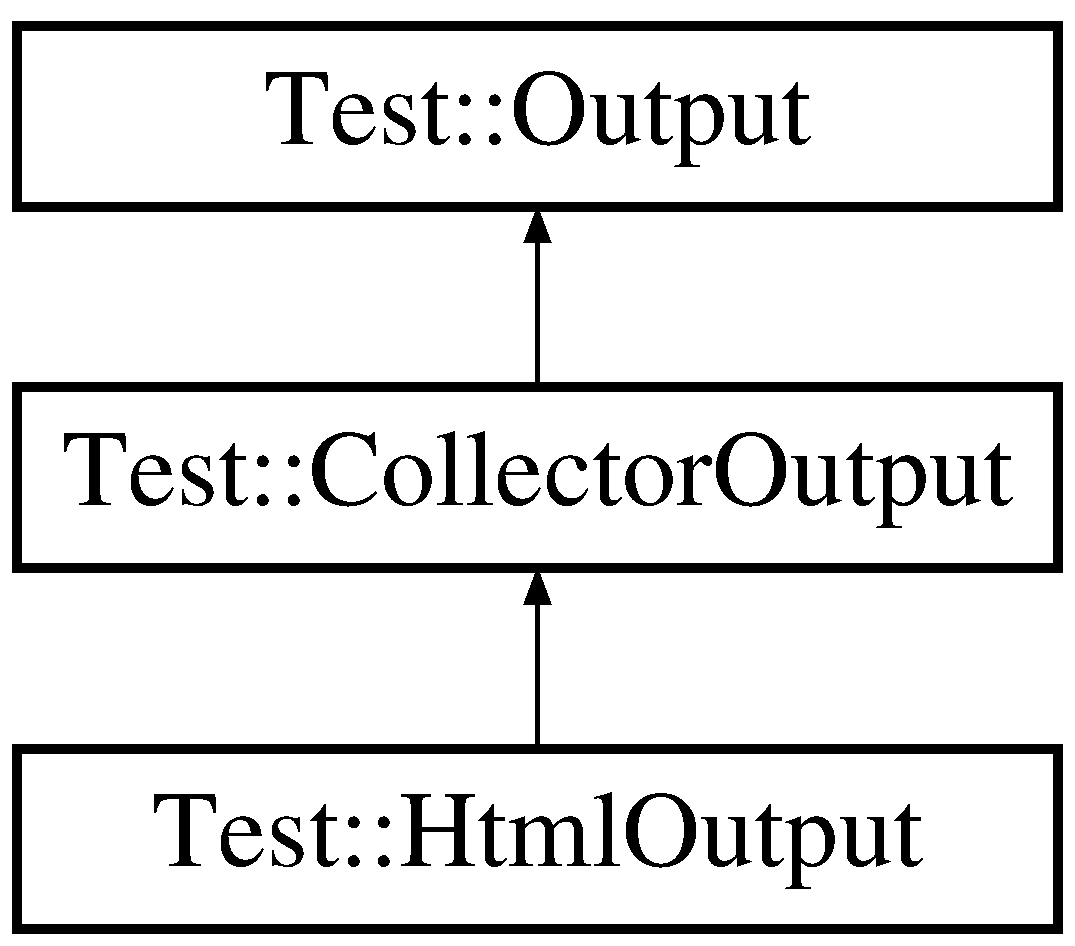
\includegraphics[height=3.000000cm]{class_test_1_1_collector_output}
\end{center}
\end{figure}
\subsection*{Classes}
\begin{DoxyCompactItemize}
\item 
struct \mbox{\hyperlink{struct_test_1_1_collector_output_1_1_suite_info}{Suite\+Info}}
\item 
struct \mbox{\hyperlink{struct_test_1_1_collector_output_1_1_test_info}{Test\+Info}}
\end{DoxyCompactItemize}
\subsection*{Public Member Functions}
\begin{DoxyCompactItemize}
\item 
virtual void \mbox{\hyperlink{class_test_1_1_collector_output_ad1a7502a31c58d93f0d88d7a679ab24d}{finished}} (int tests, const \mbox{\hyperlink{class_test_1_1_time}{Time}} \&time)
\item 
virtual void \mbox{\hyperlink{class_test_1_1_collector_output_a1d4c1eb5920fa96fb8dc8fe2eb0c336e}{suite\+\_\+start}} (int tests, const std\+::string \&name)
\item 
virtual void \mbox{\hyperlink{class_test_1_1_collector_output_a50c041adf1de3e296b50b1611e55a407}{suite\+\_\+end}} (int tests, const std\+::string \&name, const \mbox{\hyperlink{class_test_1_1_time}{Time}} \&time)
\item 
virtual void \mbox{\hyperlink{class_test_1_1_collector_output_a0ac72b71fac68305ceabb1c516760eb0}{test\+\_\+start}} (const std\+::string \&name)
\item 
virtual void \mbox{\hyperlink{class_test_1_1_collector_output_a08aa350c9a0ce221d03f6841a0b5d633}{test\+\_\+end}} (const std\+::string \&name, bool ok, const \mbox{\hyperlink{class_test_1_1_time}{Time}} \&time)
\item 
virtual void \mbox{\hyperlink{class_test_1_1_collector_output_a96b61d5e53c3dfa1b98747bb582aa4f3}{assertment}} (const \mbox{\hyperlink{class_test_1_1_source}{Source}} \&s)
\end{DoxyCompactItemize}
\subsection*{Protected Types}
\begin{DoxyCompactItemize}
\item 
typedef std\+::list$<$ \mbox{\hyperlink{class_test_1_1_source}{Source}} $>$ \mbox{\hyperlink{class_test_1_1_collector_output_a1921f35e0da596bd75da5824afe872c9}{Sources}}
\item 
typedef std\+::vector$<$ \mbox{\hyperlink{struct_test_1_1_collector_output_1_1_test_info}{Test\+Info}} $>$ \mbox{\hyperlink{class_test_1_1_collector_output_a54a7b7c9b6d181102bc8934190b06e86}{Tests}}
\item 
typedef std\+::list$<$ \mbox{\hyperlink{struct_test_1_1_collector_output_1_1_suite_info}{Suite\+Info}} $>$ \mbox{\hyperlink{class_test_1_1_collector_output_a0879ce3b51f1e3b3fe14aa5665dccd30}{Suites}}
\end{DoxyCompactItemize}
\subsection*{Protected Member Functions}
\begin{DoxyCompactItemize}
\item 
\mbox{\hyperlink{class_test_1_1_collector_output_a852bde8f194b4f81ca36f222257adc53}{Collector\+Output}} ()
\end{DoxyCompactItemize}
\subsection*{Protected Attributes}
\begin{DoxyCompactItemize}
\item 
\mbox{\hyperlink{class_test_1_1_collector_output_a0879ce3b51f1e3b3fe14aa5665dccd30}{Suites}} \mbox{\hyperlink{class_test_1_1_collector_output_a9f79c0fa5abf1d6248a85e7ae4701c5f}{\+\_\+suites}}
\item 
int \mbox{\hyperlink{class_test_1_1_collector_output_a7d8ec4ad0316b57aa96ae50a548c94d2}{\+\_\+total\+\_\+errors}}
\item 
int \mbox{\hyperlink{class_test_1_1_collector_output_ace6c1fc02a6ac7a6c15b982b96f5f68f}{\+\_\+total\+\_\+tests}}
\item 
\mbox{\hyperlink{class_test_1_1_time}{Time}} \mbox{\hyperlink{class_test_1_1_collector_output_af1e014fde4bf5b4e6c89de748630aa79}{\+\_\+total\+\_\+time}}
\end{DoxyCompactItemize}


\subsection{Detailed Description}
Collector output. 

Base class for output handlers that need to report status when all tests have executed. 

Definition at line 47 of file cpptest-\/collectoroutput.\+h.



\subsection{Member Typedef Documentation}
\mbox{\Hypertarget{class_test_1_1_collector_output_a1921f35e0da596bd75da5824afe872c9}\label{class_test_1_1_collector_output_a1921f35e0da596bd75da5824afe872c9}} 
\index{Test\+::\+Collector\+Output@{Test\+::\+Collector\+Output}!Sources@{Sources}}
\index{Sources@{Sources}!Test\+::\+Collector\+Output@{Test\+::\+Collector\+Output}}
\subsubsection{\texorpdfstring{Sources}{Sources}}
{\footnotesize\ttfamily typedef std\+::list$<$\mbox{\hyperlink{class_test_1_1_source}{Source}}$>$ \mbox{\hyperlink{class_test_1_1_collector_output_a1921f35e0da596bd75da5824afe872c9}{Test\+::\+Collector\+Output\+::\+Sources}}\hspace{0.3cm}{\ttfamily [protected]}}



Definition at line 62 of file cpptest-\/collectoroutput.\+h.

\mbox{\Hypertarget{class_test_1_1_collector_output_a0879ce3b51f1e3b3fe14aa5665dccd30}\label{class_test_1_1_collector_output_a0879ce3b51f1e3b3fe14aa5665dccd30}} 
\index{Test\+::\+Collector\+Output@{Test\+::\+Collector\+Output}!Suites@{Suites}}
\index{Suites@{Suites}!Test\+::\+Collector\+Output@{Test\+::\+Collector\+Output}}
\subsubsection{\texorpdfstring{Suites}{Suites}}
{\footnotesize\ttfamily typedef std\+::list$<$\mbox{\hyperlink{struct_test_1_1_collector_output_1_1_suite_info}{Suite\+Info}}$>$ \mbox{\hyperlink{class_test_1_1_collector_output_a0879ce3b51f1e3b3fe14aa5665dccd30}{Test\+::\+Collector\+Output\+::\+Suites}}\hspace{0.3cm}{\ttfamily [protected]}}



Definition at line 89 of file cpptest-\/collectoroutput.\+h.

\mbox{\Hypertarget{class_test_1_1_collector_output_a54a7b7c9b6d181102bc8934190b06e86}\label{class_test_1_1_collector_output_a54a7b7c9b6d181102bc8934190b06e86}} 
\index{Test\+::\+Collector\+Output@{Test\+::\+Collector\+Output}!Tests@{Tests}}
\index{Tests@{Tests}!Test\+::\+Collector\+Output@{Test\+::\+Collector\+Output}}
\subsubsection{\texorpdfstring{Tests}{Tests}}
{\footnotesize\ttfamily typedef std\+::vector$<$\mbox{\hyperlink{struct_test_1_1_collector_output_1_1_test_info}{Test\+Info}}$>$ \mbox{\hyperlink{class_test_1_1_collector_output_a54a7b7c9b6d181102bc8934190b06e86}{Test\+::\+Collector\+Output\+::\+Tests}}\hspace{0.3cm}{\ttfamily [protected]}}



Definition at line 77 of file cpptest-\/collectoroutput.\+h.



\subsection{Constructor \& Destructor Documentation}
\mbox{\Hypertarget{class_test_1_1_collector_output_a852bde8f194b4f81ca36f222257adc53}\label{class_test_1_1_collector_output_a852bde8f194b4f81ca36f222257adc53}} 
\index{Test\+::\+Collector\+Output@{Test\+::\+Collector\+Output}!Collector\+Output@{Collector\+Output}}
\index{Collector\+Output@{Collector\+Output}!Test\+::\+Collector\+Output@{Test\+::\+Collector\+Output}}
\subsubsection{\texorpdfstring{Collector\+Output()}{CollectorOutput()}}
{\footnotesize\ttfamily Test\+::\+Collector\+Output\+::\+Collector\+Output (\begin{DoxyParamCaption}{ }\end{DoxyParamCaption})\hspace{0.3cm}{\ttfamily [protected]}}



\subsection{Member Function Documentation}
\mbox{\Hypertarget{class_test_1_1_collector_output_a96b61d5e53c3dfa1b98747bb582aa4f3}\label{class_test_1_1_collector_output_a96b61d5e53c3dfa1b98747bb582aa4f3}} 
\index{Test\+::\+Collector\+Output@{Test\+::\+Collector\+Output}!assertment@{assertment}}
\index{assertment@{assertment}!Test\+::\+Collector\+Output@{Test\+::\+Collector\+Output}}
\subsubsection{\texorpdfstring{assertment()}{assertment()}}
{\footnotesize\ttfamily virtual void Test\+::\+Collector\+Output\+::assertment (\begin{DoxyParamCaption}\item[{const \mbox{\hyperlink{class_test_1_1_source}{Source}} \&}]{s }\end{DoxyParamCaption})\hspace{0.3cm}{\ttfamily [virtual]}}

Called when an assertment is issued.


\begin{DoxyParams}{Parameters}
{\em s} & Assert point information. \\
\hline
\end{DoxyParams}


Reimplemented from \mbox{\hyperlink{class_test_1_1_output_a48c31f0baa7627d81939be840c9a7f65}{Test\+::\+Output}}.

\mbox{\Hypertarget{class_test_1_1_collector_output_ad1a7502a31c58d93f0d88d7a679ab24d}\label{class_test_1_1_collector_output_ad1a7502a31c58d93f0d88d7a679ab24d}} 
\index{Test\+::\+Collector\+Output@{Test\+::\+Collector\+Output}!finished@{finished}}
\index{finished@{finished}!Test\+::\+Collector\+Output@{Test\+::\+Collector\+Output}}
\subsubsection{\texorpdfstring{finished()}{finished()}}
{\footnotesize\ttfamily virtual void Test\+::\+Collector\+Output\+::finished (\begin{DoxyParamCaption}\item[{int}]{tests,  }\item[{const \mbox{\hyperlink{class_test_1_1_time}{Time}} \&}]{time }\end{DoxyParamCaption})\hspace{0.3cm}{\ttfamily [virtual]}}

Called when testing is finished.


\begin{DoxyParams}{Parameters}
{\em tests} & Total number of tests in all suites. \\
\hline
{\em time} & Total elapsed time for all tests. \\
\hline
\end{DoxyParams}


Reimplemented from \mbox{\hyperlink{class_test_1_1_output_aeff8af8326a8c54a38199f76837f860a}{Test\+::\+Output}}.

\mbox{\Hypertarget{class_test_1_1_collector_output_a50c041adf1de3e296b50b1611e55a407}\label{class_test_1_1_collector_output_a50c041adf1de3e296b50b1611e55a407}} 
\index{Test\+::\+Collector\+Output@{Test\+::\+Collector\+Output}!suite\+\_\+end@{suite\+\_\+end}}
\index{suite\+\_\+end@{suite\+\_\+end}!Test\+::\+Collector\+Output@{Test\+::\+Collector\+Output}}
\subsubsection{\texorpdfstring{suite\+\_\+end()}{suite\_end()}}
{\footnotesize\ttfamily virtual void Test\+::\+Collector\+Output\+::suite\+\_\+end (\begin{DoxyParamCaption}\item[{int}]{tests,  }\item[{const std\+::string \&}]{name,  }\item[{const \mbox{\hyperlink{class_test_1_1_time}{Time}} \&}]{time }\end{DoxyParamCaption})\hspace{0.3cm}{\ttfamily [virtual]}}

Called when a suite is finished.


\begin{DoxyParams}{Parameters}
{\em tests} & Number of tests in this suite. \\
\hline
{\em name} & Name of the suite. \\
\hline
{\em time} & Total elapsed time for all tests in this suite. \\
\hline
\end{DoxyParams}


Reimplemented from \mbox{\hyperlink{class_test_1_1_output_a6dbf4c0adb2bd4a7364c629179f788a6}{Test\+::\+Output}}.

\mbox{\Hypertarget{class_test_1_1_collector_output_a1d4c1eb5920fa96fb8dc8fe2eb0c336e}\label{class_test_1_1_collector_output_a1d4c1eb5920fa96fb8dc8fe2eb0c336e}} 
\index{Test\+::\+Collector\+Output@{Test\+::\+Collector\+Output}!suite\+\_\+start@{suite\+\_\+start}}
\index{suite\+\_\+start@{suite\+\_\+start}!Test\+::\+Collector\+Output@{Test\+::\+Collector\+Output}}
\subsubsection{\texorpdfstring{suite\+\_\+start()}{suite\_start()}}
{\footnotesize\ttfamily virtual void Test\+::\+Collector\+Output\+::suite\+\_\+start (\begin{DoxyParamCaption}\item[{int}]{tests,  }\item[{const std\+::string \&}]{name }\end{DoxyParamCaption})\hspace{0.3cm}{\ttfamily [virtual]}}

Called when a suite is entered.


\begin{DoxyParams}{Parameters}
{\em tests} & Number of tests in this suite. \\
\hline
{\em name} & Name of the suite. \\
\hline
\end{DoxyParams}


Reimplemented from \mbox{\hyperlink{class_test_1_1_output_a7022c32c5a1577b10b93d3942746f17d}{Test\+::\+Output}}.

\mbox{\Hypertarget{class_test_1_1_collector_output_a08aa350c9a0ce221d03f6841a0b5d633}\label{class_test_1_1_collector_output_a08aa350c9a0ce221d03f6841a0b5d633}} 
\index{Test\+::\+Collector\+Output@{Test\+::\+Collector\+Output}!test\+\_\+end@{test\+\_\+end}}
\index{test\+\_\+end@{test\+\_\+end}!Test\+::\+Collector\+Output@{Test\+::\+Collector\+Output}}
\subsubsection{\texorpdfstring{test\+\_\+end()}{test\_end()}}
{\footnotesize\ttfamily virtual void Test\+::\+Collector\+Output\+::test\+\_\+end (\begin{DoxyParamCaption}\item[{const std\+::string \&}]{name,  }\item[{bool}]{ok,  }\item[{const \mbox{\hyperlink{class_test_1_1_time}{Time}} \&}]{time }\end{DoxyParamCaption})\hspace{0.3cm}{\ttfamily [virtual]}}

Called when a test if finished, regardless if an assertment was issued.


\begin{DoxyParams}{Parameters}
{\em name} & Name of the test function. \\
\hline
{\em ok} & True if the test was successful; false otherwise. \\
\hline
{\em time} & Execution time. \\
\hline
\end{DoxyParams}


Reimplemented from \mbox{\hyperlink{class_test_1_1_output_a3796943e3b56373492c957212a21454e}{Test\+::\+Output}}.

\mbox{\Hypertarget{class_test_1_1_collector_output_a0ac72b71fac68305ceabb1c516760eb0}\label{class_test_1_1_collector_output_a0ac72b71fac68305ceabb1c516760eb0}} 
\index{Test\+::\+Collector\+Output@{Test\+::\+Collector\+Output}!test\+\_\+start@{test\+\_\+start}}
\index{test\+\_\+start@{test\+\_\+start}!Test\+::\+Collector\+Output@{Test\+::\+Collector\+Output}}
\subsubsection{\texorpdfstring{test\+\_\+start()}{test\_start()}}
{\footnotesize\ttfamily virtual void Test\+::\+Collector\+Output\+::test\+\_\+start (\begin{DoxyParamCaption}\item[{const std\+::string \&}]{name }\end{DoxyParamCaption})\hspace{0.3cm}{\ttfamily [virtual]}}

Called when a tests is executed.


\begin{DoxyParams}{Parameters}
{\em name} & Name of the test function. \\
\hline
\end{DoxyParams}


Reimplemented from \mbox{\hyperlink{class_test_1_1_output_a52d43b97609febc5abbc6da9aa0abac2}{Test\+::\+Output}}.



\subsection{Member Data Documentation}
\mbox{\Hypertarget{class_test_1_1_collector_output_a9f79c0fa5abf1d6248a85e7ae4701c5f}\label{class_test_1_1_collector_output_a9f79c0fa5abf1d6248a85e7ae4701c5f}} 
\index{Test\+::\+Collector\+Output@{Test\+::\+Collector\+Output}!\+\_\+suites@{\+\_\+suites}}
\index{\+\_\+suites@{\+\_\+suites}!Test\+::\+Collector\+Output@{Test\+::\+Collector\+Output}}
\subsubsection{\texorpdfstring{\+\_\+suites}{\_suites}}
{\footnotesize\ttfamily \mbox{\hyperlink{class_test_1_1_collector_output_a0879ce3b51f1e3b3fe14aa5665dccd30}{Suites}} Test\+::\+Collector\+Output\+::\+\_\+suites\hspace{0.3cm}{\ttfamily [protected]}}



Definition at line 91 of file cpptest-\/collectoroutput.\+h.

\mbox{\Hypertarget{class_test_1_1_collector_output_a7d8ec4ad0316b57aa96ae50a548c94d2}\label{class_test_1_1_collector_output_a7d8ec4ad0316b57aa96ae50a548c94d2}} 
\index{Test\+::\+Collector\+Output@{Test\+::\+Collector\+Output}!\+\_\+total\+\_\+errors@{\+\_\+total\+\_\+errors}}
\index{\+\_\+total\+\_\+errors@{\+\_\+total\+\_\+errors}!Test\+::\+Collector\+Output@{Test\+::\+Collector\+Output}}
\subsubsection{\texorpdfstring{\+\_\+total\+\_\+errors}{\_total\_errors}}
{\footnotesize\ttfamily int Test\+::\+Collector\+Output\+::\+\_\+total\+\_\+errors\hspace{0.3cm}{\ttfamily [protected]}}



Definition at line 92 of file cpptest-\/collectoroutput.\+h.

\mbox{\Hypertarget{class_test_1_1_collector_output_ace6c1fc02a6ac7a6c15b982b96f5f68f}\label{class_test_1_1_collector_output_ace6c1fc02a6ac7a6c15b982b96f5f68f}} 
\index{Test\+::\+Collector\+Output@{Test\+::\+Collector\+Output}!\+\_\+total\+\_\+tests@{\+\_\+total\+\_\+tests}}
\index{\+\_\+total\+\_\+tests@{\+\_\+total\+\_\+tests}!Test\+::\+Collector\+Output@{Test\+::\+Collector\+Output}}
\subsubsection{\texorpdfstring{\+\_\+total\+\_\+tests}{\_total\_tests}}
{\footnotesize\ttfamily int Test\+::\+Collector\+Output\+::\+\_\+total\+\_\+tests\hspace{0.3cm}{\ttfamily [protected]}}



Definition at line 93 of file cpptest-\/collectoroutput.\+h.

\mbox{\Hypertarget{class_test_1_1_collector_output_af1e014fde4bf5b4e6c89de748630aa79}\label{class_test_1_1_collector_output_af1e014fde4bf5b4e6c89de748630aa79}} 
\index{Test\+::\+Collector\+Output@{Test\+::\+Collector\+Output}!\+\_\+total\+\_\+time@{\+\_\+total\+\_\+time}}
\index{\+\_\+total\+\_\+time@{\+\_\+total\+\_\+time}!Test\+::\+Collector\+Output@{Test\+::\+Collector\+Output}}
\subsubsection{\texorpdfstring{\+\_\+total\+\_\+time}{\_total\_time}}
{\footnotesize\ttfamily \mbox{\hyperlink{class_test_1_1_time}{Time}} Test\+::\+Collector\+Output\+::\+\_\+total\+\_\+time\hspace{0.3cm}{\ttfamily [protected]}}



Definition at line 94 of file cpptest-\/collectoroutput.\+h.



The documentation for this class was generated from the following file\+:\begin{DoxyCompactItemize}
\item 
\mbox{\hyperlink{cpptest-collectoroutput_8h}{cpptest-\/collectoroutput.\+h}}\end{DoxyCompactItemize}

\hypertarget{class_test_1_1_compiler_output}{}\section{Test\+:\+:Compiler\+Output Class Reference}
\label{class_test_1_1_compiler_output}\index{Test\+::\+Compiler\+Output@{Test\+::\+Compiler\+Output}}


Compiler-\/like output handler.  




{\ttfamily \#include $<$cpptest-\/compileroutput.\+h$>$}

Inheritance diagram for Test\+:\+:Compiler\+Output\+:\begin{figure}[H]
\begin{center}
\leavevmode
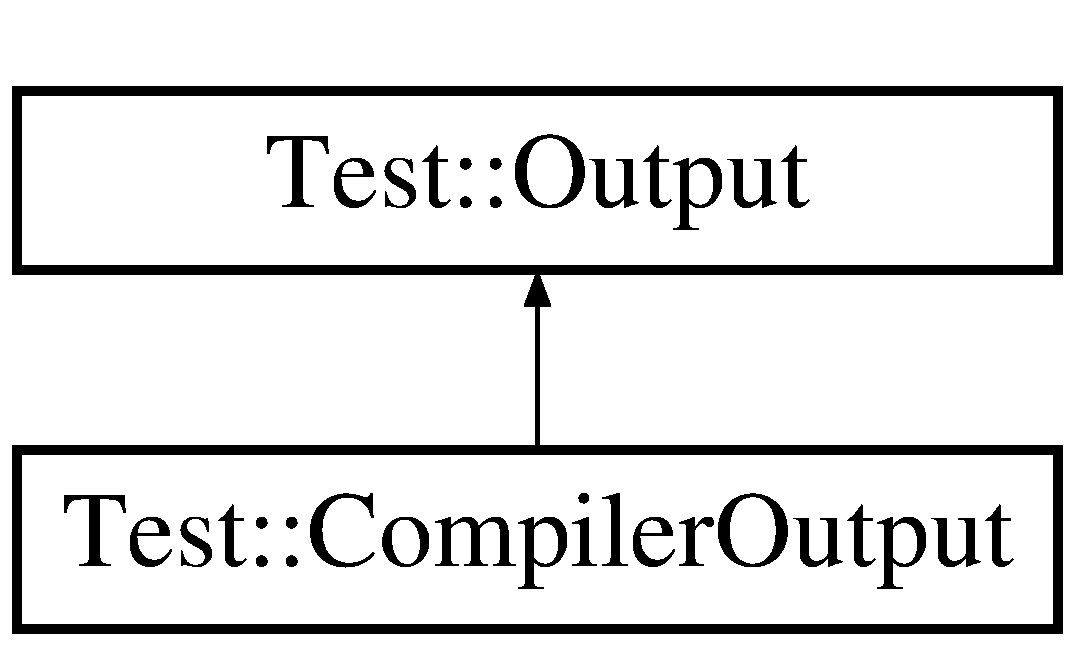
\includegraphics[height=2.000000cm]{class_test_1_1_compiler_output}
\end{center}
\end{figure}
\subsection*{Classes}
\begin{DoxyCompactItemize}
\item 
class \mbox{\hyperlink{class_test_1_1_compiler_output_1_1_invalid_format}{Invalid\+Format}}
\begin{DoxyCompactList}\small\item\em Compiler output exception. \end{DoxyCompactList}\end{DoxyCompactItemize}
\subsection*{Public Types}
\begin{DoxyCompactItemize}
\item 
enum \mbox{\hyperlink{class_test_1_1_compiler_output_ab34cf506804cefbc67545a256af196ff}{Format}} \{ \mbox{\hyperlink{class_test_1_1_compiler_output_ab34cf506804cefbc67545a256af196ffa1a83926858dfb1bab06bc0a313a49dac}{Generic}}, 
\mbox{\hyperlink{class_test_1_1_compiler_output_ab34cf506804cefbc67545a256af196ffa9ad6dc16df2c992e8b77a3f6ee2247d8}{B\+CC}}, 
\mbox{\hyperlink{class_test_1_1_compiler_output_ab34cf506804cefbc67545a256af196ffa7d077829f643d60a87a022d39989dd3b}{G\+CC}}, 
\mbox{\hyperlink{class_test_1_1_compiler_output_ab34cf506804cefbc67545a256af196ffae4f7af0eaa05253ea35484384deeb86b}{M\+S\+VC}}
 \}
\end{DoxyCompactItemize}
\subsection*{Public Member Functions}
\begin{DoxyCompactItemize}
\item 
\mbox{\hyperlink{class_test_1_1_compiler_output_a816ae9a0ff2fb6cbb95c7cd815a6e621}{Compiler\+Output}} (\mbox{\hyperlink{class_test_1_1_compiler_output_ab34cf506804cefbc67545a256af196ff}{Format}} format=\mbox{\hyperlink{class_test_1_1_compiler_output_ab34cf506804cefbc67545a256af196ffa1a83926858dfb1bab06bc0a313a49dac}{Generic}}, std\+::ostream \&stream=std\+::cout)
\item 
\mbox{\hyperlink{class_test_1_1_compiler_output_a49f7092d23ce60e3b83fa30fb5ab9ab7}{Compiler\+Output}} (const std\+::string \&format, std\+::ostream \&stream=std\+::cout)
\item 
virtual void \mbox{\hyperlink{class_test_1_1_compiler_output_a1c36e3fd12afe3556e887349b0b86b50}{assertment}} (const \mbox{\hyperlink{class_test_1_1_source}{Source}} \&s)
\end{DoxyCompactItemize}
\subsection*{Additional Inherited Members}


\subsection{Detailed Description}
Compiler-\/like output handler. 

Test suite output handler that only outputs failures in compiler warning/error format. This way, you can use your I\+DE to browse between failures.

The output format is configurable to be able to emulate different compiler outputs. The following modifiers exist\+:
\begin{DoxyItemize}
\item {\itshape file} Outputs the file containing the test function.
\item {\itshape line} Line number for the the test function.
\item {\itshape text} Expression (or message) that caused the assertment. Note that each modifier can only be specified once. 
\end{DoxyItemize}

Definition at line 52 of file cpptest-\/compileroutput.\+h.



\subsection{Member Enumeration Documentation}
\mbox{\Hypertarget{class_test_1_1_compiler_output_ab34cf506804cefbc67545a256af196ff}\label{class_test_1_1_compiler_output_ab34cf506804cefbc67545a256af196ff}} 
\index{Test\+::\+Compiler\+Output@{Test\+::\+Compiler\+Output}!Format@{Format}}
\index{Format@{Format}!Test\+::\+Compiler\+Output@{Test\+::\+Compiler\+Output}}
\subsubsection{\texorpdfstring{Format}{Format}}
{\footnotesize\ttfamily enum \mbox{\hyperlink{class_test_1_1_compiler_output_ab34cf506804cefbc67545a256af196ff}{Test\+::\+Compiler\+Output\+::\+Format}}}

Pre-\/defined compiler output formats. \begin{DoxyEnumFields}{Enumerator}
\raisebox{\heightof{T}}[0pt][0pt]{\index{Generic@{Generic}!Test\+::\+Compiler\+Output@{Test\+::\+Compiler\+Output}}\index{Test\+::\+Compiler\+Output@{Test\+::\+Compiler\+Output}!Generic@{Generic}}}\mbox{\Hypertarget{class_test_1_1_compiler_output_ab34cf506804cefbc67545a256af196ffa1a83926858dfb1bab06bc0a313a49dac}\label{class_test_1_1_compiler_output_ab34cf506804cefbc67545a256af196ffa1a83926858dfb1bab06bc0a313a49dac}} 
Generic&Generic compiler format, which equals\+: {\ttfamily \%file\+:\%line\+: \%text} \\
\hline

\raisebox{\heightof{T}}[0pt][0pt]{\index{B\+CC@{B\+CC}!Test\+::\+Compiler\+Output@{Test\+::\+Compiler\+Output}}\index{Test\+::\+Compiler\+Output@{Test\+::\+Compiler\+Output}!B\+CC@{B\+CC}}}\mbox{\Hypertarget{class_test_1_1_compiler_output_ab34cf506804cefbc67545a256af196ffa9ad6dc16df2c992e8b77a3f6ee2247d8}\label{class_test_1_1_compiler_output_ab34cf506804cefbc67545a256af196ffa9ad6dc16df2c992e8b77a3f6ee2247d8}} 
B\+CC&\href{http://www.borland.com/products/downloads/download_cbuilder.html}{\tt Borland C++ Compiler} (B\+CC) format, which equals\+: {\ttfamily Error cpptest \%file \%line\+: \%text}. \\
\hline

\raisebox{\heightof{T}}[0pt][0pt]{\index{G\+CC@{G\+CC}!Test\+::\+Compiler\+Output@{Test\+::\+Compiler\+Output}}\index{Test\+::\+Compiler\+Output@{Test\+::\+Compiler\+Output}!G\+CC@{G\+CC}}}\mbox{\Hypertarget{class_test_1_1_compiler_output_ab34cf506804cefbc67545a256af196ffa7d077829f643d60a87a022d39989dd3b}\label{class_test_1_1_compiler_output_ab34cf506804cefbc67545a256af196ffa7d077829f643d60a87a022d39989dd3b}} 
G\+CC&\href{http://gcc.gnu.org}{\tt G\+NU Compiler Collection} (G\+CC) format, which equals\+: {\ttfamily \%file\+:\%line\+: \%text} \\
\hline

\raisebox{\heightof{T}}[0pt][0pt]{\index{M\+S\+VC@{M\+S\+VC}!Test\+::\+Compiler\+Output@{Test\+::\+Compiler\+Output}}\index{Test\+::\+Compiler\+Output@{Test\+::\+Compiler\+Output}!M\+S\+VC@{M\+S\+VC}}}\mbox{\Hypertarget{class_test_1_1_compiler_output_ab34cf506804cefbc67545a256af196ffae4f7af0eaa05253ea35484384deeb86b}\label{class_test_1_1_compiler_output_ab34cf506804cefbc67545a256af196ffae4f7af0eaa05253ea35484384deeb86b}} 
M\+S\+VC&\href{http://www.microsoft.com}{\tt Microsoft Visual C++} (M\+S\+VC) format, which equals\+: {\ttfamily \%file(\%line) \+: \%text} \\
\hline

\end{DoxyEnumFields}


Definition at line 70 of file cpptest-\/compileroutput.\+h.



\subsection{Constructor \& Destructor Documentation}
\mbox{\Hypertarget{class_test_1_1_compiler_output_a816ae9a0ff2fb6cbb95c7cd815a6e621}\label{class_test_1_1_compiler_output_a816ae9a0ff2fb6cbb95c7cd815a6e621}} 
\index{Test\+::\+Compiler\+Output@{Test\+::\+Compiler\+Output}!Compiler\+Output@{Compiler\+Output}}
\index{Compiler\+Output@{Compiler\+Output}!Test\+::\+Compiler\+Output@{Test\+::\+Compiler\+Output}}
\subsubsection{\texorpdfstring{Compiler\+Output()}{CompilerOutput()}\hspace{0.1cm}{\footnotesize\ttfamily [1/2]}}
{\footnotesize\ttfamily Test\+::\+Compiler\+Output\+::\+Compiler\+Output (\begin{DoxyParamCaption}\item[{\mbox{\hyperlink{class_test_1_1_compiler_output_ab34cf506804cefbc67545a256af196ff}{Format}}}]{format = {\ttfamily \mbox{\hyperlink{class_test_1_1_compiler_output_ab34cf506804cefbc67545a256af196ffa1a83926858dfb1bab06bc0a313a49dac}{Generic}}},  }\item[{std\+::ostream \&}]{stream = {\ttfamily std\+:\+:cout} }\end{DoxyParamCaption})\hspace{0.3cm}{\ttfamily [explicit]}}

\mbox{\Hypertarget{class_test_1_1_compiler_output_a49f7092d23ce60e3b83fa30fb5ab9ab7}\label{class_test_1_1_compiler_output_a49f7092d23ce60e3b83fa30fb5ab9ab7}} 
\index{Test\+::\+Compiler\+Output@{Test\+::\+Compiler\+Output}!Compiler\+Output@{Compiler\+Output}}
\index{Compiler\+Output@{Compiler\+Output}!Test\+::\+Compiler\+Output@{Test\+::\+Compiler\+Output}}
\subsubsection{\texorpdfstring{Compiler\+Output()}{CompilerOutput()}\hspace{0.1cm}{\footnotesize\ttfamily [2/2]}}
{\footnotesize\ttfamily Test\+::\+Compiler\+Output\+::\+Compiler\+Output (\begin{DoxyParamCaption}\item[{const std\+::string \&}]{format,  }\item[{std\+::ostream \&}]{stream = {\ttfamily std\+:\+:cout} }\end{DoxyParamCaption})\hspace{0.3cm}{\ttfamily [explicit]}}



\subsection{Member Function Documentation}
\mbox{\Hypertarget{class_test_1_1_compiler_output_a1c36e3fd12afe3556e887349b0b86b50}\label{class_test_1_1_compiler_output_a1c36e3fd12afe3556e887349b0b86b50}} 
\index{Test\+::\+Compiler\+Output@{Test\+::\+Compiler\+Output}!assertment@{assertment}}
\index{assertment@{assertment}!Test\+::\+Compiler\+Output@{Test\+::\+Compiler\+Output}}
\subsubsection{\texorpdfstring{assertment()}{assertment()}}
{\footnotesize\ttfamily virtual void Test\+::\+Compiler\+Output\+::assertment (\begin{DoxyParamCaption}\item[{const \mbox{\hyperlink{class_test_1_1_source}{Source}} \&}]{s }\end{DoxyParamCaption})\hspace{0.3cm}{\ttfamily [virtual]}}

Called when an assertment is issued.


\begin{DoxyParams}{Parameters}
{\em s} & Assert point information. \\
\hline
\end{DoxyParams}


Reimplemented from \mbox{\hyperlink{class_test_1_1_output_a48c31f0baa7627d81939be840c9a7f65}{Test\+::\+Output}}.



The documentation for this class was generated from the following file\+:\begin{DoxyCompactItemize}
\item 
\mbox{\hyperlink{cpptest-compileroutput_8h}{cpptest-\/compileroutput.\+h}}\end{DoxyCompactItemize}

\hypertarget{classdb_test}{}\section{db\+Test Class Reference}
\label{classdb_test}\index{db\+Test@{db\+Test}}
Inheritance diagram for db\+Test\+:\begin{figure}[H]
\begin{center}
\leavevmode
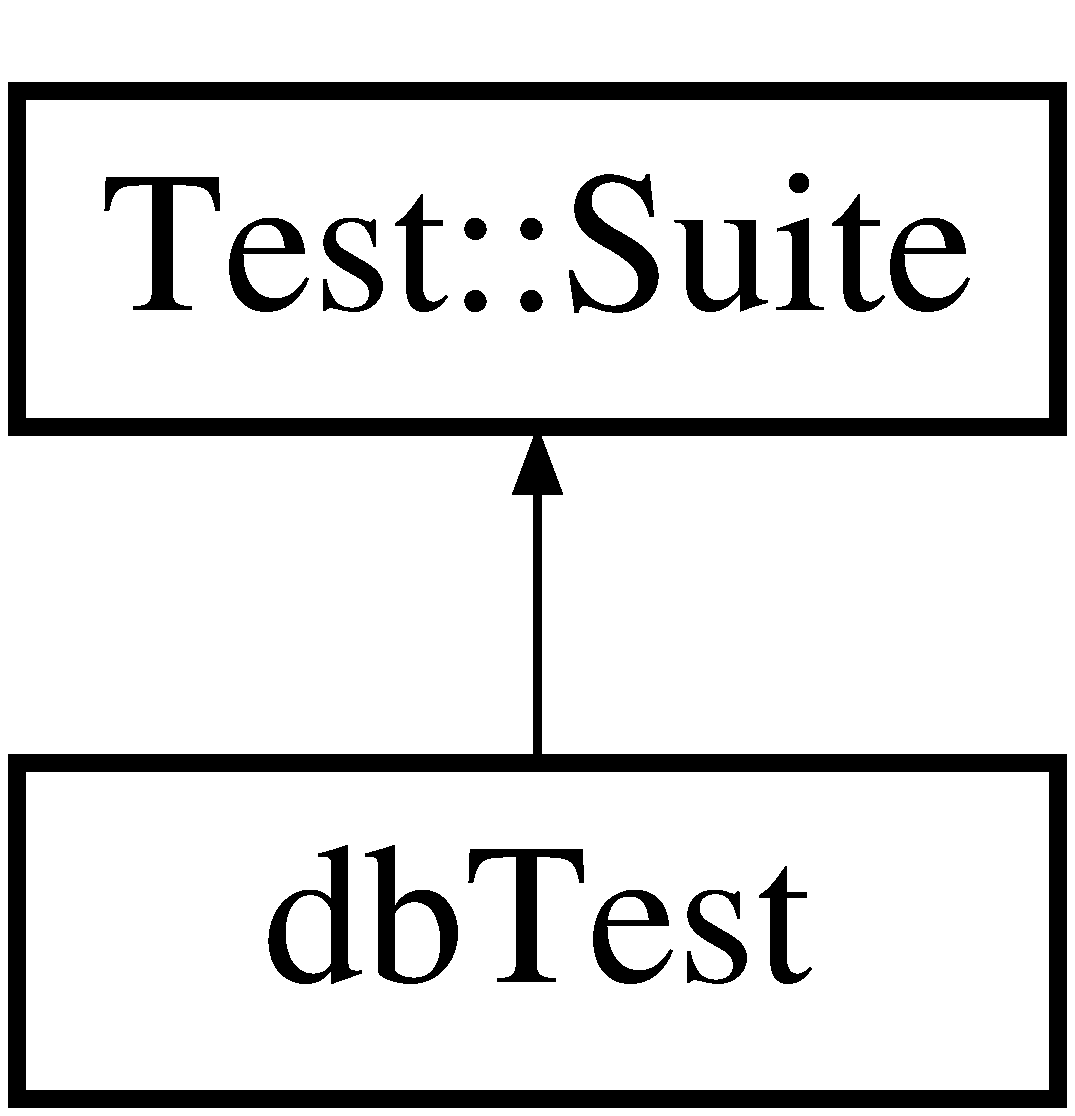
\includegraphics[height=2.000000cm]{classdb_test}
\end{center}
\end{figure}
\subsection*{Public Member Functions}
\begin{DoxyCompactItemize}
\item 
\mbox{\hyperlink{classdb_test_aef2697ca1fc1a9368f220d8b5e62402d}{db\+Test}} ()
\end{DoxyCompactItemize}
\subsection*{Protected Member Functions}
\begin{DoxyCompactItemize}
\item 
virtual void \mbox{\hyperlink{classdb_test_aeefb6e8d64ee6e03da89cb5573d60b31}{setup}} ()
\item 
virtual void \mbox{\hyperlink{classdb_test_a1fa8de6f80f7578356b0f8feb8dcdd8f}{tear\+\_\+down}} ()
\end{DoxyCompactItemize}
\subsection*{Protected Attributes}
\begin{DoxyCompactItemize}
\item 
\mbox{\hyperlink{class_record_processor}{Record\+Processor}} \mbox{\hyperlink{classdb_test_a9edd9165f54a1ad52545ebff71686735}{processor}}
\end{DoxyCompactItemize}
\subsection*{Additional Inherited Members}


\subsection{Detailed Description}


Definition at line 11 of file Console\+Application1.\+cpp.



\subsection{Constructor \& Destructor Documentation}
\mbox{\Hypertarget{classdb_test_aef2697ca1fc1a9368f220d8b5e62402d}\label{classdb_test_aef2697ca1fc1a9368f220d8b5e62402d}} 
\index{db\+Test@{db\+Test}!db\+Test@{db\+Test}}
\index{db\+Test@{db\+Test}!db\+Test@{db\+Test}}
\subsubsection{\texorpdfstring{db\+Test()}{dbTest()}}
{\footnotesize\ttfamily db\+Test\+::db\+Test (\begin{DoxyParamCaption}{ }\end{DoxyParamCaption})\hspace{0.3cm}{\ttfamily [inline]}}



Definition at line 112 of file Console\+Application1.\+cpp.



\subsection{Member Function Documentation}
\mbox{\Hypertarget{classdb_test_aeefb6e8d64ee6e03da89cb5573d60b31}\label{classdb_test_aeefb6e8d64ee6e03da89cb5573d60b31}} 
\index{db\+Test@{db\+Test}!setup@{setup}}
\index{setup@{setup}!db\+Test@{db\+Test}}
\subsubsection{\texorpdfstring{setup()}{setup()}}
{\footnotesize\ttfamily virtual void db\+Test\+::setup (\begin{DoxyParamCaption}{ }\end{DoxyParamCaption})\hspace{0.3cm}{\ttfamily [inline]}, {\ttfamily [protected]}, {\ttfamily [virtual]}}



Reimplemented from \mbox{\hyperlink{class_test_1_1_suite_aa022f93f2bc7c0ca4f8bf0bb94758226}{Test\+::\+Suite}}.



Definition at line 124 of file Console\+Application1.\+cpp.

\mbox{\Hypertarget{classdb_test_a1fa8de6f80f7578356b0f8feb8dcdd8f}\label{classdb_test_a1fa8de6f80f7578356b0f8feb8dcdd8f}} 
\index{db\+Test@{db\+Test}!tear\+\_\+down@{tear\+\_\+down}}
\index{tear\+\_\+down@{tear\+\_\+down}!db\+Test@{db\+Test}}
\subsubsection{\texorpdfstring{tear\+\_\+down()}{tear\_down()}}
{\footnotesize\ttfamily virtual void db\+Test\+::tear\+\_\+down (\begin{DoxyParamCaption}{ }\end{DoxyParamCaption})\hspace{0.3cm}{\ttfamily [inline]}, {\ttfamily [protected]}, {\ttfamily [virtual]}}



Reimplemented from \mbox{\hyperlink{class_test_1_1_suite_a2f2f180307180f8fdb0ca718a12047d0}{Test\+::\+Suite}}.



Definition at line 139 of file Console\+Application1.\+cpp.



\subsection{Member Data Documentation}
\mbox{\Hypertarget{classdb_test_a9edd9165f54a1ad52545ebff71686735}\label{classdb_test_a9edd9165f54a1ad52545ebff71686735}} 
\index{db\+Test@{db\+Test}!processor@{processor}}
\index{processor@{processor}!db\+Test@{db\+Test}}
\subsubsection{\texorpdfstring{processor}{processor}}
{\footnotesize\ttfamily \mbox{\hyperlink{class_record_processor}{Record\+Processor}} db\+Test\+::processor\hspace{0.3cm}{\ttfamily [protected]}}



Definition at line 122 of file Console\+Application1.\+cpp.



The documentation for this class was generated from the following file\+:\begin{DoxyCompactItemize}
\item 
\mbox{\hyperlink{_console_application1_8cpp}{Console\+Application1.\+cpp}}\end{DoxyCompactItemize}

\hypertarget{structfts5__api}{}\section{fts5\+\_\+api Struct Reference}
\label{structfts5__api}\index{fts5\+\_\+api@{fts5\+\_\+api}}


{\ttfamily \#include $<$sqlite3.\+h$>$}

\subsection*{Public Attributes}
\begin{DoxyCompactItemize}
\item 
int \mbox{\hyperlink{structfts5__api_a3c338289abb33e1805da870172956a7c}{i\+Version}}
\item 
int($\ast$ \mbox{\hyperlink{structfts5__api_a7fe3663f85eab512d5c461e1674da129}{x\+Create\+Tokenizer}} )(\mbox{\hyperlink{structfts5__api}{fts5\+\_\+api}} $\ast$p\+Api, const char $\ast$z\+Name, void $\ast$p\+Context, \mbox{\hyperlink{structfts5__tokenizer}{fts5\+\_\+tokenizer}} $\ast$p\+Tokenizer, void($\ast$x\+Destroy)(void $\ast$))
\item 
int($\ast$ \mbox{\hyperlink{structfts5__api_a20a23794695fa61e2892ad1243b16b67}{x\+Find\+Tokenizer}} )(\mbox{\hyperlink{structfts5__api}{fts5\+\_\+api}} $\ast$p\+Api, const char $\ast$z\+Name, void $\ast$$\ast$pp\+Context, \mbox{\hyperlink{structfts5__tokenizer}{fts5\+\_\+tokenizer}} $\ast$p\+Tokenizer)
\item 
int($\ast$ \mbox{\hyperlink{structfts5__api_acf1a0612be3b91b908f38ecbc6735d17}{x\+Create\+Function}} )(\mbox{\hyperlink{structfts5__api}{fts5\+\_\+api}} $\ast$p\+Api, const char $\ast$z\+Name, void $\ast$p\+Context, \mbox{\hyperlink{sqlite3_8h_a8a1df7b5a066b194f490be5936e85c17}{fts5\+\_\+extension\+\_\+function}} x\+Function, void($\ast$x\+Destroy)(void $\ast$))
\end{DoxyCompactItemize}


\subsection{Detailed Description}


Definition at line 10687 of file sqlite3.\+h.



\subsection{Member Data Documentation}
\mbox{\Hypertarget{structfts5__api_a3c338289abb33e1805da870172956a7c}\label{structfts5__api_a3c338289abb33e1805da870172956a7c}} 
\index{fts5\+\_\+api@{fts5\+\_\+api}!i\+Version@{i\+Version}}
\index{i\+Version@{i\+Version}!fts5\+\_\+api@{fts5\+\_\+api}}
\subsubsection{\texorpdfstring{i\+Version}{iVersion}}
{\footnotesize\ttfamily int fts5\+\_\+api\+::i\+Version}



Definition at line 10688 of file sqlite3.\+h.

\mbox{\Hypertarget{structfts5__api_acf1a0612be3b91b908f38ecbc6735d17}\label{structfts5__api_acf1a0612be3b91b908f38ecbc6735d17}} 
\index{fts5\+\_\+api@{fts5\+\_\+api}!x\+Create\+Function@{x\+Create\+Function}}
\index{x\+Create\+Function@{x\+Create\+Function}!fts5\+\_\+api@{fts5\+\_\+api}}
\subsubsection{\texorpdfstring{x\+Create\+Function}{xCreateFunction}}
{\footnotesize\ttfamily int($\ast$ fts5\+\_\+api\+::x\+Create\+Function) (\mbox{\hyperlink{structfts5__api}{fts5\+\_\+api}} $\ast$p\+Api, const char $\ast$z\+Name, void $\ast$p\+Context, \mbox{\hyperlink{sqlite3_8h_a8a1df7b5a066b194f490be5936e85c17}{fts5\+\_\+extension\+\_\+function}} x\+Function, void($\ast$x\+Destroy)(void $\ast$))}



Definition at line 10708 of file sqlite3.\+h.

\mbox{\Hypertarget{structfts5__api_a7fe3663f85eab512d5c461e1674da129}\label{structfts5__api_a7fe3663f85eab512d5c461e1674da129}} 
\index{fts5\+\_\+api@{fts5\+\_\+api}!x\+Create\+Tokenizer@{x\+Create\+Tokenizer}}
\index{x\+Create\+Tokenizer@{x\+Create\+Tokenizer}!fts5\+\_\+api@{fts5\+\_\+api}}
\subsubsection{\texorpdfstring{x\+Create\+Tokenizer}{xCreateTokenizer}}
{\footnotesize\ttfamily int($\ast$ fts5\+\_\+api\+::x\+Create\+Tokenizer) (\mbox{\hyperlink{structfts5__api}{fts5\+\_\+api}} $\ast$p\+Api, const char $\ast$z\+Name, void $\ast$p\+Context, \mbox{\hyperlink{structfts5__tokenizer}{fts5\+\_\+tokenizer}} $\ast$p\+Tokenizer, void($\ast$x\+Destroy)(void $\ast$))}



Definition at line 10691 of file sqlite3.\+h.

\mbox{\Hypertarget{structfts5__api_a20a23794695fa61e2892ad1243b16b67}\label{structfts5__api_a20a23794695fa61e2892ad1243b16b67}} 
\index{fts5\+\_\+api@{fts5\+\_\+api}!x\+Find\+Tokenizer@{x\+Find\+Tokenizer}}
\index{x\+Find\+Tokenizer@{x\+Find\+Tokenizer}!fts5\+\_\+api@{fts5\+\_\+api}}
\subsubsection{\texorpdfstring{x\+Find\+Tokenizer}{xFindTokenizer}}
{\footnotesize\ttfamily int($\ast$ fts5\+\_\+api\+::x\+Find\+Tokenizer) (\mbox{\hyperlink{structfts5__api}{fts5\+\_\+api}} $\ast$p\+Api, const char $\ast$z\+Name, void $\ast$$\ast$pp\+Context, \mbox{\hyperlink{structfts5__tokenizer}{fts5\+\_\+tokenizer}} $\ast$p\+Tokenizer)}



Definition at line 10700 of file sqlite3.\+h.



The documentation for this struct was generated from the following file\+:\begin{DoxyCompactItemize}
\item 
\mbox{\hyperlink{sqlite3_8h}{sqlite3.\+h}}\end{DoxyCompactItemize}

\hypertarget{structfts5__tokenizer}{}\section{fts5\+\_\+tokenizer Struct Reference}
\label{structfts5__tokenizer}\index{fts5\+\_\+tokenizer@{fts5\+\_\+tokenizer}}


{\ttfamily \#include $<$sqlite3.\+h$>$}

\subsection*{Public Attributes}
\begin{DoxyCompactItemize}
\item 
int($\ast$ \mbox{\hyperlink{structfts5__tokenizer_a61846ad000b2d38a1264c342c8201d5c}{x\+Create}} )(void $\ast$, const char $\ast$$\ast$az\+Arg, int n\+Arg, \mbox{\hyperlink{sqlite3_8h_ac015f88c5332d612a3125fc0014e468c}{Fts5\+Tokenizer}} $\ast$$\ast$pp\+Out)
\item 
void($\ast$ \mbox{\hyperlink{structfts5__tokenizer_aaaa88b9f3e50f0b1120a05fb1bbb251f}{x\+Delete}} )(\mbox{\hyperlink{sqlite3_8h_ac015f88c5332d612a3125fc0014e468c}{Fts5\+Tokenizer}} $\ast$)
\item 
int($\ast$ \mbox{\hyperlink{structfts5__tokenizer_ae65ca5a9b1e6d5c1ef09731fccefa577}{x\+Tokenize}} )(\mbox{\hyperlink{sqlite3_8h_ac015f88c5332d612a3125fc0014e468c}{Fts5\+Tokenizer}} $\ast$, void $\ast$p\+Ctx, int flags, const char $\ast$p\+Text, int n\+Text, int($\ast$x\+Token)(void $\ast$p\+Ctx, int tflags, const char $\ast$p\+Token, int n\+Token, int i\+Start, int i\+End))
\end{DoxyCompactItemize}


\subsection{Detailed Description}


Definition at line 10651 of file sqlite3.\+h.



\subsection{Member Data Documentation}
\mbox{\Hypertarget{structfts5__tokenizer_a61846ad000b2d38a1264c342c8201d5c}\label{structfts5__tokenizer_a61846ad000b2d38a1264c342c8201d5c}} 
\index{fts5\+\_\+tokenizer@{fts5\+\_\+tokenizer}!x\+Create@{x\+Create}}
\index{x\+Create@{x\+Create}!fts5\+\_\+tokenizer@{fts5\+\_\+tokenizer}}
\subsubsection{\texorpdfstring{x\+Create}{xCreate}}
{\footnotesize\ttfamily int($\ast$ fts5\+\_\+tokenizer\+::x\+Create) (void $\ast$, const char $\ast$$\ast$az\+Arg, int n\+Arg, \mbox{\hyperlink{sqlite3_8h_ac015f88c5332d612a3125fc0014e468c}{Fts5\+Tokenizer}} $\ast$$\ast$pp\+Out)}



Definition at line 10652 of file sqlite3.\+h.

\mbox{\Hypertarget{structfts5__tokenizer_aaaa88b9f3e50f0b1120a05fb1bbb251f}\label{structfts5__tokenizer_aaaa88b9f3e50f0b1120a05fb1bbb251f}} 
\index{fts5\+\_\+tokenizer@{fts5\+\_\+tokenizer}!x\+Delete@{x\+Delete}}
\index{x\+Delete@{x\+Delete}!fts5\+\_\+tokenizer@{fts5\+\_\+tokenizer}}
\subsubsection{\texorpdfstring{x\+Delete}{xDelete}}
{\footnotesize\ttfamily void($\ast$ fts5\+\_\+tokenizer\+::x\+Delete) (\mbox{\hyperlink{sqlite3_8h_ac015f88c5332d612a3125fc0014e468c}{Fts5\+Tokenizer}} $\ast$)}



Definition at line 10653 of file sqlite3.\+h.

\mbox{\Hypertarget{structfts5__tokenizer_ae65ca5a9b1e6d5c1ef09731fccefa577}\label{structfts5__tokenizer_ae65ca5a9b1e6d5c1ef09731fccefa577}} 
\index{fts5\+\_\+tokenizer@{fts5\+\_\+tokenizer}!x\+Tokenize@{x\+Tokenize}}
\index{x\+Tokenize@{x\+Tokenize}!fts5\+\_\+tokenizer@{fts5\+\_\+tokenizer}}
\subsubsection{\texorpdfstring{x\+Tokenize}{xTokenize}}
{\footnotesize\ttfamily int($\ast$ fts5\+\_\+tokenizer\+::x\+Tokenize) (\mbox{\hyperlink{sqlite3_8h_ac015f88c5332d612a3125fc0014e468c}{Fts5\+Tokenizer}} $\ast$, void $\ast$p\+Ctx, int flags, const char $\ast$p\+Text, int n\+Text, int($\ast$x\+Token)( void $\ast$p\+Ctx, int tflags, const char $\ast$p\+Token, int n\+Token, int i\+Start, int i\+End))}



Definition at line 10654 of file sqlite3.\+h.



The documentation for this struct was generated from the following file\+:\begin{DoxyCompactItemize}
\item 
\mbox{\hyperlink{sqlite3_8h}{sqlite3.\+h}}\end{DoxyCompactItemize}

\hypertarget{struct_fts5_extension_api}{}\section{Fts5\+Extension\+Api Struct Reference}
\label{struct_fts5_extension_api}\index{Fts5\+Extension\+Api@{Fts5\+Extension\+Api}}


{\ttfamily \#include $<$sqlite3.\+h$>$}

\subsection*{Public Attributes}
\begin{DoxyCompactItemize}
\item 
int \mbox{\hyperlink{struct_fts5_extension_api_af9c8f09c2e6f1373e6bce57ec9861682}{i\+Version}}
\item 
void $\ast$($\ast$ \mbox{\hyperlink{struct_fts5_extension_api_a8e651288d8e0cf25f20f2b838f47ac34}{x\+User\+Data}} )(\mbox{\hyperlink{sqlite3_8h_a97821b95ebebd43db901977ffd5b26bc}{Fts5\+Context}} $\ast$)
\item 
int($\ast$ \mbox{\hyperlink{struct_fts5_extension_api_a427409c50da4e179c8f2d36b22a4ba21}{x\+Column\+Count}} )(\mbox{\hyperlink{sqlite3_8h_a97821b95ebebd43db901977ffd5b26bc}{Fts5\+Context}} $\ast$)
\item 
int($\ast$ \mbox{\hyperlink{struct_fts5_extension_api_ae1eb7ad1d3c131a09376134ecc099568}{x\+Row\+Count}} )(\mbox{\hyperlink{sqlite3_8h_a97821b95ebebd43db901977ffd5b26bc}{Fts5\+Context}} $\ast$, \mbox{\hyperlink{sqlite3_8h_a0a4d3e6c1ad46f90e746b920ab6ca0d2}{sqlite3\+\_\+int64}} $\ast$pn\+Row)
\item 
int($\ast$ \mbox{\hyperlink{struct_fts5_extension_api_a096e79406ae03df9796a2082d0ac8269}{x\+Column\+Total\+Size}} )(\mbox{\hyperlink{sqlite3_8h_a97821b95ebebd43db901977ffd5b26bc}{Fts5\+Context}} $\ast$, int i\+Col, \mbox{\hyperlink{sqlite3_8h_a0a4d3e6c1ad46f90e746b920ab6ca0d2}{sqlite3\+\_\+int64}} $\ast$pn\+Token)
\item 
int($\ast$ \mbox{\hyperlink{struct_fts5_extension_api_a670af0d7715f69834376f8df187dcf30}{x\+Tokenize}} )(\mbox{\hyperlink{sqlite3_8h_a97821b95ebebd43db901977ffd5b26bc}{Fts5\+Context}} $\ast$, const char $\ast$p\+Text, int n\+Text, void $\ast$p\+Ctx, int($\ast$x\+Token)(void $\ast$, int, const char $\ast$, int, int, int))
\item 
int($\ast$ \mbox{\hyperlink{struct_fts5_extension_api_a3ba0207080a9ca498625eefcc120bf1e}{x\+Phrase\+Count}} )(\mbox{\hyperlink{sqlite3_8h_a97821b95ebebd43db901977ffd5b26bc}{Fts5\+Context}} $\ast$)
\item 
int($\ast$ \mbox{\hyperlink{struct_fts5_extension_api_aeda6faa66f47f9116c9ceba882aaedd2}{x\+Phrase\+Size}} )(\mbox{\hyperlink{sqlite3_8h_a97821b95ebebd43db901977ffd5b26bc}{Fts5\+Context}} $\ast$, int i\+Phrase)
\item 
int($\ast$ \mbox{\hyperlink{struct_fts5_extension_api_af57aff7a8aa8402bb37a77892c4daf45}{x\+Inst\+Count}} )(\mbox{\hyperlink{sqlite3_8h_a97821b95ebebd43db901977ffd5b26bc}{Fts5\+Context}} $\ast$, int $\ast$pn\+Inst)
\item 
int($\ast$ \mbox{\hyperlink{struct_fts5_extension_api_a85e17f20db782b20b503f1d803a47a9e}{x\+Inst}} )(\mbox{\hyperlink{sqlite3_8h_a97821b95ebebd43db901977ffd5b26bc}{Fts5\+Context}} $\ast$, int i\+Idx, int $\ast$pi\+Phrase, int $\ast$pi\+Col, int $\ast$pi\+Off)
\item 
\mbox{\hyperlink{sqlite3_8h_a0a4d3e6c1ad46f90e746b920ab6ca0d2}{sqlite3\+\_\+int64}}($\ast$ \mbox{\hyperlink{struct_fts5_extension_api_acc4336c9f7bf39defa1acbdbf5df0020}{x\+Rowid}} )(\mbox{\hyperlink{sqlite3_8h_a97821b95ebebd43db901977ffd5b26bc}{Fts5\+Context}} $\ast$)
\item 
int($\ast$ \mbox{\hyperlink{struct_fts5_extension_api_a03c7fcd31a751fc34d25e5288045f91d}{x\+Column\+Text}} )(\mbox{\hyperlink{sqlite3_8h_a97821b95ebebd43db901977ffd5b26bc}{Fts5\+Context}} $\ast$, int i\+Col, const char $\ast$$\ast$pz, int $\ast$pn)
\item 
int($\ast$ \mbox{\hyperlink{struct_fts5_extension_api_aefe6eb4685546e58f056a61da39a2bcb}{x\+Column\+Size}} )(\mbox{\hyperlink{sqlite3_8h_a97821b95ebebd43db901977ffd5b26bc}{Fts5\+Context}} $\ast$, int i\+Col, int $\ast$pn\+Token)
\item 
int($\ast$ \mbox{\hyperlink{struct_fts5_extension_api_a8f6dcf0a1d246b235f98f5bbb214e28d}{x\+Query\+Phrase}} )(\mbox{\hyperlink{sqlite3_8h_a97821b95ebebd43db901977ffd5b26bc}{Fts5\+Context}} $\ast$, int i\+Phrase, void $\ast$p\+User\+Data, int($\ast$)(const \mbox{\hyperlink{struct_fts5_extension_api}{Fts5\+Extension\+Api}} $\ast$, \mbox{\hyperlink{sqlite3_8h_a97821b95ebebd43db901977ffd5b26bc}{Fts5\+Context}} $\ast$, void $\ast$))
\item 
int($\ast$ \mbox{\hyperlink{struct_fts5_extension_api_a0f59a6c383a478ed95efdb7e4a95de80}{x\+Set\+Auxdata}} )(\mbox{\hyperlink{sqlite3_8h_a97821b95ebebd43db901977ffd5b26bc}{Fts5\+Context}} $\ast$, void $\ast$p\+Aux, void($\ast$x\+Delete)(void $\ast$))
\item 
void $\ast$($\ast$ \mbox{\hyperlink{struct_fts5_extension_api_a63ba9aaf30fe9fe5fbcd1541ff38abff}{x\+Get\+Auxdata}} )(\mbox{\hyperlink{sqlite3_8h_a97821b95ebebd43db901977ffd5b26bc}{Fts5\+Context}} $\ast$, int b\+Clear)
\item 
int($\ast$ \mbox{\hyperlink{struct_fts5_extension_api_ae2584a3afa2a70504847600e609d43ad}{x\+Phrase\+First}} )(\mbox{\hyperlink{sqlite3_8h_a97821b95ebebd43db901977ffd5b26bc}{Fts5\+Context}} $\ast$, int i\+Phrase, \mbox{\hyperlink{struct_fts5_phrase_iter}{Fts5\+Phrase\+Iter}} $\ast$, int $\ast$, int $\ast$)
\item 
void($\ast$ \mbox{\hyperlink{struct_fts5_extension_api_ac46faf7ccccf6a02454069b296dc1877}{x\+Phrase\+Next}} )(\mbox{\hyperlink{sqlite3_8h_a97821b95ebebd43db901977ffd5b26bc}{Fts5\+Context}} $\ast$, \mbox{\hyperlink{struct_fts5_phrase_iter}{Fts5\+Phrase\+Iter}} $\ast$, int $\ast$pi\+Col, int $\ast$pi\+Off)
\item 
int($\ast$ \mbox{\hyperlink{struct_fts5_extension_api_ac57daf9650e3f0c25432bbe348bc124f}{x\+Phrase\+First\+Column}} )(\mbox{\hyperlink{sqlite3_8h_a97821b95ebebd43db901977ffd5b26bc}{Fts5\+Context}} $\ast$, int i\+Phrase, \mbox{\hyperlink{struct_fts5_phrase_iter}{Fts5\+Phrase\+Iter}} $\ast$, int $\ast$)
\item 
void($\ast$ \mbox{\hyperlink{struct_fts5_extension_api_ae699a91c958cbac92a2ae8000670ef89}{x\+Phrase\+Next\+Column}} )(\mbox{\hyperlink{sqlite3_8h_a97821b95ebebd43db901977ffd5b26bc}{Fts5\+Context}} $\ast$, \mbox{\hyperlink{struct_fts5_phrase_iter}{Fts5\+Phrase\+Iter}} $\ast$, int $\ast$pi\+Col)
\end{DoxyCompactItemize}


\subsection{Detailed Description}


Definition at line 10415 of file sqlite3.\+h.



\subsection{Member Data Documentation}
\mbox{\Hypertarget{struct_fts5_extension_api_af9c8f09c2e6f1373e6bce57ec9861682}\label{struct_fts5_extension_api_af9c8f09c2e6f1373e6bce57ec9861682}} 
\index{Fts5\+Extension\+Api@{Fts5\+Extension\+Api}!i\+Version@{i\+Version}}
\index{i\+Version@{i\+Version}!Fts5\+Extension\+Api@{Fts5\+Extension\+Api}}
\subsubsection{\texorpdfstring{i\+Version}{iVersion}}
{\footnotesize\ttfamily int Fts5\+Extension\+Api\+::i\+Version}



Definition at line 10416 of file sqlite3.\+h.

\mbox{\Hypertarget{struct_fts5_extension_api_a427409c50da4e179c8f2d36b22a4ba21}\label{struct_fts5_extension_api_a427409c50da4e179c8f2d36b22a4ba21}} 
\index{Fts5\+Extension\+Api@{Fts5\+Extension\+Api}!x\+Column\+Count@{x\+Column\+Count}}
\index{x\+Column\+Count@{x\+Column\+Count}!Fts5\+Extension\+Api@{Fts5\+Extension\+Api}}
\subsubsection{\texorpdfstring{x\+Column\+Count}{xColumnCount}}
{\footnotesize\ttfamily int($\ast$ Fts5\+Extension\+Api\+::x\+Column\+Count) (\mbox{\hyperlink{sqlite3_8h_a97821b95ebebd43db901977ffd5b26bc}{Fts5\+Context}} $\ast$)}



Definition at line 10420 of file sqlite3.\+h.

\mbox{\Hypertarget{struct_fts5_extension_api_aefe6eb4685546e58f056a61da39a2bcb}\label{struct_fts5_extension_api_aefe6eb4685546e58f056a61da39a2bcb}} 
\index{Fts5\+Extension\+Api@{Fts5\+Extension\+Api}!x\+Column\+Size@{x\+Column\+Size}}
\index{x\+Column\+Size@{x\+Column\+Size}!Fts5\+Extension\+Api@{Fts5\+Extension\+Api}}
\subsubsection{\texorpdfstring{x\+Column\+Size}{xColumnSize}}
{\footnotesize\ttfamily int($\ast$ Fts5\+Extension\+Api\+::x\+Column\+Size) (\mbox{\hyperlink{sqlite3_8h_a97821b95ebebd43db901977ffd5b26bc}{Fts5\+Context}} $\ast$, int i\+Col, int $\ast$pn\+Token)}



Definition at line 10438 of file sqlite3.\+h.

\mbox{\Hypertarget{struct_fts5_extension_api_a03c7fcd31a751fc34d25e5288045f91d}\label{struct_fts5_extension_api_a03c7fcd31a751fc34d25e5288045f91d}} 
\index{Fts5\+Extension\+Api@{Fts5\+Extension\+Api}!x\+Column\+Text@{x\+Column\+Text}}
\index{x\+Column\+Text@{x\+Column\+Text}!Fts5\+Extension\+Api@{Fts5\+Extension\+Api}}
\subsubsection{\texorpdfstring{x\+Column\+Text}{xColumnText}}
{\footnotesize\ttfamily int($\ast$ Fts5\+Extension\+Api\+::x\+Column\+Text) (\mbox{\hyperlink{sqlite3_8h_a97821b95ebebd43db901977ffd5b26bc}{Fts5\+Context}} $\ast$, int i\+Col, const char $\ast$$\ast$pz, int $\ast$pn)}



Definition at line 10437 of file sqlite3.\+h.

\mbox{\Hypertarget{struct_fts5_extension_api_a096e79406ae03df9796a2082d0ac8269}\label{struct_fts5_extension_api_a096e79406ae03df9796a2082d0ac8269}} 
\index{Fts5\+Extension\+Api@{Fts5\+Extension\+Api}!x\+Column\+Total\+Size@{x\+Column\+Total\+Size}}
\index{x\+Column\+Total\+Size@{x\+Column\+Total\+Size}!Fts5\+Extension\+Api@{Fts5\+Extension\+Api}}
\subsubsection{\texorpdfstring{x\+Column\+Total\+Size}{xColumnTotalSize}}
{\footnotesize\ttfamily int($\ast$ Fts5\+Extension\+Api\+::x\+Column\+Total\+Size) (\mbox{\hyperlink{sqlite3_8h_a97821b95ebebd43db901977ffd5b26bc}{Fts5\+Context}} $\ast$, int i\+Col, \mbox{\hyperlink{sqlite3_8h_a0a4d3e6c1ad46f90e746b920ab6ca0d2}{sqlite3\+\_\+int64}} $\ast$pn\+Token)}



Definition at line 10422 of file sqlite3.\+h.

\mbox{\Hypertarget{struct_fts5_extension_api_a63ba9aaf30fe9fe5fbcd1541ff38abff}\label{struct_fts5_extension_api_a63ba9aaf30fe9fe5fbcd1541ff38abff}} 
\index{Fts5\+Extension\+Api@{Fts5\+Extension\+Api}!x\+Get\+Auxdata@{x\+Get\+Auxdata}}
\index{x\+Get\+Auxdata@{x\+Get\+Auxdata}!Fts5\+Extension\+Api@{Fts5\+Extension\+Api}}
\subsubsection{\texorpdfstring{x\+Get\+Auxdata}{xGetAuxdata}}
{\footnotesize\ttfamily void$\ast$($\ast$ Fts5\+Extension\+Api\+::x\+Get\+Auxdata) (\mbox{\hyperlink{sqlite3_8h_a97821b95ebebd43db901977ffd5b26bc}{Fts5\+Context}} $\ast$, int b\+Clear)}



Definition at line 10444 of file sqlite3.\+h.

\mbox{\Hypertarget{struct_fts5_extension_api_a85e17f20db782b20b503f1d803a47a9e}\label{struct_fts5_extension_api_a85e17f20db782b20b503f1d803a47a9e}} 
\index{Fts5\+Extension\+Api@{Fts5\+Extension\+Api}!x\+Inst@{x\+Inst}}
\index{x\+Inst@{x\+Inst}!Fts5\+Extension\+Api@{Fts5\+Extension\+Api}}
\subsubsection{\texorpdfstring{x\+Inst}{xInst}}
{\footnotesize\ttfamily int($\ast$ Fts5\+Extension\+Api\+::x\+Inst) (\mbox{\hyperlink{sqlite3_8h_a97821b95ebebd43db901977ffd5b26bc}{Fts5\+Context}} $\ast$, int i\+Idx, int $\ast$pi\+Phrase, int $\ast$pi\+Col, int $\ast$pi\+Off)}



Definition at line 10434 of file sqlite3.\+h.

\mbox{\Hypertarget{struct_fts5_extension_api_af57aff7a8aa8402bb37a77892c4daf45}\label{struct_fts5_extension_api_af57aff7a8aa8402bb37a77892c4daf45}} 
\index{Fts5\+Extension\+Api@{Fts5\+Extension\+Api}!x\+Inst\+Count@{x\+Inst\+Count}}
\index{x\+Inst\+Count@{x\+Inst\+Count}!Fts5\+Extension\+Api@{Fts5\+Extension\+Api}}
\subsubsection{\texorpdfstring{x\+Inst\+Count}{xInstCount}}
{\footnotesize\ttfamily int($\ast$ Fts5\+Extension\+Api\+::x\+Inst\+Count) (\mbox{\hyperlink{sqlite3_8h_a97821b95ebebd43db901977ffd5b26bc}{Fts5\+Context}} $\ast$, int $\ast$pn\+Inst)}



Definition at line 10433 of file sqlite3.\+h.

\mbox{\Hypertarget{struct_fts5_extension_api_a3ba0207080a9ca498625eefcc120bf1e}\label{struct_fts5_extension_api_a3ba0207080a9ca498625eefcc120bf1e}} 
\index{Fts5\+Extension\+Api@{Fts5\+Extension\+Api}!x\+Phrase\+Count@{x\+Phrase\+Count}}
\index{x\+Phrase\+Count@{x\+Phrase\+Count}!Fts5\+Extension\+Api@{Fts5\+Extension\+Api}}
\subsubsection{\texorpdfstring{x\+Phrase\+Count}{xPhraseCount}}
{\footnotesize\ttfamily int($\ast$ Fts5\+Extension\+Api\+::x\+Phrase\+Count) (\mbox{\hyperlink{sqlite3_8h_a97821b95ebebd43db901977ffd5b26bc}{Fts5\+Context}} $\ast$)}



Definition at line 10430 of file sqlite3.\+h.

\mbox{\Hypertarget{struct_fts5_extension_api_ae2584a3afa2a70504847600e609d43ad}\label{struct_fts5_extension_api_ae2584a3afa2a70504847600e609d43ad}} 
\index{Fts5\+Extension\+Api@{Fts5\+Extension\+Api}!x\+Phrase\+First@{x\+Phrase\+First}}
\index{x\+Phrase\+First@{x\+Phrase\+First}!Fts5\+Extension\+Api@{Fts5\+Extension\+Api}}
\subsubsection{\texorpdfstring{x\+Phrase\+First}{xPhraseFirst}}
{\footnotesize\ttfamily int($\ast$ Fts5\+Extension\+Api\+::x\+Phrase\+First) (\mbox{\hyperlink{sqlite3_8h_a97821b95ebebd43db901977ffd5b26bc}{Fts5\+Context}} $\ast$, int i\+Phrase, \mbox{\hyperlink{struct_fts5_phrase_iter}{Fts5\+Phrase\+Iter}} $\ast$, int $\ast$, int $\ast$)}



Definition at line 10446 of file sqlite3.\+h.

\mbox{\Hypertarget{struct_fts5_extension_api_ac57daf9650e3f0c25432bbe348bc124f}\label{struct_fts5_extension_api_ac57daf9650e3f0c25432bbe348bc124f}} 
\index{Fts5\+Extension\+Api@{Fts5\+Extension\+Api}!x\+Phrase\+First\+Column@{x\+Phrase\+First\+Column}}
\index{x\+Phrase\+First\+Column@{x\+Phrase\+First\+Column}!Fts5\+Extension\+Api@{Fts5\+Extension\+Api}}
\subsubsection{\texorpdfstring{x\+Phrase\+First\+Column}{xPhraseFirstColumn}}
{\footnotesize\ttfamily int($\ast$ Fts5\+Extension\+Api\+::x\+Phrase\+First\+Column) (\mbox{\hyperlink{sqlite3_8h_a97821b95ebebd43db901977ffd5b26bc}{Fts5\+Context}} $\ast$, int i\+Phrase, \mbox{\hyperlink{struct_fts5_phrase_iter}{Fts5\+Phrase\+Iter}} $\ast$, int $\ast$)}



Definition at line 10449 of file sqlite3.\+h.

\mbox{\Hypertarget{struct_fts5_extension_api_ac46faf7ccccf6a02454069b296dc1877}\label{struct_fts5_extension_api_ac46faf7ccccf6a02454069b296dc1877}} 
\index{Fts5\+Extension\+Api@{Fts5\+Extension\+Api}!x\+Phrase\+Next@{x\+Phrase\+Next}}
\index{x\+Phrase\+Next@{x\+Phrase\+Next}!Fts5\+Extension\+Api@{Fts5\+Extension\+Api}}
\subsubsection{\texorpdfstring{x\+Phrase\+Next}{xPhraseNext}}
{\footnotesize\ttfamily void($\ast$ Fts5\+Extension\+Api\+::x\+Phrase\+Next) (\mbox{\hyperlink{sqlite3_8h_a97821b95ebebd43db901977ffd5b26bc}{Fts5\+Context}} $\ast$, \mbox{\hyperlink{struct_fts5_phrase_iter}{Fts5\+Phrase\+Iter}} $\ast$, int $\ast$pi\+Col, int $\ast$pi\+Off)}



Definition at line 10447 of file sqlite3.\+h.

\mbox{\Hypertarget{struct_fts5_extension_api_ae699a91c958cbac92a2ae8000670ef89}\label{struct_fts5_extension_api_ae699a91c958cbac92a2ae8000670ef89}} 
\index{Fts5\+Extension\+Api@{Fts5\+Extension\+Api}!x\+Phrase\+Next\+Column@{x\+Phrase\+Next\+Column}}
\index{x\+Phrase\+Next\+Column@{x\+Phrase\+Next\+Column}!Fts5\+Extension\+Api@{Fts5\+Extension\+Api}}
\subsubsection{\texorpdfstring{x\+Phrase\+Next\+Column}{xPhraseNextColumn}}
{\footnotesize\ttfamily void($\ast$ Fts5\+Extension\+Api\+::x\+Phrase\+Next\+Column) (\mbox{\hyperlink{sqlite3_8h_a97821b95ebebd43db901977ffd5b26bc}{Fts5\+Context}} $\ast$, \mbox{\hyperlink{struct_fts5_phrase_iter}{Fts5\+Phrase\+Iter}} $\ast$, int $\ast$pi\+Col)}



Definition at line 10450 of file sqlite3.\+h.

\mbox{\Hypertarget{struct_fts5_extension_api_aeda6faa66f47f9116c9ceba882aaedd2}\label{struct_fts5_extension_api_aeda6faa66f47f9116c9ceba882aaedd2}} 
\index{Fts5\+Extension\+Api@{Fts5\+Extension\+Api}!x\+Phrase\+Size@{x\+Phrase\+Size}}
\index{x\+Phrase\+Size@{x\+Phrase\+Size}!Fts5\+Extension\+Api@{Fts5\+Extension\+Api}}
\subsubsection{\texorpdfstring{x\+Phrase\+Size}{xPhraseSize}}
{\footnotesize\ttfamily int($\ast$ Fts5\+Extension\+Api\+::x\+Phrase\+Size) (\mbox{\hyperlink{sqlite3_8h_a97821b95ebebd43db901977ffd5b26bc}{Fts5\+Context}} $\ast$, int i\+Phrase)}



Definition at line 10431 of file sqlite3.\+h.

\mbox{\Hypertarget{struct_fts5_extension_api_a8f6dcf0a1d246b235f98f5bbb214e28d}\label{struct_fts5_extension_api_a8f6dcf0a1d246b235f98f5bbb214e28d}} 
\index{Fts5\+Extension\+Api@{Fts5\+Extension\+Api}!x\+Query\+Phrase@{x\+Query\+Phrase}}
\index{x\+Query\+Phrase@{x\+Query\+Phrase}!Fts5\+Extension\+Api@{Fts5\+Extension\+Api}}
\subsubsection{\texorpdfstring{x\+Query\+Phrase}{xQueryPhrase}}
{\footnotesize\ttfamily int($\ast$ Fts5\+Extension\+Api\+::x\+Query\+Phrase) (\mbox{\hyperlink{sqlite3_8h_a97821b95ebebd43db901977ffd5b26bc}{Fts5\+Context}} $\ast$, int i\+Phrase, void $\ast$p\+User\+Data, int($\ast$)(const \mbox{\hyperlink{struct_fts5_extension_api}{Fts5\+Extension\+Api}} $\ast$, \mbox{\hyperlink{sqlite3_8h_a97821b95ebebd43db901977ffd5b26bc}{Fts5\+Context}} $\ast$, void $\ast$))}



Definition at line 10440 of file sqlite3.\+h.

\mbox{\Hypertarget{struct_fts5_extension_api_ae1eb7ad1d3c131a09376134ecc099568}\label{struct_fts5_extension_api_ae1eb7ad1d3c131a09376134ecc099568}} 
\index{Fts5\+Extension\+Api@{Fts5\+Extension\+Api}!x\+Row\+Count@{x\+Row\+Count}}
\index{x\+Row\+Count@{x\+Row\+Count}!Fts5\+Extension\+Api@{Fts5\+Extension\+Api}}
\subsubsection{\texorpdfstring{x\+Row\+Count}{xRowCount}}
{\footnotesize\ttfamily int($\ast$ Fts5\+Extension\+Api\+::x\+Row\+Count) (\mbox{\hyperlink{sqlite3_8h_a97821b95ebebd43db901977ffd5b26bc}{Fts5\+Context}} $\ast$, \mbox{\hyperlink{sqlite3_8h_a0a4d3e6c1ad46f90e746b920ab6ca0d2}{sqlite3\+\_\+int64}} $\ast$pn\+Row)}



Definition at line 10421 of file sqlite3.\+h.

\mbox{\Hypertarget{struct_fts5_extension_api_acc4336c9f7bf39defa1acbdbf5df0020}\label{struct_fts5_extension_api_acc4336c9f7bf39defa1acbdbf5df0020}} 
\index{Fts5\+Extension\+Api@{Fts5\+Extension\+Api}!x\+Rowid@{x\+Rowid}}
\index{x\+Rowid@{x\+Rowid}!Fts5\+Extension\+Api@{Fts5\+Extension\+Api}}
\subsubsection{\texorpdfstring{x\+Rowid}{xRowid}}
{\footnotesize\ttfamily \mbox{\hyperlink{sqlite3_8h_a0a4d3e6c1ad46f90e746b920ab6ca0d2}{sqlite3\+\_\+int64}}($\ast$ Fts5\+Extension\+Api\+::x\+Rowid) (\mbox{\hyperlink{sqlite3_8h_a97821b95ebebd43db901977ffd5b26bc}{Fts5\+Context}} $\ast$)}



Definition at line 10436 of file sqlite3.\+h.

\mbox{\Hypertarget{struct_fts5_extension_api_a0f59a6c383a478ed95efdb7e4a95de80}\label{struct_fts5_extension_api_a0f59a6c383a478ed95efdb7e4a95de80}} 
\index{Fts5\+Extension\+Api@{Fts5\+Extension\+Api}!x\+Set\+Auxdata@{x\+Set\+Auxdata}}
\index{x\+Set\+Auxdata@{x\+Set\+Auxdata}!Fts5\+Extension\+Api@{Fts5\+Extension\+Api}}
\subsubsection{\texorpdfstring{x\+Set\+Auxdata}{xSetAuxdata}}
{\footnotesize\ttfamily int($\ast$ Fts5\+Extension\+Api\+::x\+Set\+Auxdata) (\mbox{\hyperlink{sqlite3_8h_a97821b95ebebd43db901977ffd5b26bc}{Fts5\+Context}} $\ast$, void $\ast$p\+Aux, void($\ast$x\+Delete)(void $\ast$))}



Definition at line 10443 of file sqlite3.\+h.

\mbox{\Hypertarget{struct_fts5_extension_api_a670af0d7715f69834376f8df187dcf30}\label{struct_fts5_extension_api_a670af0d7715f69834376f8df187dcf30}} 
\index{Fts5\+Extension\+Api@{Fts5\+Extension\+Api}!x\+Tokenize@{x\+Tokenize}}
\index{x\+Tokenize@{x\+Tokenize}!Fts5\+Extension\+Api@{Fts5\+Extension\+Api}}
\subsubsection{\texorpdfstring{x\+Tokenize}{xTokenize}}
{\footnotesize\ttfamily int($\ast$ Fts5\+Extension\+Api\+::x\+Tokenize) (\mbox{\hyperlink{sqlite3_8h_a97821b95ebebd43db901977ffd5b26bc}{Fts5\+Context}} $\ast$, const char $\ast$p\+Text, int n\+Text, void $\ast$p\+Ctx, int($\ast$x\+Token)(void $\ast$, int, const char $\ast$, int, int, int))}



Definition at line 10424 of file sqlite3.\+h.

\mbox{\Hypertarget{struct_fts5_extension_api_a8e651288d8e0cf25f20f2b838f47ac34}\label{struct_fts5_extension_api_a8e651288d8e0cf25f20f2b838f47ac34}} 
\index{Fts5\+Extension\+Api@{Fts5\+Extension\+Api}!x\+User\+Data@{x\+User\+Data}}
\index{x\+User\+Data@{x\+User\+Data}!Fts5\+Extension\+Api@{Fts5\+Extension\+Api}}
\subsubsection{\texorpdfstring{x\+User\+Data}{xUserData}}
{\footnotesize\ttfamily void$\ast$($\ast$ Fts5\+Extension\+Api\+::x\+User\+Data) (\mbox{\hyperlink{sqlite3_8h_a97821b95ebebd43db901977ffd5b26bc}{Fts5\+Context}} $\ast$)}



Definition at line 10418 of file sqlite3.\+h.



The documentation for this struct was generated from the following file\+:\begin{DoxyCompactItemize}
\item 
\mbox{\hyperlink{sqlite3_8h}{sqlite3.\+h}}\end{DoxyCompactItemize}

\hypertarget{struct_fts5_phrase_iter}{}\section{Fts5\+Phrase\+Iter Struct Reference}
\label{struct_fts5_phrase_iter}\index{Fts5\+Phrase\+Iter@{Fts5\+Phrase\+Iter}}


{\ttfamily \#include $<$sqlite3.\+h$>$}

\subsection*{Public Attributes}
\begin{DoxyCompactItemize}
\item 
const unsigned char $\ast$ \mbox{\hyperlink{struct_fts5_phrase_iter_a335969d1ac0fcbb94173c472a3f179ae}{a}}
\item 
const unsigned char $\ast$ \mbox{\hyperlink{struct_fts5_phrase_iter_a459180b0d670604aa38b3ac94be6adda}{b}}
\end{DoxyCompactItemize}


\subsection{Detailed Description}


Definition at line 10195 of file sqlite3.\+h.



\subsection{Member Data Documentation}
\mbox{\Hypertarget{struct_fts5_phrase_iter_a335969d1ac0fcbb94173c472a3f179ae}\label{struct_fts5_phrase_iter_a335969d1ac0fcbb94173c472a3f179ae}} 
\index{Fts5\+Phrase\+Iter@{Fts5\+Phrase\+Iter}!a@{a}}
\index{a@{a}!Fts5\+Phrase\+Iter@{Fts5\+Phrase\+Iter}}
\subsubsection{\texorpdfstring{a}{a}}
{\footnotesize\ttfamily const unsigned char$\ast$ Fts5\+Phrase\+Iter\+::a}



Definition at line 10196 of file sqlite3.\+h.

\mbox{\Hypertarget{struct_fts5_phrase_iter_a459180b0d670604aa38b3ac94be6adda}\label{struct_fts5_phrase_iter_a459180b0d670604aa38b3ac94be6adda}} 
\index{Fts5\+Phrase\+Iter@{Fts5\+Phrase\+Iter}!b@{b}}
\index{b@{b}!Fts5\+Phrase\+Iter@{Fts5\+Phrase\+Iter}}
\subsubsection{\texorpdfstring{b}{b}}
{\footnotesize\ttfamily const unsigned char$\ast$ Fts5\+Phrase\+Iter\+::b}



Definition at line 10197 of file sqlite3.\+h.



The documentation for this struct was generated from the following file\+:\begin{DoxyCompactItemize}
\item 
\mbox{\hyperlink{sqlite3_8h}{sqlite3.\+h}}\end{DoxyCompactItemize}

\hypertarget{class_test_1_1_html_output}{}\section{Test\+:\+:Html\+Output Class Reference}
\label{class_test_1_1_html_output}\index{Test\+::\+Html\+Output@{Test\+::\+Html\+Output}}


H\+T\+ML output.  




{\ttfamily \#include $<$cpptest-\/htmloutput.\+h$>$}

Inheritance diagram for Test\+:\+:Html\+Output\+:\begin{figure}[H]
\begin{center}
\leavevmode
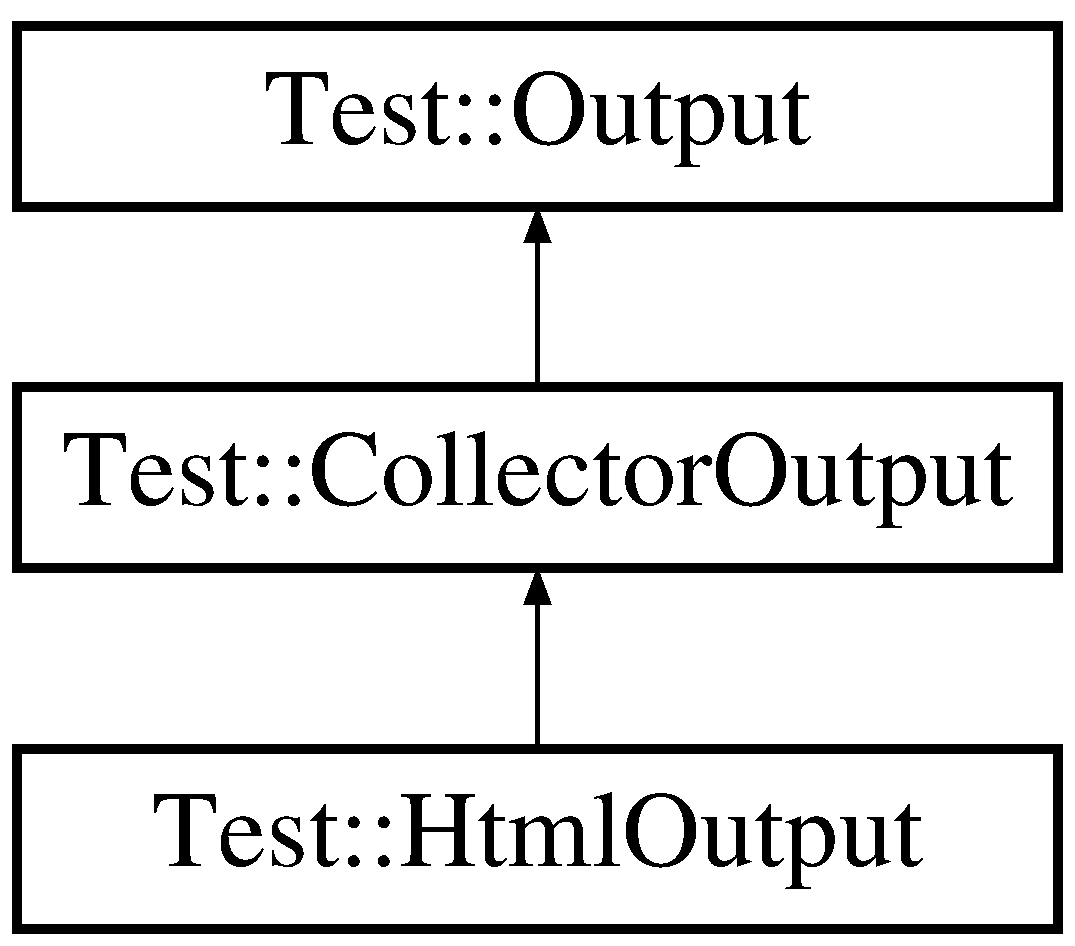
\includegraphics[height=3.000000cm]{class_test_1_1_html_output}
\end{center}
\end{figure}
\subsection*{Public Member Functions}
\begin{DoxyCompactItemize}
\item 
void \mbox{\hyperlink{class_test_1_1_html_output_a589e4e59aee4da0f70f3f6568daaf0f0}{generate}} (std\+::ostream \&os, bool incl\+\_\+ok\+\_\+tests=true, const std\+::string \&name=\char`\"{}\char`\"{})
\end{DoxyCompactItemize}
\subsection*{Friends}
\begin{DoxyCompactItemize}
\item 
struct \mbox{\hyperlink{class_test_1_1_html_output_a1e37e043f56a53b521955598f3366682}{Test\+Suite\+Row}}
\end{DoxyCompactItemize}
\subsection*{Additional Inherited Members}


\subsection{Detailed Description}
H\+T\+ML output. 

Output handler that creates a H\+T\+ML table with detailed information about all tests. 

Definition at line 44 of file cpptest-\/htmloutput.\+h.



\subsection{Member Function Documentation}
\mbox{\Hypertarget{class_test_1_1_html_output_a589e4e59aee4da0f70f3f6568daaf0f0}\label{class_test_1_1_html_output_a589e4e59aee4da0f70f3f6568daaf0f0}} 
\index{Test\+::\+Html\+Output@{Test\+::\+Html\+Output}!generate@{generate}}
\index{generate@{generate}!Test\+::\+Html\+Output@{Test\+::\+Html\+Output}}
\subsubsection{\texorpdfstring{generate()}{generate()}}
{\footnotesize\ttfamily void Test\+::\+Html\+Output\+::generate (\begin{DoxyParamCaption}\item[{std\+::ostream \&}]{os,  }\item[{bool}]{incl\+\_\+ok\+\_\+tests = {\ttfamily true},  }\item[{const std\+::string \&}]{name = {\ttfamily \char`\"{}\char`\"{}} }\end{DoxyParamCaption})}



\subsection{Friends And Related Function Documentation}
\mbox{\Hypertarget{class_test_1_1_html_output_a1e37e043f56a53b521955598f3366682}\label{class_test_1_1_html_output_a1e37e043f56a53b521955598f3366682}} 
\index{Test\+::\+Html\+Output@{Test\+::\+Html\+Output}!Test\+Suite\+Row@{Test\+Suite\+Row}}
\index{Test\+Suite\+Row@{Test\+Suite\+Row}!Test\+::\+Html\+Output@{Test\+::\+Html\+Output}}
\subsubsection{\texorpdfstring{Test\+Suite\+Row}{TestSuiteRow}}
{\footnotesize\ttfamily friend struct Test\+Suite\+Row\hspace{0.3cm}{\ttfamily [friend]}}



Definition at line 56 of file cpptest-\/htmloutput.\+h.



The documentation for this class was generated from the following file\+:\begin{DoxyCompactItemize}
\item 
\mbox{\hyperlink{cpptest-htmloutput_8h}{cpptest-\/htmloutput.\+h}}\end{DoxyCompactItemize}

\hypertarget{class_test_1_1_compiler_output_1_1_invalid_format}{}\section{Test\+:\+:Compiler\+Output\+:\+:Invalid\+Format Class Reference}
\label{class_test_1_1_compiler_output_1_1_invalid_format}\index{Test\+::\+Compiler\+Output\+::\+Invalid\+Format@{Test\+::\+Compiler\+Output\+::\+Invalid\+Format}}


Compiler output exception.  




{\ttfamily \#include $<$cpptest-\/compileroutput.\+h$>$}

Inheritance diagram for Test\+:\+:Compiler\+Output\+:\+:Invalid\+Format\+:\begin{figure}[H]
\begin{center}
\leavevmode
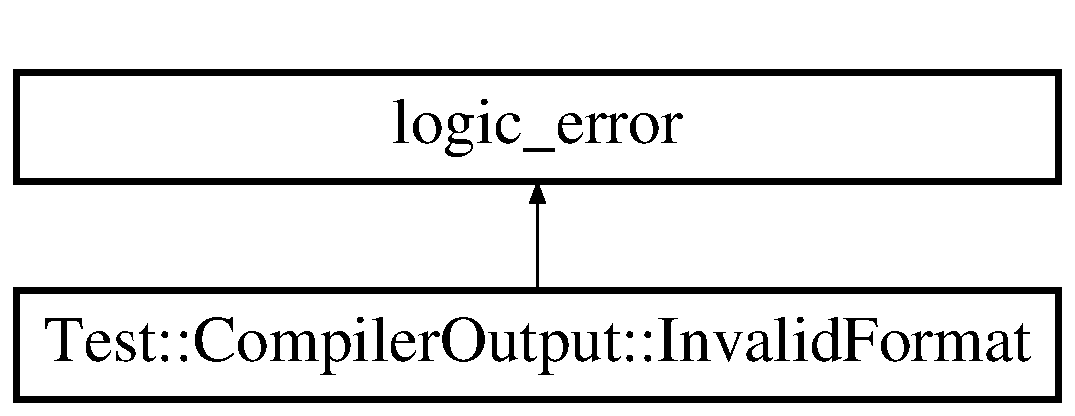
\includegraphics[height=2.000000cm]{class_test_1_1_compiler_output_1_1_invalid_format}
\end{center}
\end{figure}
\subsection*{Public Member Functions}
\begin{DoxyCompactItemize}
\item 
\mbox{\hyperlink{class_test_1_1_compiler_output_1_1_invalid_format_a3a7ab44239805bcefd4bc19c48c91992}{Invalid\+Format}} (const std\+::string \&what)
\end{DoxyCompactItemize}


\subsection{Detailed Description}
Compiler output exception. 

Indicates that an invalid message format was given when creating a compiler output. The failing format may be retrieved using the what() method. 

Definition at line 61 of file cpptest-\/compileroutput.\+h.



\subsection{Constructor \& Destructor Documentation}
\mbox{\Hypertarget{class_test_1_1_compiler_output_1_1_invalid_format_a3a7ab44239805bcefd4bc19c48c91992}\label{class_test_1_1_compiler_output_1_1_invalid_format_a3a7ab44239805bcefd4bc19c48c91992}} 
\index{Test\+::\+Compiler\+Output\+::\+Invalid\+Format@{Test\+::\+Compiler\+Output\+::\+Invalid\+Format}!Invalid\+Format@{Invalid\+Format}}
\index{Invalid\+Format@{Invalid\+Format}!Test\+::\+Compiler\+Output\+::\+Invalid\+Format@{Test\+::\+Compiler\+Output\+::\+Invalid\+Format}}
\subsubsection{\texorpdfstring{Invalid\+Format()}{InvalidFormat()}}
{\footnotesize\ttfamily Test\+::\+Compiler\+Output\+::\+Invalid\+Format\+::\+Invalid\+Format (\begin{DoxyParamCaption}\item[{const std\+::string \&}]{what }\end{DoxyParamCaption})\hspace{0.3cm}{\ttfamily [inline]}}



Definition at line 64 of file cpptest-\/compileroutput.\+h.



The documentation for this class was generated from the following file\+:\begin{DoxyCompactItemize}
\item 
\mbox{\hyperlink{cpptest-compileroutput_8h}{cpptest-\/compileroutput.\+h}}\end{DoxyCompactItemize}

\hypertarget{class_test_1_1_output}{}\section{Test\+:\+:Output Class Reference}
\label{class_test_1_1_output}\index{Test\+::\+Output@{Test\+::\+Output}}


Test suite output handler.  




{\ttfamily \#include $<$cpptest-\/output.\+h$>$}

Inheritance diagram for Test\+:\+:Output\+:\begin{figure}[H]
\begin{center}
\leavevmode
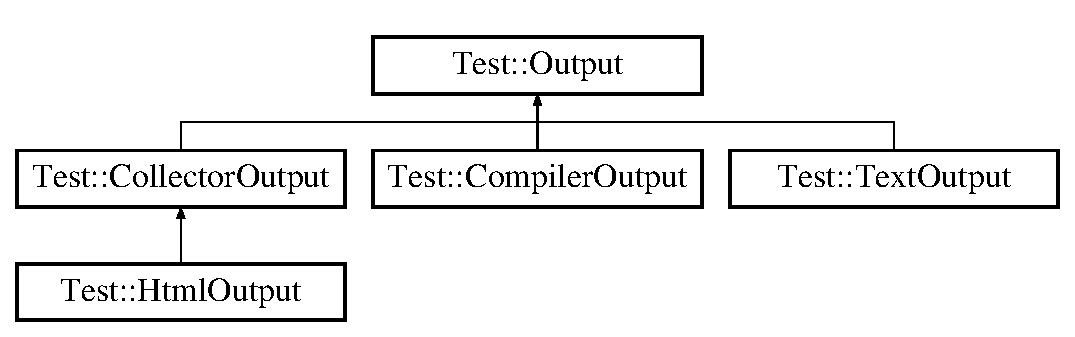
\includegraphics[height=3.000000cm]{class_test_1_1_output}
\end{center}
\end{figure}
\subsection*{Public Member Functions}
\begin{DoxyCompactItemize}
\item 
virtual \mbox{\hyperlink{class_test_1_1_output_a838de994609ac3d13b7d7cd389f56090}{$\sim$\+Output}} ()
\item 
virtual void \mbox{\hyperlink{class_test_1_1_output_aa66480875d088befc6c23ecfd1107cc1}{initialize}} (int tests)
\item 
virtual void \mbox{\hyperlink{class_test_1_1_output_aeff8af8326a8c54a38199f76837f860a}{finished}} (int tests, const \mbox{\hyperlink{class_test_1_1_time}{Time}} \&time)
\item 
virtual void \mbox{\hyperlink{class_test_1_1_output_a7022c32c5a1577b10b93d3942746f17d}{suite\+\_\+start}} (int tests, const std\+::string \&name)
\item 
virtual void \mbox{\hyperlink{class_test_1_1_output_a6dbf4c0adb2bd4a7364c629179f788a6}{suite\+\_\+end}} (int tests, const std\+::string \&name, const \mbox{\hyperlink{class_test_1_1_time}{Time}} \&time)
\item 
virtual void \mbox{\hyperlink{class_test_1_1_output_a52d43b97609febc5abbc6da9aa0abac2}{test\+\_\+start}} (const std\+::string \&name)
\item 
virtual void \mbox{\hyperlink{class_test_1_1_output_a3796943e3b56373492c957212a21454e}{test\+\_\+end}} (const std\+::string \&name, bool ok, const \mbox{\hyperlink{class_test_1_1_time}{Time}} \&time)
\item 
virtual void \mbox{\hyperlink{class_test_1_1_output_a48c31f0baa7627d81939be840c9a7f65}{assertment}} (const \mbox{\hyperlink{class_test_1_1_source}{Source}} \&s)
\end{DoxyCompactItemize}
\subsection*{Protected Member Functions}
\begin{DoxyCompactItemize}
\item 
\mbox{\hyperlink{class_test_1_1_output_acbffb6b160039caafd3e9ac11cace65c}{Output}} ()
\end{DoxyCompactItemize}


\subsection{Detailed Description}
Test suite output handler. 

Abstract base class for all suite output handlers. Derive from this class to create real output handlers that creates arbitrary complex output handlers.

All parts of testing is reported (test start/stop, suite start/stop, individual test start/stop, and assertments), thus giving maximum flexibility for derived classes. 

Definition at line 55 of file cpptest-\/output.\+h.



\subsection{Constructor \& Destructor Documentation}
\mbox{\Hypertarget{class_test_1_1_output_a838de994609ac3d13b7d7cd389f56090}\label{class_test_1_1_output_a838de994609ac3d13b7d7cd389f56090}} 
\index{Test\+::\+Output@{Test\+::\+Output}!````~Output@{$\sim$\+Output}}
\index{````~Output@{$\sim$\+Output}!Test\+::\+Output@{Test\+::\+Output}}
\subsubsection{\texorpdfstring{$\sim$\+Output()}{~Output()}}
{\footnotesize\ttfamily virtual Test\+::\+Output\+::$\sim$\+Output (\begin{DoxyParamCaption}{ }\end{DoxyParamCaption})\hspace{0.3cm}{\ttfamily [inline]}, {\ttfamily [virtual]}}

Empty destructor. 

Definition at line 60 of file cpptest-\/output.\+h.

\mbox{\Hypertarget{class_test_1_1_output_acbffb6b160039caafd3e9ac11cace65c}\label{class_test_1_1_output_acbffb6b160039caafd3e9ac11cace65c}} 
\index{Test\+::\+Output@{Test\+::\+Output}!Output@{Output}}
\index{Output@{Output}!Test\+::\+Output@{Test\+::\+Output}}
\subsubsection{\texorpdfstring{Output()}{Output()}}
{\footnotesize\ttfamily Test\+::\+Output\+::\+Output (\begin{DoxyParamCaption}{ }\end{DoxyParamCaption})\hspace{0.3cm}{\ttfamily [inline]}, {\ttfamily [protected]}}

Empty constructor. 

Definition at line 143 of file cpptest-\/output.\+h.



\subsection{Member Function Documentation}
\mbox{\Hypertarget{class_test_1_1_output_a48c31f0baa7627d81939be840c9a7f65}\label{class_test_1_1_output_a48c31f0baa7627d81939be840c9a7f65}} 
\index{Test\+::\+Output@{Test\+::\+Output}!assertment@{assertment}}
\index{assertment@{assertment}!Test\+::\+Output@{Test\+::\+Output}}
\subsubsection{\texorpdfstring{assertment()}{assertment()}}
{\footnotesize\ttfamily virtual void Test\+::\+Output\+::assertment (\begin{DoxyParamCaption}\item[{const \mbox{\hyperlink{class_test_1_1_source}{Source}} \&}]{s }\end{DoxyParamCaption})\hspace{0.3cm}{\ttfamily [inline]}, {\ttfamily [virtual]}}

Called when an assertment is issued.


\begin{DoxyParams}{Parameters}
{\em s} & Assert point information. \\
\hline
\end{DoxyParams}


Reimplemented in \mbox{\hyperlink{class_test_1_1_compiler_output_a1c36e3fd12afe3556e887349b0b86b50}{Test\+::\+Compiler\+Output}}, \mbox{\hyperlink{class_test_1_1_text_output_a8110f86aa00f783fc5a91ec2f59a7998}{Test\+::\+Text\+Output}}, and \mbox{\hyperlink{class_test_1_1_collector_output_a96b61d5e53c3dfa1b98747bb582aa4f3}{Test\+::\+Collector\+Output}}.



Definition at line 135 of file cpptest-\/output.\+h.

\mbox{\Hypertarget{class_test_1_1_output_aeff8af8326a8c54a38199f76837f860a}\label{class_test_1_1_output_aeff8af8326a8c54a38199f76837f860a}} 
\index{Test\+::\+Output@{Test\+::\+Output}!finished@{finished}}
\index{finished@{finished}!Test\+::\+Output@{Test\+::\+Output}}
\subsubsection{\texorpdfstring{finished()}{finished()}}
{\footnotesize\ttfamily virtual void Test\+::\+Output\+::finished (\begin{DoxyParamCaption}\item[{int}]{tests,  }\item[{const \mbox{\hyperlink{class_test_1_1_time}{Time}} \&}]{time }\end{DoxyParamCaption})\hspace{0.3cm}{\ttfamily [inline]}, {\ttfamily [virtual]}}

Called when testing is finished.


\begin{DoxyParams}{Parameters}
{\em tests} & Total number of tests in all suites. \\
\hline
{\em time} & Total elapsed time for all tests. \\
\hline
\end{DoxyParams}


Reimplemented in \mbox{\hyperlink{class_test_1_1_text_output_a9dcf13d9714a2774230386ef3215b701}{Test\+::\+Text\+Output}}, and \mbox{\hyperlink{class_test_1_1_collector_output_ad1a7502a31c58d93f0d88d7a679ab24d}{Test\+::\+Collector\+Output}}.



Definition at line 76 of file cpptest-\/output.\+h.

\mbox{\Hypertarget{class_test_1_1_output_aa66480875d088befc6c23ecfd1107cc1}\label{class_test_1_1_output_aa66480875d088befc6c23ecfd1107cc1}} 
\index{Test\+::\+Output@{Test\+::\+Output}!initialize@{initialize}}
\index{initialize@{initialize}!Test\+::\+Output@{Test\+::\+Output}}
\subsubsection{\texorpdfstring{initialize()}{initialize()}}
{\footnotesize\ttfamily virtual void Test\+::\+Output\+::initialize (\begin{DoxyParamCaption}\item[{int}]{tests }\end{DoxyParamCaption})\hspace{0.3cm}{\ttfamily [inline]}, {\ttfamily [virtual]}}

Called when testing is started.


\begin{DoxyParams}{Parameters}
{\em tests} & Total number of tests in all suites. \\
\hline
\end{DoxyParams}


Definition at line 66 of file cpptest-\/output.\+h.

\mbox{\Hypertarget{class_test_1_1_output_a6dbf4c0adb2bd4a7364c629179f788a6}\label{class_test_1_1_output_a6dbf4c0adb2bd4a7364c629179f788a6}} 
\index{Test\+::\+Output@{Test\+::\+Output}!suite\+\_\+end@{suite\+\_\+end}}
\index{suite\+\_\+end@{suite\+\_\+end}!Test\+::\+Output@{Test\+::\+Output}}
\subsubsection{\texorpdfstring{suite\+\_\+end()}{suite\_end()}}
{\footnotesize\ttfamily virtual void Test\+::\+Output\+::suite\+\_\+end (\begin{DoxyParamCaption}\item[{int}]{tests,  }\item[{const std\+::string \&}]{name,  }\item[{const \mbox{\hyperlink{class_test_1_1_time}{Time}} \&}]{time }\end{DoxyParamCaption})\hspace{0.3cm}{\ttfamily [inline]}, {\ttfamily [virtual]}}

Called when a suite is finished.


\begin{DoxyParams}{Parameters}
{\em tests} & Number of tests in this suite. \\
\hline
{\em name} & Name of the suite. \\
\hline
{\em time} & Total elapsed time for all tests in this suite. \\
\hline
\end{DoxyParams}


Reimplemented in \mbox{\hyperlink{class_test_1_1_text_output_a84efd3536702a815325590cc8837dbb2}{Test\+::\+Text\+Output}}, and \mbox{\hyperlink{class_test_1_1_collector_output_a50c041adf1de3e296b50b1611e55a407}{Test\+::\+Collector\+Output}}.



Definition at line 99 of file cpptest-\/output.\+h.

\mbox{\Hypertarget{class_test_1_1_output_a7022c32c5a1577b10b93d3942746f17d}\label{class_test_1_1_output_a7022c32c5a1577b10b93d3942746f17d}} 
\index{Test\+::\+Output@{Test\+::\+Output}!suite\+\_\+start@{suite\+\_\+start}}
\index{suite\+\_\+start@{suite\+\_\+start}!Test\+::\+Output@{Test\+::\+Output}}
\subsubsection{\texorpdfstring{suite\+\_\+start()}{suite\_start()}}
{\footnotesize\ttfamily virtual void Test\+::\+Output\+::suite\+\_\+start (\begin{DoxyParamCaption}\item[{int}]{tests,  }\item[{const std\+::string \&}]{name }\end{DoxyParamCaption})\hspace{0.3cm}{\ttfamily [inline]}, {\ttfamily [virtual]}}

Called when a suite is entered.


\begin{DoxyParams}{Parameters}
{\em tests} & Number of tests in this suite. \\
\hline
{\em name} & Name of the suite. \\
\hline
\end{DoxyParams}


Reimplemented in \mbox{\hyperlink{class_test_1_1_text_output_a0b6479918ee7f0501dfcdfcbc7c9d190}{Test\+::\+Text\+Output}}, and \mbox{\hyperlink{class_test_1_1_collector_output_a1d4c1eb5920fa96fb8dc8fe2eb0c336e}{Test\+::\+Collector\+Output}}.



Definition at line 87 of file cpptest-\/output.\+h.

\mbox{\Hypertarget{class_test_1_1_output_a3796943e3b56373492c957212a21454e}\label{class_test_1_1_output_a3796943e3b56373492c957212a21454e}} 
\index{Test\+::\+Output@{Test\+::\+Output}!test\+\_\+end@{test\+\_\+end}}
\index{test\+\_\+end@{test\+\_\+end}!Test\+::\+Output@{Test\+::\+Output}}
\subsubsection{\texorpdfstring{test\+\_\+end()}{test\_end()}}
{\footnotesize\ttfamily virtual void Test\+::\+Output\+::test\+\_\+end (\begin{DoxyParamCaption}\item[{const std\+::string \&}]{name,  }\item[{bool}]{ok,  }\item[{const \mbox{\hyperlink{class_test_1_1_time}{Time}} \&}]{time }\end{DoxyParamCaption})\hspace{0.3cm}{\ttfamily [inline]}, {\ttfamily [virtual]}}

Called when a test if finished, regardless if an assertment was issued.


\begin{DoxyParams}{Parameters}
{\em name} & Name of the test function. \\
\hline
{\em ok} & True if the test was successful; false otherwise. \\
\hline
{\em time} & Execution time. \\
\hline
\end{DoxyParams}


Reimplemented in \mbox{\hyperlink{class_test_1_1_text_output_a0ff333537e85d680740c72dd46cd2e7e}{Test\+::\+Text\+Output}}, and \mbox{\hyperlink{class_test_1_1_collector_output_a08aa350c9a0ce221d03f6841a0b5d633}{Test\+::\+Collector\+Output}}.



Definition at line 123 of file cpptest-\/output.\+h.

\mbox{\Hypertarget{class_test_1_1_output_a52d43b97609febc5abbc6da9aa0abac2}\label{class_test_1_1_output_a52d43b97609febc5abbc6da9aa0abac2}} 
\index{Test\+::\+Output@{Test\+::\+Output}!test\+\_\+start@{test\+\_\+start}}
\index{test\+\_\+start@{test\+\_\+start}!Test\+::\+Output@{Test\+::\+Output}}
\subsubsection{\texorpdfstring{test\+\_\+start()}{test\_start()}}
{\footnotesize\ttfamily virtual void Test\+::\+Output\+::test\+\_\+start (\begin{DoxyParamCaption}\item[{const std\+::string \&}]{name }\end{DoxyParamCaption})\hspace{0.3cm}{\ttfamily [inline]}, {\ttfamily [virtual]}}

Called when a tests is executed.


\begin{DoxyParams}{Parameters}
{\em name} & Name of the test function. \\
\hline
\end{DoxyParams}


Reimplemented in \mbox{\hyperlink{class_test_1_1_collector_output_a0ac72b71fac68305ceabb1c516760eb0}{Test\+::\+Collector\+Output}}.



Definition at line 111 of file cpptest-\/output.\+h.



The documentation for this class was generated from the following file\+:\begin{DoxyCompactItemize}
\item 
\mbox{\hyperlink{cpptest-output_8h}{cpptest-\/output.\+h}}\end{DoxyCompactItemize}

\hypertarget{class_record_processor}{}\section{Record\+Processor Class Reference}
\label{class_record_processor}\index{Record\+Processor@{Record\+Processor}}


{\ttfamily \#include $<$Record\+Processor.\+h$>$}

\subsection*{Public Member Functions}
\begin{DoxyCompactItemize}
\item 
\mbox{\hyperlink{class_record_processor_a3961a0d77a0d83e58a68736311b88a0a}{Record\+Processor}} ()
\item 
\mbox{\hyperlink{class_record_processor_aa64ac5cbddceb678e8cb27e9fc58576c}{Record\+Processor}} (const char $\ast$filename)
\item 
bool \mbox{\hyperlink{class_record_processor_a2c919a73f9cd411c141635f35dd047be}{create\+Table}} ()
\item 
bool \mbox{\hyperlink{class_record_processor_a6739098423e2d913004459282217db2e}{delete\+Table}} ()
\item 
bool \mbox{\hyperlink{class_record_processor_a6101b13cf5883e1fefe3013947ca9b68}{insert\+Record}} (const char $\ast$sql)
\item 
\mbox{\hyperlink{_record_processor_8h_a38f4f71143d55126a9f66fd1f9824999}{Records}} \& \mbox{\hyperlink{class_record_processor_aa246f2377aaba5ade7524813f07eaec0}{select\+Record}} (const char $\ast$sql)
\item 
\mbox{\hyperlink{class_record_processor_a63fbf98c72bafa6c2e24a3962bdae70c}{$\sim$\+Record\+Processor}} ()
\end{DoxyCompactItemize}


\subsection{Detailed Description}


Definition at line 17 of file Record\+Processor.\+h.



\subsection{Constructor \& Destructor Documentation}
\mbox{\Hypertarget{class_record_processor_a3961a0d77a0d83e58a68736311b88a0a}\label{class_record_processor_a3961a0d77a0d83e58a68736311b88a0a}} 
\index{Record\+Processor@{Record\+Processor}!Record\+Processor@{Record\+Processor}}
\index{Record\+Processor@{Record\+Processor}!Record\+Processor@{Record\+Processor}}
\subsubsection{\texorpdfstring{Record\+Processor()}{RecordProcessor()}\hspace{0.1cm}{\footnotesize\ttfamily [1/2]}}
{\footnotesize\ttfamily Record\+Processor\+::\+Record\+Processor (\begin{DoxyParamCaption}{ }\end{DoxyParamCaption})}



Definition at line 67 of file Record\+Processor.\+cpp.

\mbox{\Hypertarget{class_record_processor_aa64ac5cbddceb678e8cb27e9fc58576c}\label{class_record_processor_aa64ac5cbddceb678e8cb27e9fc58576c}} 
\index{Record\+Processor@{Record\+Processor}!Record\+Processor@{Record\+Processor}}
\index{Record\+Processor@{Record\+Processor}!Record\+Processor@{Record\+Processor}}
\subsubsection{\texorpdfstring{Record\+Processor()}{RecordProcessor()}\hspace{0.1cm}{\footnotesize\ttfamily [2/2]}}
{\footnotesize\ttfamily Record\+Processor\+::\+Record\+Processor (\begin{DoxyParamCaption}\item[{const char $\ast$}]{filename }\end{DoxyParamCaption})}



Definition at line 84 of file Record\+Processor.\+cpp.

\mbox{\Hypertarget{class_record_processor_a63fbf98c72bafa6c2e24a3962bdae70c}\label{class_record_processor_a63fbf98c72bafa6c2e24a3962bdae70c}} 
\index{Record\+Processor@{Record\+Processor}!````~Record\+Processor@{$\sim$\+Record\+Processor}}
\index{````~Record\+Processor@{$\sim$\+Record\+Processor}!Record\+Processor@{Record\+Processor}}
\subsubsection{\texorpdfstring{$\sim$\+Record\+Processor()}{~RecordProcessor()}}
{\footnotesize\ttfamily Record\+Processor\+::$\sim$\+Record\+Processor (\begin{DoxyParamCaption}{ }\end{DoxyParamCaption})}



Definition at line 180 of file Record\+Processor.\+cpp.



\subsection{Member Function Documentation}
\mbox{\Hypertarget{class_record_processor_a2c919a73f9cd411c141635f35dd047be}\label{class_record_processor_a2c919a73f9cd411c141635f35dd047be}} 
\index{Record\+Processor@{Record\+Processor}!create\+Table@{create\+Table}}
\index{create\+Table@{create\+Table}!Record\+Processor@{Record\+Processor}}
\subsubsection{\texorpdfstring{create\+Table()}{createTable()}}
{\footnotesize\ttfamily bool Record\+Processor\+::create\+Table (\begin{DoxyParamCaption}{ }\end{DoxyParamCaption})}



Definition at line 100 of file Record\+Processor.\+cpp.

\mbox{\Hypertarget{class_record_processor_a6739098423e2d913004459282217db2e}\label{class_record_processor_a6739098423e2d913004459282217db2e}} 
\index{Record\+Processor@{Record\+Processor}!delete\+Table@{delete\+Table}}
\index{delete\+Table@{delete\+Table}!Record\+Processor@{Record\+Processor}}
\subsubsection{\texorpdfstring{delete\+Table()}{deleteTable()}}
{\footnotesize\ttfamily bool Record\+Processor\+::delete\+Table (\begin{DoxyParamCaption}{ }\end{DoxyParamCaption})}



Definition at line 123 of file Record\+Processor.\+cpp.

\mbox{\Hypertarget{class_record_processor_a6101b13cf5883e1fefe3013947ca9b68}\label{class_record_processor_a6101b13cf5883e1fefe3013947ca9b68}} 
\index{Record\+Processor@{Record\+Processor}!insert\+Record@{insert\+Record}}
\index{insert\+Record@{insert\+Record}!Record\+Processor@{Record\+Processor}}
\subsubsection{\texorpdfstring{insert\+Record()}{insertRecord()}}
{\footnotesize\ttfamily bool Record\+Processor\+::insert\+Record (\begin{DoxyParamCaption}\item[{const char $\ast$}]{sql }\end{DoxyParamCaption})}



Definition at line 143 of file Record\+Processor.\+cpp.

\mbox{\Hypertarget{class_record_processor_aa246f2377aaba5ade7524813f07eaec0}\label{class_record_processor_aa246f2377aaba5ade7524813f07eaec0}} 
\index{Record\+Processor@{Record\+Processor}!select\+Record@{select\+Record}}
\index{select\+Record@{select\+Record}!Record\+Processor@{Record\+Processor}}
\subsubsection{\texorpdfstring{select\+Record()}{selectRecord()}}
{\footnotesize\ttfamily \mbox{\hyperlink{_record_processor_8h_a38f4f71143d55126a9f66fd1f9824999}{Records}} \& Record\+Processor\+::select\+Record (\begin{DoxyParamCaption}\item[{const char $\ast$}]{sql }\end{DoxyParamCaption})}



Definition at line 159 of file Record\+Processor.\+cpp.



The documentation for this class was generated from the following files\+:\begin{DoxyCompactItemize}
\item 
\mbox{\hyperlink{_record_processor_8h}{Record\+Processor.\+h}}\item 
\mbox{\hyperlink{_record_processor_8cpp}{Record\+Processor.\+cpp}}\end{DoxyCompactItemize}

\hypertarget{class_test_1_1_source}{}\section{Test\+:\+:Source Class Reference}
\label{class_test_1_1_source}\index{Test\+::\+Source@{Test\+::\+Source}}


Assertment source information.  




{\ttfamily \#include $<$cpptest-\/source.\+h$>$}

\subsection*{Public Member Functions}
\begin{DoxyCompactItemize}
\item 
\mbox{\hyperlink{class_test_1_1_source_abe0f303fe92270aa12a4a749ae0395ef}{Source}} ()
\item 
\mbox{\hyperlink{class_test_1_1_source_ac764beb685a574b81527d0f90ae9e428}{Source}} (const char $\ast$\mbox{\hyperlink{class_test_1_1_source_a5244b21c0aae95eab1c87f69ab108a2d}{file}}, unsigned int \mbox{\hyperlink{class_test_1_1_source_ae3da8b65a4a950a4be76bae056dbb5ee}{line}}, const char $\ast$msg)
\item 
const std\+::string \& \mbox{\hyperlink{class_test_1_1_source_a5244b21c0aae95eab1c87f69ab108a2d}{file}} () const
\item 
unsigned int \mbox{\hyperlink{class_test_1_1_source_ae3da8b65a4a950a4be76bae056dbb5ee}{line}} () const
\item 
const std\+::string \& \mbox{\hyperlink{class_test_1_1_source_add142dd87973b9b16dfad92ba1efbe9c}{message}} () const
\item 
const std\+::string \& \mbox{\hyperlink{class_test_1_1_source_afb6c58ea7325e7082539f4e1cefc4508}{suite}} () const
\item 
const std\+::string \& \mbox{\hyperlink{class_test_1_1_source_a7f4861f56448910101a61d4e3c1c471f}{test}} () const
\end{DoxyCompactItemize}
\subsection*{Friends}
\begin{DoxyCompactItemize}
\item 
class \mbox{\hyperlink{class_test_1_1_source_a7de7b0dd89982bdae285f3a3b6197f9c}{Suite}}
\end{DoxyCompactItemize}


\subsection{Detailed Description}
Assertment source information. 

Contains information about an assertment point. 

Definition at line 42 of file cpptest-\/source.\+h.



\subsection{Constructor \& Destructor Documentation}
\mbox{\Hypertarget{class_test_1_1_source_abe0f303fe92270aa12a4a749ae0395ef}\label{class_test_1_1_source_abe0f303fe92270aa12a4a749ae0395ef}} 
\index{Test\+::\+Source@{Test\+::\+Source}!Source@{Source}}
\index{Source@{Source}!Test\+::\+Source@{Test\+::\+Source}}
\subsubsection{\texorpdfstring{Source()}{Source()}\hspace{0.1cm}{\footnotesize\ttfamily [1/2]}}
{\footnotesize\ttfamily Test\+::\+Source\+::\+Source (\begin{DoxyParamCaption}{ }\end{DoxyParamCaption})}

\mbox{\Hypertarget{class_test_1_1_source_ac764beb685a574b81527d0f90ae9e428}\label{class_test_1_1_source_ac764beb685a574b81527d0f90ae9e428}} 
\index{Test\+::\+Source@{Test\+::\+Source}!Source@{Source}}
\index{Source@{Source}!Test\+::\+Source@{Test\+::\+Source}}
\subsubsection{\texorpdfstring{Source()}{Source()}\hspace{0.1cm}{\footnotesize\ttfamily [2/2]}}
{\footnotesize\ttfamily Test\+::\+Source\+::\+Source (\begin{DoxyParamCaption}\item[{const char $\ast$}]{file,  }\item[{unsigned int}]{line,  }\item[{const char $\ast$}]{msg }\end{DoxyParamCaption})}



\subsection{Member Function Documentation}
\mbox{\Hypertarget{class_test_1_1_source_a5244b21c0aae95eab1c87f69ab108a2d}\label{class_test_1_1_source_a5244b21c0aae95eab1c87f69ab108a2d}} 
\index{Test\+::\+Source@{Test\+::\+Source}!file@{file}}
\index{file@{file}!Test\+::\+Source@{Test\+::\+Source}}
\subsubsection{\texorpdfstring{file()}{file()}}
{\footnotesize\ttfamily const std\+::string\& Test\+::\+Source\+::file (\begin{DoxyParamCaption}{ }\end{DoxyParamCaption}) const}

\mbox{\Hypertarget{class_test_1_1_source_ae3da8b65a4a950a4be76bae056dbb5ee}\label{class_test_1_1_source_ae3da8b65a4a950a4be76bae056dbb5ee}} 
\index{Test\+::\+Source@{Test\+::\+Source}!line@{line}}
\index{line@{line}!Test\+::\+Source@{Test\+::\+Source}}
\subsubsection{\texorpdfstring{line()}{line()}}
{\footnotesize\ttfamily unsigned int Test\+::\+Source\+::line (\begin{DoxyParamCaption}{ }\end{DoxyParamCaption}) const}

\mbox{\Hypertarget{class_test_1_1_source_add142dd87973b9b16dfad92ba1efbe9c}\label{class_test_1_1_source_add142dd87973b9b16dfad92ba1efbe9c}} 
\index{Test\+::\+Source@{Test\+::\+Source}!message@{message}}
\index{message@{message}!Test\+::\+Source@{Test\+::\+Source}}
\subsubsection{\texorpdfstring{message()}{message()}}
{\footnotesize\ttfamily const std\+::string\& Test\+::\+Source\+::message (\begin{DoxyParamCaption}{ }\end{DoxyParamCaption}) const}

\mbox{\Hypertarget{class_test_1_1_source_afb6c58ea7325e7082539f4e1cefc4508}\label{class_test_1_1_source_afb6c58ea7325e7082539f4e1cefc4508}} 
\index{Test\+::\+Source@{Test\+::\+Source}!suite@{suite}}
\index{suite@{suite}!Test\+::\+Source@{Test\+::\+Source}}
\subsubsection{\texorpdfstring{suite()}{suite()}}
{\footnotesize\ttfamily const std\+::string\& Test\+::\+Source\+::suite (\begin{DoxyParamCaption}{ }\end{DoxyParamCaption}) const}

\mbox{\Hypertarget{class_test_1_1_source_a7f4861f56448910101a61d4e3c1c471f}\label{class_test_1_1_source_a7f4861f56448910101a61d4e3c1c471f}} 
\index{Test\+::\+Source@{Test\+::\+Source}!test@{test}}
\index{test@{test}!Test\+::\+Source@{Test\+::\+Source}}
\subsubsection{\texorpdfstring{test()}{test()}}
{\footnotesize\ttfamily const std\+::string\& Test\+::\+Source\+::test (\begin{DoxyParamCaption}{ }\end{DoxyParamCaption}) const}



\subsection{Friends And Related Function Documentation}
\mbox{\Hypertarget{class_test_1_1_source_a7de7b0dd89982bdae285f3a3b6197f9c}\label{class_test_1_1_source_a7de7b0dd89982bdae285f3a3b6197f9c}} 
\index{Test\+::\+Source@{Test\+::\+Source}!Suite@{Suite}}
\index{Suite@{Suite}!Test\+::\+Source@{Test\+::\+Source}}
\subsubsection{\texorpdfstring{Suite}{Suite}}
{\footnotesize\ttfamily friend class \mbox{\hyperlink{class_test_1_1_suite}{Suite}}\hspace{0.3cm}{\ttfamily [friend]}}



Definition at line 44 of file cpptest-\/source.\+h.



The documentation for this class was generated from the following file\+:\begin{DoxyCompactItemize}
\item 
\mbox{\hyperlink{cpptest-source_8h}{cpptest-\/source.\+h}}\end{DoxyCompactItemize}

\hypertarget{structsqlite3__file}{}\section{sqlite3\+\_\+file Struct Reference}
\label{structsqlite3__file}\index{sqlite3\+\_\+file@{sqlite3\+\_\+file}}


{\ttfamily \#include $<$sqlite3.\+h$>$}

\subsection*{Public Attributes}
\begin{DoxyCompactItemize}
\item 
const struct \mbox{\hyperlink{structsqlite3__io__methods}{sqlite3\+\_\+io\+\_\+methods}} $\ast$ \mbox{\hyperlink{structsqlite3__file_adfc58b2d7514112375d7330e2881bc70}{p\+Methods}}
\end{DoxyCompactItemize}


\subsection{Detailed Description}


Definition at line 667 of file sqlite3.\+h.



\subsection{Member Data Documentation}
\mbox{\Hypertarget{structsqlite3__file_adfc58b2d7514112375d7330e2881bc70}\label{structsqlite3__file_adfc58b2d7514112375d7330e2881bc70}} 
\index{sqlite3\+\_\+file@{sqlite3\+\_\+file}!p\+Methods@{p\+Methods}}
\index{p\+Methods@{p\+Methods}!sqlite3\+\_\+file@{sqlite3\+\_\+file}}
\subsubsection{\texorpdfstring{p\+Methods}{pMethods}}
{\footnotesize\ttfamily const struct \mbox{\hyperlink{structsqlite3__io__methods}{sqlite3\+\_\+io\+\_\+methods}}$\ast$ sqlite3\+\_\+file\+::p\+Methods}



Definition at line 668 of file sqlite3.\+h.



The documentation for this struct was generated from the following file\+:\begin{DoxyCompactItemize}
\item 
\mbox{\hyperlink{sqlite3_8h}{sqlite3.\+h}}\end{DoxyCompactItemize}

\hypertarget{structsqlite3__index__info_1_1sqlite3__index__constraint}{}\section{sqlite3\+\_\+index\+\_\+info\+:\+:sqlite3\+\_\+index\+\_\+constraint Struct Reference}
\label{structsqlite3__index__info_1_1sqlite3__index__constraint}\index{sqlite3\+\_\+index\+\_\+info\+::sqlite3\+\_\+index\+\_\+constraint@{sqlite3\+\_\+index\+\_\+info\+::sqlite3\+\_\+index\+\_\+constraint}}


{\ttfamily \#include $<$sqlite3.\+h$>$}

\subsection*{Public Attributes}
\begin{DoxyCompactItemize}
\item 
int \mbox{\hyperlink{structsqlite3__index__info_1_1sqlite3__index__constraint_a0f1e207060420058ee2881f2ea368e3a}{i\+Column}}
\item 
unsigned char \mbox{\hyperlink{structsqlite3__index__info_1_1sqlite3__index__constraint_a362f4ec1f71975cb0ac39a8b5e4b1476}{op}}
\item 
unsigned char \mbox{\hyperlink{structsqlite3__index__info_1_1sqlite3__index__constraint_ae16e62caeab743cc68bb22227dacb501}{usable}}
\item 
int \mbox{\hyperlink{structsqlite3__index__info_1_1sqlite3__index__constraint_a4e8368da66f34b7f07b369984b813d1b}{i\+Term\+Offset}}
\end{DoxyCompactItemize}


\subsection{Detailed Description}


Definition at line 6208 of file sqlite3.\+h.



\subsection{Member Data Documentation}
\mbox{\Hypertarget{structsqlite3__index__info_1_1sqlite3__index__constraint_a0f1e207060420058ee2881f2ea368e3a}\label{structsqlite3__index__info_1_1sqlite3__index__constraint_a0f1e207060420058ee2881f2ea368e3a}} 
\index{sqlite3\+\_\+index\+\_\+info\+::sqlite3\+\_\+index\+\_\+constraint@{sqlite3\+\_\+index\+\_\+info\+::sqlite3\+\_\+index\+\_\+constraint}!i\+Column@{i\+Column}}
\index{i\+Column@{i\+Column}!sqlite3\+\_\+index\+\_\+info\+::sqlite3\+\_\+index\+\_\+constraint@{sqlite3\+\_\+index\+\_\+info\+::sqlite3\+\_\+index\+\_\+constraint}}
\subsubsection{\texorpdfstring{i\+Column}{iColumn}}
{\footnotesize\ttfamily int sqlite3\+\_\+index\+\_\+info\+::sqlite3\+\_\+index\+\_\+constraint\+::i\+Column}



Definition at line 6209 of file sqlite3.\+h.

\mbox{\Hypertarget{structsqlite3__index__info_1_1sqlite3__index__constraint_a4e8368da66f34b7f07b369984b813d1b}\label{structsqlite3__index__info_1_1sqlite3__index__constraint_a4e8368da66f34b7f07b369984b813d1b}} 
\index{sqlite3\+\_\+index\+\_\+info\+::sqlite3\+\_\+index\+\_\+constraint@{sqlite3\+\_\+index\+\_\+info\+::sqlite3\+\_\+index\+\_\+constraint}!i\+Term\+Offset@{i\+Term\+Offset}}
\index{i\+Term\+Offset@{i\+Term\+Offset}!sqlite3\+\_\+index\+\_\+info\+::sqlite3\+\_\+index\+\_\+constraint@{sqlite3\+\_\+index\+\_\+info\+::sqlite3\+\_\+index\+\_\+constraint}}
\subsubsection{\texorpdfstring{i\+Term\+Offset}{iTermOffset}}
{\footnotesize\ttfamily int sqlite3\+\_\+index\+\_\+info\+::sqlite3\+\_\+index\+\_\+constraint\+::i\+Term\+Offset}



Definition at line 6212 of file sqlite3.\+h.

\mbox{\Hypertarget{structsqlite3__index__info_1_1sqlite3__index__constraint_a362f4ec1f71975cb0ac39a8b5e4b1476}\label{structsqlite3__index__info_1_1sqlite3__index__constraint_a362f4ec1f71975cb0ac39a8b5e4b1476}} 
\index{sqlite3\+\_\+index\+\_\+info\+::sqlite3\+\_\+index\+\_\+constraint@{sqlite3\+\_\+index\+\_\+info\+::sqlite3\+\_\+index\+\_\+constraint}!op@{op}}
\index{op@{op}!sqlite3\+\_\+index\+\_\+info\+::sqlite3\+\_\+index\+\_\+constraint@{sqlite3\+\_\+index\+\_\+info\+::sqlite3\+\_\+index\+\_\+constraint}}
\subsubsection{\texorpdfstring{op}{op}}
{\footnotesize\ttfamily unsigned char sqlite3\+\_\+index\+\_\+info\+::sqlite3\+\_\+index\+\_\+constraint\+::op}



Definition at line 6210 of file sqlite3.\+h.

\mbox{\Hypertarget{structsqlite3__index__info_1_1sqlite3__index__constraint_ae16e62caeab743cc68bb22227dacb501}\label{structsqlite3__index__info_1_1sqlite3__index__constraint_ae16e62caeab743cc68bb22227dacb501}} 
\index{sqlite3\+\_\+index\+\_\+info\+::sqlite3\+\_\+index\+\_\+constraint@{sqlite3\+\_\+index\+\_\+info\+::sqlite3\+\_\+index\+\_\+constraint}!usable@{usable}}
\index{usable@{usable}!sqlite3\+\_\+index\+\_\+info\+::sqlite3\+\_\+index\+\_\+constraint@{sqlite3\+\_\+index\+\_\+info\+::sqlite3\+\_\+index\+\_\+constraint}}
\subsubsection{\texorpdfstring{usable}{usable}}
{\footnotesize\ttfamily unsigned char sqlite3\+\_\+index\+\_\+info\+::sqlite3\+\_\+index\+\_\+constraint\+::usable}



Definition at line 6211 of file sqlite3.\+h.



The documentation for this struct was generated from the following file\+:\begin{DoxyCompactItemize}
\item 
\mbox{\hyperlink{sqlite3_8h}{sqlite3.\+h}}\end{DoxyCompactItemize}

\hypertarget{structsqlite3__index__info_1_1sqlite3__index__constraint__usage}{}\section{sqlite3\+\_\+index\+\_\+info\+:\+:sqlite3\+\_\+index\+\_\+constraint\+\_\+usage Struct Reference}
\label{structsqlite3__index__info_1_1sqlite3__index__constraint__usage}\index{sqlite3\+\_\+index\+\_\+info\+::sqlite3\+\_\+index\+\_\+constraint\+\_\+usage@{sqlite3\+\_\+index\+\_\+info\+::sqlite3\+\_\+index\+\_\+constraint\+\_\+usage}}


{\ttfamily \#include $<$sqlite3.\+h$>$}

\subsection*{Public Attributes}
\begin{DoxyCompactItemize}
\item 
int \mbox{\hyperlink{structsqlite3__index__info_1_1sqlite3__index__constraint__usage_a2cbf680033c2937b3de226e091743a94}{argv\+Index}}
\item 
unsigned char \mbox{\hyperlink{structsqlite3__index__info_1_1sqlite3__index__constraint__usage_ad07fa17d30e4fb3abe23ceaf84edf0ef}{omit}}
\end{DoxyCompactItemize}


\subsection{Detailed Description}


Definition at line 6220 of file sqlite3.\+h.



\subsection{Member Data Documentation}
\mbox{\Hypertarget{structsqlite3__index__info_1_1sqlite3__index__constraint__usage_a2cbf680033c2937b3de226e091743a94}\label{structsqlite3__index__info_1_1sqlite3__index__constraint__usage_a2cbf680033c2937b3de226e091743a94}} 
\index{sqlite3\+\_\+index\+\_\+info\+::sqlite3\+\_\+index\+\_\+constraint\+\_\+usage@{sqlite3\+\_\+index\+\_\+info\+::sqlite3\+\_\+index\+\_\+constraint\+\_\+usage}!argv\+Index@{argv\+Index}}
\index{argv\+Index@{argv\+Index}!sqlite3\+\_\+index\+\_\+info\+::sqlite3\+\_\+index\+\_\+constraint\+\_\+usage@{sqlite3\+\_\+index\+\_\+info\+::sqlite3\+\_\+index\+\_\+constraint\+\_\+usage}}
\subsubsection{\texorpdfstring{argv\+Index}{argvIndex}}
{\footnotesize\ttfamily int sqlite3\+\_\+index\+\_\+info\+::sqlite3\+\_\+index\+\_\+constraint\+\_\+usage\+::argv\+Index}



Definition at line 6221 of file sqlite3.\+h.

\mbox{\Hypertarget{structsqlite3__index__info_1_1sqlite3__index__constraint__usage_ad07fa17d30e4fb3abe23ceaf84edf0ef}\label{structsqlite3__index__info_1_1sqlite3__index__constraint__usage_ad07fa17d30e4fb3abe23ceaf84edf0ef}} 
\index{sqlite3\+\_\+index\+\_\+info\+::sqlite3\+\_\+index\+\_\+constraint\+\_\+usage@{sqlite3\+\_\+index\+\_\+info\+::sqlite3\+\_\+index\+\_\+constraint\+\_\+usage}!omit@{omit}}
\index{omit@{omit}!sqlite3\+\_\+index\+\_\+info\+::sqlite3\+\_\+index\+\_\+constraint\+\_\+usage@{sqlite3\+\_\+index\+\_\+info\+::sqlite3\+\_\+index\+\_\+constraint\+\_\+usage}}
\subsubsection{\texorpdfstring{omit}{omit}}
{\footnotesize\ttfamily unsigned char sqlite3\+\_\+index\+\_\+info\+::sqlite3\+\_\+index\+\_\+constraint\+\_\+usage\+::omit}



Definition at line 6222 of file sqlite3.\+h.



The documentation for this struct was generated from the following file\+:\begin{DoxyCompactItemize}
\item 
\mbox{\hyperlink{sqlite3_8h}{sqlite3.\+h}}\end{DoxyCompactItemize}

\hypertarget{structsqlite3__index__info}{}\section{sqlite3\+\_\+index\+\_\+info Struct Reference}
\label{structsqlite3__index__info}\index{sqlite3\+\_\+index\+\_\+info@{sqlite3\+\_\+index\+\_\+info}}


{\ttfamily \#include $<$sqlite3.\+h$>$}

\subsection*{Classes}
\begin{DoxyCompactItemize}
\item 
struct \mbox{\hyperlink{structsqlite3__index__info_1_1sqlite3__index__constraint}{sqlite3\+\_\+index\+\_\+constraint}}
\item 
struct \mbox{\hyperlink{structsqlite3__index__info_1_1sqlite3__index__constraint__usage}{sqlite3\+\_\+index\+\_\+constraint\+\_\+usage}}
\item 
struct \mbox{\hyperlink{structsqlite3__index__info_1_1sqlite3__index__orderby}{sqlite3\+\_\+index\+\_\+orderby}}
\end{DoxyCompactItemize}
\subsection*{Public Attributes}
\begin{DoxyCompactItemize}
\item 
int \mbox{\hyperlink{structsqlite3__index__info_ae861993a30ce914a5214eab2579d935a}{n\+Constraint}}
\item 
struct \mbox{\hyperlink{structsqlite3__index__info_1_1sqlite3__index__constraint}{sqlite3\+\_\+index\+\_\+info\+::sqlite3\+\_\+index\+\_\+constraint}} $\ast$ \mbox{\hyperlink{structsqlite3__index__info_a634aa93834e2b47acf34454746c0f248}{a\+Constraint}}
\item 
int \mbox{\hyperlink{structsqlite3__index__info_a3ef850fdc57eddbc8189fe84d0a9044e}{n\+Order\+By}}
\item 
struct \mbox{\hyperlink{structsqlite3__index__info_1_1sqlite3__index__orderby}{sqlite3\+\_\+index\+\_\+info\+::sqlite3\+\_\+index\+\_\+orderby}} $\ast$ \mbox{\hyperlink{structsqlite3__index__info_a6823a68979e19d8e332389361e920ef9}{a\+Order\+By}}
\item 
struct \mbox{\hyperlink{structsqlite3__index__info_1_1sqlite3__index__constraint__usage}{sqlite3\+\_\+index\+\_\+info\+::sqlite3\+\_\+index\+\_\+constraint\+\_\+usage}} $\ast$ \mbox{\hyperlink{structsqlite3__index__info_a79b8a969dd7d582fc2ea3c0fbc5adb56}{a\+Constraint\+Usage}}
\item 
int \mbox{\hyperlink{structsqlite3__index__info_afcee17707a1c147fbd55c23c807fdae3}{idx\+Num}}
\item 
char $\ast$ \mbox{\hyperlink{structsqlite3__index__info_a1a9935e997bd6e3cce048534da7506a7}{idx\+Str}}
\item 
int \mbox{\hyperlink{structsqlite3__index__info_a5410066c067c3891cdf165c70cc4d6b1}{need\+To\+Free\+Idx\+Str}}
\item 
int \mbox{\hyperlink{structsqlite3__index__info_a5515d9de0f37f68d7e0930c20a668b29}{order\+By\+Consumed}}
\item 
double \mbox{\hyperlink{structsqlite3__index__info_aa8b4fe1d2ee38aab57ba5e1da00d7830}{estimated\+Cost}}
\item 
\mbox{\hyperlink{sqlite3_8h_a0a4d3e6c1ad46f90e746b920ab6ca0d2}{sqlite3\+\_\+int64}} \mbox{\hyperlink{structsqlite3__index__info_adcdf25dcf9848a6fedf539bb9c921b7f}{estimated\+Rows}}
\item 
int \mbox{\hyperlink{structsqlite3__index__info_a8acf2a7efbc3e193cf01d2afbd44fdbb}{idx\+Flags}}
\item 
\mbox{\hyperlink{sqlite3_8h_a181c20ecfd72bc6627635746d382c610}{sqlite3\+\_\+uint64}} \mbox{\hyperlink{structsqlite3__index__info_a99787169e2f78c0728bdb339c4107a2e}{col\+Used}}
\end{DoxyCompactItemize}


\subsection{Detailed Description}


Definition at line 6205 of file sqlite3.\+h.



\subsection{Member Data Documentation}
\mbox{\Hypertarget{structsqlite3__index__info_a634aa93834e2b47acf34454746c0f248}\label{structsqlite3__index__info_a634aa93834e2b47acf34454746c0f248}} 
\index{sqlite3\+\_\+index\+\_\+info@{sqlite3\+\_\+index\+\_\+info}!a\+Constraint@{a\+Constraint}}
\index{a\+Constraint@{a\+Constraint}!sqlite3\+\_\+index\+\_\+info@{sqlite3\+\_\+index\+\_\+info}}
\subsubsection{\texorpdfstring{a\+Constraint}{aConstraint}}
{\footnotesize\ttfamily struct \mbox{\hyperlink{structsqlite3__index__info_1_1sqlite3__index__constraint}{sqlite3\+\_\+index\+\_\+info\+::sqlite3\+\_\+index\+\_\+constraint}} $\ast$ sqlite3\+\_\+index\+\_\+info\+::a\+Constraint}

\mbox{\Hypertarget{structsqlite3__index__info_a79b8a969dd7d582fc2ea3c0fbc5adb56}\label{structsqlite3__index__info_a79b8a969dd7d582fc2ea3c0fbc5adb56}} 
\index{sqlite3\+\_\+index\+\_\+info@{sqlite3\+\_\+index\+\_\+info}!a\+Constraint\+Usage@{a\+Constraint\+Usage}}
\index{a\+Constraint\+Usage@{a\+Constraint\+Usage}!sqlite3\+\_\+index\+\_\+info@{sqlite3\+\_\+index\+\_\+info}}
\subsubsection{\texorpdfstring{a\+Constraint\+Usage}{aConstraintUsage}}
{\footnotesize\ttfamily struct \mbox{\hyperlink{structsqlite3__index__info_1_1sqlite3__index__constraint__usage}{sqlite3\+\_\+index\+\_\+info\+::sqlite3\+\_\+index\+\_\+constraint\+\_\+usage}} $\ast$ sqlite3\+\_\+index\+\_\+info\+::a\+Constraint\+Usage}

\mbox{\Hypertarget{structsqlite3__index__info_a6823a68979e19d8e332389361e920ef9}\label{structsqlite3__index__info_a6823a68979e19d8e332389361e920ef9}} 
\index{sqlite3\+\_\+index\+\_\+info@{sqlite3\+\_\+index\+\_\+info}!a\+Order\+By@{a\+Order\+By}}
\index{a\+Order\+By@{a\+Order\+By}!sqlite3\+\_\+index\+\_\+info@{sqlite3\+\_\+index\+\_\+info}}
\subsubsection{\texorpdfstring{a\+Order\+By}{aOrderBy}}
{\footnotesize\ttfamily struct \mbox{\hyperlink{structsqlite3__index__info_1_1sqlite3__index__orderby}{sqlite3\+\_\+index\+\_\+info\+::sqlite3\+\_\+index\+\_\+orderby}} $\ast$ sqlite3\+\_\+index\+\_\+info\+::a\+Order\+By}

\mbox{\Hypertarget{structsqlite3__index__info_a99787169e2f78c0728bdb339c4107a2e}\label{structsqlite3__index__info_a99787169e2f78c0728bdb339c4107a2e}} 
\index{sqlite3\+\_\+index\+\_\+info@{sqlite3\+\_\+index\+\_\+info}!col\+Used@{col\+Used}}
\index{col\+Used@{col\+Used}!sqlite3\+\_\+index\+\_\+info@{sqlite3\+\_\+index\+\_\+info}}
\subsubsection{\texorpdfstring{col\+Used}{colUsed}}
{\footnotesize\ttfamily \mbox{\hyperlink{sqlite3_8h_a181c20ecfd72bc6627635746d382c610}{sqlite3\+\_\+uint64}} sqlite3\+\_\+index\+\_\+info\+::col\+Used}



Definition at line 6234 of file sqlite3.\+h.

\mbox{\Hypertarget{structsqlite3__index__info_aa8b4fe1d2ee38aab57ba5e1da00d7830}\label{structsqlite3__index__info_aa8b4fe1d2ee38aab57ba5e1da00d7830}} 
\index{sqlite3\+\_\+index\+\_\+info@{sqlite3\+\_\+index\+\_\+info}!estimated\+Cost@{estimated\+Cost}}
\index{estimated\+Cost@{estimated\+Cost}!sqlite3\+\_\+index\+\_\+info@{sqlite3\+\_\+index\+\_\+info}}
\subsubsection{\texorpdfstring{estimated\+Cost}{estimatedCost}}
{\footnotesize\ttfamily double sqlite3\+\_\+index\+\_\+info\+::estimated\+Cost}



Definition at line 6228 of file sqlite3.\+h.

\mbox{\Hypertarget{structsqlite3__index__info_adcdf25dcf9848a6fedf539bb9c921b7f}\label{structsqlite3__index__info_adcdf25dcf9848a6fedf539bb9c921b7f}} 
\index{sqlite3\+\_\+index\+\_\+info@{sqlite3\+\_\+index\+\_\+info}!estimated\+Rows@{estimated\+Rows}}
\index{estimated\+Rows@{estimated\+Rows}!sqlite3\+\_\+index\+\_\+info@{sqlite3\+\_\+index\+\_\+info}}
\subsubsection{\texorpdfstring{estimated\+Rows}{estimatedRows}}
{\footnotesize\ttfamily \mbox{\hyperlink{sqlite3_8h_a0a4d3e6c1ad46f90e746b920ab6ca0d2}{sqlite3\+\_\+int64}} sqlite3\+\_\+index\+\_\+info\+::estimated\+Rows}



Definition at line 6230 of file sqlite3.\+h.

\mbox{\Hypertarget{structsqlite3__index__info_a8acf2a7efbc3e193cf01d2afbd44fdbb}\label{structsqlite3__index__info_a8acf2a7efbc3e193cf01d2afbd44fdbb}} 
\index{sqlite3\+\_\+index\+\_\+info@{sqlite3\+\_\+index\+\_\+info}!idx\+Flags@{idx\+Flags}}
\index{idx\+Flags@{idx\+Flags}!sqlite3\+\_\+index\+\_\+info@{sqlite3\+\_\+index\+\_\+info}}
\subsubsection{\texorpdfstring{idx\+Flags}{idxFlags}}
{\footnotesize\ttfamily int sqlite3\+\_\+index\+\_\+info\+::idx\+Flags}



Definition at line 6232 of file sqlite3.\+h.

\mbox{\Hypertarget{structsqlite3__index__info_afcee17707a1c147fbd55c23c807fdae3}\label{structsqlite3__index__info_afcee17707a1c147fbd55c23c807fdae3}} 
\index{sqlite3\+\_\+index\+\_\+info@{sqlite3\+\_\+index\+\_\+info}!idx\+Num@{idx\+Num}}
\index{idx\+Num@{idx\+Num}!sqlite3\+\_\+index\+\_\+info@{sqlite3\+\_\+index\+\_\+info}}
\subsubsection{\texorpdfstring{idx\+Num}{idxNum}}
{\footnotesize\ttfamily int sqlite3\+\_\+index\+\_\+info\+::idx\+Num}



Definition at line 6224 of file sqlite3.\+h.

\mbox{\Hypertarget{structsqlite3__index__info_a1a9935e997bd6e3cce048534da7506a7}\label{structsqlite3__index__info_a1a9935e997bd6e3cce048534da7506a7}} 
\index{sqlite3\+\_\+index\+\_\+info@{sqlite3\+\_\+index\+\_\+info}!idx\+Str@{idx\+Str}}
\index{idx\+Str@{idx\+Str}!sqlite3\+\_\+index\+\_\+info@{sqlite3\+\_\+index\+\_\+info}}
\subsubsection{\texorpdfstring{idx\+Str}{idxStr}}
{\footnotesize\ttfamily char$\ast$ sqlite3\+\_\+index\+\_\+info\+::idx\+Str}



Definition at line 6225 of file sqlite3.\+h.

\mbox{\Hypertarget{structsqlite3__index__info_ae861993a30ce914a5214eab2579d935a}\label{structsqlite3__index__info_ae861993a30ce914a5214eab2579d935a}} 
\index{sqlite3\+\_\+index\+\_\+info@{sqlite3\+\_\+index\+\_\+info}!n\+Constraint@{n\+Constraint}}
\index{n\+Constraint@{n\+Constraint}!sqlite3\+\_\+index\+\_\+info@{sqlite3\+\_\+index\+\_\+info}}
\subsubsection{\texorpdfstring{n\+Constraint}{nConstraint}}
{\footnotesize\ttfamily int sqlite3\+\_\+index\+\_\+info\+::n\+Constraint}



Definition at line 6207 of file sqlite3.\+h.

\mbox{\Hypertarget{structsqlite3__index__info_a5410066c067c3891cdf165c70cc4d6b1}\label{structsqlite3__index__info_a5410066c067c3891cdf165c70cc4d6b1}} 
\index{sqlite3\+\_\+index\+\_\+info@{sqlite3\+\_\+index\+\_\+info}!need\+To\+Free\+Idx\+Str@{need\+To\+Free\+Idx\+Str}}
\index{need\+To\+Free\+Idx\+Str@{need\+To\+Free\+Idx\+Str}!sqlite3\+\_\+index\+\_\+info@{sqlite3\+\_\+index\+\_\+info}}
\subsubsection{\texorpdfstring{need\+To\+Free\+Idx\+Str}{needToFreeIdxStr}}
{\footnotesize\ttfamily int sqlite3\+\_\+index\+\_\+info\+::need\+To\+Free\+Idx\+Str}



Definition at line 6226 of file sqlite3.\+h.

\mbox{\Hypertarget{structsqlite3__index__info_a3ef850fdc57eddbc8189fe84d0a9044e}\label{structsqlite3__index__info_a3ef850fdc57eddbc8189fe84d0a9044e}} 
\index{sqlite3\+\_\+index\+\_\+info@{sqlite3\+\_\+index\+\_\+info}!n\+Order\+By@{n\+Order\+By}}
\index{n\+Order\+By@{n\+Order\+By}!sqlite3\+\_\+index\+\_\+info@{sqlite3\+\_\+index\+\_\+info}}
\subsubsection{\texorpdfstring{n\+Order\+By}{nOrderBy}}
{\footnotesize\ttfamily int sqlite3\+\_\+index\+\_\+info\+::n\+Order\+By}



Definition at line 6214 of file sqlite3.\+h.

\mbox{\Hypertarget{structsqlite3__index__info_a5515d9de0f37f68d7e0930c20a668b29}\label{structsqlite3__index__info_a5515d9de0f37f68d7e0930c20a668b29}} 
\index{sqlite3\+\_\+index\+\_\+info@{sqlite3\+\_\+index\+\_\+info}!order\+By\+Consumed@{order\+By\+Consumed}}
\index{order\+By\+Consumed@{order\+By\+Consumed}!sqlite3\+\_\+index\+\_\+info@{sqlite3\+\_\+index\+\_\+info}}
\subsubsection{\texorpdfstring{order\+By\+Consumed}{orderByConsumed}}
{\footnotesize\ttfamily int sqlite3\+\_\+index\+\_\+info\+::order\+By\+Consumed}



Definition at line 6227 of file sqlite3.\+h.



The documentation for this struct was generated from the following file\+:\begin{DoxyCompactItemize}
\item 
\mbox{\hyperlink{sqlite3_8h}{sqlite3.\+h}}\end{DoxyCompactItemize}

\hypertarget{structsqlite3__index__info_1_1sqlite3__index__orderby}{}\section{sqlite3\+\_\+index\+\_\+info\+:\+:sqlite3\+\_\+index\+\_\+orderby Struct Reference}
\label{structsqlite3__index__info_1_1sqlite3__index__orderby}\index{sqlite3\+\_\+index\+\_\+info\+::sqlite3\+\_\+index\+\_\+orderby@{sqlite3\+\_\+index\+\_\+info\+::sqlite3\+\_\+index\+\_\+orderby}}


{\ttfamily \#include $<$sqlite3.\+h$>$}

\subsection*{Public Attributes}
\begin{DoxyCompactItemize}
\item 
int \mbox{\hyperlink{structsqlite3__index__info_1_1sqlite3__index__orderby_a266396085bfda9acef3f13eaa170cd2f}{i\+Column}}
\item 
unsigned char \mbox{\hyperlink{structsqlite3__index__info_1_1sqlite3__index__orderby_a0586d1b5d36221af96aeba8cfc56e9c6}{desc}}
\end{DoxyCompactItemize}


\subsection{Detailed Description}


Definition at line 6215 of file sqlite3.\+h.



\subsection{Member Data Documentation}
\mbox{\Hypertarget{structsqlite3__index__info_1_1sqlite3__index__orderby_a0586d1b5d36221af96aeba8cfc56e9c6}\label{structsqlite3__index__info_1_1sqlite3__index__orderby_a0586d1b5d36221af96aeba8cfc56e9c6}} 
\index{sqlite3\+\_\+index\+\_\+info\+::sqlite3\+\_\+index\+\_\+orderby@{sqlite3\+\_\+index\+\_\+info\+::sqlite3\+\_\+index\+\_\+orderby}!desc@{desc}}
\index{desc@{desc}!sqlite3\+\_\+index\+\_\+info\+::sqlite3\+\_\+index\+\_\+orderby@{sqlite3\+\_\+index\+\_\+info\+::sqlite3\+\_\+index\+\_\+orderby}}
\subsubsection{\texorpdfstring{desc}{desc}}
{\footnotesize\ttfamily unsigned char sqlite3\+\_\+index\+\_\+info\+::sqlite3\+\_\+index\+\_\+orderby\+::desc}



Definition at line 6217 of file sqlite3.\+h.

\mbox{\Hypertarget{structsqlite3__index__info_1_1sqlite3__index__orderby_a266396085bfda9acef3f13eaa170cd2f}\label{structsqlite3__index__info_1_1sqlite3__index__orderby_a266396085bfda9acef3f13eaa170cd2f}} 
\index{sqlite3\+\_\+index\+\_\+info\+::sqlite3\+\_\+index\+\_\+orderby@{sqlite3\+\_\+index\+\_\+info\+::sqlite3\+\_\+index\+\_\+orderby}!i\+Column@{i\+Column}}
\index{i\+Column@{i\+Column}!sqlite3\+\_\+index\+\_\+info\+::sqlite3\+\_\+index\+\_\+orderby@{sqlite3\+\_\+index\+\_\+info\+::sqlite3\+\_\+index\+\_\+orderby}}
\subsubsection{\texorpdfstring{i\+Column}{iColumn}}
{\footnotesize\ttfamily int sqlite3\+\_\+index\+\_\+info\+::sqlite3\+\_\+index\+\_\+orderby\+::i\+Column}



Definition at line 6216 of file sqlite3.\+h.



The documentation for this struct was generated from the following file\+:\begin{DoxyCompactItemize}
\item 
\mbox{\hyperlink{sqlite3_8h}{sqlite3.\+h}}\end{DoxyCompactItemize}

\hypertarget{structsqlite3__io__methods}{}\section{sqlite3\+\_\+io\+\_\+methods Struct Reference}
\label{structsqlite3__io__methods}\index{sqlite3\+\_\+io\+\_\+methods@{sqlite3\+\_\+io\+\_\+methods}}


{\ttfamily \#include $<$sqlite3.\+h$>$}

\subsection*{Public Attributes}
\begin{DoxyCompactItemize}
\item 
int \mbox{\hyperlink{structsqlite3__io__methods_ad1c72bdfde750a09a797f314a096a965}{i\+Version}}
\item 
int($\ast$ \mbox{\hyperlink{structsqlite3__io__methods_ae0673b03bfa033d59188bfdab418cd26}{x\+Close}} )(\mbox{\hyperlink{structsqlite3__file}{sqlite3\+\_\+file}} $\ast$)
\item 
int($\ast$ \mbox{\hyperlink{structsqlite3__io__methods_ac1433ffc0da0414a2a67a46d338d83eb}{x\+Read}} )(\mbox{\hyperlink{structsqlite3__file}{sqlite3\+\_\+file}} $\ast$, void $\ast$, int i\+Amt, \mbox{\hyperlink{sqlite3_8h_a0a4d3e6c1ad46f90e746b920ab6ca0d2}{sqlite3\+\_\+int64}} i\+Ofst)
\item 
int($\ast$ \mbox{\hyperlink{structsqlite3__io__methods_a659f6a40777b685c6a6b80e5f07a3328}{x\+Write}} )(\mbox{\hyperlink{structsqlite3__file}{sqlite3\+\_\+file}} $\ast$, const void $\ast$, int i\+Amt, \mbox{\hyperlink{sqlite3_8h_a0a4d3e6c1ad46f90e746b920ab6ca0d2}{sqlite3\+\_\+int64}} i\+Ofst)
\item 
int($\ast$ \mbox{\hyperlink{structsqlite3__io__methods_abe797948913bfe94d4fab7246773af50}{x\+Truncate}} )(\mbox{\hyperlink{structsqlite3__file}{sqlite3\+\_\+file}} $\ast$, \mbox{\hyperlink{sqlite3_8h_a0a4d3e6c1ad46f90e746b920ab6ca0d2}{sqlite3\+\_\+int64}} size)
\item 
int($\ast$ \mbox{\hyperlink{structsqlite3__io__methods_ad4b78f6b0b475e621fe29fb1cc886437}{x\+Sync}} )(\mbox{\hyperlink{structsqlite3__file}{sqlite3\+\_\+file}} $\ast$, int flags)
\item 
int($\ast$ \mbox{\hyperlink{structsqlite3__io__methods_ae875f158de72435f40ca0bd5207d9862}{x\+File\+Size}} )(\mbox{\hyperlink{structsqlite3__file}{sqlite3\+\_\+file}} $\ast$, \mbox{\hyperlink{sqlite3_8h_a0a4d3e6c1ad46f90e746b920ab6ca0d2}{sqlite3\+\_\+int64}} $\ast$p\+Size)
\item 
int($\ast$ \mbox{\hyperlink{structsqlite3__io__methods_ac88793475b0c4188fb02c229f1a11e8b}{x\+Lock}} )(\mbox{\hyperlink{structsqlite3__file}{sqlite3\+\_\+file}} $\ast$, int)
\item 
int($\ast$ \mbox{\hyperlink{structsqlite3__io__methods_a5ce75a5ca2df9c1edcaef74d4c0d7e38}{x\+Unlock}} )(\mbox{\hyperlink{structsqlite3__file}{sqlite3\+\_\+file}} $\ast$, int)
\item 
int($\ast$ \mbox{\hyperlink{structsqlite3__io__methods_a484752731e4a054c97497ad8d48a344b}{x\+Check\+Reserved\+Lock}} )(\mbox{\hyperlink{structsqlite3__file}{sqlite3\+\_\+file}} $\ast$, int $\ast$p\+Res\+Out)
\item 
int($\ast$ \mbox{\hyperlink{structsqlite3__io__methods_a913b12deb1dcae2c61b90776bcd9d19c}{x\+File\+Control}} )(\mbox{\hyperlink{structsqlite3__file}{sqlite3\+\_\+file}} $\ast$, int op, void $\ast$p\+Arg)
\item 
int($\ast$ \mbox{\hyperlink{structsqlite3__io__methods_a7a1c0cf3c4de6402a69f50e625be5ca2}{x\+Sector\+Size}} )(\mbox{\hyperlink{structsqlite3__file}{sqlite3\+\_\+file}} $\ast$)
\item 
int($\ast$ \mbox{\hyperlink{structsqlite3__io__methods_abbf1b4769c310bfee517af815eed93e9}{x\+Device\+Characteristics}} )(\mbox{\hyperlink{structsqlite3__file}{sqlite3\+\_\+file}} $\ast$)
\item 
int($\ast$ \mbox{\hyperlink{structsqlite3__io__methods_a2222efe012f210417f9881103014cdc5}{x\+Shm\+Map}} )(\mbox{\hyperlink{structsqlite3__file}{sqlite3\+\_\+file}} $\ast$, int i\+Pg, int pgsz, int, void volatile $\ast$$\ast$)
\item 
int($\ast$ \mbox{\hyperlink{structsqlite3__io__methods_a2dbd4777e8ebce36b91dd5d64aef9bbf}{x\+Shm\+Lock}} )(\mbox{\hyperlink{structsqlite3__file}{sqlite3\+\_\+file}} $\ast$, int offset, int n, int flags)
\item 
void($\ast$ \mbox{\hyperlink{structsqlite3__io__methods_aa4e436fef318c4702940da870f8e2710}{x\+Shm\+Barrier}} )(\mbox{\hyperlink{structsqlite3__file}{sqlite3\+\_\+file}} $\ast$)
\item 
int($\ast$ \mbox{\hyperlink{structsqlite3__io__methods_a494ae8bbfe91c38598c73aaa18f1848f}{x\+Shm\+Unmap}} )(\mbox{\hyperlink{structsqlite3__file}{sqlite3\+\_\+file}} $\ast$, int delete\+Flag)
\item 
int($\ast$ \mbox{\hyperlink{structsqlite3__io__methods_a71e611fc755d95ffbd3e7ecb8cb5fae6}{x\+Fetch}} )(\mbox{\hyperlink{structsqlite3__file}{sqlite3\+\_\+file}} $\ast$, \mbox{\hyperlink{sqlite3_8h_a0a4d3e6c1ad46f90e746b920ab6ca0d2}{sqlite3\+\_\+int64}} i\+Ofst, int i\+Amt, void $\ast$$\ast$pp)
\item 
int($\ast$ \mbox{\hyperlink{structsqlite3__io__methods_abebf1bbaa50bea56f0e37d0f66193bda}{x\+Unfetch}} )(\mbox{\hyperlink{structsqlite3__file}{sqlite3\+\_\+file}} $\ast$, \mbox{\hyperlink{sqlite3_8h_a0a4d3e6c1ad46f90e746b920ab6ca0d2}{sqlite3\+\_\+int64}} i\+Ofst, void $\ast$p)
\end{DoxyCompactItemize}


\subsection{Detailed Description}


Definition at line 766 of file sqlite3.\+h.



\subsection{Member Data Documentation}
\mbox{\Hypertarget{structsqlite3__io__methods_ad1c72bdfde750a09a797f314a096a965}\label{structsqlite3__io__methods_ad1c72bdfde750a09a797f314a096a965}} 
\index{sqlite3\+\_\+io\+\_\+methods@{sqlite3\+\_\+io\+\_\+methods}!i\+Version@{i\+Version}}
\index{i\+Version@{i\+Version}!sqlite3\+\_\+io\+\_\+methods@{sqlite3\+\_\+io\+\_\+methods}}
\subsubsection{\texorpdfstring{i\+Version}{iVersion}}
{\footnotesize\ttfamily int sqlite3\+\_\+io\+\_\+methods\+::i\+Version}



Definition at line 767 of file sqlite3.\+h.

\mbox{\Hypertarget{structsqlite3__io__methods_a484752731e4a054c97497ad8d48a344b}\label{structsqlite3__io__methods_a484752731e4a054c97497ad8d48a344b}} 
\index{sqlite3\+\_\+io\+\_\+methods@{sqlite3\+\_\+io\+\_\+methods}!x\+Check\+Reserved\+Lock@{x\+Check\+Reserved\+Lock}}
\index{x\+Check\+Reserved\+Lock@{x\+Check\+Reserved\+Lock}!sqlite3\+\_\+io\+\_\+methods@{sqlite3\+\_\+io\+\_\+methods}}
\subsubsection{\texorpdfstring{x\+Check\+Reserved\+Lock}{xCheckReservedLock}}
{\footnotesize\ttfamily int($\ast$ sqlite3\+\_\+io\+\_\+methods\+::x\+Check\+Reserved\+Lock) (\mbox{\hyperlink{structsqlite3__file}{sqlite3\+\_\+file}} $\ast$, int $\ast$p\+Res\+Out)}



Definition at line 776 of file sqlite3.\+h.

\mbox{\Hypertarget{structsqlite3__io__methods_ae0673b03bfa033d59188bfdab418cd26}\label{structsqlite3__io__methods_ae0673b03bfa033d59188bfdab418cd26}} 
\index{sqlite3\+\_\+io\+\_\+methods@{sqlite3\+\_\+io\+\_\+methods}!x\+Close@{x\+Close}}
\index{x\+Close@{x\+Close}!sqlite3\+\_\+io\+\_\+methods@{sqlite3\+\_\+io\+\_\+methods}}
\subsubsection{\texorpdfstring{x\+Close}{xClose}}
{\footnotesize\ttfamily int($\ast$ sqlite3\+\_\+io\+\_\+methods\+::x\+Close) (\mbox{\hyperlink{structsqlite3__file}{sqlite3\+\_\+file}} $\ast$)}



Definition at line 768 of file sqlite3.\+h.

\mbox{\Hypertarget{structsqlite3__io__methods_abbf1b4769c310bfee517af815eed93e9}\label{structsqlite3__io__methods_abbf1b4769c310bfee517af815eed93e9}} 
\index{sqlite3\+\_\+io\+\_\+methods@{sqlite3\+\_\+io\+\_\+methods}!x\+Device\+Characteristics@{x\+Device\+Characteristics}}
\index{x\+Device\+Characteristics@{x\+Device\+Characteristics}!sqlite3\+\_\+io\+\_\+methods@{sqlite3\+\_\+io\+\_\+methods}}
\subsubsection{\texorpdfstring{x\+Device\+Characteristics}{xDeviceCharacteristics}}
{\footnotesize\ttfamily int($\ast$ sqlite3\+\_\+io\+\_\+methods\+::x\+Device\+Characteristics) (\mbox{\hyperlink{structsqlite3__file}{sqlite3\+\_\+file}} $\ast$)}



Definition at line 779 of file sqlite3.\+h.

\mbox{\Hypertarget{structsqlite3__io__methods_a71e611fc755d95ffbd3e7ecb8cb5fae6}\label{structsqlite3__io__methods_a71e611fc755d95ffbd3e7ecb8cb5fae6}} 
\index{sqlite3\+\_\+io\+\_\+methods@{sqlite3\+\_\+io\+\_\+methods}!x\+Fetch@{x\+Fetch}}
\index{x\+Fetch@{x\+Fetch}!sqlite3\+\_\+io\+\_\+methods@{sqlite3\+\_\+io\+\_\+methods}}
\subsubsection{\texorpdfstring{x\+Fetch}{xFetch}}
{\footnotesize\ttfamily int($\ast$ sqlite3\+\_\+io\+\_\+methods\+::x\+Fetch) (\mbox{\hyperlink{structsqlite3__file}{sqlite3\+\_\+file}} $\ast$, \mbox{\hyperlink{sqlite3_8h_a0a4d3e6c1ad46f90e746b920ab6ca0d2}{sqlite3\+\_\+int64}} i\+Ofst, int i\+Amt, void $\ast$$\ast$pp)}



Definition at line 786 of file sqlite3.\+h.

\mbox{\Hypertarget{structsqlite3__io__methods_a913b12deb1dcae2c61b90776bcd9d19c}\label{structsqlite3__io__methods_a913b12deb1dcae2c61b90776bcd9d19c}} 
\index{sqlite3\+\_\+io\+\_\+methods@{sqlite3\+\_\+io\+\_\+methods}!x\+File\+Control@{x\+File\+Control}}
\index{x\+File\+Control@{x\+File\+Control}!sqlite3\+\_\+io\+\_\+methods@{sqlite3\+\_\+io\+\_\+methods}}
\subsubsection{\texorpdfstring{x\+File\+Control}{xFileControl}}
{\footnotesize\ttfamily int($\ast$ sqlite3\+\_\+io\+\_\+methods\+::x\+File\+Control) (\mbox{\hyperlink{structsqlite3__file}{sqlite3\+\_\+file}} $\ast$, int op, void $\ast$p\+Arg)}



Definition at line 777 of file sqlite3.\+h.

\mbox{\Hypertarget{structsqlite3__io__methods_ae875f158de72435f40ca0bd5207d9862}\label{structsqlite3__io__methods_ae875f158de72435f40ca0bd5207d9862}} 
\index{sqlite3\+\_\+io\+\_\+methods@{sqlite3\+\_\+io\+\_\+methods}!x\+File\+Size@{x\+File\+Size}}
\index{x\+File\+Size@{x\+File\+Size}!sqlite3\+\_\+io\+\_\+methods@{sqlite3\+\_\+io\+\_\+methods}}
\subsubsection{\texorpdfstring{x\+File\+Size}{xFileSize}}
{\footnotesize\ttfamily int($\ast$ sqlite3\+\_\+io\+\_\+methods\+::x\+File\+Size) (\mbox{\hyperlink{structsqlite3__file}{sqlite3\+\_\+file}} $\ast$, \mbox{\hyperlink{sqlite3_8h_a0a4d3e6c1ad46f90e746b920ab6ca0d2}{sqlite3\+\_\+int64}} $\ast$p\+Size)}



Definition at line 773 of file sqlite3.\+h.

\mbox{\Hypertarget{structsqlite3__io__methods_ac88793475b0c4188fb02c229f1a11e8b}\label{structsqlite3__io__methods_ac88793475b0c4188fb02c229f1a11e8b}} 
\index{sqlite3\+\_\+io\+\_\+methods@{sqlite3\+\_\+io\+\_\+methods}!x\+Lock@{x\+Lock}}
\index{x\+Lock@{x\+Lock}!sqlite3\+\_\+io\+\_\+methods@{sqlite3\+\_\+io\+\_\+methods}}
\subsubsection{\texorpdfstring{x\+Lock}{xLock}}
{\footnotesize\ttfamily int($\ast$ sqlite3\+\_\+io\+\_\+methods\+::x\+Lock) (\mbox{\hyperlink{structsqlite3__file}{sqlite3\+\_\+file}} $\ast$, int)}



Definition at line 774 of file sqlite3.\+h.

\mbox{\Hypertarget{structsqlite3__io__methods_ac1433ffc0da0414a2a67a46d338d83eb}\label{structsqlite3__io__methods_ac1433ffc0da0414a2a67a46d338d83eb}} 
\index{sqlite3\+\_\+io\+\_\+methods@{sqlite3\+\_\+io\+\_\+methods}!x\+Read@{x\+Read}}
\index{x\+Read@{x\+Read}!sqlite3\+\_\+io\+\_\+methods@{sqlite3\+\_\+io\+\_\+methods}}
\subsubsection{\texorpdfstring{x\+Read}{xRead}}
{\footnotesize\ttfamily int($\ast$ sqlite3\+\_\+io\+\_\+methods\+::x\+Read) (\mbox{\hyperlink{structsqlite3__file}{sqlite3\+\_\+file}} $\ast$, void $\ast$, int i\+Amt, \mbox{\hyperlink{sqlite3_8h_a0a4d3e6c1ad46f90e746b920ab6ca0d2}{sqlite3\+\_\+int64}} i\+Ofst)}



Definition at line 769 of file sqlite3.\+h.

\mbox{\Hypertarget{structsqlite3__io__methods_a7a1c0cf3c4de6402a69f50e625be5ca2}\label{structsqlite3__io__methods_a7a1c0cf3c4de6402a69f50e625be5ca2}} 
\index{sqlite3\+\_\+io\+\_\+methods@{sqlite3\+\_\+io\+\_\+methods}!x\+Sector\+Size@{x\+Sector\+Size}}
\index{x\+Sector\+Size@{x\+Sector\+Size}!sqlite3\+\_\+io\+\_\+methods@{sqlite3\+\_\+io\+\_\+methods}}
\subsubsection{\texorpdfstring{x\+Sector\+Size}{xSectorSize}}
{\footnotesize\ttfamily int($\ast$ sqlite3\+\_\+io\+\_\+methods\+::x\+Sector\+Size) (\mbox{\hyperlink{structsqlite3__file}{sqlite3\+\_\+file}} $\ast$)}



Definition at line 778 of file sqlite3.\+h.

\mbox{\Hypertarget{structsqlite3__io__methods_aa4e436fef318c4702940da870f8e2710}\label{structsqlite3__io__methods_aa4e436fef318c4702940da870f8e2710}} 
\index{sqlite3\+\_\+io\+\_\+methods@{sqlite3\+\_\+io\+\_\+methods}!x\+Shm\+Barrier@{x\+Shm\+Barrier}}
\index{x\+Shm\+Barrier@{x\+Shm\+Barrier}!sqlite3\+\_\+io\+\_\+methods@{sqlite3\+\_\+io\+\_\+methods}}
\subsubsection{\texorpdfstring{x\+Shm\+Barrier}{xShmBarrier}}
{\footnotesize\ttfamily void($\ast$ sqlite3\+\_\+io\+\_\+methods\+::x\+Shm\+Barrier) (\mbox{\hyperlink{structsqlite3__file}{sqlite3\+\_\+file}} $\ast$)}



Definition at line 783 of file sqlite3.\+h.

\mbox{\Hypertarget{structsqlite3__io__methods_a2dbd4777e8ebce36b91dd5d64aef9bbf}\label{structsqlite3__io__methods_a2dbd4777e8ebce36b91dd5d64aef9bbf}} 
\index{sqlite3\+\_\+io\+\_\+methods@{sqlite3\+\_\+io\+\_\+methods}!x\+Shm\+Lock@{x\+Shm\+Lock}}
\index{x\+Shm\+Lock@{x\+Shm\+Lock}!sqlite3\+\_\+io\+\_\+methods@{sqlite3\+\_\+io\+\_\+methods}}
\subsubsection{\texorpdfstring{x\+Shm\+Lock}{xShmLock}}
{\footnotesize\ttfamily int($\ast$ sqlite3\+\_\+io\+\_\+methods\+::x\+Shm\+Lock) (\mbox{\hyperlink{structsqlite3__file}{sqlite3\+\_\+file}} $\ast$, int offset, int n, int flags)}



Definition at line 782 of file sqlite3.\+h.

\mbox{\Hypertarget{structsqlite3__io__methods_a2222efe012f210417f9881103014cdc5}\label{structsqlite3__io__methods_a2222efe012f210417f9881103014cdc5}} 
\index{sqlite3\+\_\+io\+\_\+methods@{sqlite3\+\_\+io\+\_\+methods}!x\+Shm\+Map@{x\+Shm\+Map}}
\index{x\+Shm\+Map@{x\+Shm\+Map}!sqlite3\+\_\+io\+\_\+methods@{sqlite3\+\_\+io\+\_\+methods}}
\subsubsection{\texorpdfstring{x\+Shm\+Map}{xShmMap}}
{\footnotesize\ttfamily int($\ast$ sqlite3\+\_\+io\+\_\+methods\+::x\+Shm\+Map) (\mbox{\hyperlink{structsqlite3__file}{sqlite3\+\_\+file}} $\ast$, int i\+Pg, int pgsz, int, void volatile $\ast$$\ast$)}



Definition at line 781 of file sqlite3.\+h.

\mbox{\Hypertarget{structsqlite3__io__methods_a494ae8bbfe91c38598c73aaa18f1848f}\label{structsqlite3__io__methods_a494ae8bbfe91c38598c73aaa18f1848f}} 
\index{sqlite3\+\_\+io\+\_\+methods@{sqlite3\+\_\+io\+\_\+methods}!x\+Shm\+Unmap@{x\+Shm\+Unmap}}
\index{x\+Shm\+Unmap@{x\+Shm\+Unmap}!sqlite3\+\_\+io\+\_\+methods@{sqlite3\+\_\+io\+\_\+methods}}
\subsubsection{\texorpdfstring{x\+Shm\+Unmap}{xShmUnmap}}
{\footnotesize\ttfamily int($\ast$ sqlite3\+\_\+io\+\_\+methods\+::x\+Shm\+Unmap) (\mbox{\hyperlink{structsqlite3__file}{sqlite3\+\_\+file}} $\ast$, int delete\+Flag)}



Definition at line 784 of file sqlite3.\+h.

\mbox{\Hypertarget{structsqlite3__io__methods_ad4b78f6b0b475e621fe29fb1cc886437}\label{structsqlite3__io__methods_ad4b78f6b0b475e621fe29fb1cc886437}} 
\index{sqlite3\+\_\+io\+\_\+methods@{sqlite3\+\_\+io\+\_\+methods}!x\+Sync@{x\+Sync}}
\index{x\+Sync@{x\+Sync}!sqlite3\+\_\+io\+\_\+methods@{sqlite3\+\_\+io\+\_\+methods}}
\subsubsection{\texorpdfstring{x\+Sync}{xSync}}
{\footnotesize\ttfamily int($\ast$ sqlite3\+\_\+io\+\_\+methods\+::x\+Sync) (\mbox{\hyperlink{structsqlite3__file}{sqlite3\+\_\+file}} $\ast$, int flags)}



Definition at line 772 of file sqlite3.\+h.

\mbox{\Hypertarget{structsqlite3__io__methods_abe797948913bfe94d4fab7246773af50}\label{structsqlite3__io__methods_abe797948913bfe94d4fab7246773af50}} 
\index{sqlite3\+\_\+io\+\_\+methods@{sqlite3\+\_\+io\+\_\+methods}!x\+Truncate@{x\+Truncate}}
\index{x\+Truncate@{x\+Truncate}!sqlite3\+\_\+io\+\_\+methods@{sqlite3\+\_\+io\+\_\+methods}}
\subsubsection{\texorpdfstring{x\+Truncate}{xTruncate}}
{\footnotesize\ttfamily int($\ast$ sqlite3\+\_\+io\+\_\+methods\+::x\+Truncate) (\mbox{\hyperlink{structsqlite3__file}{sqlite3\+\_\+file}} $\ast$, \mbox{\hyperlink{sqlite3_8h_a0a4d3e6c1ad46f90e746b920ab6ca0d2}{sqlite3\+\_\+int64}} size)}



Definition at line 771 of file sqlite3.\+h.

\mbox{\Hypertarget{structsqlite3__io__methods_abebf1bbaa50bea56f0e37d0f66193bda}\label{structsqlite3__io__methods_abebf1bbaa50bea56f0e37d0f66193bda}} 
\index{sqlite3\+\_\+io\+\_\+methods@{sqlite3\+\_\+io\+\_\+methods}!x\+Unfetch@{x\+Unfetch}}
\index{x\+Unfetch@{x\+Unfetch}!sqlite3\+\_\+io\+\_\+methods@{sqlite3\+\_\+io\+\_\+methods}}
\subsubsection{\texorpdfstring{x\+Unfetch}{xUnfetch}}
{\footnotesize\ttfamily int($\ast$ sqlite3\+\_\+io\+\_\+methods\+::x\+Unfetch) (\mbox{\hyperlink{structsqlite3__file}{sqlite3\+\_\+file}} $\ast$, \mbox{\hyperlink{sqlite3_8h_a0a4d3e6c1ad46f90e746b920ab6ca0d2}{sqlite3\+\_\+int64}} i\+Ofst, void $\ast$p)}



Definition at line 787 of file sqlite3.\+h.

\mbox{\Hypertarget{structsqlite3__io__methods_a5ce75a5ca2df9c1edcaef74d4c0d7e38}\label{structsqlite3__io__methods_a5ce75a5ca2df9c1edcaef74d4c0d7e38}} 
\index{sqlite3\+\_\+io\+\_\+methods@{sqlite3\+\_\+io\+\_\+methods}!x\+Unlock@{x\+Unlock}}
\index{x\+Unlock@{x\+Unlock}!sqlite3\+\_\+io\+\_\+methods@{sqlite3\+\_\+io\+\_\+methods}}
\subsubsection{\texorpdfstring{x\+Unlock}{xUnlock}}
{\footnotesize\ttfamily int($\ast$ sqlite3\+\_\+io\+\_\+methods\+::x\+Unlock) (\mbox{\hyperlink{structsqlite3__file}{sqlite3\+\_\+file}} $\ast$, int)}



Definition at line 775 of file sqlite3.\+h.

\mbox{\Hypertarget{structsqlite3__io__methods_a659f6a40777b685c6a6b80e5f07a3328}\label{structsqlite3__io__methods_a659f6a40777b685c6a6b80e5f07a3328}} 
\index{sqlite3\+\_\+io\+\_\+methods@{sqlite3\+\_\+io\+\_\+methods}!x\+Write@{x\+Write}}
\index{x\+Write@{x\+Write}!sqlite3\+\_\+io\+\_\+methods@{sqlite3\+\_\+io\+\_\+methods}}
\subsubsection{\texorpdfstring{x\+Write}{xWrite}}
{\footnotesize\ttfamily int($\ast$ sqlite3\+\_\+io\+\_\+methods\+::x\+Write) (\mbox{\hyperlink{structsqlite3__file}{sqlite3\+\_\+file}} $\ast$, const void $\ast$, int i\+Amt, \mbox{\hyperlink{sqlite3_8h_a0a4d3e6c1ad46f90e746b920ab6ca0d2}{sqlite3\+\_\+int64}} i\+Ofst)}



Definition at line 770 of file sqlite3.\+h.



The documentation for this struct was generated from the following file\+:\begin{DoxyCompactItemize}
\item 
\mbox{\hyperlink{sqlite3_8h}{sqlite3.\+h}}\end{DoxyCompactItemize}

\hypertarget{structsqlite3__mem__methods}{}\section{sqlite3\+\_\+mem\+\_\+methods Struct Reference}
\label{structsqlite3__mem__methods}\index{sqlite3\+\_\+mem\+\_\+methods@{sqlite3\+\_\+mem\+\_\+methods}}


{\ttfamily \#include $<$sqlite3.\+h$>$}

\subsection*{Public Attributes}
\begin{DoxyCompactItemize}
\item 
void $\ast$($\ast$ \mbox{\hyperlink{structsqlite3__mem__methods_a19aee06ad5c1c7041f55725b6adb2b18}{x\+Malloc}} )(int)
\item 
void($\ast$ \mbox{\hyperlink{structsqlite3__mem__methods_a17d4fe3177f86bd7b559ecadaa343ee8}{x\+Free}} )(void $\ast$)
\item 
void $\ast$($\ast$ \mbox{\hyperlink{structsqlite3__mem__methods_a82ef8b50d6b9920c1dadb3257cf36a3a}{x\+Realloc}} )(void $\ast$, int)
\item 
int($\ast$ \mbox{\hyperlink{structsqlite3__mem__methods_a703ec736e9ce21fd43b9602bcd07fa8e}{x\+Size}} )(void $\ast$)
\item 
int($\ast$ \mbox{\hyperlink{structsqlite3__mem__methods_aaf22c6bca12dc6a3f5851e2b6b59835d}{x\+Roundup}} )(int)
\item 
int($\ast$ \mbox{\hyperlink{structsqlite3__mem__methods_a870eddbe27d9062ed2fb49ba13233501}{x\+Init}} )(void $\ast$)
\item 
void($\ast$ \mbox{\hyperlink{structsqlite3__mem__methods_ae3b1f92553e714484515409eefec5c2f}{x\+Shutdown}} )(void $\ast$)
\item 
void $\ast$ \mbox{\hyperlink{structsqlite3__mem__methods_a390f66d08d5a480544e919f64d7713de}{p\+App\+Data}}
\end{DoxyCompactItemize}


\subsection{Detailed Description}


Definition at line 1582 of file sqlite3.\+h.



\subsection{Member Data Documentation}
\mbox{\Hypertarget{structsqlite3__mem__methods_a390f66d08d5a480544e919f64d7713de}\label{structsqlite3__mem__methods_a390f66d08d5a480544e919f64d7713de}} 
\index{sqlite3\+\_\+mem\+\_\+methods@{sqlite3\+\_\+mem\+\_\+methods}!p\+App\+Data@{p\+App\+Data}}
\index{p\+App\+Data@{p\+App\+Data}!sqlite3\+\_\+mem\+\_\+methods@{sqlite3\+\_\+mem\+\_\+methods}}
\subsubsection{\texorpdfstring{p\+App\+Data}{pAppData}}
{\footnotesize\ttfamily void$\ast$ sqlite3\+\_\+mem\+\_\+methods\+::p\+App\+Data}



Definition at line 1590 of file sqlite3.\+h.

\mbox{\Hypertarget{structsqlite3__mem__methods_a17d4fe3177f86bd7b559ecadaa343ee8}\label{structsqlite3__mem__methods_a17d4fe3177f86bd7b559ecadaa343ee8}} 
\index{sqlite3\+\_\+mem\+\_\+methods@{sqlite3\+\_\+mem\+\_\+methods}!x\+Free@{x\+Free}}
\index{x\+Free@{x\+Free}!sqlite3\+\_\+mem\+\_\+methods@{sqlite3\+\_\+mem\+\_\+methods}}
\subsubsection{\texorpdfstring{x\+Free}{xFree}}
{\footnotesize\ttfamily void($\ast$ sqlite3\+\_\+mem\+\_\+methods\+::x\+Free) (void $\ast$)}



Definition at line 1584 of file sqlite3.\+h.

\mbox{\Hypertarget{structsqlite3__mem__methods_a870eddbe27d9062ed2fb49ba13233501}\label{structsqlite3__mem__methods_a870eddbe27d9062ed2fb49ba13233501}} 
\index{sqlite3\+\_\+mem\+\_\+methods@{sqlite3\+\_\+mem\+\_\+methods}!x\+Init@{x\+Init}}
\index{x\+Init@{x\+Init}!sqlite3\+\_\+mem\+\_\+methods@{sqlite3\+\_\+mem\+\_\+methods}}
\subsubsection{\texorpdfstring{x\+Init}{xInit}}
{\footnotesize\ttfamily int($\ast$ sqlite3\+\_\+mem\+\_\+methods\+::x\+Init) (void $\ast$)}



Definition at line 1588 of file sqlite3.\+h.

\mbox{\Hypertarget{structsqlite3__mem__methods_a19aee06ad5c1c7041f55725b6adb2b18}\label{structsqlite3__mem__methods_a19aee06ad5c1c7041f55725b6adb2b18}} 
\index{sqlite3\+\_\+mem\+\_\+methods@{sqlite3\+\_\+mem\+\_\+methods}!x\+Malloc@{x\+Malloc}}
\index{x\+Malloc@{x\+Malloc}!sqlite3\+\_\+mem\+\_\+methods@{sqlite3\+\_\+mem\+\_\+methods}}
\subsubsection{\texorpdfstring{x\+Malloc}{xMalloc}}
{\footnotesize\ttfamily void$\ast$($\ast$ sqlite3\+\_\+mem\+\_\+methods\+::x\+Malloc) (int)}



Definition at line 1583 of file sqlite3.\+h.

\mbox{\Hypertarget{structsqlite3__mem__methods_a82ef8b50d6b9920c1dadb3257cf36a3a}\label{structsqlite3__mem__methods_a82ef8b50d6b9920c1dadb3257cf36a3a}} 
\index{sqlite3\+\_\+mem\+\_\+methods@{sqlite3\+\_\+mem\+\_\+methods}!x\+Realloc@{x\+Realloc}}
\index{x\+Realloc@{x\+Realloc}!sqlite3\+\_\+mem\+\_\+methods@{sqlite3\+\_\+mem\+\_\+methods}}
\subsubsection{\texorpdfstring{x\+Realloc}{xRealloc}}
{\footnotesize\ttfamily void$\ast$($\ast$ sqlite3\+\_\+mem\+\_\+methods\+::x\+Realloc) (void $\ast$, int)}



Definition at line 1585 of file sqlite3.\+h.

\mbox{\Hypertarget{structsqlite3__mem__methods_aaf22c6bca12dc6a3f5851e2b6b59835d}\label{structsqlite3__mem__methods_aaf22c6bca12dc6a3f5851e2b6b59835d}} 
\index{sqlite3\+\_\+mem\+\_\+methods@{sqlite3\+\_\+mem\+\_\+methods}!x\+Roundup@{x\+Roundup}}
\index{x\+Roundup@{x\+Roundup}!sqlite3\+\_\+mem\+\_\+methods@{sqlite3\+\_\+mem\+\_\+methods}}
\subsubsection{\texorpdfstring{x\+Roundup}{xRoundup}}
{\footnotesize\ttfamily int($\ast$ sqlite3\+\_\+mem\+\_\+methods\+::x\+Roundup) (int)}



Definition at line 1587 of file sqlite3.\+h.

\mbox{\Hypertarget{structsqlite3__mem__methods_ae3b1f92553e714484515409eefec5c2f}\label{structsqlite3__mem__methods_ae3b1f92553e714484515409eefec5c2f}} 
\index{sqlite3\+\_\+mem\+\_\+methods@{sqlite3\+\_\+mem\+\_\+methods}!x\+Shutdown@{x\+Shutdown}}
\index{x\+Shutdown@{x\+Shutdown}!sqlite3\+\_\+mem\+\_\+methods@{sqlite3\+\_\+mem\+\_\+methods}}
\subsubsection{\texorpdfstring{x\+Shutdown}{xShutdown}}
{\footnotesize\ttfamily void($\ast$ sqlite3\+\_\+mem\+\_\+methods\+::x\+Shutdown) (void $\ast$)}



Definition at line 1589 of file sqlite3.\+h.

\mbox{\Hypertarget{structsqlite3__mem__methods_a703ec736e9ce21fd43b9602bcd07fa8e}\label{structsqlite3__mem__methods_a703ec736e9ce21fd43b9602bcd07fa8e}} 
\index{sqlite3\+\_\+mem\+\_\+methods@{sqlite3\+\_\+mem\+\_\+methods}!x\+Size@{x\+Size}}
\index{x\+Size@{x\+Size}!sqlite3\+\_\+mem\+\_\+methods@{sqlite3\+\_\+mem\+\_\+methods}}
\subsubsection{\texorpdfstring{x\+Size}{xSize}}
{\footnotesize\ttfamily int($\ast$ sqlite3\+\_\+mem\+\_\+methods\+::x\+Size) (void $\ast$)}



Definition at line 1586 of file sqlite3.\+h.



The documentation for this struct was generated from the following file\+:\begin{DoxyCompactItemize}
\item 
\mbox{\hyperlink{sqlite3_8h}{sqlite3.\+h}}\end{DoxyCompactItemize}

\hypertarget{structsqlite3__module}{}\section{sqlite3\+\_\+module Struct Reference}
\label{structsqlite3__module}\index{sqlite3\+\_\+module@{sqlite3\+\_\+module}}


{\ttfamily \#include $<$sqlite3.\+h$>$}

\subsection*{Public Attributes}
\begin{DoxyCompactItemize}
\item 
int \mbox{\hyperlink{structsqlite3__module_a42b11d080dc205aea43581b18f925afe}{i\+Version}}
\item 
int($\ast$ \mbox{\hyperlink{structsqlite3__module_a5934e38da1222cac999d01d372af293e}{x\+Create}} )(\mbox{\hyperlink{sqlite3_8h_a0ef6f2646262c8a9b24368d8ac140f69}{sqlite3}} $\ast$, void $\ast$p\+Aux, int argc, const char $\ast$const $\ast$argv, \mbox{\hyperlink{structsqlite3__vtab}{sqlite3\+\_\+vtab}} $\ast$$\ast$pp\+V\+Tab, char $\ast$$\ast$)
\item 
int($\ast$ \mbox{\hyperlink{structsqlite3__module_a457fe622b5334195640e3e835c9923a8}{x\+Connect}} )(\mbox{\hyperlink{sqlite3_8h_a0ef6f2646262c8a9b24368d8ac140f69}{sqlite3}} $\ast$, void $\ast$p\+Aux, int argc, const char $\ast$const $\ast$argv, \mbox{\hyperlink{structsqlite3__vtab}{sqlite3\+\_\+vtab}} $\ast$$\ast$pp\+V\+Tab, char $\ast$$\ast$)
\item 
int($\ast$ \mbox{\hyperlink{structsqlite3__module_aad92b2cd56253baaeac656d7693ce4af}{x\+Best\+Index}} )(\mbox{\hyperlink{structsqlite3__vtab}{sqlite3\+\_\+vtab}} $\ast$p\+V\+Tab, \mbox{\hyperlink{structsqlite3__index__info}{sqlite3\+\_\+index\+\_\+info}} $\ast$)
\item 
int($\ast$ \mbox{\hyperlink{structsqlite3__module_a0107afd3c350db14098edbaae04342df}{x\+Disconnect}} )(\mbox{\hyperlink{structsqlite3__vtab}{sqlite3\+\_\+vtab}} $\ast$p\+V\+Tab)
\item 
int($\ast$ \mbox{\hyperlink{structsqlite3__module_a0ec3414a65bb24f400e8cfd820751412}{x\+Destroy}} )(\mbox{\hyperlink{structsqlite3__vtab}{sqlite3\+\_\+vtab}} $\ast$p\+V\+Tab)
\item 
int($\ast$ \mbox{\hyperlink{structsqlite3__module_a3f1e18ef5e5bd4ddbd9500c7cd951f34}{x\+Open}} )(\mbox{\hyperlink{structsqlite3__vtab}{sqlite3\+\_\+vtab}} $\ast$p\+V\+Tab, \mbox{\hyperlink{structsqlite3__vtab__cursor}{sqlite3\+\_\+vtab\+\_\+cursor}} $\ast$$\ast$pp\+Cursor)
\item 
int($\ast$ \mbox{\hyperlink{structsqlite3__module_acc6c4d6d41f3d056e297eea9725b887c}{x\+Close}} )(\mbox{\hyperlink{structsqlite3__vtab__cursor}{sqlite3\+\_\+vtab\+\_\+cursor}} $\ast$)
\item 
int($\ast$ \mbox{\hyperlink{structsqlite3__module_a46ba11ba4d07f7fdcab4f35bf2045300}{x\+Filter}} )(\mbox{\hyperlink{structsqlite3__vtab__cursor}{sqlite3\+\_\+vtab\+\_\+cursor}} $\ast$, int idx\+Num, const char $\ast$idx\+Str, int argc, \mbox{\hyperlink{sqlite3_8h_ac2fa1ecdb2290d9af6010edbd1cbc83c}{sqlite3\+\_\+value}} $\ast$$\ast$argv)
\item 
int($\ast$ \mbox{\hyperlink{structsqlite3__module_a7a95af281219212e50f3417f8c816bfc}{x\+Next}} )(\mbox{\hyperlink{structsqlite3__vtab__cursor}{sqlite3\+\_\+vtab\+\_\+cursor}} $\ast$)
\item 
int($\ast$ \mbox{\hyperlink{structsqlite3__module_afad8fda57fb28a01196230bc554e44b1}{x\+Eof}} )(\mbox{\hyperlink{structsqlite3__vtab__cursor}{sqlite3\+\_\+vtab\+\_\+cursor}} $\ast$)
\item 
int($\ast$ \mbox{\hyperlink{structsqlite3__module_a7cde490d5d06e19b90d768b90991f4a6}{x\+Column}} )(\mbox{\hyperlink{structsqlite3__vtab__cursor}{sqlite3\+\_\+vtab\+\_\+cursor}} $\ast$, \mbox{\hyperlink{sqlite3_8h_a3b519553ffec8fc42b2356f5b1ebdc57}{sqlite3\+\_\+context}} $\ast$, int)
\item 
int($\ast$ \mbox{\hyperlink{structsqlite3__module_a26c91e3a8a34d356ff36790488e4acf1}{x\+Rowid}} )(\mbox{\hyperlink{structsqlite3__vtab__cursor}{sqlite3\+\_\+vtab\+\_\+cursor}} $\ast$, \mbox{\hyperlink{sqlite3_8h_a0a4d3e6c1ad46f90e746b920ab6ca0d2}{sqlite3\+\_\+int64}} $\ast$p\+Rowid)
\item 
int($\ast$ \mbox{\hyperlink{structsqlite3__module_aa6c44549a07cc5bf36fae44930069ade}{x\+Update}} )(\mbox{\hyperlink{structsqlite3__vtab}{sqlite3\+\_\+vtab}} $\ast$, int, \mbox{\hyperlink{sqlite3_8h_ac2fa1ecdb2290d9af6010edbd1cbc83c}{sqlite3\+\_\+value}} $\ast$$\ast$, \mbox{\hyperlink{sqlite3_8h_a0a4d3e6c1ad46f90e746b920ab6ca0d2}{sqlite3\+\_\+int64}} $\ast$)
\item 
int($\ast$ \mbox{\hyperlink{structsqlite3__module_af190bd5cbd1e3ff30a09ca7b015af1a1}{x\+Begin}} )(\mbox{\hyperlink{structsqlite3__vtab}{sqlite3\+\_\+vtab}} $\ast$p\+V\+Tab)
\item 
int($\ast$ \mbox{\hyperlink{structsqlite3__module_a3a2dda4b384eef16bf939e3c25df7282}{x\+Sync}} )(\mbox{\hyperlink{structsqlite3__vtab}{sqlite3\+\_\+vtab}} $\ast$p\+V\+Tab)
\item 
int($\ast$ \mbox{\hyperlink{structsqlite3__module_a1d9fa3ed3dd16165cfcda3a532a7a3fc}{x\+Commit}} )(\mbox{\hyperlink{structsqlite3__vtab}{sqlite3\+\_\+vtab}} $\ast$p\+V\+Tab)
\item 
int($\ast$ \mbox{\hyperlink{structsqlite3__module_a2168ba5102151712f8bbfdc5b2ccaf9c}{x\+Rollback}} )(\mbox{\hyperlink{structsqlite3__vtab}{sqlite3\+\_\+vtab}} $\ast$p\+V\+Tab)
\item 
int($\ast$ \mbox{\hyperlink{structsqlite3__module_afb7bf9d156a767a50f5e9d92b135a80f}{x\+Find\+Function}} )(\mbox{\hyperlink{structsqlite3__vtab}{sqlite3\+\_\+vtab}} $\ast$p\+Vtab, int n\+Arg, const char $\ast$z\+Name, void($\ast$$\ast$px\+Func)(\mbox{\hyperlink{sqlite3_8h_a3b519553ffec8fc42b2356f5b1ebdc57}{sqlite3\+\_\+context}} $\ast$, int, \mbox{\hyperlink{sqlite3_8h_ac2fa1ecdb2290d9af6010edbd1cbc83c}{sqlite3\+\_\+value}} $\ast$$\ast$), void $\ast$$\ast$pp\+Arg)
\item 
int($\ast$ \mbox{\hyperlink{structsqlite3__module_a684849a921202d5dec6012824c1d2308}{x\+Rename}} )(\mbox{\hyperlink{structsqlite3__vtab}{sqlite3\+\_\+vtab}} $\ast$p\+Vtab, const char $\ast$z\+New)
\item 
int($\ast$ \mbox{\hyperlink{structsqlite3__module_a3819f1935503e558637647c359193ef9}{x\+Savepoint}} )(\mbox{\hyperlink{structsqlite3__vtab}{sqlite3\+\_\+vtab}} $\ast$p\+V\+Tab, int)
\item 
int($\ast$ \mbox{\hyperlink{structsqlite3__module_ac5f0d86a3e9a26668dbf1251a7c51517}{x\+Release}} )(\mbox{\hyperlink{structsqlite3__vtab}{sqlite3\+\_\+vtab}} $\ast$p\+V\+Tab, int)
\item 
int($\ast$ \mbox{\hyperlink{structsqlite3__module_aaf96452ff3240596b8b8850c2baff3eb}{x\+Rollback\+To}} )(\mbox{\hyperlink{structsqlite3__vtab}{sqlite3\+\_\+vtab}} $\ast$p\+V\+Tab, int)
\end{DoxyCompactItemize}


\subsection{Detailed Description}


Definition at line 6074 of file sqlite3.\+h.



\subsection{Member Data Documentation}
\mbox{\Hypertarget{structsqlite3__module_a42b11d080dc205aea43581b18f925afe}\label{structsqlite3__module_a42b11d080dc205aea43581b18f925afe}} 
\index{sqlite3\+\_\+module@{sqlite3\+\_\+module}!i\+Version@{i\+Version}}
\index{i\+Version@{i\+Version}!sqlite3\+\_\+module@{sqlite3\+\_\+module}}
\subsubsection{\texorpdfstring{i\+Version}{iVersion}}
{\footnotesize\ttfamily int sqlite3\+\_\+module\+::i\+Version}



Definition at line 6075 of file sqlite3.\+h.

\mbox{\Hypertarget{structsqlite3__module_af190bd5cbd1e3ff30a09ca7b015af1a1}\label{structsqlite3__module_af190bd5cbd1e3ff30a09ca7b015af1a1}} 
\index{sqlite3\+\_\+module@{sqlite3\+\_\+module}!x\+Begin@{x\+Begin}}
\index{x\+Begin@{x\+Begin}!sqlite3\+\_\+module@{sqlite3\+\_\+module}}
\subsubsection{\texorpdfstring{x\+Begin}{xBegin}}
{\footnotesize\ttfamily int($\ast$ sqlite3\+\_\+module\+::x\+Begin) (\mbox{\hyperlink{structsqlite3__vtab}{sqlite3\+\_\+vtab}} $\ast$p\+V\+Tab)}



Definition at line 6094 of file sqlite3.\+h.

\mbox{\Hypertarget{structsqlite3__module_aad92b2cd56253baaeac656d7693ce4af}\label{structsqlite3__module_aad92b2cd56253baaeac656d7693ce4af}} 
\index{sqlite3\+\_\+module@{sqlite3\+\_\+module}!x\+Best\+Index@{x\+Best\+Index}}
\index{x\+Best\+Index@{x\+Best\+Index}!sqlite3\+\_\+module@{sqlite3\+\_\+module}}
\subsubsection{\texorpdfstring{x\+Best\+Index}{xBestIndex}}
{\footnotesize\ttfamily int($\ast$ sqlite3\+\_\+module\+::x\+Best\+Index) (\mbox{\hyperlink{structsqlite3__vtab}{sqlite3\+\_\+vtab}} $\ast$p\+V\+Tab, \mbox{\hyperlink{structsqlite3__index__info}{sqlite3\+\_\+index\+\_\+info}} $\ast$)}



Definition at line 6082 of file sqlite3.\+h.

\mbox{\Hypertarget{structsqlite3__module_acc6c4d6d41f3d056e297eea9725b887c}\label{structsqlite3__module_acc6c4d6d41f3d056e297eea9725b887c}} 
\index{sqlite3\+\_\+module@{sqlite3\+\_\+module}!x\+Close@{x\+Close}}
\index{x\+Close@{x\+Close}!sqlite3\+\_\+module@{sqlite3\+\_\+module}}
\subsubsection{\texorpdfstring{x\+Close}{xClose}}
{\footnotesize\ttfamily int($\ast$ sqlite3\+\_\+module\+::x\+Close) (\mbox{\hyperlink{structsqlite3__vtab__cursor}{sqlite3\+\_\+vtab\+\_\+cursor}} $\ast$)}



Definition at line 6086 of file sqlite3.\+h.

\mbox{\Hypertarget{structsqlite3__module_a7cde490d5d06e19b90d768b90991f4a6}\label{structsqlite3__module_a7cde490d5d06e19b90d768b90991f4a6}} 
\index{sqlite3\+\_\+module@{sqlite3\+\_\+module}!x\+Column@{x\+Column}}
\index{x\+Column@{x\+Column}!sqlite3\+\_\+module@{sqlite3\+\_\+module}}
\subsubsection{\texorpdfstring{x\+Column}{xColumn}}
{\footnotesize\ttfamily int($\ast$ sqlite3\+\_\+module\+::x\+Column) (\mbox{\hyperlink{structsqlite3__vtab__cursor}{sqlite3\+\_\+vtab\+\_\+cursor}} $\ast$, \mbox{\hyperlink{sqlite3_8h_a3b519553ffec8fc42b2356f5b1ebdc57}{sqlite3\+\_\+context}} $\ast$, int)}



Definition at line 6091 of file sqlite3.\+h.

\mbox{\Hypertarget{structsqlite3__module_a1d9fa3ed3dd16165cfcda3a532a7a3fc}\label{structsqlite3__module_a1d9fa3ed3dd16165cfcda3a532a7a3fc}} 
\index{sqlite3\+\_\+module@{sqlite3\+\_\+module}!x\+Commit@{x\+Commit}}
\index{x\+Commit@{x\+Commit}!sqlite3\+\_\+module@{sqlite3\+\_\+module}}
\subsubsection{\texorpdfstring{x\+Commit}{xCommit}}
{\footnotesize\ttfamily int($\ast$ sqlite3\+\_\+module\+::x\+Commit) (\mbox{\hyperlink{structsqlite3__vtab}{sqlite3\+\_\+vtab}} $\ast$p\+V\+Tab)}



Definition at line 6096 of file sqlite3.\+h.

\mbox{\Hypertarget{structsqlite3__module_a457fe622b5334195640e3e835c9923a8}\label{structsqlite3__module_a457fe622b5334195640e3e835c9923a8}} 
\index{sqlite3\+\_\+module@{sqlite3\+\_\+module}!x\+Connect@{x\+Connect}}
\index{x\+Connect@{x\+Connect}!sqlite3\+\_\+module@{sqlite3\+\_\+module}}
\subsubsection{\texorpdfstring{x\+Connect}{xConnect}}
{\footnotesize\ttfamily int($\ast$ sqlite3\+\_\+module\+::x\+Connect) (\mbox{\hyperlink{sqlite3_8h_a0ef6f2646262c8a9b24368d8ac140f69}{sqlite3}} $\ast$, void $\ast$p\+Aux, int argc, const char $\ast$const  $\ast$argv, \mbox{\hyperlink{structsqlite3__vtab}{sqlite3\+\_\+vtab}} $\ast$$\ast$pp\+V\+Tab, char $\ast$$\ast$)}



Definition at line 6079 of file sqlite3.\+h.

\mbox{\Hypertarget{structsqlite3__module_a5934e38da1222cac999d01d372af293e}\label{structsqlite3__module_a5934e38da1222cac999d01d372af293e}} 
\index{sqlite3\+\_\+module@{sqlite3\+\_\+module}!x\+Create@{x\+Create}}
\index{x\+Create@{x\+Create}!sqlite3\+\_\+module@{sqlite3\+\_\+module}}
\subsubsection{\texorpdfstring{x\+Create}{xCreate}}
{\footnotesize\ttfamily int($\ast$ sqlite3\+\_\+module\+::x\+Create) (\mbox{\hyperlink{sqlite3_8h_a0ef6f2646262c8a9b24368d8ac140f69}{sqlite3}} $\ast$, void $\ast$p\+Aux, int argc, const char $\ast$const  $\ast$argv, \mbox{\hyperlink{structsqlite3__vtab}{sqlite3\+\_\+vtab}} $\ast$$\ast$pp\+V\+Tab, char $\ast$$\ast$)}



Definition at line 6076 of file sqlite3.\+h.

\mbox{\Hypertarget{structsqlite3__module_a0ec3414a65bb24f400e8cfd820751412}\label{structsqlite3__module_a0ec3414a65bb24f400e8cfd820751412}} 
\index{sqlite3\+\_\+module@{sqlite3\+\_\+module}!x\+Destroy@{x\+Destroy}}
\index{x\+Destroy@{x\+Destroy}!sqlite3\+\_\+module@{sqlite3\+\_\+module}}
\subsubsection{\texorpdfstring{x\+Destroy}{xDestroy}}
{\footnotesize\ttfamily int($\ast$ sqlite3\+\_\+module\+::x\+Destroy) (\mbox{\hyperlink{structsqlite3__vtab}{sqlite3\+\_\+vtab}} $\ast$p\+V\+Tab)}



Definition at line 6084 of file sqlite3.\+h.

\mbox{\Hypertarget{structsqlite3__module_a0107afd3c350db14098edbaae04342df}\label{structsqlite3__module_a0107afd3c350db14098edbaae04342df}} 
\index{sqlite3\+\_\+module@{sqlite3\+\_\+module}!x\+Disconnect@{x\+Disconnect}}
\index{x\+Disconnect@{x\+Disconnect}!sqlite3\+\_\+module@{sqlite3\+\_\+module}}
\subsubsection{\texorpdfstring{x\+Disconnect}{xDisconnect}}
{\footnotesize\ttfamily int($\ast$ sqlite3\+\_\+module\+::x\+Disconnect) (\mbox{\hyperlink{structsqlite3__vtab}{sqlite3\+\_\+vtab}} $\ast$p\+V\+Tab)}



Definition at line 6083 of file sqlite3.\+h.

\mbox{\Hypertarget{structsqlite3__module_afad8fda57fb28a01196230bc554e44b1}\label{structsqlite3__module_afad8fda57fb28a01196230bc554e44b1}} 
\index{sqlite3\+\_\+module@{sqlite3\+\_\+module}!x\+Eof@{x\+Eof}}
\index{x\+Eof@{x\+Eof}!sqlite3\+\_\+module@{sqlite3\+\_\+module}}
\subsubsection{\texorpdfstring{x\+Eof}{xEof}}
{\footnotesize\ttfamily int($\ast$ sqlite3\+\_\+module\+::x\+Eof) (\mbox{\hyperlink{structsqlite3__vtab__cursor}{sqlite3\+\_\+vtab\+\_\+cursor}} $\ast$)}



Definition at line 6090 of file sqlite3.\+h.

\mbox{\Hypertarget{structsqlite3__module_a46ba11ba4d07f7fdcab4f35bf2045300}\label{structsqlite3__module_a46ba11ba4d07f7fdcab4f35bf2045300}} 
\index{sqlite3\+\_\+module@{sqlite3\+\_\+module}!x\+Filter@{x\+Filter}}
\index{x\+Filter@{x\+Filter}!sqlite3\+\_\+module@{sqlite3\+\_\+module}}
\subsubsection{\texorpdfstring{x\+Filter}{xFilter}}
{\footnotesize\ttfamily int($\ast$ sqlite3\+\_\+module\+::x\+Filter) (\mbox{\hyperlink{structsqlite3__vtab__cursor}{sqlite3\+\_\+vtab\+\_\+cursor}} $\ast$, int idx\+Num, const char $\ast$idx\+Str, int argc, \mbox{\hyperlink{sqlite3_8h_ac2fa1ecdb2290d9af6010edbd1cbc83c}{sqlite3\+\_\+value}} $\ast$$\ast$argv)}



Definition at line 6087 of file sqlite3.\+h.

\mbox{\Hypertarget{structsqlite3__module_afb7bf9d156a767a50f5e9d92b135a80f}\label{structsqlite3__module_afb7bf9d156a767a50f5e9d92b135a80f}} 
\index{sqlite3\+\_\+module@{sqlite3\+\_\+module}!x\+Find\+Function@{x\+Find\+Function}}
\index{x\+Find\+Function@{x\+Find\+Function}!sqlite3\+\_\+module@{sqlite3\+\_\+module}}
\subsubsection{\texorpdfstring{x\+Find\+Function}{xFindFunction}}
{\footnotesize\ttfamily int($\ast$ sqlite3\+\_\+module\+::x\+Find\+Function) (\mbox{\hyperlink{structsqlite3__vtab}{sqlite3\+\_\+vtab}} $\ast$p\+Vtab, int n\+Arg, const char $\ast$z\+Name, void($\ast$$\ast$px\+Func)(\mbox{\hyperlink{sqlite3_8h_a3b519553ffec8fc42b2356f5b1ebdc57}{sqlite3\+\_\+context}} $\ast$, int, \mbox{\hyperlink{sqlite3_8h_ac2fa1ecdb2290d9af6010edbd1cbc83c}{sqlite3\+\_\+value}} $\ast$$\ast$), void $\ast$$\ast$pp\+Arg)}



Definition at line 6098 of file sqlite3.\+h.

\mbox{\Hypertarget{structsqlite3__module_a7a95af281219212e50f3417f8c816bfc}\label{structsqlite3__module_a7a95af281219212e50f3417f8c816bfc}} 
\index{sqlite3\+\_\+module@{sqlite3\+\_\+module}!x\+Next@{x\+Next}}
\index{x\+Next@{x\+Next}!sqlite3\+\_\+module@{sqlite3\+\_\+module}}
\subsubsection{\texorpdfstring{x\+Next}{xNext}}
{\footnotesize\ttfamily int($\ast$ sqlite3\+\_\+module\+::x\+Next) (\mbox{\hyperlink{structsqlite3__vtab__cursor}{sqlite3\+\_\+vtab\+\_\+cursor}} $\ast$)}



Definition at line 6089 of file sqlite3.\+h.

\mbox{\Hypertarget{structsqlite3__module_a3f1e18ef5e5bd4ddbd9500c7cd951f34}\label{structsqlite3__module_a3f1e18ef5e5bd4ddbd9500c7cd951f34}} 
\index{sqlite3\+\_\+module@{sqlite3\+\_\+module}!x\+Open@{x\+Open}}
\index{x\+Open@{x\+Open}!sqlite3\+\_\+module@{sqlite3\+\_\+module}}
\subsubsection{\texorpdfstring{x\+Open}{xOpen}}
{\footnotesize\ttfamily int($\ast$ sqlite3\+\_\+module\+::x\+Open) (\mbox{\hyperlink{structsqlite3__vtab}{sqlite3\+\_\+vtab}} $\ast$p\+V\+Tab, \mbox{\hyperlink{structsqlite3__vtab__cursor}{sqlite3\+\_\+vtab\+\_\+cursor}} $\ast$$\ast$pp\+Cursor)}



Definition at line 6085 of file sqlite3.\+h.

\mbox{\Hypertarget{structsqlite3__module_ac5f0d86a3e9a26668dbf1251a7c51517}\label{structsqlite3__module_ac5f0d86a3e9a26668dbf1251a7c51517}} 
\index{sqlite3\+\_\+module@{sqlite3\+\_\+module}!x\+Release@{x\+Release}}
\index{x\+Release@{x\+Release}!sqlite3\+\_\+module@{sqlite3\+\_\+module}}
\subsubsection{\texorpdfstring{x\+Release}{xRelease}}
{\footnotesize\ttfamily int($\ast$ sqlite3\+\_\+module\+::x\+Release) (\mbox{\hyperlink{structsqlite3__vtab}{sqlite3\+\_\+vtab}} $\ast$p\+V\+Tab, int)}



Definition at line 6105 of file sqlite3.\+h.

\mbox{\Hypertarget{structsqlite3__module_a684849a921202d5dec6012824c1d2308}\label{structsqlite3__module_a684849a921202d5dec6012824c1d2308}} 
\index{sqlite3\+\_\+module@{sqlite3\+\_\+module}!x\+Rename@{x\+Rename}}
\index{x\+Rename@{x\+Rename}!sqlite3\+\_\+module@{sqlite3\+\_\+module}}
\subsubsection{\texorpdfstring{x\+Rename}{xRename}}
{\footnotesize\ttfamily int($\ast$ sqlite3\+\_\+module\+::x\+Rename) (\mbox{\hyperlink{structsqlite3__vtab}{sqlite3\+\_\+vtab}} $\ast$p\+Vtab, const char $\ast$z\+New)}



Definition at line 6101 of file sqlite3.\+h.

\mbox{\Hypertarget{structsqlite3__module_a2168ba5102151712f8bbfdc5b2ccaf9c}\label{structsqlite3__module_a2168ba5102151712f8bbfdc5b2ccaf9c}} 
\index{sqlite3\+\_\+module@{sqlite3\+\_\+module}!x\+Rollback@{x\+Rollback}}
\index{x\+Rollback@{x\+Rollback}!sqlite3\+\_\+module@{sqlite3\+\_\+module}}
\subsubsection{\texorpdfstring{x\+Rollback}{xRollback}}
{\footnotesize\ttfamily int($\ast$ sqlite3\+\_\+module\+::x\+Rollback) (\mbox{\hyperlink{structsqlite3__vtab}{sqlite3\+\_\+vtab}} $\ast$p\+V\+Tab)}



Definition at line 6097 of file sqlite3.\+h.

\mbox{\Hypertarget{structsqlite3__module_aaf96452ff3240596b8b8850c2baff3eb}\label{structsqlite3__module_aaf96452ff3240596b8b8850c2baff3eb}} 
\index{sqlite3\+\_\+module@{sqlite3\+\_\+module}!x\+Rollback\+To@{x\+Rollback\+To}}
\index{x\+Rollback\+To@{x\+Rollback\+To}!sqlite3\+\_\+module@{sqlite3\+\_\+module}}
\subsubsection{\texorpdfstring{x\+Rollback\+To}{xRollbackTo}}
{\footnotesize\ttfamily int($\ast$ sqlite3\+\_\+module\+::x\+Rollback\+To) (\mbox{\hyperlink{structsqlite3__vtab}{sqlite3\+\_\+vtab}} $\ast$p\+V\+Tab, int)}



Definition at line 6106 of file sqlite3.\+h.

\mbox{\Hypertarget{structsqlite3__module_a26c91e3a8a34d356ff36790488e4acf1}\label{structsqlite3__module_a26c91e3a8a34d356ff36790488e4acf1}} 
\index{sqlite3\+\_\+module@{sqlite3\+\_\+module}!x\+Rowid@{x\+Rowid}}
\index{x\+Rowid@{x\+Rowid}!sqlite3\+\_\+module@{sqlite3\+\_\+module}}
\subsubsection{\texorpdfstring{x\+Rowid}{xRowid}}
{\footnotesize\ttfamily int($\ast$ sqlite3\+\_\+module\+::x\+Rowid) (\mbox{\hyperlink{structsqlite3__vtab__cursor}{sqlite3\+\_\+vtab\+\_\+cursor}} $\ast$, \mbox{\hyperlink{sqlite3_8h_a0a4d3e6c1ad46f90e746b920ab6ca0d2}{sqlite3\+\_\+int64}} $\ast$p\+Rowid)}



Definition at line 6092 of file sqlite3.\+h.

\mbox{\Hypertarget{structsqlite3__module_a3819f1935503e558637647c359193ef9}\label{structsqlite3__module_a3819f1935503e558637647c359193ef9}} 
\index{sqlite3\+\_\+module@{sqlite3\+\_\+module}!x\+Savepoint@{x\+Savepoint}}
\index{x\+Savepoint@{x\+Savepoint}!sqlite3\+\_\+module@{sqlite3\+\_\+module}}
\subsubsection{\texorpdfstring{x\+Savepoint}{xSavepoint}}
{\footnotesize\ttfamily int($\ast$ sqlite3\+\_\+module\+::x\+Savepoint) (\mbox{\hyperlink{structsqlite3__vtab}{sqlite3\+\_\+vtab}} $\ast$p\+V\+Tab, int)}



Definition at line 6104 of file sqlite3.\+h.

\mbox{\Hypertarget{structsqlite3__module_a3a2dda4b384eef16bf939e3c25df7282}\label{structsqlite3__module_a3a2dda4b384eef16bf939e3c25df7282}} 
\index{sqlite3\+\_\+module@{sqlite3\+\_\+module}!x\+Sync@{x\+Sync}}
\index{x\+Sync@{x\+Sync}!sqlite3\+\_\+module@{sqlite3\+\_\+module}}
\subsubsection{\texorpdfstring{x\+Sync}{xSync}}
{\footnotesize\ttfamily int($\ast$ sqlite3\+\_\+module\+::x\+Sync) (\mbox{\hyperlink{structsqlite3__vtab}{sqlite3\+\_\+vtab}} $\ast$p\+V\+Tab)}



Definition at line 6095 of file sqlite3.\+h.

\mbox{\Hypertarget{structsqlite3__module_aa6c44549a07cc5bf36fae44930069ade}\label{structsqlite3__module_aa6c44549a07cc5bf36fae44930069ade}} 
\index{sqlite3\+\_\+module@{sqlite3\+\_\+module}!x\+Update@{x\+Update}}
\index{x\+Update@{x\+Update}!sqlite3\+\_\+module@{sqlite3\+\_\+module}}
\subsubsection{\texorpdfstring{x\+Update}{xUpdate}}
{\footnotesize\ttfamily int($\ast$ sqlite3\+\_\+module\+::x\+Update) (\mbox{\hyperlink{structsqlite3__vtab}{sqlite3\+\_\+vtab}} $\ast$, int, \mbox{\hyperlink{sqlite3_8h_ac2fa1ecdb2290d9af6010edbd1cbc83c}{sqlite3\+\_\+value}} $\ast$$\ast$, \mbox{\hyperlink{sqlite3_8h_a0a4d3e6c1ad46f90e746b920ab6ca0d2}{sqlite3\+\_\+int64}} $\ast$)}



Definition at line 6093 of file sqlite3.\+h.



The documentation for this struct was generated from the following file\+:\begin{DoxyCompactItemize}
\item 
\mbox{\hyperlink{sqlite3_8h}{sqlite3.\+h}}\end{DoxyCompactItemize}

\hypertarget{structsqlite3__mutex__methods}{}\section{sqlite3\+\_\+mutex\+\_\+methods Struct Reference}
\label{structsqlite3__mutex__methods}\index{sqlite3\+\_\+mutex\+\_\+methods@{sqlite3\+\_\+mutex\+\_\+methods}}


{\ttfamily \#include $<$sqlite3.\+h$>$}

\subsection*{Public Attributes}
\begin{DoxyCompactItemize}
\item 
int($\ast$ \mbox{\hyperlink{structsqlite3__mutex__methods_a1a163f0e0eaed85223b1537434df635a}{x\+Mutex\+Init}} )(void)
\item 
int($\ast$ \mbox{\hyperlink{structsqlite3__mutex__methods_ab3bc5e370edbeb1db4199d5f609fb09f}{x\+Mutex\+End}} )(void)
\item 
\mbox{\hyperlink{sqlite3_8h_a0f546860bde03fddb33a9fed920da05c}{sqlite3\+\_\+mutex}} $\ast$($\ast$ \mbox{\hyperlink{structsqlite3__mutex__methods_a1c6c36e7f710a5bb8564946595cba324}{x\+Mutex\+Alloc}} )(int)
\item 
void($\ast$ \mbox{\hyperlink{structsqlite3__mutex__methods_a632046a2d4a6372a567a5ac5e8175b30}{x\+Mutex\+Free}} )(\mbox{\hyperlink{sqlite3_8h_a0f546860bde03fddb33a9fed920da05c}{sqlite3\+\_\+mutex}} $\ast$)
\item 
void($\ast$ \mbox{\hyperlink{structsqlite3__mutex__methods_a0237ae1928c2edab7be16e9e007f6a02}{x\+Mutex\+Enter}} )(\mbox{\hyperlink{sqlite3_8h_a0f546860bde03fddb33a9fed920da05c}{sqlite3\+\_\+mutex}} $\ast$)
\item 
int($\ast$ \mbox{\hyperlink{structsqlite3__mutex__methods_aa65a38cee32246dc3257a80ce47be5fe}{x\+Mutex\+Try}} )(\mbox{\hyperlink{sqlite3_8h_a0f546860bde03fddb33a9fed920da05c}{sqlite3\+\_\+mutex}} $\ast$)
\item 
void($\ast$ \mbox{\hyperlink{structsqlite3__mutex__methods_a0d4ef78481d18de5f9346f80321a17b1}{x\+Mutex\+Leave}} )(\mbox{\hyperlink{sqlite3_8h_a0f546860bde03fddb33a9fed920da05c}{sqlite3\+\_\+mutex}} $\ast$)
\item 
int($\ast$ \mbox{\hyperlink{structsqlite3__mutex__methods_a71a26118133388426ddf18ab59ce87f5}{x\+Mutex\+Held}} )(\mbox{\hyperlink{sqlite3_8h_a0f546860bde03fddb33a9fed920da05c}{sqlite3\+\_\+mutex}} $\ast$)
\item 
int($\ast$ \mbox{\hyperlink{structsqlite3__mutex__methods_a5b7c9daa7aea5f01ef9fa58f6d1c5cb1}{x\+Mutex\+Notheld}} )(\mbox{\hyperlink{sqlite3_8h_a0f546860bde03fddb33a9fed920da05c}{sqlite3\+\_\+mutex}} $\ast$)
\end{DoxyCompactItemize}


\subsection{Detailed Description}


Definition at line 6852 of file sqlite3.\+h.



\subsection{Member Data Documentation}
\mbox{\Hypertarget{structsqlite3__mutex__methods_a1c6c36e7f710a5bb8564946595cba324}\label{structsqlite3__mutex__methods_a1c6c36e7f710a5bb8564946595cba324}} 
\index{sqlite3\+\_\+mutex\+\_\+methods@{sqlite3\+\_\+mutex\+\_\+methods}!x\+Mutex\+Alloc@{x\+Mutex\+Alloc}}
\index{x\+Mutex\+Alloc@{x\+Mutex\+Alloc}!sqlite3\+\_\+mutex\+\_\+methods@{sqlite3\+\_\+mutex\+\_\+methods}}
\subsubsection{\texorpdfstring{x\+Mutex\+Alloc}{xMutexAlloc}}
{\footnotesize\ttfamily \mbox{\hyperlink{sqlite3_8h_a0f546860bde03fddb33a9fed920da05c}{sqlite3\+\_\+mutex}}$\ast$($\ast$ sqlite3\+\_\+mutex\+\_\+methods\+::x\+Mutex\+Alloc) (int)}



Definition at line 6855 of file sqlite3.\+h.

\mbox{\Hypertarget{structsqlite3__mutex__methods_ab3bc5e370edbeb1db4199d5f609fb09f}\label{structsqlite3__mutex__methods_ab3bc5e370edbeb1db4199d5f609fb09f}} 
\index{sqlite3\+\_\+mutex\+\_\+methods@{sqlite3\+\_\+mutex\+\_\+methods}!x\+Mutex\+End@{x\+Mutex\+End}}
\index{x\+Mutex\+End@{x\+Mutex\+End}!sqlite3\+\_\+mutex\+\_\+methods@{sqlite3\+\_\+mutex\+\_\+methods}}
\subsubsection{\texorpdfstring{x\+Mutex\+End}{xMutexEnd}}
{\footnotesize\ttfamily int($\ast$ sqlite3\+\_\+mutex\+\_\+methods\+::x\+Mutex\+End) (void)}



Definition at line 6854 of file sqlite3.\+h.

\mbox{\Hypertarget{structsqlite3__mutex__methods_a0237ae1928c2edab7be16e9e007f6a02}\label{structsqlite3__mutex__methods_a0237ae1928c2edab7be16e9e007f6a02}} 
\index{sqlite3\+\_\+mutex\+\_\+methods@{sqlite3\+\_\+mutex\+\_\+methods}!x\+Mutex\+Enter@{x\+Mutex\+Enter}}
\index{x\+Mutex\+Enter@{x\+Mutex\+Enter}!sqlite3\+\_\+mutex\+\_\+methods@{sqlite3\+\_\+mutex\+\_\+methods}}
\subsubsection{\texorpdfstring{x\+Mutex\+Enter}{xMutexEnter}}
{\footnotesize\ttfamily void($\ast$ sqlite3\+\_\+mutex\+\_\+methods\+::x\+Mutex\+Enter) (\mbox{\hyperlink{sqlite3_8h_a0f546860bde03fddb33a9fed920da05c}{sqlite3\+\_\+mutex}} $\ast$)}



Definition at line 6857 of file sqlite3.\+h.

\mbox{\Hypertarget{structsqlite3__mutex__methods_a632046a2d4a6372a567a5ac5e8175b30}\label{structsqlite3__mutex__methods_a632046a2d4a6372a567a5ac5e8175b30}} 
\index{sqlite3\+\_\+mutex\+\_\+methods@{sqlite3\+\_\+mutex\+\_\+methods}!x\+Mutex\+Free@{x\+Mutex\+Free}}
\index{x\+Mutex\+Free@{x\+Mutex\+Free}!sqlite3\+\_\+mutex\+\_\+methods@{sqlite3\+\_\+mutex\+\_\+methods}}
\subsubsection{\texorpdfstring{x\+Mutex\+Free}{xMutexFree}}
{\footnotesize\ttfamily void($\ast$ sqlite3\+\_\+mutex\+\_\+methods\+::x\+Mutex\+Free) (\mbox{\hyperlink{sqlite3_8h_a0f546860bde03fddb33a9fed920da05c}{sqlite3\+\_\+mutex}} $\ast$)}



Definition at line 6856 of file sqlite3.\+h.

\mbox{\Hypertarget{structsqlite3__mutex__methods_a71a26118133388426ddf18ab59ce87f5}\label{structsqlite3__mutex__methods_a71a26118133388426ddf18ab59ce87f5}} 
\index{sqlite3\+\_\+mutex\+\_\+methods@{sqlite3\+\_\+mutex\+\_\+methods}!x\+Mutex\+Held@{x\+Mutex\+Held}}
\index{x\+Mutex\+Held@{x\+Mutex\+Held}!sqlite3\+\_\+mutex\+\_\+methods@{sqlite3\+\_\+mutex\+\_\+methods}}
\subsubsection{\texorpdfstring{x\+Mutex\+Held}{xMutexHeld}}
{\footnotesize\ttfamily int($\ast$ sqlite3\+\_\+mutex\+\_\+methods\+::x\+Mutex\+Held) (\mbox{\hyperlink{sqlite3_8h_a0f546860bde03fddb33a9fed920da05c}{sqlite3\+\_\+mutex}} $\ast$)}



Definition at line 6860 of file sqlite3.\+h.

\mbox{\Hypertarget{structsqlite3__mutex__methods_a1a163f0e0eaed85223b1537434df635a}\label{structsqlite3__mutex__methods_a1a163f0e0eaed85223b1537434df635a}} 
\index{sqlite3\+\_\+mutex\+\_\+methods@{sqlite3\+\_\+mutex\+\_\+methods}!x\+Mutex\+Init@{x\+Mutex\+Init}}
\index{x\+Mutex\+Init@{x\+Mutex\+Init}!sqlite3\+\_\+mutex\+\_\+methods@{sqlite3\+\_\+mutex\+\_\+methods}}
\subsubsection{\texorpdfstring{x\+Mutex\+Init}{xMutexInit}}
{\footnotesize\ttfamily int($\ast$ sqlite3\+\_\+mutex\+\_\+methods\+::x\+Mutex\+Init) (void)}



Definition at line 6853 of file sqlite3.\+h.

\mbox{\Hypertarget{structsqlite3__mutex__methods_a0d4ef78481d18de5f9346f80321a17b1}\label{structsqlite3__mutex__methods_a0d4ef78481d18de5f9346f80321a17b1}} 
\index{sqlite3\+\_\+mutex\+\_\+methods@{sqlite3\+\_\+mutex\+\_\+methods}!x\+Mutex\+Leave@{x\+Mutex\+Leave}}
\index{x\+Mutex\+Leave@{x\+Mutex\+Leave}!sqlite3\+\_\+mutex\+\_\+methods@{sqlite3\+\_\+mutex\+\_\+methods}}
\subsubsection{\texorpdfstring{x\+Mutex\+Leave}{xMutexLeave}}
{\footnotesize\ttfamily void($\ast$ sqlite3\+\_\+mutex\+\_\+methods\+::x\+Mutex\+Leave) (\mbox{\hyperlink{sqlite3_8h_a0f546860bde03fddb33a9fed920da05c}{sqlite3\+\_\+mutex}} $\ast$)}



Definition at line 6859 of file sqlite3.\+h.

\mbox{\Hypertarget{structsqlite3__mutex__methods_a5b7c9daa7aea5f01ef9fa58f6d1c5cb1}\label{structsqlite3__mutex__methods_a5b7c9daa7aea5f01ef9fa58f6d1c5cb1}} 
\index{sqlite3\+\_\+mutex\+\_\+methods@{sqlite3\+\_\+mutex\+\_\+methods}!x\+Mutex\+Notheld@{x\+Mutex\+Notheld}}
\index{x\+Mutex\+Notheld@{x\+Mutex\+Notheld}!sqlite3\+\_\+mutex\+\_\+methods@{sqlite3\+\_\+mutex\+\_\+methods}}
\subsubsection{\texorpdfstring{x\+Mutex\+Notheld}{xMutexNotheld}}
{\footnotesize\ttfamily int($\ast$ sqlite3\+\_\+mutex\+\_\+methods\+::x\+Mutex\+Notheld) (\mbox{\hyperlink{sqlite3_8h_a0f546860bde03fddb33a9fed920da05c}{sqlite3\+\_\+mutex}} $\ast$)}



Definition at line 6861 of file sqlite3.\+h.

\mbox{\Hypertarget{structsqlite3__mutex__methods_aa65a38cee32246dc3257a80ce47be5fe}\label{structsqlite3__mutex__methods_aa65a38cee32246dc3257a80ce47be5fe}} 
\index{sqlite3\+\_\+mutex\+\_\+methods@{sqlite3\+\_\+mutex\+\_\+methods}!x\+Mutex\+Try@{x\+Mutex\+Try}}
\index{x\+Mutex\+Try@{x\+Mutex\+Try}!sqlite3\+\_\+mutex\+\_\+methods@{sqlite3\+\_\+mutex\+\_\+methods}}
\subsubsection{\texorpdfstring{x\+Mutex\+Try}{xMutexTry}}
{\footnotesize\ttfamily int($\ast$ sqlite3\+\_\+mutex\+\_\+methods\+::x\+Mutex\+Try) (\mbox{\hyperlink{sqlite3_8h_a0f546860bde03fddb33a9fed920da05c}{sqlite3\+\_\+mutex}} $\ast$)}



Definition at line 6858 of file sqlite3.\+h.



The documentation for this struct was generated from the following file\+:\begin{DoxyCompactItemize}
\item 
\mbox{\hyperlink{sqlite3_8h}{sqlite3.\+h}}\end{DoxyCompactItemize}

\hypertarget{structsqlite3__pcache__methods}{}\section{sqlite3\+\_\+pcache\+\_\+methods Struct Reference}
\label{structsqlite3__pcache__methods}\index{sqlite3\+\_\+pcache\+\_\+methods@{sqlite3\+\_\+pcache\+\_\+methods}}


{\ttfamily \#include $<$sqlite3.\+h$>$}

\subsection*{Public Attributes}
\begin{DoxyCompactItemize}
\item 
void $\ast$ \mbox{\hyperlink{structsqlite3__pcache__methods_ac71a23fce5a94ac9bc6babdbbaf1b5b4}{p\+Arg}}
\item 
int($\ast$ \mbox{\hyperlink{structsqlite3__pcache__methods_ac75d3dbf840e6f05ea08d35ad0457fb2}{x\+Init}} )(void $\ast$)
\item 
void($\ast$ \mbox{\hyperlink{structsqlite3__pcache__methods_aa2835c25fac454b7ee7cfd9e625700d7}{x\+Shutdown}} )(void $\ast$)
\item 
\mbox{\hyperlink{sqlite3_8h_a096c453d937d51f7926d7d31c8e0bd2f}{sqlite3\+\_\+pcache}} $\ast$($\ast$ \mbox{\hyperlink{structsqlite3__pcache__methods_ac903d0438a7a1554c818b4c17585e790}{x\+Create}} )(int sz\+Page, int b\+Purgeable)
\item 
void($\ast$ \mbox{\hyperlink{structsqlite3__pcache__methods_ac9ccbed1bea2a902906bfeaa6a330b40}{x\+Cachesize}} )(\mbox{\hyperlink{sqlite3_8h_a096c453d937d51f7926d7d31c8e0bd2f}{sqlite3\+\_\+pcache}} $\ast$, int n\+Cachesize)
\item 
int($\ast$ \mbox{\hyperlink{structsqlite3__pcache__methods_a1e0895008a701c1843336f0e0dcd3f46}{x\+Pagecount}} )(\mbox{\hyperlink{sqlite3_8h_a096c453d937d51f7926d7d31c8e0bd2f}{sqlite3\+\_\+pcache}} $\ast$)
\item 
void $\ast$($\ast$ \mbox{\hyperlink{structsqlite3__pcache__methods_ae09b8ed29c2dd77157f26a69255fd482}{x\+Fetch}} )(\mbox{\hyperlink{sqlite3_8h_a096c453d937d51f7926d7d31c8e0bd2f}{sqlite3\+\_\+pcache}} $\ast$, unsigned key, int create\+Flag)
\item 
void($\ast$ \mbox{\hyperlink{structsqlite3__pcache__methods_a2aa1aefc301a0fe4998ed8397b028630}{x\+Unpin}} )(\mbox{\hyperlink{sqlite3_8h_a096c453d937d51f7926d7d31c8e0bd2f}{sqlite3\+\_\+pcache}} $\ast$, void $\ast$, int discard)
\item 
void($\ast$ \mbox{\hyperlink{structsqlite3__pcache__methods_a0d8a7a980e22e908429a181f8fc7733e}{x\+Rekey}} )(\mbox{\hyperlink{sqlite3_8h_a096c453d937d51f7926d7d31c8e0bd2f}{sqlite3\+\_\+pcache}} $\ast$, void $\ast$, unsigned old\+Key, unsigned new\+Key)
\item 
void($\ast$ \mbox{\hyperlink{structsqlite3__pcache__methods_adc097defb1e83c6442fc0d47ac79cec9}{x\+Truncate}} )(\mbox{\hyperlink{sqlite3_8h_a096c453d937d51f7926d7d31c8e0bd2f}{sqlite3\+\_\+pcache}} $\ast$, unsigned i\+Limit)
\item 
void($\ast$ \mbox{\hyperlink{structsqlite3__pcache__methods_ac775533f86db1d15bf7e4ded0e037eaf}{x\+Destroy}} )(\mbox{\hyperlink{sqlite3_8h_a096c453d937d51f7926d7d31c8e0bd2f}{sqlite3\+\_\+pcache}} $\ast$)
\end{DoxyCompactItemize}


\subsection{Detailed Description}


Definition at line 7583 of file sqlite3.\+h.



\subsection{Member Data Documentation}
\mbox{\Hypertarget{structsqlite3__pcache__methods_ac71a23fce5a94ac9bc6babdbbaf1b5b4}\label{structsqlite3__pcache__methods_ac71a23fce5a94ac9bc6babdbbaf1b5b4}} 
\index{sqlite3\+\_\+pcache\+\_\+methods@{sqlite3\+\_\+pcache\+\_\+methods}!p\+Arg@{p\+Arg}}
\index{p\+Arg@{p\+Arg}!sqlite3\+\_\+pcache\+\_\+methods@{sqlite3\+\_\+pcache\+\_\+methods}}
\subsubsection{\texorpdfstring{p\+Arg}{pArg}}
{\footnotesize\ttfamily void$\ast$ sqlite3\+\_\+pcache\+\_\+methods\+::p\+Arg}



Definition at line 7584 of file sqlite3.\+h.

\mbox{\Hypertarget{structsqlite3__pcache__methods_ac9ccbed1bea2a902906bfeaa6a330b40}\label{structsqlite3__pcache__methods_ac9ccbed1bea2a902906bfeaa6a330b40}} 
\index{sqlite3\+\_\+pcache\+\_\+methods@{sqlite3\+\_\+pcache\+\_\+methods}!x\+Cachesize@{x\+Cachesize}}
\index{x\+Cachesize@{x\+Cachesize}!sqlite3\+\_\+pcache\+\_\+methods@{sqlite3\+\_\+pcache\+\_\+methods}}
\subsubsection{\texorpdfstring{x\+Cachesize}{xCachesize}}
{\footnotesize\ttfamily void($\ast$ sqlite3\+\_\+pcache\+\_\+methods\+::x\+Cachesize) (\mbox{\hyperlink{sqlite3_8h_a096c453d937d51f7926d7d31c8e0bd2f}{sqlite3\+\_\+pcache}} $\ast$, int n\+Cachesize)}



Definition at line 7588 of file sqlite3.\+h.

\mbox{\Hypertarget{structsqlite3__pcache__methods_ac903d0438a7a1554c818b4c17585e790}\label{structsqlite3__pcache__methods_ac903d0438a7a1554c818b4c17585e790}} 
\index{sqlite3\+\_\+pcache\+\_\+methods@{sqlite3\+\_\+pcache\+\_\+methods}!x\+Create@{x\+Create}}
\index{x\+Create@{x\+Create}!sqlite3\+\_\+pcache\+\_\+methods@{sqlite3\+\_\+pcache\+\_\+methods}}
\subsubsection{\texorpdfstring{x\+Create}{xCreate}}
{\footnotesize\ttfamily \mbox{\hyperlink{sqlite3_8h_a096c453d937d51f7926d7d31c8e0bd2f}{sqlite3\+\_\+pcache}}$\ast$($\ast$ sqlite3\+\_\+pcache\+\_\+methods\+::x\+Create) (int sz\+Page, int b\+Purgeable)}



Definition at line 7587 of file sqlite3.\+h.

\mbox{\Hypertarget{structsqlite3__pcache__methods_ac775533f86db1d15bf7e4ded0e037eaf}\label{structsqlite3__pcache__methods_ac775533f86db1d15bf7e4ded0e037eaf}} 
\index{sqlite3\+\_\+pcache\+\_\+methods@{sqlite3\+\_\+pcache\+\_\+methods}!x\+Destroy@{x\+Destroy}}
\index{x\+Destroy@{x\+Destroy}!sqlite3\+\_\+pcache\+\_\+methods@{sqlite3\+\_\+pcache\+\_\+methods}}
\subsubsection{\texorpdfstring{x\+Destroy}{xDestroy}}
{\footnotesize\ttfamily void($\ast$ sqlite3\+\_\+pcache\+\_\+methods\+::x\+Destroy) (\mbox{\hyperlink{sqlite3_8h_a096c453d937d51f7926d7d31c8e0bd2f}{sqlite3\+\_\+pcache}} $\ast$)}



Definition at line 7594 of file sqlite3.\+h.

\mbox{\Hypertarget{structsqlite3__pcache__methods_ae09b8ed29c2dd77157f26a69255fd482}\label{structsqlite3__pcache__methods_ae09b8ed29c2dd77157f26a69255fd482}} 
\index{sqlite3\+\_\+pcache\+\_\+methods@{sqlite3\+\_\+pcache\+\_\+methods}!x\+Fetch@{x\+Fetch}}
\index{x\+Fetch@{x\+Fetch}!sqlite3\+\_\+pcache\+\_\+methods@{sqlite3\+\_\+pcache\+\_\+methods}}
\subsubsection{\texorpdfstring{x\+Fetch}{xFetch}}
{\footnotesize\ttfamily void$\ast$($\ast$ sqlite3\+\_\+pcache\+\_\+methods\+::x\+Fetch) (\mbox{\hyperlink{sqlite3_8h_a096c453d937d51f7926d7d31c8e0bd2f}{sqlite3\+\_\+pcache}} $\ast$, unsigned key, int create\+Flag)}



Definition at line 7590 of file sqlite3.\+h.

\mbox{\Hypertarget{structsqlite3__pcache__methods_ac75d3dbf840e6f05ea08d35ad0457fb2}\label{structsqlite3__pcache__methods_ac75d3dbf840e6f05ea08d35ad0457fb2}} 
\index{sqlite3\+\_\+pcache\+\_\+methods@{sqlite3\+\_\+pcache\+\_\+methods}!x\+Init@{x\+Init}}
\index{x\+Init@{x\+Init}!sqlite3\+\_\+pcache\+\_\+methods@{sqlite3\+\_\+pcache\+\_\+methods}}
\subsubsection{\texorpdfstring{x\+Init}{xInit}}
{\footnotesize\ttfamily int($\ast$ sqlite3\+\_\+pcache\+\_\+methods\+::x\+Init) (void $\ast$)}



Definition at line 7585 of file sqlite3.\+h.

\mbox{\Hypertarget{structsqlite3__pcache__methods_a1e0895008a701c1843336f0e0dcd3f46}\label{structsqlite3__pcache__methods_a1e0895008a701c1843336f0e0dcd3f46}} 
\index{sqlite3\+\_\+pcache\+\_\+methods@{sqlite3\+\_\+pcache\+\_\+methods}!x\+Pagecount@{x\+Pagecount}}
\index{x\+Pagecount@{x\+Pagecount}!sqlite3\+\_\+pcache\+\_\+methods@{sqlite3\+\_\+pcache\+\_\+methods}}
\subsubsection{\texorpdfstring{x\+Pagecount}{xPagecount}}
{\footnotesize\ttfamily int($\ast$ sqlite3\+\_\+pcache\+\_\+methods\+::x\+Pagecount) (\mbox{\hyperlink{sqlite3_8h_a096c453d937d51f7926d7d31c8e0bd2f}{sqlite3\+\_\+pcache}} $\ast$)}



Definition at line 7589 of file sqlite3.\+h.

\mbox{\Hypertarget{structsqlite3__pcache__methods_a0d8a7a980e22e908429a181f8fc7733e}\label{structsqlite3__pcache__methods_a0d8a7a980e22e908429a181f8fc7733e}} 
\index{sqlite3\+\_\+pcache\+\_\+methods@{sqlite3\+\_\+pcache\+\_\+methods}!x\+Rekey@{x\+Rekey}}
\index{x\+Rekey@{x\+Rekey}!sqlite3\+\_\+pcache\+\_\+methods@{sqlite3\+\_\+pcache\+\_\+methods}}
\subsubsection{\texorpdfstring{x\+Rekey}{xRekey}}
{\footnotesize\ttfamily void($\ast$ sqlite3\+\_\+pcache\+\_\+methods\+::x\+Rekey) (\mbox{\hyperlink{sqlite3_8h_a096c453d937d51f7926d7d31c8e0bd2f}{sqlite3\+\_\+pcache}} $\ast$, void $\ast$, unsigned old\+Key, unsigned new\+Key)}



Definition at line 7592 of file sqlite3.\+h.

\mbox{\Hypertarget{structsqlite3__pcache__methods_aa2835c25fac454b7ee7cfd9e625700d7}\label{structsqlite3__pcache__methods_aa2835c25fac454b7ee7cfd9e625700d7}} 
\index{sqlite3\+\_\+pcache\+\_\+methods@{sqlite3\+\_\+pcache\+\_\+methods}!x\+Shutdown@{x\+Shutdown}}
\index{x\+Shutdown@{x\+Shutdown}!sqlite3\+\_\+pcache\+\_\+methods@{sqlite3\+\_\+pcache\+\_\+methods}}
\subsubsection{\texorpdfstring{x\+Shutdown}{xShutdown}}
{\footnotesize\ttfamily void($\ast$ sqlite3\+\_\+pcache\+\_\+methods\+::x\+Shutdown) (void $\ast$)}



Definition at line 7586 of file sqlite3.\+h.

\mbox{\Hypertarget{structsqlite3__pcache__methods_adc097defb1e83c6442fc0d47ac79cec9}\label{structsqlite3__pcache__methods_adc097defb1e83c6442fc0d47ac79cec9}} 
\index{sqlite3\+\_\+pcache\+\_\+methods@{sqlite3\+\_\+pcache\+\_\+methods}!x\+Truncate@{x\+Truncate}}
\index{x\+Truncate@{x\+Truncate}!sqlite3\+\_\+pcache\+\_\+methods@{sqlite3\+\_\+pcache\+\_\+methods}}
\subsubsection{\texorpdfstring{x\+Truncate}{xTruncate}}
{\footnotesize\ttfamily void($\ast$ sqlite3\+\_\+pcache\+\_\+methods\+::x\+Truncate) (\mbox{\hyperlink{sqlite3_8h_a096c453d937d51f7926d7d31c8e0bd2f}{sqlite3\+\_\+pcache}} $\ast$, unsigned i\+Limit)}



Definition at line 7593 of file sqlite3.\+h.

\mbox{\Hypertarget{structsqlite3__pcache__methods_a2aa1aefc301a0fe4998ed8397b028630}\label{structsqlite3__pcache__methods_a2aa1aefc301a0fe4998ed8397b028630}} 
\index{sqlite3\+\_\+pcache\+\_\+methods@{sqlite3\+\_\+pcache\+\_\+methods}!x\+Unpin@{x\+Unpin}}
\index{x\+Unpin@{x\+Unpin}!sqlite3\+\_\+pcache\+\_\+methods@{sqlite3\+\_\+pcache\+\_\+methods}}
\subsubsection{\texorpdfstring{x\+Unpin}{xUnpin}}
{\footnotesize\ttfamily void($\ast$ sqlite3\+\_\+pcache\+\_\+methods\+::x\+Unpin) (\mbox{\hyperlink{sqlite3_8h_a096c453d937d51f7926d7d31c8e0bd2f}{sqlite3\+\_\+pcache}} $\ast$, void $\ast$, int discard)}



Definition at line 7591 of file sqlite3.\+h.



The documentation for this struct was generated from the following file\+:\begin{DoxyCompactItemize}
\item 
\mbox{\hyperlink{sqlite3_8h}{sqlite3.\+h}}\end{DoxyCompactItemize}

\hypertarget{structsqlite3__pcache__methods2}{}\section{sqlite3\+\_\+pcache\+\_\+methods2 Struct Reference}
\label{structsqlite3__pcache__methods2}\index{sqlite3\+\_\+pcache\+\_\+methods2@{sqlite3\+\_\+pcache\+\_\+methods2}}


{\ttfamily \#include $<$sqlite3.\+h$>$}

\subsection*{Public Attributes}
\begin{DoxyCompactItemize}
\item 
int \mbox{\hyperlink{structsqlite3__pcache__methods2_a03b27be6c7cb8f1d2662c454cbe58483}{i\+Version}}
\item 
void $\ast$ \mbox{\hyperlink{structsqlite3__pcache__methods2_aee83131f16bb88218d7b0339854719d6}{p\+Arg}}
\item 
int($\ast$ \mbox{\hyperlink{structsqlite3__pcache__methods2_a21f7fdd82d029d3b0567c573c012adfc}{x\+Init}} )(void $\ast$)
\item 
void($\ast$ \mbox{\hyperlink{structsqlite3__pcache__methods2_a4285fc03adf01cbd3283644a1072ffef}{x\+Shutdown}} )(void $\ast$)
\item 
\mbox{\hyperlink{sqlite3_8h_a096c453d937d51f7926d7d31c8e0bd2f}{sqlite3\+\_\+pcache}} $\ast$($\ast$ \mbox{\hyperlink{structsqlite3__pcache__methods2_aa8babc280d7ba89c6c279301d5a36d69}{x\+Create}} )(int sz\+Page, int sz\+Extra, int b\+Purgeable)
\item 
void($\ast$ \mbox{\hyperlink{structsqlite3__pcache__methods2_a76de689adc20fdbfef427b1c7ae1bcea}{x\+Cachesize}} )(\mbox{\hyperlink{sqlite3_8h_a096c453d937d51f7926d7d31c8e0bd2f}{sqlite3\+\_\+pcache}} $\ast$, int n\+Cachesize)
\item 
int($\ast$ \mbox{\hyperlink{structsqlite3__pcache__methods2_a16b85f7889b050702c739eccf2f0c036}{x\+Pagecount}} )(\mbox{\hyperlink{sqlite3_8h_a096c453d937d51f7926d7d31c8e0bd2f}{sqlite3\+\_\+pcache}} $\ast$)
\item 
\mbox{\hyperlink{structsqlite3__pcache__page}{sqlite3\+\_\+pcache\+\_\+page}} $\ast$($\ast$ \mbox{\hyperlink{structsqlite3__pcache__methods2_a6283d91a6ad5037fad33003c2198c9f7}{x\+Fetch}} )(\mbox{\hyperlink{sqlite3_8h_a096c453d937d51f7926d7d31c8e0bd2f}{sqlite3\+\_\+pcache}} $\ast$, unsigned key, int create\+Flag)
\item 
void($\ast$ \mbox{\hyperlink{structsqlite3__pcache__methods2_a8fcb4ba48106aac8dfff247baea06e1a}{x\+Unpin}} )(\mbox{\hyperlink{sqlite3_8h_a096c453d937d51f7926d7d31c8e0bd2f}{sqlite3\+\_\+pcache}} $\ast$, \mbox{\hyperlink{structsqlite3__pcache__page}{sqlite3\+\_\+pcache\+\_\+page}} $\ast$, int discard)
\item 
void($\ast$ \mbox{\hyperlink{structsqlite3__pcache__methods2_ad5b7609bdc0d2ae80325f7925b76c0af}{x\+Rekey}} )(\mbox{\hyperlink{sqlite3_8h_a096c453d937d51f7926d7d31c8e0bd2f}{sqlite3\+\_\+pcache}} $\ast$, \mbox{\hyperlink{structsqlite3__pcache__page}{sqlite3\+\_\+pcache\+\_\+page}} $\ast$, unsigned old\+Key, unsigned new\+Key)
\item 
void($\ast$ \mbox{\hyperlink{structsqlite3__pcache__methods2_a711d60b1895622a10186a2894cef1383}{x\+Truncate}} )(\mbox{\hyperlink{sqlite3_8h_a096c453d937d51f7926d7d31c8e0bd2f}{sqlite3\+\_\+pcache}} $\ast$, unsigned i\+Limit)
\item 
void($\ast$ \mbox{\hyperlink{structsqlite3__pcache__methods2_a17a43db31d015c29e44d68c752682365}{x\+Destroy}} )(\mbox{\hyperlink{sqlite3_8h_a096c453d937d51f7926d7d31c8e0bd2f}{sqlite3\+\_\+pcache}} $\ast$)
\item 
void($\ast$ \mbox{\hyperlink{structsqlite3__pcache__methods2_a225971a193ff429d9f1339aca39c7755}{x\+Shrink}} )(\mbox{\hyperlink{sqlite3_8h_a096c453d937d51f7926d7d31c8e0bd2f}{sqlite3\+\_\+pcache}} $\ast$)
\end{DoxyCompactItemize}


\subsection{Detailed Description}


Definition at line 7560 of file sqlite3.\+h.



\subsection{Member Data Documentation}
\mbox{\Hypertarget{structsqlite3__pcache__methods2_a03b27be6c7cb8f1d2662c454cbe58483}\label{structsqlite3__pcache__methods2_a03b27be6c7cb8f1d2662c454cbe58483}} 
\index{sqlite3\+\_\+pcache\+\_\+methods2@{sqlite3\+\_\+pcache\+\_\+methods2}!i\+Version@{i\+Version}}
\index{i\+Version@{i\+Version}!sqlite3\+\_\+pcache\+\_\+methods2@{sqlite3\+\_\+pcache\+\_\+methods2}}
\subsubsection{\texorpdfstring{i\+Version}{iVersion}}
{\footnotesize\ttfamily int sqlite3\+\_\+pcache\+\_\+methods2\+::i\+Version}



Definition at line 7561 of file sqlite3.\+h.

\mbox{\Hypertarget{structsqlite3__pcache__methods2_aee83131f16bb88218d7b0339854719d6}\label{structsqlite3__pcache__methods2_aee83131f16bb88218d7b0339854719d6}} 
\index{sqlite3\+\_\+pcache\+\_\+methods2@{sqlite3\+\_\+pcache\+\_\+methods2}!p\+Arg@{p\+Arg}}
\index{p\+Arg@{p\+Arg}!sqlite3\+\_\+pcache\+\_\+methods2@{sqlite3\+\_\+pcache\+\_\+methods2}}
\subsubsection{\texorpdfstring{p\+Arg}{pArg}}
{\footnotesize\ttfamily void$\ast$ sqlite3\+\_\+pcache\+\_\+methods2\+::p\+Arg}



Definition at line 7562 of file sqlite3.\+h.

\mbox{\Hypertarget{structsqlite3__pcache__methods2_a76de689adc20fdbfef427b1c7ae1bcea}\label{structsqlite3__pcache__methods2_a76de689adc20fdbfef427b1c7ae1bcea}} 
\index{sqlite3\+\_\+pcache\+\_\+methods2@{sqlite3\+\_\+pcache\+\_\+methods2}!x\+Cachesize@{x\+Cachesize}}
\index{x\+Cachesize@{x\+Cachesize}!sqlite3\+\_\+pcache\+\_\+methods2@{sqlite3\+\_\+pcache\+\_\+methods2}}
\subsubsection{\texorpdfstring{x\+Cachesize}{xCachesize}}
{\footnotesize\ttfamily void($\ast$ sqlite3\+\_\+pcache\+\_\+methods2\+::x\+Cachesize) (\mbox{\hyperlink{sqlite3_8h_a096c453d937d51f7926d7d31c8e0bd2f}{sqlite3\+\_\+pcache}} $\ast$, int n\+Cachesize)}



Definition at line 7566 of file sqlite3.\+h.

\mbox{\Hypertarget{structsqlite3__pcache__methods2_aa8babc280d7ba89c6c279301d5a36d69}\label{structsqlite3__pcache__methods2_aa8babc280d7ba89c6c279301d5a36d69}} 
\index{sqlite3\+\_\+pcache\+\_\+methods2@{sqlite3\+\_\+pcache\+\_\+methods2}!x\+Create@{x\+Create}}
\index{x\+Create@{x\+Create}!sqlite3\+\_\+pcache\+\_\+methods2@{sqlite3\+\_\+pcache\+\_\+methods2}}
\subsubsection{\texorpdfstring{x\+Create}{xCreate}}
{\footnotesize\ttfamily \mbox{\hyperlink{sqlite3_8h_a096c453d937d51f7926d7d31c8e0bd2f}{sqlite3\+\_\+pcache}}$\ast$($\ast$ sqlite3\+\_\+pcache\+\_\+methods2\+::x\+Create) (int sz\+Page, int sz\+Extra, int b\+Purgeable)}



Definition at line 7565 of file sqlite3.\+h.

\mbox{\Hypertarget{structsqlite3__pcache__methods2_a17a43db31d015c29e44d68c752682365}\label{structsqlite3__pcache__methods2_a17a43db31d015c29e44d68c752682365}} 
\index{sqlite3\+\_\+pcache\+\_\+methods2@{sqlite3\+\_\+pcache\+\_\+methods2}!x\+Destroy@{x\+Destroy}}
\index{x\+Destroy@{x\+Destroy}!sqlite3\+\_\+pcache\+\_\+methods2@{sqlite3\+\_\+pcache\+\_\+methods2}}
\subsubsection{\texorpdfstring{x\+Destroy}{xDestroy}}
{\footnotesize\ttfamily void($\ast$ sqlite3\+\_\+pcache\+\_\+methods2\+::x\+Destroy) (\mbox{\hyperlink{sqlite3_8h_a096c453d937d51f7926d7d31c8e0bd2f}{sqlite3\+\_\+pcache}} $\ast$)}



Definition at line 7573 of file sqlite3.\+h.

\mbox{\Hypertarget{structsqlite3__pcache__methods2_a6283d91a6ad5037fad33003c2198c9f7}\label{structsqlite3__pcache__methods2_a6283d91a6ad5037fad33003c2198c9f7}} 
\index{sqlite3\+\_\+pcache\+\_\+methods2@{sqlite3\+\_\+pcache\+\_\+methods2}!x\+Fetch@{x\+Fetch}}
\index{x\+Fetch@{x\+Fetch}!sqlite3\+\_\+pcache\+\_\+methods2@{sqlite3\+\_\+pcache\+\_\+methods2}}
\subsubsection{\texorpdfstring{x\+Fetch}{xFetch}}
{\footnotesize\ttfamily \mbox{\hyperlink{structsqlite3__pcache__page}{sqlite3\+\_\+pcache\+\_\+page}}$\ast$($\ast$ sqlite3\+\_\+pcache\+\_\+methods2\+::x\+Fetch) (\mbox{\hyperlink{sqlite3_8h_a096c453d937d51f7926d7d31c8e0bd2f}{sqlite3\+\_\+pcache}} $\ast$, unsigned key, int create\+Flag)}



Definition at line 7568 of file sqlite3.\+h.

\mbox{\Hypertarget{structsqlite3__pcache__methods2_a21f7fdd82d029d3b0567c573c012adfc}\label{structsqlite3__pcache__methods2_a21f7fdd82d029d3b0567c573c012adfc}} 
\index{sqlite3\+\_\+pcache\+\_\+methods2@{sqlite3\+\_\+pcache\+\_\+methods2}!x\+Init@{x\+Init}}
\index{x\+Init@{x\+Init}!sqlite3\+\_\+pcache\+\_\+methods2@{sqlite3\+\_\+pcache\+\_\+methods2}}
\subsubsection{\texorpdfstring{x\+Init}{xInit}}
{\footnotesize\ttfamily int($\ast$ sqlite3\+\_\+pcache\+\_\+methods2\+::x\+Init) (void $\ast$)}



Definition at line 7563 of file sqlite3.\+h.

\mbox{\Hypertarget{structsqlite3__pcache__methods2_a16b85f7889b050702c739eccf2f0c036}\label{structsqlite3__pcache__methods2_a16b85f7889b050702c739eccf2f0c036}} 
\index{sqlite3\+\_\+pcache\+\_\+methods2@{sqlite3\+\_\+pcache\+\_\+methods2}!x\+Pagecount@{x\+Pagecount}}
\index{x\+Pagecount@{x\+Pagecount}!sqlite3\+\_\+pcache\+\_\+methods2@{sqlite3\+\_\+pcache\+\_\+methods2}}
\subsubsection{\texorpdfstring{x\+Pagecount}{xPagecount}}
{\footnotesize\ttfamily int($\ast$ sqlite3\+\_\+pcache\+\_\+methods2\+::x\+Pagecount) (\mbox{\hyperlink{sqlite3_8h_a096c453d937d51f7926d7d31c8e0bd2f}{sqlite3\+\_\+pcache}} $\ast$)}



Definition at line 7567 of file sqlite3.\+h.

\mbox{\Hypertarget{structsqlite3__pcache__methods2_ad5b7609bdc0d2ae80325f7925b76c0af}\label{structsqlite3__pcache__methods2_ad5b7609bdc0d2ae80325f7925b76c0af}} 
\index{sqlite3\+\_\+pcache\+\_\+methods2@{sqlite3\+\_\+pcache\+\_\+methods2}!x\+Rekey@{x\+Rekey}}
\index{x\+Rekey@{x\+Rekey}!sqlite3\+\_\+pcache\+\_\+methods2@{sqlite3\+\_\+pcache\+\_\+methods2}}
\subsubsection{\texorpdfstring{x\+Rekey}{xRekey}}
{\footnotesize\ttfamily void($\ast$ sqlite3\+\_\+pcache\+\_\+methods2\+::x\+Rekey) (\mbox{\hyperlink{sqlite3_8h_a096c453d937d51f7926d7d31c8e0bd2f}{sqlite3\+\_\+pcache}} $\ast$, \mbox{\hyperlink{structsqlite3__pcache__page}{sqlite3\+\_\+pcache\+\_\+page}} $\ast$, unsigned old\+Key, unsigned new\+Key)}



Definition at line 7570 of file sqlite3.\+h.

\mbox{\Hypertarget{structsqlite3__pcache__methods2_a225971a193ff429d9f1339aca39c7755}\label{structsqlite3__pcache__methods2_a225971a193ff429d9f1339aca39c7755}} 
\index{sqlite3\+\_\+pcache\+\_\+methods2@{sqlite3\+\_\+pcache\+\_\+methods2}!x\+Shrink@{x\+Shrink}}
\index{x\+Shrink@{x\+Shrink}!sqlite3\+\_\+pcache\+\_\+methods2@{sqlite3\+\_\+pcache\+\_\+methods2}}
\subsubsection{\texorpdfstring{x\+Shrink}{xShrink}}
{\footnotesize\ttfamily void($\ast$ sqlite3\+\_\+pcache\+\_\+methods2\+::x\+Shrink) (\mbox{\hyperlink{sqlite3_8h_a096c453d937d51f7926d7d31c8e0bd2f}{sqlite3\+\_\+pcache}} $\ast$)}



Definition at line 7574 of file sqlite3.\+h.

\mbox{\Hypertarget{structsqlite3__pcache__methods2_a4285fc03adf01cbd3283644a1072ffef}\label{structsqlite3__pcache__methods2_a4285fc03adf01cbd3283644a1072ffef}} 
\index{sqlite3\+\_\+pcache\+\_\+methods2@{sqlite3\+\_\+pcache\+\_\+methods2}!x\+Shutdown@{x\+Shutdown}}
\index{x\+Shutdown@{x\+Shutdown}!sqlite3\+\_\+pcache\+\_\+methods2@{sqlite3\+\_\+pcache\+\_\+methods2}}
\subsubsection{\texorpdfstring{x\+Shutdown}{xShutdown}}
{\footnotesize\ttfamily void($\ast$ sqlite3\+\_\+pcache\+\_\+methods2\+::x\+Shutdown) (void $\ast$)}



Definition at line 7564 of file sqlite3.\+h.

\mbox{\Hypertarget{structsqlite3__pcache__methods2_a711d60b1895622a10186a2894cef1383}\label{structsqlite3__pcache__methods2_a711d60b1895622a10186a2894cef1383}} 
\index{sqlite3\+\_\+pcache\+\_\+methods2@{sqlite3\+\_\+pcache\+\_\+methods2}!x\+Truncate@{x\+Truncate}}
\index{x\+Truncate@{x\+Truncate}!sqlite3\+\_\+pcache\+\_\+methods2@{sqlite3\+\_\+pcache\+\_\+methods2}}
\subsubsection{\texorpdfstring{x\+Truncate}{xTruncate}}
{\footnotesize\ttfamily void($\ast$ sqlite3\+\_\+pcache\+\_\+methods2\+::x\+Truncate) (\mbox{\hyperlink{sqlite3_8h_a096c453d937d51f7926d7d31c8e0bd2f}{sqlite3\+\_\+pcache}} $\ast$, unsigned i\+Limit)}



Definition at line 7572 of file sqlite3.\+h.

\mbox{\Hypertarget{structsqlite3__pcache__methods2_a8fcb4ba48106aac8dfff247baea06e1a}\label{structsqlite3__pcache__methods2_a8fcb4ba48106aac8dfff247baea06e1a}} 
\index{sqlite3\+\_\+pcache\+\_\+methods2@{sqlite3\+\_\+pcache\+\_\+methods2}!x\+Unpin@{x\+Unpin}}
\index{x\+Unpin@{x\+Unpin}!sqlite3\+\_\+pcache\+\_\+methods2@{sqlite3\+\_\+pcache\+\_\+methods2}}
\subsubsection{\texorpdfstring{x\+Unpin}{xUnpin}}
{\footnotesize\ttfamily void($\ast$ sqlite3\+\_\+pcache\+\_\+methods2\+::x\+Unpin) (\mbox{\hyperlink{sqlite3_8h_a096c453d937d51f7926d7d31c8e0bd2f}{sqlite3\+\_\+pcache}} $\ast$, \mbox{\hyperlink{structsqlite3__pcache__page}{sqlite3\+\_\+pcache\+\_\+page}} $\ast$, int discard)}



Definition at line 7569 of file sqlite3.\+h.



The documentation for this struct was generated from the following file\+:\begin{DoxyCompactItemize}
\item 
\mbox{\hyperlink{sqlite3_8h}{sqlite3.\+h}}\end{DoxyCompactItemize}

\hypertarget{structsqlite3__pcache__page}{}\section{sqlite3\+\_\+pcache\+\_\+page Struct Reference}
\label{structsqlite3__pcache__page}\index{sqlite3\+\_\+pcache\+\_\+page@{sqlite3\+\_\+pcache\+\_\+page}}


{\ttfamily \#include $<$sqlite3.\+h$>$}

\subsection*{Public Attributes}
\begin{DoxyCompactItemize}
\item 
void $\ast$ \mbox{\hyperlink{structsqlite3__pcache__page_a19aa6f5638fe2d4eee32aed37a119288}{p\+Buf}}
\item 
void $\ast$ \mbox{\hyperlink{structsqlite3__pcache__page_a6356a15fc426a7558ddf34038f70a65f}{p\+Extra}}
\end{DoxyCompactItemize}


\subsection{Detailed Description}


Definition at line 7395 of file sqlite3.\+h.



\subsection{Member Data Documentation}
\mbox{\Hypertarget{structsqlite3__pcache__page_a19aa6f5638fe2d4eee32aed37a119288}\label{structsqlite3__pcache__page_a19aa6f5638fe2d4eee32aed37a119288}} 
\index{sqlite3\+\_\+pcache\+\_\+page@{sqlite3\+\_\+pcache\+\_\+page}!p\+Buf@{p\+Buf}}
\index{p\+Buf@{p\+Buf}!sqlite3\+\_\+pcache\+\_\+page@{sqlite3\+\_\+pcache\+\_\+page}}
\subsubsection{\texorpdfstring{p\+Buf}{pBuf}}
{\footnotesize\ttfamily void$\ast$ sqlite3\+\_\+pcache\+\_\+page\+::p\+Buf}



Definition at line 7396 of file sqlite3.\+h.

\mbox{\Hypertarget{structsqlite3__pcache__page_a6356a15fc426a7558ddf34038f70a65f}\label{structsqlite3__pcache__page_a6356a15fc426a7558ddf34038f70a65f}} 
\index{sqlite3\+\_\+pcache\+\_\+page@{sqlite3\+\_\+pcache\+\_\+page}!p\+Extra@{p\+Extra}}
\index{p\+Extra@{p\+Extra}!sqlite3\+\_\+pcache\+\_\+page@{sqlite3\+\_\+pcache\+\_\+page}}
\subsubsection{\texorpdfstring{p\+Extra}{pExtra}}
{\footnotesize\ttfamily void$\ast$ sqlite3\+\_\+pcache\+\_\+page\+::p\+Extra}



Definition at line 7397 of file sqlite3.\+h.



The documentation for this struct was generated from the following file\+:\begin{DoxyCompactItemize}
\item 
\mbox{\hyperlink{sqlite3_8h}{sqlite3.\+h}}\end{DoxyCompactItemize}

\hypertarget{structsqlite3__rtree__geometry}{}\section{sqlite3\+\_\+rtree\+\_\+geometry Struct Reference}
\label{structsqlite3__rtree__geometry}\index{sqlite3\+\_\+rtree\+\_\+geometry@{sqlite3\+\_\+rtree\+\_\+geometry}}


{\ttfamily \#include $<$sqlite3.\+h$>$}

\subsection*{Public Attributes}
\begin{DoxyCompactItemize}
\item 
void $\ast$ \mbox{\hyperlink{structsqlite3__rtree__geometry_a62fe439a49ed5b8628464c418f35f572}{p\+Context}}
\item 
int \mbox{\hyperlink{structsqlite3__rtree__geometry_ada7b9eba82660e3321dd4c93526697c9}{n\+Param}}
\item 
\mbox{\hyperlink{sqlite3_8h_ae9156ff58620c1ceae9391f1afabae1b}{sqlite3\+\_\+rtree\+\_\+dbl}} $\ast$ \mbox{\hyperlink{structsqlite3__rtree__geometry_a0a22e4b810cb1b8f1af792fd50493002}{a\+Param}}
\item 
void $\ast$ \mbox{\hyperlink{structsqlite3__rtree__geometry_add62e1cd5faa6000c815104af3c540d0}{p\+User}}
\item 
void($\ast$ \mbox{\hyperlink{structsqlite3__rtree__geometry_ae9835a39924a75b33cce9f6b10e1813f}{x\+Del\+User}} )(void $\ast$)
\end{DoxyCompactItemize}


\subsection{Detailed Description}


Definition at line 8790 of file sqlite3.\+h.



\subsection{Member Data Documentation}
\mbox{\Hypertarget{structsqlite3__rtree__geometry_a0a22e4b810cb1b8f1af792fd50493002}\label{structsqlite3__rtree__geometry_a0a22e4b810cb1b8f1af792fd50493002}} 
\index{sqlite3\+\_\+rtree\+\_\+geometry@{sqlite3\+\_\+rtree\+\_\+geometry}!a\+Param@{a\+Param}}
\index{a\+Param@{a\+Param}!sqlite3\+\_\+rtree\+\_\+geometry@{sqlite3\+\_\+rtree\+\_\+geometry}}
\subsubsection{\texorpdfstring{a\+Param}{aParam}}
{\footnotesize\ttfamily \mbox{\hyperlink{sqlite3_8h_ae9156ff58620c1ceae9391f1afabae1b}{sqlite3\+\_\+rtree\+\_\+dbl}}$\ast$ sqlite3\+\_\+rtree\+\_\+geometry\+::a\+Param}



Definition at line 8793 of file sqlite3.\+h.

\mbox{\Hypertarget{structsqlite3__rtree__geometry_ada7b9eba82660e3321dd4c93526697c9}\label{structsqlite3__rtree__geometry_ada7b9eba82660e3321dd4c93526697c9}} 
\index{sqlite3\+\_\+rtree\+\_\+geometry@{sqlite3\+\_\+rtree\+\_\+geometry}!n\+Param@{n\+Param}}
\index{n\+Param@{n\+Param}!sqlite3\+\_\+rtree\+\_\+geometry@{sqlite3\+\_\+rtree\+\_\+geometry}}
\subsubsection{\texorpdfstring{n\+Param}{nParam}}
{\footnotesize\ttfamily int sqlite3\+\_\+rtree\+\_\+geometry\+::n\+Param}



Definition at line 8792 of file sqlite3.\+h.

\mbox{\Hypertarget{structsqlite3__rtree__geometry_a62fe439a49ed5b8628464c418f35f572}\label{structsqlite3__rtree__geometry_a62fe439a49ed5b8628464c418f35f572}} 
\index{sqlite3\+\_\+rtree\+\_\+geometry@{sqlite3\+\_\+rtree\+\_\+geometry}!p\+Context@{p\+Context}}
\index{p\+Context@{p\+Context}!sqlite3\+\_\+rtree\+\_\+geometry@{sqlite3\+\_\+rtree\+\_\+geometry}}
\subsubsection{\texorpdfstring{p\+Context}{pContext}}
{\footnotesize\ttfamily void$\ast$ sqlite3\+\_\+rtree\+\_\+geometry\+::p\+Context}



Definition at line 8791 of file sqlite3.\+h.

\mbox{\Hypertarget{structsqlite3__rtree__geometry_add62e1cd5faa6000c815104af3c540d0}\label{structsqlite3__rtree__geometry_add62e1cd5faa6000c815104af3c540d0}} 
\index{sqlite3\+\_\+rtree\+\_\+geometry@{sqlite3\+\_\+rtree\+\_\+geometry}!p\+User@{p\+User}}
\index{p\+User@{p\+User}!sqlite3\+\_\+rtree\+\_\+geometry@{sqlite3\+\_\+rtree\+\_\+geometry}}
\subsubsection{\texorpdfstring{p\+User}{pUser}}
{\footnotesize\ttfamily void$\ast$ sqlite3\+\_\+rtree\+\_\+geometry\+::p\+User}



Definition at line 8794 of file sqlite3.\+h.

\mbox{\Hypertarget{structsqlite3__rtree__geometry_ae9835a39924a75b33cce9f6b10e1813f}\label{structsqlite3__rtree__geometry_ae9835a39924a75b33cce9f6b10e1813f}} 
\index{sqlite3\+\_\+rtree\+\_\+geometry@{sqlite3\+\_\+rtree\+\_\+geometry}!x\+Del\+User@{x\+Del\+User}}
\index{x\+Del\+User@{x\+Del\+User}!sqlite3\+\_\+rtree\+\_\+geometry@{sqlite3\+\_\+rtree\+\_\+geometry}}
\subsubsection{\texorpdfstring{x\+Del\+User}{xDelUser}}
{\footnotesize\ttfamily void($\ast$ sqlite3\+\_\+rtree\+\_\+geometry\+::x\+Del\+User) (void $\ast$)}



Definition at line 8795 of file sqlite3.\+h.



The documentation for this struct was generated from the following file\+:\begin{DoxyCompactItemize}
\item 
\mbox{\hyperlink{sqlite3_8h}{sqlite3.\+h}}\end{DoxyCompactItemize}

\hypertarget{structsqlite3__rtree__query__info}{}\section{sqlite3\+\_\+rtree\+\_\+query\+\_\+info Struct Reference}
\label{structsqlite3__rtree__query__info}\index{sqlite3\+\_\+rtree\+\_\+query\+\_\+info@{sqlite3\+\_\+rtree\+\_\+query\+\_\+info}}


{\ttfamily \#include $<$sqlite3.\+h$>$}

\subsection*{Public Attributes}
\begin{DoxyCompactItemize}
\item 
void $\ast$ \mbox{\hyperlink{structsqlite3__rtree__query__info_a21e4964ceeddedce2211c8a75067936d}{p\+Context}}
\item 
int \mbox{\hyperlink{structsqlite3__rtree__query__info_a9df4acb109f572455c8e2fb443027157}{n\+Param}}
\item 
\mbox{\hyperlink{sqlite3_8h_ae9156ff58620c1ceae9391f1afabae1b}{sqlite3\+\_\+rtree\+\_\+dbl}} $\ast$ \mbox{\hyperlink{structsqlite3__rtree__query__info_a61352eac82151fee3e4c7ff718612179}{a\+Param}}
\item 
void $\ast$ \mbox{\hyperlink{structsqlite3__rtree__query__info_a7c1d4f1f20c14b88c4dc02643e6706a0}{p\+User}}
\item 
void($\ast$ \mbox{\hyperlink{structsqlite3__rtree__query__info_a23bcc6df883995d42d65449a27f45f85}{x\+Del\+User}} )(void $\ast$)
\item 
\mbox{\hyperlink{sqlite3_8h_ae9156ff58620c1ceae9391f1afabae1b}{sqlite3\+\_\+rtree\+\_\+dbl}} $\ast$ \mbox{\hyperlink{structsqlite3__rtree__query__info_a9d6e605e62fcf49d57dfc0d192076542}{a\+Coord}}
\item 
unsigned int $\ast$ \mbox{\hyperlink{structsqlite3__rtree__query__info_ace9f952557eb7b0e050d879ebb80905a}{an\+Queue}}
\item 
int \mbox{\hyperlink{structsqlite3__rtree__query__info_aa4b95a36fe7306e17e8cf9329fcb0964}{n\+Coord}}
\item 
int \mbox{\hyperlink{structsqlite3__rtree__query__info_af91ca2d5f867b3b0aa9c91920a3b5b45}{i\+Level}}
\item 
int \mbox{\hyperlink{structsqlite3__rtree__query__info_ac84533734fb4c86c3f2deba904118785}{mx\+Level}}
\item 
\mbox{\hyperlink{sqlite3_8h_a0a4d3e6c1ad46f90e746b920ab6ca0d2}{sqlite3\+\_\+int64}} \mbox{\hyperlink{structsqlite3__rtree__query__info_a9e43489993c8aeace851f86eaa00ec26}{i\+Rowid}}
\item 
\mbox{\hyperlink{sqlite3_8h_ae9156ff58620c1ceae9391f1afabae1b}{sqlite3\+\_\+rtree\+\_\+dbl}} \mbox{\hyperlink{structsqlite3__rtree__query__info_af7da93e7fc405eec7e7ec90ab237eab2}{r\+Parent\+Score}}
\item 
int \mbox{\hyperlink{structsqlite3__rtree__query__info_a8bd37c6af5427c35830f674a4db682c3}{e\+Parent\+Within}}
\item 
int \mbox{\hyperlink{structsqlite3__rtree__query__info_ad1038309f7ea55472a7ff99bf4f9d514}{e\+Within}}
\item 
\mbox{\hyperlink{sqlite3_8h_ae9156ff58620c1ceae9391f1afabae1b}{sqlite3\+\_\+rtree\+\_\+dbl}} \mbox{\hyperlink{structsqlite3__rtree__query__info_af449e4a3607573d17b3d31c67b6e1584}{r\+Score}}
\item 
\mbox{\hyperlink{sqlite3_8h_ac2fa1ecdb2290d9af6010edbd1cbc83c}{sqlite3\+\_\+value}} $\ast$$\ast$ \mbox{\hyperlink{structsqlite3__rtree__query__info_a57ccb3cce45dd946e5184b5addeb0326}{ap\+Sql\+Param}}
\end{DoxyCompactItemize}


\subsection{Detailed Description}


Definition at line 8822 of file sqlite3.\+h.



\subsection{Member Data Documentation}
\mbox{\Hypertarget{structsqlite3__rtree__query__info_a9d6e605e62fcf49d57dfc0d192076542}\label{structsqlite3__rtree__query__info_a9d6e605e62fcf49d57dfc0d192076542}} 
\index{sqlite3\+\_\+rtree\+\_\+query\+\_\+info@{sqlite3\+\_\+rtree\+\_\+query\+\_\+info}!a\+Coord@{a\+Coord}}
\index{a\+Coord@{a\+Coord}!sqlite3\+\_\+rtree\+\_\+query\+\_\+info@{sqlite3\+\_\+rtree\+\_\+query\+\_\+info}}
\subsubsection{\texorpdfstring{a\+Coord}{aCoord}}
{\footnotesize\ttfamily \mbox{\hyperlink{sqlite3_8h_ae9156ff58620c1ceae9391f1afabae1b}{sqlite3\+\_\+rtree\+\_\+dbl}}$\ast$ sqlite3\+\_\+rtree\+\_\+query\+\_\+info\+::a\+Coord}



Definition at line 8828 of file sqlite3.\+h.

\mbox{\Hypertarget{structsqlite3__rtree__query__info_ace9f952557eb7b0e050d879ebb80905a}\label{structsqlite3__rtree__query__info_ace9f952557eb7b0e050d879ebb80905a}} 
\index{sqlite3\+\_\+rtree\+\_\+query\+\_\+info@{sqlite3\+\_\+rtree\+\_\+query\+\_\+info}!an\+Queue@{an\+Queue}}
\index{an\+Queue@{an\+Queue}!sqlite3\+\_\+rtree\+\_\+query\+\_\+info@{sqlite3\+\_\+rtree\+\_\+query\+\_\+info}}
\subsubsection{\texorpdfstring{an\+Queue}{anQueue}}
{\footnotesize\ttfamily unsigned int$\ast$ sqlite3\+\_\+rtree\+\_\+query\+\_\+info\+::an\+Queue}



Definition at line 8829 of file sqlite3.\+h.

\mbox{\Hypertarget{structsqlite3__rtree__query__info_a61352eac82151fee3e4c7ff718612179}\label{structsqlite3__rtree__query__info_a61352eac82151fee3e4c7ff718612179}} 
\index{sqlite3\+\_\+rtree\+\_\+query\+\_\+info@{sqlite3\+\_\+rtree\+\_\+query\+\_\+info}!a\+Param@{a\+Param}}
\index{a\+Param@{a\+Param}!sqlite3\+\_\+rtree\+\_\+query\+\_\+info@{sqlite3\+\_\+rtree\+\_\+query\+\_\+info}}
\subsubsection{\texorpdfstring{a\+Param}{aParam}}
{\footnotesize\ttfamily \mbox{\hyperlink{sqlite3_8h_ae9156ff58620c1ceae9391f1afabae1b}{sqlite3\+\_\+rtree\+\_\+dbl}}$\ast$ sqlite3\+\_\+rtree\+\_\+query\+\_\+info\+::a\+Param}



Definition at line 8825 of file sqlite3.\+h.

\mbox{\Hypertarget{structsqlite3__rtree__query__info_a57ccb3cce45dd946e5184b5addeb0326}\label{structsqlite3__rtree__query__info_a57ccb3cce45dd946e5184b5addeb0326}} 
\index{sqlite3\+\_\+rtree\+\_\+query\+\_\+info@{sqlite3\+\_\+rtree\+\_\+query\+\_\+info}!ap\+Sql\+Param@{ap\+Sql\+Param}}
\index{ap\+Sql\+Param@{ap\+Sql\+Param}!sqlite3\+\_\+rtree\+\_\+query\+\_\+info@{sqlite3\+\_\+rtree\+\_\+query\+\_\+info}}
\subsubsection{\texorpdfstring{ap\+Sql\+Param}{apSqlParam}}
{\footnotesize\ttfamily \mbox{\hyperlink{sqlite3_8h_ac2fa1ecdb2290d9af6010edbd1cbc83c}{sqlite3\+\_\+value}}$\ast$$\ast$ sqlite3\+\_\+rtree\+\_\+query\+\_\+info\+::ap\+Sql\+Param}



Definition at line 8839 of file sqlite3.\+h.

\mbox{\Hypertarget{structsqlite3__rtree__query__info_a8bd37c6af5427c35830f674a4db682c3}\label{structsqlite3__rtree__query__info_a8bd37c6af5427c35830f674a4db682c3}} 
\index{sqlite3\+\_\+rtree\+\_\+query\+\_\+info@{sqlite3\+\_\+rtree\+\_\+query\+\_\+info}!e\+Parent\+Within@{e\+Parent\+Within}}
\index{e\+Parent\+Within@{e\+Parent\+Within}!sqlite3\+\_\+rtree\+\_\+query\+\_\+info@{sqlite3\+\_\+rtree\+\_\+query\+\_\+info}}
\subsubsection{\texorpdfstring{e\+Parent\+Within}{eParentWithin}}
{\footnotesize\ttfamily int sqlite3\+\_\+rtree\+\_\+query\+\_\+info\+::e\+Parent\+Within}



Definition at line 8835 of file sqlite3.\+h.

\mbox{\Hypertarget{structsqlite3__rtree__query__info_ad1038309f7ea55472a7ff99bf4f9d514}\label{structsqlite3__rtree__query__info_ad1038309f7ea55472a7ff99bf4f9d514}} 
\index{sqlite3\+\_\+rtree\+\_\+query\+\_\+info@{sqlite3\+\_\+rtree\+\_\+query\+\_\+info}!e\+Within@{e\+Within}}
\index{e\+Within@{e\+Within}!sqlite3\+\_\+rtree\+\_\+query\+\_\+info@{sqlite3\+\_\+rtree\+\_\+query\+\_\+info}}
\subsubsection{\texorpdfstring{e\+Within}{eWithin}}
{\footnotesize\ttfamily int sqlite3\+\_\+rtree\+\_\+query\+\_\+info\+::e\+Within}



Definition at line 8836 of file sqlite3.\+h.

\mbox{\Hypertarget{structsqlite3__rtree__query__info_af91ca2d5f867b3b0aa9c91920a3b5b45}\label{structsqlite3__rtree__query__info_af91ca2d5f867b3b0aa9c91920a3b5b45}} 
\index{sqlite3\+\_\+rtree\+\_\+query\+\_\+info@{sqlite3\+\_\+rtree\+\_\+query\+\_\+info}!i\+Level@{i\+Level}}
\index{i\+Level@{i\+Level}!sqlite3\+\_\+rtree\+\_\+query\+\_\+info@{sqlite3\+\_\+rtree\+\_\+query\+\_\+info}}
\subsubsection{\texorpdfstring{i\+Level}{iLevel}}
{\footnotesize\ttfamily int sqlite3\+\_\+rtree\+\_\+query\+\_\+info\+::i\+Level}



Definition at line 8831 of file sqlite3.\+h.

\mbox{\Hypertarget{structsqlite3__rtree__query__info_a9e43489993c8aeace851f86eaa00ec26}\label{structsqlite3__rtree__query__info_a9e43489993c8aeace851f86eaa00ec26}} 
\index{sqlite3\+\_\+rtree\+\_\+query\+\_\+info@{sqlite3\+\_\+rtree\+\_\+query\+\_\+info}!i\+Rowid@{i\+Rowid}}
\index{i\+Rowid@{i\+Rowid}!sqlite3\+\_\+rtree\+\_\+query\+\_\+info@{sqlite3\+\_\+rtree\+\_\+query\+\_\+info}}
\subsubsection{\texorpdfstring{i\+Rowid}{iRowid}}
{\footnotesize\ttfamily \mbox{\hyperlink{sqlite3_8h_a0a4d3e6c1ad46f90e746b920ab6ca0d2}{sqlite3\+\_\+int64}} sqlite3\+\_\+rtree\+\_\+query\+\_\+info\+::i\+Rowid}



Definition at line 8833 of file sqlite3.\+h.

\mbox{\Hypertarget{structsqlite3__rtree__query__info_ac84533734fb4c86c3f2deba904118785}\label{structsqlite3__rtree__query__info_ac84533734fb4c86c3f2deba904118785}} 
\index{sqlite3\+\_\+rtree\+\_\+query\+\_\+info@{sqlite3\+\_\+rtree\+\_\+query\+\_\+info}!mx\+Level@{mx\+Level}}
\index{mx\+Level@{mx\+Level}!sqlite3\+\_\+rtree\+\_\+query\+\_\+info@{sqlite3\+\_\+rtree\+\_\+query\+\_\+info}}
\subsubsection{\texorpdfstring{mx\+Level}{mxLevel}}
{\footnotesize\ttfamily int sqlite3\+\_\+rtree\+\_\+query\+\_\+info\+::mx\+Level}



Definition at line 8832 of file sqlite3.\+h.

\mbox{\Hypertarget{structsqlite3__rtree__query__info_aa4b95a36fe7306e17e8cf9329fcb0964}\label{structsqlite3__rtree__query__info_aa4b95a36fe7306e17e8cf9329fcb0964}} 
\index{sqlite3\+\_\+rtree\+\_\+query\+\_\+info@{sqlite3\+\_\+rtree\+\_\+query\+\_\+info}!n\+Coord@{n\+Coord}}
\index{n\+Coord@{n\+Coord}!sqlite3\+\_\+rtree\+\_\+query\+\_\+info@{sqlite3\+\_\+rtree\+\_\+query\+\_\+info}}
\subsubsection{\texorpdfstring{n\+Coord}{nCoord}}
{\footnotesize\ttfamily int sqlite3\+\_\+rtree\+\_\+query\+\_\+info\+::n\+Coord}



Definition at line 8830 of file sqlite3.\+h.

\mbox{\Hypertarget{structsqlite3__rtree__query__info_a9df4acb109f572455c8e2fb443027157}\label{structsqlite3__rtree__query__info_a9df4acb109f572455c8e2fb443027157}} 
\index{sqlite3\+\_\+rtree\+\_\+query\+\_\+info@{sqlite3\+\_\+rtree\+\_\+query\+\_\+info}!n\+Param@{n\+Param}}
\index{n\+Param@{n\+Param}!sqlite3\+\_\+rtree\+\_\+query\+\_\+info@{sqlite3\+\_\+rtree\+\_\+query\+\_\+info}}
\subsubsection{\texorpdfstring{n\+Param}{nParam}}
{\footnotesize\ttfamily int sqlite3\+\_\+rtree\+\_\+query\+\_\+info\+::n\+Param}



Definition at line 8824 of file sqlite3.\+h.

\mbox{\Hypertarget{structsqlite3__rtree__query__info_a21e4964ceeddedce2211c8a75067936d}\label{structsqlite3__rtree__query__info_a21e4964ceeddedce2211c8a75067936d}} 
\index{sqlite3\+\_\+rtree\+\_\+query\+\_\+info@{sqlite3\+\_\+rtree\+\_\+query\+\_\+info}!p\+Context@{p\+Context}}
\index{p\+Context@{p\+Context}!sqlite3\+\_\+rtree\+\_\+query\+\_\+info@{sqlite3\+\_\+rtree\+\_\+query\+\_\+info}}
\subsubsection{\texorpdfstring{p\+Context}{pContext}}
{\footnotesize\ttfamily void$\ast$ sqlite3\+\_\+rtree\+\_\+query\+\_\+info\+::p\+Context}



Definition at line 8823 of file sqlite3.\+h.

\mbox{\Hypertarget{structsqlite3__rtree__query__info_a7c1d4f1f20c14b88c4dc02643e6706a0}\label{structsqlite3__rtree__query__info_a7c1d4f1f20c14b88c4dc02643e6706a0}} 
\index{sqlite3\+\_\+rtree\+\_\+query\+\_\+info@{sqlite3\+\_\+rtree\+\_\+query\+\_\+info}!p\+User@{p\+User}}
\index{p\+User@{p\+User}!sqlite3\+\_\+rtree\+\_\+query\+\_\+info@{sqlite3\+\_\+rtree\+\_\+query\+\_\+info}}
\subsubsection{\texorpdfstring{p\+User}{pUser}}
{\footnotesize\ttfamily void$\ast$ sqlite3\+\_\+rtree\+\_\+query\+\_\+info\+::p\+User}



Definition at line 8826 of file sqlite3.\+h.

\mbox{\Hypertarget{structsqlite3__rtree__query__info_af7da93e7fc405eec7e7ec90ab237eab2}\label{structsqlite3__rtree__query__info_af7da93e7fc405eec7e7ec90ab237eab2}} 
\index{sqlite3\+\_\+rtree\+\_\+query\+\_\+info@{sqlite3\+\_\+rtree\+\_\+query\+\_\+info}!r\+Parent\+Score@{r\+Parent\+Score}}
\index{r\+Parent\+Score@{r\+Parent\+Score}!sqlite3\+\_\+rtree\+\_\+query\+\_\+info@{sqlite3\+\_\+rtree\+\_\+query\+\_\+info}}
\subsubsection{\texorpdfstring{r\+Parent\+Score}{rParentScore}}
{\footnotesize\ttfamily \mbox{\hyperlink{sqlite3_8h_ae9156ff58620c1ceae9391f1afabae1b}{sqlite3\+\_\+rtree\+\_\+dbl}} sqlite3\+\_\+rtree\+\_\+query\+\_\+info\+::r\+Parent\+Score}



Definition at line 8834 of file sqlite3.\+h.

\mbox{\Hypertarget{structsqlite3__rtree__query__info_af449e4a3607573d17b3d31c67b6e1584}\label{structsqlite3__rtree__query__info_af449e4a3607573d17b3d31c67b6e1584}} 
\index{sqlite3\+\_\+rtree\+\_\+query\+\_\+info@{sqlite3\+\_\+rtree\+\_\+query\+\_\+info}!r\+Score@{r\+Score}}
\index{r\+Score@{r\+Score}!sqlite3\+\_\+rtree\+\_\+query\+\_\+info@{sqlite3\+\_\+rtree\+\_\+query\+\_\+info}}
\subsubsection{\texorpdfstring{r\+Score}{rScore}}
{\footnotesize\ttfamily \mbox{\hyperlink{sqlite3_8h_ae9156ff58620c1ceae9391f1afabae1b}{sqlite3\+\_\+rtree\+\_\+dbl}} sqlite3\+\_\+rtree\+\_\+query\+\_\+info\+::r\+Score}



Definition at line 8837 of file sqlite3.\+h.

\mbox{\Hypertarget{structsqlite3__rtree__query__info_a23bcc6df883995d42d65449a27f45f85}\label{structsqlite3__rtree__query__info_a23bcc6df883995d42d65449a27f45f85}} 
\index{sqlite3\+\_\+rtree\+\_\+query\+\_\+info@{sqlite3\+\_\+rtree\+\_\+query\+\_\+info}!x\+Del\+User@{x\+Del\+User}}
\index{x\+Del\+User@{x\+Del\+User}!sqlite3\+\_\+rtree\+\_\+query\+\_\+info@{sqlite3\+\_\+rtree\+\_\+query\+\_\+info}}
\subsubsection{\texorpdfstring{x\+Del\+User}{xDelUser}}
{\footnotesize\ttfamily void($\ast$ sqlite3\+\_\+rtree\+\_\+query\+\_\+info\+::x\+Del\+User) (void $\ast$)}



Definition at line 8827 of file sqlite3.\+h.



The documentation for this struct was generated from the following file\+:\begin{DoxyCompactItemize}
\item 
\mbox{\hyperlink{sqlite3_8h}{sqlite3.\+h}}\end{DoxyCompactItemize}

\hypertarget{structsqlite3__snapshot}{}\section{sqlite3\+\_\+snapshot Struct Reference}
\label{structsqlite3__snapshot}\index{sqlite3\+\_\+snapshot@{sqlite3\+\_\+snapshot}}


{\ttfamily \#include $<$sqlite3.\+h$>$}

\subsection*{Public Attributes}
\begin{DoxyCompactItemize}
\item 
unsigned char \mbox{\hyperlink{structsqlite3__snapshot_aeed328b50a9580e9a91d0bf10612be4e}{hidden}} \mbox{[}48\mbox{]}
\end{DoxyCompactItemize}


\subsection{Detailed Description}


Definition at line 8572 of file sqlite3.\+h.



\subsection{Member Data Documentation}
\mbox{\Hypertarget{structsqlite3__snapshot_aeed328b50a9580e9a91d0bf10612be4e}\label{structsqlite3__snapshot_aeed328b50a9580e9a91d0bf10612be4e}} 
\index{sqlite3\+\_\+snapshot@{sqlite3\+\_\+snapshot}!hidden@{hidden}}
\index{hidden@{hidden}!sqlite3\+\_\+snapshot@{sqlite3\+\_\+snapshot}}
\subsubsection{\texorpdfstring{hidden}{hidden}}
{\footnotesize\ttfamily unsigned char sqlite3\+\_\+snapshot\+::hidden\mbox{[}48\mbox{]}}



Definition at line 8573 of file sqlite3.\+h.



The documentation for this struct was generated from the following file\+:\begin{DoxyCompactItemize}
\item 
\mbox{\hyperlink{sqlite3_8h}{sqlite3.\+h}}\end{DoxyCompactItemize}

\hypertarget{structsqlite3__vfs}{}\section{sqlite3\+\_\+vfs Struct Reference}
\label{structsqlite3__vfs}\index{sqlite3\+\_\+vfs@{sqlite3\+\_\+vfs}}


{\ttfamily \#include $<$sqlite3.\+h$>$}

\subsection*{Public Attributes}
\begin{DoxyCompactItemize}
\item 
int \mbox{\hyperlink{structsqlite3__vfs_a694dd264949bd163545fe174510ed019}{i\+Version}}
\item 
int \mbox{\hyperlink{structsqlite3__vfs_a549399081342d61134b6398562a0a997}{sz\+Os\+File}}
\item 
int \mbox{\hyperlink{structsqlite3__vfs_adb2d82c74891b00b5529fb94e7710135}{mx\+Pathname}}
\item 
\mbox{\hyperlink{structsqlite3__vfs}{sqlite3\+\_\+vfs}} $\ast$ \mbox{\hyperlink{structsqlite3__vfs_ae795a4417697ecd35163f6cdf0069073}{p\+Next}}
\item 
const char $\ast$ \mbox{\hyperlink{structsqlite3__vfs_a0f06a27ac2201ea04c0623ef19e5d73e}{z\+Name}}
\item 
void $\ast$ \mbox{\hyperlink{structsqlite3__vfs_a1ba832cf207fe59c1fc8eb436524bc35}{p\+App\+Data}}
\item 
int($\ast$ \mbox{\hyperlink{structsqlite3__vfs_ab106b445eb5d372266a1108fc982a9aa}{x\+Open}} )(\mbox{\hyperlink{structsqlite3__vfs}{sqlite3\+\_\+vfs}} $\ast$, const char $\ast$\mbox{\hyperlink{structsqlite3__vfs_a0f06a27ac2201ea04c0623ef19e5d73e}{z\+Name}}, \mbox{\hyperlink{structsqlite3__file}{sqlite3\+\_\+file}} $\ast$, int flags, int $\ast$p\+Out\+Flags)
\item 
int($\ast$ \mbox{\hyperlink{structsqlite3__vfs_a9a84baca80b7ab2da9fb147cb40c73d2}{x\+Delete}} )(\mbox{\hyperlink{structsqlite3__vfs}{sqlite3\+\_\+vfs}} $\ast$, const char $\ast$\mbox{\hyperlink{structsqlite3__vfs_a0f06a27ac2201ea04c0623ef19e5d73e}{z\+Name}}, int sync\+Dir)
\item 
int($\ast$ \mbox{\hyperlink{structsqlite3__vfs_a3a5cc43f1b8a88747eb77db730ce4f69}{x\+Access}} )(\mbox{\hyperlink{structsqlite3__vfs}{sqlite3\+\_\+vfs}} $\ast$, const char $\ast$\mbox{\hyperlink{structsqlite3__vfs_a0f06a27ac2201ea04c0623ef19e5d73e}{z\+Name}}, int flags, int $\ast$p\+Res\+Out)
\item 
int($\ast$ \mbox{\hyperlink{structsqlite3__vfs_ae6573ffda4c4f014960b0ec3a1522dfa}{x\+Full\+Pathname}} )(\mbox{\hyperlink{structsqlite3__vfs}{sqlite3\+\_\+vfs}} $\ast$, const char $\ast$\mbox{\hyperlink{structsqlite3__vfs_a0f06a27ac2201ea04c0623ef19e5d73e}{z\+Name}}, int n\+Out, char $\ast$z\+Out)
\item 
void $\ast$($\ast$ \mbox{\hyperlink{structsqlite3__vfs_a4de0324cd74c8ec98e4605d432f16e0a}{x\+Dl\+Open}} )(\mbox{\hyperlink{structsqlite3__vfs}{sqlite3\+\_\+vfs}} $\ast$, const char $\ast$z\+Filename)
\item 
void($\ast$ \mbox{\hyperlink{structsqlite3__vfs_ace296f3efa5d1a490c892069891f37c0}{x\+Dl\+Error}} )(\mbox{\hyperlink{structsqlite3__vfs}{sqlite3\+\_\+vfs}} $\ast$, int n\+Byte, char $\ast$z\+Err\+Msg)
\item 
void($\ast$($\ast$ \mbox{\hyperlink{structsqlite3__vfs_a847ba7d9a80164138031aacef1d01507}{x\+Dl\+Sym}} )(\mbox{\hyperlink{structsqlite3__vfs}{sqlite3\+\_\+vfs}} $\ast$, void $\ast$, const char $\ast$z\+Symbol))(void)
\item 
void($\ast$ \mbox{\hyperlink{structsqlite3__vfs_a0cbdab1584e0e2a80b32b2c335f17f99}{x\+Dl\+Close}} )(\mbox{\hyperlink{structsqlite3__vfs}{sqlite3\+\_\+vfs}} $\ast$, void $\ast$)
\item 
int($\ast$ \mbox{\hyperlink{structsqlite3__vfs_ac74c20a91cbd440ed72b11de4c4333ea}{x\+Randomness}} )(\mbox{\hyperlink{structsqlite3__vfs}{sqlite3\+\_\+vfs}} $\ast$, int n\+Byte, char $\ast$z\+Out)
\item 
int($\ast$ \mbox{\hyperlink{structsqlite3__vfs_abd36ce64a27bd6c1b57a6f2c7031ff65}{x\+Sleep}} )(\mbox{\hyperlink{structsqlite3__vfs}{sqlite3\+\_\+vfs}} $\ast$, int microseconds)
\item 
int($\ast$ \mbox{\hyperlink{structsqlite3__vfs_a925aa81bcf67f2daf50ad59de850ef41}{x\+Current\+Time}} )(\mbox{\hyperlink{structsqlite3__vfs}{sqlite3\+\_\+vfs}} $\ast$, double $\ast$)
\item 
int($\ast$ \mbox{\hyperlink{structsqlite3__vfs_ae90895f142cc41801f515ae5e339a3d7}{x\+Get\+Last\+Error}} )(\mbox{\hyperlink{structsqlite3__vfs}{sqlite3\+\_\+vfs}} $\ast$, int, char $\ast$)
\item 
int($\ast$ \mbox{\hyperlink{structsqlite3__vfs_a2a344dbc5e4625343d992546fbff5421}{x\+Current\+Time\+Int64}} )(\mbox{\hyperlink{structsqlite3__vfs}{sqlite3\+\_\+vfs}} $\ast$, \mbox{\hyperlink{sqlite3_8h_a0a4d3e6c1ad46f90e746b920ab6ca0d2}{sqlite3\+\_\+int64}} $\ast$)
\item 
int($\ast$ \mbox{\hyperlink{structsqlite3__vfs_a444cd80f79ea4994f72551bb9f403866}{x\+Set\+System\+Call}} )(\mbox{\hyperlink{structsqlite3__vfs}{sqlite3\+\_\+vfs}} $\ast$, const char $\ast$\mbox{\hyperlink{structsqlite3__vfs_a0f06a27ac2201ea04c0623ef19e5d73e}{z\+Name}}, \mbox{\hyperlink{sqlite3_8h_a99a6393e96d7095fa024de9c1257aa6f}{sqlite3\+\_\+syscall\+\_\+ptr}})
\item 
\mbox{\hyperlink{sqlite3_8h_a99a6393e96d7095fa024de9c1257aa6f}{sqlite3\+\_\+syscall\+\_\+ptr}}($\ast$ \mbox{\hyperlink{structsqlite3__vfs_a1bf78a1603ab605cd92d146e3f810727}{x\+Get\+System\+Call}} )(\mbox{\hyperlink{structsqlite3__vfs}{sqlite3\+\_\+vfs}} $\ast$, const char $\ast$\mbox{\hyperlink{structsqlite3__vfs_a0f06a27ac2201ea04c0623ef19e5d73e}{z\+Name}})
\item 
const char $\ast$($\ast$ \mbox{\hyperlink{structsqlite3__vfs_afbd158883d9bb7954fa7ecd595fe3c2b}{x\+Next\+System\+Call}} )(\mbox{\hyperlink{structsqlite3__vfs}{sqlite3\+\_\+vfs}} $\ast$, const char $\ast$\mbox{\hyperlink{structsqlite3__vfs_a0f06a27ac2201ea04c0623ef19e5d73e}{z\+Name}})
\end{DoxyCompactItemize}


\subsection{Detailed Description}


Definition at line 1285 of file sqlite3.\+h.



\subsection{Member Data Documentation}
\mbox{\Hypertarget{structsqlite3__vfs_a694dd264949bd163545fe174510ed019}\label{structsqlite3__vfs_a694dd264949bd163545fe174510ed019}} 
\index{sqlite3\+\_\+vfs@{sqlite3\+\_\+vfs}!i\+Version@{i\+Version}}
\index{i\+Version@{i\+Version}!sqlite3\+\_\+vfs@{sqlite3\+\_\+vfs}}
\subsubsection{\texorpdfstring{i\+Version}{iVersion}}
{\footnotesize\ttfamily int sqlite3\+\_\+vfs\+::i\+Version}



Definition at line 1286 of file sqlite3.\+h.

\mbox{\Hypertarget{structsqlite3__vfs_adb2d82c74891b00b5529fb94e7710135}\label{structsqlite3__vfs_adb2d82c74891b00b5529fb94e7710135}} 
\index{sqlite3\+\_\+vfs@{sqlite3\+\_\+vfs}!mx\+Pathname@{mx\+Pathname}}
\index{mx\+Pathname@{mx\+Pathname}!sqlite3\+\_\+vfs@{sqlite3\+\_\+vfs}}
\subsubsection{\texorpdfstring{mx\+Pathname}{mxPathname}}
{\footnotesize\ttfamily int sqlite3\+\_\+vfs\+::mx\+Pathname}



Definition at line 1288 of file sqlite3.\+h.

\mbox{\Hypertarget{structsqlite3__vfs_a1ba832cf207fe59c1fc8eb436524bc35}\label{structsqlite3__vfs_a1ba832cf207fe59c1fc8eb436524bc35}} 
\index{sqlite3\+\_\+vfs@{sqlite3\+\_\+vfs}!p\+App\+Data@{p\+App\+Data}}
\index{p\+App\+Data@{p\+App\+Data}!sqlite3\+\_\+vfs@{sqlite3\+\_\+vfs}}
\subsubsection{\texorpdfstring{p\+App\+Data}{pAppData}}
{\footnotesize\ttfamily void$\ast$ sqlite3\+\_\+vfs\+::p\+App\+Data}



Definition at line 1291 of file sqlite3.\+h.

\mbox{\Hypertarget{structsqlite3__vfs_ae795a4417697ecd35163f6cdf0069073}\label{structsqlite3__vfs_ae795a4417697ecd35163f6cdf0069073}} 
\index{sqlite3\+\_\+vfs@{sqlite3\+\_\+vfs}!p\+Next@{p\+Next}}
\index{p\+Next@{p\+Next}!sqlite3\+\_\+vfs@{sqlite3\+\_\+vfs}}
\subsubsection{\texorpdfstring{p\+Next}{pNext}}
{\footnotesize\ttfamily \mbox{\hyperlink{structsqlite3__vfs}{sqlite3\+\_\+vfs}}$\ast$ sqlite3\+\_\+vfs\+::p\+Next}



Definition at line 1289 of file sqlite3.\+h.

\mbox{\Hypertarget{structsqlite3__vfs_a549399081342d61134b6398562a0a997}\label{structsqlite3__vfs_a549399081342d61134b6398562a0a997}} 
\index{sqlite3\+\_\+vfs@{sqlite3\+\_\+vfs}!sz\+Os\+File@{sz\+Os\+File}}
\index{sz\+Os\+File@{sz\+Os\+File}!sqlite3\+\_\+vfs@{sqlite3\+\_\+vfs}}
\subsubsection{\texorpdfstring{sz\+Os\+File}{szOsFile}}
{\footnotesize\ttfamily int sqlite3\+\_\+vfs\+::sz\+Os\+File}



Definition at line 1287 of file sqlite3.\+h.

\mbox{\Hypertarget{structsqlite3__vfs_a3a5cc43f1b8a88747eb77db730ce4f69}\label{structsqlite3__vfs_a3a5cc43f1b8a88747eb77db730ce4f69}} 
\index{sqlite3\+\_\+vfs@{sqlite3\+\_\+vfs}!x\+Access@{x\+Access}}
\index{x\+Access@{x\+Access}!sqlite3\+\_\+vfs@{sqlite3\+\_\+vfs}}
\subsubsection{\texorpdfstring{x\+Access}{xAccess}}
{\footnotesize\ttfamily int($\ast$ sqlite3\+\_\+vfs\+::x\+Access) (\mbox{\hyperlink{structsqlite3__vfs}{sqlite3\+\_\+vfs}} $\ast$, const char $\ast$\mbox{\hyperlink{structsqlite3__vfs_a0f06a27ac2201ea04c0623ef19e5d73e}{z\+Name}}, int flags, int $\ast$p\+Res\+Out)}



Definition at line 1295 of file sqlite3.\+h.

\mbox{\Hypertarget{structsqlite3__vfs_a925aa81bcf67f2daf50ad59de850ef41}\label{structsqlite3__vfs_a925aa81bcf67f2daf50ad59de850ef41}} 
\index{sqlite3\+\_\+vfs@{sqlite3\+\_\+vfs}!x\+Current\+Time@{x\+Current\+Time}}
\index{x\+Current\+Time@{x\+Current\+Time}!sqlite3\+\_\+vfs@{sqlite3\+\_\+vfs}}
\subsubsection{\texorpdfstring{x\+Current\+Time}{xCurrentTime}}
{\footnotesize\ttfamily int($\ast$ sqlite3\+\_\+vfs\+::x\+Current\+Time) (\mbox{\hyperlink{structsqlite3__vfs}{sqlite3\+\_\+vfs}} $\ast$, double $\ast$)}



Definition at line 1303 of file sqlite3.\+h.

\mbox{\Hypertarget{structsqlite3__vfs_a2a344dbc5e4625343d992546fbff5421}\label{structsqlite3__vfs_a2a344dbc5e4625343d992546fbff5421}} 
\index{sqlite3\+\_\+vfs@{sqlite3\+\_\+vfs}!x\+Current\+Time\+Int64@{x\+Current\+Time\+Int64}}
\index{x\+Current\+Time\+Int64@{x\+Current\+Time\+Int64}!sqlite3\+\_\+vfs@{sqlite3\+\_\+vfs}}
\subsubsection{\texorpdfstring{x\+Current\+Time\+Int64}{xCurrentTimeInt64}}
{\footnotesize\ttfamily int($\ast$ sqlite3\+\_\+vfs\+::x\+Current\+Time\+Int64) (\mbox{\hyperlink{structsqlite3__vfs}{sqlite3\+\_\+vfs}} $\ast$, \mbox{\hyperlink{sqlite3_8h_a0a4d3e6c1ad46f90e746b920ab6ca0d2}{sqlite3\+\_\+int64}} $\ast$)}



Definition at line 1309 of file sqlite3.\+h.

\mbox{\Hypertarget{structsqlite3__vfs_a9a84baca80b7ab2da9fb147cb40c73d2}\label{structsqlite3__vfs_a9a84baca80b7ab2da9fb147cb40c73d2}} 
\index{sqlite3\+\_\+vfs@{sqlite3\+\_\+vfs}!x\+Delete@{x\+Delete}}
\index{x\+Delete@{x\+Delete}!sqlite3\+\_\+vfs@{sqlite3\+\_\+vfs}}
\subsubsection{\texorpdfstring{x\+Delete}{xDelete}}
{\footnotesize\ttfamily int($\ast$ sqlite3\+\_\+vfs\+::x\+Delete) (\mbox{\hyperlink{structsqlite3__vfs}{sqlite3\+\_\+vfs}} $\ast$, const char $\ast$\mbox{\hyperlink{structsqlite3__vfs_a0f06a27ac2201ea04c0623ef19e5d73e}{z\+Name}}, int sync\+Dir)}



Definition at line 1294 of file sqlite3.\+h.

\mbox{\Hypertarget{structsqlite3__vfs_a0cbdab1584e0e2a80b32b2c335f17f99}\label{structsqlite3__vfs_a0cbdab1584e0e2a80b32b2c335f17f99}} 
\index{sqlite3\+\_\+vfs@{sqlite3\+\_\+vfs}!x\+Dl\+Close@{x\+Dl\+Close}}
\index{x\+Dl\+Close@{x\+Dl\+Close}!sqlite3\+\_\+vfs@{sqlite3\+\_\+vfs}}
\subsubsection{\texorpdfstring{x\+Dl\+Close}{xDlClose}}
{\footnotesize\ttfamily void($\ast$ sqlite3\+\_\+vfs\+::x\+Dl\+Close) (\mbox{\hyperlink{structsqlite3__vfs}{sqlite3\+\_\+vfs}} $\ast$, void $\ast$)}



Definition at line 1300 of file sqlite3.\+h.

\mbox{\Hypertarget{structsqlite3__vfs_ace296f3efa5d1a490c892069891f37c0}\label{structsqlite3__vfs_ace296f3efa5d1a490c892069891f37c0}} 
\index{sqlite3\+\_\+vfs@{sqlite3\+\_\+vfs}!x\+Dl\+Error@{x\+Dl\+Error}}
\index{x\+Dl\+Error@{x\+Dl\+Error}!sqlite3\+\_\+vfs@{sqlite3\+\_\+vfs}}
\subsubsection{\texorpdfstring{x\+Dl\+Error}{xDlError}}
{\footnotesize\ttfamily void($\ast$ sqlite3\+\_\+vfs\+::x\+Dl\+Error) (\mbox{\hyperlink{structsqlite3__vfs}{sqlite3\+\_\+vfs}} $\ast$, int n\+Byte, char $\ast$z\+Err\+Msg)}



Definition at line 1298 of file sqlite3.\+h.

\mbox{\Hypertarget{structsqlite3__vfs_a4de0324cd74c8ec98e4605d432f16e0a}\label{structsqlite3__vfs_a4de0324cd74c8ec98e4605d432f16e0a}} 
\index{sqlite3\+\_\+vfs@{sqlite3\+\_\+vfs}!x\+Dl\+Open@{x\+Dl\+Open}}
\index{x\+Dl\+Open@{x\+Dl\+Open}!sqlite3\+\_\+vfs@{sqlite3\+\_\+vfs}}
\subsubsection{\texorpdfstring{x\+Dl\+Open}{xDlOpen}}
{\footnotesize\ttfamily void$\ast$($\ast$ sqlite3\+\_\+vfs\+::x\+Dl\+Open) (\mbox{\hyperlink{structsqlite3__vfs}{sqlite3\+\_\+vfs}} $\ast$, const char $\ast$z\+Filename)}



Definition at line 1297 of file sqlite3.\+h.

\mbox{\Hypertarget{structsqlite3__vfs_a847ba7d9a80164138031aacef1d01507}\label{structsqlite3__vfs_a847ba7d9a80164138031aacef1d01507}} 
\index{sqlite3\+\_\+vfs@{sqlite3\+\_\+vfs}!x\+Dl\+Sym@{x\+Dl\+Sym}}
\index{x\+Dl\+Sym@{x\+Dl\+Sym}!sqlite3\+\_\+vfs@{sqlite3\+\_\+vfs}}
\subsubsection{\texorpdfstring{x\+Dl\+Sym}{xDlSym}}
{\footnotesize\ttfamily void($\ast$($\ast$ sqlite3\+\_\+vfs\+::x\+Dl\+Sym) (\mbox{\hyperlink{structsqlite3__vfs}{sqlite3\+\_\+vfs}} $\ast$, void $\ast$, const char $\ast$z\+Symbol))(void)}



Definition at line 1299 of file sqlite3.\+h.

\mbox{\Hypertarget{structsqlite3__vfs_ae6573ffda4c4f014960b0ec3a1522dfa}\label{structsqlite3__vfs_ae6573ffda4c4f014960b0ec3a1522dfa}} 
\index{sqlite3\+\_\+vfs@{sqlite3\+\_\+vfs}!x\+Full\+Pathname@{x\+Full\+Pathname}}
\index{x\+Full\+Pathname@{x\+Full\+Pathname}!sqlite3\+\_\+vfs@{sqlite3\+\_\+vfs}}
\subsubsection{\texorpdfstring{x\+Full\+Pathname}{xFullPathname}}
{\footnotesize\ttfamily int($\ast$ sqlite3\+\_\+vfs\+::x\+Full\+Pathname) (\mbox{\hyperlink{structsqlite3__vfs}{sqlite3\+\_\+vfs}} $\ast$, const char $\ast$\mbox{\hyperlink{structsqlite3__vfs_a0f06a27ac2201ea04c0623ef19e5d73e}{z\+Name}}, int n\+Out, char $\ast$z\+Out)}



Definition at line 1296 of file sqlite3.\+h.

\mbox{\Hypertarget{structsqlite3__vfs_ae90895f142cc41801f515ae5e339a3d7}\label{structsqlite3__vfs_ae90895f142cc41801f515ae5e339a3d7}} 
\index{sqlite3\+\_\+vfs@{sqlite3\+\_\+vfs}!x\+Get\+Last\+Error@{x\+Get\+Last\+Error}}
\index{x\+Get\+Last\+Error@{x\+Get\+Last\+Error}!sqlite3\+\_\+vfs@{sqlite3\+\_\+vfs}}
\subsubsection{\texorpdfstring{x\+Get\+Last\+Error}{xGetLastError}}
{\footnotesize\ttfamily int($\ast$ sqlite3\+\_\+vfs\+::x\+Get\+Last\+Error) (\mbox{\hyperlink{structsqlite3__vfs}{sqlite3\+\_\+vfs}} $\ast$, int, char $\ast$)}



Definition at line 1304 of file sqlite3.\+h.

\mbox{\Hypertarget{structsqlite3__vfs_a1bf78a1603ab605cd92d146e3f810727}\label{structsqlite3__vfs_a1bf78a1603ab605cd92d146e3f810727}} 
\index{sqlite3\+\_\+vfs@{sqlite3\+\_\+vfs}!x\+Get\+System\+Call@{x\+Get\+System\+Call}}
\index{x\+Get\+System\+Call@{x\+Get\+System\+Call}!sqlite3\+\_\+vfs@{sqlite3\+\_\+vfs}}
\subsubsection{\texorpdfstring{x\+Get\+System\+Call}{xGetSystemCall}}
{\footnotesize\ttfamily \mbox{\hyperlink{sqlite3_8h_a99a6393e96d7095fa024de9c1257aa6f}{sqlite3\+\_\+syscall\+\_\+ptr}}($\ast$ sqlite3\+\_\+vfs\+::x\+Get\+System\+Call) (\mbox{\hyperlink{structsqlite3__vfs}{sqlite3\+\_\+vfs}} $\ast$, const char $\ast$\mbox{\hyperlink{structsqlite3__vfs_a0f06a27ac2201ea04c0623ef19e5d73e}{z\+Name}})}



Definition at line 1315 of file sqlite3.\+h.

\mbox{\Hypertarget{structsqlite3__vfs_afbd158883d9bb7954fa7ecd595fe3c2b}\label{structsqlite3__vfs_afbd158883d9bb7954fa7ecd595fe3c2b}} 
\index{sqlite3\+\_\+vfs@{sqlite3\+\_\+vfs}!x\+Next\+System\+Call@{x\+Next\+System\+Call}}
\index{x\+Next\+System\+Call@{x\+Next\+System\+Call}!sqlite3\+\_\+vfs@{sqlite3\+\_\+vfs}}
\subsubsection{\texorpdfstring{x\+Next\+System\+Call}{xNextSystemCall}}
{\footnotesize\ttfamily const char$\ast$($\ast$ sqlite3\+\_\+vfs\+::x\+Next\+System\+Call) (\mbox{\hyperlink{structsqlite3__vfs}{sqlite3\+\_\+vfs}} $\ast$, const char $\ast$\mbox{\hyperlink{structsqlite3__vfs_a0f06a27ac2201ea04c0623ef19e5d73e}{z\+Name}})}



Definition at line 1316 of file sqlite3.\+h.

\mbox{\Hypertarget{structsqlite3__vfs_ab106b445eb5d372266a1108fc982a9aa}\label{structsqlite3__vfs_ab106b445eb5d372266a1108fc982a9aa}} 
\index{sqlite3\+\_\+vfs@{sqlite3\+\_\+vfs}!x\+Open@{x\+Open}}
\index{x\+Open@{x\+Open}!sqlite3\+\_\+vfs@{sqlite3\+\_\+vfs}}
\subsubsection{\texorpdfstring{x\+Open}{xOpen}}
{\footnotesize\ttfamily int($\ast$ sqlite3\+\_\+vfs\+::x\+Open) (\mbox{\hyperlink{structsqlite3__vfs}{sqlite3\+\_\+vfs}} $\ast$, const char $\ast$\mbox{\hyperlink{structsqlite3__vfs_a0f06a27ac2201ea04c0623ef19e5d73e}{z\+Name}}, \mbox{\hyperlink{structsqlite3__file}{sqlite3\+\_\+file}} $\ast$, int flags, int $\ast$p\+Out\+Flags)}



Definition at line 1292 of file sqlite3.\+h.

\mbox{\Hypertarget{structsqlite3__vfs_ac74c20a91cbd440ed72b11de4c4333ea}\label{structsqlite3__vfs_ac74c20a91cbd440ed72b11de4c4333ea}} 
\index{sqlite3\+\_\+vfs@{sqlite3\+\_\+vfs}!x\+Randomness@{x\+Randomness}}
\index{x\+Randomness@{x\+Randomness}!sqlite3\+\_\+vfs@{sqlite3\+\_\+vfs}}
\subsubsection{\texorpdfstring{x\+Randomness}{xRandomness}}
{\footnotesize\ttfamily int($\ast$ sqlite3\+\_\+vfs\+::x\+Randomness) (\mbox{\hyperlink{structsqlite3__vfs}{sqlite3\+\_\+vfs}} $\ast$, int n\+Byte, char $\ast$z\+Out)}



Definition at line 1301 of file sqlite3.\+h.

\mbox{\Hypertarget{structsqlite3__vfs_a444cd80f79ea4994f72551bb9f403866}\label{structsqlite3__vfs_a444cd80f79ea4994f72551bb9f403866}} 
\index{sqlite3\+\_\+vfs@{sqlite3\+\_\+vfs}!x\+Set\+System\+Call@{x\+Set\+System\+Call}}
\index{x\+Set\+System\+Call@{x\+Set\+System\+Call}!sqlite3\+\_\+vfs@{sqlite3\+\_\+vfs}}
\subsubsection{\texorpdfstring{x\+Set\+System\+Call}{xSetSystemCall}}
{\footnotesize\ttfamily int($\ast$ sqlite3\+\_\+vfs\+::x\+Set\+System\+Call) (\mbox{\hyperlink{structsqlite3__vfs}{sqlite3\+\_\+vfs}} $\ast$, const char $\ast$\mbox{\hyperlink{structsqlite3__vfs_a0f06a27ac2201ea04c0623ef19e5d73e}{z\+Name}}, \mbox{\hyperlink{sqlite3_8h_a99a6393e96d7095fa024de9c1257aa6f}{sqlite3\+\_\+syscall\+\_\+ptr}})}



Definition at line 1314 of file sqlite3.\+h.

\mbox{\Hypertarget{structsqlite3__vfs_abd36ce64a27bd6c1b57a6f2c7031ff65}\label{structsqlite3__vfs_abd36ce64a27bd6c1b57a6f2c7031ff65}} 
\index{sqlite3\+\_\+vfs@{sqlite3\+\_\+vfs}!x\+Sleep@{x\+Sleep}}
\index{x\+Sleep@{x\+Sleep}!sqlite3\+\_\+vfs@{sqlite3\+\_\+vfs}}
\subsubsection{\texorpdfstring{x\+Sleep}{xSleep}}
{\footnotesize\ttfamily int($\ast$ sqlite3\+\_\+vfs\+::x\+Sleep) (\mbox{\hyperlink{structsqlite3__vfs}{sqlite3\+\_\+vfs}} $\ast$, int microseconds)}



Definition at line 1302 of file sqlite3.\+h.

\mbox{\Hypertarget{structsqlite3__vfs_a0f06a27ac2201ea04c0623ef19e5d73e}\label{structsqlite3__vfs_a0f06a27ac2201ea04c0623ef19e5d73e}} 
\index{sqlite3\+\_\+vfs@{sqlite3\+\_\+vfs}!z\+Name@{z\+Name}}
\index{z\+Name@{z\+Name}!sqlite3\+\_\+vfs@{sqlite3\+\_\+vfs}}
\subsubsection{\texorpdfstring{z\+Name}{zName}}
{\footnotesize\ttfamily const char$\ast$ sqlite3\+\_\+vfs\+::z\+Name}



Definition at line 1290 of file sqlite3.\+h.



The documentation for this struct was generated from the following file\+:\begin{DoxyCompactItemize}
\item 
\mbox{\hyperlink{sqlite3_8h}{sqlite3.\+h}}\end{DoxyCompactItemize}

\hypertarget{structsqlite3__vtab}{}\section{sqlite3\+\_\+vtab Struct Reference}
\label{structsqlite3__vtab}\index{sqlite3\+\_\+vtab@{sqlite3\+\_\+vtab}}


{\ttfamily \#include $<$sqlite3.\+h$>$}

\subsection*{Public Attributes}
\begin{DoxyCompactItemize}
\item 
const \mbox{\hyperlink{structsqlite3__module}{sqlite3\+\_\+module}} $\ast$ \mbox{\hyperlink{structsqlite3__vtab_a4ef8198ca611b73a9b23054dd1e91e2b}{p\+Module}}
\item 
int \mbox{\hyperlink{structsqlite3__vtab_ab3c80d385849bdd82363a0df7d6fcba8}{n\+Ref}}
\item 
char $\ast$ \mbox{\hyperlink{structsqlite3__vtab_afc50eadfdd7cef876633d460deba48d6}{z\+Err\+Msg}}
\end{DoxyCompactItemize}


\subsection{Detailed Description}


Definition at line 6323 of file sqlite3.\+h.



\subsection{Member Data Documentation}
\mbox{\Hypertarget{structsqlite3__vtab_ab3c80d385849bdd82363a0df7d6fcba8}\label{structsqlite3__vtab_ab3c80d385849bdd82363a0df7d6fcba8}} 
\index{sqlite3\+\_\+vtab@{sqlite3\+\_\+vtab}!n\+Ref@{n\+Ref}}
\index{n\+Ref@{n\+Ref}!sqlite3\+\_\+vtab@{sqlite3\+\_\+vtab}}
\subsubsection{\texorpdfstring{n\+Ref}{nRef}}
{\footnotesize\ttfamily int sqlite3\+\_\+vtab\+::n\+Ref}



Definition at line 6325 of file sqlite3.\+h.

\mbox{\Hypertarget{structsqlite3__vtab_a4ef8198ca611b73a9b23054dd1e91e2b}\label{structsqlite3__vtab_a4ef8198ca611b73a9b23054dd1e91e2b}} 
\index{sqlite3\+\_\+vtab@{sqlite3\+\_\+vtab}!p\+Module@{p\+Module}}
\index{p\+Module@{p\+Module}!sqlite3\+\_\+vtab@{sqlite3\+\_\+vtab}}
\subsubsection{\texorpdfstring{p\+Module}{pModule}}
{\footnotesize\ttfamily const \mbox{\hyperlink{structsqlite3__module}{sqlite3\+\_\+module}}$\ast$ sqlite3\+\_\+vtab\+::p\+Module}



Definition at line 6324 of file sqlite3.\+h.

\mbox{\Hypertarget{structsqlite3__vtab_afc50eadfdd7cef876633d460deba48d6}\label{structsqlite3__vtab_afc50eadfdd7cef876633d460deba48d6}} 
\index{sqlite3\+\_\+vtab@{sqlite3\+\_\+vtab}!z\+Err\+Msg@{z\+Err\+Msg}}
\index{z\+Err\+Msg@{z\+Err\+Msg}!sqlite3\+\_\+vtab@{sqlite3\+\_\+vtab}}
\subsubsection{\texorpdfstring{z\+Err\+Msg}{zErrMsg}}
{\footnotesize\ttfamily char$\ast$ sqlite3\+\_\+vtab\+::z\+Err\+Msg}



Definition at line 6326 of file sqlite3.\+h.



The documentation for this struct was generated from the following file\+:\begin{DoxyCompactItemize}
\item 
\mbox{\hyperlink{sqlite3_8h}{sqlite3.\+h}}\end{DoxyCompactItemize}

\hypertarget{structsqlite3__vtab__cursor}{}\section{sqlite3\+\_\+vtab\+\_\+cursor Struct Reference}
\label{structsqlite3__vtab__cursor}\index{sqlite3\+\_\+vtab\+\_\+cursor@{sqlite3\+\_\+vtab\+\_\+cursor}}


{\ttfamily \#include $<$sqlite3.\+h$>$}

\subsection*{Public Attributes}
\begin{DoxyCompactItemize}
\item 
\mbox{\hyperlink{structsqlite3__vtab}{sqlite3\+\_\+vtab}} $\ast$ \mbox{\hyperlink{structsqlite3__vtab__cursor_a2989d9f84a35506c3ef9fe9e9ecd3365}{p\+Vtab}}
\end{DoxyCompactItemize}


\subsection{Detailed Description}


Definition at line 6347 of file sqlite3.\+h.



\subsection{Member Data Documentation}
\mbox{\Hypertarget{structsqlite3__vtab__cursor_a2989d9f84a35506c3ef9fe9e9ecd3365}\label{structsqlite3__vtab__cursor_a2989d9f84a35506c3ef9fe9e9ecd3365}} 
\index{sqlite3\+\_\+vtab\+\_\+cursor@{sqlite3\+\_\+vtab\+\_\+cursor}!p\+Vtab@{p\+Vtab}}
\index{p\+Vtab@{p\+Vtab}!sqlite3\+\_\+vtab\+\_\+cursor@{sqlite3\+\_\+vtab\+\_\+cursor}}
\subsubsection{\texorpdfstring{p\+Vtab}{pVtab}}
{\footnotesize\ttfamily \mbox{\hyperlink{structsqlite3__vtab}{sqlite3\+\_\+vtab}}$\ast$ sqlite3\+\_\+vtab\+\_\+cursor\+::p\+Vtab}



Definition at line 6348 of file sqlite3.\+h.



The documentation for this struct was generated from the following file\+:\begin{DoxyCompactItemize}
\item 
\mbox{\hyperlink{sqlite3_8h}{sqlite3.\+h}}\end{DoxyCompactItemize}

\hypertarget{class_test_1_1_suite}{}\section{Test\+:\+:Suite Class Reference}
\label{class_test_1_1_suite}\index{Test\+::\+Suite@{Test\+::\+Suite}}


Unit testing suite.  




{\ttfamily \#include $<$cpptest-\/suite.\+h$>$}

Inheritance diagram for Test\+:\+:Suite\+:\begin{figure}[H]
\begin{center}
\leavevmode
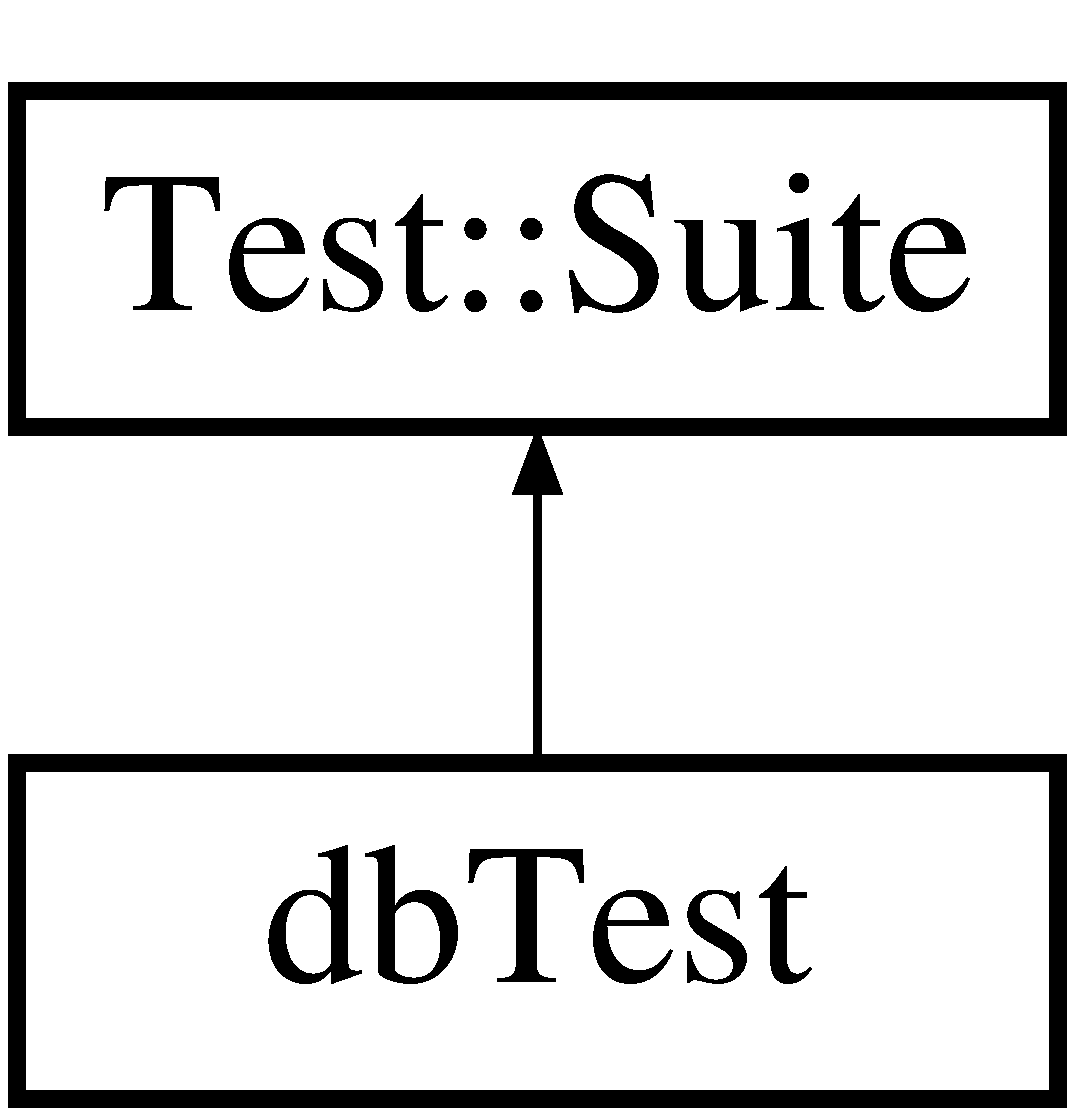
\includegraphics[height=2.000000cm]{class_test_1_1_suite}
\end{center}
\end{figure}
\subsection*{Public Member Functions}
\begin{DoxyCompactItemize}
\item 
\mbox{\hyperlink{class_test_1_1_suite_a8cb51a002cf4e675820f91fe03ec9117}{Suite}} ()
\item 
virtual \mbox{\hyperlink{class_test_1_1_suite_a2396d55bb8f9277e19dfdd4fd35421ec}{$\sim$\+Suite}} ()
\item 
void \mbox{\hyperlink{class_test_1_1_suite_a0237b63fc694ecb133d023cf2d6ab271}{add}} (std\+::auto\+\_\+ptr$<$ \mbox{\hyperlink{class_test_1_1_suite}{Suite}} $>$ suite)
\item 
bool \mbox{\hyperlink{class_test_1_1_suite_ad17746e218da79c537bc9d21e389f570}{run}} (\mbox{\hyperlink{class_test_1_1_output}{Output}} \&output, bool cont\+\_\+after\+\_\+fail=true)
\end{DoxyCompactItemize}
\subsection*{Protected Types}
\begin{DoxyCompactItemize}
\item 
typedef void(Suite\+::$\ast$ \mbox{\hyperlink{class_test_1_1_suite_a87c40a9c763fc3221bee0e70c431038f}{Func}}) ()
\end{DoxyCompactItemize}
\subsection*{Protected Member Functions}
\begin{DoxyCompactItemize}
\item 
bool \mbox{\hyperlink{class_test_1_1_suite_a3e2289069402291cdb100483a3247c16}{continue\+\_\+after\+\_\+failure}} () const
\item 
virtual void \mbox{\hyperlink{class_test_1_1_suite_aa022f93f2bc7c0ca4f8bf0bb94758226}{setup}} ()
\item 
virtual void \mbox{\hyperlink{class_test_1_1_suite_a2f2f180307180f8fdb0ca718a12047d0}{tear\+\_\+down}} ()
\item 
void \mbox{\hyperlink{class_test_1_1_suite_a11e542d1d45905b817b00c35660700b9}{register\+\_\+test}} (\mbox{\hyperlink{class_test_1_1_suite_a87c40a9c763fc3221bee0e70c431038f}{Func}} func, const std\+::string \&name)
\item 
void \mbox{\hyperlink{class_test_1_1_suite_a1851ad75aed6141a19a06eeeb0fe0d3c}{assertment}} (\mbox{\hyperlink{class_test_1_1_source}{Source}} s)
\end{DoxyCompactItemize}
\subsection*{Friends}
\begin{DoxyCompactItemize}
\item 
struct \mbox{\hyperlink{class_test_1_1_suite_a843435d7ee79d23ed13e6eec5c7ac6bb}{Do\+Run}}
\item 
struct \mbox{\hyperlink{class_test_1_1_suite_ab4730d33c1241aba407b71f8eafb7bcc}{Exec\+Tests}}
\item 
struct \mbox{\hyperlink{class_test_1_1_suite_a901d2d72cc93e087c94d99680f65fa8e}{Sub\+Suite\+Tests}}
\item 
struct \mbox{\hyperlink{class_test_1_1_suite_a5933776e455e5bd9ad1d4a8b1c591aa2}{Sub\+Suite\+Time}}
\end{DoxyCompactItemize}


\subsection{Detailed Description}
Unit testing suite. 

Base class for all suites. Derive from this class to create own test suites.

Test functions in derived classes are registered as tests using the \mbox{\hyperlink{cpptest-suite_8h_abe8c3e0a2cf3893ebc1c265264ed9cb8}{T\+E\+S\+T\+\_\+\+A\+D\+D(func)}}. Testing is started by \mbox{\hyperlink{class_test_1_1_suite_ad17746e218da79c537bc9d21e389f570}{run()}}. Note that suites may be embedded in other suites using \mbox{\hyperlink{class_test_1_1_suite_a0237b63fc694ecb133d023cf2d6ab271}{add()}}. 

Definition at line 52 of file cpptest-\/suite.\+h.



\subsection{Member Typedef Documentation}
\mbox{\Hypertarget{class_test_1_1_suite_a87c40a9c763fc3221bee0e70c431038f}\label{class_test_1_1_suite_a87c40a9c763fc3221bee0e70c431038f}} 
\index{Test\+::\+Suite@{Test\+::\+Suite}!Func@{Func}}
\index{Func@{Func}!Test\+::\+Suite@{Test\+::\+Suite}}
\subsubsection{\texorpdfstring{Func}{Func}}
{\footnotesize\ttfamily typedef void(Suite\+::$\ast$ Test\+::\+Suite\+::\+Func) ()\hspace{0.3cm}{\ttfamily [protected]}}

Pointer to a test function. 

Definition at line 65 of file cpptest-\/suite.\+h.



\subsection{Constructor \& Destructor Documentation}
\mbox{\Hypertarget{class_test_1_1_suite_a8cb51a002cf4e675820f91fe03ec9117}\label{class_test_1_1_suite_a8cb51a002cf4e675820f91fe03ec9117}} 
\index{Test\+::\+Suite@{Test\+::\+Suite}!Suite@{Suite}}
\index{Suite@{Suite}!Test\+::\+Suite@{Test\+::\+Suite}}
\subsubsection{\texorpdfstring{Suite()}{Suite()}}
{\footnotesize\ttfamily Test\+::\+Suite\+::\+Suite (\begin{DoxyParamCaption}{ }\end{DoxyParamCaption})}

\mbox{\Hypertarget{class_test_1_1_suite_a2396d55bb8f9277e19dfdd4fd35421ec}\label{class_test_1_1_suite_a2396d55bb8f9277e19dfdd4fd35421ec}} 
\index{Test\+::\+Suite@{Test\+::\+Suite}!````~Suite@{$\sim$\+Suite}}
\index{````~Suite@{$\sim$\+Suite}!Test\+::\+Suite@{Test\+::\+Suite}}
\subsubsection{\texorpdfstring{$\sim$\+Suite()}{~Suite()}}
{\footnotesize\ttfamily virtual Test\+::\+Suite\+::$\sim$\+Suite (\begin{DoxyParamCaption}{ }\end{DoxyParamCaption})\hspace{0.3cm}{\ttfamily [virtual]}}



\subsection{Member Function Documentation}
\mbox{\Hypertarget{class_test_1_1_suite_a0237b63fc694ecb133d023cf2d6ab271}\label{class_test_1_1_suite_a0237b63fc694ecb133d023cf2d6ab271}} 
\index{Test\+::\+Suite@{Test\+::\+Suite}!add@{add}}
\index{add@{add}!Test\+::\+Suite@{Test\+::\+Suite}}
\subsubsection{\texorpdfstring{add()}{add()}}
{\footnotesize\ttfamily void Test\+::\+Suite\+::add (\begin{DoxyParamCaption}\item[{std\+::auto\+\_\+ptr$<$ \mbox{\hyperlink{class_test_1_1_suite}{Suite}} $>$}]{suite }\end{DoxyParamCaption})}

\mbox{\Hypertarget{class_test_1_1_suite_a1851ad75aed6141a19a06eeeb0fe0d3c}\label{class_test_1_1_suite_a1851ad75aed6141a19a06eeeb0fe0d3c}} 
\index{Test\+::\+Suite@{Test\+::\+Suite}!assertment@{assertment}}
\index{assertment@{assertment}!Test\+::\+Suite@{Test\+::\+Suite}}
\subsubsection{\texorpdfstring{assertment()}{assertment()}}
{\footnotesize\ttfamily void Test\+::\+Suite\+::assertment (\begin{DoxyParamCaption}\item[{\mbox{\hyperlink{class_test_1_1_source}{Source}}}]{s }\end{DoxyParamCaption})\hspace{0.3cm}{\ttfamily [protected]}}

\mbox{\Hypertarget{class_test_1_1_suite_a3e2289069402291cdb100483a3247c16}\label{class_test_1_1_suite_a3e2289069402291cdb100483a3247c16}} 
\index{Test\+::\+Suite@{Test\+::\+Suite}!continue\+\_\+after\+\_\+failure@{continue\+\_\+after\+\_\+failure}}
\index{continue\+\_\+after\+\_\+failure@{continue\+\_\+after\+\_\+failure}!Test\+::\+Suite@{Test\+::\+Suite}}
\subsubsection{\texorpdfstring{continue\+\_\+after\+\_\+failure()}{continue\_after\_failure()}}
{\footnotesize\ttfamily bool Test\+::\+Suite\+::continue\+\_\+after\+\_\+failure (\begin{DoxyParamCaption}{ }\end{DoxyParamCaption}) const\hspace{0.3cm}{\ttfamily [inline]}, {\ttfamily [protected]}}



Definition at line 67 of file cpptest-\/suite.\+h.

\mbox{\Hypertarget{class_test_1_1_suite_a11e542d1d45905b817b00c35660700b9}\label{class_test_1_1_suite_a11e542d1d45905b817b00c35660700b9}} 
\index{Test\+::\+Suite@{Test\+::\+Suite}!register\+\_\+test@{register\+\_\+test}}
\index{register\+\_\+test@{register\+\_\+test}!Test\+::\+Suite@{Test\+::\+Suite}}
\subsubsection{\texorpdfstring{register\+\_\+test()}{register\_test()}}
{\footnotesize\ttfamily void Test\+::\+Suite\+::register\+\_\+test (\begin{DoxyParamCaption}\item[{\mbox{\hyperlink{class_test_1_1_suite_a87c40a9c763fc3221bee0e70c431038f}{Func}}}]{func,  }\item[{const std\+::string \&}]{name }\end{DoxyParamCaption})\hspace{0.3cm}{\ttfamily [protected]}}

\mbox{\Hypertarget{class_test_1_1_suite_ad17746e218da79c537bc9d21e389f570}\label{class_test_1_1_suite_ad17746e218da79c537bc9d21e389f570}} 
\index{Test\+::\+Suite@{Test\+::\+Suite}!run@{run}}
\index{run@{run}!Test\+::\+Suite@{Test\+::\+Suite}}
\subsubsection{\texorpdfstring{run()}{run()}}
{\footnotesize\ttfamily bool Test\+::\+Suite\+::run (\begin{DoxyParamCaption}\item[{\mbox{\hyperlink{class_test_1_1_output}{Output}} \&}]{output,  }\item[{bool}]{cont\+\_\+after\+\_\+fail = {\ttfamily true} }\end{DoxyParamCaption})}

\mbox{\Hypertarget{class_test_1_1_suite_aa022f93f2bc7c0ca4f8bf0bb94758226}\label{class_test_1_1_suite_aa022f93f2bc7c0ca4f8bf0bb94758226}} 
\index{Test\+::\+Suite@{Test\+::\+Suite}!setup@{setup}}
\index{setup@{setup}!Test\+::\+Suite@{Test\+::\+Suite}}
\subsubsection{\texorpdfstring{setup()}{setup()}}
{\footnotesize\ttfamily virtual void Test\+::\+Suite\+::setup (\begin{DoxyParamCaption}{ }\end{DoxyParamCaption})\hspace{0.3cm}{\ttfamily [inline]}, {\ttfamily [protected]}, {\ttfamily [virtual]}}



Reimplemented in \mbox{\hyperlink{classdb_test_aeefb6e8d64ee6e03da89cb5573d60b31}{db\+Test}}.



Definition at line 69 of file cpptest-\/suite.\+h.

\mbox{\Hypertarget{class_test_1_1_suite_a2f2f180307180f8fdb0ca718a12047d0}\label{class_test_1_1_suite_a2f2f180307180f8fdb0ca718a12047d0}} 
\index{Test\+::\+Suite@{Test\+::\+Suite}!tear\+\_\+down@{tear\+\_\+down}}
\index{tear\+\_\+down@{tear\+\_\+down}!Test\+::\+Suite@{Test\+::\+Suite}}
\subsubsection{\texorpdfstring{tear\+\_\+down()}{tear\_down()}}
{\footnotesize\ttfamily virtual void Test\+::\+Suite\+::tear\+\_\+down (\begin{DoxyParamCaption}{ }\end{DoxyParamCaption})\hspace{0.3cm}{\ttfamily [inline]}, {\ttfamily [protected]}, {\ttfamily [virtual]}}



Reimplemented in \mbox{\hyperlink{classdb_test_a1fa8de6f80f7578356b0f8feb8dcdd8f}{db\+Test}}.



Definition at line 70 of file cpptest-\/suite.\+h.



\subsection{Friends And Related Function Documentation}
\mbox{\Hypertarget{class_test_1_1_suite_a843435d7ee79d23ed13e6eec5c7ac6bb}\label{class_test_1_1_suite_a843435d7ee79d23ed13e6eec5c7ac6bb}} 
\index{Test\+::\+Suite@{Test\+::\+Suite}!Do\+Run@{Do\+Run}}
\index{Do\+Run@{Do\+Run}!Test\+::\+Suite@{Test\+::\+Suite}}
\subsubsection{\texorpdfstring{Do\+Run}{DoRun}}
{\footnotesize\ttfamily friend struct Do\+Run\hspace{0.3cm}{\ttfamily [friend]}}



Definition at line 80 of file cpptest-\/suite.\+h.

\mbox{\Hypertarget{class_test_1_1_suite_ab4730d33c1241aba407b71f8eafb7bcc}\label{class_test_1_1_suite_ab4730d33c1241aba407b71f8eafb7bcc}} 
\index{Test\+::\+Suite@{Test\+::\+Suite}!Exec\+Tests@{Exec\+Tests}}
\index{Exec\+Tests@{Exec\+Tests}!Test\+::\+Suite@{Test\+::\+Suite}}
\subsubsection{\texorpdfstring{Exec\+Tests}{ExecTests}}
{\footnotesize\ttfamily friend struct Exec\+Tests\hspace{0.3cm}{\ttfamily [friend]}}



Definition at line 83 of file cpptest-\/suite.\+h.

\mbox{\Hypertarget{class_test_1_1_suite_a901d2d72cc93e087c94d99680f65fa8e}\label{class_test_1_1_suite_a901d2d72cc93e087c94d99680f65fa8e}} 
\index{Test\+::\+Suite@{Test\+::\+Suite}!Sub\+Suite\+Tests@{Sub\+Suite\+Tests}}
\index{Sub\+Suite\+Tests@{Sub\+Suite\+Tests}!Test\+::\+Suite@{Test\+::\+Suite}}
\subsubsection{\texorpdfstring{Sub\+Suite\+Tests}{SubSuiteTests}}
{\footnotesize\ttfamily friend struct Sub\+Suite\+Tests\hspace{0.3cm}{\ttfamily [friend]}}



Definition at line 84 of file cpptest-\/suite.\+h.

\mbox{\Hypertarget{class_test_1_1_suite_a5933776e455e5bd9ad1d4a8b1c591aa2}\label{class_test_1_1_suite_a5933776e455e5bd9ad1d4a8b1c591aa2}} 
\index{Test\+::\+Suite@{Test\+::\+Suite}!Sub\+Suite\+Time@{Sub\+Suite\+Time}}
\index{Sub\+Suite\+Time@{Sub\+Suite\+Time}!Test\+::\+Suite@{Test\+::\+Suite}}
\subsubsection{\texorpdfstring{Sub\+Suite\+Time}{SubSuiteTime}}
{\footnotesize\ttfamily friend struct Sub\+Suite\+Time\hspace{0.3cm}{\ttfamily [friend]}}



Definition at line 85 of file cpptest-\/suite.\+h.



The documentation for this class was generated from the following file\+:\begin{DoxyCompactItemize}
\item 
\mbox{\hyperlink{cpptest-suite_8h}{cpptest-\/suite.\+h}}\end{DoxyCompactItemize}

\hypertarget{struct_test_1_1_collector_output_1_1_suite_info}{}\section{Test\+:\+:Collector\+Output\+:\+:Suite\+Info Struct Reference}
\label{struct_test_1_1_collector_output_1_1_suite_info}\index{Test\+::\+Collector\+Output\+::\+Suite\+Info@{Test\+::\+Collector\+Output\+::\+Suite\+Info}}


{\ttfamily \#include $<$cpptest-\/collectoroutput.\+h$>$}

\subsection*{Public Member Functions}
\begin{DoxyCompactItemize}
\item 
\mbox{\hyperlink{struct_test_1_1_collector_output_1_1_suite_info_a293cc820c5745fc786faf3b8e2ab9438}{Suite\+Info}} (const std\+::string \&name, int tests)
\end{DoxyCompactItemize}
\subsection*{Public Attributes}
\begin{DoxyCompactItemize}
\item 
std\+::string \mbox{\hyperlink{struct_test_1_1_collector_output_1_1_suite_info_a55bdc93b43037cba310bfd69441a3f15}{\+\_\+name}}
\item 
int \mbox{\hyperlink{struct_test_1_1_collector_output_1_1_suite_info_aad064ab88ce0e898be5b01ae98898e0f}{\+\_\+errors}}
\item 
\mbox{\hyperlink{class_test_1_1_collector_output_a54a7b7c9b6d181102bc8934190b06e86}{Tests}} \mbox{\hyperlink{struct_test_1_1_collector_output_1_1_suite_info_aeffb563714b2ba368e8c9cc92cb78091}{\+\_\+tests}}
\item 
\mbox{\hyperlink{class_test_1_1_time}{Time}} \mbox{\hyperlink{struct_test_1_1_collector_output_1_1_suite_info_a50173eba0cbf1c9e77bb029809a4580e}{\+\_\+time}}
\end{DoxyCompactItemize}


\subsection{Detailed Description}


Definition at line 79 of file cpptest-\/collectoroutput.\+h.



\subsection{Constructor \& Destructor Documentation}
\mbox{\Hypertarget{struct_test_1_1_collector_output_1_1_suite_info_a293cc820c5745fc786faf3b8e2ab9438}\label{struct_test_1_1_collector_output_1_1_suite_info_a293cc820c5745fc786faf3b8e2ab9438}} 
\index{Test\+::\+Collector\+Output\+::\+Suite\+Info@{Test\+::\+Collector\+Output\+::\+Suite\+Info}!Suite\+Info@{Suite\+Info}}
\index{Suite\+Info@{Suite\+Info}!Test\+::\+Collector\+Output\+::\+Suite\+Info@{Test\+::\+Collector\+Output\+::\+Suite\+Info}}
\subsubsection{\texorpdfstring{Suite\+Info()}{SuiteInfo()}}
{\footnotesize\ttfamily Test\+::\+Collector\+Output\+::\+Suite\+Info\+::\+Suite\+Info (\begin{DoxyParamCaption}\item[{const std\+::string \&}]{name,  }\item[{int}]{tests }\end{DoxyParamCaption})}



\subsection{Member Data Documentation}
\mbox{\Hypertarget{struct_test_1_1_collector_output_1_1_suite_info_aad064ab88ce0e898be5b01ae98898e0f}\label{struct_test_1_1_collector_output_1_1_suite_info_aad064ab88ce0e898be5b01ae98898e0f}} 
\index{Test\+::\+Collector\+Output\+::\+Suite\+Info@{Test\+::\+Collector\+Output\+::\+Suite\+Info}!\+\_\+errors@{\+\_\+errors}}
\index{\+\_\+errors@{\+\_\+errors}!Test\+::\+Collector\+Output\+::\+Suite\+Info@{Test\+::\+Collector\+Output\+::\+Suite\+Info}}
\subsubsection{\texorpdfstring{\+\_\+errors}{\_errors}}
{\footnotesize\ttfamily int Test\+::\+Collector\+Output\+::\+Suite\+Info\+::\+\_\+errors}



Definition at line 82 of file cpptest-\/collectoroutput.\+h.

\mbox{\Hypertarget{struct_test_1_1_collector_output_1_1_suite_info_a55bdc93b43037cba310bfd69441a3f15}\label{struct_test_1_1_collector_output_1_1_suite_info_a55bdc93b43037cba310bfd69441a3f15}} 
\index{Test\+::\+Collector\+Output\+::\+Suite\+Info@{Test\+::\+Collector\+Output\+::\+Suite\+Info}!\+\_\+name@{\+\_\+name}}
\index{\+\_\+name@{\+\_\+name}!Test\+::\+Collector\+Output\+::\+Suite\+Info@{Test\+::\+Collector\+Output\+::\+Suite\+Info}}
\subsubsection{\texorpdfstring{\+\_\+name}{\_name}}
{\footnotesize\ttfamily std\+::string Test\+::\+Collector\+Output\+::\+Suite\+Info\+::\+\_\+name}



Definition at line 81 of file cpptest-\/collectoroutput.\+h.

\mbox{\Hypertarget{struct_test_1_1_collector_output_1_1_suite_info_aeffb563714b2ba368e8c9cc92cb78091}\label{struct_test_1_1_collector_output_1_1_suite_info_aeffb563714b2ba368e8c9cc92cb78091}} 
\index{Test\+::\+Collector\+Output\+::\+Suite\+Info@{Test\+::\+Collector\+Output\+::\+Suite\+Info}!\+\_\+tests@{\+\_\+tests}}
\index{\+\_\+tests@{\+\_\+tests}!Test\+::\+Collector\+Output\+::\+Suite\+Info@{Test\+::\+Collector\+Output\+::\+Suite\+Info}}
\subsubsection{\texorpdfstring{\+\_\+tests}{\_tests}}
{\footnotesize\ttfamily \mbox{\hyperlink{class_test_1_1_collector_output_a54a7b7c9b6d181102bc8934190b06e86}{Tests}} Test\+::\+Collector\+Output\+::\+Suite\+Info\+::\+\_\+tests}



Definition at line 83 of file cpptest-\/collectoroutput.\+h.

\mbox{\Hypertarget{struct_test_1_1_collector_output_1_1_suite_info_a50173eba0cbf1c9e77bb029809a4580e}\label{struct_test_1_1_collector_output_1_1_suite_info_a50173eba0cbf1c9e77bb029809a4580e}} 
\index{Test\+::\+Collector\+Output\+::\+Suite\+Info@{Test\+::\+Collector\+Output\+::\+Suite\+Info}!\+\_\+time@{\+\_\+time}}
\index{\+\_\+time@{\+\_\+time}!Test\+::\+Collector\+Output\+::\+Suite\+Info@{Test\+::\+Collector\+Output\+::\+Suite\+Info}}
\subsubsection{\texorpdfstring{\+\_\+time}{\_time}}
{\footnotesize\ttfamily \mbox{\hyperlink{class_test_1_1_time}{Time}} Test\+::\+Collector\+Output\+::\+Suite\+Info\+::\+\_\+time}



Definition at line 84 of file cpptest-\/collectoroutput.\+h.



The documentation for this struct was generated from the following file\+:\begin{DoxyCompactItemize}
\item 
\mbox{\hyperlink{cpptest-collectoroutput_8h}{cpptest-\/collectoroutput.\+h}}\end{DoxyCompactItemize}

\hypertarget{struct_test_1_1_collector_output_1_1_test_info}{}\section{Test\+:\+:Collector\+Output\+:\+:Test\+Info Struct Reference}
\label{struct_test_1_1_collector_output_1_1_test_info}\index{Test\+::\+Collector\+Output\+::\+Test\+Info@{Test\+::\+Collector\+Output\+::\+Test\+Info}}


{\ttfamily \#include $<$cpptest-\/collectoroutput.\+h$>$}

\subsection*{Public Member Functions}
\begin{DoxyCompactItemize}
\item 
\mbox{\hyperlink{struct_test_1_1_collector_output_1_1_test_info_acfd49728d424c2824effe37beb85de87}{Test\+Info}} (const std\+::string name)
\end{DoxyCompactItemize}
\subsection*{Public Attributes}
\begin{DoxyCompactItemize}
\item 
std\+::string \mbox{\hyperlink{struct_test_1_1_collector_output_1_1_test_info_aa28d98e3ea65b4dda28fbb8c62817cf5}{\+\_\+name}}
\item 
\mbox{\hyperlink{class_test_1_1_time}{Time}} \mbox{\hyperlink{struct_test_1_1_collector_output_1_1_test_info_a59094663d5e7e2a7d896ce574ae6ef1b}{\+\_\+time}}
\item 
bool \mbox{\hyperlink{struct_test_1_1_collector_output_1_1_test_info_a99a6450e62566587a15c9ae9b7073ae7}{\+\_\+success}}\+: 1
\item 
\mbox{\hyperlink{class_test_1_1_collector_output_a1921f35e0da596bd75da5824afe872c9}{Sources}} \mbox{\hyperlink{struct_test_1_1_collector_output_1_1_test_info_a930eb868ea4e8fb30577967179c80d77}{\+\_\+sources}}
\end{DoxyCompactItemize}


\subsection{Detailed Description}


Definition at line 66 of file cpptest-\/collectoroutput.\+h.



\subsection{Constructor \& Destructor Documentation}
\mbox{\Hypertarget{struct_test_1_1_collector_output_1_1_test_info_acfd49728d424c2824effe37beb85de87}\label{struct_test_1_1_collector_output_1_1_test_info_acfd49728d424c2824effe37beb85de87}} 
\index{Test\+::\+Collector\+Output\+::\+Test\+Info@{Test\+::\+Collector\+Output\+::\+Test\+Info}!Test\+Info@{Test\+Info}}
\index{Test\+Info@{Test\+Info}!Test\+::\+Collector\+Output\+::\+Test\+Info@{Test\+::\+Collector\+Output\+::\+Test\+Info}}
\subsubsection{\texorpdfstring{Test\+Info()}{TestInfo()}}
{\footnotesize\ttfamily Test\+::\+Collector\+Output\+::\+Test\+Info\+::\+Test\+Info (\begin{DoxyParamCaption}\item[{const std\+::string}]{name }\end{DoxyParamCaption})\hspace{0.3cm}{\ttfamily [explicit]}}



\subsection{Member Data Documentation}
\mbox{\Hypertarget{struct_test_1_1_collector_output_1_1_test_info_aa28d98e3ea65b4dda28fbb8c62817cf5}\label{struct_test_1_1_collector_output_1_1_test_info_aa28d98e3ea65b4dda28fbb8c62817cf5}} 
\index{Test\+::\+Collector\+Output\+::\+Test\+Info@{Test\+::\+Collector\+Output\+::\+Test\+Info}!\+\_\+name@{\+\_\+name}}
\index{\+\_\+name@{\+\_\+name}!Test\+::\+Collector\+Output\+::\+Test\+Info@{Test\+::\+Collector\+Output\+::\+Test\+Info}}
\subsubsection{\texorpdfstring{\+\_\+name}{\_name}}
{\footnotesize\ttfamily std\+::string Test\+::\+Collector\+Output\+::\+Test\+Info\+::\+\_\+name}



Definition at line 68 of file cpptest-\/collectoroutput.\+h.

\mbox{\Hypertarget{struct_test_1_1_collector_output_1_1_test_info_a930eb868ea4e8fb30577967179c80d77}\label{struct_test_1_1_collector_output_1_1_test_info_a930eb868ea4e8fb30577967179c80d77}} 
\index{Test\+::\+Collector\+Output\+::\+Test\+Info@{Test\+::\+Collector\+Output\+::\+Test\+Info}!\+\_\+sources@{\+\_\+sources}}
\index{\+\_\+sources@{\+\_\+sources}!Test\+::\+Collector\+Output\+::\+Test\+Info@{Test\+::\+Collector\+Output\+::\+Test\+Info}}
\subsubsection{\texorpdfstring{\+\_\+sources}{\_sources}}
{\footnotesize\ttfamily \mbox{\hyperlink{class_test_1_1_collector_output_a1921f35e0da596bd75da5824afe872c9}{Sources}} Test\+::\+Collector\+Output\+::\+Test\+Info\+::\+\_\+sources}



Definition at line 72 of file cpptest-\/collectoroutput.\+h.

\mbox{\Hypertarget{struct_test_1_1_collector_output_1_1_test_info_a99a6450e62566587a15c9ae9b7073ae7}\label{struct_test_1_1_collector_output_1_1_test_info_a99a6450e62566587a15c9ae9b7073ae7}} 
\index{Test\+::\+Collector\+Output\+::\+Test\+Info@{Test\+::\+Collector\+Output\+::\+Test\+Info}!\+\_\+success@{\+\_\+success}}
\index{\+\_\+success@{\+\_\+success}!Test\+::\+Collector\+Output\+::\+Test\+Info@{Test\+::\+Collector\+Output\+::\+Test\+Info}}
\subsubsection{\texorpdfstring{\+\_\+success}{\_success}}
{\footnotesize\ttfamily bool Test\+::\+Collector\+Output\+::\+Test\+Info\+::\+\_\+success}



Definition at line 71 of file cpptest-\/collectoroutput.\+h.

\mbox{\Hypertarget{struct_test_1_1_collector_output_1_1_test_info_a59094663d5e7e2a7d896ce574ae6ef1b}\label{struct_test_1_1_collector_output_1_1_test_info_a59094663d5e7e2a7d896ce574ae6ef1b}} 
\index{Test\+::\+Collector\+Output\+::\+Test\+Info@{Test\+::\+Collector\+Output\+::\+Test\+Info}!\+\_\+time@{\+\_\+time}}
\index{\+\_\+time@{\+\_\+time}!Test\+::\+Collector\+Output\+::\+Test\+Info@{Test\+::\+Collector\+Output\+::\+Test\+Info}}
\subsubsection{\texorpdfstring{\+\_\+time}{\_time}}
{\footnotesize\ttfamily \mbox{\hyperlink{class_test_1_1_time}{Time}} Test\+::\+Collector\+Output\+::\+Test\+Info\+::\+\_\+time}



Definition at line 69 of file cpptest-\/collectoroutput.\+h.



The documentation for this struct was generated from the following file\+:\begin{DoxyCompactItemize}
\item 
\mbox{\hyperlink{cpptest-collectoroutput_8h}{cpptest-\/collectoroutput.\+h}}\end{DoxyCompactItemize}

\hypertarget{class_test_1_1_text_output}{}\section{Test\+:\+:Text\+Output Class Reference}
\label{class_test_1_1_text_output}\index{Test\+::\+Text\+Output@{Test\+::\+Text\+Output}}


Text output handler that outputs to the a stream.  




{\ttfamily \#include $<$cpptest-\/textoutput.\+h$>$}

Inheritance diagram for Test\+:\+:Text\+Output\+:\begin{figure}[H]
\begin{center}
\leavevmode
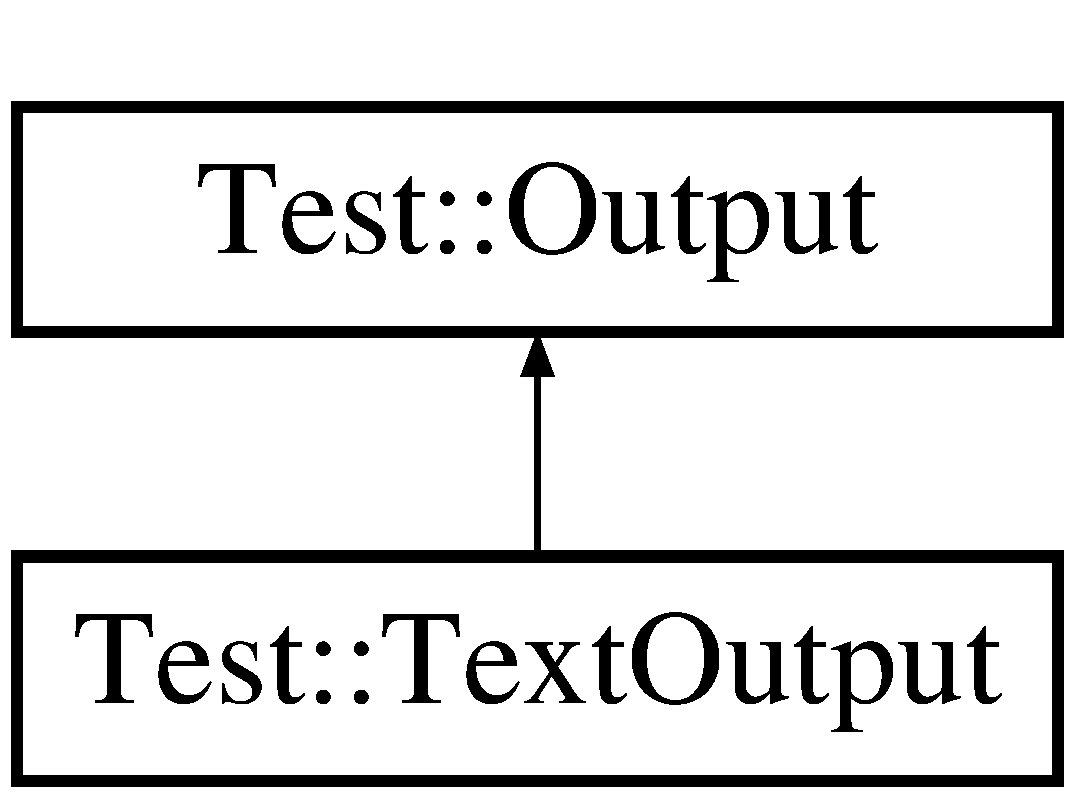
\includegraphics[height=2.000000cm]{class_test_1_1_text_output}
\end{center}
\end{figure}
\subsection*{Public Types}
\begin{DoxyCompactItemize}
\item 
enum \mbox{\hyperlink{class_test_1_1_text_output_ae7b22c9458e6c566996bf4517c73feb1}{Mode}} \{ \mbox{\hyperlink{class_test_1_1_text_output_ae7b22c9458e6c566996bf4517c73feb1ae63930203459836dfc6e0939f92a9fb2}{Terse}}, 
\mbox{\hyperlink{class_test_1_1_text_output_ae7b22c9458e6c566996bf4517c73feb1a85dd6e42f6261a23fd504201f5cc2792}{Verbose}}
 \}
\end{DoxyCompactItemize}
\subsection*{Public Member Functions}
\begin{DoxyCompactItemize}
\item 
\mbox{\hyperlink{class_test_1_1_text_output_ab9bdd9b2d9b362ca5fb148b766ecdd02}{Text\+Output}} (\mbox{\hyperlink{class_test_1_1_text_output_ae7b22c9458e6c566996bf4517c73feb1}{Mode}} mode, std\+::ostream \&stream=std\+::cout)
\item 
virtual void \mbox{\hyperlink{class_test_1_1_text_output_a9dcf13d9714a2774230386ef3215b701}{finished}} (int tests, const \mbox{\hyperlink{class_test_1_1_time}{Time}} \&time)
\item 
virtual void \mbox{\hyperlink{class_test_1_1_text_output_a0b6479918ee7f0501dfcdfcbc7c9d190}{suite\+\_\+start}} (int tests, const std\+::string \&name)
\item 
virtual void \mbox{\hyperlink{class_test_1_1_text_output_a84efd3536702a815325590cc8837dbb2}{suite\+\_\+end}} (int tests, const std\+::string \&name, const \mbox{\hyperlink{class_test_1_1_time}{Time}} \&time)
\item 
virtual void \mbox{\hyperlink{class_test_1_1_text_output_a0ff333537e85d680740c72dd46cd2e7e}{test\+\_\+end}} (const std\+::string \&name, bool ok, const \mbox{\hyperlink{class_test_1_1_time}{Time}} \&time)
\item 
virtual void \mbox{\hyperlink{class_test_1_1_text_output_a8110f86aa00f783fc5a91ec2f59a7998}{assertment}} (const \mbox{\hyperlink{class_test_1_1_source}{Source}} \&s)
\end{DoxyCompactItemize}
\subsection*{Additional Inherited Members}


\subsection{Detailed Description}
Text output handler that outputs to the a stream. 

Test suite output handler that writes its information as text to a a stream. It it possible to select between two different operational modes that controls the detail level, see Mode. 

Definition at line 46 of file cpptest-\/textoutput.\+h.



\subsection{Member Enumeration Documentation}
\mbox{\Hypertarget{class_test_1_1_text_output_ae7b22c9458e6c566996bf4517c73feb1}\label{class_test_1_1_text_output_ae7b22c9458e6c566996bf4517c73feb1}} 
\index{Test\+::\+Text\+Output@{Test\+::\+Text\+Output}!Mode@{Mode}}
\index{Mode@{Mode}!Test\+::\+Text\+Output@{Test\+::\+Text\+Output}}
\subsubsection{\texorpdfstring{Mode}{Mode}}
{\footnotesize\ttfamily enum \mbox{\hyperlink{class_test_1_1_text_output_ae7b22c9458e6c566996bf4517c73feb1}{Test\+::\+Text\+Output\+::\+Mode}}}

\mbox{\hyperlink{class_test_1_1_output}{Output}} mode. \begin{DoxyEnumFields}{Enumerator}
\raisebox{\heightof{T}}[0pt][0pt]{\index{Terse@{Terse}!Test\+::\+Text\+Output@{Test\+::\+Text\+Output}}\index{Test\+::\+Text\+Output@{Test\+::\+Text\+Output}!Terse@{Terse}}}\mbox{\Hypertarget{class_test_1_1_text_output_ae7b22c9458e6c566996bf4517c73feb1ae63930203459836dfc6e0939f92a9fb2}\label{class_test_1_1_text_output_ae7b22c9458e6c566996bf4517c73feb1ae63930203459836dfc6e0939f92a9fb2}} 
Terse&Terse output mode, which only shows the number of correct tests. \\
\hline

\raisebox{\heightof{T}}[0pt][0pt]{\index{Verbose@{Verbose}!Test\+::\+Text\+Output@{Test\+::\+Text\+Output}}\index{Test\+::\+Text\+Output@{Test\+::\+Text\+Output}!Verbose@{Verbose}}}\mbox{\Hypertarget{class_test_1_1_text_output_ae7b22c9458e6c566996bf4517c73feb1a85dd6e42f6261a23fd504201f5cc2792}\label{class_test_1_1_text_output_ae7b22c9458e6c566996bf4517c73feb1a85dd6e42f6261a23fd504201f5cc2792}} 
Verbose&Verbose output mode, which also shows extended assert information for each test that failed. \\
\hline

\end{DoxyEnumFields}


Definition at line 51 of file cpptest-\/textoutput.\+h.



\subsection{Constructor \& Destructor Documentation}
\mbox{\Hypertarget{class_test_1_1_text_output_ab9bdd9b2d9b362ca5fb148b766ecdd02}\label{class_test_1_1_text_output_ab9bdd9b2d9b362ca5fb148b766ecdd02}} 
\index{Test\+::\+Text\+Output@{Test\+::\+Text\+Output}!Text\+Output@{Text\+Output}}
\index{Text\+Output@{Text\+Output}!Test\+::\+Text\+Output@{Test\+::\+Text\+Output}}
\subsubsection{\texorpdfstring{Text\+Output()}{TextOutput()}}
{\footnotesize\ttfamily Test\+::\+Text\+Output\+::\+Text\+Output (\begin{DoxyParamCaption}\item[{\mbox{\hyperlink{class_test_1_1_text_output_ae7b22c9458e6c566996bf4517c73feb1}{Mode}}}]{mode,  }\item[{std\+::ostream \&}]{stream = {\ttfamily std\+:\+:cout} }\end{DoxyParamCaption})}



\subsection{Member Function Documentation}
\mbox{\Hypertarget{class_test_1_1_text_output_a8110f86aa00f783fc5a91ec2f59a7998}\label{class_test_1_1_text_output_a8110f86aa00f783fc5a91ec2f59a7998}} 
\index{Test\+::\+Text\+Output@{Test\+::\+Text\+Output}!assertment@{assertment}}
\index{assertment@{assertment}!Test\+::\+Text\+Output@{Test\+::\+Text\+Output}}
\subsubsection{\texorpdfstring{assertment()}{assertment()}}
{\footnotesize\ttfamily virtual void Test\+::\+Text\+Output\+::assertment (\begin{DoxyParamCaption}\item[{const \mbox{\hyperlink{class_test_1_1_source}{Source}} \&}]{s }\end{DoxyParamCaption})\hspace{0.3cm}{\ttfamily [virtual]}}

Called when an assertment is issued.


\begin{DoxyParams}{Parameters}
{\em s} & Assert point information. \\
\hline
\end{DoxyParams}


Reimplemented from \mbox{\hyperlink{class_test_1_1_output_a48c31f0baa7627d81939be840c9a7f65}{Test\+::\+Output}}.

\mbox{\Hypertarget{class_test_1_1_text_output_a9dcf13d9714a2774230386ef3215b701}\label{class_test_1_1_text_output_a9dcf13d9714a2774230386ef3215b701}} 
\index{Test\+::\+Text\+Output@{Test\+::\+Text\+Output}!finished@{finished}}
\index{finished@{finished}!Test\+::\+Text\+Output@{Test\+::\+Text\+Output}}
\subsubsection{\texorpdfstring{finished()}{finished()}}
{\footnotesize\ttfamily virtual void Test\+::\+Text\+Output\+::finished (\begin{DoxyParamCaption}\item[{int}]{tests,  }\item[{const \mbox{\hyperlink{class_test_1_1_time}{Time}} \&}]{time }\end{DoxyParamCaption})\hspace{0.3cm}{\ttfamily [virtual]}}

Called when testing is finished.


\begin{DoxyParams}{Parameters}
{\em tests} & Total number of tests in all suites. \\
\hline
{\em time} & Total elapsed time for all tests. \\
\hline
\end{DoxyParams}


Reimplemented from \mbox{\hyperlink{class_test_1_1_output_aeff8af8326a8c54a38199f76837f860a}{Test\+::\+Output}}.

\mbox{\Hypertarget{class_test_1_1_text_output_a84efd3536702a815325590cc8837dbb2}\label{class_test_1_1_text_output_a84efd3536702a815325590cc8837dbb2}} 
\index{Test\+::\+Text\+Output@{Test\+::\+Text\+Output}!suite\+\_\+end@{suite\+\_\+end}}
\index{suite\+\_\+end@{suite\+\_\+end}!Test\+::\+Text\+Output@{Test\+::\+Text\+Output}}
\subsubsection{\texorpdfstring{suite\+\_\+end()}{suite\_end()}}
{\footnotesize\ttfamily virtual void Test\+::\+Text\+Output\+::suite\+\_\+end (\begin{DoxyParamCaption}\item[{int}]{tests,  }\item[{const std\+::string \&}]{name,  }\item[{const \mbox{\hyperlink{class_test_1_1_time}{Time}} \&}]{time }\end{DoxyParamCaption})\hspace{0.3cm}{\ttfamily [virtual]}}

Called when a suite is finished.


\begin{DoxyParams}{Parameters}
{\em tests} & Number of tests in this suite. \\
\hline
{\em name} & Name of the suite. \\
\hline
{\em time} & Total elapsed time for all tests in this suite. \\
\hline
\end{DoxyParams}


Reimplemented from \mbox{\hyperlink{class_test_1_1_output_a6dbf4c0adb2bd4a7364c629179f788a6}{Test\+::\+Output}}.

\mbox{\Hypertarget{class_test_1_1_text_output_a0b6479918ee7f0501dfcdfcbc7c9d190}\label{class_test_1_1_text_output_a0b6479918ee7f0501dfcdfcbc7c9d190}} 
\index{Test\+::\+Text\+Output@{Test\+::\+Text\+Output}!suite\+\_\+start@{suite\+\_\+start}}
\index{suite\+\_\+start@{suite\+\_\+start}!Test\+::\+Text\+Output@{Test\+::\+Text\+Output}}
\subsubsection{\texorpdfstring{suite\+\_\+start()}{suite\_start()}}
{\footnotesize\ttfamily virtual void Test\+::\+Text\+Output\+::suite\+\_\+start (\begin{DoxyParamCaption}\item[{int}]{tests,  }\item[{const std\+::string \&}]{name }\end{DoxyParamCaption})\hspace{0.3cm}{\ttfamily [virtual]}}

Called when a suite is entered.


\begin{DoxyParams}{Parameters}
{\em tests} & Number of tests in this suite. \\
\hline
{\em name} & Name of the suite. \\
\hline
\end{DoxyParams}


Reimplemented from \mbox{\hyperlink{class_test_1_1_output_a7022c32c5a1577b10b93d3942746f17d}{Test\+::\+Output}}.

\mbox{\Hypertarget{class_test_1_1_text_output_a0ff333537e85d680740c72dd46cd2e7e}\label{class_test_1_1_text_output_a0ff333537e85d680740c72dd46cd2e7e}} 
\index{Test\+::\+Text\+Output@{Test\+::\+Text\+Output}!test\+\_\+end@{test\+\_\+end}}
\index{test\+\_\+end@{test\+\_\+end}!Test\+::\+Text\+Output@{Test\+::\+Text\+Output}}
\subsubsection{\texorpdfstring{test\+\_\+end()}{test\_end()}}
{\footnotesize\ttfamily virtual void Test\+::\+Text\+Output\+::test\+\_\+end (\begin{DoxyParamCaption}\item[{const std\+::string \&}]{name,  }\item[{bool}]{ok,  }\item[{const \mbox{\hyperlink{class_test_1_1_time}{Time}} \&}]{time }\end{DoxyParamCaption})\hspace{0.3cm}{\ttfamily [virtual]}}

Called when a test if finished, regardless if an assertment was issued.


\begin{DoxyParams}{Parameters}
{\em name} & Name of the test function. \\
\hline
{\em ok} & True if the test was successful; false otherwise. \\
\hline
{\em time} & Execution time. \\
\hline
\end{DoxyParams}


Reimplemented from \mbox{\hyperlink{class_test_1_1_output_a3796943e3b56373492c957212a21454e}{Test\+::\+Output}}.



The documentation for this class was generated from the following file\+:\begin{DoxyCompactItemize}
\item 
\mbox{\hyperlink{cpptest-textoutput_8h}{cpptest-\/textoutput.\+h}}\end{DoxyCompactItemize}

\hypertarget{class_test_1_1_time}{}\section{Test\+:\+:Time Class Reference}
\label{class_test_1_1_time}\index{Test\+::\+Time@{Test\+::\+Time}}


Time representation.  




{\ttfamily \#include $<$cpptest-\/time.\+h$>$}

\subsection*{Public Member Functions}
\begin{DoxyCompactItemize}
\item 
\mbox{\hyperlink{class_test_1_1_time_ae5c1089d2eb013c5b908ea95d924b733}{Time}} ()
\item 
\mbox{\hyperlink{class_test_1_1_time_afdc9c0556b8d71ecd8d621c2512154a5}{Time}} (unsigned int sec, unsigned int usec)
\item 
unsigned int \mbox{\hyperlink{class_test_1_1_time_a75a6145c4502fc9c1a3f5171c6536b07}{seconds}} () const
\item 
unsigned int \mbox{\hyperlink{class_test_1_1_time_a49a77156512509bea4bb49b614a5ecc8}{microseconds}} () const
\end{DoxyCompactItemize}
\subsection*{Static Public Member Functions}
\begin{DoxyCompactItemize}
\item 
static \mbox{\hyperlink{class_test_1_1_time}{Time}} \mbox{\hyperlink{class_test_1_1_time_a83422a11d27c17a7a4bc52ab14fdb9a3}{current}} ()
\end{DoxyCompactItemize}
\subsection*{Friends}
\begin{DoxyCompactItemize}
\item 
\mbox{\hyperlink{class_test_1_1_time}{Time}} \mbox{\hyperlink{class_test_1_1_time_ae2e555aa5b5c51e44b576d8baf48a2cd}{operator+}} (const \mbox{\hyperlink{class_test_1_1_time}{Time}} \&t1, const \mbox{\hyperlink{class_test_1_1_time}{Time}} \&t2)
\item 
\mbox{\hyperlink{class_test_1_1_time}{Time}} \mbox{\hyperlink{class_test_1_1_time_a09225563b0b317910b26c550ba74de64}{operator-\/}} (const \mbox{\hyperlink{class_test_1_1_time}{Time}} \&t1, const \mbox{\hyperlink{class_test_1_1_time}{Time}} \&t2)
\item 
std\+::ostream \& \mbox{\hyperlink{class_test_1_1_time_a0287b008277738b9882ed96467e8b4f8}{operator$<$$<$}} (std\+::ostream \&os, const \mbox{\hyperlink{class_test_1_1_time}{Time}} \&t)
\end{DoxyCompactItemize}


\subsection{Detailed Description}
Time representation. 

Encapsulates a time value with microsecond resolution. It is possible to retrieve the current time, add and subtract time values, and output the time to an output stream. 

Definition at line 43 of file cpptest-\/time.\+h.



\subsection{Constructor \& Destructor Documentation}
\mbox{\Hypertarget{class_test_1_1_time_ae5c1089d2eb013c5b908ea95d924b733}\label{class_test_1_1_time_ae5c1089d2eb013c5b908ea95d924b733}} 
\index{Test\+::\+Time@{Test\+::\+Time}!Time@{Time}}
\index{Time@{Time}!Test\+::\+Time@{Test\+::\+Time}}
\subsubsection{\texorpdfstring{Time()}{Time()}\hspace{0.1cm}{\footnotesize\ttfamily [1/2]}}
{\footnotesize\ttfamily Test\+::\+Time\+::\+Time (\begin{DoxyParamCaption}{ }\end{DoxyParamCaption})}

\mbox{\Hypertarget{class_test_1_1_time_afdc9c0556b8d71ecd8d621c2512154a5}\label{class_test_1_1_time_afdc9c0556b8d71ecd8d621c2512154a5}} 
\index{Test\+::\+Time@{Test\+::\+Time}!Time@{Time}}
\index{Time@{Time}!Test\+::\+Time@{Test\+::\+Time}}
\subsubsection{\texorpdfstring{Time()}{Time()}\hspace{0.1cm}{\footnotesize\ttfamily [2/2]}}
{\footnotesize\ttfamily Test\+::\+Time\+::\+Time (\begin{DoxyParamCaption}\item[{unsigned int}]{sec,  }\item[{unsigned int}]{usec }\end{DoxyParamCaption})}



\subsection{Member Function Documentation}
\mbox{\Hypertarget{class_test_1_1_time_a83422a11d27c17a7a4bc52ab14fdb9a3}\label{class_test_1_1_time_a83422a11d27c17a7a4bc52ab14fdb9a3}} 
\index{Test\+::\+Time@{Test\+::\+Time}!current@{current}}
\index{current@{current}!Test\+::\+Time@{Test\+::\+Time}}
\subsubsection{\texorpdfstring{current()}{current()}}
{\footnotesize\ttfamily static \mbox{\hyperlink{class_test_1_1_time}{Time}} Test\+::\+Time\+::current (\begin{DoxyParamCaption}{ }\end{DoxyParamCaption})\hspace{0.3cm}{\ttfamily [static]}}

\mbox{\Hypertarget{class_test_1_1_time_a49a77156512509bea4bb49b614a5ecc8}\label{class_test_1_1_time_a49a77156512509bea4bb49b614a5ecc8}} 
\index{Test\+::\+Time@{Test\+::\+Time}!microseconds@{microseconds}}
\index{microseconds@{microseconds}!Test\+::\+Time@{Test\+::\+Time}}
\subsubsection{\texorpdfstring{microseconds()}{microseconds()}}
{\footnotesize\ttfamily unsigned int Test\+::\+Time\+::microseconds (\begin{DoxyParamCaption}{ }\end{DoxyParamCaption}) const}

\mbox{\Hypertarget{class_test_1_1_time_a75a6145c4502fc9c1a3f5171c6536b07}\label{class_test_1_1_time_a75a6145c4502fc9c1a3f5171c6536b07}} 
\index{Test\+::\+Time@{Test\+::\+Time}!seconds@{seconds}}
\index{seconds@{seconds}!Test\+::\+Time@{Test\+::\+Time}}
\subsubsection{\texorpdfstring{seconds()}{seconds()}}
{\footnotesize\ttfamily unsigned int Test\+::\+Time\+::seconds (\begin{DoxyParamCaption}{ }\end{DoxyParamCaption}) const}



\subsection{Friends And Related Function Documentation}
\mbox{\Hypertarget{class_test_1_1_time_ae2e555aa5b5c51e44b576d8baf48a2cd}\label{class_test_1_1_time_ae2e555aa5b5c51e44b576d8baf48a2cd}} 
\index{Test\+::\+Time@{Test\+::\+Time}!operator+@{operator+}}
\index{operator+@{operator+}!Test\+::\+Time@{Test\+::\+Time}}
\subsubsection{\texorpdfstring{operator+}{operator+}}
{\footnotesize\ttfamily \mbox{\hyperlink{class_test_1_1_time}{Time}} operator+ (\begin{DoxyParamCaption}\item[{const \mbox{\hyperlink{class_test_1_1_time}{Time}} \&}]{t1,  }\item[{const \mbox{\hyperlink{class_test_1_1_time}{Time}} \&}]{t2 }\end{DoxyParamCaption})\hspace{0.3cm}{\ttfamily [friend]}}

\mbox{\Hypertarget{class_test_1_1_time_a09225563b0b317910b26c550ba74de64}\label{class_test_1_1_time_a09225563b0b317910b26c550ba74de64}} 
\index{Test\+::\+Time@{Test\+::\+Time}!operator-\/@{operator-\/}}
\index{operator-\/@{operator-\/}!Test\+::\+Time@{Test\+::\+Time}}
\subsubsection{\texorpdfstring{operator-\/}{operator-}}
{\footnotesize\ttfamily \mbox{\hyperlink{class_test_1_1_time}{Time}} operator-\/ (\begin{DoxyParamCaption}\item[{const \mbox{\hyperlink{class_test_1_1_time}{Time}} \&}]{t1,  }\item[{const \mbox{\hyperlink{class_test_1_1_time}{Time}} \&}]{t2 }\end{DoxyParamCaption})\hspace{0.3cm}{\ttfamily [friend]}}

\mbox{\Hypertarget{class_test_1_1_time_a0287b008277738b9882ed96467e8b4f8}\label{class_test_1_1_time_a0287b008277738b9882ed96467e8b4f8}} 
\index{Test\+::\+Time@{Test\+::\+Time}!operator$<$$<$@{operator$<$$<$}}
\index{operator$<$$<$@{operator$<$$<$}!Test\+::\+Time@{Test\+::\+Time}}
\subsubsection{\texorpdfstring{operator$<$$<$}{operator<<}}
{\footnotesize\ttfamily std\+::ostream\& operator$<$$<$ (\begin{DoxyParamCaption}\item[{std\+::ostream \&}]{os,  }\item[{const \mbox{\hyperlink{class_test_1_1_time}{Time}} \&}]{t }\end{DoxyParamCaption})\hspace{0.3cm}{\ttfamily [friend]}}



The documentation for this class was generated from the following file\+:\begin{DoxyCompactItemize}
\item 
\mbox{\hyperlink{cpptest-time_8h}{cpptest-\/time.\+h}}\end{DoxyCompactItemize}

\chapter{File Documentation}
\hypertarget{_console_application1_8cpp}{}\section{Console\+Application1.\+cpp File Reference}
\label{_console_application1_8cpp}\index{Console\+Application1.\+cpp@{Console\+Application1.\+cpp}}
{\ttfamily \#include \char`\"{}stdafx.\+h\char`\"{}}\newline
{\ttfamily \#include $<$sstream$>$}\newline
{\ttfamily \#include \char`\"{}Record\+Processor.\+h\char`\"{}}\newline
{\ttfamily \#include \char`\"{}cpptest.\+h\char`\"{}}\newline
\subsection*{Classes}
\begin{DoxyCompactItemize}
\item 
class \mbox{\hyperlink{classdb_test}{db\+Test}}
\end{DoxyCompactItemize}
\subsection*{Functions}
\begin{DoxyCompactItemize}
\item 
int \mbox{\hyperlink{_console_application1_8cpp_ae66f6b31b5ad750f1fe042a706a4e3d4}{main}} ()
\end{DoxyCompactItemize}


\subsection{Function Documentation}
\mbox{\Hypertarget{_console_application1_8cpp_ae66f6b31b5ad750f1fe042a706a4e3d4}\label{_console_application1_8cpp_ae66f6b31b5ad750f1fe042a706a4e3d4}} 
\index{Console\+Application1.\+cpp@{Console\+Application1.\+cpp}!main@{main}}
\index{main@{main}!Console\+Application1.\+cpp@{Console\+Application1.\+cpp}}
\subsubsection{\texorpdfstring{main()}{main()}}
{\footnotesize\ttfamily int main (\begin{DoxyParamCaption}{ }\end{DoxyParamCaption})}



Definition at line 146 of file Console\+Application1.\+cpp.


\hypertarget{cpptest-assert_8h}{}\section{cpptest-\/assert.h File Reference}
\label{cpptest-assert_8h}\index{cpptest-\/assert.\+h@{cpptest-\/assert.\+h}}
{\ttfamily \#include $<$sstream$>$}\newline
\subsection*{Macros}
\begin{DoxyCompactItemize}
\item 
\#define \mbox{\hyperlink{cpptest-assert_8h_a947ab44cc42369eb7cfe33f8a1e38e4b}{T\+E\+S\+T\+\_\+\+F\+A\+IL}}(msg)
\item 
\#define \mbox{\hyperlink{cpptest-assert_8h_a29a763f14098f5574ae5c68291dc6ddd}{T\+E\+S\+T\+\_\+\+A\+S\+S\+E\+RT}}(expr)
\item 
\#define \mbox{\hyperlink{cpptest-assert_8h_ac612ede938734f9c8d898e05818882fb}{T\+E\+S\+T\+\_\+\+A\+S\+S\+E\+R\+T\+\_\+\+M\+SG}}(expr,  msg)
\item 
\#define \mbox{\hyperlink{cpptest-assert_8h_ae281f4d973e657b11691a97551f17dd1}{T\+E\+S\+T\+\_\+\+A\+S\+S\+E\+R\+T\+\_\+\+E\+Q\+U\+A\+LS}}(expected,  got)
\item 
\#define \mbox{\hyperlink{cpptest-assert_8h_aa506d98e8a5fc575df0361906f7deef8}{T\+E\+S\+T\+\_\+\+A\+S\+S\+E\+R\+T\+\_\+\+E\+Q\+U\+A\+L\+S\+\_\+\+O\+BJ}}(expected,  got)
\item 
\#define \mbox{\hyperlink{cpptest-assert_8h_ab8e9ce729f96abe74b76d98f9568a59c}{T\+E\+S\+T\+\_\+\+A\+S\+S\+E\+R\+T\+\_\+\+E\+Q\+U\+A\+L\+S\+\_\+\+M\+SG}}(expected,  got,  msg)
\item 
\#define \mbox{\hyperlink{cpptest-assert_8h_a9583b1709f4b9dfb3ff2849bfec5c885}{T\+E\+S\+T\+\_\+\+A\+S\+S\+E\+R\+T\+\_\+\+D\+E\+L\+TA}}(a,  b,  delta)
\item 
\#define \mbox{\hyperlink{cpptest-assert_8h_afcd749452840bfde9be575ef22fcede0}{T\+E\+S\+T\+\_\+\+A\+S\+S\+E\+R\+T\+\_\+\+D\+E\+L\+T\+A\+\_\+\+M\+SG}}(a,  b,  delta,  msg)
\item 
\#define \mbox{\hyperlink{cpptest-assert_8h_a5174c5f93519d5726c8993b2f36d6ceb}{T\+E\+S\+T\+\_\+\+T\+H\+R\+O\+WS}}(expr,  x)
\item 
\#define \mbox{\hyperlink{cpptest-assert_8h_a1ce6abe9e9134ce993840a648673e0f2}{T\+E\+S\+T\+\_\+\+T\+H\+R\+O\+W\+S\+\_\+\+M\+SG}}(expr,  x,  msg)
\item 
\#define \mbox{\hyperlink{cpptest-assert_8h_a895af88056cd626a010136ac07b81d37}{T\+E\+S\+T\+\_\+\+T\+H\+R\+O\+W\+S\+\_\+\+A\+N\+Y\+T\+H\+I\+NG}}(expr)
\item 
\#define \mbox{\hyperlink{cpptest-assert_8h_a052597a8fd7dbc40ba350c735c4517c5}{T\+E\+S\+T\+\_\+\+T\+H\+R\+O\+W\+S\+\_\+\+A\+N\+Y\+T\+H\+I\+N\+G\+\_\+\+M\+SG}}(expr,  msg)
\item 
\#define \mbox{\hyperlink{cpptest-assert_8h_a885a5f6b6decac47414b4cc1a0a66425}{T\+E\+S\+T\+\_\+\+T\+H\+R\+O\+W\+S\+\_\+\+N\+O\+T\+H\+I\+NG}}(expr)
\item 
\#define \mbox{\hyperlink{cpptest-assert_8h_a758a47b613522a3d597c513786191ff9}{T\+E\+S\+T\+\_\+\+T\+H\+R\+O\+W\+S\+\_\+\+N\+O\+T\+H\+I\+N\+G\+\_\+\+M\+SG}}(expr,  msg)
\end{DoxyCompactItemize}


\subsection{Macro Definition Documentation}
\mbox{\Hypertarget{cpptest-assert_8h_a29a763f14098f5574ae5c68291dc6ddd}\label{cpptest-assert_8h_a29a763f14098f5574ae5c68291dc6ddd}} 
\index{cpptest-\/assert.\+h@{cpptest-\/assert.\+h}!T\+E\+S\+T\+\_\+\+A\+S\+S\+E\+RT@{T\+E\+S\+T\+\_\+\+A\+S\+S\+E\+RT}}
\index{T\+E\+S\+T\+\_\+\+A\+S\+S\+E\+RT@{T\+E\+S\+T\+\_\+\+A\+S\+S\+E\+RT}!cpptest-\/assert.\+h@{cpptest-\/assert.\+h}}
\subsubsection{\texorpdfstring{T\+E\+S\+T\+\_\+\+A\+S\+S\+E\+RT}{TEST\_ASSERT}}
{\footnotesize\ttfamily \#define T\+E\+S\+T\+\_\+\+A\+S\+S\+E\+RT(\begin{DoxyParamCaption}\item[{}]{expr }\end{DoxyParamCaption})}

{\bfseries Value\+:}
\begin{DoxyCode}
\{                                                               \(\backslash\)
        if (!(expr))                                                \(\backslash\)
        \{                                                           \(\backslash\)
            assertment(::\mbox{\hyperlink{class_test_1_1_source}{Test::Source}}(\_\_FILE\_\_, \_\_LINE\_\_, #expr));  \(\backslash\)
            if (!continue\_after\_failure()) return;                  \(\backslash\)
        \}                                                           \(\backslash\)
    \}
\end{DoxyCode}
Verify an expression and issues an assertment if it fails.

Used in conjunction with \mbox{\hyperlink{class_test_1_1_suite}{Test\+::\+Suite}}.


\begin{DoxyParams}{Parameters}
{\em expr} & Expression to test.\\
\hline
\end{DoxyParams}
\begin{DoxySeeAlso}{See also}
\mbox{\hyperlink{cpptest-assert_8h_ac612ede938734f9c8d898e05818882fb}{T\+E\+S\+T\+\_\+\+A\+S\+S\+E\+R\+T\+\_\+\+M\+S\+G(expr, msg)}}
\end{DoxySeeAlso}
\begin{DoxyParagraph}{Example\+:}

\begin{DoxyCode}
\textcolor{keywordtype}{void} MySuite::test()
\{
    \textcolor{keywordtype}{int} i;

    \textcolor{comment}{// ...}

    \mbox{\hyperlink{cpptest-assert_8h_a29a763f14098f5574ae5c68291dc6ddd}{TEST\_ASSERT}}(i == 13)
\}
\end{DoxyCode}

\end{DoxyParagraph}
For a description of all asserts, see \mbox{\hyperlink{asserts}{Available asserts}}. 

Definition at line 87 of file cpptest-\/assert.\+h.

\mbox{\Hypertarget{cpptest-assert_8h_a9583b1709f4b9dfb3ff2849bfec5c885}\label{cpptest-assert_8h_a9583b1709f4b9dfb3ff2849bfec5c885}} 
\index{cpptest-\/assert.\+h@{cpptest-\/assert.\+h}!T\+E\+S\+T\+\_\+\+A\+S\+S\+E\+R\+T\+\_\+\+D\+E\+L\+TA@{T\+E\+S\+T\+\_\+\+A\+S\+S\+E\+R\+T\+\_\+\+D\+E\+L\+TA}}
\index{T\+E\+S\+T\+\_\+\+A\+S\+S\+E\+R\+T\+\_\+\+D\+E\+L\+TA@{T\+E\+S\+T\+\_\+\+A\+S\+S\+E\+R\+T\+\_\+\+D\+E\+L\+TA}!cpptest-\/assert.\+h@{cpptest-\/assert.\+h}}
\subsubsection{\texorpdfstring{T\+E\+S\+T\+\_\+\+A\+S\+S\+E\+R\+T\+\_\+\+D\+E\+L\+TA}{TEST\_ASSERT\_DELTA}}
{\footnotesize\ttfamily \#define T\+E\+S\+T\+\_\+\+A\+S\+S\+E\+R\+T\+\_\+\+D\+E\+L\+TA(\begin{DoxyParamCaption}\item[{}]{a,  }\item[{}]{b,  }\item[{}]{delta }\end{DoxyParamCaption})}

{\bfseries Value\+:}
\begin{DoxyCode}
\{                                                               \(\backslash\)
        if (((b) < (a) - (delta)) || ((b) > (a) + (delta)))         \(\backslash\)
        \{                                                           \(\backslash\)
            assertment(::\mbox{\hyperlink{class_test_1_1_source}{Test::Source}}(\_\_FILE\_\_, \_\_LINE\_\_,           \(\backslash\)
                       \textcolor{stringliteral}{"delta("} #a \textcolor{stringliteral}{", "} #b \textcolor{stringliteral}{", "} #delta \textcolor{stringliteral}{")"} ));      \(\backslash\)
            if (!continue\_after\_failure()) return;                  \(\backslash\)
        \}                                                           \(\backslash\)
    \}
\end{DoxyCode}
Verify that two expressions are equal up to a constant, issues an assertment if it fails.

Used in conjunction with \mbox{\hyperlink{class_test_1_1_suite}{Test\+::\+Suite}}.


\begin{DoxyParams}{Parameters}
{\em a} & First expression to test. \\
\hline
{\em b} & Second expression to test. \\
\hline
{\em delta} & Constant.\\
\hline
\end{DoxyParams}
\begin{DoxySeeAlso}{See also}
\mbox{\hyperlink{cpptest-assert_8h_afcd749452840bfde9be575ef22fcede0}{T\+E\+S\+T\+\_\+\+A\+S\+S\+E\+R\+T\+\_\+\+D\+E\+L\+T\+A\+\_\+\+M\+S\+G(a, b, delta, msg)}}
\end{DoxySeeAlso}
For a description of all asserts, see \mbox{\hyperlink{asserts}{Available asserts}}. 

Definition at line 216 of file cpptest-\/assert.\+h.

\mbox{\Hypertarget{cpptest-assert_8h_afcd749452840bfde9be575ef22fcede0}\label{cpptest-assert_8h_afcd749452840bfde9be575ef22fcede0}} 
\index{cpptest-\/assert.\+h@{cpptest-\/assert.\+h}!T\+E\+S\+T\+\_\+\+A\+S\+S\+E\+R\+T\+\_\+\+D\+E\+L\+T\+A\+\_\+\+M\+SG@{T\+E\+S\+T\+\_\+\+A\+S\+S\+E\+R\+T\+\_\+\+D\+E\+L\+T\+A\+\_\+\+M\+SG}}
\index{T\+E\+S\+T\+\_\+\+A\+S\+S\+E\+R\+T\+\_\+\+D\+E\+L\+T\+A\+\_\+\+M\+SG@{T\+E\+S\+T\+\_\+\+A\+S\+S\+E\+R\+T\+\_\+\+D\+E\+L\+T\+A\+\_\+\+M\+SG}!cpptest-\/assert.\+h@{cpptest-\/assert.\+h}}
\subsubsection{\texorpdfstring{T\+E\+S\+T\+\_\+\+A\+S\+S\+E\+R\+T\+\_\+\+D\+E\+L\+T\+A\+\_\+\+M\+SG}{TEST\_ASSERT\_DELTA\_MSG}}
{\footnotesize\ttfamily \#define T\+E\+S\+T\+\_\+\+A\+S\+S\+E\+R\+T\+\_\+\+D\+E\+L\+T\+A\+\_\+\+M\+SG(\begin{DoxyParamCaption}\item[{}]{a,  }\item[{}]{b,  }\item[{}]{delta,  }\item[{}]{msg }\end{DoxyParamCaption})}

{\bfseries Value\+:}
\begin{DoxyCode}
\{                                                               \(\backslash\)
        if (((b) < (a) - (delta)) || ((b) > (a) + (delta)))         \(\backslash\)
        \{                                                           \(\backslash\)
            assertment(::\mbox{\hyperlink{class_test_1_1_source}{Test::Source}}(\_\_FILE\_\_, \_\_LINE\_\_, msg));    \(\backslash\)
            if (!continue\_after\_failure()) return;                  \(\backslash\)
        \}                                                           \(\backslash\)
    \}
\end{DoxyCode}
Verify that two expressions are equal up to a constant, issues an assertment if it fails.

Used in conjunction with \mbox{\hyperlink{class_test_1_1_suite}{Test\+::\+Suite}}.


\begin{DoxyParams}{Parameters}
{\em a} & First expression to test. \\
\hline
{\em b} & Second expression to test. \\
\hline
{\em delta} & Constant. \\
\hline
{\em msg} & User message. ~\newline
 \\
\hline
\end{DoxyParams}
\begin{DoxySeeAlso}{See also}
\mbox{\hyperlink{cpptest-assert_8h_a9583b1709f4b9dfb3ff2849bfec5c885}{T\+E\+S\+T\+\_\+\+A\+S\+S\+E\+R\+T\+\_\+\+D\+E\+L\+T\+A(a, b, delta)}}
\end{DoxySeeAlso}
For a description of all asserts, see \mbox{\hyperlink{asserts}{Available asserts}}. 

Definition at line 240 of file cpptest-\/assert.\+h.

\mbox{\Hypertarget{cpptest-assert_8h_ae281f4d973e657b11691a97551f17dd1}\label{cpptest-assert_8h_ae281f4d973e657b11691a97551f17dd1}} 
\index{cpptest-\/assert.\+h@{cpptest-\/assert.\+h}!T\+E\+S\+T\+\_\+\+A\+S\+S\+E\+R\+T\+\_\+\+E\+Q\+U\+A\+LS@{T\+E\+S\+T\+\_\+\+A\+S\+S\+E\+R\+T\+\_\+\+E\+Q\+U\+A\+LS}}
\index{T\+E\+S\+T\+\_\+\+A\+S\+S\+E\+R\+T\+\_\+\+E\+Q\+U\+A\+LS@{T\+E\+S\+T\+\_\+\+A\+S\+S\+E\+R\+T\+\_\+\+E\+Q\+U\+A\+LS}!cpptest-\/assert.\+h@{cpptest-\/assert.\+h}}
\subsubsection{\texorpdfstring{T\+E\+S\+T\+\_\+\+A\+S\+S\+E\+R\+T\+\_\+\+E\+Q\+U\+A\+LS}{TEST\_ASSERT\_EQUALS}}
{\footnotesize\ttfamily \#define T\+E\+S\+T\+\_\+\+A\+S\+S\+E\+R\+T\+\_\+\+E\+Q\+U\+A\+LS(\begin{DoxyParamCaption}\item[{}]{expected,  }\item[{}]{got }\end{DoxyParamCaption})}

{\bfseries Value\+:}
\begin{DoxyCode}
\{                                                                   \(\backslash\)
        if (!((got) == (expected)))                                     \(\backslash\)
        \{                                                               \(\backslash\)
            std::stringstream tmpstream;                                \(\backslash\)
            tmpstream << \textcolor{stringliteral}{"Got "} << (got) << \textcolor{stringliteral}{", expected "} << (expected);\(\backslash\)
            assertment(::\mbox{\hyperlink{class_test_1_1_source}{Test::Source}}(\_\_FILE\_\_, \_\_LINE\_\_,               \(\backslash\)
                        tmpstream.str().c\_str()));                      \(\backslash\)
            if (!continue\_after\_failure()) return;                      \(\backslash\)
        \}                                                               \(\backslash\)
    \}
\end{DoxyCode}
Verify that two expressions are equal, issues an assertment if it fails. Requires the output operator ($<$$<$) to be defined for both expected and got.

If the output operator is not available, you should use \mbox{\hyperlink{cpptest-assert_8h_aa506d98e8a5fc575df0361906f7deef8}{T\+E\+S\+T\+\_\+\+A\+S\+S\+E\+R\+T\+\_\+\+E\+Q\+U\+A\+L\+S\+\_\+\+O\+B\+J(expected, got)}}.

Used in conjunction with \mbox{\hyperlink{class_test_1_1_suite}{Test\+::\+Suite}}.


\begin{DoxyParams}{Parameters}
{\em expected} & Expected value. \\
\hline
{\em got} & Value to test against expected value.\\
\hline
\end{DoxyParams}
\begin{DoxySeeAlso}{See also}
\mbox{\hyperlink{cpptest-assert_8h_ab8e9ce729f96abe74b76d98f9568a59c}{T\+E\+S\+T\+\_\+\+A\+S\+S\+E\+R\+T\+\_\+\+E\+Q\+U\+A\+L\+S\+\_\+\+M\+S\+G(expected, got, msg)}} 

\mbox{\hyperlink{cpptest-assert_8h_aa506d98e8a5fc575df0361906f7deef8}{T\+E\+S\+T\+\_\+\+A\+S\+S\+E\+R\+T\+\_\+\+E\+Q\+U\+A\+L\+S\+\_\+\+O\+B\+J(expected, got)}}
\end{DoxySeeAlso}
For a description of all asserts, see \mbox{\hyperlink{asserts}{Available asserts}}. 

Definition at line 133 of file cpptest-\/assert.\+h.

\mbox{\Hypertarget{cpptest-assert_8h_ab8e9ce729f96abe74b76d98f9568a59c}\label{cpptest-assert_8h_ab8e9ce729f96abe74b76d98f9568a59c}} 
\index{cpptest-\/assert.\+h@{cpptest-\/assert.\+h}!T\+E\+S\+T\+\_\+\+A\+S\+S\+E\+R\+T\+\_\+\+E\+Q\+U\+A\+L\+S\+\_\+\+M\+SG@{T\+E\+S\+T\+\_\+\+A\+S\+S\+E\+R\+T\+\_\+\+E\+Q\+U\+A\+L\+S\+\_\+\+M\+SG}}
\index{T\+E\+S\+T\+\_\+\+A\+S\+S\+E\+R\+T\+\_\+\+E\+Q\+U\+A\+L\+S\+\_\+\+M\+SG@{T\+E\+S\+T\+\_\+\+A\+S\+S\+E\+R\+T\+\_\+\+E\+Q\+U\+A\+L\+S\+\_\+\+M\+SG}!cpptest-\/assert.\+h@{cpptest-\/assert.\+h}}
\subsubsection{\texorpdfstring{T\+E\+S\+T\+\_\+\+A\+S\+S\+E\+R\+T\+\_\+\+E\+Q\+U\+A\+L\+S\+\_\+\+M\+SG}{TEST\_ASSERT\_EQUALS\_MSG}}
{\footnotesize\ttfamily \#define T\+E\+S\+T\+\_\+\+A\+S\+S\+E\+R\+T\+\_\+\+E\+Q\+U\+A\+L\+S\+\_\+\+M\+SG(\begin{DoxyParamCaption}\item[{}]{expected,  }\item[{}]{got,  }\item[{}]{msg }\end{DoxyParamCaption})}

{\bfseries Value\+:}
\begin{DoxyCode}
\{                                                                   \(\backslash\)
        if (!((got) == (expected)))                                     \(\backslash\)
        \{                                                               \(\backslash\)
            std::stringstream tmpstream;                                \(\backslash\)
            tmpstream << (msg) << \textcolor{stringliteral}{": "};                                 \(\backslash\)
            tmpstream << \textcolor{stringliteral}{"Got "} << (got) << \textcolor{stringliteral}{", expected "} << (expected);\(\backslash\)
            assertment(::\mbox{\hyperlink{class_test_1_1_source}{Test::Source}}(\_\_FILE\_\_, \_\_LINE\_\_,               \(\backslash\)
                        tmpstream.str().c\_str()));                      \(\backslash\)
            if (!continue\_after\_failure()) return;                      \(\backslash\)
        \}                                                               \(\backslash\)
    \}
\end{DoxyCode}
Verify that two expressions are equal, issues an assertment if it fails. The output operator ($<$$<$) must be defined for the object under test. If the output operator is not available, you should use \mbox{\hyperlink{cpptest-assert_8h_aa506d98e8a5fc575df0361906f7deef8}{T\+E\+S\+T\+\_\+\+A\+S\+S\+E\+R\+T\+\_\+\+E\+Q\+U\+A\+L\+S\+\_\+\+O\+B\+J(expected, got)}} instead.

Used in conjunction with \mbox{\hyperlink{class_test_1_1_suite}{Test\+::\+Suite}}.


\begin{DoxyParams}{Parameters}
{\em expected} & Expected value. \\
\hline
{\em got} & Value to test against expected value. \\
\hline
{\em msg} & User message to print out on failure.\\
\hline
\end{DoxyParams}
\begin{DoxySeeAlso}{See also}
\mbox{\hyperlink{cpptest-assert_8h_ae281f4d973e657b11691a97551f17dd1}{T\+E\+S\+T\+\_\+\+A\+S\+S\+E\+R\+T\+\_\+\+E\+Q\+U\+A\+L\+S(expected, got)}} 

\mbox{\hyperlink{cpptest-assert_8h_aa506d98e8a5fc575df0361906f7deef8}{T\+E\+S\+T\+\_\+\+A\+S\+S\+E\+R\+T\+\_\+\+E\+Q\+U\+A\+L\+S\+\_\+\+O\+B\+J(expected, got)}}
\end{DoxySeeAlso}
For a description of all asserts, see \mbox{\hyperlink{asserts}{Available asserts}}. 

Definition at line 190 of file cpptest-\/assert.\+h.

\mbox{\Hypertarget{cpptest-assert_8h_aa506d98e8a5fc575df0361906f7deef8}\label{cpptest-assert_8h_aa506d98e8a5fc575df0361906f7deef8}} 
\index{cpptest-\/assert.\+h@{cpptest-\/assert.\+h}!T\+E\+S\+T\+\_\+\+A\+S\+S\+E\+R\+T\+\_\+\+E\+Q\+U\+A\+L\+S\+\_\+\+O\+BJ@{T\+E\+S\+T\+\_\+\+A\+S\+S\+E\+R\+T\+\_\+\+E\+Q\+U\+A\+L\+S\+\_\+\+O\+BJ}}
\index{T\+E\+S\+T\+\_\+\+A\+S\+S\+E\+R\+T\+\_\+\+E\+Q\+U\+A\+L\+S\+\_\+\+O\+BJ@{T\+E\+S\+T\+\_\+\+A\+S\+S\+E\+R\+T\+\_\+\+E\+Q\+U\+A\+L\+S\+\_\+\+O\+BJ}!cpptest-\/assert.\+h@{cpptest-\/assert.\+h}}
\subsubsection{\texorpdfstring{T\+E\+S\+T\+\_\+\+A\+S\+S\+E\+R\+T\+\_\+\+E\+Q\+U\+A\+L\+S\+\_\+\+O\+BJ}{TEST\_ASSERT\_EQUALS\_OBJ}}
{\footnotesize\ttfamily \#define T\+E\+S\+T\+\_\+\+A\+S\+S\+E\+R\+T\+\_\+\+E\+Q\+U\+A\+L\+S\+\_\+\+O\+BJ(\begin{DoxyParamCaption}\item[{}]{expected,  }\item[{}]{got }\end{DoxyParamCaption})}

{\bfseries Value\+:}
\begin{DoxyCode}
\{                                                               \(\backslash\)
        if (!((got) == (expected)))                                 \(\backslash\)
        \{                                                           \(\backslash\)
            std::stringstream tmpstream;                            \(\backslash\)
            tmpstream << #expected << \textcolor{stringliteral}{" object not equal to "};      \(\backslash\)
            tmpstream << #got << \textcolor{stringliteral}{" object."};                        \(\backslash\)
            assertment(::\mbox{\hyperlink{class_test_1_1_source}{Test::Source}}(\_\_FILE\_\_, \_\_LINE\_\_,           \(\backslash\)
                        tmpstream.str().c\_str()));                  \(\backslash\)
            if (!continue\_after\_failure()) return;                  \(\backslash\)
        \}                                                           \(\backslash\)
    \}
\end{DoxyCode}
Verify that two expressions are equal, issues an assertment if it fails.

If the output operator is defined for the objects being compared you should use \mbox{\hyperlink{cpptest-assert_8h_ae281f4d973e657b11691a97551f17dd1}{T\+E\+S\+T\+\_\+\+A\+S\+S\+E\+R\+T\+\_\+\+E\+Q\+U\+A\+L\+S(expected, got)}} instead for more useful failure messages.

Used in conjunction with \mbox{\hyperlink{class_test_1_1_suite}{Test\+::\+Suite}}.


\begin{DoxyParams}{Parameters}
{\em expected} & Expected value. \\
\hline
{\em got} & Value to test against expected value.\\
\hline
\end{DoxyParams}
\begin{DoxySeeAlso}{See also}
\mbox{\hyperlink{cpptest-assert_8h_ae281f4d973e657b11691a97551f17dd1}{T\+E\+S\+T\+\_\+\+A\+S\+S\+E\+R\+T\+\_\+\+E\+Q\+U\+A\+L\+S(expected, got)}} 

\mbox{\hyperlink{cpptest-assert_8h_ab8e9ce729f96abe74b76d98f9568a59c}{T\+E\+S\+T\+\_\+\+A\+S\+S\+E\+R\+T\+\_\+\+E\+Q\+U\+A\+L\+S\+\_\+\+M\+S\+G(expected, got, msg)}}
\end{DoxySeeAlso}
For a description of all asserts, see \mbox{\hyperlink{asserts}{Available asserts}}. 

Definition at line 162 of file cpptest-\/assert.\+h.

\mbox{\Hypertarget{cpptest-assert_8h_ac612ede938734f9c8d898e05818882fb}\label{cpptest-assert_8h_ac612ede938734f9c8d898e05818882fb}} 
\index{cpptest-\/assert.\+h@{cpptest-\/assert.\+h}!T\+E\+S\+T\+\_\+\+A\+S\+S\+E\+R\+T\+\_\+\+M\+SG@{T\+E\+S\+T\+\_\+\+A\+S\+S\+E\+R\+T\+\_\+\+M\+SG}}
\index{T\+E\+S\+T\+\_\+\+A\+S\+S\+E\+R\+T\+\_\+\+M\+SG@{T\+E\+S\+T\+\_\+\+A\+S\+S\+E\+R\+T\+\_\+\+M\+SG}!cpptest-\/assert.\+h@{cpptest-\/assert.\+h}}
\subsubsection{\texorpdfstring{T\+E\+S\+T\+\_\+\+A\+S\+S\+E\+R\+T\+\_\+\+M\+SG}{TEST\_ASSERT\_MSG}}
{\footnotesize\ttfamily \#define T\+E\+S\+T\+\_\+\+A\+S\+S\+E\+R\+T\+\_\+\+M\+SG(\begin{DoxyParamCaption}\item[{}]{expr,  }\item[{}]{msg }\end{DoxyParamCaption})}

{\bfseries Value\+:}
\begin{DoxyCode}
\{                                                               \(\backslash\)
        if (!(expr))                                                \(\backslash\)
        \{                                                           \(\backslash\)
            assertment(::\mbox{\hyperlink{class_test_1_1_source}{Test::Source}}(\_\_FILE\_\_, \_\_LINE\_\_, msg));    \(\backslash\)
            if (!continue\_after\_failure()) return;                  \(\backslash\)
        \}                                                           \(\backslash\)
    \}
\end{DoxyCode}
Verify an expression and issues an assertment if it fails.

Used in conjunction with \mbox{\hyperlink{class_test_1_1_suite}{Test\+::\+Suite}}.


\begin{DoxyParams}{Parameters}
{\em expr} & Expression to test. \\
\hline
{\em msg} & User message.\\
\hline
\end{DoxyParams}
\begin{DoxySeeAlso}{See also}
\mbox{\hyperlink{cpptest-assert_8h_a29a763f14098f5574ae5c68291dc6ddd}{T\+E\+S\+T\+\_\+\+A\+S\+S\+E\+R\+T(expr)}}
\end{DoxySeeAlso}
For a description of all asserts, see \mbox{\hyperlink{asserts}{Available asserts}}. 

Definition at line 107 of file cpptest-\/assert.\+h.

\mbox{\Hypertarget{cpptest-assert_8h_a947ab44cc42369eb7cfe33f8a1e38e4b}\label{cpptest-assert_8h_a947ab44cc42369eb7cfe33f8a1e38e4b}} 
\index{cpptest-\/assert.\+h@{cpptest-\/assert.\+h}!T\+E\+S\+T\+\_\+\+F\+A\+IL@{T\+E\+S\+T\+\_\+\+F\+A\+IL}}
\index{T\+E\+S\+T\+\_\+\+F\+A\+IL@{T\+E\+S\+T\+\_\+\+F\+A\+IL}!cpptest-\/assert.\+h@{cpptest-\/assert.\+h}}
\subsubsection{\texorpdfstring{T\+E\+S\+T\+\_\+\+F\+A\+IL}{TEST\_FAIL}}
{\footnotesize\ttfamily \#define T\+E\+S\+T\+\_\+\+F\+A\+IL(\begin{DoxyParamCaption}\item[{}]{msg }\end{DoxyParamCaption})}

{\bfseries Value\+:}
\begin{DoxyCode}
\{                                                               \(\backslash\)
        assertment(::\mbox{\hyperlink{class_test_1_1_source}{Test::Source}}(\_\_FILE\_\_, \_\_LINE\_\_, (msg) != 0 ? #msg : \textcolor{stringliteral}{""})); \(\backslash\)
        if (!continue\_after\_failure()) return;                      \(\backslash\)
    \}
\end{DoxyCode}
Unconditional failure.

Used in conjunction with \mbox{\hyperlink{class_test_1_1_suite}{Test\+::\+Suite}}.


\begin{DoxyParams}{Parameters}
{\em msg} & Provided message.\\
\hline
\end{DoxyParams}
\begin{DoxyParagraph}{Example\+:}

\begin{DoxyCode}
\textcolor{keywordtype}{void} MySuite::test()
\{
    \textcolor{comment}{// ...}

    \textcolor{keywordflow}{switch} (flag)
    \{
        \textcolor{comment}{// handling valid cases ...}

        \textcolor{keywordflow}{default}:
            \mbox{\hyperlink{cpptest-assert_8h_a947ab44cc42369eb7cfe33f8a1e38e4b}{TEST\_FAIL}}(\textcolor{stringliteral}{"This should not happen"})
    \}
\}
\end{DoxyCode}

\end{DoxyParagraph}
For a description of all asserts, see \mbox{\hyperlink{asserts}{Available asserts}}. 

Definition at line 59 of file cpptest-\/assert.\+h.

\mbox{\Hypertarget{cpptest-assert_8h_a5174c5f93519d5726c8993b2f36d6ceb}\label{cpptest-assert_8h_a5174c5f93519d5726c8993b2f36d6ceb}} 
\index{cpptest-\/assert.\+h@{cpptest-\/assert.\+h}!T\+E\+S\+T\+\_\+\+T\+H\+R\+O\+WS@{T\+E\+S\+T\+\_\+\+T\+H\+R\+O\+WS}}
\index{T\+E\+S\+T\+\_\+\+T\+H\+R\+O\+WS@{T\+E\+S\+T\+\_\+\+T\+H\+R\+O\+WS}!cpptest-\/assert.\+h@{cpptest-\/assert.\+h}}
\subsubsection{\texorpdfstring{T\+E\+S\+T\+\_\+\+T\+H\+R\+O\+WS}{TEST\_THROWS}}
{\footnotesize\ttfamily \#define T\+E\+S\+T\+\_\+\+T\+H\+R\+O\+WS(\begin{DoxyParamCaption}\item[{}]{expr,  }\item[{}]{x }\end{DoxyParamCaption})}

{\bfseries Value\+:}
\begin{DoxyCode}
\{                                                               \(\backslash\)
        bool \_\_expected = \textcolor{keyword}{false};                                    \(\backslash\)
        try \{ expr; \}                                               \(\backslash\)
        catch (x)           \{ \_\_expected = \textcolor{keyword}{true}; \}                  \(\backslash\)
        catch (...)         \{\}                                      \(\backslash\)
        if (!\_\_expected)                                            \(\backslash\)
        \{                                                           \(\backslash\)
            assertment(::\mbox{\hyperlink{class_test_1_1_source}{Test::Source}}(\_\_FILE\_\_, \_\_LINE\_\_, #expr));  \(\backslash\)
            if (!continue\_after\_failure()) return;                  \(\backslash\)
        \}                                                           \(\backslash\)
    \}
\end{DoxyCode}
Verify an expression and expects an exception in return. An assertment is issued if the exception is not thrown.

Used in conjunction with \mbox{\hyperlink{class_test_1_1_suite}{Test\+::\+Suite}}.


\begin{DoxyParams}{Parameters}
{\em expr} & Expression to test. \\
\hline
{\em x} & Expected exception.\\
\hline
\end{DoxyParams}
\begin{DoxySeeAlso}{See also}
\mbox{\hyperlink{cpptest-assert_8h_a1ce6abe9e9134ce993840a648673e0f2}{T\+E\+S\+T\+\_\+\+T\+H\+R\+O\+W\+S\+\_\+\+M\+S\+G(expr, x, msg)}}
\end{DoxySeeAlso}
For a description of all asserts, see \mbox{\hyperlink{asserts}{Available asserts}}. 

Definition at line 261 of file cpptest-\/assert.\+h.

\mbox{\Hypertarget{cpptest-assert_8h_a895af88056cd626a010136ac07b81d37}\label{cpptest-assert_8h_a895af88056cd626a010136ac07b81d37}} 
\index{cpptest-\/assert.\+h@{cpptest-\/assert.\+h}!T\+E\+S\+T\+\_\+\+T\+H\+R\+O\+W\+S\+\_\+\+A\+N\+Y\+T\+H\+I\+NG@{T\+E\+S\+T\+\_\+\+T\+H\+R\+O\+W\+S\+\_\+\+A\+N\+Y\+T\+H\+I\+NG}}
\index{T\+E\+S\+T\+\_\+\+T\+H\+R\+O\+W\+S\+\_\+\+A\+N\+Y\+T\+H\+I\+NG@{T\+E\+S\+T\+\_\+\+T\+H\+R\+O\+W\+S\+\_\+\+A\+N\+Y\+T\+H\+I\+NG}!cpptest-\/assert.\+h@{cpptest-\/assert.\+h}}
\subsubsection{\texorpdfstring{T\+E\+S\+T\+\_\+\+T\+H\+R\+O\+W\+S\+\_\+\+A\+N\+Y\+T\+H\+I\+NG}{TEST\_THROWS\_ANYTHING}}
{\footnotesize\ttfamily \#define T\+E\+S\+T\+\_\+\+T\+H\+R\+O\+W\+S\+\_\+\+A\+N\+Y\+T\+H\+I\+NG(\begin{DoxyParamCaption}\item[{}]{expr }\end{DoxyParamCaption})}

{\bfseries Value\+:}
\begin{DoxyCode}
\{                                                               \(\backslash\)
        bool \_\_expected = \textcolor{keyword}{false};                                    \(\backslash\)
        try \{ expr; \}                                               \(\backslash\)
        catch (...) \{ \_\_expected = \textcolor{keyword}{true}; \}                          \(\backslash\)
        if (!\_\_expected)                                            \(\backslash\)
        \{                                                           \(\backslash\)
            assertment(::\mbox{\hyperlink{class_test_1_1_source}{Test::Source}}(\_\_FILE\_\_, \_\_LINE\_\_, #expr));  \(\backslash\)
            if (!continue\_after\_failure()) return;                  \(\backslash\)
        \}                                                           \(\backslash\)
    \}
\end{DoxyCode}
Verify an expression and expects any exception in return. An assertment is issued if no exception is thrown.

Used in conjunction with \mbox{\hyperlink{class_test_1_1_suite}{Test\+::\+Suite}}.


\begin{DoxyParams}{Parameters}
{\em expr} & Expression to test.\\
\hline
\end{DoxyParams}
\begin{DoxySeeAlso}{See also}
\mbox{\hyperlink{cpptest-assert_8h_a052597a8fd7dbc40ba350c735c4517c5}{T\+E\+S\+T\+\_\+\+T\+H\+R\+O\+W\+S\+\_\+\+A\+N\+Y\+T\+H\+I\+N\+G\+\_\+\+M\+S\+G(expr, msg)}}
\end{DoxySeeAlso}
For a description of all asserts, see \mbox{\hyperlink{asserts}{Available asserts}}. 

Definition at line 311 of file cpptest-\/assert.\+h.

\mbox{\Hypertarget{cpptest-assert_8h_a052597a8fd7dbc40ba350c735c4517c5}\label{cpptest-assert_8h_a052597a8fd7dbc40ba350c735c4517c5}} 
\index{cpptest-\/assert.\+h@{cpptest-\/assert.\+h}!T\+E\+S\+T\+\_\+\+T\+H\+R\+O\+W\+S\+\_\+\+A\+N\+Y\+T\+H\+I\+N\+G\+\_\+\+M\+SG@{T\+E\+S\+T\+\_\+\+T\+H\+R\+O\+W\+S\+\_\+\+A\+N\+Y\+T\+H\+I\+N\+G\+\_\+\+M\+SG}}
\index{T\+E\+S\+T\+\_\+\+T\+H\+R\+O\+W\+S\+\_\+\+A\+N\+Y\+T\+H\+I\+N\+G\+\_\+\+M\+SG@{T\+E\+S\+T\+\_\+\+T\+H\+R\+O\+W\+S\+\_\+\+A\+N\+Y\+T\+H\+I\+N\+G\+\_\+\+M\+SG}!cpptest-\/assert.\+h@{cpptest-\/assert.\+h}}
\subsubsection{\texorpdfstring{T\+E\+S\+T\+\_\+\+T\+H\+R\+O\+W\+S\+\_\+\+A\+N\+Y\+T\+H\+I\+N\+G\+\_\+\+M\+SG}{TEST\_THROWS\_ANYTHING\_MSG}}
{\footnotesize\ttfamily \#define T\+E\+S\+T\+\_\+\+T\+H\+R\+O\+W\+S\+\_\+\+A\+N\+Y\+T\+H\+I\+N\+G\+\_\+\+M\+SG(\begin{DoxyParamCaption}\item[{}]{expr,  }\item[{}]{msg }\end{DoxyParamCaption})}

{\bfseries Value\+:}
\begin{DoxyCode}
\{                                                               \(\backslash\)
        bool \_\_expected = \textcolor{keyword}{false};                                    \(\backslash\)
        try \{ expr; \}                                               \(\backslash\)
        catch (...) \{ \_\_expected = \textcolor{keyword}{true}; \}                          \(\backslash\)
        if (!\_\_expected)                                            \(\backslash\)
        \{                                                           \(\backslash\)
            assertment(::\mbox{\hyperlink{class_test_1_1_source}{Test::Source}}(\_\_FILE\_\_, \_\_LINE\_\_, msg));    \(\backslash\)
            if (!continue\_after\_failure()) return;                  \(\backslash\)
        \}                                                           \(\backslash\)
    \}
\end{DoxyCode}
Verify an expression and expects any exception in return. An assertment is issued if no exception is thrown.

Used in conjunction with \mbox{\hyperlink{class_test_1_1_suite}{Test\+::\+Suite}}.


\begin{DoxyParams}{Parameters}
{\em expr} & Expression to test. \\
\hline
{\em msg} & User message.\\
\hline
\end{DoxyParams}
\begin{DoxySeeAlso}{See also}
\mbox{\hyperlink{cpptest-assert_8h_a895af88056cd626a010136ac07b81d37}{T\+E\+S\+T\+\_\+\+T\+H\+R\+O\+W\+S\+\_\+\+A\+N\+Y\+T\+H\+I\+N\+G(expr)}}
\end{DoxySeeAlso}
For a description of all asserts, see \mbox{\hyperlink{asserts}{Available asserts}}. 

Definition at line 335 of file cpptest-\/assert.\+h.

\mbox{\Hypertarget{cpptest-assert_8h_a1ce6abe9e9134ce993840a648673e0f2}\label{cpptest-assert_8h_a1ce6abe9e9134ce993840a648673e0f2}} 
\index{cpptest-\/assert.\+h@{cpptest-\/assert.\+h}!T\+E\+S\+T\+\_\+\+T\+H\+R\+O\+W\+S\+\_\+\+M\+SG@{T\+E\+S\+T\+\_\+\+T\+H\+R\+O\+W\+S\+\_\+\+M\+SG}}
\index{T\+E\+S\+T\+\_\+\+T\+H\+R\+O\+W\+S\+\_\+\+M\+SG@{T\+E\+S\+T\+\_\+\+T\+H\+R\+O\+W\+S\+\_\+\+M\+SG}!cpptest-\/assert.\+h@{cpptest-\/assert.\+h}}
\subsubsection{\texorpdfstring{T\+E\+S\+T\+\_\+\+T\+H\+R\+O\+W\+S\+\_\+\+M\+SG}{TEST\_THROWS\_MSG}}
{\footnotesize\ttfamily \#define T\+E\+S\+T\+\_\+\+T\+H\+R\+O\+W\+S\+\_\+\+M\+SG(\begin{DoxyParamCaption}\item[{}]{expr,  }\item[{}]{x,  }\item[{}]{msg }\end{DoxyParamCaption})}

{\bfseries Value\+:}
\begin{DoxyCode}
\{                                                               \(\backslash\)
        bool \_\_expected = \textcolor{keyword}{false};                                    \(\backslash\)
        try \{ expr; \}                                               \(\backslash\)
        catch (x)           \{ \_\_expected = \textcolor{keyword}{true}; \}                  \(\backslash\)
        catch (...)         \{\}                                      \(\backslash\)
        if (!\_\_expected)                                            \(\backslash\)
        \{                                                           \(\backslash\)
            assertment(::\mbox{\hyperlink{class_test_1_1_source}{Test::Source}}(\_\_FILE\_\_, \_\_LINE\_\_, msg));    \(\backslash\)
            if (!continue\_after\_failure()) return;                  \(\backslash\)
        \}                                                           \(\backslash\)
    \}
\end{DoxyCode}
Verify an expression and expects an exception in return. An assertment is issued if the exception is not thrown.

Used in conjunction with \mbox{\hyperlink{class_test_1_1_suite}{Test\+::\+Suite}}.


\begin{DoxyParams}{Parameters}
{\em expr} & Expression to test. \\
\hline
{\em x} & Expected exception. \\
\hline
{\em msg} & User message.\\
\hline
\end{DoxyParams}
\begin{DoxySeeAlso}{See also}
\mbox{\hyperlink{cpptest-assert_8h_a5174c5f93519d5726c8993b2f36d6ceb}{T\+E\+S\+T\+\_\+\+T\+H\+R\+O\+W\+S(expr, x)}}
\end{DoxySeeAlso}
For a description of all asserts, see \mbox{\hyperlink{asserts}{Available asserts}}. 

Definition at line 287 of file cpptest-\/assert.\+h.

\mbox{\Hypertarget{cpptest-assert_8h_a885a5f6b6decac47414b4cc1a0a66425}\label{cpptest-assert_8h_a885a5f6b6decac47414b4cc1a0a66425}} 
\index{cpptest-\/assert.\+h@{cpptest-\/assert.\+h}!T\+E\+S\+T\+\_\+\+T\+H\+R\+O\+W\+S\+\_\+\+N\+O\+T\+H\+I\+NG@{T\+E\+S\+T\+\_\+\+T\+H\+R\+O\+W\+S\+\_\+\+N\+O\+T\+H\+I\+NG}}
\index{T\+E\+S\+T\+\_\+\+T\+H\+R\+O\+W\+S\+\_\+\+N\+O\+T\+H\+I\+NG@{T\+E\+S\+T\+\_\+\+T\+H\+R\+O\+W\+S\+\_\+\+N\+O\+T\+H\+I\+NG}!cpptest-\/assert.\+h@{cpptest-\/assert.\+h}}
\subsubsection{\texorpdfstring{T\+E\+S\+T\+\_\+\+T\+H\+R\+O\+W\+S\+\_\+\+N\+O\+T\+H\+I\+NG}{TEST\_THROWS\_NOTHING}}
{\footnotesize\ttfamily \#define T\+E\+S\+T\+\_\+\+T\+H\+R\+O\+W\+S\+\_\+\+N\+O\+T\+H\+I\+NG(\begin{DoxyParamCaption}\item[{}]{expr }\end{DoxyParamCaption})}

{\bfseries Value\+:}
\begin{DoxyCode}
\{                                                               \(\backslash\)
        bool \_\_expected = \textcolor{keyword}{true};                                     \(\backslash\)
        try \{ expr; \}                                               \(\backslash\)
        catch (...) \{ \_\_expected = \textcolor{keyword}{false}; \}                         \(\backslash\)
        if (!\_\_expected)                                            \(\backslash\)
        \{                                                           \(\backslash\)
            assertment(::\mbox{\hyperlink{class_test_1_1_source}{Test::Source}}(\_\_FILE\_\_, \_\_LINE\_\_, #expr));  \(\backslash\)
            if (!continue\_after\_failure()) return;                  \(\backslash\)
        \}                                                           \(\backslash\)
    \}
\end{DoxyCode}
Verify an expression and expects no exception in return. An assertment is issued if any exception is thrown.

Used in conjunction with \mbox{\hyperlink{class_test_1_1_suite}{Test\+::\+Suite}}.


\begin{DoxyParams}{Parameters}
{\em expr} & Expression to test.\\
\hline
\end{DoxyParams}
\begin{DoxySeeAlso}{See also}
\mbox{\hyperlink{cpptest-assert_8h_a758a47b613522a3d597c513786191ff9}{T\+E\+S\+T\+\_\+\+T\+H\+R\+O\+W\+S\+\_\+\+N\+O\+T\+H\+I\+N\+G\+\_\+\+M\+S\+G(expr, msg)}}
\end{DoxySeeAlso}
For a description of all asserts, see \mbox{\hyperlink{asserts}{Available asserts}}. 

Definition at line 358 of file cpptest-\/assert.\+h.

\mbox{\Hypertarget{cpptest-assert_8h_a758a47b613522a3d597c513786191ff9}\label{cpptest-assert_8h_a758a47b613522a3d597c513786191ff9}} 
\index{cpptest-\/assert.\+h@{cpptest-\/assert.\+h}!T\+E\+S\+T\+\_\+\+T\+H\+R\+O\+W\+S\+\_\+\+N\+O\+T\+H\+I\+N\+G\+\_\+\+M\+SG@{T\+E\+S\+T\+\_\+\+T\+H\+R\+O\+W\+S\+\_\+\+N\+O\+T\+H\+I\+N\+G\+\_\+\+M\+SG}}
\index{T\+E\+S\+T\+\_\+\+T\+H\+R\+O\+W\+S\+\_\+\+N\+O\+T\+H\+I\+N\+G\+\_\+\+M\+SG@{T\+E\+S\+T\+\_\+\+T\+H\+R\+O\+W\+S\+\_\+\+N\+O\+T\+H\+I\+N\+G\+\_\+\+M\+SG}!cpptest-\/assert.\+h@{cpptest-\/assert.\+h}}
\subsubsection{\texorpdfstring{T\+E\+S\+T\+\_\+\+T\+H\+R\+O\+W\+S\+\_\+\+N\+O\+T\+H\+I\+N\+G\+\_\+\+M\+SG}{TEST\_THROWS\_NOTHING\_MSG}}
{\footnotesize\ttfamily \#define T\+E\+S\+T\+\_\+\+T\+H\+R\+O\+W\+S\+\_\+\+N\+O\+T\+H\+I\+N\+G\+\_\+\+M\+SG(\begin{DoxyParamCaption}\item[{}]{expr,  }\item[{}]{msg }\end{DoxyParamCaption})}

{\bfseries Value\+:}
\begin{DoxyCode}
\{                                                               \(\backslash\)
        bool \_\_expected = \textcolor{keyword}{true};                                     \(\backslash\)
        try \{ expr; \}                                               \(\backslash\)
        catch (...) \{ \_\_expected = \textcolor{keyword}{false}; \}                         \(\backslash\)
        if (!\_\_expected)                                            \(\backslash\)
        \{                                                           \(\backslash\)
            assertment(::\mbox{\hyperlink{class_test_1_1_source}{Test::Source}}(\_\_FILE\_\_, \_\_LINE\_\_, msg));    \(\backslash\)
            if (!continue\_after\_failure()) return;                  \(\backslash\)
        \}                                                           \(\backslash\)
    \}
\end{DoxyCode}
Verify an expression and expects no exception in return. An assertment is issued if any exception is thrown.

Used in conjunction with \mbox{\hyperlink{class_test_1_1_suite}{Test\+::\+Suite}}.


\begin{DoxyParams}{Parameters}
{\em expr} & Expression to test. \\
\hline
{\em msg} & User message.\\
\hline
\end{DoxyParams}
\begin{DoxySeeAlso}{See also}
\mbox{\hyperlink{cpptest-assert_8h_a885a5f6b6decac47414b4cc1a0a66425}{T\+E\+S\+T\+\_\+\+T\+H\+R\+O\+W\+S\+\_\+\+N\+O\+T\+H\+I\+N\+G(expr)}}
\end{DoxySeeAlso}
For a description of all asserts, see \mbox{\hyperlink{asserts}{Available asserts}}. 

Definition at line 382 of file cpptest-\/assert.\+h.


\hypertarget{cpptest-collectoroutput_8h}{}\section{cpptest-\/collectoroutput.h File Reference}
\label{cpptest-collectoroutput_8h}\index{cpptest-\/collectoroutput.\+h@{cpptest-\/collectoroutput.\+h}}
{\ttfamily \#include $<$list$>$}\newline
{\ttfamily \#include $<$string$>$}\newline
{\ttfamily \#include $<$vector$>$}\newline
{\ttfamily \#include \char`\"{}cpptest-\/output.\+h\char`\"{}}\newline
{\ttfamily \#include \char`\"{}cpptest-\/source.\+h\char`\"{}}\newline
{\ttfamily \#include \char`\"{}cpptest-\/time.\+h\char`\"{}}\newline
\subsection*{Classes}
\begin{DoxyCompactItemize}
\item 
class \mbox{\hyperlink{class_test_1_1_collector_output}{Test\+::\+Collector\+Output}}
\begin{DoxyCompactList}\small\item\em Collector output. \end{DoxyCompactList}\item 
struct \mbox{\hyperlink{struct_test_1_1_collector_output_1_1_test_info}{Test\+::\+Collector\+Output\+::\+Test\+Info}}
\item 
struct \mbox{\hyperlink{struct_test_1_1_collector_output_1_1_suite_info}{Test\+::\+Collector\+Output\+::\+Suite\+Info}}
\end{DoxyCompactItemize}
\subsection*{Namespaces}
\begin{DoxyCompactItemize}
\item 
 \mbox{\hyperlink{namespace_test}{Test}}
\end{DoxyCompactItemize}

\hypertarget{cpptest-compileroutput_8h}{}\section{cpptest-\/compileroutput.h File Reference}
\label{cpptest-compileroutput_8h}\index{cpptest-\/compileroutput.\+h@{cpptest-\/compileroutput.\+h}}
{\ttfamily \#include $<$iostream$>$}\newline
{\ttfamily \#include $<$stdexcept$>$}\newline
{\ttfamily \#include \char`\"{}cpptest-\/output.\+h\char`\"{}}\newline
\subsection*{Classes}
\begin{DoxyCompactItemize}
\item 
class \mbox{\hyperlink{class_test_1_1_compiler_output}{Test\+::\+Compiler\+Output}}
\begin{DoxyCompactList}\small\item\em Compiler-\/like output handler. \end{DoxyCompactList}\item 
class \mbox{\hyperlink{class_test_1_1_compiler_output_1_1_invalid_format}{Test\+::\+Compiler\+Output\+::\+Invalid\+Format}}
\begin{DoxyCompactList}\small\item\em Compiler output exception. \end{DoxyCompactList}\end{DoxyCompactItemize}
\subsection*{Namespaces}
\begin{DoxyCompactItemize}
\item 
 \mbox{\hyperlink{namespace_test}{Test}}
\end{DoxyCompactItemize}

\hypertarget{cpptest-htmloutput_8h}{}\section{cpptest-\/htmloutput.h File Reference}
\label{cpptest-htmloutput_8h}\index{cpptest-\/htmloutput.\+h@{cpptest-\/htmloutput.\+h}}
{\ttfamily \#include $<$iostream$>$}\newline
{\ttfamily \#include $<$string$>$}\newline
{\ttfamily \#include \char`\"{}cpptest-\/collectoroutput.\+h\char`\"{}}\newline
\subsection*{Classes}
\begin{DoxyCompactItemize}
\item 
class \mbox{\hyperlink{class_test_1_1_html_output}{Test\+::\+Html\+Output}}
\begin{DoxyCompactList}\small\item\em H\+T\+ML output. \end{DoxyCompactList}\end{DoxyCompactItemize}
\subsection*{Namespaces}
\begin{DoxyCompactItemize}
\item 
 \mbox{\hyperlink{namespace_test}{Test}}
\end{DoxyCompactItemize}

\hypertarget{cpptest-output_8h}{}\section{cpptest-\/output.h File Reference}
\label{cpptest-output_8h}\index{cpptest-\/output.\+h@{cpptest-\/output.\+h}}
{\ttfamily \#include $<$string$>$}\newline
\subsection*{Classes}
\begin{DoxyCompactItemize}
\item 
class \mbox{\hyperlink{class_test_1_1_output}{Test\+::\+Output}}
\begin{DoxyCompactList}\small\item\em Test suite output handler. \end{DoxyCompactList}\end{DoxyCompactItemize}
\subsection*{Namespaces}
\begin{DoxyCompactItemize}
\item 
 \mbox{\hyperlink{namespace_test}{Test}}
\end{DoxyCompactItemize}
\subsection*{Macros}
\begin{DoxyCompactItemize}
\item 
\#define \mbox{\hyperlink{cpptest-output_8h_a2a7de828d9d74239d3e65d56797e3db0}{C\+P\+P\+T\+E\+S\+T\+\_\+\+U\+N\+U\+S\+ED}}(x)~(void)x
\end{DoxyCompactItemize}


\subsection{Macro Definition Documentation}
\mbox{\Hypertarget{cpptest-output_8h_a2a7de828d9d74239d3e65d56797e3db0}\label{cpptest-output_8h_a2a7de828d9d74239d3e65d56797e3db0}} 
\index{cpptest-\/output.\+h@{cpptest-\/output.\+h}!C\+P\+P\+T\+E\+S\+T\+\_\+\+U\+N\+U\+S\+ED@{C\+P\+P\+T\+E\+S\+T\+\_\+\+U\+N\+U\+S\+ED}}
\index{C\+P\+P\+T\+E\+S\+T\+\_\+\+U\+N\+U\+S\+ED@{C\+P\+P\+T\+E\+S\+T\+\_\+\+U\+N\+U\+S\+ED}!cpptest-\/output.\+h@{cpptest-\/output.\+h}}
\subsubsection{\texorpdfstring{C\+P\+P\+T\+E\+S\+T\+\_\+\+U\+N\+U\+S\+ED}{CPPTEST\_UNUSED}}
{\footnotesize\ttfamily \#define C\+P\+P\+T\+E\+S\+T\+\_\+\+U\+N\+U\+S\+ED(\begin{DoxyParamCaption}\item[{}]{x }\end{DoxyParamCaption})~(void)x}



Definition at line 37 of file cpptest-\/output.\+h.


\hypertarget{cpptest-source_8h}{}\section{cpptest-\/source.h File Reference}
\label{cpptest-source_8h}\index{cpptest-\/source.\+h@{cpptest-\/source.\+h}}
{\ttfamily \#include $<$string$>$}\newline
\subsection*{Classes}
\begin{DoxyCompactItemize}
\item 
class \mbox{\hyperlink{class_test_1_1_source}{Test\+::\+Source}}
\begin{DoxyCompactList}\small\item\em Assertment source information. \end{DoxyCompactList}\end{DoxyCompactItemize}
\subsection*{Namespaces}
\begin{DoxyCompactItemize}
\item 
 \mbox{\hyperlink{namespace_test}{Test}}
\end{DoxyCompactItemize}

\hypertarget{cpptest-suite_8h}{}\section{cpptest-\/suite.h File Reference}
\label{cpptest-suite_8h}\index{cpptest-\/suite.\+h@{cpptest-\/suite.\+h}}
{\ttfamily \#include $<$list$>$}\newline
{\ttfamily \#include $<$memory$>$}\newline
{\ttfamily \#include $<$string$>$}\newline
{\ttfamily \#include \char`\"{}cpptest-\/time.\+h\char`\"{}}\newline
{\ttfamily \#include \char`\"{}cpptest-\/source.\+h\char`\"{}}\newline
\subsection*{Classes}
\begin{DoxyCompactItemize}
\item 
class \mbox{\hyperlink{class_test_1_1_suite}{Test\+::\+Suite}}
\begin{DoxyCompactList}\small\item\em Unit testing suite. \end{DoxyCompactList}\end{DoxyCompactItemize}
\subsection*{Namespaces}
\begin{DoxyCompactItemize}
\item 
 \mbox{\hyperlink{namespace_test}{Test}}
\end{DoxyCompactItemize}
\subsection*{Macros}
\begin{DoxyCompactItemize}
\item 
\#define \mbox{\hyperlink{cpptest-suite_8h_abe8c3e0a2cf3893ebc1c265264ed9cb8}{T\+E\+S\+T\+\_\+\+A\+DD}}(func)~register\+\_\+test(static\+\_\+cast$<$Func$>$(\&func), \#func);
\end{DoxyCompactItemize}


\subsection{Macro Definition Documentation}
\mbox{\Hypertarget{cpptest-suite_8h_abe8c3e0a2cf3893ebc1c265264ed9cb8}\label{cpptest-suite_8h_abe8c3e0a2cf3893ebc1c265264ed9cb8}} 
\index{cpptest-\/suite.\+h@{cpptest-\/suite.\+h}!T\+E\+S\+T\+\_\+\+A\+DD@{T\+E\+S\+T\+\_\+\+A\+DD}}
\index{T\+E\+S\+T\+\_\+\+A\+DD@{T\+E\+S\+T\+\_\+\+A\+DD}!cpptest-\/suite.\+h@{cpptest-\/suite.\+h}}
\subsubsection{\texorpdfstring{T\+E\+S\+T\+\_\+\+A\+DD}{TEST\_ADD}}
{\footnotesize\ttfamily \#define T\+E\+S\+T\+\_\+\+A\+DD(\begin{DoxyParamCaption}\item[{}]{func }\end{DoxyParamCaption})~register\+\_\+test(static\+\_\+cast$<$Func$>$(\&func), \#func);}

Adds a test function to the enclosing suite. Note that test functions should be added in the suites constructor.


\begin{DoxyParams}{Parameters}
{\em func} & Function to add, must be of type Suite\+::\+Func.\\
\hline
\end{DoxyParams}
\begin{DoxyParagraph}{Example\+:}

\begin{DoxyCode}
MySuite::MySuite()
\{
    \mbox{\hyperlink{cpptest-suite_8h_abe8c3e0a2cf3893ebc1c265264ed9cb8}{TEST\_ADD}}(&MySuite::test\_1)
    \mbox{\hyperlink{cpptest-suite_8h_abe8c3e0a2cf3893ebc1c265264ed9cb8}{TEST\_ADD}}(&MySuite::test\_2)
    ...
\}
\end{DoxyCode}
 
\end{DoxyParagraph}


Definition at line 134 of file cpptest-\/suite.\+h.


\hypertarget{cpptest-textoutput_8h}{}\section{cpptest-\/textoutput.h File Reference}
\label{cpptest-textoutput_8h}\index{cpptest-\/textoutput.\+h@{cpptest-\/textoutput.\+h}}
{\ttfamily \#include $<$iostream$>$}\newline
{\ttfamily \#include $<$list$>$}\newline
{\ttfamily \#include \char`\"{}cpptest-\/source.\+h\char`\"{}}\newline
{\ttfamily \#include \char`\"{}cpptest-\/output.\+h\char`\"{}}\newline
\subsection*{Classes}
\begin{DoxyCompactItemize}
\item 
class \mbox{\hyperlink{class_test_1_1_text_output}{Test\+::\+Text\+Output}}
\begin{DoxyCompactList}\small\item\em Text output handler that outputs to the a stream. \end{DoxyCompactList}\end{DoxyCompactItemize}
\subsection*{Namespaces}
\begin{DoxyCompactItemize}
\item 
 \mbox{\hyperlink{namespace_test}{Test}}
\end{DoxyCompactItemize}

\hypertarget{cpptest-time_8h}{}\section{cpptest-\/time.h File Reference}
\label{cpptest-time_8h}\index{cpptest-\/time.\+h@{cpptest-\/time.\+h}}
{\ttfamily \#include $<$iostream$>$}\newline
{\ttfamily \#include $<$string$>$}\newline
\subsection*{Classes}
\begin{DoxyCompactItemize}
\item 
class \mbox{\hyperlink{class_test_1_1_time}{Test\+::\+Time}}
\begin{DoxyCompactList}\small\item\em Time representation. \end{DoxyCompactList}\end{DoxyCompactItemize}
\subsection*{Namespaces}
\begin{DoxyCompactItemize}
\item 
 \mbox{\hyperlink{namespace_test}{Test}}
\end{DoxyCompactItemize}

\hypertarget{cpptest_8h}{}\section{cpptest.\+h File Reference}
\label{cpptest_8h}\index{cpptest.\+h@{cpptest.\+h}}
{\ttfamily \#include \char`\"{}cpptest-\/assert.\+h\char`\"{}}\newline
{\ttfamily \#include \char`\"{}cpptest-\/source.\+h\char`\"{}}\newline
{\ttfamily \#include \char`\"{}cpptest-\/suite.\+h\char`\"{}}\newline
{\ttfamily \#include \char`\"{}cpptest-\/time.\+h\char`\"{}}\newline
{\ttfamily \#include \char`\"{}cpptest-\/compileroutput.\+h\char`\"{}}\newline
{\ttfamily \#include \char`\"{}cpptest-\/htmloutput.\+h\char`\"{}}\newline
{\ttfamily \#include \char`\"{}cpptest-\/textoutput.\+h\char`\"{}}\newline

\hypertarget{_record_processor_8cpp}{}\section{Record\+Processor.\+cpp File Reference}
\label{_record_processor_8cpp}\index{Record\+Processor.\+cpp@{Record\+Processor.\+cpp}}
{\ttfamily \#include \char`\"{}stdafx.\+h\char`\"{}}\newline
{\ttfamily \#include \char`\"{}Record\+Processor.\+h\char`\"{}}\newline

\hypertarget{_record_processor_8h}{}\section{Record\+Processor.\+h File Reference}
\label{_record_processor_8h}\index{Record\+Processor.\+h@{Record\+Processor.\+h}}
{\ttfamily \#include $<$windows.\+h$>$}\newline
{\ttfamily \#include $<$fstream$>$}\newline
{\ttfamily \#include $<$iostream$>$}\newline
{\ttfamily \#include $<$ctime$>$}\newline
{\ttfamily \#include $<$string$>$}\newline
{\ttfamily \#include $<$vector$>$}\newline
{\ttfamily \#include \char`\"{}sqlite3.\+h\char`\"{}}\newline
\subsection*{Classes}
\begin{DoxyCompactItemize}
\item 
class \mbox{\hyperlink{class_record_processor}{Record\+Processor}}
\end{DoxyCompactItemize}
\subsection*{Typedefs}
\begin{DoxyCompactItemize}
\item 
using \mbox{\hyperlink{_record_processor_8h_aca15616b57f3b98717c9a4ecee119fc2}{Record}} = vector$<$ string $>$
\item 
using \mbox{\hyperlink{_record_processor_8h_a38f4f71143d55126a9f66fd1f9824999}{Records}} = vector$<$ \mbox{\hyperlink{_record_processor_8h_aca15616b57f3b98717c9a4ecee119fc2}{Record}} $>$
\end{DoxyCompactItemize}


\subsection{Typedef Documentation}
\mbox{\Hypertarget{_record_processor_8h_aca15616b57f3b98717c9a4ecee119fc2}\label{_record_processor_8h_aca15616b57f3b98717c9a4ecee119fc2}} 
\index{Record\+Processor.\+h@{Record\+Processor.\+h}!Record@{Record}}
\index{Record@{Record}!Record\+Processor.\+h@{Record\+Processor.\+h}}
\subsubsection{\texorpdfstring{Record}{Record}}
{\footnotesize\ttfamily using \mbox{\hyperlink{_record_processor_8h_aca15616b57f3b98717c9a4ecee119fc2}{Record}} =  vector$<$string$>$}



Definition at line 14 of file Record\+Processor.\+h.

\mbox{\Hypertarget{_record_processor_8h_a38f4f71143d55126a9f66fd1f9824999}\label{_record_processor_8h_a38f4f71143d55126a9f66fd1f9824999}} 
\index{Record\+Processor.\+h@{Record\+Processor.\+h}!Records@{Records}}
\index{Records@{Records}!Record\+Processor.\+h@{Record\+Processor.\+h}}
\subsubsection{\texorpdfstring{Records}{Records}}
{\footnotesize\ttfamily using \mbox{\hyperlink{_record_processor_8h_a38f4f71143d55126a9f66fd1f9824999}{Records}} =  vector$<$\mbox{\hyperlink{_record_processor_8h_aca15616b57f3b98717c9a4ecee119fc2}{Record}}$>$}



Definition at line 15 of file Record\+Processor.\+h.


\hypertarget{sqlite3_8h}{}\section{sqlite3.\+h File Reference}
\label{sqlite3_8h}\index{sqlite3.\+h@{sqlite3.\+h}}
{\ttfamily \#include $<$stdarg.\+h$>$}\newline
\subsection*{Classes}
\begin{DoxyCompactItemize}
\item 
struct \mbox{\hyperlink{structsqlite3__file}{sqlite3\+\_\+file}}
\item 
struct \mbox{\hyperlink{structsqlite3__io__methods}{sqlite3\+\_\+io\+\_\+methods}}
\item 
struct \mbox{\hyperlink{structsqlite3__vfs}{sqlite3\+\_\+vfs}}
\item 
struct \mbox{\hyperlink{structsqlite3__mem__methods}{sqlite3\+\_\+mem\+\_\+methods}}
\item 
struct \mbox{\hyperlink{structsqlite3__module}{sqlite3\+\_\+module}}
\item 
struct \mbox{\hyperlink{structsqlite3__index__info}{sqlite3\+\_\+index\+\_\+info}}
\item 
struct \mbox{\hyperlink{structsqlite3__index__info_1_1sqlite3__index__constraint}{sqlite3\+\_\+index\+\_\+info\+::sqlite3\+\_\+index\+\_\+constraint}}
\item 
struct \mbox{\hyperlink{structsqlite3__index__info_1_1sqlite3__index__orderby}{sqlite3\+\_\+index\+\_\+info\+::sqlite3\+\_\+index\+\_\+orderby}}
\item 
struct \mbox{\hyperlink{structsqlite3__index__info_1_1sqlite3__index__constraint__usage}{sqlite3\+\_\+index\+\_\+info\+::sqlite3\+\_\+index\+\_\+constraint\+\_\+usage}}
\item 
struct \mbox{\hyperlink{structsqlite3__vtab}{sqlite3\+\_\+vtab}}
\item 
struct \mbox{\hyperlink{structsqlite3__vtab__cursor}{sqlite3\+\_\+vtab\+\_\+cursor}}
\item 
struct \mbox{\hyperlink{structsqlite3__mutex__methods}{sqlite3\+\_\+mutex\+\_\+methods}}
\item 
struct \mbox{\hyperlink{structsqlite3__pcache__page}{sqlite3\+\_\+pcache\+\_\+page}}
\item 
struct \mbox{\hyperlink{structsqlite3__pcache__methods2}{sqlite3\+\_\+pcache\+\_\+methods2}}
\item 
struct \mbox{\hyperlink{structsqlite3__pcache__methods}{sqlite3\+\_\+pcache\+\_\+methods}}
\item 
struct \mbox{\hyperlink{structsqlite3__snapshot}{sqlite3\+\_\+snapshot}}
\item 
struct \mbox{\hyperlink{structsqlite3__rtree__geometry}{sqlite3\+\_\+rtree\+\_\+geometry}}
\item 
struct \mbox{\hyperlink{structsqlite3__rtree__query__info}{sqlite3\+\_\+rtree\+\_\+query\+\_\+info}}
\item 
struct \mbox{\hyperlink{struct_fts5_phrase_iter}{Fts5\+Phrase\+Iter}}
\item 
struct \mbox{\hyperlink{struct_fts5_extension_api}{Fts5\+Extension\+Api}}
\item 
struct \mbox{\hyperlink{structfts5__tokenizer}{fts5\+\_\+tokenizer}}
\item 
struct \mbox{\hyperlink{structfts5__api}{fts5\+\_\+api}}
\end{DoxyCompactItemize}
\subsection*{Macros}
\begin{DoxyCompactItemize}
\item 
\#define \mbox{\hyperlink{sqlite3_8h_a2d625ad2dc2190d9b40dc5769f1ca259}{S\+Q\+L\+I\+T\+E\+\_\+\+E\+X\+T\+E\+RN}}~extern
\item 
\#define \mbox{\hyperlink{sqlite3_8h_a14feea4bcf1475ff121cce7112a61de7}{S\+Q\+L\+I\+T\+E\+\_\+\+A\+PI}}
\item 
\#define \mbox{\hyperlink{sqlite3_8h_a15d35021483d9e8682c81a08e353cafb}{S\+Q\+L\+I\+T\+E\+\_\+\+C\+D\+E\+CL}}
\item 
\#define \mbox{\hyperlink{sqlite3_8h_a53066fc78e10a4721fa026fb35b6916a}{S\+Q\+L\+I\+T\+E\+\_\+\+A\+P\+I\+C\+A\+LL}}
\item 
\#define \mbox{\hyperlink{sqlite3_8h_a6983c45f60717732884b59ec4875f085}{S\+Q\+L\+I\+T\+E\+\_\+\+S\+T\+D\+C\+A\+LL}}~\mbox{\hyperlink{sqlite3_8h_a53066fc78e10a4721fa026fb35b6916a}{S\+Q\+L\+I\+T\+E\+\_\+\+A\+P\+I\+C\+A\+LL}}
\item 
\#define \mbox{\hyperlink{sqlite3_8h_a6a397e629db80a284c6f6f95557e8318}{S\+Q\+L\+I\+T\+E\+\_\+\+C\+A\+L\+L\+B\+A\+CK}}
\item 
\#define \mbox{\hyperlink{sqlite3_8h_ad3398c8709249f562b44ac7ed501e89c}{S\+Q\+L\+I\+T\+E\+\_\+\+S\+Y\+S\+A\+PI}}
\item 
\#define \mbox{\hyperlink{sqlite3_8h_afa618cc4c79fb9b71b7856abe398fec2}{S\+Q\+L\+I\+T\+E\+\_\+\+D\+E\+P\+R\+E\+C\+A\+T\+ED}}
\item 
\#define \mbox{\hyperlink{sqlite3_8h_a2a7821460e357256e03e91a3aadc158c}{S\+Q\+L\+I\+T\+E\+\_\+\+E\+X\+P\+E\+R\+I\+M\+E\+N\+T\+AL}}
\item 
\#define \mbox{\hyperlink{sqlite3_8h_a6e57333282e68139027e478488708a30}{S\+Q\+L\+I\+T\+E\+\_\+\+V\+E\+R\+S\+I\+ON}}~\char`\"{}3.\+21.\+0\char`\"{}
\item 
\#define \mbox{\hyperlink{sqlite3_8h_a0a788351282fc1c1d5200648442eb415}{S\+Q\+L\+I\+T\+E\+\_\+\+V\+E\+R\+S\+I\+O\+N\+\_\+\+N\+U\+M\+B\+ER}}~3021000
\item 
\#define \mbox{\hyperlink{sqlite3_8h_a34ae1c54cdaf21cb42d528e6b9a723e6}{S\+Q\+L\+I\+T\+E\+\_\+\+S\+O\+U\+R\+C\+E\+\_\+\+ID}}~\char`\"{}2017-\/10-\/24 18\+:55\+:49 1a584e499906b5c87ec7d43d4abce641fdf017c42125b083109bc77c4de48827\char`\"{}
\item 
\#define \mbox{\hyperlink{sqlite3_8h_a650d09c7bec7ddadb7c8aa3519dc842c}{S\+Q\+L\+I\+T\+E\+\_\+\+OK}}~0   /$\ast$ Successful result $\ast$/
\item 
\#define \mbox{\hyperlink{sqlite3_8h_afda25cd6575e87558d2b7cd4a6585f2f}{S\+Q\+L\+I\+T\+E\+\_\+\+E\+R\+R\+OR}}~1   /$\ast$ Generic error $\ast$/
\item 
\#define \mbox{\hyperlink{sqlite3_8h_a76bdc16193e1d007e258ca26e6ffd9f1}{S\+Q\+L\+I\+T\+E\+\_\+\+I\+N\+T\+E\+R\+N\+AL}}~2   /$\ast$ Internal logic error in S\+Q\+Lite $\ast$/
\item 
\#define \mbox{\hyperlink{sqlite3_8h_af2561d6fe38a527e46e24db1952ee53a}{S\+Q\+L\+I\+T\+E\+\_\+\+P\+E\+RM}}~3   /$\ast$ Access permission denied $\ast$/
\item 
\#define \mbox{\hyperlink{sqlite3_8h_ab0c18279e950b695575a4667c7bb38b7}{S\+Q\+L\+I\+T\+E\+\_\+\+A\+B\+O\+RT}}~4   /$\ast$ Callback routine requested an abort $\ast$/
\item 
\#define \mbox{\hyperlink{sqlite3_8h_a2404c3c65a25e31de96f71d709c6b7c1}{S\+Q\+L\+I\+T\+E\+\_\+\+B\+U\+SY}}~5   /$\ast$ The database file is locked $\ast$/
\item 
\#define \mbox{\hyperlink{sqlite3_8h_ab1a65dcef7ac3d761c7f0a07e3428a58}{S\+Q\+L\+I\+T\+E\+\_\+\+L\+O\+C\+K\+ED}}~6   /$\ast$ A table in the database is locked $\ast$/
\item 
\#define \mbox{\hyperlink{sqlite3_8h_a9e34c7a5186dc9095e108e517eaac9f6}{S\+Q\+L\+I\+T\+E\+\_\+\+N\+O\+M\+EM}}~7   /$\ast$ A malloc() failed $\ast$/
\item 
\#define \mbox{\hyperlink{sqlite3_8h_a1ee0a0db43018cda5ee64cf78abbd675}{S\+Q\+L\+I\+T\+E\+\_\+\+R\+E\+A\+D\+O\+N\+LY}}~8   /$\ast$ Attempt to write a readonly database $\ast$/
\item 
\#define \mbox{\hyperlink{sqlite3_8h_a03c9b25faf07d0e47ce7a1b1e46b2adc}{S\+Q\+L\+I\+T\+E\+\_\+\+I\+N\+T\+E\+R\+R\+U\+PT}}~9   /$\ast$ Operation terminated by \mbox{\hyperlink{sqlite3_8h_abe6dba4b1d042760f725a3dca4319c41}{sqlite3\+\_\+interrupt}}()$\ast$/
\item 
\#define \mbox{\hyperlink{sqlite3_8h_a45a4718698f155ae3b45d37d3b94d9a2}{S\+Q\+L\+I\+T\+E\+\_\+\+I\+O\+E\+RR}}~10   /$\ast$ Some kind of disk I/O error occurred $\ast$/
\item 
\#define \mbox{\hyperlink{sqlite3_8h_a4b7e972bd61cc8f5fb639011d1807935}{S\+Q\+L\+I\+T\+E\+\_\+\+C\+O\+R\+R\+U\+PT}}~11   /$\ast$ The database disk image is malformed $\ast$/
\item 
\#define \mbox{\hyperlink{sqlite3_8h_a305a03273389c4fa6313181a6de78dff}{S\+Q\+L\+I\+T\+E\+\_\+\+N\+O\+T\+F\+O\+U\+ND}}~12   /$\ast$ Unknown opcode in \mbox{\hyperlink{sqlite3_8h_a33ffb71cb1ea1f7c5f0564166c7d6c08}{sqlite3\+\_\+file\+\_\+control}}() $\ast$/
\item 
\#define \mbox{\hyperlink{sqlite3_8h_a0e968a73ba9e13561c5dbf38f6ac7402}{S\+Q\+L\+I\+T\+E\+\_\+\+F\+U\+LL}}~13   /$\ast$ Insertion failed because database is full $\ast$/
\item 
\#define \mbox{\hyperlink{sqlite3_8h_afd6b86c2df4363b6d0f18e16b76ff897}{S\+Q\+L\+I\+T\+E\+\_\+\+C\+A\+N\+T\+O\+P\+EN}}~14   /$\ast$ Unable to open the database file $\ast$/
\item 
\#define \mbox{\hyperlink{sqlite3_8h_a9d36e4a7294f4df777bd4520489190c5}{S\+Q\+L\+I\+T\+E\+\_\+\+P\+R\+O\+T\+O\+C\+OL}}~15   /$\ast$ Database lock protocol error $\ast$/
\item 
\#define \mbox{\hyperlink{sqlite3_8h_adb3ccb6413bc81a990cab25356ab092f}{S\+Q\+L\+I\+T\+E\+\_\+\+E\+M\+P\+TY}}~16   /$\ast$ Internal use only $\ast$/
\item 
\#define \mbox{\hyperlink{sqlite3_8h_a1671ab645a3331d997b4422dc334476a}{S\+Q\+L\+I\+T\+E\+\_\+\+S\+C\+H\+E\+MA}}~17   /$\ast$ The database schema changed $\ast$/
\item 
\#define \mbox{\hyperlink{sqlite3_8h_a88e41cbe09fb26a267081d59316ef126}{S\+Q\+L\+I\+T\+E\+\_\+\+T\+O\+O\+B\+IG}}~18   /$\ast$ String or B\+L\+OB exceeds size limit $\ast$/
\item 
\#define \mbox{\hyperlink{sqlite3_8h_a60b2b65ad97f771203e26733f870af57}{S\+Q\+L\+I\+T\+E\+\_\+\+C\+O\+N\+S\+T\+R\+A\+I\+NT}}~19   /$\ast$ Abort due to constraint violation $\ast$/
\item 
\#define \mbox{\hyperlink{sqlite3_8h_a788bd19e9f21649acfb6307801c6474f}{S\+Q\+L\+I\+T\+E\+\_\+\+M\+I\+S\+M\+A\+T\+CH}}~20   /$\ast$ Data type mismatch $\ast$/
\item 
\#define \mbox{\hyperlink{sqlite3_8h_a34f01e4ee909e6b68be040868f7503bc}{S\+Q\+L\+I\+T\+E\+\_\+\+M\+I\+S\+U\+SE}}~21   /$\ast$ Library used incorrectly $\ast$/
\item 
\#define \mbox{\hyperlink{sqlite3_8h_a667d508a9af9e6a08e18abfc81c986ee}{S\+Q\+L\+I\+T\+E\+\_\+\+N\+O\+L\+FS}}~22   /$\ast$ Uses OS features not supported on host $\ast$/
\item 
\#define \mbox{\hyperlink{sqlite3_8h_ab4954b805784b958300b203fda451283}{S\+Q\+L\+I\+T\+E\+\_\+\+A\+U\+TH}}~23   /$\ast$ Authorization denied $\ast$/
\item 
\#define \mbox{\hyperlink{sqlite3_8h_a6c9d81c72ae6ddbae7f0df4aa5e87b70}{S\+Q\+L\+I\+T\+E\+\_\+\+F\+O\+R\+M\+AT}}~24   /$\ast$ Not used $\ast$/
\item 
\#define \mbox{\hyperlink{sqlite3_8h_a79e99f6d1d284441d8f97f12946cba3d}{S\+Q\+L\+I\+T\+E\+\_\+\+R\+A\+N\+GE}}~25   /$\ast$ 2nd parameter to sqlite3\+\_\+bind out of range $\ast$/
\item 
\#define \mbox{\hyperlink{sqlite3_8h_a880bb9bb0cdb7b6d6bafd05192ef029c}{S\+Q\+L\+I\+T\+E\+\_\+\+N\+O\+T\+A\+DB}}~26   /$\ast$ File opened that is not a database file $\ast$/
\item 
\#define \mbox{\hyperlink{sqlite3_8h_a5e8334da26d0b5cd777f37df10e5e290}{S\+Q\+L\+I\+T\+E\+\_\+\+N\+O\+T\+I\+CE}}~27   /$\ast$ Notifications from \mbox{\hyperlink{sqlite3_8h_a298c9699bf9c143662c6b1fec4b2dc3b}{sqlite3\+\_\+log}}() $\ast$/
\item 
\#define \mbox{\hyperlink{sqlite3_8h_ac81b6d46ce65be96816a11785eb9ed5d}{S\+Q\+L\+I\+T\+E\+\_\+\+W\+A\+R\+N\+I\+NG}}~28   /$\ast$ Warnings from \mbox{\hyperlink{sqlite3_8h_a298c9699bf9c143662c6b1fec4b2dc3b}{sqlite3\+\_\+log}}() $\ast$/
\item 
\#define \mbox{\hyperlink{sqlite3_8h_a624365823d0b11a99ccb49e9bb5f8fcf}{S\+Q\+L\+I\+T\+E\+\_\+\+R\+OW}}~100  /$\ast$ \mbox{\hyperlink{sqlite3_8h_ac1e491ce36b7471eb28387f7d3c74334}{sqlite3\+\_\+step}}() has another row ready $\ast$/
\item 
\#define \mbox{\hyperlink{sqlite3_8h_afd1d7cc5f2e803af5e944f548e28f141}{S\+Q\+L\+I\+T\+E\+\_\+\+D\+O\+NE}}~101  /$\ast$ \mbox{\hyperlink{sqlite3_8h_ac1e491ce36b7471eb28387f7d3c74334}{sqlite3\+\_\+step}}() has finished executing $\ast$/
\item 
\#define \mbox{\hyperlink{sqlite3_8h_aa3e8a9a3975c2752b10e5273d2a582c8}{S\+Q\+L\+I\+T\+E\+\_\+\+I\+O\+E\+R\+R\+\_\+\+R\+E\+AD}}~(\mbox{\hyperlink{sqlite3_8h_a45a4718698f155ae3b45d37d3b94d9a2}{S\+Q\+L\+I\+T\+E\+\_\+\+I\+O\+E\+RR}} $\vert$ (1$<$$<$8))
\item 
\#define \mbox{\hyperlink{sqlite3_8h_a51153b55e23c0d650cf4271e6a26e6e0}{S\+Q\+L\+I\+T\+E\+\_\+\+I\+O\+E\+R\+R\+\_\+\+S\+H\+O\+R\+T\+\_\+\+R\+E\+AD}}~(\mbox{\hyperlink{sqlite3_8h_a45a4718698f155ae3b45d37d3b94d9a2}{S\+Q\+L\+I\+T\+E\+\_\+\+I\+O\+E\+RR}} $\vert$ (2$<$$<$8))
\item 
\#define \mbox{\hyperlink{sqlite3_8h_a263697c78f4810978528fc94ccce5cb8}{S\+Q\+L\+I\+T\+E\+\_\+\+I\+O\+E\+R\+R\+\_\+\+W\+R\+I\+TE}}~(\mbox{\hyperlink{sqlite3_8h_a45a4718698f155ae3b45d37d3b94d9a2}{S\+Q\+L\+I\+T\+E\+\_\+\+I\+O\+E\+RR}} $\vert$ (3$<$$<$8))
\item 
\#define \mbox{\hyperlink{sqlite3_8h_af0870a337316756ef9b91fef1ac1d91e}{S\+Q\+L\+I\+T\+E\+\_\+\+I\+O\+E\+R\+R\+\_\+\+F\+S\+Y\+NC}}~(\mbox{\hyperlink{sqlite3_8h_a45a4718698f155ae3b45d37d3b94d9a2}{S\+Q\+L\+I\+T\+E\+\_\+\+I\+O\+E\+RR}} $\vert$ (4$<$$<$8))
\item 
\#define \mbox{\hyperlink{sqlite3_8h_a89142904d69608910e0e6f3d53da4ffb}{S\+Q\+L\+I\+T\+E\+\_\+\+I\+O\+E\+R\+R\+\_\+\+D\+I\+R\+\_\+\+F\+S\+Y\+NC}}~(\mbox{\hyperlink{sqlite3_8h_a45a4718698f155ae3b45d37d3b94d9a2}{S\+Q\+L\+I\+T\+E\+\_\+\+I\+O\+E\+RR}} $\vert$ (5$<$$<$8))
\item 
\#define \mbox{\hyperlink{sqlite3_8h_a4242985ac3059fd0310496a9b0264566}{S\+Q\+L\+I\+T\+E\+\_\+\+I\+O\+E\+R\+R\+\_\+\+T\+R\+U\+N\+C\+A\+TE}}~(\mbox{\hyperlink{sqlite3_8h_a45a4718698f155ae3b45d37d3b94d9a2}{S\+Q\+L\+I\+T\+E\+\_\+\+I\+O\+E\+RR}} $\vert$ (6$<$$<$8))
\item 
\#define \mbox{\hyperlink{sqlite3_8h_a96c453633e8c67531f90bf7509e2644c}{S\+Q\+L\+I\+T\+E\+\_\+\+I\+O\+E\+R\+R\+\_\+\+F\+S\+T\+AT}}~(\mbox{\hyperlink{sqlite3_8h_a45a4718698f155ae3b45d37d3b94d9a2}{S\+Q\+L\+I\+T\+E\+\_\+\+I\+O\+E\+RR}} $\vert$ (7$<$$<$8))
\item 
\#define \mbox{\hyperlink{sqlite3_8h_a820929b6588051fa0eefaf4639bd8536}{S\+Q\+L\+I\+T\+E\+\_\+\+I\+O\+E\+R\+R\+\_\+\+U\+N\+L\+O\+CK}}~(\mbox{\hyperlink{sqlite3_8h_a45a4718698f155ae3b45d37d3b94d9a2}{S\+Q\+L\+I\+T\+E\+\_\+\+I\+O\+E\+RR}} $\vert$ (8$<$$<$8))
\item 
\#define \mbox{\hyperlink{sqlite3_8h_ac77b3fcb607278f465c223580601b5cc}{S\+Q\+L\+I\+T\+E\+\_\+\+I\+O\+E\+R\+R\+\_\+\+R\+D\+L\+O\+CK}}~(\mbox{\hyperlink{sqlite3_8h_a45a4718698f155ae3b45d37d3b94d9a2}{S\+Q\+L\+I\+T\+E\+\_\+\+I\+O\+E\+RR}} $\vert$ (9$<$$<$8))
\item 
\#define \mbox{\hyperlink{sqlite3_8h_a6c57f4ecb8541b6b375189815acf58b1}{S\+Q\+L\+I\+T\+E\+\_\+\+I\+O\+E\+R\+R\+\_\+\+D\+E\+L\+E\+TE}}~(\mbox{\hyperlink{sqlite3_8h_a45a4718698f155ae3b45d37d3b94d9a2}{S\+Q\+L\+I\+T\+E\+\_\+\+I\+O\+E\+RR}} $\vert$ (10$<$$<$8))
\item 
\#define \mbox{\hyperlink{sqlite3_8h_a7bccb0ab5af74f1d05c0c0356083d820}{S\+Q\+L\+I\+T\+E\+\_\+\+I\+O\+E\+R\+R\+\_\+\+B\+L\+O\+C\+K\+ED}}~(\mbox{\hyperlink{sqlite3_8h_a45a4718698f155ae3b45d37d3b94d9a2}{S\+Q\+L\+I\+T\+E\+\_\+\+I\+O\+E\+RR}} $\vert$ (11$<$$<$8))
\item 
\#define \mbox{\hyperlink{sqlite3_8h_a51c0d3d9c66efa031416bc47ca5a2431}{S\+Q\+L\+I\+T\+E\+\_\+\+I\+O\+E\+R\+R\+\_\+\+N\+O\+M\+EM}}~(\mbox{\hyperlink{sqlite3_8h_a45a4718698f155ae3b45d37d3b94d9a2}{S\+Q\+L\+I\+T\+E\+\_\+\+I\+O\+E\+RR}} $\vert$ (12$<$$<$8))
\item 
\#define \mbox{\hyperlink{sqlite3_8h_ac045bb32e396debbd7c9ba6a777fae68}{S\+Q\+L\+I\+T\+E\+\_\+\+I\+O\+E\+R\+R\+\_\+\+A\+C\+C\+E\+SS}}~(\mbox{\hyperlink{sqlite3_8h_a45a4718698f155ae3b45d37d3b94d9a2}{S\+Q\+L\+I\+T\+E\+\_\+\+I\+O\+E\+RR}} $\vert$ (13$<$$<$8))
\item 
\#define \mbox{\hyperlink{sqlite3_8h_af165990c0a93e69d7e66f5f0cb7fd7bb}{S\+Q\+L\+I\+T\+E\+\_\+\+I\+O\+E\+R\+R\+\_\+\+C\+H\+E\+C\+K\+R\+E\+S\+E\+R\+V\+E\+D\+L\+O\+CK}}~(\mbox{\hyperlink{sqlite3_8h_a45a4718698f155ae3b45d37d3b94d9a2}{S\+Q\+L\+I\+T\+E\+\_\+\+I\+O\+E\+RR}} $\vert$ (14$<$$<$8))
\item 
\#define \mbox{\hyperlink{sqlite3_8h_a77ac56b2a8025538d73aa6379c82b4af}{S\+Q\+L\+I\+T\+E\+\_\+\+I\+O\+E\+R\+R\+\_\+\+L\+O\+CK}}~(\mbox{\hyperlink{sqlite3_8h_a45a4718698f155ae3b45d37d3b94d9a2}{S\+Q\+L\+I\+T\+E\+\_\+\+I\+O\+E\+RR}} $\vert$ (15$<$$<$8))
\item 
\#define \mbox{\hyperlink{sqlite3_8h_a29624f99f4b9b751955a14c5cb31b7d0}{S\+Q\+L\+I\+T\+E\+\_\+\+I\+O\+E\+R\+R\+\_\+\+C\+L\+O\+SE}}~(\mbox{\hyperlink{sqlite3_8h_a45a4718698f155ae3b45d37d3b94d9a2}{S\+Q\+L\+I\+T\+E\+\_\+\+I\+O\+E\+RR}} $\vert$ (16$<$$<$8))
\item 
\#define \mbox{\hyperlink{sqlite3_8h_a960a65f99363a0985a021a387834b688}{S\+Q\+L\+I\+T\+E\+\_\+\+I\+O\+E\+R\+R\+\_\+\+D\+I\+R\+\_\+\+C\+L\+O\+SE}}~(\mbox{\hyperlink{sqlite3_8h_a45a4718698f155ae3b45d37d3b94d9a2}{S\+Q\+L\+I\+T\+E\+\_\+\+I\+O\+E\+RR}} $\vert$ (17$<$$<$8))
\item 
\#define \mbox{\hyperlink{sqlite3_8h_a38d14ac56c4fae61d7ae4b27fdc2a937}{S\+Q\+L\+I\+T\+E\+\_\+\+I\+O\+E\+R\+R\+\_\+\+S\+H\+M\+O\+P\+EN}}~(\mbox{\hyperlink{sqlite3_8h_a45a4718698f155ae3b45d37d3b94d9a2}{S\+Q\+L\+I\+T\+E\+\_\+\+I\+O\+E\+RR}} $\vert$ (18$<$$<$8))
\item 
\#define \mbox{\hyperlink{sqlite3_8h_a01a7e73955e91939d4b8cb848a2762e4}{S\+Q\+L\+I\+T\+E\+\_\+\+I\+O\+E\+R\+R\+\_\+\+S\+H\+M\+S\+I\+ZE}}~(\mbox{\hyperlink{sqlite3_8h_a45a4718698f155ae3b45d37d3b94d9a2}{S\+Q\+L\+I\+T\+E\+\_\+\+I\+O\+E\+RR}} $\vert$ (19$<$$<$8))
\item 
\#define \mbox{\hyperlink{sqlite3_8h_aff7b5eec7d752b3587d2df91fc748ccb}{S\+Q\+L\+I\+T\+E\+\_\+\+I\+O\+E\+R\+R\+\_\+\+S\+H\+M\+L\+O\+CK}}~(\mbox{\hyperlink{sqlite3_8h_a45a4718698f155ae3b45d37d3b94d9a2}{S\+Q\+L\+I\+T\+E\+\_\+\+I\+O\+E\+RR}} $\vert$ (20$<$$<$8))
\item 
\#define \mbox{\hyperlink{sqlite3_8h_a76f6a13eed2b725adfc93cff6dcd1c32}{S\+Q\+L\+I\+T\+E\+\_\+\+I\+O\+E\+R\+R\+\_\+\+S\+H\+M\+M\+AP}}~(\mbox{\hyperlink{sqlite3_8h_a45a4718698f155ae3b45d37d3b94d9a2}{S\+Q\+L\+I\+T\+E\+\_\+\+I\+O\+E\+RR}} $\vert$ (21$<$$<$8))
\item 
\#define \mbox{\hyperlink{sqlite3_8h_aaab934a242e7a5abb8e8406a660f861e}{S\+Q\+L\+I\+T\+E\+\_\+\+I\+O\+E\+R\+R\+\_\+\+S\+E\+EK}}~(\mbox{\hyperlink{sqlite3_8h_a45a4718698f155ae3b45d37d3b94d9a2}{S\+Q\+L\+I\+T\+E\+\_\+\+I\+O\+E\+RR}} $\vert$ (22$<$$<$8))
\item 
\#define \mbox{\hyperlink{sqlite3_8h_aded6c0832b619d1a8533d847fc55580f}{S\+Q\+L\+I\+T\+E\+\_\+\+I\+O\+E\+R\+R\+\_\+\+D\+E\+L\+E\+T\+E\+\_\+\+N\+O\+E\+NT}}~(\mbox{\hyperlink{sqlite3_8h_a45a4718698f155ae3b45d37d3b94d9a2}{S\+Q\+L\+I\+T\+E\+\_\+\+I\+O\+E\+RR}} $\vert$ (23$<$$<$8))
\item 
\#define \mbox{\hyperlink{sqlite3_8h_ac9b0f3c0b3460928fe84a3ed076e672a}{S\+Q\+L\+I\+T\+E\+\_\+\+I\+O\+E\+R\+R\+\_\+\+M\+M\+AP}}~(\mbox{\hyperlink{sqlite3_8h_a45a4718698f155ae3b45d37d3b94d9a2}{S\+Q\+L\+I\+T\+E\+\_\+\+I\+O\+E\+RR}} $\vert$ (24$<$$<$8))
\item 
\#define \mbox{\hyperlink{sqlite3_8h_a102b84f7eee6ec96dbdb02d8c6fa543f}{S\+Q\+L\+I\+T\+E\+\_\+\+I\+O\+E\+R\+R\+\_\+\+G\+E\+T\+T\+E\+M\+P\+P\+A\+TH}}~(\mbox{\hyperlink{sqlite3_8h_a45a4718698f155ae3b45d37d3b94d9a2}{S\+Q\+L\+I\+T\+E\+\_\+\+I\+O\+E\+RR}} $\vert$ (25$<$$<$8))
\item 
\#define \mbox{\hyperlink{sqlite3_8h_a3681dce26abb78d27a2f61cb722d7e96}{S\+Q\+L\+I\+T\+E\+\_\+\+I\+O\+E\+R\+R\+\_\+\+C\+O\+N\+V\+P\+A\+TH}}~(\mbox{\hyperlink{sqlite3_8h_a45a4718698f155ae3b45d37d3b94d9a2}{S\+Q\+L\+I\+T\+E\+\_\+\+I\+O\+E\+RR}} $\vert$ (26$<$$<$8))
\item 
\#define \mbox{\hyperlink{sqlite3_8h_afcbecdb0a42b1b3350445a19243d56a9}{S\+Q\+L\+I\+T\+E\+\_\+\+I\+O\+E\+R\+R\+\_\+\+V\+N\+O\+DE}}~(\mbox{\hyperlink{sqlite3_8h_a45a4718698f155ae3b45d37d3b94d9a2}{S\+Q\+L\+I\+T\+E\+\_\+\+I\+O\+E\+RR}} $\vert$ (27$<$$<$8))
\item 
\#define \mbox{\hyperlink{sqlite3_8h_ac3b067fad20d236bcd4921d518c9176d}{S\+Q\+L\+I\+T\+E\+\_\+\+I\+O\+E\+R\+R\+\_\+\+A\+U\+TH}}~(\mbox{\hyperlink{sqlite3_8h_a45a4718698f155ae3b45d37d3b94d9a2}{S\+Q\+L\+I\+T\+E\+\_\+\+I\+O\+E\+RR}} $\vert$ (28$<$$<$8))
\item 
\#define \mbox{\hyperlink{sqlite3_8h_a561ca4e767014276b8b5f8d1030d2571}{S\+Q\+L\+I\+T\+E\+\_\+\+I\+O\+E\+R\+R\+\_\+\+B\+E\+G\+I\+N\+\_\+\+A\+T\+O\+M\+IC}}~(\mbox{\hyperlink{sqlite3_8h_a45a4718698f155ae3b45d37d3b94d9a2}{S\+Q\+L\+I\+T\+E\+\_\+\+I\+O\+E\+RR}} $\vert$ (29$<$$<$8))
\item 
\#define \mbox{\hyperlink{sqlite3_8h_a8272b8b1f5f7197dbd1fc840f565afca}{S\+Q\+L\+I\+T\+E\+\_\+\+I\+O\+E\+R\+R\+\_\+\+C\+O\+M\+M\+I\+T\+\_\+\+A\+T\+O\+M\+IC}}~(\mbox{\hyperlink{sqlite3_8h_a45a4718698f155ae3b45d37d3b94d9a2}{S\+Q\+L\+I\+T\+E\+\_\+\+I\+O\+E\+RR}} $\vert$ (30$<$$<$8))
\item 
\#define \mbox{\hyperlink{sqlite3_8h_af9dba154cf1ad8fc1a1424e458a3cd06}{S\+Q\+L\+I\+T\+E\+\_\+\+I\+O\+E\+R\+R\+\_\+\+R\+O\+L\+L\+B\+A\+C\+K\+\_\+\+A\+T\+O\+M\+IC}}~(\mbox{\hyperlink{sqlite3_8h_a45a4718698f155ae3b45d37d3b94d9a2}{S\+Q\+L\+I\+T\+E\+\_\+\+I\+O\+E\+RR}} $\vert$ (31$<$$<$8))
\item 
\#define \mbox{\hyperlink{sqlite3_8h_a7f5a09db6937ea8e36bacbac1bd81314}{S\+Q\+L\+I\+T\+E\+\_\+\+L\+O\+C\+K\+E\+D\+\_\+\+S\+H\+A\+R\+E\+D\+C\+A\+C\+HE}}~(\mbox{\hyperlink{sqlite3_8h_ab1a65dcef7ac3d761c7f0a07e3428a58}{S\+Q\+L\+I\+T\+E\+\_\+\+L\+O\+C\+K\+ED}} $\vert$  (1$<$$<$8))
\item 
\#define \mbox{\hyperlink{sqlite3_8h_addf774309c6683ddc0497ffe66098ab9}{S\+Q\+L\+I\+T\+E\+\_\+\+B\+U\+S\+Y\+\_\+\+R\+E\+C\+O\+V\+E\+RY}}~(\mbox{\hyperlink{sqlite3_8h_a2404c3c65a25e31de96f71d709c6b7c1}{S\+Q\+L\+I\+T\+E\+\_\+\+B\+U\+SY}}   $\vert$  (1$<$$<$8))
\item 
\#define \mbox{\hyperlink{sqlite3_8h_a68b54963bb54a28d5bb4ba64538f11d8}{S\+Q\+L\+I\+T\+E\+\_\+\+B\+U\+S\+Y\+\_\+\+S\+N\+A\+P\+S\+H\+OT}}~(\mbox{\hyperlink{sqlite3_8h_a2404c3c65a25e31de96f71d709c6b7c1}{S\+Q\+L\+I\+T\+E\+\_\+\+B\+U\+SY}}   $\vert$  (2$<$$<$8))
\item 
\#define \mbox{\hyperlink{sqlite3_8h_afebf9056bc34a5f75379759ed0f26029}{S\+Q\+L\+I\+T\+E\+\_\+\+C\+A\+N\+T\+O\+P\+E\+N\+\_\+\+N\+O\+T\+E\+M\+P\+D\+IR}}~(\mbox{\hyperlink{sqlite3_8h_afd6b86c2df4363b6d0f18e16b76ff897}{S\+Q\+L\+I\+T\+E\+\_\+\+C\+A\+N\+T\+O\+P\+EN}} $\vert$ (1$<$$<$8))
\item 
\#define \mbox{\hyperlink{sqlite3_8h_ac89fa6d5a64ba1d9e6a32cd2f5a26818}{S\+Q\+L\+I\+T\+E\+\_\+\+C\+A\+N\+T\+O\+P\+E\+N\+\_\+\+I\+S\+D\+IR}}~(\mbox{\hyperlink{sqlite3_8h_afd6b86c2df4363b6d0f18e16b76ff897}{S\+Q\+L\+I\+T\+E\+\_\+\+C\+A\+N\+T\+O\+P\+EN}} $\vert$ (2$<$$<$8))
\item 
\#define \mbox{\hyperlink{sqlite3_8h_aa013b07477d0af901ff8b17d96ebe56b}{S\+Q\+L\+I\+T\+E\+\_\+\+C\+A\+N\+T\+O\+P\+E\+N\+\_\+\+F\+U\+L\+L\+P\+A\+TH}}~(\mbox{\hyperlink{sqlite3_8h_afd6b86c2df4363b6d0f18e16b76ff897}{S\+Q\+L\+I\+T\+E\+\_\+\+C\+A\+N\+T\+O\+P\+EN}} $\vert$ (3$<$$<$8))
\item 
\#define \mbox{\hyperlink{sqlite3_8h_a89f0dbddd33cff2b5e8d907ae3d78b88}{S\+Q\+L\+I\+T\+E\+\_\+\+C\+A\+N\+T\+O\+P\+E\+N\+\_\+\+C\+O\+N\+V\+P\+A\+TH}}~(\mbox{\hyperlink{sqlite3_8h_afd6b86c2df4363b6d0f18e16b76ff897}{S\+Q\+L\+I\+T\+E\+\_\+\+C\+A\+N\+T\+O\+P\+EN}} $\vert$ (4$<$$<$8))
\item 
\#define \mbox{\hyperlink{sqlite3_8h_a6180d5ae9c35de17252db2ab9ad9465b}{S\+Q\+L\+I\+T\+E\+\_\+\+C\+O\+R\+R\+U\+P\+T\+\_\+\+V\+T\+AB}}~(\mbox{\hyperlink{sqlite3_8h_a4b7e972bd61cc8f5fb639011d1807935}{S\+Q\+L\+I\+T\+E\+\_\+\+C\+O\+R\+R\+U\+PT}} $\vert$ (1$<$$<$8))
\item 
\#define \mbox{\hyperlink{sqlite3_8h_ad8e11a55e81bb089d9e9550048dadd66}{S\+Q\+L\+I\+T\+E\+\_\+\+R\+E\+A\+D\+O\+N\+L\+Y\+\_\+\+R\+E\+C\+O\+V\+E\+RY}}~(\mbox{\hyperlink{sqlite3_8h_a1ee0a0db43018cda5ee64cf78abbd675}{S\+Q\+L\+I\+T\+E\+\_\+\+R\+E\+A\+D\+O\+N\+LY}} $\vert$ (1$<$$<$8))
\item 
\#define \mbox{\hyperlink{sqlite3_8h_a80724a0861d9ca5ee25b5b6ef9e1d421}{S\+Q\+L\+I\+T\+E\+\_\+\+R\+E\+A\+D\+O\+N\+L\+Y\+\_\+\+C\+A\+N\+T\+L\+O\+CK}}~(\mbox{\hyperlink{sqlite3_8h_a1ee0a0db43018cda5ee64cf78abbd675}{S\+Q\+L\+I\+T\+E\+\_\+\+R\+E\+A\+D\+O\+N\+LY}} $\vert$ (2$<$$<$8))
\item 
\#define \mbox{\hyperlink{sqlite3_8h_aade639f4ad50a325f3d598ca1c632de2}{S\+Q\+L\+I\+T\+E\+\_\+\+R\+E\+A\+D\+O\+N\+L\+Y\+\_\+\+R\+O\+L\+L\+B\+A\+CK}}~(\mbox{\hyperlink{sqlite3_8h_a1ee0a0db43018cda5ee64cf78abbd675}{S\+Q\+L\+I\+T\+E\+\_\+\+R\+E\+A\+D\+O\+N\+LY}} $\vert$ (3$<$$<$8))
\item 
\#define \mbox{\hyperlink{sqlite3_8h_a6ac857f93ca132637f95f579ca4fff1a}{S\+Q\+L\+I\+T\+E\+\_\+\+R\+E\+A\+D\+O\+N\+L\+Y\+\_\+\+D\+B\+M\+O\+V\+ED}}~(\mbox{\hyperlink{sqlite3_8h_a1ee0a0db43018cda5ee64cf78abbd675}{S\+Q\+L\+I\+T\+E\+\_\+\+R\+E\+A\+D\+O\+N\+LY}} $\vert$ (4$<$$<$8))
\item 
\#define \mbox{\hyperlink{sqlite3_8h_a02e1aefab597092332b76b1ffc1db018}{S\+Q\+L\+I\+T\+E\+\_\+\+A\+B\+O\+R\+T\+\_\+\+R\+O\+L\+L\+B\+A\+CK}}~(\mbox{\hyperlink{sqlite3_8h_ab0c18279e950b695575a4667c7bb38b7}{S\+Q\+L\+I\+T\+E\+\_\+\+A\+B\+O\+RT}} $\vert$ (2$<$$<$8))
\item 
\#define \mbox{\hyperlink{sqlite3_8h_afd8d88c9101e3c6ac958a388194bd488}{S\+Q\+L\+I\+T\+E\+\_\+\+C\+O\+N\+S\+T\+R\+A\+I\+N\+T\+\_\+\+C\+H\+E\+CK}}~(\mbox{\hyperlink{sqlite3_8h_a60b2b65ad97f771203e26733f870af57}{S\+Q\+L\+I\+T\+E\+\_\+\+C\+O\+N\+S\+T\+R\+A\+I\+NT}} $\vert$ (1$<$$<$8))
\item 
\#define \mbox{\hyperlink{sqlite3_8h_a91d3b5edfdad77a975095e4f4b6de00d}{S\+Q\+L\+I\+T\+E\+\_\+\+C\+O\+N\+S\+T\+R\+A\+I\+N\+T\+\_\+\+C\+O\+M\+M\+I\+T\+H\+O\+OK}}~(\mbox{\hyperlink{sqlite3_8h_a60b2b65ad97f771203e26733f870af57}{S\+Q\+L\+I\+T\+E\+\_\+\+C\+O\+N\+S\+T\+R\+A\+I\+NT}} $\vert$ (2$<$$<$8))
\item 
\#define \mbox{\hyperlink{sqlite3_8h_a0dee56028ef45929339bb32843223652}{S\+Q\+L\+I\+T\+E\+\_\+\+C\+O\+N\+S\+T\+R\+A\+I\+N\+T\+\_\+\+F\+O\+R\+E\+I\+G\+N\+K\+EY}}~(\mbox{\hyperlink{sqlite3_8h_a60b2b65ad97f771203e26733f870af57}{S\+Q\+L\+I\+T\+E\+\_\+\+C\+O\+N\+S\+T\+R\+A\+I\+NT}} $\vert$ (3$<$$<$8))
\item 
\#define \mbox{\hyperlink{sqlite3_8h_a587851885c51d4d84b0dd3e490cf44f5}{S\+Q\+L\+I\+T\+E\+\_\+\+C\+O\+N\+S\+T\+R\+A\+I\+N\+T\+\_\+\+F\+U\+N\+C\+T\+I\+ON}}~(\mbox{\hyperlink{sqlite3_8h_a60b2b65ad97f771203e26733f870af57}{S\+Q\+L\+I\+T\+E\+\_\+\+C\+O\+N\+S\+T\+R\+A\+I\+NT}} $\vert$ (4$<$$<$8))
\item 
\#define \mbox{\hyperlink{sqlite3_8h_a4fea35ee7934dc438ef82b10625ced26}{S\+Q\+L\+I\+T\+E\+\_\+\+C\+O\+N\+S\+T\+R\+A\+I\+N\+T\+\_\+\+N\+O\+T\+N\+U\+LL}}~(\mbox{\hyperlink{sqlite3_8h_a60b2b65ad97f771203e26733f870af57}{S\+Q\+L\+I\+T\+E\+\_\+\+C\+O\+N\+S\+T\+R\+A\+I\+NT}} $\vert$ (5$<$$<$8))
\item 
\#define \mbox{\hyperlink{sqlite3_8h_a51ca099d22718bf18d76b706b5d6b0c2}{S\+Q\+L\+I\+T\+E\+\_\+\+C\+O\+N\+S\+T\+R\+A\+I\+N\+T\+\_\+\+P\+R\+I\+M\+A\+R\+Y\+K\+EY}}~(\mbox{\hyperlink{sqlite3_8h_a60b2b65ad97f771203e26733f870af57}{S\+Q\+L\+I\+T\+E\+\_\+\+C\+O\+N\+S\+T\+R\+A\+I\+NT}} $\vert$ (6$<$$<$8))
\item 
\#define \mbox{\hyperlink{sqlite3_8h_a5777ece6e6d2062dc301ae9d6ddc7495}{S\+Q\+L\+I\+T\+E\+\_\+\+C\+O\+N\+S\+T\+R\+A\+I\+N\+T\+\_\+\+T\+R\+I\+G\+G\+ER}}~(\mbox{\hyperlink{sqlite3_8h_a60b2b65ad97f771203e26733f870af57}{S\+Q\+L\+I\+T\+E\+\_\+\+C\+O\+N\+S\+T\+R\+A\+I\+NT}} $\vert$ (7$<$$<$8))
\item 
\#define \mbox{\hyperlink{sqlite3_8h_a47b5342cbbf606995aa2a5691005f9ac}{S\+Q\+L\+I\+T\+E\+\_\+\+C\+O\+N\+S\+T\+R\+A\+I\+N\+T\+\_\+\+U\+N\+I\+Q\+UE}}~(\mbox{\hyperlink{sqlite3_8h_a60b2b65ad97f771203e26733f870af57}{S\+Q\+L\+I\+T\+E\+\_\+\+C\+O\+N\+S\+T\+R\+A\+I\+NT}} $\vert$ (8$<$$<$8))
\item 
\#define \mbox{\hyperlink{sqlite3_8h_ac794e0be30f0fed6a0b0e91d646daa35}{S\+Q\+L\+I\+T\+E\+\_\+\+C\+O\+N\+S\+T\+R\+A\+I\+N\+T\+\_\+\+V\+T\+AB}}~(\mbox{\hyperlink{sqlite3_8h_a60b2b65ad97f771203e26733f870af57}{S\+Q\+L\+I\+T\+E\+\_\+\+C\+O\+N\+S\+T\+R\+A\+I\+NT}} $\vert$ (9$<$$<$8))
\item 
\#define \mbox{\hyperlink{sqlite3_8h_a009e36fa563c59e7bc7f21cce5fd5ea8}{S\+Q\+L\+I\+T\+E\+\_\+\+C\+O\+N\+S\+T\+R\+A\+I\+N\+T\+\_\+\+R\+O\+W\+ID}}~(\mbox{\hyperlink{sqlite3_8h_a60b2b65ad97f771203e26733f870af57}{S\+Q\+L\+I\+T\+E\+\_\+\+C\+O\+N\+S\+T\+R\+A\+I\+NT}} $\vert$(10$<$$<$8))
\item 
\#define \mbox{\hyperlink{sqlite3_8h_a02c75bde825b735b7e1dc4ccd3008f9c}{S\+Q\+L\+I\+T\+E\+\_\+\+N\+O\+T\+I\+C\+E\+\_\+\+R\+E\+C\+O\+V\+E\+R\+\_\+\+W\+AL}}~(\mbox{\hyperlink{sqlite3_8h_a5e8334da26d0b5cd777f37df10e5e290}{S\+Q\+L\+I\+T\+E\+\_\+\+N\+O\+T\+I\+CE}} $\vert$ (1$<$$<$8))
\item 
\#define \mbox{\hyperlink{sqlite3_8h_af03ad2c8a1873c75d5b26158aadec057}{S\+Q\+L\+I\+T\+E\+\_\+\+N\+O\+T\+I\+C\+E\+\_\+\+R\+E\+C\+O\+V\+E\+R\+\_\+\+R\+O\+L\+L\+B\+A\+CK}}~(\mbox{\hyperlink{sqlite3_8h_a5e8334da26d0b5cd777f37df10e5e290}{S\+Q\+L\+I\+T\+E\+\_\+\+N\+O\+T\+I\+CE}} $\vert$ (2$<$$<$8))
\item 
\#define \mbox{\hyperlink{sqlite3_8h_a407eceec19005d612303bb871bfef55b}{S\+Q\+L\+I\+T\+E\+\_\+\+W\+A\+R\+N\+I\+N\+G\+\_\+\+A\+U\+T\+O\+I\+N\+D\+EX}}~(\mbox{\hyperlink{sqlite3_8h_ac81b6d46ce65be96816a11785eb9ed5d}{S\+Q\+L\+I\+T\+E\+\_\+\+W\+A\+R\+N\+I\+NG}} $\vert$ (1$<$$<$8))
\item 
\#define \mbox{\hyperlink{sqlite3_8h_a8adb91c687c7055e2bfbf164b45df1d0}{S\+Q\+L\+I\+T\+E\+\_\+\+A\+U\+T\+H\+\_\+\+U\+S\+ER}}~(\mbox{\hyperlink{sqlite3_8h_ab4954b805784b958300b203fda451283}{S\+Q\+L\+I\+T\+E\+\_\+\+A\+U\+TH}} $\vert$ (1$<$$<$8))
\item 
\#define \mbox{\hyperlink{sqlite3_8h_a098bf8bf13f886a68ce01375fb1195f1}{S\+Q\+L\+I\+T\+E\+\_\+\+O\+K\+\_\+\+L\+O\+A\+D\+\_\+\+P\+E\+R\+M\+A\+N\+E\+N\+T\+LY}}~(\mbox{\hyperlink{sqlite3_8h_a650d09c7bec7ddadb7c8aa3519dc842c}{S\+Q\+L\+I\+T\+E\+\_\+\+OK}} $\vert$ (1$<$$<$8))
\item 
\#define \mbox{\hyperlink{sqlite3_8h_a9f0b8777cdd16d53be7a2e1ccf759ff1}{S\+Q\+L\+I\+T\+E\+\_\+\+O\+P\+E\+N\+\_\+\+R\+E\+A\+D\+O\+N\+LY}}~0x00000001  /$\ast$ Ok for sqlite3\+\_\+open\+\_\+v2() $\ast$/
\item 
\#define \mbox{\hyperlink{sqlite3_8h_a3eb39cf04a78fae3b553b96d65f93419}{S\+Q\+L\+I\+T\+E\+\_\+\+O\+P\+E\+N\+\_\+\+R\+E\+A\+D\+W\+R\+I\+TE}}~0x00000002  /$\ast$ Ok for sqlite3\+\_\+open\+\_\+v2() $\ast$/
\item 
\#define \mbox{\hyperlink{sqlite3_8h_a06cff06321a46ca610a29c8f125f9c08}{S\+Q\+L\+I\+T\+E\+\_\+\+O\+P\+E\+N\+\_\+\+C\+R\+E\+A\+TE}}~0x00000004  /$\ast$ Ok for sqlite3\+\_\+open\+\_\+v2() $\ast$/
\item 
\#define \mbox{\hyperlink{sqlite3_8h_a64253edf05cdfa93174ebf8fd4155e39}{S\+Q\+L\+I\+T\+E\+\_\+\+O\+P\+E\+N\+\_\+\+D\+E\+L\+E\+T\+E\+O\+N\+C\+L\+O\+SE}}~0x00000008  /$\ast$ V\+F\+S only $\ast$/
\item 
\#define \mbox{\hyperlink{sqlite3_8h_a3eace21577bcc4790a72a096c21ba645}{S\+Q\+L\+I\+T\+E\+\_\+\+O\+P\+E\+N\+\_\+\+E\+X\+C\+L\+U\+S\+I\+VE}}~0x00000010  /$\ast$ V\+F\+S only $\ast$/
\item 
\#define \mbox{\hyperlink{sqlite3_8h_a6f588f44b0105581adf40df768342418}{S\+Q\+L\+I\+T\+E\+\_\+\+O\+P\+E\+N\+\_\+\+A\+U\+T\+O\+P\+R\+O\+XY}}~0x00000020  /$\ast$ V\+F\+S only $\ast$/
\item 
\#define \mbox{\hyperlink{sqlite3_8h_ae2b6e42737bb13997e9831f840869c09}{S\+Q\+L\+I\+T\+E\+\_\+\+O\+P\+E\+N\+\_\+\+U\+RI}}~0x00000040  /$\ast$ Ok for sqlite3\+\_\+open\+\_\+v2() $\ast$/
\item 
\#define \mbox{\hyperlink{sqlite3_8h_a9c59ae89e4817133b90480495705dde5}{S\+Q\+L\+I\+T\+E\+\_\+\+O\+P\+E\+N\+\_\+\+M\+E\+M\+O\+RY}}~0x00000080  /$\ast$ Ok for sqlite3\+\_\+open\+\_\+v2() $\ast$/
\item 
\#define \mbox{\hyperlink{sqlite3_8h_a3e21dbcdb840bd34587d19bcced7dbc9}{S\+Q\+L\+I\+T\+E\+\_\+\+O\+P\+E\+N\+\_\+\+M\+A\+I\+N\+\_\+\+DB}}~0x00000100  /$\ast$ V\+F\+S only $\ast$/
\item 
\#define \mbox{\hyperlink{sqlite3_8h_a1798ff24deb9484a2f95e994ee76af4c}{S\+Q\+L\+I\+T\+E\+\_\+\+O\+P\+E\+N\+\_\+\+T\+E\+M\+P\+\_\+\+DB}}~0x00000200  /$\ast$ V\+F\+S only $\ast$/
\item 
\#define \mbox{\hyperlink{sqlite3_8h_afc7fbd65e1786cd345a6d87e8820d38e}{S\+Q\+L\+I\+T\+E\+\_\+\+O\+P\+E\+N\+\_\+\+T\+R\+A\+N\+S\+I\+E\+N\+T\+\_\+\+DB}}~0x00000400  /$\ast$ V\+F\+S only $\ast$/
\item 
\#define \mbox{\hyperlink{sqlite3_8h_a267fdf184a2dfb8e2561ecb7bc469ec0}{S\+Q\+L\+I\+T\+E\+\_\+\+O\+P\+E\+N\+\_\+\+M\+A\+I\+N\+\_\+\+J\+O\+U\+R\+N\+AL}}~0x00000800  /$\ast$ V\+F\+S only $\ast$/
\item 
\#define \mbox{\hyperlink{sqlite3_8h_a442225f21dce90d9e936300a3d93bb89}{S\+Q\+L\+I\+T\+E\+\_\+\+O\+P\+E\+N\+\_\+\+T\+E\+M\+P\+\_\+\+J\+O\+U\+R\+N\+AL}}~0x00001000  /$\ast$ V\+F\+S only $\ast$/
\item 
\#define \mbox{\hyperlink{sqlite3_8h_a4b9767bd8ec44b5a1d08082af935991e}{S\+Q\+L\+I\+T\+E\+\_\+\+O\+P\+E\+N\+\_\+\+S\+U\+B\+J\+O\+U\+R\+N\+AL}}~0x00002000  /$\ast$ V\+F\+S only $\ast$/
\item 
\#define \mbox{\hyperlink{sqlite3_8h_abd5b137f274db77586b40939b1390e07}{S\+Q\+L\+I\+T\+E\+\_\+\+O\+P\+E\+N\+\_\+\+M\+A\+S\+T\+E\+R\+\_\+\+J\+O\+U\+R\+N\+AL}}~0x00004000  /$\ast$ V\+F\+S only $\ast$/
\item 
\#define \mbox{\hyperlink{sqlite3_8h_ab4d0050d1ecf3e6da55e205c5f65aa5a}{S\+Q\+L\+I\+T\+E\+\_\+\+O\+P\+E\+N\+\_\+\+N\+O\+M\+U\+T\+EX}}~0x00008000  /$\ast$ Ok for sqlite3\+\_\+open\+\_\+v2() $\ast$/
\item 
\#define \mbox{\hyperlink{sqlite3_8h_a3a4f53ba5c88813a1c9b73d74d34835f}{S\+Q\+L\+I\+T\+E\+\_\+\+O\+P\+E\+N\+\_\+\+F\+U\+L\+L\+M\+U\+T\+EX}}~0x00010000  /$\ast$ Ok for sqlite3\+\_\+open\+\_\+v2() $\ast$/
\item 
\#define \mbox{\hyperlink{sqlite3_8h_a540995e810bda217b8036c392c424cd0}{S\+Q\+L\+I\+T\+E\+\_\+\+O\+P\+E\+N\+\_\+\+S\+H\+A\+R\+E\+D\+C\+A\+C\+HE}}~0x00020000  /$\ast$ Ok for sqlite3\+\_\+open\+\_\+v2() $\ast$/
\item 
\#define \mbox{\hyperlink{sqlite3_8h_a0b840917c1c1f805d6c381ffd647f13f}{S\+Q\+L\+I\+T\+E\+\_\+\+O\+P\+E\+N\+\_\+\+P\+R\+I\+V\+A\+T\+E\+C\+A\+C\+HE}}~0x00040000  /$\ast$ Ok for sqlite3\+\_\+open\+\_\+v2() $\ast$/
\item 
\#define \mbox{\hyperlink{sqlite3_8h_a2e6776b0bc5a3ce1ab69346dccb8baf2}{S\+Q\+L\+I\+T\+E\+\_\+\+O\+P\+E\+N\+\_\+\+W\+AL}}~0x00080000  /$\ast$ V\+F\+S only $\ast$/
\item 
\#define \mbox{\hyperlink{sqlite3_8h_aa13ac1ecb128e380ef673e98cd4c663c}{S\+Q\+L\+I\+T\+E\+\_\+\+I\+O\+C\+A\+P\+\_\+\+A\+T\+O\+M\+IC}}~0x00000001
\item 
\#define \mbox{\hyperlink{sqlite3_8h_a0b05221b14492cad4884eea718f4ccec}{S\+Q\+L\+I\+T\+E\+\_\+\+I\+O\+C\+A\+P\+\_\+\+A\+T\+O\+M\+I\+C512}}~0x00000002
\item 
\#define \mbox{\hyperlink{sqlite3_8h_a34d1b197b50961eb2bc7cae334674260}{S\+Q\+L\+I\+T\+E\+\_\+\+I\+O\+C\+A\+P\+\_\+\+A\+T\+O\+M\+I\+C1K}}~0x00000004
\item 
\#define \mbox{\hyperlink{sqlite3_8h_a981df42e219f6d24c6844236d17174c5}{S\+Q\+L\+I\+T\+E\+\_\+\+I\+O\+C\+A\+P\+\_\+\+A\+T\+O\+M\+I\+C2K}}~0x00000008
\item 
\#define \mbox{\hyperlink{sqlite3_8h_a95c005f6e89e465d35a6b6f9f8a94844}{S\+Q\+L\+I\+T\+E\+\_\+\+I\+O\+C\+A\+P\+\_\+\+A\+T\+O\+M\+I\+C4K}}~0x00000010
\item 
\#define \mbox{\hyperlink{sqlite3_8h_af333852e8958ccb64166b8fb3b77cdc0}{S\+Q\+L\+I\+T\+E\+\_\+\+I\+O\+C\+A\+P\+\_\+\+A\+T\+O\+M\+I\+C8K}}~0x00000020
\item 
\#define \mbox{\hyperlink{sqlite3_8h_a80e1b92dad36e21220d5eb2866d27948}{S\+Q\+L\+I\+T\+E\+\_\+\+I\+O\+C\+A\+P\+\_\+\+A\+T\+O\+M\+I\+C16K}}~0x00000040
\item 
\#define \mbox{\hyperlink{sqlite3_8h_ae81e7d187e5b466810f0b1cc691a5bca}{S\+Q\+L\+I\+T\+E\+\_\+\+I\+O\+C\+A\+P\+\_\+\+A\+T\+O\+M\+I\+C32K}}~0x00000080
\item 
\#define \mbox{\hyperlink{sqlite3_8h_a94b3888c1ff720a551d7da574452e376}{S\+Q\+L\+I\+T\+E\+\_\+\+I\+O\+C\+A\+P\+\_\+\+A\+T\+O\+M\+I\+C64K}}~0x00000100
\item 
\#define \mbox{\hyperlink{sqlite3_8h_ac29025cd2b000dd0ee3d2da4dc9f74bd}{S\+Q\+L\+I\+T\+E\+\_\+\+I\+O\+C\+A\+P\+\_\+\+S\+A\+F\+E\+\_\+\+A\+P\+P\+E\+ND}}~0x00000200
\item 
\#define \mbox{\hyperlink{sqlite3_8h_ad199518ff2b4f7700705310356a1db69}{S\+Q\+L\+I\+T\+E\+\_\+\+I\+O\+C\+A\+P\+\_\+\+S\+E\+Q\+U\+E\+N\+T\+I\+AL}}~0x00000400
\item 
\#define \mbox{\hyperlink{sqlite3_8h_a22078a487d9d402873af498355a613e7}{S\+Q\+L\+I\+T\+E\+\_\+\+I\+O\+C\+A\+P\+\_\+\+U\+N\+D\+E\+L\+E\+T\+A\+B\+L\+E\+\_\+\+W\+H\+E\+N\+\_\+\+O\+P\+EN}}~0x00000800
\item 
\#define \mbox{\hyperlink{sqlite3_8h_a0dc9fc0b9f3133ef5c8673b654acb629}{S\+Q\+L\+I\+T\+E\+\_\+\+I\+O\+C\+A\+P\+\_\+\+P\+O\+W\+E\+R\+S\+A\+F\+E\+\_\+\+O\+V\+E\+R\+W\+R\+I\+TE}}~0x00001000
\item 
\#define \mbox{\hyperlink{sqlite3_8h_a62ea846c543b4913c71c3452d8d84b55}{S\+Q\+L\+I\+T\+E\+\_\+\+I\+O\+C\+A\+P\+\_\+\+I\+M\+M\+U\+T\+A\+B\+LE}}~0x00002000
\item 
\#define \mbox{\hyperlink{sqlite3_8h_a5378e6127b9070e62b442862023b930a}{S\+Q\+L\+I\+T\+E\+\_\+\+I\+O\+C\+A\+P\+\_\+\+B\+A\+T\+C\+H\+\_\+\+A\+T\+O\+M\+IC}}~0x00004000
\item 
\#define \mbox{\hyperlink{sqlite3_8h_adce517ad23644415dfa2172e19c143b8}{S\+Q\+L\+I\+T\+E\+\_\+\+L\+O\+C\+K\+\_\+\+N\+O\+NE}}~0
\item 
\#define \mbox{\hyperlink{sqlite3_8h_a7f4fa1c653baec0f8e7ca89b76317c85}{S\+Q\+L\+I\+T\+E\+\_\+\+L\+O\+C\+K\+\_\+\+S\+H\+A\+R\+ED}}~1
\item 
\#define \mbox{\hyperlink{sqlite3_8h_a96caa1b0e74184f1a8de99fa40238d5f}{S\+Q\+L\+I\+T\+E\+\_\+\+L\+O\+C\+K\+\_\+\+R\+E\+S\+E\+R\+V\+ED}}~2
\item 
\#define \mbox{\hyperlink{sqlite3_8h_a04e57dfe227b961ba24b661535cdf4d5}{S\+Q\+L\+I\+T\+E\+\_\+\+L\+O\+C\+K\+\_\+\+P\+E\+N\+D\+I\+NG}}~3
\item 
\#define \mbox{\hyperlink{sqlite3_8h_a0825bbd9635b5ca745660e89c17d8c42}{S\+Q\+L\+I\+T\+E\+\_\+\+L\+O\+C\+K\+\_\+\+E\+X\+C\+L\+U\+S\+I\+VE}}~4
\item 
\#define \mbox{\hyperlink{sqlite3_8h_a2cea9e1af38eddd7730c51c98692f2cd}{S\+Q\+L\+I\+T\+E\+\_\+\+S\+Y\+N\+C\+\_\+\+N\+O\+R\+M\+AL}}~0x00002
\item 
\#define \mbox{\hyperlink{sqlite3_8h_aad72cd4375f6e4097bc2ec72e1129373}{S\+Q\+L\+I\+T\+E\+\_\+\+S\+Y\+N\+C\+\_\+\+F\+U\+LL}}~0x00003
\item 
\#define \mbox{\hyperlink{sqlite3_8h_ad3d1953550f3571a45ba936893721d63}{S\+Q\+L\+I\+T\+E\+\_\+\+S\+Y\+N\+C\+\_\+\+D\+A\+T\+A\+O\+N\+LY}}~0x00010
\item 
\#define \mbox{\hyperlink{sqlite3_8h_ae173ad67e4014dceb57e5a59b8614415}{S\+Q\+L\+I\+T\+E\+\_\+\+F\+C\+N\+T\+L\+\_\+\+L\+O\+C\+K\+S\+T\+A\+TE}}~1
\item 
\#define \mbox{\hyperlink{sqlite3_8h_af458193fd629bc0575927c956b9bd3a5}{S\+Q\+L\+I\+T\+E\+\_\+\+F\+C\+N\+T\+L\+\_\+\+G\+E\+T\+\_\+\+L\+O\+C\+K\+P\+R\+O\+X\+Y\+F\+I\+LE}}~2
\item 
\#define \mbox{\hyperlink{sqlite3_8h_a43f2ce2e92148fd8da73d88535043e02}{S\+Q\+L\+I\+T\+E\+\_\+\+F\+C\+N\+T\+L\+\_\+\+S\+E\+T\+\_\+\+L\+O\+C\+K\+P\+R\+O\+X\+Y\+F\+I\+LE}}~3
\item 
\#define \mbox{\hyperlink{sqlite3_8h_a94926c34858dce0d8668d1978eccc638}{S\+Q\+L\+I\+T\+E\+\_\+\+F\+C\+N\+T\+L\+\_\+\+L\+A\+S\+T\+\_\+\+E\+R\+R\+NO}}~4
\item 
\#define \mbox{\hyperlink{sqlite3_8h_a273cd5d56a53177c59b206c8f4e140ba}{S\+Q\+L\+I\+T\+E\+\_\+\+F\+C\+N\+T\+L\+\_\+\+S\+I\+Z\+E\+\_\+\+H\+I\+NT}}~5
\item 
\#define \mbox{\hyperlink{sqlite3_8h_a5d13df8dd1a46144857a994e1e0b617d}{S\+Q\+L\+I\+T\+E\+\_\+\+F\+C\+N\+T\+L\+\_\+\+C\+H\+U\+N\+K\+\_\+\+S\+I\+ZE}}~6
\item 
\#define \mbox{\hyperlink{sqlite3_8h_a51313374ecd8b5629025d78089b847d3}{S\+Q\+L\+I\+T\+E\+\_\+\+F\+C\+N\+T\+L\+\_\+\+F\+I\+L\+E\+\_\+\+P\+O\+I\+N\+T\+ER}}~7
\item 
\#define \mbox{\hyperlink{sqlite3_8h_ab307148294685e3c89e6b986a51abcc9}{S\+Q\+L\+I\+T\+E\+\_\+\+F\+C\+N\+T\+L\+\_\+\+S\+Y\+N\+C\+\_\+\+O\+M\+I\+T\+T\+ED}}~8
\item 
\#define \mbox{\hyperlink{sqlite3_8h_ae3b9ec50a1e6360d0ff33521cf0b4449}{S\+Q\+L\+I\+T\+E\+\_\+\+F\+C\+N\+T\+L\+\_\+\+W\+I\+N32\+\_\+\+A\+V\+\_\+\+R\+E\+T\+RY}}~9
\item 
\#define \mbox{\hyperlink{sqlite3_8h_ad5b5b683f595d2d0b374135e8c969f9d}{S\+Q\+L\+I\+T\+E\+\_\+\+F\+C\+N\+T\+L\+\_\+\+P\+E\+R\+S\+I\+S\+T\+\_\+\+W\+AL}}~10
\item 
\#define \mbox{\hyperlink{sqlite3_8h_ac8f1fe3a67b16dbccf3576be9bf38ea9}{S\+Q\+L\+I\+T\+E\+\_\+\+F\+C\+N\+T\+L\+\_\+\+O\+V\+E\+R\+W\+R\+I\+TE}}~11
\item 
\#define \mbox{\hyperlink{sqlite3_8h_a6554fb4ab3780e6e28992f247300dac1}{S\+Q\+L\+I\+T\+E\+\_\+\+F\+C\+N\+T\+L\+\_\+\+V\+F\+S\+N\+A\+ME}}~12
\item 
\#define \mbox{\hyperlink{sqlite3_8h_a8ebf867e0a8236c198c69aba22280458}{S\+Q\+L\+I\+T\+E\+\_\+\+F\+C\+N\+T\+L\+\_\+\+P\+O\+W\+E\+R\+S\+A\+F\+E\+\_\+\+O\+V\+E\+R\+W\+R\+I\+TE}}~13
\item 
\#define \mbox{\hyperlink{sqlite3_8h_afc573af6175031eb0ccadbb7b740eaf0}{S\+Q\+L\+I\+T\+E\+\_\+\+F\+C\+N\+T\+L\+\_\+\+P\+R\+A\+G\+MA}}~14
\item 
\#define \mbox{\hyperlink{sqlite3_8h_acc92db895619c1f7e7f61f51768fd878}{S\+Q\+L\+I\+T\+E\+\_\+\+F\+C\+N\+T\+L\+\_\+\+B\+U\+S\+Y\+H\+A\+N\+D\+L\+ER}}~15
\item 
\#define \mbox{\hyperlink{sqlite3_8h_a9ce72fc423ab4dda38cc1fb2574e4d7b}{S\+Q\+L\+I\+T\+E\+\_\+\+F\+C\+N\+T\+L\+\_\+\+T\+E\+M\+P\+F\+I\+L\+E\+N\+A\+ME}}~16
\item 
\#define \mbox{\hyperlink{sqlite3_8h_a4c00bcaeabf4da168d5522281fd69721}{S\+Q\+L\+I\+T\+E\+\_\+\+F\+C\+N\+T\+L\+\_\+\+M\+M\+A\+P\+\_\+\+S\+I\+ZE}}~18
\item 
\#define \mbox{\hyperlink{sqlite3_8h_a450577a248af1dc3c8fb3c88f5665361}{S\+Q\+L\+I\+T\+E\+\_\+\+F\+C\+N\+T\+L\+\_\+\+T\+R\+A\+CE}}~19
\item 
\#define \mbox{\hyperlink{sqlite3_8h_a972bca3226df9a527626d18df95bd850}{S\+Q\+L\+I\+T\+E\+\_\+\+F\+C\+N\+T\+L\+\_\+\+H\+A\+S\+\_\+\+M\+O\+V\+ED}}~20
\item 
\#define \mbox{\hyperlink{sqlite3_8h_aa19d340f81d8166a4cce2a21a4eef788}{S\+Q\+L\+I\+T\+E\+\_\+\+F\+C\+N\+T\+L\+\_\+\+S\+Y\+NC}}~21
\item 
\#define \mbox{\hyperlink{sqlite3_8h_a6319887156f647f1a054028abbf20981}{S\+Q\+L\+I\+T\+E\+\_\+\+F\+C\+N\+T\+L\+\_\+\+C\+O\+M\+M\+I\+T\+\_\+\+P\+H\+A\+S\+E\+T\+WO}}~22
\item 
\#define \mbox{\hyperlink{sqlite3_8h_a4bd014c5e3661da0e1f6a7ee347fc085}{S\+Q\+L\+I\+T\+E\+\_\+\+F\+C\+N\+T\+L\+\_\+\+W\+I\+N32\+\_\+\+S\+E\+T\+\_\+\+H\+A\+N\+D\+LE}}~23
\item 
\#define \mbox{\hyperlink{sqlite3_8h_acba91f08ba8c6118e4ada5ce88723416}{S\+Q\+L\+I\+T\+E\+\_\+\+F\+C\+N\+T\+L\+\_\+\+W\+A\+L\+\_\+\+B\+L\+O\+CK}}~24
\item 
\#define \mbox{\hyperlink{sqlite3_8h_af8863bcceb6aad3bf465f7266a239ab5}{S\+Q\+L\+I\+T\+E\+\_\+\+F\+C\+N\+T\+L\+\_\+\+Z\+I\+P\+V\+FS}}~25
\item 
\#define \mbox{\hyperlink{sqlite3_8h_a6900132b59b3e27fa35edcf3e0aff9f3}{S\+Q\+L\+I\+T\+E\+\_\+\+F\+C\+N\+T\+L\+\_\+\+R\+BU}}~26
\item 
\#define \mbox{\hyperlink{sqlite3_8h_a930695598579b888bdad0d8bf75d0947}{S\+Q\+L\+I\+T\+E\+\_\+\+F\+C\+N\+T\+L\+\_\+\+V\+F\+S\+\_\+\+P\+O\+I\+N\+T\+ER}}~27
\item 
\#define \mbox{\hyperlink{sqlite3_8h_abb71459f5f5dde991a2a240f3bdb12cd}{S\+Q\+L\+I\+T\+E\+\_\+\+F\+C\+N\+T\+L\+\_\+\+J\+O\+U\+R\+N\+A\+L\+\_\+\+P\+O\+I\+N\+T\+ER}}~28
\item 
\#define \mbox{\hyperlink{sqlite3_8h_a3b7ca0913ca52a5f3eb7f9aa2cd508ed}{S\+Q\+L\+I\+T\+E\+\_\+\+F\+C\+N\+T\+L\+\_\+\+W\+I\+N32\+\_\+\+G\+E\+T\+\_\+\+H\+A\+N\+D\+LE}}~29
\item 
\#define \mbox{\hyperlink{sqlite3_8h_af9c0d88c9b94137fa4aec5b15c6a06cc}{S\+Q\+L\+I\+T\+E\+\_\+\+F\+C\+N\+T\+L\+\_\+\+P\+DB}}~30
\item 
\#define \mbox{\hyperlink{sqlite3_8h_adb3334fd42f666ae05e14ee8e22de484}{S\+Q\+L\+I\+T\+E\+\_\+\+F\+C\+N\+T\+L\+\_\+\+B\+E\+G\+I\+N\+\_\+\+A\+T\+O\+M\+I\+C\+\_\+\+W\+R\+I\+TE}}~31
\item 
\#define \mbox{\hyperlink{sqlite3_8h_aed381bf025971a474297b5946384a0d2}{S\+Q\+L\+I\+T\+E\+\_\+\+F\+C\+N\+T\+L\+\_\+\+C\+O\+M\+M\+I\+T\+\_\+\+A\+T\+O\+M\+I\+C\+\_\+\+W\+R\+I\+TE}}~32
\item 
\#define \mbox{\hyperlink{sqlite3_8h_ae534b145a8aef013cc23416785b82f37}{S\+Q\+L\+I\+T\+E\+\_\+\+F\+C\+N\+T\+L\+\_\+\+R\+O\+L\+L\+B\+A\+C\+K\+\_\+\+A\+T\+O\+M\+I\+C\+\_\+\+W\+R\+I\+TE}}~33
\item 
\#define \mbox{\hyperlink{sqlite3_8h_a760f8f738d03c39965749388b8256394}{S\+Q\+L\+I\+T\+E\+\_\+\+G\+E\+T\+\_\+\+L\+O\+C\+K\+P\+R\+O\+X\+Y\+F\+I\+LE}}~\mbox{\hyperlink{sqlite3_8h_af458193fd629bc0575927c956b9bd3a5}{S\+Q\+L\+I\+T\+E\+\_\+\+F\+C\+N\+T\+L\+\_\+\+G\+E\+T\+\_\+\+L\+O\+C\+K\+P\+R\+O\+X\+Y\+F\+I\+LE}}
\item 
\#define \mbox{\hyperlink{sqlite3_8h_a423f37fe4cc57ac13f3d4e5ca07edf1a}{S\+Q\+L\+I\+T\+E\+\_\+\+S\+E\+T\+\_\+\+L\+O\+C\+K\+P\+R\+O\+X\+Y\+F\+I\+LE}}~\mbox{\hyperlink{sqlite3_8h_a43f2ce2e92148fd8da73d88535043e02}{S\+Q\+L\+I\+T\+E\+\_\+\+F\+C\+N\+T\+L\+\_\+\+S\+E\+T\+\_\+\+L\+O\+C\+K\+P\+R\+O\+X\+Y\+F\+I\+LE}}
\item 
\#define \mbox{\hyperlink{sqlite3_8h_a0197af9a7d1bcce43f9abba238c92bab}{S\+Q\+L\+I\+T\+E\+\_\+\+L\+A\+S\+T\+\_\+\+E\+R\+R\+NO}}~\mbox{\hyperlink{sqlite3_8h_a94926c34858dce0d8668d1978eccc638}{S\+Q\+L\+I\+T\+E\+\_\+\+F\+C\+N\+T\+L\+\_\+\+L\+A\+S\+T\+\_\+\+E\+R\+R\+NO}}
\item 
\#define \mbox{\hyperlink{sqlite3_8h_a8451f266ab642f03f344209484dc3b61}{S\+Q\+L\+I\+T\+E\+\_\+\+A\+C\+C\+E\+S\+S\+\_\+\+E\+X\+I\+S\+TS}}~0
\item 
\#define \mbox{\hyperlink{sqlite3_8h_ad5f9561f0e5bfd90f61a3b9162eff3bc}{S\+Q\+L\+I\+T\+E\+\_\+\+A\+C\+C\+E\+S\+S\+\_\+\+R\+E\+A\+D\+W\+R\+I\+TE}}~1   /$\ast$ Used by P\+R\+A\+G\+MA temp\+\_\+store\+\_\+directory $\ast$/
\item 
\#define \mbox{\hyperlink{sqlite3_8h_a31fe78771892ba5cddff318500a62c09}{S\+Q\+L\+I\+T\+E\+\_\+\+A\+C\+C\+E\+S\+S\+\_\+\+R\+E\+AD}}~2   /$\ast$ Unused $\ast$/
\item 
\#define \mbox{\hyperlink{sqlite3_8h_a8169de14a67eae635a1f3ac7894a13a2}{S\+Q\+L\+I\+T\+E\+\_\+\+S\+H\+M\+\_\+\+U\+N\+L\+O\+CK}}~1
\item 
\#define \mbox{\hyperlink{sqlite3_8h_a1b700f2389880a01c96373eb72985b5d}{S\+Q\+L\+I\+T\+E\+\_\+\+S\+H\+M\+\_\+\+L\+O\+CK}}~2
\item 
\#define \mbox{\hyperlink{sqlite3_8h_a610ccae07fc4d4ccadb717f9e3d2f2d4}{S\+Q\+L\+I\+T\+E\+\_\+\+S\+H\+M\+\_\+\+S\+H\+A\+R\+ED}}~4
\item 
\#define \mbox{\hyperlink{sqlite3_8h_afbc3fffcff3dab3720b8bc2759aa2e14}{S\+Q\+L\+I\+T\+E\+\_\+\+S\+H\+M\+\_\+\+E\+X\+C\+L\+U\+S\+I\+VE}}~8
\item 
\#define \mbox{\hyperlink{sqlite3_8h_ac96d8f12e0c83cf92e8ab586c4b52dd5}{S\+Q\+L\+I\+T\+E\+\_\+\+S\+H\+M\+\_\+\+N\+L\+O\+CK}}~8
\item 
\#define \mbox{\hyperlink{sqlite3_8h_ae1d3df18f833026d426bc065d6195fcc}{S\+Q\+L\+I\+T\+E\+\_\+\+C\+O\+N\+F\+I\+G\+\_\+\+S\+I\+N\+G\+L\+E\+T\+H\+R\+E\+AD}}~1  /$\ast$ nil $\ast$/
\item 
\#define \mbox{\hyperlink{sqlite3_8h_a623f586df77e08aefc896bf9bcf991a4}{S\+Q\+L\+I\+T\+E\+\_\+\+C\+O\+N\+F\+I\+G\+\_\+\+M\+U\+L\+T\+I\+T\+H\+R\+E\+AD}}~2  /$\ast$ nil $\ast$/
\item 
\#define \mbox{\hyperlink{sqlite3_8h_abbca5c958536832c99baaece00a50959}{S\+Q\+L\+I\+T\+E\+\_\+\+C\+O\+N\+F\+I\+G\+\_\+\+S\+E\+R\+I\+A\+L\+I\+Z\+ED}}~3  /$\ast$ nil $\ast$/
\item 
\#define \mbox{\hyperlink{sqlite3_8h_a6ef37f27a4e1b32f359aa86f6c424d68}{S\+Q\+L\+I\+T\+E\+\_\+\+C\+O\+N\+F\+I\+G\+\_\+\+M\+A\+L\+L\+OC}}~4  /$\ast$ \mbox{\hyperlink{structsqlite3__mem__methods}{sqlite3\+\_\+mem\+\_\+methods}}$\ast$ $\ast$/
\item 
\#define \mbox{\hyperlink{sqlite3_8h_a513ea1f26c423c38e99c9671e12c3d3f}{S\+Q\+L\+I\+T\+E\+\_\+\+C\+O\+N\+F\+I\+G\+\_\+\+G\+E\+T\+M\+A\+L\+L\+OC}}~5  /$\ast$ \mbox{\hyperlink{structsqlite3__mem__methods}{sqlite3\+\_\+mem\+\_\+methods}}$\ast$ $\ast$/
\item 
\#define \mbox{\hyperlink{sqlite3_8h_a4f3080d049a074528d19566a845b658b}{S\+Q\+L\+I\+T\+E\+\_\+\+C\+O\+N\+F\+I\+G\+\_\+\+S\+C\+R\+A\+T\+CH}}~6  /$\ast$ No longer used $\ast$/
\item 
\#define \mbox{\hyperlink{sqlite3_8h_a47351fc114fa7d9e3f99303d2336096b}{S\+Q\+L\+I\+T\+E\+\_\+\+C\+O\+N\+F\+I\+G\+\_\+\+P\+A\+G\+E\+C\+A\+C\+HE}}~7  /$\ast$ void$\ast$, int sz, int N $\ast$/
\item 
\#define \mbox{\hyperlink{sqlite3_8h_a1898c59da3293e503f18ca9bf5f14423}{S\+Q\+L\+I\+T\+E\+\_\+\+C\+O\+N\+F\+I\+G\+\_\+\+H\+E\+AP}}~8  /$\ast$ void$\ast$, int n\+Byte, int min $\ast$/
\item 
\#define \mbox{\hyperlink{sqlite3_8h_a090dd26cbd04fa26aa8344f8a347bb5e}{S\+Q\+L\+I\+T\+E\+\_\+\+C\+O\+N\+F\+I\+G\+\_\+\+M\+E\+M\+S\+T\+A\+T\+US}}~9  /$\ast$ boolean $\ast$/
\item 
\#define \mbox{\hyperlink{sqlite3_8h_a0bdac7609a4568f09d6d9bbe6fc6fbc7}{S\+Q\+L\+I\+T\+E\+\_\+\+C\+O\+N\+F\+I\+G\+\_\+\+M\+U\+T\+EX}}~10  /$\ast$ \mbox{\hyperlink{structsqlite3__mutex__methods}{sqlite3\+\_\+mutex\+\_\+methods}}$\ast$ $\ast$/
\item 
\#define \mbox{\hyperlink{sqlite3_8h_a5b35f2a792f846dd7915959ad78fa3a0}{S\+Q\+L\+I\+T\+E\+\_\+\+C\+O\+N\+F\+I\+G\+\_\+\+G\+E\+T\+M\+U\+T\+EX}}~11  /$\ast$ \mbox{\hyperlink{structsqlite3__mutex__methods}{sqlite3\+\_\+mutex\+\_\+methods}}$\ast$ $\ast$/
\item 
\#define \mbox{\hyperlink{sqlite3_8h_a813602b760707b680fd571af8f983cad}{S\+Q\+L\+I\+T\+E\+\_\+\+C\+O\+N\+F\+I\+G\+\_\+\+L\+O\+O\+K\+A\+S\+I\+DE}}~13  /$\ast$ int int $\ast$/
\item 
\#define \mbox{\hyperlink{sqlite3_8h_aa21b6de0443cc9395a3e751acc6b5466}{S\+Q\+L\+I\+T\+E\+\_\+\+C\+O\+N\+F\+I\+G\+\_\+\+P\+C\+A\+C\+HE}}~14  /$\ast$ no-\/op $\ast$/
\item 
\#define \mbox{\hyperlink{sqlite3_8h_adf2e66d3f5aceaf3c8424ab7ed59d296}{S\+Q\+L\+I\+T\+E\+\_\+\+C\+O\+N\+F\+I\+G\+\_\+\+G\+E\+T\+P\+C\+A\+C\+HE}}~15  /$\ast$ no-\/op $\ast$/
\item 
\#define \mbox{\hyperlink{sqlite3_8h_a56a8590b36066301d89365be3d7d29f9}{S\+Q\+L\+I\+T\+E\+\_\+\+C\+O\+N\+F\+I\+G\+\_\+\+L\+OG}}~16  /$\ast$ x\+Func, void$\ast$ $\ast$/
\item 
\#define \mbox{\hyperlink{sqlite3_8h_a94ab5a988d8b60ebd514a39e7a01d0a6}{S\+Q\+L\+I\+T\+E\+\_\+\+C\+O\+N\+F\+I\+G\+\_\+\+U\+RI}}~17  /$\ast$ int $\ast$/
\item 
\#define \mbox{\hyperlink{sqlite3_8h_a20f766344cf28c727a4309424f1d87b1}{S\+Q\+L\+I\+T\+E\+\_\+\+C\+O\+N\+F\+I\+G\+\_\+\+P\+C\+A\+C\+H\+E2}}~18  /$\ast$ \mbox{\hyperlink{structsqlite3__pcache__methods2}{sqlite3\+\_\+pcache\+\_\+methods2}}$\ast$ $\ast$/
\item 
\#define \mbox{\hyperlink{sqlite3_8h_af1c7aa749198bfab04caa7834d657168}{S\+Q\+L\+I\+T\+E\+\_\+\+C\+O\+N\+F\+I\+G\+\_\+\+G\+E\+T\+P\+C\+A\+C\+H\+E2}}~19  /$\ast$ \mbox{\hyperlink{structsqlite3__pcache__methods2}{sqlite3\+\_\+pcache\+\_\+methods2}}$\ast$ $\ast$/
\item 
\#define \mbox{\hyperlink{sqlite3_8h_a63d186c28485912166dd757818957b91}{S\+Q\+L\+I\+T\+E\+\_\+\+C\+O\+N\+F\+I\+G\+\_\+\+C\+O\+V\+E\+R\+I\+N\+G\+\_\+\+I\+N\+D\+E\+X\+\_\+\+S\+C\+AN}}~20  /$\ast$ int $\ast$/
\item 
\#define \mbox{\hyperlink{sqlite3_8h_a973e3e7a2d9206946025779fe72b06f0}{S\+Q\+L\+I\+T\+E\+\_\+\+C\+O\+N\+F\+I\+G\+\_\+\+S\+Q\+L\+L\+OG}}~21  /$\ast$ x\+Sqllog, void$\ast$ $\ast$/
\item 
\#define \mbox{\hyperlink{sqlite3_8h_a9a5e34a0003748aae825f1f605382172}{S\+Q\+L\+I\+T\+E\+\_\+\+C\+O\+N\+F\+I\+G\+\_\+\+M\+M\+A\+P\+\_\+\+S\+I\+ZE}}~22  /$\ast$ \mbox{\hyperlink{sqlite3_8h_a0a4d3e6c1ad46f90e746b920ab6ca0d2}{sqlite3\+\_\+int64}}, \mbox{\hyperlink{sqlite3_8h_a0a4d3e6c1ad46f90e746b920ab6ca0d2}{sqlite3\+\_\+int64}} $\ast$/
\item 
\#define \mbox{\hyperlink{sqlite3_8h_a7e7d2dfba36264371f25a71244b07765}{S\+Q\+L\+I\+T\+E\+\_\+\+C\+O\+N\+F\+I\+G\+\_\+\+W\+I\+N32\+\_\+\+H\+E\+A\+P\+S\+I\+ZE}}~23  /$\ast$ int n\+Byte $\ast$/
\item 
\#define \mbox{\hyperlink{sqlite3_8h_aa6f701f6ad3e3048897aaa2d8abf6c72}{S\+Q\+L\+I\+T\+E\+\_\+\+C\+O\+N\+F\+I\+G\+\_\+\+P\+C\+A\+C\+H\+E\+\_\+\+H\+D\+R\+SZ}}~24  /$\ast$ int $\ast$psz $\ast$/
\item 
\#define \mbox{\hyperlink{sqlite3_8h_a10175418ddf2d3ebc75ec0a91be6944a}{S\+Q\+L\+I\+T\+E\+\_\+\+C\+O\+N\+F\+I\+G\+\_\+\+P\+M\+A\+SZ}}~25  /$\ast$ unsigned int sz\+Pma $\ast$/
\item 
\#define \mbox{\hyperlink{sqlite3_8h_a15d75658af1975aac57718ae2e4905f5}{S\+Q\+L\+I\+T\+E\+\_\+\+C\+O\+N\+F\+I\+G\+\_\+\+S\+T\+M\+T\+J\+R\+N\+L\+\_\+\+S\+P\+I\+LL}}~26  /$\ast$ int n\+Byte $\ast$/
\item 
\#define \mbox{\hyperlink{sqlite3_8h_a3aed601fb45f5dee167c8141b97a0682}{S\+Q\+L\+I\+T\+E\+\_\+\+C\+O\+N\+F\+I\+G\+\_\+\+S\+M\+A\+L\+L\+\_\+\+M\+A\+L\+L\+OC}}~27  /$\ast$ boolean $\ast$/
\item 
\#define \mbox{\hyperlink{sqlite3_8h_aee31a4bf4b51bae4ac935d47f2878298}{S\+Q\+L\+I\+T\+E\+\_\+\+D\+B\+C\+O\+N\+F\+I\+G\+\_\+\+M\+A\+I\+N\+D\+B\+N\+A\+ME}}~1000 /$\ast$ const char$\ast$ $\ast$/
\item 
\#define \mbox{\hyperlink{sqlite3_8h_add42fc622b81fd15d81d3d2c75ffc4b7}{S\+Q\+L\+I\+T\+E\+\_\+\+D\+B\+C\+O\+N\+F\+I\+G\+\_\+\+L\+O\+O\+K\+A\+S\+I\+DE}}~1001 /$\ast$ void$\ast$ int int $\ast$/
\item 
\#define \mbox{\hyperlink{sqlite3_8h_a5346d41d44f5fe68752051193cc4410e}{S\+Q\+L\+I\+T\+E\+\_\+\+D\+B\+C\+O\+N\+F\+I\+G\+\_\+\+E\+N\+A\+B\+L\+E\+\_\+\+F\+K\+EY}}~1002 /$\ast$ int int$\ast$ $\ast$/
\item 
\#define \mbox{\hyperlink{sqlite3_8h_a28fb207fd72aa6cde4c74da94b01ac4e}{S\+Q\+L\+I\+T\+E\+\_\+\+D\+B\+C\+O\+N\+F\+I\+G\+\_\+\+E\+N\+A\+B\+L\+E\+\_\+\+T\+R\+I\+G\+G\+ER}}~1003 /$\ast$ int int$\ast$ $\ast$/
\item 
\#define \mbox{\hyperlink{sqlite3_8h_a6148c7b1b068ea853c4f3520e4f3ba8e}{S\+Q\+L\+I\+T\+E\+\_\+\+D\+B\+C\+O\+N\+F\+I\+G\+\_\+\+E\+N\+A\+B\+L\+E\+\_\+\+F\+T\+S3\+\_\+\+T\+O\+K\+E\+N\+I\+Z\+ER}}~1004 /$\ast$ int int$\ast$ $\ast$/
\item 
\#define \mbox{\hyperlink{sqlite3_8h_a01db887ad67f4c276d3775514984bdb3}{S\+Q\+L\+I\+T\+E\+\_\+\+D\+B\+C\+O\+N\+F\+I\+G\+\_\+\+E\+N\+A\+B\+L\+E\+\_\+\+L\+O\+A\+D\+\_\+\+E\+X\+T\+E\+N\+S\+I\+ON}}~1005 /$\ast$ int int$\ast$ $\ast$/
\item 
\#define \mbox{\hyperlink{sqlite3_8h_ac5edd2823bbf04d0b3099b335b9945d3}{S\+Q\+L\+I\+T\+E\+\_\+\+D\+B\+C\+O\+N\+F\+I\+G\+\_\+\+N\+O\+\_\+\+C\+K\+P\+T\+\_\+\+O\+N\+\_\+\+C\+L\+O\+SE}}~1006 /$\ast$ int int$\ast$ $\ast$/
\item 
\#define \mbox{\hyperlink{sqlite3_8h_a82ad15bf0eaca2f1000dfe5f8d9e119c}{S\+Q\+L\+I\+T\+E\+\_\+\+D\+B\+C\+O\+N\+F\+I\+G\+\_\+\+E\+N\+A\+B\+L\+E\+\_\+\+Q\+P\+SG}}~1007 /$\ast$ int int$\ast$ $\ast$/
\item 
\#define \mbox{\hyperlink{sqlite3_8h_aac54c702b6175785e3300e9172b5f9bb}{S\+Q\+L\+I\+T\+E\+\_\+\+D\+E\+NY}}~1   /$\ast$ Abort the S\+QL statement with an error $\ast$/
\item 
\#define \mbox{\hyperlink{sqlite3_8h_a5148e80e8b93241486549be6842ecb7b}{S\+Q\+L\+I\+T\+E\+\_\+\+I\+G\+N\+O\+RE}}~2   /$\ast$ Don\textquotesingle{}t allow access, but don\textquotesingle{}t generate an error $\ast$/
\item 
\#define \mbox{\hyperlink{sqlite3_8h_afbcb4b5ee1d5772cef588361efba0b68}{S\+Q\+L\+I\+T\+E\+\_\+\+C\+R\+E\+A\+T\+E\+\_\+\+I\+N\+D\+EX}}~1   /$\ast$ Index Name      Table Name      $\ast$/
\item 
\#define \mbox{\hyperlink{sqlite3_8h_a5c0aa6f25437e25456453c213b7a7626}{S\+Q\+L\+I\+T\+E\+\_\+\+C\+R\+E\+A\+T\+E\+\_\+\+T\+A\+B\+LE}}~2   /$\ast$ Table Name      N\+U\+LL            $\ast$/
\item 
\#define \mbox{\hyperlink{sqlite3_8h_a9ec6a2ffcc0cfa3c36c8007141a38fa1}{S\+Q\+L\+I\+T\+E\+\_\+\+C\+R\+E\+A\+T\+E\+\_\+\+T\+E\+M\+P\+\_\+\+I\+N\+D\+EX}}~3   /$\ast$ Index Name      Table Name      $\ast$/
\item 
\#define \mbox{\hyperlink{sqlite3_8h_af45530e07634dde0993da64df8fac41a}{S\+Q\+L\+I\+T\+E\+\_\+\+C\+R\+E\+A\+T\+E\+\_\+\+T\+E\+M\+P\+\_\+\+T\+A\+B\+LE}}~4   /$\ast$ Table Name      N\+U\+LL            $\ast$/
\item 
\#define \mbox{\hyperlink{sqlite3_8h_a811f55a358da6ed4d1f9d95484bbdd5c}{S\+Q\+L\+I\+T\+E\+\_\+\+C\+R\+E\+A\+T\+E\+\_\+\+T\+E\+M\+P\+\_\+\+T\+R\+I\+G\+G\+ER}}~5   /$\ast$ Trigger Name    Table Name      $\ast$/
\item 
\#define \mbox{\hyperlink{sqlite3_8h_a1d4f64f2b5baf8c638780511b27753a6}{S\+Q\+L\+I\+T\+E\+\_\+\+C\+R\+E\+A\+T\+E\+\_\+\+T\+E\+M\+P\+\_\+\+V\+I\+EW}}~6   /$\ast$ View Name       N\+U\+LL            $\ast$/
\item 
\#define \mbox{\hyperlink{sqlite3_8h_a7dcc55ab50b69228d4a208293b43bd7d}{S\+Q\+L\+I\+T\+E\+\_\+\+C\+R\+E\+A\+T\+E\+\_\+\+T\+R\+I\+G\+G\+ER}}~7   /$\ast$ Trigger Name    Table Name      $\ast$/
\item 
\#define \mbox{\hyperlink{sqlite3_8h_ad7b8eb5c5c6545dd174090218ba2b894}{S\+Q\+L\+I\+T\+E\+\_\+\+C\+R\+E\+A\+T\+E\+\_\+\+V\+I\+EW}}~8   /$\ast$ View Name       N\+U\+LL            $\ast$/
\item 
\#define \mbox{\hyperlink{sqlite3_8h_ad68e72e7bbe70d79e4ca2016455cdf8d}{S\+Q\+L\+I\+T\+E\+\_\+\+D\+E\+L\+E\+TE}}~9   /$\ast$ Table Name      N\+U\+LL            $\ast$/
\item 
\#define \mbox{\hyperlink{sqlite3_8h_ac285cb102ca0ced83ce8eaf34de49f2c}{S\+Q\+L\+I\+T\+E\+\_\+\+D\+R\+O\+P\+\_\+\+I\+N\+D\+EX}}~10   /$\ast$ Index Name      Table Name      $\ast$/
\item 
\#define \mbox{\hyperlink{sqlite3_8h_a2438239bdc66129189a9f3cdcc41096e}{S\+Q\+L\+I\+T\+E\+\_\+\+D\+R\+O\+P\+\_\+\+T\+A\+B\+LE}}~11   /$\ast$ Table Name      N\+U\+LL            $\ast$/
\item 
\#define \mbox{\hyperlink{sqlite3_8h_a33f05725c280233f7a2bce538d862d63}{S\+Q\+L\+I\+T\+E\+\_\+\+D\+R\+O\+P\+\_\+\+T\+E\+M\+P\+\_\+\+I\+N\+D\+EX}}~12   /$\ast$ Index Name      Table Name      $\ast$/
\item 
\#define \mbox{\hyperlink{sqlite3_8h_a6fcdb2dc93b4c7937e58de176da508e3}{S\+Q\+L\+I\+T\+E\+\_\+\+D\+R\+O\+P\+\_\+\+T\+E\+M\+P\+\_\+\+T\+A\+B\+LE}}~13   /$\ast$ Table Name      N\+U\+LL            $\ast$/
\item 
\#define \mbox{\hyperlink{sqlite3_8h_a06e26767a0b03197b42d0cba590285e8}{S\+Q\+L\+I\+T\+E\+\_\+\+D\+R\+O\+P\+\_\+\+T\+E\+M\+P\+\_\+\+T\+R\+I\+G\+G\+ER}}~14   /$\ast$ Trigger Name    Table Name      $\ast$/
\item 
\#define \mbox{\hyperlink{sqlite3_8h_a0e8b3a8774a3f9e5ffa03220d4daa236}{S\+Q\+L\+I\+T\+E\+\_\+\+D\+R\+O\+P\+\_\+\+T\+E\+M\+P\+\_\+\+V\+I\+EW}}~15   /$\ast$ View Name       N\+U\+LL            $\ast$/
\item 
\#define \mbox{\hyperlink{sqlite3_8h_ae3bf0ee40c4041190c5fed55e5504ed7}{S\+Q\+L\+I\+T\+E\+\_\+\+D\+R\+O\+P\+\_\+\+T\+R\+I\+G\+G\+ER}}~16   /$\ast$ Trigger Name    Table Name      $\ast$/
\item 
\#define \mbox{\hyperlink{sqlite3_8h_accc2ecaaf088bb98eaef53fefab83361}{S\+Q\+L\+I\+T\+E\+\_\+\+D\+R\+O\+P\+\_\+\+V\+I\+EW}}~17   /$\ast$ View Name       N\+U\+LL            $\ast$/
\item 
\#define \mbox{\hyperlink{sqlite3_8h_a0d32c3f24fcfd33411eecb1e4da64a40}{S\+Q\+L\+I\+T\+E\+\_\+\+I\+N\+S\+E\+RT}}~18   /$\ast$ Table Name      N\+U\+LL            $\ast$/
\item 
\#define \mbox{\hyperlink{sqlite3_8h_a3a4caf2970195e9221d677852b79e5b6}{S\+Q\+L\+I\+T\+E\+\_\+\+P\+R\+A\+G\+MA}}~19   /$\ast$ Pragma Name     1st arg or N\+U\+L\+L $\ast$/
\item 
\#define \mbox{\hyperlink{sqlite3_8h_a3f1a55857de47148723f789496f8731b}{S\+Q\+L\+I\+T\+E\+\_\+\+R\+E\+AD}}~20   /$\ast$ Table Name      Column Name     $\ast$/
\item 
\#define \mbox{\hyperlink{sqlite3_8h_aaf0f44e586b55ebc82bad16c31d86ba7}{S\+Q\+L\+I\+T\+E\+\_\+\+S\+E\+L\+E\+CT}}~21   /$\ast$ N\+U\+LL            N\+U\+LL            $\ast$/
\item 
\#define \mbox{\hyperlink{sqlite3_8h_a881c5f0d2da58a62833f97d55688df8e}{S\+Q\+L\+I\+T\+E\+\_\+\+T\+R\+A\+N\+S\+A\+C\+T\+I\+ON}}~22   /$\ast$ Operation       N\+U\+LL            $\ast$/
\item 
\#define \mbox{\hyperlink{sqlite3_8h_abe5e121cf6a85525dae8c65cea7edd48}{S\+Q\+L\+I\+T\+E\+\_\+\+U\+P\+D\+A\+TE}}~23   /$\ast$ Table Name      Column Name     $\ast$/
\item 
\#define \mbox{\hyperlink{sqlite3_8h_af6e738da0cab18033bfc290613d54d37}{S\+Q\+L\+I\+T\+E\+\_\+\+A\+T\+T\+A\+CH}}~24   /$\ast$ Filename        N\+U\+LL            $\ast$/
\item 
\#define \mbox{\hyperlink{sqlite3_8h_a6e7e0bd673e34f1be10412263d2f0608}{S\+Q\+L\+I\+T\+E\+\_\+\+D\+E\+T\+A\+CH}}~25   /$\ast$ Database Name   N\+U\+LL            $\ast$/
\item 
\#define \mbox{\hyperlink{sqlite3_8h_a7352574863b7586fe9c9e64d26d1913b}{S\+Q\+L\+I\+T\+E\+\_\+\+A\+L\+T\+E\+R\+\_\+\+T\+A\+B\+LE}}~26   /$\ast$ Database Name   Table Name      $\ast$/
\item 
\#define \mbox{\hyperlink{sqlite3_8h_acb9fe0eddb3cff890b0ae7ebdbb47bb7}{S\+Q\+L\+I\+T\+E\+\_\+\+R\+E\+I\+N\+D\+EX}}~27   /$\ast$ Index Name      N\+U\+LL            $\ast$/
\item 
\#define \mbox{\hyperlink{sqlite3_8h_a6abbcfbefb1f384cb5de05e7c70b451b}{S\+Q\+L\+I\+T\+E\+\_\+\+A\+N\+A\+L\+Y\+ZE}}~28   /$\ast$ Table Name      N\+U\+LL            $\ast$/
\item 
\#define \mbox{\hyperlink{sqlite3_8h_a561f96d54c59cc5df8f7d13489fd5820}{S\+Q\+L\+I\+T\+E\+\_\+\+C\+R\+E\+A\+T\+E\+\_\+\+V\+T\+A\+B\+LE}}~29   /$\ast$ Table Name      Module Name     $\ast$/
\item 
\#define \mbox{\hyperlink{sqlite3_8h_ab8c7595b8a9c0e96e67c49a77e28b810}{S\+Q\+L\+I\+T\+E\+\_\+\+D\+R\+O\+P\+\_\+\+V\+T\+A\+B\+LE}}~30   /$\ast$ Table Name      Module Name     $\ast$/
\item 
\#define \mbox{\hyperlink{sqlite3_8h_a17deed69f2e7023742c487b95c66381e}{S\+Q\+L\+I\+T\+E\+\_\+\+F\+U\+N\+C\+T\+I\+ON}}~31   /$\ast$ N\+U\+LL            Function Name   $\ast$/
\item 
\#define \mbox{\hyperlink{sqlite3_8h_a0cfd387954f8e37ab1ec0c167a94a8c0}{S\+Q\+L\+I\+T\+E\+\_\+\+S\+A\+V\+E\+P\+O\+I\+NT}}~32   /$\ast$ Operation       Savepoint Name  $\ast$/
\item 
\#define \mbox{\hyperlink{sqlite3_8h_a2ac492b1fee01144b8f4f3f6924c9d38}{S\+Q\+L\+I\+T\+E\+\_\+\+C\+O\+PY}}~0   /$\ast$ No longer used $\ast$/
\item 
\#define \mbox{\hyperlink{sqlite3_8h_a67fe0843ef0549ddab803b0286952f04}{S\+Q\+L\+I\+T\+E\+\_\+\+R\+E\+C\+U\+R\+S\+I\+VE}}~33   /$\ast$ N\+U\+LL            N\+U\+LL            $\ast$/
\item 
\#define \mbox{\hyperlink{sqlite3_8h_ae476695bad05a7c55735904b009a7e5e}{S\+Q\+L\+I\+T\+E\+\_\+\+T\+R\+A\+C\+E\+\_\+\+S\+T\+MT}}~0x01
\item 
\#define \mbox{\hyperlink{sqlite3_8h_a68932bbe78e5a12baba8cc28040a4138}{S\+Q\+L\+I\+T\+E\+\_\+\+T\+R\+A\+C\+E\+\_\+\+P\+R\+O\+F\+I\+LE}}~0x02
\item 
\#define \mbox{\hyperlink{sqlite3_8h_a7a16d5850e9c2e37b1a988b0f9589f08}{S\+Q\+L\+I\+T\+E\+\_\+\+T\+R\+A\+C\+E\+\_\+\+R\+OW}}~0x04
\item 
\#define \mbox{\hyperlink{sqlite3_8h_ad0c180340a0299429e0334926417dd8e}{S\+Q\+L\+I\+T\+E\+\_\+\+T\+R\+A\+C\+E\+\_\+\+C\+L\+O\+SE}}~0x08
\item 
\#define \mbox{\hyperlink{sqlite3_8h_aeba56345f14b7febdafaaa4bc3949245}{S\+Q\+L\+I\+T\+E\+\_\+\+L\+I\+M\+I\+T\+\_\+\+L\+E\+N\+G\+TH}}~0
\item 
\#define \mbox{\hyperlink{sqlite3_8h_a6498a9b0e2a19d61612a3f51d458fb15}{S\+Q\+L\+I\+T\+E\+\_\+\+L\+I\+M\+I\+T\+\_\+\+S\+Q\+L\+\_\+\+L\+E\+N\+G\+TH}}~1
\item 
\#define \mbox{\hyperlink{sqlite3_8h_a2094f8f2bb22f8d1bdbaace43aca70d4}{S\+Q\+L\+I\+T\+E\+\_\+\+L\+I\+M\+I\+T\+\_\+\+C\+O\+L\+U\+MN}}~2
\item 
\#define \mbox{\hyperlink{sqlite3_8h_a66b47a158ad6df2ffd9e579728666838}{S\+Q\+L\+I\+T\+E\+\_\+\+L\+I\+M\+I\+T\+\_\+\+E\+X\+P\+R\+\_\+\+D\+E\+P\+TH}}~3
\item 
\#define \mbox{\hyperlink{sqlite3_8h_a3f3be45809279bd2addb0ad89819949f}{S\+Q\+L\+I\+T\+E\+\_\+\+L\+I\+M\+I\+T\+\_\+\+C\+O\+M\+P\+O\+U\+N\+D\+\_\+\+S\+E\+L\+E\+CT}}~4
\item 
\#define \mbox{\hyperlink{sqlite3_8h_a5005b38d03847cc975ac077222ae6cdc}{S\+Q\+L\+I\+T\+E\+\_\+\+L\+I\+M\+I\+T\+\_\+\+V\+D\+B\+E\+\_\+\+OP}}~5
\item 
\#define \mbox{\hyperlink{sqlite3_8h_a4fa833982826b925cde9de739c675a06}{S\+Q\+L\+I\+T\+E\+\_\+\+L\+I\+M\+I\+T\+\_\+\+F\+U\+N\+C\+T\+I\+O\+N\+\_\+\+A\+RG}}~6
\item 
\#define \mbox{\hyperlink{sqlite3_8h_a16b7e4088fd60c7cbeb9a02641975fcd}{S\+Q\+L\+I\+T\+E\+\_\+\+L\+I\+M\+I\+T\+\_\+\+A\+T\+T\+A\+C\+H\+ED}}~7
\item 
\#define \mbox{\hyperlink{sqlite3_8h_a9122c4bf27c69af0acf757b27ab619e0}{S\+Q\+L\+I\+T\+E\+\_\+\+L\+I\+M\+I\+T\+\_\+\+L\+I\+K\+E\+\_\+\+P\+A\+T\+T\+E\+R\+N\+\_\+\+L\+E\+N\+G\+TH}}~8
\item 
\#define \mbox{\hyperlink{sqlite3_8h_ad29260a334ad3e58f9e31418a785838a}{S\+Q\+L\+I\+T\+E\+\_\+\+L\+I\+M\+I\+T\+\_\+\+V\+A\+R\+I\+A\+B\+L\+E\+\_\+\+N\+U\+M\+B\+ER}}~9
\item 
\#define \mbox{\hyperlink{sqlite3_8h_ac2be1f21295735080e8676eaa74b2b96}{S\+Q\+L\+I\+T\+E\+\_\+\+L\+I\+M\+I\+T\+\_\+\+T\+R\+I\+G\+G\+E\+R\+\_\+\+D\+E\+P\+TH}}~10
\item 
\#define \mbox{\hyperlink{sqlite3_8h_a35c3590fb2e05c768309433c98101a34}{S\+Q\+L\+I\+T\+E\+\_\+\+L\+I\+M\+I\+T\+\_\+\+W\+O\+R\+K\+E\+R\+\_\+\+T\+H\+R\+E\+A\+DS}}~11
\item 
\#define \mbox{\hyperlink{sqlite3_8h_a15d1b037836c7d177d27be440db45fd3}{S\+Q\+L\+I\+T\+E\+\_\+\+P\+R\+E\+P\+A\+R\+E\+\_\+\+P\+E\+R\+S\+I\+S\+T\+E\+NT}}~0x01
\item 
\#define \mbox{\hyperlink{sqlite3_8h_a7453d71905f10fa330940428f8abe21c}{S\+Q\+L\+I\+T\+E\+\_\+\+I\+N\+T\+E\+G\+ER}}~1
\item 
\#define \mbox{\hyperlink{sqlite3_8h_a0f415018bddf6542e69792aee0357984}{S\+Q\+L\+I\+T\+E\+\_\+\+F\+L\+O\+AT}}~2
\item 
\#define \mbox{\hyperlink{sqlite3_8h_a26c29a137b2a35bbde7048e5e48b794a}{S\+Q\+L\+I\+T\+E\+\_\+\+B\+L\+OB}}~4
\item 
\#define \mbox{\hyperlink{sqlite3_8h_afd180931f2d06d6c245791d187da5802}{S\+Q\+L\+I\+T\+E\+\_\+\+N\+U\+LL}}~5
\item 
\#define \mbox{\hyperlink{sqlite3_8h_accfdca5d473931c3959bbdf4fc5c2ead}{S\+Q\+L\+I\+T\+E\+\_\+\+T\+E\+XT}}~3
\item 
\#define \mbox{\hyperlink{sqlite3_8h_a59970f08c16b9b2bc4831de1565b810b}{S\+Q\+L\+I\+T\+E3\+\_\+\+T\+E\+XT}}~3
\item 
\#define \mbox{\hyperlink{sqlite3_8h_a7a65f15cad0da22be8ebc0c70f526d32}{S\+Q\+L\+I\+T\+E\+\_\+\+U\+T\+F8}}~1    /$\ast$ I\+M\+P\+: R-\/37514-\/35566 $\ast$/
\item 
\#define \mbox{\hyperlink{sqlite3_8h_a9ea600f7ce26d6d59587c917423f1469}{S\+Q\+L\+I\+T\+E\+\_\+\+U\+T\+F16\+LE}}~2    /$\ast$ I\+M\+P\+: R-\/03371-\/37637 $\ast$/
\item 
\#define \mbox{\hyperlink{sqlite3_8h_a6bb1ede657a9f5642ae25a95e6cd31d5}{S\+Q\+L\+I\+T\+E\+\_\+\+U\+T\+F16\+BE}}~3    /$\ast$ I\+M\+P\+: R-\/51971-\/34154 $\ast$/
\item 
\#define \mbox{\hyperlink{sqlite3_8h_ab0e7ac9af78e2a6b5cc5012615ac3357}{S\+Q\+L\+I\+T\+E\+\_\+\+U\+T\+F16}}~4    /$\ast$ Use native byte order $\ast$/
\item 
\#define \mbox{\hyperlink{sqlite3_8h_adf3107a741acedfafe471bb0763ded77}{S\+Q\+L\+I\+T\+E\+\_\+\+A\+NY}}~5    /$\ast$ Deprecated $\ast$/
\item 
\#define \mbox{\hyperlink{sqlite3_8h_ab83a8c2013fc80f7381ddb4762ce271b}{S\+Q\+L\+I\+T\+E\+\_\+\+U\+T\+F16\+\_\+\+A\+L\+I\+G\+N\+ED}}~8    /$\ast$ \mbox{\hyperlink{sqlite3_8h_ae16a68d17915d0f18ab05ee246f54d0d}{sqlite3\+\_\+create\+\_\+collation}} only $\ast$/
\item 
\#define \mbox{\hyperlink{sqlite3_8h_a1f4ef26d4f92ae06ba34b4ee85810129}{S\+Q\+L\+I\+T\+E\+\_\+\+D\+E\+T\+E\+R\+M\+I\+N\+I\+S\+T\+IC}}~0x800
\item 
\#define \mbox{\hyperlink{sqlite3_8h_a98b49797a7a15e2a570532fc2b5537c8}{S\+Q\+L\+I\+T\+E\+\_\+\+S\+T\+A\+T\+IC}}~((\mbox{\hyperlink{sqlite3_8h_afaafe8d9588d7c9fb8f62f8394a42c8e}{sqlite3\+\_\+destructor\+\_\+type}})0)
\item 
\#define \mbox{\hyperlink{sqlite3_8h_adec3d88e3dff21d4c566daccbede9b3b}{S\+Q\+L\+I\+T\+E\+\_\+\+T\+R\+A\+N\+S\+I\+E\+NT}}~((\mbox{\hyperlink{sqlite3_8h_afaafe8d9588d7c9fb8f62f8394a42c8e}{sqlite3\+\_\+destructor\+\_\+type}})-\/1)
\item 
\#define \mbox{\hyperlink{sqlite3_8h_ab82968adf23db37ce942b5ec8b228da1}{S\+Q\+L\+I\+T\+E\+\_\+\+I\+N\+D\+E\+X\+\_\+\+S\+C\+A\+N\+\_\+\+U\+N\+I\+Q\+UE}}~1     /$\ast$ Scan visits at most 1 row $\ast$/
\item 
\#define \mbox{\hyperlink{sqlite3_8h_a82727c6d3191174cb4e900a70a3434a4}{S\+Q\+L\+I\+T\+E\+\_\+\+I\+N\+D\+E\+X\+\_\+\+C\+O\+N\+S\+T\+R\+A\+I\+N\+T\+\_\+\+EQ}}~2
\item 
\#define \mbox{\hyperlink{sqlite3_8h_abe6a9340bbfd2e150846c48e6767b2ba}{S\+Q\+L\+I\+T\+E\+\_\+\+I\+N\+D\+E\+X\+\_\+\+C\+O\+N\+S\+T\+R\+A\+I\+N\+T\+\_\+\+GT}}~4
\item 
\#define \mbox{\hyperlink{sqlite3_8h_a1ff0441c859beb664b043832e9c25bf1}{S\+Q\+L\+I\+T\+E\+\_\+\+I\+N\+D\+E\+X\+\_\+\+C\+O\+N\+S\+T\+R\+A\+I\+N\+T\+\_\+\+LE}}~8
\item 
\#define \mbox{\hyperlink{sqlite3_8h_a11daaa39593ad95c32fb2dfe2440183f}{S\+Q\+L\+I\+T\+E\+\_\+\+I\+N\+D\+E\+X\+\_\+\+C\+O\+N\+S\+T\+R\+A\+I\+N\+T\+\_\+\+LT}}~16
\item 
\#define \mbox{\hyperlink{sqlite3_8h_a317b481696946b8a3a7d76d32ceeb174}{S\+Q\+L\+I\+T\+E\+\_\+\+I\+N\+D\+E\+X\+\_\+\+C\+O\+N\+S\+T\+R\+A\+I\+N\+T\+\_\+\+GE}}~32
\item 
\#define \mbox{\hyperlink{sqlite3_8h_a5f5c5144477960f96f6d49bce0598e9a}{S\+Q\+L\+I\+T\+E\+\_\+\+I\+N\+D\+E\+X\+\_\+\+C\+O\+N\+S\+T\+R\+A\+I\+N\+T\+\_\+\+M\+A\+T\+CH}}~64
\item 
\#define \mbox{\hyperlink{sqlite3_8h_a0a983a117164cb4ac39e818ec0b4a85e}{S\+Q\+L\+I\+T\+E\+\_\+\+I\+N\+D\+E\+X\+\_\+\+C\+O\+N\+S\+T\+R\+A\+I\+N\+T\+\_\+\+L\+I\+KE}}~65
\item 
\#define \mbox{\hyperlink{sqlite3_8h_a9e34070e35598f06a29ae38c7bf12b7e}{S\+Q\+L\+I\+T\+E\+\_\+\+I\+N\+D\+E\+X\+\_\+\+C\+O\+N\+S\+T\+R\+A\+I\+N\+T\+\_\+\+G\+L\+OB}}~66
\item 
\#define \mbox{\hyperlink{sqlite3_8h_a1922c7d0eb4b85435689fa8795736bcc}{S\+Q\+L\+I\+T\+E\+\_\+\+I\+N\+D\+E\+X\+\_\+\+C\+O\+N\+S\+T\+R\+A\+I\+N\+T\+\_\+\+R\+E\+G\+E\+XP}}~67
\item 
\#define \mbox{\hyperlink{sqlite3_8h_a288564aaa40fb929c5b50e46e88a9ba4}{S\+Q\+L\+I\+T\+E\+\_\+\+I\+N\+D\+E\+X\+\_\+\+C\+O\+N\+S\+T\+R\+A\+I\+N\+T\+\_\+\+NE}}~68
\item 
\#define \mbox{\hyperlink{sqlite3_8h_aece9617af94e1be7580eab60fb128edd}{S\+Q\+L\+I\+T\+E\+\_\+\+I\+N\+D\+E\+X\+\_\+\+C\+O\+N\+S\+T\+R\+A\+I\+N\+T\+\_\+\+I\+S\+N\+OT}}~69
\item 
\#define \mbox{\hyperlink{sqlite3_8h_ab5b3085aba98da3ba4d5416b0b5f4914}{S\+Q\+L\+I\+T\+E\+\_\+\+I\+N\+D\+E\+X\+\_\+\+C\+O\+N\+S\+T\+R\+A\+I\+N\+T\+\_\+\+I\+S\+N\+O\+T\+N\+U\+LL}}~70
\item 
\#define \mbox{\hyperlink{sqlite3_8h_a66d39b536bf1aa05ec19d9df1577b43f}{S\+Q\+L\+I\+T\+E\+\_\+\+I\+N\+D\+E\+X\+\_\+\+C\+O\+N\+S\+T\+R\+A\+I\+N\+T\+\_\+\+I\+S\+N\+U\+LL}}~71
\item 
\#define \mbox{\hyperlink{sqlite3_8h_a20a677e1675d677d46bc0e1d5bb9877e}{S\+Q\+L\+I\+T\+E\+\_\+\+I\+N\+D\+E\+X\+\_\+\+C\+O\+N\+S\+T\+R\+A\+I\+N\+T\+\_\+\+IS}}~72
\item 
\#define \mbox{\hyperlink{sqlite3_8h_a4ef87e82595a68dfc7fc4e8353ab701d}{S\+Q\+L\+I\+T\+E\+\_\+\+M\+U\+T\+E\+X\+\_\+\+F\+A\+ST}}~0
\item 
\#define \mbox{\hyperlink{sqlite3_8h_a2167845b6aaa93092e00c1364f9ec175}{S\+Q\+L\+I\+T\+E\+\_\+\+M\+U\+T\+E\+X\+\_\+\+R\+E\+C\+U\+R\+S\+I\+VE}}~1
\item 
\#define \mbox{\hyperlink{sqlite3_8h_a182cdcec7ab77f67221af68bcd805cc6}{S\+Q\+L\+I\+T\+E\+\_\+\+M\+U\+T\+E\+X\+\_\+\+S\+T\+A\+T\+I\+C\+\_\+\+M\+A\+S\+T\+ER}}~2
\item 
\#define \mbox{\hyperlink{sqlite3_8h_abb6cf50f7b692825bb8329903a462d5e}{S\+Q\+L\+I\+T\+E\+\_\+\+M\+U\+T\+E\+X\+\_\+\+S\+T\+A\+T\+I\+C\+\_\+\+M\+EM}}~3  /$\ast$ \mbox{\hyperlink{sqlite3_8h_a510e31845345737f17d86ce0b2328356}{sqlite3\+\_\+malloc}}() $\ast$/
\item 
\#define \mbox{\hyperlink{sqlite3_8h_a6e8a4c6f37d1fc2e9c2218e56325bd5e}{S\+Q\+L\+I\+T\+E\+\_\+\+M\+U\+T\+E\+X\+\_\+\+S\+T\+A\+T\+I\+C\+\_\+\+M\+E\+M2}}~4  /$\ast$ N\+OT U\+S\+ED $\ast$/
\item 
\#define \mbox{\hyperlink{sqlite3_8h_a803b0b2d0e9851df6321b009e4b83d0d}{S\+Q\+L\+I\+T\+E\+\_\+\+M\+U\+T\+E\+X\+\_\+\+S\+T\+A\+T\+I\+C\+\_\+\+O\+P\+EN}}~4  /$\ast$ sqlite3\+Btree\+Open() $\ast$/
\item 
\#define \mbox{\hyperlink{sqlite3_8h_a71ca95af02e2072f44d1f95ee5bd7146}{S\+Q\+L\+I\+T\+E\+\_\+\+M\+U\+T\+E\+X\+\_\+\+S\+T\+A\+T\+I\+C\+\_\+\+P\+R\+NG}}~5  /$\ast$ \mbox{\hyperlink{sqlite3_8h_aa452ad88657d4606e137b09c4e9315c7}{sqlite3\+\_\+randomness}}() $\ast$/
\item 
\#define \mbox{\hyperlink{sqlite3_8h_a2758dad333986434dc4ad8b14c8fd875}{S\+Q\+L\+I\+T\+E\+\_\+\+M\+U\+T\+E\+X\+\_\+\+S\+T\+A\+T\+I\+C\+\_\+\+L\+RU}}~6  /$\ast$ lru page list $\ast$/
\item 
\#define \mbox{\hyperlink{sqlite3_8h_abd4c4086c41e7bcbb22e159baaf6c347}{S\+Q\+L\+I\+T\+E\+\_\+\+M\+U\+T\+E\+X\+\_\+\+S\+T\+A\+T\+I\+C\+\_\+\+L\+R\+U2}}~7  /$\ast$ N\+OT U\+S\+ED $\ast$/
\item 
\#define \mbox{\hyperlink{sqlite3_8h_a92ed29e6f08c5e32c4f8242b19c4ee8a}{S\+Q\+L\+I\+T\+E\+\_\+\+M\+U\+T\+E\+X\+\_\+\+S\+T\+A\+T\+I\+C\+\_\+\+P\+M\+EM}}~7  /$\ast$ sqlite3\+Page\+Malloc() $\ast$/
\item 
\#define \mbox{\hyperlink{sqlite3_8h_a9ded0bda312724ec1778a8397eee769e}{S\+Q\+L\+I\+T\+E\+\_\+\+M\+U\+T\+E\+X\+\_\+\+S\+T\+A\+T\+I\+C\+\_\+\+A\+P\+P1}}~8  /$\ast$ For use by application $\ast$/
\item 
\#define \mbox{\hyperlink{sqlite3_8h_ac1ad9cfc7aa33ed22005bc02bfe947ad}{S\+Q\+L\+I\+T\+E\+\_\+\+M\+U\+T\+E\+X\+\_\+\+S\+T\+A\+T\+I\+C\+\_\+\+A\+P\+P2}}~9  /$\ast$ For use by application $\ast$/
\item 
\#define \mbox{\hyperlink{sqlite3_8h_aeb89843a1d665ff03076ce4d4f91b5d1}{S\+Q\+L\+I\+T\+E\+\_\+\+M\+U\+T\+E\+X\+\_\+\+S\+T\+A\+T\+I\+C\+\_\+\+A\+P\+P3}}~10  /$\ast$ For use by application $\ast$/
\item 
\#define \mbox{\hyperlink{sqlite3_8h_a951648b8b20df0d0a0bae96291dbdbab}{S\+Q\+L\+I\+T\+E\+\_\+\+M\+U\+T\+E\+X\+\_\+\+S\+T\+A\+T\+I\+C\+\_\+\+V\+F\+S1}}~11  /$\ast$ For use by built-\/in V\+FS $\ast$/
\item 
\#define \mbox{\hyperlink{sqlite3_8h_ae3865334282b2951ac2375a187255c9c}{S\+Q\+L\+I\+T\+E\+\_\+\+M\+U\+T\+E\+X\+\_\+\+S\+T\+A\+T\+I\+C\+\_\+\+V\+F\+S2}}~12  /$\ast$ For use by extension V\+FS $\ast$/
\item 
\#define \mbox{\hyperlink{sqlite3_8h_afbf143065d75fcc10e127082b18aea81}{S\+Q\+L\+I\+T\+E\+\_\+\+M\+U\+T\+E\+X\+\_\+\+S\+T\+A\+T\+I\+C\+\_\+\+V\+F\+S3}}~13  /$\ast$ For use by application V\+FS $\ast$/
\item 
\#define \mbox{\hyperlink{sqlite3_8h_aca4203fa938ec741b60a7cf5028d2b37}{S\+Q\+L\+I\+T\+E\+\_\+\+T\+E\+S\+T\+C\+T\+R\+L\+\_\+\+F\+I\+R\+ST}}~5
\item 
\#define \mbox{\hyperlink{sqlite3_8h_a450d5516b78e838947dbf14761872a9b}{S\+Q\+L\+I\+T\+E\+\_\+\+T\+E\+S\+T\+C\+T\+R\+L\+\_\+\+P\+R\+N\+G\+\_\+\+S\+A\+VE}}~5
\item 
\#define \mbox{\hyperlink{sqlite3_8h_a693a1fb2e814d672e279b22952b5e787}{S\+Q\+L\+I\+T\+E\+\_\+\+T\+E\+S\+T\+C\+T\+R\+L\+\_\+\+P\+R\+N\+G\+\_\+\+R\+E\+S\+T\+O\+RE}}~6
\item 
\#define \mbox{\hyperlink{sqlite3_8h_af3e25ccf1ba284444bec65c0984ae2ba}{S\+Q\+L\+I\+T\+E\+\_\+\+T\+E\+S\+T\+C\+T\+R\+L\+\_\+\+P\+R\+N\+G\+\_\+\+R\+E\+S\+ET}}~7
\item 
\#define \mbox{\hyperlink{sqlite3_8h_aa7ba4038ecba41f1e5c78f893c8b727f}{S\+Q\+L\+I\+T\+E\+\_\+\+T\+E\+S\+T\+C\+T\+R\+L\+\_\+\+B\+I\+T\+V\+E\+C\+\_\+\+T\+E\+ST}}~8
\item 
\#define \mbox{\hyperlink{sqlite3_8h_aea4b09763fc57dae6a7b692b90ec6f6f}{S\+Q\+L\+I\+T\+E\+\_\+\+T\+E\+S\+T\+C\+T\+R\+L\+\_\+\+F\+A\+U\+L\+T\+\_\+\+I\+N\+S\+T\+A\+LL}}~9
\item 
\#define \mbox{\hyperlink{sqlite3_8h_a777ea9bef8051371935385a93b12e3ca}{S\+Q\+L\+I\+T\+E\+\_\+\+T\+E\+S\+T\+C\+T\+R\+L\+\_\+\+B\+E\+N\+I\+G\+N\+\_\+\+M\+A\+L\+L\+O\+C\+\_\+\+H\+O\+O\+KS}}~10
\item 
\#define \mbox{\hyperlink{sqlite3_8h_a540bce8022b25c7202c3932d6ffff153}{S\+Q\+L\+I\+T\+E\+\_\+\+T\+E\+S\+T\+C\+T\+R\+L\+\_\+\+P\+E\+N\+D\+I\+N\+G\+\_\+\+B\+Y\+TE}}~11
\item 
\#define \mbox{\hyperlink{sqlite3_8h_a7d18cdd033a2fb27fe4d177fc734b1ae}{S\+Q\+L\+I\+T\+E\+\_\+\+T\+E\+S\+T\+C\+T\+R\+L\+\_\+\+A\+S\+S\+E\+RT}}~12
\item 
\#define \mbox{\hyperlink{sqlite3_8h_a09256399837c34bafa294ccae9014fea}{S\+Q\+L\+I\+T\+E\+\_\+\+T\+E\+S\+T\+C\+T\+R\+L\+\_\+\+A\+L\+W\+A\+YS}}~13
\item 
\#define \mbox{\hyperlink{sqlite3_8h_ab59cf91d8dc9025ee84b25c12c4c43c5}{S\+Q\+L\+I\+T\+E\+\_\+\+T\+E\+S\+T\+C\+T\+R\+L\+\_\+\+R\+E\+S\+E\+R\+VE}}~14
\item 
\#define \mbox{\hyperlink{sqlite3_8h_a7f9138a0224821107241d0dda9f1eb3c}{S\+Q\+L\+I\+T\+E\+\_\+\+T\+E\+S\+T\+C\+T\+R\+L\+\_\+\+O\+P\+T\+I\+M\+I\+Z\+A\+T\+I\+O\+NS}}~15
\item 
\#define \mbox{\hyperlink{sqlite3_8h_aa1055013a849d5d7508565c1f5e1547a}{S\+Q\+L\+I\+T\+E\+\_\+\+T\+E\+S\+T\+C\+T\+R\+L\+\_\+\+I\+S\+K\+E\+Y\+W\+O\+RD}}~16
\item 
\#define \mbox{\hyperlink{sqlite3_8h_a1799f16a9b09c28cb30114f64231a2db}{S\+Q\+L\+I\+T\+E\+\_\+\+T\+E\+S\+T\+C\+T\+R\+L\+\_\+\+S\+C\+R\+A\+T\+C\+H\+M\+A\+L\+L\+OC}}~17  /$\ast$ N\+OT U\+S\+ED $\ast$/
\item 
\#define \mbox{\hyperlink{sqlite3_8h_a18ebf7ae003c4aa29371f2d8e954c4bd}{S\+Q\+L\+I\+T\+E\+\_\+\+T\+E\+S\+T\+C\+T\+R\+L\+\_\+\+L\+O\+C\+A\+L\+T\+I\+M\+E\+\_\+\+F\+A\+U\+LT}}~18
\item 
\#define \mbox{\hyperlink{sqlite3_8h_a4918de3f13bdd0d4f516f624e27e5763}{S\+Q\+L\+I\+T\+E\+\_\+\+T\+E\+S\+T\+C\+T\+R\+L\+\_\+\+E\+X\+P\+L\+A\+I\+N\+\_\+\+S\+T\+MT}}~19  /$\ast$ N\+OT U\+S\+ED $\ast$/
\item 
\#define \mbox{\hyperlink{sqlite3_8h_aa11d39909fbbc87ef2d45b73fda69d1f}{S\+Q\+L\+I\+T\+E\+\_\+\+T\+E\+S\+T\+C\+T\+R\+L\+\_\+\+O\+N\+C\+E\+\_\+\+R\+E\+S\+E\+T\+\_\+\+T\+H\+R\+E\+S\+H\+O\+LD}}~19
\item 
\#define \mbox{\hyperlink{sqlite3_8h_a7088bf97a11c63bb754e41d3fdf10970}{S\+Q\+L\+I\+T\+E\+\_\+\+T\+E\+S\+T\+C\+T\+R\+L\+\_\+\+N\+E\+V\+E\+R\+\_\+\+C\+O\+R\+R\+U\+PT}}~20
\item 
\#define \mbox{\hyperlink{sqlite3_8h_aa2d04aed3688c82e31a2fcdb8e3d889c}{S\+Q\+L\+I\+T\+E\+\_\+\+T\+E\+S\+T\+C\+T\+R\+L\+\_\+\+V\+D\+B\+E\+\_\+\+C\+O\+V\+E\+R\+A\+GE}}~21
\item 
\#define \mbox{\hyperlink{sqlite3_8h_aeec88880a547c2a655d9913310f5242a}{S\+Q\+L\+I\+T\+E\+\_\+\+T\+E\+S\+T\+C\+T\+R\+L\+\_\+\+B\+Y\+T\+E\+O\+R\+D\+ER}}~22
\item 
\#define \mbox{\hyperlink{sqlite3_8h_a4d7299a4e01afee8f1b4aef6f1569866}{S\+Q\+L\+I\+T\+E\+\_\+\+T\+E\+S\+T\+C\+T\+R\+L\+\_\+\+I\+S\+I\+N\+IT}}~23
\item 
\#define \mbox{\hyperlink{sqlite3_8h_a41aaa8d14e40a3016bd10a2592219065}{S\+Q\+L\+I\+T\+E\+\_\+\+T\+E\+S\+T\+C\+T\+R\+L\+\_\+\+S\+O\+R\+T\+E\+R\+\_\+\+M\+M\+AP}}~24
\item 
\#define \mbox{\hyperlink{sqlite3_8h_a1a5dfa1e020981bac6ead5bad46884c8}{S\+Q\+L\+I\+T\+E\+\_\+\+T\+E\+S\+T\+C\+T\+R\+L\+\_\+\+I\+M\+P\+O\+S\+T\+ER}}~25
\item 
\#define \mbox{\hyperlink{sqlite3_8h_ac849705435d5d8234eb89248d505656d}{S\+Q\+L\+I\+T\+E\+\_\+\+T\+E\+S\+T\+C\+T\+R\+L\+\_\+\+L\+A\+ST}}~25
\item 
\#define \mbox{\hyperlink{sqlite3_8h_a7f79ba117a93b5f4fc3a1118e2354935}{S\+Q\+L\+I\+T\+E\+\_\+\+S\+T\+A\+T\+U\+S\+\_\+\+M\+E\+M\+O\+R\+Y\+\_\+\+U\+S\+ED}}~0
\item 
\#define \mbox{\hyperlink{sqlite3_8h_a22af637da9cd922f7e2bc3197ce2d706}{S\+Q\+L\+I\+T\+E\+\_\+\+S\+T\+A\+T\+U\+S\+\_\+\+P\+A\+G\+E\+C\+A\+C\+H\+E\+\_\+\+U\+S\+ED}}~1
\item 
\#define \mbox{\hyperlink{sqlite3_8h_a6f1b032d7d91e123a195ae45617b18e1}{S\+Q\+L\+I\+T\+E\+\_\+\+S\+T\+A\+T\+U\+S\+\_\+\+P\+A\+G\+E\+C\+A\+C\+H\+E\+\_\+\+O\+V\+E\+R\+F\+L\+OW}}~2
\item 
\#define \mbox{\hyperlink{sqlite3_8h_ac113dc67efbc9aecbbb9441faf41584a}{S\+Q\+L\+I\+T\+E\+\_\+\+S\+T\+A\+T\+U\+S\+\_\+\+S\+C\+R\+A\+T\+C\+H\+\_\+\+U\+S\+ED}}~3  /$\ast$ N\+OT U\+S\+ED $\ast$/
\item 
\#define \mbox{\hyperlink{sqlite3_8h_a4b210ede7f805f011851e8bf062017a5}{S\+Q\+L\+I\+T\+E\+\_\+\+S\+T\+A\+T\+U\+S\+\_\+\+S\+C\+R\+A\+T\+C\+H\+\_\+\+O\+V\+E\+R\+F\+L\+OW}}~4  /$\ast$ N\+OT U\+S\+ED $\ast$/
\item 
\#define \mbox{\hyperlink{sqlite3_8h_a2504b6e2c84cb4e1946966a04457e053}{S\+Q\+L\+I\+T\+E\+\_\+\+S\+T\+A\+T\+U\+S\+\_\+\+M\+A\+L\+L\+O\+C\+\_\+\+S\+I\+ZE}}~5
\item 
\#define \mbox{\hyperlink{sqlite3_8h_ae4531b1071337bb93853c9e0944af289}{S\+Q\+L\+I\+T\+E\+\_\+\+S\+T\+A\+T\+U\+S\+\_\+\+P\+A\+R\+S\+E\+R\+\_\+\+S\+T\+A\+CK}}~6
\item 
\#define \mbox{\hyperlink{sqlite3_8h_ad72944e03e60721b3d1ddb7c092bc0b1}{S\+Q\+L\+I\+T\+E\+\_\+\+S\+T\+A\+T\+U\+S\+\_\+\+P\+A\+G\+E\+C\+A\+C\+H\+E\+\_\+\+S\+I\+ZE}}~7
\item 
\#define \mbox{\hyperlink{sqlite3_8h_adccc4b47ffe8ab817eac6b07edd3d0a7}{S\+Q\+L\+I\+T\+E\+\_\+\+S\+T\+A\+T\+U\+S\+\_\+\+S\+C\+R\+A\+T\+C\+H\+\_\+\+S\+I\+ZE}}~8  /$\ast$ N\+OT U\+S\+ED $\ast$/
\item 
\#define \mbox{\hyperlink{sqlite3_8h_af6c09315094782f67a9ee8765d1a6f90}{S\+Q\+L\+I\+T\+E\+\_\+\+S\+T\+A\+T\+U\+S\+\_\+\+M\+A\+L\+L\+O\+C\+\_\+\+C\+O\+U\+NT}}~9
\item 
\#define \mbox{\hyperlink{sqlite3_8h_ae2b5e0acd9b256f670e880453e59e84d}{S\+Q\+L\+I\+T\+E\+\_\+\+D\+B\+S\+T\+A\+T\+U\+S\+\_\+\+L\+O\+O\+K\+A\+S\+I\+D\+E\+\_\+\+U\+S\+ED}}~0
\item 
\#define \mbox{\hyperlink{sqlite3_8h_a5e216e7b32091f0ce21f0894d4fc66e7}{S\+Q\+L\+I\+T\+E\+\_\+\+D\+B\+S\+T\+A\+T\+U\+S\+\_\+\+C\+A\+C\+H\+E\+\_\+\+U\+S\+ED}}~1
\item 
\#define \mbox{\hyperlink{sqlite3_8h_aa66245139f3fb4f399a5baecc296620f}{S\+Q\+L\+I\+T\+E\+\_\+\+D\+B\+S\+T\+A\+T\+U\+S\+\_\+\+S\+C\+H\+E\+M\+A\+\_\+\+U\+S\+ED}}~2
\item 
\#define \mbox{\hyperlink{sqlite3_8h_a1181f968e5908db3b74368626aa837b4}{S\+Q\+L\+I\+T\+E\+\_\+\+D\+B\+S\+T\+A\+T\+U\+S\+\_\+\+S\+T\+M\+T\+\_\+\+U\+S\+ED}}~3
\item 
\#define \mbox{\hyperlink{sqlite3_8h_a6fff03f4ef88620bcd2989e3237dc65d}{S\+Q\+L\+I\+T\+E\+\_\+\+D\+B\+S\+T\+A\+T\+U\+S\+\_\+\+L\+O\+O\+K\+A\+S\+I\+D\+E\+\_\+\+H\+IT}}~4
\item 
\#define \mbox{\hyperlink{sqlite3_8h_a103c0174f0f29946a4b00d7bf4b889fd}{S\+Q\+L\+I\+T\+E\+\_\+\+D\+B\+S\+T\+A\+T\+U\+S\+\_\+\+L\+O\+O\+K\+A\+S\+I\+D\+E\+\_\+\+M\+I\+S\+S\+\_\+\+S\+I\+ZE}}~5
\item 
\#define \mbox{\hyperlink{sqlite3_8h_a48a95223e731bf62d2ddc6829f4fa4b6}{S\+Q\+L\+I\+T\+E\+\_\+\+D\+B\+S\+T\+A\+T\+U\+S\+\_\+\+L\+O\+O\+K\+A\+S\+I\+D\+E\+\_\+\+M\+I\+S\+S\+\_\+\+F\+U\+LL}}~6
\item 
\#define \mbox{\hyperlink{sqlite3_8h_a06eca2c2b214ef13eb3ac145dbd19ea9}{S\+Q\+L\+I\+T\+E\+\_\+\+D\+B\+S\+T\+A\+T\+U\+S\+\_\+\+C\+A\+C\+H\+E\+\_\+\+H\+IT}}~7
\item 
\#define \mbox{\hyperlink{sqlite3_8h_aefd5c0a2d165b71177cb57b502e2a02e}{S\+Q\+L\+I\+T\+E\+\_\+\+D\+B\+S\+T\+A\+T\+U\+S\+\_\+\+C\+A\+C\+H\+E\+\_\+\+M\+I\+SS}}~8
\item 
\#define \mbox{\hyperlink{sqlite3_8h_ad25f41c448b0378b24eb6dd1a2a9c75f}{S\+Q\+L\+I\+T\+E\+\_\+\+D\+B\+S\+T\+A\+T\+U\+S\+\_\+\+C\+A\+C\+H\+E\+\_\+\+W\+R\+I\+TE}}~9
\item 
\#define \mbox{\hyperlink{sqlite3_8h_ad5cf1b12160771c505b84ddcd1f1cb0c}{S\+Q\+L\+I\+T\+E\+\_\+\+D\+B\+S\+T\+A\+T\+U\+S\+\_\+\+D\+E\+F\+E\+R\+R\+E\+D\+\_\+\+F\+KS}}~10
\item 
\#define \mbox{\hyperlink{sqlite3_8h_ab114cddbe20d5427f185c57a6782bc49}{S\+Q\+L\+I\+T\+E\+\_\+\+D\+B\+S\+T\+A\+T\+U\+S\+\_\+\+C\+A\+C\+H\+E\+\_\+\+U\+S\+E\+D\+\_\+\+S\+H\+A\+R\+ED}}~11
\item 
\#define \mbox{\hyperlink{sqlite3_8h_a40a5e1d95902c8dcf7459fe997286bbe}{S\+Q\+L\+I\+T\+E\+\_\+\+D\+B\+S\+T\+A\+T\+U\+S\+\_\+\+M\+AX}}~11   /$\ast$ Largest defined D\+B\+S\+T\+A\+T\+US $\ast$/
\item 
\#define \mbox{\hyperlink{sqlite3_8h_af449097c5bd48942fc2d3710bcaa0cfa}{S\+Q\+L\+I\+T\+E\+\_\+\+S\+T\+M\+T\+S\+T\+A\+T\+U\+S\+\_\+\+F\+U\+L\+L\+S\+C\+A\+N\+\_\+\+S\+T\+EP}}~1
\item 
\#define \mbox{\hyperlink{sqlite3_8h_a4238439563e9849daae4d9b54cadde3a}{S\+Q\+L\+I\+T\+E\+\_\+\+S\+T\+M\+T\+S\+T\+A\+T\+U\+S\+\_\+\+S\+O\+RT}}~2
\item 
\#define \mbox{\hyperlink{sqlite3_8h_a4e87e88dc7465e33f5ddef0c2025df6c}{S\+Q\+L\+I\+T\+E\+\_\+\+S\+T\+M\+T\+S\+T\+A\+T\+U\+S\+\_\+\+A\+U\+T\+O\+I\+N\+D\+EX}}~3
\item 
\#define \mbox{\hyperlink{sqlite3_8h_ae0673c0f1d3ce4d315c828adf31efac5}{S\+Q\+L\+I\+T\+E\+\_\+\+S\+T\+M\+T\+S\+T\+A\+T\+U\+S\+\_\+\+V\+M\+\_\+\+S\+T\+EP}}~4
\item 
\#define \mbox{\hyperlink{sqlite3_8h_ace7c267a2c7ac3e94ffa70157040845a}{S\+Q\+L\+I\+T\+E\+\_\+\+S\+T\+M\+T\+S\+T\+A\+T\+U\+S\+\_\+\+R\+E\+P\+R\+E\+P\+A\+RE}}~5
\item 
\#define \mbox{\hyperlink{sqlite3_8h_a921fec565aa5baf7227f437a952bf78a}{S\+Q\+L\+I\+T\+E\+\_\+\+S\+T\+M\+T\+S\+T\+A\+T\+U\+S\+\_\+\+R\+UN}}~6
\item 
\#define \mbox{\hyperlink{sqlite3_8h_a014d1f0e080e8b7e7948336d9953905a}{S\+Q\+L\+I\+T\+E\+\_\+\+S\+T\+M\+T\+S\+T\+A\+T\+U\+S\+\_\+\+M\+E\+M\+U\+S\+ED}}~99
\item 
\#define \mbox{\hyperlink{sqlite3_8h_ab3e8f088af6ba153c6cba3fd7473301b}{S\+Q\+L\+I\+T\+E\+\_\+\+C\+H\+E\+C\+K\+P\+O\+I\+N\+T\+\_\+\+P\+A\+S\+S\+I\+VE}}~0  /$\ast$ Do as much as possible w/o blocking $\ast$/
\item 
\#define \mbox{\hyperlink{sqlite3_8h_a31adbfd419a933c0b28938508983fa9f}{S\+Q\+L\+I\+T\+E\+\_\+\+C\+H\+E\+C\+K\+P\+O\+I\+N\+T\+\_\+\+F\+U\+LL}}~1  /$\ast$ Wait for writers, then checkpoint $\ast$/
\item 
\#define \mbox{\hyperlink{sqlite3_8h_ab20affef5505460bca2b0e3223b508c6}{S\+Q\+L\+I\+T\+E\+\_\+\+C\+H\+E\+C\+K\+P\+O\+I\+N\+T\+\_\+\+R\+E\+S\+T\+A\+RT}}~2  /$\ast$ Like F\+U\+LL but wait for for readers $\ast$/
\item 
\#define \mbox{\hyperlink{sqlite3_8h_a1e85368bdd8f7e2dac0d182e736afcfd}{S\+Q\+L\+I\+T\+E\+\_\+\+C\+H\+E\+C\+K\+P\+O\+I\+N\+T\+\_\+\+T\+R\+U\+N\+C\+A\+TE}}~3  /$\ast$ Like R\+E\+S\+T\+A\+RT but also truncate W\+AL $\ast$/
\item 
\#define \mbox{\hyperlink{sqlite3_8h_a8a6a7afec5b8ed1e84a1ef4e30078a8b}{S\+Q\+L\+I\+T\+E\+\_\+\+V\+T\+A\+B\+\_\+\+C\+O\+N\+S\+T\+R\+A\+I\+N\+T\+\_\+\+S\+U\+P\+P\+O\+RT}}~1
\item 
\#define \mbox{\hyperlink{sqlite3_8h_ab2a57016b6935f85c54b384cdd3063ee}{S\+Q\+L\+I\+T\+E\+\_\+\+R\+O\+L\+L\+B\+A\+CK}}~1
\item 
\#define \mbox{\hyperlink{sqlite3_8h_aa100fc12f824c5d55ce14e523047521d}{S\+Q\+L\+I\+T\+E\+\_\+\+F\+A\+IL}}~3
\item 
\#define \mbox{\hyperlink{sqlite3_8h_ac8267e3f1619396774867473a7f5ecf2}{S\+Q\+L\+I\+T\+E\+\_\+\+R\+E\+P\+L\+A\+CE}}~5
\item 
\#define \mbox{\hyperlink{sqlite3_8h_a0d300be62f6cae01992eb16c8f75ad82}{S\+Q\+L\+I\+T\+E\+\_\+\+S\+C\+A\+N\+S\+T\+A\+T\+\_\+\+N\+L\+O\+OP}}~0
\item 
\#define \mbox{\hyperlink{sqlite3_8h_a42727b18053e29653c9823bbaeda3494}{S\+Q\+L\+I\+T\+E\+\_\+\+S\+C\+A\+N\+S\+T\+A\+T\+\_\+\+N\+V\+I\+S\+IT}}~1
\item 
\#define \mbox{\hyperlink{sqlite3_8h_a685651eaff6cc0e56c450de695fee2c5}{S\+Q\+L\+I\+T\+E\+\_\+\+S\+C\+A\+N\+S\+T\+A\+T\+\_\+\+E\+ST}}~2
\item 
\#define \mbox{\hyperlink{sqlite3_8h_a940aeb0c53665b75878e69c7f74506eb}{S\+Q\+L\+I\+T\+E\+\_\+\+S\+C\+A\+N\+S\+T\+A\+T\+\_\+\+N\+A\+ME}}~3
\item 
\#define \mbox{\hyperlink{sqlite3_8h_a1820fb11c97c3f43fc1ca2bb2920460e}{S\+Q\+L\+I\+T\+E\+\_\+\+S\+C\+A\+N\+S\+T\+A\+T\+\_\+\+E\+X\+P\+L\+A\+IN}}~4
\item 
\#define \mbox{\hyperlink{sqlite3_8h_a4a9d288816493455f48ff555819de52d}{S\+Q\+L\+I\+T\+E\+\_\+\+S\+C\+A\+N\+S\+T\+A\+T\+\_\+\+S\+E\+L\+E\+C\+T\+ID}}~5
\item 
\#define \mbox{\hyperlink{sqlite3_8h_a7ae19e0e2aee81373530a793ca663ebb}{\+\_\+\+S\+Q\+L\+I\+T\+E3\+R\+T\+R\+E\+E\+\_\+\+H\+\_\+}}
\item 
\#define \mbox{\hyperlink{sqlite3_8h_ab75eab005da58a1feb4f72a49f94bd6c}{N\+O\+T\+\_\+\+W\+I\+T\+H\+IN}}~0   /$\ast$ Object completely outside of query region $\ast$/
\item 
\#define \mbox{\hyperlink{sqlite3_8h_a69e88c135c36e97d516298b1ebbbd9c8}{P\+A\+R\+T\+L\+Y\+\_\+\+W\+I\+T\+H\+IN}}~1   /$\ast$ Object partially overlaps query region $\ast$/
\item 
\#define \mbox{\hyperlink{sqlite3_8h_a275a271583eddc75b52077c51424444e}{F\+U\+L\+L\+Y\+\_\+\+W\+I\+T\+H\+IN}}~2   /$\ast$ Object fully contained within query region $\ast$/
\item 
\#define \mbox{\hyperlink{sqlite3_8h_aa2bad954856d186b3e84b27034429ae6}{\+\_\+\+F\+T\+S5\+\_\+H}}
\item 
\#define \mbox{\hyperlink{sqlite3_8h_a3b4f706014c7c061cab49b874cf5aed2}{F\+T\+S5\+\_\+\+T\+O\+K\+E\+N\+I\+Z\+E\+\_\+\+Q\+U\+E\+RY}}~0x0001
\item 
\#define \mbox{\hyperlink{sqlite3_8h_a5d07de9693792fb722b64417085f714c}{F\+T\+S5\+\_\+\+T\+O\+K\+E\+N\+I\+Z\+E\+\_\+\+P\+R\+E\+F\+IX}}~0x0002
\item 
\#define \mbox{\hyperlink{sqlite3_8h_a9ed7ed21d1a131886cb5bfe434c7f508}{F\+T\+S5\+\_\+\+T\+O\+K\+E\+N\+I\+Z\+E\+\_\+\+D\+O\+C\+U\+M\+E\+NT}}~0x0004
\item 
\#define \mbox{\hyperlink{sqlite3_8h_a9a2afa24aae0210f83981cb122bcb394}{F\+T\+S5\+\_\+\+T\+O\+K\+E\+N\+I\+Z\+E\+\_\+\+A\+UX}}~0x0008
\item 
\#define \mbox{\hyperlink{sqlite3_8h_a447491a2af8fa00738a27f6eaf68d170}{F\+T\+S5\+\_\+\+T\+O\+K\+E\+N\+\_\+\+C\+O\+L\+O\+C\+A\+T\+ED}}~0x0001      /$\ast$ Same position as prev. token $\ast$/
\end{DoxyCompactItemize}
\subsection*{Typedefs}
\begin{DoxyCompactItemize}
\item 
typedef struct \mbox{\hyperlink{sqlite3_8h_a0ef6f2646262c8a9b24368d8ac140f69}{sqlite3}} \mbox{\hyperlink{sqlite3_8h_a0ef6f2646262c8a9b24368d8ac140f69}{sqlite3}}
\item 
typedef long long int \mbox{\hyperlink{sqlite3_8h_a520a95f9080c018b2fade39885bd2e2a}{sqlite\+\_\+int64}}
\item 
typedef unsigned long long int \mbox{\hyperlink{sqlite3_8h_a127a9c18f6d067a05b994f5d0111ee25}{sqlite\+\_\+uint64}}
\item 
typedef \mbox{\hyperlink{sqlite3_8h_a520a95f9080c018b2fade39885bd2e2a}{sqlite\+\_\+int64}} \mbox{\hyperlink{sqlite3_8h_a0a4d3e6c1ad46f90e746b920ab6ca0d2}{sqlite3\+\_\+int64}}
\item 
typedef \mbox{\hyperlink{sqlite3_8h_a127a9c18f6d067a05b994f5d0111ee25}{sqlite\+\_\+uint64}} \mbox{\hyperlink{sqlite3_8h_a181c20ecfd72bc6627635746d382c610}{sqlite3\+\_\+uint64}}
\item 
typedef int($\ast$ \mbox{\hyperlink{sqlite3_8h_aede337a366367e94a52d849482967ddd}{sqlite3\+\_\+callback}}) (void $\ast$, int, char $\ast$$\ast$, char $\ast$$\ast$)
\item 
typedef struct \mbox{\hyperlink{structsqlite3__file}{sqlite3\+\_\+file}} \mbox{\hyperlink{sqlite3_8h_a3691103fd7c57f5f69123c4c03aea05a}{sqlite3\+\_\+file}}
\item 
typedef struct \mbox{\hyperlink{structsqlite3__io__methods}{sqlite3\+\_\+io\+\_\+methods}} \mbox{\hyperlink{sqlite3_8h_a7300cc4479df6a5e3437a9f41daa4942}{sqlite3\+\_\+io\+\_\+methods}}
\item 
typedef struct \mbox{\hyperlink{sqlite3_8h_a0f546860bde03fddb33a9fed920da05c}{sqlite3\+\_\+mutex}} \mbox{\hyperlink{sqlite3_8h_a0f546860bde03fddb33a9fed920da05c}{sqlite3\+\_\+mutex}}
\item 
typedef struct \mbox{\hyperlink{sqlite3_8h_a869dacab3a9cd10309755246e39e132c}{sqlite3\+\_\+api\+\_\+routines}} \mbox{\hyperlink{sqlite3_8h_a869dacab3a9cd10309755246e39e132c}{sqlite3\+\_\+api\+\_\+routines}}
\item 
typedef struct \mbox{\hyperlink{structsqlite3__vfs}{sqlite3\+\_\+vfs}} \mbox{\hyperlink{sqlite3_8h_a4b3859573509d792fc68dfed06ba888b}{sqlite3\+\_\+vfs}}
\item 
typedef void($\ast$ \mbox{\hyperlink{sqlite3_8h_a99a6393e96d7095fa024de9c1257aa6f}{sqlite3\+\_\+syscall\+\_\+ptr}}) (void)
\item 
typedef struct \mbox{\hyperlink{structsqlite3__mem__methods}{sqlite3\+\_\+mem\+\_\+methods}} \mbox{\hyperlink{sqlite3_8h_a2c24ec48f946d709201c12948a008a26}{sqlite3\+\_\+mem\+\_\+methods}}
\item 
typedef struct \mbox{\hyperlink{sqlite3_8h_af2a033da1327cdd77f0a174a09aedd0c}{sqlite3\+\_\+stmt}} \mbox{\hyperlink{sqlite3_8h_af2a033da1327cdd77f0a174a09aedd0c}{sqlite3\+\_\+stmt}}
\item 
typedef struct \mbox{\hyperlink{sqlite3_8h_ac2fa1ecdb2290d9af6010edbd1cbc83c}{sqlite3\+\_\+value}} \mbox{\hyperlink{sqlite3_8h_ac2fa1ecdb2290d9af6010edbd1cbc83c}{sqlite3\+\_\+value}}
\item 
typedef struct \mbox{\hyperlink{sqlite3_8h_a3b519553ffec8fc42b2356f5b1ebdc57}{sqlite3\+\_\+context}} \mbox{\hyperlink{sqlite3_8h_a3b519553ffec8fc42b2356f5b1ebdc57}{sqlite3\+\_\+context}}
\item 
typedef void($\ast$ \mbox{\hyperlink{sqlite3_8h_afaafe8d9588d7c9fb8f62f8394a42c8e}{sqlite3\+\_\+destructor\+\_\+type}}) (void $\ast$)
\item 
typedef struct \mbox{\hyperlink{structsqlite3__vtab}{sqlite3\+\_\+vtab}} \mbox{\hyperlink{sqlite3_8h_aadf157474ae6b864dbd7be88bca7b0cf}{sqlite3\+\_\+vtab}}
\item 
typedef struct \mbox{\hyperlink{structsqlite3__index__info}{sqlite3\+\_\+index\+\_\+info}} \mbox{\hyperlink{sqlite3_8h_af84aeea6e8548cb9f19b9df5a5363d4c}{sqlite3\+\_\+index\+\_\+info}}
\item 
typedef struct \mbox{\hyperlink{structsqlite3__vtab__cursor}{sqlite3\+\_\+vtab\+\_\+cursor}} \mbox{\hyperlink{sqlite3_8h_a6556587b5d66fddd98d59e5d234f00c4}{sqlite3\+\_\+vtab\+\_\+cursor}}
\item 
typedef struct \mbox{\hyperlink{structsqlite3__module}{sqlite3\+\_\+module}} \mbox{\hyperlink{sqlite3_8h_a2a3d7c1acb4eed3eee8a22b8ebcf66b9}{sqlite3\+\_\+module}}
\item 
typedef struct \mbox{\hyperlink{sqlite3_8h_a3eb4857c157c542bb3fb7d8cbf38a662}{sqlite3\+\_\+blob}} \mbox{\hyperlink{sqlite3_8h_a3eb4857c157c542bb3fb7d8cbf38a662}{sqlite3\+\_\+blob}}
\item 
typedef struct \mbox{\hyperlink{structsqlite3__mutex__methods}{sqlite3\+\_\+mutex\+\_\+methods}} \mbox{\hyperlink{sqlite3_8h_a2d2297c024ea736635619e004e231c27}{sqlite3\+\_\+mutex\+\_\+methods}}
\item 
typedef struct \mbox{\hyperlink{sqlite3_8h_a096c453d937d51f7926d7d31c8e0bd2f}{sqlite3\+\_\+pcache}} \mbox{\hyperlink{sqlite3_8h_a096c453d937d51f7926d7d31c8e0bd2f}{sqlite3\+\_\+pcache}}
\item 
typedef struct \mbox{\hyperlink{structsqlite3__pcache__page}{sqlite3\+\_\+pcache\+\_\+page}} \mbox{\hyperlink{sqlite3_8h_a293bd5fa4e7e7d147ecd6e85e98e11a0}{sqlite3\+\_\+pcache\+\_\+page}}
\item 
typedef struct \mbox{\hyperlink{structsqlite3__pcache__methods2}{sqlite3\+\_\+pcache\+\_\+methods2}} \mbox{\hyperlink{sqlite3_8h_a716eaf355944e19206ac81ba4e97a889}{sqlite3\+\_\+pcache\+\_\+methods2}}
\item 
typedef struct \mbox{\hyperlink{structsqlite3__pcache__methods}{sqlite3\+\_\+pcache\+\_\+methods}} \mbox{\hyperlink{sqlite3_8h_ad20707fd3d12a273e2b37c0514d4a244}{sqlite3\+\_\+pcache\+\_\+methods}}
\item 
typedef struct \mbox{\hyperlink{sqlite3_8h_a758dbaa6678a107d36a2646342623635}{sqlite3\+\_\+backup}} \mbox{\hyperlink{sqlite3_8h_a758dbaa6678a107d36a2646342623635}{sqlite3\+\_\+backup}}
\item 
typedef struct \mbox{\hyperlink{structsqlite3__snapshot}{sqlite3\+\_\+snapshot}} \mbox{\hyperlink{sqlite3_8h_a289677c0346429233deb0a0d555dc18e}{sqlite3\+\_\+snapshot}}
\item 
typedef struct \mbox{\hyperlink{structsqlite3__rtree__geometry}{sqlite3\+\_\+rtree\+\_\+geometry}} \mbox{\hyperlink{sqlite3_8h_a5d9adc96c88fcaa43c37a0520c189b09}{sqlite3\+\_\+rtree\+\_\+geometry}}
\item 
typedef struct \mbox{\hyperlink{structsqlite3__rtree__query__info}{sqlite3\+\_\+rtree\+\_\+query\+\_\+info}} \mbox{\hyperlink{sqlite3_8h_a0a825b0a8a06276cf9eb35cd2dc51c59}{sqlite3\+\_\+rtree\+\_\+query\+\_\+info}}
\item 
typedef double \mbox{\hyperlink{sqlite3_8h_ae9156ff58620c1ceae9391f1afabae1b}{sqlite3\+\_\+rtree\+\_\+dbl}}
\item 
typedef struct \mbox{\hyperlink{struct_fts5_extension_api}{Fts5\+Extension\+Api}} \mbox{\hyperlink{sqlite3_8h_aae611efb54934ff610726ff4657c9fb8}{Fts5\+Extension\+Api}}
\item 
typedef struct \mbox{\hyperlink{sqlite3_8h_a97821b95ebebd43db901977ffd5b26bc}{Fts5\+Context}} \mbox{\hyperlink{sqlite3_8h_a97821b95ebebd43db901977ffd5b26bc}{Fts5\+Context}}
\item 
typedef struct \mbox{\hyperlink{struct_fts5_phrase_iter}{Fts5\+Phrase\+Iter}} \mbox{\hyperlink{sqlite3_8h_a0aae619b97d366a41923b2ed31313023}{Fts5\+Phrase\+Iter}}
\item 
typedef void($\ast$ \mbox{\hyperlink{sqlite3_8h_a8a1df7b5a066b194f490be5936e85c17}{fts5\+\_\+extension\+\_\+function}}) (const \mbox{\hyperlink{struct_fts5_extension_api}{Fts5\+Extension\+Api}} $\ast$p\+Api, \mbox{\hyperlink{sqlite3_8h_a97821b95ebebd43db901977ffd5b26bc}{Fts5\+Context}} $\ast$p\+Fts, \mbox{\hyperlink{sqlite3_8h_a3b519553ffec8fc42b2356f5b1ebdc57}{sqlite3\+\_\+context}} $\ast$p\+Ctx, int n\+Val, \mbox{\hyperlink{sqlite3_8h_ac2fa1ecdb2290d9af6010edbd1cbc83c}{sqlite3\+\_\+value}} $\ast$$\ast$ap\+Val)
\item 
typedef struct \mbox{\hyperlink{sqlite3_8h_ac015f88c5332d612a3125fc0014e468c}{Fts5\+Tokenizer}} \mbox{\hyperlink{sqlite3_8h_ac015f88c5332d612a3125fc0014e468c}{Fts5\+Tokenizer}}
\item 
typedef struct \mbox{\hyperlink{structfts5__tokenizer}{fts5\+\_\+tokenizer}} \mbox{\hyperlink{sqlite3_8h_a4f3d809ea358784820914b30ab0c2964}{fts5\+\_\+tokenizer}}
\item 
typedef struct \mbox{\hyperlink{structfts5__api}{fts5\+\_\+api}} \mbox{\hyperlink{sqlite3_8h_a80e586675de6a22bb2c221d91bbaada7}{fts5\+\_\+api}}
\end{DoxyCompactItemize}
\subsection*{Functions}
\begin{DoxyCompactItemize}
\item 
\mbox{\hyperlink{sqlite3_8h_a14feea4bcf1475ff121cce7112a61de7}{S\+Q\+L\+I\+T\+E\+\_\+\+A\+PI}} const char $\ast$ \mbox{\hyperlink{sqlite3_8h_a8a7c68c182103ed8a57c60bcf3eedc39}{sqlite3\+\_\+libversion}} (void)
\item 
\mbox{\hyperlink{sqlite3_8h_a14feea4bcf1475ff121cce7112a61de7}{S\+Q\+L\+I\+T\+E\+\_\+\+A\+PI}} const char $\ast$ \mbox{\hyperlink{sqlite3_8h_a6c07a05872503f65a81329abc22244ee}{sqlite3\+\_\+sourceid}} (void)
\item 
\mbox{\hyperlink{sqlite3_8h_a14feea4bcf1475ff121cce7112a61de7}{S\+Q\+L\+I\+T\+E\+\_\+\+A\+PI}} int \mbox{\hyperlink{sqlite3_8h_a852e52c9eacb837091cae9367d408b0c}{sqlite3\+\_\+libversion\+\_\+number}} (void)
\item 
\mbox{\hyperlink{sqlite3_8h_a14feea4bcf1475ff121cce7112a61de7}{S\+Q\+L\+I\+T\+E\+\_\+\+A\+PI}} int \mbox{\hyperlink{sqlite3_8h_a4d132910136dc71aadc0731ddace8912}{sqlite3\+\_\+compileoption\+\_\+used}} (const char $\ast$z\+Opt\+Name)
\item 
\mbox{\hyperlink{sqlite3_8h_a14feea4bcf1475ff121cce7112a61de7}{S\+Q\+L\+I\+T\+E\+\_\+\+A\+PI}} const char $\ast$ \mbox{\hyperlink{sqlite3_8h_ac216426491557749b1453e3f966c71db}{sqlite3\+\_\+compileoption\+\_\+get}} (int N)
\item 
\mbox{\hyperlink{sqlite3_8h_a14feea4bcf1475ff121cce7112a61de7}{S\+Q\+L\+I\+T\+E\+\_\+\+A\+PI}} int \mbox{\hyperlink{sqlite3_8h_ab208491ead211947857f18352769df00}{sqlite3\+\_\+threadsafe}} (void)
\item 
\mbox{\hyperlink{sqlite3_8h_a14feea4bcf1475ff121cce7112a61de7}{S\+Q\+L\+I\+T\+E\+\_\+\+A\+PI}} int \mbox{\hyperlink{sqlite3_8h_ac43c9032fc6ef3b2a231dc3a9fa44b2d}{sqlite3\+\_\+close}} (\mbox{\hyperlink{sqlite3_8h_a0ef6f2646262c8a9b24368d8ac140f69}{sqlite3}} $\ast$)
\item 
\mbox{\hyperlink{sqlite3_8h_a14feea4bcf1475ff121cce7112a61de7}{S\+Q\+L\+I\+T\+E\+\_\+\+A\+PI}} int \mbox{\hyperlink{sqlite3_8h_ad2cb8462eaba28b4c8410ef55a4282b4}{sqlite3\+\_\+close\+\_\+v2}} (\mbox{\hyperlink{sqlite3_8h_a0ef6f2646262c8a9b24368d8ac140f69}{sqlite3}} $\ast$)
\item 
\mbox{\hyperlink{sqlite3_8h_a14feea4bcf1475ff121cce7112a61de7}{S\+Q\+L\+I\+T\+E\+\_\+\+A\+PI}} int \mbox{\hyperlink{sqlite3_8h_a97487ec8150e0bcc8fa392ab8f0e24db}{sqlite3\+\_\+exec}} (\mbox{\hyperlink{sqlite3_8h_a0ef6f2646262c8a9b24368d8ac140f69}{sqlite3}} $\ast$, const char $\ast$sql, int($\ast$callback)(void $\ast$, int, char $\ast$$\ast$, char $\ast$$\ast$), void $\ast$, char $\ast$$\ast$errmsg)
\item 
\mbox{\hyperlink{sqlite3_8h_a14feea4bcf1475ff121cce7112a61de7}{S\+Q\+L\+I\+T\+E\+\_\+\+A\+PI}} int \mbox{\hyperlink{sqlite3_8h_ab0c0ee2d5d4cf8b28e9572296a8861df}{sqlite3\+\_\+initialize}} (void)
\item 
\mbox{\hyperlink{sqlite3_8h_a14feea4bcf1475ff121cce7112a61de7}{S\+Q\+L\+I\+T\+E\+\_\+\+A\+PI}} int \mbox{\hyperlink{sqlite3_8h_aeaf9947fe863ba3d3aca061475e3af2e}{sqlite3\+\_\+shutdown}} (void)
\item 
\mbox{\hyperlink{sqlite3_8h_a14feea4bcf1475ff121cce7112a61de7}{S\+Q\+L\+I\+T\+E\+\_\+\+A\+PI}} int \mbox{\hyperlink{sqlite3_8h_acebc2290d00a32d3afe2361f2979038b}{sqlite3\+\_\+os\+\_\+init}} (void)
\item 
\mbox{\hyperlink{sqlite3_8h_a14feea4bcf1475ff121cce7112a61de7}{S\+Q\+L\+I\+T\+E\+\_\+\+A\+PI}} int \mbox{\hyperlink{sqlite3_8h_a2288c95881ecca13d994e42b6a958906}{sqlite3\+\_\+os\+\_\+end}} (void)
\item 
\mbox{\hyperlink{sqlite3_8h_a14feea4bcf1475ff121cce7112a61de7}{S\+Q\+L\+I\+T\+E\+\_\+\+A\+PI}} int \mbox{\hyperlink{sqlite3_8h_a74ad420b6f26bc06a04ff6ecec8a8c91}{sqlite3\+\_\+config}} (int,...)
\item 
\mbox{\hyperlink{sqlite3_8h_a14feea4bcf1475ff121cce7112a61de7}{S\+Q\+L\+I\+T\+E\+\_\+\+A\+PI}} int \mbox{\hyperlink{sqlite3_8h_a35895f9b53f6cc7a4e72c3f8905e6edd}{sqlite3\+\_\+db\+\_\+config}} (\mbox{\hyperlink{sqlite3_8h_a0ef6f2646262c8a9b24368d8ac140f69}{sqlite3}} $\ast$, int op,...)
\item 
\mbox{\hyperlink{sqlite3_8h_a14feea4bcf1475ff121cce7112a61de7}{S\+Q\+L\+I\+T\+E\+\_\+\+A\+PI}} int \mbox{\hyperlink{sqlite3_8h_a0466b6622a1629b54cd15d8aafd82355}{sqlite3\+\_\+extended\+\_\+result\+\_\+codes}} (\mbox{\hyperlink{sqlite3_8h_a0ef6f2646262c8a9b24368d8ac140f69}{sqlite3}} $\ast$, int onoff)
\item 
\mbox{\hyperlink{sqlite3_8h_a14feea4bcf1475ff121cce7112a61de7}{S\+Q\+L\+I\+T\+E\+\_\+\+A\+PI}} \mbox{\hyperlink{sqlite3_8h_a0a4d3e6c1ad46f90e746b920ab6ca0d2}{sqlite3\+\_\+int64}} \mbox{\hyperlink{sqlite3_8h_a6e67dc324fb987e1853daff781a286ea}{sqlite3\+\_\+last\+\_\+insert\+\_\+rowid}} (\mbox{\hyperlink{sqlite3_8h_a0ef6f2646262c8a9b24368d8ac140f69}{sqlite3}} $\ast$)
\item 
\mbox{\hyperlink{sqlite3_8h_a14feea4bcf1475ff121cce7112a61de7}{S\+Q\+L\+I\+T\+E\+\_\+\+A\+PI}} void \mbox{\hyperlink{sqlite3_8h_a4a0a92ec033492e31d1a9fd416e14c23}{sqlite3\+\_\+set\+\_\+last\+\_\+insert\+\_\+rowid}} (\mbox{\hyperlink{sqlite3_8h_a0ef6f2646262c8a9b24368d8ac140f69}{sqlite3}} $\ast$, \mbox{\hyperlink{sqlite3_8h_a0a4d3e6c1ad46f90e746b920ab6ca0d2}{sqlite3\+\_\+int64}})
\item 
\mbox{\hyperlink{sqlite3_8h_a14feea4bcf1475ff121cce7112a61de7}{S\+Q\+L\+I\+T\+E\+\_\+\+A\+PI}} int \mbox{\hyperlink{sqlite3_8h_a8d082cca92afdcfae0a00ddb7c965205}{sqlite3\+\_\+changes}} (\mbox{\hyperlink{sqlite3_8h_a0ef6f2646262c8a9b24368d8ac140f69}{sqlite3}} $\ast$)
\item 
\mbox{\hyperlink{sqlite3_8h_a14feea4bcf1475ff121cce7112a61de7}{S\+Q\+L\+I\+T\+E\+\_\+\+A\+PI}} int \mbox{\hyperlink{sqlite3_8h_a8ab96ed8dd8e90baa12daf08e4acc05e}{sqlite3\+\_\+total\+\_\+changes}} (\mbox{\hyperlink{sqlite3_8h_a0ef6f2646262c8a9b24368d8ac140f69}{sqlite3}} $\ast$)
\item 
\mbox{\hyperlink{sqlite3_8h_a14feea4bcf1475ff121cce7112a61de7}{S\+Q\+L\+I\+T\+E\+\_\+\+A\+PI}} void \mbox{\hyperlink{sqlite3_8h_abe6dba4b1d042760f725a3dca4319c41}{sqlite3\+\_\+interrupt}} (\mbox{\hyperlink{sqlite3_8h_a0ef6f2646262c8a9b24368d8ac140f69}{sqlite3}} $\ast$)
\item 
\mbox{\hyperlink{sqlite3_8h_a14feea4bcf1475ff121cce7112a61de7}{S\+Q\+L\+I\+T\+E\+\_\+\+A\+PI}} int \mbox{\hyperlink{sqlite3_8h_a9a7d40e747b5ba853756499b1e2d1198}{sqlite3\+\_\+complete}} (const char $\ast$sql)
\item 
\mbox{\hyperlink{sqlite3_8h_a14feea4bcf1475ff121cce7112a61de7}{S\+Q\+L\+I\+T\+E\+\_\+\+A\+PI}} int \mbox{\hyperlink{sqlite3_8h_a3260341c2ef82787acca48414a1d03a1}{sqlite3\+\_\+complete16}} (const void $\ast$sql)
\item 
\mbox{\hyperlink{sqlite3_8h_a14feea4bcf1475ff121cce7112a61de7}{S\+Q\+L\+I\+T\+E\+\_\+\+A\+PI}} int \mbox{\hyperlink{sqlite3_8h_ae27e4c488c7a19f5aed1691eb49b5b00}{sqlite3\+\_\+busy\+\_\+handler}} (\mbox{\hyperlink{sqlite3_8h_a0ef6f2646262c8a9b24368d8ac140f69}{sqlite3}} $\ast$, int($\ast$)(void $\ast$, int), void $\ast$)
\item 
\mbox{\hyperlink{sqlite3_8h_a14feea4bcf1475ff121cce7112a61de7}{S\+Q\+L\+I\+T\+E\+\_\+\+A\+PI}} int \mbox{\hyperlink{sqlite3_8h_afbaab449212d0c2ac951c908f4e37364}{sqlite3\+\_\+busy\+\_\+timeout}} (\mbox{\hyperlink{sqlite3_8h_a0ef6f2646262c8a9b24368d8ac140f69}{sqlite3}} $\ast$, int ms)
\item 
\mbox{\hyperlink{sqlite3_8h_a14feea4bcf1475ff121cce7112a61de7}{S\+Q\+L\+I\+T\+E\+\_\+\+A\+PI}} int \mbox{\hyperlink{sqlite3_8h_a5effeac4e12df57beaa35c5be1f61579}{sqlite3\+\_\+get\+\_\+table}} (\mbox{\hyperlink{sqlite3_8h_a0ef6f2646262c8a9b24368d8ac140f69}{sqlite3}} $\ast$db, const char $\ast$z\+Sql, char $\ast$$\ast$$\ast$paz\+Result, int $\ast$pn\+Row, int $\ast$pn\+Column, char $\ast$$\ast$pz\+Errmsg)
\item 
\mbox{\hyperlink{sqlite3_8h_a14feea4bcf1475ff121cce7112a61de7}{S\+Q\+L\+I\+T\+E\+\_\+\+A\+PI}} void \mbox{\hyperlink{sqlite3_8h_ae8be703b19496650762f97721cae4841}{sqlite3\+\_\+free\+\_\+table}} (char $\ast$$\ast$result)
\item 
\mbox{\hyperlink{sqlite3_8h_a14feea4bcf1475ff121cce7112a61de7}{S\+Q\+L\+I\+T\+E\+\_\+\+A\+PI}} char $\ast$ \mbox{\hyperlink{sqlite3_8h_a9533933e57f7ccbb48c32041ce3a8862}{sqlite3\+\_\+mprintf}} (const char $\ast$,...)
\item 
\mbox{\hyperlink{sqlite3_8h_a14feea4bcf1475ff121cce7112a61de7}{S\+Q\+L\+I\+T\+E\+\_\+\+A\+PI}} char $\ast$ \mbox{\hyperlink{sqlite3_8h_ac240de67ddf003828f16a6d9dd3fa3ca}{sqlite3\+\_\+vmprintf}} (const char $\ast$, va\+\_\+list)
\item 
\mbox{\hyperlink{sqlite3_8h_a14feea4bcf1475ff121cce7112a61de7}{S\+Q\+L\+I\+T\+E\+\_\+\+A\+PI}} char $\ast$ \mbox{\hyperlink{sqlite3_8h_af4558fab7cb8fb1e61fd642d3e017ef7}{sqlite3\+\_\+snprintf}} (int, char $\ast$, const char $\ast$,...)
\item 
\mbox{\hyperlink{sqlite3_8h_a14feea4bcf1475ff121cce7112a61de7}{S\+Q\+L\+I\+T\+E\+\_\+\+A\+PI}} char $\ast$ \mbox{\hyperlink{sqlite3_8h_a095af9d57b6df1b95a77df71b9bce062}{sqlite3\+\_\+vsnprintf}} (int, char $\ast$, const char $\ast$, va\+\_\+list)
\item 
\mbox{\hyperlink{sqlite3_8h_a14feea4bcf1475ff121cce7112a61de7}{S\+Q\+L\+I\+T\+E\+\_\+\+A\+PI}} void $\ast$ \mbox{\hyperlink{sqlite3_8h_a510e31845345737f17d86ce0b2328356}{sqlite3\+\_\+malloc}} (int)
\item 
\mbox{\hyperlink{sqlite3_8h_a14feea4bcf1475ff121cce7112a61de7}{S\+Q\+L\+I\+T\+E\+\_\+\+A\+PI}} void $\ast$ \mbox{\hyperlink{sqlite3_8h_a12b7ee85e539ea28c130c5c75b96a82a}{sqlite3\+\_\+malloc64}} (\mbox{\hyperlink{sqlite3_8h_a181c20ecfd72bc6627635746d382c610}{sqlite3\+\_\+uint64}})
\item 
\mbox{\hyperlink{sqlite3_8h_a14feea4bcf1475ff121cce7112a61de7}{S\+Q\+L\+I\+T\+E\+\_\+\+A\+PI}} void $\ast$ \mbox{\hyperlink{sqlite3_8h_a627f0eeface58024ef47403d8cc76b35}{sqlite3\+\_\+realloc}} (void $\ast$, int)
\item 
\mbox{\hyperlink{sqlite3_8h_a14feea4bcf1475ff121cce7112a61de7}{S\+Q\+L\+I\+T\+E\+\_\+\+A\+PI}} void $\ast$ \mbox{\hyperlink{sqlite3_8h_afe88c85e9f864a3fd92941cad197245d}{sqlite3\+\_\+realloc64}} (void $\ast$, \mbox{\hyperlink{sqlite3_8h_a181c20ecfd72bc6627635746d382c610}{sqlite3\+\_\+uint64}})
\item 
\mbox{\hyperlink{sqlite3_8h_a14feea4bcf1475ff121cce7112a61de7}{S\+Q\+L\+I\+T\+E\+\_\+\+A\+PI}} void \mbox{\hyperlink{sqlite3_8h_a6552349e36a8a691af5487999ab09519}{sqlite3\+\_\+free}} (void $\ast$)
\item 
\mbox{\hyperlink{sqlite3_8h_a14feea4bcf1475ff121cce7112a61de7}{S\+Q\+L\+I\+T\+E\+\_\+\+A\+PI}} \mbox{\hyperlink{sqlite3_8h_a181c20ecfd72bc6627635746d382c610}{sqlite3\+\_\+uint64}} \mbox{\hyperlink{sqlite3_8h_a47e65b9262d63a141f95a4b32bcd044b}{sqlite3\+\_\+msize}} (void $\ast$)
\item 
\mbox{\hyperlink{sqlite3_8h_a14feea4bcf1475ff121cce7112a61de7}{S\+Q\+L\+I\+T\+E\+\_\+\+A\+PI}} \mbox{\hyperlink{sqlite3_8h_a0a4d3e6c1ad46f90e746b920ab6ca0d2}{sqlite3\+\_\+int64}} \mbox{\hyperlink{sqlite3_8h_abedb79a850df1979a693632736616f3f}{sqlite3\+\_\+memory\+\_\+used}} (void)
\item 
\mbox{\hyperlink{sqlite3_8h_a14feea4bcf1475ff121cce7112a61de7}{S\+Q\+L\+I\+T\+E\+\_\+\+A\+PI}} \mbox{\hyperlink{sqlite3_8h_a0a4d3e6c1ad46f90e746b920ab6ca0d2}{sqlite3\+\_\+int64}} \mbox{\hyperlink{sqlite3_8h_a50dc92faaad5a39762ede980fa3ad933}{sqlite3\+\_\+memory\+\_\+highwater}} (int reset\+Flag)
\item 
\mbox{\hyperlink{sqlite3_8h_a14feea4bcf1475ff121cce7112a61de7}{S\+Q\+L\+I\+T\+E\+\_\+\+A\+PI}} void \mbox{\hyperlink{sqlite3_8h_aa452ad88657d4606e137b09c4e9315c7}{sqlite3\+\_\+randomness}} (int N, void $\ast$P)
\item 
\mbox{\hyperlink{sqlite3_8h_a14feea4bcf1475ff121cce7112a61de7}{S\+Q\+L\+I\+T\+E\+\_\+\+A\+PI}} int \mbox{\hyperlink{sqlite3_8h_a7191abef3b5c8286e8e7b590f93ec720}{sqlite3\+\_\+set\+\_\+authorizer}} (\mbox{\hyperlink{sqlite3_8h_a0ef6f2646262c8a9b24368d8ac140f69}{sqlite3}} $\ast$, int($\ast$x\+Auth)(void $\ast$, int, const char $\ast$, const char $\ast$, const char $\ast$, const char $\ast$), void $\ast$p\+User\+Data)
\item 
\mbox{\hyperlink{sqlite3_8h_a14feea4bcf1475ff121cce7112a61de7}{S\+Q\+L\+I\+T\+E\+\_\+\+A\+PI}} \mbox{\hyperlink{sqlite3_8h_afa618cc4c79fb9b71b7856abe398fec2}{S\+Q\+L\+I\+T\+E\+\_\+\+D\+E\+P\+R\+E\+C\+A\+T\+ED}} void $\ast$ \mbox{\hyperlink{sqlite3_8h_aeef01c202067c4e0bf9a215da3259ea4}{sqlite3\+\_\+trace}} (\mbox{\hyperlink{sqlite3_8h_a0ef6f2646262c8a9b24368d8ac140f69}{sqlite3}} $\ast$, void($\ast$x\+Trace)(void $\ast$, const char $\ast$), void $\ast$)
\item 
\mbox{\hyperlink{sqlite3_8h_a14feea4bcf1475ff121cce7112a61de7}{S\+Q\+L\+I\+T\+E\+\_\+\+A\+PI}} \mbox{\hyperlink{sqlite3_8h_afa618cc4c79fb9b71b7856abe398fec2}{S\+Q\+L\+I\+T\+E\+\_\+\+D\+E\+P\+R\+E\+C\+A\+T\+ED}} void $\ast$ \mbox{\hyperlink{sqlite3_8h_ab9d5f0a6e8a58c2e0aac9ed85a23e4a9}{sqlite3\+\_\+profile}} (\mbox{\hyperlink{sqlite3_8h_a0ef6f2646262c8a9b24368d8ac140f69}{sqlite3}} $\ast$, void($\ast$x\+Profile)(void $\ast$, const char $\ast$, \mbox{\hyperlink{sqlite3_8h_a181c20ecfd72bc6627635746d382c610}{sqlite3\+\_\+uint64}}), void $\ast$)
\item 
\mbox{\hyperlink{sqlite3_8h_a14feea4bcf1475ff121cce7112a61de7}{S\+Q\+L\+I\+T\+E\+\_\+\+A\+PI}} int \mbox{\hyperlink{sqlite3_8h_a072c27c389a842aa3f9f5525dd078877}{sqlite3\+\_\+trace\+\_\+v2}} (\mbox{\hyperlink{sqlite3_8h_a0ef6f2646262c8a9b24368d8ac140f69}{sqlite3}} $\ast$, unsigned u\+Mask, int($\ast$x\+Callback)(unsigned, void $\ast$, void $\ast$, void $\ast$), void $\ast$p\+Ctx)
\item 
\mbox{\hyperlink{sqlite3_8h_a14feea4bcf1475ff121cce7112a61de7}{S\+Q\+L\+I\+T\+E\+\_\+\+A\+PI}} void \mbox{\hyperlink{sqlite3_8h_a77ee51dd7f972d2238c12a4da0bfc552}{sqlite3\+\_\+progress\+\_\+handler}} (\mbox{\hyperlink{sqlite3_8h_a0ef6f2646262c8a9b24368d8ac140f69}{sqlite3}} $\ast$, int, int($\ast$)(void $\ast$), void $\ast$)
\item 
\mbox{\hyperlink{sqlite3_8h_a14feea4bcf1475ff121cce7112a61de7}{S\+Q\+L\+I\+T\+E\+\_\+\+A\+PI}} int \mbox{\hyperlink{sqlite3_8h_a97ba966ed1acc38409786258268f5f71}{sqlite3\+\_\+open}} (const char $\ast$filename, \mbox{\hyperlink{sqlite3_8h_a0ef6f2646262c8a9b24368d8ac140f69}{sqlite3}} $\ast$$\ast$pp\+Db)
\item 
\mbox{\hyperlink{sqlite3_8h_a14feea4bcf1475ff121cce7112a61de7}{S\+Q\+L\+I\+T\+E\+\_\+\+A\+PI}} int \mbox{\hyperlink{sqlite3_8h_adbc401bb96713f32e553db32f6f3ca33}{sqlite3\+\_\+open16}} (const void $\ast$filename, \mbox{\hyperlink{sqlite3_8h_a0ef6f2646262c8a9b24368d8ac140f69}{sqlite3}} $\ast$$\ast$pp\+Db)
\item 
\mbox{\hyperlink{sqlite3_8h_a14feea4bcf1475ff121cce7112a61de7}{S\+Q\+L\+I\+T\+E\+\_\+\+A\+PI}} int \mbox{\hyperlink{sqlite3_8h_a140fe275b6975dc867cea50a65a217c4}{sqlite3\+\_\+open\+\_\+v2}} (const char $\ast$filename, \mbox{\hyperlink{sqlite3_8h_a0ef6f2646262c8a9b24368d8ac140f69}{sqlite3}} $\ast$$\ast$pp\+Db, int flags, const char $\ast$z\+Vfs)
\item 
\mbox{\hyperlink{sqlite3_8h_a14feea4bcf1475ff121cce7112a61de7}{S\+Q\+L\+I\+T\+E\+\_\+\+A\+PI}} const char $\ast$ \mbox{\hyperlink{sqlite3_8h_a5475bac2ab568ef8fe90e608bbf02ccf}{sqlite3\+\_\+uri\+\_\+parameter}} (const char $\ast$z\+Filename, const char $\ast$z\+Param)
\item 
\mbox{\hyperlink{sqlite3_8h_a14feea4bcf1475ff121cce7112a61de7}{S\+Q\+L\+I\+T\+E\+\_\+\+A\+PI}} int \mbox{\hyperlink{sqlite3_8h_a1124cc9034bdbc616bb6d54455a4110f}{sqlite3\+\_\+uri\+\_\+boolean}} (const char $\ast$z\+File, const char $\ast$z\+Param, int b\+Default)
\item 
\mbox{\hyperlink{sqlite3_8h_a14feea4bcf1475ff121cce7112a61de7}{S\+Q\+L\+I\+T\+E\+\_\+\+A\+PI}} \mbox{\hyperlink{sqlite3_8h_a0a4d3e6c1ad46f90e746b920ab6ca0d2}{sqlite3\+\_\+int64}} \mbox{\hyperlink{sqlite3_8h_a86516373b17f3928036fb6926e04683d}{sqlite3\+\_\+uri\+\_\+int64}} (const char $\ast$, const char $\ast$, \mbox{\hyperlink{sqlite3_8h_a0a4d3e6c1ad46f90e746b920ab6ca0d2}{sqlite3\+\_\+int64}})
\item 
\mbox{\hyperlink{sqlite3_8h_a14feea4bcf1475ff121cce7112a61de7}{S\+Q\+L\+I\+T\+E\+\_\+\+A\+PI}} int \mbox{\hyperlink{sqlite3_8h_a79bd13f5c8b7a6ccc6fd76fc7fc2104c}{sqlite3\+\_\+errcode}} (\mbox{\hyperlink{sqlite3_8h_a0ef6f2646262c8a9b24368d8ac140f69}{sqlite3}} $\ast$db)
\item 
\mbox{\hyperlink{sqlite3_8h_a14feea4bcf1475ff121cce7112a61de7}{S\+Q\+L\+I\+T\+E\+\_\+\+A\+PI}} int \mbox{\hyperlink{sqlite3_8h_a75877f1e69afa101bff864f800dcbb01}{sqlite3\+\_\+extended\+\_\+errcode}} (\mbox{\hyperlink{sqlite3_8h_a0ef6f2646262c8a9b24368d8ac140f69}{sqlite3}} $\ast$db)
\item 
\mbox{\hyperlink{sqlite3_8h_a14feea4bcf1475ff121cce7112a61de7}{S\+Q\+L\+I\+T\+E\+\_\+\+A\+PI}} const char $\ast$ \mbox{\hyperlink{sqlite3_8h_a837fcee5d377d9b9b1ba08b61a5bbb42}{sqlite3\+\_\+errmsg}} (\mbox{\hyperlink{sqlite3_8h_a0ef6f2646262c8a9b24368d8ac140f69}{sqlite3}} $\ast$)
\item 
\mbox{\hyperlink{sqlite3_8h_a14feea4bcf1475ff121cce7112a61de7}{S\+Q\+L\+I\+T\+E\+\_\+\+A\+PI}} const void $\ast$ \mbox{\hyperlink{sqlite3_8h_afec1ef428d2c340883f6bf18bac5fe6d}{sqlite3\+\_\+errmsg16}} (\mbox{\hyperlink{sqlite3_8h_a0ef6f2646262c8a9b24368d8ac140f69}{sqlite3}} $\ast$)
\item 
\mbox{\hyperlink{sqlite3_8h_a14feea4bcf1475ff121cce7112a61de7}{S\+Q\+L\+I\+T\+E\+\_\+\+A\+PI}} const char $\ast$ \mbox{\hyperlink{sqlite3_8h_ad8b8afa48d2dc1e4f96be510d59e4be0}{sqlite3\+\_\+errstr}} (int)
\item 
\mbox{\hyperlink{sqlite3_8h_a14feea4bcf1475ff121cce7112a61de7}{S\+Q\+L\+I\+T\+E\+\_\+\+A\+PI}} int \mbox{\hyperlink{sqlite3_8h_a0d5285a0d90a8451494172b9ef79be7b}{sqlite3\+\_\+limit}} (\mbox{\hyperlink{sqlite3_8h_a0ef6f2646262c8a9b24368d8ac140f69}{sqlite3}} $\ast$, int id, int new\+Val)
\item 
\mbox{\hyperlink{sqlite3_8h_a14feea4bcf1475ff121cce7112a61de7}{S\+Q\+L\+I\+T\+E\+\_\+\+A\+PI}} int \mbox{\hyperlink{sqlite3_8h_a8c39e7b9dbeff01f0a399b46d4b29f1c}{sqlite3\+\_\+prepare}} (\mbox{\hyperlink{sqlite3_8h_a0ef6f2646262c8a9b24368d8ac140f69}{sqlite3}} $\ast$db, const char $\ast$z\+Sql, int n\+Byte, \mbox{\hyperlink{sqlite3_8h_af2a033da1327cdd77f0a174a09aedd0c}{sqlite3\+\_\+stmt}} $\ast$$\ast$pp\+Stmt, const char $\ast$$\ast$pz\+Tail)
\item 
\mbox{\hyperlink{sqlite3_8h_a14feea4bcf1475ff121cce7112a61de7}{S\+Q\+L\+I\+T\+E\+\_\+\+A\+PI}} int \mbox{\hyperlink{sqlite3_8h_a85d4203bb54c984c5325c2f5b3664985}{sqlite3\+\_\+prepare\+\_\+v2}} (\mbox{\hyperlink{sqlite3_8h_a0ef6f2646262c8a9b24368d8ac140f69}{sqlite3}} $\ast$db, const char $\ast$z\+Sql, int n\+Byte, \mbox{\hyperlink{sqlite3_8h_af2a033da1327cdd77f0a174a09aedd0c}{sqlite3\+\_\+stmt}} $\ast$$\ast$pp\+Stmt, const char $\ast$$\ast$pz\+Tail)
\item 
\mbox{\hyperlink{sqlite3_8h_a14feea4bcf1475ff121cce7112a61de7}{S\+Q\+L\+I\+T\+E\+\_\+\+A\+PI}} int \mbox{\hyperlink{sqlite3_8h_a02642a760622a5975ee83bdb9cb3e635}{sqlite3\+\_\+prepare\+\_\+v3}} (\mbox{\hyperlink{sqlite3_8h_a0ef6f2646262c8a9b24368d8ac140f69}{sqlite3}} $\ast$db, const char $\ast$z\+Sql, int n\+Byte, unsigned int prep\+Flags, \mbox{\hyperlink{sqlite3_8h_af2a033da1327cdd77f0a174a09aedd0c}{sqlite3\+\_\+stmt}} $\ast$$\ast$pp\+Stmt, const char $\ast$$\ast$pz\+Tail)
\item 
\mbox{\hyperlink{sqlite3_8h_a14feea4bcf1475ff121cce7112a61de7}{S\+Q\+L\+I\+T\+E\+\_\+\+A\+PI}} int \mbox{\hyperlink{sqlite3_8h_ad1651e0e1c121ec4027dbd419eb8daca}{sqlite3\+\_\+prepare16}} (\mbox{\hyperlink{sqlite3_8h_a0ef6f2646262c8a9b24368d8ac140f69}{sqlite3}} $\ast$db, const void $\ast$z\+Sql, int n\+Byte, \mbox{\hyperlink{sqlite3_8h_af2a033da1327cdd77f0a174a09aedd0c}{sqlite3\+\_\+stmt}} $\ast$$\ast$pp\+Stmt, const void $\ast$$\ast$pz\+Tail)
\item 
\mbox{\hyperlink{sqlite3_8h_a14feea4bcf1475ff121cce7112a61de7}{S\+Q\+L\+I\+T\+E\+\_\+\+A\+PI}} int \mbox{\hyperlink{sqlite3_8h_ad1768867c1e3f150ebafb122c244a228}{sqlite3\+\_\+prepare16\+\_\+v2}} (\mbox{\hyperlink{sqlite3_8h_a0ef6f2646262c8a9b24368d8ac140f69}{sqlite3}} $\ast$db, const void $\ast$z\+Sql, int n\+Byte, \mbox{\hyperlink{sqlite3_8h_af2a033da1327cdd77f0a174a09aedd0c}{sqlite3\+\_\+stmt}} $\ast$$\ast$pp\+Stmt, const void $\ast$$\ast$pz\+Tail)
\item 
\mbox{\hyperlink{sqlite3_8h_a14feea4bcf1475ff121cce7112a61de7}{S\+Q\+L\+I\+T\+E\+\_\+\+A\+PI}} int \mbox{\hyperlink{sqlite3_8h_a5cd3e5de881f229ab94e7d140e9b0435}{sqlite3\+\_\+prepare16\+\_\+v3}} (\mbox{\hyperlink{sqlite3_8h_a0ef6f2646262c8a9b24368d8ac140f69}{sqlite3}} $\ast$db, const void $\ast$z\+Sql, int n\+Byte, unsigned int prep\+Flags, \mbox{\hyperlink{sqlite3_8h_af2a033da1327cdd77f0a174a09aedd0c}{sqlite3\+\_\+stmt}} $\ast$$\ast$pp\+Stmt, const void $\ast$$\ast$pz\+Tail)
\item 
\mbox{\hyperlink{sqlite3_8h_a14feea4bcf1475ff121cce7112a61de7}{S\+Q\+L\+I\+T\+E\+\_\+\+A\+PI}} const char $\ast$ \mbox{\hyperlink{sqlite3_8h_a918a26294b2d2aff0336119e8b07f8b0}{sqlite3\+\_\+sql}} (\mbox{\hyperlink{sqlite3_8h_af2a033da1327cdd77f0a174a09aedd0c}{sqlite3\+\_\+stmt}} $\ast$p\+Stmt)
\item 
\mbox{\hyperlink{sqlite3_8h_a14feea4bcf1475ff121cce7112a61de7}{S\+Q\+L\+I\+T\+E\+\_\+\+A\+PI}} char $\ast$ \mbox{\hyperlink{sqlite3_8h_a6a8f9469470b96dafcfeade66af97c7d}{sqlite3\+\_\+expanded\+\_\+sql}} (\mbox{\hyperlink{sqlite3_8h_af2a033da1327cdd77f0a174a09aedd0c}{sqlite3\+\_\+stmt}} $\ast$p\+Stmt)
\item 
\mbox{\hyperlink{sqlite3_8h_a14feea4bcf1475ff121cce7112a61de7}{S\+Q\+L\+I\+T\+E\+\_\+\+A\+PI}} int \mbox{\hyperlink{sqlite3_8h_ab3110f59f66768980a6d57dac579030d}{sqlite3\+\_\+stmt\+\_\+readonly}} (\mbox{\hyperlink{sqlite3_8h_af2a033da1327cdd77f0a174a09aedd0c}{sqlite3\+\_\+stmt}} $\ast$p\+Stmt)
\item 
\mbox{\hyperlink{sqlite3_8h_a14feea4bcf1475ff121cce7112a61de7}{S\+Q\+L\+I\+T\+E\+\_\+\+A\+PI}} int \mbox{\hyperlink{sqlite3_8h_ae4b517143b8a9a6643b306affd809509}{sqlite3\+\_\+stmt\+\_\+busy}} (\mbox{\hyperlink{sqlite3_8h_af2a033da1327cdd77f0a174a09aedd0c}{sqlite3\+\_\+stmt}} $\ast$)
\item 
\mbox{\hyperlink{sqlite3_8h_a14feea4bcf1475ff121cce7112a61de7}{S\+Q\+L\+I\+T\+E\+\_\+\+A\+PI}} int \mbox{\hyperlink{sqlite3_8h_a6c41c2b6f82188283a846a98d5367885}{sqlite3\+\_\+bind\+\_\+blob}} (\mbox{\hyperlink{sqlite3_8h_af2a033da1327cdd77f0a174a09aedd0c}{sqlite3\+\_\+stmt}} $\ast$, int, const void $\ast$, int n, void($\ast$)(void $\ast$))
\item 
\mbox{\hyperlink{sqlite3_8h_a14feea4bcf1475ff121cce7112a61de7}{S\+Q\+L\+I\+T\+E\+\_\+\+A\+PI}} int \mbox{\hyperlink{sqlite3_8h_a21616ad282a9d6ea45ee39746f81287a}{sqlite3\+\_\+bind\+\_\+blob64}} (\mbox{\hyperlink{sqlite3_8h_af2a033da1327cdd77f0a174a09aedd0c}{sqlite3\+\_\+stmt}} $\ast$, int, const void $\ast$, \mbox{\hyperlink{sqlite3_8h_a181c20ecfd72bc6627635746d382c610}{sqlite3\+\_\+uint64}}, void($\ast$)(void $\ast$))
\item 
\mbox{\hyperlink{sqlite3_8h_a14feea4bcf1475ff121cce7112a61de7}{S\+Q\+L\+I\+T\+E\+\_\+\+A\+PI}} int \mbox{\hyperlink{sqlite3_8h_a8dc6f4de797850398e12e5022cae8915}{sqlite3\+\_\+bind\+\_\+double}} (\mbox{\hyperlink{sqlite3_8h_af2a033da1327cdd77f0a174a09aedd0c}{sqlite3\+\_\+stmt}} $\ast$, int, double)
\item 
\mbox{\hyperlink{sqlite3_8h_a14feea4bcf1475ff121cce7112a61de7}{S\+Q\+L\+I\+T\+E\+\_\+\+A\+PI}} int \mbox{\hyperlink{sqlite3_8h_aa6d5cc21ec0004b2e0bdce3395590aad}{sqlite3\+\_\+bind\+\_\+int}} (\mbox{\hyperlink{sqlite3_8h_af2a033da1327cdd77f0a174a09aedd0c}{sqlite3\+\_\+stmt}} $\ast$, int, int)
\item 
\mbox{\hyperlink{sqlite3_8h_a14feea4bcf1475ff121cce7112a61de7}{S\+Q\+L\+I\+T\+E\+\_\+\+A\+PI}} int \mbox{\hyperlink{sqlite3_8h_af77e2729923f2621852202e1c23788c6}{sqlite3\+\_\+bind\+\_\+int64}} (\mbox{\hyperlink{sqlite3_8h_af2a033da1327cdd77f0a174a09aedd0c}{sqlite3\+\_\+stmt}} $\ast$, int, \mbox{\hyperlink{sqlite3_8h_a0a4d3e6c1ad46f90e746b920ab6ca0d2}{sqlite3\+\_\+int64}})
\item 
\mbox{\hyperlink{sqlite3_8h_a14feea4bcf1475ff121cce7112a61de7}{S\+Q\+L\+I\+T\+E\+\_\+\+A\+PI}} int \mbox{\hyperlink{sqlite3_8h_a6649c57d2c7b13ba6b506f6f79da85aa}{sqlite3\+\_\+bind\+\_\+null}} (\mbox{\hyperlink{sqlite3_8h_af2a033da1327cdd77f0a174a09aedd0c}{sqlite3\+\_\+stmt}} $\ast$, int)
\item 
\mbox{\hyperlink{sqlite3_8h_a14feea4bcf1475ff121cce7112a61de7}{S\+Q\+L\+I\+T\+E\+\_\+\+A\+PI}} int \mbox{\hyperlink{sqlite3_8h_a7f416198db2464a6c96a4ef679d19b1f}{sqlite3\+\_\+bind\+\_\+text}} (\mbox{\hyperlink{sqlite3_8h_af2a033da1327cdd77f0a174a09aedd0c}{sqlite3\+\_\+stmt}} $\ast$, int, const char $\ast$, int, void($\ast$)(void $\ast$))
\item 
\mbox{\hyperlink{sqlite3_8h_a14feea4bcf1475ff121cce7112a61de7}{S\+Q\+L\+I\+T\+E\+\_\+\+A\+PI}} int \mbox{\hyperlink{sqlite3_8h_a7d78ae53b3dc77824595fa3a1abb5c79}{sqlite3\+\_\+bind\+\_\+text16}} (\mbox{\hyperlink{sqlite3_8h_af2a033da1327cdd77f0a174a09aedd0c}{sqlite3\+\_\+stmt}} $\ast$, int, const void $\ast$, int, void($\ast$)(void $\ast$))
\item 
\mbox{\hyperlink{sqlite3_8h_a14feea4bcf1475ff121cce7112a61de7}{S\+Q\+L\+I\+T\+E\+\_\+\+A\+PI}} int \mbox{\hyperlink{sqlite3_8h_a9e493afa3924315ba147f62c4800f415}{sqlite3\+\_\+bind\+\_\+text64}} (\mbox{\hyperlink{sqlite3_8h_af2a033da1327cdd77f0a174a09aedd0c}{sqlite3\+\_\+stmt}} $\ast$, int, const char $\ast$, \mbox{\hyperlink{sqlite3_8h_a181c20ecfd72bc6627635746d382c610}{sqlite3\+\_\+uint64}}, void($\ast$)(void $\ast$), unsigned char encoding)
\item 
\mbox{\hyperlink{sqlite3_8h_a14feea4bcf1475ff121cce7112a61de7}{S\+Q\+L\+I\+T\+E\+\_\+\+A\+PI}} int \mbox{\hyperlink{sqlite3_8h_a962df8800a9e412161fee0add5f7267e}{sqlite3\+\_\+bind\+\_\+value}} (\mbox{\hyperlink{sqlite3_8h_af2a033da1327cdd77f0a174a09aedd0c}{sqlite3\+\_\+stmt}} $\ast$, int, const \mbox{\hyperlink{sqlite3_8h_ac2fa1ecdb2290d9af6010edbd1cbc83c}{sqlite3\+\_\+value}} $\ast$)
\item 
\mbox{\hyperlink{sqlite3_8h_a14feea4bcf1475ff121cce7112a61de7}{S\+Q\+L\+I\+T\+E\+\_\+\+A\+PI}} int \mbox{\hyperlink{sqlite3_8h_a035a631b95ff80163b62aacd2fb9e880}{sqlite3\+\_\+bind\+\_\+pointer}} (\mbox{\hyperlink{sqlite3_8h_af2a033da1327cdd77f0a174a09aedd0c}{sqlite3\+\_\+stmt}} $\ast$, int, void $\ast$, const char $\ast$, void($\ast$)(void $\ast$))
\item 
\mbox{\hyperlink{sqlite3_8h_a14feea4bcf1475ff121cce7112a61de7}{S\+Q\+L\+I\+T\+E\+\_\+\+A\+PI}} int \mbox{\hyperlink{sqlite3_8h_afd35a95aa65e816b43cc2dc03abd118b}{sqlite3\+\_\+bind\+\_\+zeroblob}} (\mbox{\hyperlink{sqlite3_8h_af2a033da1327cdd77f0a174a09aedd0c}{sqlite3\+\_\+stmt}} $\ast$, int, int n)
\item 
\mbox{\hyperlink{sqlite3_8h_a14feea4bcf1475ff121cce7112a61de7}{S\+Q\+L\+I\+T\+E\+\_\+\+A\+PI}} int \mbox{\hyperlink{sqlite3_8h_a6a3dc314c41f0c3147beb163659972ba}{sqlite3\+\_\+bind\+\_\+zeroblob64}} (\mbox{\hyperlink{sqlite3_8h_af2a033da1327cdd77f0a174a09aedd0c}{sqlite3\+\_\+stmt}} $\ast$, int, \mbox{\hyperlink{sqlite3_8h_a181c20ecfd72bc6627635746d382c610}{sqlite3\+\_\+uint64}})
\item 
\mbox{\hyperlink{sqlite3_8h_a14feea4bcf1475ff121cce7112a61de7}{S\+Q\+L\+I\+T\+E\+\_\+\+A\+PI}} int \mbox{\hyperlink{sqlite3_8h_ace70e1a0095b7fd9852a6dd263c964a1}{sqlite3\+\_\+bind\+\_\+parameter\+\_\+count}} (\mbox{\hyperlink{sqlite3_8h_af2a033da1327cdd77f0a174a09aedd0c}{sqlite3\+\_\+stmt}} $\ast$)
\item 
\mbox{\hyperlink{sqlite3_8h_a14feea4bcf1475ff121cce7112a61de7}{S\+Q\+L\+I\+T\+E\+\_\+\+A\+PI}} const char $\ast$ \mbox{\hyperlink{sqlite3_8h_a5e2eedb0688d30997d0b8f918472d58c}{sqlite3\+\_\+bind\+\_\+parameter\+\_\+name}} (\mbox{\hyperlink{sqlite3_8h_af2a033da1327cdd77f0a174a09aedd0c}{sqlite3\+\_\+stmt}} $\ast$, int)
\item 
\mbox{\hyperlink{sqlite3_8h_a14feea4bcf1475ff121cce7112a61de7}{S\+Q\+L\+I\+T\+E\+\_\+\+A\+PI}} int \mbox{\hyperlink{sqlite3_8h_a4444032ba0151c38d413119f6a52f96e}{sqlite3\+\_\+bind\+\_\+parameter\+\_\+index}} (\mbox{\hyperlink{sqlite3_8h_af2a033da1327cdd77f0a174a09aedd0c}{sqlite3\+\_\+stmt}} $\ast$, const char $\ast$z\+Name)
\item 
\mbox{\hyperlink{sqlite3_8h_a14feea4bcf1475ff121cce7112a61de7}{S\+Q\+L\+I\+T\+E\+\_\+\+A\+PI}} int \mbox{\hyperlink{sqlite3_8h_a7af29912e7d428cc4ee247f15c00a923}{sqlite3\+\_\+clear\+\_\+bindings}} (\mbox{\hyperlink{sqlite3_8h_af2a033da1327cdd77f0a174a09aedd0c}{sqlite3\+\_\+stmt}} $\ast$)
\item 
\mbox{\hyperlink{sqlite3_8h_a14feea4bcf1475ff121cce7112a61de7}{S\+Q\+L\+I\+T\+E\+\_\+\+A\+PI}} int \mbox{\hyperlink{sqlite3_8h_a326cbde878820fd108f5961d5318f585}{sqlite3\+\_\+column\+\_\+count}} (\mbox{\hyperlink{sqlite3_8h_af2a033da1327cdd77f0a174a09aedd0c}{sqlite3\+\_\+stmt}} $\ast$p\+Stmt)
\item 
\mbox{\hyperlink{sqlite3_8h_a14feea4bcf1475ff121cce7112a61de7}{S\+Q\+L\+I\+T\+E\+\_\+\+A\+PI}} const char $\ast$ \mbox{\hyperlink{sqlite3_8h_a01def208cc0075b490ec34c00e7b4294}{sqlite3\+\_\+column\+\_\+name}} (\mbox{\hyperlink{sqlite3_8h_af2a033da1327cdd77f0a174a09aedd0c}{sqlite3\+\_\+stmt}} $\ast$, int N)
\item 
\mbox{\hyperlink{sqlite3_8h_a14feea4bcf1475ff121cce7112a61de7}{S\+Q\+L\+I\+T\+E\+\_\+\+A\+PI}} const void $\ast$ \mbox{\hyperlink{sqlite3_8h_a1540664748cbe88571223f3da1d92616}{sqlite3\+\_\+column\+\_\+name16}} (\mbox{\hyperlink{sqlite3_8h_af2a033da1327cdd77f0a174a09aedd0c}{sqlite3\+\_\+stmt}} $\ast$, int N)
\item 
\mbox{\hyperlink{sqlite3_8h_a14feea4bcf1475ff121cce7112a61de7}{S\+Q\+L\+I\+T\+E\+\_\+\+A\+PI}} const char $\ast$ \mbox{\hyperlink{sqlite3_8h_aff51c9463875fb8daba7259aedfda7c9}{sqlite3\+\_\+column\+\_\+database\+\_\+name}} (\mbox{\hyperlink{sqlite3_8h_af2a033da1327cdd77f0a174a09aedd0c}{sqlite3\+\_\+stmt}} $\ast$, int)
\item 
\mbox{\hyperlink{sqlite3_8h_a14feea4bcf1475ff121cce7112a61de7}{S\+Q\+L\+I\+T\+E\+\_\+\+A\+PI}} const void $\ast$ \mbox{\hyperlink{sqlite3_8h_ab3487e26fedd9c8bf745d580e293fc3b}{sqlite3\+\_\+column\+\_\+database\+\_\+name16}} (\mbox{\hyperlink{sqlite3_8h_af2a033da1327cdd77f0a174a09aedd0c}{sqlite3\+\_\+stmt}} $\ast$, int)
\item 
\mbox{\hyperlink{sqlite3_8h_a14feea4bcf1475ff121cce7112a61de7}{S\+Q\+L\+I\+T\+E\+\_\+\+A\+PI}} const char $\ast$ \mbox{\hyperlink{sqlite3_8h_a11c90b3967d9597954386a72ab877d86}{sqlite3\+\_\+column\+\_\+table\+\_\+name}} (\mbox{\hyperlink{sqlite3_8h_af2a033da1327cdd77f0a174a09aedd0c}{sqlite3\+\_\+stmt}} $\ast$, int)
\item 
\mbox{\hyperlink{sqlite3_8h_a14feea4bcf1475ff121cce7112a61de7}{S\+Q\+L\+I\+T\+E\+\_\+\+A\+PI}} const void $\ast$ \mbox{\hyperlink{sqlite3_8h_a16378a81b764000da8aa1d5898381af5}{sqlite3\+\_\+column\+\_\+table\+\_\+name16}} (\mbox{\hyperlink{sqlite3_8h_af2a033da1327cdd77f0a174a09aedd0c}{sqlite3\+\_\+stmt}} $\ast$, int)
\item 
\mbox{\hyperlink{sqlite3_8h_a14feea4bcf1475ff121cce7112a61de7}{S\+Q\+L\+I\+T\+E\+\_\+\+A\+PI}} const char $\ast$ \mbox{\hyperlink{sqlite3_8h_ab4d846a2fc192bb35306442d9f24494b}{sqlite3\+\_\+column\+\_\+origin\+\_\+name}} (\mbox{\hyperlink{sqlite3_8h_af2a033da1327cdd77f0a174a09aedd0c}{sqlite3\+\_\+stmt}} $\ast$, int)
\item 
\mbox{\hyperlink{sqlite3_8h_a14feea4bcf1475ff121cce7112a61de7}{S\+Q\+L\+I\+T\+E\+\_\+\+A\+PI}} const void $\ast$ \mbox{\hyperlink{sqlite3_8h_a9fd46431ea5f626b871589f4e601037b}{sqlite3\+\_\+column\+\_\+origin\+\_\+name16}} (\mbox{\hyperlink{sqlite3_8h_af2a033da1327cdd77f0a174a09aedd0c}{sqlite3\+\_\+stmt}} $\ast$, int)
\item 
\mbox{\hyperlink{sqlite3_8h_a14feea4bcf1475ff121cce7112a61de7}{S\+Q\+L\+I\+T\+E\+\_\+\+A\+PI}} const char $\ast$ \mbox{\hyperlink{sqlite3_8h_a3cdf5e63589b1235030b6ad95f03d83b}{sqlite3\+\_\+column\+\_\+decltype}} (\mbox{\hyperlink{sqlite3_8h_af2a033da1327cdd77f0a174a09aedd0c}{sqlite3\+\_\+stmt}} $\ast$, int)
\item 
\mbox{\hyperlink{sqlite3_8h_a14feea4bcf1475ff121cce7112a61de7}{S\+Q\+L\+I\+T\+E\+\_\+\+A\+PI}} const void $\ast$ \mbox{\hyperlink{sqlite3_8h_a73da44139548b1d8951c84ae59d3c12e}{sqlite3\+\_\+column\+\_\+decltype16}} (\mbox{\hyperlink{sqlite3_8h_af2a033da1327cdd77f0a174a09aedd0c}{sqlite3\+\_\+stmt}} $\ast$, int)
\item 
\mbox{\hyperlink{sqlite3_8h_a14feea4bcf1475ff121cce7112a61de7}{S\+Q\+L\+I\+T\+E\+\_\+\+A\+PI}} int \mbox{\hyperlink{sqlite3_8h_ac1e491ce36b7471eb28387f7d3c74334}{sqlite3\+\_\+step}} (\mbox{\hyperlink{sqlite3_8h_af2a033da1327cdd77f0a174a09aedd0c}{sqlite3\+\_\+stmt}} $\ast$)
\item 
\mbox{\hyperlink{sqlite3_8h_a14feea4bcf1475ff121cce7112a61de7}{S\+Q\+L\+I\+T\+E\+\_\+\+A\+PI}} int \mbox{\hyperlink{sqlite3_8h_ad2cbdf60a70c41d7aba2e7bf7e862da5}{sqlite3\+\_\+data\+\_\+count}} (\mbox{\hyperlink{sqlite3_8h_af2a033da1327cdd77f0a174a09aedd0c}{sqlite3\+\_\+stmt}} $\ast$p\+Stmt)
\item 
\mbox{\hyperlink{sqlite3_8h_a14feea4bcf1475ff121cce7112a61de7}{S\+Q\+L\+I\+T\+E\+\_\+\+A\+PI}} const void $\ast$ \mbox{\hyperlink{sqlite3_8h_a4e4ed7d779580336885fbee879d4a823}{sqlite3\+\_\+column\+\_\+blob}} (\mbox{\hyperlink{sqlite3_8h_af2a033da1327cdd77f0a174a09aedd0c}{sqlite3\+\_\+stmt}} $\ast$, int i\+Col)
\item 
\mbox{\hyperlink{sqlite3_8h_a14feea4bcf1475ff121cce7112a61de7}{S\+Q\+L\+I\+T\+E\+\_\+\+A\+PI}} double \mbox{\hyperlink{sqlite3_8h_a368632d32e55eaa325cb7272effffaba}{sqlite3\+\_\+column\+\_\+double}} (\mbox{\hyperlink{sqlite3_8h_af2a033da1327cdd77f0a174a09aedd0c}{sqlite3\+\_\+stmt}} $\ast$, int i\+Col)
\item 
\mbox{\hyperlink{sqlite3_8h_a14feea4bcf1475ff121cce7112a61de7}{S\+Q\+L\+I\+T\+E\+\_\+\+A\+PI}} int \mbox{\hyperlink{sqlite3_8h_a6bd16f5b3266f473e37e8e3d4ebb4290}{sqlite3\+\_\+column\+\_\+int}} (\mbox{\hyperlink{sqlite3_8h_af2a033da1327cdd77f0a174a09aedd0c}{sqlite3\+\_\+stmt}} $\ast$, int i\+Col)
\item 
\mbox{\hyperlink{sqlite3_8h_a14feea4bcf1475ff121cce7112a61de7}{S\+Q\+L\+I\+T\+E\+\_\+\+A\+PI}} \mbox{\hyperlink{sqlite3_8h_a0a4d3e6c1ad46f90e746b920ab6ca0d2}{sqlite3\+\_\+int64}} \mbox{\hyperlink{sqlite3_8h_a39f0c222a27bd9c4cb73d07e9e48ffe6}{sqlite3\+\_\+column\+\_\+int64}} (\mbox{\hyperlink{sqlite3_8h_af2a033da1327cdd77f0a174a09aedd0c}{sqlite3\+\_\+stmt}} $\ast$, int i\+Col)
\item 
\mbox{\hyperlink{sqlite3_8h_a14feea4bcf1475ff121cce7112a61de7}{S\+Q\+L\+I\+T\+E\+\_\+\+A\+PI}} const unsigned char $\ast$ \mbox{\hyperlink{sqlite3_8h_a2f04c4c4fcf17f6e866236cce8c0d426}{sqlite3\+\_\+column\+\_\+text}} (\mbox{\hyperlink{sqlite3_8h_af2a033da1327cdd77f0a174a09aedd0c}{sqlite3\+\_\+stmt}} $\ast$, int i\+Col)
\item 
\mbox{\hyperlink{sqlite3_8h_a14feea4bcf1475ff121cce7112a61de7}{S\+Q\+L\+I\+T\+E\+\_\+\+A\+PI}} const void $\ast$ \mbox{\hyperlink{sqlite3_8h_acd2186d1b5bf3662be539d0763dd3eb9}{sqlite3\+\_\+column\+\_\+text16}} (\mbox{\hyperlink{sqlite3_8h_af2a033da1327cdd77f0a174a09aedd0c}{sqlite3\+\_\+stmt}} $\ast$, int i\+Col)
\item 
\mbox{\hyperlink{sqlite3_8h_a14feea4bcf1475ff121cce7112a61de7}{S\+Q\+L\+I\+T\+E\+\_\+\+A\+PI}} \mbox{\hyperlink{sqlite3_8h_ac2fa1ecdb2290d9af6010edbd1cbc83c}{sqlite3\+\_\+value}} $\ast$ \mbox{\hyperlink{sqlite3_8h_aeb00abfab0594466db8edcf96c320fda}{sqlite3\+\_\+column\+\_\+value}} (\mbox{\hyperlink{sqlite3_8h_af2a033da1327cdd77f0a174a09aedd0c}{sqlite3\+\_\+stmt}} $\ast$, int i\+Col)
\item 
\mbox{\hyperlink{sqlite3_8h_a14feea4bcf1475ff121cce7112a61de7}{S\+Q\+L\+I\+T\+E\+\_\+\+A\+PI}} int \mbox{\hyperlink{sqlite3_8h_a001421375b25195e3f80871dcb1be172}{sqlite3\+\_\+column\+\_\+bytes}} (\mbox{\hyperlink{sqlite3_8h_af2a033da1327cdd77f0a174a09aedd0c}{sqlite3\+\_\+stmt}} $\ast$, int i\+Col)
\item 
\mbox{\hyperlink{sqlite3_8h_a14feea4bcf1475ff121cce7112a61de7}{S\+Q\+L\+I\+T\+E\+\_\+\+A\+PI}} int \mbox{\hyperlink{sqlite3_8h_ac861525fa4d70b48a46eabaa75130439}{sqlite3\+\_\+column\+\_\+bytes16}} (\mbox{\hyperlink{sqlite3_8h_af2a033da1327cdd77f0a174a09aedd0c}{sqlite3\+\_\+stmt}} $\ast$, int i\+Col)
\item 
\mbox{\hyperlink{sqlite3_8h_a14feea4bcf1475ff121cce7112a61de7}{S\+Q\+L\+I\+T\+E\+\_\+\+A\+PI}} int \mbox{\hyperlink{sqlite3_8h_a384086b220821bc71e9a3f900773a25d}{sqlite3\+\_\+column\+\_\+type}} (\mbox{\hyperlink{sqlite3_8h_af2a033da1327cdd77f0a174a09aedd0c}{sqlite3\+\_\+stmt}} $\ast$, int i\+Col)
\item 
\mbox{\hyperlink{sqlite3_8h_a14feea4bcf1475ff121cce7112a61de7}{S\+Q\+L\+I\+T\+E\+\_\+\+A\+PI}} int \mbox{\hyperlink{sqlite3_8h_a801195c0f771d40bb4be1e40f3b88945}{sqlite3\+\_\+finalize}} (\mbox{\hyperlink{sqlite3_8h_af2a033da1327cdd77f0a174a09aedd0c}{sqlite3\+\_\+stmt}} $\ast$p\+Stmt)
\item 
\mbox{\hyperlink{sqlite3_8h_a14feea4bcf1475ff121cce7112a61de7}{S\+Q\+L\+I\+T\+E\+\_\+\+A\+PI}} int \mbox{\hyperlink{sqlite3_8h_a758efebc2e95694959ab0e74b397984c}{sqlite3\+\_\+reset}} (\mbox{\hyperlink{sqlite3_8h_af2a033da1327cdd77f0a174a09aedd0c}{sqlite3\+\_\+stmt}} $\ast$p\+Stmt)
\item 
\mbox{\hyperlink{sqlite3_8h_a14feea4bcf1475ff121cce7112a61de7}{S\+Q\+L\+I\+T\+E\+\_\+\+A\+PI}} int \mbox{\hyperlink{sqlite3_8h_a4532ad3e2f9ee8707fe66d8b7065ad0f}{sqlite3\+\_\+create\+\_\+function}} (\mbox{\hyperlink{sqlite3_8h_a0ef6f2646262c8a9b24368d8ac140f69}{sqlite3}} $\ast$db, const char $\ast$z\+Function\+Name, int n\+Arg, int e\+Text\+Rep, void $\ast$p\+App, void($\ast$x\+Func)(\mbox{\hyperlink{sqlite3_8h_a3b519553ffec8fc42b2356f5b1ebdc57}{sqlite3\+\_\+context}} $\ast$, int, \mbox{\hyperlink{sqlite3_8h_ac2fa1ecdb2290d9af6010edbd1cbc83c}{sqlite3\+\_\+value}} $\ast$$\ast$), void($\ast$x\+Step)(\mbox{\hyperlink{sqlite3_8h_a3b519553ffec8fc42b2356f5b1ebdc57}{sqlite3\+\_\+context}} $\ast$, int, \mbox{\hyperlink{sqlite3_8h_ac2fa1ecdb2290d9af6010edbd1cbc83c}{sqlite3\+\_\+value}} $\ast$$\ast$), void($\ast$x\+Final)(\mbox{\hyperlink{sqlite3_8h_a3b519553ffec8fc42b2356f5b1ebdc57}{sqlite3\+\_\+context}} $\ast$))
\item 
\mbox{\hyperlink{sqlite3_8h_a14feea4bcf1475ff121cce7112a61de7}{S\+Q\+L\+I\+T\+E\+\_\+\+A\+PI}} int \mbox{\hyperlink{sqlite3_8h_a8751bf4e2e9dbc53f2df8c00a53b3ace}{sqlite3\+\_\+create\+\_\+function16}} (\mbox{\hyperlink{sqlite3_8h_a0ef6f2646262c8a9b24368d8ac140f69}{sqlite3}} $\ast$db, const void $\ast$z\+Function\+Name, int n\+Arg, int e\+Text\+Rep, void $\ast$p\+App, void($\ast$x\+Func)(\mbox{\hyperlink{sqlite3_8h_a3b519553ffec8fc42b2356f5b1ebdc57}{sqlite3\+\_\+context}} $\ast$, int, \mbox{\hyperlink{sqlite3_8h_ac2fa1ecdb2290d9af6010edbd1cbc83c}{sqlite3\+\_\+value}} $\ast$$\ast$), void($\ast$x\+Step)(\mbox{\hyperlink{sqlite3_8h_a3b519553ffec8fc42b2356f5b1ebdc57}{sqlite3\+\_\+context}} $\ast$, int, \mbox{\hyperlink{sqlite3_8h_ac2fa1ecdb2290d9af6010edbd1cbc83c}{sqlite3\+\_\+value}} $\ast$$\ast$), void($\ast$x\+Final)(\mbox{\hyperlink{sqlite3_8h_a3b519553ffec8fc42b2356f5b1ebdc57}{sqlite3\+\_\+context}} $\ast$))
\item 
\mbox{\hyperlink{sqlite3_8h_a14feea4bcf1475ff121cce7112a61de7}{S\+Q\+L\+I\+T\+E\+\_\+\+A\+PI}} int \mbox{\hyperlink{sqlite3_8h_aea30a470c3e6fcd38c0399fd348ce7c2}{sqlite3\+\_\+create\+\_\+function\+\_\+v2}} (\mbox{\hyperlink{sqlite3_8h_a0ef6f2646262c8a9b24368d8ac140f69}{sqlite3}} $\ast$db, const char $\ast$z\+Function\+Name, int n\+Arg, int e\+Text\+Rep, void $\ast$p\+App, void($\ast$x\+Func)(\mbox{\hyperlink{sqlite3_8h_a3b519553ffec8fc42b2356f5b1ebdc57}{sqlite3\+\_\+context}} $\ast$, int, \mbox{\hyperlink{sqlite3_8h_ac2fa1ecdb2290d9af6010edbd1cbc83c}{sqlite3\+\_\+value}} $\ast$$\ast$), void($\ast$x\+Step)(\mbox{\hyperlink{sqlite3_8h_a3b519553ffec8fc42b2356f5b1ebdc57}{sqlite3\+\_\+context}} $\ast$, int, \mbox{\hyperlink{sqlite3_8h_ac2fa1ecdb2290d9af6010edbd1cbc83c}{sqlite3\+\_\+value}} $\ast$$\ast$), void($\ast$x\+Final)(\mbox{\hyperlink{sqlite3_8h_a3b519553ffec8fc42b2356f5b1ebdc57}{sqlite3\+\_\+context}} $\ast$), void($\ast$x\+Destroy)(void $\ast$))
\item 
\mbox{\hyperlink{sqlite3_8h_a14feea4bcf1475ff121cce7112a61de7}{S\+Q\+L\+I\+T\+E\+\_\+\+A\+PI}} \mbox{\hyperlink{sqlite3_8h_afa618cc4c79fb9b71b7856abe398fec2}{S\+Q\+L\+I\+T\+E\+\_\+\+D\+E\+P\+R\+E\+C\+A\+T\+ED}} int \mbox{\hyperlink{sqlite3_8h_ac67daf84dba1b9d2a5343c2a64992df1}{sqlite3\+\_\+aggregate\+\_\+count}} (\mbox{\hyperlink{sqlite3_8h_a3b519553ffec8fc42b2356f5b1ebdc57}{sqlite3\+\_\+context}} $\ast$)
\item 
\mbox{\hyperlink{sqlite3_8h_a14feea4bcf1475ff121cce7112a61de7}{S\+Q\+L\+I\+T\+E\+\_\+\+A\+PI}} \mbox{\hyperlink{sqlite3_8h_afa618cc4c79fb9b71b7856abe398fec2}{S\+Q\+L\+I\+T\+E\+\_\+\+D\+E\+P\+R\+E\+C\+A\+T\+ED}} int \mbox{\hyperlink{sqlite3_8h_a65be1f8fb5dc68185aa4d7216a89d795}{sqlite3\+\_\+expired}} (\mbox{\hyperlink{sqlite3_8h_af2a033da1327cdd77f0a174a09aedd0c}{sqlite3\+\_\+stmt}} $\ast$)
\item 
\mbox{\hyperlink{sqlite3_8h_a14feea4bcf1475ff121cce7112a61de7}{S\+Q\+L\+I\+T\+E\+\_\+\+A\+PI}} \mbox{\hyperlink{sqlite3_8h_afa618cc4c79fb9b71b7856abe398fec2}{S\+Q\+L\+I\+T\+E\+\_\+\+D\+E\+P\+R\+E\+C\+A\+T\+ED}} int \mbox{\hyperlink{sqlite3_8h_a62b0ff01b83a4d0cba99eef26cb99315}{sqlite3\+\_\+transfer\+\_\+bindings}} (\mbox{\hyperlink{sqlite3_8h_af2a033da1327cdd77f0a174a09aedd0c}{sqlite3\+\_\+stmt}} $\ast$, \mbox{\hyperlink{sqlite3_8h_af2a033da1327cdd77f0a174a09aedd0c}{sqlite3\+\_\+stmt}} $\ast$)
\item 
\mbox{\hyperlink{sqlite3_8h_a14feea4bcf1475ff121cce7112a61de7}{S\+Q\+L\+I\+T\+E\+\_\+\+A\+PI}} \mbox{\hyperlink{sqlite3_8h_afa618cc4c79fb9b71b7856abe398fec2}{S\+Q\+L\+I\+T\+E\+\_\+\+D\+E\+P\+R\+E\+C\+A\+T\+ED}} int \mbox{\hyperlink{sqlite3_8h_ac423589160db82ded3ff3dc3c85ba1d1}{sqlite3\+\_\+global\+\_\+recover}} (void)
\item 
\mbox{\hyperlink{sqlite3_8h_a14feea4bcf1475ff121cce7112a61de7}{S\+Q\+L\+I\+T\+E\+\_\+\+A\+PI}} \mbox{\hyperlink{sqlite3_8h_afa618cc4c79fb9b71b7856abe398fec2}{S\+Q\+L\+I\+T\+E\+\_\+\+D\+E\+P\+R\+E\+C\+A\+T\+ED}} void \mbox{\hyperlink{sqlite3_8h_a34980c829db84f02e1a1599063469f06}{sqlite3\+\_\+thread\+\_\+cleanup}} (void)
\item 
\mbox{\hyperlink{sqlite3_8h_a14feea4bcf1475ff121cce7112a61de7}{S\+Q\+L\+I\+T\+E\+\_\+\+A\+PI}} \mbox{\hyperlink{sqlite3_8h_afa618cc4c79fb9b71b7856abe398fec2}{S\+Q\+L\+I\+T\+E\+\_\+\+D\+E\+P\+R\+E\+C\+A\+T\+ED}} int \mbox{\hyperlink{sqlite3_8h_ab4c534cd6877aa11ebe3f874365ed7d0}{sqlite3\+\_\+memory\+\_\+alarm}} (void($\ast$)(void $\ast$, \mbox{\hyperlink{sqlite3_8h_a0a4d3e6c1ad46f90e746b920ab6ca0d2}{sqlite3\+\_\+int64}}, int), void $\ast$, \mbox{\hyperlink{sqlite3_8h_a0a4d3e6c1ad46f90e746b920ab6ca0d2}{sqlite3\+\_\+int64}})
\item 
\mbox{\hyperlink{sqlite3_8h_a14feea4bcf1475ff121cce7112a61de7}{S\+Q\+L\+I\+T\+E\+\_\+\+A\+PI}} const void $\ast$ \mbox{\hyperlink{sqlite3_8h_ad1fe791079db4f1e36cabe30f66b0ad5}{sqlite3\+\_\+value\+\_\+blob}} (\mbox{\hyperlink{sqlite3_8h_ac2fa1ecdb2290d9af6010edbd1cbc83c}{sqlite3\+\_\+value}} $\ast$)
\item 
\mbox{\hyperlink{sqlite3_8h_a14feea4bcf1475ff121cce7112a61de7}{S\+Q\+L\+I\+T\+E\+\_\+\+A\+PI}} double \mbox{\hyperlink{sqlite3_8h_a3e50c1a2dd484a8b6911c9d163816b88}{sqlite3\+\_\+value\+\_\+double}} (\mbox{\hyperlink{sqlite3_8h_ac2fa1ecdb2290d9af6010edbd1cbc83c}{sqlite3\+\_\+value}} $\ast$)
\item 
\mbox{\hyperlink{sqlite3_8h_a14feea4bcf1475ff121cce7112a61de7}{S\+Q\+L\+I\+T\+E\+\_\+\+A\+PI}} int \mbox{\hyperlink{sqlite3_8h_a5c6adf98772a341f3df5ccd5ff003245}{sqlite3\+\_\+value\+\_\+int}} (\mbox{\hyperlink{sqlite3_8h_ac2fa1ecdb2290d9af6010edbd1cbc83c}{sqlite3\+\_\+value}} $\ast$)
\item 
\mbox{\hyperlink{sqlite3_8h_a14feea4bcf1475ff121cce7112a61de7}{S\+Q\+L\+I\+T\+E\+\_\+\+A\+PI}} \mbox{\hyperlink{sqlite3_8h_a0a4d3e6c1ad46f90e746b920ab6ca0d2}{sqlite3\+\_\+int64}} \mbox{\hyperlink{sqlite3_8h_ab56c9a28c7607de9b00c75b27b8fadb1}{sqlite3\+\_\+value\+\_\+int64}} (\mbox{\hyperlink{sqlite3_8h_ac2fa1ecdb2290d9af6010edbd1cbc83c}{sqlite3\+\_\+value}} $\ast$)
\item 
\mbox{\hyperlink{sqlite3_8h_a14feea4bcf1475ff121cce7112a61de7}{S\+Q\+L\+I\+T\+E\+\_\+\+A\+PI}} void $\ast$ \mbox{\hyperlink{sqlite3_8h_addd85a51be217e7c34803c9e8fb3d142}{sqlite3\+\_\+value\+\_\+pointer}} (\mbox{\hyperlink{sqlite3_8h_ac2fa1ecdb2290d9af6010edbd1cbc83c}{sqlite3\+\_\+value}} $\ast$, const char $\ast$)
\item 
\mbox{\hyperlink{sqlite3_8h_a14feea4bcf1475ff121cce7112a61de7}{S\+Q\+L\+I\+T\+E\+\_\+\+A\+PI}} const unsigned char $\ast$ \mbox{\hyperlink{sqlite3_8h_a78e024c17b349c4d40fd82d0e02a4a2c}{sqlite3\+\_\+value\+\_\+text}} (\mbox{\hyperlink{sqlite3_8h_ac2fa1ecdb2290d9af6010edbd1cbc83c}{sqlite3\+\_\+value}} $\ast$)
\item 
\mbox{\hyperlink{sqlite3_8h_a14feea4bcf1475ff121cce7112a61de7}{S\+Q\+L\+I\+T\+E\+\_\+\+A\+PI}} const void $\ast$ \mbox{\hyperlink{sqlite3_8h_ae934ba629bb0e085a2de4802990f00d1}{sqlite3\+\_\+value\+\_\+text16}} (\mbox{\hyperlink{sqlite3_8h_ac2fa1ecdb2290d9af6010edbd1cbc83c}{sqlite3\+\_\+value}} $\ast$)
\item 
\mbox{\hyperlink{sqlite3_8h_a14feea4bcf1475ff121cce7112a61de7}{S\+Q\+L\+I\+T\+E\+\_\+\+A\+PI}} const void $\ast$ \mbox{\hyperlink{sqlite3_8h_a7077f9814bbfd409d14ed77ea35e5d86}{sqlite3\+\_\+value\+\_\+text16le}} (\mbox{\hyperlink{sqlite3_8h_ac2fa1ecdb2290d9af6010edbd1cbc83c}{sqlite3\+\_\+value}} $\ast$)
\item 
\mbox{\hyperlink{sqlite3_8h_a14feea4bcf1475ff121cce7112a61de7}{S\+Q\+L\+I\+T\+E\+\_\+\+A\+PI}} const void $\ast$ \mbox{\hyperlink{sqlite3_8h_af229071bebf3bca9a34476e439bb2d6f}{sqlite3\+\_\+value\+\_\+text16be}} (\mbox{\hyperlink{sqlite3_8h_ac2fa1ecdb2290d9af6010edbd1cbc83c}{sqlite3\+\_\+value}} $\ast$)
\item 
\mbox{\hyperlink{sqlite3_8h_a14feea4bcf1475ff121cce7112a61de7}{S\+Q\+L\+I\+T\+E\+\_\+\+A\+PI}} int \mbox{\hyperlink{sqlite3_8h_aee6da873358a81b4bbbe1284f157b146}{sqlite3\+\_\+value\+\_\+bytes}} (\mbox{\hyperlink{sqlite3_8h_ac2fa1ecdb2290d9af6010edbd1cbc83c}{sqlite3\+\_\+value}} $\ast$)
\item 
\mbox{\hyperlink{sqlite3_8h_a14feea4bcf1475ff121cce7112a61de7}{S\+Q\+L\+I\+T\+E\+\_\+\+A\+PI}} int \mbox{\hyperlink{sqlite3_8h_a71c25f7d8ae1cedf94aa4b09d9ff6de2}{sqlite3\+\_\+value\+\_\+bytes16}} (\mbox{\hyperlink{sqlite3_8h_ac2fa1ecdb2290d9af6010edbd1cbc83c}{sqlite3\+\_\+value}} $\ast$)
\item 
\mbox{\hyperlink{sqlite3_8h_a14feea4bcf1475ff121cce7112a61de7}{S\+Q\+L\+I\+T\+E\+\_\+\+A\+PI}} int \mbox{\hyperlink{sqlite3_8h_ac5e91a982065a1ab220a43bbd18cfa60}{sqlite3\+\_\+value\+\_\+type}} (\mbox{\hyperlink{sqlite3_8h_ac2fa1ecdb2290d9af6010edbd1cbc83c}{sqlite3\+\_\+value}} $\ast$)
\item 
\mbox{\hyperlink{sqlite3_8h_a14feea4bcf1475ff121cce7112a61de7}{S\+Q\+L\+I\+T\+E\+\_\+\+A\+PI}} int \mbox{\hyperlink{sqlite3_8h_a27ddcc00adc41cc2b4c30a88958acd9a}{sqlite3\+\_\+value\+\_\+numeric\+\_\+type}} (\mbox{\hyperlink{sqlite3_8h_ac2fa1ecdb2290d9af6010edbd1cbc83c}{sqlite3\+\_\+value}} $\ast$)
\item 
\mbox{\hyperlink{sqlite3_8h_a14feea4bcf1475ff121cce7112a61de7}{S\+Q\+L\+I\+T\+E\+\_\+\+A\+PI}} unsigned int \mbox{\hyperlink{sqlite3_8h_a9fdb4f6d95665bc92d53980ebdc67202}{sqlite3\+\_\+value\+\_\+subtype}} (\mbox{\hyperlink{sqlite3_8h_ac2fa1ecdb2290d9af6010edbd1cbc83c}{sqlite3\+\_\+value}} $\ast$)
\item 
\mbox{\hyperlink{sqlite3_8h_a14feea4bcf1475ff121cce7112a61de7}{S\+Q\+L\+I\+T\+E\+\_\+\+A\+PI}} \mbox{\hyperlink{sqlite3_8h_ac2fa1ecdb2290d9af6010edbd1cbc83c}{sqlite3\+\_\+value}} $\ast$ \mbox{\hyperlink{sqlite3_8h_a909968ac2ab8f2b19189db5fd649e851}{sqlite3\+\_\+value\+\_\+dup}} (const \mbox{\hyperlink{sqlite3_8h_ac2fa1ecdb2290d9af6010edbd1cbc83c}{sqlite3\+\_\+value}} $\ast$)
\item 
\mbox{\hyperlink{sqlite3_8h_a14feea4bcf1475ff121cce7112a61de7}{S\+Q\+L\+I\+T\+E\+\_\+\+A\+PI}} void \mbox{\hyperlink{sqlite3_8h_a74e4f2320e2c11ae2fcddac858fdda5e}{sqlite3\+\_\+value\+\_\+free}} (\mbox{\hyperlink{sqlite3_8h_ac2fa1ecdb2290d9af6010edbd1cbc83c}{sqlite3\+\_\+value}} $\ast$)
\item 
\mbox{\hyperlink{sqlite3_8h_a14feea4bcf1475ff121cce7112a61de7}{S\+Q\+L\+I\+T\+E\+\_\+\+A\+PI}} void $\ast$ \mbox{\hyperlink{sqlite3_8h_aa4b8b7e57758c004b4e9ec14489bde1c}{sqlite3\+\_\+aggregate\+\_\+context}} (\mbox{\hyperlink{sqlite3_8h_a3b519553ffec8fc42b2356f5b1ebdc57}{sqlite3\+\_\+context}} $\ast$, int n\+Bytes)
\item 
\mbox{\hyperlink{sqlite3_8h_a14feea4bcf1475ff121cce7112a61de7}{S\+Q\+L\+I\+T\+E\+\_\+\+A\+PI}} void $\ast$ \mbox{\hyperlink{sqlite3_8h_a106746c9a58ec015ea49245a52701891}{sqlite3\+\_\+user\+\_\+data}} (\mbox{\hyperlink{sqlite3_8h_a3b519553ffec8fc42b2356f5b1ebdc57}{sqlite3\+\_\+context}} $\ast$)
\item 
\mbox{\hyperlink{sqlite3_8h_a14feea4bcf1475ff121cce7112a61de7}{S\+Q\+L\+I\+T\+E\+\_\+\+A\+PI}} \mbox{\hyperlink{sqlite3_8h_a0ef6f2646262c8a9b24368d8ac140f69}{sqlite3}} $\ast$ \mbox{\hyperlink{sqlite3_8h_a5d6c5f2e81a8a245c4f8c384ad2442d4}{sqlite3\+\_\+context\+\_\+db\+\_\+handle}} (\mbox{\hyperlink{sqlite3_8h_a3b519553ffec8fc42b2356f5b1ebdc57}{sqlite3\+\_\+context}} $\ast$)
\item 
\mbox{\hyperlink{sqlite3_8h_a14feea4bcf1475ff121cce7112a61de7}{S\+Q\+L\+I\+T\+E\+\_\+\+A\+PI}} void $\ast$ \mbox{\hyperlink{sqlite3_8h_afc69e45b0a17731cd940538834877d36}{sqlite3\+\_\+get\+\_\+auxdata}} (\mbox{\hyperlink{sqlite3_8h_a3b519553ffec8fc42b2356f5b1ebdc57}{sqlite3\+\_\+context}} $\ast$, int N)
\item 
\mbox{\hyperlink{sqlite3_8h_a14feea4bcf1475ff121cce7112a61de7}{S\+Q\+L\+I\+T\+E\+\_\+\+A\+PI}} void \mbox{\hyperlink{sqlite3_8h_a6398b2ceb5756250992de2be9dea6c2a}{sqlite3\+\_\+set\+\_\+auxdata}} (\mbox{\hyperlink{sqlite3_8h_a3b519553ffec8fc42b2356f5b1ebdc57}{sqlite3\+\_\+context}} $\ast$, int N, void $\ast$, void($\ast$)(void $\ast$))
\item 
\mbox{\hyperlink{sqlite3_8h_a14feea4bcf1475ff121cce7112a61de7}{S\+Q\+L\+I\+T\+E\+\_\+\+A\+PI}} void \mbox{\hyperlink{sqlite3_8h_aa37a7968d2cc1824ff30313c9d2a8b3c}{sqlite3\+\_\+result\+\_\+blob}} (\mbox{\hyperlink{sqlite3_8h_a3b519553ffec8fc42b2356f5b1ebdc57}{sqlite3\+\_\+context}} $\ast$, const void $\ast$, int, void($\ast$)(void $\ast$))
\item 
\mbox{\hyperlink{sqlite3_8h_a14feea4bcf1475ff121cce7112a61de7}{S\+Q\+L\+I\+T\+E\+\_\+\+A\+PI}} void \mbox{\hyperlink{sqlite3_8h_a2705d099be89bf11179ab5b75b56a1b2}{sqlite3\+\_\+result\+\_\+blob64}} (\mbox{\hyperlink{sqlite3_8h_a3b519553ffec8fc42b2356f5b1ebdc57}{sqlite3\+\_\+context}} $\ast$, const void $\ast$, \mbox{\hyperlink{sqlite3_8h_a181c20ecfd72bc6627635746d382c610}{sqlite3\+\_\+uint64}}, void($\ast$)(void $\ast$))
\item 
\mbox{\hyperlink{sqlite3_8h_a14feea4bcf1475ff121cce7112a61de7}{S\+Q\+L\+I\+T\+E\+\_\+\+A\+PI}} void \mbox{\hyperlink{sqlite3_8h_a534d012000f6dd9777ad42c495b68585}{sqlite3\+\_\+result\+\_\+double}} (\mbox{\hyperlink{sqlite3_8h_a3b519553ffec8fc42b2356f5b1ebdc57}{sqlite3\+\_\+context}} $\ast$, double)
\item 
\mbox{\hyperlink{sqlite3_8h_a14feea4bcf1475ff121cce7112a61de7}{S\+Q\+L\+I\+T\+E\+\_\+\+A\+PI}} void \mbox{\hyperlink{sqlite3_8h_a577161e1b67908b94f47007aaa6ae4c4}{sqlite3\+\_\+result\+\_\+error}} (\mbox{\hyperlink{sqlite3_8h_a3b519553ffec8fc42b2356f5b1ebdc57}{sqlite3\+\_\+context}} $\ast$, const char $\ast$, int)
\item 
\mbox{\hyperlink{sqlite3_8h_a14feea4bcf1475ff121cce7112a61de7}{S\+Q\+L\+I\+T\+E\+\_\+\+A\+PI}} void \mbox{\hyperlink{sqlite3_8h_a2baa2d4dd3dc187608d942f3edfd46da}{sqlite3\+\_\+result\+\_\+error16}} (\mbox{\hyperlink{sqlite3_8h_a3b519553ffec8fc42b2356f5b1ebdc57}{sqlite3\+\_\+context}} $\ast$, const void $\ast$, int)
\item 
\mbox{\hyperlink{sqlite3_8h_a14feea4bcf1475ff121cce7112a61de7}{S\+Q\+L\+I\+T\+E\+\_\+\+A\+PI}} void \mbox{\hyperlink{sqlite3_8h_ad4f0c5e8c9421d0c4550c1a108221abe}{sqlite3\+\_\+result\+\_\+error\+\_\+toobig}} (\mbox{\hyperlink{sqlite3_8h_a3b519553ffec8fc42b2356f5b1ebdc57}{sqlite3\+\_\+context}} $\ast$)
\item 
\mbox{\hyperlink{sqlite3_8h_a14feea4bcf1475ff121cce7112a61de7}{S\+Q\+L\+I\+T\+E\+\_\+\+A\+PI}} void \mbox{\hyperlink{sqlite3_8h_aa3c1191fb83e4e8bdde15f13d05bd82a}{sqlite3\+\_\+result\+\_\+error\+\_\+nomem}} (\mbox{\hyperlink{sqlite3_8h_a3b519553ffec8fc42b2356f5b1ebdc57}{sqlite3\+\_\+context}} $\ast$)
\item 
\mbox{\hyperlink{sqlite3_8h_a14feea4bcf1475ff121cce7112a61de7}{S\+Q\+L\+I\+T\+E\+\_\+\+A\+PI}} void \mbox{\hyperlink{sqlite3_8h_ac7ad2457fb9a1b7b772caf8e48deb8bc}{sqlite3\+\_\+result\+\_\+error\+\_\+code}} (\mbox{\hyperlink{sqlite3_8h_a3b519553ffec8fc42b2356f5b1ebdc57}{sqlite3\+\_\+context}} $\ast$, int)
\item 
\mbox{\hyperlink{sqlite3_8h_a14feea4bcf1475ff121cce7112a61de7}{S\+Q\+L\+I\+T\+E\+\_\+\+A\+PI}} void \mbox{\hyperlink{sqlite3_8h_a1e02f9d7125c65996cec3d6b305c5386}{sqlite3\+\_\+result\+\_\+int}} (\mbox{\hyperlink{sqlite3_8h_a3b519553ffec8fc42b2356f5b1ebdc57}{sqlite3\+\_\+context}} $\ast$, int)
\item 
\mbox{\hyperlink{sqlite3_8h_a14feea4bcf1475ff121cce7112a61de7}{S\+Q\+L\+I\+T\+E\+\_\+\+A\+PI}} void \mbox{\hyperlink{sqlite3_8h_a9cb3b68d2411f2c50419b05613b426e1}{sqlite3\+\_\+result\+\_\+int64}} (\mbox{\hyperlink{sqlite3_8h_a3b519553ffec8fc42b2356f5b1ebdc57}{sqlite3\+\_\+context}} $\ast$, \mbox{\hyperlink{sqlite3_8h_a0a4d3e6c1ad46f90e746b920ab6ca0d2}{sqlite3\+\_\+int64}})
\item 
\mbox{\hyperlink{sqlite3_8h_a14feea4bcf1475ff121cce7112a61de7}{S\+Q\+L\+I\+T\+E\+\_\+\+A\+PI}} void \mbox{\hyperlink{sqlite3_8h_ae12fb68e78a29fc818347422d1285aaf}{sqlite3\+\_\+result\+\_\+null}} (\mbox{\hyperlink{sqlite3_8h_a3b519553ffec8fc42b2356f5b1ebdc57}{sqlite3\+\_\+context}} $\ast$)
\item 
\mbox{\hyperlink{sqlite3_8h_a14feea4bcf1475ff121cce7112a61de7}{S\+Q\+L\+I\+T\+E\+\_\+\+A\+PI}} void \mbox{\hyperlink{sqlite3_8h_a2c06bc83045bd7986b89e5e8bd689bdf}{sqlite3\+\_\+result\+\_\+text}} (\mbox{\hyperlink{sqlite3_8h_a3b519553ffec8fc42b2356f5b1ebdc57}{sqlite3\+\_\+context}} $\ast$, const char $\ast$, int, void($\ast$)(void $\ast$))
\item 
\mbox{\hyperlink{sqlite3_8h_a14feea4bcf1475ff121cce7112a61de7}{S\+Q\+L\+I\+T\+E\+\_\+\+A\+PI}} void \mbox{\hyperlink{sqlite3_8h_affa34bce1f22b7acb9e5b4ade4e09ee1}{sqlite3\+\_\+result\+\_\+text64}} (\mbox{\hyperlink{sqlite3_8h_a3b519553ffec8fc42b2356f5b1ebdc57}{sqlite3\+\_\+context}} $\ast$, const char $\ast$, \mbox{\hyperlink{sqlite3_8h_a181c20ecfd72bc6627635746d382c610}{sqlite3\+\_\+uint64}}, void($\ast$)(void $\ast$), unsigned char encoding)
\item 
\mbox{\hyperlink{sqlite3_8h_a14feea4bcf1475ff121cce7112a61de7}{S\+Q\+L\+I\+T\+E\+\_\+\+A\+PI}} void \mbox{\hyperlink{sqlite3_8h_af7d06a8a5c730d8d76a81994efd24741}{sqlite3\+\_\+result\+\_\+text16}} (\mbox{\hyperlink{sqlite3_8h_a3b519553ffec8fc42b2356f5b1ebdc57}{sqlite3\+\_\+context}} $\ast$, const void $\ast$, int, void($\ast$)(void $\ast$))
\item 
\mbox{\hyperlink{sqlite3_8h_a14feea4bcf1475ff121cce7112a61de7}{S\+Q\+L\+I\+T\+E\+\_\+\+A\+PI}} void \mbox{\hyperlink{sqlite3_8h_ae5cc54e4d40fcfad204fa09323a3cd20}{sqlite3\+\_\+result\+\_\+text16le}} (\mbox{\hyperlink{sqlite3_8h_a3b519553ffec8fc42b2356f5b1ebdc57}{sqlite3\+\_\+context}} $\ast$, const void $\ast$, int, void($\ast$)(void $\ast$))
\item 
\mbox{\hyperlink{sqlite3_8h_a14feea4bcf1475ff121cce7112a61de7}{S\+Q\+L\+I\+T\+E\+\_\+\+A\+PI}} void \mbox{\hyperlink{sqlite3_8h_a2d7956a1e23f09dd309c3f08539b6361}{sqlite3\+\_\+result\+\_\+text16be}} (\mbox{\hyperlink{sqlite3_8h_a3b519553ffec8fc42b2356f5b1ebdc57}{sqlite3\+\_\+context}} $\ast$, const void $\ast$, int, void($\ast$)(void $\ast$))
\item 
\mbox{\hyperlink{sqlite3_8h_a14feea4bcf1475ff121cce7112a61de7}{S\+Q\+L\+I\+T\+E\+\_\+\+A\+PI}} void \mbox{\hyperlink{sqlite3_8h_af572c2d6f23377fc4d794b6946d5b3ed}{sqlite3\+\_\+result\+\_\+value}} (\mbox{\hyperlink{sqlite3_8h_a3b519553ffec8fc42b2356f5b1ebdc57}{sqlite3\+\_\+context}} $\ast$, \mbox{\hyperlink{sqlite3_8h_ac2fa1ecdb2290d9af6010edbd1cbc83c}{sqlite3\+\_\+value}} $\ast$)
\item 
\mbox{\hyperlink{sqlite3_8h_a14feea4bcf1475ff121cce7112a61de7}{S\+Q\+L\+I\+T\+E\+\_\+\+A\+PI}} void \mbox{\hyperlink{sqlite3_8h_ab59212b6f330a64fab6fe17794a40d1b}{sqlite3\+\_\+result\+\_\+pointer}} (\mbox{\hyperlink{sqlite3_8h_a3b519553ffec8fc42b2356f5b1ebdc57}{sqlite3\+\_\+context}} $\ast$, void $\ast$, const char $\ast$, void($\ast$)(void $\ast$))
\item 
\mbox{\hyperlink{sqlite3_8h_a14feea4bcf1475ff121cce7112a61de7}{S\+Q\+L\+I\+T\+E\+\_\+\+A\+PI}} void \mbox{\hyperlink{sqlite3_8h_a0ffef291404e00066251301244d0616d}{sqlite3\+\_\+result\+\_\+zeroblob}} (\mbox{\hyperlink{sqlite3_8h_a3b519553ffec8fc42b2356f5b1ebdc57}{sqlite3\+\_\+context}} $\ast$, int n)
\item 
\mbox{\hyperlink{sqlite3_8h_a14feea4bcf1475ff121cce7112a61de7}{S\+Q\+L\+I\+T\+E\+\_\+\+A\+PI}} int \mbox{\hyperlink{sqlite3_8h_ab03c5daa2ea52b4e6a225f298285040b}{sqlite3\+\_\+result\+\_\+zeroblob64}} (\mbox{\hyperlink{sqlite3_8h_a3b519553ffec8fc42b2356f5b1ebdc57}{sqlite3\+\_\+context}} $\ast$, \mbox{\hyperlink{sqlite3_8h_a181c20ecfd72bc6627635746d382c610}{sqlite3\+\_\+uint64}} n)
\item 
\mbox{\hyperlink{sqlite3_8h_a14feea4bcf1475ff121cce7112a61de7}{S\+Q\+L\+I\+T\+E\+\_\+\+A\+PI}} void \mbox{\hyperlink{sqlite3_8h_a648c42e4a80ef942deb984c157f631bd}{sqlite3\+\_\+result\+\_\+subtype}} (\mbox{\hyperlink{sqlite3_8h_a3b519553ffec8fc42b2356f5b1ebdc57}{sqlite3\+\_\+context}} $\ast$, unsigned int)
\item 
\mbox{\hyperlink{sqlite3_8h_a14feea4bcf1475ff121cce7112a61de7}{S\+Q\+L\+I\+T\+E\+\_\+\+A\+PI}} int \mbox{\hyperlink{sqlite3_8h_ae16a68d17915d0f18ab05ee246f54d0d}{sqlite3\+\_\+create\+\_\+collation}} (\mbox{\hyperlink{sqlite3_8h_a0ef6f2646262c8a9b24368d8ac140f69}{sqlite3}} $\ast$, const char $\ast$z\+Name, int e\+Text\+Rep, void $\ast$p\+Arg, int($\ast$x\+Compare)(void $\ast$, int, const void $\ast$, int, const void $\ast$))
\item 
\mbox{\hyperlink{sqlite3_8h_a14feea4bcf1475ff121cce7112a61de7}{S\+Q\+L\+I\+T\+E\+\_\+\+A\+PI}} int \mbox{\hyperlink{sqlite3_8h_acf133d2ce646b13fd95ca84940e34102}{sqlite3\+\_\+create\+\_\+collation\+\_\+v2}} (\mbox{\hyperlink{sqlite3_8h_a0ef6f2646262c8a9b24368d8ac140f69}{sqlite3}} $\ast$, const char $\ast$z\+Name, int e\+Text\+Rep, void $\ast$p\+Arg, int($\ast$x\+Compare)(void $\ast$, int, const void $\ast$, int, const void $\ast$), void($\ast$x\+Destroy)(void $\ast$))
\item 
\mbox{\hyperlink{sqlite3_8h_a14feea4bcf1475ff121cce7112a61de7}{S\+Q\+L\+I\+T\+E\+\_\+\+A\+PI}} int \mbox{\hyperlink{sqlite3_8h_a445eeb90caf851d2c8e329142a5ee906}{sqlite3\+\_\+create\+\_\+collation16}} (\mbox{\hyperlink{sqlite3_8h_a0ef6f2646262c8a9b24368d8ac140f69}{sqlite3}} $\ast$, const void $\ast$z\+Name, int e\+Text\+Rep, void $\ast$p\+Arg, int($\ast$x\+Compare)(void $\ast$, int, const void $\ast$, int, const void $\ast$))
\item 
\mbox{\hyperlink{sqlite3_8h_a14feea4bcf1475ff121cce7112a61de7}{S\+Q\+L\+I\+T\+E\+\_\+\+A\+PI}} int \mbox{\hyperlink{sqlite3_8h_afafab80c89fd08e6b0dd9fd43cb4cd11}{sqlite3\+\_\+collation\+\_\+needed}} (\mbox{\hyperlink{sqlite3_8h_a0ef6f2646262c8a9b24368d8ac140f69}{sqlite3}} $\ast$, void $\ast$, void($\ast$)(void $\ast$, \mbox{\hyperlink{sqlite3_8h_a0ef6f2646262c8a9b24368d8ac140f69}{sqlite3}} $\ast$, int e\+Text\+Rep, const char $\ast$))
\item 
\mbox{\hyperlink{sqlite3_8h_a14feea4bcf1475ff121cce7112a61de7}{S\+Q\+L\+I\+T\+E\+\_\+\+A\+PI}} int \mbox{\hyperlink{sqlite3_8h_a91bb2f0e903df03392d706dc3380910d}{sqlite3\+\_\+collation\+\_\+needed16}} (\mbox{\hyperlink{sqlite3_8h_a0ef6f2646262c8a9b24368d8ac140f69}{sqlite3}} $\ast$, void $\ast$, void($\ast$)(void $\ast$, \mbox{\hyperlink{sqlite3_8h_a0ef6f2646262c8a9b24368d8ac140f69}{sqlite3}} $\ast$, int e\+Text\+Rep, const void $\ast$))
\item 
\mbox{\hyperlink{sqlite3_8h_a14feea4bcf1475ff121cce7112a61de7}{S\+Q\+L\+I\+T\+E\+\_\+\+A\+PI}} int \mbox{\hyperlink{sqlite3_8h_ad0c133ddbbecb6433f3c6ebef8966efa}{sqlite3\+\_\+sleep}} (int)
\item 
\mbox{\hyperlink{sqlite3_8h_a14feea4bcf1475ff121cce7112a61de7}{S\+Q\+L\+I\+T\+E\+\_\+\+A\+PI}} int \mbox{\hyperlink{sqlite3_8h_a86cb7d84e4181f9601a20f8e58c51e1f}{sqlite3\+\_\+get\+\_\+autocommit}} (\mbox{\hyperlink{sqlite3_8h_a0ef6f2646262c8a9b24368d8ac140f69}{sqlite3}} $\ast$)
\item 
\mbox{\hyperlink{sqlite3_8h_a14feea4bcf1475ff121cce7112a61de7}{S\+Q\+L\+I\+T\+E\+\_\+\+A\+PI}} \mbox{\hyperlink{sqlite3_8h_a0ef6f2646262c8a9b24368d8ac140f69}{sqlite3}} $\ast$ \mbox{\hyperlink{sqlite3_8h_a1f3e85ba513dcce8fde0f9b4b9eded55}{sqlite3\+\_\+db\+\_\+handle}} (\mbox{\hyperlink{sqlite3_8h_af2a033da1327cdd77f0a174a09aedd0c}{sqlite3\+\_\+stmt}} $\ast$)
\item 
\mbox{\hyperlink{sqlite3_8h_a14feea4bcf1475ff121cce7112a61de7}{S\+Q\+L\+I\+T\+E\+\_\+\+A\+PI}} const char $\ast$ \mbox{\hyperlink{sqlite3_8h_ad4fe25a4cb55fec6c898d009ccaa1d16}{sqlite3\+\_\+db\+\_\+filename}} (\mbox{\hyperlink{sqlite3_8h_a0ef6f2646262c8a9b24368d8ac140f69}{sqlite3}} $\ast$db, const char $\ast$z\+Db\+Name)
\item 
\mbox{\hyperlink{sqlite3_8h_a14feea4bcf1475ff121cce7112a61de7}{S\+Q\+L\+I\+T\+E\+\_\+\+A\+PI}} int \mbox{\hyperlink{sqlite3_8h_a96c378e7022e7a8a375e23f7fc662cdd}{sqlite3\+\_\+db\+\_\+readonly}} (\mbox{\hyperlink{sqlite3_8h_a0ef6f2646262c8a9b24368d8ac140f69}{sqlite3}} $\ast$db, const char $\ast$z\+Db\+Name)
\item 
\mbox{\hyperlink{sqlite3_8h_a14feea4bcf1475ff121cce7112a61de7}{S\+Q\+L\+I\+T\+E\+\_\+\+A\+PI}} \mbox{\hyperlink{sqlite3_8h_af2a033da1327cdd77f0a174a09aedd0c}{sqlite3\+\_\+stmt}} $\ast$ \mbox{\hyperlink{sqlite3_8h_ab2db7c6250bae4bb044194ceca1d50ba}{sqlite3\+\_\+next\+\_\+stmt}} (\mbox{\hyperlink{sqlite3_8h_a0ef6f2646262c8a9b24368d8ac140f69}{sqlite3}} $\ast$p\+Db, \mbox{\hyperlink{sqlite3_8h_af2a033da1327cdd77f0a174a09aedd0c}{sqlite3\+\_\+stmt}} $\ast$p\+Stmt)
\item 
\mbox{\hyperlink{sqlite3_8h_a14feea4bcf1475ff121cce7112a61de7}{S\+Q\+L\+I\+T\+E\+\_\+\+A\+PI}} void $\ast$ \mbox{\hyperlink{sqlite3_8h_a1ccb94e535b5b67aac3df36992a5773c}{sqlite3\+\_\+commit\+\_\+hook}} (\mbox{\hyperlink{sqlite3_8h_a0ef6f2646262c8a9b24368d8ac140f69}{sqlite3}} $\ast$, int($\ast$)(void $\ast$), void $\ast$)
\item 
\mbox{\hyperlink{sqlite3_8h_a14feea4bcf1475ff121cce7112a61de7}{S\+Q\+L\+I\+T\+E\+\_\+\+A\+PI}} void $\ast$ \mbox{\hyperlink{sqlite3_8h_a58d161e149f84c81995d8ec3bd10dd31}{sqlite3\+\_\+rollback\+\_\+hook}} (\mbox{\hyperlink{sqlite3_8h_a0ef6f2646262c8a9b24368d8ac140f69}{sqlite3}} $\ast$, void($\ast$)(void $\ast$), void $\ast$)
\item 
\mbox{\hyperlink{sqlite3_8h_a14feea4bcf1475ff121cce7112a61de7}{S\+Q\+L\+I\+T\+E\+\_\+\+A\+PI}} void $\ast$ \mbox{\hyperlink{sqlite3_8h_acd8c5cbceb5a693542dd585f69dff56c}{sqlite3\+\_\+update\+\_\+hook}} (\mbox{\hyperlink{sqlite3_8h_a0ef6f2646262c8a9b24368d8ac140f69}{sqlite3}} $\ast$, void($\ast$)(void $\ast$, int, char const $\ast$, char const $\ast$, \mbox{\hyperlink{sqlite3_8h_a0a4d3e6c1ad46f90e746b920ab6ca0d2}{sqlite3\+\_\+int64}}), void $\ast$)
\item 
\mbox{\hyperlink{sqlite3_8h_a14feea4bcf1475ff121cce7112a61de7}{S\+Q\+L\+I\+T\+E\+\_\+\+A\+PI}} int \mbox{\hyperlink{sqlite3_8h_a594f2fee186395efca5802e131018fdd}{sqlite3\+\_\+enable\+\_\+shared\+\_\+cache}} (int)
\item 
\mbox{\hyperlink{sqlite3_8h_a14feea4bcf1475ff121cce7112a61de7}{S\+Q\+L\+I\+T\+E\+\_\+\+A\+PI}} int \mbox{\hyperlink{sqlite3_8h_a91037e7ef182e008677dae146e15cf92}{sqlite3\+\_\+release\+\_\+memory}} (int)
\item 
\mbox{\hyperlink{sqlite3_8h_a14feea4bcf1475ff121cce7112a61de7}{S\+Q\+L\+I\+T\+E\+\_\+\+A\+PI}} int \mbox{\hyperlink{sqlite3_8h_af2a4fce512d3398c240178856d1af243}{sqlite3\+\_\+db\+\_\+release\+\_\+memory}} (\mbox{\hyperlink{sqlite3_8h_a0ef6f2646262c8a9b24368d8ac140f69}{sqlite3}} $\ast$)
\item 
\mbox{\hyperlink{sqlite3_8h_a14feea4bcf1475ff121cce7112a61de7}{S\+Q\+L\+I\+T\+E\+\_\+\+A\+PI}} \mbox{\hyperlink{sqlite3_8h_a0a4d3e6c1ad46f90e746b920ab6ca0d2}{sqlite3\+\_\+int64}} \mbox{\hyperlink{sqlite3_8h_ab37b3a4d1652e3acb2c43d1252e6b852}{sqlite3\+\_\+soft\+\_\+heap\+\_\+limit64}} (\mbox{\hyperlink{sqlite3_8h_a0a4d3e6c1ad46f90e746b920ab6ca0d2}{sqlite3\+\_\+int64}} N)
\item 
\mbox{\hyperlink{sqlite3_8h_a14feea4bcf1475ff121cce7112a61de7}{S\+Q\+L\+I\+T\+E\+\_\+\+A\+PI}} \mbox{\hyperlink{sqlite3_8h_afa618cc4c79fb9b71b7856abe398fec2}{S\+Q\+L\+I\+T\+E\+\_\+\+D\+E\+P\+R\+E\+C\+A\+T\+ED}} void \mbox{\hyperlink{sqlite3_8h_a18c3472581de3072201723e798524fdc}{sqlite3\+\_\+soft\+\_\+heap\+\_\+limit}} (int N)
\item 
\mbox{\hyperlink{sqlite3_8h_a14feea4bcf1475ff121cce7112a61de7}{S\+Q\+L\+I\+T\+E\+\_\+\+A\+PI}} int \mbox{\hyperlink{sqlite3_8h_a06e67f67fc1ac02e1f07490cc837c03f}{sqlite3\+\_\+table\+\_\+column\+\_\+metadata}} (\mbox{\hyperlink{sqlite3_8h_a0ef6f2646262c8a9b24368d8ac140f69}{sqlite3}} $\ast$db, const char $\ast$z\+Db\+Name, const char $\ast$z\+Table\+Name, const char $\ast$z\+Column\+Name, char const $\ast$$\ast$pz\+Data\+Type, char const $\ast$$\ast$pz\+Coll\+Seq, int $\ast$p\+Not\+Null, int $\ast$p\+Primary\+Key, int $\ast$p\+Autoinc)
\item 
\mbox{\hyperlink{sqlite3_8h_a14feea4bcf1475ff121cce7112a61de7}{S\+Q\+L\+I\+T\+E\+\_\+\+A\+PI}} int \mbox{\hyperlink{sqlite3_8h_a9ddf80e7265851b2d79e85aa1f4087b2}{sqlite3\+\_\+load\+\_\+extension}} (\mbox{\hyperlink{sqlite3_8h_a0ef6f2646262c8a9b24368d8ac140f69}{sqlite3}} $\ast$db, const char $\ast$z\+File, const char $\ast$z\+Proc, char $\ast$$\ast$pz\+Err\+Msg)
\item 
\mbox{\hyperlink{sqlite3_8h_a14feea4bcf1475ff121cce7112a61de7}{S\+Q\+L\+I\+T\+E\+\_\+\+A\+PI}} int \mbox{\hyperlink{sqlite3_8h_aefe61691e3cdb600b0b104ce920d147d}{sqlite3\+\_\+enable\+\_\+load\+\_\+extension}} (\mbox{\hyperlink{sqlite3_8h_a0ef6f2646262c8a9b24368d8ac140f69}{sqlite3}} $\ast$db, int onoff)
\item 
\mbox{\hyperlink{sqlite3_8h_a14feea4bcf1475ff121cce7112a61de7}{S\+Q\+L\+I\+T\+E\+\_\+\+A\+PI}} int \mbox{\hyperlink{sqlite3_8h_a85a95b45e94f6bcd52aa39b6acdb36d7}{sqlite3\+\_\+auto\+\_\+extension}} (void($\ast$x\+Entry\+Point)(void))
\item 
\mbox{\hyperlink{sqlite3_8h_a14feea4bcf1475ff121cce7112a61de7}{S\+Q\+L\+I\+T\+E\+\_\+\+A\+PI}} int \mbox{\hyperlink{sqlite3_8h_a8f4e0085713ed6c23e1869961970acfa}{sqlite3\+\_\+cancel\+\_\+auto\+\_\+extension}} (void($\ast$x\+Entry\+Point)(void))
\item 
\mbox{\hyperlink{sqlite3_8h_a14feea4bcf1475ff121cce7112a61de7}{S\+Q\+L\+I\+T\+E\+\_\+\+A\+PI}} void \mbox{\hyperlink{sqlite3_8h_ac33f4064ae6690cada7bdc89e8153ffc}{sqlite3\+\_\+reset\+\_\+auto\+\_\+extension}} (void)
\item 
\mbox{\hyperlink{sqlite3_8h_a14feea4bcf1475ff121cce7112a61de7}{S\+Q\+L\+I\+T\+E\+\_\+\+A\+PI}} int \mbox{\hyperlink{sqlite3_8h_ac1c2da392b14a7bba8cc7605d56438d0}{sqlite3\+\_\+create\+\_\+module}} (\mbox{\hyperlink{sqlite3_8h_a0ef6f2646262c8a9b24368d8ac140f69}{sqlite3}} $\ast$db, const char $\ast$z\+Name, const \mbox{\hyperlink{structsqlite3__module}{sqlite3\+\_\+module}} $\ast$p, void $\ast$p\+Client\+Data)
\item 
\mbox{\hyperlink{sqlite3_8h_a14feea4bcf1475ff121cce7112a61de7}{S\+Q\+L\+I\+T\+E\+\_\+\+A\+PI}} int \mbox{\hyperlink{sqlite3_8h_a293bb76c4e725c89ea93dde3ffa0c665}{sqlite3\+\_\+create\+\_\+module\+\_\+v2}} (\mbox{\hyperlink{sqlite3_8h_a0ef6f2646262c8a9b24368d8ac140f69}{sqlite3}} $\ast$db, const char $\ast$z\+Name, const \mbox{\hyperlink{structsqlite3__module}{sqlite3\+\_\+module}} $\ast$p, void $\ast$p\+Client\+Data, void($\ast$x\+Destroy)(void $\ast$))
\item 
\mbox{\hyperlink{sqlite3_8h_a14feea4bcf1475ff121cce7112a61de7}{S\+Q\+L\+I\+T\+E\+\_\+\+A\+PI}} int \mbox{\hyperlink{sqlite3_8h_a65393c41da76ae1470a7c7f4b4aca600}{sqlite3\+\_\+declare\+\_\+vtab}} (\mbox{\hyperlink{sqlite3_8h_a0ef6f2646262c8a9b24368d8ac140f69}{sqlite3}} $\ast$, const char $\ast$z\+S\+QL)
\item 
\mbox{\hyperlink{sqlite3_8h_a14feea4bcf1475ff121cce7112a61de7}{S\+Q\+L\+I\+T\+E\+\_\+\+A\+PI}} int \mbox{\hyperlink{sqlite3_8h_a03692933621e0b16a4a02e1e426cf318}{sqlite3\+\_\+overload\+\_\+function}} (\mbox{\hyperlink{sqlite3_8h_a0ef6f2646262c8a9b24368d8ac140f69}{sqlite3}} $\ast$, const char $\ast$z\+Func\+Name, int n\+Arg)
\item 
\mbox{\hyperlink{sqlite3_8h_a14feea4bcf1475ff121cce7112a61de7}{S\+Q\+L\+I\+T\+E\+\_\+\+A\+PI}} int \mbox{\hyperlink{sqlite3_8h_adb8ad839a5bdd62a43785132bc7dd518}{sqlite3\+\_\+blob\+\_\+open}} (\mbox{\hyperlink{sqlite3_8h_a0ef6f2646262c8a9b24368d8ac140f69}{sqlite3}} $\ast$, const char $\ast$z\+Db, const char $\ast$z\+Table, const char $\ast$z\+Column, \mbox{\hyperlink{sqlite3_8h_a0a4d3e6c1ad46f90e746b920ab6ca0d2}{sqlite3\+\_\+int64}} i\+Row, int flags, \mbox{\hyperlink{sqlite3_8h_a3eb4857c157c542bb3fb7d8cbf38a662}{sqlite3\+\_\+blob}} $\ast$$\ast$pp\+Blob)
\item 
\mbox{\hyperlink{sqlite3_8h_a14feea4bcf1475ff121cce7112a61de7}{S\+Q\+L\+I\+T\+E\+\_\+\+A\+PI}} int \mbox{\hyperlink{sqlite3_8h_a0e309bef9d8ebc22e84e88d61c602136}{sqlite3\+\_\+blob\+\_\+reopen}} (\mbox{\hyperlink{sqlite3_8h_a3eb4857c157c542bb3fb7d8cbf38a662}{sqlite3\+\_\+blob}} $\ast$, \mbox{\hyperlink{sqlite3_8h_a0a4d3e6c1ad46f90e746b920ab6ca0d2}{sqlite3\+\_\+int64}})
\item 
\mbox{\hyperlink{sqlite3_8h_a14feea4bcf1475ff121cce7112a61de7}{S\+Q\+L\+I\+T\+E\+\_\+\+A\+PI}} int \mbox{\hyperlink{sqlite3_8h_a8885ae884821e14e1e4501183c5833d6}{sqlite3\+\_\+blob\+\_\+close}} (\mbox{\hyperlink{sqlite3_8h_a3eb4857c157c542bb3fb7d8cbf38a662}{sqlite3\+\_\+blob}} $\ast$)
\item 
\mbox{\hyperlink{sqlite3_8h_a14feea4bcf1475ff121cce7112a61de7}{S\+Q\+L\+I\+T\+E\+\_\+\+A\+PI}} int \mbox{\hyperlink{sqlite3_8h_a05b26a624d06a0e78cee72ec0c27460c}{sqlite3\+\_\+blob\+\_\+bytes}} (\mbox{\hyperlink{sqlite3_8h_a3eb4857c157c542bb3fb7d8cbf38a662}{sqlite3\+\_\+blob}} $\ast$)
\item 
\mbox{\hyperlink{sqlite3_8h_a14feea4bcf1475ff121cce7112a61de7}{S\+Q\+L\+I\+T\+E\+\_\+\+A\+PI}} int \mbox{\hyperlink{sqlite3_8h_ae63f397da378931a64a597069ce3532a}{sqlite3\+\_\+blob\+\_\+read}} (\mbox{\hyperlink{sqlite3_8h_a3eb4857c157c542bb3fb7d8cbf38a662}{sqlite3\+\_\+blob}} $\ast$, void $\ast$Z, int N, int i\+Offset)
\item 
\mbox{\hyperlink{sqlite3_8h_a14feea4bcf1475ff121cce7112a61de7}{S\+Q\+L\+I\+T\+E\+\_\+\+A\+PI}} int \mbox{\hyperlink{sqlite3_8h_a0dd24c2ce4bfd36279ed96e8266b1d87}{sqlite3\+\_\+blob\+\_\+write}} (\mbox{\hyperlink{sqlite3_8h_a3eb4857c157c542bb3fb7d8cbf38a662}{sqlite3\+\_\+blob}} $\ast$, const void $\ast$z, int n, int i\+Offset)
\item 
\mbox{\hyperlink{sqlite3_8h_a14feea4bcf1475ff121cce7112a61de7}{S\+Q\+L\+I\+T\+E\+\_\+\+A\+PI}} \mbox{\hyperlink{structsqlite3__vfs}{sqlite3\+\_\+vfs}} $\ast$ \mbox{\hyperlink{sqlite3_8h_ac201a26de3dfa1d6deb8069eb8d95627}{sqlite3\+\_\+vfs\+\_\+find}} (const char $\ast$z\+Vfs\+Name)
\item 
\mbox{\hyperlink{sqlite3_8h_a14feea4bcf1475ff121cce7112a61de7}{S\+Q\+L\+I\+T\+E\+\_\+\+A\+PI}} int \mbox{\hyperlink{sqlite3_8h_a7184b289ccd4c4c7200589137d88c4ae}{sqlite3\+\_\+vfs\+\_\+register}} (\mbox{\hyperlink{structsqlite3__vfs}{sqlite3\+\_\+vfs}} $\ast$, int make\+Dflt)
\item 
\mbox{\hyperlink{sqlite3_8h_a14feea4bcf1475ff121cce7112a61de7}{S\+Q\+L\+I\+T\+E\+\_\+\+A\+PI}} int \mbox{\hyperlink{sqlite3_8h_a1bd343f84cfe74c81c8080905814abd9}{sqlite3\+\_\+vfs\+\_\+unregister}} (\mbox{\hyperlink{structsqlite3__vfs}{sqlite3\+\_\+vfs}} $\ast$)
\item 
\mbox{\hyperlink{sqlite3_8h_a14feea4bcf1475ff121cce7112a61de7}{S\+Q\+L\+I\+T\+E\+\_\+\+A\+PI}} \mbox{\hyperlink{sqlite3_8h_a0f546860bde03fddb33a9fed920da05c}{sqlite3\+\_\+mutex}} $\ast$ \mbox{\hyperlink{sqlite3_8h_aa3f89418cd18e99596435c958b29b650}{sqlite3\+\_\+mutex\+\_\+alloc}} (int)
\item 
\mbox{\hyperlink{sqlite3_8h_a14feea4bcf1475ff121cce7112a61de7}{S\+Q\+L\+I\+T\+E\+\_\+\+A\+PI}} void \mbox{\hyperlink{sqlite3_8h_a2db2e72e08f6873afa9c61b0ec726fec}{sqlite3\+\_\+mutex\+\_\+free}} (\mbox{\hyperlink{sqlite3_8h_a0f546860bde03fddb33a9fed920da05c}{sqlite3\+\_\+mutex}} $\ast$)
\item 
\mbox{\hyperlink{sqlite3_8h_a14feea4bcf1475ff121cce7112a61de7}{S\+Q\+L\+I\+T\+E\+\_\+\+A\+PI}} void \mbox{\hyperlink{sqlite3_8h_a1c12cde690bd89f104de5cbad12a6bf5}{sqlite3\+\_\+mutex\+\_\+enter}} (\mbox{\hyperlink{sqlite3_8h_a0f546860bde03fddb33a9fed920da05c}{sqlite3\+\_\+mutex}} $\ast$)
\item 
\mbox{\hyperlink{sqlite3_8h_a14feea4bcf1475ff121cce7112a61de7}{S\+Q\+L\+I\+T\+E\+\_\+\+A\+PI}} int \mbox{\hyperlink{sqlite3_8h_a196f84b09bdfda96ae5ae23189be1ec8}{sqlite3\+\_\+mutex\+\_\+try}} (\mbox{\hyperlink{sqlite3_8h_a0f546860bde03fddb33a9fed920da05c}{sqlite3\+\_\+mutex}} $\ast$)
\item 
\mbox{\hyperlink{sqlite3_8h_a14feea4bcf1475ff121cce7112a61de7}{S\+Q\+L\+I\+T\+E\+\_\+\+A\+PI}} void \mbox{\hyperlink{sqlite3_8h_a5838d235601dbd3c1fa993555c6bcc93}{sqlite3\+\_\+mutex\+\_\+leave}} (\mbox{\hyperlink{sqlite3_8h_a0f546860bde03fddb33a9fed920da05c}{sqlite3\+\_\+mutex}} $\ast$)
\item 
\mbox{\hyperlink{sqlite3_8h_a14feea4bcf1475ff121cce7112a61de7}{S\+Q\+L\+I\+T\+E\+\_\+\+A\+PI}} int \mbox{\hyperlink{sqlite3_8h_acf77da68932b6bc163c5e68547ecc3e7}{sqlite3\+\_\+mutex\+\_\+held}} (\mbox{\hyperlink{sqlite3_8h_a0f546860bde03fddb33a9fed920da05c}{sqlite3\+\_\+mutex}} $\ast$)
\item 
\mbox{\hyperlink{sqlite3_8h_a14feea4bcf1475ff121cce7112a61de7}{S\+Q\+L\+I\+T\+E\+\_\+\+A\+PI}} int \mbox{\hyperlink{sqlite3_8h_a83967c837c1c000d3b5adcfaa688f5dc}{sqlite3\+\_\+mutex\+\_\+notheld}} (\mbox{\hyperlink{sqlite3_8h_a0f546860bde03fddb33a9fed920da05c}{sqlite3\+\_\+mutex}} $\ast$)
\item 
\mbox{\hyperlink{sqlite3_8h_a14feea4bcf1475ff121cce7112a61de7}{S\+Q\+L\+I\+T\+E\+\_\+\+A\+PI}} \mbox{\hyperlink{sqlite3_8h_a0f546860bde03fddb33a9fed920da05c}{sqlite3\+\_\+mutex}} $\ast$ \mbox{\hyperlink{sqlite3_8h_a54336df16875418c819e179682f48945}{sqlite3\+\_\+db\+\_\+mutex}} (\mbox{\hyperlink{sqlite3_8h_a0ef6f2646262c8a9b24368d8ac140f69}{sqlite3}} $\ast$)
\item 
\mbox{\hyperlink{sqlite3_8h_a14feea4bcf1475ff121cce7112a61de7}{S\+Q\+L\+I\+T\+E\+\_\+\+A\+PI}} int \mbox{\hyperlink{sqlite3_8h_a33ffb71cb1ea1f7c5f0564166c7d6c08}{sqlite3\+\_\+file\+\_\+control}} (\mbox{\hyperlink{sqlite3_8h_a0ef6f2646262c8a9b24368d8ac140f69}{sqlite3}} $\ast$, const char $\ast$z\+Db\+Name, int op, void $\ast$)
\item 
\mbox{\hyperlink{sqlite3_8h_a14feea4bcf1475ff121cce7112a61de7}{S\+Q\+L\+I\+T\+E\+\_\+\+A\+PI}} int \mbox{\hyperlink{sqlite3_8h_a3d90fdf0f259711a4e3822e12cd86106}{sqlite3\+\_\+test\+\_\+control}} (int op,...)
\item 
\mbox{\hyperlink{sqlite3_8h_a14feea4bcf1475ff121cce7112a61de7}{S\+Q\+L\+I\+T\+E\+\_\+\+A\+PI}} int \mbox{\hyperlink{sqlite3_8h_ac74c51c2111f457b2cd463f0bdf88f86}{sqlite3\+\_\+status}} (int op, int $\ast$p\+Current, int $\ast$p\+Highwater, int reset\+Flag)
\item 
\mbox{\hyperlink{sqlite3_8h_a14feea4bcf1475ff121cce7112a61de7}{S\+Q\+L\+I\+T\+E\+\_\+\+A\+PI}} int \mbox{\hyperlink{sqlite3_8h_a29974a4a0bea29c473288ef1e5d80f80}{sqlite3\+\_\+status64}} (int op, \mbox{\hyperlink{sqlite3_8h_a0a4d3e6c1ad46f90e746b920ab6ca0d2}{sqlite3\+\_\+int64}} $\ast$p\+Current, \mbox{\hyperlink{sqlite3_8h_a0a4d3e6c1ad46f90e746b920ab6ca0d2}{sqlite3\+\_\+int64}} $\ast$p\+Highwater, int reset\+Flag)
\item 
\mbox{\hyperlink{sqlite3_8h_a14feea4bcf1475ff121cce7112a61de7}{S\+Q\+L\+I\+T\+E\+\_\+\+A\+PI}} int \mbox{\hyperlink{sqlite3_8h_ab64e8333313ee2e44116842711818940}{sqlite3\+\_\+db\+\_\+status}} (\mbox{\hyperlink{sqlite3_8h_a0ef6f2646262c8a9b24368d8ac140f69}{sqlite3}} $\ast$, int op, int $\ast$p\+Cur, int $\ast$p\+Hiwtr, int reset\+Flg)
\item 
\mbox{\hyperlink{sqlite3_8h_a14feea4bcf1475ff121cce7112a61de7}{S\+Q\+L\+I\+T\+E\+\_\+\+A\+PI}} int \mbox{\hyperlink{sqlite3_8h_a86d220828ff29420097add1507fc8832}{sqlite3\+\_\+stmt\+\_\+status}} (\mbox{\hyperlink{sqlite3_8h_af2a033da1327cdd77f0a174a09aedd0c}{sqlite3\+\_\+stmt}} $\ast$, int op, int reset\+Flg)
\item 
\mbox{\hyperlink{sqlite3_8h_a14feea4bcf1475ff121cce7112a61de7}{S\+Q\+L\+I\+T\+E\+\_\+\+A\+PI}} \mbox{\hyperlink{sqlite3_8h_a758dbaa6678a107d36a2646342623635}{sqlite3\+\_\+backup}} $\ast$ \mbox{\hyperlink{sqlite3_8h_a9c9aa9e8edeb9910d93148a6621c1097}{sqlite3\+\_\+backup\+\_\+init}} (\mbox{\hyperlink{sqlite3_8h_a0ef6f2646262c8a9b24368d8ac140f69}{sqlite3}} $\ast$p\+Dest, const char $\ast$z\+Dest\+Name, \mbox{\hyperlink{sqlite3_8h_a0ef6f2646262c8a9b24368d8ac140f69}{sqlite3}} $\ast$p\+Source, const char $\ast$z\+Source\+Name)
\item 
\mbox{\hyperlink{sqlite3_8h_a14feea4bcf1475ff121cce7112a61de7}{S\+Q\+L\+I\+T\+E\+\_\+\+A\+PI}} int \mbox{\hyperlink{sqlite3_8h_a1699b75e98d082eebc465a9e64c35269}{sqlite3\+\_\+backup\+\_\+step}} (\mbox{\hyperlink{sqlite3_8h_a758dbaa6678a107d36a2646342623635}{sqlite3\+\_\+backup}} $\ast$p, int n\+Page)
\item 
\mbox{\hyperlink{sqlite3_8h_a14feea4bcf1475ff121cce7112a61de7}{S\+Q\+L\+I\+T\+E\+\_\+\+A\+PI}} int \mbox{\hyperlink{sqlite3_8h_a176857dd58d99be53b6d7305533e0048}{sqlite3\+\_\+backup\+\_\+finish}} (\mbox{\hyperlink{sqlite3_8h_a758dbaa6678a107d36a2646342623635}{sqlite3\+\_\+backup}} $\ast$p)
\item 
\mbox{\hyperlink{sqlite3_8h_a14feea4bcf1475ff121cce7112a61de7}{S\+Q\+L\+I\+T\+E\+\_\+\+A\+PI}} int \mbox{\hyperlink{sqlite3_8h_a30619997cb5fbed896c89dab99702cc7}{sqlite3\+\_\+backup\+\_\+remaining}} (\mbox{\hyperlink{sqlite3_8h_a758dbaa6678a107d36a2646342623635}{sqlite3\+\_\+backup}} $\ast$p)
\item 
\mbox{\hyperlink{sqlite3_8h_a14feea4bcf1475ff121cce7112a61de7}{S\+Q\+L\+I\+T\+E\+\_\+\+A\+PI}} int \mbox{\hyperlink{sqlite3_8h_a53d46e1d14e9697eb01b52d0e7160b71}{sqlite3\+\_\+backup\+\_\+pagecount}} (\mbox{\hyperlink{sqlite3_8h_a758dbaa6678a107d36a2646342623635}{sqlite3\+\_\+backup}} $\ast$p)
\item 
\mbox{\hyperlink{sqlite3_8h_a14feea4bcf1475ff121cce7112a61de7}{S\+Q\+L\+I\+T\+E\+\_\+\+A\+PI}} int \mbox{\hyperlink{sqlite3_8h_a0b5961adc4b190e73a14fbc4219affb6}{sqlite3\+\_\+unlock\+\_\+notify}} (\mbox{\hyperlink{sqlite3_8h_a0ef6f2646262c8a9b24368d8ac140f69}{sqlite3}} $\ast$p\+Blocked, void($\ast$x\+Notify)(void $\ast$$\ast$ap\+Arg, int n\+Arg), void $\ast$p\+Notify\+Arg)
\item 
\mbox{\hyperlink{sqlite3_8h_a14feea4bcf1475ff121cce7112a61de7}{S\+Q\+L\+I\+T\+E\+\_\+\+A\+PI}} int \mbox{\hyperlink{sqlite3_8h_aaa53981a07ebaa0c9d16b24032fb943c}{sqlite3\+\_\+stricmp}} (const char $\ast$, const char $\ast$)
\item 
\mbox{\hyperlink{sqlite3_8h_a14feea4bcf1475ff121cce7112a61de7}{S\+Q\+L\+I\+T\+E\+\_\+\+A\+PI}} int \mbox{\hyperlink{sqlite3_8h_a447f0d33bec85d66c5e1ea6c71e41101}{sqlite3\+\_\+strnicmp}} (const char $\ast$, const char $\ast$, int)
\item 
\mbox{\hyperlink{sqlite3_8h_a14feea4bcf1475ff121cce7112a61de7}{S\+Q\+L\+I\+T\+E\+\_\+\+A\+PI}} int \mbox{\hyperlink{sqlite3_8h_a15e4bdff3e3cd06c68de326d03f4aa37}{sqlite3\+\_\+strglob}} (const char $\ast$z\+Glob, const char $\ast$z\+Str)
\item 
\mbox{\hyperlink{sqlite3_8h_a14feea4bcf1475ff121cce7112a61de7}{S\+Q\+L\+I\+T\+E\+\_\+\+A\+PI}} int \mbox{\hyperlink{sqlite3_8h_a2b35dcf90a1db4d8feb74101a588af8a}{sqlite3\+\_\+strlike}} (const char $\ast$z\+Glob, const char $\ast$z\+Str, unsigned int c\+Esc)
\item 
\mbox{\hyperlink{sqlite3_8h_a14feea4bcf1475ff121cce7112a61de7}{S\+Q\+L\+I\+T\+E\+\_\+\+A\+PI}} void \mbox{\hyperlink{sqlite3_8h_a298c9699bf9c143662c6b1fec4b2dc3b}{sqlite3\+\_\+log}} (int i\+Err\+Code, const char $\ast$z\+Format,...)
\item 
\mbox{\hyperlink{sqlite3_8h_a14feea4bcf1475ff121cce7112a61de7}{S\+Q\+L\+I\+T\+E\+\_\+\+A\+PI}} void $\ast$ \mbox{\hyperlink{sqlite3_8h_a1d99c4f86dbb61f058a3d1cbe258dde6}{sqlite3\+\_\+wal\+\_\+hook}} (\mbox{\hyperlink{sqlite3_8h_a0ef6f2646262c8a9b24368d8ac140f69}{sqlite3}} $\ast$, int($\ast$)(void $\ast$, \mbox{\hyperlink{sqlite3_8h_a0ef6f2646262c8a9b24368d8ac140f69}{sqlite3}} $\ast$, const char $\ast$, int), void $\ast$)
\item 
\mbox{\hyperlink{sqlite3_8h_a14feea4bcf1475ff121cce7112a61de7}{S\+Q\+L\+I\+T\+E\+\_\+\+A\+PI}} int \mbox{\hyperlink{sqlite3_8h_acdc3742b48372dce0e839ce0f89747be}{sqlite3\+\_\+wal\+\_\+autocheckpoint}} (\mbox{\hyperlink{sqlite3_8h_a0ef6f2646262c8a9b24368d8ac140f69}{sqlite3}} $\ast$db, int N)
\item 
\mbox{\hyperlink{sqlite3_8h_a14feea4bcf1475ff121cce7112a61de7}{S\+Q\+L\+I\+T\+E\+\_\+\+A\+PI}} int \mbox{\hyperlink{sqlite3_8h_a5256a357264a12d3935888280d4b8fa0}{sqlite3\+\_\+wal\+\_\+checkpoint}} (\mbox{\hyperlink{sqlite3_8h_a0ef6f2646262c8a9b24368d8ac140f69}{sqlite3}} $\ast$db, const char $\ast$z\+Db)
\item 
\mbox{\hyperlink{sqlite3_8h_a14feea4bcf1475ff121cce7112a61de7}{S\+Q\+L\+I\+T\+E\+\_\+\+A\+PI}} int \mbox{\hyperlink{sqlite3_8h_a074441ba2d0426a8684cc2d379e74163}{sqlite3\+\_\+wal\+\_\+checkpoint\+\_\+v2}} (\mbox{\hyperlink{sqlite3_8h_a0ef6f2646262c8a9b24368d8ac140f69}{sqlite3}} $\ast$db, const char $\ast$z\+Db, int e\+Mode, int $\ast$pn\+Log, int $\ast$pn\+Ckpt)
\item 
\mbox{\hyperlink{sqlite3_8h_a14feea4bcf1475ff121cce7112a61de7}{S\+Q\+L\+I\+T\+E\+\_\+\+A\+PI}} int \mbox{\hyperlink{sqlite3_8h_a71656c4784d82b9978ca9afb0237fedd}{sqlite3\+\_\+vtab\+\_\+config}} (\mbox{\hyperlink{sqlite3_8h_a0ef6f2646262c8a9b24368d8ac140f69}{sqlite3}} $\ast$, int op,...)
\item 
\mbox{\hyperlink{sqlite3_8h_a14feea4bcf1475ff121cce7112a61de7}{S\+Q\+L\+I\+T\+E\+\_\+\+A\+PI}} int \mbox{\hyperlink{sqlite3_8h_aa8e9013b38b5522b9d0ac973e7978cab}{sqlite3\+\_\+vtab\+\_\+on\+\_\+conflict}} (\mbox{\hyperlink{sqlite3_8h_a0ef6f2646262c8a9b24368d8ac140f69}{sqlite3}} $\ast$)
\item 
\mbox{\hyperlink{sqlite3_8h_a14feea4bcf1475ff121cce7112a61de7}{S\+Q\+L\+I\+T\+E\+\_\+\+A\+PI}} int \mbox{\hyperlink{sqlite3_8h_ae7364a8d3e5247bfe3ff04a535ed20fe}{sqlite3\+\_\+stmt\+\_\+scanstatus}} (\mbox{\hyperlink{sqlite3_8h_af2a033da1327cdd77f0a174a09aedd0c}{sqlite3\+\_\+stmt}} $\ast$p\+Stmt, int idx, int i\+Scan\+Status\+Op, void $\ast$p\+Out)
\item 
\mbox{\hyperlink{sqlite3_8h_a14feea4bcf1475ff121cce7112a61de7}{S\+Q\+L\+I\+T\+E\+\_\+\+A\+PI}} void \mbox{\hyperlink{sqlite3_8h_a338b87a26b5670343778cab0768325c0}{sqlite3\+\_\+stmt\+\_\+scanstatus\+\_\+reset}} (\mbox{\hyperlink{sqlite3_8h_af2a033da1327cdd77f0a174a09aedd0c}{sqlite3\+\_\+stmt}} $\ast$)
\item 
\mbox{\hyperlink{sqlite3_8h_a14feea4bcf1475ff121cce7112a61de7}{S\+Q\+L\+I\+T\+E\+\_\+\+A\+PI}} int \mbox{\hyperlink{sqlite3_8h_a3c80cae8031190fe9edb8e0db1a69bd0}{sqlite3\+\_\+db\+\_\+cacheflush}} (\mbox{\hyperlink{sqlite3_8h_a0ef6f2646262c8a9b24368d8ac140f69}{sqlite3}} $\ast$)
\item 
\mbox{\hyperlink{sqlite3_8h_a14feea4bcf1475ff121cce7112a61de7}{S\+Q\+L\+I\+T\+E\+\_\+\+A\+PI}} int \mbox{\hyperlink{sqlite3_8h_aff598b0da141d44902fc2c1fc807b93a}{sqlite3\+\_\+system\+\_\+errno}} (\mbox{\hyperlink{sqlite3_8h_a0ef6f2646262c8a9b24368d8ac140f69}{sqlite3}} $\ast$)
\item 
\mbox{\hyperlink{sqlite3_8h_a14feea4bcf1475ff121cce7112a61de7}{S\+Q\+L\+I\+T\+E\+\_\+\+A\+PI}} \mbox{\hyperlink{sqlite3_8h_a2a7821460e357256e03e91a3aadc158c}{S\+Q\+L\+I\+T\+E\+\_\+\+E\+X\+P\+E\+R\+I\+M\+E\+N\+T\+AL}} int \mbox{\hyperlink{sqlite3_8h_ac4ed3610be25685494fda139fe711527}{sqlite3\+\_\+snapshot\+\_\+get}} (\mbox{\hyperlink{sqlite3_8h_a0ef6f2646262c8a9b24368d8ac140f69}{sqlite3}} $\ast$db, const char $\ast$z\+Schema, \mbox{\hyperlink{structsqlite3__snapshot}{sqlite3\+\_\+snapshot}} $\ast$$\ast$pp\+Snapshot)
\item 
\mbox{\hyperlink{sqlite3_8h_a14feea4bcf1475ff121cce7112a61de7}{S\+Q\+L\+I\+T\+E\+\_\+\+A\+PI}} \mbox{\hyperlink{sqlite3_8h_a2a7821460e357256e03e91a3aadc158c}{S\+Q\+L\+I\+T\+E\+\_\+\+E\+X\+P\+E\+R\+I\+M\+E\+N\+T\+AL}} int \mbox{\hyperlink{sqlite3_8h_a4e682eda54693df7f52c85f5e798323f}{sqlite3\+\_\+snapshot\+\_\+open}} (\mbox{\hyperlink{sqlite3_8h_a0ef6f2646262c8a9b24368d8ac140f69}{sqlite3}} $\ast$db, const char $\ast$z\+Schema, \mbox{\hyperlink{structsqlite3__snapshot}{sqlite3\+\_\+snapshot}} $\ast$p\+Snapshot)
\item 
\mbox{\hyperlink{sqlite3_8h_a14feea4bcf1475ff121cce7112a61de7}{S\+Q\+L\+I\+T\+E\+\_\+\+A\+PI}} \mbox{\hyperlink{sqlite3_8h_a2a7821460e357256e03e91a3aadc158c}{S\+Q\+L\+I\+T\+E\+\_\+\+E\+X\+P\+E\+R\+I\+M\+E\+N\+T\+AL}} void \mbox{\hyperlink{sqlite3_8h_ac1a7ec690c15c45d4df900864c677fcf}{sqlite3\+\_\+snapshot\+\_\+free}} (\mbox{\hyperlink{structsqlite3__snapshot}{sqlite3\+\_\+snapshot}} $\ast$)
\item 
\mbox{\hyperlink{sqlite3_8h_a14feea4bcf1475ff121cce7112a61de7}{S\+Q\+L\+I\+T\+E\+\_\+\+A\+PI}} \mbox{\hyperlink{sqlite3_8h_a2a7821460e357256e03e91a3aadc158c}{S\+Q\+L\+I\+T\+E\+\_\+\+E\+X\+P\+E\+R\+I\+M\+E\+N\+T\+AL}} int \mbox{\hyperlink{sqlite3_8h_a62bb82f183068690c78e78adfcf7878c}{sqlite3\+\_\+snapshot\+\_\+cmp}} (\mbox{\hyperlink{structsqlite3__snapshot}{sqlite3\+\_\+snapshot}} $\ast$p1, \mbox{\hyperlink{structsqlite3__snapshot}{sqlite3\+\_\+snapshot}} $\ast$p2)
\item 
\mbox{\hyperlink{sqlite3_8h_a14feea4bcf1475ff121cce7112a61de7}{S\+Q\+L\+I\+T\+E\+\_\+\+A\+PI}} \mbox{\hyperlink{sqlite3_8h_a2a7821460e357256e03e91a3aadc158c}{S\+Q\+L\+I\+T\+E\+\_\+\+E\+X\+P\+E\+R\+I\+M\+E\+N\+T\+AL}} int \mbox{\hyperlink{sqlite3_8h_a0fc90c942b30b49b82e7556410026ba6}{sqlite3\+\_\+snapshot\+\_\+recover}} (\mbox{\hyperlink{sqlite3_8h_a0ef6f2646262c8a9b24368d8ac140f69}{sqlite3}} $\ast$db, const char $\ast$z\+Db)
\item 
\mbox{\hyperlink{sqlite3_8h_a14feea4bcf1475ff121cce7112a61de7}{S\+Q\+L\+I\+T\+E\+\_\+\+A\+PI}} int \mbox{\hyperlink{sqlite3_8h_ac36215481c9c7551905f03710f541d2c}{sqlite3\+\_\+rtree\+\_\+geometry\+\_\+callback}} (\mbox{\hyperlink{sqlite3_8h_a0ef6f2646262c8a9b24368d8ac140f69}{sqlite3}} $\ast$db, const char $\ast$z\+Geom, int($\ast$x\+Geom)(\mbox{\hyperlink{structsqlite3__rtree__geometry}{sqlite3\+\_\+rtree\+\_\+geometry}} $\ast$, int, \mbox{\hyperlink{sqlite3_8h_ae9156ff58620c1ceae9391f1afabae1b}{sqlite3\+\_\+rtree\+\_\+dbl}} $\ast$, int $\ast$), void $\ast$p\+Context)
\item 
\mbox{\hyperlink{sqlite3_8h_a14feea4bcf1475ff121cce7112a61de7}{S\+Q\+L\+I\+T\+E\+\_\+\+A\+PI}} int \mbox{\hyperlink{sqlite3_8h_ae95b6b6826ed9f14bec4900c33f7288a}{sqlite3\+\_\+rtree\+\_\+query\+\_\+callback}} (\mbox{\hyperlink{sqlite3_8h_a0ef6f2646262c8a9b24368d8ac140f69}{sqlite3}} $\ast$db, const char $\ast$z\+Query\+Func, int($\ast$x\+Query\+Func)(\mbox{\hyperlink{structsqlite3__rtree__query__info}{sqlite3\+\_\+rtree\+\_\+query\+\_\+info}} $\ast$), void $\ast$p\+Context, void($\ast$x\+Destructor)(void $\ast$))
\end{DoxyCompactItemize}
\subsection*{Variables}
\begin{DoxyCompactItemize}
\item 
\mbox{\hyperlink{sqlite3_8h_a14feea4bcf1475ff121cce7112a61de7}{S\+Q\+L\+I\+T\+E\+\_\+\+A\+PI}} \mbox{\hyperlink{sqlite3_8h_a2d625ad2dc2190d9b40dc5769f1ca259}{S\+Q\+L\+I\+T\+E\+\_\+\+E\+X\+T\+E\+RN}} const char \mbox{\hyperlink{sqlite3_8h_a306f7b16a705d89fffc05853bba81aeb}{sqlite3\+\_\+version}} \mbox{[}$\,$\mbox{]}
\item 
\mbox{\hyperlink{sqlite3_8h_a14feea4bcf1475ff121cce7112a61de7}{S\+Q\+L\+I\+T\+E\+\_\+\+A\+PI}} \mbox{\hyperlink{sqlite3_8h_a2d625ad2dc2190d9b40dc5769f1ca259}{S\+Q\+L\+I\+T\+E\+\_\+\+E\+X\+T\+E\+RN}} char $\ast$ \mbox{\hyperlink{sqlite3_8h_afd8d1c91c331c15618fa628d57e78042}{sqlite3\+\_\+temp\+\_\+directory}}
\item 
\mbox{\hyperlink{sqlite3_8h_a14feea4bcf1475ff121cce7112a61de7}{S\+Q\+L\+I\+T\+E\+\_\+\+A\+PI}} \mbox{\hyperlink{sqlite3_8h_a2d625ad2dc2190d9b40dc5769f1ca259}{S\+Q\+L\+I\+T\+E\+\_\+\+E\+X\+T\+E\+RN}} char $\ast$ \mbox{\hyperlink{sqlite3_8h_af29d40d81e4bf9db822f4064f566a8e0}{sqlite3\+\_\+data\+\_\+directory}}
\end{DoxyCompactItemize}


\subsection{Macro Definition Documentation}
\mbox{\Hypertarget{sqlite3_8h_aa2bad954856d186b3e84b27034429ae6}\label{sqlite3_8h_aa2bad954856d186b3e84b27034429ae6}} 
\index{sqlite3.\+h@{sqlite3.\+h}!\+\_\+\+F\+T\+S5\+\_\+H@{\+\_\+\+F\+T\+S5\+\_\+H}}
\index{\+\_\+\+F\+T\+S5\+\_\+H@{\+\_\+\+F\+T\+S5\+\_\+H}!sqlite3.\+h@{sqlite3.\+h}}
\subsubsection{\texorpdfstring{\+\_\+\+F\+T\+S5\+\_\+H}{\_FTS5\_H}}
{\footnotesize\ttfamily \#define \+\_\+\+F\+T\+S5\+\_\+H}



Definition at line 10169 of file sqlite3.\+h.

\mbox{\Hypertarget{sqlite3_8h_a7ae19e0e2aee81373530a793ca663ebb}\label{sqlite3_8h_a7ae19e0e2aee81373530a793ca663ebb}} 
\index{sqlite3.\+h@{sqlite3.\+h}!\+\_\+\+S\+Q\+L\+I\+T\+E3\+R\+T\+R\+E\+E\+\_\+\+H\+\_\+@{\+\_\+\+S\+Q\+L\+I\+T\+E3\+R\+T\+R\+E\+E\+\_\+\+H\+\_\+}}
\index{\+\_\+\+S\+Q\+L\+I\+T\+E3\+R\+T\+R\+E\+E\+\_\+\+H\+\_\+@{\+\_\+\+S\+Q\+L\+I\+T\+E3\+R\+T\+R\+E\+E\+\_\+\+H\+\_\+}!sqlite3.\+h@{sqlite3.\+h}}
\subsubsection{\texorpdfstring{\+\_\+\+S\+Q\+L\+I\+T\+E3\+R\+T\+R\+E\+E\+\_\+\+H\+\_\+}{\_SQLITE3RTREE\_H\_}}
{\footnotesize\ttfamily \#define \+\_\+\+S\+Q\+L\+I\+T\+E3\+R\+T\+R\+E\+E\+\_\+\+H\+\_\+}



Definition at line 8753 of file sqlite3.\+h.

\mbox{\Hypertarget{sqlite3_8h_a447491a2af8fa00738a27f6eaf68d170}\label{sqlite3_8h_a447491a2af8fa00738a27f6eaf68d170}} 
\index{sqlite3.\+h@{sqlite3.\+h}!F\+T\+S5\+\_\+\+T\+O\+K\+E\+N\+\_\+\+C\+O\+L\+O\+C\+A\+T\+ED@{F\+T\+S5\+\_\+\+T\+O\+K\+E\+N\+\_\+\+C\+O\+L\+O\+C\+A\+T\+ED}}
\index{F\+T\+S5\+\_\+\+T\+O\+K\+E\+N\+\_\+\+C\+O\+L\+O\+C\+A\+T\+ED@{F\+T\+S5\+\_\+\+T\+O\+K\+E\+N\+\_\+\+C\+O\+L\+O\+C\+A\+T\+ED}!sqlite3.\+h@{sqlite3.\+h}}
\subsubsection{\texorpdfstring{F\+T\+S5\+\_\+\+T\+O\+K\+E\+N\+\_\+\+C\+O\+L\+O\+C\+A\+T\+ED}{FTS5\_TOKEN\_COLOCATED}}
{\footnotesize\ttfamily \#define F\+T\+S5\+\_\+\+T\+O\+K\+E\+N\+\_\+\+C\+O\+L\+O\+C\+A\+T\+ED~0x0001      /$\ast$ Same position as prev. token $\ast$/}



Definition at line 10677 of file sqlite3.\+h.

\mbox{\Hypertarget{sqlite3_8h_a9a2afa24aae0210f83981cb122bcb394}\label{sqlite3_8h_a9a2afa24aae0210f83981cb122bcb394}} 
\index{sqlite3.\+h@{sqlite3.\+h}!F\+T\+S5\+\_\+\+T\+O\+K\+E\+N\+I\+Z\+E\+\_\+\+A\+UX@{F\+T\+S5\+\_\+\+T\+O\+K\+E\+N\+I\+Z\+E\+\_\+\+A\+UX}}
\index{F\+T\+S5\+\_\+\+T\+O\+K\+E\+N\+I\+Z\+E\+\_\+\+A\+UX@{F\+T\+S5\+\_\+\+T\+O\+K\+E\+N\+I\+Z\+E\+\_\+\+A\+UX}!sqlite3.\+h@{sqlite3.\+h}}
\subsubsection{\texorpdfstring{F\+T\+S5\+\_\+\+T\+O\+K\+E\+N\+I\+Z\+E\+\_\+\+A\+UX}{FTS5\_TOKENIZE\_AUX}}
{\footnotesize\ttfamily \#define F\+T\+S5\+\_\+\+T\+O\+K\+E\+N\+I\+Z\+E\+\_\+\+A\+UX~0x0008}



Definition at line 10673 of file sqlite3.\+h.

\mbox{\Hypertarget{sqlite3_8h_a9ed7ed21d1a131886cb5bfe434c7f508}\label{sqlite3_8h_a9ed7ed21d1a131886cb5bfe434c7f508}} 
\index{sqlite3.\+h@{sqlite3.\+h}!F\+T\+S5\+\_\+\+T\+O\+K\+E\+N\+I\+Z\+E\+\_\+\+D\+O\+C\+U\+M\+E\+NT@{F\+T\+S5\+\_\+\+T\+O\+K\+E\+N\+I\+Z\+E\+\_\+\+D\+O\+C\+U\+M\+E\+NT}}
\index{F\+T\+S5\+\_\+\+T\+O\+K\+E\+N\+I\+Z\+E\+\_\+\+D\+O\+C\+U\+M\+E\+NT@{F\+T\+S5\+\_\+\+T\+O\+K\+E\+N\+I\+Z\+E\+\_\+\+D\+O\+C\+U\+M\+E\+NT}!sqlite3.\+h@{sqlite3.\+h}}
\subsubsection{\texorpdfstring{F\+T\+S5\+\_\+\+T\+O\+K\+E\+N\+I\+Z\+E\+\_\+\+D\+O\+C\+U\+M\+E\+NT}{FTS5\_TOKENIZE\_DOCUMENT}}
{\footnotesize\ttfamily \#define F\+T\+S5\+\_\+\+T\+O\+K\+E\+N\+I\+Z\+E\+\_\+\+D\+O\+C\+U\+M\+E\+NT~0x0004}



Definition at line 10672 of file sqlite3.\+h.

\mbox{\Hypertarget{sqlite3_8h_a5d07de9693792fb722b64417085f714c}\label{sqlite3_8h_a5d07de9693792fb722b64417085f714c}} 
\index{sqlite3.\+h@{sqlite3.\+h}!F\+T\+S5\+\_\+\+T\+O\+K\+E\+N\+I\+Z\+E\+\_\+\+P\+R\+E\+F\+IX@{F\+T\+S5\+\_\+\+T\+O\+K\+E\+N\+I\+Z\+E\+\_\+\+P\+R\+E\+F\+IX}}
\index{F\+T\+S5\+\_\+\+T\+O\+K\+E\+N\+I\+Z\+E\+\_\+\+P\+R\+E\+F\+IX@{F\+T\+S5\+\_\+\+T\+O\+K\+E\+N\+I\+Z\+E\+\_\+\+P\+R\+E\+F\+IX}!sqlite3.\+h@{sqlite3.\+h}}
\subsubsection{\texorpdfstring{F\+T\+S5\+\_\+\+T\+O\+K\+E\+N\+I\+Z\+E\+\_\+\+P\+R\+E\+F\+IX}{FTS5\_TOKENIZE\_PREFIX}}
{\footnotesize\ttfamily \#define F\+T\+S5\+\_\+\+T\+O\+K\+E\+N\+I\+Z\+E\+\_\+\+P\+R\+E\+F\+IX~0x0002}



Definition at line 10671 of file sqlite3.\+h.

\mbox{\Hypertarget{sqlite3_8h_a3b4f706014c7c061cab49b874cf5aed2}\label{sqlite3_8h_a3b4f706014c7c061cab49b874cf5aed2}} 
\index{sqlite3.\+h@{sqlite3.\+h}!F\+T\+S5\+\_\+\+T\+O\+K\+E\+N\+I\+Z\+E\+\_\+\+Q\+U\+E\+RY@{F\+T\+S5\+\_\+\+T\+O\+K\+E\+N\+I\+Z\+E\+\_\+\+Q\+U\+E\+RY}}
\index{F\+T\+S5\+\_\+\+T\+O\+K\+E\+N\+I\+Z\+E\+\_\+\+Q\+U\+E\+RY@{F\+T\+S5\+\_\+\+T\+O\+K\+E\+N\+I\+Z\+E\+\_\+\+Q\+U\+E\+RY}!sqlite3.\+h@{sqlite3.\+h}}
\subsubsection{\texorpdfstring{F\+T\+S5\+\_\+\+T\+O\+K\+E\+N\+I\+Z\+E\+\_\+\+Q\+U\+E\+RY}{FTS5\_TOKENIZE\_QUERY}}
{\footnotesize\ttfamily \#define F\+T\+S5\+\_\+\+T\+O\+K\+E\+N\+I\+Z\+E\+\_\+\+Q\+U\+E\+RY~0x0001}



Definition at line 10670 of file sqlite3.\+h.

\mbox{\Hypertarget{sqlite3_8h_a275a271583eddc75b52077c51424444e}\label{sqlite3_8h_a275a271583eddc75b52077c51424444e}} 
\index{sqlite3.\+h@{sqlite3.\+h}!F\+U\+L\+L\+Y\+\_\+\+W\+I\+T\+H\+IN@{F\+U\+L\+L\+Y\+\_\+\+W\+I\+T\+H\+IN}}
\index{F\+U\+L\+L\+Y\+\_\+\+W\+I\+T\+H\+IN@{F\+U\+L\+L\+Y\+\_\+\+W\+I\+T\+H\+IN}!sqlite3.\+h@{sqlite3.\+h}}
\subsubsection{\texorpdfstring{F\+U\+L\+L\+Y\+\_\+\+W\+I\+T\+H\+IN}{FULLY\_WITHIN}}
{\footnotesize\ttfamily \#define F\+U\+L\+L\+Y\+\_\+\+W\+I\+T\+H\+IN~2   /$\ast$ Object fully contained within query region $\ast$/}



Definition at line 8847 of file sqlite3.\+h.

\mbox{\Hypertarget{sqlite3_8h_ab75eab005da58a1feb4f72a49f94bd6c}\label{sqlite3_8h_ab75eab005da58a1feb4f72a49f94bd6c}} 
\index{sqlite3.\+h@{sqlite3.\+h}!N\+O\+T\+\_\+\+W\+I\+T\+H\+IN@{N\+O\+T\+\_\+\+W\+I\+T\+H\+IN}}
\index{N\+O\+T\+\_\+\+W\+I\+T\+H\+IN@{N\+O\+T\+\_\+\+W\+I\+T\+H\+IN}!sqlite3.\+h@{sqlite3.\+h}}
\subsubsection{\texorpdfstring{N\+O\+T\+\_\+\+W\+I\+T\+H\+IN}{NOT\_WITHIN}}
{\footnotesize\ttfamily \#define N\+O\+T\+\_\+\+W\+I\+T\+H\+IN~0   /$\ast$ Object completely outside of query region $\ast$/}



Definition at line 8845 of file sqlite3.\+h.

\mbox{\Hypertarget{sqlite3_8h_a69e88c135c36e97d516298b1ebbbd9c8}\label{sqlite3_8h_a69e88c135c36e97d516298b1ebbbd9c8}} 
\index{sqlite3.\+h@{sqlite3.\+h}!P\+A\+R\+T\+L\+Y\+\_\+\+W\+I\+T\+H\+IN@{P\+A\+R\+T\+L\+Y\+\_\+\+W\+I\+T\+H\+IN}}
\index{P\+A\+R\+T\+L\+Y\+\_\+\+W\+I\+T\+H\+IN@{P\+A\+R\+T\+L\+Y\+\_\+\+W\+I\+T\+H\+IN}!sqlite3.\+h@{sqlite3.\+h}}
\subsubsection{\texorpdfstring{P\+A\+R\+T\+L\+Y\+\_\+\+W\+I\+T\+H\+IN}{PARTLY\_WITHIN}}
{\footnotesize\ttfamily \#define P\+A\+R\+T\+L\+Y\+\_\+\+W\+I\+T\+H\+IN~1   /$\ast$ Object partially overlaps query region $\ast$/}



Definition at line 8846 of file sqlite3.\+h.

\mbox{\Hypertarget{sqlite3_8h_a59970f08c16b9b2bc4831de1565b810b}\label{sqlite3_8h_a59970f08c16b9b2bc4831de1565b810b}} 
\index{sqlite3.\+h@{sqlite3.\+h}!S\+Q\+L\+I\+T\+E3\+\_\+\+T\+E\+XT@{S\+Q\+L\+I\+T\+E3\+\_\+\+T\+E\+XT}}
\index{S\+Q\+L\+I\+T\+E3\+\_\+\+T\+E\+XT@{S\+Q\+L\+I\+T\+E3\+\_\+\+T\+E\+XT}!sqlite3.\+h@{sqlite3.\+h}}
\subsubsection{\texorpdfstring{S\+Q\+L\+I\+T\+E3\+\_\+\+T\+E\+XT}{SQLITE3\_TEXT}}
{\footnotesize\ttfamily \#define S\+Q\+L\+I\+T\+E3\+\_\+\+T\+E\+XT~3}



Definition at line 4320 of file sqlite3.\+h.

\mbox{\Hypertarget{sqlite3_8h_ab0c18279e950b695575a4667c7bb38b7}\label{sqlite3_8h_ab0c18279e950b695575a4667c7bb38b7}} 
\index{sqlite3.\+h@{sqlite3.\+h}!S\+Q\+L\+I\+T\+E\+\_\+\+A\+B\+O\+RT@{S\+Q\+L\+I\+T\+E\+\_\+\+A\+B\+O\+RT}}
\index{S\+Q\+L\+I\+T\+E\+\_\+\+A\+B\+O\+RT@{S\+Q\+L\+I\+T\+E\+\_\+\+A\+B\+O\+RT}!sqlite3.\+h@{sqlite3.\+h}}
\subsubsection{\texorpdfstring{S\+Q\+L\+I\+T\+E\+\_\+\+A\+B\+O\+RT}{SQLITE\_ABORT}}
{\footnotesize\ttfamily \#define S\+Q\+L\+I\+T\+E\+\_\+\+A\+B\+O\+RT~4   /$\ast$ Callback routine requested an abort $\ast$/}



Definition at line 427 of file sqlite3.\+h.

\mbox{\Hypertarget{sqlite3_8h_a02e1aefab597092332b76b1ffc1db018}\label{sqlite3_8h_a02e1aefab597092332b76b1ffc1db018}} 
\index{sqlite3.\+h@{sqlite3.\+h}!S\+Q\+L\+I\+T\+E\+\_\+\+A\+B\+O\+R\+T\+\_\+\+R\+O\+L\+L\+B\+A\+CK@{S\+Q\+L\+I\+T\+E\+\_\+\+A\+B\+O\+R\+T\+\_\+\+R\+O\+L\+L\+B\+A\+CK}}
\index{S\+Q\+L\+I\+T\+E\+\_\+\+A\+B\+O\+R\+T\+\_\+\+R\+O\+L\+L\+B\+A\+CK@{S\+Q\+L\+I\+T\+E\+\_\+\+A\+B\+O\+R\+T\+\_\+\+R\+O\+L\+L\+B\+A\+CK}!sqlite3.\+h@{sqlite3.\+h}}
\subsubsection{\texorpdfstring{S\+Q\+L\+I\+T\+E\+\_\+\+A\+B\+O\+R\+T\+\_\+\+R\+O\+L\+L\+B\+A\+CK}{SQLITE\_ABORT\_ROLLBACK}}
{\footnotesize\ttfamily \#define S\+Q\+L\+I\+T\+E\+\_\+\+A\+B\+O\+R\+T\+\_\+\+R\+O\+L\+L\+B\+A\+CK~(\mbox{\hyperlink{sqlite3_8h_ab0c18279e950b695575a4667c7bb38b7}{S\+Q\+L\+I\+T\+E\+\_\+\+A\+B\+O\+RT}} $\vert$ (2$<$$<$8))}



Definition at line 516 of file sqlite3.\+h.

\mbox{\Hypertarget{sqlite3_8h_a8451f266ab642f03f344209484dc3b61}\label{sqlite3_8h_a8451f266ab642f03f344209484dc3b61}} 
\index{sqlite3.\+h@{sqlite3.\+h}!S\+Q\+L\+I\+T\+E\+\_\+\+A\+C\+C\+E\+S\+S\+\_\+\+E\+X\+I\+S\+TS@{S\+Q\+L\+I\+T\+E\+\_\+\+A\+C\+C\+E\+S\+S\+\_\+\+E\+X\+I\+S\+TS}}
\index{S\+Q\+L\+I\+T\+E\+\_\+\+A\+C\+C\+E\+S\+S\+\_\+\+E\+X\+I\+S\+TS@{S\+Q\+L\+I\+T\+E\+\_\+\+A\+C\+C\+E\+S\+S\+\_\+\+E\+X\+I\+S\+TS}!sqlite3.\+h@{sqlite3.\+h}}
\subsubsection{\texorpdfstring{S\+Q\+L\+I\+T\+E\+\_\+\+A\+C\+C\+E\+S\+S\+\_\+\+E\+X\+I\+S\+TS}{SQLITE\_ACCESS\_EXISTS}}
{\footnotesize\ttfamily \#define S\+Q\+L\+I\+T\+E\+\_\+\+A\+C\+C\+E\+S\+S\+\_\+\+E\+X\+I\+S\+TS~0}



Definition at line 1344 of file sqlite3.\+h.

\mbox{\Hypertarget{sqlite3_8h_a31fe78771892ba5cddff318500a62c09}\label{sqlite3_8h_a31fe78771892ba5cddff318500a62c09}} 
\index{sqlite3.\+h@{sqlite3.\+h}!S\+Q\+L\+I\+T\+E\+\_\+\+A\+C\+C\+E\+S\+S\+\_\+\+R\+E\+AD@{S\+Q\+L\+I\+T\+E\+\_\+\+A\+C\+C\+E\+S\+S\+\_\+\+R\+E\+AD}}
\index{S\+Q\+L\+I\+T\+E\+\_\+\+A\+C\+C\+E\+S\+S\+\_\+\+R\+E\+AD@{S\+Q\+L\+I\+T\+E\+\_\+\+A\+C\+C\+E\+S\+S\+\_\+\+R\+E\+AD}!sqlite3.\+h@{sqlite3.\+h}}
\subsubsection{\texorpdfstring{S\+Q\+L\+I\+T\+E\+\_\+\+A\+C\+C\+E\+S\+S\+\_\+\+R\+E\+AD}{SQLITE\_ACCESS\_READ}}
{\footnotesize\ttfamily \#define S\+Q\+L\+I\+T\+E\+\_\+\+A\+C\+C\+E\+S\+S\+\_\+\+R\+E\+AD~2   /$\ast$ Unused $\ast$/}



Definition at line 1346 of file sqlite3.\+h.

\mbox{\Hypertarget{sqlite3_8h_ad5f9561f0e5bfd90f61a3b9162eff3bc}\label{sqlite3_8h_ad5f9561f0e5bfd90f61a3b9162eff3bc}} 
\index{sqlite3.\+h@{sqlite3.\+h}!S\+Q\+L\+I\+T\+E\+\_\+\+A\+C\+C\+E\+S\+S\+\_\+\+R\+E\+A\+D\+W\+R\+I\+TE@{S\+Q\+L\+I\+T\+E\+\_\+\+A\+C\+C\+E\+S\+S\+\_\+\+R\+E\+A\+D\+W\+R\+I\+TE}}
\index{S\+Q\+L\+I\+T\+E\+\_\+\+A\+C\+C\+E\+S\+S\+\_\+\+R\+E\+A\+D\+W\+R\+I\+TE@{S\+Q\+L\+I\+T\+E\+\_\+\+A\+C\+C\+E\+S\+S\+\_\+\+R\+E\+A\+D\+W\+R\+I\+TE}!sqlite3.\+h@{sqlite3.\+h}}
\subsubsection{\texorpdfstring{S\+Q\+L\+I\+T\+E\+\_\+\+A\+C\+C\+E\+S\+S\+\_\+\+R\+E\+A\+D\+W\+R\+I\+TE}{SQLITE\_ACCESS\_READWRITE}}
{\footnotesize\ttfamily \#define S\+Q\+L\+I\+T\+E\+\_\+\+A\+C\+C\+E\+S\+S\+\_\+\+R\+E\+A\+D\+W\+R\+I\+TE~1   /$\ast$ Used by P\+R\+A\+G\+MA temp\+\_\+store\+\_\+directory $\ast$/}



Definition at line 1345 of file sqlite3.\+h.

\mbox{\Hypertarget{sqlite3_8h_a7352574863b7586fe9c9e64d26d1913b}\label{sqlite3_8h_a7352574863b7586fe9c9e64d26d1913b}} 
\index{sqlite3.\+h@{sqlite3.\+h}!S\+Q\+L\+I\+T\+E\+\_\+\+A\+L\+T\+E\+R\+\_\+\+T\+A\+B\+LE@{S\+Q\+L\+I\+T\+E\+\_\+\+A\+L\+T\+E\+R\+\_\+\+T\+A\+B\+LE}}
\index{S\+Q\+L\+I\+T\+E\+\_\+\+A\+L\+T\+E\+R\+\_\+\+T\+A\+B\+LE@{S\+Q\+L\+I\+T\+E\+\_\+\+A\+L\+T\+E\+R\+\_\+\+T\+A\+B\+LE}!sqlite3.\+h@{sqlite3.\+h}}
\subsubsection{\texorpdfstring{S\+Q\+L\+I\+T\+E\+\_\+\+A\+L\+T\+E\+R\+\_\+\+T\+A\+B\+LE}{SQLITE\_ALTER\_TABLE}}
{\footnotesize\ttfamily \#define S\+Q\+L\+I\+T\+E\+\_\+\+A\+L\+T\+E\+R\+\_\+\+T\+A\+B\+LE~26   /$\ast$ Database Name   Table Name      $\ast$/}



Definition at line 2883 of file sqlite3.\+h.

\mbox{\Hypertarget{sqlite3_8h_a6abbcfbefb1f384cb5de05e7c70b451b}\label{sqlite3_8h_a6abbcfbefb1f384cb5de05e7c70b451b}} 
\index{sqlite3.\+h@{sqlite3.\+h}!S\+Q\+L\+I\+T\+E\+\_\+\+A\+N\+A\+L\+Y\+ZE@{S\+Q\+L\+I\+T\+E\+\_\+\+A\+N\+A\+L\+Y\+ZE}}
\index{S\+Q\+L\+I\+T\+E\+\_\+\+A\+N\+A\+L\+Y\+ZE@{S\+Q\+L\+I\+T\+E\+\_\+\+A\+N\+A\+L\+Y\+ZE}!sqlite3.\+h@{sqlite3.\+h}}
\subsubsection{\texorpdfstring{S\+Q\+L\+I\+T\+E\+\_\+\+A\+N\+A\+L\+Y\+ZE}{SQLITE\_ANALYZE}}
{\footnotesize\ttfamily \#define S\+Q\+L\+I\+T\+E\+\_\+\+A\+N\+A\+L\+Y\+ZE~28   /$\ast$ Table Name      N\+U\+LL            $\ast$/}



Definition at line 2885 of file sqlite3.\+h.

\mbox{\Hypertarget{sqlite3_8h_adf3107a741acedfafe471bb0763ded77}\label{sqlite3_8h_adf3107a741acedfafe471bb0763ded77}} 
\index{sqlite3.\+h@{sqlite3.\+h}!S\+Q\+L\+I\+T\+E\+\_\+\+A\+NY@{S\+Q\+L\+I\+T\+E\+\_\+\+A\+NY}}
\index{S\+Q\+L\+I\+T\+E\+\_\+\+A\+NY@{S\+Q\+L\+I\+T\+E\+\_\+\+A\+NY}!sqlite3.\+h@{sqlite3.\+h}}
\subsubsection{\texorpdfstring{S\+Q\+L\+I\+T\+E\+\_\+\+A\+NY}{SQLITE\_ANY}}
{\footnotesize\ttfamily \#define S\+Q\+L\+I\+T\+E\+\_\+\+A\+NY~5    /$\ast$ Deprecated $\ast$/}



Definition at line 4723 of file sqlite3.\+h.

\mbox{\Hypertarget{sqlite3_8h_a14feea4bcf1475ff121cce7112a61de7}\label{sqlite3_8h_a14feea4bcf1475ff121cce7112a61de7}} 
\index{sqlite3.\+h@{sqlite3.\+h}!S\+Q\+L\+I\+T\+E\+\_\+\+A\+PI@{S\+Q\+L\+I\+T\+E\+\_\+\+A\+PI}}
\index{S\+Q\+L\+I\+T\+E\+\_\+\+A\+PI@{S\+Q\+L\+I\+T\+E\+\_\+\+A\+PI}!sqlite3.\+h@{sqlite3.\+h}}
\subsubsection{\texorpdfstring{S\+Q\+L\+I\+T\+E\+\_\+\+A\+PI}{SQLITE\_API}}
{\footnotesize\ttfamily \#define S\+Q\+L\+I\+T\+E\+\_\+\+A\+PI}



Definition at line 52 of file sqlite3.\+h.

\mbox{\Hypertarget{sqlite3_8h_a53066fc78e10a4721fa026fb35b6916a}\label{sqlite3_8h_a53066fc78e10a4721fa026fb35b6916a}} 
\index{sqlite3.\+h@{sqlite3.\+h}!S\+Q\+L\+I\+T\+E\+\_\+\+A\+P\+I\+C\+A\+LL@{S\+Q\+L\+I\+T\+E\+\_\+\+A\+P\+I\+C\+A\+LL}}
\index{S\+Q\+L\+I\+T\+E\+\_\+\+A\+P\+I\+C\+A\+LL@{S\+Q\+L\+I\+T\+E\+\_\+\+A\+P\+I\+C\+A\+LL}!sqlite3.\+h@{sqlite3.\+h}}
\subsubsection{\texorpdfstring{S\+Q\+L\+I\+T\+E\+\_\+\+A\+P\+I\+C\+A\+LL}{SQLITE\_APICALL}}
{\footnotesize\ttfamily \#define S\+Q\+L\+I\+T\+E\+\_\+\+A\+P\+I\+C\+A\+LL}



Definition at line 58 of file sqlite3.\+h.

\mbox{\Hypertarget{sqlite3_8h_af6e738da0cab18033bfc290613d54d37}\label{sqlite3_8h_af6e738da0cab18033bfc290613d54d37}} 
\index{sqlite3.\+h@{sqlite3.\+h}!S\+Q\+L\+I\+T\+E\+\_\+\+A\+T\+T\+A\+CH@{S\+Q\+L\+I\+T\+E\+\_\+\+A\+T\+T\+A\+CH}}
\index{S\+Q\+L\+I\+T\+E\+\_\+\+A\+T\+T\+A\+CH@{S\+Q\+L\+I\+T\+E\+\_\+\+A\+T\+T\+A\+CH}!sqlite3.\+h@{sqlite3.\+h}}
\subsubsection{\texorpdfstring{S\+Q\+L\+I\+T\+E\+\_\+\+A\+T\+T\+A\+CH}{SQLITE\_ATTACH}}
{\footnotesize\ttfamily \#define S\+Q\+L\+I\+T\+E\+\_\+\+A\+T\+T\+A\+CH~24   /$\ast$ Filename        N\+U\+LL            $\ast$/}



Definition at line 2881 of file sqlite3.\+h.

\mbox{\Hypertarget{sqlite3_8h_ab4954b805784b958300b203fda451283}\label{sqlite3_8h_ab4954b805784b958300b203fda451283}} 
\index{sqlite3.\+h@{sqlite3.\+h}!S\+Q\+L\+I\+T\+E\+\_\+\+A\+U\+TH@{S\+Q\+L\+I\+T\+E\+\_\+\+A\+U\+TH}}
\index{S\+Q\+L\+I\+T\+E\+\_\+\+A\+U\+TH@{S\+Q\+L\+I\+T\+E\+\_\+\+A\+U\+TH}!sqlite3.\+h@{sqlite3.\+h}}
\subsubsection{\texorpdfstring{S\+Q\+L\+I\+T\+E\+\_\+\+A\+U\+TH}{SQLITE\_AUTH}}
{\footnotesize\ttfamily \#define S\+Q\+L\+I\+T\+E\+\_\+\+A\+U\+TH~23   /$\ast$ Authorization denied $\ast$/}



Definition at line 446 of file sqlite3.\+h.

\mbox{\Hypertarget{sqlite3_8h_a8adb91c687c7055e2bfbf164b45df1d0}\label{sqlite3_8h_a8adb91c687c7055e2bfbf164b45df1d0}} 
\index{sqlite3.\+h@{sqlite3.\+h}!S\+Q\+L\+I\+T\+E\+\_\+\+A\+U\+T\+H\+\_\+\+U\+S\+ER@{S\+Q\+L\+I\+T\+E\+\_\+\+A\+U\+T\+H\+\_\+\+U\+S\+ER}}
\index{S\+Q\+L\+I\+T\+E\+\_\+\+A\+U\+T\+H\+\_\+\+U\+S\+ER@{S\+Q\+L\+I\+T\+E\+\_\+\+A\+U\+T\+H\+\_\+\+U\+S\+ER}!sqlite3.\+h@{sqlite3.\+h}}
\subsubsection{\texorpdfstring{S\+Q\+L\+I\+T\+E\+\_\+\+A\+U\+T\+H\+\_\+\+U\+S\+ER}{SQLITE\_AUTH\_USER}}
{\footnotesize\ttfamily \#define S\+Q\+L\+I\+T\+E\+\_\+\+A\+U\+T\+H\+\_\+\+U\+S\+ER~(\mbox{\hyperlink{sqlite3_8h_ab4954b805784b958300b203fda451283}{S\+Q\+L\+I\+T\+E\+\_\+\+A\+U\+TH}} $\vert$ (1$<$$<$8))}



Definition at line 530 of file sqlite3.\+h.

\mbox{\Hypertarget{sqlite3_8h_a26c29a137b2a35bbde7048e5e48b794a}\label{sqlite3_8h_a26c29a137b2a35bbde7048e5e48b794a}} 
\index{sqlite3.\+h@{sqlite3.\+h}!S\+Q\+L\+I\+T\+E\+\_\+\+B\+L\+OB@{S\+Q\+L\+I\+T\+E\+\_\+\+B\+L\+OB}}
\index{S\+Q\+L\+I\+T\+E\+\_\+\+B\+L\+OB@{S\+Q\+L\+I\+T\+E\+\_\+\+B\+L\+OB}!sqlite3.\+h@{sqlite3.\+h}}
\subsubsection{\texorpdfstring{S\+Q\+L\+I\+T\+E\+\_\+\+B\+L\+OB}{SQLITE\_BLOB}}
{\footnotesize\ttfamily \#define S\+Q\+L\+I\+T\+E\+\_\+\+B\+L\+OB~4}



Definition at line 4313 of file sqlite3.\+h.

\mbox{\Hypertarget{sqlite3_8h_a2404c3c65a25e31de96f71d709c6b7c1}\label{sqlite3_8h_a2404c3c65a25e31de96f71d709c6b7c1}} 
\index{sqlite3.\+h@{sqlite3.\+h}!S\+Q\+L\+I\+T\+E\+\_\+\+B\+U\+SY@{S\+Q\+L\+I\+T\+E\+\_\+\+B\+U\+SY}}
\index{S\+Q\+L\+I\+T\+E\+\_\+\+B\+U\+SY@{S\+Q\+L\+I\+T\+E\+\_\+\+B\+U\+SY}!sqlite3.\+h@{sqlite3.\+h}}
\subsubsection{\texorpdfstring{S\+Q\+L\+I\+T\+E\+\_\+\+B\+U\+SY}{SQLITE\_BUSY}}
{\footnotesize\ttfamily \#define S\+Q\+L\+I\+T\+E\+\_\+\+B\+U\+SY~5   /$\ast$ The database file is locked $\ast$/}



Definition at line 428 of file sqlite3.\+h.

\mbox{\Hypertarget{sqlite3_8h_addf774309c6683ddc0497ffe66098ab9}\label{sqlite3_8h_addf774309c6683ddc0497ffe66098ab9}} 
\index{sqlite3.\+h@{sqlite3.\+h}!S\+Q\+L\+I\+T\+E\+\_\+\+B\+U\+S\+Y\+\_\+\+R\+E\+C\+O\+V\+E\+RY@{S\+Q\+L\+I\+T\+E\+\_\+\+B\+U\+S\+Y\+\_\+\+R\+E\+C\+O\+V\+E\+RY}}
\index{S\+Q\+L\+I\+T\+E\+\_\+\+B\+U\+S\+Y\+\_\+\+R\+E\+C\+O\+V\+E\+RY@{S\+Q\+L\+I\+T\+E\+\_\+\+B\+U\+S\+Y\+\_\+\+R\+E\+C\+O\+V\+E\+RY}!sqlite3.\+h@{sqlite3.\+h}}
\subsubsection{\texorpdfstring{S\+Q\+L\+I\+T\+E\+\_\+\+B\+U\+S\+Y\+\_\+\+R\+E\+C\+O\+V\+E\+RY}{SQLITE\_BUSY\_RECOVERY}}
{\footnotesize\ttfamily \#define S\+Q\+L\+I\+T\+E\+\_\+\+B\+U\+S\+Y\+\_\+\+R\+E\+C\+O\+V\+E\+RY~(\mbox{\hyperlink{sqlite3_8h_a2404c3c65a25e31de96f71d709c6b7c1}{S\+Q\+L\+I\+T\+E\+\_\+\+B\+U\+SY}}   $\vert$  (1$<$$<$8))}



Definition at line 505 of file sqlite3.\+h.

\mbox{\Hypertarget{sqlite3_8h_a68b54963bb54a28d5bb4ba64538f11d8}\label{sqlite3_8h_a68b54963bb54a28d5bb4ba64538f11d8}} 
\index{sqlite3.\+h@{sqlite3.\+h}!S\+Q\+L\+I\+T\+E\+\_\+\+B\+U\+S\+Y\+\_\+\+S\+N\+A\+P\+S\+H\+OT@{S\+Q\+L\+I\+T\+E\+\_\+\+B\+U\+S\+Y\+\_\+\+S\+N\+A\+P\+S\+H\+OT}}
\index{S\+Q\+L\+I\+T\+E\+\_\+\+B\+U\+S\+Y\+\_\+\+S\+N\+A\+P\+S\+H\+OT@{S\+Q\+L\+I\+T\+E\+\_\+\+B\+U\+S\+Y\+\_\+\+S\+N\+A\+P\+S\+H\+OT}!sqlite3.\+h@{sqlite3.\+h}}
\subsubsection{\texorpdfstring{S\+Q\+L\+I\+T\+E\+\_\+\+B\+U\+S\+Y\+\_\+\+S\+N\+A\+P\+S\+H\+OT}{SQLITE\_BUSY\_SNAPSHOT}}
{\footnotesize\ttfamily \#define S\+Q\+L\+I\+T\+E\+\_\+\+B\+U\+S\+Y\+\_\+\+S\+N\+A\+P\+S\+H\+OT~(\mbox{\hyperlink{sqlite3_8h_a2404c3c65a25e31de96f71d709c6b7c1}{S\+Q\+L\+I\+T\+E\+\_\+\+B\+U\+SY}}   $\vert$  (2$<$$<$8))}



Definition at line 506 of file sqlite3.\+h.

\mbox{\Hypertarget{sqlite3_8h_a6a397e629db80a284c6f6f95557e8318}\label{sqlite3_8h_a6a397e629db80a284c6f6f95557e8318}} 
\index{sqlite3.\+h@{sqlite3.\+h}!S\+Q\+L\+I\+T\+E\+\_\+\+C\+A\+L\+L\+B\+A\+CK@{S\+Q\+L\+I\+T\+E\+\_\+\+C\+A\+L\+L\+B\+A\+CK}}
\index{S\+Q\+L\+I\+T\+E\+\_\+\+C\+A\+L\+L\+B\+A\+CK@{S\+Q\+L\+I\+T\+E\+\_\+\+C\+A\+L\+L\+B\+A\+CK}!sqlite3.\+h@{sqlite3.\+h}}
\subsubsection{\texorpdfstring{S\+Q\+L\+I\+T\+E\+\_\+\+C\+A\+L\+L\+B\+A\+CK}{SQLITE\_CALLBACK}}
{\footnotesize\ttfamily \#define S\+Q\+L\+I\+T\+E\+\_\+\+C\+A\+L\+L\+B\+A\+CK}



Definition at line 64 of file sqlite3.\+h.

\mbox{\Hypertarget{sqlite3_8h_afd6b86c2df4363b6d0f18e16b76ff897}\label{sqlite3_8h_afd6b86c2df4363b6d0f18e16b76ff897}} 
\index{sqlite3.\+h@{sqlite3.\+h}!S\+Q\+L\+I\+T\+E\+\_\+\+C\+A\+N\+T\+O\+P\+EN@{S\+Q\+L\+I\+T\+E\+\_\+\+C\+A\+N\+T\+O\+P\+EN}}
\index{S\+Q\+L\+I\+T\+E\+\_\+\+C\+A\+N\+T\+O\+P\+EN@{S\+Q\+L\+I\+T\+E\+\_\+\+C\+A\+N\+T\+O\+P\+EN}!sqlite3.\+h@{sqlite3.\+h}}
\subsubsection{\texorpdfstring{S\+Q\+L\+I\+T\+E\+\_\+\+C\+A\+N\+T\+O\+P\+EN}{SQLITE\_CANTOPEN}}
{\footnotesize\ttfamily \#define S\+Q\+L\+I\+T\+E\+\_\+\+C\+A\+N\+T\+O\+P\+EN~14   /$\ast$ Unable to open the database file $\ast$/}



Definition at line 437 of file sqlite3.\+h.

\mbox{\Hypertarget{sqlite3_8h_a89f0dbddd33cff2b5e8d907ae3d78b88}\label{sqlite3_8h_a89f0dbddd33cff2b5e8d907ae3d78b88}} 
\index{sqlite3.\+h@{sqlite3.\+h}!S\+Q\+L\+I\+T\+E\+\_\+\+C\+A\+N\+T\+O\+P\+E\+N\+\_\+\+C\+O\+N\+V\+P\+A\+TH@{S\+Q\+L\+I\+T\+E\+\_\+\+C\+A\+N\+T\+O\+P\+E\+N\+\_\+\+C\+O\+N\+V\+P\+A\+TH}}
\index{S\+Q\+L\+I\+T\+E\+\_\+\+C\+A\+N\+T\+O\+P\+E\+N\+\_\+\+C\+O\+N\+V\+P\+A\+TH@{S\+Q\+L\+I\+T\+E\+\_\+\+C\+A\+N\+T\+O\+P\+E\+N\+\_\+\+C\+O\+N\+V\+P\+A\+TH}!sqlite3.\+h@{sqlite3.\+h}}
\subsubsection{\texorpdfstring{S\+Q\+L\+I\+T\+E\+\_\+\+C\+A\+N\+T\+O\+P\+E\+N\+\_\+\+C\+O\+N\+V\+P\+A\+TH}{SQLITE\_CANTOPEN\_CONVPATH}}
{\footnotesize\ttfamily \#define S\+Q\+L\+I\+T\+E\+\_\+\+C\+A\+N\+T\+O\+P\+E\+N\+\_\+\+C\+O\+N\+V\+P\+A\+TH~(\mbox{\hyperlink{sqlite3_8h_afd6b86c2df4363b6d0f18e16b76ff897}{S\+Q\+L\+I\+T\+E\+\_\+\+C\+A\+N\+T\+O\+P\+EN}} $\vert$ (4$<$$<$8))}



Definition at line 510 of file sqlite3.\+h.

\mbox{\Hypertarget{sqlite3_8h_aa013b07477d0af901ff8b17d96ebe56b}\label{sqlite3_8h_aa013b07477d0af901ff8b17d96ebe56b}} 
\index{sqlite3.\+h@{sqlite3.\+h}!S\+Q\+L\+I\+T\+E\+\_\+\+C\+A\+N\+T\+O\+P\+E\+N\+\_\+\+F\+U\+L\+L\+P\+A\+TH@{S\+Q\+L\+I\+T\+E\+\_\+\+C\+A\+N\+T\+O\+P\+E\+N\+\_\+\+F\+U\+L\+L\+P\+A\+TH}}
\index{S\+Q\+L\+I\+T\+E\+\_\+\+C\+A\+N\+T\+O\+P\+E\+N\+\_\+\+F\+U\+L\+L\+P\+A\+TH@{S\+Q\+L\+I\+T\+E\+\_\+\+C\+A\+N\+T\+O\+P\+E\+N\+\_\+\+F\+U\+L\+L\+P\+A\+TH}!sqlite3.\+h@{sqlite3.\+h}}
\subsubsection{\texorpdfstring{S\+Q\+L\+I\+T\+E\+\_\+\+C\+A\+N\+T\+O\+P\+E\+N\+\_\+\+F\+U\+L\+L\+P\+A\+TH}{SQLITE\_CANTOPEN\_FULLPATH}}
{\footnotesize\ttfamily \#define S\+Q\+L\+I\+T\+E\+\_\+\+C\+A\+N\+T\+O\+P\+E\+N\+\_\+\+F\+U\+L\+L\+P\+A\+TH~(\mbox{\hyperlink{sqlite3_8h_afd6b86c2df4363b6d0f18e16b76ff897}{S\+Q\+L\+I\+T\+E\+\_\+\+C\+A\+N\+T\+O\+P\+EN}} $\vert$ (3$<$$<$8))}



Definition at line 509 of file sqlite3.\+h.

\mbox{\Hypertarget{sqlite3_8h_ac89fa6d5a64ba1d9e6a32cd2f5a26818}\label{sqlite3_8h_ac89fa6d5a64ba1d9e6a32cd2f5a26818}} 
\index{sqlite3.\+h@{sqlite3.\+h}!S\+Q\+L\+I\+T\+E\+\_\+\+C\+A\+N\+T\+O\+P\+E\+N\+\_\+\+I\+S\+D\+IR@{S\+Q\+L\+I\+T\+E\+\_\+\+C\+A\+N\+T\+O\+P\+E\+N\+\_\+\+I\+S\+D\+IR}}
\index{S\+Q\+L\+I\+T\+E\+\_\+\+C\+A\+N\+T\+O\+P\+E\+N\+\_\+\+I\+S\+D\+IR@{S\+Q\+L\+I\+T\+E\+\_\+\+C\+A\+N\+T\+O\+P\+E\+N\+\_\+\+I\+S\+D\+IR}!sqlite3.\+h@{sqlite3.\+h}}
\subsubsection{\texorpdfstring{S\+Q\+L\+I\+T\+E\+\_\+\+C\+A\+N\+T\+O\+P\+E\+N\+\_\+\+I\+S\+D\+IR}{SQLITE\_CANTOPEN\_ISDIR}}
{\footnotesize\ttfamily \#define S\+Q\+L\+I\+T\+E\+\_\+\+C\+A\+N\+T\+O\+P\+E\+N\+\_\+\+I\+S\+D\+IR~(\mbox{\hyperlink{sqlite3_8h_afd6b86c2df4363b6d0f18e16b76ff897}{S\+Q\+L\+I\+T\+E\+\_\+\+C\+A\+N\+T\+O\+P\+EN}} $\vert$ (2$<$$<$8))}



Definition at line 508 of file sqlite3.\+h.

\mbox{\Hypertarget{sqlite3_8h_afebf9056bc34a5f75379759ed0f26029}\label{sqlite3_8h_afebf9056bc34a5f75379759ed0f26029}} 
\index{sqlite3.\+h@{sqlite3.\+h}!S\+Q\+L\+I\+T\+E\+\_\+\+C\+A\+N\+T\+O\+P\+E\+N\+\_\+\+N\+O\+T\+E\+M\+P\+D\+IR@{S\+Q\+L\+I\+T\+E\+\_\+\+C\+A\+N\+T\+O\+P\+E\+N\+\_\+\+N\+O\+T\+E\+M\+P\+D\+IR}}
\index{S\+Q\+L\+I\+T\+E\+\_\+\+C\+A\+N\+T\+O\+P\+E\+N\+\_\+\+N\+O\+T\+E\+M\+P\+D\+IR@{S\+Q\+L\+I\+T\+E\+\_\+\+C\+A\+N\+T\+O\+P\+E\+N\+\_\+\+N\+O\+T\+E\+M\+P\+D\+IR}!sqlite3.\+h@{sqlite3.\+h}}
\subsubsection{\texorpdfstring{S\+Q\+L\+I\+T\+E\+\_\+\+C\+A\+N\+T\+O\+P\+E\+N\+\_\+\+N\+O\+T\+E\+M\+P\+D\+IR}{SQLITE\_CANTOPEN\_NOTEMPDIR}}
{\footnotesize\ttfamily \#define S\+Q\+L\+I\+T\+E\+\_\+\+C\+A\+N\+T\+O\+P\+E\+N\+\_\+\+N\+O\+T\+E\+M\+P\+D\+IR~(\mbox{\hyperlink{sqlite3_8h_afd6b86c2df4363b6d0f18e16b76ff897}{S\+Q\+L\+I\+T\+E\+\_\+\+C\+A\+N\+T\+O\+P\+EN}} $\vert$ (1$<$$<$8))}



Definition at line 507 of file sqlite3.\+h.

\mbox{\Hypertarget{sqlite3_8h_a15d35021483d9e8682c81a08e353cafb}\label{sqlite3_8h_a15d35021483d9e8682c81a08e353cafb}} 
\index{sqlite3.\+h@{sqlite3.\+h}!S\+Q\+L\+I\+T\+E\+\_\+\+C\+D\+E\+CL@{S\+Q\+L\+I\+T\+E\+\_\+\+C\+D\+E\+CL}}
\index{S\+Q\+L\+I\+T\+E\+\_\+\+C\+D\+E\+CL@{S\+Q\+L\+I\+T\+E\+\_\+\+C\+D\+E\+CL}!sqlite3.\+h@{sqlite3.\+h}}
\subsubsection{\texorpdfstring{S\+Q\+L\+I\+T\+E\+\_\+\+C\+D\+E\+CL}{SQLITE\_CDECL}}
{\footnotesize\ttfamily \#define S\+Q\+L\+I\+T\+E\+\_\+\+C\+D\+E\+CL}



Definition at line 55 of file sqlite3.\+h.

\mbox{\Hypertarget{sqlite3_8h_a31adbfd419a933c0b28938508983fa9f}\label{sqlite3_8h_a31adbfd419a933c0b28938508983fa9f}} 
\index{sqlite3.\+h@{sqlite3.\+h}!S\+Q\+L\+I\+T\+E\+\_\+\+C\+H\+E\+C\+K\+P\+O\+I\+N\+T\+\_\+\+F\+U\+LL@{S\+Q\+L\+I\+T\+E\+\_\+\+C\+H\+E\+C\+K\+P\+O\+I\+N\+T\+\_\+\+F\+U\+LL}}
\index{S\+Q\+L\+I\+T\+E\+\_\+\+C\+H\+E\+C\+K\+P\+O\+I\+N\+T\+\_\+\+F\+U\+LL@{S\+Q\+L\+I\+T\+E\+\_\+\+C\+H\+E\+C\+K\+P\+O\+I\+N\+T\+\_\+\+F\+U\+LL}!sqlite3.\+h@{sqlite3.\+h}}
\subsubsection{\texorpdfstring{S\+Q\+L\+I\+T\+E\+\_\+\+C\+H\+E\+C\+K\+P\+O\+I\+N\+T\+\_\+\+F\+U\+LL}{SQLITE\_CHECKPOINT\_FULL}}
{\footnotesize\ttfamily \#define S\+Q\+L\+I\+T\+E\+\_\+\+C\+H\+E\+C\+K\+P\+O\+I\+N\+T\+\_\+\+F\+U\+LL~1  /$\ast$ Wait for writers, then checkpoint $\ast$/}



Definition at line 8206 of file sqlite3.\+h.

\mbox{\Hypertarget{sqlite3_8h_ab3e8f088af6ba153c6cba3fd7473301b}\label{sqlite3_8h_ab3e8f088af6ba153c6cba3fd7473301b}} 
\index{sqlite3.\+h@{sqlite3.\+h}!S\+Q\+L\+I\+T\+E\+\_\+\+C\+H\+E\+C\+K\+P\+O\+I\+N\+T\+\_\+\+P\+A\+S\+S\+I\+VE@{S\+Q\+L\+I\+T\+E\+\_\+\+C\+H\+E\+C\+K\+P\+O\+I\+N\+T\+\_\+\+P\+A\+S\+S\+I\+VE}}
\index{S\+Q\+L\+I\+T\+E\+\_\+\+C\+H\+E\+C\+K\+P\+O\+I\+N\+T\+\_\+\+P\+A\+S\+S\+I\+VE@{S\+Q\+L\+I\+T\+E\+\_\+\+C\+H\+E\+C\+K\+P\+O\+I\+N\+T\+\_\+\+P\+A\+S\+S\+I\+VE}!sqlite3.\+h@{sqlite3.\+h}}
\subsubsection{\texorpdfstring{S\+Q\+L\+I\+T\+E\+\_\+\+C\+H\+E\+C\+K\+P\+O\+I\+N\+T\+\_\+\+P\+A\+S\+S\+I\+VE}{SQLITE\_CHECKPOINT\_PASSIVE}}
{\footnotesize\ttfamily \#define S\+Q\+L\+I\+T\+E\+\_\+\+C\+H\+E\+C\+K\+P\+O\+I\+N\+T\+\_\+\+P\+A\+S\+S\+I\+VE~0  /$\ast$ Do as much as possible w/o blocking $\ast$/}



Definition at line 8205 of file sqlite3.\+h.

\mbox{\Hypertarget{sqlite3_8h_ab20affef5505460bca2b0e3223b508c6}\label{sqlite3_8h_ab20affef5505460bca2b0e3223b508c6}} 
\index{sqlite3.\+h@{sqlite3.\+h}!S\+Q\+L\+I\+T\+E\+\_\+\+C\+H\+E\+C\+K\+P\+O\+I\+N\+T\+\_\+\+R\+E\+S\+T\+A\+RT@{S\+Q\+L\+I\+T\+E\+\_\+\+C\+H\+E\+C\+K\+P\+O\+I\+N\+T\+\_\+\+R\+E\+S\+T\+A\+RT}}
\index{S\+Q\+L\+I\+T\+E\+\_\+\+C\+H\+E\+C\+K\+P\+O\+I\+N\+T\+\_\+\+R\+E\+S\+T\+A\+RT@{S\+Q\+L\+I\+T\+E\+\_\+\+C\+H\+E\+C\+K\+P\+O\+I\+N\+T\+\_\+\+R\+E\+S\+T\+A\+RT}!sqlite3.\+h@{sqlite3.\+h}}
\subsubsection{\texorpdfstring{S\+Q\+L\+I\+T\+E\+\_\+\+C\+H\+E\+C\+K\+P\+O\+I\+N\+T\+\_\+\+R\+E\+S\+T\+A\+RT}{SQLITE\_CHECKPOINT\_RESTART}}
{\footnotesize\ttfamily \#define S\+Q\+L\+I\+T\+E\+\_\+\+C\+H\+E\+C\+K\+P\+O\+I\+N\+T\+\_\+\+R\+E\+S\+T\+A\+RT~2  /$\ast$ Like F\+U\+LL but wait for for readers $\ast$/}



Definition at line 8207 of file sqlite3.\+h.

\mbox{\Hypertarget{sqlite3_8h_a1e85368bdd8f7e2dac0d182e736afcfd}\label{sqlite3_8h_a1e85368bdd8f7e2dac0d182e736afcfd}} 
\index{sqlite3.\+h@{sqlite3.\+h}!S\+Q\+L\+I\+T\+E\+\_\+\+C\+H\+E\+C\+K\+P\+O\+I\+N\+T\+\_\+\+T\+R\+U\+N\+C\+A\+TE@{S\+Q\+L\+I\+T\+E\+\_\+\+C\+H\+E\+C\+K\+P\+O\+I\+N\+T\+\_\+\+T\+R\+U\+N\+C\+A\+TE}}
\index{S\+Q\+L\+I\+T\+E\+\_\+\+C\+H\+E\+C\+K\+P\+O\+I\+N\+T\+\_\+\+T\+R\+U\+N\+C\+A\+TE@{S\+Q\+L\+I\+T\+E\+\_\+\+C\+H\+E\+C\+K\+P\+O\+I\+N\+T\+\_\+\+T\+R\+U\+N\+C\+A\+TE}!sqlite3.\+h@{sqlite3.\+h}}
\subsubsection{\texorpdfstring{S\+Q\+L\+I\+T\+E\+\_\+\+C\+H\+E\+C\+K\+P\+O\+I\+N\+T\+\_\+\+T\+R\+U\+N\+C\+A\+TE}{SQLITE\_CHECKPOINT\_TRUNCATE}}
{\footnotesize\ttfamily \#define S\+Q\+L\+I\+T\+E\+\_\+\+C\+H\+E\+C\+K\+P\+O\+I\+N\+T\+\_\+\+T\+R\+U\+N\+C\+A\+TE~3  /$\ast$ Like R\+E\+S\+T\+A\+RT but also truncate W\+AL $\ast$/}



Definition at line 8208 of file sqlite3.\+h.

\mbox{\Hypertarget{sqlite3_8h_a63d186c28485912166dd757818957b91}\label{sqlite3_8h_a63d186c28485912166dd757818957b91}} 
\index{sqlite3.\+h@{sqlite3.\+h}!S\+Q\+L\+I\+T\+E\+\_\+\+C\+O\+N\+F\+I\+G\+\_\+\+C\+O\+V\+E\+R\+I\+N\+G\+\_\+\+I\+N\+D\+E\+X\+\_\+\+S\+C\+AN@{S\+Q\+L\+I\+T\+E\+\_\+\+C\+O\+N\+F\+I\+G\+\_\+\+C\+O\+V\+E\+R\+I\+N\+G\+\_\+\+I\+N\+D\+E\+X\+\_\+\+S\+C\+AN}}
\index{S\+Q\+L\+I\+T\+E\+\_\+\+C\+O\+N\+F\+I\+G\+\_\+\+C\+O\+V\+E\+R\+I\+N\+G\+\_\+\+I\+N\+D\+E\+X\+\_\+\+S\+C\+AN@{S\+Q\+L\+I\+T\+E\+\_\+\+C\+O\+N\+F\+I\+G\+\_\+\+C\+O\+V\+E\+R\+I\+N\+G\+\_\+\+I\+N\+D\+E\+X\+\_\+\+S\+C\+AN}!sqlite3.\+h@{sqlite3.\+h}}
\subsubsection{\texorpdfstring{S\+Q\+L\+I\+T\+E\+\_\+\+C\+O\+N\+F\+I\+G\+\_\+\+C\+O\+V\+E\+R\+I\+N\+G\+\_\+\+I\+N\+D\+E\+X\+\_\+\+S\+C\+AN}{SQLITE\_CONFIG\_COVERING\_INDEX\_SCAN}}
{\footnotesize\ttfamily \#define S\+Q\+L\+I\+T\+E\+\_\+\+C\+O\+N\+F\+I\+G\+\_\+\+C\+O\+V\+E\+R\+I\+N\+G\+\_\+\+I\+N\+D\+E\+X\+\_\+\+S\+C\+AN~20  /$\ast$ int $\ast$/}



Definition at line 1937 of file sqlite3.\+h.

\mbox{\Hypertarget{sqlite3_8h_a513ea1f26c423c38e99c9671e12c3d3f}\label{sqlite3_8h_a513ea1f26c423c38e99c9671e12c3d3f}} 
\index{sqlite3.\+h@{sqlite3.\+h}!S\+Q\+L\+I\+T\+E\+\_\+\+C\+O\+N\+F\+I\+G\+\_\+\+G\+E\+T\+M\+A\+L\+L\+OC@{S\+Q\+L\+I\+T\+E\+\_\+\+C\+O\+N\+F\+I\+G\+\_\+\+G\+E\+T\+M\+A\+L\+L\+OC}}
\index{S\+Q\+L\+I\+T\+E\+\_\+\+C\+O\+N\+F\+I\+G\+\_\+\+G\+E\+T\+M\+A\+L\+L\+OC@{S\+Q\+L\+I\+T\+E\+\_\+\+C\+O\+N\+F\+I\+G\+\_\+\+G\+E\+T\+M\+A\+L\+L\+OC}!sqlite3.\+h@{sqlite3.\+h}}
\subsubsection{\texorpdfstring{S\+Q\+L\+I\+T\+E\+\_\+\+C\+O\+N\+F\+I\+G\+\_\+\+G\+E\+T\+M\+A\+L\+L\+OC}{SQLITE\_CONFIG\_GETMALLOC}}
{\footnotesize\ttfamily \#define S\+Q\+L\+I\+T\+E\+\_\+\+C\+O\+N\+F\+I\+G\+\_\+\+G\+E\+T\+M\+A\+L\+L\+OC~5  /$\ast$ \mbox{\hyperlink{structsqlite3__mem__methods}{sqlite3\+\_\+mem\+\_\+methods}}$\ast$ $\ast$/}



Definition at line 1922 of file sqlite3.\+h.

\mbox{\Hypertarget{sqlite3_8h_a5b35f2a792f846dd7915959ad78fa3a0}\label{sqlite3_8h_a5b35f2a792f846dd7915959ad78fa3a0}} 
\index{sqlite3.\+h@{sqlite3.\+h}!S\+Q\+L\+I\+T\+E\+\_\+\+C\+O\+N\+F\+I\+G\+\_\+\+G\+E\+T\+M\+U\+T\+EX@{S\+Q\+L\+I\+T\+E\+\_\+\+C\+O\+N\+F\+I\+G\+\_\+\+G\+E\+T\+M\+U\+T\+EX}}
\index{S\+Q\+L\+I\+T\+E\+\_\+\+C\+O\+N\+F\+I\+G\+\_\+\+G\+E\+T\+M\+U\+T\+EX@{S\+Q\+L\+I\+T\+E\+\_\+\+C\+O\+N\+F\+I\+G\+\_\+\+G\+E\+T\+M\+U\+T\+EX}!sqlite3.\+h@{sqlite3.\+h}}
\subsubsection{\texorpdfstring{S\+Q\+L\+I\+T\+E\+\_\+\+C\+O\+N\+F\+I\+G\+\_\+\+G\+E\+T\+M\+U\+T\+EX}{SQLITE\_CONFIG\_GETMUTEX}}
{\footnotesize\ttfamily \#define S\+Q\+L\+I\+T\+E\+\_\+\+C\+O\+N\+F\+I\+G\+\_\+\+G\+E\+T\+M\+U\+T\+EX~11  /$\ast$ \mbox{\hyperlink{structsqlite3__mutex__methods}{sqlite3\+\_\+mutex\+\_\+methods}}$\ast$ $\ast$/}



Definition at line 1928 of file sqlite3.\+h.

\mbox{\Hypertarget{sqlite3_8h_adf2e66d3f5aceaf3c8424ab7ed59d296}\label{sqlite3_8h_adf2e66d3f5aceaf3c8424ab7ed59d296}} 
\index{sqlite3.\+h@{sqlite3.\+h}!S\+Q\+L\+I\+T\+E\+\_\+\+C\+O\+N\+F\+I\+G\+\_\+\+G\+E\+T\+P\+C\+A\+C\+HE@{S\+Q\+L\+I\+T\+E\+\_\+\+C\+O\+N\+F\+I\+G\+\_\+\+G\+E\+T\+P\+C\+A\+C\+HE}}
\index{S\+Q\+L\+I\+T\+E\+\_\+\+C\+O\+N\+F\+I\+G\+\_\+\+G\+E\+T\+P\+C\+A\+C\+HE@{S\+Q\+L\+I\+T\+E\+\_\+\+C\+O\+N\+F\+I\+G\+\_\+\+G\+E\+T\+P\+C\+A\+C\+HE}!sqlite3.\+h@{sqlite3.\+h}}
\subsubsection{\texorpdfstring{S\+Q\+L\+I\+T\+E\+\_\+\+C\+O\+N\+F\+I\+G\+\_\+\+G\+E\+T\+P\+C\+A\+C\+HE}{SQLITE\_CONFIG\_GETPCACHE}}
{\footnotesize\ttfamily \#define S\+Q\+L\+I\+T\+E\+\_\+\+C\+O\+N\+F\+I\+G\+\_\+\+G\+E\+T\+P\+C\+A\+C\+HE~15  /$\ast$ no-\/op $\ast$/}



Definition at line 1932 of file sqlite3.\+h.

\mbox{\Hypertarget{sqlite3_8h_af1c7aa749198bfab04caa7834d657168}\label{sqlite3_8h_af1c7aa749198bfab04caa7834d657168}} 
\index{sqlite3.\+h@{sqlite3.\+h}!S\+Q\+L\+I\+T\+E\+\_\+\+C\+O\+N\+F\+I\+G\+\_\+\+G\+E\+T\+P\+C\+A\+C\+H\+E2@{S\+Q\+L\+I\+T\+E\+\_\+\+C\+O\+N\+F\+I\+G\+\_\+\+G\+E\+T\+P\+C\+A\+C\+H\+E2}}
\index{S\+Q\+L\+I\+T\+E\+\_\+\+C\+O\+N\+F\+I\+G\+\_\+\+G\+E\+T\+P\+C\+A\+C\+H\+E2@{S\+Q\+L\+I\+T\+E\+\_\+\+C\+O\+N\+F\+I\+G\+\_\+\+G\+E\+T\+P\+C\+A\+C\+H\+E2}!sqlite3.\+h@{sqlite3.\+h}}
\subsubsection{\texorpdfstring{S\+Q\+L\+I\+T\+E\+\_\+\+C\+O\+N\+F\+I\+G\+\_\+\+G\+E\+T\+P\+C\+A\+C\+H\+E2}{SQLITE\_CONFIG\_GETPCACHE2}}
{\footnotesize\ttfamily \#define S\+Q\+L\+I\+T\+E\+\_\+\+C\+O\+N\+F\+I\+G\+\_\+\+G\+E\+T\+P\+C\+A\+C\+H\+E2~19  /$\ast$ \mbox{\hyperlink{structsqlite3__pcache__methods2}{sqlite3\+\_\+pcache\+\_\+methods2}}$\ast$ $\ast$/}



Definition at line 1936 of file sqlite3.\+h.

\mbox{\Hypertarget{sqlite3_8h_a1898c59da3293e503f18ca9bf5f14423}\label{sqlite3_8h_a1898c59da3293e503f18ca9bf5f14423}} 
\index{sqlite3.\+h@{sqlite3.\+h}!S\+Q\+L\+I\+T\+E\+\_\+\+C\+O\+N\+F\+I\+G\+\_\+\+H\+E\+AP@{S\+Q\+L\+I\+T\+E\+\_\+\+C\+O\+N\+F\+I\+G\+\_\+\+H\+E\+AP}}
\index{S\+Q\+L\+I\+T\+E\+\_\+\+C\+O\+N\+F\+I\+G\+\_\+\+H\+E\+AP@{S\+Q\+L\+I\+T\+E\+\_\+\+C\+O\+N\+F\+I\+G\+\_\+\+H\+E\+AP}!sqlite3.\+h@{sqlite3.\+h}}
\subsubsection{\texorpdfstring{S\+Q\+L\+I\+T\+E\+\_\+\+C\+O\+N\+F\+I\+G\+\_\+\+H\+E\+AP}{SQLITE\_CONFIG\_HEAP}}
{\footnotesize\ttfamily \#define S\+Q\+L\+I\+T\+E\+\_\+\+C\+O\+N\+F\+I\+G\+\_\+\+H\+E\+AP~8  /$\ast$ void$\ast$, int n\+Byte, int min $\ast$/}



Definition at line 1925 of file sqlite3.\+h.

\mbox{\Hypertarget{sqlite3_8h_a56a8590b36066301d89365be3d7d29f9}\label{sqlite3_8h_a56a8590b36066301d89365be3d7d29f9}} 
\index{sqlite3.\+h@{sqlite3.\+h}!S\+Q\+L\+I\+T\+E\+\_\+\+C\+O\+N\+F\+I\+G\+\_\+\+L\+OG@{S\+Q\+L\+I\+T\+E\+\_\+\+C\+O\+N\+F\+I\+G\+\_\+\+L\+OG}}
\index{S\+Q\+L\+I\+T\+E\+\_\+\+C\+O\+N\+F\+I\+G\+\_\+\+L\+OG@{S\+Q\+L\+I\+T\+E\+\_\+\+C\+O\+N\+F\+I\+G\+\_\+\+L\+OG}!sqlite3.\+h@{sqlite3.\+h}}
\subsubsection{\texorpdfstring{S\+Q\+L\+I\+T\+E\+\_\+\+C\+O\+N\+F\+I\+G\+\_\+\+L\+OG}{SQLITE\_CONFIG\_LOG}}
{\footnotesize\ttfamily \#define S\+Q\+L\+I\+T\+E\+\_\+\+C\+O\+N\+F\+I\+G\+\_\+\+L\+OG~16  /$\ast$ x\+Func, void$\ast$ $\ast$/}



Definition at line 1933 of file sqlite3.\+h.

\mbox{\Hypertarget{sqlite3_8h_a813602b760707b680fd571af8f983cad}\label{sqlite3_8h_a813602b760707b680fd571af8f983cad}} 
\index{sqlite3.\+h@{sqlite3.\+h}!S\+Q\+L\+I\+T\+E\+\_\+\+C\+O\+N\+F\+I\+G\+\_\+\+L\+O\+O\+K\+A\+S\+I\+DE@{S\+Q\+L\+I\+T\+E\+\_\+\+C\+O\+N\+F\+I\+G\+\_\+\+L\+O\+O\+K\+A\+S\+I\+DE}}
\index{S\+Q\+L\+I\+T\+E\+\_\+\+C\+O\+N\+F\+I\+G\+\_\+\+L\+O\+O\+K\+A\+S\+I\+DE@{S\+Q\+L\+I\+T\+E\+\_\+\+C\+O\+N\+F\+I\+G\+\_\+\+L\+O\+O\+K\+A\+S\+I\+DE}!sqlite3.\+h@{sqlite3.\+h}}
\subsubsection{\texorpdfstring{S\+Q\+L\+I\+T\+E\+\_\+\+C\+O\+N\+F\+I\+G\+\_\+\+L\+O\+O\+K\+A\+S\+I\+DE}{SQLITE\_CONFIG\_LOOKASIDE}}
{\footnotesize\ttfamily \#define S\+Q\+L\+I\+T\+E\+\_\+\+C\+O\+N\+F\+I\+G\+\_\+\+L\+O\+O\+K\+A\+S\+I\+DE~13  /$\ast$ int int $\ast$/}



Definition at line 1930 of file sqlite3.\+h.

\mbox{\Hypertarget{sqlite3_8h_a6ef37f27a4e1b32f359aa86f6c424d68}\label{sqlite3_8h_a6ef37f27a4e1b32f359aa86f6c424d68}} 
\index{sqlite3.\+h@{sqlite3.\+h}!S\+Q\+L\+I\+T\+E\+\_\+\+C\+O\+N\+F\+I\+G\+\_\+\+M\+A\+L\+L\+OC@{S\+Q\+L\+I\+T\+E\+\_\+\+C\+O\+N\+F\+I\+G\+\_\+\+M\+A\+L\+L\+OC}}
\index{S\+Q\+L\+I\+T\+E\+\_\+\+C\+O\+N\+F\+I\+G\+\_\+\+M\+A\+L\+L\+OC@{S\+Q\+L\+I\+T\+E\+\_\+\+C\+O\+N\+F\+I\+G\+\_\+\+M\+A\+L\+L\+OC}!sqlite3.\+h@{sqlite3.\+h}}
\subsubsection{\texorpdfstring{S\+Q\+L\+I\+T\+E\+\_\+\+C\+O\+N\+F\+I\+G\+\_\+\+M\+A\+L\+L\+OC}{SQLITE\_CONFIG\_MALLOC}}
{\footnotesize\ttfamily \#define S\+Q\+L\+I\+T\+E\+\_\+\+C\+O\+N\+F\+I\+G\+\_\+\+M\+A\+L\+L\+OC~4  /$\ast$ \mbox{\hyperlink{structsqlite3__mem__methods}{sqlite3\+\_\+mem\+\_\+methods}}$\ast$ $\ast$/}



Definition at line 1921 of file sqlite3.\+h.

\mbox{\Hypertarget{sqlite3_8h_a090dd26cbd04fa26aa8344f8a347bb5e}\label{sqlite3_8h_a090dd26cbd04fa26aa8344f8a347bb5e}} 
\index{sqlite3.\+h@{sqlite3.\+h}!S\+Q\+L\+I\+T\+E\+\_\+\+C\+O\+N\+F\+I\+G\+\_\+\+M\+E\+M\+S\+T\+A\+T\+US@{S\+Q\+L\+I\+T\+E\+\_\+\+C\+O\+N\+F\+I\+G\+\_\+\+M\+E\+M\+S\+T\+A\+T\+US}}
\index{S\+Q\+L\+I\+T\+E\+\_\+\+C\+O\+N\+F\+I\+G\+\_\+\+M\+E\+M\+S\+T\+A\+T\+US@{S\+Q\+L\+I\+T\+E\+\_\+\+C\+O\+N\+F\+I\+G\+\_\+\+M\+E\+M\+S\+T\+A\+T\+US}!sqlite3.\+h@{sqlite3.\+h}}
\subsubsection{\texorpdfstring{S\+Q\+L\+I\+T\+E\+\_\+\+C\+O\+N\+F\+I\+G\+\_\+\+M\+E\+M\+S\+T\+A\+T\+US}{SQLITE\_CONFIG\_MEMSTATUS}}
{\footnotesize\ttfamily \#define S\+Q\+L\+I\+T\+E\+\_\+\+C\+O\+N\+F\+I\+G\+\_\+\+M\+E\+M\+S\+T\+A\+T\+US~9  /$\ast$ boolean $\ast$/}



Definition at line 1926 of file sqlite3.\+h.

\mbox{\Hypertarget{sqlite3_8h_a9a5e34a0003748aae825f1f605382172}\label{sqlite3_8h_a9a5e34a0003748aae825f1f605382172}} 
\index{sqlite3.\+h@{sqlite3.\+h}!S\+Q\+L\+I\+T\+E\+\_\+\+C\+O\+N\+F\+I\+G\+\_\+\+M\+M\+A\+P\+\_\+\+S\+I\+ZE@{S\+Q\+L\+I\+T\+E\+\_\+\+C\+O\+N\+F\+I\+G\+\_\+\+M\+M\+A\+P\+\_\+\+S\+I\+ZE}}
\index{S\+Q\+L\+I\+T\+E\+\_\+\+C\+O\+N\+F\+I\+G\+\_\+\+M\+M\+A\+P\+\_\+\+S\+I\+ZE@{S\+Q\+L\+I\+T\+E\+\_\+\+C\+O\+N\+F\+I\+G\+\_\+\+M\+M\+A\+P\+\_\+\+S\+I\+ZE}!sqlite3.\+h@{sqlite3.\+h}}
\subsubsection{\texorpdfstring{S\+Q\+L\+I\+T\+E\+\_\+\+C\+O\+N\+F\+I\+G\+\_\+\+M\+M\+A\+P\+\_\+\+S\+I\+ZE}{SQLITE\_CONFIG\_MMAP\_SIZE}}
{\footnotesize\ttfamily \#define S\+Q\+L\+I\+T\+E\+\_\+\+C\+O\+N\+F\+I\+G\+\_\+\+M\+M\+A\+P\+\_\+\+S\+I\+ZE~22  /$\ast$ \mbox{\hyperlink{sqlite3_8h_a0a4d3e6c1ad46f90e746b920ab6ca0d2}{sqlite3\+\_\+int64}}, \mbox{\hyperlink{sqlite3_8h_a0a4d3e6c1ad46f90e746b920ab6ca0d2}{sqlite3\+\_\+int64}} $\ast$/}



Definition at line 1939 of file sqlite3.\+h.

\mbox{\Hypertarget{sqlite3_8h_a623f586df77e08aefc896bf9bcf991a4}\label{sqlite3_8h_a623f586df77e08aefc896bf9bcf991a4}} 
\index{sqlite3.\+h@{sqlite3.\+h}!S\+Q\+L\+I\+T\+E\+\_\+\+C\+O\+N\+F\+I\+G\+\_\+\+M\+U\+L\+T\+I\+T\+H\+R\+E\+AD@{S\+Q\+L\+I\+T\+E\+\_\+\+C\+O\+N\+F\+I\+G\+\_\+\+M\+U\+L\+T\+I\+T\+H\+R\+E\+AD}}
\index{S\+Q\+L\+I\+T\+E\+\_\+\+C\+O\+N\+F\+I\+G\+\_\+\+M\+U\+L\+T\+I\+T\+H\+R\+E\+AD@{S\+Q\+L\+I\+T\+E\+\_\+\+C\+O\+N\+F\+I\+G\+\_\+\+M\+U\+L\+T\+I\+T\+H\+R\+E\+AD}!sqlite3.\+h@{sqlite3.\+h}}
\subsubsection{\texorpdfstring{S\+Q\+L\+I\+T\+E\+\_\+\+C\+O\+N\+F\+I\+G\+\_\+\+M\+U\+L\+T\+I\+T\+H\+R\+E\+AD}{SQLITE\_CONFIG\_MULTITHREAD}}
{\footnotesize\ttfamily \#define S\+Q\+L\+I\+T\+E\+\_\+\+C\+O\+N\+F\+I\+G\+\_\+\+M\+U\+L\+T\+I\+T\+H\+R\+E\+AD~2  /$\ast$ nil $\ast$/}



Definition at line 1919 of file sqlite3.\+h.

\mbox{\Hypertarget{sqlite3_8h_a0bdac7609a4568f09d6d9bbe6fc6fbc7}\label{sqlite3_8h_a0bdac7609a4568f09d6d9bbe6fc6fbc7}} 
\index{sqlite3.\+h@{sqlite3.\+h}!S\+Q\+L\+I\+T\+E\+\_\+\+C\+O\+N\+F\+I\+G\+\_\+\+M\+U\+T\+EX@{S\+Q\+L\+I\+T\+E\+\_\+\+C\+O\+N\+F\+I\+G\+\_\+\+M\+U\+T\+EX}}
\index{S\+Q\+L\+I\+T\+E\+\_\+\+C\+O\+N\+F\+I\+G\+\_\+\+M\+U\+T\+EX@{S\+Q\+L\+I\+T\+E\+\_\+\+C\+O\+N\+F\+I\+G\+\_\+\+M\+U\+T\+EX}!sqlite3.\+h@{sqlite3.\+h}}
\subsubsection{\texorpdfstring{S\+Q\+L\+I\+T\+E\+\_\+\+C\+O\+N\+F\+I\+G\+\_\+\+M\+U\+T\+EX}{SQLITE\_CONFIG\_MUTEX}}
{\footnotesize\ttfamily \#define S\+Q\+L\+I\+T\+E\+\_\+\+C\+O\+N\+F\+I\+G\+\_\+\+M\+U\+T\+EX~10  /$\ast$ \mbox{\hyperlink{structsqlite3__mutex__methods}{sqlite3\+\_\+mutex\+\_\+methods}}$\ast$ $\ast$/}



Definition at line 1927 of file sqlite3.\+h.

\mbox{\Hypertarget{sqlite3_8h_a47351fc114fa7d9e3f99303d2336096b}\label{sqlite3_8h_a47351fc114fa7d9e3f99303d2336096b}} 
\index{sqlite3.\+h@{sqlite3.\+h}!S\+Q\+L\+I\+T\+E\+\_\+\+C\+O\+N\+F\+I\+G\+\_\+\+P\+A\+G\+E\+C\+A\+C\+HE@{S\+Q\+L\+I\+T\+E\+\_\+\+C\+O\+N\+F\+I\+G\+\_\+\+P\+A\+G\+E\+C\+A\+C\+HE}}
\index{S\+Q\+L\+I\+T\+E\+\_\+\+C\+O\+N\+F\+I\+G\+\_\+\+P\+A\+G\+E\+C\+A\+C\+HE@{S\+Q\+L\+I\+T\+E\+\_\+\+C\+O\+N\+F\+I\+G\+\_\+\+P\+A\+G\+E\+C\+A\+C\+HE}!sqlite3.\+h@{sqlite3.\+h}}
\subsubsection{\texorpdfstring{S\+Q\+L\+I\+T\+E\+\_\+\+C\+O\+N\+F\+I\+G\+\_\+\+P\+A\+G\+E\+C\+A\+C\+HE}{SQLITE\_CONFIG\_PAGECACHE}}
{\footnotesize\ttfamily \#define S\+Q\+L\+I\+T\+E\+\_\+\+C\+O\+N\+F\+I\+G\+\_\+\+P\+A\+G\+E\+C\+A\+C\+HE~7  /$\ast$ void$\ast$, int sz, int N $\ast$/}



Definition at line 1924 of file sqlite3.\+h.

\mbox{\Hypertarget{sqlite3_8h_aa21b6de0443cc9395a3e751acc6b5466}\label{sqlite3_8h_aa21b6de0443cc9395a3e751acc6b5466}} 
\index{sqlite3.\+h@{sqlite3.\+h}!S\+Q\+L\+I\+T\+E\+\_\+\+C\+O\+N\+F\+I\+G\+\_\+\+P\+C\+A\+C\+HE@{S\+Q\+L\+I\+T\+E\+\_\+\+C\+O\+N\+F\+I\+G\+\_\+\+P\+C\+A\+C\+HE}}
\index{S\+Q\+L\+I\+T\+E\+\_\+\+C\+O\+N\+F\+I\+G\+\_\+\+P\+C\+A\+C\+HE@{S\+Q\+L\+I\+T\+E\+\_\+\+C\+O\+N\+F\+I\+G\+\_\+\+P\+C\+A\+C\+HE}!sqlite3.\+h@{sqlite3.\+h}}
\subsubsection{\texorpdfstring{S\+Q\+L\+I\+T\+E\+\_\+\+C\+O\+N\+F\+I\+G\+\_\+\+P\+C\+A\+C\+HE}{SQLITE\_CONFIG\_PCACHE}}
{\footnotesize\ttfamily \#define S\+Q\+L\+I\+T\+E\+\_\+\+C\+O\+N\+F\+I\+G\+\_\+\+P\+C\+A\+C\+HE~14  /$\ast$ no-\/op $\ast$/}



Definition at line 1931 of file sqlite3.\+h.

\mbox{\Hypertarget{sqlite3_8h_a20f766344cf28c727a4309424f1d87b1}\label{sqlite3_8h_a20f766344cf28c727a4309424f1d87b1}} 
\index{sqlite3.\+h@{sqlite3.\+h}!S\+Q\+L\+I\+T\+E\+\_\+\+C\+O\+N\+F\+I\+G\+\_\+\+P\+C\+A\+C\+H\+E2@{S\+Q\+L\+I\+T\+E\+\_\+\+C\+O\+N\+F\+I\+G\+\_\+\+P\+C\+A\+C\+H\+E2}}
\index{S\+Q\+L\+I\+T\+E\+\_\+\+C\+O\+N\+F\+I\+G\+\_\+\+P\+C\+A\+C\+H\+E2@{S\+Q\+L\+I\+T\+E\+\_\+\+C\+O\+N\+F\+I\+G\+\_\+\+P\+C\+A\+C\+H\+E2}!sqlite3.\+h@{sqlite3.\+h}}
\subsubsection{\texorpdfstring{S\+Q\+L\+I\+T\+E\+\_\+\+C\+O\+N\+F\+I\+G\+\_\+\+P\+C\+A\+C\+H\+E2}{SQLITE\_CONFIG\_PCACHE2}}
{\footnotesize\ttfamily \#define S\+Q\+L\+I\+T\+E\+\_\+\+C\+O\+N\+F\+I\+G\+\_\+\+P\+C\+A\+C\+H\+E2~18  /$\ast$ \mbox{\hyperlink{structsqlite3__pcache__methods2}{sqlite3\+\_\+pcache\+\_\+methods2}}$\ast$ $\ast$/}



Definition at line 1935 of file sqlite3.\+h.

\mbox{\Hypertarget{sqlite3_8h_aa6f701f6ad3e3048897aaa2d8abf6c72}\label{sqlite3_8h_aa6f701f6ad3e3048897aaa2d8abf6c72}} 
\index{sqlite3.\+h@{sqlite3.\+h}!S\+Q\+L\+I\+T\+E\+\_\+\+C\+O\+N\+F\+I\+G\+\_\+\+P\+C\+A\+C\+H\+E\+\_\+\+H\+D\+R\+SZ@{S\+Q\+L\+I\+T\+E\+\_\+\+C\+O\+N\+F\+I\+G\+\_\+\+P\+C\+A\+C\+H\+E\+\_\+\+H\+D\+R\+SZ}}
\index{S\+Q\+L\+I\+T\+E\+\_\+\+C\+O\+N\+F\+I\+G\+\_\+\+P\+C\+A\+C\+H\+E\+\_\+\+H\+D\+R\+SZ@{S\+Q\+L\+I\+T\+E\+\_\+\+C\+O\+N\+F\+I\+G\+\_\+\+P\+C\+A\+C\+H\+E\+\_\+\+H\+D\+R\+SZ}!sqlite3.\+h@{sqlite3.\+h}}
\subsubsection{\texorpdfstring{S\+Q\+L\+I\+T\+E\+\_\+\+C\+O\+N\+F\+I\+G\+\_\+\+P\+C\+A\+C\+H\+E\+\_\+\+H\+D\+R\+SZ}{SQLITE\_CONFIG\_PCACHE\_HDRSZ}}
{\footnotesize\ttfamily \#define S\+Q\+L\+I\+T\+E\+\_\+\+C\+O\+N\+F\+I\+G\+\_\+\+P\+C\+A\+C\+H\+E\+\_\+\+H\+D\+R\+SZ~24  /$\ast$ int $\ast$psz $\ast$/}



Definition at line 1941 of file sqlite3.\+h.

\mbox{\Hypertarget{sqlite3_8h_a10175418ddf2d3ebc75ec0a91be6944a}\label{sqlite3_8h_a10175418ddf2d3ebc75ec0a91be6944a}} 
\index{sqlite3.\+h@{sqlite3.\+h}!S\+Q\+L\+I\+T\+E\+\_\+\+C\+O\+N\+F\+I\+G\+\_\+\+P\+M\+A\+SZ@{S\+Q\+L\+I\+T\+E\+\_\+\+C\+O\+N\+F\+I\+G\+\_\+\+P\+M\+A\+SZ}}
\index{S\+Q\+L\+I\+T\+E\+\_\+\+C\+O\+N\+F\+I\+G\+\_\+\+P\+M\+A\+SZ@{S\+Q\+L\+I\+T\+E\+\_\+\+C\+O\+N\+F\+I\+G\+\_\+\+P\+M\+A\+SZ}!sqlite3.\+h@{sqlite3.\+h}}
\subsubsection{\texorpdfstring{S\+Q\+L\+I\+T\+E\+\_\+\+C\+O\+N\+F\+I\+G\+\_\+\+P\+M\+A\+SZ}{SQLITE\_CONFIG\_PMASZ}}
{\footnotesize\ttfamily \#define S\+Q\+L\+I\+T\+E\+\_\+\+C\+O\+N\+F\+I\+G\+\_\+\+P\+M\+A\+SZ~25  /$\ast$ unsigned int sz\+Pma $\ast$/}



Definition at line 1942 of file sqlite3.\+h.

\mbox{\Hypertarget{sqlite3_8h_a4f3080d049a074528d19566a845b658b}\label{sqlite3_8h_a4f3080d049a074528d19566a845b658b}} 
\index{sqlite3.\+h@{sqlite3.\+h}!S\+Q\+L\+I\+T\+E\+\_\+\+C\+O\+N\+F\+I\+G\+\_\+\+S\+C\+R\+A\+T\+CH@{S\+Q\+L\+I\+T\+E\+\_\+\+C\+O\+N\+F\+I\+G\+\_\+\+S\+C\+R\+A\+T\+CH}}
\index{S\+Q\+L\+I\+T\+E\+\_\+\+C\+O\+N\+F\+I\+G\+\_\+\+S\+C\+R\+A\+T\+CH@{S\+Q\+L\+I\+T\+E\+\_\+\+C\+O\+N\+F\+I\+G\+\_\+\+S\+C\+R\+A\+T\+CH}!sqlite3.\+h@{sqlite3.\+h}}
\subsubsection{\texorpdfstring{S\+Q\+L\+I\+T\+E\+\_\+\+C\+O\+N\+F\+I\+G\+\_\+\+S\+C\+R\+A\+T\+CH}{SQLITE\_CONFIG\_SCRATCH}}
{\footnotesize\ttfamily \#define S\+Q\+L\+I\+T\+E\+\_\+\+C\+O\+N\+F\+I\+G\+\_\+\+S\+C\+R\+A\+T\+CH~6  /$\ast$ No longer used $\ast$/}



Definition at line 1923 of file sqlite3.\+h.

\mbox{\Hypertarget{sqlite3_8h_abbca5c958536832c99baaece00a50959}\label{sqlite3_8h_abbca5c958536832c99baaece00a50959}} 
\index{sqlite3.\+h@{sqlite3.\+h}!S\+Q\+L\+I\+T\+E\+\_\+\+C\+O\+N\+F\+I\+G\+\_\+\+S\+E\+R\+I\+A\+L\+I\+Z\+ED@{S\+Q\+L\+I\+T\+E\+\_\+\+C\+O\+N\+F\+I\+G\+\_\+\+S\+E\+R\+I\+A\+L\+I\+Z\+ED}}
\index{S\+Q\+L\+I\+T\+E\+\_\+\+C\+O\+N\+F\+I\+G\+\_\+\+S\+E\+R\+I\+A\+L\+I\+Z\+ED@{S\+Q\+L\+I\+T\+E\+\_\+\+C\+O\+N\+F\+I\+G\+\_\+\+S\+E\+R\+I\+A\+L\+I\+Z\+ED}!sqlite3.\+h@{sqlite3.\+h}}
\subsubsection{\texorpdfstring{S\+Q\+L\+I\+T\+E\+\_\+\+C\+O\+N\+F\+I\+G\+\_\+\+S\+E\+R\+I\+A\+L\+I\+Z\+ED}{SQLITE\_CONFIG\_SERIALIZED}}
{\footnotesize\ttfamily \#define S\+Q\+L\+I\+T\+E\+\_\+\+C\+O\+N\+F\+I\+G\+\_\+\+S\+E\+R\+I\+A\+L\+I\+Z\+ED~3  /$\ast$ nil $\ast$/}



Definition at line 1920 of file sqlite3.\+h.

\mbox{\Hypertarget{sqlite3_8h_ae1d3df18f833026d426bc065d6195fcc}\label{sqlite3_8h_ae1d3df18f833026d426bc065d6195fcc}} 
\index{sqlite3.\+h@{sqlite3.\+h}!S\+Q\+L\+I\+T\+E\+\_\+\+C\+O\+N\+F\+I\+G\+\_\+\+S\+I\+N\+G\+L\+E\+T\+H\+R\+E\+AD@{S\+Q\+L\+I\+T\+E\+\_\+\+C\+O\+N\+F\+I\+G\+\_\+\+S\+I\+N\+G\+L\+E\+T\+H\+R\+E\+AD}}
\index{S\+Q\+L\+I\+T\+E\+\_\+\+C\+O\+N\+F\+I\+G\+\_\+\+S\+I\+N\+G\+L\+E\+T\+H\+R\+E\+AD@{S\+Q\+L\+I\+T\+E\+\_\+\+C\+O\+N\+F\+I\+G\+\_\+\+S\+I\+N\+G\+L\+E\+T\+H\+R\+E\+AD}!sqlite3.\+h@{sqlite3.\+h}}
\subsubsection{\texorpdfstring{S\+Q\+L\+I\+T\+E\+\_\+\+C\+O\+N\+F\+I\+G\+\_\+\+S\+I\+N\+G\+L\+E\+T\+H\+R\+E\+AD}{SQLITE\_CONFIG\_SINGLETHREAD}}
{\footnotesize\ttfamily \#define S\+Q\+L\+I\+T\+E\+\_\+\+C\+O\+N\+F\+I\+G\+\_\+\+S\+I\+N\+G\+L\+E\+T\+H\+R\+E\+AD~1  /$\ast$ nil $\ast$/}



Definition at line 1918 of file sqlite3.\+h.

\mbox{\Hypertarget{sqlite3_8h_a3aed601fb45f5dee167c8141b97a0682}\label{sqlite3_8h_a3aed601fb45f5dee167c8141b97a0682}} 
\index{sqlite3.\+h@{sqlite3.\+h}!S\+Q\+L\+I\+T\+E\+\_\+\+C\+O\+N\+F\+I\+G\+\_\+\+S\+M\+A\+L\+L\+\_\+\+M\+A\+L\+L\+OC@{S\+Q\+L\+I\+T\+E\+\_\+\+C\+O\+N\+F\+I\+G\+\_\+\+S\+M\+A\+L\+L\+\_\+\+M\+A\+L\+L\+OC}}
\index{S\+Q\+L\+I\+T\+E\+\_\+\+C\+O\+N\+F\+I\+G\+\_\+\+S\+M\+A\+L\+L\+\_\+\+M\+A\+L\+L\+OC@{S\+Q\+L\+I\+T\+E\+\_\+\+C\+O\+N\+F\+I\+G\+\_\+\+S\+M\+A\+L\+L\+\_\+\+M\+A\+L\+L\+OC}!sqlite3.\+h@{sqlite3.\+h}}
\subsubsection{\texorpdfstring{S\+Q\+L\+I\+T\+E\+\_\+\+C\+O\+N\+F\+I\+G\+\_\+\+S\+M\+A\+L\+L\+\_\+\+M\+A\+L\+L\+OC}{SQLITE\_CONFIG\_SMALL\_MALLOC}}
{\footnotesize\ttfamily \#define S\+Q\+L\+I\+T\+E\+\_\+\+C\+O\+N\+F\+I\+G\+\_\+\+S\+M\+A\+L\+L\+\_\+\+M\+A\+L\+L\+OC~27  /$\ast$ boolean $\ast$/}



Definition at line 1944 of file sqlite3.\+h.

\mbox{\Hypertarget{sqlite3_8h_a973e3e7a2d9206946025779fe72b06f0}\label{sqlite3_8h_a973e3e7a2d9206946025779fe72b06f0}} 
\index{sqlite3.\+h@{sqlite3.\+h}!S\+Q\+L\+I\+T\+E\+\_\+\+C\+O\+N\+F\+I\+G\+\_\+\+S\+Q\+L\+L\+OG@{S\+Q\+L\+I\+T\+E\+\_\+\+C\+O\+N\+F\+I\+G\+\_\+\+S\+Q\+L\+L\+OG}}
\index{S\+Q\+L\+I\+T\+E\+\_\+\+C\+O\+N\+F\+I\+G\+\_\+\+S\+Q\+L\+L\+OG@{S\+Q\+L\+I\+T\+E\+\_\+\+C\+O\+N\+F\+I\+G\+\_\+\+S\+Q\+L\+L\+OG}!sqlite3.\+h@{sqlite3.\+h}}
\subsubsection{\texorpdfstring{S\+Q\+L\+I\+T\+E\+\_\+\+C\+O\+N\+F\+I\+G\+\_\+\+S\+Q\+L\+L\+OG}{SQLITE\_CONFIG\_SQLLOG}}
{\footnotesize\ttfamily \#define S\+Q\+L\+I\+T\+E\+\_\+\+C\+O\+N\+F\+I\+G\+\_\+\+S\+Q\+L\+L\+OG~21  /$\ast$ x\+Sqllog, void$\ast$ $\ast$/}



Definition at line 1938 of file sqlite3.\+h.

\mbox{\Hypertarget{sqlite3_8h_a15d75658af1975aac57718ae2e4905f5}\label{sqlite3_8h_a15d75658af1975aac57718ae2e4905f5}} 
\index{sqlite3.\+h@{sqlite3.\+h}!S\+Q\+L\+I\+T\+E\+\_\+\+C\+O\+N\+F\+I\+G\+\_\+\+S\+T\+M\+T\+J\+R\+N\+L\+\_\+\+S\+P\+I\+LL@{S\+Q\+L\+I\+T\+E\+\_\+\+C\+O\+N\+F\+I\+G\+\_\+\+S\+T\+M\+T\+J\+R\+N\+L\+\_\+\+S\+P\+I\+LL}}
\index{S\+Q\+L\+I\+T\+E\+\_\+\+C\+O\+N\+F\+I\+G\+\_\+\+S\+T\+M\+T\+J\+R\+N\+L\+\_\+\+S\+P\+I\+LL@{S\+Q\+L\+I\+T\+E\+\_\+\+C\+O\+N\+F\+I\+G\+\_\+\+S\+T\+M\+T\+J\+R\+N\+L\+\_\+\+S\+P\+I\+LL}!sqlite3.\+h@{sqlite3.\+h}}
\subsubsection{\texorpdfstring{S\+Q\+L\+I\+T\+E\+\_\+\+C\+O\+N\+F\+I\+G\+\_\+\+S\+T\+M\+T\+J\+R\+N\+L\+\_\+\+S\+P\+I\+LL}{SQLITE\_CONFIG\_STMTJRNL\_SPILL}}
{\footnotesize\ttfamily \#define S\+Q\+L\+I\+T\+E\+\_\+\+C\+O\+N\+F\+I\+G\+\_\+\+S\+T\+M\+T\+J\+R\+N\+L\+\_\+\+S\+P\+I\+LL~26  /$\ast$ int n\+Byte $\ast$/}



Definition at line 1943 of file sqlite3.\+h.

\mbox{\Hypertarget{sqlite3_8h_a94ab5a988d8b60ebd514a39e7a01d0a6}\label{sqlite3_8h_a94ab5a988d8b60ebd514a39e7a01d0a6}} 
\index{sqlite3.\+h@{sqlite3.\+h}!S\+Q\+L\+I\+T\+E\+\_\+\+C\+O\+N\+F\+I\+G\+\_\+\+U\+RI@{S\+Q\+L\+I\+T\+E\+\_\+\+C\+O\+N\+F\+I\+G\+\_\+\+U\+RI}}
\index{S\+Q\+L\+I\+T\+E\+\_\+\+C\+O\+N\+F\+I\+G\+\_\+\+U\+RI@{S\+Q\+L\+I\+T\+E\+\_\+\+C\+O\+N\+F\+I\+G\+\_\+\+U\+RI}!sqlite3.\+h@{sqlite3.\+h}}
\subsubsection{\texorpdfstring{S\+Q\+L\+I\+T\+E\+\_\+\+C\+O\+N\+F\+I\+G\+\_\+\+U\+RI}{SQLITE\_CONFIG\_URI}}
{\footnotesize\ttfamily \#define S\+Q\+L\+I\+T\+E\+\_\+\+C\+O\+N\+F\+I\+G\+\_\+\+U\+RI~17  /$\ast$ int $\ast$/}



Definition at line 1934 of file sqlite3.\+h.

\mbox{\Hypertarget{sqlite3_8h_a7e7d2dfba36264371f25a71244b07765}\label{sqlite3_8h_a7e7d2dfba36264371f25a71244b07765}} 
\index{sqlite3.\+h@{sqlite3.\+h}!S\+Q\+L\+I\+T\+E\+\_\+\+C\+O\+N\+F\+I\+G\+\_\+\+W\+I\+N32\+\_\+\+H\+E\+A\+P\+S\+I\+ZE@{S\+Q\+L\+I\+T\+E\+\_\+\+C\+O\+N\+F\+I\+G\+\_\+\+W\+I\+N32\+\_\+\+H\+E\+A\+P\+S\+I\+ZE}}
\index{S\+Q\+L\+I\+T\+E\+\_\+\+C\+O\+N\+F\+I\+G\+\_\+\+W\+I\+N32\+\_\+\+H\+E\+A\+P\+S\+I\+ZE@{S\+Q\+L\+I\+T\+E\+\_\+\+C\+O\+N\+F\+I\+G\+\_\+\+W\+I\+N32\+\_\+\+H\+E\+A\+P\+S\+I\+ZE}!sqlite3.\+h@{sqlite3.\+h}}
\subsubsection{\texorpdfstring{S\+Q\+L\+I\+T\+E\+\_\+\+C\+O\+N\+F\+I\+G\+\_\+\+W\+I\+N32\+\_\+\+H\+E\+A\+P\+S\+I\+ZE}{SQLITE\_CONFIG\_WIN32\_HEAPSIZE}}
{\footnotesize\ttfamily \#define S\+Q\+L\+I\+T\+E\+\_\+\+C\+O\+N\+F\+I\+G\+\_\+\+W\+I\+N32\+\_\+\+H\+E\+A\+P\+S\+I\+ZE~23  /$\ast$ int n\+Byte $\ast$/}



Definition at line 1940 of file sqlite3.\+h.

\mbox{\Hypertarget{sqlite3_8h_a60b2b65ad97f771203e26733f870af57}\label{sqlite3_8h_a60b2b65ad97f771203e26733f870af57}} 
\index{sqlite3.\+h@{sqlite3.\+h}!S\+Q\+L\+I\+T\+E\+\_\+\+C\+O\+N\+S\+T\+R\+A\+I\+NT@{S\+Q\+L\+I\+T\+E\+\_\+\+C\+O\+N\+S\+T\+R\+A\+I\+NT}}
\index{S\+Q\+L\+I\+T\+E\+\_\+\+C\+O\+N\+S\+T\+R\+A\+I\+NT@{S\+Q\+L\+I\+T\+E\+\_\+\+C\+O\+N\+S\+T\+R\+A\+I\+NT}!sqlite3.\+h@{sqlite3.\+h}}
\subsubsection{\texorpdfstring{S\+Q\+L\+I\+T\+E\+\_\+\+C\+O\+N\+S\+T\+R\+A\+I\+NT}{SQLITE\_CONSTRAINT}}
{\footnotesize\ttfamily \#define S\+Q\+L\+I\+T\+E\+\_\+\+C\+O\+N\+S\+T\+R\+A\+I\+NT~19   /$\ast$ Abort due to constraint violation $\ast$/}



Definition at line 442 of file sqlite3.\+h.

\mbox{\Hypertarget{sqlite3_8h_afd8d88c9101e3c6ac958a388194bd488}\label{sqlite3_8h_afd8d88c9101e3c6ac958a388194bd488}} 
\index{sqlite3.\+h@{sqlite3.\+h}!S\+Q\+L\+I\+T\+E\+\_\+\+C\+O\+N\+S\+T\+R\+A\+I\+N\+T\+\_\+\+C\+H\+E\+CK@{S\+Q\+L\+I\+T\+E\+\_\+\+C\+O\+N\+S\+T\+R\+A\+I\+N\+T\+\_\+\+C\+H\+E\+CK}}
\index{S\+Q\+L\+I\+T\+E\+\_\+\+C\+O\+N\+S\+T\+R\+A\+I\+N\+T\+\_\+\+C\+H\+E\+CK@{S\+Q\+L\+I\+T\+E\+\_\+\+C\+O\+N\+S\+T\+R\+A\+I\+N\+T\+\_\+\+C\+H\+E\+CK}!sqlite3.\+h@{sqlite3.\+h}}
\subsubsection{\texorpdfstring{S\+Q\+L\+I\+T\+E\+\_\+\+C\+O\+N\+S\+T\+R\+A\+I\+N\+T\+\_\+\+C\+H\+E\+CK}{SQLITE\_CONSTRAINT\_CHECK}}
{\footnotesize\ttfamily \#define S\+Q\+L\+I\+T\+E\+\_\+\+C\+O\+N\+S\+T\+R\+A\+I\+N\+T\+\_\+\+C\+H\+E\+CK~(\mbox{\hyperlink{sqlite3_8h_a60b2b65ad97f771203e26733f870af57}{S\+Q\+L\+I\+T\+E\+\_\+\+C\+O\+N\+S\+T\+R\+A\+I\+NT}} $\vert$ (1$<$$<$8))}



Definition at line 517 of file sqlite3.\+h.

\mbox{\Hypertarget{sqlite3_8h_a91d3b5edfdad77a975095e4f4b6de00d}\label{sqlite3_8h_a91d3b5edfdad77a975095e4f4b6de00d}} 
\index{sqlite3.\+h@{sqlite3.\+h}!S\+Q\+L\+I\+T\+E\+\_\+\+C\+O\+N\+S\+T\+R\+A\+I\+N\+T\+\_\+\+C\+O\+M\+M\+I\+T\+H\+O\+OK@{S\+Q\+L\+I\+T\+E\+\_\+\+C\+O\+N\+S\+T\+R\+A\+I\+N\+T\+\_\+\+C\+O\+M\+M\+I\+T\+H\+O\+OK}}
\index{S\+Q\+L\+I\+T\+E\+\_\+\+C\+O\+N\+S\+T\+R\+A\+I\+N\+T\+\_\+\+C\+O\+M\+M\+I\+T\+H\+O\+OK@{S\+Q\+L\+I\+T\+E\+\_\+\+C\+O\+N\+S\+T\+R\+A\+I\+N\+T\+\_\+\+C\+O\+M\+M\+I\+T\+H\+O\+OK}!sqlite3.\+h@{sqlite3.\+h}}
\subsubsection{\texorpdfstring{S\+Q\+L\+I\+T\+E\+\_\+\+C\+O\+N\+S\+T\+R\+A\+I\+N\+T\+\_\+\+C\+O\+M\+M\+I\+T\+H\+O\+OK}{SQLITE\_CONSTRAINT\_COMMITHOOK}}
{\footnotesize\ttfamily \#define S\+Q\+L\+I\+T\+E\+\_\+\+C\+O\+N\+S\+T\+R\+A\+I\+N\+T\+\_\+\+C\+O\+M\+M\+I\+T\+H\+O\+OK~(\mbox{\hyperlink{sqlite3_8h_a60b2b65ad97f771203e26733f870af57}{S\+Q\+L\+I\+T\+E\+\_\+\+C\+O\+N\+S\+T\+R\+A\+I\+NT}} $\vert$ (2$<$$<$8))}



Definition at line 518 of file sqlite3.\+h.

\mbox{\Hypertarget{sqlite3_8h_a0dee56028ef45929339bb32843223652}\label{sqlite3_8h_a0dee56028ef45929339bb32843223652}} 
\index{sqlite3.\+h@{sqlite3.\+h}!S\+Q\+L\+I\+T\+E\+\_\+\+C\+O\+N\+S\+T\+R\+A\+I\+N\+T\+\_\+\+F\+O\+R\+E\+I\+G\+N\+K\+EY@{S\+Q\+L\+I\+T\+E\+\_\+\+C\+O\+N\+S\+T\+R\+A\+I\+N\+T\+\_\+\+F\+O\+R\+E\+I\+G\+N\+K\+EY}}
\index{S\+Q\+L\+I\+T\+E\+\_\+\+C\+O\+N\+S\+T\+R\+A\+I\+N\+T\+\_\+\+F\+O\+R\+E\+I\+G\+N\+K\+EY@{S\+Q\+L\+I\+T\+E\+\_\+\+C\+O\+N\+S\+T\+R\+A\+I\+N\+T\+\_\+\+F\+O\+R\+E\+I\+G\+N\+K\+EY}!sqlite3.\+h@{sqlite3.\+h}}
\subsubsection{\texorpdfstring{S\+Q\+L\+I\+T\+E\+\_\+\+C\+O\+N\+S\+T\+R\+A\+I\+N\+T\+\_\+\+F\+O\+R\+E\+I\+G\+N\+K\+EY}{SQLITE\_CONSTRAINT\_FOREIGNKEY}}
{\footnotesize\ttfamily \#define S\+Q\+L\+I\+T\+E\+\_\+\+C\+O\+N\+S\+T\+R\+A\+I\+N\+T\+\_\+\+F\+O\+R\+E\+I\+G\+N\+K\+EY~(\mbox{\hyperlink{sqlite3_8h_a60b2b65ad97f771203e26733f870af57}{S\+Q\+L\+I\+T\+E\+\_\+\+C\+O\+N\+S\+T\+R\+A\+I\+NT}} $\vert$ (3$<$$<$8))}



Definition at line 519 of file sqlite3.\+h.

\mbox{\Hypertarget{sqlite3_8h_a587851885c51d4d84b0dd3e490cf44f5}\label{sqlite3_8h_a587851885c51d4d84b0dd3e490cf44f5}} 
\index{sqlite3.\+h@{sqlite3.\+h}!S\+Q\+L\+I\+T\+E\+\_\+\+C\+O\+N\+S\+T\+R\+A\+I\+N\+T\+\_\+\+F\+U\+N\+C\+T\+I\+ON@{S\+Q\+L\+I\+T\+E\+\_\+\+C\+O\+N\+S\+T\+R\+A\+I\+N\+T\+\_\+\+F\+U\+N\+C\+T\+I\+ON}}
\index{S\+Q\+L\+I\+T\+E\+\_\+\+C\+O\+N\+S\+T\+R\+A\+I\+N\+T\+\_\+\+F\+U\+N\+C\+T\+I\+ON@{S\+Q\+L\+I\+T\+E\+\_\+\+C\+O\+N\+S\+T\+R\+A\+I\+N\+T\+\_\+\+F\+U\+N\+C\+T\+I\+ON}!sqlite3.\+h@{sqlite3.\+h}}
\subsubsection{\texorpdfstring{S\+Q\+L\+I\+T\+E\+\_\+\+C\+O\+N\+S\+T\+R\+A\+I\+N\+T\+\_\+\+F\+U\+N\+C\+T\+I\+ON}{SQLITE\_CONSTRAINT\_FUNCTION}}
{\footnotesize\ttfamily \#define S\+Q\+L\+I\+T\+E\+\_\+\+C\+O\+N\+S\+T\+R\+A\+I\+N\+T\+\_\+\+F\+U\+N\+C\+T\+I\+ON~(\mbox{\hyperlink{sqlite3_8h_a60b2b65ad97f771203e26733f870af57}{S\+Q\+L\+I\+T\+E\+\_\+\+C\+O\+N\+S\+T\+R\+A\+I\+NT}} $\vert$ (4$<$$<$8))}



Definition at line 520 of file sqlite3.\+h.

\mbox{\Hypertarget{sqlite3_8h_a4fea35ee7934dc438ef82b10625ced26}\label{sqlite3_8h_a4fea35ee7934dc438ef82b10625ced26}} 
\index{sqlite3.\+h@{sqlite3.\+h}!S\+Q\+L\+I\+T\+E\+\_\+\+C\+O\+N\+S\+T\+R\+A\+I\+N\+T\+\_\+\+N\+O\+T\+N\+U\+LL@{S\+Q\+L\+I\+T\+E\+\_\+\+C\+O\+N\+S\+T\+R\+A\+I\+N\+T\+\_\+\+N\+O\+T\+N\+U\+LL}}
\index{S\+Q\+L\+I\+T\+E\+\_\+\+C\+O\+N\+S\+T\+R\+A\+I\+N\+T\+\_\+\+N\+O\+T\+N\+U\+LL@{S\+Q\+L\+I\+T\+E\+\_\+\+C\+O\+N\+S\+T\+R\+A\+I\+N\+T\+\_\+\+N\+O\+T\+N\+U\+LL}!sqlite3.\+h@{sqlite3.\+h}}
\subsubsection{\texorpdfstring{S\+Q\+L\+I\+T\+E\+\_\+\+C\+O\+N\+S\+T\+R\+A\+I\+N\+T\+\_\+\+N\+O\+T\+N\+U\+LL}{SQLITE\_CONSTRAINT\_NOTNULL}}
{\footnotesize\ttfamily \#define S\+Q\+L\+I\+T\+E\+\_\+\+C\+O\+N\+S\+T\+R\+A\+I\+N\+T\+\_\+\+N\+O\+T\+N\+U\+LL~(\mbox{\hyperlink{sqlite3_8h_a60b2b65ad97f771203e26733f870af57}{S\+Q\+L\+I\+T\+E\+\_\+\+C\+O\+N\+S\+T\+R\+A\+I\+NT}} $\vert$ (5$<$$<$8))}



Definition at line 521 of file sqlite3.\+h.

\mbox{\Hypertarget{sqlite3_8h_a51ca099d22718bf18d76b706b5d6b0c2}\label{sqlite3_8h_a51ca099d22718bf18d76b706b5d6b0c2}} 
\index{sqlite3.\+h@{sqlite3.\+h}!S\+Q\+L\+I\+T\+E\+\_\+\+C\+O\+N\+S\+T\+R\+A\+I\+N\+T\+\_\+\+P\+R\+I\+M\+A\+R\+Y\+K\+EY@{S\+Q\+L\+I\+T\+E\+\_\+\+C\+O\+N\+S\+T\+R\+A\+I\+N\+T\+\_\+\+P\+R\+I\+M\+A\+R\+Y\+K\+EY}}
\index{S\+Q\+L\+I\+T\+E\+\_\+\+C\+O\+N\+S\+T\+R\+A\+I\+N\+T\+\_\+\+P\+R\+I\+M\+A\+R\+Y\+K\+EY@{S\+Q\+L\+I\+T\+E\+\_\+\+C\+O\+N\+S\+T\+R\+A\+I\+N\+T\+\_\+\+P\+R\+I\+M\+A\+R\+Y\+K\+EY}!sqlite3.\+h@{sqlite3.\+h}}
\subsubsection{\texorpdfstring{S\+Q\+L\+I\+T\+E\+\_\+\+C\+O\+N\+S\+T\+R\+A\+I\+N\+T\+\_\+\+P\+R\+I\+M\+A\+R\+Y\+K\+EY}{SQLITE\_CONSTRAINT\_PRIMARYKEY}}
{\footnotesize\ttfamily \#define S\+Q\+L\+I\+T\+E\+\_\+\+C\+O\+N\+S\+T\+R\+A\+I\+N\+T\+\_\+\+P\+R\+I\+M\+A\+R\+Y\+K\+EY~(\mbox{\hyperlink{sqlite3_8h_a60b2b65ad97f771203e26733f870af57}{S\+Q\+L\+I\+T\+E\+\_\+\+C\+O\+N\+S\+T\+R\+A\+I\+NT}} $\vert$ (6$<$$<$8))}



Definition at line 522 of file sqlite3.\+h.

\mbox{\Hypertarget{sqlite3_8h_a009e36fa563c59e7bc7f21cce5fd5ea8}\label{sqlite3_8h_a009e36fa563c59e7bc7f21cce5fd5ea8}} 
\index{sqlite3.\+h@{sqlite3.\+h}!S\+Q\+L\+I\+T\+E\+\_\+\+C\+O\+N\+S\+T\+R\+A\+I\+N\+T\+\_\+\+R\+O\+W\+ID@{S\+Q\+L\+I\+T\+E\+\_\+\+C\+O\+N\+S\+T\+R\+A\+I\+N\+T\+\_\+\+R\+O\+W\+ID}}
\index{S\+Q\+L\+I\+T\+E\+\_\+\+C\+O\+N\+S\+T\+R\+A\+I\+N\+T\+\_\+\+R\+O\+W\+ID@{S\+Q\+L\+I\+T\+E\+\_\+\+C\+O\+N\+S\+T\+R\+A\+I\+N\+T\+\_\+\+R\+O\+W\+ID}!sqlite3.\+h@{sqlite3.\+h}}
\subsubsection{\texorpdfstring{S\+Q\+L\+I\+T\+E\+\_\+\+C\+O\+N\+S\+T\+R\+A\+I\+N\+T\+\_\+\+R\+O\+W\+ID}{SQLITE\_CONSTRAINT\_ROWID}}
{\footnotesize\ttfamily \#define S\+Q\+L\+I\+T\+E\+\_\+\+C\+O\+N\+S\+T\+R\+A\+I\+N\+T\+\_\+\+R\+O\+W\+ID~(\mbox{\hyperlink{sqlite3_8h_a60b2b65ad97f771203e26733f870af57}{S\+Q\+L\+I\+T\+E\+\_\+\+C\+O\+N\+S\+T\+R\+A\+I\+NT}} $\vert$(10$<$$<$8))}



Definition at line 526 of file sqlite3.\+h.

\mbox{\Hypertarget{sqlite3_8h_a5777ece6e6d2062dc301ae9d6ddc7495}\label{sqlite3_8h_a5777ece6e6d2062dc301ae9d6ddc7495}} 
\index{sqlite3.\+h@{sqlite3.\+h}!S\+Q\+L\+I\+T\+E\+\_\+\+C\+O\+N\+S\+T\+R\+A\+I\+N\+T\+\_\+\+T\+R\+I\+G\+G\+ER@{S\+Q\+L\+I\+T\+E\+\_\+\+C\+O\+N\+S\+T\+R\+A\+I\+N\+T\+\_\+\+T\+R\+I\+G\+G\+ER}}
\index{S\+Q\+L\+I\+T\+E\+\_\+\+C\+O\+N\+S\+T\+R\+A\+I\+N\+T\+\_\+\+T\+R\+I\+G\+G\+ER@{S\+Q\+L\+I\+T\+E\+\_\+\+C\+O\+N\+S\+T\+R\+A\+I\+N\+T\+\_\+\+T\+R\+I\+G\+G\+ER}!sqlite3.\+h@{sqlite3.\+h}}
\subsubsection{\texorpdfstring{S\+Q\+L\+I\+T\+E\+\_\+\+C\+O\+N\+S\+T\+R\+A\+I\+N\+T\+\_\+\+T\+R\+I\+G\+G\+ER}{SQLITE\_CONSTRAINT\_TRIGGER}}
{\footnotesize\ttfamily \#define S\+Q\+L\+I\+T\+E\+\_\+\+C\+O\+N\+S\+T\+R\+A\+I\+N\+T\+\_\+\+T\+R\+I\+G\+G\+ER~(\mbox{\hyperlink{sqlite3_8h_a60b2b65ad97f771203e26733f870af57}{S\+Q\+L\+I\+T\+E\+\_\+\+C\+O\+N\+S\+T\+R\+A\+I\+NT}} $\vert$ (7$<$$<$8))}



Definition at line 523 of file sqlite3.\+h.

\mbox{\Hypertarget{sqlite3_8h_a47b5342cbbf606995aa2a5691005f9ac}\label{sqlite3_8h_a47b5342cbbf606995aa2a5691005f9ac}} 
\index{sqlite3.\+h@{sqlite3.\+h}!S\+Q\+L\+I\+T\+E\+\_\+\+C\+O\+N\+S\+T\+R\+A\+I\+N\+T\+\_\+\+U\+N\+I\+Q\+UE@{S\+Q\+L\+I\+T\+E\+\_\+\+C\+O\+N\+S\+T\+R\+A\+I\+N\+T\+\_\+\+U\+N\+I\+Q\+UE}}
\index{S\+Q\+L\+I\+T\+E\+\_\+\+C\+O\+N\+S\+T\+R\+A\+I\+N\+T\+\_\+\+U\+N\+I\+Q\+UE@{S\+Q\+L\+I\+T\+E\+\_\+\+C\+O\+N\+S\+T\+R\+A\+I\+N\+T\+\_\+\+U\+N\+I\+Q\+UE}!sqlite3.\+h@{sqlite3.\+h}}
\subsubsection{\texorpdfstring{S\+Q\+L\+I\+T\+E\+\_\+\+C\+O\+N\+S\+T\+R\+A\+I\+N\+T\+\_\+\+U\+N\+I\+Q\+UE}{SQLITE\_CONSTRAINT\_UNIQUE}}
{\footnotesize\ttfamily \#define S\+Q\+L\+I\+T\+E\+\_\+\+C\+O\+N\+S\+T\+R\+A\+I\+N\+T\+\_\+\+U\+N\+I\+Q\+UE~(\mbox{\hyperlink{sqlite3_8h_a60b2b65ad97f771203e26733f870af57}{S\+Q\+L\+I\+T\+E\+\_\+\+C\+O\+N\+S\+T\+R\+A\+I\+NT}} $\vert$ (8$<$$<$8))}



Definition at line 524 of file sqlite3.\+h.

\mbox{\Hypertarget{sqlite3_8h_ac794e0be30f0fed6a0b0e91d646daa35}\label{sqlite3_8h_ac794e0be30f0fed6a0b0e91d646daa35}} 
\index{sqlite3.\+h@{sqlite3.\+h}!S\+Q\+L\+I\+T\+E\+\_\+\+C\+O\+N\+S\+T\+R\+A\+I\+N\+T\+\_\+\+V\+T\+AB@{S\+Q\+L\+I\+T\+E\+\_\+\+C\+O\+N\+S\+T\+R\+A\+I\+N\+T\+\_\+\+V\+T\+AB}}
\index{S\+Q\+L\+I\+T\+E\+\_\+\+C\+O\+N\+S\+T\+R\+A\+I\+N\+T\+\_\+\+V\+T\+AB@{S\+Q\+L\+I\+T\+E\+\_\+\+C\+O\+N\+S\+T\+R\+A\+I\+N\+T\+\_\+\+V\+T\+AB}!sqlite3.\+h@{sqlite3.\+h}}
\subsubsection{\texorpdfstring{S\+Q\+L\+I\+T\+E\+\_\+\+C\+O\+N\+S\+T\+R\+A\+I\+N\+T\+\_\+\+V\+T\+AB}{SQLITE\_CONSTRAINT\_VTAB}}
{\footnotesize\ttfamily \#define S\+Q\+L\+I\+T\+E\+\_\+\+C\+O\+N\+S\+T\+R\+A\+I\+N\+T\+\_\+\+V\+T\+AB~(\mbox{\hyperlink{sqlite3_8h_a60b2b65ad97f771203e26733f870af57}{S\+Q\+L\+I\+T\+E\+\_\+\+C\+O\+N\+S\+T\+R\+A\+I\+NT}} $\vert$ (9$<$$<$8))}



Definition at line 525 of file sqlite3.\+h.

\mbox{\Hypertarget{sqlite3_8h_a2ac492b1fee01144b8f4f3f6924c9d38}\label{sqlite3_8h_a2ac492b1fee01144b8f4f3f6924c9d38}} 
\index{sqlite3.\+h@{sqlite3.\+h}!S\+Q\+L\+I\+T\+E\+\_\+\+C\+O\+PY@{S\+Q\+L\+I\+T\+E\+\_\+\+C\+O\+PY}}
\index{S\+Q\+L\+I\+T\+E\+\_\+\+C\+O\+PY@{S\+Q\+L\+I\+T\+E\+\_\+\+C\+O\+PY}!sqlite3.\+h@{sqlite3.\+h}}
\subsubsection{\texorpdfstring{S\+Q\+L\+I\+T\+E\+\_\+\+C\+O\+PY}{SQLITE\_COPY}}
{\footnotesize\ttfamily \#define S\+Q\+L\+I\+T\+E\+\_\+\+C\+O\+PY~0   /$\ast$ No longer used $\ast$/}



Definition at line 2890 of file sqlite3.\+h.

\mbox{\Hypertarget{sqlite3_8h_a4b7e972bd61cc8f5fb639011d1807935}\label{sqlite3_8h_a4b7e972bd61cc8f5fb639011d1807935}} 
\index{sqlite3.\+h@{sqlite3.\+h}!S\+Q\+L\+I\+T\+E\+\_\+\+C\+O\+R\+R\+U\+PT@{S\+Q\+L\+I\+T\+E\+\_\+\+C\+O\+R\+R\+U\+PT}}
\index{S\+Q\+L\+I\+T\+E\+\_\+\+C\+O\+R\+R\+U\+PT@{S\+Q\+L\+I\+T\+E\+\_\+\+C\+O\+R\+R\+U\+PT}!sqlite3.\+h@{sqlite3.\+h}}
\subsubsection{\texorpdfstring{S\+Q\+L\+I\+T\+E\+\_\+\+C\+O\+R\+R\+U\+PT}{SQLITE\_CORRUPT}}
{\footnotesize\ttfamily \#define S\+Q\+L\+I\+T\+E\+\_\+\+C\+O\+R\+R\+U\+PT~11   /$\ast$ The database disk image is malformed $\ast$/}



Definition at line 434 of file sqlite3.\+h.

\mbox{\Hypertarget{sqlite3_8h_a6180d5ae9c35de17252db2ab9ad9465b}\label{sqlite3_8h_a6180d5ae9c35de17252db2ab9ad9465b}} 
\index{sqlite3.\+h@{sqlite3.\+h}!S\+Q\+L\+I\+T\+E\+\_\+\+C\+O\+R\+R\+U\+P\+T\+\_\+\+V\+T\+AB@{S\+Q\+L\+I\+T\+E\+\_\+\+C\+O\+R\+R\+U\+P\+T\+\_\+\+V\+T\+AB}}
\index{S\+Q\+L\+I\+T\+E\+\_\+\+C\+O\+R\+R\+U\+P\+T\+\_\+\+V\+T\+AB@{S\+Q\+L\+I\+T\+E\+\_\+\+C\+O\+R\+R\+U\+P\+T\+\_\+\+V\+T\+AB}!sqlite3.\+h@{sqlite3.\+h}}
\subsubsection{\texorpdfstring{S\+Q\+L\+I\+T\+E\+\_\+\+C\+O\+R\+R\+U\+P\+T\+\_\+\+V\+T\+AB}{SQLITE\_CORRUPT\_VTAB}}
{\footnotesize\ttfamily \#define S\+Q\+L\+I\+T\+E\+\_\+\+C\+O\+R\+R\+U\+P\+T\+\_\+\+V\+T\+AB~(\mbox{\hyperlink{sqlite3_8h_a4b7e972bd61cc8f5fb639011d1807935}{S\+Q\+L\+I\+T\+E\+\_\+\+C\+O\+R\+R\+U\+PT}} $\vert$ (1$<$$<$8))}



Definition at line 511 of file sqlite3.\+h.

\mbox{\Hypertarget{sqlite3_8h_afbcb4b5ee1d5772cef588361efba0b68}\label{sqlite3_8h_afbcb4b5ee1d5772cef588361efba0b68}} 
\index{sqlite3.\+h@{sqlite3.\+h}!S\+Q\+L\+I\+T\+E\+\_\+\+C\+R\+E\+A\+T\+E\+\_\+\+I\+N\+D\+EX@{S\+Q\+L\+I\+T\+E\+\_\+\+C\+R\+E\+A\+T\+E\+\_\+\+I\+N\+D\+EX}}
\index{S\+Q\+L\+I\+T\+E\+\_\+\+C\+R\+E\+A\+T\+E\+\_\+\+I\+N\+D\+EX@{S\+Q\+L\+I\+T\+E\+\_\+\+C\+R\+E\+A\+T\+E\+\_\+\+I\+N\+D\+EX}!sqlite3.\+h@{sqlite3.\+h}}
\subsubsection{\texorpdfstring{S\+Q\+L\+I\+T\+E\+\_\+\+C\+R\+E\+A\+T\+E\+\_\+\+I\+N\+D\+EX}{SQLITE\_CREATE\_INDEX}}
{\footnotesize\ttfamily \#define S\+Q\+L\+I\+T\+E\+\_\+\+C\+R\+E\+A\+T\+E\+\_\+\+I\+N\+D\+EX~1   /$\ast$ Index Name      Table Name      $\ast$/}



Definition at line 2858 of file sqlite3.\+h.

\mbox{\Hypertarget{sqlite3_8h_a5c0aa6f25437e25456453c213b7a7626}\label{sqlite3_8h_a5c0aa6f25437e25456453c213b7a7626}} 
\index{sqlite3.\+h@{sqlite3.\+h}!S\+Q\+L\+I\+T\+E\+\_\+\+C\+R\+E\+A\+T\+E\+\_\+\+T\+A\+B\+LE@{S\+Q\+L\+I\+T\+E\+\_\+\+C\+R\+E\+A\+T\+E\+\_\+\+T\+A\+B\+LE}}
\index{S\+Q\+L\+I\+T\+E\+\_\+\+C\+R\+E\+A\+T\+E\+\_\+\+T\+A\+B\+LE@{S\+Q\+L\+I\+T\+E\+\_\+\+C\+R\+E\+A\+T\+E\+\_\+\+T\+A\+B\+LE}!sqlite3.\+h@{sqlite3.\+h}}
\subsubsection{\texorpdfstring{S\+Q\+L\+I\+T\+E\+\_\+\+C\+R\+E\+A\+T\+E\+\_\+\+T\+A\+B\+LE}{SQLITE\_CREATE\_TABLE}}
{\footnotesize\ttfamily \#define S\+Q\+L\+I\+T\+E\+\_\+\+C\+R\+E\+A\+T\+E\+\_\+\+T\+A\+B\+LE~2   /$\ast$ Table Name      N\+U\+LL            $\ast$/}



Definition at line 2859 of file sqlite3.\+h.

\mbox{\Hypertarget{sqlite3_8h_a9ec6a2ffcc0cfa3c36c8007141a38fa1}\label{sqlite3_8h_a9ec6a2ffcc0cfa3c36c8007141a38fa1}} 
\index{sqlite3.\+h@{sqlite3.\+h}!S\+Q\+L\+I\+T\+E\+\_\+\+C\+R\+E\+A\+T\+E\+\_\+\+T\+E\+M\+P\+\_\+\+I\+N\+D\+EX@{S\+Q\+L\+I\+T\+E\+\_\+\+C\+R\+E\+A\+T\+E\+\_\+\+T\+E\+M\+P\+\_\+\+I\+N\+D\+EX}}
\index{S\+Q\+L\+I\+T\+E\+\_\+\+C\+R\+E\+A\+T\+E\+\_\+\+T\+E\+M\+P\+\_\+\+I\+N\+D\+EX@{S\+Q\+L\+I\+T\+E\+\_\+\+C\+R\+E\+A\+T\+E\+\_\+\+T\+E\+M\+P\+\_\+\+I\+N\+D\+EX}!sqlite3.\+h@{sqlite3.\+h}}
\subsubsection{\texorpdfstring{S\+Q\+L\+I\+T\+E\+\_\+\+C\+R\+E\+A\+T\+E\+\_\+\+T\+E\+M\+P\+\_\+\+I\+N\+D\+EX}{SQLITE\_CREATE\_TEMP\_INDEX}}
{\footnotesize\ttfamily \#define S\+Q\+L\+I\+T\+E\+\_\+\+C\+R\+E\+A\+T\+E\+\_\+\+T\+E\+M\+P\+\_\+\+I\+N\+D\+EX~3   /$\ast$ Index Name      Table Name      $\ast$/}



Definition at line 2860 of file sqlite3.\+h.

\mbox{\Hypertarget{sqlite3_8h_af45530e07634dde0993da64df8fac41a}\label{sqlite3_8h_af45530e07634dde0993da64df8fac41a}} 
\index{sqlite3.\+h@{sqlite3.\+h}!S\+Q\+L\+I\+T\+E\+\_\+\+C\+R\+E\+A\+T\+E\+\_\+\+T\+E\+M\+P\+\_\+\+T\+A\+B\+LE@{S\+Q\+L\+I\+T\+E\+\_\+\+C\+R\+E\+A\+T\+E\+\_\+\+T\+E\+M\+P\+\_\+\+T\+A\+B\+LE}}
\index{S\+Q\+L\+I\+T\+E\+\_\+\+C\+R\+E\+A\+T\+E\+\_\+\+T\+E\+M\+P\+\_\+\+T\+A\+B\+LE@{S\+Q\+L\+I\+T\+E\+\_\+\+C\+R\+E\+A\+T\+E\+\_\+\+T\+E\+M\+P\+\_\+\+T\+A\+B\+LE}!sqlite3.\+h@{sqlite3.\+h}}
\subsubsection{\texorpdfstring{S\+Q\+L\+I\+T\+E\+\_\+\+C\+R\+E\+A\+T\+E\+\_\+\+T\+E\+M\+P\+\_\+\+T\+A\+B\+LE}{SQLITE\_CREATE\_TEMP\_TABLE}}
{\footnotesize\ttfamily \#define S\+Q\+L\+I\+T\+E\+\_\+\+C\+R\+E\+A\+T\+E\+\_\+\+T\+E\+M\+P\+\_\+\+T\+A\+B\+LE~4   /$\ast$ Table Name      N\+U\+LL            $\ast$/}



Definition at line 2861 of file sqlite3.\+h.

\mbox{\Hypertarget{sqlite3_8h_a811f55a358da6ed4d1f9d95484bbdd5c}\label{sqlite3_8h_a811f55a358da6ed4d1f9d95484bbdd5c}} 
\index{sqlite3.\+h@{sqlite3.\+h}!S\+Q\+L\+I\+T\+E\+\_\+\+C\+R\+E\+A\+T\+E\+\_\+\+T\+E\+M\+P\+\_\+\+T\+R\+I\+G\+G\+ER@{S\+Q\+L\+I\+T\+E\+\_\+\+C\+R\+E\+A\+T\+E\+\_\+\+T\+E\+M\+P\+\_\+\+T\+R\+I\+G\+G\+ER}}
\index{S\+Q\+L\+I\+T\+E\+\_\+\+C\+R\+E\+A\+T\+E\+\_\+\+T\+E\+M\+P\+\_\+\+T\+R\+I\+G\+G\+ER@{S\+Q\+L\+I\+T\+E\+\_\+\+C\+R\+E\+A\+T\+E\+\_\+\+T\+E\+M\+P\+\_\+\+T\+R\+I\+G\+G\+ER}!sqlite3.\+h@{sqlite3.\+h}}
\subsubsection{\texorpdfstring{S\+Q\+L\+I\+T\+E\+\_\+\+C\+R\+E\+A\+T\+E\+\_\+\+T\+E\+M\+P\+\_\+\+T\+R\+I\+G\+G\+ER}{SQLITE\_CREATE\_TEMP\_TRIGGER}}
{\footnotesize\ttfamily \#define S\+Q\+L\+I\+T\+E\+\_\+\+C\+R\+E\+A\+T\+E\+\_\+\+T\+E\+M\+P\+\_\+\+T\+R\+I\+G\+G\+ER~5   /$\ast$ Trigger Name    Table Name      $\ast$/}



Definition at line 2862 of file sqlite3.\+h.

\mbox{\Hypertarget{sqlite3_8h_a1d4f64f2b5baf8c638780511b27753a6}\label{sqlite3_8h_a1d4f64f2b5baf8c638780511b27753a6}} 
\index{sqlite3.\+h@{sqlite3.\+h}!S\+Q\+L\+I\+T\+E\+\_\+\+C\+R\+E\+A\+T\+E\+\_\+\+T\+E\+M\+P\+\_\+\+V\+I\+EW@{S\+Q\+L\+I\+T\+E\+\_\+\+C\+R\+E\+A\+T\+E\+\_\+\+T\+E\+M\+P\+\_\+\+V\+I\+EW}}
\index{S\+Q\+L\+I\+T\+E\+\_\+\+C\+R\+E\+A\+T\+E\+\_\+\+T\+E\+M\+P\+\_\+\+V\+I\+EW@{S\+Q\+L\+I\+T\+E\+\_\+\+C\+R\+E\+A\+T\+E\+\_\+\+T\+E\+M\+P\+\_\+\+V\+I\+EW}!sqlite3.\+h@{sqlite3.\+h}}
\subsubsection{\texorpdfstring{S\+Q\+L\+I\+T\+E\+\_\+\+C\+R\+E\+A\+T\+E\+\_\+\+T\+E\+M\+P\+\_\+\+V\+I\+EW}{SQLITE\_CREATE\_TEMP\_VIEW}}
{\footnotesize\ttfamily \#define S\+Q\+L\+I\+T\+E\+\_\+\+C\+R\+E\+A\+T\+E\+\_\+\+T\+E\+M\+P\+\_\+\+V\+I\+EW~6   /$\ast$ View Name       N\+U\+LL            $\ast$/}



Definition at line 2863 of file sqlite3.\+h.

\mbox{\Hypertarget{sqlite3_8h_a7dcc55ab50b69228d4a208293b43bd7d}\label{sqlite3_8h_a7dcc55ab50b69228d4a208293b43bd7d}} 
\index{sqlite3.\+h@{sqlite3.\+h}!S\+Q\+L\+I\+T\+E\+\_\+\+C\+R\+E\+A\+T\+E\+\_\+\+T\+R\+I\+G\+G\+ER@{S\+Q\+L\+I\+T\+E\+\_\+\+C\+R\+E\+A\+T\+E\+\_\+\+T\+R\+I\+G\+G\+ER}}
\index{S\+Q\+L\+I\+T\+E\+\_\+\+C\+R\+E\+A\+T\+E\+\_\+\+T\+R\+I\+G\+G\+ER@{S\+Q\+L\+I\+T\+E\+\_\+\+C\+R\+E\+A\+T\+E\+\_\+\+T\+R\+I\+G\+G\+ER}!sqlite3.\+h@{sqlite3.\+h}}
\subsubsection{\texorpdfstring{S\+Q\+L\+I\+T\+E\+\_\+\+C\+R\+E\+A\+T\+E\+\_\+\+T\+R\+I\+G\+G\+ER}{SQLITE\_CREATE\_TRIGGER}}
{\footnotesize\ttfamily \#define S\+Q\+L\+I\+T\+E\+\_\+\+C\+R\+E\+A\+T\+E\+\_\+\+T\+R\+I\+G\+G\+ER~7   /$\ast$ Trigger Name    Table Name      $\ast$/}



Definition at line 2864 of file sqlite3.\+h.

\mbox{\Hypertarget{sqlite3_8h_ad7b8eb5c5c6545dd174090218ba2b894}\label{sqlite3_8h_ad7b8eb5c5c6545dd174090218ba2b894}} 
\index{sqlite3.\+h@{sqlite3.\+h}!S\+Q\+L\+I\+T\+E\+\_\+\+C\+R\+E\+A\+T\+E\+\_\+\+V\+I\+EW@{S\+Q\+L\+I\+T\+E\+\_\+\+C\+R\+E\+A\+T\+E\+\_\+\+V\+I\+EW}}
\index{S\+Q\+L\+I\+T\+E\+\_\+\+C\+R\+E\+A\+T\+E\+\_\+\+V\+I\+EW@{S\+Q\+L\+I\+T\+E\+\_\+\+C\+R\+E\+A\+T\+E\+\_\+\+V\+I\+EW}!sqlite3.\+h@{sqlite3.\+h}}
\subsubsection{\texorpdfstring{S\+Q\+L\+I\+T\+E\+\_\+\+C\+R\+E\+A\+T\+E\+\_\+\+V\+I\+EW}{SQLITE\_CREATE\_VIEW}}
{\footnotesize\ttfamily \#define S\+Q\+L\+I\+T\+E\+\_\+\+C\+R\+E\+A\+T\+E\+\_\+\+V\+I\+EW~8   /$\ast$ View Name       N\+U\+LL            $\ast$/}



Definition at line 2865 of file sqlite3.\+h.

\mbox{\Hypertarget{sqlite3_8h_a561f96d54c59cc5df8f7d13489fd5820}\label{sqlite3_8h_a561f96d54c59cc5df8f7d13489fd5820}} 
\index{sqlite3.\+h@{sqlite3.\+h}!S\+Q\+L\+I\+T\+E\+\_\+\+C\+R\+E\+A\+T\+E\+\_\+\+V\+T\+A\+B\+LE@{S\+Q\+L\+I\+T\+E\+\_\+\+C\+R\+E\+A\+T\+E\+\_\+\+V\+T\+A\+B\+LE}}
\index{S\+Q\+L\+I\+T\+E\+\_\+\+C\+R\+E\+A\+T\+E\+\_\+\+V\+T\+A\+B\+LE@{S\+Q\+L\+I\+T\+E\+\_\+\+C\+R\+E\+A\+T\+E\+\_\+\+V\+T\+A\+B\+LE}!sqlite3.\+h@{sqlite3.\+h}}
\subsubsection{\texorpdfstring{S\+Q\+L\+I\+T\+E\+\_\+\+C\+R\+E\+A\+T\+E\+\_\+\+V\+T\+A\+B\+LE}{SQLITE\_CREATE\_VTABLE}}
{\footnotesize\ttfamily \#define S\+Q\+L\+I\+T\+E\+\_\+\+C\+R\+E\+A\+T\+E\+\_\+\+V\+T\+A\+B\+LE~29   /$\ast$ Table Name      Module Name     $\ast$/}



Definition at line 2886 of file sqlite3.\+h.

\mbox{\Hypertarget{sqlite3_8h_a5346d41d44f5fe68752051193cc4410e}\label{sqlite3_8h_a5346d41d44f5fe68752051193cc4410e}} 
\index{sqlite3.\+h@{sqlite3.\+h}!S\+Q\+L\+I\+T\+E\+\_\+\+D\+B\+C\+O\+N\+F\+I\+G\+\_\+\+E\+N\+A\+B\+L\+E\+\_\+\+F\+K\+EY@{S\+Q\+L\+I\+T\+E\+\_\+\+D\+B\+C\+O\+N\+F\+I\+G\+\_\+\+E\+N\+A\+B\+L\+E\+\_\+\+F\+K\+EY}}
\index{S\+Q\+L\+I\+T\+E\+\_\+\+D\+B\+C\+O\+N\+F\+I\+G\+\_\+\+E\+N\+A\+B\+L\+E\+\_\+\+F\+K\+EY@{S\+Q\+L\+I\+T\+E\+\_\+\+D\+B\+C\+O\+N\+F\+I\+G\+\_\+\+E\+N\+A\+B\+L\+E\+\_\+\+F\+K\+EY}!sqlite3.\+h@{sqlite3.\+h}}
\subsubsection{\texorpdfstring{S\+Q\+L\+I\+T\+E\+\_\+\+D\+B\+C\+O\+N\+F\+I\+G\+\_\+\+E\+N\+A\+B\+L\+E\+\_\+\+F\+K\+EY}{SQLITE\_DBCONFIG\_ENABLE\_FKEY}}
{\footnotesize\ttfamily \#define S\+Q\+L\+I\+T\+E\+\_\+\+D\+B\+C\+O\+N\+F\+I\+G\+\_\+\+E\+N\+A\+B\+L\+E\+\_\+\+F\+K\+EY~1002 /$\ast$ int int$\ast$ $\ast$/}



Definition at line 2068 of file sqlite3.\+h.

\mbox{\Hypertarget{sqlite3_8h_a6148c7b1b068ea853c4f3520e4f3ba8e}\label{sqlite3_8h_a6148c7b1b068ea853c4f3520e4f3ba8e}} 
\index{sqlite3.\+h@{sqlite3.\+h}!S\+Q\+L\+I\+T\+E\+\_\+\+D\+B\+C\+O\+N\+F\+I\+G\+\_\+\+E\+N\+A\+B\+L\+E\+\_\+\+F\+T\+S3\+\_\+\+T\+O\+K\+E\+N\+I\+Z\+ER@{S\+Q\+L\+I\+T\+E\+\_\+\+D\+B\+C\+O\+N\+F\+I\+G\+\_\+\+E\+N\+A\+B\+L\+E\+\_\+\+F\+T\+S3\+\_\+\+T\+O\+K\+E\+N\+I\+Z\+ER}}
\index{S\+Q\+L\+I\+T\+E\+\_\+\+D\+B\+C\+O\+N\+F\+I\+G\+\_\+\+E\+N\+A\+B\+L\+E\+\_\+\+F\+T\+S3\+\_\+\+T\+O\+K\+E\+N\+I\+Z\+ER@{S\+Q\+L\+I\+T\+E\+\_\+\+D\+B\+C\+O\+N\+F\+I\+G\+\_\+\+E\+N\+A\+B\+L\+E\+\_\+\+F\+T\+S3\+\_\+\+T\+O\+K\+E\+N\+I\+Z\+ER}!sqlite3.\+h@{sqlite3.\+h}}
\subsubsection{\texorpdfstring{S\+Q\+L\+I\+T\+E\+\_\+\+D\+B\+C\+O\+N\+F\+I\+G\+\_\+\+E\+N\+A\+B\+L\+E\+\_\+\+F\+T\+S3\+\_\+\+T\+O\+K\+E\+N\+I\+Z\+ER}{SQLITE\_DBCONFIG\_ENABLE\_FTS3\_TOKENIZER}}
{\footnotesize\ttfamily \#define S\+Q\+L\+I\+T\+E\+\_\+\+D\+B\+C\+O\+N\+F\+I\+G\+\_\+\+E\+N\+A\+B\+L\+E\+\_\+\+F\+T\+S3\+\_\+\+T\+O\+K\+E\+N\+I\+Z\+ER~1004 /$\ast$ int int$\ast$ $\ast$/}



Definition at line 2070 of file sqlite3.\+h.

\mbox{\Hypertarget{sqlite3_8h_a01db887ad67f4c276d3775514984bdb3}\label{sqlite3_8h_a01db887ad67f4c276d3775514984bdb3}} 
\index{sqlite3.\+h@{sqlite3.\+h}!S\+Q\+L\+I\+T\+E\+\_\+\+D\+B\+C\+O\+N\+F\+I\+G\+\_\+\+E\+N\+A\+B\+L\+E\+\_\+\+L\+O\+A\+D\+\_\+\+E\+X\+T\+E\+N\+S\+I\+ON@{S\+Q\+L\+I\+T\+E\+\_\+\+D\+B\+C\+O\+N\+F\+I\+G\+\_\+\+E\+N\+A\+B\+L\+E\+\_\+\+L\+O\+A\+D\+\_\+\+E\+X\+T\+E\+N\+S\+I\+ON}}
\index{S\+Q\+L\+I\+T\+E\+\_\+\+D\+B\+C\+O\+N\+F\+I\+G\+\_\+\+E\+N\+A\+B\+L\+E\+\_\+\+L\+O\+A\+D\+\_\+\+E\+X\+T\+E\+N\+S\+I\+ON@{S\+Q\+L\+I\+T\+E\+\_\+\+D\+B\+C\+O\+N\+F\+I\+G\+\_\+\+E\+N\+A\+B\+L\+E\+\_\+\+L\+O\+A\+D\+\_\+\+E\+X\+T\+E\+N\+S\+I\+ON}!sqlite3.\+h@{sqlite3.\+h}}
\subsubsection{\texorpdfstring{S\+Q\+L\+I\+T\+E\+\_\+\+D\+B\+C\+O\+N\+F\+I\+G\+\_\+\+E\+N\+A\+B\+L\+E\+\_\+\+L\+O\+A\+D\+\_\+\+E\+X\+T\+E\+N\+S\+I\+ON}{SQLITE\_DBCONFIG\_ENABLE\_LOAD\_EXTENSION}}
{\footnotesize\ttfamily \#define S\+Q\+L\+I\+T\+E\+\_\+\+D\+B\+C\+O\+N\+F\+I\+G\+\_\+\+E\+N\+A\+B\+L\+E\+\_\+\+L\+O\+A\+D\+\_\+\+E\+X\+T\+E\+N\+S\+I\+ON~1005 /$\ast$ int int$\ast$ $\ast$/}



Definition at line 2071 of file sqlite3.\+h.

\mbox{\Hypertarget{sqlite3_8h_a82ad15bf0eaca2f1000dfe5f8d9e119c}\label{sqlite3_8h_a82ad15bf0eaca2f1000dfe5f8d9e119c}} 
\index{sqlite3.\+h@{sqlite3.\+h}!S\+Q\+L\+I\+T\+E\+\_\+\+D\+B\+C\+O\+N\+F\+I\+G\+\_\+\+E\+N\+A\+B\+L\+E\+\_\+\+Q\+P\+SG@{S\+Q\+L\+I\+T\+E\+\_\+\+D\+B\+C\+O\+N\+F\+I\+G\+\_\+\+E\+N\+A\+B\+L\+E\+\_\+\+Q\+P\+SG}}
\index{S\+Q\+L\+I\+T\+E\+\_\+\+D\+B\+C\+O\+N\+F\+I\+G\+\_\+\+E\+N\+A\+B\+L\+E\+\_\+\+Q\+P\+SG@{S\+Q\+L\+I\+T\+E\+\_\+\+D\+B\+C\+O\+N\+F\+I\+G\+\_\+\+E\+N\+A\+B\+L\+E\+\_\+\+Q\+P\+SG}!sqlite3.\+h@{sqlite3.\+h}}
\subsubsection{\texorpdfstring{S\+Q\+L\+I\+T\+E\+\_\+\+D\+B\+C\+O\+N\+F\+I\+G\+\_\+\+E\+N\+A\+B\+L\+E\+\_\+\+Q\+P\+SG}{SQLITE\_DBCONFIG\_ENABLE\_QPSG}}
{\footnotesize\ttfamily \#define S\+Q\+L\+I\+T\+E\+\_\+\+D\+B\+C\+O\+N\+F\+I\+G\+\_\+\+E\+N\+A\+B\+L\+E\+\_\+\+Q\+P\+SG~1007 /$\ast$ int int$\ast$ $\ast$/}



Definition at line 2073 of file sqlite3.\+h.

\mbox{\Hypertarget{sqlite3_8h_a28fb207fd72aa6cde4c74da94b01ac4e}\label{sqlite3_8h_a28fb207fd72aa6cde4c74da94b01ac4e}} 
\index{sqlite3.\+h@{sqlite3.\+h}!S\+Q\+L\+I\+T\+E\+\_\+\+D\+B\+C\+O\+N\+F\+I\+G\+\_\+\+E\+N\+A\+B\+L\+E\+\_\+\+T\+R\+I\+G\+G\+ER@{S\+Q\+L\+I\+T\+E\+\_\+\+D\+B\+C\+O\+N\+F\+I\+G\+\_\+\+E\+N\+A\+B\+L\+E\+\_\+\+T\+R\+I\+G\+G\+ER}}
\index{S\+Q\+L\+I\+T\+E\+\_\+\+D\+B\+C\+O\+N\+F\+I\+G\+\_\+\+E\+N\+A\+B\+L\+E\+\_\+\+T\+R\+I\+G\+G\+ER@{S\+Q\+L\+I\+T\+E\+\_\+\+D\+B\+C\+O\+N\+F\+I\+G\+\_\+\+E\+N\+A\+B\+L\+E\+\_\+\+T\+R\+I\+G\+G\+ER}!sqlite3.\+h@{sqlite3.\+h}}
\subsubsection{\texorpdfstring{S\+Q\+L\+I\+T\+E\+\_\+\+D\+B\+C\+O\+N\+F\+I\+G\+\_\+\+E\+N\+A\+B\+L\+E\+\_\+\+T\+R\+I\+G\+G\+ER}{SQLITE\_DBCONFIG\_ENABLE\_TRIGGER}}
{\footnotesize\ttfamily \#define S\+Q\+L\+I\+T\+E\+\_\+\+D\+B\+C\+O\+N\+F\+I\+G\+\_\+\+E\+N\+A\+B\+L\+E\+\_\+\+T\+R\+I\+G\+G\+ER~1003 /$\ast$ int int$\ast$ $\ast$/}



Definition at line 2069 of file sqlite3.\+h.

\mbox{\Hypertarget{sqlite3_8h_add42fc622b81fd15d81d3d2c75ffc4b7}\label{sqlite3_8h_add42fc622b81fd15d81d3d2c75ffc4b7}} 
\index{sqlite3.\+h@{sqlite3.\+h}!S\+Q\+L\+I\+T\+E\+\_\+\+D\+B\+C\+O\+N\+F\+I\+G\+\_\+\+L\+O\+O\+K\+A\+S\+I\+DE@{S\+Q\+L\+I\+T\+E\+\_\+\+D\+B\+C\+O\+N\+F\+I\+G\+\_\+\+L\+O\+O\+K\+A\+S\+I\+DE}}
\index{S\+Q\+L\+I\+T\+E\+\_\+\+D\+B\+C\+O\+N\+F\+I\+G\+\_\+\+L\+O\+O\+K\+A\+S\+I\+DE@{S\+Q\+L\+I\+T\+E\+\_\+\+D\+B\+C\+O\+N\+F\+I\+G\+\_\+\+L\+O\+O\+K\+A\+S\+I\+DE}!sqlite3.\+h@{sqlite3.\+h}}
\subsubsection{\texorpdfstring{S\+Q\+L\+I\+T\+E\+\_\+\+D\+B\+C\+O\+N\+F\+I\+G\+\_\+\+L\+O\+O\+K\+A\+S\+I\+DE}{SQLITE\_DBCONFIG\_LOOKASIDE}}
{\footnotesize\ttfamily \#define S\+Q\+L\+I\+T\+E\+\_\+\+D\+B\+C\+O\+N\+F\+I\+G\+\_\+\+L\+O\+O\+K\+A\+S\+I\+DE~1001 /$\ast$ void$\ast$ int int $\ast$/}



Definition at line 2067 of file sqlite3.\+h.

\mbox{\Hypertarget{sqlite3_8h_aee31a4bf4b51bae4ac935d47f2878298}\label{sqlite3_8h_aee31a4bf4b51bae4ac935d47f2878298}} 
\index{sqlite3.\+h@{sqlite3.\+h}!S\+Q\+L\+I\+T\+E\+\_\+\+D\+B\+C\+O\+N\+F\+I\+G\+\_\+\+M\+A\+I\+N\+D\+B\+N\+A\+ME@{S\+Q\+L\+I\+T\+E\+\_\+\+D\+B\+C\+O\+N\+F\+I\+G\+\_\+\+M\+A\+I\+N\+D\+B\+N\+A\+ME}}
\index{S\+Q\+L\+I\+T\+E\+\_\+\+D\+B\+C\+O\+N\+F\+I\+G\+\_\+\+M\+A\+I\+N\+D\+B\+N\+A\+ME@{S\+Q\+L\+I\+T\+E\+\_\+\+D\+B\+C\+O\+N\+F\+I\+G\+\_\+\+M\+A\+I\+N\+D\+B\+N\+A\+ME}!sqlite3.\+h@{sqlite3.\+h}}
\subsubsection{\texorpdfstring{S\+Q\+L\+I\+T\+E\+\_\+\+D\+B\+C\+O\+N\+F\+I\+G\+\_\+\+M\+A\+I\+N\+D\+B\+N\+A\+ME}{SQLITE\_DBCONFIG\_MAINDBNAME}}
{\footnotesize\ttfamily \#define S\+Q\+L\+I\+T\+E\+\_\+\+D\+B\+C\+O\+N\+F\+I\+G\+\_\+\+M\+A\+I\+N\+D\+B\+N\+A\+ME~1000 /$\ast$ const char$\ast$ $\ast$/}



Definition at line 2066 of file sqlite3.\+h.

\mbox{\Hypertarget{sqlite3_8h_ac5edd2823bbf04d0b3099b335b9945d3}\label{sqlite3_8h_ac5edd2823bbf04d0b3099b335b9945d3}} 
\index{sqlite3.\+h@{sqlite3.\+h}!S\+Q\+L\+I\+T\+E\+\_\+\+D\+B\+C\+O\+N\+F\+I\+G\+\_\+\+N\+O\+\_\+\+C\+K\+P\+T\+\_\+\+O\+N\+\_\+\+C\+L\+O\+SE@{S\+Q\+L\+I\+T\+E\+\_\+\+D\+B\+C\+O\+N\+F\+I\+G\+\_\+\+N\+O\+\_\+\+C\+K\+P\+T\+\_\+\+O\+N\+\_\+\+C\+L\+O\+SE}}
\index{S\+Q\+L\+I\+T\+E\+\_\+\+D\+B\+C\+O\+N\+F\+I\+G\+\_\+\+N\+O\+\_\+\+C\+K\+P\+T\+\_\+\+O\+N\+\_\+\+C\+L\+O\+SE@{S\+Q\+L\+I\+T\+E\+\_\+\+D\+B\+C\+O\+N\+F\+I\+G\+\_\+\+N\+O\+\_\+\+C\+K\+P\+T\+\_\+\+O\+N\+\_\+\+C\+L\+O\+SE}!sqlite3.\+h@{sqlite3.\+h}}
\subsubsection{\texorpdfstring{S\+Q\+L\+I\+T\+E\+\_\+\+D\+B\+C\+O\+N\+F\+I\+G\+\_\+\+N\+O\+\_\+\+C\+K\+P\+T\+\_\+\+O\+N\+\_\+\+C\+L\+O\+SE}{SQLITE\_DBCONFIG\_NO\_CKPT\_ON\_CLOSE}}
{\footnotesize\ttfamily \#define S\+Q\+L\+I\+T\+E\+\_\+\+D\+B\+C\+O\+N\+F\+I\+G\+\_\+\+N\+O\+\_\+\+C\+K\+P\+T\+\_\+\+O\+N\+\_\+\+C\+L\+O\+SE~1006 /$\ast$ int int$\ast$ $\ast$/}



Definition at line 2072 of file sqlite3.\+h.

\mbox{\Hypertarget{sqlite3_8h_a06eca2c2b214ef13eb3ac145dbd19ea9}\label{sqlite3_8h_a06eca2c2b214ef13eb3ac145dbd19ea9}} 
\index{sqlite3.\+h@{sqlite3.\+h}!S\+Q\+L\+I\+T\+E\+\_\+\+D\+B\+S\+T\+A\+T\+U\+S\+\_\+\+C\+A\+C\+H\+E\+\_\+\+H\+IT@{S\+Q\+L\+I\+T\+E\+\_\+\+D\+B\+S\+T\+A\+T\+U\+S\+\_\+\+C\+A\+C\+H\+E\+\_\+\+H\+IT}}
\index{S\+Q\+L\+I\+T\+E\+\_\+\+D\+B\+S\+T\+A\+T\+U\+S\+\_\+\+C\+A\+C\+H\+E\+\_\+\+H\+IT@{S\+Q\+L\+I\+T\+E\+\_\+\+D\+B\+S\+T\+A\+T\+U\+S\+\_\+\+C\+A\+C\+H\+E\+\_\+\+H\+IT}!sqlite3.\+h@{sqlite3.\+h}}
\subsubsection{\texorpdfstring{S\+Q\+L\+I\+T\+E\+\_\+\+D\+B\+S\+T\+A\+T\+U\+S\+\_\+\+C\+A\+C\+H\+E\+\_\+\+H\+IT}{SQLITE\_DBSTATUS\_CACHE\_HIT}}
{\footnotesize\ttfamily \#define S\+Q\+L\+I\+T\+E\+\_\+\+D\+B\+S\+T\+A\+T\+U\+S\+\_\+\+C\+A\+C\+H\+E\+\_\+\+H\+IT~7}



Definition at line 7274 of file sqlite3.\+h.

\mbox{\Hypertarget{sqlite3_8h_aefd5c0a2d165b71177cb57b502e2a02e}\label{sqlite3_8h_aefd5c0a2d165b71177cb57b502e2a02e}} 
\index{sqlite3.\+h@{sqlite3.\+h}!S\+Q\+L\+I\+T\+E\+\_\+\+D\+B\+S\+T\+A\+T\+U\+S\+\_\+\+C\+A\+C\+H\+E\+\_\+\+M\+I\+SS@{S\+Q\+L\+I\+T\+E\+\_\+\+D\+B\+S\+T\+A\+T\+U\+S\+\_\+\+C\+A\+C\+H\+E\+\_\+\+M\+I\+SS}}
\index{S\+Q\+L\+I\+T\+E\+\_\+\+D\+B\+S\+T\+A\+T\+U\+S\+\_\+\+C\+A\+C\+H\+E\+\_\+\+M\+I\+SS@{S\+Q\+L\+I\+T\+E\+\_\+\+D\+B\+S\+T\+A\+T\+U\+S\+\_\+\+C\+A\+C\+H\+E\+\_\+\+M\+I\+SS}!sqlite3.\+h@{sqlite3.\+h}}
\subsubsection{\texorpdfstring{S\+Q\+L\+I\+T\+E\+\_\+\+D\+B\+S\+T\+A\+T\+U\+S\+\_\+\+C\+A\+C\+H\+E\+\_\+\+M\+I\+SS}{SQLITE\_DBSTATUS\_CACHE\_MISS}}
{\footnotesize\ttfamily \#define S\+Q\+L\+I\+T\+E\+\_\+\+D\+B\+S\+T\+A\+T\+U\+S\+\_\+\+C\+A\+C\+H\+E\+\_\+\+M\+I\+SS~8}



Definition at line 7275 of file sqlite3.\+h.

\mbox{\Hypertarget{sqlite3_8h_a5e216e7b32091f0ce21f0894d4fc66e7}\label{sqlite3_8h_a5e216e7b32091f0ce21f0894d4fc66e7}} 
\index{sqlite3.\+h@{sqlite3.\+h}!S\+Q\+L\+I\+T\+E\+\_\+\+D\+B\+S\+T\+A\+T\+U\+S\+\_\+\+C\+A\+C\+H\+E\+\_\+\+U\+S\+ED@{S\+Q\+L\+I\+T\+E\+\_\+\+D\+B\+S\+T\+A\+T\+U\+S\+\_\+\+C\+A\+C\+H\+E\+\_\+\+U\+S\+ED}}
\index{S\+Q\+L\+I\+T\+E\+\_\+\+D\+B\+S\+T\+A\+T\+U\+S\+\_\+\+C\+A\+C\+H\+E\+\_\+\+U\+S\+ED@{S\+Q\+L\+I\+T\+E\+\_\+\+D\+B\+S\+T\+A\+T\+U\+S\+\_\+\+C\+A\+C\+H\+E\+\_\+\+U\+S\+ED}!sqlite3.\+h@{sqlite3.\+h}}
\subsubsection{\texorpdfstring{S\+Q\+L\+I\+T\+E\+\_\+\+D\+B\+S\+T\+A\+T\+U\+S\+\_\+\+C\+A\+C\+H\+E\+\_\+\+U\+S\+ED}{SQLITE\_DBSTATUS\_CACHE\_USED}}
{\footnotesize\ttfamily \#define S\+Q\+L\+I\+T\+E\+\_\+\+D\+B\+S\+T\+A\+T\+U\+S\+\_\+\+C\+A\+C\+H\+E\+\_\+\+U\+S\+ED~1}



Definition at line 7268 of file sqlite3.\+h.

\mbox{\Hypertarget{sqlite3_8h_ab114cddbe20d5427f185c57a6782bc49}\label{sqlite3_8h_ab114cddbe20d5427f185c57a6782bc49}} 
\index{sqlite3.\+h@{sqlite3.\+h}!S\+Q\+L\+I\+T\+E\+\_\+\+D\+B\+S\+T\+A\+T\+U\+S\+\_\+\+C\+A\+C\+H\+E\+\_\+\+U\+S\+E\+D\+\_\+\+S\+H\+A\+R\+ED@{S\+Q\+L\+I\+T\+E\+\_\+\+D\+B\+S\+T\+A\+T\+U\+S\+\_\+\+C\+A\+C\+H\+E\+\_\+\+U\+S\+E\+D\+\_\+\+S\+H\+A\+R\+ED}}
\index{S\+Q\+L\+I\+T\+E\+\_\+\+D\+B\+S\+T\+A\+T\+U\+S\+\_\+\+C\+A\+C\+H\+E\+\_\+\+U\+S\+E\+D\+\_\+\+S\+H\+A\+R\+ED@{S\+Q\+L\+I\+T\+E\+\_\+\+D\+B\+S\+T\+A\+T\+U\+S\+\_\+\+C\+A\+C\+H\+E\+\_\+\+U\+S\+E\+D\+\_\+\+S\+H\+A\+R\+ED}!sqlite3.\+h@{sqlite3.\+h}}
\subsubsection{\texorpdfstring{S\+Q\+L\+I\+T\+E\+\_\+\+D\+B\+S\+T\+A\+T\+U\+S\+\_\+\+C\+A\+C\+H\+E\+\_\+\+U\+S\+E\+D\+\_\+\+S\+H\+A\+R\+ED}{SQLITE\_DBSTATUS\_CACHE\_USED\_SHARED}}
{\footnotesize\ttfamily \#define S\+Q\+L\+I\+T\+E\+\_\+\+D\+B\+S\+T\+A\+T\+U\+S\+\_\+\+C\+A\+C\+H\+E\+\_\+\+U\+S\+E\+D\+\_\+\+S\+H\+A\+R\+ED~11}



Definition at line 7278 of file sqlite3.\+h.

\mbox{\Hypertarget{sqlite3_8h_ad25f41c448b0378b24eb6dd1a2a9c75f}\label{sqlite3_8h_ad25f41c448b0378b24eb6dd1a2a9c75f}} 
\index{sqlite3.\+h@{sqlite3.\+h}!S\+Q\+L\+I\+T\+E\+\_\+\+D\+B\+S\+T\+A\+T\+U\+S\+\_\+\+C\+A\+C\+H\+E\+\_\+\+W\+R\+I\+TE@{S\+Q\+L\+I\+T\+E\+\_\+\+D\+B\+S\+T\+A\+T\+U\+S\+\_\+\+C\+A\+C\+H\+E\+\_\+\+W\+R\+I\+TE}}
\index{S\+Q\+L\+I\+T\+E\+\_\+\+D\+B\+S\+T\+A\+T\+U\+S\+\_\+\+C\+A\+C\+H\+E\+\_\+\+W\+R\+I\+TE@{S\+Q\+L\+I\+T\+E\+\_\+\+D\+B\+S\+T\+A\+T\+U\+S\+\_\+\+C\+A\+C\+H\+E\+\_\+\+W\+R\+I\+TE}!sqlite3.\+h@{sqlite3.\+h}}
\subsubsection{\texorpdfstring{S\+Q\+L\+I\+T\+E\+\_\+\+D\+B\+S\+T\+A\+T\+U\+S\+\_\+\+C\+A\+C\+H\+E\+\_\+\+W\+R\+I\+TE}{SQLITE\_DBSTATUS\_CACHE\_WRITE}}
{\footnotesize\ttfamily \#define S\+Q\+L\+I\+T\+E\+\_\+\+D\+B\+S\+T\+A\+T\+U\+S\+\_\+\+C\+A\+C\+H\+E\+\_\+\+W\+R\+I\+TE~9}



Definition at line 7276 of file sqlite3.\+h.

\mbox{\Hypertarget{sqlite3_8h_ad5cf1b12160771c505b84ddcd1f1cb0c}\label{sqlite3_8h_ad5cf1b12160771c505b84ddcd1f1cb0c}} 
\index{sqlite3.\+h@{sqlite3.\+h}!S\+Q\+L\+I\+T\+E\+\_\+\+D\+B\+S\+T\+A\+T\+U\+S\+\_\+\+D\+E\+F\+E\+R\+R\+E\+D\+\_\+\+F\+KS@{S\+Q\+L\+I\+T\+E\+\_\+\+D\+B\+S\+T\+A\+T\+U\+S\+\_\+\+D\+E\+F\+E\+R\+R\+E\+D\+\_\+\+F\+KS}}
\index{S\+Q\+L\+I\+T\+E\+\_\+\+D\+B\+S\+T\+A\+T\+U\+S\+\_\+\+D\+E\+F\+E\+R\+R\+E\+D\+\_\+\+F\+KS@{S\+Q\+L\+I\+T\+E\+\_\+\+D\+B\+S\+T\+A\+T\+U\+S\+\_\+\+D\+E\+F\+E\+R\+R\+E\+D\+\_\+\+F\+KS}!sqlite3.\+h@{sqlite3.\+h}}
\subsubsection{\texorpdfstring{S\+Q\+L\+I\+T\+E\+\_\+\+D\+B\+S\+T\+A\+T\+U\+S\+\_\+\+D\+E\+F\+E\+R\+R\+E\+D\+\_\+\+F\+KS}{SQLITE\_DBSTATUS\_DEFERRED\_FKS}}
{\footnotesize\ttfamily \#define S\+Q\+L\+I\+T\+E\+\_\+\+D\+B\+S\+T\+A\+T\+U\+S\+\_\+\+D\+E\+F\+E\+R\+R\+E\+D\+\_\+\+F\+KS~10}



Definition at line 7277 of file sqlite3.\+h.

\mbox{\Hypertarget{sqlite3_8h_a6fff03f4ef88620bcd2989e3237dc65d}\label{sqlite3_8h_a6fff03f4ef88620bcd2989e3237dc65d}} 
\index{sqlite3.\+h@{sqlite3.\+h}!S\+Q\+L\+I\+T\+E\+\_\+\+D\+B\+S\+T\+A\+T\+U\+S\+\_\+\+L\+O\+O\+K\+A\+S\+I\+D\+E\+\_\+\+H\+IT@{S\+Q\+L\+I\+T\+E\+\_\+\+D\+B\+S\+T\+A\+T\+U\+S\+\_\+\+L\+O\+O\+K\+A\+S\+I\+D\+E\+\_\+\+H\+IT}}
\index{S\+Q\+L\+I\+T\+E\+\_\+\+D\+B\+S\+T\+A\+T\+U\+S\+\_\+\+L\+O\+O\+K\+A\+S\+I\+D\+E\+\_\+\+H\+IT@{S\+Q\+L\+I\+T\+E\+\_\+\+D\+B\+S\+T\+A\+T\+U\+S\+\_\+\+L\+O\+O\+K\+A\+S\+I\+D\+E\+\_\+\+H\+IT}!sqlite3.\+h@{sqlite3.\+h}}
\subsubsection{\texorpdfstring{S\+Q\+L\+I\+T\+E\+\_\+\+D\+B\+S\+T\+A\+T\+U\+S\+\_\+\+L\+O\+O\+K\+A\+S\+I\+D\+E\+\_\+\+H\+IT}{SQLITE\_DBSTATUS\_LOOKASIDE\_HIT}}
{\footnotesize\ttfamily \#define S\+Q\+L\+I\+T\+E\+\_\+\+D\+B\+S\+T\+A\+T\+U\+S\+\_\+\+L\+O\+O\+K\+A\+S\+I\+D\+E\+\_\+\+H\+IT~4}



Definition at line 7271 of file sqlite3.\+h.

\mbox{\Hypertarget{sqlite3_8h_a48a95223e731bf62d2ddc6829f4fa4b6}\label{sqlite3_8h_a48a95223e731bf62d2ddc6829f4fa4b6}} 
\index{sqlite3.\+h@{sqlite3.\+h}!S\+Q\+L\+I\+T\+E\+\_\+\+D\+B\+S\+T\+A\+T\+U\+S\+\_\+\+L\+O\+O\+K\+A\+S\+I\+D\+E\+\_\+\+M\+I\+S\+S\+\_\+\+F\+U\+LL@{S\+Q\+L\+I\+T\+E\+\_\+\+D\+B\+S\+T\+A\+T\+U\+S\+\_\+\+L\+O\+O\+K\+A\+S\+I\+D\+E\+\_\+\+M\+I\+S\+S\+\_\+\+F\+U\+LL}}
\index{S\+Q\+L\+I\+T\+E\+\_\+\+D\+B\+S\+T\+A\+T\+U\+S\+\_\+\+L\+O\+O\+K\+A\+S\+I\+D\+E\+\_\+\+M\+I\+S\+S\+\_\+\+F\+U\+LL@{S\+Q\+L\+I\+T\+E\+\_\+\+D\+B\+S\+T\+A\+T\+U\+S\+\_\+\+L\+O\+O\+K\+A\+S\+I\+D\+E\+\_\+\+M\+I\+S\+S\+\_\+\+F\+U\+LL}!sqlite3.\+h@{sqlite3.\+h}}
\subsubsection{\texorpdfstring{S\+Q\+L\+I\+T\+E\+\_\+\+D\+B\+S\+T\+A\+T\+U\+S\+\_\+\+L\+O\+O\+K\+A\+S\+I\+D\+E\+\_\+\+M\+I\+S\+S\+\_\+\+F\+U\+LL}{SQLITE\_DBSTATUS\_LOOKASIDE\_MISS\_FULL}}
{\footnotesize\ttfamily \#define S\+Q\+L\+I\+T\+E\+\_\+\+D\+B\+S\+T\+A\+T\+U\+S\+\_\+\+L\+O\+O\+K\+A\+S\+I\+D\+E\+\_\+\+M\+I\+S\+S\+\_\+\+F\+U\+LL~6}



Definition at line 7273 of file sqlite3.\+h.

\mbox{\Hypertarget{sqlite3_8h_a103c0174f0f29946a4b00d7bf4b889fd}\label{sqlite3_8h_a103c0174f0f29946a4b00d7bf4b889fd}} 
\index{sqlite3.\+h@{sqlite3.\+h}!S\+Q\+L\+I\+T\+E\+\_\+\+D\+B\+S\+T\+A\+T\+U\+S\+\_\+\+L\+O\+O\+K\+A\+S\+I\+D\+E\+\_\+\+M\+I\+S\+S\+\_\+\+S\+I\+ZE@{S\+Q\+L\+I\+T\+E\+\_\+\+D\+B\+S\+T\+A\+T\+U\+S\+\_\+\+L\+O\+O\+K\+A\+S\+I\+D\+E\+\_\+\+M\+I\+S\+S\+\_\+\+S\+I\+ZE}}
\index{S\+Q\+L\+I\+T\+E\+\_\+\+D\+B\+S\+T\+A\+T\+U\+S\+\_\+\+L\+O\+O\+K\+A\+S\+I\+D\+E\+\_\+\+M\+I\+S\+S\+\_\+\+S\+I\+ZE@{S\+Q\+L\+I\+T\+E\+\_\+\+D\+B\+S\+T\+A\+T\+U\+S\+\_\+\+L\+O\+O\+K\+A\+S\+I\+D\+E\+\_\+\+M\+I\+S\+S\+\_\+\+S\+I\+ZE}!sqlite3.\+h@{sqlite3.\+h}}
\subsubsection{\texorpdfstring{S\+Q\+L\+I\+T\+E\+\_\+\+D\+B\+S\+T\+A\+T\+U\+S\+\_\+\+L\+O\+O\+K\+A\+S\+I\+D\+E\+\_\+\+M\+I\+S\+S\+\_\+\+S\+I\+ZE}{SQLITE\_DBSTATUS\_LOOKASIDE\_MISS\_SIZE}}
{\footnotesize\ttfamily \#define S\+Q\+L\+I\+T\+E\+\_\+\+D\+B\+S\+T\+A\+T\+U\+S\+\_\+\+L\+O\+O\+K\+A\+S\+I\+D\+E\+\_\+\+M\+I\+S\+S\+\_\+\+S\+I\+ZE~5}



Definition at line 7272 of file sqlite3.\+h.

\mbox{\Hypertarget{sqlite3_8h_ae2b5e0acd9b256f670e880453e59e84d}\label{sqlite3_8h_ae2b5e0acd9b256f670e880453e59e84d}} 
\index{sqlite3.\+h@{sqlite3.\+h}!S\+Q\+L\+I\+T\+E\+\_\+\+D\+B\+S\+T\+A\+T\+U\+S\+\_\+\+L\+O\+O\+K\+A\+S\+I\+D\+E\+\_\+\+U\+S\+ED@{S\+Q\+L\+I\+T\+E\+\_\+\+D\+B\+S\+T\+A\+T\+U\+S\+\_\+\+L\+O\+O\+K\+A\+S\+I\+D\+E\+\_\+\+U\+S\+ED}}
\index{S\+Q\+L\+I\+T\+E\+\_\+\+D\+B\+S\+T\+A\+T\+U\+S\+\_\+\+L\+O\+O\+K\+A\+S\+I\+D\+E\+\_\+\+U\+S\+ED@{S\+Q\+L\+I\+T\+E\+\_\+\+D\+B\+S\+T\+A\+T\+U\+S\+\_\+\+L\+O\+O\+K\+A\+S\+I\+D\+E\+\_\+\+U\+S\+ED}!sqlite3.\+h@{sqlite3.\+h}}
\subsubsection{\texorpdfstring{S\+Q\+L\+I\+T\+E\+\_\+\+D\+B\+S\+T\+A\+T\+U\+S\+\_\+\+L\+O\+O\+K\+A\+S\+I\+D\+E\+\_\+\+U\+S\+ED}{SQLITE\_DBSTATUS\_LOOKASIDE\_USED}}
{\footnotesize\ttfamily \#define S\+Q\+L\+I\+T\+E\+\_\+\+D\+B\+S\+T\+A\+T\+U\+S\+\_\+\+L\+O\+O\+K\+A\+S\+I\+D\+E\+\_\+\+U\+S\+ED~0}



Definition at line 7267 of file sqlite3.\+h.

\mbox{\Hypertarget{sqlite3_8h_a40a5e1d95902c8dcf7459fe997286bbe}\label{sqlite3_8h_a40a5e1d95902c8dcf7459fe997286bbe}} 
\index{sqlite3.\+h@{sqlite3.\+h}!S\+Q\+L\+I\+T\+E\+\_\+\+D\+B\+S\+T\+A\+T\+U\+S\+\_\+\+M\+AX@{S\+Q\+L\+I\+T\+E\+\_\+\+D\+B\+S\+T\+A\+T\+U\+S\+\_\+\+M\+AX}}
\index{S\+Q\+L\+I\+T\+E\+\_\+\+D\+B\+S\+T\+A\+T\+U\+S\+\_\+\+M\+AX@{S\+Q\+L\+I\+T\+E\+\_\+\+D\+B\+S\+T\+A\+T\+U\+S\+\_\+\+M\+AX}!sqlite3.\+h@{sqlite3.\+h}}
\subsubsection{\texorpdfstring{S\+Q\+L\+I\+T\+E\+\_\+\+D\+B\+S\+T\+A\+T\+U\+S\+\_\+\+M\+AX}{SQLITE\_DBSTATUS\_MAX}}
{\footnotesize\ttfamily \#define S\+Q\+L\+I\+T\+E\+\_\+\+D\+B\+S\+T\+A\+T\+U\+S\+\_\+\+M\+AX~11   /$\ast$ Largest defined D\+B\+S\+T\+A\+T\+US $\ast$/}



Definition at line 7279 of file sqlite3.\+h.

\mbox{\Hypertarget{sqlite3_8h_aa66245139f3fb4f399a5baecc296620f}\label{sqlite3_8h_aa66245139f3fb4f399a5baecc296620f}} 
\index{sqlite3.\+h@{sqlite3.\+h}!S\+Q\+L\+I\+T\+E\+\_\+\+D\+B\+S\+T\+A\+T\+U\+S\+\_\+\+S\+C\+H\+E\+M\+A\+\_\+\+U\+S\+ED@{S\+Q\+L\+I\+T\+E\+\_\+\+D\+B\+S\+T\+A\+T\+U\+S\+\_\+\+S\+C\+H\+E\+M\+A\+\_\+\+U\+S\+ED}}
\index{S\+Q\+L\+I\+T\+E\+\_\+\+D\+B\+S\+T\+A\+T\+U\+S\+\_\+\+S\+C\+H\+E\+M\+A\+\_\+\+U\+S\+ED@{S\+Q\+L\+I\+T\+E\+\_\+\+D\+B\+S\+T\+A\+T\+U\+S\+\_\+\+S\+C\+H\+E\+M\+A\+\_\+\+U\+S\+ED}!sqlite3.\+h@{sqlite3.\+h}}
\subsubsection{\texorpdfstring{S\+Q\+L\+I\+T\+E\+\_\+\+D\+B\+S\+T\+A\+T\+U\+S\+\_\+\+S\+C\+H\+E\+M\+A\+\_\+\+U\+S\+ED}{SQLITE\_DBSTATUS\_SCHEMA\_USED}}
{\footnotesize\ttfamily \#define S\+Q\+L\+I\+T\+E\+\_\+\+D\+B\+S\+T\+A\+T\+U\+S\+\_\+\+S\+C\+H\+E\+M\+A\+\_\+\+U\+S\+ED~2}



Definition at line 7269 of file sqlite3.\+h.

\mbox{\Hypertarget{sqlite3_8h_a1181f968e5908db3b74368626aa837b4}\label{sqlite3_8h_a1181f968e5908db3b74368626aa837b4}} 
\index{sqlite3.\+h@{sqlite3.\+h}!S\+Q\+L\+I\+T\+E\+\_\+\+D\+B\+S\+T\+A\+T\+U\+S\+\_\+\+S\+T\+M\+T\+\_\+\+U\+S\+ED@{S\+Q\+L\+I\+T\+E\+\_\+\+D\+B\+S\+T\+A\+T\+U\+S\+\_\+\+S\+T\+M\+T\+\_\+\+U\+S\+ED}}
\index{S\+Q\+L\+I\+T\+E\+\_\+\+D\+B\+S\+T\+A\+T\+U\+S\+\_\+\+S\+T\+M\+T\+\_\+\+U\+S\+ED@{S\+Q\+L\+I\+T\+E\+\_\+\+D\+B\+S\+T\+A\+T\+U\+S\+\_\+\+S\+T\+M\+T\+\_\+\+U\+S\+ED}!sqlite3.\+h@{sqlite3.\+h}}
\subsubsection{\texorpdfstring{S\+Q\+L\+I\+T\+E\+\_\+\+D\+B\+S\+T\+A\+T\+U\+S\+\_\+\+S\+T\+M\+T\+\_\+\+U\+S\+ED}{SQLITE\_DBSTATUS\_STMT\_USED}}
{\footnotesize\ttfamily \#define S\+Q\+L\+I\+T\+E\+\_\+\+D\+B\+S\+T\+A\+T\+U\+S\+\_\+\+S\+T\+M\+T\+\_\+\+U\+S\+ED~3}



Definition at line 7270 of file sqlite3.\+h.

\mbox{\Hypertarget{sqlite3_8h_ad68e72e7bbe70d79e4ca2016455cdf8d}\label{sqlite3_8h_ad68e72e7bbe70d79e4ca2016455cdf8d}} 
\index{sqlite3.\+h@{sqlite3.\+h}!S\+Q\+L\+I\+T\+E\+\_\+\+D\+E\+L\+E\+TE@{S\+Q\+L\+I\+T\+E\+\_\+\+D\+E\+L\+E\+TE}}
\index{S\+Q\+L\+I\+T\+E\+\_\+\+D\+E\+L\+E\+TE@{S\+Q\+L\+I\+T\+E\+\_\+\+D\+E\+L\+E\+TE}!sqlite3.\+h@{sqlite3.\+h}}
\subsubsection{\texorpdfstring{S\+Q\+L\+I\+T\+E\+\_\+\+D\+E\+L\+E\+TE}{SQLITE\_DELETE}}
{\footnotesize\ttfamily \#define S\+Q\+L\+I\+T\+E\+\_\+\+D\+E\+L\+E\+TE~9   /$\ast$ Table Name      N\+U\+LL            $\ast$/}



Definition at line 2866 of file sqlite3.\+h.

\mbox{\Hypertarget{sqlite3_8h_aac54c702b6175785e3300e9172b5f9bb}\label{sqlite3_8h_aac54c702b6175785e3300e9172b5f9bb}} 
\index{sqlite3.\+h@{sqlite3.\+h}!S\+Q\+L\+I\+T\+E\+\_\+\+D\+E\+NY@{S\+Q\+L\+I\+T\+E\+\_\+\+D\+E\+NY}}
\index{S\+Q\+L\+I\+T\+E\+\_\+\+D\+E\+NY@{S\+Q\+L\+I\+T\+E\+\_\+\+D\+E\+NY}!sqlite3.\+h@{sqlite3.\+h}}
\subsubsection{\texorpdfstring{S\+Q\+L\+I\+T\+E\+\_\+\+D\+E\+NY}{SQLITE\_DENY}}
{\footnotesize\ttfamily \#define S\+Q\+L\+I\+T\+E\+\_\+\+D\+E\+NY~1   /$\ast$ Abort the S\+QL statement with an error $\ast$/}



Definition at line 2835 of file sqlite3.\+h.

\mbox{\Hypertarget{sqlite3_8h_afa618cc4c79fb9b71b7856abe398fec2}\label{sqlite3_8h_afa618cc4c79fb9b71b7856abe398fec2}} 
\index{sqlite3.\+h@{sqlite3.\+h}!S\+Q\+L\+I\+T\+E\+\_\+\+D\+E\+P\+R\+E\+C\+A\+T\+ED@{S\+Q\+L\+I\+T\+E\+\_\+\+D\+E\+P\+R\+E\+C\+A\+T\+ED}}
\index{S\+Q\+L\+I\+T\+E\+\_\+\+D\+E\+P\+R\+E\+C\+A\+T\+ED@{S\+Q\+L\+I\+T\+E\+\_\+\+D\+E\+P\+R\+E\+C\+A\+T\+ED}!sqlite3.\+h@{sqlite3.\+h}}
\subsubsection{\texorpdfstring{S\+Q\+L\+I\+T\+E\+\_\+\+D\+E\+P\+R\+E\+C\+A\+T\+ED}{SQLITE\_DEPRECATED}}
{\footnotesize\ttfamily \#define S\+Q\+L\+I\+T\+E\+\_\+\+D\+E\+P\+R\+E\+C\+A\+T\+ED}



Definition at line 83 of file sqlite3.\+h.

\mbox{\Hypertarget{sqlite3_8h_a6e7e0bd673e34f1be10412263d2f0608}\label{sqlite3_8h_a6e7e0bd673e34f1be10412263d2f0608}} 
\index{sqlite3.\+h@{sqlite3.\+h}!S\+Q\+L\+I\+T\+E\+\_\+\+D\+E\+T\+A\+CH@{S\+Q\+L\+I\+T\+E\+\_\+\+D\+E\+T\+A\+CH}}
\index{S\+Q\+L\+I\+T\+E\+\_\+\+D\+E\+T\+A\+CH@{S\+Q\+L\+I\+T\+E\+\_\+\+D\+E\+T\+A\+CH}!sqlite3.\+h@{sqlite3.\+h}}
\subsubsection{\texorpdfstring{S\+Q\+L\+I\+T\+E\+\_\+\+D\+E\+T\+A\+CH}{SQLITE\_DETACH}}
{\footnotesize\ttfamily \#define S\+Q\+L\+I\+T\+E\+\_\+\+D\+E\+T\+A\+CH~25   /$\ast$ Database Name   N\+U\+LL            $\ast$/}



Definition at line 2882 of file sqlite3.\+h.

\mbox{\Hypertarget{sqlite3_8h_a1f4ef26d4f92ae06ba34b4ee85810129}\label{sqlite3_8h_a1f4ef26d4f92ae06ba34b4ee85810129}} 
\index{sqlite3.\+h@{sqlite3.\+h}!S\+Q\+L\+I\+T\+E\+\_\+\+D\+E\+T\+E\+R\+M\+I\+N\+I\+S\+T\+IC@{S\+Q\+L\+I\+T\+E\+\_\+\+D\+E\+T\+E\+R\+M\+I\+N\+I\+S\+T\+IC}}
\index{S\+Q\+L\+I\+T\+E\+\_\+\+D\+E\+T\+E\+R\+M\+I\+N\+I\+S\+T\+IC@{S\+Q\+L\+I\+T\+E\+\_\+\+D\+E\+T\+E\+R\+M\+I\+N\+I\+S\+T\+IC}!sqlite3.\+h@{sqlite3.\+h}}
\subsubsection{\texorpdfstring{S\+Q\+L\+I\+T\+E\+\_\+\+D\+E\+T\+E\+R\+M\+I\+N\+I\+S\+T\+IC}{SQLITE\_DETERMINISTIC}}
{\footnotesize\ttfamily \#define S\+Q\+L\+I\+T\+E\+\_\+\+D\+E\+T\+E\+R\+M\+I\+N\+I\+S\+T\+IC~0x800}



Definition at line 4734 of file sqlite3.\+h.

\mbox{\Hypertarget{sqlite3_8h_afd1d7cc5f2e803af5e944f548e28f141}\label{sqlite3_8h_afd1d7cc5f2e803af5e944f548e28f141}} 
\index{sqlite3.\+h@{sqlite3.\+h}!S\+Q\+L\+I\+T\+E\+\_\+\+D\+O\+NE@{S\+Q\+L\+I\+T\+E\+\_\+\+D\+O\+NE}}
\index{S\+Q\+L\+I\+T\+E\+\_\+\+D\+O\+NE@{S\+Q\+L\+I\+T\+E\+\_\+\+D\+O\+NE}!sqlite3.\+h@{sqlite3.\+h}}
\subsubsection{\texorpdfstring{S\+Q\+L\+I\+T\+E\+\_\+\+D\+O\+NE}{SQLITE\_DONE}}
{\footnotesize\ttfamily \#define S\+Q\+L\+I\+T\+E\+\_\+\+D\+O\+NE~101  /$\ast$ \mbox{\hyperlink{sqlite3_8h_ac1e491ce36b7471eb28387f7d3c74334}{sqlite3\+\_\+step}}() has finished executing $\ast$/}



Definition at line 453 of file sqlite3.\+h.

\mbox{\Hypertarget{sqlite3_8h_ac285cb102ca0ced83ce8eaf34de49f2c}\label{sqlite3_8h_ac285cb102ca0ced83ce8eaf34de49f2c}} 
\index{sqlite3.\+h@{sqlite3.\+h}!S\+Q\+L\+I\+T\+E\+\_\+\+D\+R\+O\+P\+\_\+\+I\+N\+D\+EX@{S\+Q\+L\+I\+T\+E\+\_\+\+D\+R\+O\+P\+\_\+\+I\+N\+D\+EX}}
\index{S\+Q\+L\+I\+T\+E\+\_\+\+D\+R\+O\+P\+\_\+\+I\+N\+D\+EX@{S\+Q\+L\+I\+T\+E\+\_\+\+D\+R\+O\+P\+\_\+\+I\+N\+D\+EX}!sqlite3.\+h@{sqlite3.\+h}}
\subsubsection{\texorpdfstring{S\+Q\+L\+I\+T\+E\+\_\+\+D\+R\+O\+P\+\_\+\+I\+N\+D\+EX}{SQLITE\_DROP\_INDEX}}
{\footnotesize\ttfamily \#define S\+Q\+L\+I\+T\+E\+\_\+\+D\+R\+O\+P\+\_\+\+I\+N\+D\+EX~10   /$\ast$ Index Name      Table Name      $\ast$/}



Definition at line 2867 of file sqlite3.\+h.

\mbox{\Hypertarget{sqlite3_8h_a2438239bdc66129189a9f3cdcc41096e}\label{sqlite3_8h_a2438239bdc66129189a9f3cdcc41096e}} 
\index{sqlite3.\+h@{sqlite3.\+h}!S\+Q\+L\+I\+T\+E\+\_\+\+D\+R\+O\+P\+\_\+\+T\+A\+B\+LE@{S\+Q\+L\+I\+T\+E\+\_\+\+D\+R\+O\+P\+\_\+\+T\+A\+B\+LE}}
\index{S\+Q\+L\+I\+T\+E\+\_\+\+D\+R\+O\+P\+\_\+\+T\+A\+B\+LE@{S\+Q\+L\+I\+T\+E\+\_\+\+D\+R\+O\+P\+\_\+\+T\+A\+B\+LE}!sqlite3.\+h@{sqlite3.\+h}}
\subsubsection{\texorpdfstring{S\+Q\+L\+I\+T\+E\+\_\+\+D\+R\+O\+P\+\_\+\+T\+A\+B\+LE}{SQLITE\_DROP\_TABLE}}
{\footnotesize\ttfamily \#define S\+Q\+L\+I\+T\+E\+\_\+\+D\+R\+O\+P\+\_\+\+T\+A\+B\+LE~11   /$\ast$ Table Name      N\+U\+LL            $\ast$/}



Definition at line 2868 of file sqlite3.\+h.

\mbox{\Hypertarget{sqlite3_8h_a33f05725c280233f7a2bce538d862d63}\label{sqlite3_8h_a33f05725c280233f7a2bce538d862d63}} 
\index{sqlite3.\+h@{sqlite3.\+h}!S\+Q\+L\+I\+T\+E\+\_\+\+D\+R\+O\+P\+\_\+\+T\+E\+M\+P\+\_\+\+I\+N\+D\+EX@{S\+Q\+L\+I\+T\+E\+\_\+\+D\+R\+O\+P\+\_\+\+T\+E\+M\+P\+\_\+\+I\+N\+D\+EX}}
\index{S\+Q\+L\+I\+T\+E\+\_\+\+D\+R\+O\+P\+\_\+\+T\+E\+M\+P\+\_\+\+I\+N\+D\+EX@{S\+Q\+L\+I\+T\+E\+\_\+\+D\+R\+O\+P\+\_\+\+T\+E\+M\+P\+\_\+\+I\+N\+D\+EX}!sqlite3.\+h@{sqlite3.\+h}}
\subsubsection{\texorpdfstring{S\+Q\+L\+I\+T\+E\+\_\+\+D\+R\+O\+P\+\_\+\+T\+E\+M\+P\+\_\+\+I\+N\+D\+EX}{SQLITE\_DROP\_TEMP\_INDEX}}
{\footnotesize\ttfamily \#define S\+Q\+L\+I\+T\+E\+\_\+\+D\+R\+O\+P\+\_\+\+T\+E\+M\+P\+\_\+\+I\+N\+D\+EX~12   /$\ast$ Index Name      Table Name      $\ast$/}



Definition at line 2869 of file sqlite3.\+h.

\mbox{\Hypertarget{sqlite3_8h_a6fcdb2dc93b4c7937e58de176da508e3}\label{sqlite3_8h_a6fcdb2dc93b4c7937e58de176da508e3}} 
\index{sqlite3.\+h@{sqlite3.\+h}!S\+Q\+L\+I\+T\+E\+\_\+\+D\+R\+O\+P\+\_\+\+T\+E\+M\+P\+\_\+\+T\+A\+B\+LE@{S\+Q\+L\+I\+T\+E\+\_\+\+D\+R\+O\+P\+\_\+\+T\+E\+M\+P\+\_\+\+T\+A\+B\+LE}}
\index{S\+Q\+L\+I\+T\+E\+\_\+\+D\+R\+O\+P\+\_\+\+T\+E\+M\+P\+\_\+\+T\+A\+B\+LE@{S\+Q\+L\+I\+T\+E\+\_\+\+D\+R\+O\+P\+\_\+\+T\+E\+M\+P\+\_\+\+T\+A\+B\+LE}!sqlite3.\+h@{sqlite3.\+h}}
\subsubsection{\texorpdfstring{S\+Q\+L\+I\+T\+E\+\_\+\+D\+R\+O\+P\+\_\+\+T\+E\+M\+P\+\_\+\+T\+A\+B\+LE}{SQLITE\_DROP\_TEMP\_TABLE}}
{\footnotesize\ttfamily \#define S\+Q\+L\+I\+T\+E\+\_\+\+D\+R\+O\+P\+\_\+\+T\+E\+M\+P\+\_\+\+T\+A\+B\+LE~13   /$\ast$ Table Name      N\+U\+LL            $\ast$/}



Definition at line 2870 of file sqlite3.\+h.

\mbox{\Hypertarget{sqlite3_8h_a06e26767a0b03197b42d0cba590285e8}\label{sqlite3_8h_a06e26767a0b03197b42d0cba590285e8}} 
\index{sqlite3.\+h@{sqlite3.\+h}!S\+Q\+L\+I\+T\+E\+\_\+\+D\+R\+O\+P\+\_\+\+T\+E\+M\+P\+\_\+\+T\+R\+I\+G\+G\+ER@{S\+Q\+L\+I\+T\+E\+\_\+\+D\+R\+O\+P\+\_\+\+T\+E\+M\+P\+\_\+\+T\+R\+I\+G\+G\+ER}}
\index{S\+Q\+L\+I\+T\+E\+\_\+\+D\+R\+O\+P\+\_\+\+T\+E\+M\+P\+\_\+\+T\+R\+I\+G\+G\+ER@{S\+Q\+L\+I\+T\+E\+\_\+\+D\+R\+O\+P\+\_\+\+T\+E\+M\+P\+\_\+\+T\+R\+I\+G\+G\+ER}!sqlite3.\+h@{sqlite3.\+h}}
\subsubsection{\texorpdfstring{S\+Q\+L\+I\+T\+E\+\_\+\+D\+R\+O\+P\+\_\+\+T\+E\+M\+P\+\_\+\+T\+R\+I\+G\+G\+ER}{SQLITE\_DROP\_TEMP\_TRIGGER}}
{\footnotesize\ttfamily \#define S\+Q\+L\+I\+T\+E\+\_\+\+D\+R\+O\+P\+\_\+\+T\+E\+M\+P\+\_\+\+T\+R\+I\+G\+G\+ER~14   /$\ast$ Trigger Name    Table Name      $\ast$/}



Definition at line 2871 of file sqlite3.\+h.

\mbox{\Hypertarget{sqlite3_8h_a0e8b3a8774a3f9e5ffa03220d4daa236}\label{sqlite3_8h_a0e8b3a8774a3f9e5ffa03220d4daa236}} 
\index{sqlite3.\+h@{sqlite3.\+h}!S\+Q\+L\+I\+T\+E\+\_\+\+D\+R\+O\+P\+\_\+\+T\+E\+M\+P\+\_\+\+V\+I\+EW@{S\+Q\+L\+I\+T\+E\+\_\+\+D\+R\+O\+P\+\_\+\+T\+E\+M\+P\+\_\+\+V\+I\+EW}}
\index{S\+Q\+L\+I\+T\+E\+\_\+\+D\+R\+O\+P\+\_\+\+T\+E\+M\+P\+\_\+\+V\+I\+EW@{S\+Q\+L\+I\+T\+E\+\_\+\+D\+R\+O\+P\+\_\+\+T\+E\+M\+P\+\_\+\+V\+I\+EW}!sqlite3.\+h@{sqlite3.\+h}}
\subsubsection{\texorpdfstring{S\+Q\+L\+I\+T\+E\+\_\+\+D\+R\+O\+P\+\_\+\+T\+E\+M\+P\+\_\+\+V\+I\+EW}{SQLITE\_DROP\_TEMP\_VIEW}}
{\footnotesize\ttfamily \#define S\+Q\+L\+I\+T\+E\+\_\+\+D\+R\+O\+P\+\_\+\+T\+E\+M\+P\+\_\+\+V\+I\+EW~15   /$\ast$ View Name       N\+U\+LL            $\ast$/}



Definition at line 2872 of file sqlite3.\+h.

\mbox{\Hypertarget{sqlite3_8h_ae3bf0ee40c4041190c5fed55e5504ed7}\label{sqlite3_8h_ae3bf0ee40c4041190c5fed55e5504ed7}} 
\index{sqlite3.\+h@{sqlite3.\+h}!S\+Q\+L\+I\+T\+E\+\_\+\+D\+R\+O\+P\+\_\+\+T\+R\+I\+G\+G\+ER@{S\+Q\+L\+I\+T\+E\+\_\+\+D\+R\+O\+P\+\_\+\+T\+R\+I\+G\+G\+ER}}
\index{S\+Q\+L\+I\+T\+E\+\_\+\+D\+R\+O\+P\+\_\+\+T\+R\+I\+G\+G\+ER@{S\+Q\+L\+I\+T\+E\+\_\+\+D\+R\+O\+P\+\_\+\+T\+R\+I\+G\+G\+ER}!sqlite3.\+h@{sqlite3.\+h}}
\subsubsection{\texorpdfstring{S\+Q\+L\+I\+T\+E\+\_\+\+D\+R\+O\+P\+\_\+\+T\+R\+I\+G\+G\+ER}{SQLITE\_DROP\_TRIGGER}}
{\footnotesize\ttfamily \#define S\+Q\+L\+I\+T\+E\+\_\+\+D\+R\+O\+P\+\_\+\+T\+R\+I\+G\+G\+ER~16   /$\ast$ Trigger Name    Table Name      $\ast$/}



Definition at line 2873 of file sqlite3.\+h.

\mbox{\Hypertarget{sqlite3_8h_accc2ecaaf088bb98eaef53fefab83361}\label{sqlite3_8h_accc2ecaaf088bb98eaef53fefab83361}} 
\index{sqlite3.\+h@{sqlite3.\+h}!S\+Q\+L\+I\+T\+E\+\_\+\+D\+R\+O\+P\+\_\+\+V\+I\+EW@{S\+Q\+L\+I\+T\+E\+\_\+\+D\+R\+O\+P\+\_\+\+V\+I\+EW}}
\index{S\+Q\+L\+I\+T\+E\+\_\+\+D\+R\+O\+P\+\_\+\+V\+I\+EW@{S\+Q\+L\+I\+T\+E\+\_\+\+D\+R\+O\+P\+\_\+\+V\+I\+EW}!sqlite3.\+h@{sqlite3.\+h}}
\subsubsection{\texorpdfstring{S\+Q\+L\+I\+T\+E\+\_\+\+D\+R\+O\+P\+\_\+\+V\+I\+EW}{SQLITE\_DROP\_VIEW}}
{\footnotesize\ttfamily \#define S\+Q\+L\+I\+T\+E\+\_\+\+D\+R\+O\+P\+\_\+\+V\+I\+EW~17   /$\ast$ View Name       N\+U\+LL            $\ast$/}



Definition at line 2874 of file sqlite3.\+h.

\mbox{\Hypertarget{sqlite3_8h_ab8c7595b8a9c0e96e67c49a77e28b810}\label{sqlite3_8h_ab8c7595b8a9c0e96e67c49a77e28b810}} 
\index{sqlite3.\+h@{sqlite3.\+h}!S\+Q\+L\+I\+T\+E\+\_\+\+D\+R\+O\+P\+\_\+\+V\+T\+A\+B\+LE@{S\+Q\+L\+I\+T\+E\+\_\+\+D\+R\+O\+P\+\_\+\+V\+T\+A\+B\+LE}}
\index{S\+Q\+L\+I\+T\+E\+\_\+\+D\+R\+O\+P\+\_\+\+V\+T\+A\+B\+LE@{S\+Q\+L\+I\+T\+E\+\_\+\+D\+R\+O\+P\+\_\+\+V\+T\+A\+B\+LE}!sqlite3.\+h@{sqlite3.\+h}}
\subsubsection{\texorpdfstring{S\+Q\+L\+I\+T\+E\+\_\+\+D\+R\+O\+P\+\_\+\+V\+T\+A\+B\+LE}{SQLITE\_DROP\_VTABLE}}
{\footnotesize\ttfamily \#define S\+Q\+L\+I\+T\+E\+\_\+\+D\+R\+O\+P\+\_\+\+V\+T\+A\+B\+LE~30   /$\ast$ Table Name      Module Name     $\ast$/}



Definition at line 2887 of file sqlite3.\+h.

\mbox{\Hypertarget{sqlite3_8h_adb3ccb6413bc81a990cab25356ab092f}\label{sqlite3_8h_adb3ccb6413bc81a990cab25356ab092f}} 
\index{sqlite3.\+h@{sqlite3.\+h}!S\+Q\+L\+I\+T\+E\+\_\+\+E\+M\+P\+TY@{S\+Q\+L\+I\+T\+E\+\_\+\+E\+M\+P\+TY}}
\index{S\+Q\+L\+I\+T\+E\+\_\+\+E\+M\+P\+TY@{S\+Q\+L\+I\+T\+E\+\_\+\+E\+M\+P\+TY}!sqlite3.\+h@{sqlite3.\+h}}
\subsubsection{\texorpdfstring{S\+Q\+L\+I\+T\+E\+\_\+\+E\+M\+P\+TY}{SQLITE\_EMPTY}}
{\footnotesize\ttfamily \#define S\+Q\+L\+I\+T\+E\+\_\+\+E\+M\+P\+TY~16   /$\ast$ Internal use only $\ast$/}



Definition at line 439 of file sqlite3.\+h.

\mbox{\Hypertarget{sqlite3_8h_afda25cd6575e87558d2b7cd4a6585f2f}\label{sqlite3_8h_afda25cd6575e87558d2b7cd4a6585f2f}} 
\index{sqlite3.\+h@{sqlite3.\+h}!S\+Q\+L\+I\+T\+E\+\_\+\+E\+R\+R\+OR@{S\+Q\+L\+I\+T\+E\+\_\+\+E\+R\+R\+OR}}
\index{S\+Q\+L\+I\+T\+E\+\_\+\+E\+R\+R\+OR@{S\+Q\+L\+I\+T\+E\+\_\+\+E\+R\+R\+OR}!sqlite3.\+h@{sqlite3.\+h}}
\subsubsection{\texorpdfstring{S\+Q\+L\+I\+T\+E\+\_\+\+E\+R\+R\+OR}{SQLITE\_ERROR}}
{\footnotesize\ttfamily \#define S\+Q\+L\+I\+T\+E\+\_\+\+E\+R\+R\+OR~1   /$\ast$ Generic error $\ast$/}



Definition at line 424 of file sqlite3.\+h.

\mbox{\Hypertarget{sqlite3_8h_a2a7821460e357256e03e91a3aadc158c}\label{sqlite3_8h_a2a7821460e357256e03e91a3aadc158c}} 
\index{sqlite3.\+h@{sqlite3.\+h}!S\+Q\+L\+I\+T\+E\+\_\+\+E\+X\+P\+E\+R\+I\+M\+E\+N\+T\+AL@{S\+Q\+L\+I\+T\+E\+\_\+\+E\+X\+P\+E\+R\+I\+M\+E\+N\+T\+AL}}
\index{S\+Q\+L\+I\+T\+E\+\_\+\+E\+X\+P\+E\+R\+I\+M\+E\+N\+T\+AL@{S\+Q\+L\+I\+T\+E\+\_\+\+E\+X\+P\+E\+R\+I\+M\+E\+N\+T\+AL}!sqlite3.\+h@{sqlite3.\+h}}
\subsubsection{\texorpdfstring{S\+Q\+L\+I\+T\+E\+\_\+\+E\+X\+P\+E\+R\+I\+M\+E\+N\+T\+AL}{SQLITE\_EXPERIMENTAL}}
{\footnotesize\ttfamily \#define S\+Q\+L\+I\+T\+E\+\_\+\+E\+X\+P\+E\+R\+I\+M\+E\+N\+T\+AL}



Definition at line 84 of file sqlite3.\+h.

\mbox{\Hypertarget{sqlite3_8h_a2d625ad2dc2190d9b40dc5769f1ca259}\label{sqlite3_8h_a2d625ad2dc2190d9b40dc5769f1ca259}} 
\index{sqlite3.\+h@{sqlite3.\+h}!S\+Q\+L\+I\+T\+E\+\_\+\+E\+X\+T\+E\+RN@{S\+Q\+L\+I\+T\+E\+\_\+\+E\+X\+T\+E\+RN}}
\index{S\+Q\+L\+I\+T\+E\+\_\+\+E\+X\+T\+E\+RN@{S\+Q\+L\+I\+T\+E\+\_\+\+E\+X\+T\+E\+RN}!sqlite3.\+h@{sqlite3.\+h}}
\subsubsection{\texorpdfstring{S\+Q\+L\+I\+T\+E\+\_\+\+E\+X\+T\+E\+RN}{SQLITE\_EXTERN}}
{\footnotesize\ttfamily \#define S\+Q\+L\+I\+T\+E\+\_\+\+E\+X\+T\+E\+RN~extern}



Definition at line 49 of file sqlite3.\+h.

\mbox{\Hypertarget{sqlite3_8h_aa100fc12f824c5d55ce14e523047521d}\label{sqlite3_8h_aa100fc12f824c5d55ce14e523047521d}} 
\index{sqlite3.\+h@{sqlite3.\+h}!S\+Q\+L\+I\+T\+E\+\_\+\+F\+A\+IL@{S\+Q\+L\+I\+T\+E\+\_\+\+F\+A\+IL}}
\index{S\+Q\+L\+I\+T\+E\+\_\+\+F\+A\+IL@{S\+Q\+L\+I\+T\+E\+\_\+\+F\+A\+IL}!sqlite3.\+h@{sqlite3.\+h}}
\subsubsection{\texorpdfstring{S\+Q\+L\+I\+T\+E\+\_\+\+F\+A\+IL}{SQLITE\_FAIL}}
{\footnotesize\ttfamily \#define S\+Q\+L\+I\+T\+E\+\_\+\+F\+A\+IL~3}



Definition at line 8293 of file sqlite3.\+h.

\mbox{\Hypertarget{sqlite3_8h_adb3334fd42f666ae05e14ee8e22de484}\label{sqlite3_8h_adb3334fd42f666ae05e14ee8e22de484}} 
\index{sqlite3.\+h@{sqlite3.\+h}!S\+Q\+L\+I\+T\+E\+\_\+\+F\+C\+N\+T\+L\+\_\+\+B\+E\+G\+I\+N\+\_\+\+A\+T\+O\+M\+I\+C\+\_\+\+W\+R\+I\+TE@{S\+Q\+L\+I\+T\+E\+\_\+\+F\+C\+N\+T\+L\+\_\+\+B\+E\+G\+I\+N\+\_\+\+A\+T\+O\+M\+I\+C\+\_\+\+W\+R\+I\+TE}}
\index{S\+Q\+L\+I\+T\+E\+\_\+\+F\+C\+N\+T\+L\+\_\+\+B\+E\+G\+I\+N\+\_\+\+A\+T\+O\+M\+I\+C\+\_\+\+W\+R\+I\+TE@{S\+Q\+L\+I\+T\+E\+\_\+\+F\+C\+N\+T\+L\+\_\+\+B\+E\+G\+I\+N\+\_\+\+A\+T\+O\+M\+I\+C\+\_\+\+W\+R\+I\+TE}!sqlite3.\+h@{sqlite3.\+h}}
\subsubsection{\texorpdfstring{S\+Q\+L\+I\+T\+E\+\_\+\+F\+C\+N\+T\+L\+\_\+\+B\+E\+G\+I\+N\+\_\+\+A\+T\+O\+M\+I\+C\+\_\+\+W\+R\+I\+TE}{SQLITE\_FCNTL\_BEGIN\_ATOMIC\_WRITE}}
{\footnotesize\ttfamily \#define S\+Q\+L\+I\+T\+E\+\_\+\+F\+C\+N\+T\+L\+\_\+\+B\+E\+G\+I\+N\+\_\+\+A\+T\+O\+M\+I\+C\+\_\+\+W\+R\+I\+TE~31}



Definition at line 1094 of file sqlite3.\+h.

\mbox{\Hypertarget{sqlite3_8h_acc92db895619c1f7e7f61f51768fd878}\label{sqlite3_8h_acc92db895619c1f7e7f61f51768fd878}} 
\index{sqlite3.\+h@{sqlite3.\+h}!S\+Q\+L\+I\+T\+E\+\_\+\+F\+C\+N\+T\+L\+\_\+\+B\+U\+S\+Y\+H\+A\+N\+D\+L\+ER@{S\+Q\+L\+I\+T\+E\+\_\+\+F\+C\+N\+T\+L\+\_\+\+B\+U\+S\+Y\+H\+A\+N\+D\+L\+ER}}
\index{S\+Q\+L\+I\+T\+E\+\_\+\+F\+C\+N\+T\+L\+\_\+\+B\+U\+S\+Y\+H\+A\+N\+D\+L\+ER@{S\+Q\+L\+I\+T\+E\+\_\+\+F\+C\+N\+T\+L\+\_\+\+B\+U\+S\+Y\+H\+A\+N\+D\+L\+ER}!sqlite3.\+h@{sqlite3.\+h}}
\subsubsection{\texorpdfstring{S\+Q\+L\+I\+T\+E\+\_\+\+F\+C\+N\+T\+L\+\_\+\+B\+U\+S\+Y\+H\+A\+N\+D\+L\+ER}{SQLITE\_FCNTL\_BUSYHANDLER}}
{\footnotesize\ttfamily \#define S\+Q\+L\+I\+T\+E\+\_\+\+F\+C\+N\+T\+L\+\_\+\+B\+U\+S\+Y\+H\+A\+N\+D\+L\+ER~15}



Definition at line 1079 of file sqlite3.\+h.

\mbox{\Hypertarget{sqlite3_8h_a5d13df8dd1a46144857a994e1e0b617d}\label{sqlite3_8h_a5d13df8dd1a46144857a994e1e0b617d}} 
\index{sqlite3.\+h@{sqlite3.\+h}!S\+Q\+L\+I\+T\+E\+\_\+\+F\+C\+N\+T\+L\+\_\+\+C\+H\+U\+N\+K\+\_\+\+S\+I\+ZE@{S\+Q\+L\+I\+T\+E\+\_\+\+F\+C\+N\+T\+L\+\_\+\+C\+H\+U\+N\+K\+\_\+\+S\+I\+ZE}}
\index{S\+Q\+L\+I\+T\+E\+\_\+\+F\+C\+N\+T\+L\+\_\+\+C\+H\+U\+N\+K\+\_\+\+S\+I\+ZE@{S\+Q\+L\+I\+T\+E\+\_\+\+F\+C\+N\+T\+L\+\_\+\+C\+H\+U\+N\+K\+\_\+\+S\+I\+ZE}!sqlite3.\+h@{sqlite3.\+h}}
\subsubsection{\texorpdfstring{S\+Q\+L\+I\+T\+E\+\_\+\+F\+C\+N\+T\+L\+\_\+\+C\+H\+U\+N\+K\+\_\+\+S\+I\+ZE}{SQLITE\_FCNTL\_CHUNK\_SIZE}}
{\footnotesize\ttfamily \#define S\+Q\+L\+I\+T\+E\+\_\+\+F\+C\+N\+T\+L\+\_\+\+C\+H\+U\+N\+K\+\_\+\+S\+I\+ZE~6}



Definition at line 1070 of file sqlite3.\+h.

\mbox{\Hypertarget{sqlite3_8h_aed381bf025971a474297b5946384a0d2}\label{sqlite3_8h_aed381bf025971a474297b5946384a0d2}} 
\index{sqlite3.\+h@{sqlite3.\+h}!S\+Q\+L\+I\+T\+E\+\_\+\+F\+C\+N\+T\+L\+\_\+\+C\+O\+M\+M\+I\+T\+\_\+\+A\+T\+O\+M\+I\+C\+\_\+\+W\+R\+I\+TE@{S\+Q\+L\+I\+T\+E\+\_\+\+F\+C\+N\+T\+L\+\_\+\+C\+O\+M\+M\+I\+T\+\_\+\+A\+T\+O\+M\+I\+C\+\_\+\+W\+R\+I\+TE}}
\index{S\+Q\+L\+I\+T\+E\+\_\+\+F\+C\+N\+T\+L\+\_\+\+C\+O\+M\+M\+I\+T\+\_\+\+A\+T\+O\+M\+I\+C\+\_\+\+W\+R\+I\+TE@{S\+Q\+L\+I\+T\+E\+\_\+\+F\+C\+N\+T\+L\+\_\+\+C\+O\+M\+M\+I\+T\+\_\+\+A\+T\+O\+M\+I\+C\+\_\+\+W\+R\+I\+TE}!sqlite3.\+h@{sqlite3.\+h}}
\subsubsection{\texorpdfstring{S\+Q\+L\+I\+T\+E\+\_\+\+F\+C\+N\+T\+L\+\_\+\+C\+O\+M\+M\+I\+T\+\_\+\+A\+T\+O\+M\+I\+C\+\_\+\+W\+R\+I\+TE}{SQLITE\_FCNTL\_COMMIT\_ATOMIC\_WRITE}}
{\footnotesize\ttfamily \#define S\+Q\+L\+I\+T\+E\+\_\+\+F\+C\+N\+T\+L\+\_\+\+C\+O\+M\+M\+I\+T\+\_\+\+A\+T\+O\+M\+I\+C\+\_\+\+W\+R\+I\+TE~32}



Definition at line 1095 of file sqlite3.\+h.

\mbox{\Hypertarget{sqlite3_8h_a6319887156f647f1a054028abbf20981}\label{sqlite3_8h_a6319887156f647f1a054028abbf20981}} 
\index{sqlite3.\+h@{sqlite3.\+h}!S\+Q\+L\+I\+T\+E\+\_\+\+F\+C\+N\+T\+L\+\_\+\+C\+O\+M\+M\+I\+T\+\_\+\+P\+H\+A\+S\+E\+T\+WO@{S\+Q\+L\+I\+T\+E\+\_\+\+F\+C\+N\+T\+L\+\_\+\+C\+O\+M\+M\+I\+T\+\_\+\+P\+H\+A\+S\+E\+T\+WO}}
\index{S\+Q\+L\+I\+T\+E\+\_\+\+F\+C\+N\+T\+L\+\_\+\+C\+O\+M\+M\+I\+T\+\_\+\+P\+H\+A\+S\+E\+T\+WO@{S\+Q\+L\+I\+T\+E\+\_\+\+F\+C\+N\+T\+L\+\_\+\+C\+O\+M\+M\+I\+T\+\_\+\+P\+H\+A\+S\+E\+T\+WO}!sqlite3.\+h@{sqlite3.\+h}}
\subsubsection{\texorpdfstring{S\+Q\+L\+I\+T\+E\+\_\+\+F\+C\+N\+T\+L\+\_\+\+C\+O\+M\+M\+I\+T\+\_\+\+P\+H\+A\+S\+E\+T\+WO}{SQLITE\_FCNTL\_COMMIT\_PHASETWO}}
{\footnotesize\ttfamily \#define S\+Q\+L\+I\+T\+E\+\_\+\+F\+C\+N\+T\+L\+\_\+\+C\+O\+M\+M\+I\+T\+\_\+\+P\+H\+A\+S\+E\+T\+WO~22}



Definition at line 1085 of file sqlite3.\+h.

\mbox{\Hypertarget{sqlite3_8h_a51313374ecd8b5629025d78089b847d3}\label{sqlite3_8h_a51313374ecd8b5629025d78089b847d3}} 
\index{sqlite3.\+h@{sqlite3.\+h}!S\+Q\+L\+I\+T\+E\+\_\+\+F\+C\+N\+T\+L\+\_\+\+F\+I\+L\+E\+\_\+\+P\+O\+I\+N\+T\+ER@{S\+Q\+L\+I\+T\+E\+\_\+\+F\+C\+N\+T\+L\+\_\+\+F\+I\+L\+E\+\_\+\+P\+O\+I\+N\+T\+ER}}
\index{S\+Q\+L\+I\+T\+E\+\_\+\+F\+C\+N\+T\+L\+\_\+\+F\+I\+L\+E\+\_\+\+P\+O\+I\+N\+T\+ER@{S\+Q\+L\+I\+T\+E\+\_\+\+F\+C\+N\+T\+L\+\_\+\+F\+I\+L\+E\+\_\+\+P\+O\+I\+N\+T\+ER}!sqlite3.\+h@{sqlite3.\+h}}
\subsubsection{\texorpdfstring{S\+Q\+L\+I\+T\+E\+\_\+\+F\+C\+N\+T\+L\+\_\+\+F\+I\+L\+E\+\_\+\+P\+O\+I\+N\+T\+ER}{SQLITE\_FCNTL\_FILE\_POINTER}}
{\footnotesize\ttfamily \#define S\+Q\+L\+I\+T\+E\+\_\+\+F\+C\+N\+T\+L\+\_\+\+F\+I\+L\+E\+\_\+\+P\+O\+I\+N\+T\+ER~7}



Definition at line 1071 of file sqlite3.\+h.

\mbox{\Hypertarget{sqlite3_8h_af458193fd629bc0575927c956b9bd3a5}\label{sqlite3_8h_af458193fd629bc0575927c956b9bd3a5}} 
\index{sqlite3.\+h@{sqlite3.\+h}!S\+Q\+L\+I\+T\+E\+\_\+\+F\+C\+N\+T\+L\+\_\+\+G\+E\+T\+\_\+\+L\+O\+C\+K\+P\+R\+O\+X\+Y\+F\+I\+LE@{S\+Q\+L\+I\+T\+E\+\_\+\+F\+C\+N\+T\+L\+\_\+\+G\+E\+T\+\_\+\+L\+O\+C\+K\+P\+R\+O\+X\+Y\+F\+I\+LE}}
\index{S\+Q\+L\+I\+T\+E\+\_\+\+F\+C\+N\+T\+L\+\_\+\+G\+E\+T\+\_\+\+L\+O\+C\+K\+P\+R\+O\+X\+Y\+F\+I\+LE@{S\+Q\+L\+I\+T\+E\+\_\+\+F\+C\+N\+T\+L\+\_\+\+G\+E\+T\+\_\+\+L\+O\+C\+K\+P\+R\+O\+X\+Y\+F\+I\+LE}!sqlite3.\+h@{sqlite3.\+h}}
\subsubsection{\texorpdfstring{S\+Q\+L\+I\+T\+E\+\_\+\+F\+C\+N\+T\+L\+\_\+\+G\+E\+T\+\_\+\+L\+O\+C\+K\+P\+R\+O\+X\+Y\+F\+I\+LE}{SQLITE\_FCNTL\_GET\_LOCKPROXYFILE}}
{\footnotesize\ttfamily \#define S\+Q\+L\+I\+T\+E\+\_\+\+F\+C\+N\+T\+L\+\_\+\+G\+E\+T\+\_\+\+L\+O\+C\+K\+P\+R\+O\+X\+Y\+F\+I\+LE~2}



Definition at line 1066 of file sqlite3.\+h.

\mbox{\Hypertarget{sqlite3_8h_a972bca3226df9a527626d18df95bd850}\label{sqlite3_8h_a972bca3226df9a527626d18df95bd850}} 
\index{sqlite3.\+h@{sqlite3.\+h}!S\+Q\+L\+I\+T\+E\+\_\+\+F\+C\+N\+T\+L\+\_\+\+H\+A\+S\+\_\+\+M\+O\+V\+ED@{S\+Q\+L\+I\+T\+E\+\_\+\+F\+C\+N\+T\+L\+\_\+\+H\+A\+S\+\_\+\+M\+O\+V\+ED}}
\index{S\+Q\+L\+I\+T\+E\+\_\+\+F\+C\+N\+T\+L\+\_\+\+H\+A\+S\+\_\+\+M\+O\+V\+ED@{S\+Q\+L\+I\+T\+E\+\_\+\+F\+C\+N\+T\+L\+\_\+\+H\+A\+S\+\_\+\+M\+O\+V\+ED}!sqlite3.\+h@{sqlite3.\+h}}
\subsubsection{\texorpdfstring{S\+Q\+L\+I\+T\+E\+\_\+\+F\+C\+N\+T\+L\+\_\+\+H\+A\+S\+\_\+\+M\+O\+V\+ED}{SQLITE\_FCNTL\_HAS\_MOVED}}
{\footnotesize\ttfamily \#define S\+Q\+L\+I\+T\+E\+\_\+\+F\+C\+N\+T\+L\+\_\+\+H\+A\+S\+\_\+\+M\+O\+V\+ED~20}



Definition at line 1083 of file sqlite3.\+h.

\mbox{\Hypertarget{sqlite3_8h_abb71459f5f5dde991a2a240f3bdb12cd}\label{sqlite3_8h_abb71459f5f5dde991a2a240f3bdb12cd}} 
\index{sqlite3.\+h@{sqlite3.\+h}!S\+Q\+L\+I\+T\+E\+\_\+\+F\+C\+N\+T\+L\+\_\+\+J\+O\+U\+R\+N\+A\+L\+\_\+\+P\+O\+I\+N\+T\+ER@{S\+Q\+L\+I\+T\+E\+\_\+\+F\+C\+N\+T\+L\+\_\+\+J\+O\+U\+R\+N\+A\+L\+\_\+\+P\+O\+I\+N\+T\+ER}}
\index{S\+Q\+L\+I\+T\+E\+\_\+\+F\+C\+N\+T\+L\+\_\+\+J\+O\+U\+R\+N\+A\+L\+\_\+\+P\+O\+I\+N\+T\+ER@{S\+Q\+L\+I\+T\+E\+\_\+\+F\+C\+N\+T\+L\+\_\+\+J\+O\+U\+R\+N\+A\+L\+\_\+\+P\+O\+I\+N\+T\+ER}!sqlite3.\+h@{sqlite3.\+h}}
\subsubsection{\texorpdfstring{S\+Q\+L\+I\+T\+E\+\_\+\+F\+C\+N\+T\+L\+\_\+\+J\+O\+U\+R\+N\+A\+L\+\_\+\+P\+O\+I\+N\+T\+ER}{SQLITE\_FCNTL\_JOURNAL\_POINTER}}
{\footnotesize\ttfamily \#define S\+Q\+L\+I\+T\+E\+\_\+\+F\+C\+N\+T\+L\+\_\+\+J\+O\+U\+R\+N\+A\+L\+\_\+\+P\+O\+I\+N\+T\+ER~28}



Definition at line 1091 of file sqlite3.\+h.

\mbox{\Hypertarget{sqlite3_8h_a94926c34858dce0d8668d1978eccc638}\label{sqlite3_8h_a94926c34858dce0d8668d1978eccc638}} 
\index{sqlite3.\+h@{sqlite3.\+h}!S\+Q\+L\+I\+T\+E\+\_\+\+F\+C\+N\+T\+L\+\_\+\+L\+A\+S\+T\+\_\+\+E\+R\+R\+NO@{S\+Q\+L\+I\+T\+E\+\_\+\+F\+C\+N\+T\+L\+\_\+\+L\+A\+S\+T\+\_\+\+E\+R\+R\+NO}}
\index{S\+Q\+L\+I\+T\+E\+\_\+\+F\+C\+N\+T\+L\+\_\+\+L\+A\+S\+T\+\_\+\+E\+R\+R\+NO@{S\+Q\+L\+I\+T\+E\+\_\+\+F\+C\+N\+T\+L\+\_\+\+L\+A\+S\+T\+\_\+\+E\+R\+R\+NO}!sqlite3.\+h@{sqlite3.\+h}}
\subsubsection{\texorpdfstring{S\+Q\+L\+I\+T\+E\+\_\+\+F\+C\+N\+T\+L\+\_\+\+L\+A\+S\+T\+\_\+\+E\+R\+R\+NO}{SQLITE\_FCNTL\_LAST\_ERRNO}}
{\footnotesize\ttfamily \#define S\+Q\+L\+I\+T\+E\+\_\+\+F\+C\+N\+T\+L\+\_\+\+L\+A\+S\+T\+\_\+\+E\+R\+R\+NO~4}



Definition at line 1068 of file sqlite3.\+h.

\mbox{\Hypertarget{sqlite3_8h_ae173ad67e4014dceb57e5a59b8614415}\label{sqlite3_8h_ae173ad67e4014dceb57e5a59b8614415}} 
\index{sqlite3.\+h@{sqlite3.\+h}!S\+Q\+L\+I\+T\+E\+\_\+\+F\+C\+N\+T\+L\+\_\+\+L\+O\+C\+K\+S\+T\+A\+TE@{S\+Q\+L\+I\+T\+E\+\_\+\+F\+C\+N\+T\+L\+\_\+\+L\+O\+C\+K\+S\+T\+A\+TE}}
\index{S\+Q\+L\+I\+T\+E\+\_\+\+F\+C\+N\+T\+L\+\_\+\+L\+O\+C\+K\+S\+T\+A\+TE@{S\+Q\+L\+I\+T\+E\+\_\+\+F\+C\+N\+T\+L\+\_\+\+L\+O\+C\+K\+S\+T\+A\+TE}!sqlite3.\+h@{sqlite3.\+h}}
\subsubsection{\texorpdfstring{S\+Q\+L\+I\+T\+E\+\_\+\+F\+C\+N\+T\+L\+\_\+\+L\+O\+C\+K\+S\+T\+A\+TE}{SQLITE\_FCNTL\_LOCKSTATE}}
{\footnotesize\ttfamily \#define S\+Q\+L\+I\+T\+E\+\_\+\+F\+C\+N\+T\+L\+\_\+\+L\+O\+C\+K\+S\+T\+A\+TE~1}



Definition at line 1065 of file sqlite3.\+h.

\mbox{\Hypertarget{sqlite3_8h_a4c00bcaeabf4da168d5522281fd69721}\label{sqlite3_8h_a4c00bcaeabf4da168d5522281fd69721}} 
\index{sqlite3.\+h@{sqlite3.\+h}!S\+Q\+L\+I\+T\+E\+\_\+\+F\+C\+N\+T\+L\+\_\+\+M\+M\+A\+P\+\_\+\+S\+I\+ZE@{S\+Q\+L\+I\+T\+E\+\_\+\+F\+C\+N\+T\+L\+\_\+\+M\+M\+A\+P\+\_\+\+S\+I\+ZE}}
\index{S\+Q\+L\+I\+T\+E\+\_\+\+F\+C\+N\+T\+L\+\_\+\+M\+M\+A\+P\+\_\+\+S\+I\+ZE@{S\+Q\+L\+I\+T\+E\+\_\+\+F\+C\+N\+T\+L\+\_\+\+M\+M\+A\+P\+\_\+\+S\+I\+ZE}!sqlite3.\+h@{sqlite3.\+h}}
\subsubsection{\texorpdfstring{S\+Q\+L\+I\+T\+E\+\_\+\+F\+C\+N\+T\+L\+\_\+\+M\+M\+A\+P\+\_\+\+S\+I\+ZE}{SQLITE\_FCNTL\_MMAP\_SIZE}}
{\footnotesize\ttfamily \#define S\+Q\+L\+I\+T\+E\+\_\+\+F\+C\+N\+T\+L\+\_\+\+M\+M\+A\+P\+\_\+\+S\+I\+ZE~18}



Definition at line 1081 of file sqlite3.\+h.

\mbox{\Hypertarget{sqlite3_8h_ac8f1fe3a67b16dbccf3576be9bf38ea9}\label{sqlite3_8h_ac8f1fe3a67b16dbccf3576be9bf38ea9}} 
\index{sqlite3.\+h@{sqlite3.\+h}!S\+Q\+L\+I\+T\+E\+\_\+\+F\+C\+N\+T\+L\+\_\+\+O\+V\+E\+R\+W\+R\+I\+TE@{S\+Q\+L\+I\+T\+E\+\_\+\+F\+C\+N\+T\+L\+\_\+\+O\+V\+E\+R\+W\+R\+I\+TE}}
\index{S\+Q\+L\+I\+T\+E\+\_\+\+F\+C\+N\+T\+L\+\_\+\+O\+V\+E\+R\+W\+R\+I\+TE@{S\+Q\+L\+I\+T\+E\+\_\+\+F\+C\+N\+T\+L\+\_\+\+O\+V\+E\+R\+W\+R\+I\+TE}!sqlite3.\+h@{sqlite3.\+h}}
\subsubsection{\texorpdfstring{S\+Q\+L\+I\+T\+E\+\_\+\+F\+C\+N\+T\+L\+\_\+\+O\+V\+E\+R\+W\+R\+I\+TE}{SQLITE\_FCNTL\_OVERWRITE}}
{\footnotesize\ttfamily \#define S\+Q\+L\+I\+T\+E\+\_\+\+F\+C\+N\+T\+L\+\_\+\+O\+V\+E\+R\+W\+R\+I\+TE~11}



Definition at line 1075 of file sqlite3.\+h.

\mbox{\Hypertarget{sqlite3_8h_af9c0d88c9b94137fa4aec5b15c6a06cc}\label{sqlite3_8h_af9c0d88c9b94137fa4aec5b15c6a06cc}} 
\index{sqlite3.\+h@{sqlite3.\+h}!S\+Q\+L\+I\+T\+E\+\_\+\+F\+C\+N\+T\+L\+\_\+\+P\+DB@{S\+Q\+L\+I\+T\+E\+\_\+\+F\+C\+N\+T\+L\+\_\+\+P\+DB}}
\index{S\+Q\+L\+I\+T\+E\+\_\+\+F\+C\+N\+T\+L\+\_\+\+P\+DB@{S\+Q\+L\+I\+T\+E\+\_\+\+F\+C\+N\+T\+L\+\_\+\+P\+DB}!sqlite3.\+h@{sqlite3.\+h}}
\subsubsection{\texorpdfstring{S\+Q\+L\+I\+T\+E\+\_\+\+F\+C\+N\+T\+L\+\_\+\+P\+DB}{SQLITE\_FCNTL\_PDB}}
{\footnotesize\ttfamily \#define S\+Q\+L\+I\+T\+E\+\_\+\+F\+C\+N\+T\+L\+\_\+\+P\+DB~30}



Definition at line 1093 of file sqlite3.\+h.

\mbox{\Hypertarget{sqlite3_8h_ad5b5b683f595d2d0b374135e8c969f9d}\label{sqlite3_8h_ad5b5b683f595d2d0b374135e8c969f9d}} 
\index{sqlite3.\+h@{sqlite3.\+h}!S\+Q\+L\+I\+T\+E\+\_\+\+F\+C\+N\+T\+L\+\_\+\+P\+E\+R\+S\+I\+S\+T\+\_\+\+W\+AL@{S\+Q\+L\+I\+T\+E\+\_\+\+F\+C\+N\+T\+L\+\_\+\+P\+E\+R\+S\+I\+S\+T\+\_\+\+W\+AL}}
\index{S\+Q\+L\+I\+T\+E\+\_\+\+F\+C\+N\+T\+L\+\_\+\+P\+E\+R\+S\+I\+S\+T\+\_\+\+W\+AL@{S\+Q\+L\+I\+T\+E\+\_\+\+F\+C\+N\+T\+L\+\_\+\+P\+E\+R\+S\+I\+S\+T\+\_\+\+W\+AL}!sqlite3.\+h@{sqlite3.\+h}}
\subsubsection{\texorpdfstring{S\+Q\+L\+I\+T\+E\+\_\+\+F\+C\+N\+T\+L\+\_\+\+P\+E\+R\+S\+I\+S\+T\+\_\+\+W\+AL}{SQLITE\_FCNTL\_PERSIST\_WAL}}
{\footnotesize\ttfamily \#define S\+Q\+L\+I\+T\+E\+\_\+\+F\+C\+N\+T\+L\+\_\+\+P\+E\+R\+S\+I\+S\+T\+\_\+\+W\+AL~10}



Definition at line 1074 of file sqlite3.\+h.

\mbox{\Hypertarget{sqlite3_8h_a8ebf867e0a8236c198c69aba22280458}\label{sqlite3_8h_a8ebf867e0a8236c198c69aba22280458}} 
\index{sqlite3.\+h@{sqlite3.\+h}!S\+Q\+L\+I\+T\+E\+\_\+\+F\+C\+N\+T\+L\+\_\+\+P\+O\+W\+E\+R\+S\+A\+F\+E\+\_\+\+O\+V\+E\+R\+W\+R\+I\+TE@{S\+Q\+L\+I\+T\+E\+\_\+\+F\+C\+N\+T\+L\+\_\+\+P\+O\+W\+E\+R\+S\+A\+F\+E\+\_\+\+O\+V\+E\+R\+W\+R\+I\+TE}}
\index{S\+Q\+L\+I\+T\+E\+\_\+\+F\+C\+N\+T\+L\+\_\+\+P\+O\+W\+E\+R\+S\+A\+F\+E\+\_\+\+O\+V\+E\+R\+W\+R\+I\+TE@{S\+Q\+L\+I\+T\+E\+\_\+\+F\+C\+N\+T\+L\+\_\+\+P\+O\+W\+E\+R\+S\+A\+F\+E\+\_\+\+O\+V\+E\+R\+W\+R\+I\+TE}!sqlite3.\+h@{sqlite3.\+h}}
\subsubsection{\texorpdfstring{S\+Q\+L\+I\+T\+E\+\_\+\+F\+C\+N\+T\+L\+\_\+\+P\+O\+W\+E\+R\+S\+A\+F\+E\+\_\+\+O\+V\+E\+R\+W\+R\+I\+TE}{SQLITE\_FCNTL\_POWERSAFE\_OVERWRITE}}
{\footnotesize\ttfamily \#define S\+Q\+L\+I\+T\+E\+\_\+\+F\+C\+N\+T\+L\+\_\+\+P\+O\+W\+E\+R\+S\+A\+F\+E\+\_\+\+O\+V\+E\+R\+W\+R\+I\+TE~13}



Definition at line 1077 of file sqlite3.\+h.

\mbox{\Hypertarget{sqlite3_8h_afc573af6175031eb0ccadbb7b740eaf0}\label{sqlite3_8h_afc573af6175031eb0ccadbb7b740eaf0}} 
\index{sqlite3.\+h@{sqlite3.\+h}!S\+Q\+L\+I\+T\+E\+\_\+\+F\+C\+N\+T\+L\+\_\+\+P\+R\+A\+G\+MA@{S\+Q\+L\+I\+T\+E\+\_\+\+F\+C\+N\+T\+L\+\_\+\+P\+R\+A\+G\+MA}}
\index{S\+Q\+L\+I\+T\+E\+\_\+\+F\+C\+N\+T\+L\+\_\+\+P\+R\+A\+G\+MA@{S\+Q\+L\+I\+T\+E\+\_\+\+F\+C\+N\+T\+L\+\_\+\+P\+R\+A\+G\+MA}!sqlite3.\+h@{sqlite3.\+h}}
\subsubsection{\texorpdfstring{S\+Q\+L\+I\+T\+E\+\_\+\+F\+C\+N\+T\+L\+\_\+\+P\+R\+A\+G\+MA}{SQLITE\_FCNTL\_PRAGMA}}
{\footnotesize\ttfamily \#define S\+Q\+L\+I\+T\+E\+\_\+\+F\+C\+N\+T\+L\+\_\+\+P\+R\+A\+G\+MA~14}



Definition at line 1078 of file sqlite3.\+h.

\mbox{\Hypertarget{sqlite3_8h_a6900132b59b3e27fa35edcf3e0aff9f3}\label{sqlite3_8h_a6900132b59b3e27fa35edcf3e0aff9f3}} 
\index{sqlite3.\+h@{sqlite3.\+h}!S\+Q\+L\+I\+T\+E\+\_\+\+F\+C\+N\+T\+L\+\_\+\+R\+BU@{S\+Q\+L\+I\+T\+E\+\_\+\+F\+C\+N\+T\+L\+\_\+\+R\+BU}}
\index{S\+Q\+L\+I\+T\+E\+\_\+\+F\+C\+N\+T\+L\+\_\+\+R\+BU@{S\+Q\+L\+I\+T\+E\+\_\+\+F\+C\+N\+T\+L\+\_\+\+R\+BU}!sqlite3.\+h@{sqlite3.\+h}}
\subsubsection{\texorpdfstring{S\+Q\+L\+I\+T\+E\+\_\+\+F\+C\+N\+T\+L\+\_\+\+R\+BU}{SQLITE\_FCNTL\_RBU}}
{\footnotesize\ttfamily \#define S\+Q\+L\+I\+T\+E\+\_\+\+F\+C\+N\+T\+L\+\_\+\+R\+BU~26}



Definition at line 1089 of file sqlite3.\+h.

\mbox{\Hypertarget{sqlite3_8h_ae534b145a8aef013cc23416785b82f37}\label{sqlite3_8h_ae534b145a8aef013cc23416785b82f37}} 
\index{sqlite3.\+h@{sqlite3.\+h}!S\+Q\+L\+I\+T\+E\+\_\+\+F\+C\+N\+T\+L\+\_\+\+R\+O\+L\+L\+B\+A\+C\+K\+\_\+\+A\+T\+O\+M\+I\+C\+\_\+\+W\+R\+I\+TE@{S\+Q\+L\+I\+T\+E\+\_\+\+F\+C\+N\+T\+L\+\_\+\+R\+O\+L\+L\+B\+A\+C\+K\+\_\+\+A\+T\+O\+M\+I\+C\+\_\+\+W\+R\+I\+TE}}
\index{S\+Q\+L\+I\+T\+E\+\_\+\+F\+C\+N\+T\+L\+\_\+\+R\+O\+L\+L\+B\+A\+C\+K\+\_\+\+A\+T\+O\+M\+I\+C\+\_\+\+W\+R\+I\+TE@{S\+Q\+L\+I\+T\+E\+\_\+\+F\+C\+N\+T\+L\+\_\+\+R\+O\+L\+L\+B\+A\+C\+K\+\_\+\+A\+T\+O\+M\+I\+C\+\_\+\+W\+R\+I\+TE}!sqlite3.\+h@{sqlite3.\+h}}
\subsubsection{\texorpdfstring{S\+Q\+L\+I\+T\+E\+\_\+\+F\+C\+N\+T\+L\+\_\+\+R\+O\+L\+L\+B\+A\+C\+K\+\_\+\+A\+T\+O\+M\+I\+C\+\_\+\+W\+R\+I\+TE}{SQLITE\_FCNTL\_ROLLBACK\_ATOMIC\_WRITE}}
{\footnotesize\ttfamily \#define S\+Q\+L\+I\+T\+E\+\_\+\+F\+C\+N\+T\+L\+\_\+\+R\+O\+L\+L\+B\+A\+C\+K\+\_\+\+A\+T\+O\+M\+I\+C\+\_\+\+W\+R\+I\+TE~33}



Definition at line 1096 of file sqlite3.\+h.

\mbox{\Hypertarget{sqlite3_8h_a43f2ce2e92148fd8da73d88535043e02}\label{sqlite3_8h_a43f2ce2e92148fd8da73d88535043e02}} 
\index{sqlite3.\+h@{sqlite3.\+h}!S\+Q\+L\+I\+T\+E\+\_\+\+F\+C\+N\+T\+L\+\_\+\+S\+E\+T\+\_\+\+L\+O\+C\+K\+P\+R\+O\+X\+Y\+F\+I\+LE@{S\+Q\+L\+I\+T\+E\+\_\+\+F\+C\+N\+T\+L\+\_\+\+S\+E\+T\+\_\+\+L\+O\+C\+K\+P\+R\+O\+X\+Y\+F\+I\+LE}}
\index{S\+Q\+L\+I\+T\+E\+\_\+\+F\+C\+N\+T\+L\+\_\+\+S\+E\+T\+\_\+\+L\+O\+C\+K\+P\+R\+O\+X\+Y\+F\+I\+LE@{S\+Q\+L\+I\+T\+E\+\_\+\+F\+C\+N\+T\+L\+\_\+\+S\+E\+T\+\_\+\+L\+O\+C\+K\+P\+R\+O\+X\+Y\+F\+I\+LE}!sqlite3.\+h@{sqlite3.\+h}}
\subsubsection{\texorpdfstring{S\+Q\+L\+I\+T\+E\+\_\+\+F\+C\+N\+T\+L\+\_\+\+S\+E\+T\+\_\+\+L\+O\+C\+K\+P\+R\+O\+X\+Y\+F\+I\+LE}{SQLITE\_FCNTL\_SET\_LOCKPROXYFILE}}
{\footnotesize\ttfamily \#define S\+Q\+L\+I\+T\+E\+\_\+\+F\+C\+N\+T\+L\+\_\+\+S\+E\+T\+\_\+\+L\+O\+C\+K\+P\+R\+O\+X\+Y\+F\+I\+LE~3}



Definition at line 1067 of file sqlite3.\+h.

\mbox{\Hypertarget{sqlite3_8h_a273cd5d56a53177c59b206c8f4e140ba}\label{sqlite3_8h_a273cd5d56a53177c59b206c8f4e140ba}} 
\index{sqlite3.\+h@{sqlite3.\+h}!S\+Q\+L\+I\+T\+E\+\_\+\+F\+C\+N\+T\+L\+\_\+\+S\+I\+Z\+E\+\_\+\+H\+I\+NT@{S\+Q\+L\+I\+T\+E\+\_\+\+F\+C\+N\+T\+L\+\_\+\+S\+I\+Z\+E\+\_\+\+H\+I\+NT}}
\index{S\+Q\+L\+I\+T\+E\+\_\+\+F\+C\+N\+T\+L\+\_\+\+S\+I\+Z\+E\+\_\+\+H\+I\+NT@{S\+Q\+L\+I\+T\+E\+\_\+\+F\+C\+N\+T\+L\+\_\+\+S\+I\+Z\+E\+\_\+\+H\+I\+NT}!sqlite3.\+h@{sqlite3.\+h}}
\subsubsection{\texorpdfstring{S\+Q\+L\+I\+T\+E\+\_\+\+F\+C\+N\+T\+L\+\_\+\+S\+I\+Z\+E\+\_\+\+H\+I\+NT}{SQLITE\_FCNTL\_SIZE\_HINT}}
{\footnotesize\ttfamily \#define S\+Q\+L\+I\+T\+E\+\_\+\+F\+C\+N\+T\+L\+\_\+\+S\+I\+Z\+E\+\_\+\+H\+I\+NT~5}



Definition at line 1069 of file sqlite3.\+h.

\mbox{\Hypertarget{sqlite3_8h_aa19d340f81d8166a4cce2a21a4eef788}\label{sqlite3_8h_aa19d340f81d8166a4cce2a21a4eef788}} 
\index{sqlite3.\+h@{sqlite3.\+h}!S\+Q\+L\+I\+T\+E\+\_\+\+F\+C\+N\+T\+L\+\_\+\+S\+Y\+NC@{S\+Q\+L\+I\+T\+E\+\_\+\+F\+C\+N\+T\+L\+\_\+\+S\+Y\+NC}}
\index{S\+Q\+L\+I\+T\+E\+\_\+\+F\+C\+N\+T\+L\+\_\+\+S\+Y\+NC@{S\+Q\+L\+I\+T\+E\+\_\+\+F\+C\+N\+T\+L\+\_\+\+S\+Y\+NC}!sqlite3.\+h@{sqlite3.\+h}}
\subsubsection{\texorpdfstring{S\+Q\+L\+I\+T\+E\+\_\+\+F\+C\+N\+T\+L\+\_\+\+S\+Y\+NC}{SQLITE\_FCNTL\_SYNC}}
{\footnotesize\ttfamily \#define S\+Q\+L\+I\+T\+E\+\_\+\+F\+C\+N\+T\+L\+\_\+\+S\+Y\+NC~21}



Definition at line 1084 of file sqlite3.\+h.

\mbox{\Hypertarget{sqlite3_8h_ab307148294685e3c89e6b986a51abcc9}\label{sqlite3_8h_ab307148294685e3c89e6b986a51abcc9}} 
\index{sqlite3.\+h@{sqlite3.\+h}!S\+Q\+L\+I\+T\+E\+\_\+\+F\+C\+N\+T\+L\+\_\+\+S\+Y\+N\+C\+\_\+\+O\+M\+I\+T\+T\+ED@{S\+Q\+L\+I\+T\+E\+\_\+\+F\+C\+N\+T\+L\+\_\+\+S\+Y\+N\+C\+\_\+\+O\+M\+I\+T\+T\+ED}}
\index{S\+Q\+L\+I\+T\+E\+\_\+\+F\+C\+N\+T\+L\+\_\+\+S\+Y\+N\+C\+\_\+\+O\+M\+I\+T\+T\+ED@{S\+Q\+L\+I\+T\+E\+\_\+\+F\+C\+N\+T\+L\+\_\+\+S\+Y\+N\+C\+\_\+\+O\+M\+I\+T\+T\+ED}!sqlite3.\+h@{sqlite3.\+h}}
\subsubsection{\texorpdfstring{S\+Q\+L\+I\+T\+E\+\_\+\+F\+C\+N\+T\+L\+\_\+\+S\+Y\+N\+C\+\_\+\+O\+M\+I\+T\+T\+ED}{SQLITE\_FCNTL\_SYNC\_OMITTED}}
{\footnotesize\ttfamily \#define S\+Q\+L\+I\+T\+E\+\_\+\+F\+C\+N\+T\+L\+\_\+\+S\+Y\+N\+C\+\_\+\+O\+M\+I\+T\+T\+ED~8}



Definition at line 1072 of file sqlite3.\+h.

\mbox{\Hypertarget{sqlite3_8h_a9ce72fc423ab4dda38cc1fb2574e4d7b}\label{sqlite3_8h_a9ce72fc423ab4dda38cc1fb2574e4d7b}} 
\index{sqlite3.\+h@{sqlite3.\+h}!S\+Q\+L\+I\+T\+E\+\_\+\+F\+C\+N\+T\+L\+\_\+\+T\+E\+M\+P\+F\+I\+L\+E\+N\+A\+ME@{S\+Q\+L\+I\+T\+E\+\_\+\+F\+C\+N\+T\+L\+\_\+\+T\+E\+M\+P\+F\+I\+L\+E\+N\+A\+ME}}
\index{S\+Q\+L\+I\+T\+E\+\_\+\+F\+C\+N\+T\+L\+\_\+\+T\+E\+M\+P\+F\+I\+L\+E\+N\+A\+ME@{S\+Q\+L\+I\+T\+E\+\_\+\+F\+C\+N\+T\+L\+\_\+\+T\+E\+M\+P\+F\+I\+L\+E\+N\+A\+ME}!sqlite3.\+h@{sqlite3.\+h}}
\subsubsection{\texorpdfstring{S\+Q\+L\+I\+T\+E\+\_\+\+F\+C\+N\+T\+L\+\_\+\+T\+E\+M\+P\+F\+I\+L\+E\+N\+A\+ME}{SQLITE\_FCNTL\_TEMPFILENAME}}
{\footnotesize\ttfamily \#define S\+Q\+L\+I\+T\+E\+\_\+\+F\+C\+N\+T\+L\+\_\+\+T\+E\+M\+P\+F\+I\+L\+E\+N\+A\+ME~16}



Definition at line 1080 of file sqlite3.\+h.

\mbox{\Hypertarget{sqlite3_8h_a450577a248af1dc3c8fb3c88f5665361}\label{sqlite3_8h_a450577a248af1dc3c8fb3c88f5665361}} 
\index{sqlite3.\+h@{sqlite3.\+h}!S\+Q\+L\+I\+T\+E\+\_\+\+F\+C\+N\+T\+L\+\_\+\+T\+R\+A\+CE@{S\+Q\+L\+I\+T\+E\+\_\+\+F\+C\+N\+T\+L\+\_\+\+T\+R\+A\+CE}}
\index{S\+Q\+L\+I\+T\+E\+\_\+\+F\+C\+N\+T\+L\+\_\+\+T\+R\+A\+CE@{S\+Q\+L\+I\+T\+E\+\_\+\+F\+C\+N\+T\+L\+\_\+\+T\+R\+A\+CE}!sqlite3.\+h@{sqlite3.\+h}}
\subsubsection{\texorpdfstring{S\+Q\+L\+I\+T\+E\+\_\+\+F\+C\+N\+T\+L\+\_\+\+T\+R\+A\+CE}{SQLITE\_FCNTL\_TRACE}}
{\footnotesize\ttfamily \#define S\+Q\+L\+I\+T\+E\+\_\+\+F\+C\+N\+T\+L\+\_\+\+T\+R\+A\+CE~19}



Definition at line 1082 of file sqlite3.\+h.

\mbox{\Hypertarget{sqlite3_8h_a930695598579b888bdad0d8bf75d0947}\label{sqlite3_8h_a930695598579b888bdad0d8bf75d0947}} 
\index{sqlite3.\+h@{sqlite3.\+h}!S\+Q\+L\+I\+T\+E\+\_\+\+F\+C\+N\+T\+L\+\_\+\+V\+F\+S\+\_\+\+P\+O\+I\+N\+T\+ER@{S\+Q\+L\+I\+T\+E\+\_\+\+F\+C\+N\+T\+L\+\_\+\+V\+F\+S\+\_\+\+P\+O\+I\+N\+T\+ER}}
\index{S\+Q\+L\+I\+T\+E\+\_\+\+F\+C\+N\+T\+L\+\_\+\+V\+F\+S\+\_\+\+P\+O\+I\+N\+T\+ER@{S\+Q\+L\+I\+T\+E\+\_\+\+F\+C\+N\+T\+L\+\_\+\+V\+F\+S\+\_\+\+P\+O\+I\+N\+T\+ER}!sqlite3.\+h@{sqlite3.\+h}}
\subsubsection{\texorpdfstring{S\+Q\+L\+I\+T\+E\+\_\+\+F\+C\+N\+T\+L\+\_\+\+V\+F\+S\+\_\+\+P\+O\+I\+N\+T\+ER}{SQLITE\_FCNTL\_VFS\_POINTER}}
{\footnotesize\ttfamily \#define S\+Q\+L\+I\+T\+E\+\_\+\+F\+C\+N\+T\+L\+\_\+\+V\+F\+S\+\_\+\+P\+O\+I\+N\+T\+ER~27}



Definition at line 1090 of file sqlite3.\+h.

\mbox{\Hypertarget{sqlite3_8h_a6554fb4ab3780e6e28992f247300dac1}\label{sqlite3_8h_a6554fb4ab3780e6e28992f247300dac1}} 
\index{sqlite3.\+h@{sqlite3.\+h}!S\+Q\+L\+I\+T\+E\+\_\+\+F\+C\+N\+T\+L\+\_\+\+V\+F\+S\+N\+A\+ME@{S\+Q\+L\+I\+T\+E\+\_\+\+F\+C\+N\+T\+L\+\_\+\+V\+F\+S\+N\+A\+ME}}
\index{S\+Q\+L\+I\+T\+E\+\_\+\+F\+C\+N\+T\+L\+\_\+\+V\+F\+S\+N\+A\+ME@{S\+Q\+L\+I\+T\+E\+\_\+\+F\+C\+N\+T\+L\+\_\+\+V\+F\+S\+N\+A\+ME}!sqlite3.\+h@{sqlite3.\+h}}
\subsubsection{\texorpdfstring{S\+Q\+L\+I\+T\+E\+\_\+\+F\+C\+N\+T\+L\+\_\+\+V\+F\+S\+N\+A\+ME}{SQLITE\_FCNTL\_VFSNAME}}
{\footnotesize\ttfamily \#define S\+Q\+L\+I\+T\+E\+\_\+\+F\+C\+N\+T\+L\+\_\+\+V\+F\+S\+N\+A\+ME~12}



Definition at line 1076 of file sqlite3.\+h.

\mbox{\Hypertarget{sqlite3_8h_acba91f08ba8c6118e4ada5ce88723416}\label{sqlite3_8h_acba91f08ba8c6118e4ada5ce88723416}} 
\index{sqlite3.\+h@{sqlite3.\+h}!S\+Q\+L\+I\+T\+E\+\_\+\+F\+C\+N\+T\+L\+\_\+\+W\+A\+L\+\_\+\+B\+L\+O\+CK@{S\+Q\+L\+I\+T\+E\+\_\+\+F\+C\+N\+T\+L\+\_\+\+W\+A\+L\+\_\+\+B\+L\+O\+CK}}
\index{S\+Q\+L\+I\+T\+E\+\_\+\+F\+C\+N\+T\+L\+\_\+\+W\+A\+L\+\_\+\+B\+L\+O\+CK@{S\+Q\+L\+I\+T\+E\+\_\+\+F\+C\+N\+T\+L\+\_\+\+W\+A\+L\+\_\+\+B\+L\+O\+CK}!sqlite3.\+h@{sqlite3.\+h}}
\subsubsection{\texorpdfstring{S\+Q\+L\+I\+T\+E\+\_\+\+F\+C\+N\+T\+L\+\_\+\+W\+A\+L\+\_\+\+B\+L\+O\+CK}{SQLITE\_FCNTL\_WAL\_BLOCK}}
{\footnotesize\ttfamily \#define S\+Q\+L\+I\+T\+E\+\_\+\+F\+C\+N\+T\+L\+\_\+\+W\+A\+L\+\_\+\+B\+L\+O\+CK~24}



Definition at line 1087 of file sqlite3.\+h.

\mbox{\Hypertarget{sqlite3_8h_ae3b9ec50a1e6360d0ff33521cf0b4449}\label{sqlite3_8h_ae3b9ec50a1e6360d0ff33521cf0b4449}} 
\index{sqlite3.\+h@{sqlite3.\+h}!S\+Q\+L\+I\+T\+E\+\_\+\+F\+C\+N\+T\+L\+\_\+\+W\+I\+N32\+\_\+\+A\+V\+\_\+\+R\+E\+T\+RY@{S\+Q\+L\+I\+T\+E\+\_\+\+F\+C\+N\+T\+L\+\_\+\+W\+I\+N32\+\_\+\+A\+V\+\_\+\+R\+E\+T\+RY}}
\index{S\+Q\+L\+I\+T\+E\+\_\+\+F\+C\+N\+T\+L\+\_\+\+W\+I\+N32\+\_\+\+A\+V\+\_\+\+R\+E\+T\+RY@{S\+Q\+L\+I\+T\+E\+\_\+\+F\+C\+N\+T\+L\+\_\+\+W\+I\+N32\+\_\+\+A\+V\+\_\+\+R\+E\+T\+RY}!sqlite3.\+h@{sqlite3.\+h}}
\subsubsection{\texorpdfstring{S\+Q\+L\+I\+T\+E\+\_\+\+F\+C\+N\+T\+L\+\_\+\+W\+I\+N32\+\_\+\+A\+V\+\_\+\+R\+E\+T\+RY}{SQLITE\_FCNTL\_WIN32\_AV\_RETRY}}
{\footnotesize\ttfamily \#define S\+Q\+L\+I\+T\+E\+\_\+\+F\+C\+N\+T\+L\+\_\+\+W\+I\+N32\+\_\+\+A\+V\+\_\+\+R\+E\+T\+RY~9}



Definition at line 1073 of file sqlite3.\+h.

\mbox{\Hypertarget{sqlite3_8h_a3b7ca0913ca52a5f3eb7f9aa2cd508ed}\label{sqlite3_8h_a3b7ca0913ca52a5f3eb7f9aa2cd508ed}} 
\index{sqlite3.\+h@{sqlite3.\+h}!S\+Q\+L\+I\+T\+E\+\_\+\+F\+C\+N\+T\+L\+\_\+\+W\+I\+N32\+\_\+\+G\+E\+T\+\_\+\+H\+A\+N\+D\+LE@{S\+Q\+L\+I\+T\+E\+\_\+\+F\+C\+N\+T\+L\+\_\+\+W\+I\+N32\+\_\+\+G\+E\+T\+\_\+\+H\+A\+N\+D\+LE}}
\index{S\+Q\+L\+I\+T\+E\+\_\+\+F\+C\+N\+T\+L\+\_\+\+W\+I\+N32\+\_\+\+G\+E\+T\+\_\+\+H\+A\+N\+D\+LE@{S\+Q\+L\+I\+T\+E\+\_\+\+F\+C\+N\+T\+L\+\_\+\+W\+I\+N32\+\_\+\+G\+E\+T\+\_\+\+H\+A\+N\+D\+LE}!sqlite3.\+h@{sqlite3.\+h}}
\subsubsection{\texorpdfstring{S\+Q\+L\+I\+T\+E\+\_\+\+F\+C\+N\+T\+L\+\_\+\+W\+I\+N32\+\_\+\+G\+E\+T\+\_\+\+H\+A\+N\+D\+LE}{SQLITE\_FCNTL\_WIN32\_GET\_HANDLE}}
{\footnotesize\ttfamily \#define S\+Q\+L\+I\+T\+E\+\_\+\+F\+C\+N\+T\+L\+\_\+\+W\+I\+N32\+\_\+\+G\+E\+T\+\_\+\+H\+A\+N\+D\+LE~29}



Definition at line 1092 of file sqlite3.\+h.

\mbox{\Hypertarget{sqlite3_8h_a4bd014c5e3661da0e1f6a7ee347fc085}\label{sqlite3_8h_a4bd014c5e3661da0e1f6a7ee347fc085}} 
\index{sqlite3.\+h@{sqlite3.\+h}!S\+Q\+L\+I\+T\+E\+\_\+\+F\+C\+N\+T\+L\+\_\+\+W\+I\+N32\+\_\+\+S\+E\+T\+\_\+\+H\+A\+N\+D\+LE@{S\+Q\+L\+I\+T\+E\+\_\+\+F\+C\+N\+T\+L\+\_\+\+W\+I\+N32\+\_\+\+S\+E\+T\+\_\+\+H\+A\+N\+D\+LE}}
\index{S\+Q\+L\+I\+T\+E\+\_\+\+F\+C\+N\+T\+L\+\_\+\+W\+I\+N32\+\_\+\+S\+E\+T\+\_\+\+H\+A\+N\+D\+LE@{S\+Q\+L\+I\+T\+E\+\_\+\+F\+C\+N\+T\+L\+\_\+\+W\+I\+N32\+\_\+\+S\+E\+T\+\_\+\+H\+A\+N\+D\+LE}!sqlite3.\+h@{sqlite3.\+h}}
\subsubsection{\texorpdfstring{S\+Q\+L\+I\+T\+E\+\_\+\+F\+C\+N\+T\+L\+\_\+\+W\+I\+N32\+\_\+\+S\+E\+T\+\_\+\+H\+A\+N\+D\+LE}{SQLITE\_FCNTL\_WIN32\_SET\_HANDLE}}
{\footnotesize\ttfamily \#define S\+Q\+L\+I\+T\+E\+\_\+\+F\+C\+N\+T\+L\+\_\+\+W\+I\+N32\+\_\+\+S\+E\+T\+\_\+\+H\+A\+N\+D\+LE~23}



Definition at line 1086 of file sqlite3.\+h.

\mbox{\Hypertarget{sqlite3_8h_af8863bcceb6aad3bf465f7266a239ab5}\label{sqlite3_8h_af8863bcceb6aad3bf465f7266a239ab5}} 
\index{sqlite3.\+h@{sqlite3.\+h}!S\+Q\+L\+I\+T\+E\+\_\+\+F\+C\+N\+T\+L\+\_\+\+Z\+I\+P\+V\+FS@{S\+Q\+L\+I\+T\+E\+\_\+\+F\+C\+N\+T\+L\+\_\+\+Z\+I\+P\+V\+FS}}
\index{S\+Q\+L\+I\+T\+E\+\_\+\+F\+C\+N\+T\+L\+\_\+\+Z\+I\+P\+V\+FS@{S\+Q\+L\+I\+T\+E\+\_\+\+F\+C\+N\+T\+L\+\_\+\+Z\+I\+P\+V\+FS}!sqlite3.\+h@{sqlite3.\+h}}
\subsubsection{\texorpdfstring{S\+Q\+L\+I\+T\+E\+\_\+\+F\+C\+N\+T\+L\+\_\+\+Z\+I\+P\+V\+FS}{SQLITE\_FCNTL\_ZIPVFS}}
{\footnotesize\ttfamily \#define S\+Q\+L\+I\+T\+E\+\_\+\+F\+C\+N\+T\+L\+\_\+\+Z\+I\+P\+V\+FS~25}



Definition at line 1088 of file sqlite3.\+h.

\mbox{\Hypertarget{sqlite3_8h_a0f415018bddf6542e69792aee0357984}\label{sqlite3_8h_a0f415018bddf6542e69792aee0357984}} 
\index{sqlite3.\+h@{sqlite3.\+h}!S\+Q\+L\+I\+T\+E\+\_\+\+F\+L\+O\+AT@{S\+Q\+L\+I\+T\+E\+\_\+\+F\+L\+O\+AT}}
\index{S\+Q\+L\+I\+T\+E\+\_\+\+F\+L\+O\+AT@{S\+Q\+L\+I\+T\+E\+\_\+\+F\+L\+O\+AT}!sqlite3.\+h@{sqlite3.\+h}}
\subsubsection{\texorpdfstring{S\+Q\+L\+I\+T\+E\+\_\+\+F\+L\+O\+AT}{SQLITE\_FLOAT}}
{\footnotesize\ttfamily \#define S\+Q\+L\+I\+T\+E\+\_\+\+F\+L\+O\+AT~2}



Definition at line 4312 of file sqlite3.\+h.

\mbox{\Hypertarget{sqlite3_8h_a6c9d81c72ae6ddbae7f0df4aa5e87b70}\label{sqlite3_8h_a6c9d81c72ae6ddbae7f0df4aa5e87b70}} 
\index{sqlite3.\+h@{sqlite3.\+h}!S\+Q\+L\+I\+T\+E\+\_\+\+F\+O\+R\+M\+AT@{S\+Q\+L\+I\+T\+E\+\_\+\+F\+O\+R\+M\+AT}}
\index{S\+Q\+L\+I\+T\+E\+\_\+\+F\+O\+R\+M\+AT@{S\+Q\+L\+I\+T\+E\+\_\+\+F\+O\+R\+M\+AT}!sqlite3.\+h@{sqlite3.\+h}}
\subsubsection{\texorpdfstring{S\+Q\+L\+I\+T\+E\+\_\+\+F\+O\+R\+M\+AT}{SQLITE\_FORMAT}}
{\footnotesize\ttfamily \#define S\+Q\+L\+I\+T\+E\+\_\+\+F\+O\+R\+M\+AT~24   /$\ast$ Not used $\ast$/}



Definition at line 447 of file sqlite3.\+h.

\mbox{\Hypertarget{sqlite3_8h_a0e968a73ba9e13561c5dbf38f6ac7402}\label{sqlite3_8h_a0e968a73ba9e13561c5dbf38f6ac7402}} 
\index{sqlite3.\+h@{sqlite3.\+h}!S\+Q\+L\+I\+T\+E\+\_\+\+F\+U\+LL@{S\+Q\+L\+I\+T\+E\+\_\+\+F\+U\+LL}}
\index{S\+Q\+L\+I\+T\+E\+\_\+\+F\+U\+LL@{S\+Q\+L\+I\+T\+E\+\_\+\+F\+U\+LL}!sqlite3.\+h@{sqlite3.\+h}}
\subsubsection{\texorpdfstring{S\+Q\+L\+I\+T\+E\+\_\+\+F\+U\+LL}{SQLITE\_FULL}}
{\footnotesize\ttfamily \#define S\+Q\+L\+I\+T\+E\+\_\+\+F\+U\+LL~13   /$\ast$ Insertion failed because database is full $\ast$/}



Definition at line 436 of file sqlite3.\+h.

\mbox{\Hypertarget{sqlite3_8h_a17deed69f2e7023742c487b95c66381e}\label{sqlite3_8h_a17deed69f2e7023742c487b95c66381e}} 
\index{sqlite3.\+h@{sqlite3.\+h}!S\+Q\+L\+I\+T\+E\+\_\+\+F\+U\+N\+C\+T\+I\+ON@{S\+Q\+L\+I\+T\+E\+\_\+\+F\+U\+N\+C\+T\+I\+ON}}
\index{S\+Q\+L\+I\+T\+E\+\_\+\+F\+U\+N\+C\+T\+I\+ON@{S\+Q\+L\+I\+T\+E\+\_\+\+F\+U\+N\+C\+T\+I\+ON}!sqlite3.\+h@{sqlite3.\+h}}
\subsubsection{\texorpdfstring{S\+Q\+L\+I\+T\+E\+\_\+\+F\+U\+N\+C\+T\+I\+ON}{SQLITE\_FUNCTION}}
{\footnotesize\ttfamily \#define S\+Q\+L\+I\+T\+E\+\_\+\+F\+U\+N\+C\+T\+I\+ON~31   /$\ast$ N\+U\+LL            Function Name   $\ast$/}



Definition at line 2888 of file sqlite3.\+h.

\mbox{\Hypertarget{sqlite3_8h_a760f8f738d03c39965749388b8256394}\label{sqlite3_8h_a760f8f738d03c39965749388b8256394}} 
\index{sqlite3.\+h@{sqlite3.\+h}!S\+Q\+L\+I\+T\+E\+\_\+\+G\+E\+T\+\_\+\+L\+O\+C\+K\+P\+R\+O\+X\+Y\+F\+I\+LE@{S\+Q\+L\+I\+T\+E\+\_\+\+G\+E\+T\+\_\+\+L\+O\+C\+K\+P\+R\+O\+X\+Y\+F\+I\+LE}}
\index{S\+Q\+L\+I\+T\+E\+\_\+\+G\+E\+T\+\_\+\+L\+O\+C\+K\+P\+R\+O\+X\+Y\+F\+I\+LE@{S\+Q\+L\+I\+T\+E\+\_\+\+G\+E\+T\+\_\+\+L\+O\+C\+K\+P\+R\+O\+X\+Y\+F\+I\+LE}!sqlite3.\+h@{sqlite3.\+h}}
\subsubsection{\texorpdfstring{S\+Q\+L\+I\+T\+E\+\_\+\+G\+E\+T\+\_\+\+L\+O\+C\+K\+P\+R\+O\+X\+Y\+F\+I\+LE}{SQLITE\_GET\_LOCKPROXYFILE}}
{\footnotesize\ttfamily \#define S\+Q\+L\+I\+T\+E\+\_\+\+G\+E\+T\+\_\+\+L\+O\+C\+K\+P\+R\+O\+X\+Y\+F\+I\+LE~\mbox{\hyperlink{sqlite3_8h_af458193fd629bc0575927c956b9bd3a5}{S\+Q\+L\+I\+T\+E\+\_\+\+F\+C\+N\+T\+L\+\_\+\+G\+E\+T\+\_\+\+L\+O\+C\+K\+P\+R\+O\+X\+Y\+F\+I\+LE}}}



Definition at line 1099 of file sqlite3.\+h.

\mbox{\Hypertarget{sqlite3_8h_a5148e80e8b93241486549be6842ecb7b}\label{sqlite3_8h_a5148e80e8b93241486549be6842ecb7b}} 
\index{sqlite3.\+h@{sqlite3.\+h}!S\+Q\+L\+I\+T\+E\+\_\+\+I\+G\+N\+O\+RE@{S\+Q\+L\+I\+T\+E\+\_\+\+I\+G\+N\+O\+RE}}
\index{S\+Q\+L\+I\+T\+E\+\_\+\+I\+G\+N\+O\+RE@{S\+Q\+L\+I\+T\+E\+\_\+\+I\+G\+N\+O\+RE}!sqlite3.\+h@{sqlite3.\+h}}
\subsubsection{\texorpdfstring{S\+Q\+L\+I\+T\+E\+\_\+\+I\+G\+N\+O\+RE}{SQLITE\_IGNORE}}
{\footnotesize\ttfamily \#define S\+Q\+L\+I\+T\+E\+\_\+\+I\+G\+N\+O\+RE~2   /$\ast$ Don\textquotesingle{}t allow access, but don\textquotesingle{}t generate an error $\ast$/}



Definition at line 2836 of file sqlite3.\+h.

\mbox{\Hypertarget{sqlite3_8h_a82727c6d3191174cb4e900a70a3434a4}\label{sqlite3_8h_a82727c6d3191174cb4e900a70a3434a4}} 
\index{sqlite3.\+h@{sqlite3.\+h}!S\+Q\+L\+I\+T\+E\+\_\+\+I\+N\+D\+E\+X\+\_\+\+C\+O\+N\+S\+T\+R\+A\+I\+N\+T\+\_\+\+EQ@{S\+Q\+L\+I\+T\+E\+\_\+\+I\+N\+D\+E\+X\+\_\+\+C\+O\+N\+S\+T\+R\+A\+I\+N\+T\+\_\+\+EQ}}
\index{S\+Q\+L\+I\+T\+E\+\_\+\+I\+N\+D\+E\+X\+\_\+\+C\+O\+N\+S\+T\+R\+A\+I\+N\+T\+\_\+\+EQ@{S\+Q\+L\+I\+T\+E\+\_\+\+I\+N\+D\+E\+X\+\_\+\+C\+O\+N\+S\+T\+R\+A\+I\+N\+T\+\_\+\+EQ}!sqlite3.\+h@{sqlite3.\+h}}
\subsubsection{\texorpdfstring{S\+Q\+L\+I\+T\+E\+\_\+\+I\+N\+D\+E\+X\+\_\+\+C\+O\+N\+S\+T\+R\+A\+I\+N\+T\+\_\+\+EQ}{SQLITE\_INDEX\_CONSTRAINT\_EQ}}
{\footnotesize\ttfamily \#define S\+Q\+L\+I\+T\+E\+\_\+\+I\+N\+D\+E\+X\+\_\+\+C\+O\+N\+S\+T\+R\+A\+I\+N\+T\+\_\+\+EQ~2}



Definition at line 6250 of file sqlite3.\+h.

\mbox{\Hypertarget{sqlite3_8h_a317b481696946b8a3a7d76d32ceeb174}\label{sqlite3_8h_a317b481696946b8a3a7d76d32ceeb174}} 
\index{sqlite3.\+h@{sqlite3.\+h}!S\+Q\+L\+I\+T\+E\+\_\+\+I\+N\+D\+E\+X\+\_\+\+C\+O\+N\+S\+T\+R\+A\+I\+N\+T\+\_\+\+GE@{S\+Q\+L\+I\+T\+E\+\_\+\+I\+N\+D\+E\+X\+\_\+\+C\+O\+N\+S\+T\+R\+A\+I\+N\+T\+\_\+\+GE}}
\index{S\+Q\+L\+I\+T\+E\+\_\+\+I\+N\+D\+E\+X\+\_\+\+C\+O\+N\+S\+T\+R\+A\+I\+N\+T\+\_\+\+GE@{S\+Q\+L\+I\+T\+E\+\_\+\+I\+N\+D\+E\+X\+\_\+\+C\+O\+N\+S\+T\+R\+A\+I\+N\+T\+\_\+\+GE}!sqlite3.\+h@{sqlite3.\+h}}
\subsubsection{\texorpdfstring{S\+Q\+L\+I\+T\+E\+\_\+\+I\+N\+D\+E\+X\+\_\+\+C\+O\+N\+S\+T\+R\+A\+I\+N\+T\+\_\+\+GE}{SQLITE\_INDEX\_CONSTRAINT\_GE}}
{\footnotesize\ttfamily \#define S\+Q\+L\+I\+T\+E\+\_\+\+I\+N\+D\+E\+X\+\_\+\+C\+O\+N\+S\+T\+R\+A\+I\+N\+T\+\_\+\+GE~32}



Definition at line 6254 of file sqlite3.\+h.

\mbox{\Hypertarget{sqlite3_8h_a9e34070e35598f06a29ae38c7bf12b7e}\label{sqlite3_8h_a9e34070e35598f06a29ae38c7bf12b7e}} 
\index{sqlite3.\+h@{sqlite3.\+h}!S\+Q\+L\+I\+T\+E\+\_\+\+I\+N\+D\+E\+X\+\_\+\+C\+O\+N\+S\+T\+R\+A\+I\+N\+T\+\_\+\+G\+L\+OB@{S\+Q\+L\+I\+T\+E\+\_\+\+I\+N\+D\+E\+X\+\_\+\+C\+O\+N\+S\+T\+R\+A\+I\+N\+T\+\_\+\+G\+L\+OB}}
\index{S\+Q\+L\+I\+T\+E\+\_\+\+I\+N\+D\+E\+X\+\_\+\+C\+O\+N\+S\+T\+R\+A\+I\+N\+T\+\_\+\+G\+L\+OB@{S\+Q\+L\+I\+T\+E\+\_\+\+I\+N\+D\+E\+X\+\_\+\+C\+O\+N\+S\+T\+R\+A\+I\+N\+T\+\_\+\+G\+L\+OB}!sqlite3.\+h@{sqlite3.\+h}}
\subsubsection{\texorpdfstring{S\+Q\+L\+I\+T\+E\+\_\+\+I\+N\+D\+E\+X\+\_\+\+C\+O\+N\+S\+T\+R\+A\+I\+N\+T\+\_\+\+G\+L\+OB}{SQLITE\_INDEX\_CONSTRAINT\_GLOB}}
{\footnotesize\ttfamily \#define S\+Q\+L\+I\+T\+E\+\_\+\+I\+N\+D\+E\+X\+\_\+\+C\+O\+N\+S\+T\+R\+A\+I\+N\+T\+\_\+\+G\+L\+OB~66}



Definition at line 6257 of file sqlite3.\+h.

\mbox{\Hypertarget{sqlite3_8h_abe6a9340bbfd2e150846c48e6767b2ba}\label{sqlite3_8h_abe6a9340bbfd2e150846c48e6767b2ba}} 
\index{sqlite3.\+h@{sqlite3.\+h}!S\+Q\+L\+I\+T\+E\+\_\+\+I\+N\+D\+E\+X\+\_\+\+C\+O\+N\+S\+T\+R\+A\+I\+N\+T\+\_\+\+GT@{S\+Q\+L\+I\+T\+E\+\_\+\+I\+N\+D\+E\+X\+\_\+\+C\+O\+N\+S\+T\+R\+A\+I\+N\+T\+\_\+\+GT}}
\index{S\+Q\+L\+I\+T\+E\+\_\+\+I\+N\+D\+E\+X\+\_\+\+C\+O\+N\+S\+T\+R\+A\+I\+N\+T\+\_\+\+GT@{S\+Q\+L\+I\+T\+E\+\_\+\+I\+N\+D\+E\+X\+\_\+\+C\+O\+N\+S\+T\+R\+A\+I\+N\+T\+\_\+\+GT}!sqlite3.\+h@{sqlite3.\+h}}
\subsubsection{\texorpdfstring{S\+Q\+L\+I\+T\+E\+\_\+\+I\+N\+D\+E\+X\+\_\+\+C\+O\+N\+S\+T\+R\+A\+I\+N\+T\+\_\+\+GT}{SQLITE\_INDEX\_CONSTRAINT\_GT}}
{\footnotesize\ttfamily \#define S\+Q\+L\+I\+T\+E\+\_\+\+I\+N\+D\+E\+X\+\_\+\+C\+O\+N\+S\+T\+R\+A\+I\+N\+T\+\_\+\+GT~4}



Definition at line 6251 of file sqlite3.\+h.

\mbox{\Hypertarget{sqlite3_8h_a20a677e1675d677d46bc0e1d5bb9877e}\label{sqlite3_8h_a20a677e1675d677d46bc0e1d5bb9877e}} 
\index{sqlite3.\+h@{sqlite3.\+h}!S\+Q\+L\+I\+T\+E\+\_\+\+I\+N\+D\+E\+X\+\_\+\+C\+O\+N\+S\+T\+R\+A\+I\+N\+T\+\_\+\+IS@{S\+Q\+L\+I\+T\+E\+\_\+\+I\+N\+D\+E\+X\+\_\+\+C\+O\+N\+S\+T\+R\+A\+I\+N\+T\+\_\+\+IS}}
\index{S\+Q\+L\+I\+T\+E\+\_\+\+I\+N\+D\+E\+X\+\_\+\+C\+O\+N\+S\+T\+R\+A\+I\+N\+T\+\_\+\+IS@{S\+Q\+L\+I\+T\+E\+\_\+\+I\+N\+D\+E\+X\+\_\+\+C\+O\+N\+S\+T\+R\+A\+I\+N\+T\+\_\+\+IS}!sqlite3.\+h@{sqlite3.\+h}}
\subsubsection{\texorpdfstring{S\+Q\+L\+I\+T\+E\+\_\+\+I\+N\+D\+E\+X\+\_\+\+C\+O\+N\+S\+T\+R\+A\+I\+N\+T\+\_\+\+IS}{SQLITE\_INDEX\_CONSTRAINT\_IS}}
{\footnotesize\ttfamily \#define S\+Q\+L\+I\+T\+E\+\_\+\+I\+N\+D\+E\+X\+\_\+\+C\+O\+N\+S\+T\+R\+A\+I\+N\+T\+\_\+\+IS~72}



Definition at line 6263 of file sqlite3.\+h.

\mbox{\Hypertarget{sqlite3_8h_aece9617af94e1be7580eab60fb128edd}\label{sqlite3_8h_aece9617af94e1be7580eab60fb128edd}} 
\index{sqlite3.\+h@{sqlite3.\+h}!S\+Q\+L\+I\+T\+E\+\_\+\+I\+N\+D\+E\+X\+\_\+\+C\+O\+N\+S\+T\+R\+A\+I\+N\+T\+\_\+\+I\+S\+N\+OT@{S\+Q\+L\+I\+T\+E\+\_\+\+I\+N\+D\+E\+X\+\_\+\+C\+O\+N\+S\+T\+R\+A\+I\+N\+T\+\_\+\+I\+S\+N\+OT}}
\index{S\+Q\+L\+I\+T\+E\+\_\+\+I\+N\+D\+E\+X\+\_\+\+C\+O\+N\+S\+T\+R\+A\+I\+N\+T\+\_\+\+I\+S\+N\+OT@{S\+Q\+L\+I\+T\+E\+\_\+\+I\+N\+D\+E\+X\+\_\+\+C\+O\+N\+S\+T\+R\+A\+I\+N\+T\+\_\+\+I\+S\+N\+OT}!sqlite3.\+h@{sqlite3.\+h}}
\subsubsection{\texorpdfstring{S\+Q\+L\+I\+T\+E\+\_\+\+I\+N\+D\+E\+X\+\_\+\+C\+O\+N\+S\+T\+R\+A\+I\+N\+T\+\_\+\+I\+S\+N\+OT}{SQLITE\_INDEX\_CONSTRAINT\_ISNOT}}
{\footnotesize\ttfamily \#define S\+Q\+L\+I\+T\+E\+\_\+\+I\+N\+D\+E\+X\+\_\+\+C\+O\+N\+S\+T\+R\+A\+I\+N\+T\+\_\+\+I\+S\+N\+OT~69}



Definition at line 6260 of file sqlite3.\+h.

\mbox{\Hypertarget{sqlite3_8h_ab5b3085aba98da3ba4d5416b0b5f4914}\label{sqlite3_8h_ab5b3085aba98da3ba4d5416b0b5f4914}} 
\index{sqlite3.\+h@{sqlite3.\+h}!S\+Q\+L\+I\+T\+E\+\_\+\+I\+N\+D\+E\+X\+\_\+\+C\+O\+N\+S\+T\+R\+A\+I\+N\+T\+\_\+\+I\+S\+N\+O\+T\+N\+U\+LL@{S\+Q\+L\+I\+T\+E\+\_\+\+I\+N\+D\+E\+X\+\_\+\+C\+O\+N\+S\+T\+R\+A\+I\+N\+T\+\_\+\+I\+S\+N\+O\+T\+N\+U\+LL}}
\index{S\+Q\+L\+I\+T\+E\+\_\+\+I\+N\+D\+E\+X\+\_\+\+C\+O\+N\+S\+T\+R\+A\+I\+N\+T\+\_\+\+I\+S\+N\+O\+T\+N\+U\+LL@{S\+Q\+L\+I\+T\+E\+\_\+\+I\+N\+D\+E\+X\+\_\+\+C\+O\+N\+S\+T\+R\+A\+I\+N\+T\+\_\+\+I\+S\+N\+O\+T\+N\+U\+LL}!sqlite3.\+h@{sqlite3.\+h}}
\subsubsection{\texorpdfstring{S\+Q\+L\+I\+T\+E\+\_\+\+I\+N\+D\+E\+X\+\_\+\+C\+O\+N\+S\+T\+R\+A\+I\+N\+T\+\_\+\+I\+S\+N\+O\+T\+N\+U\+LL}{SQLITE\_INDEX\_CONSTRAINT\_ISNOTNULL}}
{\footnotesize\ttfamily \#define S\+Q\+L\+I\+T\+E\+\_\+\+I\+N\+D\+E\+X\+\_\+\+C\+O\+N\+S\+T\+R\+A\+I\+N\+T\+\_\+\+I\+S\+N\+O\+T\+N\+U\+LL~70}



Definition at line 6261 of file sqlite3.\+h.

\mbox{\Hypertarget{sqlite3_8h_a66d39b536bf1aa05ec19d9df1577b43f}\label{sqlite3_8h_a66d39b536bf1aa05ec19d9df1577b43f}} 
\index{sqlite3.\+h@{sqlite3.\+h}!S\+Q\+L\+I\+T\+E\+\_\+\+I\+N\+D\+E\+X\+\_\+\+C\+O\+N\+S\+T\+R\+A\+I\+N\+T\+\_\+\+I\+S\+N\+U\+LL@{S\+Q\+L\+I\+T\+E\+\_\+\+I\+N\+D\+E\+X\+\_\+\+C\+O\+N\+S\+T\+R\+A\+I\+N\+T\+\_\+\+I\+S\+N\+U\+LL}}
\index{S\+Q\+L\+I\+T\+E\+\_\+\+I\+N\+D\+E\+X\+\_\+\+C\+O\+N\+S\+T\+R\+A\+I\+N\+T\+\_\+\+I\+S\+N\+U\+LL@{S\+Q\+L\+I\+T\+E\+\_\+\+I\+N\+D\+E\+X\+\_\+\+C\+O\+N\+S\+T\+R\+A\+I\+N\+T\+\_\+\+I\+S\+N\+U\+LL}!sqlite3.\+h@{sqlite3.\+h}}
\subsubsection{\texorpdfstring{S\+Q\+L\+I\+T\+E\+\_\+\+I\+N\+D\+E\+X\+\_\+\+C\+O\+N\+S\+T\+R\+A\+I\+N\+T\+\_\+\+I\+S\+N\+U\+LL}{SQLITE\_INDEX\_CONSTRAINT\_ISNULL}}
{\footnotesize\ttfamily \#define S\+Q\+L\+I\+T\+E\+\_\+\+I\+N\+D\+E\+X\+\_\+\+C\+O\+N\+S\+T\+R\+A\+I\+N\+T\+\_\+\+I\+S\+N\+U\+LL~71}



Definition at line 6262 of file sqlite3.\+h.

\mbox{\Hypertarget{sqlite3_8h_a1ff0441c859beb664b043832e9c25bf1}\label{sqlite3_8h_a1ff0441c859beb664b043832e9c25bf1}} 
\index{sqlite3.\+h@{sqlite3.\+h}!S\+Q\+L\+I\+T\+E\+\_\+\+I\+N\+D\+E\+X\+\_\+\+C\+O\+N\+S\+T\+R\+A\+I\+N\+T\+\_\+\+LE@{S\+Q\+L\+I\+T\+E\+\_\+\+I\+N\+D\+E\+X\+\_\+\+C\+O\+N\+S\+T\+R\+A\+I\+N\+T\+\_\+\+LE}}
\index{S\+Q\+L\+I\+T\+E\+\_\+\+I\+N\+D\+E\+X\+\_\+\+C\+O\+N\+S\+T\+R\+A\+I\+N\+T\+\_\+\+LE@{S\+Q\+L\+I\+T\+E\+\_\+\+I\+N\+D\+E\+X\+\_\+\+C\+O\+N\+S\+T\+R\+A\+I\+N\+T\+\_\+\+LE}!sqlite3.\+h@{sqlite3.\+h}}
\subsubsection{\texorpdfstring{S\+Q\+L\+I\+T\+E\+\_\+\+I\+N\+D\+E\+X\+\_\+\+C\+O\+N\+S\+T\+R\+A\+I\+N\+T\+\_\+\+LE}{SQLITE\_INDEX\_CONSTRAINT\_LE}}
{\footnotesize\ttfamily \#define S\+Q\+L\+I\+T\+E\+\_\+\+I\+N\+D\+E\+X\+\_\+\+C\+O\+N\+S\+T\+R\+A\+I\+N\+T\+\_\+\+LE~8}



Definition at line 6252 of file sqlite3.\+h.

\mbox{\Hypertarget{sqlite3_8h_a0a983a117164cb4ac39e818ec0b4a85e}\label{sqlite3_8h_a0a983a117164cb4ac39e818ec0b4a85e}} 
\index{sqlite3.\+h@{sqlite3.\+h}!S\+Q\+L\+I\+T\+E\+\_\+\+I\+N\+D\+E\+X\+\_\+\+C\+O\+N\+S\+T\+R\+A\+I\+N\+T\+\_\+\+L\+I\+KE@{S\+Q\+L\+I\+T\+E\+\_\+\+I\+N\+D\+E\+X\+\_\+\+C\+O\+N\+S\+T\+R\+A\+I\+N\+T\+\_\+\+L\+I\+KE}}
\index{S\+Q\+L\+I\+T\+E\+\_\+\+I\+N\+D\+E\+X\+\_\+\+C\+O\+N\+S\+T\+R\+A\+I\+N\+T\+\_\+\+L\+I\+KE@{S\+Q\+L\+I\+T\+E\+\_\+\+I\+N\+D\+E\+X\+\_\+\+C\+O\+N\+S\+T\+R\+A\+I\+N\+T\+\_\+\+L\+I\+KE}!sqlite3.\+h@{sqlite3.\+h}}
\subsubsection{\texorpdfstring{S\+Q\+L\+I\+T\+E\+\_\+\+I\+N\+D\+E\+X\+\_\+\+C\+O\+N\+S\+T\+R\+A\+I\+N\+T\+\_\+\+L\+I\+KE}{SQLITE\_INDEX\_CONSTRAINT\_LIKE}}
{\footnotesize\ttfamily \#define S\+Q\+L\+I\+T\+E\+\_\+\+I\+N\+D\+E\+X\+\_\+\+C\+O\+N\+S\+T\+R\+A\+I\+N\+T\+\_\+\+L\+I\+KE~65}



Definition at line 6256 of file sqlite3.\+h.

\mbox{\Hypertarget{sqlite3_8h_a11daaa39593ad95c32fb2dfe2440183f}\label{sqlite3_8h_a11daaa39593ad95c32fb2dfe2440183f}} 
\index{sqlite3.\+h@{sqlite3.\+h}!S\+Q\+L\+I\+T\+E\+\_\+\+I\+N\+D\+E\+X\+\_\+\+C\+O\+N\+S\+T\+R\+A\+I\+N\+T\+\_\+\+LT@{S\+Q\+L\+I\+T\+E\+\_\+\+I\+N\+D\+E\+X\+\_\+\+C\+O\+N\+S\+T\+R\+A\+I\+N\+T\+\_\+\+LT}}
\index{S\+Q\+L\+I\+T\+E\+\_\+\+I\+N\+D\+E\+X\+\_\+\+C\+O\+N\+S\+T\+R\+A\+I\+N\+T\+\_\+\+LT@{S\+Q\+L\+I\+T\+E\+\_\+\+I\+N\+D\+E\+X\+\_\+\+C\+O\+N\+S\+T\+R\+A\+I\+N\+T\+\_\+\+LT}!sqlite3.\+h@{sqlite3.\+h}}
\subsubsection{\texorpdfstring{S\+Q\+L\+I\+T\+E\+\_\+\+I\+N\+D\+E\+X\+\_\+\+C\+O\+N\+S\+T\+R\+A\+I\+N\+T\+\_\+\+LT}{SQLITE\_INDEX\_CONSTRAINT\_LT}}
{\footnotesize\ttfamily \#define S\+Q\+L\+I\+T\+E\+\_\+\+I\+N\+D\+E\+X\+\_\+\+C\+O\+N\+S\+T\+R\+A\+I\+N\+T\+\_\+\+LT~16}



Definition at line 6253 of file sqlite3.\+h.

\mbox{\Hypertarget{sqlite3_8h_a5f5c5144477960f96f6d49bce0598e9a}\label{sqlite3_8h_a5f5c5144477960f96f6d49bce0598e9a}} 
\index{sqlite3.\+h@{sqlite3.\+h}!S\+Q\+L\+I\+T\+E\+\_\+\+I\+N\+D\+E\+X\+\_\+\+C\+O\+N\+S\+T\+R\+A\+I\+N\+T\+\_\+\+M\+A\+T\+CH@{S\+Q\+L\+I\+T\+E\+\_\+\+I\+N\+D\+E\+X\+\_\+\+C\+O\+N\+S\+T\+R\+A\+I\+N\+T\+\_\+\+M\+A\+T\+CH}}
\index{S\+Q\+L\+I\+T\+E\+\_\+\+I\+N\+D\+E\+X\+\_\+\+C\+O\+N\+S\+T\+R\+A\+I\+N\+T\+\_\+\+M\+A\+T\+CH@{S\+Q\+L\+I\+T\+E\+\_\+\+I\+N\+D\+E\+X\+\_\+\+C\+O\+N\+S\+T\+R\+A\+I\+N\+T\+\_\+\+M\+A\+T\+CH}!sqlite3.\+h@{sqlite3.\+h}}
\subsubsection{\texorpdfstring{S\+Q\+L\+I\+T\+E\+\_\+\+I\+N\+D\+E\+X\+\_\+\+C\+O\+N\+S\+T\+R\+A\+I\+N\+T\+\_\+\+M\+A\+T\+CH}{SQLITE\_INDEX\_CONSTRAINT\_MATCH}}
{\footnotesize\ttfamily \#define S\+Q\+L\+I\+T\+E\+\_\+\+I\+N\+D\+E\+X\+\_\+\+C\+O\+N\+S\+T\+R\+A\+I\+N\+T\+\_\+\+M\+A\+T\+CH~64}



Definition at line 6255 of file sqlite3.\+h.

\mbox{\Hypertarget{sqlite3_8h_a288564aaa40fb929c5b50e46e88a9ba4}\label{sqlite3_8h_a288564aaa40fb929c5b50e46e88a9ba4}} 
\index{sqlite3.\+h@{sqlite3.\+h}!S\+Q\+L\+I\+T\+E\+\_\+\+I\+N\+D\+E\+X\+\_\+\+C\+O\+N\+S\+T\+R\+A\+I\+N\+T\+\_\+\+NE@{S\+Q\+L\+I\+T\+E\+\_\+\+I\+N\+D\+E\+X\+\_\+\+C\+O\+N\+S\+T\+R\+A\+I\+N\+T\+\_\+\+NE}}
\index{S\+Q\+L\+I\+T\+E\+\_\+\+I\+N\+D\+E\+X\+\_\+\+C\+O\+N\+S\+T\+R\+A\+I\+N\+T\+\_\+\+NE@{S\+Q\+L\+I\+T\+E\+\_\+\+I\+N\+D\+E\+X\+\_\+\+C\+O\+N\+S\+T\+R\+A\+I\+N\+T\+\_\+\+NE}!sqlite3.\+h@{sqlite3.\+h}}
\subsubsection{\texorpdfstring{S\+Q\+L\+I\+T\+E\+\_\+\+I\+N\+D\+E\+X\+\_\+\+C\+O\+N\+S\+T\+R\+A\+I\+N\+T\+\_\+\+NE}{SQLITE\_INDEX\_CONSTRAINT\_NE}}
{\footnotesize\ttfamily \#define S\+Q\+L\+I\+T\+E\+\_\+\+I\+N\+D\+E\+X\+\_\+\+C\+O\+N\+S\+T\+R\+A\+I\+N\+T\+\_\+\+NE~68}



Definition at line 6259 of file sqlite3.\+h.

\mbox{\Hypertarget{sqlite3_8h_a1922c7d0eb4b85435689fa8795736bcc}\label{sqlite3_8h_a1922c7d0eb4b85435689fa8795736bcc}} 
\index{sqlite3.\+h@{sqlite3.\+h}!S\+Q\+L\+I\+T\+E\+\_\+\+I\+N\+D\+E\+X\+\_\+\+C\+O\+N\+S\+T\+R\+A\+I\+N\+T\+\_\+\+R\+E\+G\+E\+XP@{S\+Q\+L\+I\+T\+E\+\_\+\+I\+N\+D\+E\+X\+\_\+\+C\+O\+N\+S\+T\+R\+A\+I\+N\+T\+\_\+\+R\+E\+G\+E\+XP}}
\index{S\+Q\+L\+I\+T\+E\+\_\+\+I\+N\+D\+E\+X\+\_\+\+C\+O\+N\+S\+T\+R\+A\+I\+N\+T\+\_\+\+R\+E\+G\+E\+XP@{S\+Q\+L\+I\+T\+E\+\_\+\+I\+N\+D\+E\+X\+\_\+\+C\+O\+N\+S\+T\+R\+A\+I\+N\+T\+\_\+\+R\+E\+G\+E\+XP}!sqlite3.\+h@{sqlite3.\+h}}
\subsubsection{\texorpdfstring{S\+Q\+L\+I\+T\+E\+\_\+\+I\+N\+D\+E\+X\+\_\+\+C\+O\+N\+S\+T\+R\+A\+I\+N\+T\+\_\+\+R\+E\+G\+E\+XP}{SQLITE\_INDEX\_CONSTRAINT\_REGEXP}}
{\footnotesize\ttfamily \#define S\+Q\+L\+I\+T\+E\+\_\+\+I\+N\+D\+E\+X\+\_\+\+C\+O\+N\+S\+T\+R\+A\+I\+N\+T\+\_\+\+R\+E\+G\+E\+XP~67}



Definition at line 6258 of file sqlite3.\+h.

\mbox{\Hypertarget{sqlite3_8h_ab82968adf23db37ce942b5ec8b228da1}\label{sqlite3_8h_ab82968adf23db37ce942b5ec8b228da1}} 
\index{sqlite3.\+h@{sqlite3.\+h}!S\+Q\+L\+I\+T\+E\+\_\+\+I\+N\+D\+E\+X\+\_\+\+S\+C\+A\+N\+\_\+\+U\+N\+I\+Q\+UE@{S\+Q\+L\+I\+T\+E\+\_\+\+I\+N\+D\+E\+X\+\_\+\+S\+C\+A\+N\+\_\+\+U\+N\+I\+Q\+UE}}
\index{S\+Q\+L\+I\+T\+E\+\_\+\+I\+N\+D\+E\+X\+\_\+\+S\+C\+A\+N\+\_\+\+U\+N\+I\+Q\+UE@{S\+Q\+L\+I\+T\+E\+\_\+\+I\+N\+D\+E\+X\+\_\+\+S\+C\+A\+N\+\_\+\+U\+N\+I\+Q\+UE}!sqlite3.\+h@{sqlite3.\+h}}
\subsubsection{\texorpdfstring{S\+Q\+L\+I\+T\+E\+\_\+\+I\+N\+D\+E\+X\+\_\+\+S\+C\+A\+N\+\_\+\+U\+N\+I\+Q\+UE}{SQLITE\_INDEX\_SCAN\_UNIQUE}}
{\footnotesize\ttfamily \#define S\+Q\+L\+I\+T\+E\+\_\+\+I\+N\+D\+E\+X\+\_\+\+S\+C\+A\+N\+\_\+\+U\+N\+I\+Q\+UE~1     /$\ast$ Scan visits at most 1 row $\ast$/}



Definition at line 6240 of file sqlite3.\+h.

\mbox{\Hypertarget{sqlite3_8h_a0d32c3f24fcfd33411eecb1e4da64a40}\label{sqlite3_8h_a0d32c3f24fcfd33411eecb1e4da64a40}} 
\index{sqlite3.\+h@{sqlite3.\+h}!S\+Q\+L\+I\+T\+E\+\_\+\+I\+N\+S\+E\+RT@{S\+Q\+L\+I\+T\+E\+\_\+\+I\+N\+S\+E\+RT}}
\index{S\+Q\+L\+I\+T\+E\+\_\+\+I\+N\+S\+E\+RT@{S\+Q\+L\+I\+T\+E\+\_\+\+I\+N\+S\+E\+RT}!sqlite3.\+h@{sqlite3.\+h}}
\subsubsection{\texorpdfstring{S\+Q\+L\+I\+T\+E\+\_\+\+I\+N\+S\+E\+RT}{SQLITE\_INSERT}}
{\footnotesize\ttfamily \#define S\+Q\+L\+I\+T\+E\+\_\+\+I\+N\+S\+E\+RT~18   /$\ast$ Table Name      N\+U\+LL            $\ast$/}



Definition at line 2875 of file sqlite3.\+h.

\mbox{\Hypertarget{sqlite3_8h_a7453d71905f10fa330940428f8abe21c}\label{sqlite3_8h_a7453d71905f10fa330940428f8abe21c}} 
\index{sqlite3.\+h@{sqlite3.\+h}!S\+Q\+L\+I\+T\+E\+\_\+\+I\+N\+T\+E\+G\+ER@{S\+Q\+L\+I\+T\+E\+\_\+\+I\+N\+T\+E\+G\+ER}}
\index{S\+Q\+L\+I\+T\+E\+\_\+\+I\+N\+T\+E\+G\+ER@{S\+Q\+L\+I\+T\+E\+\_\+\+I\+N\+T\+E\+G\+ER}!sqlite3.\+h@{sqlite3.\+h}}
\subsubsection{\texorpdfstring{S\+Q\+L\+I\+T\+E\+\_\+\+I\+N\+T\+E\+G\+ER}{SQLITE\_INTEGER}}
{\footnotesize\ttfamily \#define S\+Q\+L\+I\+T\+E\+\_\+\+I\+N\+T\+E\+G\+ER~1}



Definition at line 4311 of file sqlite3.\+h.

\mbox{\Hypertarget{sqlite3_8h_a76bdc16193e1d007e258ca26e6ffd9f1}\label{sqlite3_8h_a76bdc16193e1d007e258ca26e6ffd9f1}} 
\index{sqlite3.\+h@{sqlite3.\+h}!S\+Q\+L\+I\+T\+E\+\_\+\+I\+N\+T\+E\+R\+N\+AL@{S\+Q\+L\+I\+T\+E\+\_\+\+I\+N\+T\+E\+R\+N\+AL}}
\index{S\+Q\+L\+I\+T\+E\+\_\+\+I\+N\+T\+E\+R\+N\+AL@{S\+Q\+L\+I\+T\+E\+\_\+\+I\+N\+T\+E\+R\+N\+AL}!sqlite3.\+h@{sqlite3.\+h}}
\subsubsection{\texorpdfstring{S\+Q\+L\+I\+T\+E\+\_\+\+I\+N\+T\+E\+R\+N\+AL}{SQLITE\_INTERNAL}}
{\footnotesize\ttfamily \#define S\+Q\+L\+I\+T\+E\+\_\+\+I\+N\+T\+E\+R\+N\+AL~2   /$\ast$ Internal logic error in S\+Q\+Lite $\ast$/}



Definition at line 425 of file sqlite3.\+h.

\mbox{\Hypertarget{sqlite3_8h_a03c9b25faf07d0e47ce7a1b1e46b2adc}\label{sqlite3_8h_a03c9b25faf07d0e47ce7a1b1e46b2adc}} 
\index{sqlite3.\+h@{sqlite3.\+h}!S\+Q\+L\+I\+T\+E\+\_\+\+I\+N\+T\+E\+R\+R\+U\+PT@{S\+Q\+L\+I\+T\+E\+\_\+\+I\+N\+T\+E\+R\+R\+U\+PT}}
\index{S\+Q\+L\+I\+T\+E\+\_\+\+I\+N\+T\+E\+R\+R\+U\+PT@{S\+Q\+L\+I\+T\+E\+\_\+\+I\+N\+T\+E\+R\+R\+U\+PT}!sqlite3.\+h@{sqlite3.\+h}}
\subsubsection{\texorpdfstring{S\+Q\+L\+I\+T\+E\+\_\+\+I\+N\+T\+E\+R\+R\+U\+PT}{SQLITE\_INTERRUPT}}
{\footnotesize\ttfamily \#define S\+Q\+L\+I\+T\+E\+\_\+\+I\+N\+T\+E\+R\+R\+U\+PT~9   /$\ast$ Operation terminated by \mbox{\hyperlink{sqlite3_8h_abe6dba4b1d042760f725a3dca4319c41}{sqlite3\+\_\+interrupt}}()$\ast$/}



Definition at line 432 of file sqlite3.\+h.

\mbox{\Hypertarget{sqlite3_8h_aa13ac1ecb128e380ef673e98cd4c663c}\label{sqlite3_8h_aa13ac1ecb128e380ef673e98cd4c663c}} 
\index{sqlite3.\+h@{sqlite3.\+h}!S\+Q\+L\+I\+T\+E\+\_\+\+I\+O\+C\+A\+P\+\_\+\+A\+T\+O\+M\+IC@{S\+Q\+L\+I\+T\+E\+\_\+\+I\+O\+C\+A\+P\+\_\+\+A\+T\+O\+M\+IC}}
\index{S\+Q\+L\+I\+T\+E\+\_\+\+I\+O\+C\+A\+P\+\_\+\+A\+T\+O\+M\+IC@{S\+Q\+L\+I\+T\+E\+\_\+\+I\+O\+C\+A\+P\+\_\+\+A\+T\+O\+M\+IC}!sqlite3.\+h@{sqlite3.\+h}}
\subsubsection{\texorpdfstring{S\+Q\+L\+I\+T\+E\+\_\+\+I\+O\+C\+A\+P\+\_\+\+A\+T\+O\+M\+IC}{SQLITE\_IOCAP\_ATOMIC}}
{\footnotesize\ttfamily \#define S\+Q\+L\+I\+T\+E\+\_\+\+I\+O\+C\+A\+P\+\_\+\+A\+T\+O\+M\+IC~0x00000001}



Definition at line 596 of file sqlite3.\+h.

\mbox{\Hypertarget{sqlite3_8h_a80e1b92dad36e21220d5eb2866d27948}\label{sqlite3_8h_a80e1b92dad36e21220d5eb2866d27948}} 
\index{sqlite3.\+h@{sqlite3.\+h}!S\+Q\+L\+I\+T\+E\+\_\+\+I\+O\+C\+A\+P\+\_\+\+A\+T\+O\+M\+I\+C16K@{S\+Q\+L\+I\+T\+E\+\_\+\+I\+O\+C\+A\+P\+\_\+\+A\+T\+O\+M\+I\+C16K}}
\index{S\+Q\+L\+I\+T\+E\+\_\+\+I\+O\+C\+A\+P\+\_\+\+A\+T\+O\+M\+I\+C16K@{S\+Q\+L\+I\+T\+E\+\_\+\+I\+O\+C\+A\+P\+\_\+\+A\+T\+O\+M\+I\+C16K}!sqlite3.\+h@{sqlite3.\+h}}
\subsubsection{\texorpdfstring{S\+Q\+L\+I\+T\+E\+\_\+\+I\+O\+C\+A\+P\+\_\+\+A\+T\+O\+M\+I\+C16K}{SQLITE\_IOCAP\_ATOMIC16K}}
{\footnotesize\ttfamily \#define S\+Q\+L\+I\+T\+E\+\_\+\+I\+O\+C\+A\+P\+\_\+\+A\+T\+O\+M\+I\+C16K~0x00000040}



Definition at line 602 of file sqlite3.\+h.

\mbox{\Hypertarget{sqlite3_8h_a34d1b197b50961eb2bc7cae334674260}\label{sqlite3_8h_a34d1b197b50961eb2bc7cae334674260}} 
\index{sqlite3.\+h@{sqlite3.\+h}!S\+Q\+L\+I\+T\+E\+\_\+\+I\+O\+C\+A\+P\+\_\+\+A\+T\+O\+M\+I\+C1K@{S\+Q\+L\+I\+T\+E\+\_\+\+I\+O\+C\+A\+P\+\_\+\+A\+T\+O\+M\+I\+C1K}}
\index{S\+Q\+L\+I\+T\+E\+\_\+\+I\+O\+C\+A\+P\+\_\+\+A\+T\+O\+M\+I\+C1K@{S\+Q\+L\+I\+T\+E\+\_\+\+I\+O\+C\+A\+P\+\_\+\+A\+T\+O\+M\+I\+C1K}!sqlite3.\+h@{sqlite3.\+h}}
\subsubsection{\texorpdfstring{S\+Q\+L\+I\+T\+E\+\_\+\+I\+O\+C\+A\+P\+\_\+\+A\+T\+O\+M\+I\+C1K}{SQLITE\_IOCAP\_ATOMIC1K}}
{\footnotesize\ttfamily \#define S\+Q\+L\+I\+T\+E\+\_\+\+I\+O\+C\+A\+P\+\_\+\+A\+T\+O\+M\+I\+C1K~0x00000004}



Definition at line 598 of file sqlite3.\+h.

\mbox{\Hypertarget{sqlite3_8h_a981df42e219f6d24c6844236d17174c5}\label{sqlite3_8h_a981df42e219f6d24c6844236d17174c5}} 
\index{sqlite3.\+h@{sqlite3.\+h}!S\+Q\+L\+I\+T\+E\+\_\+\+I\+O\+C\+A\+P\+\_\+\+A\+T\+O\+M\+I\+C2K@{S\+Q\+L\+I\+T\+E\+\_\+\+I\+O\+C\+A\+P\+\_\+\+A\+T\+O\+M\+I\+C2K}}
\index{S\+Q\+L\+I\+T\+E\+\_\+\+I\+O\+C\+A\+P\+\_\+\+A\+T\+O\+M\+I\+C2K@{S\+Q\+L\+I\+T\+E\+\_\+\+I\+O\+C\+A\+P\+\_\+\+A\+T\+O\+M\+I\+C2K}!sqlite3.\+h@{sqlite3.\+h}}
\subsubsection{\texorpdfstring{S\+Q\+L\+I\+T\+E\+\_\+\+I\+O\+C\+A\+P\+\_\+\+A\+T\+O\+M\+I\+C2K}{SQLITE\_IOCAP\_ATOMIC2K}}
{\footnotesize\ttfamily \#define S\+Q\+L\+I\+T\+E\+\_\+\+I\+O\+C\+A\+P\+\_\+\+A\+T\+O\+M\+I\+C2K~0x00000008}



Definition at line 599 of file sqlite3.\+h.

\mbox{\Hypertarget{sqlite3_8h_ae81e7d187e5b466810f0b1cc691a5bca}\label{sqlite3_8h_ae81e7d187e5b466810f0b1cc691a5bca}} 
\index{sqlite3.\+h@{sqlite3.\+h}!S\+Q\+L\+I\+T\+E\+\_\+\+I\+O\+C\+A\+P\+\_\+\+A\+T\+O\+M\+I\+C32K@{S\+Q\+L\+I\+T\+E\+\_\+\+I\+O\+C\+A\+P\+\_\+\+A\+T\+O\+M\+I\+C32K}}
\index{S\+Q\+L\+I\+T\+E\+\_\+\+I\+O\+C\+A\+P\+\_\+\+A\+T\+O\+M\+I\+C32K@{S\+Q\+L\+I\+T\+E\+\_\+\+I\+O\+C\+A\+P\+\_\+\+A\+T\+O\+M\+I\+C32K}!sqlite3.\+h@{sqlite3.\+h}}
\subsubsection{\texorpdfstring{S\+Q\+L\+I\+T\+E\+\_\+\+I\+O\+C\+A\+P\+\_\+\+A\+T\+O\+M\+I\+C32K}{SQLITE\_IOCAP\_ATOMIC32K}}
{\footnotesize\ttfamily \#define S\+Q\+L\+I\+T\+E\+\_\+\+I\+O\+C\+A\+P\+\_\+\+A\+T\+O\+M\+I\+C32K~0x00000080}



Definition at line 603 of file sqlite3.\+h.

\mbox{\Hypertarget{sqlite3_8h_a95c005f6e89e465d35a6b6f9f8a94844}\label{sqlite3_8h_a95c005f6e89e465d35a6b6f9f8a94844}} 
\index{sqlite3.\+h@{sqlite3.\+h}!S\+Q\+L\+I\+T\+E\+\_\+\+I\+O\+C\+A\+P\+\_\+\+A\+T\+O\+M\+I\+C4K@{S\+Q\+L\+I\+T\+E\+\_\+\+I\+O\+C\+A\+P\+\_\+\+A\+T\+O\+M\+I\+C4K}}
\index{S\+Q\+L\+I\+T\+E\+\_\+\+I\+O\+C\+A\+P\+\_\+\+A\+T\+O\+M\+I\+C4K@{S\+Q\+L\+I\+T\+E\+\_\+\+I\+O\+C\+A\+P\+\_\+\+A\+T\+O\+M\+I\+C4K}!sqlite3.\+h@{sqlite3.\+h}}
\subsubsection{\texorpdfstring{S\+Q\+L\+I\+T\+E\+\_\+\+I\+O\+C\+A\+P\+\_\+\+A\+T\+O\+M\+I\+C4K}{SQLITE\_IOCAP\_ATOMIC4K}}
{\footnotesize\ttfamily \#define S\+Q\+L\+I\+T\+E\+\_\+\+I\+O\+C\+A\+P\+\_\+\+A\+T\+O\+M\+I\+C4K~0x00000010}



Definition at line 600 of file sqlite3.\+h.

\mbox{\Hypertarget{sqlite3_8h_a0b05221b14492cad4884eea718f4ccec}\label{sqlite3_8h_a0b05221b14492cad4884eea718f4ccec}} 
\index{sqlite3.\+h@{sqlite3.\+h}!S\+Q\+L\+I\+T\+E\+\_\+\+I\+O\+C\+A\+P\+\_\+\+A\+T\+O\+M\+I\+C512@{S\+Q\+L\+I\+T\+E\+\_\+\+I\+O\+C\+A\+P\+\_\+\+A\+T\+O\+M\+I\+C512}}
\index{S\+Q\+L\+I\+T\+E\+\_\+\+I\+O\+C\+A\+P\+\_\+\+A\+T\+O\+M\+I\+C512@{S\+Q\+L\+I\+T\+E\+\_\+\+I\+O\+C\+A\+P\+\_\+\+A\+T\+O\+M\+I\+C512}!sqlite3.\+h@{sqlite3.\+h}}
\subsubsection{\texorpdfstring{S\+Q\+L\+I\+T\+E\+\_\+\+I\+O\+C\+A\+P\+\_\+\+A\+T\+O\+M\+I\+C512}{SQLITE\_IOCAP\_ATOMIC512}}
{\footnotesize\ttfamily \#define S\+Q\+L\+I\+T\+E\+\_\+\+I\+O\+C\+A\+P\+\_\+\+A\+T\+O\+M\+I\+C512~0x00000002}



Definition at line 597 of file sqlite3.\+h.

\mbox{\Hypertarget{sqlite3_8h_a94b3888c1ff720a551d7da574452e376}\label{sqlite3_8h_a94b3888c1ff720a551d7da574452e376}} 
\index{sqlite3.\+h@{sqlite3.\+h}!S\+Q\+L\+I\+T\+E\+\_\+\+I\+O\+C\+A\+P\+\_\+\+A\+T\+O\+M\+I\+C64K@{S\+Q\+L\+I\+T\+E\+\_\+\+I\+O\+C\+A\+P\+\_\+\+A\+T\+O\+M\+I\+C64K}}
\index{S\+Q\+L\+I\+T\+E\+\_\+\+I\+O\+C\+A\+P\+\_\+\+A\+T\+O\+M\+I\+C64K@{S\+Q\+L\+I\+T\+E\+\_\+\+I\+O\+C\+A\+P\+\_\+\+A\+T\+O\+M\+I\+C64K}!sqlite3.\+h@{sqlite3.\+h}}
\subsubsection{\texorpdfstring{S\+Q\+L\+I\+T\+E\+\_\+\+I\+O\+C\+A\+P\+\_\+\+A\+T\+O\+M\+I\+C64K}{SQLITE\_IOCAP\_ATOMIC64K}}
{\footnotesize\ttfamily \#define S\+Q\+L\+I\+T\+E\+\_\+\+I\+O\+C\+A\+P\+\_\+\+A\+T\+O\+M\+I\+C64K~0x00000100}



Definition at line 604 of file sqlite3.\+h.

\mbox{\Hypertarget{sqlite3_8h_af333852e8958ccb64166b8fb3b77cdc0}\label{sqlite3_8h_af333852e8958ccb64166b8fb3b77cdc0}} 
\index{sqlite3.\+h@{sqlite3.\+h}!S\+Q\+L\+I\+T\+E\+\_\+\+I\+O\+C\+A\+P\+\_\+\+A\+T\+O\+M\+I\+C8K@{S\+Q\+L\+I\+T\+E\+\_\+\+I\+O\+C\+A\+P\+\_\+\+A\+T\+O\+M\+I\+C8K}}
\index{S\+Q\+L\+I\+T\+E\+\_\+\+I\+O\+C\+A\+P\+\_\+\+A\+T\+O\+M\+I\+C8K@{S\+Q\+L\+I\+T\+E\+\_\+\+I\+O\+C\+A\+P\+\_\+\+A\+T\+O\+M\+I\+C8K}!sqlite3.\+h@{sqlite3.\+h}}
\subsubsection{\texorpdfstring{S\+Q\+L\+I\+T\+E\+\_\+\+I\+O\+C\+A\+P\+\_\+\+A\+T\+O\+M\+I\+C8K}{SQLITE\_IOCAP\_ATOMIC8K}}
{\footnotesize\ttfamily \#define S\+Q\+L\+I\+T\+E\+\_\+\+I\+O\+C\+A\+P\+\_\+\+A\+T\+O\+M\+I\+C8K~0x00000020}



Definition at line 601 of file sqlite3.\+h.

\mbox{\Hypertarget{sqlite3_8h_a5378e6127b9070e62b442862023b930a}\label{sqlite3_8h_a5378e6127b9070e62b442862023b930a}} 
\index{sqlite3.\+h@{sqlite3.\+h}!S\+Q\+L\+I\+T\+E\+\_\+\+I\+O\+C\+A\+P\+\_\+\+B\+A\+T\+C\+H\+\_\+\+A\+T\+O\+M\+IC@{S\+Q\+L\+I\+T\+E\+\_\+\+I\+O\+C\+A\+P\+\_\+\+B\+A\+T\+C\+H\+\_\+\+A\+T\+O\+M\+IC}}
\index{S\+Q\+L\+I\+T\+E\+\_\+\+I\+O\+C\+A\+P\+\_\+\+B\+A\+T\+C\+H\+\_\+\+A\+T\+O\+M\+IC@{S\+Q\+L\+I\+T\+E\+\_\+\+I\+O\+C\+A\+P\+\_\+\+B\+A\+T\+C\+H\+\_\+\+A\+T\+O\+M\+IC}!sqlite3.\+h@{sqlite3.\+h}}
\subsubsection{\texorpdfstring{S\+Q\+L\+I\+T\+E\+\_\+\+I\+O\+C\+A\+P\+\_\+\+B\+A\+T\+C\+H\+\_\+\+A\+T\+O\+M\+IC}{SQLITE\_IOCAP\_BATCH\_ATOMIC}}
{\footnotesize\ttfamily \#define S\+Q\+L\+I\+T\+E\+\_\+\+I\+O\+C\+A\+P\+\_\+\+B\+A\+T\+C\+H\+\_\+\+A\+T\+O\+M\+IC~0x00004000}



Definition at line 610 of file sqlite3.\+h.

\mbox{\Hypertarget{sqlite3_8h_a62ea846c543b4913c71c3452d8d84b55}\label{sqlite3_8h_a62ea846c543b4913c71c3452d8d84b55}} 
\index{sqlite3.\+h@{sqlite3.\+h}!S\+Q\+L\+I\+T\+E\+\_\+\+I\+O\+C\+A\+P\+\_\+\+I\+M\+M\+U\+T\+A\+B\+LE@{S\+Q\+L\+I\+T\+E\+\_\+\+I\+O\+C\+A\+P\+\_\+\+I\+M\+M\+U\+T\+A\+B\+LE}}
\index{S\+Q\+L\+I\+T\+E\+\_\+\+I\+O\+C\+A\+P\+\_\+\+I\+M\+M\+U\+T\+A\+B\+LE@{S\+Q\+L\+I\+T\+E\+\_\+\+I\+O\+C\+A\+P\+\_\+\+I\+M\+M\+U\+T\+A\+B\+LE}!sqlite3.\+h@{sqlite3.\+h}}
\subsubsection{\texorpdfstring{S\+Q\+L\+I\+T\+E\+\_\+\+I\+O\+C\+A\+P\+\_\+\+I\+M\+M\+U\+T\+A\+B\+LE}{SQLITE\_IOCAP\_IMMUTABLE}}
{\footnotesize\ttfamily \#define S\+Q\+L\+I\+T\+E\+\_\+\+I\+O\+C\+A\+P\+\_\+\+I\+M\+M\+U\+T\+A\+B\+LE~0x00002000}



Definition at line 609 of file sqlite3.\+h.

\mbox{\Hypertarget{sqlite3_8h_a0dc9fc0b9f3133ef5c8673b654acb629}\label{sqlite3_8h_a0dc9fc0b9f3133ef5c8673b654acb629}} 
\index{sqlite3.\+h@{sqlite3.\+h}!S\+Q\+L\+I\+T\+E\+\_\+\+I\+O\+C\+A\+P\+\_\+\+P\+O\+W\+E\+R\+S\+A\+F\+E\+\_\+\+O\+V\+E\+R\+W\+R\+I\+TE@{S\+Q\+L\+I\+T\+E\+\_\+\+I\+O\+C\+A\+P\+\_\+\+P\+O\+W\+E\+R\+S\+A\+F\+E\+\_\+\+O\+V\+E\+R\+W\+R\+I\+TE}}
\index{S\+Q\+L\+I\+T\+E\+\_\+\+I\+O\+C\+A\+P\+\_\+\+P\+O\+W\+E\+R\+S\+A\+F\+E\+\_\+\+O\+V\+E\+R\+W\+R\+I\+TE@{S\+Q\+L\+I\+T\+E\+\_\+\+I\+O\+C\+A\+P\+\_\+\+P\+O\+W\+E\+R\+S\+A\+F\+E\+\_\+\+O\+V\+E\+R\+W\+R\+I\+TE}!sqlite3.\+h@{sqlite3.\+h}}
\subsubsection{\texorpdfstring{S\+Q\+L\+I\+T\+E\+\_\+\+I\+O\+C\+A\+P\+\_\+\+P\+O\+W\+E\+R\+S\+A\+F\+E\+\_\+\+O\+V\+E\+R\+W\+R\+I\+TE}{SQLITE\_IOCAP\_POWERSAFE\_OVERWRITE}}
{\footnotesize\ttfamily \#define S\+Q\+L\+I\+T\+E\+\_\+\+I\+O\+C\+A\+P\+\_\+\+P\+O\+W\+E\+R\+S\+A\+F\+E\+\_\+\+O\+V\+E\+R\+W\+R\+I\+TE~0x00001000}



Definition at line 608 of file sqlite3.\+h.

\mbox{\Hypertarget{sqlite3_8h_ac29025cd2b000dd0ee3d2da4dc9f74bd}\label{sqlite3_8h_ac29025cd2b000dd0ee3d2da4dc9f74bd}} 
\index{sqlite3.\+h@{sqlite3.\+h}!S\+Q\+L\+I\+T\+E\+\_\+\+I\+O\+C\+A\+P\+\_\+\+S\+A\+F\+E\+\_\+\+A\+P\+P\+E\+ND@{S\+Q\+L\+I\+T\+E\+\_\+\+I\+O\+C\+A\+P\+\_\+\+S\+A\+F\+E\+\_\+\+A\+P\+P\+E\+ND}}
\index{S\+Q\+L\+I\+T\+E\+\_\+\+I\+O\+C\+A\+P\+\_\+\+S\+A\+F\+E\+\_\+\+A\+P\+P\+E\+ND@{S\+Q\+L\+I\+T\+E\+\_\+\+I\+O\+C\+A\+P\+\_\+\+S\+A\+F\+E\+\_\+\+A\+P\+P\+E\+ND}!sqlite3.\+h@{sqlite3.\+h}}
\subsubsection{\texorpdfstring{S\+Q\+L\+I\+T\+E\+\_\+\+I\+O\+C\+A\+P\+\_\+\+S\+A\+F\+E\+\_\+\+A\+P\+P\+E\+ND}{SQLITE\_IOCAP\_SAFE\_APPEND}}
{\footnotesize\ttfamily \#define S\+Q\+L\+I\+T\+E\+\_\+\+I\+O\+C\+A\+P\+\_\+\+S\+A\+F\+E\+\_\+\+A\+P\+P\+E\+ND~0x00000200}



Definition at line 605 of file sqlite3.\+h.

\mbox{\Hypertarget{sqlite3_8h_ad199518ff2b4f7700705310356a1db69}\label{sqlite3_8h_ad199518ff2b4f7700705310356a1db69}} 
\index{sqlite3.\+h@{sqlite3.\+h}!S\+Q\+L\+I\+T\+E\+\_\+\+I\+O\+C\+A\+P\+\_\+\+S\+E\+Q\+U\+E\+N\+T\+I\+AL@{S\+Q\+L\+I\+T\+E\+\_\+\+I\+O\+C\+A\+P\+\_\+\+S\+E\+Q\+U\+E\+N\+T\+I\+AL}}
\index{S\+Q\+L\+I\+T\+E\+\_\+\+I\+O\+C\+A\+P\+\_\+\+S\+E\+Q\+U\+E\+N\+T\+I\+AL@{S\+Q\+L\+I\+T\+E\+\_\+\+I\+O\+C\+A\+P\+\_\+\+S\+E\+Q\+U\+E\+N\+T\+I\+AL}!sqlite3.\+h@{sqlite3.\+h}}
\subsubsection{\texorpdfstring{S\+Q\+L\+I\+T\+E\+\_\+\+I\+O\+C\+A\+P\+\_\+\+S\+E\+Q\+U\+E\+N\+T\+I\+AL}{SQLITE\_IOCAP\_SEQUENTIAL}}
{\footnotesize\ttfamily \#define S\+Q\+L\+I\+T\+E\+\_\+\+I\+O\+C\+A\+P\+\_\+\+S\+E\+Q\+U\+E\+N\+T\+I\+AL~0x00000400}



Definition at line 606 of file sqlite3.\+h.

\mbox{\Hypertarget{sqlite3_8h_a22078a487d9d402873af498355a613e7}\label{sqlite3_8h_a22078a487d9d402873af498355a613e7}} 
\index{sqlite3.\+h@{sqlite3.\+h}!S\+Q\+L\+I\+T\+E\+\_\+\+I\+O\+C\+A\+P\+\_\+\+U\+N\+D\+E\+L\+E\+T\+A\+B\+L\+E\+\_\+\+W\+H\+E\+N\+\_\+\+O\+P\+EN@{S\+Q\+L\+I\+T\+E\+\_\+\+I\+O\+C\+A\+P\+\_\+\+U\+N\+D\+E\+L\+E\+T\+A\+B\+L\+E\+\_\+\+W\+H\+E\+N\+\_\+\+O\+P\+EN}}
\index{S\+Q\+L\+I\+T\+E\+\_\+\+I\+O\+C\+A\+P\+\_\+\+U\+N\+D\+E\+L\+E\+T\+A\+B\+L\+E\+\_\+\+W\+H\+E\+N\+\_\+\+O\+P\+EN@{S\+Q\+L\+I\+T\+E\+\_\+\+I\+O\+C\+A\+P\+\_\+\+U\+N\+D\+E\+L\+E\+T\+A\+B\+L\+E\+\_\+\+W\+H\+E\+N\+\_\+\+O\+P\+EN}!sqlite3.\+h@{sqlite3.\+h}}
\subsubsection{\texorpdfstring{S\+Q\+L\+I\+T\+E\+\_\+\+I\+O\+C\+A\+P\+\_\+\+U\+N\+D\+E\+L\+E\+T\+A\+B\+L\+E\+\_\+\+W\+H\+E\+N\+\_\+\+O\+P\+EN}{SQLITE\_IOCAP\_UNDELETABLE\_WHEN\_OPEN}}
{\footnotesize\ttfamily \#define S\+Q\+L\+I\+T\+E\+\_\+\+I\+O\+C\+A\+P\+\_\+\+U\+N\+D\+E\+L\+E\+T\+A\+B\+L\+E\+\_\+\+W\+H\+E\+N\+\_\+\+O\+P\+EN~0x00000800}



Definition at line 607 of file sqlite3.\+h.

\mbox{\Hypertarget{sqlite3_8h_a45a4718698f155ae3b45d37d3b94d9a2}\label{sqlite3_8h_a45a4718698f155ae3b45d37d3b94d9a2}} 
\index{sqlite3.\+h@{sqlite3.\+h}!S\+Q\+L\+I\+T\+E\+\_\+\+I\+O\+E\+RR@{S\+Q\+L\+I\+T\+E\+\_\+\+I\+O\+E\+RR}}
\index{S\+Q\+L\+I\+T\+E\+\_\+\+I\+O\+E\+RR@{S\+Q\+L\+I\+T\+E\+\_\+\+I\+O\+E\+RR}!sqlite3.\+h@{sqlite3.\+h}}
\subsubsection{\texorpdfstring{S\+Q\+L\+I\+T\+E\+\_\+\+I\+O\+E\+RR}{SQLITE\_IOERR}}
{\footnotesize\ttfamily \#define S\+Q\+L\+I\+T\+E\+\_\+\+I\+O\+E\+RR~10   /$\ast$ Some kind of disk I/O error occurred $\ast$/}



Definition at line 433 of file sqlite3.\+h.

\mbox{\Hypertarget{sqlite3_8h_ac045bb32e396debbd7c9ba6a777fae68}\label{sqlite3_8h_ac045bb32e396debbd7c9ba6a777fae68}} 
\index{sqlite3.\+h@{sqlite3.\+h}!S\+Q\+L\+I\+T\+E\+\_\+\+I\+O\+E\+R\+R\+\_\+\+A\+C\+C\+E\+SS@{S\+Q\+L\+I\+T\+E\+\_\+\+I\+O\+E\+R\+R\+\_\+\+A\+C\+C\+E\+SS}}
\index{S\+Q\+L\+I\+T\+E\+\_\+\+I\+O\+E\+R\+R\+\_\+\+A\+C\+C\+E\+SS@{S\+Q\+L\+I\+T\+E\+\_\+\+I\+O\+E\+R\+R\+\_\+\+A\+C\+C\+E\+SS}!sqlite3.\+h@{sqlite3.\+h}}
\subsubsection{\texorpdfstring{S\+Q\+L\+I\+T\+E\+\_\+\+I\+O\+E\+R\+R\+\_\+\+A\+C\+C\+E\+SS}{SQLITE\_IOERR\_ACCESS}}
{\footnotesize\ttfamily \#define S\+Q\+L\+I\+T\+E\+\_\+\+I\+O\+E\+R\+R\+\_\+\+A\+C\+C\+E\+SS~(\mbox{\hyperlink{sqlite3_8h_a45a4718698f155ae3b45d37d3b94d9a2}{S\+Q\+L\+I\+T\+E\+\_\+\+I\+O\+E\+RR}} $\vert$ (13$<$$<$8))}



Definition at line 485 of file sqlite3.\+h.

\mbox{\Hypertarget{sqlite3_8h_ac3b067fad20d236bcd4921d518c9176d}\label{sqlite3_8h_ac3b067fad20d236bcd4921d518c9176d}} 
\index{sqlite3.\+h@{sqlite3.\+h}!S\+Q\+L\+I\+T\+E\+\_\+\+I\+O\+E\+R\+R\+\_\+\+A\+U\+TH@{S\+Q\+L\+I\+T\+E\+\_\+\+I\+O\+E\+R\+R\+\_\+\+A\+U\+TH}}
\index{S\+Q\+L\+I\+T\+E\+\_\+\+I\+O\+E\+R\+R\+\_\+\+A\+U\+TH@{S\+Q\+L\+I\+T\+E\+\_\+\+I\+O\+E\+R\+R\+\_\+\+A\+U\+TH}!sqlite3.\+h@{sqlite3.\+h}}
\subsubsection{\texorpdfstring{S\+Q\+L\+I\+T\+E\+\_\+\+I\+O\+E\+R\+R\+\_\+\+A\+U\+TH}{SQLITE\_IOERR\_AUTH}}
{\footnotesize\ttfamily \#define S\+Q\+L\+I\+T\+E\+\_\+\+I\+O\+E\+R\+R\+\_\+\+A\+U\+TH~(\mbox{\hyperlink{sqlite3_8h_a45a4718698f155ae3b45d37d3b94d9a2}{S\+Q\+L\+I\+T\+E\+\_\+\+I\+O\+E\+RR}} $\vert$ (28$<$$<$8))}



Definition at line 500 of file sqlite3.\+h.

\mbox{\Hypertarget{sqlite3_8h_a561ca4e767014276b8b5f8d1030d2571}\label{sqlite3_8h_a561ca4e767014276b8b5f8d1030d2571}} 
\index{sqlite3.\+h@{sqlite3.\+h}!S\+Q\+L\+I\+T\+E\+\_\+\+I\+O\+E\+R\+R\+\_\+\+B\+E\+G\+I\+N\+\_\+\+A\+T\+O\+M\+IC@{S\+Q\+L\+I\+T\+E\+\_\+\+I\+O\+E\+R\+R\+\_\+\+B\+E\+G\+I\+N\+\_\+\+A\+T\+O\+M\+IC}}
\index{S\+Q\+L\+I\+T\+E\+\_\+\+I\+O\+E\+R\+R\+\_\+\+B\+E\+G\+I\+N\+\_\+\+A\+T\+O\+M\+IC@{S\+Q\+L\+I\+T\+E\+\_\+\+I\+O\+E\+R\+R\+\_\+\+B\+E\+G\+I\+N\+\_\+\+A\+T\+O\+M\+IC}!sqlite3.\+h@{sqlite3.\+h}}
\subsubsection{\texorpdfstring{S\+Q\+L\+I\+T\+E\+\_\+\+I\+O\+E\+R\+R\+\_\+\+B\+E\+G\+I\+N\+\_\+\+A\+T\+O\+M\+IC}{SQLITE\_IOERR\_BEGIN\_ATOMIC}}
{\footnotesize\ttfamily \#define S\+Q\+L\+I\+T\+E\+\_\+\+I\+O\+E\+R\+R\+\_\+\+B\+E\+G\+I\+N\+\_\+\+A\+T\+O\+M\+IC~(\mbox{\hyperlink{sqlite3_8h_a45a4718698f155ae3b45d37d3b94d9a2}{S\+Q\+L\+I\+T\+E\+\_\+\+I\+O\+E\+RR}} $\vert$ (29$<$$<$8))}



Definition at line 501 of file sqlite3.\+h.

\mbox{\Hypertarget{sqlite3_8h_a7bccb0ab5af74f1d05c0c0356083d820}\label{sqlite3_8h_a7bccb0ab5af74f1d05c0c0356083d820}} 
\index{sqlite3.\+h@{sqlite3.\+h}!S\+Q\+L\+I\+T\+E\+\_\+\+I\+O\+E\+R\+R\+\_\+\+B\+L\+O\+C\+K\+ED@{S\+Q\+L\+I\+T\+E\+\_\+\+I\+O\+E\+R\+R\+\_\+\+B\+L\+O\+C\+K\+ED}}
\index{S\+Q\+L\+I\+T\+E\+\_\+\+I\+O\+E\+R\+R\+\_\+\+B\+L\+O\+C\+K\+ED@{S\+Q\+L\+I\+T\+E\+\_\+\+I\+O\+E\+R\+R\+\_\+\+B\+L\+O\+C\+K\+ED}!sqlite3.\+h@{sqlite3.\+h}}
\subsubsection{\texorpdfstring{S\+Q\+L\+I\+T\+E\+\_\+\+I\+O\+E\+R\+R\+\_\+\+B\+L\+O\+C\+K\+ED}{SQLITE\_IOERR\_BLOCKED}}
{\footnotesize\ttfamily \#define S\+Q\+L\+I\+T\+E\+\_\+\+I\+O\+E\+R\+R\+\_\+\+B\+L\+O\+C\+K\+ED~(\mbox{\hyperlink{sqlite3_8h_a45a4718698f155ae3b45d37d3b94d9a2}{S\+Q\+L\+I\+T\+E\+\_\+\+I\+O\+E\+RR}} $\vert$ (11$<$$<$8))}



Definition at line 483 of file sqlite3.\+h.

\mbox{\Hypertarget{sqlite3_8h_af165990c0a93e69d7e66f5f0cb7fd7bb}\label{sqlite3_8h_af165990c0a93e69d7e66f5f0cb7fd7bb}} 
\index{sqlite3.\+h@{sqlite3.\+h}!S\+Q\+L\+I\+T\+E\+\_\+\+I\+O\+E\+R\+R\+\_\+\+C\+H\+E\+C\+K\+R\+E\+S\+E\+R\+V\+E\+D\+L\+O\+CK@{S\+Q\+L\+I\+T\+E\+\_\+\+I\+O\+E\+R\+R\+\_\+\+C\+H\+E\+C\+K\+R\+E\+S\+E\+R\+V\+E\+D\+L\+O\+CK}}
\index{S\+Q\+L\+I\+T\+E\+\_\+\+I\+O\+E\+R\+R\+\_\+\+C\+H\+E\+C\+K\+R\+E\+S\+E\+R\+V\+E\+D\+L\+O\+CK@{S\+Q\+L\+I\+T\+E\+\_\+\+I\+O\+E\+R\+R\+\_\+\+C\+H\+E\+C\+K\+R\+E\+S\+E\+R\+V\+E\+D\+L\+O\+CK}!sqlite3.\+h@{sqlite3.\+h}}
\subsubsection{\texorpdfstring{S\+Q\+L\+I\+T\+E\+\_\+\+I\+O\+E\+R\+R\+\_\+\+C\+H\+E\+C\+K\+R\+E\+S\+E\+R\+V\+E\+D\+L\+O\+CK}{SQLITE\_IOERR\_CHECKRESERVEDLOCK}}
{\footnotesize\ttfamily \#define S\+Q\+L\+I\+T\+E\+\_\+\+I\+O\+E\+R\+R\+\_\+\+C\+H\+E\+C\+K\+R\+E\+S\+E\+R\+V\+E\+D\+L\+O\+CK~(\mbox{\hyperlink{sqlite3_8h_a45a4718698f155ae3b45d37d3b94d9a2}{S\+Q\+L\+I\+T\+E\+\_\+\+I\+O\+E\+RR}} $\vert$ (14$<$$<$8))}



Definition at line 486 of file sqlite3.\+h.

\mbox{\Hypertarget{sqlite3_8h_a29624f99f4b9b751955a14c5cb31b7d0}\label{sqlite3_8h_a29624f99f4b9b751955a14c5cb31b7d0}} 
\index{sqlite3.\+h@{sqlite3.\+h}!S\+Q\+L\+I\+T\+E\+\_\+\+I\+O\+E\+R\+R\+\_\+\+C\+L\+O\+SE@{S\+Q\+L\+I\+T\+E\+\_\+\+I\+O\+E\+R\+R\+\_\+\+C\+L\+O\+SE}}
\index{S\+Q\+L\+I\+T\+E\+\_\+\+I\+O\+E\+R\+R\+\_\+\+C\+L\+O\+SE@{S\+Q\+L\+I\+T\+E\+\_\+\+I\+O\+E\+R\+R\+\_\+\+C\+L\+O\+SE}!sqlite3.\+h@{sqlite3.\+h}}
\subsubsection{\texorpdfstring{S\+Q\+L\+I\+T\+E\+\_\+\+I\+O\+E\+R\+R\+\_\+\+C\+L\+O\+SE}{SQLITE\_IOERR\_CLOSE}}
{\footnotesize\ttfamily \#define S\+Q\+L\+I\+T\+E\+\_\+\+I\+O\+E\+R\+R\+\_\+\+C\+L\+O\+SE~(\mbox{\hyperlink{sqlite3_8h_a45a4718698f155ae3b45d37d3b94d9a2}{S\+Q\+L\+I\+T\+E\+\_\+\+I\+O\+E\+RR}} $\vert$ (16$<$$<$8))}



Definition at line 488 of file sqlite3.\+h.

\mbox{\Hypertarget{sqlite3_8h_a8272b8b1f5f7197dbd1fc840f565afca}\label{sqlite3_8h_a8272b8b1f5f7197dbd1fc840f565afca}} 
\index{sqlite3.\+h@{sqlite3.\+h}!S\+Q\+L\+I\+T\+E\+\_\+\+I\+O\+E\+R\+R\+\_\+\+C\+O\+M\+M\+I\+T\+\_\+\+A\+T\+O\+M\+IC@{S\+Q\+L\+I\+T\+E\+\_\+\+I\+O\+E\+R\+R\+\_\+\+C\+O\+M\+M\+I\+T\+\_\+\+A\+T\+O\+M\+IC}}
\index{S\+Q\+L\+I\+T\+E\+\_\+\+I\+O\+E\+R\+R\+\_\+\+C\+O\+M\+M\+I\+T\+\_\+\+A\+T\+O\+M\+IC@{S\+Q\+L\+I\+T\+E\+\_\+\+I\+O\+E\+R\+R\+\_\+\+C\+O\+M\+M\+I\+T\+\_\+\+A\+T\+O\+M\+IC}!sqlite3.\+h@{sqlite3.\+h}}
\subsubsection{\texorpdfstring{S\+Q\+L\+I\+T\+E\+\_\+\+I\+O\+E\+R\+R\+\_\+\+C\+O\+M\+M\+I\+T\+\_\+\+A\+T\+O\+M\+IC}{SQLITE\_IOERR\_COMMIT\_ATOMIC}}
{\footnotesize\ttfamily \#define S\+Q\+L\+I\+T\+E\+\_\+\+I\+O\+E\+R\+R\+\_\+\+C\+O\+M\+M\+I\+T\+\_\+\+A\+T\+O\+M\+IC~(\mbox{\hyperlink{sqlite3_8h_a45a4718698f155ae3b45d37d3b94d9a2}{S\+Q\+L\+I\+T\+E\+\_\+\+I\+O\+E\+RR}} $\vert$ (30$<$$<$8))}



Definition at line 502 of file sqlite3.\+h.

\mbox{\Hypertarget{sqlite3_8h_a3681dce26abb78d27a2f61cb722d7e96}\label{sqlite3_8h_a3681dce26abb78d27a2f61cb722d7e96}} 
\index{sqlite3.\+h@{sqlite3.\+h}!S\+Q\+L\+I\+T\+E\+\_\+\+I\+O\+E\+R\+R\+\_\+\+C\+O\+N\+V\+P\+A\+TH@{S\+Q\+L\+I\+T\+E\+\_\+\+I\+O\+E\+R\+R\+\_\+\+C\+O\+N\+V\+P\+A\+TH}}
\index{S\+Q\+L\+I\+T\+E\+\_\+\+I\+O\+E\+R\+R\+\_\+\+C\+O\+N\+V\+P\+A\+TH@{S\+Q\+L\+I\+T\+E\+\_\+\+I\+O\+E\+R\+R\+\_\+\+C\+O\+N\+V\+P\+A\+TH}!sqlite3.\+h@{sqlite3.\+h}}
\subsubsection{\texorpdfstring{S\+Q\+L\+I\+T\+E\+\_\+\+I\+O\+E\+R\+R\+\_\+\+C\+O\+N\+V\+P\+A\+TH}{SQLITE\_IOERR\_CONVPATH}}
{\footnotesize\ttfamily \#define S\+Q\+L\+I\+T\+E\+\_\+\+I\+O\+E\+R\+R\+\_\+\+C\+O\+N\+V\+P\+A\+TH~(\mbox{\hyperlink{sqlite3_8h_a45a4718698f155ae3b45d37d3b94d9a2}{S\+Q\+L\+I\+T\+E\+\_\+\+I\+O\+E\+RR}} $\vert$ (26$<$$<$8))}



Definition at line 498 of file sqlite3.\+h.

\mbox{\Hypertarget{sqlite3_8h_a6c57f4ecb8541b6b375189815acf58b1}\label{sqlite3_8h_a6c57f4ecb8541b6b375189815acf58b1}} 
\index{sqlite3.\+h@{sqlite3.\+h}!S\+Q\+L\+I\+T\+E\+\_\+\+I\+O\+E\+R\+R\+\_\+\+D\+E\+L\+E\+TE@{S\+Q\+L\+I\+T\+E\+\_\+\+I\+O\+E\+R\+R\+\_\+\+D\+E\+L\+E\+TE}}
\index{S\+Q\+L\+I\+T\+E\+\_\+\+I\+O\+E\+R\+R\+\_\+\+D\+E\+L\+E\+TE@{S\+Q\+L\+I\+T\+E\+\_\+\+I\+O\+E\+R\+R\+\_\+\+D\+E\+L\+E\+TE}!sqlite3.\+h@{sqlite3.\+h}}
\subsubsection{\texorpdfstring{S\+Q\+L\+I\+T\+E\+\_\+\+I\+O\+E\+R\+R\+\_\+\+D\+E\+L\+E\+TE}{SQLITE\_IOERR\_DELETE}}
{\footnotesize\ttfamily \#define S\+Q\+L\+I\+T\+E\+\_\+\+I\+O\+E\+R\+R\+\_\+\+D\+E\+L\+E\+TE~(\mbox{\hyperlink{sqlite3_8h_a45a4718698f155ae3b45d37d3b94d9a2}{S\+Q\+L\+I\+T\+E\+\_\+\+I\+O\+E\+RR}} $\vert$ (10$<$$<$8))}



Definition at line 482 of file sqlite3.\+h.

\mbox{\Hypertarget{sqlite3_8h_aded6c0832b619d1a8533d847fc55580f}\label{sqlite3_8h_aded6c0832b619d1a8533d847fc55580f}} 
\index{sqlite3.\+h@{sqlite3.\+h}!S\+Q\+L\+I\+T\+E\+\_\+\+I\+O\+E\+R\+R\+\_\+\+D\+E\+L\+E\+T\+E\+\_\+\+N\+O\+E\+NT@{S\+Q\+L\+I\+T\+E\+\_\+\+I\+O\+E\+R\+R\+\_\+\+D\+E\+L\+E\+T\+E\+\_\+\+N\+O\+E\+NT}}
\index{S\+Q\+L\+I\+T\+E\+\_\+\+I\+O\+E\+R\+R\+\_\+\+D\+E\+L\+E\+T\+E\+\_\+\+N\+O\+E\+NT@{S\+Q\+L\+I\+T\+E\+\_\+\+I\+O\+E\+R\+R\+\_\+\+D\+E\+L\+E\+T\+E\+\_\+\+N\+O\+E\+NT}!sqlite3.\+h@{sqlite3.\+h}}
\subsubsection{\texorpdfstring{S\+Q\+L\+I\+T\+E\+\_\+\+I\+O\+E\+R\+R\+\_\+\+D\+E\+L\+E\+T\+E\+\_\+\+N\+O\+E\+NT}{SQLITE\_IOERR\_DELETE\_NOENT}}
{\footnotesize\ttfamily \#define S\+Q\+L\+I\+T\+E\+\_\+\+I\+O\+E\+R\+R\+\_\+\+D\+E\+L\+E\+T\+E\+\_\+\+N\+O\+E\+NT~(\mbox{\hyperlink{sqlite3_8h_a45a4718698f155ae3b45d37d3b94d9a2}{S\+Q\+L\+I\+T\+E\+\_\+\+I\+O\+E\+RR}} $\vert$ (23$<$$<$8))}



Definition at line 495 of file sqlite3.\+h.

\mbox{\Hypertarget{sqlite3_8h_a960a65f99363a0985a021a387834b688}\label{sqlite3_8h_a960a65f99363a0985a021a387834b688}} 
\index{sqlite3.\+h@{sqlite3.\+h}!S\+Q\+L\+I\+T\+E\+\_\+\+I\+O\+E\+R\+R\+\_\+\+D\+I\+R\+\_\+\+C\+L\+O\+SE@{S\+Q\+L\+I\+T\+E\+\_\+\+I\+O\+E\+R\+R\+\_\+\+D\+I\+R\+\_\+\+C\+L\+O\+SE}}
\index{S\+Q\+L\+I\+T\+E\+\_\+\+I\+O\+E\+R\+R\+\_\+\+D\+I\+R\+\_\+\+C\+L\+O\+SE@{S\+Q\+L\+I\+T\+E\+\_\+\+I\+O\+E\+R\+R\+\_\+\+D\+I\+R\+\_\+\+C\+L\+O\+SE}!sqlite3.\+h@{sqlite3.\+h}}
\subsubsection{\texorpdfstring{S\+Q\+L\+I\+T\+E\+\_\+\+I\+O\+E\+R\+R\+\_\+\+D\+I\+R\+\_\+\+C\+L\+O\+SE}{SQLITE\_IOERR\_DIR\_CLOSE}}
{\footnotesize\ttfamily \#define S\+Q\+L\+I\+T\+E\+\_\+\+I\+O\+E\+R\+R\+\_\+\+D\+I\+R\+\_\+\+C\+L\+O\+SE~(\mbox{\hyperlink{sqlite3_8h_a45a4718698f155ae3b45d37d3b94d9a2}{S\+Q\+L\+I\+T\+E\+\_\+\+I\+O\+E\+RR}} $\vert$ (17$<$$<$8))}



Definition at line 489 of file sqlite3.\+h.

\mbox{\Hypertarget{sqlite3_8h_a89142904d69608910e0e6f3d53da4ffb}\label{sqlite3_8h_a89142904d69608910e0e6f3d53da4ffb}} 
\index{sqlite3.\+h@{sqlite3.\+h}!S\+Q\+L\+I\+T\+E\+\_\+\+I\+O\+E\+R\+R\+\_\+\+D\+I\+R\+\_\+\+F\+S\+Y\+NC@{S\+Q\+L\+I\+T\+E\+\_\+\+I\+O\+E\+R\+R\+\_\+\+D\+I\+R\+\_\+\+F\+S\+Y\+NC}}
\index{S\+Q\+L\+I\+T\+E\+\_\+\+I\+O\+E\+R\+R\+\_\+\+D\+I\+R\+\_\+\+F\+S\+Y\+NC@{S\+Q\+L\+I\+T\+E\+\_\+\+I\+O\+E\+R\+R\+\_\+\+D\+I\+R\+\_\+\+F\+S\+Y\+NC}!sqlite3.\+h@{sqlite3.\+h}}
\subsubsection{\texorpdfstring{S\+Q\+L\+I\+T\+E\+\_\+\+I\+O\+E\+R\+R\+\_\+\+D\+I\+R\+\_\+\+F\+S\+Y\+NC}{SQLITE\_IOERR\_DIR\_FSYNC}}
{\footnotesize\ttfamily \#define S\+Q\+L\+I\+T\+E\+\_\+\+I\+O\+E\+R\+R\+\_\+\+D\+I\+R\+\_\+\+F\+S\+Y\+NC~(\mbox{\hyperlink{sqlite3_8h_a45a4718698f155ae3b45d37d3b94d9a2}{S\+Q\+L\+I\+T\+E\+\_\+\+I\+O\+E\+RR}} $\vert$ (5$<$$<$8))}



Definition at line 477 of file sqlite3.\+h.

\mbox{\Hypertarget{sqlite3_8h_a96c453633e8c67531f90bf7509e2644c}\label{sqlite3_8h_a96c453633e8c67531f90bf7509e2644c}} 
\index{sqlite3.\+h@{sqlite3.\+h}!S\+Q\+L\+I\+T\+E\+\_\+\+I\+O\+E\+R\+R\+\_\+\+F\+S\+T\+AT@{S\+Q\+L\+I\+T\+E\+\_\+\+I\+O\+E\+R\+R\+\_\+\+F\+S\+T\+AT}}
\index{S\+Q\+L\+I\+T\+E\+\_\+\+I\+O\+E\+R\+R\+\_\+\+F\+S\+T\+AT@{S\+Q\+L\+I\+T\+E\+\_\+\+I\+O\+E\+R\+R\+\_\+\+F\+S\+T\+AT}!sqlite3.\+h@{sqlite3.\+h}}
\subsubsection{\texorpdfstring{S\+Q\+L\+I\+T\+E\+\_\+\+I\+O\+E\+R\+R\+\_\+\+F\+S\+T\+AT}{SQLITE\_IOERR\_FSTAT}}
{\footnotesize\ttfamily \#define S\+Q\+L\+I\+T\+E\+\_\+\+I\+O\+E\+R\+R\+\_\+\+F\+S\+T\+AT~(\mbox{\hyperlink{sqlite3_8h_a45a4718698f155ae3b45d37d3b94d9a2}{S\+Q\+L\+I\+T\+E\+\_\+\+I\+O\+E\+RR}} $\vert$ (7$<$$<$8))}



Definition at line 479 of file sqlite3.\+h.

\mbox{\Hypertarget{sqlite3_8h_af0870a337316756ef9b91fef1ac1d91e}\label{sqlite3_8h_af0870a337316756ef9b91fef1ac1d91e}} 
\index{sqlite3.\+h@{sqlite3.\+h}!S\+Q\+L\+I\+T\+E\+\_\+\+I\+O\+E\+R\+R\+\_\+\+F\+S\+Y\+NC@{S\+Q\+L\+I\+T\+E\+\_\+\+I\+O\+E\+R\+R\+\_\+\+F\+S\+Y\+NC}}
\index{S\+Q\+L\+I\+T\+E\+\_\+\+I\+O\+E\+R\+R\+\_\+\+F\+S\+Y\+NC@{S\+Q\+L\+I\+T\+E\+\_\+\+I\+O\+E\+R\+R\+\_\+\+F\+S\+Y\+NC}!sqlite3.\+h@{sqlite3.\+h}}
\subsubsection{\texorpdfstring{S\+Q\+L\+I\+T\+E\+\_\+\+I\+O\+E\+R\+R\+\_\+\+F\+S\+Y\+NC}{SQLITE\_IOERR\_FSYNC}}
{\footnotesize\ttfamily \#define S\+Q\+L\+I\+T\+E\+\_\+\+I\+O\+E\+R\+R\+\_\+\+F\+S\+Y\+NC~(\mbox{\hyperlink{sqlite3_8h_a45a4718698f155ae3b45d37d3b94d9a2}{S\+Q\+L\+I\+T\+E\+\_\+\+I\+O\+E\+RR}} $\vert$ (4$<$$<$8))}



Definition at line 476 of file sqlite3.\+h.

\mbox{\Hypertarget{sqlite3_8h_a102b84f7eee6ec96dbdb02d8c6fa543f}\label{sqlite3_8h_a102b84f7eee6ec96dbdb02d8c6fa543f}} 
\index{sqlite3.\+h@{sqlite3.\+h}!S\+Q\+L\+I\+T\+E\+\_\+\+I\+O\+E\+R\+R\+\_\+\+G\+E\+T\+T\+E\+M\+P\+P\+A\+TH@{S\+Q\+L\+I\+T\+E\+\_\+\+I\+O\+E\+R\+R\+\_\+\+G\+E\+T\+T\+E\+M\+P\+P\+A\+TH}}
\index{S\+Q\+L\+I\+T\+E\+\_\+\+I\+O\+E\+R\+R\+\_\+\+G\+E\+T\+T\+E\+M\+P\+P\+A\+TH@{S\+Q\+L\+I\+T\+E\+\_\+\+I\+O\+E\+R\+R\+\_\+\+G\+E\+T\+T\+E\+M\+P\+P\+A\+TH}!sqlite3.\+h@{sqlite3.\+h}}
\subsubsection{\texorpdfstring{S\+Q\+L\+I\+T\+E\+\_\+\+I\+O\+E\+R\+R\+\_\+\+G\+E\+T\+T\+E\+M\+P\+P\+A\+TH}{SQLITE\_IOERR\_GETTEMPPATH}}
{\footnotesize\ttfamily \#define S\+Q\+L\+I\+T\+E\+\_\+\+I\+O\+E\+R\+R\+\_\+\+G\+E\+T\+T\+E\+M\+P\+P\+A\+TH~(\mbox{\hyperlink{sqlite3_8h_a45a4718698f155ae3b45d37d3b94d9a2}{S\+Q\+L\+I\+T\+E\+\_\+\+I\+O\+E\+RR}} $\vert$ (25$<$$<$8))}



Definition at line 497 of file sqlite3.\+h.

\mbox{\Hypertarget{sqlite3_8h_a77ac56b2a8025538d73aa6379c82b4af}\label{sqlite3_8h_a77ac56b2a8025538d73aa6379c82b4af}} 
\index{sqlite3.\+h@{sqlite3.\+h}!S\+Q\+L\+I\+T\+E\+\_\+\+I\+O\+E\+R\+R\+\_\+\+L\+O\+CK@{S\+Q\+L\+I\+T\+E\+\_\+\+I\+O\+E\+R\+R\+\_\+\+L\+O\+CK}}
\index{S\+Q\+L\+I\+T\+E\+\_\+\+I\+O\+E\+R\+R\+\_\+\+L\+O\+CK@{S\+Q\+L\+I\+T\+E\+\_\+\+I\+O\+E\+R\+R\+\_\+\+L\+O\+CK}!sqlite3.\+h@{sqlite3.\+h}}
\subsubsection{\texorpdfstring{S\+Q\+L\+I\+T\+E\+\_\+\+I\+O\+E\+R\+R\+\_\+\+L\+O\+CK}{SQLITE\_IOERR\_LOCK}}
{\footnotesize\ttfamily \#define S\+Q\+L\+I\+T\+E\+\_\+\+I\+O\+E\+R\+R\+\_\+\+L\+O\+CK~(\mbox{\hyperlink{sqlite3_8h_a45a4718698f155ae3b45d37d3b94d9a2}{S\+Q\+L\+I\+T\+E\+\_\+\+I\+O\+E\+RR}} $\vert$ (15$<$$<$8))}



Definition at line 487 of file sqlite3.\+h.

\mbox{\Hypertarget{sqlite3_8h_ac9b0f3c0b3460928fe84a3ed076e672a}\label{sqlite3_8h_ac9b0f3c0b3460928fe84a3ed076e672a}} 
\index{sqlite3.\+h@{sqlite3.\+h}!S\+Q\+L\+I\+T\+E\+\_\+\+I\+O\+E\+R\+R\+\_\+\+M\+M\+AP@{S\+Q\+L\+I\+T\+E\+\_\+\+I\+O\+E\+R\+R\+\_\+\+M\+M\+AP}}
\index{S\+Q\+L\+I\+T\+E\+\_\+\+I\+O\+E\+R\+R\+\_\+\+M\+M\+AP@{S\+Q\+L\+I\+T\+E\+\_\+\+I\+O\+E\+R\+R\+\_\+\+M\+M\+AP}!sqlite3.\+h@{sqlite3.\+h}}
\subsubsection{\texorpdfstring{S\+Q\+L\+I\+T\+E\+\_\+\+I\+O\+E\+R\+R\+\_\+\+M\+M\+AP}{SQLITE\_IOERR\_MMAP}}
{\footnotesize\ttfamily \#define S\+Q\+L\+I\+T\+E\+\_\+\+I\+O\+E\+R\+R\+\_\+\+M\+M\+AP~(\mbox{\hyperlink{sqlite3_8h_a45a4718698f155ae3b45d37d3b94d9a2}{S\+Q\+L\+I\+T\+E\+\_\+\+I\+O\+E\+RR}} $\vert$ (24$<$$<$8))}



Definition at line 496 of file sqlite3.\+h.

\mbox{\Hypertarget{sqlite3_8h_a51c0d3d9c66efa031416bc47ca5a2431}\label{sqlite3_8h_a51c0d3d9c66efa031416bc47ca5a2431}} 
\index{sqlite3.\+h@{sqlite3.\+h}!S\+Q\+L\+I\+T\+E\+\_\+\+I\+O\+E\+R\+R\+\_\+\+N\+O\+M\+EM@{S\+Q\+L\+I\+T\+E\+\_\+\+I\+O\+E\+R\+R\+\_\+\+N\+O\+M\+EM}}
\index{S\+Q\+L\+I\+T\+E\+\_\+\+I\+O\+E\+R\+R\+\_\+\+N\+O\+M\+EM@{S\+Q\+L\+I\+T\+E\+\_\+\+I\+O\+E\+R\+R\+\_\+\+N\+O\+M\+EM}!sqlite3.\+h@{sqlite3.\+h}}
\subsubsection{\texorpdfstring{S\+Q\+L\+I\+T\+E\+\_\+\+I\+O\+E\+R\+R\+\_\+\+N\+O\+M\+EM}{SQLITE\_IOERR\_NOMEM}}
{\footnotesize\ttfamily \#define S\+Q\+L\+I\+T\+E\+\_\+\+I\+O\+E\+R\+R\+\_\+\+N\+O\+M\+EM~(\mbox{\hyperlink{sqlite3_8h_a45a4718698f155ae3b45d37d3b94d9a2}{S\+Q\+L\+I\+T\+E\+\_\+\+I\+O\+E\+RR}} $\vert$ (12$<$$<$8))}



Definition at line 484 of file sqlite3.\+h.

\mbox{\Hypertarget{sqlite3_8h_ac77b3fcb607278f465c223580601b5cc}\label{sqlite3_8h_ac77b3fcb607278f465c223580601b5cc}} 
\index{sqlite3.\+h@{sqlite3.\+h}!S\+Q\+L\+I\+T\+E\+\_\+\+I\+O\+E\+R\+R\+\_\+\+R\+D\+L\+O\+CK@{S\+Q\+L\+I\+T\+E\+\_\+\+I\+O\+E\+R\+R\+\_\+\+R\+D\+L\+O\+CK}}
\index{S\+Q\+L\+I\+T\+E\+\_\+\+I\+O\+E\+R\+R\+\_\+\+R\+D\+L\+O\+CK@{S\+Q\+L\+I\+T\+E\+\_\+\+I\+O\+E\+R\+R\+\_\+\+R\+D\+L\+O\+CK}!sqlite3.\+h@{sqlite3.\+h}}
\subsubsection{\texorpdfstring{S\+Q\+L\+I\+T\+E\+\_\+\+I\+O\+E\+R\+R\+\_\+\+R\+D\+L\+O\+CK}{SQLITE\_IOERR\_RDLOCK}}
{\footnotesize\ttfamily \#define S\+Q\+L\+I\+T\+E\+\_\+\+I\+O\+E\+R\+R\+\_\+\+R\+D\+L\+O\+CK~(\mbox{\hyperlink{sqlite3_8h_a45a4718698f155ae3b45d37d3b94d9a2}{S\+Q\+L\+I\+T\+E\+\_\+\+I\+O\+E\+RR}} $\vert$ (9$<$$<$8))}



Definition at line 481 of file sqlite3.\+h.

\mbox{\Hypertarget{sqlite3_8h_aa3e8a9a3975c2752b10e5273d2a582c8}\label{sqlite3_8h_aa3e8a9a3975c2752b10e5273d2a582c8}} 
\index{sqlite3.\+h@{sqlite3.\+h}!S\+Q\+L\+I\+T\+E\+\_\+\+I\+O\+E\+R\+R\+\_\+\+R\+E\+AD@{S\+Q\+L\+I\+T\+E\+\_\+\+I\+O\+E\+R\+R\+\_\+\+R\+E\+AD}}
\index{S\+Q\+L\+I\+T\+E\+\_\+\+I\+O\+E\+R\+R\+\_\+\+R\+E\+AD@{S\+Q\+L\+I\+T\+E\+\_\+\+I\+O\+E\+R\+R\+\_\+\+R\+E\+AD}!sqlite3.\+h@{sqlite3.\+h}}
\subsubsection{\texorpdfstring{S\+Q\+L\+I\+T\+E\+\_\+\+I\+O\+E\+R\+R\+\_\+\+R\+E\+AD}{SQLITE\_IOERR\_READ}}
{\footnotesize\ttfamily \#define S\+Q\+L\+I\+T\+E\+\_\+\+I\+O\+E\+R\+R\+\_\+\+R\+E\+AD~(\mbox{\hyperlink{sqlite3_8h_a45a4718698f155ae3b45d37d3b94d9a2}{S\+Q\+L\+I\+T\+E\+\_\+\+I\+O\+E\+RR}} $\vert$ (1$<$$<$8))}



Definition at line 473 of file sqlite3.\+h.

\mbox{\Hypertarget{sqlite3_8h_af9dba154cf1ad8fc1a1424e458a3cd06}\label{sqlite3_8h_af9dba154cf1ad8fc1a1424e458a3cd06}} 
\index{sqlite3.\+h@{sqlite3.\+h}!S\+Q\+L\+I\+T\+E\+\_\+\+I\+O\+E\+R\+R\+\_\+\+R\+O\+L\+L\+B\+A\+C\+K\+\_\+\+A\+T\+O\+M\+IC@{S\+Q\+L\+I\+T\+E\+\_\+\+I\+O\+E\+R\+R\+\_\+\+R\+O\+L\+L\+B\+A\+C\+K\+\_\+\+A\+T\+O\+M\+IC}}
\index{S\+Q\+L\+I\+T\+E\+\_\+\+I\+O\+E\+R\+R\+\_\+\+R\+O\+L\+L\+B\+A\+C\+K\+\_\+\+A\+T\+O\+M\+IC@{S\+Q\+L\+I\+T\+E\+\_\+\+I\+O\+E\+R\+R\+\_\+\+R\+O\+L\+L\+B\+A\+C\+K\+\_\+\+A\+T\+O\+M\+IC}!sqlite3.\+h@{sqlite3.\+h}}
\subsubsection{\texorpdfstring{S\+Q\+L\+I\+T\+E\+\_\+\+I\+O\+E\+R\+R\+\_\+\+R\+O\+L\+L\+B\+A\+C\+K\+\_\+\+A\+T\+O\+M\+IC}{SQLITE\_IOERR\_ROLLBACK\_ATOMIC}}
{\footnotesize\ttfamily \#define S\+Q\+L\+I\+T\+E\+\_\+\+I\+O\+E\+R\+R\+\_\+\+R\+O\+L\+L\+B\+A\+C\+K\+\_\+\+A\+T\+O\+M\+IC~(\mbox{\hyperlink{sqlite3_8h_a45a4718698f155ae3b45d37d3b94d9a2}{S\+Q\+L\+I\+T\+E\+\_\+\+I\+O\+E\+RR}} $\vert$ (31$<$$<$8))}



Definition at line 503 of file sqlite3.\+h.

\mbox{\Hypertarget{sqlite3_8h_aaab934a242e7a5abb8e8406a660f861e}\label{sqlite3_8h_aaab934a242e7a5abb8e8406a660f861e}} 
\index{sqlite3.\+h@{sqlite3.\+h}!S\+Q\+L\+I\+T\+E\+\_\+\+I\+O\+E\+R\+R\+\_\+\+S\+E\+EK@{S\+Q\+L\+I\+T\+E\+\_\+\+I\+O\+E\+R\+R\+\_\+\+S\+E\+EK}}
\index{S\+Q\+L\+I\+T\+E\+\_\+\+I\+O\+E\+R\+R\+\_\+\+S\+E\+EK@{S\+Q\+L\+I\+T\+E\+\_\+\+I\+O\+E\+R\+R\+\_\+\+S\+E\+EK}!sqlite3.\+h@{sqlite3.\+h}}
\subsubsection{\texorpdfstring{S\+Q\+L\+I\+T\+E\+\_\+\+I\+O\+E\+R\+R\+\_\+\+S\+E\+EK}{SQLITE\_IOERR\_SEEK}}
{\footnotesize\ttfamily \#define S\+Q\+L\+I\+T\+E\+\_\+\+I\+O\+E\+R\+R\+\_\+\+S\+E\+EK~(\mbox{\hyperlink{sqlite3_8h_a45a4718698f155ae3b45d37d3b94d9a2}{S\+Q\+L\+I\+T\+E\+\_\+\+I\+O\+E\+RR}} $\vert$ (22$<$$<$8))}



Definition at line 494 of file sqlite3.\+h.

\mbox{\Hypertarget{sqlite3_8h_aff7b5eec7d752b3587d2df91fc748ccb}\label{sqlite3_8h_aff7b5eec7d752b3587d2df91fc748ccb}} 
\index{sqlite3.\+h@{sqlite3.\+h}!S\+Q\+L\+I\+T\+E\+\_\+\+I\+O\+E\+R\+R\+\_\+\+S\+H\+M\+L\+O\+CK@{S\+Q\+L\+I\+T\+E\+\_\+\+I\+O\+E\+R\+R\+\_\+\+S\+H\+M\+L\+O\+CK}}
\index{S\+Q\+L\+I\+T\+E\+\_\+\+I\+O\+E\+R\+R\+\_\+\+S\+H\+M\+L\+O\+CK@{S\+Q\+L\+I\+T\+E\+\_\+\+I\+O\+E\+R\+R\+\_\+\+S\+H\+M\+L\+O\+CK}!sqlite3.\+h@{sqlite3.\+h}}
\subsubsection{\texorpdfstring{S\+Q\+L\+I\+T\+E\+\_\+\+I\+O\+E\+R\+R\+\_\+\+S\+H\+M\+L\+O\+CK}{SQLITE\_IOERR\_SHMLOCK}}
{\footnotesize\ttfamily \#define S\+Q\+L\+I\+T\+E\+\_\+\+I\+O\+E\+R\+R\+\_\+\+S\+H\+M\+L\+O\+CK~(\mbox{\hyperlink{sqlite3_8h_a45a4718698f155ae3b45d37d3b94d9a2}{S\+Q\+L\+I\+T\+E\+\_\+\+I\+O\+E\+RR}} $\vert$ (20$<$$<$8))}



Definition at line 492 of file sqlite3.\+h.

\mbox{\Hypertarget{sqlite3_8h_a76f6a13eed2b725adfc93cff6dcd1c32}\label{sqlite3_8h_a76f6a13eed2b725adfc93cff6dcd1c32}} 
\index{sqlite3.\+h@{sqlite3.\+h}!S\+Q\+L\+I\+T\+E\+\_\+\+I\+O\+E\+R\+R\+\_\+\+S\+H\+M\+M\+AP@{S\+Q\+L\+I\+T\+E\+\_\+\+I\+O\+E\+R\+R\+\_\+\+S\+H\+M\+M\+AP}}
\index{S\+Q\+L\+I\+T\+E\+\_\+\+I\+O\+E\+R\+R\+\_\+\+S\+H\+M\+M\+AP@{S\+Q\+L\+I\+T\+E\+\_\+\+I\+O\+E\+R\+R\+\_\+\+S\+H\+M\+M\+AP}!sqlite3.\+h@{sqlite3.\+h}}
\subsubsection{\texorpdfstring{S\+Q\+L\+I\+T\+E\+\_\+\+I\+O\+E\+R\+R\+\_\+\+S\+H\+M\+M\+AP}{SQLITE\_IOERR\_SHMMAP}}
{\footnotesize\ttfamily \#define S\+Q\+L\+I\+T\+E\+\_\+\+I\+O\+E\+R\+R\+\_\+\+S\+H\+M\+M\+AP~(\mbox{\hyperlink{sqlite3_8h_a45a4718698f155ae3b45d37d3b94d9a2}{S\+Q\+L\+I\+T\+E\+\_\+\+I\+O\+E\+RR}} $\vert$ (21$<$$<$8))}



Definition at line 493 of file sqlite3.\+h.

\mbox{\Hypertarget{sqlite3_8h_a38d14ac56c4fae61d7ae4b27fdc2a937}\label{sqlite3_8h_a38d14ac56c4fae61d7ae4b27fdc2a937}} 
\index{sqlite3.\+h@{sqlite3.\+h}!S\+Q\+L\+I\+T\+E\+\_\+\+I\+O\+E\+R\+R\+\_\+\+S\+H\+M\+O\+P\+EN@{S\+Q\+L\+I\+T\+E\+\_\+\+I\+O\+E\+R\+R\+\_\+\+S\+H\+M\+O\+P\+EN}}
\index{S\+Q\+L\+I\+T\+E\+\_\+\+I\+O\+E\+R\+R\+\_\+\+S\+H\+M\+O\+P\+EN@{S\+Q\+L\+I\+T\+E\+\_\+\+I\+O\+E\+R\+R\+\_\+\+S\+H\+M\+O\+P\+EN}!sqlite3.\+h@{sqlite3.\+h}}
\subsubsection{\texorpdfstring{S\+Q\+L\+I\+T\+E\+\_\+\+I\+O\+E\+R\+R\+\_\+\+S\+H\+M\+O\+P\+EN}{SQLITE\_IOERR\_SHMOPEN}}
{\footnotesize\ttfamily \#define S\+Q\+L\+I\+T\+E\+\_\+\+I\+O\+E\+R\+R\+\_\+\+S\+H\+M\+O\+P\+EN~(\mbox{\hyperlink{sqlite3_8h_a45a4718698f155ae3b45d37d3b94d9a2}{S\+Q\+L\+I\+T\+E\+\_\+\+I\+O\+E\+RR}} $\vert$ (18$<$$<$8))}



Definition at line 490 of file sqlite3.\+h.

\mbox{\Hypertarget{sqlite3_8h_a01a7e73955e91939d4b8cb848a2762e4}\label{sqlite3_8h_a01a7e73955e91939d4b8cb848a2762e4}} 
\index{sqlite3.\+h@{sqlite3.\+h}!S\+Q\+L\+I\+T\+E\+\_\+\+I\+O\+E\+R\+R\+\_\+\+S\+H\+M\+S\+I\+ZE@{S\+Q\+L\+I\+T\+E\+\_\+\+I\+O\+E\+R\+R\+\_\+\+S\+H\+M\+S\+I\+ZE}}
\index{S\+Q\+L\+I\+T\+E\+\_\+\+I\+O\+E\+R\+R\+\_\+\+S\+H\+M\+S\+I\+ZE@{S\+Q\+L\+I\+T\+E\+\_\+\+I\+O\+E\+R\+R\+\_\+\+S\+H\+M\+S\+I\+ZE}!sqlite3.\+h@{sqlite3.\+h}}
\subsubsection{\texorpdfstring{S\+Q\+L\+I\+T\+E\+\_\+\+I\+O\+E\+R\+R\+\_\+\+S\+H\+M\+S\+I\+ZE}{SQLITE\_IOERR\_SHMSIZE}}
{\footnotesize\ttfamily \#define S\+Q\+L\+I\+T\+E\+\_\+\+I\+O\+E\+R\+R\+\_\+\+S\+H\+M\+S\+I\+ZE~(\mbox{\hyperlink{sqlite3_8h_a45a4718698f155ae3b45d37d3b94d9a2}{S\+Q\+L\+I\+T\+E\+\_\+\+I\+O\+E\+RR}} $\vert$ (19$<$$<$8))}



Definition at line 491 of file sqlite3.\+h.

\mbox{\Hypertarget{sqlite3_8h_a51153b55e23c0d650cf4271e6a26e6e0}\label{sqlite3_8h_a51153b55e23c0d650cf4271e6a26e6e0}} 
\index{sqlite3.\+h@{sqlite3.\+h}!S\+Q\+L\+I\+T\+E\+\_\+\+I\+O\+E\+R\+R\+\_\+\+S\+H\+O\+R\+T\+\_\+\+R\+E\+AD@{S\+Q\+L\+I\+T\+E\+\_\+\+I\+O\+E\+R\+R\+\_\+\+S\+H\+O\+R\+T\+\_\+\+R\+E\+AD}}
\index{S\+Q\+L\+I\+T\+E\+\_\+\+I\+O\+E\+R\+R\+\_\+\+S\+H\+O\+R\+T\+\_\+\+R\+E\+AD@{S\+Q\+L\+I\+T\+E\+\_\+\+I\+O\+E\+R\+R\+\_\+\+S\+H\+O\+R\+T\+\_\+\+R\+E\+AD}!sqlite3.\+h@{sqlite3.\+h}}
\subsubsection{\texorpdfstring{S\+Q\+L\+I\+T\+E\+\_\+\+I\+O\+E\+R\+R\+\_\+\+S\+H\+O\+R\+T\+\_\+\+R\+E\+AD}{SQLITE\_IOERR\_SHORT\_READ}}
{\footnotesize\ttfamily \#define S\+Q\+L\+I\+T\+E\+\_\+\+I\+O\+E\+R\+R\+\_\+\+S\+H\+O\+R\+T\+\_\+\+R\+E\+AD~(\mbox{\hyperlink{sqlite3_8h_a45a4718698f155ae3b45d37d3b94d9a2}{S\+Q\+L\+I\+T\+E\+\_\+\+I\+O\+E\+RR}} $\vert$ (2$<$$<$8))}



Definition at line 474 of file sqlite3.\+h.

\mbox{\Hypertarget{sqlite3_8h_a4242985ac3059fd0310496a9b0264566}\label{sqlite3_8h_a4242985ac3059fd0310496a9b0264566}} 
\index{sqlite3.\+h@{sqlite3.\+h}!S\+Q\+L\+I\+T\+E\+\_\+\+I\+O\+E\+R\+R\+\_\+\+T\+R\+U\+N\+C\+A\+TE@{S\+Q\+L\+I\+T\+E\+\_\+\+I\+O\+E\+R\+R\+\_\+\+T\+R\+U\+N\+C\+A\+TE}}
\index{S\+Q\+L\+I\+T\+E\+\_\+\+I\+O\+E\+R\+R\+\_\+\+T\+R\+U\+N\+C\+A\+TE@{S\+Q\+L\+I\+T\+E\+\_\+\+I\+O\+E\+R\+R\+\_\+\+T\+R\+U\+N\+C\+A\+TE}!sqlite3.\+h@{sqlite3.\+h}}
\subsubsection{\texorpdfstring{S\+Q\+L\+I\+T\+E\+\_\+\+I\+O\+E\+R\+R\+\_\+\+T\+R\+U\+N\+C\+A\+TE}{SQLITE\_IOERR\_TRUNCATE}}
{\footnotesize\ttfamily \#define S\+Q\+L\+I\+T\+E\+\_\+\+I\+O\+E\+R\+R\+\_\+\+T\+R\+U\+N\+C\+A\+TE~(\mbox{\hyperlink{sqlite3_8h_a45a4718698f155ae3b45d37d3b94d9a2}{S\+Q\+L\+I\+T\+E\+\_\+\+I\+O\+E\+RR}} $\vert$ (6$<$$<$8))}



Definition at line 478 of file sqlite3.\+h.

\mbox{\Hypertarget{sqlite3_8h_a820929b6588051fa0eefaf4639bd8536}\label{sqlite3_8h_a820929b6588051fa0eefaf4639bd8536}} 
\index{sqlite3.\+h@{sqlite3.\+h}!S\+Q\+L\+I\+T\+E\+\_\+\+I\+O\+E\+R\+R\+\_\+\+U\+N\+L\+O\+CK@{S\+Q\+L\+I\+T\+E\+\_\+\+I\+O\+E\+R\+R\+\_\+\+U\+N\+L\+O\+CK}}
\index{S\+Q\+L\+I\+T\+E\+\_\+\+I\+O\+E\+R\+R\+\_\+\+U\+N\+L\+O\+CK@{S\+Q\+L\+I\+T\+E\+\_\+\+I\+O\+E\+R\+R\+\_\+\+U\+N\+L\+O\+CK}!sqlite3.\+h@{sqlite3.\+h}}
\subsubsection{\texorpdfstring{S\+Q\+L\+I\+T\+E\+\_\+\+I\+O\+E\+R\+R\+\_\+\+U\+N\+L\+O\+CK}{SQLITE\_IOERR\_UNLOCK}}
{\footnotesize\ttfamily \#define S\+Q\+L\+I\+T\+E\+\_\+\+I\+O\+E\+R\+R\+\_\+\+U\+N\+L\+O\+CK~(\mbox{\hyperlink{sqlite3_8h_a45a4718698f155ae3b45d37d3b94d9a2}{S\+Q\+L\+I\+T\+E\+\_\+\+I\+O\+E\+RR}} $\vert$ (8$<$$<$8))}



Definition at line 480 of file sqlite3.\+h.

\mbox{\Hypertarget{sqlite3_8h_afcbecdb0a42b1b3350445a19243d56a9}\label{sqlite3_8h_afcbecdb0a42b1b3350445a19243d56a9}} 
\index{sqlite3.\+h@{sqlite3.\+h}!S\+Q\+L\+I\+T\+E\+\_\+\+I\+O\+E\+R\+R\+\_\+\+V\+N\+O\+DE@{S\+Q\+L\+I\+T\+E\+\_\+\+I\+O\+E\+R\+R\+\_\+\+V\+N\+O\+DE}}
\index{S\+Q\+L\+I\+T\+E\+\_\+\+I\+O\+E\+R\+R\+\_\+\+V\+N\+O\+DE@{S\+Q\+L\+I\+T\+E\+\_\+\+I\+O\+E\+R\+R\+\_\+\+V\+N\+O\+DE}!sqlite3.\+h@{sqlite3.\+h}}
\subsubsection{\texorpdfstring{S\+Q\+L\+I\+T\+E\+\_\+\+I\+O\+E\+R\+R\+\_\+\+V\+N\+O\+DE}{SQLITE\_IOERR\_VNODE}}
{\footnotesize\ttfamily \#define S\+Q\+L\+I\+T\+E\+\_\+\+I\+O\+E\+R\+R\+\_\+\+V\+N\+O\+DE~(\mbox{\hyperlink{sqlite3_8h_a45a4718698f155ae3b45d37d3b94d9a2}{S\+Q\+L\+I\+T\+E\+\_\+\+I\+O\+E\+RR}} $\vert$ (27$<$$<$8))}



Definition at line 499 of file sqlite3.\+h.

\mbox{\Hypertarget{sqlite3_8h_a263697c78f4810978528fc94ccce5cb8}\label{sqlite3_8h_a263697c78f4810978528fc94ccce5cb8}} 
\index{sqlite3.\+h@{sqlite3.\+h}!S\+Q\+L\+I\+T\+E\+\_\+\+I\+O\+E\+R\+R\+\_\+\+W\+R\+I\+TE@{S\+Q\+L\+I\+T\+E\+\_\+\+I\+O\+E\+R\+R\+\_\+\+W\+R\+I\+TE}}
\index{S\+Q\+L\+I\+T\+E\+\_\+\+I\+O\+E\+R\+R\+\_\+\+W\+R\+I\+TE@{S\+Q\+L\+I\+T\+E\+\_\+\+I\+O\+E\+R\+R\+\_\+\+W\+R\+I\+TE}!sqlite3.\+h@{sqlite3.\+h}}
\subsubsection{\texorpdfstring{S\+Q\+L\+I\+T\+E\+\_\+\+I\+O\+E\+R\+R\+\_\+\+W\+R\+I\+TE}{SQLITE\_IOERR\_WRITE}}
{\footnotesize\ttfamily \#define S\+Q\+L\+I\+T\+E\+\_\+\+I\+O\+E\+R\+R\+\_\+\+W\+R\+I\+TE~(\mbox{\hyperlink{sqlite3_8h_a45a4718698f155ae3b45d37d3b94d9a2}{S\+Q\+L\+I\+T\+E\+\_\+\+I\+O\+E\+RR}} $\vert$ (3$<$$<$8))}



Definition at line 475 of file sqlite3.\+h.

\mbox{\Hypertarget{sqlite3_8h_a0197af9a7d1bcce43f9abba238c92bab}\label{sqlite3_8h_a0197af9a7d1bcce43f9abba238c92bab}} 
\index{sqlite3.\+h@{sqlite3.\+h}!S\+Q\+L\+I\+T\+E\+\_\+\+L\+A\+S\+T\+\_\+\+E\+R\+R\+NO@{S\+Q\+L\+I\+T\+E\+\_\+\+L\+A\+S\+T\+\_\+\+E\+R\+R\+NO}}
\index{S\+Q\+L\+I\+T\+E\+\_\+\+L\+A\+S\+T\+\_\+\+E\+R\+R\+NO@{S\+Q\+L\+I\+T\+E\+\_\+\+L\+A\+S\+T\+\_\+\+E\+R\+R\+NO}!sqlite3.\+h@{sqlite3.\+h}}
\subsubsection{\texorpdfstring{S\+Q\+L\+I\+T\+E\+\_\+\+L\+A\+S\+T\+\_\+\+E\+R\+R\+NO}{SQLITE\_LAST\_ERRNO}}
{\footnotesize\ttfamily \#define S\+Q\+L\+I\+T\+E\+\_\+\+L\+A\+S\+T\+\_\+\+E\+R\+R\+NO~\mbox{\hyperlink{sqlite3_8h_a94926c34858dce0d8668d1978eccc638}{S\+Q\+L\+I\+T\+E\+\_\+\+F\+C\+N\+T\+L\+\_\+\+L\+A\+S\+T\+\_\+\+E\+R\+R\+NO}}}



Definition at line 1101 of file sqlite3.\+h.

\mbox{\Hypertarget{sqlite3_8h_a16b7e4088fd60c7cbeb9a02641975fcd}\label{sqlite3_8h_a16b7e4088fd60c7cbeb9a02641975fcd}} 
\index{sqlite3.\+h@{sqlite3.\+h}!S\+Q\+L\+I\+T\+E\+\_\+\+L\+I\+M\+I\+T\+\_\+\+A\+T\+T\+A\+C\+H\+ED@{S\+Q\+L\+I\+T\+E\+\_\+\+L\+I\+M\+I\+T\+\_\+\+A\+T\+T\+A\+C\+H\+ED}}
\index{S\+Q\+L\+I\+T\+E\+\_\+\+L\+I\+M\+I\+T\+\_\+\+A\+T\+T\+A\+C\+H\+ED@{S\+Q\+L\+I\+T\+E\+\_\+\+L\+I\+M\+I\+T\+\_\+\+A\+T\+T\+A\+C\+H\+ED}!sqlite3.\+h@{sqlite3.\+h}}
\subsubsection{\texorpdfstring{S\+Q\+L\+I\+T\+E\+\_\+\+L\+I\+M\+I\+T\+\_\+\+A\+T\+T\+A\+C\+H\+ED}{SQLITE\_LIMIT\_ATTACHED}}
{\footnotesize\ttfamily \#define S\+Q\+L\+I\+T\+E\+\_\+\+L\+I\+M\+I\+T\+\_\+\+A\+T\+T\+A\+C\+H\+ED~7}



Definition at line 3521 of file sqlite3.\+h.

\mbox{\Hypertarget{sqlite3_8h_a2094f8f2bb22f8d1bdbaace43aca70d4}\label{sqlite3_8h_a2094f8f2bb22f8d1bdbaace43aca70d4}} 
\index{sqlite3.\+h@{sqlite3.\+h}!S\+Q\+L\+I\+T\+E\+\_\+\+L\+I\+M\+I\+T\+\_\+\+C\+O\+L\+U\+MN@{S\+Q\+L\+I\+T\+E\+\_\+\+L\+I\+M\+I\+T\+\_\+\+C\+O\+L\+U\+MN}}
\index{S\+Q\+L\+I\+T\+E\+\_\+\+L\+I\+M\+I\+T\+\_\+\+C\+O\+L\+U\+MN@{S\+Q\+L\+I\+T\+E\+\_\+\+L\+I\+M\+I\+T\+\_\+\+C\+O\+L\+U\+MN}!sqlite3.\+h@{sqlite3.\+h}}
\subsubsection{\texorpdfstring{S\+Q\+L\+I\+T\+E\+\_\+\+L\+I\+M\+I\+T\+\_\+\+C\+O\+L\+U\+MN}{SQLITE\_LIMIT\_COLUMN}}
{\footnotesize\ttfamily \#define S\+Q\+L\+I\+T\+E\+\_\+\+L\+I\+M\+I\+T\+\_\+\+C\+O\+L\+U\+MN~2}



Definition at line 3516 of file sqlite3.\+h.

\mbox{\Hypertarget{sqlite3_8h_a3f3be45809279bd2addb0ad89819949f}\label{sqlite3_8h_a3f3be45809279bd2addb0ad89819949f}} 
\index{sqlite3.\+h@{sqlite3.\+h}!S\+Q\+L\+I\+T\+E\+\_\+\+L\+I\+M\+I\+T\+\_\+\+C\+O\+M\+P\+O\+U\+N\+D\+\_\+\+S\+E\+L\+E\+CT@{S\+Q\+L\+I\+T\+E\+\_\+\+L\+I\+M\+I\+T\+\_\+\+C\+O\+M\+P\+O\+U\+N\+D\+\_\+\+S\+E\+L\+E\+CT}}
\index{S\+Q\+L\+I\+T\+E\+\_\+\+L\+I\+M\+I\+T\+\_\+\+C\+O\+M\+P\+O\+U\+N\+D\+\_\+\+S\+E\+L\+E\+CT@{S\+Q\+L\+I\+T\+E\+\_\+\+L\+I\+M\+I\+T\+\_\+\+C\+O\+M\+P\+O\+U\+N\+D\+\_\+\+S\+E\+L\+E\+CT}!sqlite3.\+h@{sqlite3.\+h}}
\subsubsection{\texorpdfstring{S\+Q\+L\+I\+T\+E\+\_\+\+L\+I\+M\+I\+T\+\_\+\+C\+O\+M\+P\+O\+U\+N\+D\+\_\+\+S\+E\+L\+E\+CT}{SQLITE\_LIMIT\_COMPOUND\_SELECT}}
{\footnotesize\ttfamily \#define S\+Q\+L\+I\+T\+E\+\_\+\+L\+I\+M\+I\+T\+\_\+\+C\+O\+M\+P\+O\+U\+N\+D\+\_\+\+S\+E\+L\+E\+CT~4}



Definition at line 3518 of file sqlite3.\+h.

\mbox{\Hypertarget{sqlite3_8h_a66b47a158ad6df2ffd9e579728666838}\label{sqlite3_8h_a66b47a158ad6df2ffd9e579728666838}} 
\index{sqlite3.\+h@{sqlite3.\+h}!S\+Q\+L\+I\+T\+E\+\_\+\+L\+I\+M\+I\+T\+\_\+\+E\+X\+P\+R\+\_\+\+D\+E\+P\+TH@{S\+Q\+L\+I\+T\+E\+\_\+\+L\+I\+M\+I\+T\+\_\+\+E\+X\+P\+R\+\_\+\+D\+E\+P\+TH}}
\index{S\+Q\+L\+I\+T\+E\+\_\+\+L\+I\+M\+I\+T\+\_\+\+E\+X\+P\+R\+\_\+\+D\+E\+P\+TH@{S\+Q\+L\+I\+T\+E\+\_\+\+L\+I\+M\+I\+T\+\_\+\+E\+X\+P\+R\+\_\+\+D\+E\+P\+TH}!sqlite3.\+h@{sqlite3.\+h}}
\subsubsection{\texorpdfstring{S\+Q\+L\+I\+T\+E\+\_\+\+L\+I\+M\+I\+T\+\_\+\+E\+X\+P\+R\+\_\+\+D\+E\+P\+TH}{SQLITE\_LIMIT\_EXPR\_DEPTH}}
{\footnotesize\ttfamily \#define S\+Q\+L\+I\+T\+E\+\_\+\+L\+I\+M\+I\+T\+\_\+\+E\+X\+P\+R\+\_\+\+D\+E\+P\+TH~3}



Definition at line 3517 of file sqlite3.\+h.

\mbox{\Hypertarget{sqlite3_8h_a4fa833982826b925cde9de739c675a06}\label{sqlite3_8h_a4fa833982826b925cde9de739c675a06}} 
\index{sqlite3.\+h@{sqlite3.\+h}!S\+Q\+L\+I\+T\+E\+\_\+\+L\+I\+M\+I\+T\+\_\+\+F\+U\+N\+C\+T\+I\+O\+N\+\_\+\+A\+RG@{S\+Q\+L\+I\+T\+E\+\_\+\+L\+I\+M\+I\+T\+\_\+\+F\+U\+N\+C\+T\+I\+O\+N\+\_\+\+A\+RG}}
\index{S\+Q\+L\+I\+T\+E\+\_\+\+L\+I\+M\+I\+T\+\_\+\+F\+U\+N\+C\+T\+I\+O\+N\+\_\+\+A\+RG@{S\+Q\+L\+I\+T\+E\+\_\+\+L\+I\+M\+I\+T\+\_\+\+F\+U\+N\+C\+T\+I\+O\+N\+\_\+\+A\+RG}!sqlite3.\+h@{sqlite3.\+h}}
\subsubsection{\texorpdfstring{S\+Q\+L\+I\+T\+E\+\_\+\+L\+I\+M\+I\+T\+\_\+\+F\+U\+N\+C\+T\+I\+O\+N\+\_\+\+A\+RG}{SQLITE\_LIMIT\_FUNCTION\_ARG}}
{\footnotesize\ttfamily \#define S\+Q\+L\+I\+T\+E\+\_\+\+L\+I\+M\+I\+T\+\_\+\+F\+U\+N\+C\+T\+I\+O\+N\+\_\+\+A\+RG~6}



Definition at line 3520 of file sqlite3.\+h.

\mbox{\Hypertarget{sqlite3_8h_aeba56345f14b7febdafaaa4bc3949245}\label{sqlite3_8h_aeba56345f14b7febdafaaa4bc3949245}} 
\index{sqlite3.\+h@{sqlite3.\+h}!S\+Q\+L\+I\+T\+E\+\_\+\+L\+I\+M\+I\+T\+\_\+\+L\+E\+N\+G\+TH@{S\+Q\+L\+I\+T\+E\+\_\+\+L\+I\+M\+I\+T\+\_\+\+L\+E\+N\+G\+TH}}
\index{S\+Q\+L\+I\+T\+E\+\_\+\+L\+I\+M\+I\+T\+\_\+\+L\+E\+N\+G\+TH@{S\+Q\+L\+I\+T\+E\+\_\+\+L\+I\+M\+I\+T\+\_\+\+L\+E\+N\+G\+TH}!sqlite3.\+h@{sqlite3.\+h}}
\subsubsection{\texorpdfstring{S\+Q\+L\+I\+T\+E\+\_\+\+L\+I\+M\+I\+T\+\_\+\+L\+E\+N\+G\+TH}{SQLITE\_LIMIT\_LENGTH}}
{\footnotesize\ttfamily \#define S\+Q\+L\+I\+T\+E\+\_\+\+L\+I\+M\+I\+T\+\_\+\+L\+E\+N\+G\+TH~0}



Definition at line 3514 of file sqlite3.\+h.

\mbox{\Hypertarget{sqlite3_8h_a9122c4bf27c69af0acf757b27ab619e0}\label{sqlite3_8h_a9122c4bf27c69af0acf757b27ab619e0}} 
\index{sqlite3.\+h@{sqlite3.\+h}!S\+Q\+L\+I\+T\+E\+\_\+\+L\+I\+M\+I\+T\+\_\+\+L\+I\+K\+E\+\_\+\+P\+A\+T\+T\+E\+R\+N\+\_\+\+L\+E\+N\+G\+TH@{S\+Q\+L\+I\+T\+E\+\_\+\+L\+I\+M\+I\+T\+\_\+\+L\+I\+K\+E\+\_\+\+P\+A\+T\+T\+E\+R\+N\+\_\+\+L\+E\+N\+G\+TH}}
\index{S\+Q\+L\+I\+T\+E\+\_\+\+L\+I\+M\+I\+T\+\_\+\+L\+I\+K\+E\+\_\+\+P\+A\+T\+T\+E\+R\+N\+\_\+\+L\+E\+N\+G\+TH@{S\+Q\+L\+I\+T\+E\+\_\+\+L\+I\+M\+I\+T\+\_\+\+L\+I\+K\+E\+\_\+\+P\+A\+T\+T\+E\+R\+N\+\_\+\+L\+E\+N\+G\+TH}!sqlite3.\+h@{sqlite3.\+h}}
\subsubsection{\texorpdfstring{S\+Q\+L\+I\+T\+E\+\_\+\+L\+I\+M\+I\+T\+\_\+\+L\+I\+K\+E\+\_\+\+P\+A\+T\+T\+E\+R\+N\+\_\+\+L\+E\+N\+G\+TH}{SQLITE\_LIMIT\_LIKE\_PATTERN\_LENGTH}}
{\footnotesize\ttfamily \#define S\+Q\+L\+I\+T\+E\+\_\+\+L\+I\+M\+I\+T\+\_\+\+L\+I\+K\+E\+\_\+\+P\+A\+T\+T\+E\+R\+N\+\_\+\+L\+E\+N\+G\+TH~8}



Definition at line 3522 of file sqlite3.\+h.

\mbox{\Hypertarget{sqlite3_8h_a6498a9b0e2a19d61612a3f51d458fb15}\label{sqlite3_8h_a6498a9b0e2a19d61612a3f51d458fb15}} 
\index{sqlite3.\+h@{sqlite3.\+h}!S\+Q\+L\+I\+T\+E\+\_\+\+L\+I\+M\+I\+T\+\_\+\+S\+Q\+L\+\_\+\+L\+E\+N\+G\+TH@{S\+Q\+L\+I\+T\+E\+\_\+\+L\+I\+M\+I\+T\+\_\+\+S\+Q\+L\+\_\+\+L\+E\+N\+G\+TH}}
\index{S\+Q\+L\+I\+T\+E\+\_\+\+L\+I\+M\+I\+T\+\_\+\+S\+Q\+L\+\_\+\+L\+E\+N\+G\+TH@{S\+Q\+L\+I\+T\+E\+\_\+\+L\+I\+M\+I\+T\+\_\+\+S\+Q\+L\+\_\+\+L\+E\+N\+G\+TH}!sqlite3.\+h@{sqlite3.\+h}}
\subsubsection{\texorpdfstring{S\+Q\+L\+I\+T\+E\+\_\+\+L\+I\+M\+I\+T\+\_\+\+S\+Q\+L\+\_\+\+L\+E\+N\+G\+TH}{SQLITE\_LIMIT\_SQL\_LENGTH}}
{\footnotesize\ttfamily \#define S\+Q\+L\+I\+T\+E\+\_\+\+L\+I\+M\+I\+T\+\_\+\+S\+Q\+L\+\_\+\+L\+E\+N\+G\+TH~1}



Definition at line 3515 of file sqlite3.\+h.

\mbox{\Hypertarget{sqlite3_8h_ac2be1f21295735080e8676eaa74b2b96}\label{sqlite3_8h_ac2be1f21295735080e8676eaa74b2b96}} 
\index{sqlite3.\+h@{sqlite3.\+h}!S\+Q\+L\+I\+T\+E\+\_\+\+L\+I\+M\+I\+T\+\_\+\+T\+R\+I\+G\+G\+E\+R\+\_\+\+D\+E\+P\+TH@{S\+Q\+L\+I\+T\+E\+\_\+\+L\+I\+M\+I\+T\+\_\+\+T\+R\+I\+G\+G\+E\+R\+\_\+\+D\+E\+P\+TH}}
\index{S\+Q\+L\+I\+T\+E\+\_\+\+L\+I\+M\+I\+T\+\_\+\+T\+R\+I\+G\+G\+E\+R\+\_\+\+D\+E\+P\+TH@{S\+Q\+L\+I\+T\+E\+\_\+\+L\+I\+M\+I\+T\+\_\+\+T\+R\+I\+G\+G\+E\+R\+\_\+\+D\+E\+P\+TH}!sqlite3.\+h@{sqlite3.\+h}}
\subsubsection{\texorpdfstring{S\+Q\+L\+I\+T\+E\+\_\+\+L\+I\+M\+I\+T\+\_\+\+T\+R\+I\+G\+G\+E\+R\+\_\+\+D\+E\+P\+TH}{SQLITE\_LIMIT\_TRIGGER\_DEPTH}}
{\footnotesize\ttfamily \#define S\+Q\+L\+I\+T\+E\+\_\+\+L\+I\+M\+I\+T\+\_\+\+T\+R\+I\+G\+G\+E\+R\+\_\+\+D\+E\+P\+TH~10}



Definition at line 3524 of file sqlite3.\+h.

\mbox{\Hypertarget{sqlite3_8h_ad29260a334ad3e58f9e31418a785838a}\label{sqlite3_8h_ad29260a334ad3e58f9e31418a785838a}} 
\index{sqlite3.\+h@{sqlite3.\+h}!S\+Q\+L\+I\+T\+E\+\_\+\+L\+I\+M\+I\+T\+\_\+\+V\+A\+R\+I\+A\+B\+L\+E\+\_\+\+N\+U\+M\+B\+ER@{S\+Q\+L\+I\+T\+E\+\_\+\+L\+I\+M\+I\+T\+\_\+\+V\+A\+R\+I\+A\+B\+L\+E\+\_\+\+N\+U\+M\+B\+ER}}
\index{S\+Q\+L\+I\+T\+E\+\_\+\+L\+I\+M\+I\+T\+\_\+\+V\+A\+R\+I\+A\+B\+L\+E\+\_\+\+N\+U\+M\+B\+ER@{S\+Q\+L\+I\+T\+E\+\_\+\+L\+I\+M\+I\+T\+\_\+\+V\+A\+R\+I\+A\+B\+L\+E\+\_\+\+N\+U\+M\+B\+ER}!sqlite3.\+h@{sqlite3.\+h}}
\subsubsection{\texorpdfstring{S\+Q\+L\+I\+T\+E\+\_\+\+L\+I\+M\+I\+T\+\_\+\+V\+A\+R\+I\+A\+B\+L\+E\+\_\+\+N\+U\+M\+B\+ER}{SQLITE\_LIMIT\_VARIABLE\_NUMBER}}
{\footnotesize\ttfamily \#define S\+Q\+L\+I\+T\+E\+\_\+\+L\+I\+M\+I\+T\+\_\+\+V\+A\+R\+I\+A\+B\+L\+E\+\_\+\+N\+U\+M\+B\+ER~9}



Definition at line 3523 of file sqlite3.\+h.

\mbox{\Hypertarget{sqlite3_8h_a5005b38d03847cc975ac077222ae6cdc}\label{sqlite3_8h_a5005b38d03847cc975ac077222ae6cdc}} 
\index{sqlite3.\+h@{sqlite3.\+h}!S\+Q\+L\+I\+T\+E\+\_\+\+L\+I\+M\+I\+T\+\_\+\+V\+D\+B\+E\+\_\+\+OP@{S\+Q\+L\+I\+T\+E\+\_\+\+L\+I\+M\+I\+T\+\_\+\+V\+D\+B\+E\+\_\+\+OP}}
\index{S\+Q\+L\+I\+T\+E\+\_\+\+L\+I\+M\+I\+T\+\_\+\+V\+D\+B\+E\+\_\+\+OP@{S\+Q\+L\+I\+T\+E\+\_\+\+L\+I\+M\+I\+T\+\_\+\+V\+D\+B\+E\+\_\+\+OP}!sqlite3.\+h@{sqlite3.\+h}}
\subsubsection{\texorpdfstring{S\+Q\+L\+I\+T\+E\+\_\+\+L\+I\+M\+I\+T\+\_\+\+V\+D\+B\+E\+\_\+\+OP}{SQLITE\_LIMIT\_VDBE\_OP}}
{\footnotesize\ttfamily \#define S\+Q\+L\+I\+T\+E\+\_\+\+L\+I\+M\+I\+T\+\_\+\+V\+D\+B\+E\+\_\+\+OP~5}



Definition at line 3519 of file sqlite3.\+h.

\mbox{\Hypertarget{sqlite3_8h_a35c3590fb2e05c768309433c98101a34}\label{sqlite3_8h_a35c3590fb2e05c768309433c98101a34}} 
\index{sqlite3.\+h@{sqlite3.\+h}!S\+Q\+L\+I\+T\+E\+\_\+\+L\+I\+M\+I\+T\+\_\+\+W\+O\+R\+K\+E\+R\+\_\+\+T\+H\+R\+E\+A\+DS@{S\+Q\+L\+I\+T\+E\+\_\+\+L\+I\+M\+I\+T\+\_\+\+W\+O\+R\+K\+E\+R\+\_\+\+T\+H\+R\+E\+A\+DS}}
\index{S\+Q\+L\+I\+T\+E\+\_\+\+L\+I\+M\+I\+T\+\_\+\+W\+O\+R\+K\+E\+R\+\_\+\+T\+H\+R\+E\+A\+DS@{S\+Q\+L\+I\+T\+E\+\_\+\+L\+I\+M\+I\+T\+\_\+\+W\+O\+R\+K\+E\+R\+\_\+\+T\+H\+R\+E\+A\+DS}!sqlite3.\+h@{sqlite3.\+h}}
\subsubsection{\texorpdfstring{S\+Q\+L\+I\+T\+E\+\_\+\+L\+I\+M\+I\+T\+\_\+\+W\+O\+R\+K\+E\+R\+\_\+\+T\+H\+R\+E\+A\+DS}{SQLITE\_LIMIT\_WORKER\_THREADS}}
{\footnotesize\ttfamily \#define S\+Q\+L\+I\+T\+E\+\_\+\+L\+I\+M\+I\+T\+\_\+\+W\+O\+R\+K\+E\+R\+\_\+\+T\+H\+R\+E\+A\+DS~11}



Definition at line 3525 of file sqlite3.\+h.

\mbox{\Hypertarget{sqlite3_8h_a0825bbd9635b5ca745660e89c17d8c42}\label{sqlite3_8h_a0825bbd9635b5ca745660e89c17d8c42}} 
\index{sqlite3.\+h@{sqlite3.\+h}!S\+Q\+L\+I\+T\+E\+\_\+\+L\+O\+C\+K\+\_\+\+E\+X\+C\+L\+U\+S\+I\+VE@{S\+Q\+L\+I\+T\+E\+\_\+\+L\+O\+C\+K\+\_\+\+E\+X\+C\+L\+U\+S\+I\+VE}}
\index{S\+Q\+L\+I\+T\+E\+\_\+\+L\+O\+C\+K\+\_\+\+E\+X\+C\+L\+U\+S\+I\+VE@{S\+Q\+L\+I\+T\+E\+\_\+\+L\+O\+C\+K\+\_\+\+E\+X\+C\+L\+U\+S\+I\+VE}!sqlite3.\+h@{sqlite3.\+h}}
\subsubsection{\texorpdfstring{S\+Q\+L\+I\+T\+E\+\_\+\+L\+O\+C\+K\+\_\+\+E\+X\+C\+L\+U\+S\+I\+VE}{SQLITE\_LOCK\_EXCLUSIVE}}
{\footnotesize\ttfamily \#define S\+Q\+L\+I\+T\+E\+\_\+\+L\+O\+C\+K\+\_\+\+E\+X\+C\+L\+U\+S\+I\+VE~4}



Definition at line 623 of file sqlite3.\+h.

\mbox{\Hypertarget{sqlite3_8h_adce517ad23644415dfa2172e19c143b8}\label{sqlite3_8h_adce517ad23644415dfa2172e19c143b8}} 
\index{sqlite3.\+h@{sqlite3.\+h}!S\+Q\+L\+I\+T\+E\+\_\+\+L\+O\+C\+K\+\_\+\+N\+O\+NE@{S\+Q\+L\+I\+T\+E\+\_\+\+L\+O\+C\+K\+\_\+\+N\+O\+NE}}
\index{S\+Q\+L\+I\+T\+E\+\_\+\+L\+O\+C\+K\+\_\+\+N\+O\+NE@{S\+Q\+L\+I\+T\+E\+\_\+\+L\+O\+C\+K\+\_\+\+N\+O\+NE}!sqlite3.\+h@{sqlite3.\+h}}
\subsubsection{\texorpdfstring{S\+Q\+L\+I\+T\+E\+\_\+\+L\+O\+C\+K\+\_\+\+N\+O\+NE}{SQLITE\_LOCK\_NONE}}
{\footnotesize\ttfamily \#define S\+Q\+L\+I\+T\+E\+\_\+\+L\+O\+C\+K\+\_\+\+N\+O\+NE~0}



Definition at line 619 of file sqlite3.\+h.

\mbox{\Hypertarget{sqlite3_8h_a04e57dfe227b961ba24b661535cdf4d5}\label{sqlite3_8h_a04e57dfe227b961ba24b661535cdf4d5}} 
\index{sqlite3.\+h@{sqlite3.\+h}!S\+Q\+L\+I\+T\+E\+\_\+\+L\+O\+C\+K\+\_\+\+P\+E\+N\+D\+I\+NG@{S\+Q\+L\+I\+T\+E\+\_\+\+L\+O\+C\+K\+\_\+\+P\+E\+N\+D\+I\+NG}}
\index{S\+Q\+L\+I\+T\+E\+\_\+\+L\+O\+C\+K\+\_\+\+P\+E\+N\+D\+I\+NG@{S\+Q\+L\+I\+T\+E\+\_\+\+L\+O\+C\+K\+\_\+\+P\+E\+N\+D\+I\+NG}!sqlite3.\+h@{sqlite3.\+h}}
\subsubsection{\texorpdfstring{S\+Q\+L\+I\+T\+E\+\_\+\+L\+O\+C\+K\+\_\+\+P\+E\+N\+D\+I\+NG}{SQLITE\_LOCK\_PENDING}}
{\footnotesize\ttfamily \#define S\+Q\+L\+I\+T\+E\+\_\+\+L\+O\+C\+K\+\_\+\+P\+E\+N\+D\+I\+NG~3}



Definition at line 622 of file sqlite3.\+h.

\mbox{\Hypertarget{sqlite3_8h_a96caa1b0e74184f1a8de99fa40238d5f}\label{sqlite3_8h_a96caa1b0e74184f1a8de99fa40238d5f}} 
\index{sqlite3.\+h@{sqlite3.\+h}!S\+Q\+L\+I\+T\+E\+\_\+\+L\+O\+C\+K\+\_\+\+R\+E\+S\+E\+R\+V\+ED@{S\+Q\+L\+I\+T\+E\+\_\+\+L\+O\+C\+K\+\_\+\+R\+E\+S\+E\+R\+V\+ED}}
\index{S\+Q\+L\+I\+T\+E\+\_\+\+L\+O\+C\+K\+\_\+\+R\+E\+S\+E\+R\+V\+ED@{S\+Q\+L\+I\+T\+E\+\_\+\+L\+O\+C\+K\+\_\+\+R\+E\+S\+E\+R\+V\+ED}!sqlite3.\+h@{sqlite3.\+h}}
\subsubsection{\texorpdfstring{S\+Q\+L\+I\+T\+E\+\_\+\+L\+O\+C\+K\+\_\+\+R\+E\+S\+E\+R\+V\+ED}{SQLITE\_LOCK\_RESERVED}}
{\footnotesize\ttfamily \#define S\+Q\+L\+I\+T\+E\+\_\+\+L\+O\+C\+K\+\_\+\+R\+E\+S\+E\+R\+V\+ED~2}



Definition at line 621 of file sqlite3.\+h.

\mbox{\Hypertarget{sqlite3_8h_a7f4fa1c653baec0f8e7ca89b76317c85}\label{sqlite3_8h_a7f4fa1c653baec0f8e7ca89b76317c85}} 
\index{sqlite3.\+h@{sqlite3.\+h}!S\+Q\+L\+I\+T\+E\+\_\+\+L\+O\+C\+K\+\_\+\+S\+H\+A\+R\+ED@{S\+Q\+L\+I\+T\+E\+\_\+\+L\+O\+C\+K\+\_\+\+S\+H\+A\+R\+ED}}
\index{S\+Q\+L\+I\+T\+E\+\_\+\+L\+O\+C\+K\+\_\+\+S\+H\+A\+R\+ED@{S\+Q\+L\+I\+T\+E\+\_\+\+L\+O\+C\+K\+\_\+\+S\+H\+A\+R\+ED}!sqlite3.\+h@{sqlite3.\+h}}
\subsubsection{\texorpdfstring{S\+Q\+L\+I\+T\+E\+\_\+\+L\+O\+C\+K\+\_\+\+S\+H\+A\+R\+ED}{SQLITE\_LOCK\_SHARED}}
{\footnotesize\ttfamily \#define S\+Q\+L\+I\+T\+E\+\_\+\+L\+O\+C\+K\+\_\+\+S\+H\+A\+R\+ED~1}



Definition at line 620 of file sqlite3.\+h.

\mbox{\Hypertarget{sqlite3_8h_ab1a65dcef7ac3d761c7f0a07e3428a58}\label{sqlite3_8h_ab1a65dcef7ac3d761c7f0a07e3428a58}} 
\index{sqlite3.\+h@{sqlite3.\+h}!S\+Q\+L\+I\+T\+E\+\_\+\+L\+O\+C\+K\+ED@{S\+Q\+L\+I\+T\+E\+\_\+\+L\+O\+C\+K\+ED}}
\index{S\+Q\+L\+I\+T\+E\+\_\+\+L\+O\+C\+K\+ED@{S\+Q\+L\+I\+T\+E\+\_\+\+L\+O\+C\+K\+ED}!sqlite3.\+h@{sqlite3.\+h}}
\subsubsection{\texorpdfstring{S\+Q\+L\+I\+T\+E\+\_\+\+L\+O\+C\+K\+ED}{SQLITE\_LOCKED}}
{\footnotesize\ttfamily \#define S\+Q\+L\+I\+T\+E\+\_\+\+L\+O\+C\+K\+ED~6   /$\ast$ A table in the database is locked $\ast$/}



Definition at line 429 of file sqlite3.\+h.

\mbox{\Hypertarget{sqlite3_8h_a7f5a09db6937ea8e36bacbac1bd81314}\label{sqlite3_8h_a7f5a09db6937ea8e36bacbac1bd81314}} 
\index{sqlite3.\+h@{sqlite3.\+h}!S\+Q\+L\+I\+T\+E\+\_\+\+L\+O\+C\+K\+E\+D\+\_\+\+S\+H\+A\+R\+E\+D\+C\+A\+C\+HE@{S\+Q\+L\+I\+T\+E\+\_\+\+L\+O\+C\+K\+E\+D\+\_\+\+S\+H\+A\+R\+E\+D\+C\+A\+C\+HE}}
\index{S\+Q\+L\+I\+T\+E\+\_\+\+L\+O\+C\+K\+E\+D\+\_\+\+S\+H\+A\+R\+E\+D\+C\+A\+C\+HE@{S\+Q\+L\+I\+T\+E\+\_\+\+L\+O\+C\+K\+E\+D\+\_\+\+S\+H\+A\+R\+E\+D\+C\+A\+C\+HE}!sqlite3.\+h@{sqlite3.\+h}}
\subsubsection{\texorpdfstring{S\+Q\+L\+I\+T\+E\+\_\+\+L\+O\+C\+K\+E\+D\+\_\+\+S\+H\+A\+R\+E\+D\+C\+A\+C\+HE}{SQLITE\_LOCKED\_SHAREDCACHE}}
{\footnotesize\ttfamily \#define S\+Q\+L\+I\+T\+E\+\_\+\+L\+O\+C\+K\+E\+D\+\_\+\+S\+H\+A\+R\+E\+D\+C\+A\+C\+HE~(\mbox{\hyperlink{sqlite3_8h_ab1a65dcef7ac3d761c7f0a07e3428a58}{S\+Q\+L\+I\+T\+E\+\_\+\+L\+O\+C\+K\+ED}} $\vert$  (1$<$$<$8))}



Definition at line 504 of file sqlite3.\+h.

\mbox{\Hypertarget{sqlite3_8h_a788bd19e9f21649acfb6307801c6474f}\label{sqlite3_8h_a788bd19e9f21649acfb6307801c6474f}} 
\index{sqlite3.\+h@{sqlite3.\+h}!S\+Q\+L\+I\+T\+E\+\_\+\+M\+I\+S\+M\+A\+T\+CH@{S\+Q\+L\+I\+T\+E\+\_\+\+M\+I\+S\+M\+A\+T\+CH}}
\index{S\+Q\+L\+I\+T\+E\+\_\+\+M\+I\+S\+M\+A\+T\+CH@{S\+Q\+L\+I\+T\+E\+\_\+\+M\+I\+S\+M\+A\+T\+CH}!sqlite3.\+h@{sqlite3.\+h}}
\subsubsection{\texorpdfstring{S\+Q\+L\+I\+T\+E\+\_\+\+M\+I\+S\+M\+A\+T\+CH}{SQLITE\_MISMATCH}}
{\footnotesize\ttfamily \#define S\+Q\+L\+I\+T\+E\+\_\+\+M\+I\+S\+M\+A\+T\+CH~20   /$\ast$ Data type mismatch $\ast$/}



Definition at line 443 of file sqlite3.\+h.

\mbox{\Hypertarget{sqlite3_8h_a34f01e4ee909e6b68be040868f7503bc}\label{sqlite3_8h_a34f01e4ee909e6b68be040868f7503bc}} 
\index{sqlite3.\+h@{sqlite3.\+h}!S\+Q\+L\+I\+T\+E\+\_\+\+M\+I\+S\+U\+SE@{S\+Q\+L\+I\+T\+E\+\_\+\+M\+I\+S\+U\+SE}}
\index{S\+Q\+L\+I\+T\+E\+\_\+\+M\+I\+S\+U\+SE@{S\+Q\+L\+I\+T\+E\+\_\+\+M\+I\+S\+U\+SE}!sqlite3.\+h@{sqlite3.\+h}}
\subsubsection{\texorpdfstring{S\+Q\+L\+I\+T\+E\+\_\+\+M\+I\+S\+U\+SE}{SQLITE\_MISUSE}}
{\footnotesize\ttfamily \#define S\+Q\+L\+I\+T\+E\+\_\+\+M\+I\+S\+U\+SE~21   /$\ast$ Library used incorrectly $\ast$/}



Definition at line 444 of file sqlite3.\+h.

\mbox{\Hypertarget{sqlite3_8h_a4ef87e82595a68dfc7fc4e8353ab701d}\label{sqlite3_8h_a4ef87e82595a68dfc7fc4e8353ab701d}} 
\index{sqlite3.\+h@{sqlite3.\+h}!S\+Q\+L\+I\+T\+E\+\_\+\+M\+U\+T\+E\+X\+\_\+\+F\+A\+ST@{S\+Q\+L\+I\+T\+E\+\_\+\+M\+U\+T\+E\+X\+\_\+\+F\+A\+ST}}
\index{S\+Q\+L\+I\+T\+E\+\_\+\+M\+U\+T\+E\+X\+\_\+\+F\+A\+ST@{S\+Q\+L\+I\+T\+E\+\_\+\+M\+U\+T\+E\+X\+\_\+\+F\+A\+ST}!sqlite3.\+h@{sqlite3.\+h}}
\subsubsection{\texorpdfstring{S\+Q\+L\+I\+T\+E\+\_\+\+M\+U\+T\+E\+X\+\_\+\+F\+A\+ST}{SQLITE\_MUTEX\_FAST}}
{\footnotesize\ttfamily \#define S\+Q\+L\+I\+T\+E\+\_\+\+M\+U\+T\+E\+X\+\_\+\+F\+A\+ST~0}



Definition at line 6908 of file sqlite3.\+h.

\mbox{\Hypertarget{sqlite3_8h_a2167845b6aaa93092e00c1364f9ec175}\label{sqlite3_8h_a2167845b6aaa93092e00c1364f9ec175}} 
\index{sqlite3.\+h@{sqlite3.\+h}!S\+Q\+L\+I\+T\+E\+\_\+\+M\+U\+T\+E\+X\+\_\+\+R\+E\+C\+U\+R\+S\+I\+VE@{S\+Q\+L\+I\+T\+E\+\_\+\+M\+U\+T\+E\+X\+\_\+\+R\+E\+C\+U\+R\+S\+I\+VE}}
\index{S\+Q\+L\+I\+T\+E\+\_\+\+M\+U\+T\+E\+X\+\_\+\+R\+E\+C\+U\+R\+S\+I\+VE@{S\+Q\+L\+I\+T\+E\+\_\+\+M\+U\+T\+E\+X\+\_\+\+R\+E\+C\+U\+R\+S\+I\+VE}!sqlite3.\+h@{sqlite3.\+h}}
\subsubsection{\texorpdfstring{S\+Q\+L\+I\+T\+E\+\_\+\+M\+U\+T\+E\+X\+\_\+\+R\+E\+C\+U\+R\+S\+I\+VE}{SQLITE\_MUTEX\_RECURSIVE}}
{\footnotesize\ttfamily \#define S\+Q\+L\+I\+T\+E\+\_\+\+M\+U\+T\+E\+X\+\_\+\+R\+E\+C\+U\+R\+S\+I\+VE~1}



Definition at line 6909 of file sqlite3.\+h.

\mbox{\Hypertarget{sqlite3_8h_a9ded0bda312724ec1778a8397eee769e}\label{sqlite3_8h_a9ded0bda312724ec1778a8397eee769e}} 
\index{sqlite3.\+h@{sqlite3.\+h}!S\+Q\+L\+I\+T\+E\+\_\+\+M\+U\+T\+E\+X\+\_\+\+S\+T\+A\+T\+I\+C\+\_\+\+A\+P\+P1@{S\+Q\+L\+I\+T\+E\+\_\+\+M\+U\+T\+E\+X\+\_\+\+S\+T\+A\+T\+I\+C\+\_\+\+A\+P\+P1}}
\index{S\+Q\+L\+I\+T\+E\+\_\+\+M\+U\+T\+E\+X\+\_\+\+S\+T\+A\+T\+I\+C\+\_\+\+A\+P\+P1@{S\+Q\+L\+I\+T\+E\+\_\+\+M\+U\+T\+E\+X\+\_\+\+S\+T\+A\+T\+I\+C\+\_\+\+A\+P\+P1}!sqlite3.\+h@{sqlite3.\+h}}
\subsubsection{\texorpdfstring{S\+Q\+L\+I\+T\+E\+\_\+\+M\+U\+T\+E\+X\+\_\+\+S\+T\+A\+T\+I\+C\+\_\+\+A\+P\+P1}{SQLITE\_MUTEX\_STATIC\_APP1}}
{\footnotesize\ttfamily \#define S\+Q\+L\+I\+T\+E\+\_\+\+M\+U\+T\+E\+X\+\_\+\+S\+T\+A\+T\+I\+C\+\_\+\+A\+P\+P1~8  /$\ast$ For use by application $\ast$/}



Definition at line 6918 of file sqlite3.\+h.

\mbox{\Hypertarget{sqlite3_8h_ac1ad9cfc7aa33ed22005bc02bfe947ad}\label{sqlite3_8h_ac1ad9cfc7aa33ed22005bc02bfe947ad}} 
\index{sqlite3.\+h@{sqlite3.\+h}!S\+Q\+L\+I\+T\+E\+\_\+\+M\+U\+T\+E\+X\+\_\+\+S\+T\+A\+T\+I\+C\+\_\+\+A\+P\+P2@{S\+Q\+L\+I\+T\+E\+\_\+\+M\+U\+T\+E\+X\+\_\+\+S\+T\+A\+T\+I\+C\+\_\+\+A\+P\+P2}}
\index{S\+Q\+L\+I\+T\+E\+\_\+\+M\+U\+T\+E\+X\+\_\+\+S\+T\+A\+T\+I\+C\+\_\+\+A\+P\+P2@{S\+Q\+L\+I\+T\+E\+\_\+\+M\+U\+T\+E\+X\+\_\+\+S\+T\+A\+T\+I\+C\+\_\+\+A\+P\+P2}!sqlite3.\+h@{sqlite3.\+h}}
\subsubsection{\texorpdfstring{S\+Q\+L\+I\+T\+E\+\_\+\+M\+U\+T\+E\+X\+\_\+\+S\+T\+A\+T\+I\+C\+\_\+\+A\+P\+P2}{SQLITE\_MUTEX\_STATIC\_APP2}}
{\footnotesize\ttfamily \#define S\+Q\+L\+I\+T\+E\+\_\+\+M\+U\+T\+E\+X\+\_\+\+S\+T\+A\+T\+I\+C\+\_\+\+A\+P\+P2~9  /$\ast$ For use by application $\ast$/}



Definition at line 6919 of file sqlite3.\+h.

\mbox{\Hypertarget{sqlite3_8h_aeb89843a1d665ff03076ce4d4f91b5d1}\label{sqlite3_8h_aeb89843a1d665ff03076ce4d4f91b5d1}} 
\index{sqlite3.\+h@{sqlite3.\+h}!S\+Q\+L\+I\+T\+E\+\_\+\+M\+U\+T\+E\+X\+\_\+\+S\+T\+A\+T\+I\+C\+\_\+\+A\+P\+P3@{S\+Q\+L\+I\+T\+E\+\_\+\+M\+U\+T\+E\+X\+\_\+\+S\+T\+A\+T\+I\+C\+\_\+\+A\+P\+P3}}
\index{S\+Q\+L\+I\+T\+E\+\_\+\+M\+U\+T\+E\+X\+\_\+\+S\+T\+A\+T\+I\+C\+\_\+\+A\+P\+P3@{S\+Q\+L\+I\+T\+E\+\_\+\+M\+U\+T\+E\+X\+\_\+\+S\+T\+A\+T\+I\+C\+\_\+\+A\+P\+P3}!sqlite3.\+h@{sqlite3.\+h}}
\subsubsection{\texorpdfstring{S\+Q\+L\+I\+T\+E\+\_\+\+M\+U\+T\+E\+X\+\_\+\+S\+T\+A\+T\+I\+C\+\_\+\+A\+P\+P3}{SQLITE\_MUTEX\_STATIC\_APP3}}
{\footnotesize\ttfamily \#define S\+Q\+L\+I\+T\+E\+\_\+\+M\+U\+T\+E\+X\+\_\+\+S\+T\+A\+T\+I\+C\+\_\+\+A\+P\+P3~10  /$\ast$ For use by application $\ast$/}



Definition at line 6920 of file sqlite3.\+h.

\mbox{\Hypertarget{sqlite3_8h_a2758dad333986434dc4ad8b14c8fd875}\label{sqlite3_8h_a2758dad333986434dc4ad8b14c8fd875}} 
\index{sqlite3.\+h@{sqlite3.\+h}!S\+Q\+L\+I\+T\+E\+\_\+\+M\+U\+T\+E\+X\+\_\+\+S\+T\+A\+T\+I\+C\+\_\+\+L\+RU@{S\+Q\+L\+I\+T\+E\+\_\+\+M\+U\+T\+E\+X\+\_\+\+S\+T\+A\+T\+I\+C\+\_\+\+L\+RU}}
\index{S\+Q\+L\+I\+T\+E\+\_\+\+M\+U\+T\+E\+X\+\_\+\+S\+T\+A\+T\+I\+C\+\_\+\+L\+RU@{S\+Q\+L\+I\+T\+E\+\_\+\+M\+U\+T\+E\+X\+\_\+\+S\+T\+A\+T\+I\+C\+\_\+\+L\+RU}!sqlite3.\+h@{sqlite3.\+h}}
\subsubsection{\texorpdfstring{S\+Q\+L\+I\+T\+E\+\_\+\+M\+U\+T\+E\+X\+\_\+\+S\+T\+A\+T\+I\+C\+\_\+\+L\+RU}{SQLITE\_MUTEX\_STATIC\_LRU}}
{\footnotesize\ttfamily \#define S\+Q\+L\+I\+T\+E\+\_\+\+M\+U\+T\+E\+X\+\_\+\+S\+T\+A\+T\+I\+C\+\_\+\+L\+RU~6  /$\ast$ lru page list $\ast$/}



Definition at line 6915 of file sqlite3.\+h.

\mbox{\Hypertarget{sqlite3_8h_abd4c4086c41e7bcbb22e159baaf6c347}\label{sqlite3_8h_abd4c4086c41e7bcbb22e159baaf6c347}} 
\index{sqlite3.\+h@{sqlite3.\+h}!S\+Q\+L\+I\+T\+E\+\_\+\+M\+U\+T\+E\+X\+\_\+\+S\+T\+A\+T\+I\+C\+\_\+\+L\+R\+U2@{S\+Q\+L\+I\+T\+E\+\_\+\+M\+U\+T\+E\+X\+\_\+\+S\+T\+A\+T\+I\+C\+\_\+\+L\+R\+U2}}
\index{S\+Q\+L\+I\+T\+E\+\_\+\+M\+U\+T\+E\+X\+\_\+\+S\+T\+A\+T\+I\+C\+\_\+\+L\+R\+U2@{S\+Q\+L\+I\+T\+E\+\_\+\+M\+U\+T\+E\+X\+\_\+\+S\+T\+A\+T\+I\+C\+\_\+\+L\+R\+U2}!sqlite3.\+h@{sqlite3.\+h}}
\subsubsection{\texorpdfstring{S\+Q\+L\+I\+T\+E\+\_\+\+M\+U\+T\+E\+X\+\_\+\+S\+T\+A\+T\+I\+C\+\_\+\+L\+R\+U2}{SQLITE\_MUTEX\_STATIC\_LRU2}}
{\footnotesize\ttfamily \#define S\+Q\+L\+I\+T\+E\+\_\+\+M\+U\+T\+E\+X\+\_\+\+S\+T\+A\+T\+I\+C\+\_\+\+L\+R\+U2~7  /$\ast$ N\+OT U\+S\+ED $\ast$/}



Definition at line 6916 of file sqlite3.\+h.

\mbox{\Hypertarget{sqlite3_8h_a182cdcec7ab77f67221af68bcd805cc6}\label{sqlite3_8h_a182cdcec7ab77f67221af68bcd805cc6}} 
\index{sqlite3.\+h@{sqlite3.\+h}!S\+Q\+L\+I\+T\+E\+\_\+\+M\+U\+T\+E\+X\+\_\+\+S\+T\+A\+T\+I\+C\+\_\+\+M\+A\+S\+T\+ER@{S\+Q\+L\+I\+T\+E\+\_\+\+M\+U\+T\+E\+X\+\_\+\+S\+T\+A\+T\+I\+C\+\_\+\+M\+A\+S\+T\+ER}}
\index{S\+Q\+L\+I\+T\+E\+\_\+\+M\+U\+T\+E\+X\+\_\+\+S\+T\+A\+T\+I\+C\+\_\+\+M\+A\+S\+T\+ER@{S\+Q\+L\+I\+T\+E\+\_\+\+M\+U\+T\+E\+X\+\_\+\+S\+T\+A\+T\+I\+C\+\_\+\+M\+A\+S\+T\+ER}!sqlite3.\+h@{sqlite3.\+h}}
\subsubsection{\texorpdfstring{S\+Q\+L\+I\+T\+E\+\_\+\+M\+U\+T\+E\+X\+\_\+\+S\+T\+A\+T\+I\+C\+\_\+\+M\+A\+S\+T\+ER}{SQLITE\_MUTEX\_STATIC\_MASTER}}
{\footnotesize\ttfamily \#define S\+Q\+L\+I\+T\+E\+\_\+\+M\+U\+T\+E\+X\+\_\+\+S\+T\+A\+T\+I\+C\+\_\+\+M\+A\+S\+T\+ER~2}



Definition at line 6910 of file sqlite3.\+h.

\mbox{\Hypertarget{sqlite3_8h_abb6cf50f7b692825bb8329903a462d5e}\label{sqlite3_8h_abb6cf50f7b692825bb8329903a462d5e}} 
\index{sqlite3.\+h@{sqlite3.\+h}!S\+Q\+L\+I\+T\+E\+\_\+\+M\+U\+T\+E\+X\+\_\+\+S\+T\+A\+T\+I\+C\+\_\+\+M\+EM@{S\+Q\+L\+I\+T\+E\+\_\+\+M\+U\+T\+E\+X\+\_\+\+S\+T\+A\+T\+I\+C\+\_\+\+M\+EM}}
\index{S\+Q\+L\+I\+T\+E\+\_\+\+M\+U\+T\+E\+X\+\_\+\+S\+T\+A\+T\+I\+C\+\_\+\+M\+EM@{S\+Q\+L\+I\+T\+E\+\_\+\+M\+U\+T\+E\+X\+\_\+\+S\+T\+A\+T\+I\+C\+\_\+\+M\+EM}!sqlite3.\+h@{sqlite3.\+h}}
\subsubsection{\texorpdfstring{S\+Q\+L\+I\+T\+E\+\_\+\+M\+U\+T\+E\+X\+\_\+\+S\+T\+A\+T\+I\+C\+\_\+\+M\+EM}{SQLITE\_MUTEX\_STATIC\_MEM}}
{\footnotesize\ttfamily \#define S\+Q\+L\+I\+T\+E\+\_\+\+M\+U\+T\+E\+X\+\_\+\+S\+T\+A\+T\+I\+C\+\_\+\+M\+EM~3  /$\ast$ \mbox{\hyperlink{sqlite3_8h_a510e31845345737f17d86ce0b2328356}{sqlite3\+\_\+malloc}}() $\ast$/}



Definition at line 6911 of file sqlite3.\+h.

\mbox{\Hypertarget{sqlite3_8h_a6e8a4c6f37d1fc2e9c2218e56325bd5e}\label{sqlite3_8h_a6e8a4c6f37d1fc2e9c2218e56325bd5e}} 
\index{sqlite3.\+h@{sqlite3.\+h}!S\+Q\+L\+I\+T\+E\+\_\+\+M\+U\+T\+E\+X\+\_\+\+S\+T\+A\+T\+I\+C\+\_\+\+M\+E\+M2@{S\+Q\+L\+I\+T\+E\+\_\+\+M\+U\+T\+E\+X\+\_\+\+S\+T\+A\+T\+I\+C\+\_\+\+M\+E\+M2}}
\index{S\+Q\+L\+I\+T\+E\+\_\+\+M\+U\+T\+E\+X\+\_\+\+S\+T\+A\+T\+I\+C\+\_\+\+M\+E\+M2@{S\+Q\+L\+I\+T\+E\+\_\+\+M\+U\+T\+E\+X\+\_\+\+S\+T\+A\+T\+I\+C\+\_\+\+M\+E\+M2}!sqlite3.\+h@{sqlite3.\+h}}
\subsubsection{\texorpdfstring{S\+Q\+L\+I\+T\+E\+\_\+\+M\+U\+T\+E\+X\+\_\+\+S\+T\+A\+T\+I\+C\+\_\+\+M\+E\+M2}{SQLITE\_MUTEX\_STATIC\_MEM2}}
{\footnotesize\ttfamily \#define S\+Q\+L\+I\+T\+E\+\_\+\+M\+U\+T\+E\+X\+\_\+\+S\+T\+A\+T\+I\+C\+\_\+\+M\+E\+M2~4  /$\ast$ N\+OT U\+S\+ED $\ast$/}



Definition at line 6912 of file sqlite3.\+h.

\mbox{\Hypertarget{sqlite3_8h_a803b0b2d0e9851df6321b009e4b83d0d}\label{sqlite3_8h_a803b0b2d0e9851df6321b009e4b83d0d}} 
\index{sqlite3.\+h@{sqlite3.\+h}!S\+Q\+L\+I\+T\+E\+\_\+\+M\+U\+T\+E\+X\+\_\+\+S\+T\+A\+T\+I\+C\+\_\+\+O\+P\+EN@{S\+Q\+L\+I\+T\+E\+\_\+\+M\+U\+T\+E\+X\+\_\+\+S\+T\+A\+T\+I\+C\+\_\+\+O\+P\+EN}}
\index{S\+Q\+L\+I\+T\+E\+\_\+\+M\+U\+T\+E\+X\+\_\+\+S\+T\+A\+T\+I\+C\+\_\+\+O\+P\+EN@{S\+Q\+L\+I\+T\+E\+\_\+\+M\+U\+T\+E\+X\+\_\+\+S\+T\+A\+T\+I\+C\+\_\+\+O\+P\+EN}!sqlite3.\+h@{sqlite3.\+h}}
\subsubsection{\texorpdfstring{S\+Q\+L\+I\+T\+E\+\_\+\+M\+U\+T\+E\+X\+\_\+\+S\+T\+A\+T\+I\+C\+\_\+\+O\+P\+EN}{SQLITE\_MUTEX\_STATIC\_OPEN}}
{\footnotesize\ttfamily \#define S\+Q\+L\+I\+T\+E\+\_\+\+M\+U\+T\+E\+X\+\_\+\+S\+T\+A\+T\+I\+C\+\_\+\+O\+P\+EN~4  /$\ast$ sqlite3\+Btree\+Open() $\ast$/}



Definition at line 6913 of file sqlite3.\+h.

\mbox{\Hypertarget{sqlite3_8h_a92ed29e6f08c5e32c4f8242b19c4ee8a}\label{sqlite3_8h_a92ed29e6f08c5e32c4f8242b19c4ee8a}} 
\index{sqlite3.\+h@{sqlite3.\+h}!S\+Q\+L\+I\+T\+E\+\_\+\+M\+U\+T\+E\+X\+\_\+\+S\+T\+A\+T\+I\+C\+\_\+\+P\+M\+EM@{S\+Q\+L\+I\+T\+E\+\_\+\+M\+U\+T\+E\+X\+\_\+\+S\+T\+A\+T\+I\+C\+\_\+\+P\+M\+EM}}
\index{S\+Q\+L\+I\+T\+E\+\_\+\+M\+U\+T\+E\+X\+\_\+\+S\+T\+A\+T\+I\+C\+\_\+\+P\+M\+EM@{S\+Q\+L\+I\+T\+E\+\_\+\+M\+U\+T\+E\+X\+\_\+\+S\+T\+A\+T\+I\+C\+\_\+\+P\+M\+EM}!sqlite3.\+h@{sqlite3.\+h}}
\subsubsection{\texorpdfstring{S\+Q\+L\+I\+T\+E\+\_\+\+M\+U\+T\+E\+X\+\_\+\+S\+T\+A\+T\+I\+C\+\_\+\+P\+M\+EM}{SQLITE\_MUTEX\_STATIC\_PMEM}}
{\footnotesize\ttfamily \#define S\+Q\+L\+I\+T\+E\+\_\+\+M\+U\+T\+E\+X\+\_\+\+S\+T\+A\+T\+I\+C\+\_\+\+P\+M\+EM~7  /$\ast$ sqlite3\+Page\+Malloc() $\ast$/}



Definition at line 6917 of file sqlite3.\+h.

\mbox{\Hypertarget{sqlite3_8h_a71ca95af02e2072f44d1f95ee5bd7146}\label{sqlite3_8h_a71ca95af02e2072f44d1f95ee5bd7146}} 
\index{sqlite3.\+h@{sqlite3.\+h}!S\+Q\+L\+I\+T\+E\+\_\+\+M\+U\+T\+E\+X\+\_\+\+S\+T\+A\+T\+I\+C\+\_\+\+P\+R\+NG@{S\+Q\+L\+I\+T\+E\+\_\+\+M\+U\+T\+E\+X\+\_\+\+S\+T\+A\+T\+I\+C\+\_\+\+P\+R\+NG}}
\index{S\+Q\+L\+I\+T\+E\+\_\+\+M\+U\+T\+E\+X\+\_\+\+S\+T\+A\+T\+I\+C\+\_\+\+P\+R\+NG@{S\+Q\+L\+I\+T\+E\+\_\+\+M\+U\+T\+E\+X\+\_\+\+S\+T\+A\+T\+I\+C\+\_\+\+P\+R\+NG}!sqlite3.\+h@{sqlite3.\+h}}
\subsubsection{\texorpdfstring{S\+Q\+L\+I\+T\+E\+\_\+\+M\+U\+T\+E\+X\+\_\+\+S\+T\+A\+T\+I\+C\+\_\+\+P\+R\+NG}{SQLITE\_MUTEX\_STATIC\_PRNG}}
{\footnotesize\ttfamily \#define S\+Q\+L\+I\+T\+E\+\_\+\+M\+U\+T\+E\+X\+\_\+\+S\+T\+A\+T\+I\+C\+\_\+\+P\+R\+NG~5  /$\ast$ \mbox{\hyperlink{sqlite3_8h_aa452ad88657d4606e137b09c4e9315c7}{sqlite3\+\_\+randomness}}() $\ast$/}



Definition at line 6914 of file sqlite3.\+h.

\mbox{\Hypertarget{sqlite3_8h_a951648b8b20df0d0a0bae96291dbdbab}\label{sqlite3_8h_a951648b8b20df0d0a0bae96291dbdbab}} 
\index{sqlite3.\+h@{sqlite3.\+h}!S\+Q\+L\+I\+T\+E\+\_\+\+M\+U\+T\+E\+X\+\_\+\+S\+T\+A\+T\+I\+C\+\_\+\+V\+F\+S1@{S\+Q\+L\+I\+T\+E\+\_\+\+M\+U\+T\+E\+X\+\_\+\+S\+T\+A\+T\+I\+C\+\_\+\+V\+F\+S1}}
\index{S\+Q\+L\+I\+T\+E\+\_\+\+M\+U\+T\+E\+X\+\_\+\+S\+T\+A\+T\+I\+C\+\_\+\+V\+F\+S1@{S\+Q\+L\+I\+T\+E\+\_\+\+M\+U\+T\+E\+X\+\_\+\+S\+T\+A\+T\+I\+C\+\_\+\+V\+F\+S1}!sqlite3.\+h@{sqlite3.\+h}}
\subsubsection{\texorpdfstring{S\+Q\+L\+I\+T\+E\+\_\+\+M\+U\+T\+E\+X\+\_\+\+S\+T\+A\+T\+I\+C\+\_\+\+V\+F\+S1}{SQLITE\_MUTEX\_STATIC\_VFS1}}
{\footnotesize\ttfamily \#define S\+Q\+L\+I\+T\+E\+\_\+\+M\+U\+T\+E\+X\+\_\+\+S\+T\+A\+T\+I\+C\+\_\+\+V\+F\+S1~11  /$\ast$ For use by built-\/in V\+FS $\ast$/}



Definition at line 6921 of file sqlite3.\+h.

\mbox{\Hypertarget{sqlite3_8h_ae3865334282b2951ac2375a187255c9c}\label{sqlite3_8h_ae3865334282b2951ac2375a187255c9c}} 
\index{sqlite3.\+h@{sqlite3.\+h}!S\+Q\+L\+I\+T\+E\+\_\+\+M\+U\+T\+E\+X\+\_\+\+S\+T\+A\+T\+I\+C\+\_\+\+V\+F\+S2@{S\+Q\+L\+I\+T\+E\+\_\+\+M\+U\+T\+E\+X\+\_\+\+S\+T\+A\+T\+I\+C\+\_\+\+V\+F\+S2}}
\index{S\+Q\+L\+I\+T\+E\+\_\+\+M\+U\+T\+E\+X\+\_\+\+S\+T\+A\+T\+I\+C\+\_\+\+V\+F\+S2@{S\+Q\+L\+I\+T\+E\+\_\+\+M\+U\+T\+E\+X\+\_\+\+S\+T\+A\+T\+I\+C\+\_\+\+V\+F\+S2}!sqlite3.\+h@{sqlite3.\+h}}
\subsubsection{\texorpdfstring{S\+Q\+L\+I\+T\+E\+\_\+\+M\+U\+T\+E\+X\+\_\+\+S\+T\+A\+T\+I\+C\+\_\+\+V\+F\+S2}{SQLITE\_MUTEX\_STATIC\_VFS2}}
{\footnotesize\ttfamily \#define S\+Q\+L\+I\+T\+E\+\_\+\+M\+U\+T\+E\+X\+\_\+\+S\+T\+A\+T\+I\+C\+\_\+\+V\+F\+S2~12  /$\ast$ For use by extension V\+FS $\ast$/}



Definition at line 6922 of file sqlite3.\+h.

\mbox{\Hypertarget{sqlite3_8h_afbf143065d75fcc10e127082b18aea81}\label{sqlite3_8h_afbf143065d75fcc10e127082b18aea81}} 
\index{sqlite3.\+h@{sqlite3.\+h}!S\+Q\+L\+I\+T\+E\+\_\+\+M\+U\+T\+E\+X\+\_\+\+S\+T\+A\+T\+I\+C\+\_\+\+V\+F\+S3@{S\+Q\+L\+I\+T\+E\+\_\+\+M\+U\+T\+E\+X\+\_\+\+S\+T\+A\+T\+I\+C\+\_\+\+V\+F\+S3}}
\index{S\+Q\+L\+I\+T\+E\+\_\+\+M\+U\+T\+E\+X\+\_\+\+S\+T\+A\+T\+I\+C\+\_\+\+V\+F\+S3@{S\+Q\+L\+I\+T\+E\+\_\+\+M\+U\+T\+E\+X\+\_\+\+S\+T\+A\+T\+I\+C\+\_\+\+V\+F\+S3}!sqlite3.\+h@{sqlite3.\+h}}
\subsubsection{\texorpdfstring{S\+Q\+L\+I\+T\+E\+\_\+\+M\+U\+T\+E\+X\+\_\+\+S\+T\+A\+T\+I\+C\+\_\+\+V\+F\+S3}{SQLITE\_MUTEX\_STATIC\_VFS3}}
{\footnotesize\ttfamily \#define S\+Q\+L\+I\+T\+E\+\_\+\+M\+U\+T\+E\+X\+\_\+\+S\+T\+A\+T\+I\+C\+\_\+\+V\+F\+S3~13  /$\ast$ For use by application V\+FS $\ast$/}



Definition at line 6923 of file sqlite3.\+h.

\mbox{\Hypertarget{sqlite3_8h_a667d508a9af9e6a08e18abfc81c986ee}\label{sqlite3_8h_a667d508a9af9e6a08e18abfc81c986ee}} 
\index{sqlite3.\+h@{sqlite3.\+h}!S\+Q\+L\+I\+T\+E\+\_\+\+N\+O\+L\+FS@{S\+Q\+L\+I\+T\+E\+\_\+\+N\+O\+L\+FS}}
\index{S\+Q\+L\+I\+T\+E\+\_\+\+N\+O\+L\+FS@{S\+Q\+L\+I\+T\+E\+\_\+\+N\+O\+L\+FS}!sqlite3.\+h@{sqlite3.\+h}}
\subsubsection{\texorpdfstring{S\+Q\+L\+I\+T\+E\+\_\+\+N\+O\+L\+FS}{SQLITE\_NOLFS}}
{\footnotesize\ttfamily \#define S\+Q\+L\+I\+T\+E\+\_\+\+N\+O\+L\+FS~22   /$\ast$ Uses OS features not supported on host $\ast$/}



Definition at line 445 of file sqlite3.\+h.

\mbox{\Hypertarget{sqlite3_8h_a9e34c7a5186dc9095e108e517eaac9f6}\label{sqlite3_8h_a9e34c7a5186dc9095e108e517eaac9f6}} 
\index{sqlite3.\+h@{sqlite3.\+h}!S\+Q\+L\+I\+T\+E\+\_\+\+N\+O\+M\+EM@{S\+Q\+L\+I\+T\+E\+\_\+\+N\+O\+M\+EM}}
\index{S\+Q\+L\+I\+T\+E\+\_\+\+N\+O\+M\+EM@{S\+Q\+L\+I\+T\+E\+\_\+\+N\+O\+M\+EM}!sqlite3.\+h@{sqlite3.\+h}}
\subsubsection{\texorpdfstring{S\+Q\+L\+I\+T\+E\+\_\+\+N\+O\+M\+EM}{SQLITE\_NOMEM}}
{\footnotesize\ttfamily \#define S\+Q\+L\+I\+T\+E\+\_\+\+N\+O\+M\+EM~7   /$\ast$ A malloc() failed $\ast$/}



Definition at line 430 of file sqlite3.\+h.

\mbox{\Hypertarget{sqlite3_8h_a880bb9bb0cdb7b6d6bafd05192ef029c}\label{sqlite3_8h_a880bb9bb0cdb7b6d6bafd05192ef029c}} 
\index{sqlite3.\+h@{sqlite3.\+h}!S\+Q\+L\+I\+T\+E\+\_\+\+N\+O\+T\+A\+DB@{S\+Q\+L\+I\+T\+E\+\_\+\+N\+O\+T\+A\+DB}}
\index{S\+Q\+L\+I\+T\+E\+\_\+\+N\+O\+T\+A\+DB@{S\+Q\+L\+I\+T\+E\+\_\+\+N\+O\+T\+A\+DB}!sqlite3.\+h@{sqlite3.\+h}}
\subsubsection{\texorpdfstring{S\+Q\+L\+I\+T\+E\+\_\+\+N\+O\+T\+A\+DB}{SQLITE\_NOTADB}}
{\footnotesize\ttfamily \#define S\+Q\+L\+I\+T\+E\+\_\+\+N\+O\+T\+A\+DB~26   /$\ast$ File opened that is not a database file $\ast$/}



Definition at line 449 of file sqlite3.\+h.

\mbox{\Hypertarget{sqlite3_8h_a305a03273389c4fa6313181a6de78dff}\label{sqlite3_8h_a305a03273389c4fa6313181a6de78dff}} 
\index{sqlite3.\+h@{sqlite3.\+h}!S\+Q\+L\+I\+T\+E\+\_\+\+N\+O\+T\+F\+O\+U\+ND@{S\+Q\+L\+I\+T\+E\+\_\+\+N\+O\+T\+F\+O\+U\+ND}}
\index{S\+Q\+L\+I\+T\+E\+\_\+\+N\+O\+T\+F\+O\+U\+ND@{S\+Q\+L\+I\+T\+E\+\_\+\+N\+O\+T\+F\+O\+U\+ND}!sqlite3.\+h@{sqlite3.\+h}}
\subsubsection{\texorpdfstring{S\+Q\+L\+I\+T\+E\+\_\+\+N\+O\+T\+F\+O\+U\+ND}{SQLITE\_NOTFOUND}}
{\footnotesize\ttfamily \#define S\+Q\+L\+I\+T\+E\+\_\+\+N\+O\+T\+F\+O\+U\+ND~12   /$\ast$ Unknown opcode in \mbox{\hyperlink{sqlite3_8h_a33ffb71cb1ea1f7c5f0564166c7d6c08}{sqlite3\+\_\+file\+\_\+control}}() $\ast$/}



Definition at line 435 of file sqlite3.\+h.

\mbox{\Hypertarget{sqlite3_8h_a5e8334da26d0b5cd777f37df10e5e290}\label{sqlite3_8h_a5e8334da26d0b5cd777f37df10e5e290}} 
\index{sqlite3.\+h@{sqlite3.\+h}!S\+Q\+L\+I\+T\+E\+\_\+\+N\+O\+T\+I\+CE@{S\+Q\+L\+I\+T\+E\+\_\+\+N\+O\+T\+I\+CE}}
\index{S\+Q\+L\+I\+T\+E\+\_\+\+N\+O\+T\+I\+CE@{S\+Q\+L\+I\+T\+E\+\_\+\+N\+O\+T\+I\+CE}!sqlite3.\+h@{sqlite3.\+h}}
\subsubsection{\texorpdfstring{S\+Q\+L\+I\+T\+E\+\_\+\+N\+O\+T\+I\+CE}{SQLITE\_NOTICE}}
{\footnotesize\ttfamily \#define S\+Q\+L\+I\+T\+E\+\_\+\+N\+O\+T\+I\+CE~27   /$\ast$ Notifications from \mbox{\hyperlink{sqlite3_8h_a298c9699bf9c143662c6b1fec4b2dc3b}{sqlite3\+\_\+log}}() $\ast$/}



Definition at line 450 of file sqlite3.\+h.

\mbox{\Hypertarget{sqlite3_8h_af03ad2c8a1873c75d5b26158aadec057}\label{sqlite3_8h_af03ad2c8a1873c75d5b26158aadec057}} 
\index{sqlite3.\+h@{sqlite3.\+h}!S\+Q\+L\+I\+T\+E\+\_\+\+N\+O\+T\+I\+C\+E\+\_\+\+R\+E\+C\+O\+V\+E\+R\+\_\+\+R\+O\+L\+L\+B\+A\+CK@{S\+Q\+L\+I\+T\+E\+\_\+\+N\+O\+T\+I\+C\+E\+\_\+\+R\+E\+C\+O\+V\+E\+R\+\_\+\+R\+O\+L\+L\+B\+A\+CK}}
\index{S\+Q\+L\+I\+T\+E\+\_\+\+N\+O\+T\+I\+C\+E\+\_\+\+R\+E\+C\+O\+V\+E\+R\+\_\+\+R\+O\+L\+L\+B\+A\+CK@{S\+Q\+L\+I\+T\+E\+\_\+\+N\+O\+T\+I\+C\+E\+\_\+\+R\+E\+C\+O\+V\+E\+R\+\_\+\+R\+O\+L\+L\+B\+A\+CK}!sqlite3.\+h@{sqlite3.\+h}}
\subsubsection{\texorpdfstring{S\+Q\+L\+I\+T\+E\+\_\+\+N\+O\+T\+I\+C\+E\+\_\+\+R\+E\+C\+O\+V\+E\+R\+\_\+\+R\+O\+L\+L\+B\+A\+CK}{SQLITE\_NOTICE\_RECOVER\_ROLLBACK}}
{\footnotesize\ttfamily \#define S\+Q\+L\+I\+T\+E\+\_\+\+N\+O\+T\+I\+C\+E\+\_\+\+R\+E\+C\+O\+V\+E\+R\+\_\+\+R\+O\+L\+L\+B\+A\+CK~(\mbox{\hyperlink{sqlite3_8h_a5e8334da26d0b5cd777f37df10e5e290}{S\+Q\+L\+I\+T\+E\+\_\+\+N\+O\+T\+I\+CE}} $\vert$ (2$<$$<$8))}



Definition at line 528 of file sqlite3.\+h.

\mbox{\Hypertarget{sqlite3_8h_a02c75bde825b735b7e1dc4ccd3008f9c}\label{sqlite3_8h_a02c75bde825b735b7e1dc4ccd3008f9c}} 
\index{sqlite3.\+h@{sqlite3.\+h}!S\+Q\+L\+I\+T\+E\+\_\+\+N\+O\+T\+I\+C\+E\+\_\+\+R\+E\+C\+O\+V\+E\+R\+\_\+\+W\+AL@{S\+Q\+L\+I\+T\+E\+\_\+\+N\+O\+T\+I\+C\+E\+\_\+\+R\+E\+C\+O\+V\+E\+R\+\_\+\+W\+AL}}
\index{S\+Q\+L\+I\+T\+E\+\_\+\+N\+O\+T\+I\+C\+E\+\_\+\+R\+E\+C\+O\+V\+E\+R\+\_\+\+W\+AL@{S\+Q\+L\+I\+T\+E\+\_\+\+N\+O\+T\+I\+C\+E\+\_\+\+R\+E\+C\+O\+V\+E\+R\+\_\+\+W\+AL}!sqlite3.\+h@{sqlite3.\+h}}
\subsubsection{\texorpdfstring{S\+Q\+L\+I\+T\+E\+\_\+\+N\+O\+T\+I\+C\+E\+\_\+\+R\+E\+C\+O\+V\+E\+R\+\_\+\+W\+AL}{SQLITE\_NOTICE\_RECOVER\_WAL}}
{\footnotesize\ttfamily \#define S\+Q\+L\+I\+T\+E\+\_\+\+N\+O\+T\+I\+C\+E\+\_\+\+R\+E\+C\+O\+V\+E\+R\+\_\+\+W\+AL~(\mbox{\hyperlink{sqlite3_8h_a5e8334da26d0b5cd777f37df10e5e290}{S\+Q\+L\+I\+T\+E\+\_\+\+N\+O\+T\+I\+CE}} $\vert$ (1$<$$<$8))}



Definition at line 527 of file sqlite3.\+h.

\mbox{\Hypertarget{sqlite3_8h_afd180931f2d06d6c245791d187da5802}\label{sqlite3_8h_afd180931f2d06d6c245791d187da5802}} 
\index{sqlite3.\+h@{sqlite3.\+h}!S\+Q\+L\+I\+T\+E\+\_\+\+N\+U\+LL@{S\+Q\+L\+I\+T\+E\+\_\+\+N\+U\+LL}}
\index{S\+Q\+L\+I\+T\+E\+\_\+\+N\+U\+LL@{S\+Q\+L\+I\+T\+E\+\_\+\+N\+U\+LL}!sqlite3.\+h@{sqlite3.\+h}}
\subsubsection{\texorpdfstring{S\+Q\+L\+I\+T\+E\+\_\+\+N\+U\+LL}{SQLITE\_NULL}}
{\footnotesize\ttfamily \#define S\+Q\+L\+I\+T\+E\+\_\+\+N\+U\+LL~5}



Definition at line 4314 of file sqlite3.\+h.

\mbox{\Hypertarget{sqlite3_8h_a650d09c7bec7ddadb7c8aa3519dc842c}\label{sqlite3_8h_a650d09c7bec7ddadb7c8aa3519dc842c}} 
\index{sqlite3.\+h@{sqlite3.\+h}!S\+Q\+L\+I\+T\+E\+\_\+\+OK@{S\+Q\+L\+I\+T\+E\+\_\+\+OK}}
\index{S\+Q\+L\+I\+T\+E\+\_\+\+OK@{S\+Q\+L\+I\+T\+E\+\_\+\+OK}!sqlite3.\+h@{sqlite3.\+h}}
\subsubsection{\texorpdfstring{S\+Q\+L\+I\+T\+E\+\_\+\+OK}{SQLITE\_OK}}
{\footnotesize\ttfamily \#define S\+Q\+L\+I\+T\+E\+\_\+\+OK~0   /$\ast$ Successful result $\ast$/}



Definition at line 422 of file sqlite3.\+h.

\mbox{\Hypertarget{sqlite3_8h_a098bf8bf13f886a68ce01375fb1195f1}\label{sqlite3_8h_a098bf8bf13f886a68ce01375fb1195f1}} 
\index{sqlite3.\+h@{sqlite3.\+h}!S\+Q\+L\+I\+T\+E\+\_\+\+O\+K\+\_\+\+L\+O\+A\+D\+\_\+\+P\+E\+R\+M\+A\+N\+E\+N\+T\+LY@{S\+Q\+L\+I\+T\+E\+\_\+\+O\+K\+\_\+\+L\+O\+A\+D\+\_\+\+P\+E\+R\+M\+A\+N\+E\+N\+T\+LY}}
\index{S\+Q\+L\+I\+T\+E\+\_\+\+O\+K\+\_\+\+L\+O\+A\+D\+\_\+\+P\+E\+R\+M\+A\+N\+E\+N\+T\+LY@{S\+Q\+L\+I\+T\+E\+\_\+\+O\+K\+\_\+\+L\+O\+A\+D\+\_\+\+P\+E\+R\+M\+A\+N\+E\+N\+T\+LY}!sqlite3.\+h@{sqlite3.\+h}}
\subsubsection{\texorpdfstring{S\+Q\+L\+I\+T\+E\+\_\+\+O\+K\+\_\+\+L\+O\+A\+D\+\_\+\+P\+E\+R\+M\+A\+N\+E\+N\+T\+LY}{SQLITE\_OK\_LOAD\_PERMANENTLY}}
{\footnotesize\ttfamily \#define S\+Q\+L\+I\+T\+E\+\_\+\+O\+K\+\_\+\+L\+O\+A\+D\+\_\+\+P\+E\+R\+M\+A\+N\+E\+N\+T\+LY~(\mbox{\hyperlink{sqlite3_8h_a650d09c7bec7ddadb7c8aa3519dc842c}{S\+Q\+L\+I\+T\+E\+\_\+\+OK}} $\vert$ (1$<$$<$8))}



Definition at line 531 of file sqlite3.\+h.

\mbox{\Hypertarget{sqlite3_8h_a6f588f44b0105581adf40df768342418}\label{sqlite3_8h_a6f588f44b0105581adf40df768342418}} 
\index{sqlite3.\+h@{sqlite3.\+h}!S\+Q\+L\+I\+T\+E\+\_\+\+O\+P\+E\+N\+\_\+\+A\+U\+T\+O\+P\+R\+O\+XY@{S\+Q\+L\+I\+T\+E\+\_\+\+O\+P\+E\+N\+\_\+\+A\+U\+T\+O\+P\+R\+O\+XY}}
\index{S\+Q\+L\+I\+T\+E\+\_\+\+O\+P\+E\+N\+\_\+\+A\+U\+T\+O\+P\+R\+O\+XY@{S\+Q\+L\+I\+T\+E\+\_\+\+O\+P\+E\+N\+\_\+\+A\+U\+T\+O\+P\+R\+O\+XY}!sqlite3.\+h@{sqlite3.\+h}}
\subsubsection{\texorpdfstring{S\+Q\+L\+I\+T\+E\+\_\+\+O\+P\+E\+N\+\_\+\+A\+U\+T\+O\+P\+R\+O\+XY}{SQLITE\_OPEN\_AUTOPROXY}}
{\footnotesize\ttfamily \#define S\+Q\+L\+I\+T\+E\+\_\+\+O\+P\+E\+N\+\_\+\+A\+U\+T\+O\+P\+R\+O\+XY~0x00000020  /$\ast$ V\+F\+S only $\ast$/}



Definition at line 545 of file sqlite3.\+h.

\mbox{\Hypertarget{sqlite3_8h_a06cff06321a46ca610a29c8f125f9c08}\label{sqlite3_8h_a06cff06321a46ca610a29c8f125f9c08}} 
\index{sqlite3.\+h@{sqlite3.\+h}!S\+Q\+L\+I\+T\+E\+\_\+\+O\+P\+E\+N\+\_\+\+C\+R\+E\+A\+TE@{S\+Q\+L\+I\+T\+E\+\_\+\+O\+P\+E\+N\+\_\+\+C\+R\+E\+A\+TE}}
\index{S\+Q\+L\+I\+T\+E\+\_\+\+O\+P\+E\+N\+\_\+\+C\+R\+E\+A\+TE@{S\+Q\+L\+I\+T\+E\+\_\+\+O\+P\+E\+N\+\_\+\+C\+R\+E\+A\+TE}!sqlite3.\+h@{sqlite3.\+h}}
\subsubsection{\texorpdfstring{S\+Q\+L\+I\+T\+E\+\_\+\+O\+P\+E\+N\+\_\+\+C\+R\+E\+A\+TE}{SQLITE\_OPEN\_CREATE}}
{\footnotesize\ttfamily \#define S\+Q\+L\+I\+T\+E\+\_\+\+O\+P\+E\+N\+\_\+\+C\+R\+E\+A\+TE~0x00000004  /$\ast$ Ok for sqlite3\+\_\+open\+\_\+v2() $\ast$/}



Definition at line 542 of file sqlite3.\+h.

\mbox{\Hypertarget{sqlite3_8h_a64253edf05cdfa93174ebf8fd4155e39}\label{sqlite3_8h_a64253edf05cdfa93174ebf8fd4155e39}} 
\index{sqlite3.\+h@{sqlite3.\+h}!S\+Q\+L\+I\+T\+E\+\_\+\+O\+P\+E\+N\+\_\+\+D\+E\+L\+E\+T\+E\+O\+N\+C\+L\+O\+SE@{S\+Q\+L\+I\+T\+E\+\_\+\+O\+P\+E\+N\+\_\+\+D\+E\+L\+E\+T\+E\+O\+N\+C\+L\+O\+SE}}
\index{S\+Q\+L\+I\+T\+E\+\_\+\+O\+P\+E\+N\+\_\+\+D\+E\+L\+E\+T\+E\+O\+N\+C\+L\+O\+SE@{S\+Q\+L\+I\+T\+E\+\_\+\+O\+P\+E\+N\+\_\+\+D\+E\+L\+E\+T\+E\+O\+N\+C\+L\+O\+SE}!sqlite3.\+h@{sqlite3.\+h}}
\subsubsection{\texorpdfstring{S\+Q\+L\+I\+T\+E\+\_\+\+O\+P\+E\+N\+\_\+\+D\+E\+L\+E\+T\+E\+O\+N\+C\+L\+O\+SE}{SQLITE\_OPEN\_DELETEONCLOSE}}
{\footnotesize\ttfamily \#define S\+Q\+L\+I\+T\+E\+\_\+\+O\+P\+E\+N\+\_\+\+D\+E\+L\+E\+T\+E\+O\+N\+C\+L\+O\+SE~0x00000008  /$\ast$ V\+F\+S only $\ast$/}



Definition at line 543 of file sqlite3.\+h.

\mbox{\Hypertarget{sqlite3_8h_a3eace21577bcc4790a72a096c21ba645}\label{sqlite3_8h_a3eace21577bcc4790a72a096c21ba645}} 
\index{sqlite3.\+h@{sqlite3.\+h}!S\+Q\+L\+I\+T\+E\+\_\+\+O\+P\+E\+N\+\_\+\+E\+X\+C\+L\+U\+S\+I\+VE@{S\+Q\+L\+I\+T\+E\+\_\+\+O\+P\+E\+N\+\_\+\+E\+X\+C\+L\+U\+S\+I\+VE}}
\index{S\+Q\+L\+I\+T\+E\+\_\+\+O\+P\+E\+N\+\_\+\+E\+X\+C\+L\+U\+S\+I\+VE@{S\+Q\+L\+I\+T\+E\+\_\+\+O\+P\+E\+N\+\_\+\+E\+X\+C\+L\+U\+S\+I\+VE}!sqlite3.\+h@{sqlite3.\+h}}
\subsubsection{\texorpdfstring{S\+Q\+L\+I\+T\+E\+\_\+\+O\+P\+E\+N\+\_\+\+E\+X\+C\+L\+U\+S\+I\+VE}{SQLITE\_OPEN\_EXCLUSIVE}}
{\footnotesize\ttfamily \#define S\+Q\+L\+I\+T\+E\+\_\+\+O\+P\+E\+N\+\_\+\+E\+X\+C\+L\+U\+S\+I\+VE~0x00000010  /$\ast$ V\+F\+S only $\ast$/}



Definition at line 544 of file sqlite3.\+h.

\mbox{\Hypertarget{sqlite3_8h_a3a4f53ba5c88813a1c9b73d74d34835f}\label{sqlite3_8h_a3a4f53ba5c88813a1c9b73d74d34835f}} 
\index{sqlite3.\+h@{sqlite3.\+h}!S\+Q\+L\+I\+T\+E\+\_\+\+O\+P\+E\+N\+\_\+\+F\+U\+L\+L\+M\+U\+T\+EX@{S\+Q\+L\+I\+T\+E\+\_\+\+O\+P\+E\+N\+\_\+\+F\+U\+L\+L\+M\+U\+T\+EX}}
\index{S\+Q\+L\+I\+T\+E\+\_\+\+O\+P\+E\+N\+\_\+\+F\+U\+L\+L\+M\+U\+T\+EX@{S\+Q\+L\+I\+T\+E\+\_\+\+O\+P\+E\+N\+\_\+\+F\+U\+L\+L\+M\+U\+T\+EX}!sqlite3.\+h@{sqlite3.\+h}}
\subsubsection{\texorpdfstring{S\+Q\+L\+I\+T\+E\+\_\+\+O\+P\+E\+N\+\_\+\+F\+U\+L\+L\+M\+U\+T\+EX}{SQLITE\_OPEN\_FULLMUTEX}}
{\footnotesize\ttfamily \#define S\+Q\+L\+I\+T\+E\+\_\+\+O\+P\+E\+N\+\_\+\+F\+U\+L\+L\+M\+U\+T\+EX~0x00010000  /$\ast$ Ok for sqlite3\+\_\+open\+\_\+v2() $\ast$/}



Definition at line 556 of file sqlite3.\+h.

\mbox{\Hypertarget{sqlite3_8h_a3e21dbcdb840bd34587d19bcced7dbc9}\label{sqlite3_8h_a3e21dbcdb840bd34587d19bcced7dbc9}} 
\index{sqlite3.\+h@{sqlite3.\+h}!S\+Q\+L\+I\+T\+E\+\_\+\+O\+P\+E\+N\+\_\+\+M\+A\+I\+N\+\_\+\+DB@{S\+Q\+L\+I\+T\+E\+\_\+\+O\+P\+E\+N\+\_\+\+M\+A\+I\+N\+\_\+\+DB}}
\index{S\+Q\+L\+I\+T\+E\+\_\+\+O\+P\+E\+N\+\_\+\+M\+A\+I\+N\+\_\+\+DB@{S\+Q\+L\+I\+T\+E\+\_\+\+O\+P\+E\+N\+\_\+\+M\+A\+I\+N\+\_\+\+DB}!sqlite3.\+h@{sqlite3.\+h}}
\subsubsection{\texorpdfstring{S\+Q\+L\+I\+T\+E\+\_\+\+O\+P\+E\+N\+\_\+\+M\+A\+I\+N\+\_\+\+DB}{SQLITE\_OPEN\_MAIN\_DB}}
{\footnotesize\ttfamily \#define S\+Q\+L\+I\+T\+E\+\_\+\+O\+P\+E\+N\+\_\+\+M\+A\+I\+N\+\_\+\+DB~0x00000100  /$\ast$ V\+F\+S only $\ast$/}



Definition at line 548 of file sqlite3.\+h.

\mbox{\Hypertarget{sqlite3_8h_a267fdf184a2dfb8e2561ecb7bc469ec0}\label{sqlite3_8h_a267fdf184a2dfb8e2561ecb7bc469ec0}} 
\index{sqlite3.\+h@{sqlite3.\+h}!S\+Q\+L\+I\+T\+E\+\_\+\+O\+P\+E\+N\+\_\+\+M\+A\+I\+N\+\_\+\+J\+O\+U\+R\+N\+AL@{S\+Q\+L\+I\+T\+E\+\_\+\+O\+P\+E\+N\+\_\+\+M\+A\+I\+N\+\_\+\+J\+O\+U\+R\+N\+AL}}
\index{S\+Q\+L\+I\+T\+E\+\_\+\+O\+P\+E\+N\+\_\+\+M\+A\+I\+N\+\_\+\+J\+O\+U\+R\+N\+AL@{S\+Q\+L\+I\+T\+E\+\_\+\+O\+P\+E\+N\+\_\+\+M\+A\+I\+N\+\_\+\+J\+O\+U\+R\+N\+AL}!sqlite3.\+h@{sqlite3.\+h}}
\subsubsection{\texorpdfstring{S\+Q\+L\+I\+T\+E\+\_\+\+O\+P\+E\+N\+\_\+\+M\+A\+I\+N\+\_\+\+J\+O\+U\+R\+N\+AL}{SQLITE\_OPEN\_MAIN\_JOURNAL}}
{\footnotesize\ttfamily \#define S\+Q\+L\+I\+T\+E\+\_\+\+O\+P\+E\+N\+\_\+\+M\+A\+I\+N\+\_\+\+J\+O\+U\+R\+N\+AL~0x00000800  /$\ast$ V\+F\+S only $\ast$/}



Definition at line 551 of file sqlite3.\+h.

\mbox{\Hypertarget{sqlite3_8h_abd5b137f274db77586b40939b1390e07}\label{sqlite3_8h_abd5b137f274db77586b40939b1390e07}} 
\index{sqlite3.\+h@{sqlite3.\+h}!S\+Q\+L\+I\+T\+E\+\_\+\+O\+P\+E\+N\+\_\+\+M\+A\+S\+T\+E\+R\+\_\+\+J\+O\+U\+R\+N\+AL@{S\+Q\+L\+I\+T\+E\+\_\+\+O\+P\+E\+N\+\_\+\+M\+A\+S\+T\+E\+R\+\_\+\+J\+O\+U\+R\+N\+AL}}
\index{S\+Q\+L\+I\+T\+E\+\_\+\+O\+P\+E\+N\+\_\+\+M\+A\+S\+T\+E\+R\+\_\+\+J\+O\+U\+R\+N\+AL@{S\+Q\+L\+I\+T\+E\+\_\+\+O\+P\+E\+N\+\_\+\+M\+A\+S\+T\+E\+R\+\_\+\+J\+O\+U\+R\+N\+AL}!sqlite3.\+h@{sqlite3.\+h}}
\subsubsection{\texorpdfstring{S\+Q\+L\+I\+T\+E\+\_\+\+O\+P\+E\+N\+\_\+\+M\+A\+S\+T\+E\+R\+\_\+\+J\+O\+U\+R\+N\+AL}{SQLITE\_OPEN\_MASTER\_JOURNAL}}
{\footnotesize\ttfamily \#define S\+Q\+L\+I\+T\+E\+\_\+\+O\+P\+E\+N\+\_\+\+M\+A\+S\+T\+E\+R\+\_\+\+J\+O\+U\+R\+N\+AL~0x00004000  /$\ast$ V\+F\+S only $\ast$/}



Definition at line 554 of file sqlite3.\+h.

\mbox{\Hypertarget{sqlite3_8h_a9c59ae89e4817133b90480495705dde5}\label{sqlite3_8h_a9c59ae89e4817133b90480495705dde5}} 
\index{sqlite3.\+h@{sqlite3.\+h}!S\+Q\+L\+I\+T\+E\+\_\+\+O\+P\+E\+N\+\_\+\+M\+E\+M\+O\+RY@{S\+Q\+L\+I\+T\+E\+\_\+\+O\+P\+E\+N\+\_\+\+M\+E\+M\+O\+RY}}
\index{S\+Q\+L\+I\+T\+E\+\_\+\+O\+P\+E\+N\+\_\+\+M\+E\+M\+O\+RY@{S\+Q\+L\+I\+T\+E\+\_\+\+O\+P\+E\+N\+\_\+\+M\+E\+M\+O\+RY}!sqlite3.\+h@{sqlite3.\+h}}
\subsubsection{\texorpdfstring{S\+Q\+L\+I\+T\+E\+\_\+\+O\+P\+E\+N\+\_\+\+M\+E\+M\+O\+RY}{SQLITE\_OPEN\_MEMORY}}
{\footnotesize\ttfamily \#define S\+Q\+L\+I\+T\+E\+\_\+\+O\+P\+E\+N\+\_\+\+M\+E\+M\+O\+RY~0x00000080  /$\ast$ Ok for sqlite3\+\_\+open\+\_\+v2() $\ast$/}



Definition at line 547 of file sqlite3.\+h.

\mbox{\Hypertarget{sqlite3_8h_ab4d0050d1ecf3e6da55e205c5f65aa5a}\label{sqlite3_8h_ab4d0050d1ecf3e6da55e205c5f65aa5a}} 
\index{sqlite3.\+h@{sqlite3.\+h}!S\+Q\+L\+I\+T\+E\+\_\+\+O\+P\+E\+N\+\_\+\+N\+O\+M\+U\+T\+EX@{S\+Q\+L\+I\+T\+E\+\_\+\+O\+P\+E\+N\+\_\+\+N\+O\+M\+U\+T\+EX}}
\index{S\+Q\+L\+I\+T\+E\+\_\+\+O\+P\+E\+N\+\_\+\+N\+O\+M\+U\+T\+EX@{S\+Q\+L\+I\+T\+E\+\_\+\+O\+P\+E\+N\+\_\+\+N\+O\+M\+U\+T\+EX}!sqlite3.\+h@{sqlite3.\+h}}
\subsubsection{\texorpdfstring{S\+Q\+L\+I\+T\+E\+\_\+\+O\+P\+E\+N\+\_\+\+N\+O\+M\+U\+T\+EX}{SQLITE\_OPEN\_NOMUTEX}}
{\footnotesize\ttfamily \#define S\+Q\+L\+I\+T\+E\+\_\+\+O\+P\+E\+N\+\_\+\+N\+O\+M\+U\+T\+EX~0x00008000  /$\ast$ Ok for sqlite3\+\_\+open\+\_\+v2() $\ast$/}



Definition at line 555 of file sqlite3.\+h.

\mbox{\Hypertarget{sqlite3_8h_a0b840917c1c1f805d6c381ffd647f13f}\label{sqlite3_8h_a0b840917c1c1f805d6c381ffd647f13f}} 
\index{sqlite3.\+h@{sqlite3.\+h}!S\+Q\+L\+I\+T\+E\+\_\+\+O\+P\+E\+N\+\_\+\+P\+R\+I\+V\+A\+T\+E\+C\+A\+C\+HE@{S\+Q\+L\+I\+T\+E\+\_\+\+O\+P\+E\+N\+\_\+\+P\+R\+I\+V\+A\+T\+E\+C\+A\+C\+HE}}
\index{S\+Q\+L\+I\+T\+E\+\_\+\+O\+P\+E\+N\+\_\+\+P\+R\+I\+V\+A\+T\+E\+C\+A\+C\+HE@{S\+Q\+L\+I\+T\+E\+\_\+\+O\+P\+E\+N\+\_\+\+P\+R\+I\+V\+A\+T\+E\+C\+A\+C\+HE}!sqlite3.\+h@{sqlite3.\+h}}
\subsubsection{\texorpdfstring{S\+Q\+L\+I\+T\+E\+\_\+\+O\+P\+E\+N\+\_\+\+P\+R\+I\+V\+A\+T\+E\+C\+A\+C\+HE}{SQLITE\_OPEN\_PRIVATECACHE}}
{\footnotesize\ttfamily \#define S\+Q\+L\+I\+T\+E\+\_\+\+O\+P\+E\+N\+\_\+\+P\+R\+I\+V\+A\+T\+E\+C\+A\+C\+HE~0x00040000  /$\ast$ Ok for sqlite3\+\_\+open\+\_\+v2() $\ast$/}



Definition at line 558 of file sqlite3.\+h.

\mbox{\Hypertarget{sqlite3_8h_a9f0b8777cdd16d53be7a2e1ccf759ff1}\label{sqlite3_8h_a9f0b8777cdd16d53be7a2e1ccf759ff1}} 
\index{sqlite3.\+h@{sqlite3.\+h}!S\+Q\+L\+I\+T\+E\+\_\+\+O\+P\+E\+N\+\_\+\+R\+E\+A\+D\+O\+N\+LY@{S\+Q\+L\+I\+T\+E\+\_\+\+O\+P\+E\+N\+\_\+\+R\+E\+A\+D\+O\+N\+LY}}
\index{S\+Q\+L\+I\+T\+E\+\_\+\+O\+P\+E\+N\+\_\+\+R\+E\+A\+D\+O\+N\+LY@{S\+Q\+L\+I\+T\+E\+\_\+\+O\+P\+E\+N\+\_\+\+R\+E\+A\+D\+O\+N\+LY}!sqlite3.\+h@{sqlite3.\+h}}
\subsubsection{\texorpdfstring{S\+Q\+L\+I\+T\+E\+\_\+\+O\+P\+E\+N\+\_\+\+R\+E\+A\+D\+O\+N\+LY}{SQLITE\_OPEN\_READONLY}}
{\footnotesize\ttfamily \#define S\+Q\+L\+I\+T\+E\+\_\+\+O\+P\+E\+N\+\_\+\+R\+E\+A\+D\+O\+N\+LY~0x00000001  /$\ast$ Ok for sqlite3\+\_\+open\+\_\+v2() $\ast$/}



Definition at line 540 of file sqlite3.\+h.

\mbox{\Hypertarget{sqlite3_8h_a3eb39cf04a78fae3b553b96d65f93419}\label{sqlite3_8h_a3eb39cf04a78fae3b553b96d65f93419}} 
\index{sqlite3.\+h@{sqlite3.\+h}!S\+Q\+L\+I\+T\+E\+\_\+\+O\+P\+E\+N\+\_\+\+R\+E\+A\+D\+W\+R\+I\+TE@{S\+Q\+L\+I\+T\+E\+\_\+\+O\+P\+E\+N\+\_\+\+R\+E\+A\+D\+W\+R\+I\+TE}}
\index{S\+Q\+L\+I\+T\+E\+\_\+\+O\+P\+E\+N\+\_\+\+R\+E\+A\+D\+W\+R\+I\+TE@{S\+Q\+L\+I\+T\+E\+\_\+\+O\+P\+E\+N\+\_\+\+R\+E\+A\+D\+W\+R\+I\+TE}!sqlite3.\+h@{sqlite3.\+h}}
\subsubsection{\texorpdfstring{S\+Q\+L\+I\+T\+E\+\_\+\+O\+P\+E\+N\+\_\+\+R\+E\+A\+D\+W\+R\+I\+TE}{SQLITE\_OPEN\_READWRITE}}
{\footnotesize\ttfamily \#define S\+Q\+L\+I\+T\+E\+\_\+\+O\+P\+E\+N\+\_\+\+R\+E\+A\+D\+W\+R\+I\+TE~0x00000002  /$\ast$ Ok for sqlite3\+\_\+open\+\_\+v2() $\ast$/}



Definition at line 541 of file sqlite3.\+h.

\mbox{\Hypertarget{sqlite3_8h_a540995e810bda217b8036c392c424cd0}\label{sqlite3_8h_a540995e810bda217b8036c392c424cd0}} 
\index{sqlite3.\+h@{sqlite3.\+h}!S\+Q\+L\+I\+T\+E\+\_\+\+O\+P\+E\+N\+\_\+\+S\+H\+A\+R\+E\+D\+C\+A\+C\+HE@{S\+Q\+L\+I\+T\+E\+\_\+\+O\+P\+E\+N\+\_\+\+S\+H\+A\+R\+E\+D\+C\+A\+C\+HE}}
\index{S\+Q\+L\+I\+T\+E\+\_\+\+O\+P\+E\+N\+\_\+\+S\+H\+A\+R\+E\+D\+C\+A\+C\+HE@{S\+Q\+L\+I\+T\+E\+\_\+\+O\+P\+E\+N\+\_\+\+S\+H\+A\+R\+E\+D\+C\+A\+C\+HE}!sqlite3.\+h@{sqlite3.\+h}}
\subsubsection{\texorpdfstring{S\+Q\+L\+I\+T\+E\+\_\+\+O\+P\+E\+N\+\_\+\+S\+H\+A\+R\+E\+D\+C\+A\+C\+HE}{SQLITE\_OPEN\_SHAREDCACHE}}
{\footnotesize\ttfamily \#define S\+Q\+L\+I\+T\+E\+\_\+\+O\+P\+E\+N\+\_\+\+S\+H\+A\+R\+E\+D\+C\+A\+C\+HE~0x00020000  /$\ast$ Ok for sqlite3\+\_\+open\+\_\+v2() $\ast$/}



Definition at line 557 of file sqlite3.\+h.

\mbox{\Hypertarget{sqlite3_8h_a4b9767bd8ec44b5a1d08082af935991e}\label{sqlite3_8h_a4b9767bd8ec44b5a1d08082af935991e}} 
\index{sqlite3.\+h@{sqlite3.\+h}!S\+Q\+L\+I\+T\+E\+\_\+\+O\+P\+E\+N\+\_\+\+S\+U\+B\+J\+O\+U\+R\+N\+AL@{S\+Q\+L\+I\+T\+E\+\_\+\+O\+P\+E\+N\+\_\+\+S\+U\+B\+J\+O\+U\+R\+N\+AL}}
\index{S\+Q\+L\+I\+T\+E\+\_\+\+O\+P\+E\+N\+\_\+\+S\+U\+B\+J\+O\+U\+R\+N\+AL@{S\+Q\+L\+I\+T\+E\+\_\+\+O\+P\+E\+N\+\_\+\+S\+U\+B\+J\+O\+U\+R\+N\+AL}!sqlite3.\+h@{sqlite3.\+h}}
\subsubsection{\texorpdfstring{S\+Q\+L\+I\+T\+E\+\_\+\+O\+P\+E\+N\+\_\+\+S\+U\+B\+J\+O\+U\+R\+N\+AL}{SQLITE\_OPEN\_SUBJOURNAL}}
{\footnotesize\ttfamily \#define S\+Q\+L\+I\+T\+E\+\_\+\+O\+P\+E\+N\+\_\+\+S\+U\+B\+J\+O\+U\+R\+N\+AL~0x00002000  /$\ast$ V\+F\+S only $\ast$/}



Definition at line 553 of file sqlite3.\+h.

\mbox{\Hypertarget{sqlite3_8h_a1798ff24deb9484a2f95e994ee76af4c}\label{sqlite3_8h_a1798ff24deb9484a2f95e994ee76af4c}} 
\index{sqlite3.\+h@{sqlite3.\+h}!S\+Q\+L\+I\+T\+E\+\_\+\+O\+P\+E\+N\+\_\+\+T\+E\+M\+P\+\_\+\+DB@{S\+Q\+L\+I\+T\+E\+\_\+\+O\+P\+E\+N\+\_\+\+T\+E\+M\+P\+\_\+\+DB}}
\index{S\+Q\+L\+I\+T\+E\+\_\+\+O\+P\+E\+N\+\_\+\+T\+E\+M\+P\+\_\+\+DB@{S\+Q\+L\+I\+T\+E\+\_\+\+O\+P\+E\+N\+\_\+\+T\+E\+M\+P\+\_\+\+DB}!sqlite3.\+h@{sqlite3.\+h}}
\subsubsection{\texorpdfstring{S\+Q\+L\+I\+T\+E\+\_\+\+O\+P\+E\+N\+\_\+\+T\+E\+M\+P\+\_\+\+DB}{SQLITE\_OPEN\_TEMP\_DB}}
{\footnotesize\ttfamily \#define S\+Q\+L\+I\+T\+E\+\_\+\+O\+P\+E\+N\+\_\+\+T\+E\+M\+P\+\_\+\+DB~0x00000200  /$\ast$ V\+F\+S only $\ast$/}



Definition at line 549 of file sqlite3.\+h.

\mbox{\Hypertarget{sqlite3_8h_a442225f21dce90d9e936300a3d93bb89}\label{sqlite3_8h_a442225f21dce90d9e936300a3d93bb89}} 
\index{sqlite3.\+h@{sqlite3.\+h}!S\+Q\+L\+I\+T\+E\+\_\+\+O\+P\+E\+N\+\_\+\+T\+E\+M\+P\+\_\+\+J\+O\+U\+R\+N\+AL@{S\+Q\+L\+I\+T\+E\+\_\+\+O\+P\+E\+N\+\_\+\+T\+E\+M\+P\+\_\+\+J\+O\+U\+R\+N\+AL}}
\index{S\+Q\+L\+I\+T\+E\+\_\+\+O\+P\+E\+N\+\_\+\+T\+E\+M\+P\+\_\+\+J\+O\+U\+R\+N\+AL@{S\+Q\+L\+I\+T\+E\+\_\+\+O\+P\+E\+N\+\_\+\+T\+E\+M\+P\+\_\+\+J\+O\+U\+R\+N\+AL}!sqlite3.\+h@{sqlite3.\+h}}
\subsubsection{\texorpdfstring{S\+Q\+L\+I\+T\+E\+\_\+\+O\+P\+E\+N\+\_\+\+T\+E\+M\+P\+\_\+\+J\+O\+U\+R\+N\+AL}{SQLITE\_OPEN\_TEMP\_JOURNAL}}
{\footnotesize\ttfamily \#define S\+Q\+L\+I\+T\+E\+\_\+\+O\+P\+E\+N\+\_\+\+T\+E\+M\+P\+\_\+\+J\+O\+U\+R\+N\+AL~0x00001000  /$\ast$ V\+F\+S only $\ast$/}



Definition at line 552 of file sqlite3.\+h.

\mbox{\Hypertarget{sqlite3_8h_afc7fbd65e1786cd345a6d87e8820d38e}\label{sqlite3_8h_afc7fbd65e1786cd345a6d87e8820d38e}} 
\index{sqlite3.\+h@{sqlite3.\+h}!S\+Q\+L\+I\+T\+E\+\_\+\+O\+P\+E\+N\+\_\+\+T\+R\+A\+N\+S\+I\+E\+N\+T\+\_\+\+DB@{S\+Q\+L\+I\+T\+E\+\_\+\+O\+P\+E\+N\+\_\+\+T\+R\+A\+N\+S\+I\+E\+N\+T\+\_\+\+DB}}
\index{S\+Q\+L\+I\+T\+E\+\_\+\+O\+P\+E\+N\+\_\+\+T\+R\+A\+N\+S\+I\+E\+N\+T\+\_\+\+DB@{S\+Q\+L\+I\+T\+E\+\_\+\+O\+P\+E\+N\+\_\+\+T\+R\+A\+N\+S\+I\+E\+N\+T\+\_\+\+DB}!sqlite3.\+h@{sqlite3.\+h}}
\subsubsection{\texorpdfstring{S\+Q\+L\+I\+T\+E\+\_\+\+O\+P\+E\+N\+\_\+\+T\+R\+A\+N\+S\+I\+E\+N\+T\+\_\+\+DB}{SQLITE\_OPEN\_TRANSIENT\_DB}}
{\footnotesize\ttfamily \#define S\+Q\+L\+I\+T\+E\+\_\+\+O\+P\+E\+N\+\_\+\+T\+R\+A\+N\+S\+I\+E\+N\+T\+\_\+\+DB~0x00000400  /$\ast$ V\+F\+S only $\ast$/}



Definition at line 550 of file sqlite3.\+h.

\mbox{\Hypertarget{sqlite3_8h_ae2b6e42737bb13997e9831f840869c09}\label{sqlite3_8h_ae2b6e42737bb13997e9831f840869c09}} 
\index{sqlite3.\+h@{sqlite3.\+h}!S\+Q\+L\+I\+T\+E\+\_\+\+O\+P\+E\+N\+\_\+\+U\+RI@{S\+Q\+L\+I\+T\+E\+\_\+\+O\+P\+E\+N\+\_\+\+U\+RI}}
\index{S\+Q\+L\+I\+T\+E\+\_\+\+O\+P\+E\+N\+\_\+\+U\+RI@{S\+Q\+L\+I\+T\+E\+\_\+\+O\+P\+E\+N\+\_\+\+U\+RI}!sqlite3.\+h@{sqlite3.\+h}}
\subsubsection{\texorpdfstring{S\+Q\+L\+I\+T\+E\+\_\+\+O\+P\+E\+N\+\_\+\+U\+RI}{SQLITE\_OPEN\_URI}}
{\footnotesize\ttfamily \#define S\+Q\+L\+I\+T\+E\+\_\+\+O\+P\+E\+N\+\_\+\+U\+RI~0x00000040  /$\ast$ Ok for sqlite3\+\_\+open\+\_\+v2() $\ast$/}



Definition at line 546 of file sqlite3.\+h.

\mbox{\Hypertarget{sqlite3_8h_a2e6776b0bc5a3ce1ab69346dccb8baf2}\label{sqlite3_8h_a2e6776b0bc5a3ce1ab69346dccb8baf2}} 
\index{sqlite3.\+h@{sqlite3.\+h}!S\+Q\+L\+I\+T\+E\+\_\+\+O\+P\+E\+N\+\_\+\+W\+AL@{S\+Q\+L\+I\+T\+E\+\_\+\+O\+P\+E\+N\+\_\+\+W\+AL}}
\index{S\+Q\+L\+I\+T\+E\+\_\+\+O\+P\+E\+N\+\_\+\+W\+AL@{S\+Q\+L\+I\+T\+E\+\_\+\+O\+P\+E\+N\+\_\+\+W\+AL}!sqlite3.\+h@{sqlite3.\+h}}
\subsubsection{\texorpdfstring{S\+Q\+L\+I\+T\+E\+\_\+\+O\+P\+E\+N\+\_\+\+W\+AL}{SQLITE\_OPEN\_WAL}}
{\footnotesize\ttfamily \#define S\+Q\+L\+I\+T\+E\+\_\+\+O\+P\+E\+N\+\_\+\+W\+AL~0x00080000  /$\ast$ V\+F\+S only $\ast$/}



Definition at line 559 of file sqlite3.\+h.

\mbox{\Hypertarget{sqlite3_8h_af2561d6fe38a527e46e24db1952ee53a}\label{sqlite3_8h_af2561d6fe38a527e46e24db1952ee53a}} 
\index{sqlite3.\+h@{sqlite3.\+h}!S\+Q\+L\+I\+T\+E\+\_\+\+P\+E\+RM@{S\+Q\+L\+I\+T\+E\+\_\+\+P\+E\+RM}}
\index{S\+Q\+L\+I\+T\+E\+\_\+\+P\+E\+RM@{S\+Q\+L\+I\+T\+E\+\_\+\+P\+E\+RM}!sqlite3.\+h@{sqlite3.\+h}}
\subsubsection{\texorpdfstring{S\+Q\+L\+I\+T\+E\+\_\+\+P\+E\+RM}{SQLITE\_PERM}}
{\footnotesize\ttfamily \#define S\+Q\+L\+I\+T\+E\+\_\+\+P\+E\+RM~3   /$\ast$ Access permission denied $\ast$/}



Definition at line 426 of file sqlite3.\+h.

\mbox{\Hypertarget{sqlite3_8h_a3a4caf2970195e9221d677852b79e5b6}\label{sqlite3_8h_a3a4caf2970195e9221d677852b79e5b6}} 
\index{sqlite3.\+h@{sqlite3.\+h}!S\+Q\+L\+I\+T\+E\+\_\+\+P\+R\+A\+G\+MA@{S\+Q\+L\+I\+T\+E\+\_\+\+P\+R\+A\+G\+MA}}
\index{S\+Q\+L\+I\+T\+E\+\_\+\+P\+R\+A\+G\+MA@{S\+Q\+L\+I\+T\+E\+\_\+\+P\+R\+A\+G\+MA}!sqlite3.\+h@{sqlite3.\+h}}
\subsubsection{\texorpdfstring{S\+Q\+L\+I\+T\+E\+\_\+\+P\+R\+A\+G\+MA}{SQLITE\_PRAGMA}}
{\footnotesize\ttfamily \#define S\+Q\+L\+I\+T\+E\+\_\+\+P\+R\+A\+G\+MA~19   /$\ast$ Pragma Name     1st arg or N\+U\+L\+L $\ast$/}



Definition at line 2876 of file sqlite3.\+h.

\mbox{\Hypertarget{sqlite3_8h_a15d1b037836c7d177d27be440db45fd3}\label{sqlite3_8h_a15d1b037836c7d177d27be440db45fd3}} 
\index{sqlite3.\+h@{sqlite3.\+h}!S\+Q\+L\+I\+T\+E\+\_\+\+P\+R\+E\+P\+A\+R\+E\+\_\+\+P\+E\+R\+S\+I\+S\+T\+E\+NT@{S\+Q\+L\+I\+T\+E\+\_\+\+P\+R\+E\+P\+A\+R\+E\+\_\+\+P\+E\+R\+S\+I\+S\+T\+E\+NT}}
\index{S\+Q\+L\+I\+T\+E\+\_\+\+P\+R\+E\+P\+A\+R\+E\+\_\+\+P\+E\+R\+S\+I\+S\+T\+E\+NT@{S\+Q\+L\+I\+T\+E\+\_\+\+P\+R\+E\+P\+A\+R\+E\+\_\+\+P\+E\+R\+S\+I\+S\+T\+E\+NT}!sqlite3.\+h@{sqlite3.\+h}}
\subsubsection{\texorpdfstring{S\+Q\+L\+I\+T\+E\+\_\+\+P\+R\+E\+P\+A\+R\+E\+\_\+\+P\+E\+R\+S\+I\+S\+T\+E\+NT}{SQLITE\_PREPARE\_PERSISTENT}}
{\footnotesize\ttfamily \#define S\+Q\+L\+I\+T\+E\+\_\+\+P\+R\+E\+P\+A\+R\+E\+\_\+\+P\+E\+R\+S\+I\+S\+T\+E\+NT~0x01}



Definition at line 3549 of file sqlite3.\+h.

\mbox{\Hypertarget{sqlite3_8h_a9d36e4a7294f4df777bd4520489190c5}\label{sqlite3_8h_a9d36e4a7294f4df777bd4520489190c5}} 
\index{sqlite3.\+h@{sqlite3.\+h}!S\+Q\+L\+I\+T\+E\+\_\+\+P\+R\+O\+T\+O\+C\+OL@{S\+Q\+L\+I\+T\+E\+\_\+\+P\+R\+O\+T\+O\+C\+OL}}
\index{S\+Q\+L\+I\+T\+E\+\_\+\+P\+R\+O\+T\+O\+C\+OL@{S\+Q\+L\+I\+T\+E\+\_\+\+P\+R\+O\+T\+O\+C\+OL}!sqlite3.\+h@{sqlite3.\+h}}
\subsubsection{\texorpdfstring{S\+Q\+L\+I\+T\+E\+\_\+\+P\+R\+O\+T\+O\+C\+OL}{SQLITE\_PROTOCOL}}
{\footnotesize\ttfamily \#define S\+Q\+L\+I\+T\+E\+\_\+\+P\+R\+O\+T\+O\+C\+OL~15   /$\ast$ Database lock protocol error $\ast$/}



Definition at line 438 of file sqlite3.\+h.

\mbox{\Hypertarget{sqlite3_8h_a79e99f6d1d284441d8f97f12946cba3d}\label{sqlite3_8h_a79e99f6d1d284441d8f97f12946cba3d}} 
\index{sqlite3.\+h@{sqlite3.\+h}!S\+Q\+L\+I\+T\+E\+\_\+\+R\+A\+N\+GE@{S\+Q\+L\+I\+T\+E\+\_\+\+R\+A\+N\+GE}}
\index{S\+Q\+L\+I\+T\+E\+\_\+\+R\+A\+N\+GE@{S\+Q\+L\+I\+T\+E\+\_\+\+R\+A\+N\+GE}!sqlite3.\+h@{sqlite3.\+h}}
\subsubsection{\texorpdfstring{S\+Q\+L\+I\+T\+E\+\_\+\+R\+A\+N\+GE}{SQLITE\_RANGE}}
{\footnotesize\ttfamily \#define S\+Q\+L\+I\+T\+E\+\_\+\+R\+A\+N\+GE~25   /$\ast$ 2nd parameter to sqlite3\+\_\+bind out of range $\ast$/}



Definition at line 448 of file sqlite3.\+h.

\mbox{\Hypertarget{sqlite3_8h_a3f1a55857de47148723f789496f8731b}\label{sqlite3_8h_a3f1a55857de47148723f789496f8731b}} 
\index{sqlite3.\+h@{sqlite3.\+h}!S\+Q\+L\+I\+T\+E\+\_\+\+R\+E\+AD@{S\+Q\+L\+I\+T\+E\+\_\+\+R\+E\+AD}}
\index{S\+Q\+L\+I\+T\+E\+\_\+\+R\+E\+AD@{S\+Q\+L\+I\+T\+E\+\_\+\+R\+E\+AD}!sqlite3.\+h@{sqlite3.\+h}}
\subsubsection{\texorpdfstring{S\+Q\+L\+I\+T\+E\+\_\+\+R\+E\+AD}{SQLITE\_READ}}
{\footnotesize\ttfamily \#define S\+Q\+L\+I\+T\+E\+\_\+\+R\+E\+AD~20   /$\ast$ Table Name      Column Name     $\ast$/}



Definition at line 2877 of file sqlite3.\+h.

\mbox{\Hypertarget{sqlite3_8h_a1ee0a0db43018cda5ee64cf78abbd675}\label{sqlite3_8h_a1ee0a0db43018cda5ee64cf78abbd675}} 
\index{sqlite3.\+h@{sqlite3.\+h}!S\+Q\+L\+I\+T\+E\+\_\+\+R\+E\+A\+D\+O\+N\+LY@{S\+Q\+L\+I\+T\+E\+\_\+\+R\+E\+A\+D\+O\+N\+LY}}
\index{S\+Q\+L\+I\+T\+E\+\_\+\+R\+E\+A\+D\+O\+N\+LY@{S\+Q\+L\+I\+T\+E\+\_\+\+R\+E\+A\+D\+O\+N\+LY}!sqlite3.\+h@{sqlite3.\+h}}
\subsubsection{\texorpdfstring{S\+Q\+L\+I\+T\+E\+\_\+\+R\+E\+A\+D\+O\+N\+LY}{SQLITE\_READONLY}}
{\footnotesize\ttfamily \#define S\+Q\+L\+I\+T\+E\+\_\+\+R\+E\+A\+D\+O\+N\+LY~8   /$\ast$ Attempt to write a readonly database $\ast$/}



Definition at line 431 of file sqlite3.\+h.

\mbox{\Hypertarget{sqlite3_8h_a80724a0861d9ca5ee25b5b6ef9e1d421}\label{sqlite3_8h_a80724a0861d9ca5ee25b5b6ef9e1d421}} 
\index{sqlite3.\+h@{sqlite3.\+h}!S\+Q\+L\+I\+T\+E\+\_\+\+R\+E\+A\+D\+O\+N\+L\+Y\+\_\+\+C\+A\+N\+T\+L\+O\+CK@{S\+Q\+L\+I\+T\+E\+\_\+\+R\+E\+A\+D\+O\+N\+L\+Y\+\_\+\+C\+A\+N\+T\+L\+O\+CK}}
\index{S\+Q\+L\+I\+T\+E\+\_\+\+R\+E\+A\+D\+O\+N\+L\+Y\+\_\+\+C\+A\+N\+T\+L\+O\+CK@{S\+Q\+L\+I\+T\+E\+\_\+\+R\+E\+A\+D\+O\+N\+L\+Y\+\_\+\+C\+A\+N\+T\+L\+O\+CK}!sqlite3.\+h@{sqlite3.\+h}}
\subsubsection{\texorpdfstring{S\+Q\+L\+I\+T\+E\+\_\+\+R\+E\+A\+D\+O\+N\+L\+Y\+\_\+\+C\+A\+N\+T\+L\+O\+CK}{SQLITE\_READONLY\_CANTLOCK}}
{\footnotesize\ttfamily \#define S\+Q\+L\+I\+T\+E\+\_\+\+R\+E\+A\+D\+O\+N\+L\+Y\+\_\+\+C\+A\+N\+T\+L\+O\+CK~(\mbox{\hyperlink{sqlite3_8h_a1ee0a0db43018cda5ee64cf78abbd675}{S\+Q\+L\+I\+T\+E\+\_\+\+R\+E\+A\+D\+O\+N\+LY}} $\vert$ (2$<$$<$8))}



Definition at line 513 of file sqlite3.\+h.

\mbox{\Hypertarget{sqlite3_8h_a6ac857f93ca132637f95f579ca4fff1a}\label{sqlite3_8h_a6ac857f93ca132637f95f579ca4fff1a}} 
\index{sqlite3.\+h@{sqlite3.\+h}!S\+Q\+L\+I\+T\+E\+\_\+\+R\+E\+A\+D\+O\+N\+L\+Y\+\_\+\+D\+B\+M\+O\+V\+ED@{S\+Q\+L\+I\+T\+E\+\_\+\+R\+E\+A\+D\+O\+N\+L\+Y\+\_\+\+D\+B\+M\+O\+V\+ED}}
\index{S\+Q\+L\+I\+T\+E\+\_\+\+R\+E\+A\+D\+O\+N\+L\+Y\+\_\+\+D\+B\+M\+O\+V\+ED@{S\+Q\+L\+I\+T\+E\+\_\+\+R\+E\+A\+D\+O\+N\+L\+Y\+\_\+\+D\+B\+M\+O\+V\+ED}!sqlite3.\+h@{sqlite3.\+h}}
\subsubsection{\texorpdfstring{S\+Q\+L\+I\+T\+E\+\_\+\+R\+E\+A\+D\+O\+N\+L\+Y\+\_\+\+D\+B\+M\+O\+V\+ED}{SQLITE\_READONLY\_DBMOVED}}
{\footnotesize\ttfamily \#define S\+Q\+L\+I\+T\+E\+\_\+\+R\+E\+A\+D\+O\+N\+L\+Y\+\_\+\+D\+B\+M\+O\+V\+ED~(\mbox{\hyperlink{sqlite3_8h_a1ee0a0db43018cda5ee64cf78abbd675}{S\+Q\+L\+I\+T\+E\+\_\+\+R\+E\+A\+D\+O\+N\+LY}} $\vert$ (4$<$$<$8))}



Definition at line 515 of file sqlite3.\+h.

\mbox{\Hypertarget{sqlite3_8h_ad8e11a55e81bb089d9e9550048dadd66}\label{sqlite3_8h_ad8e11a55e81bb089d9e9550048dadd66}} 
\index{sqlite3.\+h@{sqlite3.\+h}!S\+Q\+L\+I\+T\+E\+\_\+\+R\+E\+A\+D\+O\+N\+L\+Y\+\_\+\+R\+E\+C\+O\+V\+E\+RY@{S\+Q\+L\+I\+T\+E\+\_\+\+R\+E\+A\+D\+O\+N\+L\+Y\+\_\+\+R\+E\+C\+O\+V\+E\+RY}}
\index{S\+Q\+L\+I\+T\+E\+\_\+\+R\+E\+A\+D\+O\+N\+L\+Y\+\_\+\+R\+E\+C\+O\+V\+E\+RY@{S\+Q\+L\+I\+T\+E\+\_\+\+R\+E\+A\+D\+O\+N\+L\+Y\+\_\+\+R\+E\+C\+O\+V\+E\+RY}!sqlite3.\+h@{sqlite3.\+h}}
\subsubsection{\texorpdfstring{S\+Q\+L\+I\+T\+E\+\_\+\+R\+E\+A\+D\+O\+N\+L\+Y\+\_\+\+R\+E\+C\+O\+V\+E\+RY}{SQLITE\_READONLY\_RECOVERY}}
{\footnotesize\ttfamily \#define S\+Q\+L\+I\+T\+E\+\_\+\+R\+E\+A\+D\+O\+N\+L\+Y\+\_\+\+R\+E\+C\+O\+V\+E\+RY~(\mbox{\hyperlink{sqlite3_8h_a1ee0a0db43018cda5ee64cf78abbd675}{S\+Q\+L\+I\+T\+E\+\_\+\+R\+E\+A\+D\+O\+N\+LY}} $\vert$ (1$<$$<$8))}



Definition at line 512 of file sqlite3.\+h.

\mbox{\Hypertarget{sqlite3_8h_aade639f4ad50a325f3d598ca1c632de2}\label{sqlite3_8h_aade639f4ad50a325f3d598ca1c632de2}} 
\index{sqlite3.\+h@{sqlite3.\+h}!S\+Q\+L\+I\+T\+E\+\_\+\+R\+E\+A\+D\+O\+N\+L\+Y\+\_\+\+R\+O\+L\+L\+B\+A\+CK@{S\+Q\+L\+I\+T\+E\+\_\+\+R\+E\+A\+D\+O\+N\+L\+Y\+\_\+\+R\+O\+L\+L\+B\+A\+CK}}
\index{S\+Q\+L\+I\+T\+E\+\_\+\+R\+E\+A\+D\+O\+N\+L\+Y\+\_\+\+R\+O\+L\+L\+B\+A\+CK@{S\+Q\+L\+I\+T\+E\+\_\+\+R\+E\+A\+D\+O\+N\+L\+Y\+\_\+\+R\+O\+L\+L\+B\+A\+CK}!sqlite3.\+h@{sqlite3.\+h}}
\subsubsection{\texorpdfstring{S\+Q\+L\+I\+T\+E\+\_\+\+R\+E\+A\+D\+O\+N\+L\+Y\+\_\+\+R\+O\+L\+L\+B\+A\+CK}{SQLITE\_READONLY\_ROLLBACK}}
{\footnotesize\ttfamily \#define S\+Q\+L\+I\+T\+E\+\_\+\+R\+E\+A\+D\+O\+N\+L\+Y\+\_\+\+R\+O\+L\+L\+B\+A\+CK~(\mbox{\hyperlink{sqlite3_8h_a1ee0a0db43018cda5ee64cf78abbd675}{S\+Q\+L\+I\+T\+E\+\_\+\+R\+E\+A\+D\+O\+N\+LY}} $\vert$ (3$<$$<$8))}



Definition at line 514 of file sqlite3.\+h.

\mbox{\Hypertarget{sqlite3_8h_a67fe0843ef0549ddab803b0286952f04}\label{sqlite3_8h_a67fe0843ef0549ddab803b0286952f04}} 
\index{sqlite3.\+h@{sqlite3.\+h}!S\+Q\+L\+I\+T\+E\+\_\+\+R\+E\+C\+U\+R\+S\+I\+VE@{S\+Q\+L\+I\+T\+E\+\_\+\+R\+E\+C\+U\+R\+S\+I\+VE}}
\index{S\+Q\+L\+I\+T\+E\+\_\+\+R\+E\+C\+U\+R\+S\+I\+VE@{S\+Q\+L\+I\+T\+E\+\_\+\+R\+E\+C\+U\+R\+S\+I\+VE}!sqlite3.\+h@{sqlite3.\+h}}
\subsubsection{\texorpdfstring{S\+Q\+L\+I\+T\+E\+\_\+\+R\+E\+C\+U\+R\+S\+I\+VE}{SQLITE\_RECURSIVE}}
{\footnotesize\ttfamily \#define S\+Q\+L\+I\+T\+E\+\_\+\+R\+E\+C\+U\+R\+S\+I\+VE~33   /$\ast$ N\+U\+LL            N\+U\+LL            $\ast$/}



Definition at line 2891 of file sqlite3.\+h.

\mbox{\Hypertarget{sqlite3_8h_acb9fe0eddb3cff890b0ae7ebdbb47bb7}\label{sqlite3_8h_acb9fe0eddb3cff890b0ae7ebdbb47bb7}} 
\index{sqlite3.\+h@{sqlite3.\+h}!S\+Q\+L\+I\+T\+E\+\_\+\+R\+E\+I\+N\+D\+EX@{S\+Q\+L\+I\+T\+E\+\_\+\+R\+E\+I\+N\+D\+EX}}
\index{S\+Q\+L\+I\+T\+E\+\_\+\+R\+E\+I\+N\+D\+EX@{S\+Q\+L\+I\+T\+E\+\_\+\+R\+E\+I\+N\+D\+EX}!sqlite3.\+h@{sqlite3.\+h}}
\subsubsection{\texorpdfstring{S\+Q\+L\+I\+T\+E\+\_\+\+R\+E\+I\+N\+D\+EX}{SQLITE\_REINDEX}}
{\footnotesize\ttfamily \#define S\+Q\+L\+I\+T\+E\+\_\+\+R\+E\+I\+N\+D\+EX~27   /$\ast$ Index Name      N\+U\+LL            $\ast$/}



Definition at line 2884 of file sqlite3.\+h.

\mbox{\Hypertarget{sqlite3_8h_ac8267e3f1619396774867473a7f5ecf2}\label{sqlite3_8h_ac8267e3f1619396774867473a7f5ecf2}} 
\index{sqlite3.\+h@{sqlite3.\+h}!S\+Q\+L\+I\+T\+E\+\_\+\+R\+E\+P\+L\+A\+CE@{S\+Q\+L\+I\+T\+E\+\_\+\+R\+E\+P\+L\+A\+CE}}
\index{S\+Q\+L\+I\+T\+E\+\_\+\+R\+E\+P\+L\+A\+CE@{S\+Q\+L\+I\+T\+E\+\_\+\+R\+E\+P\+L\+A\+CE}!sqlite3.\+h@{sqlite3.\+h}}
\subsubsection{\texorpdfstring{S\+Q\+L\+I\+T\+E\+\_\+\+R\+E\+P\+L\+A\+CE}{SQLITE\_REPLACE}}
{\footnotesize\ttfamily \#define S\+Q\+L\+I\+T\+E\+\_\+\+R\+E\+P\+L\+A\+CE~5}



Definition at line 8295 of file sqlite3.\+h.

\mbox{\Hypertarget{sqlite3_8h_ab2a57016b6935f85c54b384cdd3063ee}\label{sqlite3_8h_ab2a57016b6935f85c54b384cdd3063ee}} 
\index{sqlite3.\+h@{sqlite3.\+h}!S\+Q\+L\+I\+T\+E\+\_\+\+R\+O\+L\+L\+B\+A\+CK@{S\+Q\+L\+I\+T\+E\+\_\+\+R\+O\+L\+L\+B\+A\+CK}}
\index{S\+Q\+L\+I\+T\+E\+\_\+\+R\+O\+L\+L\+B\+A\+CK@{S\+Q\+L\+I\+T\+E\+\_\+\+R\+O\+L\+L\+B\+A\+CK}!sqlite3.\+h@{sqlite3.\+h}}
\subsubsection{\texorpdfstring{S\+Q\+L\+I\+T\+E\+\_\+\+R\+O\+L\+L\+B\+A\+CK}{SQLITE\_ROLLBACK}}
{\footnotesize\ttfamily \#define S\+Q\+L\+I\+T\+E\+\_\+\+R\+O\+L\+L\+B\+A\+CK~1}



Definition at line 8291 of file sqlite3.\+h.

\mbox{\Hypertarget{sqlite3_8h_a624365823d0b11a99ccb49e9bb5f8fcf}\label{sqlite3_8h_a624365823d0b11a99ccb49e9bb5f8fcf}} 
\index{sqlite3.\+h@{sqlite3.\+h}!S\+Q\+L\+I\+T\+E\+\_\+\+R\+OW@{S\+Q\+L\+I\+T\+E\+\_\+\+R\+OW}}
\index{S\+Q\+L\+I\+T\+E\+\_\+\+R\+OW@{S\+Q\+L\+I\+T\+E\+\_\+\+R\+OW}!sqlite3.\+h@{sqlite3.\+h}}
\subsubsection{\texorpdfstring{S\+Q\+L\+I\+T\+E\+\_\+\+R\+OW}{SQLITE\_ROW}}
{\footnotesize\ttfamily \#define S\+Q\+L\+I\+T\+E\+\_\+\+R\+OW~100  /$\ast$ \mbox{\hyperlink{sqlite3_8h_ac1e491ce36b7471eb28387f7d3c74334}{sqlite3\+\_\+step}}() has another row ready $\ast$/}



Definition at line 452 of file sqlite3.\+h.

\mbox{\Hypertarget{sqlite3_8h_a0cfd387954f8e37ab1ec0c167a94a8c0}\label{sqlite3_8h_a0cfd387954f8e37ab1ec0c167a94a8c0}} 
\index{sqlite3.\+h@{sqlite3.\+h}!S\+Q\+L\+I\+T\+E\+\_\+\+S\+A\+V\+E\+P\+O\+I\+NT@{S\+Q\+L\+I\+T\+E\+\_\+\+S\+A\+V\+E\+P\+O\+I\+NT}}
\index{S\+Q\+L\+I\+T\+E\+\_\+\+S\+A\+V\+E\+P\+O\+I\+NT@{S\+Q\+L\+I\+T\+E\+\_\+\+S\+A\+V\+E\+P\+O\+I\+NT}!sqlite3.\+h@{sqlite3.\+h}}
\subsubsection{\texorpdfstring{S\+Q\+L\+I\+T\+E\+\_\+\+S\+A\+V\+E\+P\+O\+I\+NT}{SQLITE\_SAVEPOINT}}
{\footnotesize\ttfamily \#define S\+Q\+L\+I\+T\+E\+\_\+\+S\+A\+V\+E\+P\+O\+I\+NT~32   /$\ast$ Operation       Savepoint Name  $\ast$/}



Definition at line 2889 of file sqlite3.\+h.

\mbox{\Hypertarget{sqlite3_8h_a685651eaff6cc0e56c450de695fee2c5}\label{sqlite3_8h_a685651eaff6cc0e56c450de695fee2c5}} 
\index{sqlite3.\+h@{sqlite3.\+h}!S\+Q\+L\+I\+T\+E\+\_\+\+S\+C\+A\+N\+S\+T\+A\+T\+\_\+\+E\+ST@{S\+Q\+L\+I\+T\+E\+\_\+\+S\+C\+A\+N\+S\+T\+A\+T\+\_\+\+E\+ST}}
\index{S\+Q\+L\+I\+T\+E\+\_\+\+S\+C\+A\+N\+S\+T\+A\+T\+\_\+\+E\+ST@{S\+Q\+L\+I\+T\+E\+\_\+\+S\+C\+A\+N\+S\+T\+A\+T\+\_\+\+E\+ST}!sqlite3.\+h@{sqlite3.\+h}}
\subsubsection{\texorpdfstring{S\+Q\+L\+I\+T\+E\+\_\+\+S\+C\+A\+N\+S\+T\+A\+T\+\_\+\+E\+ST}{SQLITE\_SCANSTAT\_EST}}
{\footnotesize\ttfamily \#define S\+Q\+L\+I\+T\+E\+\_\+\+S\+C\+A\+N\+S\+T\+A\+T\+\_\+\+E\+ST~2}



Definition at line 8346 of file sqlite3.\+h.

\mbox{\Hypertarget{sqlite3_8h_a1820fb11c97c3f43fc1ca2bb2920460e}\label{sqlite3_8h_a1820fb11c97c3f43fc1ca2bb2920460e}} 
\index{sqlite3.\+h@{sqlite3.\+h}!S\+Q\+L\+I\+T\+E\+\_\+\+S\+C\+A\+N\+S\+T\+A\+T\+\_\+\+E\+X\+P\+L\+A\+IN@{S\+Q\+L\+I\+T\+E\+\_\+\+S\+C\+A\+N\+S\+T\+A\+T\+\_\+\+E\+X\+P\+L\+A\+IN}}
\index{S\+Q\+L\+I\+T\+E\+\_\+\+S\+C\+A\+N\+S\+T\+A\+T\+\_\+\+E\+X\+P\+L\+A\+IN@{S\+Q\+L\+I\+T\+E\+\_\+\+S\+C\+A\+N\+S\+T\+A\+T\+\_\+\+E\+X\+P\+L\+A\+IN}!sqlite3.\+h@{sqlite3.\+h}}
\subsubsection{\texorpdfstring{S\+Q\+L\+I\+T\+E\+\_\+\+S\+C\+A\+N\+S\+T\+A\+T\+\_\+\+E\+X\+P\+L\+A\+IN}{SQLITE\_SCANSTAT\_EXPLAIN}}
{\footnotesize\ttfamily \#define S\+Q\+L\+I\+T\+E\+\_\+\+S\+C\+A\+N\+S\+T\+A\+T\+\_\+\+E\+X\+P\+L\+A\+IN~4}



Definition at line 8348 of file sqlite3.\+h.

\mbox{\Hypertarget{sqlite3_8h_a940aeb0c53665b75878e69c7f74506eb}\label{sqlite3_8h_a940aeb0c53665b75878e69c7f74506eb}} 
\index{sqlite3.\+h@{sqlite3.\+h}!S\+Q\+L\+I\+T\+E\+\_\+\+S\+C\+A\+N\+S\+T\+A\+T\+\_\+\+N\+A\+ME@{S\+Q\+L\+I\+T\+E\+\_\+\+S\+C\+A\+N\+S\+T\+A\+T\+\_\+\+N\+A\+ME}}
\index{S\+Q\+L\+I\+T\+E\+\_\+\+S\+C\+A\+N\+S\+T\+A\+T\+\_\+\+N\+A\+ME@{S\+Q\+L\+I\+T\+E\+\_\+\+S\+C\+A\+N\+S\+T\+A\+T\+\_\+\+N\+A\+ME}!sqlite3.\+h@{sqlite3.\+h}}
\subsubsection{\texorpdfstring{S\+Q\+L\+I\+T\+E\+\_\+\+S\+C\+A\+N\+S\+T\+A\+T\+\_\+\+N\+A\+ME}{SQLITE\_SCANSTAT\_NAME}}
{\footnotesize\ttfamily \#define S\+Q\+L\+I\+T\+E\+\_\+\+S\+C\+A\+N\+S\+T\+A\+T\+\_\+\+N\+A\+ME~3}



Definition at line 8347 of file sqlite3.\+h.

\mbox{\Hypertarget{sqlite3_8h_a0d300be62f6cae01992eb16c8f75ad82}\label{sqlite3_8h_a0d300be62f6cae01992eb16c8f75ad82}} 
\index{sqlite3.\+h@{sqlite3.\+h}!S\+Q\+L\+I\+T\+E\+\_\+\+S\+C\+A\+N\+S\+T\+A\+T\+\_\+\+N\+L\+O\+OP@{S\+Q\+L\+I\+T\+E\+\_\+\+S\+C\+A\+N\+S\+T\+A\+T\+\_\+\+N\+L\+O\+OP}}
\index{S\+Q\+L\+I\+T\+E\+\_\+\+S\+C\+A\+N\+S\+T\+A\+T\+\_\+\+N\+L\+O\+OP@{S\+Q\+L\+I\+T\+E\+\_\+\+S\+C\+A\+N\+S\+T\+A\+T\+\_\+\+N\+L\+O\+OP}!sqlite3.\+h@{sqlite3.\+h}}
\subsubsection{\texorpdfstring{S\+Q\+L\+I\+T\+E\+\_\+\+S\+C\+A\+N\+S\+T\+A\+T\+\_\+\+N\+L\+O\+OP}{SQLITE\_SCANSTAT\_NLOOP}}
{\footnotesize\ttfamily \#define S\+Q\+L\+I\+T\+E\+\_\+\+S\+C\+A\+N\+S\+T\+A\+T\+\_\+\+N\+L\+O\+OP~0}



Definition at line 8344 of file sqlite3.\+h.

\mbox{\Hypertarget{sqlite3_8h_a42727b18053e29653c9823bbaeda3494}\label{sqlite3_8h_a42727b18053e29653c9823bbaeda3494}} 
\index{sqlite3.\+h@{sqlite3.\+h}!S\+Q\+L\+I\+T\+E\+\_\+\+S\+C\+A\+N\+S\+T\+A\+T\+\_\+\+N\+V\+I\+S\+IT@{S\+Q\+L\+I\+T\+E\+\_\+\+S\+C\+A\+N\+S\+T\+A\+T\+\_\+\+N\+V\+I\+S\+IT}}
\index{S\+Q\+L\+I\+T\+E\+\_\+\+S\+C\+A\+N\+S\+T\+A\+T\+\_\+\+N\+V\+I\+S\+IT@{S\+Q\+L\+I\+T\+E\+\_\+\+S\+C\+A\+N\+S\+T\+A\+T\+\_\+\+N\+V\+I\+S\+IT}!sqlite3.\+h@{sqlite3.\+h}}
\subsubsection{\texorpdfstring{S\+Q\+L\+I\+T\+E\+\_\+\+S\+C\+A\+N\+S\+T\+A\+T\+\_\+\+N\+V\+I\+S\+IT}{SQLITE\_SCANSTAT\_NVISIT}}
{\footnotesize\ttfamily \#define S\+Q\+L\+I\+T\+E\+\_\+\+S\+C\+A\+N\+S\+T\+A\+T\+\_\+\+N\+V\+I\+S\+IT~1}



Definition at line 8345 of file sqlite3.\+h.

\mbox{\Hypertarget{sqlite3_8h_a4a9d288816493455f48ff555819de52d}\label{sqlite3_8h_a4a9d288816493455f48ff555819de52d}} 
\index{sqlite3.\+h@{sqlite3.\+h}!S\+Q\+L\+I\+T\+E\+\_\+\+S\+C\+A\+N\+S\+T\+A\+T\+\_\+\+S\+E\+L\+E\+C\+T\+ID@{S\+Q\+L\+I\+T\+E\+\_\+\+S\+C\+A\+N\+S\+T\+A\+T\+\_\+\+S\+E\+L\+E\+C\+T\+ID}}
\index{S\+Q\+L\+I\+T\+E\+\_\+\+S\+C\+A\+N\+S\+T\+A\+T\+\_\+\+S\+E\+L\+E\+C\+T\+ID@{S\+Q\+L\+I\+T\+E\+\_\+\+S\+C\+A\+N\+S\+T\+A\+T\+\_\+\+S\+E\+L\+E\+C\+T\+ID}!sqlite3.\+h@{sqlite3.\+h}}
\subsubsection{\texorpdfstring{S\+Q\+L\+I\+T\+E\+\_\+\+S\+C\+A\+N\+S\+T\+A\+T\+\_\+\+S\+E\+L\+E\+C\+T\+ID}{SQLITE\_SCANSTAT\_SELECTID}}
{\footnotesize\ttfamily \#define S\+Q\+L\+I\+T\+E\+\_\+\+S\+C\+A\+N\+S\+T\+A\+T\+\_\+\+S\+E\+L\+E\+C\+T\+ID~5}



Definition at line 8349 of file sqlite3.\+h.

\mbox{\Hypertarget{sqlite3_8h_a1671ab645a3331d997b4422dc334476a}\label{sqlite3_8h_a1671ab645a3331d997b4422dc334476a}} 
\index{sqlite3.\+h@{sqlite3.\+h}!S\+Q\+L\+I\+T\+E\+\_\+\+S\+C\+H\+E\+MA@{S\+Q\+L\+I\+T\+E\+\_\+\+S\+C\+H\+E\+MA}}
\index{S\+Q\+L\+I\+T\+E\+\_\+\+S\+C\+H\+E\+MA@{S\+Q\+L\+I\+T\+E\+\_\+\+S\+C\+H\+E\+MA}!sqlite3.\+h@{sqlite3.\+h}}
\subsubsection{\texorpdfstring{S\+Q\+L\+I\+T\+E\+\_\+\+S\+C\+H\+E\+MA}{SQLITE\_SCHEMA}}
{\footnotesize\ttfamily \#define S\+Q\+L\+I\+T\+E\+\_\+\+S\+C\+H\+E\+MA~17   /$\ast$ The database schema changed $\ast$/}



Definition at line 440 of file sqlite3.\+h.

\mbox{\Hypertarget{sqlite3_8h_aaf0f44e586b55ebc82bad16c31d86ba7}\label{sqlite3_8h_aaf0f44e586b55ebc82bad16c31d86ba7}} 
\index{sqlite3.\+h@{sqlite3.\+h}!S\+Q\+L\+I\+T\+E\+\_\+\+S\+E\+L\+E\+CT@{S\+Q\+L\+I\+T\+E\+\_\+\+S\+E\+L\+E\+CT}}
\index{S\+Q\+L\+I\+T\+E\+\_\+\+S\+E\+L\+E\+CT@{S\+Q\+L\+I\+T\+E\+\_\+\+S\+E\+L\+E\+CT}!sqlite3.\+h@{sqlite3.\+h}}
\subsubsection{\texorpdfstring{S\+Q\+L\+I\+T\+E\+\_\+\+S\+E\+L\+E\+CT}{SQLITE\_SELECT}}
{\footnotesize\ttfamily \#define S\+Q\+L\+I\+T\+E\+\_\+\+S\+E\+L\+E\+CT~21   /$\ast$ N\+U\+LL            N\+U\+LL            $\ast$/}



Definition at line 2878 of file sqlite3.\+h.

\mbox{\Hypertarget{sqlite3_8h_a423f37fe4cc57ac13f3d4e5ca07edf1a}\label{sqlite3_8h_a423f37fe4cc57ac13f3d4e5ca07edf1a}} 
\index{sqlite3.\+h@{sqlite3.\+h}!S\+Q\+L\+I\+T\+E\+\_\+\+S\+E\+T\+\_\+\+L\+O\+C\+K\+P\+R\+O\+X\+Y\+F\+I\+LE@{S\+Q\+L\+I\+T\+E\+\_\+\+S\+E\+T\+\_\+\+L\+O\+C\+K\+P\+R\+O\+X\+Y\+F\+I\+LE}}
\index{S\+Q\+L\+I\+T\+E\+\_\+\+S\+E\+T\+\_\+\+L\+O\+C\+K\+P\+R\+O\+X\+Y\+F\+I\+LE@{S\+Q\+L\+I\+T\+E\+\_\+\+S\+E\+T\+\_\+\+L\+O\+C\+K\+P\+R\+O\+X\+Y\+F\+I\+LE}!sqlite3.\+h@{sqlite3.\+h}}
\subsubsection{\texorpdfstring{S\+Q\+L\+I\+T\+E\+\_\+\+S\+E\+T\+\_\+\+L\+O\+C\+K\+P\+R\+O\+X\+Y\+F\+I\+LE}{SQLITE\_SET\_LOCKPROXYFILE}}
{\footnotesize\ttfamily \#define S\+Q\+L\+I\+T\+E\+\_\+\+S\+E\+T\+\_\+\+L\+O\+C\+K\+P\+R\+O\+X\+Y\+F\+I\+LE~\mbox{\hyperlink{sqlite3_8h_a43f2ce2e92148fd8da73d88535043e02}{S\+Q\+L\+I\+T\+E\+\_\+\+F\+C\+N\+T\+L\+\_\+\+S\+E\+T\+\_\+\+L\+O\+C\+K\+P\+R\+O\+X\+Y\+F\+I\+LE}}}



Definition at line 1100 of file sqlite3.\+h.

\mbox{\Hypertarget{sqlite3_8h_afbc3fffcff3dab3720b8bc2759aa2e14}\label{sqlite3_8h_afbc3fffcff3dab3720b8bc2759aa2e14}} 
\index{sqlite3.\+h@{sqlite3.\+h}!S\+Q\+L\+I\+T\+E\+\_\+\+S\+H\+M\+\_\+\+E\+X\+C\+L\+U\+S\+I\+VE@{S\+Q\+L\+I\+T\+E\+\_\+\+S\+H\+M\+\_\+\+E\+X\+C\+L\+U\+S\+I\+VE}}
\index{S\+Q\+L\+I\+T\+E\+\_\+\+S\+H\+M\+\_\+\+E\+X\+C\+L\+U\+S\+I\+VE@{S\+Q\+L\+I\+T\+E\+\_\+\+S\+H\+M\+\_\+\+E\+X\+C\+L\+U\+S\+I\+VE}!sqlite3.\+h@{sqlite3.\+h}}
\subsubsection{\texorpdfstring{S\+Q\+L\+I\+T\+E\+\_\+\+S\+H\+M\+\_\+\+E\+X\+C\+L\+U\+S\+I\+VE}{SQLITE\_SHM\_EXCLUSIVE}}
{\footnotesize\ttfamily \#define S\+Q\+L\+I\+T\+E\+\_\+\+S\+H\+M\+\_\+\+E\+X\+C\+L\+U\+S\+I\+VE~8}



Definition at line 1373 of file sqlite3.\+h.

\mbox{\Hypertarget{sqlite3_8h_a1b700f2389880a01c96373eb72985b5d}\label{sqlite3_8h_a1b700f2389880a01c96373eb72985b5d}} 
\index{sqlite3.\+h@{sqlite3.\+h}!S\+Q\+L\+I\+T\+E\+\_\+\+S\+H\+M\+\_\+\+L\+O\+CK@{S\+Q\+L\+I\+T\+E\+\_\+\+S\+H\+M\+\_\+\+L\+O\+CK}}
\index{S\+Q\+L\+I\+T\+E\+\_\+\+S\+H\+M\+\_\+\+L\+O\+CK@{S\+Q\+L\+I\+T\+E\+\_\+\+S\+H\+M\+\_\+\+L\+O\+CK}!sqlite3.\+h@{sqlite3.\+h}}
\subsubsection{\texorpdfstring{S\+Q\+L\+I\+T\+E\+\_\+\+S\+H\+M\+\_\+\+L\+O\+CK}{SQLITE\_SHM\_LOCK}}
{\footnotesize\ttfamily \#define S\+Q\+L\+I\+T\+E\+\_\+\+S\+H\+M\+\_\+\+L\+O\+CK~2}



Definition at line 1371 of file sqlite3.\+h.

\mbox{\Hypertarget{sqlite3_8h_ac96d8f12e0c83cf92e8ab586c4b52dd5}\label{sqlite3_8h_ac96d8f12e0c83cf92e8ab586c4b52dd5}} 
\index{sqlite3.\+h@{sqlite3.\+h}!S\+Q\+L\+I\+T\+E\+\_\+\+S\+H\+M\+\_\+\+N\+L\+O\+CK@{S\+Q\+L\+I\+T\+E\+\_\+\+S\+H\+M\+\_\+\+N\+L\+O\+CK}}
\index{S\+Q\+L\+I\+T\+E\+\_\+\+S\+H\+M\+\_\+\+N\+L\+O\+CK@{S\+Q\+L\+I\+T\+E\+\_\+\+S\+H\+M\+\_\+\+N\+L\+O\+CK}!sqlite3.\+h@{sqlite3.\+h}}
\subsubsection{\texorpdfstring{S\+Q\+L\+I\+T\+E\+\_\+\+S\+H\+M\+\_\+\+N\+L\+O\+CK}{SQLITE\_SHM\_NLOCK}}
{\footnotesize\ttfamily \#define S\+Q\+L\+I\+T\+E\+\_\+\+S\+H\+M\+\_\+\+N\+L\+O\+CK~8}



Definition at line 1383 of file sqlite3.\+h.

\mbox{\Hypertarget{sqlite3_8h_a610ccae07fc4d4ccadb717f9e3d2f2d4}\label{sqlite3_8h_a610ccae07fc4d4ccadb717f9e3d2f2d4}} 
\index{sqlite3.\+h@{sqlite3.\+h}!S\+Q\+L\+I\+T\+E\+\_\+\+S\+H\+M\+\_\+\+S\+H\+A\+R\+ED@{S\+Q\+L\+I\+T\+E\+\_\+\+S\+H\+M\+\_\+\+S\+H\+A\+R\+ED}}
\index{S\+Q\+L\+I\+T\+E\+\_\+\+S\+H\+M\+\_\+\+S\+H\+A\+R\+ED@{S\+Q\+L\+I\+T\+E\+\_\+\+S\+H\+M\+\_\+\+S\+H\+A\+R\+ED}!sqlite3.\+h@{sqlite3.\+h}}
\subsubsection{\texorpdfstring{S\+Q\+L\+I\+T\+E\+\_\+\+S\+H\+M\+\_\+\+S\+H\+A\+R\+ED}{SQLITE\_SHM\_SHARED}}
{\footnotesize\ttfamily \#define S\+Q\+L\+I\+T\+E\+\_\+\+S\+H\+M\+\_\+\+S\+H\+A\+R\+ED~4}



Definition at line 1372 of file sqlite3.\+h.

\mbox{\Hypertarget{sqlite3_8h_a8169de14a67eae635a1f3ac7894a13a2}\label{sqlite3_8h_a8169de14a67eae635a1f3ac7894a13a2}} 
\index{sqlite3.\+h@{sqlite3.\+h}!S\+Q\+L\+I\+T\+E\+\_\+\+S\+H\+M\+\_\+\+U\+N\+L\+O\+CK@{S\+Q\+L\+I\+T\+E\+\_\+\+S\+H\+M\+\_\+\+U\+N\+L\+O\+CK}}
\index{S\+Q\+L\+I\+T\+E\+\_\+\+S\+H\+M\+\_\+\+U\+N\+L\+O\+CK@{S\+Q\+L\+I\+T\+E\+\_\+\+S\+H\+M\+\_\+\+U\+N\+L\+O\+CK}!sqlite3.\+h@{sqlite3.\+h}}
\subsubsection{\texorpdfstring{S\+Q\+L\+I\+T\+E\+\_\+\+S\+H\+M\+\_\+\+U\+N\+L\+O\+CK}{SQLITE\_SHM\_UNLOCK}}
{\footnotesize\ttfamily \#define S\+Q\+L\+I\+T\+E\+\_\+\+S\+H\+M\+\_\+\+U\+N\+L\+O\+CK~1}



Definition at line 1370 of file sqlite3.\+h.

\mbox{\Hypertarget{sqlite3_8h_a34ae1c54cdaf21cb42d528e6b9a723e6}\label{sqlite3_8h_a34ae1c54cdaf21cb42d528e6b9a723e6}} 
\index{sqlite3.\+h@{sqlite3.\+h}!S\+Q\+L\+I\+T\+E\+\_\+\+S\+O\+U\+R\+C\+E\+\_\+\+ID@{S\+Q\+L\+I\+T\+E\+\_\+\+S\+O\+U\+R\+C\+E\+\_\+\+ID}}
\index{S\+Q\+L\+I\+T\+E\+\_\+\+S\+O\+U\+R\+C\+E\+\_\+\+ID@{S\+Q\+L\+I\+T\+E\+\_\+\+S\+O\+U\+R\+C\+E\+\_\+\+ID}!sqlite3.\+h@{sqlite3.\+h}}
\subsubsection{\texorpdfstring{S\+Q\+L\+I\+T\+E\+\_\+\+S\+O\+U\+R\+C\+E\+\_\+\+ID}{SQLITE\_SOURCE\_ID}}
{\footnotesize\ttfamily \#define S\+Q\+L\+I\+T\+E\+\_\+\+S\+O\+U\+R\+C\+E\+\_\+\+ID~\char`\"{}2017-\/10-\/24 18\+:55\+:49 1a584e499906b5c87ec7d43d4abce641fdf017c42125b083109bc77c4de48827\char`\"{}}



Definition at line 128 of file sqlite3.\+h.

\mbox{\Hypertarget{sqlite3_8h_a98b49797a7a15e2a570532fc2b5537c8}\label{sqlite3_8h_a98b49797a7a15e2a570532fc2b5537c8}} 
\index{sqlite3.\+h@{sqlite3.\+h}!S\+Q\+L\+I\+T\+E\+\_\+\+S\+T\+A\+T\+IC@{S\+Q\+L\+I\+T\+E\+\_\+\+S\+T\+A\+T\+IC}}
\index{S\+Q\+L\+I\+T\+E\+\_\+\+S\+T\+A\+T\+IC@{S\+Q\+L\+I\+T\+E\+\_\+\+S\+T\+A\+T\+IC}!sqlite3.\+h@{sqlite3.\+h}}
\subsubsection{\texorpdfstring{S\+Q\+L\+I\+T\+E\+\_\+\+S\+T\+A\+T\+IC}{SQLITE\_STATIC}}
{\footnotesize\ttfamily \#define S\+Q\+L\+I\+T\+E\+\_\+\+S\+T\+A\+T\+IC~((\mbox{\hyperlink{sqlite3_8h_afaafe8d9588d7c9fb8f62f8394a42c8e}{sqlite3\+\_\+destructor\+\_\+type}})0)}



Definition at line 5030 of file sqlite3.\+h.

\mbox{\Hypertarget{sqlite3_8h_af6c09315094782f67a9ee8765d1a6f90}\label{sqlite3_8h_af6c09315094782f67a9ee8765d1a6f90}} 
\index{sqlite3.\+h@{sqlite3.\+h}!S\+Q\+L\+I\+T\+E\+\_\+\+S\+T\+A\+T\+U\+S\+\_\+\+M\+A\+L\+L\+O\+C\+\_\+\+C\+O\+U\+NT@{S\+Q\+L\+I\+T\+E\+\_\+\+S\+T\+A\+T\+U\+S\+\_\+\+M\+A\+L\+L\+O\+C\+\_\+\+C\+O\+U\+NT}}
\index{S\+Q\+L\+I\+T\+E\+\_\+\+S\+T\+A\+T\+U\+S\+\_\+\+M\+A\+L\+L\+O\+C\+\_\+\+C\+O\+U\+NT@{S\+Q\+L\+I\+T\+E\+\_\+\+S\+T\+A\+T\+U\+S\+\_\+\+M\+A\+L\+L\+O\+C\+\_\+\+C\+O\+U\+NT}!sqlite3.\+h@{sqlite3.\+h}}
\subsubsection{\texorpdfstring{S\+Q\+L\+I\+T\+E\+\_\+\+S\+T\+A\+T\+U\+S\+\_\+\+M\+A\+L\+L\+O\+C\+\_\+\+C\+O\+U\+NT}{SQLITE\_STATUS\_MALLOC\_COUNT}}
{\footnotesize\ttfamily \#define S\+Q\+L\+I\+T\+E\+\_\+\+S\+T\+A\+T\+U\+S\+\_\+\+M\+A\+L\+L\+O\+C\+\_\+\+C\+O\+U\+NT~9}



Definition at line 7138 of file sqlite3.\+h.

\mbox{\Hypertarget{sqlite3_8h_a2504b6e2c84cb4e1946966a04457e053}\label{sqlite3_8h_a2504b6e2c84cb4e1946966a04457e053}} 
\index{sqlite3.\+h@{sqlite3.\+h}!S\+Q\+L\+I\+T\+E\+\_\+\+S\+T\+A\+T\+U\+S\+\_\+\+M\+A\+L\+L\+O\+C\+\_\+\+S\+I\+ZE@{S\+Q\+L\+I\+T\+E\+\_\+\+S\+T\+A\+T\+U\+S\+\_\+\+M\+A\+L\+L\+O\+C\+\_\+\+S\+I\+ZE}}
\index{S\+Q\+L\+I\+T\+E\+\_\+\+S\+T\+A\+T\+U\+S\+\_\+\+M\+A\+L\+L\+O\+C\+\_\+\+S\+I\+ZE@{S\+Q\+L\+I\+T\+E\+\_\+\+S\+T\+A\+T\+U\+S\+\_\+\+M\+A\+L\+L\+O\+C\+\_\+\+S\+I\+ZE}!sqlite3.\+h@{sqlite3.\+h}}
\subsubsection{\texorpdfstring{S\+Q\+L\+I\+T\+E\+\_\+\+S\+T\+A\+T\+U\+S\+\_\+\+M\+A\+L\+L\+O\+C\+\_\+\+S\+I\+ZE}{SQLITE\_STATUS\_MALLOC\_SIZE}}
{\footnotesize\ttfamily \#define S\+Q\+L\+I\+T\+E\+\_\+\+S\+T\+A\+T\+U\+S\+\_\+\+M\+A\+L\+L\+O\+C\+\_\+\+S\+I\+ZE~5}



Definition at line 7134 of file sqlite3.\+h.

\mbox{\Hypertarget{sqlite3_8h_a7f79ba117a93b5f4fc3a1118e2354935}\label{sqlite3_8h_a7f79ba117a93b5f4fc3a1118e2354935}} 
\index{sqlite3.\+h@{sqlite3.\+h}!S\+Q\+L\+I\+T\+E\+\_\+\+S\+T\+A\+T\+U\+S\+\_\+\+M\+E\+M\+O\+R\+Y\+\_\+\+U\+S\+ED@{S\+Q\+L\+I\+T\+E\+\_\+\+S\+T\+A\+T\+U\+S\+\_\+\+M\+E\+M\+O\+R\+Y\+\_\+\+U\+S\+ED}}
\index{S\+Q\+L\+I\+T\+E\+\_\+\+S\+T\+A\+T\+U\+S\+\_\+\+M\+E\+M\+O\+R\+Y\+\_\+\+U\+S\+ED@{S\+Q\+L\+I\+T\+E\+\_\+\+S\+T\+A\+T\+U\+S\+\_\+\+M\+E\+M\+O\+R\+Y\+\_\+\+U\+S\+ED}!sqlite3.\+h@{sqlite3.\+h}}
\subsubsection{\texorpdfstring{S\+Q\+L\+I\+T\+E\+\_\+\+S\+T\+A\+T\+U\+S\+\_\+\+M\+E\+M\+O\+R\+Y\+\_\+\+U\+S\+ED}{SQLITE\_STATUS\_MEMORY\_USED}}
{\footnotesize\ttfamily \#define S\+Q\+L\+I\+T\+E\+\_\+\+S\+T\+A\+T\+U\+S\+\_\+\+M\+E\+M\+O\+R\+Y\+\_\+\+U\+S\+ED~0}



Definition at line 7129 of file sqlite3.\+h.

\mbox{\Hypertarget{sqlite3_8h_a6f1b032d7d91e123a195ae45617b18e1}\label{sqlite3_8h_a6f1b032d7d91e123a195ae45617b18e1}} 
\index{sqlite3.\+h@{sqlite3.\+h}!S\+Q\+L\+I\+T\+E\+\_\+\+S\+T\+A\+T\+U\+S\+\_\+\+P\+A\+G\+E\+C\+A\+C\+H\+E\+\_\+\+O\+V\+E\+R\+F\+L\+OW@{S\+Q\+L\+I\+T\+E\+\_\+\+S\+T\+A\+T\+U\+S\+\_\+\+P\+A\+G\+E\+C\+A\+C\+H\+E\+\_\+\+O\+V\+E\+R\+F\+L\+OW}}
\index{S\+Q\+L\+I\+T\+E\+\_\+\+S\+T\+A\+T\+U\+S\+\_\+\+P\+A\+G\+E\+C\+A\+C\+H\+E\+\_\+\+O\+V\+E\+R\+F\+L\+OW@{S\+Q\+L\+I\+T\+E\+\_\+\+S\+T\+A\+T\+U\+S\+\_\+\+P\+A\+G\+E\+C\+A\+C\+H\+E\+\_\+\+O\+V\+E\+R\+F\+L\+OW}!sqlite3.\+h@{sqlite3.\+h}}
\subsubsection{\texorpdfstring{S\+Q\+L\+I\+T\+E\+\_\+\+S\+T\+A\+T\+U\+S\+\_\+\+P\+A\+G\+E\+C\+A\+C\+H\+E\+\_\+\+O\+V\+E\+R\+F\+L\+OW}{SQLITE\_STATUS\_PAGECACHE\_OVERFLOW}}
{\footnotesize\ttfamily \#define S\+Q\+L\+I\+T\+E\+\_\+\+S\+T\+A\+T\+U\+S\+\_\+\+P\+A\+G\+E\+C\+A\+C\+H\+E\+\_\+\+O\+V\+E\+R\+F\+L\+OW~2}



Definition at line 7131 of file sqlite3.\+h.

\mbox{\Hypertarget{sqlite3_8h_ad72944e03e60721b3d1ddb7c092bc0b1}\label{sqlite3_8h_ad72944e03e60721b3d1ddb7c092bc0b1}} 
\index{sqlite3.\+h@{sqlite3.\+h}!S\+Q\+L\+I\+T\+E\+\_\+\+S\+T\+A\+T\+U\+S\+\_\+\+P\+A\+G\+E\+C\+A\+C\+H\+E\+\_\+\+S\+I\+ZE@{S\+Q\+L\+I\+T\+E\+\_\+\+S\+T\+A\+T\+U\+S\+\_\+\+P\+A\+G\+E\+C\+A\+C\+H\+E\+\_\+\+S\+I\+ZE}}
\index{S\+Q\+L\+I\+T\+E\+\_\+\+S\+T\+A\+T\+U\+S\+\_\+\+P\+A\+G\+E\+C\+A\+C\+H\+E\+\_\+\+S\+I\+ZE@{S\+Q\+L\+I\+T\+E\+\_\+\+S\+T\+A\+T\+U\+S\+\_\+\+P\+A\+G\+E\+C\+A\+C\+H\+E\+\_\+\+S\+I\+ZE}!sqlite3.\+h@{sqlite3.\+h}}
\subsubsection{\texorpdfstring{S\+Q\+L\+I\+T\+E\+\_\+\+S\+T\+A\+T\+U\+S\+\_\+\+P\+A\+G\+E\+C\+A\+C\+H\+E\+\_\+\+S\+I\+ZE}{SQLITE\_STATUS\_PAGECACHE\_SIZE}}
{\footnotesize\ttfamily \#define S\+Q\+L\+I\+T\+E\+\_\+\+S\+T\+A\+T\+U\+S\+\_\+\+P\+A\+G\+E\+C\+A\+C\+H\+E\+\_\+\+S\+I\+ZE~7}



Definition at line 7136 of file sqlite3.\+h.

\mbox{\Hypertarget{sqlite3_8h_a22af637da9cd922f7e2bc3197ce2d706}\label{sqlite3_8h_a22af637da9cd922f7e2bc3197ce2d706}} 
\index{sqlite3.\+h@{sqlite3.\+h}!S\+Q\+L\+I\+T\+E\+\_\+\+S\+T\+A\+T\+U\+S\+\_\+\+P\+A\+G\+E\+C\+A\+C\+H\+E\+\_\+\+U\+S\+ED@{S\+Q\+L\+I\+T\+E\+\_\+\+S\+T\+A\+T\+U\+S\+\_\+\+P\+A\+G\+E\+C\+A\+C\+H\+E\+\_\+\+U\+S\+ED}}
\index{S\+Q\+L\+I\+T\+E\+\_\+\+S\+T\+A\+T\+U\+S\+\_\+\+P\+A\+G\+E\+C\+A\+C\+H\+E\+\_\+\+U\+S\+ED@{S\+Q\+L\+I\+T\+E\+\_\+\+S\+T\+A\+T\+U\+S\+\_\+\+P\+A\+G\+E\+C\+A\+C\+H\+E\+\_\+\+U\+S\+ED}!sqlite3.\+h@{sqlite3.\+h}}
\subsubsection{\texorpdfstring{S\+Q\+L\+I\+T\+E\+\_\+\+S\+T\+A\+T\+U\+S\+\_\+\+P\+A\+G\+E\+C\+A\+C\+H\+E\+\_\+\+U\+S\+ED}{SQLITE\_STATUS\_PAGECACHE\_USED}}
{\footnotesize\ttfamily \#define S\+Q\+L\+I\+T\+E\+\_\+\+S\+T\+A\+T\+U\+S\+\_\+\+P\+A\+G\+E\+C\+A\+C\+H\+E\+\_\+\+U\+S\+ED~1}



Definition at line 7130 of file sqlite3.\+h.

\mbox{\Hypertarget{sqlite3_8h_ae4531b1071337bb93853c9e0944af289}\label{sqlite3_8h_ae4531b1071337bb93853c9e0944af289}} 
\index{sqlite3.\+h@{sqlite3.\+h}!S\+Q\+L\+I\+T\+E\+\_\+\+S\+T\+A\+T\+U\+S\+\_\+\+P\+A\+R\+S\+E\+R\+\_\+\+S\+T\+A\+CK@{S\+Q\+L\+I\+T\+E\+\_\+\+S\+T\+A\+T\+U\+S\+\_\+\+P\+A\+R\+S\+E\+R\+\_\+\+S\+T\+A\+CK}}
\index{S\+Q\+L\+I\+T\+E\+\_\+\+S\+T\+A\+T\+U\+S\+\_\+\+P\+A\+R\+S\+E\+R\+\_\+\+S\+T\+A\+CK@{S\+Q\+L\+I\+T\+E\+\_\+\+S\+T\+A\+T\+U\+S\+\_\+\+P\+A\+R\+S\+E\+R\+\_\+\+S\+T\+A\+CK}!sqlite3.\+h@{sqlite3.\+h}}
\subsubsection{\texorpdfstring{S\+Q\+L\+I\+T\+E\+\_\+\+S\+T\+A\+T\+U\+S\+\_\+\+P\+A\+R\+S\+E\+R\+\_\+\+S\+T\+A\+CK}{SQLITE\_STATUS\_PARSER\_STACK}}
{\footnotesize\ttfamily \#define S\+Q\+L\+I\+T\+E\+\_\+\+S\+T\+A\+T\+U\+S\+\_\+\+P\+A\+R\+S\+E\+R\+\_\+\+S\+T\+A\+CK~6}



Definition at line 7135 of file sqlite3.\+h.

\mbox{\Hypertarget{sqlite3_8h_a4b210ede7f805f011851e8bf062017a5}\label{sqlite3_8h_a4b210ede7f805f011851e8bf062017a5}} 
\index{sqlite3.\+h@{sqlite3.\+h}!S\+Q\+L\+I\+T\+E\+\_\+\+S\+T\+A\+T\+U\+S\+\_\+\+S\+C\+R\+A\+T\+C\+H\+\_\+\+O\+V\+E\+R\+F\+L\+OW@{S\+Q\+L\+I\+T\+E\+\_\+\+S\+T\+A\+T\+U\+S\+\_\+\+S\+C\+R\+A\+T\+C\+H\+\_\+\+O\+V\+E\+R\+F\+L\+OW}}
\index{S\+Q\+L\+I\+T\+E\+\_\+\+S\+T\+A\+T\+U\+S\+\_\+\+S\+C\+R\+A\+T\+C\+H\+\_\+\+O\+V\+E\+R\+F\+L\+OW@{S\+Q\+L\+I\+T\+E\+\_\+\+S\+T\+A\+T\+U\+S\+\_\+\+S\+C\+R\+A\+T\+C\+H\+\_\+\+O\+V\+E\+R\+F\+L\+OW}!sqlite3.\+h@{sqlite3.\+h}}
\subsubsection{\texorpdfstring{S\+Q\+L\+I\+T\+E\+\_\+\+S\+T\+A\+T\+U\+S\+\_\+\+S\+C\+R\+A\+T\+C\+H\+\_\+\+O\+V\+E\+R\+F\+L\+OW}{SQLITE\_STATUS\_SCRATCH\_OVERFLOW}}
{\footnotesize\ttfamily \#define S\+Q\+L\+I\+T\+E\+\_\+\+S\+T\+A\+T\+U\+S\+\_\+\+S\+C\+R\+A\+T\+C\+H\+\_\+\+O\+V\+E\+R\+F\+L\+OW~4  /$\ast$ N\+OT U\+S\+ED $\ast$/}



Definition at line 7133 of file sqlite3.\+h.

\mbox{\Hypertarget{sqlite3_8h_adccc4b47ffe8ab817eac6b07edd3d0a7}\label{sqlite3_8h_adccc4b47ffe8ab817eac6b07edd3d0a7}} 
\index{sqlite3.\+h@{sqlite3.\+h}!S\+Q\+L\+I\+T\+E\+\_\+\+S\+T\+A\+T\+U\+S\+\_\+\+S\+C\+R\+A\+T\+C\+H\+\_\+\+S\+I\+ZE@{S\+Q\+L\+I\+T\+E\+\_\+\+S\+T\+A\+T\+U\+S\+\_\+\+S\+C\+R\+A\+T\+C\+H\+\_\+\+S\+I\+ZE}}
\index{S\+Q\+L\+I\+T\+E\+\_\+\+S\+T\+A\+T\+U\+S\+\_\+\+S\+C\+R\+A\+T\+C\+H\+\_\+\+S\+I\+ZE@{S\+Q\+L\+I\+T\+E\+\_\+\+S\+T\+A\+T\+U\+S\+\_\+\+S\+C\+R\+A\+T\+C\+H\+\_\+\+S\+I\+ZE}!sqlite3.\+h@{sqlite3.\+h}}
\subsubsection{\texorpdfstring{S\+Q\+L\+I\+T\+E\+\_\+\+S\+T\+A\+T\+U\+S\+\_\+\+S\+C\+R\+A\+T\+C\+H\+\_\+\+S\+I\+ZE}{SQLITE\_STATUS\_SCRATCH\_SIZE}}
{\footnotesize\ttfamily \#define S\+Q\+L\+I\+T\+E\+\_\+\+S\+T\+A\+T\+U\+S\+\_\+\+S\+C\+R\+A\+T\+C\+H\+\_\+\+S\+I\+ZE~8  /$\ast$ N\+OT U\+S\+ED $\ast$/}



Definition at line 7137 of file sqlite3.\+h.

\mbox{\Hypertarget{sqlite3_8h_ac113dc67efbc9aecbbb9441faf41584a}\label{sqlite3_8h_ac113dc67efbc9aecbbb9441faf41584a}} 
\index{sqlite3.\+h@{sqlite3.\+h}!S\+Q\+L\+I\+T\+E\+\_\+\+S\+T\+A\+T\+U\+S\+\_\+\+S\+C\+R\+A\+T\+C\+H\+\_\+\+U\+S\+ED@{S\+Q\+L\+I\+T\+E\+\_\+\+S\+T\+A\+T\+U\+S\+\_\+\+S\+C\+R\+A\+T\+C\+H\+\_\+\+U\+S\+ED}}
\index{S\+Q\+L\+I\+T\+E\+\_\+\+S\+T\+A\+T\+U\+S\+\_\+\+S\+C\+R\+A\+T\+C\+H\+\_\+\+U\+S\+ED@{S\+Q\+L\+I\+T\+E\+\_\+\+S\+T\+A\+T\+U\+S\+\_\+\+S\+C\+R\+A\+T\+C\+H\+\_\+\+U\+S\+ED}!sqlite3.\+h@{sqlite3.\+h}}
\subsubsection{\texorpdfstring{S\+Q\+L\+I\+T\+E\+\_\+\+S\+T\+A\+T\+U\+S\+\_\+\+S\+C\+R\+A\+T\+C\+H\+\_\+\+U\+S\+ED}{SQLITE\_STATUS\_SCRATCH\_USED}}
{\footnotesize\ttfamily \#define S\+Q\+L\+I\+T\+E\+\_\+\+S\+T\+A\+T\+U\+S\+\_\+\+S\+C\+R\+A\+T\+C\+H\+\_\+\+U\+S\+ED~3  /$\ast$ N\+OT U\+S\+ED $\ast$/}



Definition at line 7132 of file sqlite3.\+h.

\mbox{\Hypertarget{sqlite3_8h_a6983c45f60717732884b59ec4875f085}\label{sqlite3_8h_a6983c45f60717732884b59ec4875f085}} 
\index{sqlite3.\+h@{sqlite3.\+h}!S\+Q\+L\+I\+T\+E\+\_\+\+S\+T\+D\+C\+A\+LL@{S\+Q\+L\+I\+T\+E\+\_\+\+S\+T\+D\+C\+A\+LL}}
\index{S\+Q\+L\+I\+T\+E\+\_\+\+S\+T\+D\+C\+A\+LL@{S\+Q\+L\+I\+T\+E\+\_\+\+S\+T\+D\+C\+A\+LL}!sqlite3.\+h@{sqlite3.\+h}}
\subsubsection{\texorpdfstring{S\+Q\+L\+I\+T\+E\+\_\+\+S\+T\+D\+C\+A\+LL}{SQLITE\_STDCALL}}
{\footnotesize\ttfamily \#define S\+Q\+L\+I\+T\+E\+\_\+\+S\+T\+D\+C\+A\+LL~\mbox{\hyperlink{sqlite3_8h_a53066fc78e10a4721fa026fb35b6916a}{S\+Q\+L\+I\+T\+E\+\_\+\+A\+P\+I\+C\+A\+LL}}}



Definition at line 61 of file sqlite3.\+h.

\mbox{\Hypertarget{sqlite3_8h_a4e87e88dc7465e33f5ddef0c2025df6c}\label{sqlite3_8h_a4e87e88dc7465e33f5ddef0c2025df6c}} 
\index{sqlite3.\+h@{sqlite3.\+h}!S\+Q\+L\+I\+T\+E\+\_\+\+S\+T\+M\+T\+S\+T\+A\+T\+U\+S\+\_\+\+A\+U\+T\+O\+I\+N\+D\+EX@{S\+Q\+L\+I\+T\+E\+\_\+\+S\+T\+M\+T\+S\+T\+A\+T\+U\+S\+\_\+\+A\+U\+T\+O\+I\+N\+D\+EX}}
\index{S\+Q\+L\+I\+T\+E\+\_\+\+S\+T\+M\+T\+S\+T\+A\+T\+U\+S\+\_\+\+A\+U\+T\+O\+I\+N\+D\+EX@{S\+Q\+L\+I\+T\+E\+\_\+\+S\+T\+M\+T\+S\+T\+A\+T\+U\+S\+\_\+\+A\+U\+T\+O\+I\+N\+D\+EX}!sqlite3.\+h@{sqlite3.\+h}}
\subsubsection{\texorpdfstring{S\+Q\+L\+I\+T\+E\+\_\+\+S\+T\+M\+T\+S\+T\+A\+T\+U\+S\+\_\+\+A\+U\+T\+O\+I\+N\+D\+EX}{SQLITE\_STMTSTATUS\_AUTOINDEX}}
{\footnotesize\ttfamily \#define S\+Q\+L\+I\+T\+E\+\_\+\+S\+T\+M\+T\+S\+T\+A\+T\+U\+S\+\_\+\+A\+U\+T\+O\+I\+N\+D\+EX~3}



Definition at line 7365 of file sqlite3.\+h.

\mbox{\Hypertarget{sqlite3_8h_af449097c5bd48942fc2d3710bcaa0cfa}\label{sqlite3_8h_af449097c5bd48942fc2d3710bcaa0cfa}} 
\index{sqlite3.\+h@{sqlite3.\+h}!S\+Q\+L\+I\+T\+E\+\_\+\+S\+T\+M\+T\+S\+T\+A\+T\+U\+S\+\_\+\+F\+U\+L\+L\+S\+C\+A\+N\+\_\+\+S\+T\+EP@{S\+Q\+L\+I\+T\+E\+\_\+\+S\+T\+M\+T\+S\+T\+A\+T\+U\+S\+\_\+\+F\+U\+L\+L\+S\+C\+A\+N\+\_\+\+S\+T\+EP}}
\index{S\+Q\+L\+I\+T\+E\+\_\+\+S\+T\+M\+T\+S\+T\+A\+T\+U\+S\+\_\+\+F\+U\+L\+L\+S\+C\+A\+N\+\_\+\+S\+T\+EP@{S\+Q\+L\+I\+T\+E\+\_\+\+S\+T\+M\+T\+S\+T\+A\+T\+U\+S\+\_\+\+F\+U\+L\+L\+S\+C\+A\+N\+\_\+\+S\+T\+EP}!sqlite3.\+h@{sqlite3.\+h}}
\subsubsection{\texorpdfstring{S\+Q\+L\+I\+T\+E\+\_\+\+S\+T\+M\+T\+S\+T\+A\+T\+U\+S\+\_\+\+F\+U\+L\+L\+S\+C\+A\+N\+\_\+\+S\+T\+EP}{SQLITE\_STMTSTATUS\_FULLSCAN\_STEP}}
{\footnotesize\ttfamily \#define S\+Q\+L\+I\+T\+E\+\_\+\+S\+T\+M\+T\+S\+T\+A\+T\+U\+S\+\_\+\+F\+U\+L\+L\+S\+C\+A\+N\+\_\+\+S\+T\+EP~1}



Definition at line 7363 of file sqlite3.\+h.

\mbox{\Hypertarget{sqlite3_8h_a014d1f0e080e8b7e7948336d9953905a}\label{sqlite3_8h_a014d1f0e080e8b7e7948336d9953905a}} 
\index{sqlite3.\+h@{sqlite3.\+h}!S\+Q\+L\+I\+T\+E\+\_\+\+S\+T\+M\+T\+S\+T\+A\+T\+U\+S\+\_\+\+M\+E\+M\+U\+S\+ED@{S\+Q\+L\+I\+T\+E\+\_\+\+S\+T\+M\+T\+S\+T\+A\+T\+U\+S\+\_\+\+M\+E\+M\+U\+S\+ED}}
\index{S\+Q\+L\+I\+T\+E\+\_\+\+S\+T\+M\+T\+S\+T\+A\+T\+U\+S\+\_\+\+M\+E\+M\+U\+S\+ED@{S\+Q\+L\+I\+T\+E\+\_\+\+S\+T\+M\+T\+S\+T\+A\+T\+U\+S\+\_\+\+M\+E\+M\+U\+S\+ED}!sqlite3.\+h@{sqlite3.\+h}}
\subsubsection{\texorpdfstring{S\+Q\+L\+I\+T\+E\+\_\+\+S\+T\+M\+T\+S\+T\+A\+T\+U\+S\+\_\+\+M\+E\+M\+U\+S\+ED}{SQLITE\_STMTSTATUS\_MEMUSED}}
{\footnotesize\ttfamily \#define S\+Q\+L\+I\+T\+E\+\_\+\+S\+T\+M\+T\+S\+T\+A\+T\+U\+S\+\_\+\+M\+E\+M\+U\+S\+ED~99}



Definition at line 7369 of file sqlite3.\+h.

\mbox{\Hypertarget{sqlite3_8h_ace7c267a2c7ac3e94ffa70157040845a}\label{sqlite3_8h_ace7c267a2c7ac3e94ffa70157040845a}} 
\index{sqlite3.\+h@{sqlite3.\+h}!S\+Q\+L\+I\+T\+E\+\_\+\+S\+T\+M\+T\+S\+T\+A\+T\+U\+S\+\_\+\+R\+E\+P\+R\+E\+P\+A\+RE@{S\+Q\+L\+I\+T\+E\+\_\+\+S\+T\+M\+T\+S\+T\+A\+T\+U\+S\+\_\+\+R\+E\+P\+R\+E\+P\+A\+RE}}
\index{S\+Q\+L\+I\+T\+E\+\_\+\+S\+T\+M\+T\+S\+T\+A\+T\+U\+S\+\_\+\+R\+E\+P\+R\+E\+P\+A\+RE@{S\+Q\+L\+I\+T\+E\+\_\+\+S\+T\+M\+T\+S\+T\+A\+T\+U\+S\+\_\+\+R\+E\+P\+R\+E\+P\+A\+RE}!sqlite3.\+h@{sqlite3.\+h}}
\subsubsection{\texorpdfstring{S\+Q\+L\+I\+T\+E\+\_\+\+S\+T\+M\+T\+S\+T\+A\+T\+U\+S\+\_\+\+R\+E\+P\+R\+E\+P\+A\+RE}{SQLITE\_STMTSTATUS\_REPREPARE}}
{\footnotesize\ttfamily \#define S\+Q\+L\+I\+T\+E\+\_\+\+S\+T\+M\+T\+S\+T\+A\+T\+U\+S\+\_\+\+R\+E\+P\+R\+E\+P\+A\+RE~5}



Definition at line 7367 of file sqlite3.\+h.

\mbox{\Hypertarget{sqlite3_8h_a921fec565aa5baf7227f437a952bf78a}\label{sqlite3_8h_a921fec565aa5baf7227f437a952bf78a}} 
\index{sqlite3.\+h@{sqlite3.\+h}!S\+Q\+L\+I\+T\+E\+\_\+\+S\+T\+M\+T\+S\+T\+A\+T\+U\+S\+\_\+\+R\+UN@{S\+Q\+L\+I\+T\+E\+\_\+\+S\+T\+M\+T\+S\+T\+A\+T\+U\+S\+\_\+\+R\+UN}}
\index{S\+Q\+L\+I\+T\+E\+\_\+\+S\+T\+M\+T\+S\+T\+A\+T\+U\+S\+\_\+\+R\+UN@{S\+Q\+L\+I\+T\+E\+\_\+\+S\+T\+M\+T\+S\+T\+A\+T\+U\+S\+\_\+\+R\+UN}!sqlite3.\+h@{sqlite3.\+h}}
\subsubsection{\texorpdfstring{S\+Q\+L\+I\+T\+E\+\_\+\+S\+T\+M\+T\+S\+T\+A\+T\+U\+S\+\_\+\+R\+UN}{SQLITE\_STMTSTATUS\_RUN}}
{\footnotesize\ttfamily \#define S\+Q\+L\+I\+T\+E\+\_\+\+S\+T\+M\+T\+S\+T\+A\+T\+U\+S\+\_\+\+R\+UN~6}



Definition at line 7368 of file sqlite3.\+h.

\mbox{\Hypertarget{sqlite3_8h_a4238439563e9849daae4d9b54cadde3a}\label{sqlite3_8h_a4238439563e9849daae4d9b54cadde3a}} 
\index{sqlite3.\+h@{sqlite3.\+h}!S\+Q\+L\+I\+T\+E\+\_\+\+S\+T\+M\+T\+S\+T\+A\+T\+U\+S\+\_\+\+S\+O\+RT@{S\+Q\+L\+I\+T\+E\+\_\+\+S\+T\+M\+T\+S\+T\+A\+T\+U\+S\+\_\+\+S\+O\+RT}}
\index{S\+Q\+L\+I\+T\+E\+\_\+\+S\+T\+M\+T\+S\+T\+A\+T\+U\+S\+\_\+\+S\+O\+RT@{S\+Q\+L\+I\+T\+E\+\_\+\+S\+T\+M\+T\+S\+T\+A\+T\+U\+S\+\_\+\+S\+O\+RT}!sqlite3.\+h@{sqlite3.\+h}}
\subsubsection{\texorpdfstring{S\+Q\+L\+I\+T\+E\+\_\+\+S\+T\+M\+T\+S\+T\+A\+T\+U\+S\+\_\+\+S\+O\+RT}{SQLITE\_STMTSTATUS\_SORT}}
{\footnotesize\ttfamily \#define S\+Q\+L\+I\+T\+E\+\_\+\+S\+T\+M\+T\+S\+T\+A\+T\+U\+S\+\_\+\+S\+O\+RT~2}



Definition at line 7364 of file sqlite3.\+h.

\mbox{\Hypertarget{sqlite3_8h_ae0673c0f1d3ce4d315c828adf31efac5}\label{sqlite3_8h_ae0673c0f1d3ce4d315c828adf31efac5}} 
\index{sqlite3.\+h@{sqlite3.\+h}!S\+Q\+L\+I\+T\+E\+\_\+\+S\+T\+M\+T\+S\+T\+A\+T\+U\+S\+\_\+\+V\+M\+\_\+\+S\+T\+EP@{S\+Q\+L\+I\+T\+E\+\_\+\+S\+T\+M\+T\+S\+T\+A\+T\+U\+S\+\_\+\+V\+M\+\_\+\+S\+T\+EP}}
\index{S\+Q\+L\+I\+T\+E\+\_\+\+S\+T\+M\+T\+S\+T\+A\+T\+U\+S\+\_\+\+V\+M\+\_\+\+S\+T\+EP@{S\+Q\+L\+I\+T\+E\+\_\+\+S\+T\+M\+T\+S\+T\+A\+T\+U\+S\+\_\+\+V\+M\+\_\+\+S\+T\+EP}!sqlite3.\+h@{sqlite3.\+h}}
\subsubsection{\texorpdfstring{S\+Q\+L\+I\+T\+E\+\_\+\+S\+T\+M\+T\+S\+T\+A\+T\+U\+S\+\_\+\+V\+M\+\_\+\+S\+T\+EP}{SQLITE\_STMTSTATUS\_VM\_STEP}}
{\footnotesize\ttfamily \#define S\+Q\+L\+I\+T\+E\+\_\+\+S\+T\+M\+T\+S\+T\+A\+T\+U\+S\+\_\+\+V\+M\+\_\+\+S\+T\+EP~4}



Definition at line 7366 of file sqlite3.\+h.

\mbox{\Hypertarget{sqlite3_8h_ad3d1953550f3571a45ba936893721d63}\label{sqlite3_8h_ad3d1953550f3571a45ba936893721d63}} 
\index{sqlite3.\+h@{sqlite3.\+h}!S\+Q\+L\+I\+T\+E\+\_\+\+S\+Y\+N\+C\+\_\+\+D\+A\+T\+A\+O\+N\+LY@{S\+Q\+L\+I\+T\+E\+\_\+\+S\+Y\+N\+C\+\_\+\+D\+A\+T\+A\+O\+N\+LY}}
\index{S\+Q\+L\+I\+T\+E\+\_\+\+S\+Y\+N\+C\+\_\+\+D\+A\+T\+A\+O\+N\+LY@{S\+Q\+L\+I\+T\+E\+\_\+\+S\+Y\+N\+C\+\_\+\+D\+A\+T\+A\+O\+N\+LY}!sqlite3.\+h@{sqlite3.\+h}}
\subsubsection{\texorpdfstring{S\+Q\+L\+I\+T\+E\+\_\+\+S\+Y\+N\+C\+\_\+\+D\+A\+T\+A\+O\+N\+LY}{SQLITE\_SYNC\_DATAONLY}}
{\footnotesize\ttfamily \#define S\+Q\+L\+I\+T\+E\+\_\+\+S\+Y\+N\+C\+\_\+\+D\+A\+T\+A\+O\+N\+LY~0x00010}



Definition at line 653 of file sqlite3.\+h.

\mbox{\Hypertarget{sqlite3_8h_aad72cd4375f6e4097bc2ec72e1129373}\label{sqlite3_8h_aad72cd4375f6e4097bc2ec72e1129373}} 
\index{sqlite3.\+h@{sqlite3.\+h}!S\+Q\+L\+I\+T\+E\+\_\+\+S\+Y\+N\+C\+\_\+\+F\+U\+LL@{S\+Q\+L\+I\+T\+E\+\_\+\+S\+Y\+N\+C\+\_\+\+F\+U\+LL}}
\index{S\+Q\+L\+I\+T\+E\+\_\+\+S\+Y\+N\+C\+\_\+\+F\+U\+LL@{S\+Q\+L\+I\+T\+E\+\_\+\+S\+Y\+N\+C\+\_\+\+F\+U\+LL}!sqlite3.\+h@{sqlite3.\+h}}
\subsubsection{\texorpdfstring{S\+Q\+L\+I\+T\+E\+\_\+\+S\+Y\+N\+C\+\_\+\+F\+U\+LL}{SQLITE\_SYNC\_FULL}}
{\footnotesize\ttfamily \#define S\+Q\+L\+I\+T\+E\+\_\+\+S\+Y\+N\+C\+\_\+\+F\+U\+LL~0x00003}



Definition at line 652 of file sqlite3.\+h.

\mbox{\Hypertarget{sqlite3_8h_a2cea9e1af38eddd7730c51c98692f2cd}\label{sqlite3_8h_a2cea9e1af38eddd7730c51c98692f2cd}} 
\index{sqlite3.\+h@{sqlite3.\+h}!S\+Q\+L\+I\+T\+E\+\_\+\+S\+Y\+N\+C\+\_\+\+N\+O\+R\+M\+AL@{S\+Q\+L\+I\+T\+E\+\_\+\+S\+Y\+N\+C\+\_\+\+N\+O\+R\+M\+AL}}
\index{S\+Q\+L\+I\+T\+E\+\_\+\+S\+Y\+N\+C\+\_\+\+N\+O\+R\+M\+AL@{S\+Q\+L\+I\+T\+E\+\_\+\+S\+Y\+N\+C\+\_\+\+N\+O\+R\+M\+AL}!sqlite3.\+h@{sqlite3.\+h}}
\subsubsection{\texorpdfstring{S\+Q\+L\+I\+T\+E\+\_\+\+S\+Y\+N\+C\+\_\+\+N\+O\+R\+M\+AL}{SQLITE\_SYNC\_NORMAL}}
{\footnotesize\ttfamily \#define S\+Q\+L\+I\+T\+E\+\_\+\+S\+Y\+N\+C\+\_\+\+N\+O\+R\+M\+AL~0x00002}



Definition at line 651 of file sqlite3.\+h.

\mbox{\Hypertarget{sqlite3_8h_ad3398c8709249f562b44ac7ed501e89c}\label{sqlite3_8h_ad3398c8709249f562b44ac7ed501e89c}} 
\index{sqlite3.\+h@{sqlite3.\+h}!S\+Q\+L\+I\+T\+E\+\_\+\+S\+Y\+S\+A\+PI@{S\+Q\+L\+I\+T\+E\+\_\+\+S\+Y\+S\+A\+PI}}
\index{S\+Q\+L\+I\+T\+E\+\_\+\+S\+Y\+S\+A\+PI@{S\+Q\+L\+I\+T\+E\+\_\+\+S\+Y\+S\+A\+PI}!sqlite3.\+h@{sqlite3.\+h}}
\subsubsection{\texorpdfstring{S\+Q\+L\+I\+T\+E\+\_\+\+S\+Y\+S\+A\+PI}{SQLITE\_SYSAPI}}
{\footnotesize\ttfamily \#define S\+Q\+L\+I\+T\+E\+\_\+\+S\+Y\+S\+A\+PI}



Definition at line 67 of file sqlite3.\+h.

\mbox{\Hypertarget{sqlite3_8h_a09256399837c34bafa294ccae9014fea}\label{sqlite3_8h_a09256399837c34bafa294ccae9014fea}} 
\index{sqlite3.\+h@{sqlite3.\+h}!S\+Q\+L\+I\+T\+E\+\_\+\+T\+E\+S\+T\+C\+T\+R\+L\+\_\+\+A\+L\+W\+A\+YS@{S\+Q\+L\+I\+T\+E\+\_\+\+T\+E\+S\+T\+C\+T\+R\+L\+\_\+\+A\+L\+W\+A\+YS}}
\index{S\+Q\+L\+I\+T\+E\+\_\+\+T\+E\+S\+T\+C\+T\+R\+L\+\_\+\+A\+L\+W\+A\+YS@{S\+Q\+L\+I\+T\+E\+\_\+\+T\+E\+S\+T\+C\+T\+R\+L\+\_\+\+A\+L\+W\+A\+YS}!sqlite3.\+h@{sqlite3.\+h}}
\subsubsection{\texorpdfstring{S\+Q\+L\+I\+T\+E\+\_\+\+T\+E\+S\+T\+C\+T\+R\+L\+\_\+\+A\+L\+W\+A\+YS}{SQLITE\_TESTCTRL\_ALWAYS}}
{\footnotesize\ttfamily \#define S\+Q\+L\+I\+T\+E\+\_\+\+T\+E\+S\+T\+C\+T\+R\+L\+\_\+\+A\+L\+W\+A\+YS~13}



Definition at line 7011 of file sqlite3.\+h.

\mbox{\Hypertarget{sqlite3_8h_a7d18cdd033a2fb27fe4d177fc734b1ae}\label{sqlite3_8h_a7d18cdd033a2fb27fe4d177fc734b1ae}} 
\index{sqlite3.\+h@{sqlite3.\+h}!S\+Q\+L\+I\+T\+E\+\_\+\+T\+E\+S\+T\+C\+T\+R\+L\+\_\+\+A\+S\+S\+E\+RT@{S\+Q\+L\+I\+T\+E\+\_\+\+T\+E\+S\+T\+C\+T\+R\+L\+\_\+\+A\+S\+S\+E\+RT}}
\index{S\+Q\+L\+I\+T\+E\+\_\+\+T\+E\+S\+T\+C\+T\+R\+L\+\_\+\+A\+S\+S\+E\+RT@{S\+Q\+L\+I\+T\+E\+\_\+\+T\+E\+S\+T\+C\+T\+R\+L\+\_\+\+A\+S\+S\+E\+RT}!sqlite3.\+h@{sqlite3.\+h}}
\subsubsection{\texorpdfstring{S\+Q\+L\+I\+T\+E\+\_\+\+T\+E\+S\+T\+C\+T\+R\+L\+\_\+\+A\+S\+S\+E\+RT}{SQLITE\_TESTCTRL\_ASSERT}}
{\footnotesize\ttfamily \#define S\+Q\+L\+I\+T\+E\+\_\+\+T\+E\+S\+T\+C\+T\+R\+L\+\_\+\+A\+S\+S\+E\+RT~12}



Definition at line 7010 of file sqlite3.\+h.

\mbox{\Hypertarget{sqlite3_8h_a777ea9bef8051371935385a93b12e3ca}\label{sqlite3_8h_a777ea9bef8051371935385a93b12e3ca}} 
\index{sqlite3.\+h@{sqlite3.\+h}!S\+Q\+L\+I\+T\+E\+\_\+\+T\+E\+S\+T\+C\+T\+R\+L\+\_\+\+B\+E\+N\+I\+G\+N\+\_\+\+M\+A\+L\+L\+O\+C\+\_\+\+H\+O\+O\+KS@{S\+Q\+L\+I\+T\+E\+\_\+\+T\+E\+S\+T\+C\+T\+R\+L\+\_\+\+B\+E\+N\+I\+G\+N\+\_\+\+M\+A\+L\+L\+O\+C\+\_\+\+H\+O\+O\+KS}}
\index{S\+Q\+L\+I\+T\+E\+\_\+\+T\+E\+S\+T\+C\+T\+R\+L\+\_\+\+B\+E\+N\+I\+G\+N\+\_\+\+M\+A\+L\+L\+O\+C\+\_\+\+H\+O\+O\+KS@{S\+Q\+L\+I\+T\+E\+\_\+\+T\+E\+S\+T\+C\+T\+R\+L\+\_\+\+B\+E\+N\+I\+G\+N\+\_\+\+M\+A\+L\+L\+O\+C\+\_\+\+H\+O\+O\+KS}!sqlite3.\+h@{sqlite3.\+h}}
\subsubsection{\texorpdfstring{S\+Q\+L\+I\+T\+E\+\_\+\+T\+E\+S\+T\+C\+T\+R\+L\+\_\+\+B\+E\+N\+I\+G\+N\+\_\+\+M\+A\+L\+L\+O\+C\+\_\+\+H\+O\+O\+KS}{SQLITE\_TESTCTRL\_BENIGN\_MALLOC\_HOOKS}}
{\footnotesize\ttfamily \#define S\+Q\+L\+I\+T\+E\+\_\+\+T\+E\+S\+T\+C\+T\+R\+L\+\_\+\+B\+E\+N\+I\+G\+N\+\_\+\+M\+A\+L\+L\+O\+C\+\_\+\+H\+O\+O\+KS~10}



Definition at line 7008 of file sqlite3.\+h.

\mbox{\Hypertarget{sqlite3_8h_aa7ba4038ecba41f1e5c78f893c8b727f}\label{sqlite3_8h_aa7ba4038ecba41f1e5c78f893c8b727f}} 
\index{sqlite3.\+h@{sqlite3.\+h}!S\+Q\+L\+I\+T\+E\+\_\+\+T\+E\+S\+T\+C\+T\+R\+L\+\_\+\+B\+I\+T\+V\+E\+C\+\_\+\+T\+E\+ST@{S\+Q\+L\+I\+T\+E\+\_\+\+T\+E\+S\+T\+C\+T\+R\+L\+\_\+\+B\+I\+T\+V\+E\+C\+\_\+\+T\+E\+ST}}
\index{S\+Q\+L\+I\+T\+E\+\_\+\+T\+E\+S\+T\+C\+T\+R\+L\+\_\+\+B\+I\+T\+V\+E\+C\+\_\+\+T\+E\+ST@{S\+Q\+L\+I\+T\+E\+\_\+\+T\+E\+S\+T\+C\+T\+R\+L\+\_\+\+B\+I\+T\+V\+E\+C\+\_\+\+T\+E\+ST}!sqlite3.\+h@{sqlite3.\+h}}
\subsubsection{\texorpdfstring{S\+Q\+L\+I\+T\+E\+\_\+\+T\+E\+S\+T\+C\+T\+R\+L\+\_\+\+B\+I\+T\+V\+E\+C\+\_\+\+T\+E\+ST}{SQLITE\_TESTCTRL\_BITVEC\_TEST}}
{\footnotesize\ttfamily \#define S\+Q\+L\+I\+T\+E\+\_\+\+T\+E\+S\+T\+C\+T\+R\+L\+\_\+\+B\+I\+T\+V\+E\+C\+\_\+\+T\+E\+ST~8}



Definition at line 7006 of file sqlite3.\+h.

\mbox{\Hypertarget{sqlite3_8h_aeec88880a547c2a655d9913310f5242a}\label{sqlite3_8h_aeec88880a547c2a655d9913310f5242a}} 
\index{sqlite3.\+h@{sqlite3.\+h}!S\+Q\+L\+I\+T\+E\+\_\+\+T\+E\+S\+T\+C\+T\+R\+L\+\_\+\+B\+Y\+T\+E\+O\+R\+D\+ER@{S\+Q\+L\+I\+T\+E\+\_\+\+T\+E\+S\+T\+C\+T\+R\+L\+\_\+\+B\+Y\+T\+E\+O\+R\+D\+ER}}
\index{S\+Q\+L\+I\+T\+E\+\_\+\+T\+E\+S\+T\+C\+T\+R\+L\+\_\+\+B\+Y\+T\+E\+O\+R\+D\+ER@{S\+Q\+L\+I\+T\+E\+\_\+\+T\+E\+S\+T\+C\+T\+R\+L\+\_\+\+B\+Y\+T\+E\+O\+R\+D\+ER}!sqlite3.\+h@{sqlite3.\+h}}
\subsubsection{\texorpdfstring{S\+Q\+L\+I\+T\+E\+\_\+\+T\+E\+S\+T\+C\+T\+R\+L\+\_\+\+B\+Y\+T\+E\+O\+R\+D\+ER}{SQLITE\_TESTCTRL\_BYTEORDER}}
{\footnotesize\ttfamily \#define S\+Q\+L\+I\+T\+E\+\_\+\+T\+E\+S\+T\+C\+T\+R\+L\+\_\+\+B\+Y\+T\+E\+O\+R\+D\+ER~22}



Definition at line 7021 of file sqlite3.\+h.

\mbox{\Hypertarget{sqlite3_8h_a4918de3f13bdd0d4f516f624e27e5763}\label{sqlite3_8h_a4918de3f13bdd0d4f516f624e27e5763}} 
\index{sqlite3.\+h@{sqlite3.\+h}!S\+Q\+L\+I\+T\+E\+\_\+\+T\+E\+S\+T\+C\+T\+R\+L\+\_\+\+E\+X\+P\+L\+A\+I\+N\+\_\+\+S\+T\+MT@{S\+Q\+L\+I\+T\+E\+\_\+\+T\+E\+S\+T\+C\+T\+R\+L\+\_\+\+E\+X\+P\+L\+A\+I\+N\+\_\+\+S\+T\+MT}}
\index{S\+Q\+L\+I\+T\+E\+\_\+\+T\+E\+S\+T\+C\+T\+R\+L\+\_\+\+E\+X\+P\+L\+A\+I\+N\+\_\+\+S\+T\+MT@{S\+Q\+L\+I\+T\+E\+\_\+\+T\+E\+S\+T\+C\+T\+R\+L\+\_\+\+E\+X\+P\+L\+A\+I\+N\+\_\+\+S\+T\+MT}!sqlite3.\+h@{sqlite3.\+h}}
\subsubsection{\texorpdfstring{S\+Q\+L\+I\+T\+E\+\_\+\+T\+E\+S\+T\+C\+T\+R\+L\+\_\+\+E\+X\+P\+L\+A\+I\+N\+\_\+\+S\+T\+MT}{SQLITE\_TESTCTRL\_EXPLAIN\_STMT}}
{\footnotesize\ttfamily \#define S\+Q\+L\+I\+T\+E\+\_\+\+T\+E\+S\+T\+C\+T\+R\+L\+\_\+\+E\+X\+P\+L\+A\+I\+N\+\_\+\+S\+T\+MT~19  /$\ast$ N\+OT U\+S\+ED $\ast$/}



Definition at line 7017 of file sqlite3.\+h.

\mbox{\Hypertarget{sqlite3_8h_aea4b09763fc57dae6a7b692b90ec6f6f}\label{sqlite3_8h_aea4b09763fc57dae6a7b692b90ec6f6f}} 
\index{sqlite3.\+h@{sqlite3.\+h}!S\+Q\+L\+I\+T\+E\+\_\+\+T\+E\+S\+T\+C\+T\+R\+L\+\_\+\+F\+A\+U\+L\+T\+\_\+\+I\+N\+S\+T\+A\+LL@{S\+Q\+L\+I\+T\+E\+\_\+\+T\+E\+S\+T\+C\+T\+R\+L\+\_\+\+F\+A\+U\+L\+T\+\_\+\+I\+N\+S\+T\+A\+LL}}
\index{S\+Q\+L\+I\+T\+E\+\_\+\+T\+E\+S\+T\+C\+T\+R\+L\+\_\+\+F\+A\+U\+L\+T\+\_\+\+I\+N\+S\+T\+A\+LL@{S\+Q\+L\+I\+T\+E\+\_\+\+T\+E\+S\+T\+C\+T\+R\+L\+\_\+\+F\+A\+U\+L\+T\+\_\+\+I\+N\+S\+T\+A\+LL}!sqlite3.\+h@{sqlite3.\+h}}
\subsubsection{\texorpdfstring{S\+Q\+L\+I\+T\+E\+\_\+\+T\+E\+S\+T\+C\+T\+R\+L\+\_\+\+F\+A\+U\+L\+T\+\_\+\+I\+N\+S\+T\+A\+LL}{SQLITE\_TESTCTRL\_FAULT\_INSTALL}}
{\footnotesize\ttfamily \#define S\+Q\+L\+I\+T\+E\+\_\+\+T\+E\+S\+T\+C\+T\+R\+L\+\_\+\+F\+A\+U\+L\+T\+\_\+\+I\+N\+S\+T\+A\+LL~9}



Definition at line 7007 of file sqlite3.\+h.

\mbox{\Hypertarget{sqlite3_8h_aca4203fa938ec741b60a7cf5028d2b37}\label{sqlite3_8h_aca4203fa938ec741b60a7cf5028d2b37}} 
\index{sqlite3.\+h@{sqlite3.\+h}!S\+Q\+L\+I\+T\+E\+\_\+\+T\+E\+S\+T\+C\+T\+R\+L\+\_\+\+F\+I\+R\+ST@{S\+Q\+L\+I\+T\+E\+\_\+\+T\+E\+S\+T\+C\+T\+R\+L\+\_\+\+F\+I\+R\+ST}}
\index{S\+Q\+L\+I\+T\+E\+\_\+\+T\+E\+S\+T\+C\+T\+R\+L\+\_\+\+F\+I\+R\+ST@{S\+Q\+L\+I\+T\+E\+\_\+\+T\+E\+S\+T\+C\+T\+R\+L\+\_\+\+F\+I\+R\+ST}!sqlite3.\+h@{sqlite3.\+h}}
\subsubsection{\texorpdfstring{S\+Q\+L\+I\+T\+E\+\_\+\+T\+E\+S\+T\+C\+T\+R\+L\+\_\+\+F\+I\+R\+ST}{SQLITE\_TESTCTRL\_FIRST}}
{\footnotesize\ttfamily \#define S\+Q\+L\+I\+T\+E\+\_\+\+T\+E\+S\+T\+C\+T\+R\+L\+\_\+\+F\+I\+R\+ST~5}



Definition at line 7002 of file sqlite3.\+h.

\mbox{\Hypertarget{sqlite3_8h_a1a5dfa1e020981bac6ead5bad46884c8}\label{sqlite3_8h_a1a5dfa1e020981bac6ead5bad46884c8}} 
\index{sqlite3.\+h@{sqlite3.\+h}!S\+Q\+L\+I\+T\+E\+\_\+\+T\+E\+S\+T\+C\+T\+R\+L\+\_\+\+I\+M\+P\+O\+S\+T\+ER@{S\+Q\+L\+I\+T\+E\+\_\+\+T\+E\+S\+T\+C\+T\+R\+L\+\_\+\+I\+M\+P\+O\+S\+T\+ER}}
\index{S\+Q\+L\+I\+T\+E\+\_\+\+T\+E\+S\+T\+C\+T\+R\+L\+\_\+\+I\+M\+P\+O\+S\+T\+ER@{S\+Q\+L\+I\+T\+E\+\_\+\+T\+E\+S\+T\+C\+T\+R\+L\+\_\+\+I\+M\+P\+O\+S\+T\+ER}!sqlite3.\+h@{sqlite3.\+h}}
\subsubsection{\texorpdfstring{S\+Q\+L\+I\+T\+E\+\_\+\+T\+E\+S\+T\+C\+T\+R\+L\+\_\+\+I\+M\+P\+O\+S\+T\+ER}{SQLITE\_TESTCTRL\_IMPOSTER}}
{\footnotesize\ttfamily \#define S\+Q\+L\+I\+T\+E\+\_\+\+T\+E\+S\+T\+C\+T\+R\+L\+\_\+\+I\+M\+P\+O\+S\+T\+ER~25}



Definition at line 7024 of file sqlite3.\+h.

\mbox{\Hypertarget{sqlite3_8h_a4d7299a4e01afee8f1b4aef6f1569866}\label{sqlite3_8h_a4d7299a4e01afee8f1b4aef6f1569866}} 
\index{sqlite3.\+h@{sqlite3.\+h}!S\+Q\+L\+I\+T\+E\+\_\+\+T\+E\+S\+T\+C\+T\+R\+L\+\_\+\+I\+S\+I\+N\+IT@{S\+Q\+L\+I\+T\+E\+\_\+\+T\+E\+S\+T\+C\+T\+R\+L\+\_\+\+I\+S\+I\+N\+IT}}
\index{S\+Q\+L\+I\+T\+E\+\_\+\+T\+E\+S\+T\+C\+T\+R\+L\+\_\+\+I\+S\+I\+N\+IT@{S\+Q\+L\+I\+T\+E\+\_\+\+T\+E\+S\+T\+C\+T\+R\+L\+\_\+\+I\+S\+I\+N\+IT}!sqlite3.\+h@{sqlite3.\+h}}
\subsubsection{\texorpdfstring{S\+Q\+L\+I\+T\+E\+\_\+\+T\+E\+S\+T\+C\+T\+R\+L\+\_\+\+I\+S\+I\+N\+IT}{SQLITE\_TESTCTRL\_ISINIT}}
{\footnotesize\ttfamily \#define S\+Q\+L\+I\+T\+E\+\_\+\+T\+E\+S\+T\+C\+T\+R\+L\+\_\+\+I\+S\+I\+N\+IT~23}



Definition at line 7022 of file sqlite3.\+h.

\mbox{\Hypertarget{sqlite3_8h_aa1055013a849d5d7508565c1f5e1547a}\label{sqlite3_8h_aa1055013a849d5d7508565c1f5e1547a}} 
\index{sqlite3.\+h@{sqlite3.\+h}!S\+Q\+L\+I\+T\+E\+\_\+\+T\+E\+S\+T\+C\+T\+R\+L\+\_\+\+I\+S\+K\+E\+Y\+W\+O\+RD@{S\+Q\+L\+I\+T\+E\+\_\+\+T\+E\+S\+T\+C\+T\+R\+L\+\_\+\+I\+S\+K\+E\+Y\+W\+O\+RD}}
\index{S\+Q\+L\+I\+T\+E\+\_\+\+T\+E\+S\+T\+C\+T\+R\+L\+\_\+\+I\+S\+K\+E\+Y\+W\+O\+RD@{S\+Q\+L\+I\+T\+E\+\_\+\+T\+E\+S\+T\+C\+T\+R\+L\+\_\+\+I\+S\+K\+E\+Y\+W\+O\+RD}!sqlite3.\+h@{sqlite3.\+h}}
\subsubsection{\texorpdfstring{S\+Q\+L\+I\+T\+E\+\_\+\+T\+E\+S\+T\+C\+T\+R\+L\+\_\+\+I\+S\+K\+E\+Y\+W\+O\+RD}{SQLITE\_TESTCTRL\_ISKEYWORD}}
{\footnotesize\ttfamily \#define S\+Q\+L\+I\+T\+E\+\_\+\+T\+E\+S\+T\+C\+T\+R\+L\+\_\+\+I\+S\+K\+E\+Y\+W\+O\+RD~16}



Definition at line 7014 of file sqlite3.\+h.

\mbox{\Hypertarget{sqlite3_8h_ac849705435d5d8234eb89248d505656d}\label{sqlite3_8h_ac849705435d5d8234eb89248d505656d}} 
\index{sqlite3.\+h@{sqlite3.\+h}!S\+Q\+L\+I\+T\+E\+\_\+\+T\+E\+S\+T\+C\+T\+R\+L\+\_\+\+L\+A\+ST@{S\+Q\+L\+I\+T\+E\+\_\+\+T\+E\+S\+T\+C\+T\+R\+L\+\_\+\+L\+A\+ST}}
\index{S\+Q\+L\+I\+T\+E\+\_\+\+T\+E\+S\+T\+C\+T\+R\+L\+\_\+\+L\+A\+ST@{S\+Q\+L\+I\+T\+E\+\_\+\+T\+E\+S\+T\+C\+T\+R\+L\+\_\+\+L\+A\+ST}!sqlite3.\+h@{sqlite3.\+h}}
\subsubsection{\texorpdfstring{S\+Q\+L\+I\+T\+E\+\_\+\+T\+E\+S\+T\+C\+T\+R\+L\+\_\+\+L\+A\+ST}{SQLITE\_TESTCTRL\_LAST}}
{\footnotesize\ttfamily \#define S\+Q\+L\+I\+T\+E\+\_\+\+T\+E\+S\+T\+C\+T\+R\+L\+\_\+\+L\+A\+ST~25}



Definition at line 7025 of file sqlite3.\+h.

\mbox{\Hypertarget{sqlite3_8h_a18ebf7ae003c4aa29371f2d8e954c4bd}\label{sqlite3_8h_a18ebf7ae003c4aa29371f2d8e954c4bd}} 
\index{sqlite3.\+h@{sqlite3.\+h}!S\+Q\+L\+I\+T\+E\+\_\+\+T\+E\+S\+T\+C\+T\+R\+L\+\_\+\+L\+O\+C\+A\+L\+T\+I\+M\+E\+\_\+\+F\+A\+U\+LT@{S\+Q\+L\+I\+T\+E\+\_\+\+T\+E\+S\+T\+C\+T\+R\+L\+\_\+\+L\+O\+C\+A\+L\+T\+I\+M\+E\+\_\+\+F\+A\+U\+LT}}
\index{S\+Q\+L\+I\+T\+E\+\_\+\+T\+E\+S\+T\+C\+T\+R\+L\+\_\+\+L\+O\+C\+A\+L\+T\+I\+M\+E\+\_\+\+F\+A\+U\+LT@{S\+Q\+L\+I\+T\+E\+\_\+\+T\+E\+S\+T\+C\+T\+R\+L\+\_\+\+L\+O\+C\+A\+L\+T\+I\+M\+E\+\_\+\+F\+A\+U\+LT}!sqlite3.\+h@{sqlite3.\+h}}
\subsubsection{\texorpdfstring{S\+Q\+L\+I\+T\+E\+\_\+\+T\+E\+S\+T\+C\+T\+R\+L\+\_\+\+L\+O\+C\+A\+L\+T\+I\+M\+E\+\_\+\+F\+A\+U\+LT}{SQLITE\_TESTCTRL\_LOCALTIME\_FAULT}}
{\footnotesize\ttfamily \#define S\+Q\+L\+I\+T\+E\+\_\+\+T\+E\+S\+T\+C\+T\+R\+L\+\_\+\+L\+O\+C\+A\+L\+T\+I\+M\+E\+\_\+\+F\+A\+U\+LT~18}



Definition at line 7016 of file sqlite3.\+h.

\mbox{\Hypertarget{sqlite3_8h_a7088bf97a11c63bb754e41d3fdf10970}\label{sqlite3_8h_a7088bf97a11c63bb754e41d3fdf10970}} 
\index{sqlite3.\+h@{sqlite3.\+h}!S\+Q\+L\+I\+T\+E\+\_\+\+T\+E\+S\+T\+C\+T\+R\+L\+\_\+\+N\+E\+V\+E\+R\+\_\+\+C\+O\+R\+R\+U\+PT@{S\+Q\+L\+I\+T\+E\+\_\+\+T\+E\+S\+T\+C\+T\+R\+L\+\_\+\+N\+E\+V\+E\+R\+\_\+\+C\+O\+R\+R\+U\+PT}}
\index{S\+Q\+L\+I\+T\+E\+\_\+\+T\+E\+S\+T\+C\+T\+R\+L\+\_\+\+N\+E\+V\+E\+R\+\_\+\+C\+O\+R\+R\+U\+PT@{S\+Q\+L\+I\+T\+E\+\_\+\+T\+E\+S\+T\+C\+T\+R\+L\+\_\+\+N\+E\+V\+E\+R\+\_\+\+C\+O\+R\+R\+U\+PT}!sqlite3.\+h@{sqlite3.\+h}}
\subsubsection{\texorpdfstring{S\+Q\+L\+I\+T\+E\+\_\+\+T\+E\+S\+T\+C\+T\+R\+L\+\_\+\+N\+E\+V\+E\+R\+\_\+\+C\+O\+R\+R\+U\+PT}{SQLITE\_TESTCTRL\_NEVER\_CORRUPT}}
{\footnotesize\ttfamily \#define S\+Q\+L\+I\+T\+E\+\_\+\+T\+E\+S\+T\+C\+T\+R\+L\+\_\+\+N\+E\+V\+E\+R\+\_\+\+C\+O\+R\+R\+U\+PT~20}



Definition at line 7019 of file sqlite3.\+h.

\mbox{\Hypertarget{sqlite3_8h_aa11d39909fbbc87ef2d45b73fda69d1f}\label{sqlite3_8h_aa11d39909fbbc87ef2d45b73fda69d1f}} 
\index{sqlite3.\+h@{sqlite3.\+h}!S\+Q\+L\+I\+T\+E\+\_\+\+T\+E\+S\+T\+C\+T\+R\+L\+\_\+\+O\+N\+C\+E\+\_\+\+R\+E\+S\+E\+T\+\_\+\+T\+H\+R\+E\+S\+H\+O\+LD@{S\+Q\+L\+I\+T\+E\+\_\+\+T\+E\+S\+T\+C\+T\+R\+L\+\_\+\+O\+N\+C\+E\+\_\+\+R\+E\+S\+E\+T\+\_\+\+T\+H\+R\+E\+S\+H\+O\+LD}}
\index{S\+Q\+L\+I\+T\+E\+\_\+\+T\+E\+S\+T\+C\+T\+R\+L\+\_\+\+O\+N\+C\+E\+\_\+\+R\+E\+S\+E\+T\+\_\+\+T\+H\+R\+E\+S\+H\+O\+LD@{S\+Q\+L\+I\+T\+E\+\_\+\+T\+E\+S\+T\+C\+T\+R\+L\+\_\+\+O\+N\+C\+E\+\_\+\+R\+E\+S\+E\+T\+\_\+\+T\+H\+R\+E\+S\+H\+O\+LD}!sqlite3.\+h@{sqlite3.\+h}}
\subsubsection{\texorpdfstring{S\+Q\+L\+I\+T\+E\+\_\+\+T\+E\+S\+T\+C\+T\+R\+L\+\_\+\+O\+N\+C\+E\+\_\+\+R\+E\+S\+E\+T\+\_\+\+T\+H\+R\+E\+S\+H\+O\+LD}{SQLITE\_TESTCTRL\_ONCE\_RESET\_THRESHOLD}}
{\footnotesize\ttfamily \#define S\+Q\+L\+I\+T\+E\+\_\+\+T\+E\+S\+T\+C\+T\+R\+L\+\_\+\+O\+N\+C\+E\+\_\+\+R\+E\+S\+E\+T\+\_\+\+T\+H\+R\+E\+S\+H\+O\+LD~19}



Definition at line 7018 of file sqlite3.\+h.

\mbox{\Hypertarget{sqlite3_8h_a7f9138a0224821107241d0dda9f1eb3c}\label{sqlite3_8h_a7f9138a0224821107241d0dda9f1eb3c}} 
\index{sqlite3.\+h@{sqlite3.\+h}!S\+Q\+L\+I\+T\+E\+\_\+\+T\+E\+S\+T\+C\+T\+R\+L\+\_\+\+O\+P\+T\+I\+M\+I\+Z\+A\+T\+I\+O\+NS@{S\+Q\+L\+I\+T\+E\+\_\+\+T\+E\+S\+T\+C\+T\+R\+L\+\_\+\+O\+P\+T\+I\+M\+I\+Z\+A\+T\+I\+O\+NS}}
\index{S\+Q\+L\+I\+T\+E\+\_\+\+T\+E\+S\+T\+C\+T\+R\+L\+\_\+\+O\+P\+T\+I\+M\+I\+Z\+A\+T\+I\+O\+NS@{S\+Q\+L\+I\+T\+E\+\_\+\+T\+E\+S\+T\+C\+T\+R\+L\+\_\+\+O\+P\+T\+I\+M\+I\+Z\+A\+T\+I\+O\+NS}!sqlite3.\+h@{sqlite3.\+h}}
\subsubsection{\texorpdfstring{S\+Q\+L\+I\+T\+E\+\_\+\+T\+E\+S\+T\+C\+T\+R\+L\+\_\+\+O\+P\+T\+I\+M\+I\+Z\+A\+T\+I\+O\+NS}{SQLITE\_TESTCTRL\_OPTIMIZATIONS}}
{\footnotesize\ttfamily \#define S\+Q\+L\+I\+T\+E\+\_\+\+T\+E\+S\+T\+C\+T\+R\+L\+\_\+\+O\+P\+T\+I\+M\+I\+Z\+A\+T\+I\+O\+NS~15}



Definition at line 7013 of file sqlite3.\+h.

\mbox{\Hypertarget{sqlite3_8h_a540bce8022b25c7202c3932d6ffff153}\label{sqlite3_8h_a540bce8022b25c7202c3932d6ffff153}} 
\index{sqlite3.\+h@{sqlite3.\+h}!S\+Q\+L\+I\+T\+E\+\_\+\+T\+E\+S\+T\+C\+T\+R\+L\+\_\+\+P\+E\+N\+D\+I\+N\+G\+\_\+\+B\+Y\+TE@{S\+Q\+L\+I\+T\+E\+\_\+\+T\+E\+S\+T\+C\+T\+R\+L\+\_\+\+P\+E\+N\+D\+I\+N\+G\+\_\+\+B\+Y\+TE}}
\index{S\+Q\+L\+I\+T\+E\+\_\+\+T\+E\+S\+T\+C\+T\+R\+L\+\_\+\+P\+E\+N\+D\+I\+N\+G\+\_\+\+B\+Y\+TE@{S\+Q\+L\+I\+T\+E\+\_\+\+T\+E\+S\+T\+C\+T\+R\+L\+\_\+\+P\+E\+N\+D\+I\+N\+G\+\_\+\+B\+Y\+TE}!sqlite3.\+h@{sqlite3.\+h}}
\subsubsection{\texorpdfstring{S\+Q\+L\+I\+T\+E\+\_\+\+T\+E\+S\+T\+C\+T\+R\+L\+\_\+\+P\+E\+N\+D\+I\+N\+G\+\_\+\+B\+Y\+TE}{SQLITE\_TESTCTRL\_PENDING\_BYTE}}
{\footnotesize\ttfamily \#define S\+Q\+L\+I\+T\+E\+\_\+\+T\+E\+S\+T\+C\+T\+R\+L\+\_\+\+P\+E\+N\+D\+I\+N\+G\+\_\+\+B\+Y\+TE~11}



Definition at line 7009 of file sqlite3.\+h.

\mbox{\Hypertarget{sqlite3_8h_af3e25ccf1ba284444bec65c0984ae2ba}\label{sqlite3_8h_af3e25ccf1ba284444bec65c0984ae2ba}} 
\index{sqlite3.\+h@{sqlite3.\+h}!S\+Q\+L\+I\+T\+E\+\_\+\+T\+E\+S\+T\+C\+T\+R\+L\+\_\+\+P\+R\+N\+G\+\_\+\+R\+E\+S\+ET@{S\+Q\+L\+I\+T\+E\+\_\+\+T\+E\+S\+T\+C\+T\+R\+L\+\_\+\+P\+R\+N\+G\+\_\+\+R\+E\+S\+ET}}
\index{S\+Q\+L\+I\+T\+E\+\_\+\+T\+E\+S\+T\+C\+T\+R\+L\+\_\+\+P\+R\+N\+G\+\_\+\+R\+E\+S\+ET@{S\+Q\+L\+I\+T\+E\+\_\+\+T\+E\+S\+T\+C\+T\+R\+L\+\_\+\+P\+R\+N\+G\+\_\+\+R\+E\+S\+ET}!sqlite3.\+h@{sqlite3.\+h}}
\subsubsection{\texorpdfstring{S\+Q\+L\+I\+T\+E\+\_\+\+T\+E\+S\+T\+C\+T\+R\+L\+\_\+\+P\+R\+N\+G\+\_\+\+R\+E\+S\+ET}{SQLITE\_TESTCTRL\_PRNG\_RESET}}
{\footnotesize\ttfamily \#define S\+Q\+L\+I\+T\+E\+\_\+\+T\+E\+S\+T\+C\+T\+R\+L\+\_\+\+P\+R\+N\+G\+\_\+\+R\+E\+S\+ET~7}



Definition at line 7005 of file sqlite3.\+h.

\mbox{\Hypertarget{sqlite3_8h_a693a1fb2e814d672e279b22952b5e787}\label{sqlite3_8h_a693a1fb2e814d672e279b22952b5e787}} 
\index{sqlite3.\+h@{sqlite3.\+h}!S\+Q\+L\+I\+T\+E\+\_\+\+T\+E\+S\+T\+C\+T\+R\+L\+\_\+\+P\+R\+N\+G\+\_\+\+R\+E\+S\+T\+O\+RE@{S\+Q\+L\+I\+T\+E\+\_\+\+T\+E\+S\+T\+C\+T\+R\+L\+\_\+\+P\+R\+N\+G\+\_\+\+R\+E\+S\+T\+O\+RE}}
\index{S\+Q\+L\+I\+T\+E\+\_\+\+T\+E\+S\+T\+C\+T\+R\+L\+\_\+\+P\+R\+N\+G\+\_\+\+R\+E\+S\+T\+O\+RE@{S\+Q\+L\+I\+T\+E\+\_\+\+T\+E\+S\+T\+C\+T\+R\+L\+\_\+\+P\+R\+N\+G\+\_\+\+R\+E\+S\+T\+O\+RE}!sqlite3.\+h@{sqlite3.\+h}}
\subsubsection{\texorpdfstring{S\+Q\+L\+I\+T\+E\+\_\+\+T\+E\+S\+T\+C\+T\+R\+L\+\_\+\+P\+R\+N\+G\+\_\+\+R\+E\+S\+T\+O\+RE}{SQLITE\_TESTCTRL\_PRNG\_RESTORE}}
{\footnotesize\ttfamily \#define S\+Q\+L\+I\+T\+E\+\_\+\+T\+E\+S\+T\+C\+T\+R\+L\+\_\+\+P\+R\+N\+G\+\_\+\+R\+E\+S\+T\+O\+RE~6}



Definition at line 7004 of file sqlite3.\+h.

\mbox{\Hypertarget{sqlite3_8h_a450d5516b78e838947dbf14761872a9b}\label{sqlite3_8h_a450d5516b78e838947dbf14761872a9b}} 
\index{sqlite3.\+h@{sqlite3.\+h}!S\+Q\+L\+I\+T\+E\+\_\+\+T\+E\+S\+T\+C\+T\+R\+L\+\_\+\+P\+R\+N\+G\+\_\+\+S\+A\+VE@{S\+Q\+L\+I\+T\+E\+\_\+\+T\+E\+S\+T\+C\+T\+R\+L\+\_\+\+P\+R\+N\+G\+\_\+\+S\+A\+VE}}
\index{S\+Q\+L\+I\+T\+E\+\_\+\+T\+E\+S\+T\+C\+T\+R\+L\+\_\+\+P\+R\+N\+G\+\_\+\+S\+A\+VE@{S\+Q\+L\+I\+T\+E\+\_\+\+T\+E\+S\+T\+C\+T\+R\+L\+\_\+\+P\+R\+N\+G\+\_\+\+S\+A\+VE}!sqlite3.\+h@{sqlite3.\+h}}
\subsubsection{\texorpdfstring{S\+Q\+L\+I\+T\+E\+\_\+\+T\+E\+S\+T\+C\+T\+R\+L\+\_\+\+P\+R\+N\+G\+\_\+\+S\+A\+VE}{SQLITE\_TESTCTRL\_PRNG\_SAVE}}
{\footnotesize\ttfamily \#define S\+Q\+L\+I\+T\+E\+\_\+\+T\+E\+S\+T\+C\+T\+R\+L\+\_\+\+P\+R\+N\+G\+\_\+\+S\+A\+VE~5}



Definition at line 7003 of file sqlite3.\+h.

\mbox{\Hypertarget{sqlite3_8h_ab59cf91d8dc9025ee84b25c12c4c43c5}\label{sqlite3_8h_ab59cf91d8dc9025ee84b25c12c4c43c5}} 
\index{sqlite3.\+h@{sqlite3.\+h}!S\+Q\+L\+I\+T\+E\+\_\+\+T\+E\+S\+T\+C\+T\+R\+L\+\_\+\+R\+E\+S\+E\+R\+VE@{S\+Q\+L\+I\+T\+E\+\_\+\+T\+E\+S\+T\+C\+T\+R\+L\+\_\+\+R\+E\+S\+E\+R\+VE}}
\index{S\+Q\+L\+I\+T\+E\+\_\+\+T\+E\+S\+T\+C\+T\+R\+L\+\_\+\+R\+E\+S\+E\+R\+VE@{S\+Q\+L\+I\+T\+E\+\_\+\+T\+E\+S\+T\+C\+T\+R\+L\+\_\+\+R\+E\+S\+E\+R\+VE}!sqlite3.\+h@{sqlite3.\+h}}
\subsubsection{\texorpdfstring{S\+Q\+L\+I\+T\+E\+\_\+\+T\+E\+S\+T\+C\+T\+R\+L\+\_\+\+R\+E\+S\+E\+R\+VE}{SQLITE\_TESTCTRL\_RESERVE}}
{\footnotesize\ttfamily \#define S\+Q\+L\+I\+T\+E\+\_\+\+T\+E\+S\+T\+C\+T\+R\+L\+\_\+\+R\+E\+S\+E\+R\+VE~14}



Definition at line 7012 of file sqlite3.\+h.

\mbox{\Hypertarget{sqlite3_8h_a1799f16a9b09c28cb30114f64231a2db}\label{sqlite3_8h_a1799f16a9b09c28cb30114f64231a2db}} 
\index{sqlite3.\+h@{sqlite3.\+h}!S\+Q\+L\+I\+T\+E\+\_\+\+T\+E\+S\+T\+C\+T\+R\+L\+\_\+\+S\+C\+R\+A\+T\+C\+H\+M\+A\+L\+L\+OC@{S\+Q\+L\+I\+T\+E\+\_\+\+T\+E\+S\+T\+C\+T\+R\+L\+\_\+\+S\+C\+R\+A\+T\+C\+H\+M\+A\+L\+L\+OC}}
\index{S\+Q\+L\+I\+T\+E\+\_\+\+T\+E\+S\+T\+C\+T\+R\+L\+\_\+\+S\+C\+R\+A\+T\+C\+H\+M\+A\+L\+L\+OC@{S\+Q\+L\+I\+T\+E\+\_\+\+T\+E\+S\+T\+C\+T\+R\+L\+\_\+\+S\+C\+R\+A\+T\+C\+H\+M\+A\+L\+L\+OC}!sqlite3.\+h@{sqlite3.\+h}}
\subsubsection{\texorpdfstring{S\+Q\+L\+I\+T\+E\+\_\+\+T\+E\+S\+T\+C\+T\+R\+L\+\_\+\+S\+C\+R\+A\+T\+C\+H\+M\+A\+L\+L\+OC}{SQLITE\_TESTCTRL\_SCRATCHMALLOC}}
{\footnotesize\ttfamily \#define S\+Q\+L\+I\+T\+E\+\_\+\+T\+E\+S\+T\+C\+T\+R\+L\+\_\+\+S\+C\+R\+A\+T\+C\+H\+M\+A\+L\+L\+OC~17  /$\ast$ N\+OT U\+S\+ED $\ast$/}



Definition at line 7015 of file sqlite3.\+h.

\mbox{\Hypertarget{sqlite3_8h_a41aaa8d14e40a3016bd10a2592219065}\label{sqlite3_8h_a41aaa8d14e40a3016bd10a2592219065}} 
\index{sqlite3.\+h@{sqlite3.\+h}!S\+Q\+L\+I\+T\+E\+\_\+\+T\+E\+S\+T\+C\+T\+R\+L\+\_\+\+S\+O\+R\+T\+E\+R\+\_\+\+M\+M\+AP@{S\+Q\+L\+I\+T\+E\+\_\+\+T\+E\+S\+T\+C\+T\+R\+L\+\_\+\+S\+O\+R\+T\+E\+R\+\_\+\+M\+M\+AP}}
\index{S\+Q\+L\+I\+T\+E\+\_\+\+T\+E\+S\+T\+C\+T\+R\+L\+\_\+\+S\+O\+R\+T\+E\+R\+\_\+\+M\+M\+AP@{S\+Q\+L\+I\+T\+E\+\_\+\+T\+E\+S\+T\+C\+T\+R\+L\+\_\+\+S\+O\+R\+T\+E\+R\+\_\+\+M\+M\+AP}!sqlite3.\+h@{sqlite3.\+h}}
\subsubsection{\texorpdfstring{S\+Q\+L\+I\+T\+E\+\_\+\+T\+E\+S\+T\+C\+T\+R\+L\+\_\+\+S\+O\+R\+T\+E\+R\+\_\+\+M\+M\+AP}{SQLITE\_TESTCTRL\_SORTER\_MMAP}}
{\footnotesize\ttfamily \#define S\+Q\+L\+I\+T\+E\+\_\+\+T\+E\+S\+T\+C\+T\+R\+L\+\_\+\+S\+O\+R\+T\+E\+R\+\_\+\+M\+M\+AP~24}



Definition at line 7023 of file sqlite3.\+h.

\mbox{\Hypertarget{sqlite3_8h_aa2d04aed3688c82e31a2fcdb8e3d889c}\label{sqlite3_8h_aa2d04aed3688c82e31a2fcdb8e3d889c}} 
\index{sqlite3.\+h@{sqlite3.\+h}!S\+Q\+L\+I\+T\+E\+\_\+\+T\+E\+S\+T\+C\+T\+R\+L\+\_\+\+V\+D\+B\+E\+\_\+\+C\+O\+V\+E\+R\+A\+GE@{S\+Q\+L\+I\+T\+E\+\_\+\+T\+E\+S\+T\+C\+T\+R\+L\+\_\+\+V\+D\+B\+E\+\_\+\+C\+O\+V\+E\+R\+A\+GE}}
\index{S\+Q\+L\+I\+T\+E\+\_\+\+T\+E\+S\+T\+C\+T\+R\+L\+\_\+\+V\+D\+B\+E\+\_\+\+C\+O\+V\+E\+R\+A\+GE@{S\+Q\+L\+I\+T\+E\+\_\+\+T\+E\+S\+T\+C\+T\+R\+L\+\_\+\+V\+D\+B\+E\+\_\+\+C\+O\+V\+E\+R\+A\+GE}!sqlite3.\+h@{sqlite3.\+h}}
\subsubsection{\texorpdfstring{S\+Q\+L\+I\+T\+E\+\_\+\+T\+E\+S\+T\+C\+T\+R\+L\+\_\+\+V\+D\+B\+E\+\_\+\+C\+O\+V\+E\+R\+A\+GE}{SQLITE\_TESTCTRL\_VDBE\_COVERAGE}}
{\footnotesize\ttfamily \#define S\+Q\+L\+I\+T\+E\+\_\+\+T\+E\+S\+T\+C\+T\+R\+L\+\_\+\+V\+D\+B\+E\+\_\+\+C\+O\+V\+E\+R\+A\+GE~21}



Definition at line 7020 of file sqlite3.\+h.

\mbox{\Hypertarget{sqlite3_8h_accfdca5d473931c3959bbdf4fc5c2ead}\label{sqlite3_8h_accfdca5d473931c3959bbdf4fc5c2ead}} 
\index{sqlite3.\+h@{sqlite3.\+h}!S\+Q\+L\+I\+T\+E\+\_\+\+T\+E\+XT@{S\+Q\+L\+I\+T\+E\+\_\+\+T\+E\+XT}}
\index{S\+Q\+L\+I\+T\+E\+\_\+\+T\+E\+XT@{S\+Q\+L\+I\+T\+E\+\_\+\+T\+E\+XT}!sqlite3.\+h@{sqlite3.\+h}}
\subsubsection{\texorpdfstring{S\+Q\+L\+I\+T\+E\+\_\+\+T\+E\+XT}{SQLITE\_TEXT}}
{\footnotesize\ttfamily \#define S\+Q\+L\+I\+T\+E\+\_\+\+T\+E\+XT~3}



Definition at line 4318 of file sqlite3.\+h.

\mbox{\Hypertarget{sqlite3_8h_a88e41cbe09fb26a267081d59316ef126}\label{sqlite3_8h_a88e41cbe09fb26a267081d59316ef126}} 
\index{sqlite3.\+h@{sqlite3.\+h}!S\+Q\+L\+I\+T\+E\+\_\+\+T\+O\+O\+B\+IG@{S\+Q\+L\+I\+T\+E\+\_\+\+T\+O\+O\+B\+IG}}
\index{S\+Q\+L\+I\+T\+E\+\_\+\+T\+O\+O\+B\+IG@{S\+Q\+L\+I\+T\+E\+\_\+\+T\+O\+O\+B\+IG}!sqlite3.\+h@{sqlite3.\+h}}
\subsubsection{\texorpdfstring{S\+Q\+L\+I\+T\+E\+\_\+\+T\+O\+O\+B\+IG}{SQLITE\_TOOBIG}}
{\footnotesize\ttfamily \#define S\+Q\+L\+I\+T\+E\+\_\+\+T\+O\+O\+B\+IG~18   /$\ast$ String or B\+L\+OB exceeds size limit $\ast$/}



Definition at line 441 of file sqlite3.\+h.

\mbox{\Hypertarget{sqlite3_8h_ad0c180340a0299429e0334926417dd8e}\label{sqlite3_8h_ad0c180340a0299429e0334926417dd8e}} 
\index{sqlite3.\+h@{sqlite3.\+h}!S\+Q\+L\+I\+T\+E\+\_\+\+T\+R\+A\+C\+E\+\_\+\+C\+L\+O\+SE@{S\+Q\+L\+I\+T\+E\+\_\+\+T\+R\+A\+C\+E\+\_\+\+C\+L\+O\+SE}}
\index{S\+Q\+L\+I\+T\+E\+\_\+\+T\+R\+A\+C\+E\+\_\+\+C\+L\+O\+SE@{S\+Q\+L\+I\+T\+E\+\_\+\+T\+R\+A\+C\+E\+\_\+\+C\+L\+O\+SE}!sqlite3.\+h@{sqlite3.\+h}}
\subsubsection{\texorpdfstring{S\+Q\+L\+I\+T\+E\+\_\+\+T\+R\+A\+C\+E\+\_\+\+C\+L\+O\+SE}{SQLITE\_TRACE\_CLOSE}}
{\footnotesize\ttfamily \#define S\+Q\+L\+I\+T\+E\+\_\+\+T\+R\+A\+C\+E\+\_\+\+C\+L\+O\+SE~0x08}



Definition at line 2985 of file sqlite3.\+h.

\mbox{\Hypertarget{sqlite3_8h_a68932bbe78e5a12baba8cc28040a4138}\label{sqlite3_8h_a68932bbe78e5a12baba8cc28040a4138}} 
\index{sqlite3.\+h@{sqlite3.\+h}!S\+Q\+L\+I\+T\+E\+\_\+\+T\+R\+A\+C\+E\+\_\+\+P\+R\+O\+F\+I\+LE@{S\+Q\+L\+I\+T\+E\+\_\+\+T\+R\+A\+C\+E\+\_\+\+P\+R\+O\+F\+I\+LE}}
\index{S\+Q\+L\+I\+T\+E\+\_\+\+T\+R\+A\+C\+E\+\_\+\+P\+R\+O\+F\+I\+LE@{S\+Q\+L\+I\+T\+E\+\_\+\+T\+R\+A\+C\+E\+\_\+\+P\+R\+O\+F\+I\+LE}!sqlite3.\+h@{sqlite3.\+h}}
\subsubsection{\texorpdfstring{S\+Q\+L\+I\+T\+E\+\_\+\+T\+R\+A\+C\+E\+\_\+\+P\+R\+O\+F\+I\+LE}{SQLITE\_TRACE\_PROFILE}}
{\footnotesize\ttfamily \#define S\+Q\+L\+I\+T\+E\+\_\+\+T\+R\+A\+C\+E\+\_\+\+P\+R\+O\+F\+I\+LE~0x02}



Definition at line 2983 of file sqlite3.\+h.

\mbox{\Hypertarget{sqlite3_8h_a7a16d5850e9c2e37b1a988b0f9589f08}\label{sqlite3_8h_a7a16d5850e9c2e37b1a988b0f9589f08}} 
\index{sqlite3.\+h@{sqlite3.\+h}!S\+Q\+L\+I\+T\+E\+\_\+\+T\+R\+A\+C\+E\+\_\+\+R\+OW@{S\+Q\+L\+I\+T\+E\+\_\+\+T\+R\+A\+C\+E\+\_\+\+R\+OW}}
\index{S\+Q\+L\+I\+T\+E\+\_\+\+T\+R\+A\+C\+E\+\_\+\+R\+OW@{S\+Q\+L\+I\+T\+E\+\_\+\+T\+R\+A\+C\+E\+\_\+\+R\+OW}!sqlite3.\+h@{sqlite3.\+h}}
\subsubsection{\texorpdfstring{S\+Q\+L\+I\+T\+E\+\_\+\+T\+R\+A\+C\+E\+\_\+\+R\+OW}{SQLITE\_TRACE\_ROW}}
{\footnotesize\ttfamily \#define S\+Q\+L\+I\+T\+E\+\_\+\+T\+R\+A\+C\+E\+\_\+\+R\+OW~0x04}



Definition at line 2984 of file sqlite3.\+h.

\mbox{\Hypertarget{sqlite3_8h_ae476695bad05a7c55735904b009a7e5e}\label{sqlite3_8h_ae476695bad05a7c55735904b009a7e5e}} 
\index{sqlite3.\+h@{sqlite3.\+h}!S\+Q\+L\+I\+T\+E\+\_\+\+T\+R\+A\+C\+E\+\_\+\+S\+T\+MT@{S\+Q\+L\+I\+T\+E\+\_\+\+T\+R\+A\+C\+E\+\_\+\+S\+T\+MT}}
\index{S\+Q\+L\+I\+T\+E\+\_\+\+T\+R\+A\+C\+E\+\_\+\+S\+T\+MT@{S\+Q\+L\+I\+T\+E\+\_\+\+T\+R\+A\+C\+E\+\_\+\+S\+T\+MT}!sqlite3.\+h@{sqlite3.\+h}}
\subsubsection{\texorpdfstring{S\+Q\+L\+I\+T\+E\+\_\+\+T\+R\+A\+C\+E\+\_\+\+S\+T\+MT}{SQLITE\_TRACE\_STMT}}
{\footnotesize\ttfamily \#define S\+Q\+L\+I\+T\+E\+\_\+\+T\+R\+A\+C\+E\+\_\+\+S\+T\+MT~0x01}



Definition at line 2982 of file sqlite3.\+h.

\mbox{\Hypertarget{sqlite3_8h_a881c5f0d2da58a62833f97d55688df8e}\label{sqlite3_8h_a881c5f0d2da58a62833f97d55688df8e}} 
\index{sqlite3.\+h@{sqlite3.\+h}!S\+Q\+L\+I\+T\+E\+\_\+\+T\+R\+A\+N\+S\+A\+C\+T\+I\+ON@{S\+Q\+L\+I\+T\+E\+\_\+\+T\+R\+A\+N\+S\+A\+C\+T\+I\+ON}}
\index{S\+Q\+L\+I\+T\+E\+\_\+\+T\+R\+A\+N\+S\+A\+C\+T\+I\+ON@{S\+Q\+L\+I\+T\+E\+\_\+\+T\+R\+A\+N\+S\+A\+C\+T\+I\+ON}!sqlite3.\+h@{sqlite3.\+h}}
\subsubsection{\texorpdfstring{S\+Q\+L\+I\+T\+E\+\_\+\+T\+R\+A\+N\+S\+A\+C\+T\+I\+ON}{SQLITE\_TRANSACTION}}
{\footnotesize\ttfamily \#define S\+Q\+L\+I\+T\+E\+\_\+\+T\+R\+A\+N\+S\+A\+C\+T\+I\+ON~22   /$\ast$ Operation       N\+U\+LL            $\ast$/}



Definition at line 2879 of file sqlite3.\+h.

\mbox{\Hypertarget{sqlite3_8h_adec3d88e3dff21d4c566daccbede9b3b}\label{sqlite3_8h_adec3d88e3dff21d4c566daccbede9b3b}} 
\index{sqlite3.\+h@{sqlite3.\+h}!S\+Q\+L\+I\+T\+E\+\_\+\+T\+R\+A\+N\+S\+I\+E\+NT@{S\+Q\+L\+I\+T\+E\+\_\+\+T\+R\+A\+N\+S\+I\+E\+NT}}
\index{S\+Q\+L\+I\+T\+E\+\_\+\+T\+R\+A\+N\+S\+I\+E\+NT@{S\+Q\+L\+I\+T\+E\+\_\+\+T\+R\+A\+N\+S\+I\+E\+NT}!sqlite3.\+h@{sqlite3.\+h}}
\subsubsection{\texorpdfstring{S\+Q\+L\+I\+T\+E\+\_\+\+T\+R\+A\+N\+S\+I\+E\+NT}{SQLITE\_TRANSIENT}}
{\footnotesize\ttfamily \#define S\+Q\+L\+I\+T\+E\+\_\+\+T\+R\+A\+N\+S\+I\+E\+NT~((\mbox{\hyperlink{sqlite3_8h_afaafe8d9588d7c9fb8f62f8394a42c8e}{sqlite3\+\_\+destructor\+\_\+type}})-\/1)}



Definition at line 5031 of file sqlite3.\+h.

\mbox{\Hypertarget{sqlite3_8h_abe5e121cf6a85525dae8c65cea7edd48}\label{sqlite3_8h_abe5e121cf6a85525dae8c65cea7edd48}} 
\index{sqlite3.\+h@{sqlite3.\+h}!S\+Q\+L\+I\+T\+E\+\_\+\+U\+P\+D\+A\+TE@{S\+Q\+L\+I\+T\+E\+\_\+\+U\+P\+D\+A\+TE}}
\index{S\+Q\+L\+I\+T\+E\+\_\+\+U\+P\+D\+A\+TE@{S\+Q\+L\+I\+T\+E\+\_\+\+U\+P\+D\+A\+TE}!sqlite3.\+h@{sqlite3.\+h}}
\subsubsection{\texorpdfstring{S\+Q\+L\+I\+T\+E\+\_\+\+U\+P\+D\+A\+TE}{SQLITE\_UPDATE}}
{\footnotesize\ttfamily \#define S\+Q\+L\+I\+T\+E\+\_\+\+U\+P\+D\+A\+TE~23   /$\ast$ Table Name      Column Name     $\ast$/}



Definition at line 2880 of file sqlite3.\+h.

\mbox{\Hypertarget{sqlite3_8h_ab0e7ac9af78e2a6b5cc5012615ac3357}\label{sqlite3_8h_ab0e7ac9af78e2a6b5cc5012615ac3357}} 
\index{sqlite3.\+h@{sqlite3.\+h}!S\+Q\+L\+I\+T\+E\+\_\+\+U\+T\+F16@{S\+Q\+L\+I\+T\+E\+\_\+\+U\+T\+F16}}
\index{S\+Q\+L\+I\+T\+E\+\_\+\+U\+T\+F16@{S\+Q\+L\+I\+T\+E\+\_\+\+U\+T\+F16}!sqlite3.\+h@{sqlite3.\+h}}
\subsubsection{\texorpdfstring{S\+Q\+L\+I\+T\+E\+\_\+\+U\+T\+F16}{SQLITE\_UTF16}}
{\footnotesize\ttfamily \#define S\+Q\+L\+I\+T\+E\+\_\+\+U\+T\+F16~4    /$\ast$ Use native byte order $\ast$/}



Definition at line 4722 of file sqlite3.\+h.

\mbox{\Hypertarget{sqlite3_8h_ab83a8c2013fc80f7381ddb4762ce271b}\label{sqlite3_8h_ab83a8c2013fc80f7381ddb4762ce271b}} 
\index{sqlite3.\+h@{sqlite3.\+h}!S\+Q\+L\+I\+T\+E\+\_\+\+U\+T\+F16\+\_\+\+A\+L\+I\+G\+N\+ED@{S\+Q\+L\+I\+T\+E\+\_\+\+U\+T\+F16\+\_\+\+A\+L\+I\+G\+N\+ED}}
\index{S\+Q\+L\+I\+T\+E\+\_\+\+U\+T\+F16\+\_\+\+A\+L\+I\+G\+N\+ED@{S\+Q\+L\+I\+T\+E\+\_\+\+U\+T\+F16\+\_\+\+A\+L\+I\+G\+N\+ED}!sqlite3.\+h@{sqlite3.\+h}}
\subsubsection{\texorpdfstring{S\+Q\+L\+I\+T\+E\+\_\+\+U\+T\+F16\+\_\+\+A\+L\+I\+G\+N\+ED}{SQLITE\_UTF16\_ALIGNED}}
{\footnotesize\ttfamily \#define S\+Q\+L\+I\+T\+E\+\_\+\+U\+T\+F16\+\_\+\+A\+L\+I\+G\+N\+ED~8    /$\ast$ \mbox{\hyperlink{sqlite3_8h_ae16a68d17915d0f18ab05ee246f54d0d}{sqlite3\+\_\+create\+\_\+collation}} only $\ast$/}



Definition at line 4724 of file sqlite3.\+h.

\mbox{\Hypertarget{sqlite3_8h_a6bb1ede657a9f5642ae25a95e6cd31d5}\label{sqlite3_8h_a6bb1ede657a9f5642ae25a95e6cd31d5}} 
\index{sqlite3.\+h@{sqlite3.\+h}!S\+Q\+L\+I\+T\+E\+\_\+\+U\+T\+F16\+BE@{S\+Q\+L\+I\+T\+E\+\_\+\+U\+T\+F16\+BE}}
\index{S\+Q\+L\+I\+T\+E\+\_\+\+U\+T\+F16\+BE@{S\+Q\+L\+I\+T\+E\+\_\+\+U\+T\+F16\+BE}!sqlite3.\+h@{sqlite3.\+h}}
\subsubsection{\texorpdfstring{S\+Q\+L\+I\+T\+E\+\_\+\+U\+T\+F16\+BE}{SQLITE\_UTF16BE}}
{\footnotesize\ttfamily \#define S\+Q\+L\+I\+T\+E\+\_\+\+U\+T\+F16\+BE~3    /$\ast$ I\+M\+P\+: R-\/51971-\/34154 $\ast$/}



Definition at line 4721 of file sqlite3.\+h.

\mbox{\Hypertarget{sqlite3_8h_a9ea600f7ce26d6d59587c917423f1469}\label{sqlite3_8h_a9ea600f7ce26d6d59587c917423f1469}} 
\index{sqlite3.\+h@{sqlite3.\+h}!S\+Q\+L\+I\+T\+E\+\_\+\+U\+T\+F16\+LE@{S\+Q\+L\+I\+T\+E\+\_\+\+U\+T\+F16\+LE}}
\index{S\+Q\+L\+I\+T\+E\+\_\+\+U\+T\+F16\+LE@{S\+Q\+L\+I\+T\+E\+\_\+\+U\+T\+F16\+LE}!sqlite3.\+h@{sqlite3.\+h}}
\subsubsection{\texorpdfstring{S\+Q\+L\+I\+T\+E\+\_\+\+U\+T\+F16\+LE}{SQLITE\_UTF16LE}}
{\footnotesize\ttfamily \#define S\+Q\+L\+I\+T\+E\+\_\+\+U\+T\+F16\+LE~2    /$\ast$ I\+M\+P\+: R-\/03371-\/37637 $\ast$/}



Definition at line 4720 of file sqlite3.\+h.

\mbox{\Hypertarget{sqlite3_8h_a7a65f15cad0da22be8ebc0c70f526d32}\label{sqlite3_8h_a7a65f15cad0da22be8ebc0c70f526d32}} 
\index{sqlite3.\+h@{sqlite3.\+h}!S\+Q\+L\+I\+T\+E\+\_\+\+U\+T\+F8@{S\+Q\+L\+I\+T\+E\+\_\+\+U\+T\+F8}}
\index{S\+Q\+L\+I\+T\+E\+\_\+\+U\+T\+F8@{S\+Q\+L\+I\+T\+E\+\_\+\+U\+T\+F8}!sqlite3.\+h@{sqlite3.\+h}}
\subsubsection{\texorpdfstring{S\+Q\+L\+I\+T\+E\+\_\+\+U\+T\+F8}{SQLITE\_UTF8}}
{\footnotesize\ttfamily \#define S\+Q\+L\+I\+T\+E\+\_\+\+U\+T\+F8~1    /$\ast$ I\+M\+P\+: R-\/37514-\/35566 $\ast$/}



Definition at line 4719 of file sqlite3.\+h.

\mbox{\Hypertarget{sqlite3_8h_a6e57333282e68139027e478488708a30}\label{sqlite3_8h_a6e57333282e68139027e478488708a30}} 
\index{sqlite3.\+h@{sqlite3.\+h}!S\+Q\+L\+I\+T\+E\+\_\+\+V\+E\+R\+S\+I\+ON@{S\+Q\+L\+I\+T\+E\+\_\+\+V\+E\+R\+S\+I\+ON}}
\index{S\+Q\+L\+I\+T\+E\+\_\+\+V\+E\+R\+S\+I\+ON@{S\+Q\+L\+I\+T\+E\+\_\+\+V\+E\+R\+S\+I\+ON}!sqlite3.\+h@{sqlite3.\+h}}
\subsubsection{\texorpdfstring{S\+Q\+L\+I\+T\+E\+\_\+\+V\+E\+R\+S\+I\+ON}{SQLITE\_VERSION}}
{\footnotesize\ttfamily \#define S\+Q\+L\+I\+T\+E\+\_\+\+V\+E\+R\+S\+I\+ON~\char`\"{}3.\+21.\+0\char`\"{}}



Definition at line 126 of file sqlite3.\+h.

\mbox{\Hypertarget{sqlite3_8h_a0a788351282fc1c1d5200648442eb415}\label{sqlite3_8h_a0a788351282fc1c1d5200648442eb415}} 
\index{sqlite3.\+h@{sqlite3.\+h}!S\+Q\+L\+I\+T\+E\+\_\+\+V\+E\+R\+S\+I\+O\+N\+\_\+\+N\+U\+M\+B\+ER@{S\+Q\+L\+I\+T\+E\+\_\+\+V\+E\+R\+S\+I\+O\+N\+\_\+\+N\+U\+M\+B\+ER}}
\index{S\+Q\+L\+I\+T\+E\+\_\+\+V\+E\+R\+S\+I\+O\+N\+\_\+\+N\+U\+M\+B\+ER@{S\+Q\+L\+I\+T\+E\+\_\+\+V\+E\+R\+S\+I\+O\+N\+\_\+\+N\+U\+M\+B\+ER}!sqlite3.\+h@{sqlite3.\+h}}
\subsubsection{\texorpdfstring{S\+Q\+L\+I\+T\+E\+\_\+\+V\+E\+R\+S\+I\+O\+N\+\_\+\+N\+U\+M\+B\+ER}{SQLITE\_VERSION\_NUMBER}}
{\footnotesize\ttfamily \#define S\+Q\+L\+I\+T\+E\+\_\+\+V\+E\+R\+S\+I\+O\+N\+\_\+\+N\+U\+M\+B\+ER~3021000}



Definition at line 127 of file sqlite3.\+h.

\mbox{\Hypertarget{sqlite3_8h_a8a6a7afec5b8ed1e84a1ef4e30078a8b}\label{sqlite3_8h_a8a6a7afec5b8ed1e84a1ef4e30078a8b}} 
\index{sqlite3.\+h@{sqlite3.\+h}!S\+Q\+L\+I\+T\+E\+\_\+\+V\+T\+A\+B\+\_\+\+C\+O\+N\+S\+T\+R\+A\+I\+N\+T\+\_\+\+S\+U\+P\+P\+O\+RT@{S\+Q\+L\+I\+T\+E\+\_\+\+V\+T\+A\+B\+\_\+\+C\+O\+N\+S\+T\+R\+A\+I\+N\+T\+\_\+\+S\+U\+P\+P\+O\+RT}}
\index{S\+Q\+L\+I\+T\+E\+\_\+\+V\+T\+A\+B\+\_\+\+C\+O\+N\+S\+T\+R\+A\+I\+N\+T\+\_\+\+S\+U\+P\+P\+O\+RT@{S\+Q\+L\+I\+T\+E\+\_\+\+V\+T\+A\+B\+\_\+\+C\+O\+N\+S\+T\+R\+A\+I\+N\+T\+\_\+\+S\+U\+P\+P\+O\+RT}!sqlite3.\+h@{sqlite3.\+h}}
\subsubsection{\texorpdfstring{S\+Q\+L\+I\+T\+E\+\_\+\+V\+T\+A\+B\+\_\+\+C\+O\+N\+S\+T\+R\+A\+I\+N\+T\+\_\+\+S\+U\+P\+P\+O\+RT}{SQLITE\_VTAB\_CONSTRAINT\_SUPPORT}}
{\footnotesize\ttfamily \#define S\+Q\+L\+I\+T\+E\+\_\+\+V\+T\+A\+B\+\_\+\+C\+O\+N\+S\+T\+R\+A\+I\+N\+T\+\_\+\+S\+U\+P\+P\+O\+RT~1}



Definition at line 8265 of file sqlite3.\+h.

\mbox{\Hypertarget{sqlite3_8h_ac81b6d46ce65be96816a11785eb9ed5d}\label{sqlite3_8h_ac81b6d46ce65be96816a11785eb9ed5d}} 
\index{sqlite3.\+h@{sqlite3.\+h}!S\+Q\+L\+I\+T\+E\+\_\+\+W\+A\+R\+N\+I\+NG@{S\+Q\+L\+I\+T\+E\+\_\+\+W\+A\+R\+N\+I\+NG}}
\index{S\+Q\+L\+I\+T\+E\+\_\+\+W\+A\+R\+N\+I\+NG@{S\+Q\+L\+I\+T\+E\+\_\+\+W\+A\+R\+N\+I\+NG}!sqlite3.\+h@{sqlite3.\+h}}
\subsubsection{\texorpdfstring{S\+Q\+L\+I\+T\+E\+\_\+\+W\+A\+R\+N\+I\+NG}{SQLITE\_WARNING}}
{\footnotesize\ttfamily \#define S\+Q\+L\+I\+T\+E\+\_\+\+W\+A\+R\+N\+I\+NG~28   /$\ast$ Warnings from \mbox{\hyperlink{sqlite3_8h_a298c9699bf9c143662c6b1fec4b2dc3b}{sqlite3\+\_\+log}}() $\ast$/}



Definition at line 451 of file sqlite3.\+h.

\mbox{\Hypertarget{sqlite3_8h_a407eceec19005d612303bb871bfef55b}\label{sqlite3_8h_a407eceec19005d612303bb871bfef55b}} 
\index{sqlite3.\+h@{sqlite3.\+h}!S\+Q\+L\+I\+T\+E\+\_\+\+W\+A\+R\+N\+I\+N\+G\+\_\+\+A\+U\+T\+O\+I\+N\+D\+EX@{S\+Q\+L\+I\+T\+E\+\_\+\+W\+A\+R\+N\+I\+N\+G\+\_\+\+A\+U\+T\+O\+I\+N\+D\+EX}}
\index{S\+Q\+L\+I\+T\+E\+\_\+\+W\+A\+R\+N\+I\+N\+G\+\_\+\+A\+U\+T\+O\+I\+N\+D\+EX@{S\+Q\+L\+I\+T\+E\+\_\+\+W\+A\+R\+N\+I\+N\+G\+\_\+\+A\+U\+T\+O\+I\+N\+D\+EX}!sqlite3.\+h@{sqlite3.\+h}}
\subsubsection{\texorpdfstring{S\+Q\+L\+I\+T\+E\+\_\+\+W\+A\+R\+N\+I\+N\+G\+\_\+\+A\+U\+T\+O\+I\+N\+D\+EX}{SQLITE\_WARNING\_AUTOINDEX}}
{\footnotesize\ttfamily \#define S\+Q\+L\+I\+T\+E\+\_\+\+W\+A\+R\+N\+I\+N\+G\+\_\+\+A\+U\+T\+O\+I\+N\+D\+EX~(\mbox{\hyperlink{sqlite3_8h_ac81b6d46ce65be96816a11785eb9ed5d}{S\+Q\+L\+I\+T\+E\+\_\+\+W\+A\+R\+N\+I\+NG}} $\vert$ (1$<$$<$8))}



Definition at line 529 of file sqlite3.\+h.



\subsection{Typedef Documentation}
\mbox{\Hypertarget{sqlite3_8h_a80e586675de6a22bb2c221d91bbaada7}\label{sqlite3_8h_a80e586675de6a22bb2c221d91bbaada7}} 
\index{sqlite3.\+h@{sqlite3.\+h}!fts5\+\_\+api@{fts5\+\_\+api}}
\index{fts5\+\_\+api@{fts5\+\_\+api}!sqlite3.\+h@{sqlite3.\+h}}
\subsubsection{\texorpdfstring{fts5\+\_\+api}{fts5\_api}}
{\footnotesize\ttfamily typedef struct \mbox{\hyperlink{structfts5__api}{fts5\+\_\+api}} \mbox{\hyperlink{structfts5__api}{fts5\+\_\+api}}}



Definition at line 10686 of file sqlite3.\+h.

\mbox{\Hypertarget{sqlite3_8h_a8a1df7b5a066b194f490be5936e85c17}\label{sqlite3_8h_a8a1df7b5a066b194f490be5936e85c17}} 
\index{sqlite3.\+h@{sqlite3.\+h}!fts5\+\_\+extension\+\_\+function@{fts5\+\_\+extension\+\_\+function}}
\index{fts5\+\_\+extension\+\_\+function@{fts5\+\_\+extension\+\_\+function}!sqlite3.\+h@{sqlite3.\+h}}
\subsubsection{\texorpdfstring{fts5\+\_\+extension\+\_\+function}{fts5\_extension\_function}}
{\footnotesize\ttfamily typedef void($\ast$ fts5\+\_\+extension\+\_\+function) (const \mbox{\hyperlink{struct_fts5_extension_api}{Fts5\+Extension\+Api}} $\ast$p\+Api, \mbox{\hyperlink{sqlite3_8h_a97821b95ebebd43db901977ffd5b26bc}{Fts5\+Context}} $\ast$p\+Fts, \mbox{\hyperlink{sqlite3_8h_a3b519553ffec8fc42b2356f5b1ebdc57}{sqlite3\+\_\+context}} $\ast$p\+Ctx, int n\+Val, \mbox{\hyperlink{sqlite3_8h_ac2fa1ecdb2290d9af6010edbd1cbc83c}{sqlite3\+\_\+value}} $\ast$$\ast$ap\+Val)}



Definition at line 10187 of file sqlite3.\+h.

\mbox{\Hypertarget{sqlite3_8h_a4f3d809ea358784820914b30ab0c2964}\label{sqlite3_8h_a4f3d809ea358784820914b30ab0c2964}} 
\index{sqlite3.\+h@{sqlite3.\+h}!fts5\+\_\+tokenizer@{fts5\+\_\+tokenizer}}
\index{fts5\+\_\+tokenizer@{fts5\+\_\+tokenizer}!sqlite3.\+h@{sqlite3.\+h}}
\subsubsection{\texorpdfstring{fts5\+\_\+tokenizer}{fts5\_tokenizer}}
{\footnotesize\ttfamily typedef struct \mbox{\hyperlink{structfts5__tokenizer}{fts5\+\_\+tokenizer}} \mbox{\hyperlink{structfts5__tokenizer}{fts5\+\_\+tokenizer}}}



Definition at line 10650 of file sqlite3.\+h.

\mbox{\Hypertarget{sqlite3_8h_a97821b95ebebd43db901977ffd5b26bc}\label{sqlite3_8h_a97821b95ebebd43db901977ffd5b26bc}} 
\index{sqlite3.\+h@{sqlite3.\+h}!Fts5\+Context@{Fts5\+Context}}
\index{Fts5\+Context@{Fts5\+Context}!sqlite3.\+h@{sqlite3.\+h}}
\subsubsection{\texorpdfstring{Fts5\+Context}{Fts5Context}}
{\footnotesize\ttfamily typedef struct \mbox{\hyperlink{sqlite3_8h_a97821b95ebebd43db901977ffd5b26bc}{Fts5\+Context}} \mbox{\hyperlink{sqlite3_8h_a97821b95ebebd43db901977ffd5b26bc}{Fts5\+Context}}}



Definition at line 10184 of file sqlite3.\+h.

\mbox{\Hypertarget{sqlite3_8h_aae611efb54934ff610726ff4657c9fb8}\label{sqlite3_8h_aae611efb54934ff610726ff4657c9fb8}} 
\index{sqlite3.\+h@{sqlite3.\+h}!Fts5\+Extension\+Api@{Fts5\+Extension\+Api}}
\index{Fts5\+Extension\+Api@{Fts5\+Extension\+Api}!sqlite3.\+h@{sqlite3.\+h}}
\subsubsection{\texorpdfstring{Fts5\+Extension\+Api}{Fts5ExtensionApi}}
{\footnotesize\ttfamily typedef struct \mbox{\hyperlink{struct_fts5_extension_api}{Fts5\+Extension\+Api}} \mbox{\hyperlink{struct_fts5_extension_api}{Fts5\+Extension\+Api}}}



Definition at line 10183 of file sqlite3.\+h.

\mbox{\Hypertarget{sqlite3_8h_a0aae619b97d366a41923b2ed31313023}\label{sqlite3_8h_a0aae619b97d366a41923b2ed31313023}} 
\index{sqlite3.\+h@{sqlite3.\+h}!Fts5\+Phrase\+Iter@{Fts5\+Phrase\+Iter}}
\index{Fts5\+Phrase\+Iter@{Fts5\+Phrase\+Iter}!sqlite3.\+h@{sqlite3.\+h}}
\subsubsection{\texorpdfstring{Fts5\+Phrase\+Iter}{Fts5PhraseIter}}
{\footnotesize\ttfamily typedef struct \mbox{\hyperlink{struct_fts5_phrase_iter}{Fts5\+Phrase\+Iter}} \mbox{\hyperlink{struct_fts5_phrase_iter}{Fts5\+Phrase\+Iter}}}



Definition at line 10185 of file sqlite3.\+h.

\mbox{\Hypertarget{sqlite3_8h_ac015f88c5332d612a3125fc0014e468c}\label{sqlite3_8h_ac015f88c5332d612a3125fc0014e468c}} 
\index{sqlite3.\+h@{sqlite3.\+h}!Fts5\+Tokenizer@{Fts5\+Tokenizer}}
\index{Fts5\+Tokenizer@{Fts5\+Tokenizer}!sqlite3.\+h@{sqlite3.\+h}}
\subsubsection{\texorpdfstring{Fts5\+Tokenizer}{Fts5Tokenizer}}
{\footnotesize\ttfamily typedef struct \mbox{\hyperlink{sqlite3_8h_ac015f88c5332d612a3125fc0014e468c}{Fts5\+Tokenizer}} \mbox{\hyperlink{sqlite3_8h_ac015f88c5332d612a3125fc0014e468c}{Fts5\+Tokenizer}}}



Definition at line 10649 of file sqlite3.\+h.

\mbox{\Hypertarget{sqlite3_8h_a0ef6f2646262c8a9b24368d8ac140f69}\label{sqlite3_8h_a0ef6f2646262c8a9b24368d8ac140f69}} 
\index{sqlite3.\+h@{sqlite3.\+h}!sqlite3@{sqlite3}}
\index{sqlite3@{sqlite3}!sqlite3.\+h@{sqlite3.\+h}}
\subsubsection{\texorpdfstring{sqlite3}{sqlite3}}
{\footnotesize\ttfamily typedef struct \mbox{\hyperlink{sqlite3_8h_a0ef6f2646262c8a9b24368d8ac140f69}{sqlite3}} \mbox{\hyperlink{sqlite3_8h_a0ef6f2646262c8a9b24368d8ac140f69}{sqlite3}}}



Definition at line 246 of file sqlite3.\+h.

\mbox{\Hypertarget{sqlite3_8h_a869dacab3a9cd10309755246e39e132c}\label{sqlite3_8h_a869dacab3a9cd10309755246e39e132c}} 
\index{sqlite3.\+h@{sqlite3.\+h}!sqlite3\+\_\+api\+\_\+routines@{sqlite3\+\_\+api\+\_\+routines}}
\index{sqlite3\+\_\+api\+\_\+routines@{sqlite3\+\_\+api\+\_\+routines}!sqlite3.\+h@{sqlite3.\+h}}
\subsubsection{\texorpdfstring{sqlite3\+\_\+api\+\_\+routines}{sqlite3\_api\_routines}}
{\footnotesize\ttfamily typedef struct \mbox{\hyperlink{sqlite3_8h_a869dacab3a9cd10309755246e39e132c}{sqlite3\+\_\+api\+\_\+routines}} \mbox{\hyperlink{sqlite3_8h_a869dacab3a9cd10309755246e39e132c}{sqlite3\+\_\+api\+\_\+routines}}}



Definition at line 1124 of file sqlite3.\+h.

\mbox{\Hypertarget{sqlite3_8h_a758dbaa6678a107d36a2646342623635}\label{sqlite3_8h_a758dbaa6678a107d36a2646342623635}} 
\index{sqlite3.\+h@{sqlite3.\+h}!sqlite3\+\_\+backup@{sqlite3\+\_\+backup}}
\index{sqlite3\+\_\+backup@{sqlite3\+\_\+backup}!sqlite3.\+h@{sqlite3.\+h}}
\subsubsection{\texorpdfstring{sqlite3\+\_\+backup}{sqlite3\_backup}}
{\footnotesize\ttfamily typedef struct \mbox{\hyperlink{sqlite3_8h_a758dbaa6678a107d36a2646342623635}{sqlite3\+\_\+backup}} \mbox{\hyperlink{sqlite3_8h_a758dbaa6678a107d36a2646342623635}{sqlite3\+\_\+backup}}}



Definition at line 7608 of file sqlite3.\+h.

\mbox{\Hypertarget{sqlite3_8h_a3eb4857c157c542bb3fb7d8cbf38a662}\label{sqlite3_8h_a3eb4857c157c542bb3fb7d8cbf38a662}} 
\index{sqlite3.\+h@{sqlite3.\+h}!sqlite3\+\_\+blob@{sqlite3\+\_\+blob}}
\index{sqlite3\+\_\+blob@{sqlite3\+\_\+blob}!sqlite3.\+h@{sqlite3.\+h}}
\subsubsection{\texorpdfstring{sqlite3\+\_\+blob}{sqlite3\_blob}}
{\footnotesize\ttfamily typedef struct \mbox{\hyperlink{sqlite3_8h_a3eb4857c157c542bb3fb7d8cbf38a662}{sqlite3\+\_\+blob}} \mbox{\hyperlink{sqlite3_8h_a3eb4857c157c542bb3fb7d8cbf38a662}{sqlite3\+\_\+blob}}}



Definition at line 6403 of file sqlite3.\+h.

\mbox{\Hypertarget{sqlite3_8h_aede337a366367e94a52d849482967ddd}\label{sqlite3_8h_aede337a366367e94a52d849482967ddd}} 
\index{sqlite3.\+h@{sqlite3.\+h}!sqlite3\+\_\+callback@{sqlite3\+\_\+callback}}
\index{sqlite3\+\_\+callback@{sqlite3\+\_\+callback}!sqlite3.\+h@{sqlite3.\+h}}
\subsubsection{\texorpdfstring{sqlite3\+\_\+callback}{sqlite3\_callback}}
{\footnotesize\ttfamily typedef int($\ast$ sqlite3\+\_\+callback) (void $\ast$, int, char $\ast$$\ast$, char $\ast$$\ast$)}



Definition at line 339 of file sqlite3.\+h.

\mbox{\Hypertarget{sqlite3_8h_a3b519553ffec8fc42b2356f5b1ebdc57}\label{sqlite3_8h_a3b519553ffec8fc42b2356f5b1ebdc57}} 
\index{sqlite3.\+h@{sqlite3.\+h}!sqlite3\+\_\+context@{sqlite3\+\_\+context}}
\index{sqlite3\+\_\+context@{sqlite3\+\_\+context}!sqlite3.\+h@{sqlite3.\+h}}
\subsubsection{\texorpdfstring{sqlite3\+\_\+context}{sqlite3\_context}}
{\footnotesize\ttfamily typedef struct \mbox{\hyperlink{sqlite3_8h_a3b519553ffec8fc42b2356f5b1ebdc57}{sqlite3\+\_\+context}} \mbox{\hyperlink{sqlite3_8h_a3b519553ffec8fc42b2356f5b1ebdc57}{sqlite3\+\_\+context}}}



Definition at line 3842 of file sqlite3.\+h.

\mbox{\Hypertarget{sqlite3_8h_afaafe8d9588d7c9fb8f62f8394a42c8e}\label{sqlite3_8h_afaafe8d9588d7c9fb8f62f8394a42c8e}} 
\index{sqlite3.\+h@{sqlite3.\+h}!sqlite3\+\_\+destructor\+\_\+type@{sqlite3\+\_\+destructor\+\_\+type}}
\index{sqlite3\+\_\+destructor\+\_\+type@{sqlite3\+\_\+destructor\+\_\+type}!sqlite3.\+h@{sqlite3.\+h}}
\subsubsection{\texorpdfstring{sqlite3\+\_\+destructor\+\_\+type}{sqlite3\_destructor\_type}}
{\footnotesize\ttfamily typedef void($\ast$ sqlite3\+\_\+destructor\+\_\+type) (void $\ast$)}



Definition at line 5029 of file sqlite3.\+h.

\mbox{\Hypertarget{sqlite3_8h_a3691103fd7c57f5f69123c4c03aea05a}\label{sqlite3_8h_a3691103fd7c57f5f69123c4c03aea05a}} 
\index{sqlite3.\+h@{sqlite3.\+h}!sqlite3\+\_\+file@{sqlite3\+\_\+file}}
\index{sqlite3\+\_\+file@{sqlite3\+\_\+file}!sqlite3.\+h@{sqlite3.\+h}}
\subsubsection{\texorpdfstring{sqlite3\+\_\+file}{sqlite3\_file}}
{\footnotesize\ttfamily typedef struct \mbox{\hyperlink{structsqlite3__file}{sqlite3\+\_\+file}} \mbox{\hyperlink{structsqlite3__file}{sqlite3\+\_\+file}}}



Definition at line 666 of file sqlite3.\+h.

\mbox{\Hypertarget{sqlite3_8h_af84aeea6e8548cb9f19b9df5a5363d4c}\label{sqlite3_8h_af84aeea6e8548cb9f19b9df5a5363d4c}} 
\index{sqlite3.\+h@{sqlite3.\+h}!sqlite3\+\_\+index\+\_\+info@{sqlite3\+\_\+index\+\_\+info}}
\index{sqlite3\+\_\+index\+\_\+info@{sqlite3\+\_\+index\+\_\+info}!sqlite3.\+h@{sqlite3.\+h}}
\subsubsection{\texorpdfstring{sqlite3\+\_\+index\+\_\+info}{sqlite3\_index\_info}}
{\footnotesize\ttfamily typedef struct \mbox{\hyperlink{structsqlite3__index__info}{sqlite3\+\_\+index\+\_\+info}} \mbox{\hyperlink{structsqlite3__index__info}{sqlite3\+\_\+index\+\_\+info}}}



Definition at line 6054 of file sqlite3.\+h.

\mbox{\Hypertarget{sqlite3_8h_a0a4d3e6c1ad46f90e746b920ab6ca0d2}\label{sqlite3_8h_a0a4d3e6c1ad46f90e746b920ab6ca0d2}} 
\index{sqlite3.\+h@{sqlite3.\+h}!sqlite3\+\_\+int64@{sqlite3\+\_\+int64}}
\index{sqlite3\+\_\+int64@{sqlite3\+\_\+int64}!sqlite3.\+h@{sqlite3.\+h}}
\subsubsection{\texorpdfstring{sqlite3\+\_\+int64}{sqlite3\_int64}}
{\footnotesize\ttfamily typedef \mbox{\hyperlink{sqlite3_8h_a520a95f9080c018b2fade39885bd2e2a}{sqlite\+\_\+int64}} \mbox{\hyperlink{sqlite3_8h_a0a4d3e6c1ad46f90e746b920ab6ca0d2}{sqlite3\+\_\+int64}}}



Definition at line 278 of file sqlite3.\+h.

\mbox{\Hypertarget{sqlite3_8h_a7300cc4479df6a5e3437a9f41daa4942}\label{sqlite3_8h_a7300cc4479df6a5e3437a9f41daa4942}} 
\index{sqlite3.\+h@{sqlite3.\+h}!sqlite3\+\_\+io\+\_\+methods@{sqlite3\+\_\+io\+\_\+methods}}
\index{sqlite3\+\_\+io\+\_\+methods@{sqlite3\+\_\+io\+\_\+methods}!sqlite3.\+h@{sqlite3.\+h}}
\subsubsection{\texorpdfstring{sqlite3\+\_\+io\+\_\+methods}{sqlite3\_io\_methods}}
{\footnotesize\ttfamily typedef struct \mbox{\hyperlink{structsqlite3__io__methods}{sqlite3\+\_\+io\+\_\+methods}} \mbox{\hyperlink{structsqlite3__io__methods}{sqlite3\+\_\+io\+\_\+methods}}}



Definition at line 765 of file sqlite3.\+h.

\mbox{\Hypertarget{sqlite3_8h_a2c24ec48f946d709201c12948a008a26}\label{sqlite3_8h_a2c24ec48f946d709201c12948a008a26}} 
\index{sqlite3.\+h@{sqlite3.\+h}!sqlite3\+\_\+mem\+\_\+methods@{sqlite3\+\_\+mem\+\_\+methods}}
\index{sqlite3\+\_\+mem\+\_\+methods@{sqlite3\+\_\+mem\+\_\+methods}!sqlite3.\+h@{sqlite3.\+h}}
\subsubsection{\texorpdfstring{sqlite3\+\_\+mem\+\_\+methods}{sqlite3\_mem\_methods}}
{\footnotesize\ttfamily typedef struct \mbox{\hyperlink{structsqlite3__mem__methods}{sqlite3\+\_\+mem\+\_\+methods}} \mbox{\hyperlink{structsqlite3__mem__methods}{sqlite3\+\_\+mem\+\_\+methods}}}



Definition at line 1581 of file sqlite3.\+h.

\mbox{\Hypertarget{sqlite3_8h_a2a3d7c1acb4eed3eee8a22b8ebcf66b9}\label{sqlite3_8h_a2a3d7c1acb4eed3eee8a22b8ebcf66b9}} 
\index{sqlite3.\+h@{sqlite3.\+h}!sqlite3\+\_\+module@{sqlite3\+\_\+module}}
\index{sqlite3\+\_\+module@{sqlite3\+\_\+module}!sqlite3.\+h@{sqlite3.\+h}}
\subsubsection{\texorpdfstring{sqlite3\+\_\+module}{sqlite3\_module}}
{\footnotesize\ttfamily typedef struct \mbox{\hyperlink{structsqlite3__module}{sqlite3\+\_\+module}} \mbox{\hyperlink{structsqlite3__module}{sqlite3\+\_\+module}}}



Definition at line 6056 of file sqlite3.\+h.

\mbox{\Hypertarget{sqlite3_8h_a0f546860bde03fddb33a9fed920da05c}\label{sqlite3_8h_a0f546860bde03fddb33a9fed920da05c}} 
\index{sqlite3.\+h@{sqlite3.\+h}!sqlite3\+\_\+mutex@{sqlite3\+\_\+mutex}}
\index{sqlite3\+\_\+mutex@{sqlite3\+\_\+mutex}!sqlite3.\+h@{sqlite3.\+h}}
\subsubsection{\texorpdfstring{sqlite3\+\_\+mutex}{sqlite3\_mutex}}
{\footnotesize\ttfamily typedef struct \mbox{\hyperlink{sqlite3_8h_a0f546860bde03fddb33a9fed920da05c}{sqlite3\+\_\+mutex}} \mbox{\hyperlink{sqlite3_8h_a0f546860bde03fddb33a9fed920da05c}{sqlite3\+\_\+mutex}}}



Definition at line 1114 of file sqlite3.\+h.

\mbox{\Hypertarget{sqlite3_8h_a2d2297c024ea736635619e004e231c27}\label{sqlite3_8h_a2d2297c024ea736635619e004e231c27}} 
\index{sqlite3.\+h@{sqlite3.\+h}!sqlite3\+\_\+mutex\+\_\+methods@{sqlite3\+\_\+mutex\+\_\+methods}}
\index{sqlite3\+\_\+mutex\+\_\+methods@{sqlite3\+\_\+mutex\+\_\+methods}!sqlite3.\+h@{sqlite3.\+h}}
\subsubsection{\texorpdfstring{sqlite3\+\_\+mutex\+\_\+methods}{sqlite3\_mutex\_methods}}
{\footnotesize\ttfamily typedef struct \mbox{\hyperlink{structsqlite3__mutex__methods}{sqlite3\+\_\+mutex\+\_\+methods}} \mbox{\hyperlink{structsqlite3__mutex__methods}{sqlite3\+\_\+mutex\+\_\+methods}}}



Definition at line 6851 of file sqlite3.\+h.

\mbox{\Hypertarget{sqlite3_8h_a096c453d937d51f7926d7d31c8e0bd2f}\label{sqlite3_8h_a096c453d937d51f7926d7d31c8e0bd2f}} 
\index{sqlite3.\+h@{sqlite3.\+h}!sqlite3\+\_\+pcache@{sqlite3\+\_\+pcache}}
\index{sqlite3\+\_\+pcache@{sqlite3\+\_\+pcache}!sqlite3.\+h@{sqlite3.\+h}}
\subsubsection{\texorpdfstring{sqlite3\+\_\+pcache}{sqlite3\_pcache}}
{\footnotesize\ttfamily typedef struct \mbox{\hyperlink{sqlite3_8h_a096c453d937d51f7926d7d31c8e0bd2f}{sqlite3\+\_\+pcache}} \mbox{\hyperlink{sqlite3_8h_a096c453d937d51f7926d7d31c8e0bd2f}{sqlite3\+\_\+pcache}}}



Definition at line 7382 of file sqlite3.\+h.

\mbox{\Hypertarget{sqlite3_8h_ad20707fd3d12a273e2b37c0514d4a244}\label{sqlite3_8h_ad20707fd3d12a273e2b37c0514d4a244}} 
\index{sqlite3.\+h@{sqlite3.\+h}!sqlite3\+\_\+pcache\+\_\+methods@{sqlite3\+\_\+pcache\+\_\+methods}}
\index{sqlite3\+\_\+pcache\+\_\+methods@{sqlite3\+\_\+pcache\+\_\+methods}!sqlite3.\+h@{sqlite3.\+h}}
\subsubsection{\texorpdfstring{sqlite3\+\_\+pcache\+\_\+methods}{sqlite3\_pcache\_methods}}
{\footnotesize\ttfamily typedef struct \mbox{\hyperlink{structsqlite3__pcache__methods}{sqlite3\+\_\+pcache\+\_\+methods}} \mbox{\hyperlink{structsqlite3__pcache__methods}{sqlite3\+\_\+pcache\+\_\+methods}}}



Definition at line 7582 of file sqlite3.\+h.

\mbox{\Hypertarget{sqlite3_8h_a716eaf355944e19206ac81ba4e97a889}\label{sqlite3_8h_a716eaf355944e19206ac81ba4e97a889}} 
\index{sqlite3.\+h@{sqlite3.\+h}!sqlite3\+\_\+pcache\+\_\+methods2@{sqlite3\+\_\+pcache\+\_\+methods2}}
\index{sqlite3\+\_\+pcache\+\_\+methods2@{sqlite3\+\_\+pcache\+\_\+methods2}!sqlite3.\+h@{sqlite3.\+h}}
\subsubsection{\texorpdfstring{sqlite3\+\_\+pcache\+\_\+methods2}{sqlite3\_pcache\_methods2}}
{\footnotesize\ttfamily typedef struct \mbox{\hyperlink{structsqlite3__pcache__methods2}{sqlite3\+\_\+pcache\+\_\+methods2}} \mbox{\hyperlink{structsqlite3__pcache__methods2}{sqlite3\+\_\+pcache\+\_\+methods2}}}



Definition at line 7559 of file sqlite3.\+h.

\mbox{\Hypertarget{sqlite3_8h_a293bd5fa4e7e7d147ecd6e85e98e11a0}\label{sqlite3_8h_a293bd5fa4e7e7d147ecd6e85e98e11a0}} 
\index{sqlite3.\+h@{sqlite3.\+h}!sqlite3\+\_\+pcache\+\_\+page@{sqlite3\+\_\+pcache\+\_\+page}}
\index{sqlite3\+\_\+pcache\+\_\+page@{sqlite3\+\_\+pcache\+\_\+page}!sqlite3.\+h@{sqlite3.\+h}}
\subsubsection{\texorpdfstring{sqlite3\+\_\+pcache\+\_\+page}{sqlite3\_pcache\_page}}
{\footnotesize\ttfamily typedef struct \mbox{\hyperlink{structsqlite3__pcache__page}{sqlite3\+\_\+pcache\+\_\+page}} \mbox{\hyperlink{structsqlite3__pcache__page}{sqlite3\+\_\+pcache\+\_\+page}}}



Definition at line 7394 of file sqlite3.\+h.

\mbox{\Hypertarget{sqlite3_8h_ae9156ff58620c1ceae9391f1afabae1b}\label{sqlite3_8h_ae9156ff58620c1ceae9391f1afabae1b}} 
\index{sqlite3.\+h@{sqlite3.\+h}!sqlite3\+\_\+rtree\+\_\+dbl@{sqlite3\+\_\+rtree\+\_\+dbl}}
\index{sqlite3\+\_\+rtree\+\_\+dbl@{sqlite3\+\_\+rtree\+\_\+dbl}!sqlite3.\+h@{sqlite3.\+h}}
\subsubsection{\texorpdfstring{sqlite3\+\_\+rtree\+\_\+dbl}{sqlite3\_rtree\_dbl}}
{\footnotesize\ttfamily typedef double \mbox{\hyperlink{sqlite3_8h_ae9156ff58620c1ceae9391f1afabae1b}{sqlite3\+\_\+rtree\+\_\+dbl}}}



Definition at line 8769 of file sqlite3.\+h.

\mbox{\Hypertarget{sqlite3_8h_a5d9adc96c88fcaa43c37a0520c189b09}\label{sqlite3_8h_a5d9adc96c88fcaa43c37a0520c189b09}} 
\index{sqlite3.\+h@{sqlite3.\+h}!sqlite3\+\_\+rtree\+\_\+geometry@{sqlite3\+\_\+rtree\+\_\+geometry}}
\index{sqlite3\+\_\+rtree\+\_\+geometry@{sqlite3\+\_\+rtree\+\_\+geometry}!sqlite3.\+h@{sqlite3.\+h}}
\subsubsection{\texorpdfstring{sqlite3\+\_\+rtree\+\_\+geometry}{sqlite3\_rtree\_geometry}}
{\footnotesize\ttfamily typedef struct \mbox{\hyperlink{structsqlite3__rtree__geometry}{sqlite3\+\_\+rtree\+\_\+geometry}} \mbox{\hyperlink{structsqlite3__rtree__geometry}{sqlite3\+\_\+rtree\+\_\+geometry}}}



Definition at line 8760 of file sqlite3.\+h.

\mbox{\Hypertarget{sqlite3_8h_a0a825b0a8a06276cf9eb35cd2dc51c59}\label{sqlite3_8h_a0a825b0a8a06276cf9eb35cd2dc51c59}} 
\index{sqlite3.\+h@{sqlite3.\+h}!sqlite3\+\_\+rtree\+\_\+query\+\_\+info@{sqlite3\+\_\+rtree\+\_\+query\+\_\+info}}
\index{sqlite3\+\_\+rtree\+\_\+query\+\_\+info@{sqlite3\+\_\+rtree\+\_\+query\+\_\+info}!sqlite3.\+h@{sqlite3.\+h}}
\subsubsection{\texorpdfstring{sqlite3\+\_\+rtree\+\_\+query\+\_\+info}{sqlite3\_rtree\_query\_info}}
{\footnotesize\ttfamily typedef struct \mbox{\hyperlink{structsqlite3__rtree__query__info}{sqlite3\+\_\+rtree\+\_\+query\+\_\+info}} \mbox{\hyperlink{structsqlite3__rtree__query__info}{sqlite3\+\_\+rtree\+\_\+query\+\_\+info}}}



Definition at line 8761 of file sqlite3.\+h.

\mbox{\Hypertarget{sqlite3_8h_a289677c0346429233deb0a0d555dc18e}\label{sqlite3_8h_a289677c0346429233deb0a0d555dc18e}} 
\index{sqlite3.\+h@{sqlite3.\+h}!sqlite3\+\_\+snapshot@{sqlite3\+\_\+snapshot}}
\index{sqlite3\+\_\+snapshot@{sqlite3\+\_\+snapshot}!sqlite3.\+h@{sqlite3.\+h}}
\subsubsection{\texorpdfstring{sqlite3\+\_\+snapshot}{sqlite3\_snapshot}}
{\footnotesize\ttfamily typedef struct \mbox{\hyperlink{structsqlite3__snapshot}{sqlite3\+\_\+snapshot}}  \mbox{\hyperlink{structsqlite3__snapshot}{sqlite3\+\_\+snapshot}}}

\mbox{\Hypertarget{sqlite3_8h_af2a033da1327cdd77f0a174a09aedd0c}\label{sqlite3_8h_af2a033da1327cdd77f0a174a09aedd0c}} 
\index{sqlite3.\+h@{sqlite3.\+h}!sqlite3\+\_\+stmt@{sqlite3\+\_\+stmt}}
\index{sqlite3\+\_\+stmt@{sqlite3\+\_\+stmt}!sqlite3.\+h@{sqlite3.\+h}}
\subsubsection{\texorpdfstring{sqlite3\+\_\+stmt}{sqlite3\_stmt}}
{\footnotesize\ttfamily typedef struct \mbox{\hyperlink{sqlite3_8h_af2a033da1327cdd77f0a174a09aedd0c}{sqlite3\+\_\+stmt}} \mbox{\hyperlink{sqlite3_8h_af2a033da1327cdd77f0a174a09aedd0c}{sqlite3\+\_\+stmt}}}



Definition at line 3414 of file sqlite3.\+h.

\mbox{\Hypertarget{sqlite3_8h_a99a6393e96d7095fa024de9c1257aa6f}\label{sqlite3_8h_a99a6393e96d7095fa024de9c1257aa6f}} 
\index{sqlite3.\+h@{sqlite3.\+h}!sqlite3\+\_\+syscall\+\_\+ptr@{sqlite3\+\_\+syscall\+\_\+ptr}}
\index{sqlite3\+\_\+syscall\+\_\+ptr@{sqlite3\+\_\+syscall\+\_\+ptr}!sqlite3.\+h@{sqlite3.\+h}}
\subsubsection{\texorpdfstring{sqlite3\+\_\+syscall\+\_\+ptr}{sqlite3\_syscall\_ptr}}
{\footnotesize\ttfamily typedef void($\ast$ sqlite3\+\_\+syscall\+\_\+ptr) (void)}



Definition at line 1284 of file sqlite3.\+h.

\mbox{\Hypertarget{sqlite3_8h_a181c20ecfd72bc6627635746d382c610}\label{sqlite3_8h_a181c20ecfd72bc6627635746d382c610}} 
\index{sqlite3.\+h@{sqlite3.\+h}!sqlite3\+\_\+uint64@{sqlite3\+\_\+uint64}}
\index{sqlite3\+\_\+uint64@{sqlite3\+\_\+uint64}!sqlite3.\+h@{sqlite3.\+h}}
\subsubsection{\texorpdfstring{sqlite3\+\_\+uint64}{sqlite3\_uint64}}
{\footnotesize\ttfamily typedef \mbox{\hyperlink{sqlite3_8h_a127a9c18f6d067a05b994f5d0111ee25}{sqlite\+\_\+uint64}} \mbox{\hyperlink{sqlite3_8h_a181c20ecfd72bc6627635746d382c610}{sqlite3\+\_\+uint64}}}



Definition at line 279 of file sqlite3.\+h.

\mbox{\Hypertarget{sqlite3_8h_ac2fa1ecdb2290d9af6010edbd1cbc83c}\label{sqlite3_8h_ac2fa1ecdb2290d9af6010edbd1cbc83c}} 
\index{sqlite3.\+h@{sqlite3.\+h}!sqlite3\+\_\+value@{sqlite3\+\_\+value}}
\index{sqlite3\+\_\+value@{sqlite3\+\_\+value}!sqlite3.\+h@{sqlite3.\+h}}
\subsubsection{\texorpdfstring{sqlite3\+\_\+value}{sqlite3\_value}}
{\footnotesize\ttfamily typedef struct \mbox{\hyperlink{sqlite3_8h_ac2fa1ecdb2290d9af6010edbd1cbc83c}{sqlite3\+\_\+value}} \mbox{\hyperlink{sqlite3_8h_ac2fa1ecdb2290d9af6010edbd1cbc83c}{sqlite3\+\_\+value}}}



Definition at line 3828 of file sqlite3.\+h.

\mbox{\Hypertarget{sqlite3_8h_a4b3859573509d792fc68dfed06ba888b}\label{sqlite3_8h_a4b3859573509d792fc68dfed06ba888b}} 
\index{sqlite3.\+h@{sqlite3.\+h}!sqlite3\+\_\+vfs@{sqlite3\+\_\+vfs}}
\index{sqlite3\+\_\+vfs@{sqlite3\+\_\+vfs}!sqlite3.\+h@{sqlite3.\+h}}
\subsubsection{\texorpdfstring{sqlite3\+\_\+vfs}{sqlite3\_vfs}}
{\footnotesize\ttfamily typedef struct \mbox{\hyperlink{structsqlite3__vfs}{sqlite3\+\_\+vfs}} \mbox{\hyperlink{structsqlite3__vfs}{sqlite3\+\_\+vfs}}}



Definition at line 1283 of file sqlite3.\+h.

\mbox{\Hypertarget{sqlite3_8h_aadf157474ae6b864dbd7be88bca7b0cf}\label{sqlite3_8h_aadf157474ae6b864dbd7be88bca7b0cf}} 
\index{sqlite3.\+h@{sqlite3.\+h}!sqlite3\+\_\+vtab@{sqlite3\+\_\+vtab}}
\index{sqlite3\+\_\+vtab@{sqlite3\+\_\+vtab}!sqlite3.\+h@{sqlite3.\+h}}
\subsubsection{\texorpdfstring{sqlite3\+\_\+vtab}{sqlite3\_vtab}}
{\footnotesize\ttfamily typedef struct \mbox{\hyperlink{structsqlite3__vtab}{sqlite3\+\_\+vtab}} \mbox{\hyperlink{structsqlite3__vtab}{sqlite3\+\_\+vtab}}}



Definition at line 6053 of file sqlite3.\+h.

\mbox{\Hypertarget{sqlite3_8h_a6556587b5d66fddd98d59e5d234f00c4}\label{sqlite3_8h_a6556587b5d66fddd98d59e5d234f00c4}} 
\index{sqlite3.\+h@{sqlite3.\+h}!sqlite3\+\_\+vtab\+\_\+cursor@{sqlite3\+\_\+vtab\+\_\+cursor}}
\index{sqlite3\+\_\+vtab\+\_\+cursor@{sqlite3\+\_\+vtab\+\_\+cursor}!sqlite3.\+h@{sqlite3.\+h}}
\subsubsection{\texorpdfstring{sqlite3\+\_\+vtab\+\_\+cursor}{sqlite3\_vtab\_cursor}}
{\footnotesize\ttfamily typedef struct \mbox{\hyperlink{structsqlite3__vtab__cursor}{sqlite3\+\_\+vtab\+\_\+cursor}} \mbox{\hyperlink{structsqlite3__vtab__cursor}{sqlite3\+\_\+vtab\+\_\+cursor}}}



Definition at line 6055 of file sqlite3.\+h.

\mbox{\Hypertarget{sqlite3_8h_a520a95f9080c018b2fade39885bd2e2a}\label{sqlite3_8h_a520a95f9080c018b2fade39885bd2e2a}} 
\index{sqlite3.\+h@{sqlite3.\+h}!sqlite\+\_\+int64@{sqlite\+\_\+int64}}
\index{sqlite\+\_\+int64@{sqlite\+\_\+int64}!sqlite3.\+h@{sqlite3.\+h}}
\subsubsection{\texorpdfstring{sqlite\+\_\+int64}{sqlite\_int64}}
{\footnotesize\ttfamily typedef long long int \mbox{\hyperlink{sqlite3_8h_a520a95f9080c018b2fade39885bd2e2a}{sqlite\+\_\+int64}}}



Definition at line 275 of file sqlite3.\+h.

\mbox{\Hypertarget{sqlite3_8h_a127a9c18f6d067a05b994f5d0111ee25}\label{sqlite3_8h_a127a9c18f6d067a05b994f5d0111ee25}} 
\index{sqlite3.\+h@{sqlite3.\+h}!sqlite\+\_\+uint64@{sqlite\+\_\+uint64}}
\index{sqlite\+\_\+uint64@{sqlite\+\_\+uint64}!sqlite3.\+h@{sqlite3.\+h}}
\subsubsection{\texorpdfstring{sqlite\+\_\+uint64}{sqlite\_uint64}}
{\footnotesize\ttfamily typedef unsigned long long int \mbox{\hyperlink{sqlite3_8h_a127a9c18f6d067a05b994f5d0111ee25}{sqlite\+\_\+uint64}}}



Definition at line 276 of file sqlite3.\+h.



\subsection{Function Documentation}
\mbox{\Hypertarget{sqlite3_8h_aa4b8b7e57758c004b4e9ec14489bde1c}\label{sqlite3_8h_aa4b8b7e57758c004b4e9ec14489bde1c}} 
\index{sqlite3.\+h@{sqlite3.\+h}!sqlite3\+\_\+aggregate\+\_\+context@{sqlite3\+\_\+aggregate\+\_\+context}}
\index{sqlite3\+\_\+aggregate\+\_\+context@{sqlite3\+\_\+aggregate\+\_\+context}!sqlite3.\+h@{sqlite3.\+h}}
\subsubsection{\texorpdfstring{sqlite3\+\_\+aggregate\+\_\+context()}{sqlite3\_aggregate\_context()}}
{\footnotesize\ttfamily \mbox{\hyperlink{sqlite3_8h_a14feea4bcf1475ff121cce7112a61de7}{S\+Q\+L\+I\+T\+E\+\_\+\+A\+PI}} void$\ast$ sqlite3\+\_\+aggregate\+\_\+context (\begin{DoxyParamCaption}\item[{\mbox{\hyperlink{sqlite3_8h_a3b519553ffec8fc42b2356f5b1ebdc57}{sqlite3\+\_\+context}} $\ast$}]{,  }\item[{int}]{n\+Bytes }\end{DoxyParamCaption})}

\mbox{\Hypertarget{sqlite3_8h_ac67daf84dba1b9d2a5343c2a64992df1}\label{sqlite3_8h_ac67daf84dba1b9d2a5343c2a64992df1}} 
\index{sqlite3.\+h@{sqlite3.\+h}!sqlite3\+\_\+aggregate\+\_\+count@{sqlite3\+\_\+aggregate\+\_\+count}}
\index{sqlite3\+\_\+aggregate\+\_\+count@{sqlite3\+\_\+aggregate\+\_\+count}!sqlite3.\+h@{sqlite3.\+h}}
\subsubsection{\texorpdfstring{sqlite3\+\_\+aggregate\+\_\+count()}{sqlite3\_aggregate\_count()}}
{\footnotesize\ttfamily \mbox{\hyperlink{sqlite3_8h_a14feea4bcf1475ff121cce7112a61de7}{S\+Q\+L\+I\+T\+E\+\_\+\+A\+PI}} \mbox{\hyperlink{sqlite3_8h_afa618cc4c79fb9b71b7856abe398fec2}{S\+Q\+L\+I\+T\+E\+\_\+\+D\+E\+P\+R\+E\+C\+A\+T\+ED}} int sqlite3\+\_\+aggregate\+\_\+count (\begin{DoxyParamCaption}\item[{\mbox{\hyperlink{sqlite3_8h_a3b519553ffec8fc42b2356f5b1ebdc57}{sqlite3\+\_\+context}} $\ast$}]{ }\end{DoxyParamCaption})}

\mbox{\Hypertarget{sqlite3_8h_a85a95b45e94f6bcd52aa39b6acdb36d7}\label{sqlite3_8h_a85a95b45e94f6bcd52aa39b6acdb36d7}} 
\index{sqlite3.\+h@{sqlite3.\+h}!sqlite3\+\_\+auto\+\_\+extension@{sqlite3\+\_\+auto\+\_\+extension}}
\index{sqlite3\+\_\+auto\+\_\+extension@{sqlite3\+\_\+auto\+\_\+extension}!sqlite3.\+h@{sqlite3.\+h}}
\subsubsection{\texorpdfstring{sqlite3\+\_\+auto\+\_\+extension()}{sqlite3\_auto\_extension()}}
{\footnotesize\ttfamily \mbox{\hyperlink{sqlite3_8h_a14feea4bcf1475ff121cce7112a61de7}{S\+Q\+L\+I\+T\+E\+\_\+\+A\+PI}} int sqlite3\+\_\+auto\+\_\+extension (\begin{DoxyParamCaption}\item[{void($\ast$)(void)}]{x\+Entry\+Point }\end{DoxyParamCaption})}

\mbox{\Hypertarget{sqlite3_8h_a176857dd58d99be53b6d7305533e0048}\label{sqlite3_8h_a176857dd58d99be53b6d7305533e0048}} 
\index{sqlite3.\+h@{sqlite3.\+h}!sqlite3\+\_\+backup\+\_\+finish@{sqlite3\+\_\+backup\+\_\+finish}}
\index{sqlite3\+\_\+backup\+\_\+finish@{sqlite3\+\_\+backup\+\_\+finish}!sqlite3.\+h@{sqlite3.\+h}}
\subsubsection{\texorpdfstring{sqlite3\+\_\+backup\+\_\+finish()}{sqlite3\_backup\_finish()}}
{\footnotesize\ttfamily \mbox{\hyperlink{sqlite3_8h_a14feea4bcf1475ff121cce7112a61de7}{S\+Q\+L\+I\+T\+E\+\_\+\+A\+PI}} int sqlite3\+\_\+backup\+\_\+finish (\begin{DoxyParamCaption}\item[{\mbox{\hyperlink{sqlite3_8h_a758dbaa6678a107d36a2646342623635}{sqlite3\+\_\+backup}} $\ast$}]{p }\end{DoxyParamCaption})}

\mbox{\Hypertarget{sqlite3_8h_a9c9aa9e8edeb9910d93148a6621c1097}\label{sqlite3_8h_a9c9aa9e8edeb9910d93148a6621c1097}} 
\index{sqlite3.\+h@{sqlite3.\+h}!sqlite3\+\_\+backup\+\_\+init@{sqlite3\+\_\+backup\+\_\+init}}
\index{sqlite3\+\_\+backup\+\_\+init@{sqlite3\+\_\+backup\+\_\+init}!sqlite3.\+h@{sqlite3.\+h}}
\subsubsection{\texorpdfstring{sqlite3\+\_\+backup\+\_\+init()}{sqlite3\_backup\_init()}}
{\footnotesize\ttfamily \mbox{\hyperlink{sqlite3_8h_a14feea4bcf1475ff121cce7112a61de7}{S\+Q\+L\+I\+T\+E\+\_\+\+A\+PI}} \mbox{\hyperlink{sqlite3_8h_a758dbaa6678a107d36a2646342623635}{sqlite3\+\_\+backup}}$\ast$ sqlite3\+\_\+backup\+\_\+init (\begin{DoxyParamCaption}\item[{\mbox{\hyperlink{sqlite3_8h_a0ef6f2646262c8a9b24368d8ac140f69}{sqlite3}} $\ast$}]{p\+Dest,  }\item[{const char $\ast$}]{z\+Dest\+Name,  }\item[{\mbox{\hyperlink{sqlite3_8h_a0ef6f2646262c8a9b24368d8ac140f69}{sqlite3}} $\ast$}]{p\+Source,  }\item[{const char $\ast$}]{z\+Source\+Name }\end{DoxyParamCaption})}

\mbox{\Hypertarget{sqlite3_8h_a53d46e1d14e9697eb01b52d0e7160b71}\label{sqlite3_8h_a53d46e1d14e9697eb01b52d0e7160b71}} 
\index{sqlite3.\+h@{sqlite3.\+h}!sqlite3\+\_\+backup\+\_\+pagecount@{sqlite3\+\_\+backup\+\_\+pagecount}}
\index{sqlite3\+\_\+backup\+\_\+pagecount@{sqlite3\+\_\+backup\+\_\+pagecount}!sqlite3.\+h@{sqlite3.\+h}}
\subsubsection{\texorpdfstring{sqlite3\+\_\+backup\+\_\+pagecount()}{sqlite3\_backup\_pagecount()}}
{\footnotesize\ttfamily \mbox{\hyperlink{sqlite3_8h_a14feea4bcf1475ff121cce7112a61de7}{S\+Q\+L\+I\+T\+E\+\_\+\+A\+PI}} int sqlite3\+\_\+backup\+\_\+pagecount (\begin{DoxyParamCaption}\item[{\mbox{\hyperlink{sqlite3_8h_a758dbaa6678a107d36a2646342623635}{sqlite3\+\_\+backup}} $\ast$}]{p }\end{DoxyParamCaption})}

\mbox{\Hypertarget{sqlite3_8h_a30619997cb5fbed896c89dab99702cc7}\label{sqlite3_8h_a30619997cb5fbed896c89dab99702cc7}} 
\index{sqlite3.\+h@{sqlite3.\+h}!sqlite3\+\_\+backup\+\_\+remaining@{sqlite3\+\_\+backup\+\_\+remaining}}
\index{sqlite3\+\_\+backup\+\_\+remaining@{sqlite3\+\_\+backup\+\_\+remaining}!sqlite3.\+h@{sqlite3.\+h}}
\subsubsection{\texorpdfstring{sqlite3\+\_\+backup\+\_\+remaining()}{sqlite3\_backup\_remaining()}}
{\footnotesize\ttfamily \mbox{\hyperlink{sqlite3_8h_a14feea4bcf1475ff121cce7112a61de7}{S\+Q\+L\+I\+T\+E\+\_\+\+A\+PI}} int sqlite3\+\_\+backup\+\_\+remaining (\begin{DoxyParamCaption}\item[{\mbox{\hyperlink{sqlite3_8h_a758dbaa6678a107d36a2646342623635}{sqlite3\+\_\+backup}} $\ast$}]{p }\end{DoxyParamCaption})}

\mbox{\Hypertarget{sqlite3_8h_a1699b75e98d082eebc465a9e64c35269}\label{sqlite3_8h_a1699b75e98d082eebc465a9e64c35269}} 
\index{sqlite3.\+h@{sqlite3.\+h}!sqlite3\+\_\+backup\+\_\+step@{sqlite3\+\_\+backup\+\_\+step}}
\index{sqlite3\+\_\+backup\+\_\+step@{sqlite3\+\_\+backup\+\_\+step}!sqlite3.\+h@{sqlite3.\+h}}
\subsubsection{\texorpdfstring{sqlite3\+\_\+backup\+\_\+step()}{sqlite3\_backup\_step()}}
{\footnotesize\ttfamily \mbox{\hyperlink{sqlite3_8h_a14feea4bcf1475ff121cce7112a61de7}{S\+Q\+L\+I\+T\+E\+\_\+\+A\+PI}} int sqlite3\+\_\+backup\+\_\+step (\begin{DoxyParamCaption}\item[{\mbox{\hyperlink{sqlite3_8h_a758dbaa6678a107d36a2646342623635}{sqlite3\+\_\+backup}} $\ast$}]{p,  }\item[{int}]{n\+Page }\end{DoxyParamCaption})}

\mbox{\Hypertarget{sqlite3_8h_a6c41c2b6f82188283a846a98d5367885}\label{sqlite3_8h_a6c41c2b6f82188283a846a98d5367885}} 
\index{sqlite3.\+h@{sqlite3.\+h}!sqlite3\+\_\+bind\+\_\+blob@{sqlite3\+\_\+bind\+\_\+blob}}
\index{sqlite3\+\_\+bind\+\_\+blob@{sqlite3\+\_\+bind\+\_\+blob}!sqlite3.\+h@{sqlite3.\+h}}
\subsubsection{\texorpdfstring{sqlite3\+\_\+bind\+\_\+blob()}{sqlite3\_bind\_blob()}}
{\footnotesize\ttfamily \mbox{\hyperlink{sqlite3_8h_a14feea4bcf1475ff121cce7112a61de7}{S\+Q\+L\+I\+T\+E\+\_\+\+A\+PI}} int sqlite3\+\_\+bind\+\_\+blob (\begin{DoxyParamCaption}\item[{\mbox{\hyperlink{sqlite3_8h_af2a033da1327cdd77f0a174a09aedd0c}{sqlite3\+\_\+stmt}} $\ast$}]{,  }\item[{int}]{,  }\item[{const void $\ast$}]{,  }\item[{int}]{n,  }\item[{void($\ast$)(void $\ast$)}]{ }\end{DoxyParamCaption})}

\mbox{\Hypertarget{sqlite3_8h_a21616ad282a9d6ea45ee39746f81287a}\label{sqlite3_8h_a21616ad282a9d6ea45ee39746f81287a}} 
\index{sqlite3.\+h@{sqlite3.\+h}!sqlite3\+\_\+bind\+\_\+blob64@{sqlite3\+\_\+bind\+\_\+blob64}}
\index{sqlite3\+\_\+bind\+\_\+blob64@{sqlite3\+\_\+bind\+\_\+blob64}!sqlite3.\+h@{sqlite3.\+h}}
\subsubsection{\texorpdfstring{sqlite3\+\_\+bind\+\_\+blob64()}{sqlite3\_bind\_blob64()}}
{\footnotesize\ttfamily \mbox{\hyperlink{sqlite3_8h_a14feea4bcf1475ff121cce7112a61de7}{S\+Q\+L\+I\+T\+E\+\_\+\+A\+PI}} int sqlite3\+\_\+bind\+\_\+blob64 (\begin{DoxyParamCaption}\item[{\mbox{\hyperlink{sqlite3_8h_af2a033da1327cdd77f0a174a09aedd0c}{sqlite3\+\_\+stmt}} $\ast$}]{,  }\item[{int}]{,  }\item[{const void $\ast$}]{,  }\item[{\mbox{\hyperlink{sqlite3_8h_a181c20ecfd72bc6627635746d382c610}{sqlite3\+\_\+uint64}}}]{,  }\item[{void($\ast$)(void $\ast$)}]{ }\end{DoxyParamCaption})}

\mbox{\Hypertarget{sqlite3_8h_a8dc6f4de797850398e12e5022cae8915}\label{sqlite3_8h_a8dc6f4de797850398e12e5022cae8915}} 
\index{sqlite3.\+h@{sqlite3.\+h}!sqlite3\+\_\+bind\+\_\+double@{sqlite3\+\_\+bind\+\_\+double}}
\index{sqlite3\+\_\+bind\+\_\+double@{sqlite3\+\_\+bind\+\_\+double}!sqlite3.\+h@{sqlite3.\+h}}
\subsubsection{\texorpdfstring{sqlite3\+\_\+bind\+\_\+double()}{sqlite3\_bind\_double()}}
{\footnotesize\ttfamily \mbox{\hyperlink{sqlite3_8h_a14feea4bcf1475ff121cce7112a61de7}{S\+Q\+L\+I\+T\+E\+\_\+\+A\+PI}} int sqlite3\+\_\+bind\+\_\+double (\begin{DoxyParamCaption}\item[{\mbox{\hyperlink{sqlite3_8h_af2a033da1327cdd77f0a174a09aedd0c}{sqlite3\+\_\+stmt}} $\ast$}]{,  }\item[{int}]{,  }\item[{double}]{ }\end{DoxyParamCaption})}

\mbox{\Hypertarget{sqlite3_8h_aa6d5cc21ec0004b2e0bdce3395590aad}\label{sqlite3_8h_aa6d5cc21ec0004b2e0bdce3395590aad}} 
\index{sqlite3.\+h@{sqlite3.\+h}!sqlite3\+\_\+bind\+\_\+int@{sqlite3\+\_\+bind\+\_\+int}}
\index{sqlite3\+\_\+bind\+\_\+int@{sqlite3\+\_\+bind\+\_\+int}!sqlite3.\+h@{sqlite3.\+h}}
\subsubsection{\texorpdfstring{sqlite3\+\_\+bind\+\_\+int()}{sqlite3\_bind\_int()}}
{\footnotesize\ttfamily \mbox{\hyperlink{sqlite3_8h_a14feea4bcf1475ff121cce7112a61de7}{S\+Q\+L\+I\+T\+E\+\_\+\+A\+PI}} int sqlite3\+\_\+bind\+\_\+int (\begin{DoxyParamCaption}\item[{\mbox{\hyperlink{sqlite3_8h_af2a033da1327cdd77f0a174a09aedd0c}{sqlite3\+\_\+stmt}} $\ast$}]{,  }\item[{int}]{,  }\item[{int}]{ }\end{DoxyParamCaption})}

\mbox{\Hypertarget{sqlite3_8h_af77e2729923f2621852202e1c23788c6}\label{sqlite3_8h_af77e2729923f2621852202e1c23788c6}} 
\index{sqlite3.\+h@{sqlite3.\+h}!sqlite3\+\_\+bind\+\_\+int64@{sqlite3\+\_\+bind\+\_\+int64}}
\index{sqlite3\+\_\+bind\+\_\+int64@{sqlite3\+\_\+bind\+\_\+int64}!sqlite3.\+h@{sqlite3.\+h}}
\subsubsection{\texorpdfstring{sqlite3\+\_\+bind\+\_\+int64()}{sqlite3\_bind\_int64()}}
{\footnotesize\ttfamily \mbox{\hyperlink{sqlite3_8h_a14feea4bcf1475ff121cce7112a61de7}{S\+Q\+L\+I\+T\+E\+\_\+\+A\+PI}} int sqlite3\+\_\+bind\+\_\+int64 (\begin{DoxyParamCaption}\item[{\mbox{\hyperlink{sqlite3_8h_af2a033da1327cdd77f0a174a09aedd0c}{sqlite3\+\_\+stmt}} $\ast$}]{,  }\item[{int}]{,  }\item[{\mbox{\hyperlink{sqlite3_8h_a0a4d3e6c1ad46f90e746b920ab6ca0d2}{sqlite3\+\_\+int64}}}]{ }\end{DoxyParamCaption})}

\mbox{\Hypertarget{sqlite3_8h_a6649c57d2c7b13ba6b506f6f79da85aa}\label{sqlite3_8h_a6649c57d2c7b13ba6b506f6f79da85aa}} 
\index{sqlite3.\+h@{sqlite3.\+h}!sqlite3\+\_\+bind\+\_\+null@{sqlite3\+\_\+bind\+\_\+null}}
\index{sqlite3\+\_\+bind\+\_\+null@{sqlite3\+\_\+bind\+\_\+null}!sqlite3.\+h@{sqlite3.\+h}}
\subsubsection{\texorpdfstring{sqlite3\+\_\+bind\+\_\+null()}{sqlite3\_bind\_null()}}
{\footnotesize\ttfamily \mbox{\hyperlink{sqlite3_8h_a14feea4bcf1475ff121cce7112a61de7}{S\+Q\+L\+I\+T\+E\+\_\+\+A\+PI}} int sqlite3\+\_\+bind\+\_\+null (\begin{DoxyParamCaption}\item[{\mbox{\hyperlink{sqlite3_8h_af2a033da1327cdd77f0a174a09aedd0c}{sqlite3\+\_\+stmt}} $\ast$}]{,  }\item[{int}]{ }\end{DoxyParamCaption})}

\mbox{\Hypertarget{sqlite3_8h_ace70e1a0095b7fd9852a6dd263c964a1}\label{sqlite3_8h_ace70e1a0095b7fd9852a6dd263c964a1}} 
\index{sqlite3.\+h@{sqlite3.\+h}!sqlite3\+\_\+bind\+\_\+parameter\+\_\+count@{sqlite3\+\_\+bind\+\_\+parameter\+\_\+count}}
\index{sqlite3\+\_\+bind\+\_\+parameter\+\_\+count@{sqlite3\+\_\+bind\+\_\+parameter\+\_\+count}!sqlite3.\+h@{sqlite3.\+h}}
\subsubsection{\texorpdfstring{sqlite3\+\_\+bind\+\_\+parameter\+\_\+count()}{sqlite3\_bind\_parameter\_count()}}
{\footnotesize\ttfamily \mbox{\hyperlink{sqlite3_8h_a14feea4bcf1475ff121cce7112a61de7}{S\+Q\+L\+I\+T\+E\+\_\+\+A\+PI}} int sqlite3\+\_\+bind\+\_\+parameter\+\_\+count (\begin{DoxyParamCaption}\item[{\mbox{\hyperlink{sqlite3_8h_af2a033da1327cdd77f0a174a09aedd0c}{sqlite3\+\_\+stmt}} $\ast$}]{ }\end{DoxyParamCaption})}

\mbox{\Hypertarget{sqlite3_8h_a4444032ba0151c38d413119f6a52f96e}\label{sqlite3_8h_a4444032ba0151c38d413119f6a52f96e}} 
\index{sqlite3.\+h@{sqlite3.\+h}!sqlite3\+\_\+bind\+\_\+parameter\+\_\+index@{sqlite3\+\_\+bind\+\_\+parameter\+\_\+index}}
\index{sqlite3\+\_\+bind\+\_\+parameter\+\_\+index@{sqlite3\+\_\+bind\+\_\+parameter\+\_\+index}!sqlite3.\+h@{sqlite3.\+h}}
\subsubsection{\texorpdfstring{sqlite3\+\_\+bind\+\_\+parameter\+\_\+index()}{sqlite3\_bind\_parameter\_index()}}
{\footnotesize\ttfamily \mbox{\hyperlink{sqlite3_8h_a14feea4bcf1475ff121cce7112a61de7}{S\+Q\+L\+I\+T\+E\+\_\+\+A\+PI}} int sqlite3\+\_\+bind\+\_\+parameter\+\_\+index (\begin{DoxyParamCaption}\item[{\mbox{\hyperlink{sqlite3_8h_af2a033da1327cdd77f0a174a09aedd0c}{sqlite3\+\_\+stmt}} $\ast$}]{,  }\item[{const char $\ast$}]{z\+Name }\end{DoxyParamCaption})}

\mbox{\Hypertarget{sqlite3_8h_a5e2eedb0688d30997d0b8f918472d58c}\label{sqlite3_8h_a5e2eedb0688d30997d0b8f918472d58c}} 
\index{sqlite3.\+h@{sqlite3.\+h}!sqlite3\+\_\+bind\+\_\+parameter\+\_\+name@{sqlite3\+\_\+bind\+\_\+parameter\+\_\+name}}
\index{sqlite3\+\_\+bind\+\_\+parameter\+\_\+name@{sqlite3\+\_\+bind\+\_\+parameter\+\_\+name}!sqlite3.\+h@{sqlite3.\+h}}
\subsubsection{\texorpdfstring{sqlite3\+\_\+bind\+\_\+parameter\+\_\+name()}{sqlite3\_bind\_parameter\_name()}}
{\footnotesize\ttfamily \mbox{\hyperlink{sqlite3_8h_a14feea4bcf1475ff121cce7112a61de7}{S\+Q\+L\+I\+T\+E\+\_\+\+A\+PI}} const char$\ast$ sqlite3\+\_\+bind\+\_\+parameter\+\_\+name (\begin{DoxyParamCaption}\item[{\mbox{\hyperlink{sqlite3_8h_af2a033da1327cdd77f0a174a09aedd0c}{sqlite3\+\_\+stmt}} $\ast$}]{,  }\item[{int}]{ }\end{DoxyParamCaption})}

\mbox{\Hypertarget{sqlite3_8h_a035a631b95ff80163b62aacd2fb9e880}\label{sqlite3_8h_a035a631b95ff80163b62aacd2fb9e880}} 
\index{sqlite3.\+h@{sqlite3.\+h}!sqlite3\+\_\+bind\+\_\+pointer@{sqlite3\+\_\+bind\+\_\+pointer}}
\index{sqlite3\+\_\+bind\+\_\+pointer@{sqlite3\+\_\+bind\+\_\+pointer}!sqlite3.\+h@{sqlite3.\+h}}
\subsubsection{\texorpdfstring{sqlite3\+\_\+bind\+\_\+pointer()}{sqlite3\_bind\_pointer()}}
{\footnotesize\ttfamily \mbox{\hyperlink{sqlite3_8h_a14feea4bcf1475ff121cce7112a61de7}{S\+Q\+L\+I\+T\+E\+\_\+\+A\+PI}} int sqlite3\+\_\+bind\+\_\+pointer (\begin{DoxyParamCaption}\item[{\mbox{\hyperlink{sqlite3_8h_af2a033da1327cdd77f0a174a09aedd0c}{sqlite3\+\_\+stmt}} $\ast$}]{,  }\item[{int}]{,  }\item[{void $\ast$}]{,  }\item[{const char $\ast$}]{,  }\item[{void($\ast$)(void $\ast$)}]{ }\end{DoxyParamCaption})}

\mbox{\Hypertarget{sqlite3_8h_a7f416198db2464a6c96a4ef679d19b1f}\label{sqlite3_8h_a7f416198db2464a6c96a4ef679d19b1f}} 
\index{sqlite3.\+h@{sqlite3.\+h}!sqlite3\+\_\+bind\+\_\+text@{sqlite3\+\_\+bind\+\_\+text}}
\index{sqlite3\+\_\+bind\+\_\+text@{sqlite3\+\_\+bind\+\_\+text}!sqlite3.\+h@{sqlite3.\+h}}
\subsubsection{\texorpdfstring{sqlite3\+\_\+bind\+\_\+text()}{sqlite3\_bind\_text()}}
{\footnotesize\ttfamily \mbox{\hyperlink{sqlite3_8h_a14feea4bcf1475ff121cce7112a61de7}{S\+Q\+L\+I\+T\+E\+\_\+\+A\+PI}} int sqlite3\+\_\+bind\+\_\+text (\begin{DoxyParamCaption}\item[{\mbox{\hyperlink{sqlite3_8h_af2a033da1327cdd77f0a174a09aedd0c}{sqlite3\+\_\+stmt}} $\ast$}]{,  }\item[{int}]{,  }\item[{const char $\ast$}]{,  }\item[{int}]{,  }\item[{void($\ast$)(void $\ast$)}]{ }\end{DoxyParamCaption})}

\mbox{\Hypertarget{sqlite3_8h_a7d78ae53b3dc77824595fa3a1abb5c79}\label{sqlite3_8h_a7d78ae53b3dc77824595fa3a1abb5c79}} 
\index{sqlite3.\+h@{sqlite3.\+h}!sqlite3\+\_\+bind\+\_\+text16@{sqlite3\+\_\+bind\+\_\+text16}}
\index{sqlite3\+\_\+bind\+\_\+text16@{sqlite3\+\_\+bind\+\_\+text16}!sqlite3.\+h@{sqlite3.\+h}}
\subsubsection{\texorpdfstring{sqlite3\+\_\+bind\+\_\+text16()}{sqlite3\_bind\_text16()}}
{\footnotesize\ttfamily \mbox{\hyperlink{sqlite3_8h_a14feea4bcf1475ff121cce7112a61de7}{S\+Q\+L\+I\+T\+E\+\_\+\+A\+PI}} int sqlite3\+\_\+bind\+\_\+text16 (\begin{DoxyParamCaption}\item[{\mbox{\hyperlink{sqlite3_8h_af2a033da1327cdd77f0a174a09aedd0c}{sqlite3\+\_\+stmt}} $\ast$}]{,  }\item[{int}]{,  }\item[{const void $\ast$}]{,  }\item[{int}]{,  }\item[{void($\ast$)(void $\ast$)}]{ }\end{DoxyParamCaption})}

\mbox{\Hypertarget{sqlite3_8h_a9e493afa3924315ba147f62c4800f415}\label{sqlite3_8h_a9e493afa3924315ba147f62c4800f415}} 
\index{sqlite3.\+h@{sqlite3.\+h}!sqlite3\+\_\+bind\+\_\+text64@{sqlite3\+\_\+bind\+\_\+text64}}
\index{sqlite3\+\_\+bind\+\_\+text64@{sqlite3\+\_\+bind\+\_\+text64}!sqlite3.\+h@{sqlite3.\+h}}
\subsubsection{\texorpdfstring{sqlite3\+\_\+bind\+\_\+text64()}{sqlite3\_bind\_text64()}}
{\footnotesize\ttfamily \mbox{\hyperlink{sqlite3_8h_a14feea4bcf1475ff121cce7112a61de7}{S\+Q\+L\+I\+T\+E\+\_\+\+A\+PI}} int sqlite3\+\_\+bind\+\_\+text64 (\begin{DoxyParamCaption}\item[{\mbox{\hyperlink{sqlite3_8h_af2a033da1327cdd77f0a174a09aedd0c}{sqlite3\+\_\+stmt}} $\ast$}]{,  }\item[{int}]{,  }\item[{const char $\ast$}]{,  }\item[{\mbox{\hyperlink{sqlite3_8h_a181c20ecfd72bc6627635746d382c610}{sqlite3\+\_\+uint64}}}]{,  }\item[{void($\ast$)(void $\ast$)}]{,  }\item[{unsigned char}]{encoding }\end{DoxyParamCaption})}

\mbox{\Hypertarget{sqlite3_8h_a962df8800a9e412161fee0add5f7267e}\label{sqlite3_8h_a962df8800a9e412161fee0add5f7267e}} 
\index{sqlite3.\+h@{sqlite3.\+h}!sqlite3\+\_\+bind\+\_\+value@{sqlite3\+\_\+bind\+\_\+value}}
\index{sqlite3\+\_\+bind\+\_\+value@{sqlite3\+\_\+bind\+\_\+value}!sqlite3.\+h@{sqlite3.\+h}}
\subsubsection{\texorpdfstring{sqlite3\+\_\+bind\+\_\+value()}{sqlite3\_bind\_value()}}
{\footnotesize\ttfamily \mbox{\hyperlink{sqlite3_8h_a14feea4bcf1475ff121cce7112a61de7}{S\+Q\+L\+I\+T\+E\+\_\+\+A\+PI}} int sqlite3\+\_\+bind\+\_\+value (\begin{DoxyParamCaption}\item[{\mbox{\hyperlink{sqlite3_8h_af2a033da1327cdd77f0a174a09aedd0c}{sqlite3\+\_\+stmt}} $\ast$}]{,  }\item[{int}]{,  }\item[{const \mbox{\hyperlink{sqlite3_8h_ac2fa1ecdb2290d9af6010edbd1cbc83c}{sqlite3\+\_\+value}} $\ast$}]{ }\end{DoxyParamCaption})}

\mbox{\Hypertarget{sqlite3_8h_afd35a95aa65e816b43cc2dc03abd118b}\label{sqlite3_8h_afd35a95aa65e816b43cc2dc03abd118b}} 
\index{sqlite3.\+h@{sqlite3.\+h}!sqlite3\+\_\+bind\+\_\+zeroblob@{sqlite3\+\_\+bind\+\_\+zeroblob}}
\index{sqlite3\+\_\+bind\+\_\+zeroblob@{sqlite3\+\_\+bind\+\_\+zeroblob}!sqlite3.\+h@{sqlite3.\+h}}
\subsubsection{\texorpdfstring{sqlite3\+\_\+bind\+\_\+zeroblob()}{sqlite3\_bind\_zeroblob()}}
{\footnotesize\ttfamily \mbox{\hyperlink{sqlite3_8h_a14feea4bcf1475ff121cce7112a61de7}{S\+Q\+L\+I\+T\+E\+\_\+\+A\+PI}} int sqlite3\+\_\+bind\+\_\+zeroblob (\begin{DoxyParamCaption}\item[{\mbox{\hyperlink{sqlite3_8h_af2a033da1327cdd77f0a174a09aedd0c}{sqlite3\+\_\+stmt}} $\ast$}]{,  }\item[{int}]{,  }\item[{int}]{n }\end{DoxyParamCaption})}

\mbox{\Hypertarget{sqlite3_8h_a6a3dc314c41f0c3147beb163659972ba}\label{sqlite3_8h_a6a3dc314c41f0c3147beb163659972ba}} 
\index{sqlite3.\+h@{sqlite3.\+h}!sqlite3\+\_\+bind\+\_\+zeroblob64@{sqlite3\+\_\+bind\+\_\+zeroblob64}}
\index{sqlite3\+\_\+bind\+\_\+zeroblob64@{sqlite3\+\_\+bind\+\_\+zeroblob64}!sqlite3.\+h@{sqlite3.\+h}}
\subsubsection{\texorpdfstring{sqlite3\+\_\+bind\+\_\+zeroblob64()}{sqlite3\_bind\_zeroblob64()}}
{\footnotesize\ttfamily \mbox{\hyperlink{sqlite3_8h_a14feea4bcf1475ff121cce7112a61de7}{S\+Q\+L\+I\+T\+E\+\_\+\+A\+PI}} int sqlite3\+\_\+bind\+\_\+zeroblob64 (\begin{DoxyParamCaption}\item[{\mbox{\hyperlink{sqlite3_8h_af2a033da1327cdd77f0a174a09aedd0c}{sqlite3\+\_\+stmt}} $\ast$}]{,  }\item[{int}]{,  }\item[{\mbox{\hyperlink{sqlite3_8h_a181c20ecfd72bc6627635746d382c610}{sqlite3\+\_\+uint64}}}]{ }\end{DoxyParamCaption})}

\mbox{\Hypertarget{sqlite3_8h_a05b26a624d06a0e78cee72ec0c27460c}\label{sqlite3_8h_a05b26a624d06a0e78cee72ec0c27460c}} 
\index{sqlite3.\+h@{sqlite3.\+h}!sqlite3\+\_\+blob\+\_\+bytes@{sqlite3\+\_\+blob\+\_\+bytes}}
\index{sqlite3\+\_\+blob\+\_\+bytes@{sqlite3\+\_\+blob\+\_\+bytes}!sqlite3.\+h@{sqlite3.\+h}}
\subsubsection{\texorpdfstring{sqlite3\+\_\+blob\+\_\+bytes()}{sqlite3\_blob\_bytes()}}
{\footnotesize\ttfamily \mbox{\hyperlink{sqlite3_8h_a14feea4bcf1475ff121cce7112a61de7}{S\+Q\+L\+I\+T\+E\+\_\+\+A\+PI}} int sqlite3\+\_\+blob\+\_\+bytes (\begin{DoxyParamCaption}\item[{\mbox{\hyperlink{sqlite3_8h_a3eb4857c157c542bb3fb7d8cbf38a662}{sqlite3\+\_\+blob}} $\ast$}]{ }\end{DoxyParamCaption})}

\mbox{\Hypertarget{sqlite3_8h_a8885ae884821e14e1e4501183c5833d6}\label{sqlite3_8h_a8885ae884821e14e1e4501183c5833d6}} 
\index{sqlite3.\+h@{sqlite3.\+h}!sqlite3\+\_\+blob\+\_\+close@{sqlite3\+\_\+blob\+\_\+close}}
\index{sqlite3\+\_\+blob\+\_\+close@{sqlite3\+\_\+blob\+\_\+close}!sqlite3.\+h@{sqlite3.\+h}}
\subsubsection{\texorpdfstring{sqlite3\+\_\+blob\+\_\+close()}{sqlite3\_blob\_close()}}
{\footnotesize\ttfamily \mbox{\hyperlink{sqlite3_8h_a14feea4bcf1475ff121cce7112a61de7}{S\+Q\+L\+I\+T\+E\+\_\+\+A\+PI}} int sqlite3\+\_\+blob\+\_\+close (\begin{DoxyParamCaption}\item[{\mbox{\hyperlink{sqlite3_8h_a3eb4857c157c542bb3fb7d8cbf38a662}{sqlite3\+\_\+blob}} $\ast$}]{ }\end{DoxyParamCaption})}

\mbox{\Hypertarget{sqlite3_8h_adb8ad839a5bdd62a43785132bc7dd518}\label{sqlite3_8h_adb8ad839a5bdd62a43785132bc7dd518}} 
\index{sqlite3.\+h@{sqlite3.\+h}!sqlite3\+\_\+blob\+\_\+open@{sqlite3\+\_\+blob\+\_\+open}}
\index{sqlite3\+\_\+blob\+\_\+open@{sqlite3\+\_\+blob\+\_\+open}!sqlite3.\+h@{sqlite3.\+h}}
\subsubsection{\texorpdfstring{sqlite3\+\_\+blob\+\_\+open()}{sqlite3\_blob\_open()}}
{\footnotesize\ttfamily \mbox{\hyperlink{sqlite3_8h_a14feea4bcf1475ff121cce7112a61de7}{S\+Q\+L\+I\+T\+E\+\_\+\+A\+PI}} int sqlite3\+\_\+blob\+\_\+open (\begin{DoxyParamCaption}\item[{\mbox{\hyperlink{sqlite3_8h_a0ef6f2646262c8a9b24368d8ac140f69}{sqlite3}} $\ast$}]{,  }\item[{const char $\ast$}]{z\+Db,  }\item[{const char $\ast$}]{z\+Table,  }\item[{const char $\ast$}]{z\+Column,  }\item[{\mbox{\hyperlink{sqlite3_8h_a0a4d3e6c1ad46f90e746b920ab6ca0d2}{sqlite3\+\_\+int64}}}]{i\+Row,  }\item[{int}]{flags,  }\item[{\mbox{\hyperlink{sqlite3_8h_a3eb4857c157c542bb3fb7d8cbf38a662}{sqlite3\+\_\+blob}} $\ast$$\ast$}]{pp\+Blob }\end{DoxyParamCaption})}

\mbox{\Hypertarget{sqlite3_8h_ae63f397da378931a64a597069ce3532a}\label{sqlite3_8h_ae63f397da378931a64a597069ce3532a}} 
\index{sqlite3.\+h@{sqlite3.\+h}!sqlite3\+\_\+blob\+\_\+read@{sqlite3\+\_\+blob\+\_\+read}}
\index{sqlite3\+\_\+blob\+\_\+read@{sqlite3\+\_\+blob\+\_\+read}!sqlite3.\+h@{sqlite3.\+h}}
\subsubsection{\texorpdfstring{sqlite3\+\_\+blob\+\_\+read()}{sqlite3\_blob\_read()}}
{\footnotesize\ttfamily \mbox{\hyperlink{sqlite3_8h_a14feea4bcf1475ff121cce7112a61de7}{S\+Q\+L\+I\+T\+E\+\_\+\+A\+PI}} int sqlite3\+\_\+blob\+\_\+read (\begin{DoxyParamCaption}\item[{\mbox{\hyperlink{sqlite3_8h_a3eb4857c157c542bb3fb7d8cbf38a662}{sqlite3\+\_\+blob}} $\ast$}]{,  }\item[{void $\ast$}]{Z,  }\item[{int}]{N,  }\item[{int}]{i\+Offset }\end{DoxyParamCaption})}

\mbox{\Hypertarget{sqlite3_8h_a0e309bef9d8ebc22e84e88d61c602136}\label{sqlite3_8h_a0e309bef9d8ebc22e84e88d61c602136}} 
\index{sqlite3.\+h@{sqlite3.\+h}!sqlite3\+\_\+blob\+\_\+reopen@{sqlite3\+\_\+blob\+\_\+reopen}}
\index{sqlite3\+\_\+blob\+\_\+reopen@{sqlite3\+\_\+blob\+\_\+reopen}!sqlite3.\+h@{sqlite3.\+h}}
\subsubsection{\texorpdfstring{sqlite3\+\_\+blob\+\_\+reopen()}{sqlite3\_blob\_reopen()}}
{\footnotesize\ttfamily \mbox{\hyperlink{sqlite3_8h_a14feea4bcf1475ff121cce7112a61de7}{S\+Q\+L\+I\+T\+E\+\_\+\+A\+PI}} int sqlite3\+\_\+blob\+\_\+reopen (\begin{DoxyParamCaption}\item[{\mbox{\hyperlink{sqlite3_8h_a3eb4857c157c542bb3fb7d8cbf38a662}{sqlite3\+\_\+blob}} $\ast$}]{,  }\item[{\mbox{\hyperlink{sqlite3_8h_a0a4d3e6c1ad46f90e746b920ab6ca0d2}{sqlite3\+\_\+int64}}}]{ }\end{DoxyParamCaption})}

\mbox{\Hypertarget{sqlite3_8h_a0dd24c2ce4bfd36279ed96e8266b1d87}\label{sqlite3_8h_a0dd24c2ce4bfd36279ed96e8266b1d87}} 
\index{sqlite3.\+h@{sqlite3.\+h}!sqlite3\+\_\+blob\+\_\+write@{sqlite3\+\_\+blob\+\_\+write}}
\index{sqlite3\+\_\+blob\+\_\+write@{sqlite3\+\_\+blob\+\_\+write}!sqlite3.\+h@{sqlite3.\+h}}
\subsubsection{\texorpdfstring{sqlite3\+\_\+blob\+\_\+write()}{sqlite3\_blob\_write()}}
{\footnotesize\ttfamily \mbox{\hyperlink{sqlite3_8h_a14feea4bcf1475ff121cce7112a61de7}{S\+Q\+L\+I\+T\+E\+\_\+\+A\+PI}} int sqlite3\+\_\+blob\+\_\+write (\begin{DoxyParamCaption}\item[{\mbox{\hyperlink{sqlite3_8h_a3eb4857c157c542bb3fb7d8cbf38a662}{sqlite3\+\_\+blob}} $\ast$}]{,  }\item[{const void $\ast$}]{z,  }\item[{int}]{n,  }\item[{int}]{i\+Offset }\end{DoxyParamCaption})}

\mbox{\Hypertarget{sqlite3_8h_ae27e4c488c7a19f5aed1691eb49b5b00}\label{sqlite3_8h_ae27e4c488c7a19f5aed1691eb49b5b00}} 
\index{sqlite3.\+h@{sqlite3.\+h}!sqlite3\+\_\+busy\+\_\+handler@{sqlite3\+\_\+busy\+\_\+handler}}
\index{sqlite3\+\_\+busy\+\_\+handler@{sqlite3\+\_\+busy\+\_\+handler}!sqlite3.\+h@{sqlite3.\+h}}
\subsubsection{\texorpdfstring{sqlite3\+\_\+busy\+\_\+handler()}{sqlite3\_busy\_handler()}}
{\footnotesize\ttfamily \mbox{\hyperlink{sqlite3_8h_a14feea4bcf1475ff121cce7112a61de7}{S\+Q\+L\+I\+T\+E\+\_\+\+A\+PI}} int sqlite3\+\_\+busy\+\_\+handler (\begin{DoxyParamCaption}\item[{\mbox{\hyperlink{sqlite3_8h_a0ef6f2646262c8a9b24368d8ac140f69}{sqlite3}} $\ast$}]{,  }\item[{int($\ast$)(void $\ast$, int)}]{,  }\item[{void $\ast$}]{ }\end{DoxyParamCaption})}

\mbox{\Hypertarget{sqlite3_8h_afbaab449212d0c2ac951c908f4e37364}\label{sqlite3_8h_afbaab449212d0c2ac951c908f4e37364}} 
\index{sqlite3.\+h@{sqlite3.\+h}!sqlite3\+\_\+busy\+\_\+timeout@{sqlite3\+\_\+busy\+\_\+timeout}}
\index{sqlite3\+\_\+busy\+\_\+timeout@{sqlite3\+\_\+busy\+\_\+timeout}!sqlite3.\+h@{sqlite3.\+h}}
\subsubsection{\texorpdfstring{sqlite3\+\_\+busy\+\_\+timeout()}{sqlite3\_busy\_timeout()}}
{\footnotesize\ttfamily \mbox{\hyperlink{sqlite3_8h_a14feea4bcf1475ff121cce7112a61de7}{S\+Q\+L\+I\+T\+E\+\_\+\+A\+PI}} int sqlite3\+\_\+busy\+\_\+timeout (\begin{DoxyParamCaption}\item[{\mbox{\hyperlink{sqlite3_8h_a0ef6f2646262c8a9b24368d8ac140f69}{sqlite3}} $\ast$}]{,  }\item[{int}]{ms }\end{DoxyParamCaption})}

\mbox{\Hypertarget{sqlite3_8h_a8f4e0085713ed6c23e1869961970acfa}\label{sqlite3_8h_a8f4e0085713ed6c23e1869961970acfa}} 
\index{sqlite3.\+h@{sqlite3.\+h}!sqlite3\+\_\+cancel\+\_\+auto\+\_\+extension@{sqlite3\+\_\+cancel\+\_\+auto\+\_\+extension}}
\index{sqlite3\+\_\+cancel\+\_\+auto\+\_\+extension@{sqlite3\+\_\+cancel\+\_\+auto\+\_\+extension}!sqlite3.\+h@{sqlite3.\+h}}
\subsubsection{\texorpdfstring{sqlite3\+\_\+cancel\+\_\+auto\+\_\+extension()}{sqlite3\_cancel\_auto\_extension()}}
{\footnotesize\ttfamily \mbox{\hyperlink{sqlite3_8h_a14feea4bcf1475ff121cce7112a61de7}{S\+Q\+L\+I\+T\+E\+\_\+\+A\+PI}} int sqlite3\+\_\+cancel\+\_\+auto\+\_\+extension (\begin{DoxyParamCaption}\item[{void($\ast$)(void)}]{x\+Entry\+Point }\end{DoxyParamCaption})}

\mbox{\Hypertarget{sqlite3_8h_a8d082cca92afdcfae0a00ddb7c965205}\label{sqlite3_8h_a8d082cca92afdcfae0a00ddb7c965205}} 
\index{sqlite3.\+h@{sqlite3.\+h}!sqlite3\+\_\+changes@{sqlite3\+\_\+changes}}
\index{sqlite3\+\_\+changes@{sqlite3\+\_\+changes}!sqlite3.\+h@{sqlite3.\+h}}
\subsubsection{\texorpdfstring{sqlite3\+\_\+changes()}{sqlite3\_changes()}}
{\footnotesize\ttfamily \mbox{\hyperlink{sqlite3_8h_a14feea4bcf1475ff121cce7112a61de7}{S\+Q\+L\+I\+T\+E\+\_\+\+A\+PI}} int sqlite3\+\_\+changes (\begin{DoxyParamCaption}\item[{\mbox{\hyperlink{sqlite3_8h_a0ef6f2646262c8a9b24368d8ac140f69}{sqlite3}} $\ast$}]{ }\end{DoxyParamCaption})}

\mbox{\Hypertarget{sqlite3_8h_a7af29912e7d428cc4ee247f15c00a923}\label{sqlite3_8h_a7af29912e7d428cc4ee247f15c00a923}} 
\index{sqlite3.\+h@{sqlite3.\+h}!sqlite3\+\_\+clear\+\_\+bindings@{sqlite3\+\_\+clear\+\_\+bindings}}
\index{sqlite3\+\_\+clear\+\_\+bindings@{sqlite3\+\_\+clear\+\_\+bindings}!sqlite3.\+h@{sqlite3.\+h}}
\subsubsection{\texorpdfstring{sqlite3\+\_\+clear\+\_\+bindings()}{sqlite3\_clear\_bindings()}}
{\footnotesize\ttfamily \mbox{\hyperlink{sqlite3_8h_a14feea4bcf1475ff121cce7112a61de7}{S\+Q\+L\+I\+T\+E\+\_\+\+A\+PI}} int sqlite3\+\_\+clear\+\_\+bindings (\begin{DoxyParamCaption}\item[{\mbox{\hyperlink{sqlite3_8h_af2a033da1327cdd77f0a174a09aedd0c}{sqlite3\+\_\+stmt}} $\ast$}]{ }\end{DoxyParamCaption})}

\mbox{\Hypertarget{sqlite3_8h_ac43c9032fc6ef3b2a231dc3a9fa44b2d}\label{sqlite3_8h_ac43c9032fc6ef3b2a231dc3a9fa44b2d}} 
\index{sqlite3.\+h@{sqlite3.\+h}!sqlite3\+\_\+close@{sqlite3\+\_\+close}}
\index{sqlite3\+\_\+close@{sqlite3\+\_\+close}!sqlite3.\+h@{sqlite3.\+h}}
\subsubsection{\texorpdfstring{sqlite3\+\_\+close()}{sqlite3\_close()}}
{\footnotesize\ttfamily \mbox{\hyperlink{sqlite3_8h_a14feea4bcf1475ff121cce7112a61de7}{S\+Q\+L\+I\+T\+E\+\_\+\+A\+PI}} int sqlite3\+\_\+close (\begin{DoxyParamCaption}\item[{\mbox{\hyperlink{sqlite3_8h_a0ef6f2646262c8a9b24368d8ac140f69}{sqlite3}} $\ast$}]{ }\end{DoxyParamCaption})}

\mbox{\Hypertarget{sqlite3_8h_ad2cb8462eaba28b4c8410ef55a4282b4}\label{sqlite3_8h_ad2cb8462eaba28b4c8410ef55a4282b4}} 
\index{sqlite3.\+h@{sqlite3.\+h}!sqlite3\+\_\+close\+\_\+v2@{sqlite3\+\_\+close\+\_\+v2}}
\index{sqlite3\+\_\+close\+\_\+v2@{sqlite3\+\_\+close\+\_\+v2}!sqlite3.\+h@{sqlite3.\+h}}
\subsubsection{\texorpdfstring{sqlite3\+\_\+close\+\_\+v2()}{sqlite3\_close\_v2()}}
{\footnotesize\ttfamily \mbox{\hyperlink{sqlite3_8h_a14feea4bcf1475ff121cce7112a61de7}{S\+Q\+L\+I\+T\+E\+\_\+\+A\+PI}} int sqlite3\+\_\+close\+\_\+v2 (\begin{DoxyParamCaption}\item[{\mbox{\hyperlink{sqlite3_8h_a0ef6f2646262c8a9b24368d8ac140f69}{sqlite3}} $\ast$}]{ }\end{DoxyParamCaption})}

\mbox{\Hypertarget{sqlite3_8h_afafab80c89fd08e6b0dd9fd43cb4cd11}\label{sqlite3_8h_afafab80c89fd08e6b0dd9fd43cb4cd11}} 
\index{sqlite3.\+h@{sqlite3.\+h}!sqlite3\+\_\+collation\+\_\+needed@{sqlite3\+\_\+collation\+\_\+needed}}
\index{sqlite3\+\_\+collation\+\_\+needed@{sqlite3\+\_\+collation\+\_\+needed}!sqlite3.\+h@{sqlite3.\+h}}
\subsubsection{\texorpdfstring{sqlite3\+\_\+collation\+\_\+needed()}{sqlite3\_collation\_needed()}}
{\footnotesize\ttfamily \mbox{\hyperlink{sqlite3_8h_a14feea4bcf1475ff121cce7112a61de7}{S\+Q\+L\+I\+T\+E\+\_\+\+A\+PI}} int sqlite3\+\_\+collation\+\_\+needed (\begin{DoxyParamCaption}\item[{\mbox{\hyperlink{sqlite3_8h_a0ef6f2646262c8a9b24368d8ac140f69}{sqlite3}} $\ast$}]{,  }\item[{void $\ast$}]{,  }\item[{void($\ast$)(void $\ast$, \mbox{\hyperlink{sqlite3_8h_a0ef6f2646262c8a9b24368d8ac140f69}{sqlite3}} $\ast$, int e\+Text\+Rep, const char $\ast$)}]{ }\end{DoxyParamCaption})}

\mbox{\Hypertarget{sqlite3_8h_a91bb2f0e903df03392d706dc3380910d}\label{sqlite3_8h_a91bb2f0e903df03392d706dc3380910d}} 
\index{sqlite3.\+h@{sqlite3.\+h}!sqlite3\+\_\+collation\+\_\+needed16@{sqlite3\+\_\+collation\+\_\+needed16}}
\index{sqlite3\+\_\+collation\+\_\+needed16@{sqlite3\+\_\+collation\+\_\+needed16}!sqlite3.\+h@{sqlite3.\+h}}
\subsubsection{\texorpdfstring{sqlite3\+\_\+collation\+\_\+needed16()}{sqlite3\_collation\_needed16()}}
{\footnotesize\ttfamily \mbox{\hyperlink{sqlite3_8h_a14feea4bcf1475ff121cce7112a61de7}{S\+Q\+L\+I\+T\+E\+\_\+\+A\+PI}} int sqlite3\+\_\+collation\+\_\+needed16 (\begin{DoxyParamCaption}\item[{\mbox{\hyperlink{sqlite3_8h_a0ef6f2646262c8a9b24368d8ac140f69}{sqlite3}} $\ast$}]{,  }\item[{void $\ast$}]{,  }\item[{void($\ast$)(void $\ast$, \mbox{\hyperlink{sqlite3_8h_a0ef6f2646262c8a9b24368d8ac140f69}{sqlite3}} $\ast$, int e\+Text\+Rep, const void $\ast$)}]{ }\end{DoxyParamCaption})}

\mbox{\Hypertarget{sqlite3_8h_a4e4ed7d779580336885fbee879d4a823}\label{sqlite3_8h_a4e4ed7d779580336885fbee879d4a823}} 
\index{sqlite3.\+h@{sqlite3.\+h}!sqlite3\+\_\+column\+\_\+blob@{sqlite3\+\_\+column\+\_\+blob}}
\index{sqlite3\+\_\+column\+\_\+blob@{sqlite3\+\_\+column\+\_\+blob}!sqlite3.\+h@{sqlite3.\+h}}
\subsubsection{\texorpdfstring{sqlite3\+\_\+column\+\_\+blob()}{sqlite3\_column\_blob()}}
{\footnotesize\ttfamily \mbox{\hyperlink{sqlite3_8h_a14feea4bcf1475ff121cce7112a61de7}{S\+Q\+L\+I\+T\+E\+\_\+\+A\+PI}} const void$\ast$ sqlite3\+\_\+column\+\_\+blob (\begin{DoxyParamCaption}\item[{\mbox{\hyperlink{sqlite3_8h_af2a033da1327cdd77f0a174a09aedd0c}{sqlite3\+\_\+stmt}} $\ast$}]{,  }\item[{int}]{i\+Col }\end{DoxyParamCaption})}

\mbox{\Hypertarget{sqlite3_8h_a001421375b25195e3f80871dcb1be172}\label{sqlite3_8h_a001421375b25195e3f80871dcb1be172}} 
\index{sqlite3.\+h@{sqlite3.\+h}!sqlite3\+\_\+column\+\_\+bytes@{sqlite3\+\_\+column\+\_\+bytes}}
\index{sqlite3\+\_\+column\+\_\+bytes@{sqlite3\+\_\+column\+\_\+bytes}!sqlite3.\+h@{sqlite3.\+h}}
\subsubsection{\texorpdfstring{sqlite3\+\_\+column\+\_\+bytes()}{sqlite3\_column\_bytes()}}
{\footnotesize\ttfamily \mbox{\hyperlink{sqlite3_8h_a14feea4bcf1475ff121cce7112a61de7}{S\+Q\+L\+I\+T\+E\+\_\+\+A\+PI}} int sqlite3\+\_\+column\+\_\+bytes (\begin{DoxyParamCaption}\item[{\mbox{\hyperlink{sqlite3_8h_af2a033da1327cdd77f0a174a09aedd0c}{sqlite3\+\_\+stmt}} $\ast$}]{,  }\item[{int}]{i\+Col }\end{DoxyParamCaption})}

\mbox{\Hypertarget{sqlite3_8h_ac861525fa4d70b48a46eabaa75130439}\label{sqlite3_8h_ac861525fa4d70b48a46eabaa75130439}} 
\index{sqlite3.\+h@{sqlite3.\+h}!sqlite3\+\_\+column\+\_\+bytes16@{sqlite3\+\_\+column\+\_\+bytes16}}
\index{sqlite3\+\_\+column\+\_\+bytes16@{sqlite3\+\_\+column\+\_\+bytes16}!sqlite3.\+h@{sqlite3.\+h}}
\subsubsection{\texorpdfstring{sqlite3\+\_\+column\+\_\+bytes16()}{sqlite3\_column\_bytes16()}}
{\footnotesize\ttfamily \mbox{\hyperlink{sqlite3_8h_a14feea4bcf1475ff121cce7112a61de7}{S\+Q\+L\+I\+T\+E\+\_\+\+A\+PI}} int sqlite3\+\_\+column\+\_\+bytes16 (\begin{DoxyParamCaption}\item[{\mbox{\hyperlink{sqlite3_8h_af2a033da1327cdd77f0a174a09aedd0c}{sqlite3\+\_\+stmt}} $\ast$}]{,  }\item[{int}]{i\+Col }\end{DoxyParamCaption})}

\mbox{\Hypertarget{sqlite3_8h_a326cbde878820fd108f5961d5318f585}\label{sqlite3_8h_a326cbde878820fd108f5961d5318f585}} 
\index{sqlite3.\+h@{sqlite3.\+h}!sqlite3\+\_\+column\+\_\+count@{sqlite3\+\_\+column\+\_\+count}}
\index{sqlite3\+\_\+column\+\_\+count@{sqlite3\+\_\+column\+\_\+count}!sqlite3.\+h@{sqlite3.\+h}}
\subsubsection{\texorpdfstring{sqlite3\+\_\+column\+\_\+count()}{sqlite3\_column\_count()}}
{\footnotesize\ttfamily \mbox{\hyperlink{sqlite3_8h_a14feea4bcf1475ff121cce7112a61de7}{S\+Q\+L\+I\+T\+E\+\_\+\+A\+PI}} int sqlite3\+\_\+column\+\_\+count (\begin{DoxyParamCaption}\item[{\mbox{\hyperlink{sqlite3_8h_af2a033da1327cdd77f0a174a09aedd0c}{sqlite3\+\_\+stmt}} $\ast$}]{p\+Stmt }\end{DoxyParamCaption})}

\mbox{\Hypertarget{sqlite3_8h_aff51c9463875fb8daba7259aedfda7c9}\label{sqlite3_8h_aff51c9463875fb8daba7259aedfda7c9}} 
\index{sqlite3.\+h@{sqlite3.\+h}!sqlite3\+\_\+column\+\_\+database\+\_\+name@{sqlite3\+\_\+column\+\_\+database\+\_\+name}}
\index{sqlite3\+\_\+column\+\_\+database\+\_\+name@{sqlite3\+\_\+column\+\_\+database\+\_\+name}!sqlite3.\+h@{sqlite3.\+h}}
\subsubsection{\texorpdfstring{sqlite3\+\_\+column\+\_\+database\+\_\+name()}{sqlite3\_column\_database\_name()}}
{\footnotesize\ttfamily \mbox{\hyperlink{sqlite3_8h_a14feea4bcf1475ff121cce7112a61de7}{S\+Q\+L\+I\+T\+E\+\_\+\+A\+PI}} const char$\ast$ sqlite3\+\_\+column\+\_\+database\+\_\+name (\begin{DoxyParamCaption}\item[{\mbox{\hyperlink{sqlite3_8h_af2a033da1327cdd77f0a174a09aedd0c}{sqlite3\+\_\+stmt}} $\ast$}]{,  }\item[{int}]{ }\end{DoxyParamCaption})}

\mbox{\Hypertarget{sqlite3_8h_ab3487e26fedd9c8bf745d580e293fc3b}\label{sqlite3_8h_ab3487e26fedd9c8bf745d580e293fc3b}} 
\index{sqlite3.\+h@{sqlite3.\+h}!sqlite3\+\_\+column\+\_\+database\+\_\+name16@{sqlite3\+\_\+column\+\_\+database\+\_\+name16}}
\index{sqlite3\+\_\+column\+\_\+database\+\_\+name16@{sqlite3\+\_\+column\+\_\+database\+\_\+name16}!sqlite3.\+h@{sqlite3.\+h}}
\subsubsection{\texorpdfstring{sqlite3\+\_\+column\+\_\+database\+\_\+name16()}{sqlite3\_column\_database\_name16()}}
{\footnotesize\ttfamily \mbox{\hyperlink{sqlite3_8h_a14feea4bcf1475ff121cce7112a61de7}{S\+Q\+L\+I\+T\+E\+\_\+\+A\+PI}} const void$\ast$ sqlite3\+\_\+column\+\_\+database\+\_\+name16 (\begin{DoxyParamCaption}\item[{\mbox{\hyperlink{sqlite3_8h_af2a033da1327cdd77f0a174a09aedd0c}{sqlite3\+\_\+stmt}} $\ast$}]{,  }\item[{int}]{ }\end{DoxyParamCaption})}

\mbox{\Hypertarget{sqlite3_8h_a3cdf5e63589b1235030b6ad95f03d83b}\label{sqlite3_8h_a3cdf5e63589b1235030b6ad95f03d83b}} 
\index{sqlite3.\+h@{sqlite3.\+h}!sqlite3\+\_\+column\+\_\+decltype@{sqlite3\+\_\+column\+\_\+decltype}}
\index{sqlite3\+\_\+column\+\_\+decltype@{sqlite3\+\_\+column\+\_\+decltype}!sqlite3.\+h@{sqlite3.\+h}}
\subsubsection{\texorpdfstring{sqlite3\+\_\+column\+\_\+decltype()}{sqlite3\_column\_decltype()}}
{\footnotesize\ttfamily \mbox{\hyperlink{sqlite3_8h_a14feea4bcf1475ff121cce7112a61de7}{S\+Q\+L\+I\+T\+E\+\_\+\+A\+PI}} const char$\ast$ sqlite3\+\_\+column\+\_\+decltype (\begin{DoxyParamCaption}\item[{\mbox{\hyperlink{sqlite3_8h_af2a033da1327cdd77f0a174a09aedd0c}{sqlite3\+\_\+stmt}} $\ast$}]{,  }\item[{int}]{ }\end{DoxyParamCaption})}

\mbox{\Hypertarget{sqlite3_8h_a73da44139548b1d8951c84ae59d3c12e}\label{sqlite3_8h_a73da44139548b1d8951c84ae59d3c12e}} 
\index{sqlite3.\+h@{sqlite3.\+h}!sqlite3\+\_\+column\+\_\+decltype16@{sqlite3\+\_\+column\+\_\+decltype16}}
\index{sqlite3\+\_\+column\+\_\+decltype16@{sqlite3\+\_\+column\+\_\+decltype16}!sqlite3.\+h@{sqlite3.\+h}}
\subsubsection{\texorpdfstring{sqlite3\+\_\+column\+\_\+decltype16()}{sqlite3\_column\_decltype16()}}
{\footnotesize\ttfamily \mbox{\hyperlink{sqlite3_8h_a14feea4bcf1475ff121cce7112a61de7}{S\+Q\+L\+I\+T\+E\+\_\+\+A\+PI}} const void$\ast$ sqlite3\+\_\+column\+\_\+decltype16 (\begin{DoxyParamCaption}\item[{\mbox{\hyperlink{sqlite3_8h_af2a033da1327cdd77f0a174a09aedd0c}{sqlite3\+\_\+stmt}} $\ast$}]{,  }\item[{int}]{ }\end{DoxyParamCaption})}

\mbox{\Hypertarget{sqlite3_8h_a368632d32e55eaa325cb7272effffaba}\label{sqlite3_8h_a368632d32e55eaa325cb7272effffaba}} 
\index{sqlite3.\+h@{sqlite3.\+h}!sqlite3\+\_\+column\+\_\+double@{sqlite3\+\_\+column\+\_\+double}}
\index{sqlite3\+\_\+column\+\_\+double@{sqlite3\+\_\+column\+\_\+double}!sqlite3.\+h@{sqlite3.\+h}}
\subsubsection{\texorpdfstring{sqlite3\+\_\+column\+\_\+double()}{sqlite3\_column\_double()}}
{\footnotesize\ttfamily \mbox{\hyperlink{sqlite3_8h_a14feea4bcf1475ff121cce7112a61de7}{S\+Q\+L\+I\+T\+E\+\_\+\+A\+PI}} double sqlite3\+\_\+column\+\_\+double (\begin{DoxyParamCaption}\item[{\mbox{\hyperlink{sqlite3_8h_af2a033da1327cdd77f0a174a09aedd0c}{sqlite3\+\_\+stmt}} $\ast$}]{,  }\item[{int}]{i\+Col }\end{DoxyParamCaption})}

\mbox{\Hypertarget{sqlite3_8h_a6bd16f5b3266f473e37e8e3d4ebb4290}\label{sqlite3_8h_a6bd16f5b3266f473e37e8e3d4ebb4290}} 
\index{sqlite3.\+h@{sqlite3.\+h}!sqlite3\+\_\+column\+\_\+int@{sqlite3\+\_\+column\+\_\+int}}
\index{sqlite3\+\_\+column\+\_\+int@{sqlite3\+\_\+column\+\_\+int}!sqlite3.\+h@{sqlite3.\+h}}
\subsubsection{\texorpdfstring{sqlite3\+\_\+column\+\_\+int()}{sqlite3\_column\_int()}}
{\footnotesize\ttfamily \mbox{\hyperlink{sqlite3_8h_a14feea4bcf1475ff121cce7112a61de7}{S\+Q\+L\+I\+T\+E\+\_\+\+A\+PI}} int sqlite3\+\_\+column\+\_\+int (\begin{DoxyParamCaption}\item[{\mbox{\hyperlink{sqlite3_8h_af2a033da1327cdd77f0a174a09aedd0c}{sqlite3\+\_\+stmt}} $\ast$}]{,  }\item[{int}]{i\+Col }\end{DoxyParamCaption})}

\mbox{\Hypertarget{sqlite3_8h_a39f0c222a27bd9c4cb73d07e9e48ffe6}\label{sqlite3_8h_a39f0c222a27bd9c4cb73d07e9e48ffe6}} 
\index{sqlite3.\+h@{sqlite3.\+h}!sqlite3\+\_\+column\+\_\+int64@{sqlite3\+\_\+column\+\_\+int64}}
\index{sqlite3\+\_\+column\+\_\+int64@{sqlite3\+\_\+column\+\_\+int64}!sqlite3.\+h@{sqlite3.\+h}}
\subsubsection{\texorpdfstring{sqlite3\+\_\+column\+\_\+int64()}{sqlite3\_column\_int64()}}
{\footnotesize\ttfamily \mbox{\hyperlink{sqlite3_8h_a14feea4bcf1475ff121cce7112a61de7}{S\+Q\+L\+I\+T\+E\+\_\+\+A\+PI}} \mbox{\hyperlink{sqlite3_8h_a0a4d3e6c1ad46f90e746b920ab6ca0d2}{sqlite3\+\_\+int64}} sqlite3\+\_\+column\+\_\+int64 (\begin{DoxyParamCaption}\item[{\mbox{\hyperlink{sqlite3_8h_af2a033da1327cdd77f0a174a09aedd0c}{sqlite3\+\_\+stmt}} $\ast$}]{,  }\item[{int}]{i\+Col }\end{DoxyParamCaption})}

\mbox{\Hypertarget{sqlite3_8h_a01def208cc0075b490ec34c00e7b4294}\label{sqlite3_8h_a01def208cc0075b490ec34c00e7b4294}} 
\index{sqlite3.\+h@{sqlite3.\+h}!sqlite3\+\_\+column\+\_\+name@{sqlite3\+\_\+column\+\_\+name}}
\index{sqlite3\+\_\+column\+\_\+name@{sqlite3\+\_\+column\+\_\+name}!sqlite3.\+h@{sqlite3.\+h}}
\subsubsection{\texorpdfstring{sqlite3\+\_\+column\+\_\+name()}{sqlite3\_column\_name()}}
{\footnotesize\ttfamily \mbox{\hyperlink{sqlite3_8h_a14feea4bcf1475ff121cce7112a61de7}{S\+Q\+L\+I\+T\+E\+\_\+\+A\+PI}} const char$\ast$ sqlite3\+\_\+column\+\_\+name (\begin{DoxyParamCaption}\item[{\mbox{\hyperlink{sqlite3_8h_af2a033da1327cdd77f0a174a09aedd0c}{sqlite3\+\_\+stmt}} $\ast$}]{,  }\item[{int}]{N }\end{DoxyParamCaption})}

\mbox{\Hypertarget{sqlite3_8h_a1540664748cbe88571223f3da1d92616}\label{sqlite3_8h_a1540664748cbe88571223f3da1d92616}} 
\index{sqlite3.\+h@{sqlite3.\+h}!sqlite3\+\_\+column\+\_\+name16@{sqlite3\+\_\+column\+\_\+name16}}
\index{sqlite3\+\_\+column\+\_\+name16@{sqlite3\+\_\+column\+\_\+name16}!sqlite3.\+h@{sqlite3.\+h}}
\subsubsection{\texorpdfstring{sqlite3\+\_\+column\+\_\+name16()}{sqlite3\_column\_name16()}}
{\footnotesize\ttfamily \mbox{\hyperlink{sqlite3_8h_a14feea4bcf1475ff121cce7112a61de7}{S\+Q\+L\+I\+T\+E\+\_\+\+A\+PI}} const void$\ast$ sqlite3\+\_\+column\+\_\+name16 (\begin{DoxyParamCaption}\item[{\mbox{\hyperlink{sqlite3_8h_af2a033da1327cdd77f0a174a09aedd0c}{sqlite3\+\_\+stmt}} $\ast$}]{,  }\item[{int}]{N }\end{DoxyParamCaption})}

\mbox{\Hypertarget{sqlite3_8h_ab4d846a2fc192bb35306442d9f24494b}\label{sqlite3_8h_ab4d846a2fc192bb35306442d9f24494b}} 
\index{sqlite3.\+h@{sqlite3.\+h}!sqlite3\+\_\+column\+\_\+origin\+\_\+name@{sqlite3\+\_\+column\+\_\+origin\+\_\+name}}
\index{sqlite3\+\_\+column\+\_\+origin\+\_\+name@{sqlite3\+\_\+column\+\_\+origin\+\_\+name}!sqlite3.\+h@{sqlite3.\+h}}
\subsubsection{\texorpdfstring{sqlite3\+\_\+column\+\_\+origin\+\_\+name()}{sqlite3\_column\_origin\_name()}}
{\footnotesize\ttfamily \mbox{\hyperlink{sqlite3_8h_a14feea4bcf1475ff121cce7112a61de7}{S\+Q\+L\+I\+T\+E\+\_\+\+A\+PI}} const char$\ast$ sqlite3\+\_\+column\+\_\+origin\+\_\+name (\begin{DoxyParamCaption}\item[{\mbox{\hyperlink{sqlite3_8h_af2a033da1327cdd77f0a174a09aedd0c}{sqlite3\+\_\+stmt}} $\ast$}]{,  }\item[{int}]{ }\end{DoxyParamCaption})}

\mbox{\Hypertarget{sqlite3_8h_a9fd46431ea5f626b871589f4e601037b}\label{sqlite3_8h_a9fd46431ea5f626b871589f4e601037b}} 
\index{sqlite3.\+h@{sqlite3.\+h}!sqlite3\+\_\+column\+\_\+origin\+\_\+name16@{sqlite3\+\_\+column\+\_\+origin\+\_\+name16}}
\index{sqlite3\+\_\+column\+\_\+origin\+\_\+name16@{sqlite3\+\_\+column\+\_\+origin\+\_\+name16}!sqlite3.\+h@{sqlite3.\+h}}
\subsubsection{\texorpdfstring{sqlite3\+\_\+column\+\_\+origin\+\_\+name16()}{sqlite3\_column\_origin\_name16()}}
{\footnotesize\ttfamily \mbox{\hyperlink{sqlite3_8h_a14feea4bcf1475ff121cce7112a61de7}{S\+Q\+L\+I\+T\+E\+\_\+\+A\+PI}} const void$\ast$ sqlite3\+\_\+column\+\_\+origin\+\_\+name16 (\begin{DoxyParamCaption}\item[{\mbox{\hyperlink{sqlite3_8h_af2a033da1327cdd77f0a174a09aedd0c}{sqlite3\+\_\+stmt}} $\ast$}]{,  }\item[{int}]{ }\end{DoxyParamCaption})}

\mbox{\Hypertarget{sqlite3_8h_a11c90b3967d9597954386a72ab877d86}\label{sqlite3_8h_a11c90b3967d9597954386a72ab877d86}} 
\index{sqlite3.\+h@{sqlite3.\+h}!sqlite3\+\_\+column\+\_\+table\+\_\+name@{sqlite3\+\_\+column\+\_\+table\+\_\+name}}
\index{sqlite3\+\_\+column\+\_\+table\+\_\+name@{sqlite3\+\_\+column\+\_\+table\+\_\+name}!sqlite3.\+h@{sqlite3.\+h}}
\subsubsection{\texorpdfstring{sqlite3\+\_\+column\+\_\+table\+\_\+name()}{sqlite3\_column\_table\_name()}}
{\footnotesize\ttfamily \mbox{\hyperlink{sqlite3_8h_a14feea4bcf1475ff121cce7112a61de7}{S\+Q\+L\+I\+T\+E\+\_\+\+A\+PI}} const char$\ast$ sqlite3\+\_\+column\+\_\+table\+\_\+name (\begin{DoxyParamCaption}\item[{\mbox{\hyperlink{sqlite3_8h_af2a033da1327cdd77f0a174a09aedd0c}{sqlite3\+\_\+stmt}} $\ast$}]{,  }\item[{int}]{ }\end{DoxyParamCaption})}

\mbox{\Hypertarget{sqlite3_8h_a16378a81b764000da8aa1d5898381af5}\label{sqlite3_8h_a16378a81b764000da8aa1d5898381af5}} 
\index{sqlite3.\+h@{sqlite3.\+h}!sqlite3\+\_\+column\+\_\+table\+\_\+name16@{sqlite3\+\_\+column\+\_\+table\+\_\+name16}}
\index{sqlite3\+\_\+column\+\_\+table\+\_\+name16@{sqlite3\+\_\+column\+\_\+table\+\_\+name16}!sqlite3.\+h@{sqlite3.\+h}}
\subsubsection{\texorpdfstring{sqlite3\+\_\+column\+\_\+table\+\_\+name16()}{sqlite3\_column\_table\_name16()}}
{\footnotesize\ttfamily \mbox{\hyperlink{sqlite3_8h_a14feea4bcf1475ff121cce7112a61de7}{S\+Q\+L\+I\+T\+E\+\_\+\+A\+PI}} const void$\ast$ sqlite3\+\_\+column\+\_\+table\+\_\+name16 (\begin{DoxyParamCaption}\item[{\mbox{\hyperlink{sqlite3_8h_af2a033da1327cdd77f0a174a09aedd0c}{sqlite3\+\_\+stmt}} $\ast$}]{,  }\item[{int}]{ }\end{DoxyParamCaption})}

\mbox{\Hypertarget{sqlite3_8h_a2f04c4c4fcf17f6e866236cce8c0d426}\label{sqlite3_8h_a2f04c4c4fcf17f6e866236cce8c0d426}} 
\index{sqlite3.\+h@{sqlite3.\+h}!sqlite3\+\_\+column\+\_\+text@{sqlite3\+\_\+column\+\_\+text}}
\index{sqlite3\+\_\+column\+\_\+text@{sqlite3\+\_\+column\+\_\+text}!sqlite3.\+h@{sqlite3.\+h}}
\subsubsection{\texorpdfstring{sqlite3\+\_\+column\+\_\+text()}{sqlite3\_column\_text()}}
{\footnotesize\ttfamily \mbox{\hyperlink{sqlite3_8h_a14feea4bcf1475ff121cce7112a61de7}{S\+Q\+L\+I\+T\+E\+\_\+\+A\+PI}} const unsigned char$\ast$ sqlite3\+\_\+column\+\_\+text (\begin{DoxyParamCaption}\item[{\mbox{\hyperlink{sqlite3_8h_af2a033da1327cdd77f0a174a09aedd0c}{sqlite3\+\_\+stmt}} $\ast$}]{,  }\item[{int}]{i\+Col }\end{DoxyParamCaption})}

\mbox{\Hypertarget{sqlite3_8h_acd2186d1b5bf3662be539d0763dd3eb9}\label{sqlite3_8h_acd2186d1b5bf3662be539d0763dd3eb9}} 
\index{sqlite3.\+h@{sqlite3.\+h}!sqlite3\+\_\+column\+\_\+text16@{sqlite3\+\_\+column\+\_\+text16}}
\index{sqlite3\+\_\+column\+\_\+text16@{sqlite3\+\_\+column\+\_\+text16}!sqlite3.\+h@{sqlite3.\+h}}
\subsubsection{\texorpdfstring{sqlite3\+\_\+column\+\_\+text16()}{sqlite3\_column\_text16()}}
{\footnotesize\ttfamily \mbox{\hyperlink{sqlite3_8h_a14feea4bcf1475ff121cce7112a61de7}{S\+Q\+L\+I\+T\+E\+\_\+\+A\+PI}} const void$\ast$ sqlite3\+\_\+column\+\_\+text16 (\begin{DoxyParamCaption}\item[{\mbox{\hyperlink{sqlite3_8h_af2a033da1327cdd77f0a174a09aedd0c}{sqlite3\+\_\+stmt}} $\ast$}]{,  }\item[{int}]{i\+Col }\end{DoxyParamCaption})}

\mbox{\Hypertarget{sqlite3_8h_a384086b220821bc71e9a3f900773a25d}\label{sqlite3_8h_a384086b220821bc71e9a3f900773a25d}} 
\index{sqlite3.\+h@{sqlite3.\+h}!sqlite3\+\_\+column\+\_\+type@{sqlite3\+\_\+column\+\_\+type}}
\index{sqlite3\+\_\+column\+\_\+type@{sqlite3\+\_\+column\+\_\+type}!sqlite3.\+h@{sqlite3.\+h}}
\subsubsection{\texorpdfstring{sqlite3\+\_\+column\+\_\+type()}{sqlite3\_column\_type()}}
{\footnotesize\ttfamily \mbox{\hyperlink{sqlite3_8h_a14feea4bcf1475ff121cce7112a61de7}{S\+Q\+L\+I\+T\+E\+\_\+\+A\+PI}} int sqlite3\+\_\+column\+\_\+type (\begin{DoxyParamCaption}\item[{\mbox{\hyperlink{sqlite3_8h_af2a033da1327cdd77f0a174a09aedd0c}{sqlite3\+\_\+stmt}} $\ast$}]{,  }\item[{int}]{i\+Col }\end{DoxyParamCaption})}

\mbox{\Hypertarget{sqlite3_8h_aeb00abfab0594466db8edcf96c320fda}\label{sqlite3_8h_aeb00abfab0594466db8edcf96c320fda}} 
\index{sqlite3.\+h@{sqlite3.\+h}!sqlite3\+\_\+column\+\_\+value@{sqlite3\+\_\+column\+\_\+value}}
\index{sqlite3\+\_\+column\+\_\+value@{sqlite3\+\_\+column\+\_\+value}!sqlite3.\+h@{sqlite3.\+h}}
\subsubsection{\texorpdfstring{sqlite3\+\_\+column\+\_\+value()}{sqlite3\_column\_value()}}
{\footnotesize\ttfamily \mbox{\hyperlink{sqlite3_8h_a14feea4bcf1475ff121cce7112a61de7}{S\+Q\+L\+I\+T\+E\+\_\+\+A\+PI}} \mbox{\hyperlink{sqlite3_8h_ac2fa1ecdb2290d9af6010edbd1cbc83c}{sqlite3\+\_\+value}}$\ast$ sqlite3\+\_\+column\+\_\+value (\begin{DoxyParamCaption}\item[{\mbox{\hyperlink{sqlite3_8h_af2a033da1327cdd77f0a174a09aedd0c}{sqlite3\+\_\+stmt}} $\ast$}]{,  }\item[{int}]{i\+Col }\end{DoxyParamCaption})}

\mbox{\Hypertarget{sqlite3_8h_a1ccb94e535b5b67aac3df36992a5773c}\label{sqlite3_8h_a1ccb94e535b5b67aac3df36992a5773c}} 
\index{sqlite3.\+h@{sqlite3.\+h}!sqlite3\+\_\+commit\+\_\+hook@{sqlite3\+\_\+commit\+\_\+hook}}
\index{sqlite3\+\_\+commit\+\_\+hook@{sqlite3\+\_\+commit\+\_\+hook}!sqlite3.\+h@{sqlite3.\+h}}
\subsubsection{\texorpdfstring{sqlite3\+\_\+commit\+\_\+hook()}{sqlite3\_commit\_hook()}}
{\footnotesize\ttfamily \mbox{\hyperlink{sqlite3_8h_a14feea4bcf1475ff121cce7112a61de7}{S\+Q\+L\+I\+T\+E\+\_\+\+A\+PI}} void$\ast$ sqlite3\+\_\+commit\+\_\+hook (\begin{DoxyParamCaption}\item[{\mbox{\hyperlink{sqlite3_8h_a0ef6f2646262c8a9b24368d8ac140f69}{sqlite3}} $\ast$}]{,  }\item[{int($\ast$)(void $\ast$)}]{,  }\item[{void $\ast$}]{ }\end{DoxyParamCaption})}

\mbox{\Hypertarget{sqlite3_8h_ac216426491557749b1453e3f966c71db}\label{sqlite3_8h_ac216426491557749b1453e3f966c71db}} 
\index{sqlite3.\+h@{sqlite3.\+h}!sqlite3\+\_\+compileoption\+\_\+get@{sqlite3\+\_\+compileoption\+\_\+get}}
\index{sqlite3\+\_\+compileoption\+\_\+get@{sqlite3\+\_\+compileoption\+\_\+get}!sqlite3.\+h@{sqlite3.\+h}}
\subsubsection{\texorpdfstring{sqlite3\+\_\+compileoption\+\_\+get()}{sqlite3\_compileoption\_get()}}
{\footnotesize\ttfamily \mbox{\hyperlink{sqlite3_8h_a14feea4bcf1475ff121cce7112a61de7}{S\+Q\+L\+I\+T\+E\+\_\+\+A\+PI}} const char$\ast$ sqlite3\+\_\+compileoption\+\_\+get (\begin{DoxyParamCaption}\item[{int}]{N }\end{DoxyParamCaption})}

\mbox{\Hypertarget{sqlite3_8h_a4d132910136dc71aadc0731ddace8912}\label{sqlite3_8h_a4d132910136dc71aadc0731ddace8912}} 
\index{sqlite3.\+h@{sqlite3.\+h}!sqlite3\+\_\+compileoption\+\_\+used@{sqlite3\+\_\+compileoption\+\_\+used}}
\index{sqlite3\+\_\+compileoption\+\_\+used@{sqlite3\+\_\+compileoption\+\_\+used}!sqlite3.\+h@{sqlite3.\+h}}
\subsubsection{\texorpdfstring{sqlite3\+\_\+compileoption\+\_\+used()}{sqlite3\_compileoption\_used()}}
{\footnotesize\ttfamily \mbox{\hyperlink{sqlite3_8h_a14feea4bcf1475ff121cce7112a61de7}{S\+Q\+L\+I\+T\+E\+\_\+\+A\+PI}} int sqlite3\+\_\+compileoption\+\_\+used (\begin{DoxyParamCaption}\item[{const char $\ast$}]{z\+Opt\+Name }\end{DoxyParamCaption})}

\mbox{\Hypertarget{sqlite3_8h_a9a7d40e747b5ba853756499b1e2d1198}\label{sqlite3_8h_a9a7d40e747b5ba853756499b1e2d1198}} 
\index{sqlite3.\+h@{sqlite3.\+h}!sqlite3\+\_\+complete@{sqlite3\+\_\+complete}}
\index{sqlite3\+\_\+complete@{sqlite3\+\_\+complete}!sqlite3.\+h@{sqlite3.\+h}}
\subsubsection{\texorpdfstring{sqlite3\+\_\+complete()}{sqlite3\_complete()}}
{\footnotesize\ttfamily \mbox{\hyperlink{sqlite3_8h_a14feea4bcf1475ff121cce7112a61de7}{S\+Q\+L\+I\+T\+E\+\_\+\+A\+PI}} int sqlite3\+\_\+complete (\begin{DoxyParamCaption}\item[{const char $\ast$}]{sql }\end{DoxyParamCaption})}

\mbox{\Hypertarget{sqlite3_8h_a3260341c2ef82787acca48414a1d03a1}\label{sqlite3_8h_a3260341c2ef82787acca48414a1d03a1}} 
\index{sqlite3.\+h@{sqlite3.\+h}!sqlite3\+\_\+complete16@{sqlite3\+\_\+complete16}}
\index{sqlite3\+\_\+complete16@{sqlite3\+\_\+complete16}!sqlite3.\+h@{sqlite3.\+h}}
\subsubsection{\texorpdfstring{sqlite3\+\_\+complete16()}{sqlite3\_complete16()}}
{\footnotesize\ttfamily \mbox{\hyperlink{sqlite3_8h_a14feea4bcf1475ff121cce7112a61de7}{S\+Q\+L\+I\+T\+E\+\_\+\+A\+PI}} int sqlite3\+\_\+complete16 (\begin{DoxyParamCaption}\item[{const void $\ast$}]{sql }\end{DoxyParamCaption})}

\mbox{\Hypertarget{sqlite3_8h_a74ad420b6f26bc06a04ff6ecec8a8c91}\label{sqlite3_8h_a74ad420b6f26bc06a04ff6ecec8a8c91}} 
\index{sqlite3.\+h@{sqlite3.\+h}!sqlite3\+\_\+config@{sqlite3\+\_\+config}}
\index{sqlite3\+\_\+config@{sqlite3\+\_\+config}!sqlite3.\+h@{sqlite3.\+h}}
\subsubsection{\texorpdfstring{sqlite3\+\_\+config()}{sqlite3\_config()}}
{\footnotesize\ttfamily \mbox{\hyperlink{sqlite3_8h_a14feea4bcf1475ff121cce7112a61de7}{S\+Q\+L\+I\+T\+E\+\_\+\+A\+PI}} int sqlite3\+\_\+config (\begin{DoxyParamCaption}\item[{int}]{,  }\item[{}]{... }\end{DoxyParamCaption})}

\mbox{\Hypertarget{sqlite3_8h_a5d6c5f2e81a8a245c4f8c384ad2442d4}\label{sqlite3_8h_a5d6c5f2e81a8a245c4f8c384ad2442d4}} 
\index{sqlite3.\+h@{sqlite3.\+h}!sqlite3\+\_\+context\+\_\+db\+\_\+handle@{sqlite3\+\_\+context\+\_\+db\+\_\+handle}}
\index{sqlite3\+\_\+context\+\_\+db\+\_\+handle@{sqlite3\+\_\+context\+\_\+db\+\_\+handle}!sqlite3.\+h@{sqlite3.\+h}}
\subsubsection{\texorpdfstring{sqlite3\+\_\+context\+\_\+db\+\_\+handle()}{sqlite3\_context\_db\_handle()}}
{\footnotesize\ttfamily \mbox{\hyperlink{sqlite3_8h_a14feea4bcf1475ff121cce7112a61de7}{S\+Q\+L\+I\+T\+E\+\_\+\+A\+PI}} \mbox{\hyperlink{sqlite3_8h_a0ef6f2646262c8a9b24368d8ac140f69}{sqlite3}}$\ast$ sqlite3\+\_\+context\+\_\+db\+\_\+handle (\begin{DoxyParamCaption}\item[{\mbox{\hyperlink{sqlite3_8h_a3b519553ffec8fc42b2356f5b1ebdc57}{sqlite3\+\_\+context}} $\ast$}]{ }\end{DoxyParamCaption})}

\mbox{\Hypertarget{sqlite3_8h_ae16a68d17915d0f18ab05ee246f54d0d}\label{sqlite3_8h_ae16a68d17915d0f18ab05ee246f54d0d}} 
\index{sqlite3.\+h@{sqlite3.\+h}!sqlite3\+\_\+create\+\_\+collation@{sqlite3\+\_\+create\+\_\+collation}}
\index{sqlite3\+\_\+create\+\_\+collation@{sqlite3\+\_\+create\+\_\+collation}!sqlite3.\+h@{sqlite3.\+h}}
\subsubsection{\texorpdfstring{sqlite3\+\_\+create\+\_\+collation()}{sqlite3\_create\_collation()}}
{\footnotesize\ttfamily \mbox{\hyperlink{sqlite3_8h_a14feea4bcf1475ff121cce7112a61de7}{S\+Q\+L\+I\+T\+E\+\_\+\+A\+PI}} int sqlite3\+\_\+create\+\_\+collation (\begin{DoxyParamCaption}\item[{\mbox{\hyperlink{sqlite3_8h_a0ef6f2646262c8a9b24368d8ac140f69}{sqlite3}} $\ast$}]{,  }\item[{const char $\ast$}]{z\+Name,  }\item[{int}]{e\+Text\+Rep,  }\item[{void $\ast$}]{p\+Arg,  }\item[{int($\ast$)(void $\ast$, int, const void $\ast$, int, const void $\ast$)}]{x\+Compare }\end{DoxyParamCaption})}

\mbox{\Hypertarget{sqlite3_8h_a445eeb90caf851d2c8e329142a5ee906}\label{sqlite3_8h_a445eeb90caf851d2c8e329142a5ee906}} 
\index{sqlite3.\+h@{sqlite3.\+h}!sqlite3\+\_\+create\+\_\+collation16@{sqlite3\+\_\+create\+\_\+collation16}}
\index{sqlite3\+\_\+create\+\_\+collation16@{sqlite3\+\_\+create\+\_\+collation16}!sqlite3.\+h@{sqlite3.\+h}}
\subsubsection{\texorpdfstring{sqlite3\+\_\+create\+\_\+collation16()}{sqlite3\_create\_collation16()}}
{\footnotesize\ttfamily \mbox{\hyperlink{sqlite3_8h_a14feea4bcf1475ff121cce7112a61de7}{S\+Q\+L\+I\+T\+E\+\_\+\+A\+PI}} int sqlite3\+\_\+create\+\_\+collation16 (\begin{DoxyParamCaption}\item[{\mbox{\hyperlink{sqlite3_8h_a0ef6f2646262c8a9b24368d8ac140f69}{sqlite3}} $\ast$}]{,  }\item[{const void $\ast$}]{z\+Name,  }\item[{int}]{e\+Text\+Rep,  }\item[{void $\ast$}]{p\+Arg,  }\item[{int($\ast$)(void $\ast$, int, const void $\ast$, int, const void $\ast$)}]{x\+Compare }\end{DoxyParamCaption})}

\mbox{\Hypertarget{sqlite3_8h_acf133d2ce646b13fd95ca84940e34102}\label{sqlite3_8h_acf133d2ce646b13fd95ca84940e34102}} 
\index{sqlite3.\+h@{sqlite3.\+h}!sqlite3\+\_\+create\+\_\+collation\+\_\+v2@{sqlite3\+\_\+create\+\_\+collation\+\_\+v2}}
\index{sqlite3\+\_\+create\+\_\+collation\+\_\+v2@{sqlite3\+\_\+create\+\_\+collation\+\_\+v2}!sqlite3.\+h@{sqlite3.\+h}}
\subsubsection{\texorpdfstring{sqlite3\+\_\+create\+\_\+collation\+\_\+v2()}{sqlite3\_create\_collation\_v2()}}
{\footnotesize\ttfamily \mbox{\hyperlink{sqlite3_8h_a14feea4bcf1475ff121cce7112a61de7}{S\+Q\+L\+I\+T\+E\+\_\+\+A\+PI}} int sqlite3\+\_\+create\+\_\+collation\+\_\+v2 (\begin{DoxyParamCaption}\item[{\mbox{\hyperlink{sqlite3_8h_a0ef6f2646262c8a9b24368d8ac140f69}{sqlite3}} $\ast$}]{,  }\item[{const char $\ast$}]{z\+Name,  }\item[{int}]{e\+Text\+Rep,  }\item[{void $\ast$}]{p\+Arg,  }\item[{int($\ast$)(void $\ast$, int, const void $\ast$, int, const void $\ast$)}]{x\+Compare,  }\item[{void($\ast$)(void $\ast$)}]{x\+Destroy }\end{DoxyParamCaption})}

\mbox{\Hypertarget{sqlite3_8h_a4532ad3e2f9ee8707fe66d8b7065ad0f}\label{sqlite3_8h_a4532ad3e2f9ee8707fe66d8b7065ad0f}} 
\index{sqlite3.\+h@{sqlite3.\+h}!sqlite3\+\_\+create\+\_\+function@{sqlite3\+\_\+create\+\_\+function}}
\index{sqlite3\+\_\+create\+\_\+function@{sqlite3\+\_\+create\+\_\+function}!sqlite3.\+h@{sqlite3.\+h}}
\subsubsection{\texorpdfstring{sqlite3\+\_\+create\+\_\+function()}{sqlite3\_create\_function()}}
{\footnotesize\ttfamily \mbox{\hyperlink{sqlite3_8h_a14feea4bcf1475ff121cce7112a61de7}{S\+Q\+L\+I\+T\+E\+\_\+\+A\+PI}} int sqlite3\+\_\+create\+\_\+function (\begin{DoxyParamCaption}\item[{\mbox{\hyperlink{sqlite3_8h_a0ef6f2646262c8a9b24368d8ac140f69}{sqlite3}} $\ast$}]{db,  }\item[{const char $\ast$}]{z\+Function\+Name,  }\item[{int}]{n\+Arg,  }\item[{int}]{e\+Text\+Rep,  }\item[{void $\ast$}]{p\+App,  }\item[{void($\ast$)(\mbox{\hyperlink{sqlite3_8h_a3b519553ffec8fc42b2356f5b1ebdc57}{sqlite3\+\_\+context}} $\ast$, int, \mbox{\hyperlink{sqlite3_8h_ac2fa1ecdb2290d9af6010edbd1cbc83c}{sqlite3\+\_\+value}} $\ast$$\ast$)}]{x\+Func,  }\item[{void($\ast$)(\mbox{\hyperlink{sqlite3_8h_a3b519553ffec8fc42b2356f5b1ebdc57}{sqlite3\+\_\+context}} $\ast$, int, \mbox{\hyperlink{sqlite3_8h_ac2fa1ecdb2290d9af6010edbd1cbc83c}{sqlite3\+\_\+value}} $\ast$$\ast$)}]{x\+Step,  }\item[{void($\ast$)(\mbox{\hyperlink{sqlite3_8h_a3b519553ffec8fc42b2356f5b1ebdc57}{sqlite3\+\_\+context}} $\ast$)}]{x\+Final }\end{DoxyParamCaption})}

\mbox{\Hypertarget{sqlite3_8h_a8751bf4e2e9dbc53f2df8c00a53b3ace}\label{sqlite3_8h_a8751bf4e2e9dbc53f2df8c00a53b3ace}} 
\index{sqlite3.\+h@{sqlite3.\+h}!sqlite3\+\_\+create\+\_\+function16@{sqlite3\+\_\+create\+\_\+function16}}
\index{sqlite3\+\_\+create\+\_\+function16@{sqlite3\+\_\+create\+\_\+function16}!sqlite3.\+h@{sqlite3.\+h}}
\subsubsection{\texorpdfstring{sqlite3\+\_\+create\+\_\+function16()}{sqlite3\_create\_function16()}}
{\footnotesize\ttfamily \mbox{\hyperlink{sqlite3_8h_a14feea4bcf1475ff121cce7112a61de7}{S\+Q\+L\+I\+T\+E\+\_\+\+A\+PI}} int sqlite3\+\_\+create\+\_\+function16 (\begin{DoxyParamCaption}\item[{\mbox{\hyperlink{sqlite3_8h_a0ef6f2646262c8a9b24368d8ac140f69}{sqlite3}} $\ast$}]{db,  }\item[{const void $\ast$}]{z\+Function\+Name,  }\item[{int}]{n\+Arg,  }\item[{int}]{e\+Text\+Rep,  }\item[{void $\ast$}]{p\+App,  }\item[{void($\ast$)(\mbox{\hyperlink{sqlite3_8h_a3b519553ffec8fc42b2356f5b1ebdc57}{sqlite3\+\_\+context}} $\ast$, int, \mbox{\hyperlink{sqlite3_8h_ac2fa1ecdb2290d9af6010edbd1cbc83c}{sqlite3\+\_\+value}} $\ast$$\ast$)}]{x\+Func,  }\item[{void($\ast$)(\mbox{\hyperlink{sqlite3_8h_a3b519553ffec8fc42b2356f5b1ebdc57}{sqlite3\+\_\+context}} $\ast$, int, \mbox{\hyperlink{sqlite3_8h_ac2fa1ecdb2290d9af6010edbd1cbc83c}{sqlite3\+\_\+value}} $\ast$$\ast$)}]{x\+Step,  }\item[{void($\ast$)(\mbox{\hyperlink{sqlite3_8h_a3b519553ffec8fc42b2356f5b1ebdc57}{sqlite3\+\_\+context}} $\ast$)}]{x\+Final }\end{DoxyParamCaption})}

\mbox{\Hypertarget{sqlite3_8h_aea30a470c3e6fcd38c0399fd348ce7c2}\label{sqlite3_8h_aea30a470c3e6fcd38c0399fd348ce7c2}} 
\index{sqlite3.\+h@{sqlite3.\+h}!sqlite3\+\_\+create\+\_\+function\+\_\+v2@{sqlite3\+\_\+create\+\_\+function\+\_\+v2}}
\index{sqlite3\+\_\+create\+\_\+function\+\_\+v2@{sqlite3\+\_\+create\+\_\+function\+\_\+v2}!sqlite3.\+h@{sqlite3.\+h}}
\subsubsection{\texorpdfstring{sqlite3\+\_\+create\+\_\+function\+\_\+v2()}{sqlite3\_create\_function\_v2()}}
{\footnotesize\ttfamily \mbox{\hyperlink{sqlite3_8h_a14feea4bcf1475ff121cce7112a61de7}{S\+Q\+L\+I\+T\+E\+\_\+\+A\+PI}} int sqlite3\+\_\+create\+\_\+function\+\_\+v2 (\begin{DoxyParamCaption}\item[{\mbox{\hyperlink{sqlite3_8h_a0ef6f2646262c8a9b24368d8ac140f69}{sqlite3}} $\ast$}]{db,  }\item[{const char $\ast$}]{z\+Function\+Name,  }\item[{int}]{n\+Arg,  }\item[{int}]{e\+Text\+Rep,  }\item[{void $\ast$}]{p\+App,  }\item[{void($\ast$)(\mbox{\hyperlink{sqlite3_8h_a3b519553ffec8fc42b2356f5b1ebdc57}{sqlite3\+\_\+context}} $\ast$, int, \mbox{\hyperlink{sqlite3_8h_ac2fa1ecdb2290d9af6010edbd1cbc83c}{sqlite3\+\_\+value}} $\ast$$\ast$)}]{x\+Func,  }\item[{void($\ast$)(\mbox{\hyperlink{sqlite3_8h_a3b519553ffec8fc42b2356f5b1ebdc57}{sqlite3\+\_\+context}} $\ast$, int, \mbox{\hyperlink{sqlite3_8h_ac2fa1ecdb2290d9af6010edbd1cbc83c}{sqlite3\+\_\+value}} $\ast$$\ast$)}]{x\+Step,  }\item[{void($\ast$)(\mbox{\hyperlink{sqlite3_8h_a3b519553ffec8fc42b2356f5b1ebdc57}{sqlite3\+\_\+context}} $\ast$)}]{x\+Final,  }\item[{void($\ast$)(void $\ast$)}]{x\+Destroy }\end{DoxyParamCaption})}

\mbox{\Hypertarget{sqlite3_8h_ac1c2da392b14a7bba8cc7605d56438d0}\label{sqlite3_8h_ac1c2da392b14a7bba8cc7605d56438d0}} 
\index{sqlite3.\+h@{sqlite3.\+h}!sqlite3\+\_\+create\+\_\+module@{sqlite3\+\_\+create\+\_\+module}}
\index{sqlite3\+\_\+create\+\_\+module@{sqlite3\+\_\+create\+\_\+module}!sqlite3.\+h@{sqlite3.\+h}}
\subsubsection{\texorpdfstring{sqlite3\+\_\+create\+\_\+module()}{sqlite3\_create\_module()}}
{\footnotesize\ttfamily \mbox{\hyperlink{sqlite3_8h_a14feea4bcf1475ff121cce7112a61de7}{S\+Q\+L\+I\+T\+E\+\_\+\+A\+PI}} int sqlite3\+\_\+create\+\_\+module (\begin{DoxyParamCaption}\item[{\mbox{\hyperlink{sqlite3_8h_a0ef6f2646262c8a9b24368d8ac140f69}{sqlite3}} $\ast$}]{db,  }\item[{const char $\ast$}]{z\+Name,  }\item[{const \mbox{\hyperlink{structsqlite3__module}{sqlite3\+\_\+module}} $\ast$}]{p,  }\item[{void $\ast$}]{p\+Client\+Data }\end{DoxyParamCaption})}

\mbox{\Hypertarget{sqlite3_8h_a293bb76c4e725c89ea93dde3ffa0c665}\label{sqlite3_8h_a293bb76c4e725c89ea93dde3ffa0c665}} 
\index{sqlite3.\+h@{sqlite3.\+h}!sqlite3\+\_\+create\+\_\+module\+\_\+v2@{sqlite3\+\_\+create\+\_\+module\+\_\+v2}}
\index{sqlite3\+\_\+create\+\_\+module\+\_\+v2@{sqlite3\+\_\+create\+\_\+module\+\_\+v2}!sqlite3.\+h@{sqlite3.\+h}}
\subsubsection{\texorpdfstring{sqlite3\+\_\+create\+\_\+module\+\_\+v2()}{sqlite3\_create\_module\_v2()}}
{\footnotesize\ttfamily \mbox{\hyperlink{sqlite3_8h_a14feea4bcf1475ff121cce7112a61de7}{S\+Q\+L\+I\+T\+E\+\_\+\+A\+PI}} int sqlite3\+\_\+create\+\_\+module\+\_\+v2 (\begin{DoxyParamCaption}\item[{\mbox{\hyperlink{sqlite3_8h_a0ef6f2646262c8a9b24368d8ac140f69}{sqlite3}} $\ast$}]{db,  }\item[{const char $\ast$}]{z\+Name,  }\item[{const \mbox{\hyperlink{structsqlite3__module}{sqlite3\+\_\+module}} $\ast$}]{p,  }\item[{void $\ast$}]{p\+Client\+Data,  }\item[{void($\ast$)(void $\ast$)}]{x\+Destroy }\end{DoxyParamCaption})}

\mbox{\Hypertarget{sqlite3_8h_ad2cbdf60a70c41d7aba2e7bf7e862da5}\label{sqlite3_8h_ad2cbdf60a70c41d7aba2e7bf7e862da5}} 
\index{sqlite3.\+h@{sqlite3.\+h}!sqlite3\+\_\+data\+\_\+count@{sqlite3\+\_\+data\+\_\+count}}
\index{sqlite3\+\_\+data\+\_\+count@{sqlite3\+\_\+data\+\_\+count}!sqlite3.\+h@{sqlite3.\+h}}
\subsubsection{\texorpdfstring{sqlite3\+\_\+data\+\_\+count()}{sqlite3\_data\_count()}}
{\footnotesize\ttfamily \mbox{\hyperlink{sqlite3_8h_a14feea4bcf1475ff121cce7112a61de7}{S\+Q\+L\+I\+T\+E\+\_\+\+A\+PI}} int sqlite3\+\_\+data\+\_\+count (\begin{DoxyParamCaption}\item[{\mbox{\hyperlink{sqlite3_8h_af2a033da1327cdd77f0a174a09aedd0c}{sqlite3\+\_\+stmt}} $\ast$}]{p\+Stmt }\end{DoxyParamCaption})}

\mbox{\Hypertarget{sqlite3_8h_a3c80cae8031190fe9edb8e0db1a69bd0}\label{sqlite3_8h_a3c80cae8031190fe9edb8e0db1a69bd0}} 
\index{sqlite3.\+h@{sqlite3.\+h}!sqlite3\+\_\+db\+\_\+cacheflush@{sqlite3\+\_\+db\+\_\+cacheflush}}
\index{sqlite3\+\_\+db\+\_\+cacheflush@{sqlite3\+\_\+db\+\_\+cacheflush}!sqlite3.\+h@{sqlite3.\+h}}
\subsubsection{\texorpdfstring{sqlite3\+\_\+db\+\_\+cacheflush()}{sqlite3\_db\_cacheflush()}}
{\footnotesize\ttfamily \mbox{\hyperlink{sqlite3_8h_a14feea4bcf1475ff121cce7112a61de7}{S\+Q\+L\+I\+T\+E\+\_\+\+A\+PI}} int sqlite3\+\_\+db\+\_\+cacheflush (\begin{DoxyParamCaption}\item[{\mbox{\hyperlink{sqlite3_8h_a0ef6f2646262c8a9b24368d8ac140f69}{sqlite3}} $\ast$}]{ }\end{DoxyParamCaption})}

\mbox{\Hypertarget{sqlite3_8h_a35895f9b53f6cc7a4e72c3f8905e6edd}\label{sqlite3_8h_a35895f9b53f6cc7a4e72c3f8905e6edd}} 
\index{sqlite3.\+h@{sqlite3.\+h}!sqlite3\+\_\+db\+\_\+config@{sqlite3\+\_\+db\+\_\+config}}
\index{sqlite3\+\_\+db\+\_\+config@{sqlite3\+\_\+db\+\_\+config}!sqlite3.\+h@{sqlite3.\+h}}
\subsubsection{\texorpdfstring{sqlite3\+\_\+db\+\_\+config()}{sqlite3\_db\_config()}}
{\footnotesize\ttfamily \mbox{\hyperlink{sqlite3_8h_a14feea4bcf1475ff121cce7112a61de7}{S\+Q\+L\+I\+T\+E\+\_\+\+A\+PI}} int sqlite3\+\_\+db\+\_\+config (\begin{DoxyParamCaption}\item[{\mbox{\hyperlink{sqlite3_8h_a0ef6f2646262c8a9b24368d8ac140f69}{sqlite3}} $\ast$}]{,  }\item[{int}]{op,  }\item[{}]{... }\end{DoxyParamCaption})}

\mbox{\Hypertarget{sqlite3_8h_ad4fe25a4cb55fec6c898d009ccaa1d16}\label{sqlite3_8h_ad4fe25a4cb55fec6c898d009ccaa1d16}} 
\index{sqlite3.\+h@{sqlite3.\+h}!sqlite3\+\_\+db\+\_\+filename@{sqlite3\+\_\+db\+\_\+filename}}
\index{sqlite3\+\_\+db\+\_\+filename@{sqlite3\+\_\+db\+\_\+filename}!sqlite3.\+h@{sqlite3.\+h}}
\subsubsection{\texorpdfstring{sqlite3\+\_\+db\+\_\+filename()}{sqlite3\_db\_filename()}}
{\footnotesize\ttfamily \mbox{\hyperlink{sqlite3_8h_a14feea4bcf1475ff121cce7112a61de7}{S\+Q\+L\+I\+T\+E\+\_\+\+A\+PI}} const char$\ast$ sqlite3\+\_\+db\+\_\+filename (\begin{DoxyParamCaption}\item[{\mbox{\hyperlink{sqlite3_8h_a0ef6f2646262c8a9b24368d8ac140f69}{sqlite3}} $\ast$}]{db,  }\item[{const char $\ast$}]{z\+Db\+Name }\end{DoxyParamCaption})}

\mbox{\Hypertarget{sqlite3_8h_a1f3e85ba513dcce8fde0f9b4b9eded55}\label{sqlite3_8h_a1f3e85ba513dcce8fde0f9b4b9eded55}} 
\index{sqlite3.\+h@{sqlite3.\+h}!sqlite3\+\_\+db\+\_\+handle@{sqlite3\+\_\+db\+\_\+handle}}
\index{sqlite3\+\_\+db\+\_\+handle@{sqlite3\+\_\+db\+\_\+handle}!sqlite3.\+h@{sqlite3.\+h}}
\subsubsection{\texorpdfstring{sqlite3\+\_\+db\+\_\+handle()}{sqlite3\_db\_handle()}}
{\footnotesize\ttfamily \mbox{\hyperlink{sqlite3_8h_a14feea4bcf1475ff121cce7112a61de7}{S\+Q\+L\+I\+T\+E\+\_\+\+A\+PI}} \mbox{\hyperlink{sqlite3_8h_a0ef6f2646262c8a9b24368d8ac140f69}{sqlite3}}$\ast$ sqlite3\+\_\+db\+\_\+handle (\begin{DoxyParamCaption}\item[{\mbox{\hyperlink{sqlite3_8h_af2a033da1327cdd77f0a174a09aedd0c}{sqlite3\+\_\+stmt}} $\ast$}]{ }\end{DoxyParamCaption})}

\mbox{\Hypertarget{sqlite3_8h_a54336df16875418c819e179682f48945}\label{sqlite3_8h_a54336df16875418c819e179682f48945}} 
\index{sqlite3.\+h@{sqlite3.\+h}!sqlite3\+\_\+db\+\_\+mutex@{sqlite3\+\_\+db\+\_\+mutex}}
\index{sqlite3\+\_\+db\+\_\+mutex@{sqlite3\+\_\+db\+\_\+mutex}!sqlite3.\+h@{sqlite3.\+h}}
\subsubsection{\texorpdfstring{sqlite3\+\_\+db\+\_\+mutex()}{sqlite3\_db\_mutex()}}
{\footnotesize\ttfamily \mbox{\hyperlink{sqlite3_8h_a14feea4bcf1475ff121cce7112a61de7}{S\+Q\+L\+I\+T\+E\+\_\+\+A\+PI}} \mbox{\hyperlink{sqlite3_8h_a0f546860bde03fddb33a9fed920da05c}{sqlite3\+\_\+mutex}}$\ast$ sqlite3\+\_\+db\+\_\+mutex (\begin{DoxyParamCaption}\item[{\mbox{\hyperlink{sqlite3_8h_a0ef6f2646262c8a9b24368d8ac140f69}{sqlite3}} $\ast$}]{ }\end{DoxyParamCaption})}

\mbox{\Hypertarget{sqlite3_8h_a96c378e7022e7a8a375e23f7fc662cdd}\label{sqlite3_8h_a96c378e7022e7a8a375e23f7fc662cdd}} 
\index{sqlite3.\+h@{sqlite3.\+h}!sqlite3\+\_\+db\+\_\+readonly@{sqlite3\+\_\+db\+\_\+readonly}}
\index{sqlite3\+\_\+db\+\_\+readonly@{sqlite3\+\_\+db\+\_\+readonly}!sqlite3.\+h@{sqlite3.\+h}}
\subsubsection{\texorpdfstring{sqlite3\+\_\+db\+\_\+readonly()}{sqlite3\_db\_readonly()}}
{\footnotesize\ttfamily \mbox{\hyperlink{sqlite3_8h_a14feea4bcf1475ff121cce7112a61de7}{S\+Q\+L\+I\+T\+E\+\_\+\+A\+PI}} int sqlite3\+\_\+db\+\_\+readonly (\begin{DoxyParamCaption}\item[{\mbox{\hyperlink{sqlite3_8h_a0ef6f2646262c8a9b24368d8ac140f69}{sqlite3}} $\ast$}]{db,  }\item[{const char $\ast$}]{z\+Db\+Name }\end{DoxyParamCaption})}

\mbox{\Hypertarget{sqlite3_8h_af2a4fce512d3398c240178856d1af243}\label{sqlite3_8h_af2a4fce512d3398c240178856d1af243}} 
\index{sqlite3.\+h@{sqlite3.\+h}!sqlite3\+\_\+db\+\_\+release\+\_\+memory@{sqlite3\+\_\+db\+\_\+release\+\_\+memory}}
\index{sqlite3\+\_\+db\+\_\+release\+\_\+memory@{sqlite3\+\_\+db\+\_\+release\+\_\+memory}!sqlite3.\+h@{sqlite3.\+h}}
\subsubsection{\texorpdfstring{sqlite3\+\_\+db\+\_\+release\+\_\+memory()}{sqlite3\_db\_release\_memory()}}
{\footnotesize\ttfamily \mbox{\hyperlink{sqlite3_8h_a14feea4bcf1475ff121cce7112a61de7}{S\+Q\+L\+I\+T\+E\+\_\+\+A\+PI}} int sqlite3\+\_\+db\+\_\+release\+\_\+memory (\begin{DoxyParamCaption}\item[{\mbox{\hyperlink{sqlite3_8h_a0ef6f2646262c8a9b24368d8ac140f69}{sqlite3}} $\ast$}]{ }\end{DoxyParamCaption})}

\mbox{\Hypertarget{sqlite3_8h_ab64e8333313ee2e44116842711818940}\label{sqlite3_8h_ab64e8333313ee2e44116842711818940}} 
\index{sqlite3.\+h@{sqlite3.\+h}!sqlite3\+\_\+db\+\_\+status@{sqlite3\+\_\+db\+\_\+status}}
\index{sqlite3\+\_\+db\+\_\+status@{sqlite3\+\_\+db\+\_\+status}!sqlite3.\+h@{sqlite3.\+h}}
\subsubsection{\texorpdfstring{sqlite3\+\_\+db\+\_\+status()}{sqlite3\_db\_status()}}
{\footnotesize\ttfamily \mbox{\hyperlink{sqlite3_8h_a14feea4bcf1475ff121cce7112a61de7}{S\+Q\+L\+I\+T\+E\+\_\+\+A\+PI}} int sqlite3\+\_\+db\+\_\+status (\begin{DoxyParamCaption}\item[{\mbox{\hyperlink{sqlite3_8h_a0ef6f2646262c8a9b24368d8ac140f69}{sqlite3}} $\ast$}]{,  }\item[{int}]{op,  }\item[{int $\ast$}]{p\+Cur,  }\item[{int $\ast$}]{p\+Hiwtr,  }\item[{int}]{reset\+Flg }\end{DoxyParamCaption})}

\mbox{\Hypertarget{sqlite3_8h_a65393c41da76ae1470a7c7f4b4aca600}\label{sqlite3_8h_a65393c41da76ae1470a7c7f4b4aca600}} 
\index{sqlite3.\+h@{sqlite3.\+h}!sqlite3\+\_\+declare\+\_\+vtab@{sqlite3\+\_\+declare\+\_\+vtab}}
\index{sqlite3\+\_\+declare\+\_\+vtab@{sqlite3\+\_\+declare\+\_\+vtab}!sqlite3.\+h@{sqlite3.\+h}}
\subsubsection{\texorpdfstring{sqlite3\+\_\+declare\+\_\+vtab()}{sqlite3\_declare\_vtab()}}
{\footnotesize\ttfamily \mbox{\hyperlink{sqlite3_8h_a14feea4bcf1475ff121cce7112a61de7}{S\+Q\+L\+I\+T\+E\+\_\+\+A\+PI}} int sqlite3\+\_\+declare\+\_\+vtab (\begin{DoxyParamCaption}\item[{\mbox{\hyperlink{sqlite3_8h_a0ef6f2646262c8a9b24368d8ac140f69}{sqlite3}} $\ast$}]{,  }\item[{const char $\ast$}]{z\+S\+QL }\end{DoxyParamCaption})}

\mbox{\Hypertarget{sqlite3_8h_aefe61691e3cdb600b0b104ce920d147d}\label{sqlite3_8h_aefe61691e3cdb600b0b104ce920d147d}} 
\index{sqlite3.\+h@{sqlite3.\+h}!sqlite3\+\_\+enable\+\_\+load\+\_\+extension@{sqlite3\+\_\+enable\+\_\+load\+\_\+extension}}
\index{sqlite3\+\_\+enable\+\_\+load\+\_\+extension@{sqlite3\+\_\+enable\+\_\+load\+\_\+extension}!sqlite3.\+h@{sqlite3.\+h}}
\subsubsection{\texorpdfstring{sqlite3\+\_\+enable\+\_\+load\+\_\+extension()}{sqlite3\_enable\_load\_extension()}}
{\footnotesize\ttfamily \mbox{\hyperlink{sqlite3_8h_a14feea4bcf1475ff121cce7112a61de7}{S\+Q\+L\+I\+T\+E\+\_\+\+A\+PI}} int sqlite3\+\_\+enable\+\_\+load\+\_\+extension (\begin{DoxyParamCaption}\item[{\mbox{\hyperlink{sqlite3_8h_a0ef6f2646262c8a9b24368d8ac140f69}{sqlite3}} $\ast$}]{db,  }\item[{int}]{onoff }\end{DoxyParamCaption})}

\mbox{\Hypertarget{sqlite3_8h_a594f2fee186395efca5802e131018fdd}\label{sqlite3_8h_a594f2fee186395efca5802e131018fdd}} 
\index{sqlite3.\+h@{sqlite3.\+h}!sqlite3\+\_\+enable\+\_\+shared\+\_\+cache@{sqlite3\+\_\+enable\+\_\+shared\+\_\+cache}}
\index{sqlite3\+\_\+enable\+\_\+shared\+\_\+cache@{sqlite3\+\_\+enable\+\_\+shared\+\_\+cache}!sqlite3.\+h@{sqlite3.\+h}}
\subsubsection{\texorpdfstring{sqlite3\+\_\+enable\+\_\+shared\+\_\+cache()}{sqlite3\_enable\_shared\_cache()}}
{\footnotesize\ttfamily \mbox{\hyperlink{sqlite3_8h_a14feea4bcf1475ff121cce7112a61de7}{S\+Q\+L\+I\+T\+E\+\_\+\+A\+PI}} int sqlite3\+\_\+enable\+\_\+shared\+\_\+cache (\begin{DoxyParamCaption}\item[{int}]{ }\end{DoxyParamCaption})}

\mbox{\Hypertarget{sqlite3_8h_a79bd13f5c8b7a6ccc6fd76fc7fc2104c}\label{sqlite3_8h_a79bd13f5c8b7a6ccc6fd76fc7fc2104c}} 
\index{sqlite3.\+h@{sqlite3.\+h}!sqlite3\+\_\+errcode@{sqlite3\+\_\+errcode}}
\index{sqlite3\+\_\+errcode@{sqlite3\+\_\+errcode}!sqlite3.\+h@{sqlite3.\+h}}
\subsubsection{\texorpdfstring{sqlite3\+\_\+errcode()}{sqlite3\_errcode()}}
{\footnotesize\ttfamily \mbox{\hyperlink{sqlite3_8h_a14feea4bcf1475ff121cce7112a61de7}{S\+Q\+L\+I\+T\+E\+\_\+\+A\+PI}} int sqlite3\+\_\+errcode (\begin{DoxyParamCaption}\item[{\mbox{\hyperlink{sqlite3_8h_a0ef6f2646262c8a9b24368d8ac140f69}{sqlite3}} $\ast$}]{db }\end{DoxyParamCaption})}

\mbox{\Hypertarget{sqlite3_8h_a837fcee5d377d9b9b1ba08b61a5bbb42}\label{sqlite3_8h_a837fcee5d377d9b9b1ba08b61a5bbb42}} 
\index{sqlite3.\+h@{sqlite3.\+h}!sqlite3\+\_\+errmsg@{sqlite3\+\_\+errmsg}}
\index{sqlite3\+\_\+errmsg@{sqlite3\+\_\+errmsg}!sqlite3.\+h@{sqlite3.\+h}}
\subsubsection{\texorpdfstring{sqlite3\+\_\+errmsg()}{sqlite3\_errmsg()}}
{\footnotesize\ttfamily \mbox{\hyperlink{sqlite3_8h_a14feea4bcf1475ff121cce7112a61de7}{S\+Q\+L\+I\+T\+E\+\_\+\+A\+PI}} const char$\ast$ sqlite3\+\_\+errmsg (\begin{DoxyParamCaption}\item[{\mbox{\hyperlink{sqlite3_8h_a0ef6f2646262c8a9b24368d8ac140f69}{sqlite3}} $\ast$}]{ }\end{DoxyParamCaption})}

\mbox{\Hypertarget{sqlite3_8h_afec1ef428d2c340883f6bf18bac5fe6d}\label{sqlite3_8h_afec1ef428d2c340883f6bf18bac5fe6d}} 
\index{sqlite3.\+h@{sqlite3.\+h}!sqlite3\+\_\+errmsg16@{sqlite3\+\_\+errmsg16}}
\index{sqlite3\+\_\+errmsg16@{sqlite3\+\_\+errmsg16}!sqlite3.\+h@{sqlite3.\+h}}
\subsubsection{\texorpdfstring{sqlite3\+\_\+errmsg16()}{sqlite3\_errmsg16()}}
{\footnotesize\ttfamily \mbox{\hyperlink{sqlite3_8h_a14feea4bcf1475ff121cce7112a61de7}{S\+Q\+L\+I\+T\+E\+\_\+\+A\+PI}} const void$\ast$ sqlite3\+\_\+errmsg16 (\begin{DoxyParamCaption}\item[{\mbox{\hyperlink{sqlite3_8h_a0ef6f2646262c8a9b24368d8ac140f69}{sqlite3}} $\ast$}]{ }\end{DoxyParamCaption})}

\mbox{\Hypertarget{sqlite3_8h_ad8b8afa48d2dc1e4f96be510d59e4be0}\label{sqlite3_8h_ad8b8afa48d2dc1e4f96be510d59e4be0}} 
\index{sqlite3.\+h@{sqlite3.\+h}!sqlite3\+\_\+errstr@{sqlite3\+\_\+errstr}}
\index{sqlite3\+\_\+errstr@{sqlite3\+\_\+errstr}!sqlite3.\+h@{sqlite3.\+h}}
\subsubsection{\texorpdfstring{sqlite3\+\_\+errstr()}{sqlite3\_errstr()}}
{\footnotesize\ttfamily \mbox{\hyperlink{sqlite3_8h_a14feea4bcf1475ff121cce7112a61de7}{S\+Q\+L\+I\+T\+E\+\_\+\+A\+PI}} const char$\ast$ sqlite3\+\_\+errstr (\begin{DoxyParamCaption}\item[{int}]{ }\end{DoxyParamCaption})}

\mbox{\Hypertarget{sqlite3_8h_a97487ec8150e0bcc8fa392ab8f0e24db}\label{sqlite3_8h_a97487ec8150e0bcc8fa392ab8f0e24db}} 
\index{sqlite3.\+h@{sqlite3.\+h}!sqlite3\+\_\+exec@{sqlite3\+\_\+exec}}
\index{sqlite3\+\_\+exec@{sqlite3\+\_\+exec}!sqlite3.\+h@{sqlite3.\+h}}
\subsubsection{\texorpdfstring{sqlite3\+\_\+exec()}{sqlite3\_exec()}}
{\footnotesize\ttfamily \mbox{\hyperlink{sqlite3_8h_a14feea4bcf1475ff121cce7112a61de7}{S\+Q\+L\+I\+T\+E\+\_\+\+A\+PI}} int sqlite3\+\_\+exec (\begin{DoxyParamCaption}\item[{\mbox{\hyperlink{sqlite3_8h_a0ef6f2646262c8a9b24368d8ac140f69}{sqlite3}} $\ast$}]{,  }\item[{const char $\ast$}]{sql,  }\item[{int($\ast$)(void $\ast$, int, char $\ast$$\ast$, char $\ast$$\ast$)}]{callback,  }\item[{void $\ast$}]{,  }\item[{char $\ast$$\ast$}]{errmsg }\end{DoxyParamCaption})}

\mbox{\Hypertarget{sqlite3_8h_a6a8f9469470b96dafcfeade66af97c7d}\label{sqlite3_8h_a6a8f9469470b96dafcfeade66af97c7d}} 
\index{sqlite3.\+h@{sqlite3.\+h}!sqlite3\+\_\+expanded\+\_\+sql@{sqlite3\+\_\+expanded\+\_\+sql}}
\index{sqlite3\+\_\+expanded\+\_\+sql@{sqlite3\+\_\+expanded\+\_\+sql}!sqlite3.\+h@{sqlite3.\+h}}
\subsubsection{\texorpdfstring{sqlite3\+\_\+expanded\+\_\+sql()}{sqlite3\_expanded\_sql()}}
{\footnotesize\ttfamily \mbox{\hyperlink{sqlite3_8h_a14feea4bcf1475ff121cce7112a61de7}{S\+Q\+L\+I\+T\+E\+\_\+\+A\+PI}} char$\ast$ sqlite3\+\_\+expanded\+\_\+sql (\begin{DoxyParamCaption}\item[{\mbox{\hyperlink{sqlite3_8h_af2a033da1327cdd77f0a174a09aedd0c}{sqlite3\+\_\+stmt}} $\ast$}]{p\+Stmt }\end{DoxyParamCaption})}

\mbox{\Hypertarget{sqlite3_8h_a65be1f8fb5dc68185aa4d7216a89d795}\label{sqlite3_8h_a65be1f8fb5dc68185aa4d7216a89d795}} 
\index{sqlite3.\+h@{sqlite3.\+h}!sqlite3\+\_\+expired@{sqlite3\+\_\+expired}}
\index{sqlite3\+\_\+expired@{sqlite3\+\_\+expired}!sqlite3.\+h@{sqlite3.\+h}}
\subsubsection{\texorpdfstring{sqlite3\+\_\+expired()}{sqlite3\_expired()}}
{\footnotesize\ttfamily \mbox{\hyperlink{sqlite3_8h_a14feea4bcf1475ff121cce7112a61de7}{S\+Q\+L\+I\+T\+E\+\_\+\+A\+PI}} \mbox{\hyperlink{sqlite3_8h_afa618cc4c79fb9b71b7856abe398fec2}{S\+Q\+L\+I\+T\+E\+\_\+\+D\+E\+P\+R\+E\+C\+A\+T\+ED}} int sqlite3\+\_\+expired (\begin{DoxyParamCaption}\item[{\mbox{\hyperlink{sqlite3_8h_af2a033da1327cdd77f0a174a09aedd0c}{sqlite3\+\_\+stmt}} $\ast$}]{ }\end{DoxyParamCaption})}

\mbox{\Hypertarget{sqlite3_8h_a75877f1e69afa101bff864f800dcbb01}\label{sqlite3_8h_a75877f1e69afa101bff864f800dcbb01}} 
\index{sqlite3.\+h@{sqlite3.\+h}!sqlite3\+\_\+extended\+\_\+errcode@{sqlite3\+\_\+extended\+\_\+errcode}}
\index{sqlite3\+\_\+extended\+\_\+errcode@{sqlite3\+\_\+extended\+\_\+errcode}!sqlite3.\+h@{sqlite3.\+h}}
\subsubsection{\texorpdfstring{sqlite3\+\_\+extended\+\_\+errcode()}{sqlite3\_extended\_errcode()}}
{\footnotesize\ttfamily \mbox{\hyperlink{sqlite3_8h_a14feea4bcf1475ff121cce7112a61de7}{S\+Q\+L\+I\+T\+E\+\_\+\+A\+PI}} int sqlite3\+\_\+extended\+\_\+errcode (\begin{DoxyParamCaption}\item[{\mbox{\hyperlink{sqlite3_8h_a0ef6f2646262c8a9b24368d8ac140f69}{sqlite3}} $\ast$}]{db }\end{DoxyParamCaption})}

\mbox{\Hypertarget{sqlite3_8h_a0466b6622a1629b54cd15d8aafd82355}\label{sqlite3_8h_a0466b6622a1629b54cd15d8aafd82355}} 
\index{sqlite3.\+h@{sqlite3.\+h}!sqlite3\+\_\+extended\+\_\+result\+\_\+codes@{sqlite3\+\_\+extended\+\_\+result\+\_\+codes}}
\index{sqlite3\+\_\+extended\+\_\+result\+\_\+codes@{sqlite3\+\_\+extended\+\_\+result\+\_\+codes}!sqlite3.\+h@{sqlite3.\+h}}
\subsubsection{\texorpdfstring{sqlite3\+\_\+extended\+\_\+result\+\_\+codes()}{sqlite3\_extended\_result\_codes()}}
{\footnotesize\ttfamily \mbox{\hyperlink{sqlite3_8h_a14feea4bcf1475ff121cce7112a61de7}{S\+Q\+L\+I\+T\+E\+\_\+\+A\+PI}} int sqlite3\+\_\+extended\+\_\+result\+\_\+codes (\begin{DoxyParamCaption}\item[{\mbox{\hyperlink{sqlite3_8h_a0ef6f2646262c8a9b24368d8ac140f69}{sqlite3}} $\ast$}]{,  }\item[{int}]{onoff }\end{DoxyParamCaption})}

\mbox{\Hypertarget{sqlite3_8h_a33ffb71cb1ea1f7c5f0564166c7d6c08}\label{sqlite3_8h_a33ffb71cb1ea1f7c5f0564166c7d6c08}} 
\index{sqlite3.\+h@{sqlite3.\+h}!sqlite3\+\_\+file\+\_\+control@{sqlite3\+\_\+file\+\_\+control}}
\index{sqlite3\+\_\+file\+\_\+control@{sqlite3\+\_\+file\+\_\+control}!sqlite3.\+h@{sqlite3.\+h}}
\subsubsection{\texorpdfstring{sqlite3\+\_\+file\+\_\+control()}{sqlite3\_file\_control()}}
{\footnotesize\ttfamily \mbox{\hyperlink{sqlite3_8h_a14feea4bcf1475ff121cce7112a61de7}{S\+Q\+L\+I\+T\+E\+\_\+\+A\+PI}} int sqlite3\+\_\+file\+\_\+control (\begin{DoxyParamCaption}\item[{\mbox{\hyperlink{sqlite3_8h_a0ef6f2646262c8a9b24368d8ac140f69}{sqlite3}} $\ast$}]{,  }\item[{const char $\ast$}]{z\+Db\+Name,  }\item[{int}]{op,  }\item[{void $\ast$}]{ }\end{DoxyParamCaption})}

\mbox{\Hypertarget{sqlite3_8h_a801195c0f771d40bb4be1e40f3b88945}\label{sqlite3_8h_a801195c0f771d40bb4be1e40f3b88945}} 
\index{sqlite3.\+h@{sqlite3.\+h}!sqlite3\+\_\+finalize@{sqlite3\+\_\+finalize}}
\index{sqlite3\+\_\+finalize@{sqlite3\+\_\+finalize}!sqlite3.\+h@{sqlite3.\+h}}
\subsubsection{\texorpdfstring{sqlite3\+\_\+finalize()}{sqlite3\_finalize()}}
{\footnotesize\ttfamily \mbox{\hyperlink{sqlite3_8h_a14feea4bcf1475ff121cce7112a61de7}{S\+Q\+L\+I\+T\+E\+\_\+\+A\+PI}} int sqlite3\+\_\+finalize (\begin{DoxyParamCaption}\item[{\mbox{\hyperlink{sqlite3_8h_af2a033da1327cdd77f0a174a09aedd0c}{sqlite3\+\_\+stmt}} $\ast$}]{p\+Stmt }\end{DoxyParamCaption})}

\mbox{\Hypertarget{sqlite3_8h_a6552349e36a8a691af5487999ab09519}\label{sqlite3_8h_a6552349e36a8a691af5487999ab09519}} 
\index{sqlite3.\+h@{sqlite3.\+h}!sqlite3\+\_\+free@{sqlite3\+\_\+free}}
\index{sqlite3\+\_\+free@{sqlite3\+\_\+free}!sqlite3.\+h@{sqlite3.\+h}}
\subsubsection{\texorpdfstring{sqlite3\+\_\+free()}{sqlite3\_free()}}
{\footnotesize\ttfamily \mbox{\hyperlink{sqlite3_8h_a14feea4bcf1475ff121cce7112a61de7}{S\+Q\+L\+I\+T\+E\+\_\+\+A\+PI}} void sqlite3\+\_\+free (\begin{DoxyParamCaption}\item[{void $\ast$}]{ }\end{DoxyParamCaption})}

\mbox{\Hypertarget{sqlite3_8h_ae8be703b19496650762f97721cae4841}\label{sqlite3_8h_ae8be703b19496650762f97721cae4841}} 
\index{sqlite3.\+h@{sqlite3.\+h}!sqlite3\+\_\+free\+\_\+table@{sqlite3\+\_\+free\+\_\+table}}
\index{sqlite3\+\_\+free\+\_\+table@{sqlite3\+\_\+free\+\_\+table}!sqlite3.\+h@{sqlite3.\+h}}
\subsubsection{\texorpdfstring{sqlite3\+\_\+free\+\_\+table()}{sqlite3\_free\_table()}}
{\footnotesize\ttfamily \mbox{\hyperlink{sqlite3_8h_a14feea4bcf1475ff121cce7112a61de7}{S\+Q\+L\+I\+T\+E\+\_\+\+A\+PI}} void sqlite3\+\_\+free\+\_\+table (\begin{DoxyParamCaption}\item[{char $\ast$$\ast$}]{result }\end{DoxyParamCaption})}

\mbox{\Hypertarget{sqlite3_8h_a86cb7d84e4181f9601a20f8e58c51e1f}\label{sqlite3_8h_a86cb7d84e4181f9601a20f8e58c51e1f}} 
\index{sqlite3.\+h@{sqlite3.\+h}!sqlite3\+\_\+get\+\_\+autocommit@{sqlite3\+\_\+get\+\_\+autocommit}}
\index{sqlite3\+\_\+get\+\_\+autocommit@{sqlite3\+\_\+get\+\_\+autocommit}!sqlite3.\+h@{sqlite3.\+h}}
\subsubsection{\texorpdfstring{sqlite3\+\_\+get\+\_\+autocommit()}{sqlite3\_get\_autocommit()}}
{\footnotesize\ttfamily \mbox{\hyperlink{sqlite3_8h_a14feea4bcf1475ff121cce7112a61de7}{S\+Q\+L\+I\+T\+E\+\_\+\+A\+PI}} int sqlite3\+\_\+get\+\_\+autocommit (\begin{DoxyParamCaption}\item[{\mbox{\hyperlink{sqlite3_8h_a0ef6f2646262c8a9b24368d8ac140f69}{sqlite3}} $\ast$}]{ }\end{DoxyParamCaption})}

\mbox{\Hypertarget{sqlite3_8h_afc69e45b0a17731cd940538834877d36}\label{sqlite3_8h_afc69e45b0a17731cd940538834877d36}} 
\index{sqlite3.\+h@{sqlite3.\+h}!sqlite3\+\_\+get\+\_\+auxdata@{sqlite3\+\_\+get\+\_\+auxdata}}
\index{sqlite3\+\_\+get\+\_\+auxdata@{sqlite3\+\_\+get\+\_\+auxdata}!sqlite3.\+h@{sqlite3.\+h}}
\subsubsection{\texorpdfstring{sqlite3\+\_\+get\+\_\+auxdata()}{sqlite3\_get\_auxdata()}}
{\footnotesize\ttfamily \mbox{\hyperlink{sqlite3_8h_a14feea4bcf1475ff121cce7112a61de7}{S\+Q\+L\+I\+T\+E\+\_\+\+A\+PI}} void$\ast$ sqlite3\+\_\+get\+\_\+auxdata (\begin{DoxyParamCaption}\item[{\mbox{\hyperlink{sqlite3_8h_a3b519553ffec8fc42b2356f5b1ebdc57}{sqlite3\+\_\+context}} $\ast$}]{,  }\item[{int}]{N }\end{DoxyParamCaption})}

\mbox{\Hypertarget{sqlite3_8h_a5effeac4e12df57beaa35c5be1f61579}\label{sqlite3_8h_a5effeac4e12df57beaa35c5be1f61579}} 
\index{sqlite3.\+h@{sqlite3.\+h}!sqlite3\+\_\+get\+\_\+table@{sqlite3\+\_\+get\+\_\+table}}
\index{sqlite3\+\_\+get\+\_\+table@{sqlite3\+\_\+get\+\_\+table}!sqlite3.\+h@{sqlite3.\+h}}
\subsubsection{\texorpdfstring{sqlite3\+\_\+get\+\_\+table()}{sqlite3\_get\_table()}}
{\footnotesize\ttfamily \mbox{\hyperlink{sqlite3_8h_a14feea4bcf1475ff121cce7112a61de7}{S\+Q\+L\+I\+T\+E\+\_\+\+A\+PI}} int sqlite3\+\_\+get\+\_\+table (\begin{DoxyParamCaption}\item[{\mbox{\hyperlink{sqlite3_8h_a0ef6f2646262c8a9b24368d8ac140f69}{sqlite3}} $\ast$}]{db,  }\item[{const char $\ast$}]{z\+Sql,  }\item[{char $\ast$$\ast$$\ast$}]{paz\+Result,  }\item[{int $\ast$}]{pn\+Row,  }\item[{int $\ast$}]{pn\+Column,  }\item[{char $\ast$$\ast$}]{pz\+Errmsg }\end{DoxyParamCaption})}

\mbox{\Hypertarget{sqlite3_8h_ac423589160db82ded3ff3dc3c85ba1d1}\label{sqlite3_8h_ac423589160db82ded3ff3dc3c85ba1d1}} 
\index{sqlite3.\+h@{sqlite3.\+h}!sqlite3\+\_\+global\+\_\+recover@{sqlite3\+\_\+global\+\_\+recover}}
\index{sqlite3\+\_\+global\+\_\+recover@{sqlite3\+\_\+global\+\_\+recover}!sqlite3.\+h@{sqlite3.\+h}}
\subsubsection{\texorpdfstring{sqlite3\+\_\+global\+\_\+recover()}{sqlite3\_global\_recover()}}
{\footnotesize\ttfamily \mbox{\hyperlink{sqlite3_8h_a14feea4bcf1475ff121cce7112a61de7}{S\+Q\+L\+I\+T\+E\+\_\+\+A\+PI}} \mbox{\hyperlink{sqlite3_8h_afa618cc4c79fb9b71b7856abe398fec2}{S\+Q\+L\+I\+T\+E\+\_\+\+D\+E\+P\+R\+E\+C\+A\+T\+ED}} int sqlite3\+\_\+global\+\_\+recover (\begin{DoxyParamCaption}\item[{void}]{ }\end{DoxyParamCaption})}

\mbox{\Hypertarget{sqlite3_8h_ab0c0ee2d5d4cf8b28e9572296a8861df}\label{sqlite3_8h_ab0c0ee2d5d4cf8b28e9572296a8861df}} 
\index{sqlite3.\+h@{sqlite3.\+h}!sqlite3\+\_\+initialize@{sqlite3\+\_\+initialize}}
\index{sqlite3\+\_\+initialize@{sqlite3\+\_\+initialize}!sqlite3.\+h@{sqlite3.\+h}}
\subsubsection{\texorpdfstring{sqlite3\+\_\+initialize()}{sqlite3\_initialize()}}
{\footnotesize\ttfamily \mbox{\hyperlink{sqlite3_8h_a14feea4bcf1475ff121cce7112a61de7}{S\+Q\+L\+I\+T\+E\+\_\+\+A\+PI}} int sqlite3\+\_\+initialize (\begin{DoxyParamCaption}\item[{void}]{ }\end{DoxyParamCaption})}

\mbox{\Hypertarget{sqlite3_8h_abe6dba4b1d042760f725a3dca4319c41}\label{sqlite3_8h_abe6dba4b1d042760f725a3dca4319c41}} 
\index{sqlite3.\+h@{sqlite3.\+h}!sqlite3\+\_\+interrupt@{sqlite3\+\_\+interrupt}}
\index{sqlite3\+\_\+interrupt@{sqlite3\+\_\+interrupt}!sqlite3.\+h@{sqlite3.\+h}}
\subsubsection{\texorpdfstring{sqlite3\+\_\+interrupt()}{sqlite3\_interrupt()}}
{\footnotesize\ttfamily \mbox{\hyperlink{sqlite3_8h_a14feea4bcf1475ff121cce7112a61de7}{S\+Q\+L\+I\+T\+E\+\_\+\+A\+PI}} void sqlite3\+\_\+interrupt (\begin{DoxyParamCaption}\item[{\mbox{\hyperlink{sqlite3_8h_a0ef6f2646262c8a9b24368d8ac140f69}{sqlite3}} $\ast$}]{ }\end{DoxyParamCaption})}

\mbox{\Hypertarget{sqlite3_8h_a6e67dc324fb987e1853daff781a286ea}\label{sqlite3_8h_a6e67dc324fb987e1853daff781a286ea}} 
\index{sqlite3.\+h@{sqlite3.\+h}!sqlite3\+\_\+last\+\_\+insert\+\_\+rowid@{sqlite3\+\_\+last\+\_\+insert\+\_\+rowid}}
\index{sqlite3\+\_\+last\+\_\+insert\+\_\+rowid@{sqlite3\+\_\+last\+\_\+insert\+\_\+rowid}!sqlite3.\+h@{sqlite3.\+h}}
\subsubsection{\texorpdfstring{sqlite3\+\_\+last\+\_\+insert\+\_\+rowid()}{sqlite3\_last\_insert\_rowid()}}
{\footnotesize\ttfamily \mbox{\hyperlink{sqlite3_8h_a14feea4bcf1475ff121cce7112a61de7}{S\+Q\+L\+I\+T\+E\+\_\+\+A\+PI}} \mbox{\hyperlink{sqlite3_8h_a0a4d3e6c1ad46f90e746b920ab6ca0d2}{sqlite3\+\_\+int64}} sqlite3\+\_\+last\+\_\+insert\+\_\+rowid (\begin{DoxyParamCaption}\item[{\mbox{\hyperlink{sqlite3_8h_a0ef6f2646262c8a9b24368d8ac140f69}{sqlite3}} $\ast$}]{ }\end{DoxyParamCaption})}

\mbox{\Hypertarget{sqlite3_8h_a8a7c68c182103ed8a57c60bcf3eedc39}\label{sqlite3_8h_a8a7c68c182103ed8a57c60bcf3eedc39}} 
\index{sqlite3.\+h@{sqlite3.\+h}!sqlite3\+\_\+libversion@{sqlite3\+\_\+libversion}}
\index{sqlite3\+\_\+libversion@{sqlite3\+\_\+libversion}!sqlite3.\+h@{sqlite3.\+h}}
\subsubsection{\texorpdfstring{sqlite3\+\_\+libversion()}{sqlite3\_libversion()}}
{\footnotesize\ttfamily \mbox{\hyperlink{sqlite3_8h_a14feea4bcf1475ff121cce7112a61de7}{S\+Q\+L\+I\+T\+E\+\_\+\+A\+PI}} const char$\ast$ sqlite3\+\_\+libversion (\begin{DoxyParamCaption}\item[{void}]{ }\end{DoxyParamCaption})}

\mbox{\Hypertarget{sqlite3_8h_a852e52c9eacb837091cae9367d408b0c}\label{sqlite3_8h_a852e52c9eacb837091cae9367d408b0c}} 
\index{sqlite3.\+h@{sqlite3.\+h}!sqlite3\+\_\+libversion\+\_\+number@{sqlite3\+\_\+libversion\+\_\+number}}
\index{sqlite3\+\_\+libversion\+\_\+number@{sqlite3\+\_\+libversion\+\_\+number}!sqlite3.\+h@{sqlite3.\+h}}
\subsubsection{\texorpdfstring{sqlite3\+\_\+libversion\+\_\+number()}{sqlite3\_libversion\_number()}}
{\footnotesize\ttfamily \mbox{\hyperlink{sqlite3_8h_a14feea4bcf1475ff121cce7112a61de7}{S\+Q\+L\+I\+T\+E\+\_\+\+A\+PI}} int sqlite3\+\_\+libversion\+\_\+number (\begin{DoxyParamCaption}\item[{void}]{ }\end{DoxyParamCaption})}

\mbox{\Hypertarget{sqlite3_8h_a0d5285a0d90a8451494172b9ef79be7b}\label{sqlite3_8h_a0d5285a0d90a8451494172b9ef79be7b}} 
\index{sqlite3.\+h@{sqlite3.\+h}!sqlite3\+\_\+limit@{sqlite3\+\_\+limit}}
\index{sqlite3\+\_\+limit@{sqlite3\+\_\+limit}!sqlite3.\+h@{sqlite3.\+h}}
\subsubsection{\texorpdfstring{sqlite3\+\_\+limit()}{sqlite3\_limit()}}
{\footnotesize\ttfamily \mbox{\hyperlink{sqlite3_8h_a14feea4bcf1475ff121cce7112a61de7}{S\+Q\+L\+I\+T\+E\+\_\+\+A\+PI}} int sqlite3\+\_\+limit (\begin{DoxyParamCaption}\item[{\mbox{\hyperlink{sqlite3_8h_a0ef6f2646262c8a9b24368d8ac140f69}{sqlite3}} $\ast$}]{,  }\item[{int}]{id,  }\item[{int}]{new\+Val }\end{DoxyParamCaption})}

\mbox{\Hypertarget{sqlite3_8h_a9ddf80e7265851b2d79e85aa1f4087b2}\label{sqlite3_8h_a9ddf80e7265851b2d79e85aa1f4087b2}} 
\index{sqlite3.\+h@{sqlite3.\+h}!sqlite3\+\_\+load\+\_\+extension@{sqlite3\+\_\+load\+\_\+extension}}
\index{sqlite3\+\_\+load\+\_\+extension@{sqlite3\+\_\+load\+\_\+extension}!sqlite3.\+h@{sqlite3.\+h}}
\subsubsection{\texorpdfstring{sqlite3\+\_\+load\+\_\+extension()}{sqlite3\_load\_extension()}}
{\footnotesize\ttfamily \mbox{\hyperlink{sqlite3_8h_a14feea4bcf1475ff121cce7112a61de7}{S\+Q\+L\+I\+T\+E\+\_\+\+A\+PI}} int sqlite3\+\_\+load\+\_\+extension (\begin{DoxyParamCaption}\item[{\mbox{\hyperlink{sqlite3_8h_a0ef6f2646262c8a9b24368d8ac140f69}{sqlite3}} $\ast$}]{db,  }\item[{const char $\ast$}]{z\+File,  }\item[{const char $\ast$}]{z\+Proc,  }\item[{char $\ast$$\ast$}]{pz\+Err\+Msg }\end{DoxyParamCaption})}

\mbox{\Hypertarget{sqlite3_8h_a298c9699bf9c143662c6b1fec4b2dc3b}\label{sqlite3_8h_a298c9699bf9c143662c6b1fec4b2dc3b}} 
\index{sqlite3.\+h@{sqlite3.\+h}!sqlite3\+\_\+log@{sqlite3\+\_\+log}}
\index{sqlite3\+\_\+log@{sqlite3\+\_\+log}!sqlite3.\+h@{sqlite3.\+h}}
\subsubsection{\texorpdfstring{sqlite3\+\_\+log()}{sqlite3\_log()}}
{\footnotesize\ttfamily \mbox{\hyperlink{sqlite3_8h_a14feea4bcf1475ff121cce7112a61de7}{S\+Q\+L\+I\+T\+E\+\_\+\+A\+PI}} void sqlite3\+\_\+log (\begin{DoxyParamCaption}\item[{int}]{i\+Err\+Code,  }\item[{const char $\ast$}]{z\+Format,  }\item[{}]{... }\end{DoxyParamCaption})}

\mbox{\Hypertarget{sqlite3_8h_a510e31845345737f17d86ce0b2328356}\label{sqlite3_8h_a510e31845345737f17d86ce0b2328356}} 
\index{sqlite3.\+h@{sqlite3.\+h}!sqlite3\+\_\+malloc@{sqlite3\+\_\+malloc}}
\index{sqlite3\+\_\+malloc@{sqlite3\+\_\+malloc}!sqlite3.\+h@{sqlite3.\+h}}
\subsubsection{\texorpdfstring{sqlite3\+\_\+malloc()}{sqlite3\_malloc()}}
{\footnotesize\ttfamily \mbox{\hyperlink{sqlite3_8h_a14feea4bcf1475ff121cce7112a61de7}{S\+Q\+L\+I\+T\+E\+\_\+\+A\+PI}} void$\ast$ sqlite3\+\_\+malloc (\begin{DoxyParamCaption}\item[{int}]{ }\end{DoxyParamCaption})}

\mbox{\Hypertarget{sqlite3_8h_a12b7ee85e539ea28c130c5c75b96a82a}\label{sqlite3_8h_a12b7ee85e539ea28c130c5c75b96a82a}} 
\index{sqlite3.\+h@{sqlite3.\+h}!sqlite3\+\_\+malloc64@{sqlite3\+\_\+malloc64}}
\index{sqlite3\+\_\+malloc64@{sqlite3\+\_\+malloc64}!sqlite3.\+h@{sqlite3.\+h}}
\subsubsection{\texorpdfstring{sqlite3\+\_\+malloc64()}{sqlite3\_malloc64()}}
{\footnotesize\ttfamily \mbox{\hyperlink{sqlite3_8h_a14feea4bcf1475ff121cce7112a61de7}{S\+Q\+L\+I\+T\+E\+\_\+\+A\+PI}} void$\ast$ sqlite3\+\_\+malloc64 (\begin{DoxyParamCaption}\item[{\mbox{\hyperlink{sqlite3_8h_a181c20ecfd72bc6627635746d382c610}{sqlite3\+\_\+uint64}}}]{ }\end{DoxyParamCaption})}

\mbox{\Hypertarget{sqlite3_8h_ab4c534cd6877aa11ebe3f874365ed7d0}\label{sqlite3_8h_ab4c534cd6877aa11ebe3f874365ed7d0}} 
\index{sqlite3.\+h@{sqlite3.\+h}!sqlite3\+\_\+memory\+\_\+alarm@{sqlite3\+\_\+memory\+\_\+alarm}}
\index{sqlite3\+\_\+memory\+\_\+alarm@{sqlite3\+\_\+memory\+\_\+alarm}!sqlite3.\+h@{sqlite3.\+h}}
\subsubsection{\texorpdfstring{sqlite3\+\_\+memory\+\_\+alarm()}{sqlite3\_memory\_alarm()}}
{\footnotesize\ttfamily \mbox{\hyperlink{sqlite3_8h_a14feea4bcf1475ff121cce7112a61de7}{S\+Q\+L\+I\+T\+E\+\_\+\+A\+PI}} \mbox{\hyperlink{sqlite3_8h_afa618cc4c79fb9b71b7856abe398fec2}{S\+Q\+L\+I\+T\+E\+\_\+\+D\+E\+P\+R\+E\+C\+A\+T\+ED}} int sqlite3\+\_\+memory\+\_\+alarm (\begin{DoxyParamCaption}\item[{void($\ast$)(void $\ast$, \mbox{\hyperlink{sqlite3_8h_a0a4d3e6c1ad46f90e746b920ab6ca0d2}{sqlite3\+\_\+int64}}, int)}]{,  }\item[{void $\ast$}]{,  }\item[{\mbox{\hyperlink{sqlite3_8h_a0a4d3e6c1ad46f90e746b920ab6ca0d2}{sqlite3\+\_\+int64}}}]{ }\end{DoxyParamCaption})}

\mbox{\Hypertarget{sqlite3_8h_a50dc92faaad5a39762ede980fa3ad933}\label{sqlite3_8h_a50dc92faaad5a39762ede980fa3ad933}} 
\index{sqlite3.\+h@{sqlite3.\+h}!sqlite3\+\_\+memory\+\_\+highwater@{sqlite3\+\_\+memory\+\_\+highwater}}
\index{sqlite3\+\_\+memory\+\_\+highwater@{sqlite3\+\_\+memory\+\_\+highwater}!sqlite3.\+h@{sqlite3.\+h}}
\subsubsection{\texorpdfstring{sqlite3\+\_\+memory\+\_\+highwater()}{sqlite3\_memory\_highwater()}}
{\footnotesize\ttfamily \mbox{\hyperlink{sqlite3_8h_a14feea4bcf1475ff121cce7112a61de7}{S\+Q\+L\+I\+T\+E\+\_\+\+A\+PI}} \mbox{\hyperlink{sqlite3_8h_a0a4d3e6c1ad46f90e746b920ab6ca0d2}{sqlite3\+\_\+int64}} sqlite3\+\_\+memory\+\_\+highwater (\begin{DoxyParamCaption}\item[{int}]{reset\+Flag }\end{DoxyParamCaption})}

\mbox{\Hypertarget{sqlite3_8h_abedb79a850df1979a693632736616f3f}\label{sqlite3_8h_abedb79a850df1979a693632736616f3f}} 
\index{sqlite3.\+h@{sqlite3.\+h}!sqlite3\+\_\+memory\+\_\+used@{sqlite3\+\_\+memory\+\_\+used}}
\index{sqlite3\+\_\+memory\+\_\+used@{sqlite3\+\_\+memory\+\_\+used}!sqlite3.\+h@{sqlite3.\+h}}
\subsubsection{\texorpdfstring{sqlite3\+\_\+memory\+\_\+used()}{sqlite3\_memory\_used()}}
{\footnotesize\ttfamily \mbox{\hyperlink{sqlite3_8h_a14feea4bcf1475ff121cce7112a61de7}{S\+Q\+L\+I\+T\+E\+\_\+\+A\+PI}} \mbox{\hyperlink{sqlite3_8h_a0a4d3e6c1ad46f90e746b920ab6ca0d2}{sqlite3\+\_\+int64}} sqlite3\+\_\+memory\+\_\+used (\begin{DoxyParamCaption}\item[{void}]{ }\end{DoxyParamCaption})}

\mbox{\Hypertarget{sqlite3_8h_a9533933e57f7ccbb48c32041ce3a8862}\label{sqlite3_8h_a9533933e57f7ccbb48c32041ce3a8862}} 
\index{sqlite3.\+h@{sqlite3.\+h}!sqlite3\+\_\+mprintf@{sqlite3\+\_\+mprintf}}
\index{sqlite3\+\_\+mprintf@{sqlite3\+\_\+mprintf}!sqlite3.\+h@{sqlite3.\+h}}
\subsubsection{\texorpdfstring{sqlite3\+\_\+mprintf()}{sqlite3\_mprintf()}}
{\footnotesize\ttfamily \mbox{\hyperlink{sqlite3_8h_a14feea4bcf1475ff121cce7112a61de7}{S\+Q\+L\+I\+T\+E\+\_\+\+A\+PI}} char$\ast$ sqlite3\+\_\+mprintf (\begin{DoxyParamCaption}\item[{const char $\ast$}]{,  }\item[{}]{... }\end{DoxyParamCaption})}

\mbox{\Hypertarget{sqlite3_8h_a47e65b9262d63a141f95a4b32bcd044b}\label{sqlite3_8h_a47e65b9262d63a141f95a4b32bcd044b}} 
\index{sqlite3.\+h@{sqlite3.\+h}!sqlite3\+\_\+msize@{sqlite3\+\_\+msize}}
\index{sqlite3\+\_\+msize@{sqlite3\+\_\+msize}!sqlite3.\+h@{sqlite3.\+h}}
\subsubsection{\texorpdfstring{sqlite3\+\_\+msize()}{sqlite3\_msize()}}
{\footnotesize\ttfamily \mbox{\hyperlink{sqlite3_8h_a14feea4bcf1475ff121cce7112a61de7}{S\+Q\+L\+I\+T\+E\+\_\+\+A\+PI}} \mbox{\hyperlink{sqlite3_8h_a181c20ecfd72bc6627635746d382c610}{sqlite3\+\_\+uint64}} sqlite3\+\_\+msize (\begin{DoxyParamCaption}\item[{void $\ast$}]{ }\end{DoxyParamCaption})}

\mbox{\Hypertarget{sqlite3_8h_aa3f89418cd18e99596435c958b29b650}\label{sqlite3_8h_aa3f89418cd18e99596435c958b29b650}} 
\index{sqlite3.\+h@{sqlite3.\+h}!sqlite3\+\_\+mutex\+\_\+alloc@{sqlite3\+\_\+mutex\+\_\+alloc}}
\index{sqlite3\+\_\+mutex\+\_\+alloc@{sqlite3\+\_\+mutex\+\_\+alloc}!sqlite3.\+h@{sqlite3.\+h}}
\subsubsection{\texorpdfstring{sqlite3\+\_\+mutex\+\_\+alloc()}{sqlite3\_mutex\_alloc()}}
{\footnotesize\ttfamily \mbox{\hyperlink{sqlite3_8h_a14feea4bcf1475ff121cce7112a61de7}{S\+Q\+L\+I\+T\+E\+\_\+\+A\+PI}} \mbox{\hyperlink{sqlite3_8h_a0f546860bde03fddb33a9fed920da05c}{sqlite3\+\_\+mutex}}$\ast$ sqlite3\+\_\+mutex\+\_\+alloc (\begin{DoxyParamCaption}\item[{int}]{ }\end{DoxyParamCaption})}

\mbox{\Hypertarget{sqlite3_8h_a1c12cde690bd89f104de5cbad12a6bf5}\label{sqlite3_8h_a1c12cde690bd89f104de5cbad12a6bf5}} 
\index{sqlite3.\+h@{sqlite3.\+h}!sqlite3\+\_\+mutex\+\_\+enter@{sqlite3\+\_\+mutex\+\_\+enter}}
\index{sqlite3\+\_\+mutex\+\_\+enter@{sqlite3\+\_\+mutex\+\_\+enter}!sqlite3.\+h@{sqlite3.\+h}}
\subsubsection{\texorpdfstring{sqlite3\+\_\+mutex\+\_\+enter()}{sqlite3\_mutex\_enter()}}
{\footnotesize\ttfamily \mbox{\hyperlink{sqlite3_8h_a14feea4bcf1475ff121cce7112a61de7}{S\+Q\+L\+I\+T\+E\+\_\+\+A\+PI}} void sqlite3\+\_\+mutex\+\_\+enter (\begin{DoxyParamCaption}\item[{\mbox{\hyperlink{sqlite3_8h_a0f546860bde03fddb33a9fed920da05c}{sqlite3\+\_\+mutex}} $\ast$}]{ }\end{DoxyParamCaption})}

\mbox{\Hypertarget{sqlite3_8h_a2db2e72e08f6873afa9c61b0ec726fec}\label{sqlite3_8h_a2db2e72e08f6873afa9c61b0ec726fec}} 
\index{sqlite3.\+h@{sqlite3.\+h}!sqlite3\+\_\+mutex\+\_\+free@{sqlite3\+\_\+mutex\+\_\+free}}
\index{sqlite3\+\_\+mutex\+\_\+free@{sqlite3\+\_\+mutex\+\_\+free}!sqlite3.\+h@{sqlite3.\+h}}
\subsubsection{\texorpdfstring{sqlite3\+\_\+mutex\+\_\+free()}{sqlite3\_mutex\_free()}}
{\footnotesize\ttfamily \mbox{\hyperlink{sqlite3_8h_a14feea4bcf1475ff121cce7112a61de7}{S\+Q\+L\+I\+T\+E\+\_\+\+A\+PI}} void sqlite3\+\_\+mutex\+\_\+free (\begin{DoxyParamCaption}\item[{\mbox{\hyperlink{sqlite3_8h_a0f546860bde03fddb33a9fed920da05c}{sqlite3\+\_\+mutex}} $\ast$}]{ }\end{DoxyParamCaption})}

\mbox{\Hypertarget{sqlite3_8h_acf77da68932b6bc163c5e68547ecc3e7}\label{sqlite3_8h_acf77da68932b6bc163c5e68547ecc3e7}} 
\index{sqlite3.\+h@{sqlite3.\+h}!sqlite3\+\_\+mutex\+\_\+held@{sqlite3\+\_\+mutex\+\_\+held}}
\index{sqlite3\+\_\+mutex\+\_\+held@{sqlite3\+\_\+mutex\+\_\+held}!sqlite3.\+h@{sqlite3.\+h}}
\subsubsection{\texorpdfstring{sqlite3\+\_\+mutex\+\_\+held()}{sqlite3\_mutex\_held()}}
{\footnotesize\ttfamily \mbox{\hyperlink{sqlite3_8h_a14feea4bcf1475ff121cce7112a61de7}{S\+Q\+L\+I\+T\+E\+\_\+\+A\+PI}} int sqlite3\+\_\+mutex\+\_\+held (\begin{DoxyParamCaption}\item[{\mbox{\hyperlink{sqlite3_8h_a0f546860bde03fddb33a9fed920da05c}{sqlite3\+\_\+mutex}} $\ast$}]{ }\end{DoxyParamCaption})}

\mbox{\Hypertarget{sqlite3_8h_a5838d235601dbd3c1fa993555c6bcc93}\label{sqlite3_8h_a5838d235601dbd3c1fa993555c6bcc93}} 
\index{sqlite3.\+h@{sqlite3.\+h}!sqlite3\+\_\+mutex\+\_\+leave@{sqlite3\+\_\+mutex\+\_\+leave}}
\index{sqlite3\+\_\+mutex\+\_\+leave@{sqlite3\+\_\+mutex\+\_\+leave}!sqlite3.\+h@{sqlite3.\+h}}
\subsubsection{\texorpdfstring{sqlite3\+\_\+mutex\+\_\+leave()}{sqlite3\_mutex\_leave()}}
{\footnotesize\ttfamily \mbox{\hyperlink{sqlite3_8h_a14feea4bcf1475ff121cce7112a61de7}{S\+Q\+L\+I\+T\+E\+\_\+\+A\+PI}} void sqlite3\+\_\+mutex\+\_\+leave (\begin{DoxyParamCaption}\item[{\mbox{\hyperlink{sqlite3_8h_a0f546860bde03fddb33a9fed920da05c}{sqlite3\+\_\+mutex}} $\ast$}]{ }\end{DoxyParamCaption})}

\mbox{\Hypertarget{sqlite3_8h_a83967c837c1c000d3b5adcfaa688f5dc}\label{sqlite3_8h_a83967c837c1c000d3b5adcfaa688f5dc}} 
\index{sqlite3.\+h@{sqlite3.\+h}!sqlite3\+\_\+mutex\+\_\+notheld@{sqlite3\+\_\+mutex\+\_\+notheld}}
\index{sqlite3\+\_\+mutex\+\_\+notheld@{sqlite3\+\_\+mutex\+\_\+notheld}!sqlite3.\+h@{sqlite3.\+h}}
\subsubsection{\texorpdfstring{sqlite3\+\_\+mutex\+\_\+notheld()}{sqlite3\_mutex\_notheld()}}
{\footnotesize\ttfamily \mbox{\hyperlink{sqlite3_8h_a14feea4bcf1475ff121cce7112a61de7}{S\+Q\+L\+I\+T\+E\+\_\+\+A\+PI}} int sqlite3\+\_\+mutex\+\_\+notheld (\begin{DoxyParamCaption}\item[{\mbox{\hyperlink{sqlite3_8h_a0f546860bde03fddb33a9fed920da05c}{sqlite3\+\_\+mutex}} $\ast$}]{ }\end{DoxyParamCaption})}

\mbox{\Hypertarget{sqlite3_8h_a196f84b09bdfda96ae5ae23189be1ec8}\label{sqlite3_8h_a196f84b09bdfda96ae5ae23189be1ec8}} 
\index{sqlite3.\+h@{sqlite3.\+h}!sqlite3\+\_\+mutex\+\_\+try@{sqlite3\+\_\+mutex\+\_\+try}}
\index{sqlite3\+\_\+mutex\+\_\+try@{sqlite3\+\_\+mutex\+\_\+try}!sqlite3.\+h@{sqlite3.\+h}}
\subsubsection{\texorpdfstring{sqlite3\+\_\+mutex\+\_\+try()}{sqlite3\_mutex\_try()}}
{\footnotesize\ttfamily \mbox{\hyperlink{sqlite3_8h_a14feea4bcf1475ff121cce7112a61de7}{S\+Q\+L\+I\+T\+E\+\_\+\+A\+PI}} int sqlite3\+\_\+mutex\+\_\+try (\begin{DoxyParamCaption}\item[{\mbox{\hyperlink{sqlite3_8h_a0f546860bde03fddb33a9fed920da05c}{sqlite3\+\_\+mutex}} $\ast$}]{ }\end{DoxyParamCaption})}

\mbox{\Hypertarget{sqlite3_8h_ab2db7c6250bae4bb044194ceca1d50ba}\label{sqlite3_8h_ab2db7c6250bae4bb044194ceca1d50ba}} 
\index{sqlite3.\+h@{sqlite3.\+h}!sqlite3\+\_\+next\+\_\+stmt@{sqlite3\+\_\+next\+\_\+stmt}}
\index{sqlite3\+\_\+next\+\_\+stmt@{sqlite3\+\_\+next\+\_\+stmt}!sqlite3.\+h@{sqlite3.\+h}}
\subsubsection{\texorpdfstring{sqlite3\+\_\+next\+\_\+stmt()}{sqlite3\_next\_stmt()}}
{\footnotesize\ttfamily \mbox{\hyperlink{sqlite3_8h_a14feea4bcf1475ff121cce7112a61de7}{S\+Q\+L\+I\+T\+E\+\_\+\+A\+PI}} \mbox{\hyperlink{sqlite3_8h_af2a033da1327cdd77f0a174a09aedd0c}{sqlite3\+\_\+stmt}}$\ast$ sqlite3\+\_\+next\+\_\+stmt (\begin{DoxyParamCaption}\item[{\mbox{\hyperlink{sqlite3_8h_a0ef6f2646262c8a9b24368d8ac140f69}{sqlite3}} $\ast$}]{p\+Db,  }\item[{\mbox{\hyperlink{sqlite3_8h_af2a033da1327cdd77f0a174a09aedd0c}{sqlite3\+\_\+stmt}} $\ast$}]{p\+Stmt }\end{DoxyParamCaption})}

\mbox{\Hypertarget{sqlite3_8h_a97ba966ed1acc38409786258268f5f71}\label{sqlite3_8h_a97ba966ed1acc38409786258268f5f71}} 
\index{sqlite3.\+h@{sqlite3.\+h}!sqlite3\+\_\+open@{sqlite3\+\_\+open}}
\index{sqlite3\+\_\+open@{sqlite3\+\_\+open}!sqlite3.\+h@{sqlite3.\+h}}
\subsubsection{\texorpdfstring{sqlite3\+\_\+open()}{sqlite3\_open()}}
{\footnotesize\ttfamily \mbox{\hyperlink{sqlite3_8h_a14feea4bcf1475ff121cce7112a61de7}{S\+Q\+L\+I\+T\+E\+\_\+\+A\+PI}} int sqlite3\+\_\+open (\begin{DoxyParamCaption}\item[{const char $\ast$}]{filename,  }\item[{\mbox{\hyperlink{sqlite3_8h_a0ef6f2646262c8a9b24368d8ac140f69}{sqlite3}} $\ast$$\ast$}]{pp\+Db }\end{DoxyParamCaption})}

\mbox{\Hypertarget{sqlite3_8h_adbc401bb96713f32e553db32f6f3ca33}\label{sqlite3_8h_adbc401bb96713f32e553db32f6f3ca33}} 
\index{sqlite3.\+h@{sqlite3.\+h}!sqlite3\+\_\+open16@{sqlite3\+\_\+open16}}
\index{sqlite3\+\_\+open16@{sqlite3\+\_\+open16}!sqlite3.\+h@{sqlite3.\+h}}
\subsubsection{\texorpdfstring{sqlite3\+\_\+open16()}{sqlite3\_open16()}}
{\footnotesize\ttfamily \mbox{\hyperlink{sqlite3_8h_a14feea4bcf1475ff121cce7112a61de7}{S\+Q\+L\+I\+T\+E\+\_\+\+A\+PI}} int sqlite3\+\_\+open16 (\begin{DoxyParamCaption}\item[{const void $\ast$}]{filename,  }\item[{\mbox{\hyperlink{sqlite3_8h_a0ef6f2646262c8a9b24368d8ac140f69}{sqlite3}} $\ast$$\ast$}]{pp\+Db }\end{DoxyParamCaption})}

\mbox{\Hypertarget{sqlite3_8h_a140fe275b6975dc867cea50a65a217c4}\label{sqlite3_8h_a140fe275b6975dc867cea50a65a217c4}} 
\index{sqlite3.\+h@{sqlite3.\+h}!sqlite3\+\_\+open\+\_\+v2@{sqlite3\+\_\+open\+\_\+v2}}
\index{sqlite3\+\_\+open\+\_\+v2@{sqlite3\+\_\+open\+\_\+v2}!sqlite3.\+h@{sqlite3.\+h}}
\subsubsection{\texorpdfstring{sqlite3\+\_\+open\+\_\+v2()}{sqlite3\_open\_v2()}}
{\footnotesize\ttfamily \mbox{\hyperlink{sqlite3_8h_a14feea4bcf1475ff121cce7112a61de7}{S\+Q\+L\+I\+T\+E\+\_\+\+A\+PI}} int sqlite3\+\_\+open\+\_\+v2 (\begin{DoxyParamCaption}\item[{const char $\ast$}]{filename,  }\item[{\mbox{\hyperlink{sqlite3_8h_a0ef6f2646262c8a9b24368d8ac140f69}{sqlite3}} $\ast$$\ast$}]{pp\+Db,  }\item[{int}]{flags,  }\item[{const char $\ast$}]{z\+Vfs }\end{DoxyParamCaption})}

\mbox{\Hypertarget{sqlite3_8h_a2288c95881ecca13d994e42b6a958906}\label{sqlite3_8h_a2288c95881ecca13d994e42b6a958906}} 
\index{sqlite3.\+h@{sqlite3.\+h}!sqlite3\+\_\+os\+\_\+end@{sqlite3\+\_\+os\+\_\+end}}
\index{sqlite3\+\_\+os\+\_\+end@{sqlite3\+\_\+os\+\_\+end}!sqlite3.\+h@{sqlite3.\+h}}
\subsubsection{\texorpdfstring{sqlite3\+\_\+os\+\_\+end()}{sqlite3\_os\_end()}}
{\footnotesize\ttfamily \mbox{\hyperlink{sqlite3_8h_a14feea4bcf1475ff121cce7112a61de7}{S\+Q\+L\+I\+T\+E\+\_\+\+A\+PI}} int sqlite3\+\_\+os\+\_\+end (\begin{DoxyParamCaption}\item[{void}]{ }\end{DoxyParamCaption})}

\mbox{\Hypertarget{sqlite3_8h_acebc2290d00a32d3afe2361f2979038b}\label{sqlite3_8h_acebc2290d00a32d3afe2361f2979038b}} 
\index{sqlite3.\+h@{sqlite3.\+h}!sqlite3\+\_\+os\+\_\+init@{sqlite3\+\_\+os\+\_\+init}}
\index{sqlite3\+\_\+os\+\_\+init@{sqlite3\+\_\+os\+\_\+init}!sqlite3.\+h@{sqlite3.\+h}}
\subsubsection{\texorpdfstring{sqlite3\+\_\+os\+\_\+init()}{sqlite3\_os\_init()}}
{\footnotesize\ttfamily \mbox{\hyperlink{sqlite3_8h_a14feea4bcf1475ff121cce7112a61de7}{S\+Q\+L\+I\+T\+E\+\_\+\+A\+PI}} int sqlite3\+\_\+os\+\_\+init (\begin{DoxyParamCaption}\item[{void}]{ }\end{DoxyParamCaption})}

\mbox{\Hypertarget{sqlite3_8h_a03692933621e0b16a4a02e1e426cf318}\label{sqlite3_8h_a03692933621e0b16a4a02e1e426cf318}} 
\index{sqlite3.\+h@{sqlite3.\+h}!sqlite3\+\_\+overload\+\_\+function@{sqlite3\+\_\+overload\+\_\+function}}
\index{sqlite3\+\_\+overload\+\_\+function@{sqlite3\+\_\+overload\+\_\+function}!sqlite3.\+h@{sqlite3.\+h}}
\subsubsection{\texorpdfstring{sqlite3\+\_\+overload\+\_\+function()}{sqlite3\_overload\_function()}}
{\footnotesize\ttfamily \mbox{\hyperlink{sqlite3_8h_a14feea4bcf1475ff121cce7112a61de7}{S\+Q\+L\+I\+T\+E\+\_\+\+A\+PI}} int sqlite3\+\_\+overload\+\_\+function (\begin{DoxyParamCaption}\item[{\mbox{\hyperlink{sqlite3_8h_a0ef6f2646262c8a9b24368d8ac140f69}{sqlite3}} $\ast$}]{,  }\item[{const char $\ast$}]{z\+Func\+Name,  }\item[{int}]{n\+Arg }\end{DoxyParamCaption})}

\mbox{\Hypertarget{sqlite3_8h_a8c39e7b9dbeff01f0a399b46d4b29f1c}\label{sqlite3_8h_a8c39e7b9dbeff01f0a399b46d4b29f1c}} 
\index{sqlite3.\+h@{sqlite3.\+h}!sqlite3\+\_\+prepare@{sqlite3\+\_\+prepare}}
\index{sqlite3\+\_\+prepare@{sqlite3\+\_\+prepare}!sqlite3.\+h@{sqlite3.\+h}}
\subsubsection{\texorpdfstring{sqlite3\+\_\+prepare()}{sqlite3\_prepare()}}
{\footnotesize\ttfamily \mbox{\hyperlink{sqlite3_8h_a14feea4bcf1475ff121cce7112a61de7}{S\+Q\+L\+I\+T\+E\+\_\+\+A\+PI}} int sqlite3\+\_\+prepare (\begin{DoxyParamCaption}\item[{\mbox{\hyperlink{sqlite3_8h_a0ef6f2646262c8a9b24368d8ac140f69}{sqlite3}} $\ast$}]{db,  }\item[{const char $\ast$}]{z\+Sql,  }\item[{int}]{n\+Byte,  }\item[{\mbox{\hyperlink{sqlite3_8h_af2a033da1327cdd77f0a174a09aedd0c}{sqlite3\+\_\+stmt}} $\ast$$\ast$}]{pp\+Stmt,  }\item[{const char $\ast$$\ast$}]{pz\+Tail }\end{DoxyParamCaption})}

\mbox{\Hypertarget{sqlite3_8h_ad1651e0e1c121ec4027dbd419eb8daca}\label{sqlite3_8h_ad1651e0e1c121ec4027dbd419eb8daca}} 
\index{sqlite3.\+h@{sqlite3.\+h}!sqlite3\+\_\+prepare16@{sqlite3\+\_\+prepare16}}
\index{sqlite3\+\_\+prepare16@{sqlite3\+\_\+prepare16}!sqlite3.\+h@{sqlite3.\+h}}
\subsubsection{\texorpdfstring{sqlite3\+\_\+prepare16()}{sqlite3\_prepare16()}}
{\footnotesize\ttfamily \mbox{\hyperlink{sqlite3_8h_a14feea4bcf1475ff121cce7112a61de7}{S\+Q\+L\+I\+T\+E\+\_\+\+A\+PI}} int sqlite3\+\_\+prepare16 (\begin{DoxyParamCaption}\item[{\mbox{\hyperlink{sqlite3_8h_a0ef6f2646262c8a9b24368d8ac140f69}{sqlite3}} $\ast$}]{db,  }\item[{const void $\ast$}]{z\+Sql,  }\item[{int}]{n\+Byte,  }\item[{\mbox{\hyperlink{sqlite3_8h_af2a033da1327cdd77f0a174a09aedd0c}{sqlite3\+\_\+stmt}} $\ast$$\ast$}]{pp\+Stmt,  }\item[{const void $\ast$$\ast$}]{pz\+Tail }\end{DoxyParamCaption})}

\mbox{\Hypertarget{sqlite3_8h_ad1768867c1e3f150ebafb122c244a228}\label{sqlite3_8h_ad1768867c1e3f150ebafb122c244a228}} 
\index{sqlite3.\+h@{sqlite3.\+h}!sqlite3\+\_\+prepare16\+\_\+v2@{sqlite3\+\_\+prepare16\+\_\+v2}}
\index{sqlite3\+\_\+prepare16\+\_\+v2@{sqlite3\+\_\+prepare16\+\_\+v2}!sqlite3.\+h@{sqlite3.\+h}}
\subsubsection{\texorpdfstring{sqlite3\+\_\+prepare16\+\_\+v2()}{sqlite3\_prepare16\_v2()}}
{\footnotesize\ttfamily \mbox{\hyperlink{sqlite3_8h_a14feea4bcf1475ff121cce7112a61de7}{S\+Q\+L\+I\+T\+E\+\_\+\+A\+PI}} int sqlite3\+\_\+prepare16\+\_\+v2 (\begin{DoxyParamCaption}\item[{\mbox{\hyperlink{sqlite3_8h_a0ef6f2646262c8a9b24368d8ac140f69}{sqlite3}} $\ast$}]{db,  }\item[{const void $\ast$}]{z\+Sql,  }\item[{int}]{n\+Byte,  }\item[{\mbox{\hyperlink{sqlite3_8h_af2a033da1327cdd77f0a174a09aedd0c}{sqlite3\+\_\+stmt}} $\ast$$\ast$}]{pp\+Stmt,  }\item[{const void $\ast$$\ast$}]{pz\+Tail }\end{DoxyParamCaption})}

\mbox{\Hypertarget{sqlite3_8h_a5cd3e5de881f229ab94e7d140e9b0435}\label{sqlite3_8h_a5cd3e5de881f229ab94e7d140e9b0435}} 
\index{sqlite3.\+h@{sqlite3.\+h}!sqlite3\+\_\+prepare16\+\_\+v3@{sqlite3\+\_\+prepare16\+\_\+v3}}
\index{sqlite3\+\_\+prepare16\+\_\+v3@{sqlite3\+\_\+prepare16\+\_\+v3}!sqlite3.\+h@{sqlite3.\+h}}
\subsubsection{\texorpdfstring{sqlite3\+\_\+prepare16\+\_\+v3()}{sqlite3\_prepare16\_v3()}}
{\footnotesize\ttfamily \mbox{\hyperlink{sqlite3_8h_a14feea4bcf1475ff121cce7112a61de7}{S\+Q\+L\+I\+T\+E\+\_\+\+A\+PI}} int sqlite3\+\_\+prepare16\+\_\+v3 (\begin{DoxyParamCaption}\item[{\mbox{\hyperlink{sqlite3_8h_a0ef6f2646262c8a9b24368d8ac140f69}{sqlite3}} $\ast$}]{db,  }\item[{const void $\ast$}]{z\+Sql,  }\item[{int}]{n\+Byte,  }\item[{unsigned int}]{prep\+Flags,  }\item[{\mbox{\hyperlink{sqlite3_8h_af2a033da1327cdd77f0a174a09aedd0c}{sqlite3\+\_\+stmt}} $\ast$$\ast$}]{pp\+Stmt,  }\item[{const void $\ast$$\ast$}]{pz\+Tail }\end{DoxyParamCaption})}

\mbox{\Hypertarget{sqlite3_8h_a85d4203bb54c984c5325c2f5b3664985}\label{sqlite3_8h_a85d4203bb54c984c5325c2f5b3664985}} 
\index{sqlite3.\+h@{sqlite3.\+h}!sqlite3\+\_\+prepare\+\_\+v2@{sqlite3\+\_\+prepare\+\_\+v2}}
\index{sqlite3\+\_\+prepare\+\_\+v2@{sqlite3\+\_\+prepare\+\_\+v2}!sqlite3.\+h@{sqlite3.\+h}}
\subsubsection{\texorpdfstring{sqlite3\+\_\+prepare\+\_\+v2()}{sqlite3\_prepare\_v2()}}
{\footnotesize\ttfamily \mbox{\hyperlink{sqlite3_8h_a14feea4bcf1475ff121cce7112a61de7}{S\+Q\+L\+I\+T\+E\+\_\+\+A\+PI}} int sqlite3\+\_\+prepare\+\_\+v2 (\begin{DoxyParamCaption}\item[{\mbox{\hyperlink{sqlite3_8h_a0ef6f2646262c8a9b24368d8ac140f69}{sqlite3}} $\ast$}]{db,  }\item[{const char $\ast$}]{z\+Sql,  }\item[{int}]{n\+Byte,  }\item[{\mbox{\hyperlink{sqlite3_8h_af2a033da1327cdd77f0a174a09aedd0c}{sqlite3\+\_\+stmt}} $\ast$$\ast$}]{pp\+Stmt,  }\item[{const char $\ast$$\ast$}]{pz\+Tail }\end{DoxyParamCaption})}

\mbox{\Hypertarget{sqlite3_8h_a02642a760622a5975ee83bdb9cb3e635}\label{sqlite3_8h_a02642a760622a5975ee83bdb9cb3e635}} 
\index{sqlite3.\+h@{sqlite3.\+h}!sqlite3\+\_\+prepare\+\_\+v3@{sqlite3\+\_\+prepare\+\_\+v3}}
\index{sqlite3\+\_\+prepare\+\_\+v3@{sqlite3\+\_\+prepare\+\_\+v3}!sqlite3.\+h@{sqlite3.\+h}}
\subsubsection{\texorpdfstring{sqlite3\+\_\+prepare\+\_\+v3()}{sqlite3\_prepare\_v3()}}
{\footnotesize\ttfamily \mbox{\hyperlink{sqlite3_8h_a14feea4bcf1475ff121cce7112a61de7}{S\+Q\+L\+I\+T\+E\+\_\+\+A\+PI}} int sqlite3\+\_\+prepare\+\_\+v3 (\begin{DoxyParamCaption}\item[{\mbox{\hyperlink{sqlite3_8h_a0ef6f2646262c8a9b24368d8ac140f69}{sqlite3}} $\ast$}]{db,  }\item[{const char $\ast$}]{z\+Sql,  }\item[{int}]{n\+Byte,  }\item[{unsigned int}]{prep\+Flags,  }\item[{\mbox{\hyperlink{sqlite3_8h_af2a033da1327cdd77f0a174a09aedd0c}{sqlite3\+\_\+stmt}} $\ast$$\ast$}]{pp\+Stmt,  }\item[{const char $\ast$$\ast$}]{pz\+Tail }\end{DoxyParamCaption})}

\mbox{\Hypertarget{sqlite3_8h_ab9d5f0a6e8a58c2e0aac9ed85a23e4a9}\label{sqlite3_8h_ab9d5f0a6e8a58c2e0aac9ed85a23e4a9}} 
\index{sqlite3.\+h@{sqlite3.\+h}!sqlite3\+\_\+profile@{sqlite3\+\_\+profile}}
\index{sqlite3\+\_\+profile@{sqlite3\+\_\+profile}!sqlite3.\+h@{sqlite3.\+h}}
\subsubsection{\texorpdfstring{sqlite3\+\_\+profile()}{sqlite3\_profile()}}
{\footnotesize\ttfamily \mbox{\hyperlink{sqlite3_8h_a14feea4bcf1475ff121cce7112a61de7}{S\+Q\+L\+I\+T\+E\+\_\+\+A\+PI}} \mbox{\hyperlink{sqlite3_8h_afa618cc4c79fb9b71b7856abe398fec2}{S\+Q\+L\+I\+T\+E\+\_\+\+D\+E\+P\+R\+E\+C\+A\+T\+ED}} void$\ast$ sqlite3\+\_\+profile (\begin{DoxyParamCaption}\item[{\mbox{\hyperlink{sqlite3_8h_a0ef6f2646262c8a9b24368d8ac140f69}{sqlite3}} $\ast$}]{,  }\item[{void($\ast$)(void $\ast$, const char $\ast$, \mbox{\hyperlink{sqlite3_8h_a181c20ecfd72bc6627635746d382c610}{sqlite3\+\_\+uint64}})}]{x\+Profile,  }\item[{void $\ast$}]{ }\end{DoxyParamCaption})}

\mbox{\Hypertarget{sqlite3_8h_a77ee51dd7f972d2238c12a4da0bfc552}\label{sqlite3_8h_a77ee51dd7f972d2238c12a4da0bfc552}} 
\index{sqlite3.\+h@{sqlite3.\+h}!sqlite3\+\_\+progress\+\_\+handler@{sqlite3\+\_\+progress\+\_\+handler}}
\index{sqlite3\+\_\+progress\+\_\+handler@{sqlite3\+\_\+progress\+\_\+handler}!sqlite3.\+h@{sqlite3.\+h}}
\subsubsection{\texorpdfstring{sqlite3\+\_\+progress\+\_\+handler()}{sqlite3\_progress\_handler()}}
{\footnotesize\ttfamily \mbox{\hyperlink{sqlite3_8h_a14feea4bcf1475ff121cce7112a61de7}{S\+Q\+L\+I\+T\+E\+\_\+\+A\+PI}} void sqlite3\+\_\+progress\+\_\+handler (\begin{DoxyParamCaption}\item[{\mbox{\hyperlink{sqlite3_8h_a0ef6f2646262c8a9b24368d8ac140f69}{sqlite3}} $\ast$}]{,  }\item[{int}]{,  }\item[{int($\ast$)(void $\ast$)}]{,  }\item[{void $\ast$}]{ }\end{DoxyParamCaption})}

\mbox{\Hypertarget{sqlite3_8h_aa452ad88657d4606e137b09c4e9315c7}\label{sqlite3_8h_aa452ad88657d4606e137b09c4e9315c7}} 
\index{sqlite3.\+h@{sqlite3.\+h}!sqlite3\+\_\+randomness@{sqlite3\+\_\+randomness}}
\index{sqlite3\+\_\+randomness@{sqlite3\+\_\+randomness}!sqlite3.\+h@{sqlite3.\+h}}
\subsubsection{\texorpdfstring{sqlite3\+\_\+randomness()}{sqlite3\_randomness()}}
{\footnotesize\ttfamily \mbox{\hyperlink{sqlite3_8h_a14feea4bcf1475ff121cce7112a61de7}{S\+Q\+L\+I\+T\+E\+\_\+\+A\+PI}} void sqlite3\+\_\+randomness (\begin{DoxyParamCaption}\item[{int}]{N,  }\item[{void $\ast$}]{P }\end{DoxyParamCaption})}

\mbox{\Hypertarget{sqlite3_8h_a627f0eeface58024ef47403d8cc76b35}\label{sqlite3_8h_a627f0eeface58024ef47403d8cc76b35}} 
\index{sqlite3.\+h@{sqlite3.\+h}!sqlite3\+\_\+realloc@{sqlite3\+\_\+realloc}}
\index{sqlite3\+\_\+realloc@{sqlite3\+\_\+realloc}!sqlite3.\+h@{sqlite3.\+h}}
\subsubsection{\texorpdfstring{sqlite3\+\_\+realloc()}{sqlite3\_realloc()}}
{\footnotesize\ttfamily \mbox{\hyperlink{sqlite3_8h_a14feea4bcf1475ff121cce7112a61de7}{S\+Q\+L\+I\+T\+E\+\_\+\+A\+PI}} void$\ast$ sqlite3\+\_\+realloc (\begin{DoxyParamCaption}\item[{void $\ast$}]{,  }\item[{int}]{ }\end{DoxyParamCaption})}

\mbox{\Hypertarget{sqlite3_8h_afe88c85e9f864a3fd92941cad197245d}\label{sqlite3_8h_afe88c85e9f864a3fd92941cad197245d}} 
\index{sqlite3.\+h@{sqlite3.\+h}!sqlite3\+\_\+realloc64@{sqlite3\+\_\+realloc64}}
\index{sqlite3\+\_\+realloc64@{sqlite3\+\_\+realloc64}!sqlite3.\+h@{sqlite3.\+h}}
\subsubsection{\texorpdfstring{sqlite3\+\_\+realloc64()}{sqlite3\_realloc64()}}
{\footnotesize\ttfamily \mbox{\hyperlink{sqlite3_8h_a14feea4bcf1475ff121cce7112a61de7}{S\+Q\+L\+I\+T\+E\+\_\+\+A\+PI}} void$\ast$ sqlite3\+\_\+realloc64 (\begin{DoxyParamCaption}\item[{void $\ast$}]{,  }\item[{\mbox{\hyperlink{sqlite3_8h_a181c20ecfd72bc6627635746d382c610}{sqlite3\+\_\+uint64}}}]{ }\end{DoxyParamCaption})}

\mbox{\Hypertarget{sqlite3_8h_a91037e7ef182e008677dae146e15cf92}\label{sqlite3_8h_a91037e7ef182e008677dae146e15cf92}} 
\index{sqlite3.\+h@{sqlite3.\+h}!sqlite3\+\_\+release\+\_\+memory@{sqlite3\+\_\+release\+\_\+memory}}
\index{sqlite3\+\_\+release\+\_\+memory@{sqlite3\+\_\+release\+\_\+memory}!sqlite3.\+h@{sqlite3.\+h}}
\subsubsection{\texorpdfstring{sqlite3\+\_\+release\+\_\+memory()}{sqlite3\_release\_memory()}}
{\footnotesize\ttfamily \mbox{\hyperlink{sqlite3_8h_a14feea4bcf1475ff121cce7112a61de7}{S\+Q\+L\+I\+T\+E\+\_\+\+A\+PI}} int sqlite3\+\_\+release\+\_\+memory (\begin{DoxyParamCaption}\item[{int}]{ }\end{DoxyParamCaption})}

\mbox{\Hypertarget{sqlite3_8h_a758efebc2e95694959ab0e74b397984c}\label{sqlite3_8h_a758efebc2e95694959ab0e74b397984c}} 
\index{sqlite3.\+h@{sqlite3.\+h}!sqlite3\+\_\+reset@{sqlite3\+\_\+reset}}
\index{sqlite3\+\_\+reset@{sqlite3\+\_\+reset}!sqlite3.\+h@{sqlite3.\+h}}
\subsubsection{\texorpdfstring{sqlite3\+\_\+reset()}{sqlite3\_reset()}}
{\footnotesize\ttfamily \mbox{\hyperlink{sqlite3_8h_a14feea4bcf1475ff121cce7112a61de7}{S\+Q\+L\+I\+T\+E\+\_\+\+A\+PI}} int sqlite3\+\_\+reset (\begin{DoxyParamCaption}\item[{\mbox{\hyperlink{sqlite3_8h_af2a033da1327cdd77f0a174a09aedd0c}{sqlite3\+\_\+stmt}} $\ast$}]{p\+Stmt }\end{DoxyParamCaption})}

\mbox{\Hypertarget{sqlite3_8h_ac33f4064ae6690cada7bdc89e8153ffc}\label{sqlite3_8h_ac33f4064ae6690cada7bdc89e8153ffc}} 
\index{sqlite3.\+h@{sqlite3.\+h}!sqlite3\+\_\+reset\+\_\+auto\+\_\+extension@{sqlite3\+\_\+reset\+\_\+auto\+\_\+extension}}
\index{sqlite3\+\_\+reset\+\_\+auto\+\_\+extension@{sqlite3\+\_\+reset\+\_\+auto\+\_\+extension}!sqlite3.\+h@{sqlite3.\+h}}
\subsubsection{\texorpdfstring{sqlite3\+\_\+reset\+\_\+auto\+\_\+extension()}{sqlite3\_reset\_auto\_extension()}}
{\footnotesize\ttfamily \mbox{\hyperlink{sqlite3_8h_a14feea4bcf1475ff121cce7112a61de7}{S\+Q\+L\+I\+T\+E\+\_\+\+A\+PI}} void sqlite3\+\_\+reset\+\_\+auto\+\_\+extension (\begin{DoxyParamCaption}\item[{void}]{ }\end{DoxyParamCaption})}

\mbox{\Hypertarget{sqlite3_8h_aa37a7968d2cc1824ff30313c9d2a8b3c}\label{sqlite3_8h_aa37a7968d2cc1824ff30313c9d2a8b3c}} 
\index{sqlite3.\+h@{sqlite3.\+h}!sqlite3\+\_\+result\+\_\+blob@{sqlite3\+\_\+result\+\_\+blob}}
\index{sqlite3\+\_\+result\+\_\+blob@{sqlite3\+\_\+result\+\_\+blob}!sqlite3.\+h@{sqlite3.\+h}}
\subsubsection{\texorpdfstring{sqlite3\+\_\+result\+\_\+blob()}{sqlite3\_result\_blob()}}
{\footnotesize\ttfamily \mbox{\hyperlink{sqlite3_8h_a14feea4bcf1475ff121cce7112a61de7}{S\+Q\+L\+I\+T\+E\+\_\+\+A\+PI}} void sqlite3\+\_\+result\+\_\+blob (\begin{DoxyParamCaption}\item[{\mbox{\hyperlink{sqlite3_8h_a3b519553ffec8fc42b2356f5b1ebdc57}{sqlite3\+\_\+context}} $\ast$}]{,  }\item[{const void $\ast$}]{,  }\item[{int}]{,  }\item[{void($\ast$)(void $\ast$)}]{ }\end{DoxyParamCaption})}

\mbox{\Hypertarget{sqlite3_8h_a2705d099be89bf11179ab5b75b56a1b2}\label{sqlite3_8h_a2705d099be89bf11179ab5b75b56a1b2}} 
\index{sqlite3.\+h@{sqlite3.\+h}!sqlite3\+\_\+result\+\_\+blob64@{sqlite3\+\_\+result\+\_\+blob64}}
\index{sqlite3\+\_\+result\+\_\+blob64@{sqlite3\+\_\+result\+\_\+blob64}!sqlite3.\+h@{sqlite3.\+h}}
\subsubsection{\texorpdfstring{sqlite3\+\_\+result\+\_\+blob64()}{sqlite3\_result\_blob64()}}
{\footnotesize\ttfamily \mbox{\hyperlink{sqlite3_8h_a14feea4bcf1475ff121cce7112a61de7}{S\+Q\+L\+I\+T\+E\+\_\+\+A\+PI}} void sqlite3\+\_\+result\+\_\+blob64 (\begin{DoxyParamCaption}\item[{\mbox{\hyperlink{sqlite3_8h_a3b519553ffec8fc42b2356f5b1ebdc57}{sqlite3\+\_\+context}} $\ast$}]{,  }\item[{const void $\ast$}]{,  }\item[{\mbox{\hyperlink{sqlite3_8h_a181c20ecfd72bc6627635746d382c610}{sqlite3\+\_\+uint64}}}]{,  }\item[{void($\ast$)(void $\ast$)}]{ }\end{DoxyParamCaption})}

\mbox{\Hypertarget{sqlite3_8h_a534d012000f6dd9777ad42c495b68585}\label{sqlite3_8h_a534d012000f6dd9777ad42c495b68585}} 
\index{sqlite3.\+h@{sqlite3.\+h}!sqlite3\+\_\+result\+\_\+double@{sqlite3\+\_\+result\+\_\+double}}
\index{sqlite3\+\_\+result\+\_\+double@{sqlite3\+\_\+result\+\_\+double}!sqlite3.\+h@{sqlite3.\+h}}
\subsubsection{\texorpdfstring{sqlite3\+\_\+result\+\_\+double()}{sqlite3\_result\_double()}}
{\footnotesize\ttfamily \mbox{\hyperlink{sqlite3_8h_a14feea4bcf1475ff121cce7112a61de7}{S\+Q\+L\+I\+T\+E\+\_\+\+A\+PI}} void sqlite3\+\_\+result\+\_\+double (\begin{DoxyParamCaption}\item[{\mbox{\hyperlink{sqlite3_8h_a3b519553ffec8fc42b2356f5b1ebdc57}{sqlite3\+\_\+context}} $\ast$}]{,  }\item[{double}]{ }\end{DoxyParamCaption})}

\mbox{\Hypertarget{sqlite3_8h_a577161e1b67908b94f47007aaa6ae4c4}\label{sqlite3_8h_a577161e1b67908b94f47007aaa6ae4c4}} 
\index{sqlite3.\+h@{sqlite3.\+h}!sqlite3\+\_\+result\+\_\+error@{sqlite3\+\_\+result\+\_\+error}}
\index{sqlite3\+\_\+result\+\_\+error@{sqlite3\+\_\+result\+\_\+error}!sqlite3.\+h@{sqlite3.\+h}}
\subsubsection{\texorpdfstring{sqlite3\+\_\+result\+\_\+error()}{sqlite3\_result\_error()}}
{\footnotesize\ttfamily \mbox{\hyperlink{sqlite3_8h_a14feea4bcf1475ff121cce7112a61de7}{S\+Q\+L\+I\+T\+E\+\_\+\+A\+PI}} void sqlite3\+\_\+result\+\_\+error (\begin{DoxyParamCaption}\item[{\mbox{\hyperlink{sqlite3_8h_a3b519553ffec8fc42b2356f5b1ebdc57}{sqlite3\+\_\+context}} $\ast$}]{,  }\item[{const char $\ast$}]{,  }\item[{int}]{ }\end{DoxyParamCaption})}

\mbox{\Hypertarget{sqlite3_8h_a2baa2d4dd3dc187608d942f3edfd46da}\label{sqlite3_8h_a2baa2d4dd3dc187608d942f3edfd46da}} 
\index{sqlite3.\+h@{sqlite3.\+h}!sqlite3\+\_\+result\+\_\+error16@{sqlite3\+\_\+result\+\_\+error16}}
\index{sqlite3\+\_\+result\+\_\+error16@{sqlite3\+\_\+result\+\_\+error16}!sqlite3.\+h@{sqlite3.\+h}}
\subsubsection{\texorpdfstring{sqlite3\+\_\+result\+\_\+error16()}{sqlite3\_result\_error16()}}
{\footnotesize\ttfamily \mbox{\hyperlink{sqlite3_8h_a14feea4bcf1475ff121cce7112a61de7}{S\+Q\+L\+I\+T\+E\+\_\+\+A\+PI}} void sqlite3\+\_\+result\+\_\+error16 (\begin{DoxyParamCaption}\item[{\mbox{\hyperlink{sqlite3_8h_a3b519553ffec8fc42b2356f5b1ebdc57}{sqlite3\+\_\+context}} $\ast$}]{,  }\item[{const void $\ast$}]{,  }\item[{int}]{ }\end{DoxyParamCaption})}

\mbox{\Hypertarget{sqlite3_8h_ac7ad2457fb9a1b7b772caf8e48deb8bc}\label{sqlite3_8h_ac7ad2457fb9a1b7b772caf8e48deb8bc}} 
\index{sqlite3.\+h@{sqlite3.\+h}!sqlite3\+\_\+result\+\_\+error\+\_\+code@{sqlite3\+\_\+result\+\_\+error\+\_\+code}}
\index{sqlite3\+\_\+result\+\_\+error\+\_\+code@{sqlite3\+\_\+result\+\_\+error\+\_\+code}!sqlite3.\+h@{sqlite3.\+h}}
\subsubsection{\texorpdfstring{sqlite3\+\_\+result\+\_\+error\+\_\+code()}{sqlite3\_result\_error\_code()}}
{\footnotesize\ttfamily \mbox{\hyperlink{sqlite3_8h_a14feea4bcf1475ff121cce7112a61de7}{S\+Q\+L\+I\+T\+E\+\_\+\+A\+PI}} void sqlite3\+\_\+result\+\_\+error\+\_\+code (\begin{DoxyParamCaption}\item[{\mbox{\hyperlink{sqlite3_8h_a3b519553ffec8fc42b2356f5b1ebdc57}{sqlite3\+\_\+context}} $\ast$}]{,  }\item[{int}]{ }\end{DoxyParamCaption})}

\mbox{\Hypertarget{sqlite3_8h_aa3c1191fb83e4e8bdde15f13d05bd82a}\label{sqlite3_8h_aa3c1191fb83e4e8bdde15f13d05bd82a}} 
\index{sqlite3.\+h@{sqlite3.\+h}!sqlite3\+\_\+result\+\_\+error\+\_\+nomem@{sqlite3\+\_\+result\+\_\+error\+\_\+nomem}}
\index{sqlite3\+\_\+result\+\_\+error\+\_\+nomem@{sqlite3\+\_\+result\+\_\+error\+\_\+nomem}!sqlite3.\+h@{sqlite3.\+h}}
\subsubsection{\texorpdfstring{sqlite3\+\_\+result\+\_\+error\+\_\+nomem()}{sqlite3\_result\_error\_nomem()}}
{\footnotesize\ttfamily \mbox{\hyperlink{sqlite3_8h_a14feea4bcf1475ff121cce7112a61de7}{S\+Q\+L\+I\+T\+E\+\_\+\+A\+PI}} void sqlite3\+\_\+result\+\_\+error\+\_\+nomem (\begin{DoxyParamCaption}\item[{\mbox{\hyperlink{sqlite3_8h_a3b519553ffec8fc42b2356f5b1ebdc57}{sqlite3\+\_\+context}} $\ast$}]{ }\end{DoxyParamCaption})}

\mbox{\Hypertarget{sqlite3_8h_ad4f0c5e8c9421d0c4550c1a108221abe}\label{sqlite3_8h_ad4f0c5e8c9421d0c4550c1a108221abe}} 
\index{sqlite3.\+h@{sqlite3.\+h}!sqlite3\+\_\+result\+\_\+error\+\_\+toobig@{sqlite3\+\_\+result\+\_\+error\+\_\+toobig}}
\index{sqlite3\+\_\+result\+\_\+error\+\_\+toobig@{sqlite3\+\_\+result\+\_\+error\+\_\+toobig}!sqlite3.\+h@{sqlite3.\+h}}
\subsubsection{\texorpdfstring{sqlite3\+\_\+result\+\_\+error\+\_\+toobig()}{sqlite3\_result\_error\_toobig()}}
{\footnotesize\ttfamily \mbox{\hyperlink{sqlite3_8h_a14feea4bcf1475ff121cce7112a61de7}{S\+Q\+L\+I\+T\+E\+\_\+\+A\+PI}} void sqlite3\+\_\+result\+\_\+error\+\_\+toobig (\begin{DoxyParamCaption}\item[{\mbox{\hyperlink{sqlite3_8h_a3b519553ffec8fc42b2356f5b1ebdc57}{sqlite3\+\_\+context}} $\ast$}]{ }\end{DoxyParamCaption})}

\mbox{\Hypertarget{sqlite3_8h_a1e02f9d7125c65996cec3d6b305c5386}\label{sqlite3_8h_a1e02f9d7125c65996cec3d6b305c5386}} 
\index{sqlite3.\+h@{sqlite3.\+h}!sqlite3\+\_\+result\+\_\+int@{sqlite3\+\_\+result\+\_\+int}}
\index{sqlite3\+\_\+result\+\_\+int@{sqlite3\+\_\+result\+\_\+int}!sqlite3.\+h@{sqlite3.\+h}}
\subsubsection{\texorpdfstring{sqlite3\+\_\+result\+\_\+int()}{sqlite3\_result\_int()}}
{\footnotesize\ttfamily \mbox{\hyperlink{sqlite3_8h_a14feea4bcf1475ff121cce7112a61de7}{S\+Q\+L\+I\+T\+E\+\_\+\+A\+PI}} void sqlite3\+\_\+result\+\_\+int (\begin{DoxyParamCaption}\item[{\mbox{\hyperlink{sqlite3_8h_a3b519553ffec8fc42b2356f5b1ebdc57}{sqlite3\+\_\+context}} $\ast$}]{,  }\item[{int}]{ }\end{DoxyParamCaption})}

\mbox{\Hypertarget{sqlite3_8h_a9cb3b68d2411f2c50419b05613b426e1}\label{sqlite3_8h_a9cb3b68d2411f2c50419b05613b426e1}} 
\index{sqlite3.\+h@{sqlite3.\+h}!sqlite3\+\_\+result\+\_\+int64@{sqlite3\+\_\+result\+\_\+int64}}
\index{sqlite3\+\_\+result\+\_\+int64@{sqlite3\+\_\+result\+\_\+int64}!sqlite3.\+h@{sqlite3.\+h}}
\subsubsection{\texorpdfstring{sqlite3\+\_\+result\+\_\+int64()}{sqlite3\_result\_int64()}}
{\footnotesize\ttfamily \mbox{\hyperlink{sqlite3_8h_a14feea4bcf1475ff121cce7112a61de7}{S\+Q\+L\+I\+T\+E\+\_\+\+A\+PI}} void sqlite3\+\_\+result\+\_\+int64 (\begin{DoxyParamCaption}\item[{\mbox{\hyperlink{sqlite3_8h_a3b519553ffec8fc42b2356f5b1ebdc57}{sqlite3\+\_\+context}} $\ast$}]{,  }\item[{\mbox{\hyperlink{sqlite3_8h_a0a4d3e6c1ad46f90e746b920ab6ca0d2}{sqlite3\+\_\+int64}}}]{ }\end{DoxyParamCaption})}

\mbox{\Hypertarget{sqlite3_8h_ae12fb68e78a29fc818347422d1285aaf}\label{sqlite3_8h_ae12fb68e78a29fc818347422d1285aaf}} 
\index{sqlite3.\+h@{sqlite3.\+h}!sqlite3\+\_\+result\+\_\+null@{sqlite3\+\_\+result\+\_\+null}}
\index{sqlite3\+\_\+result\+\_\+null@{sqlite3\+\_\+result\+\_\+null}!sqlite3.\+h@{sqlite3.\+h}}
\subsubsection{\texorpdfstring{sqlite3\+\_\+result\+\_\+null()}{sqlite3\_result\_null()}}
{\footnotesize\ttfamily \mbox{\hyperlink{sqlite3_8h_a14feea4bcf1475ff121cce7112a61de7}{S\+Q\+L\+I\+T\+E\+\_\+\+A\+PI}} void sqlite3\+\_\+result\+\_\+null (\begin{DoxyParamCaption}\item[{\mbox{\hyperlink{sqlite3_8h_a3b519553ffec8fc42b2356f5b1ebdc57}{sqlite3\+\_\+context}} $\ast$}]{ }\end{DoxyParamCaption})}

\mbox{\Hypertarget{sqlite3_8h_ab59212b6f330a64fab6fe17794a40d1b}\label{sqlite3_8h_ab59212b6f330a64fab6fe17794a40d1b}} 
\index{sqlite3.\+h@{sqlite3.\+h}!sqlite3\+\_\+result\+\_\+pointer@{sqlite3\+\_\+result\+\_\+pointer}}
\index{sqlite3\+\_\+result\+\_\+pointer@{sqlite3\+\_\+result\+\_\+pointer}!sqlite3.\+h@{sqlite3.\+h}}
\subsubsection{\texorpdfstring{sqlite3\+\_\+result\+\_\+pointer()}{sqlite3\_result\_pointer()}}
{\footnotesize\ttfamily \mbox{\hyperlink{sqlite3_8h_a14feea4bcf1475ff121cce7112a61de7}{S\+Q\+L\+I\+T\+E\+\_\+\+A\+PI}} void sqlite3\+\_\+result\+\_\+pointer (\begin{DoxyParamCaption}\item[{\mbox{\hyperlink{sqlite3_8h_a3b519553ffec8fc42b2356f5b1ebdc57}{sqlite3\+\_\+context}} $\ast$}]{,  }\item[{void $\ast$}]{,  }\item[{const char $\ast$}]{,  }\item[{void($\ast$)(void $\ast$)}]{ }\end{DoxyParamCaption})}

\mbox{\Hypertarget{sqlite3_8h_a648c42e4a80ef942deb984c157f631bd}\label{sqlite3_8h_a648c42e4a80ef942deb984c157f631bd}} 
\index{sqlite3.\+h@{sqlite3.\+h}!sqlite3\+\_\+result\+\_\+subtype@{sqlite3\+\_\+result\+\_\+subtype}}
\index{sqlite3\+\_\+result\+\_\+subtype@{sqlite3\+\_\+result\+\_\+subtype}!sqlite3.\+h@{sqlite3.\+h}}
\subsubsection{\texorpdfstring{sqlite3\+\_\+result\+\_\+subtype()}{sqlite3\_result\_subtype()}}
{\footnotesize\ttfamily \mbox{\hyperlink{sqlite3_8h_a14feea4bcf1475ff121cce7112a61de7}{S\+Q\+L\+I\+T\+E\+\_\+\+A\+PI}} void sqlite3\+\_\+result\+\_\+subtype (\begin{DoxyParamCaption}\item[{\mbox{\hyperlink{sqlite3_8h_a3b519553ffec8fc42b2356f5b1ebdc57}{sqlite3\+\_\+context}} $\ast$}]{,  }\item[{unsigned}]{int }\end{DoxyParamCaption})}

\mbox{\Hypertarget{sqlite3_8h_a2c06bc83045bd7986b89e5e8bd689bdf}\label{sqlite3_8h_a2c06bc83045bd7986b89e5e8bd689bdf}} 
\index{sqlite3.\+h@{sqlite3.\+h}!sqlite3\+\_\+result\+\_\+text@{sqlite3\+\_\+result\+\_\+text}}
\index{sqlite3\+\_\+result\+\_\+text@{sqlite3\+\_\+result\+\_\+text}!sqlite3.\+h@{sqlite3.\+h}}
\subsubsection{\texorpdfstring{sqlite3\+\_\+result\+\_\+text()}{sqlite3\_result\_text()}}
{\footnotesize\ttfamily \mbox{\hyperlink{sqlite3_8h_a14feea4bcf1475ff121cce7112a61de7}{S\+Q\+L\+I\+T\+E\+\_\+\+A\+PI}} void sqlite3\+\_\+result\+\_\+text (\begin{DoxyParamCaption}\item[{\mbox{\hyperlink{sqlite3_8h_a3b519553ffec8fc42b2356f5b1ebdc57}{sqlite3\+\_\+context}} $\ast$}]{,  }\item[{const char $\ast$}]{,  }\item[{int}]{,  }\item[{void($\ast$)(void $\ast$)}]{ }\end{DoxyParamCaption})}

\mbox{\Hypertarget{sqlite3_8h_af7d06a8a5c730d8d76a81994efd24741}\label{sqlite3_8h_af7d06a8a5c730d8d76a81994efd24741}} 
\index{sqlite3.\+h@{sqlite3.\+h}!sqlite3\+\_\+result\+\_\+text16@{sqlite3\+\_\+result\+\_\+text16}}
\index{sqlite3\+\_\+result\+\_\+text16@{sqlite3\+\_\+result\+\_\+text16}!sqlite3.\+h@{sqlite3.\+h}}
\subsubsection{\texorpdfstring{sqlite3\+\_\+result\+\_\+text16()}{sqlite3\_result\_text16()}}
{\footnotesize\ttfamily \mbox{\hyperlink{sqlite3_8h_a14feea4bcf1475ff121cce7112a61de7}{S\+Q\+L\+I\+T\+E\+\_\+\+A\+PI}} void sqlite3\+\_\+result\+\_\+text16 (\begin{DoxyParamCaption}\item[{\mbox{\hyperlink{sqlite3_8h_a3b519553ffec8fc42b2356f5b1ebdc57}{sqlite3\+\_\+context}} $\ast$}]{,  }\item[{const void $\ast$}]{,  }\item[{int}]{,  }\item[{void($\ast$)(void $\ast$)}]{ }\end{DoxyParamCaption})}

\mbox{\Hypertarget{sqlite3_8h_a2d7956a1e23f09dd309c3f08539b6361}\label{sqlite3_8h_a2d7956a1e23f09dd309c3f08539b6361}} 
\index{sqlite3.\+h@{sqlite3.\+h}!sqlite3\+\_\+result\+\_\+text16be@{sqlite3\+\_\+result\+\_\+text16be}}
\index{sqlite3\+\_\+result\+\_\+text16be@{sqlite3\+\_\+result\+\_\+text16be}!sqlite3.\+h@{sqlite3.\+h}}
\subsubsection{\texorpdfstring{sqlite3\+\_\+result\+\_\+text16be()}{sqlite3\_result\_text16be()}}
{\footnotesize\ttfamily \mbox{\hyperlink{sqlite3_8h_a14feea4bcf1475ff121cce7112a61de7}{S\+Q\+L\+I\+T\+E\+\_\+\+A\+PI}} void sqlite3\+\_\+result\+\_\+text16be (\begin{DoxyParamCaption}\item[{\mbox{\hyperlink{sqlite3_8h_a3b519553ffec8fc42b2356f5b1ebdc57}{sqlite3\+\_\+context}} $\ast$}]{,  }\item[{const void $\ast$}]{,  }\item[{int}]{,  }\item[{void($\ast$)(void $\ast$)}]{ }\end{DoxyParamCaption})}

\mbox{\Hypertarget{sqlite3_8h_ae5cc54e4d40fcfad204fa09323a3cd20}\label{sqlite3_8h_ae5cc54e4d40fcfad204fa09323a3cd20}} 
\index{sqlite3.\+h@{sqlite3.\+h}!sqlite3\+\_\+result\+\_\+text16le@{sqlite3\+\_\+result\+\_\+text16le}}
\index{sqlite3\+\_\+result\+\_\+text16le@{sqlite3\+\_\+result\+\_\+text16le}!sqlite3.\+h@{sqlite3.\+h}}
\subsubsection{\texorpdfstring{sqlite3\+\_\+result\+\_\+text16le()}{sqlite3\_result\_text16le()}}
{\footnotesize\ttfamily \mbox{\hyperlink{sqlite3_8h_a14feea4bcf1475ff121cce7112a61de7}{S\+Q\+L\+I\+T\+E\+\_\+\+A\+PI}} void sqlite3\+\_\+result\+\_\+text16le (\begin{DoxyParamCaption}\item[{\mbox{\hyperlink{sqlite3_8h_a3b519553ffec8fc42b2356f5b1ebdc57}{sqlite3\+\_\+context}} $\ast$}]{,  }\item[{const void $\ast$}]{,  }\item[{int}]{,  }\item[{void($\ast$)(void $\ast$)}]{ }\end{DoxyParamCaption})}

\mbox{\Hypertarget{sqlite3_8h_affa34bce1f22b7acb9e5b4ade4e09ee1}\label{sqlite3_8h_affa34bce1f22b7acb9e5b4ade4e09ee1}} 
\index{sqlite3.\+h@{sqlite3.\+h}!sqlite3\+\_\+result\+\_\+text64@{sqlite3\+\_\+result\+\_\+text64}}
\index{sqlite3\+\_\+result\+\_\+text64@{sqlite3\+\_\+result\+\_\+text64}!sqlite3.\+h@{sqlite3.\+h}}
\subsubsection{\texorpdfstring{sqlite3\+\_\+result\+\_\+text64()}{sqlite3\_result\_text64()}}
{\footnotesize\ttfamily \mbox{\hyperlink{sqlite3_8h_a14feea4bcf1475ff121cce7112a61de7}{S\+Q\+L\+I\+T\+E\+\_\+\+A\+PI}} void sqlite3\+\_\+result\+\_\+text64 (\begin{DoxyParamCaption}\item[{\mbox{\hyperlink{sqlite3_8h_a3b519553ffec8fc42b2356f5b1ebdc57}{sqlite3\+\_\+context}} $\ast$}]{,  }\item[{const char $\ast$}]{,  }\item[{\mbox{\hyperlink{sqlite3_8h_a181c20ecfd72bc6627635746d382c610}{sqlite3\+\_\+uint64}}}]{,  }\item[{void($\ast$)(void $\ast$)}]{,  }\item[{unsigned char}]{encoding }\end{DoxyParamCaption})}

\mbox{\Hypertarget{sqlite3_8h_af572c2d6f23377fc4d794b6946d5b3ed}\label{sqlite3_8h_af572c2d6f23377fc4d794b6946d5b3ed}} 
\index{sqlite3.\+h@{sqlite3.\+h}!sqlite3\+\_\+result\+\_\+value@{sqlite3\+\_\+result\+\_\+value}}
\index{sqlite3\+\_\+result\+\_\+value@{sqlite3\+\_\+result\+\_\+value}!sqlite3.\+h@{sqlite3.\+h}}
\subsubsection{\texorpdfstring{sqlite3\+\_\+result\+\_\+value()}{sqlite3\_result\_value()}}
{\footnotesize\ttfamily \mbox{\hyperlink{sqlite3_8h_a14feea4bcf1475ff121cce7112a61de7}{S\+Q\+L\+I\+T\+E\+\_\+\+A\+PI}} void sqlite3\+\_\+result\+\_\+value (\begin{DoxyParamCaption}\item[{\mbox{\hyperlink{sqlite3_8h_a3b519553ffec8fc42b2356f5b1ebdc57}{sqlite3\+\_\+context}} $\ast$}]{,  }\item[{\mbox{\hyperlink{sqlite3_8h_ac2fa1ecdb2290d9af6010edbd1cbc83c}{sqlite3\+\_\+value}} $\ast$}]{ }\end{DoxyParamCaption})}

\mbox{\Hypertarget{sqlite3_8h_a0ffef291404e00066251301244d0616d}\label{sqlite3_8h_a0ffef291404e00066251301244d0616d}} 
\index{sqlite3.\+h@{sqlite3.\+h}!sqlite3\+\_\+result\+\_\+zeroblob@{sqlite3\+\_\+result\+\_\+zeroblob}}
\index{sqlite3\+\_\+result\+\_\+zeroblob@{sqlite3\+\_\+result\+\_\+zeroblob}!sqlite3.\+h@{sqlite3.\+h}}
\subsubsection{\texorpdfstring{sqlite3\+\_\+result\+\_\+zeroblob()}{sqlite3\_result\_zeroblob()}}
{\footnotesize\ttfamily \mbox{\hyperlink{sqlite3_8h_a14feea4bcf1475ff121cce7112a61de7}{S\+Q\+L\+I\+T\+E\+\_\+\+A\+PI}} void sqlite3\+\_\+result\+\_\+zeroblob (\begin{DoxyParamCaption}\item[{\mbox{\hyperlink{sqlite3_8h_a3b519553ffec8fc42b2356f5b1ebdc57}{sqlite3\+\_\+context}} $\ast$}]{,  }\item[{int}]{n }\end{DoxyParamCaption})}

\mbox{\Hypertarget{sqlite3_8h_ab03c5daa2ea52b4e6a225f298285040b}\label{sqlite3_8h_ab03c5daa2ea52b4e6a225f298285040b}} 
\index{sqlite3.\+h@{sqlite3.\+h}!sqlite3\+\_\+result\+\_\+zeroblob64@{sqlite3\+\_\+result\+\_\+zeroblob64}}
\index{sqlite3\+\_\+result\+\_\+zeroblob64@{sqlite3\+\_\+result\+\_\+zeroblob64}!sqlite3.\+h@{sqlite3.\+h}}
\subsubsection{\texorpdfstring{sqlite3\+\_\+result\+\_\+zeroblob64()}{sqlite3\_result\_zeroblob64()}}
{\footnotesize\ttfamily \mbox{\hyperlink{sqlite3_8h_a14feea4bcf1475ff121cce7112a61de7}{S\+Q\+L\+I\+T\+E\+\_\+\+A\+PI}} int sqlite3\+\_\+result\+\_\+zeroblob64 (\begin{DoxyParamCaption}\item[{\mbox{\hyperlink{sqlite3_8h_a3b519553ffec8fc42b2356f5b1ebdc57}{sqlite3\+\_\+context}} $\ast$}]{,  }\item[{\mbox{\hyperlink{sqlite3_8h_a181c20ecfd72bc6627635746d382c610}{sqlite3\+\_\+uint64}}}]{n }\end{DoxyParamCaption})}

\mbox{\Hypertarget{sqlite3_8h_a58d161e149f84c81995d8ec3bd10dd31}\label{sqlite3_8h_a58d161e149f84c81995d8ec3bd10dd31}} 
\index{sqlite3.\+h@{sqlite3.\+h}!sqlite3\+\_\+rollback\+\_\+hook@{sqlite3\+\_\+rollback\+\_\+hook}}
\index{sqlite3\+\_\+rollback\+\_\+hook@{sqlite3\+\_\+rollback\+\_\+hook}!sqlite3.\+h@{sqlite3.\+h}}
\subsubsection{\texorpdfstring{sqlite3\+\_\+rollback\+\_\+hook()}{sqlite3\_rollback\_hook()}}
{\footnotesize\ttfamily \mbox{\hyperlink{sqlite3_8h_a14feea4bcf1475ff121cce7112a61de7}{S\+Q\+L\+I\+T\+E\+\_\+\+A\+PI}} void$\ast$ sqlite3\+\_\+rollback\+\_\+hook (\begin{DoxyParamCaption}\item[{\mbox{\hyperlink{sqlite3_8h_a0ef6f2646262c8a9b24368d8ac140f69}{sqlite3}} $\ast$}]{,  }\item[{void($\ast$)(void $\ast$)}]{,  }\item[{void $\ast$}]{ }\end{DoxyParamCaption})}

\mbox{\Hypertarget{sqlite3_8h_ac36215481c9c7551905f03710f541d2c}\label{sqlite3_8h_ac36215481c9c7551905f03710f541d2c}} 
\index{sqlite3.\+h@{sqlite3.\+h}!sqlite3\+\_\+rtree\+\_\+geometry\+\_\+callback@{sqlite3\+\_\+rtree\+\_\+geometry\+\_\+callback}}
\index{sqlite3\+\_\+rtree\+\_\+geometry\+\_\+callback@{sqlite3\+\_\+rtree\+\_\+geometry\+\_\+callback}!sqlite3.\+h@{sqlite3.\+h}}
\subsubsection{\texorpdfstring{sqlite3\+\_\+rtree\+\_\+geometry\+\_\+callback()}{sqlite3\_rtree\_geometry\_callback()}}
{\footnotesize\ttfamily \mbox{\hyperlink{sqlite3_8h_a14feea4bcf1475ff121cce7112a61de7}{S\+Q\+L\+I\+T\+E\+\_\+\+A\+PI}} int sqlite3\+\_\+rtree\+\_\+geometry\+\_\+callback (\begin{DoxyParamCaption}\item[{\mbox{\hyperlink{sqlite3_8h_a0ef6f2646262c8a9b24368d8ac140f69}{sqlite3}} $\ast$}]{db,  }\item[{const char $\ast$}]{z\+Geom,  }\item[{int($\ast$)(\mbox{\hyperlink{structsqlite3__rtree__geometry}{sqlite3\+\_\+rtree\+\_\+geometry}} $\ast$, int, \mbox{\hyperlink{sqlite3_8h_ae9156ff58620c1ceae9391f1afabae1b}{sqlite3\+\_\+rtree\+\_\+dbl}} $\ast$, int $\ast$)}]{x\+Geom,  }\item[{void $\ast$}]{p\+Context }\end{DoxyParamCaption})}

\mbox{\Hypertarget{sqlite3_8h_ae95b6b6826ed9f14bec4900c33f7288a}\label{sqlite3_8h_ae95b6b6826ed9f14bec4900c33f7288a}} 
\index{sqlite3.\+h@{sqlite3.\+h}!sqlite3\+\_\+rtree\+\_\+query\+\_\+callback@{sqlite3\+\_\+rtree\+\_\+query\+\_\+callback}}
\index{sqlite3\+\_\+rtree\+\_\+query\+\_\+callback@{sqlite3\+\_\+rtree\+\_\+query\+\_\+callback}!sqlite3.\+h@{sqlite3.\+h}}
\subsubsection{\texorpdfstring{sqlite3\+\_\+rtree\+\_\+query\+\_\+callback()}{sqlite3\_rtree\_query\_callback()}}
{\footnotesize\ttfamily \mbox{\hyperlink{sqlite3_8h_a14feea4bcf1475ff121cce7112a61de7}{S\+Q\+L\+I\+T\+E\+\_\+\+A\+PI}} int sqlite3\+\_\+rtree\+\_\+query\+\_\+callback (\begin{DoxyParamCaption}\item[{\mbox{\hyperlink{sqlite3_8h_a0ef6f2646262c8a9b24368d8ac140f69}{sqlite3}} $\ast$}]{db,  }\item[{const char $\ast$}]{z\+Query\+Func,  }\item[{int($\ast$)(\mbox{\hyperlink{structsqlite3__rtree__query__info}{sqlite3\+\_\+rtree\+\_\+query\+\_\+info}} $\ast$)}]{x\+Query\+Func,  }\item[{void $\ast$}]{p\+Context,  }\item[{void($\ast$)(void $\ast$)}]{x\+Destructor }\end{DoxyParamCaption})}

\mbox{\Hypertarget{sqlite3_8h_a7191abef3b5c8286e8e7b590f93ec720}\label{sqlite3_8h_a7191abef3b5c8286e8e7b590f93ec720}} 
\index{sqlite3.\+h@{sqlite3.\+h}!sqlite3\+\_\+set\+\_\+authorizer@{sqlite3\+\_\+set\+\_\+authorizer}}
\index{sqlite3\+\_\+set\+\_\+authorizer@{sqlite3\+\_\+set\+\_\+authorizer}!sqlite3.\+h@{sqlite3.\+h}}
\subsubsection{\texorpdfstring{sqlite3\+\_\+set\+\_\+authorizer()}{sqlite3\_set\_authorizer()}}
{\footnotesize\ttfamily \mbox{\hyperlink{sqlite3_8h_a14feea4bcf1475ff121cce7112a61de7}{S\+Q\+L\+I\+T\+E\+\_\+\+A\+PI}} int sqlite3\+\_\+set\+\_\+authorizer (\begin{DoxyParamCaption}\item[{\mbox{\hyperlink{sqlite3_8h_a0ef6f2646262c8a9b24368d8ac140f69}{sqlite3}} $\ast$}]{,  }\item[{int($\ast$)(void $\ast$, int, const char $\ast$, const char $\ast$, const char $\ast$, const char $\ast$)}]{x\+Auth,  }\item[{void $\ast$}]{p\+User\+Data }\end{DoxyParamCaption})}

\mbox{\Hypertarget{sqlite3_8h_a6398b2ceb5756250992de2be9dea6c2a}\label{sqlite3_8h_a6398b2ceb5756250992de2be9dea6c2a}} 
\index{sqlite3.\+h@{sqlite3.\+h}!sqlite3\+\_\+set\+\_\+auxdata@{sqlite3\+\_\+set\+\_\+auxdata}}
\index{sqlite3\+\_\+set\+\_\+auxdata@{sqlite3\+\_\+set\+\_\+auxdata}!sqlite3.\+h@{sqlite3.\+h}}
\subsubsection{\texorpdfstring{sqlite3\+\_\+set\+\_\+auxdata()}{sqlite3\_set\_auxdata()}}
{\footnotesize\ttfamily \mbox{\hyperlink{sqlite3_8h_a14feea4bcf1475ff121cce7112a61de7}{S\+Q\+L\+I\+T\+E\+\_\+\+A\+PI}} void sqlite3\+\_\+set\+\_\+auxdata (\begin{DoxyParamCaption}\item[{\mbox{\hyperlink{sqlite3_8h_a3b519553ffec8fc42b2356f5b1ebdc57}{sqlite3\+\_\+context}} $\ast$}]{,  }\item[{int}]{N,  }\item[{void $\ast$}]{,  }\item[{void($\ast$)(void $\ast$)}]{ }\end{DoxyParamCaption})}

\mbox{\Hypertarget{sqlite3_8h_a4a0a92ec033492e31d1a9fd416e14c23}\label{sqlite3_8h_a4a0a92ec033492e31d1a9fd416e14c23}} 
\index{sqlite3.\+h@{sqlite3.\+h}!sqlite3\+\_\+set\+\_\+last\+\_\+insert\+\_\+rowid@{sqlite3\+\_\+set\+\_\+last\+\_\+insert\+\_\+rowid}}
\index{sqlite3\+\_\+set\+\_\+last\+\_\+insert\+\_\+rowid@{sqlite3\+\_\+set\+\_\+last\+\_\+insert\+\_\+rowid}!sqlite3.\+h@{sqlite3.\+h}}
\subsubsection{\texorpdfstring{sqlite3\+\_\+set\+\_\+last\+\_\+insert\+\_\+rowid()}{sqlite3\_set\_last\_insert\_rowid()}}
{\footnotesize\ttfamily \mbox{\hyperlink{sqlite3_8h_a14feea4bcf1475ff121cce7112a61de7}{S\+Q\+L\+I\+T\+E\+\_\+\+A\+PI}} void sqlite3\+\_\+set\+\_\+last\+\_\+insert\+\_\+rowid (\begin{DoxyParamCaption}\item[{\mbox{\hyperlink{sqlite3_8h_a0ef6f2646262c8a9b24368d8ac140f69}{sqlite3}} $\ast$}]{,  }\item[{\mbox{\hyperlink{sqlite3_8h_a0a4d3e6c1ad46f90e746b920ab6ca0d2}{sqlite3\+\_\+int64}}}]{ }\end{DoxyParamCaption})}

\mbox{\Hypertarget{sqlite3_8h_aeaf9947fe863ba3d3aca061475e3af2e}\label{sqlite3_8h_aeaf9947fe863ba3d3aca061475e3af2e}} 
\index{sqlite3.\+h@{sqlite3.\+h}!sqlite3\+\_\+shutdown@{sqlite3\+\_\+shutdown}}
\index{sqlite3\+\_\+shutdown@{sqlite3\+\_\+shutdown}!sqlite3.\+h@{sqlite3.\+h}}
\subsubsection{\texorpdfstring{sqlite3\+\_\+shutdown()}{sqlite3\_shutdown()}}
{\footnotesize\ttfamily \mbox{\hyperlink{sqlite3_8h_a14feea4bcf1475ff121cce7112a61de7}{S\+Q\+L\+I\+T\+E\+\_\+\+A\+PI}} int sqlite3\+\_\+shutdown (\begin{DoxyParamCaption}\item[{void}]{ }\end{DoxyParamCaption})}

\mbox{\Hypertarget{sqlite3_8h_ad0c133ddbbecb6433f3c6ebef8966efa}\label{sqlite3_8h_ad0c133ddbbecb6433f3c6ebef8966efa}} 
\index{sqlite3.\+h@{sqlite3.\+h}!sqlite3\+\_\+sleep@{sqlite3\+\_\+sleep}}
\index{sqlite3\+\_\+sleep@{sqlite3\+\_\+sleep}!sqlite3.\+h@{sqlite3.\+h}}
\subsubsection{\texorpdfstring{sqlite3\+\_\+sleep()}{sqlite3\_sleep()}}
{\footnotesize\ttfamily \mbox{\hyperlink{sqlite3_8h_a14feea4bcf1475ff121cce7112a61de7}{S\+Q\+L\+I\+T\+E\+\_\+\+A\+PI}} int sqlite3\+\_\+sleep (\begin{DoxyParamCaption}\item[{int}]{ }\end{DoxyParamCaption})}

\mbox{\Hypertarget{sqlite3_8h_a62bb82f183068690c78e78adfcf7878c}\label{sqlite3_8h_a62bb82f183068690c78e78adfcf7878c}} 
\index{sqlite3.\+h@{sqlite3.\+h}!sqlite3\+\_\+snapshot\+\_\+cmp@{sqlite3\+\_\+snapshot\+\_\+cmp}}
\index{sqlite3\+\_\+snapshot\+\_\+cmp@{sqlite3\+\_\+snapshot\+\_\+cmp}!sqlite3.\+h@{sqlite3.\+h}}
\subsubsection{\texorpdfstring{sqlite3\+\_\+snapshot\+\_\+cmp()}{sqlite3\_snapshot\_cmp()}}
{\footnotesize\ttfamily \mbox{\hyperlink{sqlite3_8h_a14feea4bcf1475ff121cce7112a61de7}{S\+Q\+L\+I\+T\+E\+\_\+\+A\+PI}} \mbox{\hyperlink{sqlite3_8h_a2a7821460e357256e03e91a3aadc158c}{S\+Q\+L\+I\+T\+E\+\_\+\+E\+X\+P\+E\+R\+I\+M\+E\+N\+T\+AL}} int sqlite3\+\_\+snapshot\+\_\+cmp (\begin{DoxyParamCaption}\item[{\mbox{\hyperlink{structsqlite3__snapshot}{sqlite3\+\_\+snapshot}} $\ast$}]{p1,  }\item[{\mbox{\hyperlink{structsqlite3__snapshot}{sqlite3\+\_\+snapshot}} $\ast$}]{p2 }\end{DoxyParamCaption})}

\mbox{\Hypertarget{sqlite3_8h_ac1a7ec690c15c45d4df900864c677fcf}\label{sqlite3_8h_ac1a7ec690c15c45d4df900864c677fcf}} 
\index{sqlite3.\+h@{sqlite3.\+h}!sqlite3\+\_\+snapshot\+\_\+free@{sqlite3\+\_\+snapshot\+\_\+free}}
\index{sqlite3\+\_\+snapshot\+\_\+free@{sqlite3\+\_\+snapshot\+\_\+free}!sqlite3.\+h@{sqlite3.\+h}}
\subsubsection{\texorpdfstring{sqlite3\+\_\+snapshot\+\_\+free()}{sqlite3\_snapshot\_free()}}
{\footnotesize\ttfamily \mbox{\hyperlink{sqlite3_8h_a14feea4bcf1475ff121cce7112a61de7}{S\+Q\+L\+I\+T\+E\+\_\+\+A\+PI}} \mbox{\hyperlink{sqlite3_8h_a2a7821460e357256e03e91a3aadc158c}{S\+Q\+L\+I\+T\+E\+\_\+\+E\+X\+P\+E\+R\+I\+M\+E\+N\+T\+AL}} void sqlite3\+\_\+snapshot\+\_\+free (\begin{DoxyParamCaption}\item[{\mbox{\hyperlink{structsqlite3__snapshot}{sqlite3\+\_\+snapshot}} $\ast$}]{ }\end{DoxyParamCaption})}

\mbox{\Hypertarget{sqlite3_8h_ac4ed3610be25685494fda139fe711527}\label{sqlite3_8h_ac4ed3610be25685494fda139fe711527}} 
\index{sqlite3.\+h@{sqlite3.\+h}!sqlite3\+\_\+snapshot\+\_\+get@{sqlite3\+\_\+snapshot\+\_\+get}}
\index{sqlite3\+\_\+snapshot\+\_\+get@{sqlite3\+\_\+snapshot\+\_\+get}!sqlite3.\+h@{sqlite3.\+h}}
\subsubsection{\texorpdfstring{sqlite3\+\_\+snapshot\+\_\+get()}{sqlite3\_snapshot\_get()}}
{\footnotesize\ttfamily \mbox{\hyperlink{sqlite3_8h_a14feea4bcf1475ff121cce7112a61de7}{S\+Q\+L\+I\+T\+E\+\_\+\+A\+PI}} \mbox{\hyperlink{sqlite3_8h_a2a7821460e357256e03e91a3aadc158c}{S\+Q\+L\+I\+T\+E\+\_\+\+E\+X\+P\+E\+R\+I\+M\+E\+N\+T\+AL}} int sqlite3\+\_\+snapshot\+\_\+get (\begin{DoxyParamCaption}\item[{\mbox{\hyperlink{sqlite3_8h_a0ef6f2646262c8a9b24368d8ac140f69}{sqlite3}} $\ast$}]{db,  }\item[{const char $\ast$}]{z\+Schema,  }\item[{\mbox{\hyperlink{structsqlite3__snapshot}{sqlite3\+\_\+snapshot}} $\ast$$\ast$}]{pp\+Snapshot }\end{DoxyParamCaption})}

\mbox{\Hypertarget{sqlite3_8h_a4e682eda54693df7f52c85f5e798323f}\label{sqlite3_8h_a4e682eda54693df7f52c85f5e798323f}} 
\index{sqlite3.\+h@{sqlite3.\+h}!sqlite3\+\_\+snapshot\+\_\+open@{sqlite3\+\_\+snapshot\+\_\+open}}
\index{sqlite3\+\_\+snapshot\+\_\+open@{sqlite3\+\_\+snapshot\+\_\+open}!sqlite3.\+h@{sqlite3.\+h}}
\subsubsection{\texorpdfstring{sqlite3\+\_\+snapshot\+\_\+open()}{sqlite3\_snapshot\_open()}}
{\footnotesize\ttfamily \mbox{\hyperlink{sqlite3_8h_a14feea4bcf1475ff121cce7112a61de7}{S\+Q\+L\+I\+T\+E\+\_\+\+A\+PI}} \mbox{\hyperlink{sqlite3_8h_a2a7821460e357256e03e91a3aadc158c}{S\+Q\+L\+I\+T\+E\+\_\+\+E\+X\+P\+E\+R\+I\+M\+E\+N\+T\+AL}} int sqlite3\+\_\+snapshot\+\_\+open (\begin{DoxyParamCaption}\item[{\mbox{\hyperlink{sqlite3_8h_a0ef6f2646262c8a9b24368d8ac140f69}{sqlite3}} $\ast$}]{db,  }\item[{const char $\ast$}]{z\+Schema,  }\item[{\mbox{\hyperlink{structsqlite3__snapshot}{sqlite3\+\_\+snapshot}} $\ast$}]{p\+Snapshot }\end{DoxyParamCaption})}

\mbox{\Hypertarget{sqlite3_8h_a0fc90c942b30b49b82e7556410026ba6}\label{sqlite3_8h_a0fc90c942b30b49b82e7556410026ba6}} 
\index{sqlite3.\+h@{sqlite3.\+h}!sqlite3\+\_\+snapshot\+\_\+recover@{sqlite3\+\_\+snapshot\+\_\+recover}}
\index{sqlite3\+\_\+snapshot\+\_\+recover@{sqlite3\+\_\+snapshot\+\_\+recover}!sqlite3.\+h@{sqlite3.\+h}}
\subsubsection{\texorpdfstring{sqlite3\+\_\+snapshot\+\_\+recover()}{sqlite3\_snapshot\_recover()}}
{\footnotesize\ttfamily \mbox{\hyperlink{sqlite3_8h_a14feea4bcf1475ff121cce7112a61de7}{S\+Q\+L\+I\+T\+E\+\_\+\+A\+PI}} \mbox{\hyperlink{sqlite3_8h_a2a7821460e357256e03e91a3aadc158c}{S\+Q\+L\+I\+T\+E\+\_\+\+E\+X\+P\+E\+R\+I\+M\+E\+N\+T\+AL}} int sqlite3\+\_\+snapshot\+\_\+recover (\begin{DoxyParamCaption}\item[{\mbox{\hyperlink{sqlite3_8h_a0ef6f2646262c8a9b24368d8ac140f69}{sqlite3}} $\ast$}]{db,  }\item[{const char $\ast$}]{z\+Db }\end{DoxyParamCaption})}

\mbox{\Hypertarget{sqlite3_8h_af4558fab7cb8fb1e61fd642d3e017ef7}\label{sqlite3_8h_af4558fab7cb8fb1e61fd642d3e017ef7}} 
\index{sqlite3.\+h@{sqlite3.\+h}!sqlite3\+\_\+snprintf@{sqlite3\+\_\+snprintf}}
\index{sqlite3\+\_\+snprintf@{sqlite3\+\_\+snprintf}!sqlite3.\+h@{sqlite3.\+h}}
\subsubsection{\texorpdfstring{sqlite3\+\_\+snprintf()}{sqlite3\_snprintf()}}
{\footnotesize\ttfamily \mbox{\hyperlink{sqlite3_8h_a14feea4bcf1475ff121cce7112a61de7}{S\+Q\+L\+I\+T\+E\+\_\+\+A\+PI}} char$\ast$ sqlite3\+\_\+snprintf (\begin{DoxyParamCaption}\item[{int}]{,  }\item[{char $\ast$}]{,  }\item[{const char $\ast$}]{,  }\item[{}]{... }\end{DoxyParamCaption})}

\mbox{\Hypertarget{sqlite3_8h_a18c3472581de3072201723e798524fdc}\label{sqlite3_8h_a18c3472581de3072201723e798524fdc}} 
\index{sqlite3.\+h@{sqlite3.\+h}!sqlite3\+\_\+soft\+\_\+heap\+\_\+limit@{sqlite3\+\_\+soft\+\_\+heap\+\_\+limit}}
\index{sqlite3\+\_\+soft\+\_\+heap\+\_\+limit@{sqlite3\+\_\+soft\+\_\+heap\+\_\+limit}!sqlite3.\+h@{sqlite3.\+h}}
\subsubsection{\texorpdfstring{sqlite3\+\_\+soft\+\_\+heap\+\_\+limit()}{sqlite3\_soft\_heap\_limit()}}
{\footnotesize\ttfamily \mbox{\hyperlink{sqlite3_8h_a14feea4bcf1475ff121cce7112a61de7}{S\+Q\+L\+I\+T\+E\+\_\+\+A\+PI}} \mbox{\hyperlink{sqlite3_8h_afa618cc4c79fb9b71b7856abe398fec2}{S\+Q\+L\+I\+T\+E\+\_\+\+D\+E\+P\+R\+E\+C\+A\+T\+ED}} void sqlite3\+\_\+soft\+\_\+heap\+\_\+limit (\begin{DoxyParamCaption}\item[{int}]{N }\end{DoxyParamCaption})}

\mbox{\Hypertarget{sqlite3_8h_ab37b3a4d1652e3acb2c43d1252e6b852}\label{sqlite3_8h_ab37b3a4d1652e3acb2c43d1252e6b852}} 
\index{sqlite3.\+h@{sqlite3.\+h}!sqlite3\+\_\+soft\+\_\+heap\+\_\+limit64@{sqlite3\+\_\+soft\+\_\+heap\+\_\+limit64}}
\index{sqlite3\+\_\+soft\+\_\+heap\+\_\+limit64@{sqlite3\+\_\+soft\+\_\+heap\+\_\+limit64}!sqlite3.\+h@{sqlite3.\+h}}
\subsubsection{\texorpdfstring{sqlite3\+\_\+soft\+\_\+heap\+\_\+limit64()}{sqlite3\_soft\_heap\_limit64()}}
{\footnotesize\ttfamily \mbox{\hyperlink{sqlite3_8h_a14feea4bcf1475ff121cce7112a61de7}{S\+Q\+L\+I\+T\+E\+\_\+\+A\+PI}} \mbox{\hyperlink{sqlite3_8h_a0a4d3e6c1ad46f90e746b920ab6ca0d2}{sqlite3\+\_\+int64}} sqlite3\+\_\+soft\+\_\+heap\+\_\+limit64 (\begin{DoxyParamCaption}\item[{\mbox{\hyperlink{sqlite3_8h_a0a4d3e6c1ad46f90e746b920ab6ca0d2}{sqlite3\+\_\+int64}}}]{N }\end{DoxyParamCaption})}

\mbox{\Hypertarget{sqlite3_8h_a6c07a05872503f65a81329abc22244ee}\label{sqlite3_8h_a6c07a05872503f65a81329abc22244ee}} 
\index{sqlite3.\+h@{sqlite3.\+h}!sqlite3\+\_\+sourceid@{sqlite3\+\_\+sourceid}}
\index{sqlite3\+\_\+sourceid@{sqlite3\+\_\+sourceid}!sqlite3.\+h@{sqlite3.\+h}}
\subsubsection{\texorpdfstring{sqlite3\+\_\+sourceid()}{sqlite3\_sourceid()}}
{\footnotesize\ttfamily \mbox{\hyperlink{sqlite3_8h_a14feea4bcf1475ff121cce7112a61de7}{S\+Q\+L\+I\+T\+E\+\_\+\+A\+PI}} const char$\ast$ sqlite3\+\_\+sourceid (\begin{DoxyParamCaption}\item[{void}]{ }\end{DoxyParamCaption})}

\mbox{\Hypertarget{sqlite3_8h_a918a26294b2d2aff0336119e8b07f8b0}\label{sqlite3_8h_a918a26294b2d2aff0336119e8b07f8b0}} 
\index{sqlite3.\+h@{sqlite3.\+h}!sqlite3\+\_\+sql@{sqlite3\+\_\+sql}}
\index{sqlite3\+\_\+sql@{sqlite3\+\_\+sql}!sqlite3.\+h@{sqlite3.\+h}}
\subsubsection{\texorpdfstring{sqlite3\+\_\+sql()}{sqlite3\_sql()}}
{\footnotesize\ttfamily \mbox{\hyperlink{sqlite3_8h_a14feea4bcf1475ff121cce7112a61de7}{S\+Q\+L\+I\+T\+E\+\_\+\+A\+PI}} const char$\ast$ sqlite3\+\_\+sql (\begin{DoxyParamCaption}\item[{\mbox{\hyperlink{sqlite3_8h_af2a033da1327cdd77f0a174a09aedd0c}{sqlite3\+\_\+stmt}} $\ast$}]{p\+Stmt }\end{DoxyParamCaption})}

\mbox{\Hypertarget{sqlite3_8h_ac74c51c2111f457b2cd463f0bdf88f86}\label{sqlite3_8h_ac74c51c2111f457b2cd463f0bdf88f86}} 
\index{sqlite3.\+h@{sqlite3.\+h}!sqlite3\+\_\+status@{sqlite3\+\_\+status}}
\index{sqlite3\+\_\+status@{sqlite3\+\_\+status}!sqlite3.\+h@{sqlite3.\+h}}
\subsubsection{\texorpdfstring{sqlite3\+\_\+status()}{sqlite3\_status()}}
{\footnotesize\ttfamily \mbox{\hyperlink{sqlite3_8h_a14feea4bcf1475ff121cce7112a61de7}{S\+Q\+L\+I\+T\+E\+\_\+\+A\+PI}} int sqlite3\+\_\+status (\begin{DoxyParamCaption}\item[{int}]{op,  }\item[{int $\ast$}]{p\+Current,  }\item[{int $\ast$}]{p\+Highwater,  }\item[{int}]{reset\+Flag }\end{DoxyParamCaption})}

\mbox{\Hypertarget{sqlite3_8h_a29974a4a0bea29c473288ef1e5d80f80}\label{sqlite3_8h_a29974a4a0bea29c473288ef1e5d80f80}} 
\index{sqlite3.\+h@{sqlite3.\+h}!sqlite3\+\_\+status64@{sqlite3\+\_\+status64}}
\index{sqlite3\+\_\+status64@{sqlite3\+\_\+status64}!sqlite3.\+h@{sqlite3.\+h}}
\subsubsection{\texorpdfstring{sqlite3\+\_\+status64()}{sqlite3\_status64()}}
{\footnotesize\ttfamily \mbox{\hyperlink{sqlite3_8h_a14feea4bcf1475ff121cce7112a61de7}{S\+Q\+L\+I\+T\+E\+\_\+\+A\+PI}} int sqlite3\+\_\+status64 (\begin{DoxyParamCaption}\item[{int}]{op,  }\item[{\mbox{\hyperlink{sqlite3_8h_a0a4d3e6c1ad46f90e746b920ab6ca0d2}{sqlite3\+\_\+int64}} $\ast$}]{p\+Current,  }\item[{\mbox{\hyperlink{sqlite3_8h_a0a4d3e6c1ad46f90e746b920ab6ca0d2}{sqlite3\+\_\+int64}} $\ast$}]{p\+Highwater,  }\item[{int}]{reset\+Flag }\end{DoxyParamCaption})}

\mbox{\Hypertarget{sqlite3_8h_ac1e491ce36b7471eb28387f7d3c74334}\label{sqlite3_8h_ac1e491ce36b7471eb28387f7d3c74334}} 
\index{sqlite3.\+h@{sqlite3.\+h}!sqlite3\+\_\+step@{sqlite3\+\_\+step}}
\index{sqlite3\+\_\+step@{sqlite3\+\_\+step}!sqlite3.\+h@{sqlite3.\+h}}
\subsubsection{\texorpdfstring{sqlite3\+\_\+step()}{sqlite3\_step()}}
{\footnotesize\ttfamily \mbox{\hyperlink{sqlite3_8h_a14feea4bcf1475ff121cce7112a61de7}{S\+Q\+L\+I\+T\+E\+\_\+\+A\+PI}} int sqlite3\+\_\+step (\begin{DoxyParamCaption}\item[{\mbox{\hyperlink{sqlite3_8h_af2a033da1327cdd77f0a174a09aedd0c}{sqlite3\+\_\+stmt}} $\ast$}]{ }\end{DoxyParamCaption})}

\mbox{\Hypertarget{sqlite3_8h_ae4b517143b8a9a6643b306affd809509}\label{sqlite3_8h_ae4b517143b8a9a6643b306affd809509}} 
\index{sqlite3.\+h@{sqlite3.\+h}!sqlite3\+\_\+stmt\+\_\+busy@{sqlite3\+\_\+stmt\+\_\+busy}}
\index{sqlite3\+\_\+stmt\+\_\+busy@{sqlite3\+\_\+stmt\+\_\+busy}!sqlite3.\+h@{sqlite3.\+h}}
\subsubsection{\texorpdfstring{sqlite3\+\_\+stmt\+\_\+busy()}{sqlite3\_stmt\_busy()}}
{\footnotesize\ttfamily \mbox{\hyperlink{sqlite3_8h_a14feea4bcf1475ff121cce7112a61de7}{S\+Q\+L\+I\+T\+E\+\_\+\+A\+PI}} int sqlite3\+\_\+stmt\+\_\+busy (\begin{DoxyParamCaption}\item[{\mbox{\hyperlink{sqlite3_8h_af2a033da1327cdd77f0a174a09aedd0c}{sqlite3\+\_\+stmt}} $\ast$}]{ }\end{DoxyParamCaption})}

\mbox{\Hypertarget{sqlite3_8h_ab3110f59f66768980a6d57dac579030d}\label{sqlite3_8h_ab3110f59f66768980a6d57dac579030d}} 
\index{sqlite3.\+h@{sqlite3.\+h}!sqlite3\+\_\+stmt\+\_\+readonly@{sqlite3\+\_\+stmt\+\_\+readonly}}
\index{sqlite3\+\_\+stmt\+\_\+readonly@{sqlite3\+\_\+stmt\+\_\+readonly}!sqlite3.\+h@{sqlite3.\+h}}
\subsubsection{\texorpdfstring{sqlite3\+\_\+stmt\+\_\+readonly()}{sqlite3\_stmt\_readonly()}}
{\footnotesize\ttfamily \mbox{\hyperlink{sqlite3_8h_a14feea4bcf1475ff121cce7112a61de7}{S\+Q\+L\+I\+T\+E\+\_\+\+A\+PI}} int sqlite3\+\_\+stmt\+\_\+readonly (\begin{DoxyParamCaption}\item[{\mbox{\hyperlink{sqlite3_8h_af2a033da1327cdd77f0a174a09aedd0c}{sqlite3\+\_\+stmt}} $\ast$}]{p\+Stmt }\end{DoxyParamCaption})}

\mbox{\Hypertarget{sqlite3_8h_ae7364a8d3e5247bfe3ff04a535ed20fe}\label{sqlite3_8h_ae7364a8d3e5247bfe3ff04a535ed20fe}} 
\index{sqlite3.\+h@{sqlite3.\+h}!sqlite3\+\_\+stmt\+\_\+scanstatus@{sqlite3\+\_\+stmt\+\_\+scanstatus}}
\index{sqlite3\+\_\+stmt\+\_\+scanstatus@{sqlite3\+\_\+stmt\+\_\+scanstatus}!sqlite3.\+h@{sqlite3.\+h}}
\subsubsection{\texorpdfstring{sqlite3\+\_\+stmt\+\_\+scanstatus()}{sqlite3\_stmt\_scanstatus()}}
{\footnotesize\ttfamily \mbox{\hyperlink{sqlite3_8h_a14feea4bcf1475ff121cce7112a61de7}{S\+Q\+L\+I\+T\+E\+\_\+\+A\+PI}} int sqlite3\+\_\+stmt\+\_\+scanstatus (\begin{DoxyParamCaption}\item[{\mbox{\hyperlink{sqlite3_8h_af2a033da1327cdd77f0a174a09aedd0c}{sqlite3\+\_\+stmt}} $\ast$}]{p\+Stmt,  }\item[{int}]{idx,  }\item[{int}]{i\+Scan\+Status\+Op,  }\item[{void $\ast$}]{p\+Out }\end{DoxyParamCaption})}

\mbox{\Hypertarget{sqlite3_8h_a338b87a26b5670343778cab0768325c0}\label{sqlite3_8h_a338b87a26b5670343778cab0768325c0}} 
\index{sqlite3.\+h@{sqlite3.\+h}!sqlite3\+\_\+stmt\+\_\+scanstatus\+\_\+reset@{sqlite3\+\_\+stmt\+\_\+scanstatus\+\_\+reset}}
\index{sqlite3\+\_\+stmt\+\_\+scanstatus\+\_\+reset@{sqlite3\+\_\+stmt\+\_\+scanstatus\+\_\+reset}!sqlite3.\+h@{sqlite3.\+h}}
\subsubsection{\texorpdfstring{sqlite3\+\_\+stmt\+\_\+scanstatus\+\_\+reset()}{sqlite3\_stmt\_scanstatus\_reset()}}
{\footnotesize\ttfamily \mbox{\hyperlink{sqlite3_8h_a14feea4bcf1475ff121cce7112a61de7}{S\+Q\+L\+I\+T\+E\+\_\+\+A\+PI}} void sqlite3\+\_\+stmt\+\_\+scanstatus\+\_\+reset (\begin{DoxyParamCaption}\item[{\mbox{\hyperlink{sqlite3_8h_af2a033da1327cdd77f0a174a09aedd0c}{sqlite3\+\_\+stmt}} $\ast$}]{ }\end{DoxyParamCaption})}

\mbox{\Hypertarget{sqlite3_8h_a86d220828ff29420097add1507fc8832}\label{sqlite3_8h_a86d220828ff29420097add1507fc8832}} 
\index{sqlite3.\+h@{sqlite3.\+h}!sqlite3\+\_\+stmt\+\_\+status@{sqlite3\+\_\+stmt\+\_\+status}}
\index{sqlite3\+\_\+stmt\+\_\+status@{sqlite3\+\_\+stmt\+\_\+status}!sqlite3.\+h@{sqlite3.\+h}}
\subsubsection{\texorpdfstring{sqlite3\+\_\+stmt\+\_\+status()}{sqlite3\_stmt\_status()}}
{\footnotesize\ttfamily \mbox{\hyperlink{sqlite3_8h_a14feea4bcf1475ff121cce7112a61de7}{S\+Q\+L\+I\+T\+E\+\_\+\+A\+PI}} int sqlite3\+\_\+stmt\+\_\+status (\begin{DoxyParamCaption}\item[{\mbox{\hyperlink{sqlite3_8h_af2a033da1327cdd77f0a174a09aedd0c}{sqlite3\+\_\+stmt}} $\ast$}]{,  }\item[{int}]{op,  }\item[{int}]{reset\+Flg }\end{DoxyParamCaption})}

\mbox{\Hypertarget{sqlite3_8h_a15e4bdff3e3cd06c68de326d03f4aa37}\label{sqlite3_8h_a15e4bdff3e3cd06c68de326d03f4aa37}} 
\index{sqlite3.\+h@{sqlite3.\+h}!sqlite3\+\_\+strglob@{sqlite3\+\_\+strglob}}
\index{sqlite3\+\_\+strglob@{sqlite3\+\_\+strglob}!sqlite3.\+h@{sqlite3.\+h}}
\subsubsection{\texorpdfstring{sqlite3\+\_\+strglob()}{sqlite3\_strglob()}}
{\footnotesize\ttfamily \mbox{\hyperlink{sqlite3_8h_a14feea4bcf1475ff121cce7112a61de7}{S\+Q\+L\+I\+T\+E\+\_\+\+A\+PI}} int sqlite3\+\_\+strglob (\begin{DoxyParamCaption}\item[{const char $\ast$}]{z\+Glob,  }\item[{const char $\ast$}]{z\+Str }\end{DoxyParamCaption})}

\mbox{\Hypertarget{sqlite3_8h_aaa53981a07ebaa0c9d16b24032fb943c}\label{sqlite3_8h_aaa53981a07ebaa0c9d16b24032fb943c}} 
\index{sqlite3.\+h@{sqlite3.\+h}!sqlite3\+\_\+stricmp@{sqlite3\+\_\+stricmp}}
\index{sqlite3\+\_\+stricmp@{sqlite3\+\_\+stricmp}!sqlite3.\+h@{sqlite3.\+h}}
\subsubsection{\texorpdfstring{sqlite3\+\_\+stricmp()}{sqlite3\_stricmp()}}
{\footnotesize\ttfamily \mbox{\hyperlink{sqlite3_8h_a14feea4bcf1475ff121cce7112a61de7}{S\+Q\+L\+I\+T\+E\+\_\+\+A\+PI}} int sqlite3\+\_\+stricmp (\begin{DoxyParamCaption}\item[{const char $\ast$}]{,  }\item[{const char $\ast$}]{ }\end{DoxyParamCaption})}

\mbox{\Hypertarget{sqlite3_8h_a2b35dcf90a1db4d8feb74101a588af8a}\label{sqlite3_8h_a2b35dcf90a1db4d8feb74101a588af8a}} 
\index{sqlite3.\+h@{sqlite3.\+h}!sqlite3\+\_\+strlike@{sqlite3\+\_\+strlike}}
\index{sqlite3\+\_\+strlike@{sqlite3\+\_\+strlike}!sqlite3.\+h@{sqlite3.\+h}}
\subsubsection{\texorpdfstring{sqlite3\+\_\+strlike()}{sqlite3\_strlike()}}
{\footnotesize\ttfamily \mbox{\hyperlink{sqlite3_8h_a14feea4bcf1475ff121cce7112a61de7}{S\+Q\+L\+I\+T\+E\+\_\+\+A\+PI}} int sqlite3\+\_\+strlike (\begin{DoxyParamCaption}\item[{const char $\ast$}]{z\+Glob,  }\item[{const char $\ast$}]{z\+Str,  }\item[{unsigned int}]{c\+Esc }\end{DoxyParamCaption})}

\mbox{\Hypertarget{sqlite3_8h_a447f0d33bec85d66c5e1ea6c71e41101}\label{sqlite3_8h_a447f0d33bec85d66c5e1ea6c71e41101}} 
\index{sqlite3.\+h@{sqlite3.\+h}!sqlite3\+\_\+strnicmp@{sqlite3\+\_\+strnicmp}}
\index{sqlite3\+\_\+strnicmp@{sqlite3\+\_\+strnicmp}!sqlite3.\+h@{sqlite3.\+h}}
\subsubsection{\texorpdfstring{sqlite3\+\_\+strnicmp()}{sqlite3\_strnicmp()}}
{\footnotesize\ttfamily \mbox{\hyperlink{sqlite3_8h_a14feea4bcf1475ff121cce7112a61de7}{S\+Q\+L\+I\+T\+E\+\_\+\+A\+PI}} int sqlite3\+\_\+strnicmp (\begin{DoxyParamCaption}\item[{const char $\ast$}]{,  }\item[{const char $\ast$}]{,  }\item[{int}]{ }\end{DoxyParamCaption})}

\mbox{\Hypertarget{sqlite3_8h_aff598b0da141d44902fc2c1fc807b93a}\label{sqlite3_8h_aff598b0da141d44902fc2c1fc807b93a}} 
\index{sqlite3.\+h@{sqlite3.\+h}!sqlite3\+\_\+system\+\_\+errno@{sqlite3\+\_\+system\+\_\+errno}}
\index{sqlite3\+\_\+system\+\_\+errno@{sqlite3\+\_\+system\+\_\+errno}!sqlite3.\+h@{sqlite3.\+h}}
\subsubsection{\texorpdfstring{sqlite3\+\_\+system\+\_\+errno()}{sqlite3\_system\_errno()}}
{\footnotesize\ttfamily \mbox{\hyperlink{sqlite3_8h_a14feea4bcf1475ff121cce7112a61de7}{S\+Q\+L\+I\+T\+E\+\_\+\+A\+PI}} int sqlite3\+\_\+system\+\_\+errno (\begin{DoxyParamCaption}\item[{\mbox{\hyperlink{sqlite3_8h_a0ef6f2646262c8a9b24368d8ac140f69}{sqlite3}} $\ast$}]{ }\end{DoxyParamCaption})}

\mbox{\Hypertarget{sqlite3_8h_a06e67f67fc1ac02e1f07490cc837c03f}\label{sqlite3_8h_a06e67f67fc1ac02e1f07490cc837c03f}} 
\index{sqlite3.\+h@{sqlite3.\+h}!sqlite3\+\_\+table\+\_\+column\+\_\+metadata@{sqlite3\+\_\+table\+\_\+column\+\_\+metadata}}
\index{sqlite3\+\_\+table\+\_\+column\+\_\+metadata@{sqlite3\+\_\+table\+\_\+column\+\_\+metadata}!sqlite3.\+h@{sqlite3.\+h}}
\subsubsection{\texorpdfstring{sqlite3\+\_\+table\+\_\+column\+\_\+metadata()}{sqlite3\_table\_column\_metadata()}}
{\footnotesize\ttfamily \mbox{\hyperlink{sqlite3_8h_a14feea4bcf1475ff121cce7112a61de7}{S\+Q\+L\+I\+T\+E\+\_\+\+A\+PI}} int sqlite3\+\_\+table\+\_\+column\+\_\+metadata (\begin{DoxyParamCaption}\item[{\mbox{\hyperlink{sqlite3_8h_a0ef6f2646262c8a9b24368d8ac140f69}{sqlite3}} $\ast$}]{db,  }\item[{const char $\ast$}]{z\+Db\+Name,  }\item[{const char $\ast$}]{z\+Table\+Name,  }\item[{const char $\ast$}]{z\+Column\+Name,  }\item[{char const $\ast$$\ast$}]{pz\+Data\+Type,  }\item[{char const $\ast$$\ast$}]{pz\+Coll\+Seq,  }\item[{int $\ast$}]{p\+Not\+Null,  }\item[{int $\ast$}]{p\+Primary\+Key,  }\item[{int $\ast$}]{p\+Autoinc }\end{DoxyParamCaption})}

\mbox{\Hypertarget{sqlite3_8h_a3d90fdf0f259711a4e3822e12cd86106}\label{sqlite3_8h_a3d90fdf0f259711a4e3822e12cd86106}} 
\index{sqlite3.\+h@{sqlite3.\+h}!sqlite3\+\_\+test\+\_\+control@{sqlite3\+\_\+test\+\_\+control}}
\index{sqlite3\+\_\+test\+\_\+control@{sqlite3\+\_\+test\+\_\+control}!sqlite3.\+h@{sqlite3.\+h}}
\subsubsection{\texorpdfstring{sqlite3\+\_\+test\+\_\+control()}{sqlite3\_test\_control()}}
{\footnotesize\ttfamily \mbox{\hyperlink{sqlite3_8h_a14feea4bcf1475ff121cce7112a61de7}{S\+Q\+L\+I\+T\+E\+\_\+\+A\+PI}} int sqlite3\+\_\+test\+\_\+control (\begin{DoxyParamCaption}\item[{int}]{op,  }\item[{}]{... }\end{DoxyParamCaption})}

\mbox{\Hypertarget{sqlite3_8h_a34980c829db84f02e1a1599063469f06}\label{sqlite3_8h_a34980c829db84f02e1a1599063469f06}} 
\index{sqlite3.\+h@{sqlite3.\+h}!sqlite3\+\_\+thread\+\_\+cleanup@{sqlite3\+\_\+thread\+\_\+cleanup}}
\index{sqlite3\+\_\+thread\+\_\+cleanup@{sqlite3\+\_\+thread\+\_\+cleanup}!sqlite3.\+h@{sqlite3.\+h}}
\subsubsection{\texorpdfstring{sqlite3\+\_\+thread\+\_\+cleanup()}{sqlite3\_thread\_cleanup()}}
{\footnotesize\ttfamily \mbox{\hyperlink{sqlite3_8h_a14feea4bcf1475ff121cce7112a61de7}{S\+Q\+L\+I\+T\+E\+\_\+\+A\+PI}} \mbox{\hyperlink{sqlite3_8h_afa618cc4c79fb9b71b7856abe398fec2}{S\+Q\+L\+I\+T\+E\+\_\+\+D\+E\+P\+R\+E\+C\+A\+T\+ED}} void sqlite3\+\_\+thread\+\_\+cleanup (\begin{DoxyParamCaption}\item[{void}]{ }\end{DoxyParamCaption})}

\mbox{\Hypertarget{sqlite3_8h_ab208491ead211947857f18352769df00}\label{sqlite3_8h_ab208491ead211947857f18352769df00}} 
\index{sqlite3.\+h@{sqlite3.\+h}!sqlite3\+\_\+threadsafe@{sqlite3\+\_\+threadsafe}}
\index{sqlite3\+\_\+threadsafe@{sqlite3\+\_\+threadsafe}!sqlite3.\+h@{sqlite3.\+h}}
\subsubsection{\texorpdfstring{sqlite3\+\_\+threadsafe()}{sqlite3\_threadsafe()}}
{\footnotesize\ttfamily \mbox{\hyperlink{sqlite3_8h_a14feea4bcf1475ff121cce7112a61de7}{S\+Q\+L\+I\+T\+E\+\_\+\+A\+PI}} int sqlite3\+\_\+threadsafe (\begin{DoxyParamCaption}\item[{void}]{ }\end{DoxyParamCaption})}

\mbox{\Hypertarget{sqlite3_8h_a8ab96ed8dd8e90baa12daf08e4acc05e}\label{sqlite3_8h_a8ab96ed8dd8e90baa12daf08e4acc05e}} 
\index{sqlite3.\+h@{sqlite3.\+h}!sqlite3\+\_\+total\+\_\+changes@{sqlite3\+\_\+total\+\_\+changes}}
\index{sqlite3\+\_\+total\+\_\+changes@{sqlite3\+\_\+total\+\_\+changes}!sqlite3.\+h@{sqlite3.\+h}}
\subsubsection{\texorpdfstring{sqlite3\+\_\+total\+\_\+changes()}{sqlite3\_total\_changes()}}
{\footnotesize\ttfamily \mbox{\hyperlink{sqlite3_8h_a14feea4bcf1475ff121cce7112a61de7}{S\+Q\+L\+I\+T\+E\+\_\+\+A\+PI}} int sqlite3\+\_\+total\+\_\+changes (\begin{DoxyParamCaption}\item[{\mbox{\hyperlink{sqlite3_8h_a0ef6f2646262c8a9b24368d8ac140f69}{sqlite3}} $\ast$}]{ }\end{DoxyParamCaption})}

\mbox{\Hypertarget{sqlite3_8h_aeef01c202067c4e0bf9a215da3259ea4}\label{sqlite3_8h_aeef01c202067c4e0bf9a215da3259ea4}} 
\index{sqlite3.\+h@{sqlite3.\+h}!sqlite3\+\_\+trace@{sqlite3\+\_\+trace}}
\index{sqlite3\+\_\+trace@{sqlite3\+\_\+trace}!sqlite3.\+h@{sqlite3.\+h}}
\subsubsection{\texorpdfstring{sqlite3\+\_\+trace()}{sqlite3\_trace()}}
{\footnotesize\ttfamily \mbox{\hyperlink{sqlite3_8h_a14feea4bcf1475ff121cce7112a61de7}{S\+Q\+L\+I\+T\+E\+\_\+\+A\+PI}} \mbox{\hyperlink{sqlite3_8h_afa618cc4c79fb9b71b7856abe398fec2}{S\+Q\+L\+I\+T\+E\+\_\+\+D\+E\+P\+R\+E\+C\+A\+T\+ED}} void$\ast$ sqlite3\+\_\+trace (\begin{DoxyParamCaption}\item[{\mbox{\hyperlink{sqlite3_8h_a0ef6f2646262c8a9b24368d8ac140f69}{sqlite3}} $\ast$}]{,  }\item[{void($\ast$)(void $\ast$, const char $\ast$)}]{x\+Trace,  }\item[{void $\ast$}]{ }\end{DoxyParamCaption})}

\mbox{\Hypertarget{sqlite3_8h_a072c27c389a842aa3f9f5525dd078877}\label{sqlite3_8h_a072c27c389a842aa3f9f5525dd078877}} 
\index{sqlite3.\+h@{sqlite3.\+h}!sqlite3\+\_\+trace\+\_\+v2@{sqlite3\+\_\+trace\+\_\+v2}}
\index{sqlite3\+\_\+trace\+\_\+v2@{sqlite3\+\_\+trace\+\_\+v2}!sqlite3.\+h@{sqlite3.\+h}}
\subsubsection{\texorpdfstring{sqlite3\+\_\+trace\+\_\+v2()}{sqlite3\_trace\_v2()}}
{\footnotesize\ttfamily \mbox{\hyperlink{sqlite3_8h_a14feea4bcf1475ff121cce7112a61de7}{S\+Q\+L\+I\+T\+E\+\_\+\+A\+PI}} int sqlite3\+\_\+trace\+\_\+v2 (\begin{DoxyParamCaption}\item[{\mbox{\hyperlink{sqlite3_8h_a0ef6f2646262c8a9b24368d8ac140f69}{sqlite3}} $\ast$}]{,  }\item[{unsigned}]{u\+Mask,  }\item[{int($\ast$)(unsigned, void $\ast$, void $\ast$, void $\ast$)}]{x\+Callback,  }\item[{void $\ast$}]{p\+Ctx }\end{DoxyParamCaption})}

\mbox{\Hypertarget{sqlite3_8h_a62b0ff01b83a4d0cba99eef26cb99315}\label{sqlite3_8h_a62b0ff01b83a4d0cba99eef26cb99315}} 
\index{sqlite3.\+h@{sqlite3.\+h}!sqlite3\+\_\+transfer\+\_\+bindings@{sqlite3\+\_\+transfer\+\_\+bindings}}
\index{sqlite3\+\_\+transfer\+\_\+bindings@{sqlite3\+\_\+transfer\+\_\+bindings}!sqlite3.\+h@{sqlite3.\+h}}
\subsubsection{\texorpdfstring{sqlite3\+\_\+transfer\+\_\+bindings()}{sqlite3\_transfer\_bindings()}}
{\footnotesize\ttfamily \mbox{\hyperlink{sqlite3_8h_a14feea4bcf1475ff121cce7112a61de7}{S\+Q\+L\+I\+T\+E\+\_\+\+A\+PI}} \mbox{\hyperlink{sqlite3_8h_afa618cc4c79fb9b71b7856abe398fec2}{S\+Q\+L\+I\+T\+E\+\_\+\+D\+E\+P\+R\+E\+C\+A\+T\+ED}} int sqlite3\+\_\+transfer\+\_\+bindings (\begin{DoxyParamCaption}\item[{\mbox{\hyperlink{sqlite3_8h_af2a033da1327cdd77f0a174a09aedd0c}{sqlite3\+\_\+stmt}} $\ast$}]{,  }\item[{\mbox{\hyperlink{sqlite3_8h_af2a033da1327cdd77f0a174a09aedd0c}{sqlite3\+\_\+stmt}} $\ast$}]{ }\end{DoxyParamCaption})}

\mbox{\Hypertarget{sqlite3_8h_a0b5961adc4b190e73a14fbc4219affb6}\label{sqlite3_8h_a0b5961adc4b190e73a14fbc4219affb6}} 
\index{sqlite3.\+h@{sqlite3.\+h}!sqlite3\+\_\+unlock\+\_\+notify@{sqlite3\+\_\+unlock\+\_\+notify}}
\index{sqlite3\+\_\+unlock\+\_\+notify@{sqlite3\+\_\+unlock\+\_\+notify}!sqlite3.\+h@{sqlite3.\+h}}
\subsubsection{\texorpdfstring{sqlite3\+\_\+unlock\+\_\+notify()}{sqlite3\_unlock\_notify()}}
{\footnotesize\ttfamily \mbox{\hyperlink{sqlite3_8h_a14feea4bcf1475ff121cce7112a61de7}{S\+Q\+L\+I\+T\+E\+\_\+\+A\+PI}} int sqlite3\+\_\+unlock\+\_\+notify (\begin{DoxyParamCaption}\item[{\mbox{\hyperlink{sqlite3_8h_a0ef6f2646262c8a9b24368d8ac140f69}{sqlite3}} $\ast$}]{p\+Blocked,  }\item[{void($\ast$)(void $\ast$$\ast$ap\+Arg, int n\+Arg)}]{x\+Notify,  }\item[{void $\ast$}]{p\+Notify\+Arg }\end{DoxyParamCaption})}

\mbox{\Hypertarget{sqlite3_8h_acd8c5cbceb5a693542dd585f69dff56c}\label{sqlite3_8h_acd8c5cbceb5a693542dd585f69dff56c}} 
\index{sqlite3.\+h@{sqlite3.\+h}!sqlite3\+\_\+update\+\_\+hook@{sqlite3\+\_\+update\+\_\+hook}}
\index{sqlite3\+\_\+update\+\_\+hook@{sqlite3\+\_\+update\+\_\+hook}!sqlite3.\+h@{sqlite3.\+h}}
\subsubsection{\texorpdfstring{sqlite3\+\_\+update\+\_\+hook()}{sqlite3\_update\_hook()}}
{\footnotesize\ttfamily \mbox{\hyperlink{sqlite3_8h_a14feea4bcf1475ff121cce7112a61de7}{S\+Q\+L\+I\+T\+E\+\_\+\+A\+PI}} void$\ast$ sqlite3\+\_\+update\+\_\+hook (\begin{DoxyParamCaption}\item[{\mbox{\hyperlink{sqlite3_8h_a0ef6f2646262c8a9b24368d8ac140f69}{sqlite3}} $\ast$}]{,  }\item[{void($\ast$)(void $\ast$, int, char const $\ast$, char const $\ast$, \mbox{\hyperlink{sqlite3_8h_a0a4d3e6c1ad46f90e746b920ab6ca0d2}{sqlite3\+\_\+int64}})}]{,  }\item[{void $\ast$}]{ }\end{DoxyParamCaption})}

\mbox{\Hypertarget{sqlite3_8h_a1124cc9034bdbc616bb6d54455a4110f}\label{sqlite3_8h_a1124cc9034bdbc616bb6d54455a4110f}} 
\index{sqlite3.\+h@{sqlite3.\+h}!sqlite3\+\_\+uri\+\_\+boolean@{sqlite3\+\_\+uri\+\_\+boolean}}
\index{sqlite3\+\_\+uri\+\_\+boolean@{sqlite3\+\_\+uri\+\_\+boolean}!sqlite3.\+h@{sqlite3.\+h}}
\subsubsection{\texorpdfstring{sqlite3\+\_\+uri\+\_\+boolean()}{sqlite3\_uri\_boolean()}}
{\footnotesize\ttfamily \mbox{\hyperlink{sqlite3_8h_a14feea4bcf1475ff121cce7112a61de7}{S\+Q\+L\+I\+T\+E\+\_\+\+A\+PI}} int sqlite3\+\_\+uri\+\_\+boolean (\begin{DoxyParamCaption}\item[{const char $\ast$}]{z\+File,  }\item[{const char $\ast$}]{z\+Param,  }\item[{int}]{b\+Default }\end{DoxyParamCaption})}

\mbox{\Hypertarget{sqlite3_8h_a86516373b17f3928036fb6926e04683d}\label{sqlite3_8h_a86516373b17f3928036fb6926e04683d}} 
\index{sqlite3.\+h@{sqlite3.\+h}!sqlite3\+\_\+uri\+\_\+int64@{sqlite3\+\_\+uri\+\_\+int64}}
\index{sqlite3\+\_\+uri\+\_\+int64@{sqlite3\+\_\+uri\+\_\+int64}!sqlite3.\+h@{sqlite3.\+h}}
\subsubsection{\texorpdfstring{sqlite3\+\_\+uri\+\_\+int64()}{sqlite3\_uri\_int64()}}
{\footnotesize\ttfamily \mbox{\hyperlink{sqlite3_8h_a14feea4bcf1475ff121cce7112a61de7}{S\+Q\+L\+I\+T\+E\+\_\+\+A\+PI}} \mbox{\hyperlink{sqlite3_8h_a0a4d3e6c1ad46f90e746b920ab6ca0d2}{sqlite3\+\_\+int64}} sqlite3\+\_\+uri\+\_\+int64 (\begin{DoxyParamCaption}\item[{const char $\ast$}]{,  }\item[{const char $\ast$}]{,  }\item[{\mbox{\hyperlink{sqlite3_8h_a0a4d3e6c1ad46f90e746b920ab6ca0d2}{sqlite3\+\_\+int64}}}]{ }\end{DoxyParamCaption})}

\mbox{\Hypertarget{sqlite3_8h_a5475bac2ab568ef8fe90e608bbf02ccf}\label{sqlite3_8h_a5475bac2ab568ef8fe90e608bbf02ccf}} 
\index{sqlite3.\+h@{sqlite3.\+h}!sqlite3\+\_\+uri\+\_\+parameter@{sqlite3\+\_\+uri\+\_\+parameter}}
\index{sqlite3\+\_\+uri\+\_\+parameter@{sqlite3\+\_\+uri\+\_\+parameter}!sqlite3.\+h@{sqlite3.\+h}}
\subsubsection{\texorpdfstring{sqlite3\+\_\+uri\+\_\+parameter()}{sqlite3\_uri\_parameter()}}
{\footnotesize\ttfamily \mbox{\hyperlink{sqlite3_8h_a14feea4bcf1475ff121cce7112a61de7}{S\+Q\+L\+I\+T\+E\+\_\+\+A\+PI}} const char$\ast$ sqlite3\+\_\+uri\+\_\+parameter (\begin{DoxyParamCaption}\item[{const char $\ast$}]{z\+Filename,  }\item[{const char $\ast$}]{z\+Param }\end{DoxyParamCaption})}

\mbox{\Hypertarget{sqlite3_8h_a106746c9a58ec015ea49245a52701891}\label{sqlite3_8h_a106746c9a58ec015ea49245a52701891}} 
\index{sqlite3.\+h@{sqlite3.\+h}!sqlite3\+\_\+user\+\_\+data@{sqlite3\+\_\+user\+\_\+data}}
\index{sqlite3\+\_\+user\+\_\+data@{sqlite3\+\_\+user\+\_\+data}!sqlite3.\+h@{sqlite3.\+h}}
\subsubsection{\texorpdfstring{sqlite3\+\_\+user\+\_\+data()}{sqlite3\_user\_data()}}
{\footnotesize\ttfamily \mbox{\hyperlink{sqlite3_8h_a14feea4bcf1475ff121cce7112a61de7}{S\+Q\+L\+I\+T\+E\+\_\+\+A\+PI}} void$\ast$ sqlite3\+\_\+user\+\_\+data (\begin{DoxyParamCaption}\item[{\mbox{\hyperlink{sqlite3_8h_a3b519553ffec8fc42b2356f5b1ebdc57}{sqlite3\+\_\+context}} $\ast$}]{ }\end{DoxyParamCaption})}

\mbox{\Hypertarget{sqlite3_8h_ad1fe791079db4f1e36cabe30f66b0ad5}\label{sqlite3_8h_ad1fe791079db4f1e36cabe30f66b0ad5}} 
\index{sqlite3.\+h@{sqlite3.\+h}!sqlite3\+\_\+value\+\_\+blob@{sqlite3\+\_\+value\+\_\+blob}}
\index{sqlite3\+\_\+value\+\_\+blob@{sqlite3\+\_\+value\+\_\+blob}!sqlite3.\+h@{sqlite3.\+h}}
\subsubsection{\texorpdfstring{sqlite3\+\_\+value\+\_\+blob()}{sqlite3\_value\_blob()}}
{\footnotesize\ttfamily \mbox{\hyperlink{sqlite3_8h_a14feea4bcf1475ff121cce7112a61de7}{S\+Q\+L\+I\+T\+E\+\_\+\+A\+PI}} const void$\ast$ sqlite3\+\_\+value\+\_\+blob (\begin{DoxyParamCaption}\item[{\mbox{\hyperlink{sqlite3_8h_ac2fa1ecdb2290d9af6010edbd1cbc83c}{sqlite3\+\_\+value}} $\ast$}]{ }\end{DoxyParamCaption})}

\mbox{\Hypertarget{sqlite3_8h_aee6da873358a81b4bbbe1284f157b146}\label{sqlite3_8h_aee6da873358a81b4bbbe1284f157b146}} 
\index{sqlite3.\+h@{sqlite3.\+h}!sqlite3\+\_\+value\+\_\+bytes@{sqlite3\+\_\+value\+\_\+bytes}}
\index{sqlite3\+\_\+value\+\_\+bytes@{sqlite3\+\_\+value\+\_\+bytes}!sqlite3.\+h@{sqlite3.\+h}}
\subsubsection{\texorpdfstring{sqlite3\+\_\+value\+\_\+bytes()}{sqlite3\_value\_bytes()}}
{\footnotesize\ttfamily \mbox{\hyperlink{sqlite3_8h_a14feea4bcf1475ff121cce7112a61de7}{S\+Q\+L\+I\+T\+E\+\_\+\+A\+PI}} int sqlite3\+\_\+value\+\_\+bytes (\begin{DoxyParamCaption}\item[{\mbox{\hyperlink{sqlite3_8h_ac2fa1ecdb2290d9af6010edbd1cbc83c}{sqlite3\+\_\+value}} $\ast$}]{ }\end{DoxyParamCaption})}

\mbox{\Hypertarget{sqlite3_8h_a71c25f7d8ae1cedf94aa4b09d9ff6de2}\label{sqlite3_8h_a71c25f7d8ae1cedf94aa4b09d9ff6de2}} 
\index{sqlite3.\+h@{sqlite3.\+h}!sqlite3\+\_\+value\+\_\+bytes16@{sqlite3\+\_\+value\+\_\+bytes16}}
\index{sqlite3\+\_\+value\+\_\+bytes16@{sqlite3\+\_\+value\+\_\+bytes16}!sqlite3.\+h@{sqlite3.\+h}}
\subsubsection{\texorpdfstring{sqlite3\+\_\+value\+\_\+bytes16()}{sqlite3\_value\_bytes16()}}
{\footnotesize\ttfamily \mbox{\hyperlink{sqlite3_8h_a14feea4bcf1475ff121cce7112a61de7}{S\+Q\+L\+I\+T\+E\+\_\+\+A\+PI}} int sqlite3\+\_\+value\+\_\+bytes16 (\begin{DoxyParamCaption}\item[{\mbox{\hyperlink{sqlite3_8h_ac2fa1ecdb2290d9af6010edbd1cbc83c}{sqlite3\+\_\+value}} $\ast$}]{ }\end{DoxyParamCaption})}

\mbox{\Hypertarget{sqlite3_8h_a3e50c1a2dd484a8b6911c9d163816b88}\label{sqlite3_8h_a3e50c1a2dd484a8b6911c9d163816b88}} 
\index{sqlite3.\+h@{sqlite3.\+h}!sqlite3\+\_\+value\+\_\+double@{sqlite3\+\_\+value\+\_\+double}}
\index{sqlite3\+\_\+value\+\_\+double@{sqlite3\+\_\+value\+\_\+double}!sqlite3.\+h@{sqlite3.\+h}}
\subsubsection{\texorpdfstring{sqlite3\+\_\+value\+\_\+double()}{sqlite3\_value\_double()}}
{\footnotesize\ttfamily \mbox{\hyperlink{sqlite3_8h_a14feea4bcf1475ff121cce7112a61de7}{S\+Q\+L\+I\+T\+E\+\_\+\+A\+PI}} double sqlite3\+\_\+value\+\_\+double (\begin{DoxyParamCaption}\item[{\mbox{\hyperlink{sqlite3_8h_ac2fa1ecdb2290d9af6010edbd1cbc83c}{sqlite3\+\_\+value}} $\ast$}]{ }\end{DoxyParamCaption})}

\mbox{\Hypertarget{sqlite3_8h_a909968ac2ab8f2b19189db5fd649e851}\label{sqlite3_8h_a909968ac2ab8f2b19189db5fd649e851}} 
\index{sqlite3.\+h@{sqlite3.\+h}!sqlite3\+\_\+value\+\_\+dup@{sqlite3\+\_\+value\+\_\+dup}}
\index{sqlite3\+\_\+value\+\_\+dup@{sqlite3\+\_\+value\+\_\+dup}!sqlite3.\+h@{sqlite3.\+h}}
\subsubsection{\texorpdfstring{sqlite3\+\_\+value\+\_\+dup()}{sqlite3\_value\_dup()}}
{\footnotesize\ttfamily \mbox{\hyperlink{sqlite3_8h_a14feea4bcf1475ff121cce7112a61de7}{S\+Q\+L\+I\+T\+E\+\_\+\+A\+PI}} \mbox{\hyperlink{sqlite3_8h_ac2fa1ecdb2290d9af6010edbd1cbc83c}{sqlite3\+\_\+value}}$\ast$ sqlite3\+\_\+value\+\_\+dup (\begin{DoxyParamCaption}\item[{const \mbox{\hyperlink{sqlite3_8h_ac2fa1ecdb2290d9af6010edbd1cbc83c}{sqlite3\+\_\+value}} $\ast$}]{ }\end{DoxyParamCaption})}

\mbox{\Hypertarget{sqlite3_8h_a74e4f2320e2c11ae2fcddac858fdda5e}\label{sqlite3_8h_a74e4f2320e2c11ae2fcddac858fdda5e}} 
\index{sqlite3.\+h@{sqlite3.\+h}!sqlite3\+\_\+value\+\_\+free@{sqlite3\+\_\+value\+\_\+free}}
\index{sqlite3\+\_\+value\+\_\+free@{sqlite3\+\_\+value\+\_\+free}!sqlite3.\+h@{sqlite3.\+h}}
\subsubsection{\texorpdfstring{sqlite3\+\_\+value\+\_\+free()}{sqlite3\_value\_free()}}
{\footnotesize\ttfamily \mbox{\hyperlink{sqlite3_8h_a14feea4bcf1475ff121cce7112a61de7}{S\+Q\+L\+I\+T\+E\+\_\+\+A\+PI}} void sqlite3\+\_\+value\+\_\+free (\begin{DoxyParamCaption}\item[{\mbox{\hyperlink{sqlite3_8h_ac2fa1ecdb2290d9af6010edbd1cbc83c}{sqlite3\+\_\+value}} $\ast$}]{ }\end{DoxyParamCaption})}

\mbox{\Hypertarget{sqlite3_8h_a5c6adf98772a341f3df5ccd5ff003245}\label{sqlite3_8h_a5c6adf98772a341f3df5ccd5ff003245}} 
\index{sqlite3.\+h@{sqlite3.\+h}!sqlite3\+\_\+value\+\_\+int@{sqlite3\+\_\+value\+\_\+int}}
\index{sqlite3\+\_\+value\+\_\+int@{sqlite3\+\_\+value\+\_\+int}!sqlite3.\+h@{sqlite3.\+h}}
\subsubsection{\texorpdfstring{sqlite3\+\_\+value\+\_\+int()}{sqlite3\_value\_int()}}
{\footnotesize\ttfamily \mbox{\hyperlink{sqlite3_8h_a14feea4bcf1475ff121cce7112a61de7}{S\+Q\+L\+I\+T\+E\+\_\+\+A\+PI}} int sqlite3\+\_\+value\+\_\+int (\begin{DoxyParamCaption}\item[{\mbox{\hyperlink{sqlite3_8h_ac2fa1ecdb2290d9af6010edbd1cbc83c}{sqlite3\+\_\+value}} $\ast$}]{ }\end{DoxyParamCaption})}

\mbox{\Hypertarget{sqlite3_8h_ab56c9a28c7607de9b00c75b27b8fadb1}\label{sqlite3_8h_ab56c9a28c7607de9b00c75b27b8fadb1}} 
\index{sqlite3.\+h@{sqlite3.\+h}!sqlite3\+\_\+value\+\_\+int64@{sqlite3\+\_\+value\+\_\+int64}}
\index{sqlite3\+\_\+value\+\_\+int64@{sqlite3\+\_\+value\+\_\+int64}!sqlite3.\+h@{sqlite3.\+h}}
\subsubsection{\texorpdfstring{sqlite3\+\_\+value\+\_\+int64()}{sqlite3\_value\_int64()}}
{\footnotesize\ttfamily \mbox{\hyperlink{sqlite3_8h_a14feea4bcf1475ff121cce7112a61de7}{S\+Q\+L\+I\+T\+E\+\_\+\+A\+PI}} \mbox{\hyperlink{sqlite3_8h_a0a4d3e6c1ad46f90e746b920ab6ca0d2}{sqlite3\+\_\+int64}} sqlite3\+\_\+value\+\_\+int64 (\begin{DoxyParamCaption}\item[{\mbox{\hyperlink{sqlite3_8h_ac2fa1ecdb2290d9af6010edbd1cbc83c}{sqlite3\+\_\+value}} $\ast$}]{ }\end{DoxyParamCaption})}

\mbox{\Hypertarget{sqlite3_8h_a27ddcc00adc41cc2b4c30a88958acd9a}\label{sqlite3_8h_a27ddcc00adc41cc2b4c30a88958acd9a}} 
\index{sqlite3.\+h@{sqlite3.\+h}!sqlite3\+\_\+value\+\_\+numeric\+\_\+type@{sqlite3\+\_\+value\+\_\+numeric\+\_\+type}}
\index{sqlite3\+\_\+value\+\_\+numeric\+\_\+type@{sqlite3\+\_\+value\+\_\+numeric\+\_\+type}!sqlite3.\+h@{sqlite3.\+h}}
\subsubsection{\texorpdfstring{sqlite3\+\_\+value\+\_\+numeric\+\_\+type()}{sqlite3\_value\_numeric\_type()}}
{\footnotesize\ttfamily \mbox{\hyperlink{sqlite3_8h_a14feea4bcf1475ff121cce7112a61de7}{S\+Q\+L\+I\+T\+E\+\_\+\+A\+PI}} int sqlite3\+\_\+value\+\_\+numeric\+\_\+type (\begin{DoxyParamCaption}\item[{\mbox{\hyperlink{sqlite3_8h_ac2fa1ecdb2290d9af6010edbd1cbc83c}{sqlite3\+\_\+value}} $\ast$}]{ }\end{DoxyParamCaption})}

\mbox{\Hypertarget{sqlite3_8h_addd85a51be217e7c34803c9e8fb3d142}\label{sqlite3_8h_addd85a51be217e7c34803c9e8fb3d142}} 
\index{sqlite3.\+h@{sqlite3.\+h}!sqlite3\+\_\+value\+\_\+pointer@{sqlite3\+\_\+value\+\_\+pointer}}
\index{sqlite3\+\_\+value\+\_\+pointer@{sqlite3\+\_\+value\+\_\+pointer}!sqlite3.\+h@{sqlite3.\+h}}
\subsubsection{\texorpdfstring{sqlite3\+\_\+value\+\_\+pointer()}{sqlite3\_value\_pointer()}}
{\footnotesize\ttfamily \mbox{\hyperlink{sqlite3_8h_a14feea4bcf1475ff121cce7112a61de7}{S\+Q\+L\+I\+T\+E\+\_\+\+A\+PI}} void$\ast$ sqlite3\+\_\+value\+\_\+pointer (\begin{DoxyParamCaption}\item[{\mbox{\hyperlink{sqlite3_8h_ac2fa1ecdb2290d9af6010edbd1cbc83c}{sqlite3\+\_\+value}} $\ast$}]{,  }\item[{const char $\ast$}]{ }\end{DoxyParamCaption})}

\mbox{\Hypertarget{sqlite3_8h_a9fdb4f6d95665bc92d53980ebdc67202}\label{sqlite3_8h_a9fdb4f6d95665bc92d53980ebdc67202}} 
\index{sqlite3.\+h@{sqlite3.\+h}!sqlite3\+\_\+value\+\_\+subtype@{sqlite3\+\_\+value\+\_\+subtype}}
\index{sqlite3\+\_\+value\+\_\+subtype@{sqlite3\+\_\+value\+\_\+subtype}!sqlite3.\+h@{sqlite3.\+h}}
\subsubsection{\texorpdfstring{sqlite3\+\_\+value\+\_\+subtype()}{sqlite3\_value\_subtype()}}
{\footnotesize\ttfamily \mbox{\hyperlink{sqlite3_8h_a14feea4bcf1475ff121cce7112a61de7}{S\+Q\+L\+I\+T\+E\+\_\+\+A\+PI}} unsigned int sqlite3\+\_\+value\+\_\+subtype (\begin{DoxyParamCaption}\item[{\mbox{\hyperlink{sqlite3_8h_ac2fa1ecdb2290d9af6010edbd1cbc83c}{sqlite3\+\_\+value}} $\ast$}]{ }\end{DoxyParamCaption})}

\mbox{\Hypertarget{sqlite3_8h_a78e024c17b349c4d40fd82d0e02a4a2c}\label{sqlite3_8h_a78e024c17b349c4d40fd82d0e02a4a2c}} 
\index{sqlite3.\+h@{sqlite3.\+h}!sqlite3\+\_\+value\+\_\+text@{sqlite3\+\_\+value\+\_\+text}}
\index{sqlite3\+\_\+value\+\_\+text@{sqlite3\+\_\+value\+\_\+text}!sqlite3.\+h@{sqlite3.\+h}}
\subsubsection{\texorpdfstring{sqlite3\+\_\+value\+\_\+text()}{sqlite3\_value\_text()}}
{\footnotesize\ttfamily \mbox{\hyperlink{sqlite3_8h_a14feea4bcf1475ff121cce7112a61de7}{S\+Q\+L\+I\+T\+E\+\_\+\+A\+PI}} const unsigned char$\ast$ sqlite3\+\_\+value\+\_\+text (\begin{DoxyParamCaption}\item[{\mbox{\hyperlink{sqlite3_8h_ac2fa1ecdb2290d9af6010edbd1cbc83c}{sqlite3\+\_\+value}} $\ast$}]{ }\end{DoxyParamCaption})}

\mbox{\Hypertarget{sqlite3_8h_ae934ba629bb0e085a2de4802990f00d1}\label{sqlite3_8h_ae934ba629bb0e085a2de4802990f00d1}} 
\index{sqlite3.\+h@{sqlite3.\+h}!sqlite3\+\_\+value\+\_\+text16@{sqlite3\+\_\+value\+\_\+text16}}
\index{sqlite3\+\_\+value\+\_\+text16@{sqlite3\+\_\+value\+\_\+text16}!sqlite3.\+h@{sqlite3.\+h}}
\subsubsection{\texorpdfstring{sqlite3\+\_\+value\+\_\+text16()}{sqlite3\_value\_text16()}}
{\footnotesize\ttfamily \mbox{\hyperlink{sqlite3_8h_a14feea4bcf1475ff121cce7112a61de7}{S\+Q\+L\+I\+T\+E\+\_\+\+A\+PI}} const void$\ast$ sqlite3\+\_\+value\+\_\+text16 (\begin{DoxyParamCaption}\item[{\mbox{\hyperlink{sqlite3_8h_ac2fa1ecdb2290d9af6010edbd1cbc83c}{sqlite3\+\_\+value}} $\ast$}]{ }\end{DoxyParamCaption})}

\mbox{\Hypertarget{sqlite3_8h_af229071bebf3bca9a34476e439bb2d6f}\label{sqlite3_8h_af229071bebf3bca9a34476e439bb2d6f}} 
\index{sqlite3.\+h@{sqlite3.\+h}!sqlite3\+\_\+value\+\_\+text16be@{sqlite3\+\_\+value\+\_\+text16be}}
\index{sqlite3\+\_\+value\+\_\+text16be@{sqlite3\+\_\+value\+\_\+text16be}!sqlite3.\+h@{sqlite3.\+h}}
\subsubsection{\texorpdfstring{sqlite3\+\_\+value\+\_\+text16be()}{sqlite3\_value\_text16be()}}
{\footnotesize\ttfamily \mbox{\hyperlink{sqlite3_8h_a14feea4bcf1475ff121cce7112a61de7}{S\+Q\+L\+I\+T\+E\+\_\+\+A\+PI}} const void$\ast$ sqlite3\+\_\+value\+\_\+text16be (\begin{DoxyParamCaption}\item[{\mbox{\hyperlink{sqlite3_8h_ac2fa1ecdb2290d9af6010edbd1cbc83c}{sqlite3\+\_\+value}} $\ast$}]{ }\end{DoxyParamCaption})}

\mbox{\Hypertarget{sqlite3_8h_a7077f9814bbfd409d14ed77ea35e5d86}\label{sqlite3_8h_a7077f9814bbfd409d14ed77ea35e5d86}} 
\index{sqlite3.\+h@{sqlite3.\+h}!sqlite3\+\_\+value\+\_\+text16le@{sqlite3\+\_\+value\+\_\+text16le}}
\index{sqlite3\+\_\+value\+\_\+text16le@{sqlite3\+\_\+value\+\_\+text16le}!sqlite3.\+h@{sqlite3.\+h}}
\subsubsection{\texorpdfstring{sqlite3\+\_\+value\+\_\+text16le()}{sqlite3\_value\_text16le()}}
{\footnotesize\ttfamily \mbox{\hyperlink{sqlite3_8h_a14feea4bcf1475ff121cce7112a61de7}{S\+Q\+L\+I\+T\+E\+\_\+\+A\+PI}} const void$\ast$ sqlite3\+\_\+value\+\_\+text16le (\begin{DoxyParamCaption}\item[{\mbox{\hyperlink{sqlite3_8h_ac2fa1ecdb2290d9af6010edbd1cbc83c}{sqlite3\+\_\+value}} $\ast$}]{ }\end{DoxyParamCaption})}

\mbox{\Hypertarget{sqlite3_8h_ac5e91a982065a1ab220a43bbd18cfa60}\label{sqlite3_8h_ac5e91a982065a1ab220a43bbd18cfa60}} 
\index{sqlite3.\+h@{sqlite3.\+h}!sqlite3\+\_\+value\+\_\+type@{sqlite3\+\_\+value\+\_\+type}}
\index{sqlite3\+\_\+value\+\_\+type@{sqlite3\+\_\+value\+\_\+type}!sqlite3.\+h@{sqlite3.\+h}}
\subsubsection{\texorpdfstring{sqlite3\+\_\+value\+\_\+type()}{sqlite3\_value\_type()}}
{\footnotesize\ttfamily \mbox{\hyperlink{sqlite3_8h_a14feea4bcf1475ff121cce7112a61de7}{S\+Q\+L\+I\+T\+E\+\_\+\+A\+PI}} int sqlite3\+\_\+value\+\_\+type (\begin{DoxyParamCaption}\item[{\mbox{\hyperlink{sqlite3_8h_ac2fa1ecdb2290d9af6010edbd1cbc83c}{sqlite3\+\_\+value}} $\ast$}]{ }\end{DoxyParamCaption})}

\mbox{\Hypertarget{sqlite3_8h_ac201a26de3dfa1d6deb8069eb8d95627}\label{sqlite3_8h_ac201a26de3dfa1d6deb8069eb8d95627}} 
\index{sqlite3.\+h@{sqlite3.\+h}!sqlite3\+\_\+vfs\+\_\+find@{sqlite3\+\_\+vfs\+\_\+find}}
\index{sqlite3\+\_\+vfs\+\_\+find@{sqlite3\+\_\+vfs\+\_\+find}!sqlite3.\+h@{sqlite3.\+h}}
\subsubsection{\texorpdfstring{sqlite3\+\_\+vfs\+\_\+find()}{sqlite3\_vfs\_find()}}
{\footnotesize\ttfamily \mbox{\hyperlink{sqlite3_8h_a14feea4bcf1475ff121cce7112a61de7}{S\+Q\+L\+I\+T\+E\+\_\+\+A\+PI}} \mbox{\hyperlink{structsqlite3__vfs}{sqlite3\+\_\+vfs}}$\ast$ sqlite3\+\_\+vfs\+\_\+find (\begin{DoxyParamCaption}\item[{const char $\ast$}]{z\+Vfs\+Name }\end{DoxyParamCaption})}

\mbox{\Hypertarget{sqlite3_8h_a7184b289ccd4c4c7200589137d88c4ae}\label{sqlite3_8h_a7184b289ccd4c4c7200589137d88c4ae}} 
\index{sqlite3.\+h@{sqlite3.\+h}!sqlite3\+\_\+vfs\+\_\+register@{sqlite3\+\_\+vfs\+\_\+register}}
\index{sqlite3\+\_\+vfs\+\_\+register@{sqlite3\+\_\+vfs\+\_\+register}!sqlite3.\+h@{sqlite3.\+h}}
\subsubsection{\texorpdfstring{sqlite3\+\_\+vfs\+\_\+register()}{sqlite3\_vfs\_register()}}
{\footnotesize\ttfamily \mbox{\hyperlink{sqlite3_8h_a14feea4bcf1475ff121cce7112a61de7}{S\+Q\+L\+I\+T\+E\+\_\+\+A\+PI}} int sqlite3\+\_\+vfs\+\_\+register (\begin{DoxyParamCaption}\item[{\mbox{\hyperlink{structsqlite3__vfs}{sqlite3\+\_\+vfs}} $\ast$}]{,  }\item[{int}]{make\+Dflt }\end{DoxyParamCaption})}

\mbox{\Hypertarget{sqlite3_8h_a1bd343f84cfe74c81c8080905814abd9}\label{sqlite3_8h_a1bd343f84cfe74c81c8080905814abd9}} 
\index{sqlite3.\+h@{sqlite3.\+h}!sqlite3\+\_\+vfs\+\_\+unregister@{sqlite3\+\_\+vfs\+\_\+unregister}}
\index{sqlite3\+\_\+vfs\+\_\+unregister@{sqlite3\+\_\+vfs\+\_\+unregister}!sqlite3.\+h@{sqlite3.\+h}}
\subsubsection{\texorpdfstring{sqlite3\+\_\+vfs\+\_\+unregister()}{sqlite3\_vfs\_unregister()}}
{\footnotesize\ttfamily \mbox{\hyperlink{sqlite3_8h_a14feea4bcf1475ff121cce7112a61de7}{S\+Q\+L\+I\+T\+E\+\_\+\+A\+PI}} int sqlite3\+\_\+vfs\+\_\+unregister (\begin{DoxyParamCaption}\item[{\mbox{\hyperlink{structsqlite3__vfs}{sqlite3\+\_\+vfs}} $\ast$}]{ }\end{DoxyParamCaption})}

\mbox{\Hypertarget{sqlite3_8h_ac240de67ddf003828f16a6d9dd3fa3ca}\label{sqlite3_8h_ac240de67ddf003828f16a6d9dd3fa3ca}} 
\index{sqlite3.\+h@{sqlite3.\+h}!sqlite3\+\_\+vmprintf@{sqlite3\+\_\+vmprintf}}
\index{sqlite3\+\_\+vmprintf@{sqlite3\+\_\+vmprintf}!sqlite3.\+h@{sqlite3.\+h}}
\subsubsection{\texorpdfstring{sqlite3\+\_\+vmprintf()}{sqlite3\_vmprintf()}}
{\footnotesize\ttfamily \mbox{\hyperlink{sqlite3_8h_a14feea4bcf1475ff121cce7112a61de7}{S\+Q\+L\+I\+T\+E\+\_\+\+A\+PI}} char$\ast$ sqlite3\+\_\+vmprintf (\begin{DoxyParamCaption}\item[{const char $\ast$}]{,  }\item[{va\+\_\+list}]{ }\end{DoxyParamCaption})}

\mbox{\Hypertarget{sqlite3_8h_a095af9d57b6df1b95a77df71b9bce062}\label{sqlite3_8h_a095af9d57b6df1b95a77df71b9bce062}} 
\index{sqlite3.\+h@{sqlite3.\+h}!sqlite3\+\_\+vsnprintf@{sqlite3\+\_\+vsnprintf}}
\index{sqlite3\+\_\+vsnprintf@{sqlite3\+\_\+vsnprintf}!sqlite3.\+h@{sqlite3.\+h}}
\subsubsection{\texorpdfstring{sqlite3\+\_\+vsnprintf()}{sqlite3\_vsnprintf()}}
{\footnotesize\ttfamily \mbox{\hyperlink{sqlite3_8h_a14feea4bcf1475ff121cce7112a61de7}{S\+Q\+L\+I\+T\+E\+\_\+\+A\+PI}} char$\ast$ sqlite3\+\_\+vsnprintf (\begin{DoxyParamCaption}\item[{int}]{,  }\item[{char $\ast$}]{,  }\item[{const char $\ast$}]{,  }\item[{va\+\_\+list}]{ }\end{DoxyParamCaption})}

\mbox{\Hypertarget{sqlite3_8h_a71656c4784d82b9978ca9afb0237fedd}\label{sqlite3_8h_a71656c4784d82b9978ca9afb0237fedd}} 
\index{sqlite3.\+h@{sqlite3.\+h}!sqlite3\+\_\+vtab\+\_\+config@{sqlite3\+\_\+vtab\+\_\+config}}
\index{sqlite3\+\_\+vtab\+\_\+config@{sqlite3\+\_\+vtab\+\_\+config}!sqlite3.\+h@{sqlite3.\+h}}
\subsubsection{\texorpdfstring{sqlite3\+\_\+vtab\+\_\+config()}{sqlite3\_vtab\_config()}}
{\footnotesize\ttfamily \mbox{\hyperlink{sqlite3_8h_a14feea4bcf1475ff121cce7112a61de7}{S\+Q\+L\+I\+T\+E\+\_\+\+A\+PI}} int sqlite3\+\_\+vtab\+\_\+config (\begin{DoxyParamCaption}\item[{\mbox{\hyperlink{sqlite3_8h_a0ef6f2646262c8a9b24368d8ac140f69}{sqlite3}} $\ast$}]{,  }\item[{int}]{op,  }\item[{}]{... }\end{DoxyParamCaption})}

\mbox{\Hypertarget{sqlite3_8h_aa8e9013b38b5522b9d0ac973e7978cab}\label{sqlite3_8h_aa8e9013b38b5522b9d0ac973e7978cab}} 
\index{sqlite3.\+h@{sqlite3.\+h}!sqlite3\+\_\+vtab\+\_\+on\+\_\+conflict@{sqlite3\+\_\+vtab\+\_\+on\+\_\+conflict}}
\index{sqlite3\+\_\+vtab\+\_\+on\+\_\+conflict@{sqlite3\+\_\+vtab\+\_\+on\+\_\+conflict}!sqlite3.\+h@{sqlite3.\+h}}
\subsubsection{\texorpdfstring{sqlite3\+\_\+vtab\+\_\+on\+\_\+conflict()}{sqlite3\_vtab\_on\_conflict()}}
{\footnotesize\ttfamily \mbox{\hyperlink{sqlite3_8h_a14feea4bcf1475ff121cce7112a61de7}{S\+Q\+L\+I\+T\+E\+\_\+\+A\+PI}} int sqlite3\+\_\+vtab\+\_\+on\+\_\+conflict (\begin{DoxyParamCaption}\item[{\mbox{\hyperlink{sqlite3_8h_a0ef6f2646262c8a9b24368d8ac140f69}{sqlite3}} $\ast$}]{ }\end{DoxyParamCaption})}

\mbox{\Hypertarget{sqlite3_8h_acdc3742b48372dce0e839ce0f89747be}\label{sqlite3_8h_acdc3742b48372dce0e839ce0f89747be}} 
\index{sqlite3.\+h@{sqlite3.\+h}!sqlite3\+\_\+wal\+\_\+autocheckpoint@{sqlite3\+\_\+wal\+\_\+autocheckpoint}}
\index{sqlite3\+\_\+wal\+\_\+autocheckpoint@{sqlite3\+\_\+wal\+\_\+autocheckpoint}!sqlite3.\+h@{sqlite3.\+h}}
\subsubsection{\texorpdfstring{sqlite3\+\_\+wal\+\_\+autocheckpoint()}{sqlite3\_wal\_autocheckpoint()}}
{\footnotesize\ttfamily \mbox{\hyperlink{sqlite3_8h_a14feea4bcf1475ff121cce7112a61de7}{S\+Q\+L\+I\+T\+E\+\_\+\+A\+PI}} int sqlite3\+\_\+wal\+\_\+autocheckpoint (\begin{DoxyParamCaption}\item[{\mbox{\hyperlink{sqlite3_8h_a0ef6f2646262c8a9b24368d8ac140f69}{sqlite3}} $\ast$}]{db,  }\item[{int}]{N }\end{DoxyParamCaption})}

\mbox{\Hypertarget{sqlite3_8h_a5256a357264a12d3935888280d4b8fa0}\label{sqlite3_8h_a5256a357264a12d3935888280d4b8fa0}} 
\index{sqlite3.\+h@{sqlite3.\+h}!sqlite3\+\_\+wal\+\_\+checkpoint@{sqlite3\+\_\+wal\+\_\+checkpoint}}
\index{sqlite3\+\_\+wal\+\_\+checkpoint@{sqlite3\+\_\+wal\+\_\+checkpoint}!sqlite3.\+h@{sqlite3.\+h}}
\subsubsection{\texorpdfstring{sqlite3\+\_\+wal\+\_\+checkpoint()}{sqlite3\_wal\_checkpoint()}}
{\footnotesize\ttfamily \mbox{\hyperlink{sqlite3_8h_a14feea4bcf1475ff121cce7112a61de7}{S\+Q\+L\+I\+T\+E\+\_\+\+A\+PI}} int sqlite3\+\_\+wal\+\_\+checkpoint (\begin{DoxyParamCaption}\item[{\mbox{\hyperlink{sqlite3_8h_a0ef6f2646262c8a9b24368d8ac140f69}{sqlite3}} $\ast$}]{db,  }\item[{const char $\ast$}]{z\+Db }\end{DoxyParamCaption})}

\mbox{\Hypertarget{sqlite3_8h_a074441ba2d0426a8684cc2d379e74163}\label{sqlite3_8h_a074441ba2d0426a8684cc2d379e74163}} 
\index{sqlite3.\+h@{sqlite3.\+h}!sqlite3\+\_\+wal\+\_\+checkpoint\+\_\+v2@{sqlite3\+\_\+wal\+\_\+checkpoint\+\_\+v2}}
\index{sqlite3\+\_\+wal\+\_\+checkpoint\+\_\+v2@{sqlite3\+\_\+wal\+\_\+checkpoint\+\_\+v2}!sqlite3.\+h@{sqlite3.\+h}}
\subsubsection{\texorpdfstring{sqlite3\+\_\+wal\+\_\+checkpoint\+\_\+v2()}{sqlite3\_wal\_checkpoint\_v2()}}
{\footnotesize\ttfamily \mbox{\hyperlink{sqlite3_8h_a14feea4bcf1475ff121cce7112a61de7}{S\+Q\+L\+I\+T\+E\+\_\+\+A\+PI}} int sqlite3\+\_\+wal\+\_\+checkpoint\+\_\+v2 (\begin{DoxyParamCaption}\item[{\mbox{\hyperlink{sqlite3_8h_a0ef6f2646262c8a9b24368d8ac140f69}{sqlite3}} $\ast$}]{db,  }\item[{const char $\ast$}]{z\+Db,  }\item[{int}]{e\+Mode,  }\item[{int $\ast$}]{pn\+Log,  }\item[{int $\ast$}]{pn\+Ckpt }\end{DoxyParamCaption})}

\mbox{\Hypertarget{sqlite3_8h_a1d99c4f86dbb61f058a3d1cbe258dde6}\label{sqlite3_8h_a1d99c4f86dbb61f058a3d1cbe258dde6}} 
\index{sqlite3.\+h@{sqlite3.\+h}!sqlite3\+\_\+wal\+\_\+hook@{sqlite3\+\_\+wal\+\_\+hook}}
\index{sqlite3\+\_\+wal\+\_\+hook@{sqlite3\+\_\+wal\+\_\+hook}!sqlite3.\+h@{sqlite3.\+h}}
\subsubsection{\texorpdfstring{sqlite3\+\_\+wal\+\_\+hook()}{sqlite3\_wal\_hook()}}
{\footnotesize\ttfamily \mbox{\hyperlink{sqlite3_8h_a14feea4bcf1475ff121cce7112a61de7}{S\+Q\+L\+I\+T\+E\+\_\+\+A\+PI}} void$\ast$ sqlite3\+\_\+wal\+\_\+hook (\begin{DoxyParamCaption}\item[{\mbox{\hyperlink{sqlite3_8h_a0ef6f2646262c8a9b24368d8ac140f69}{sqlite3}} $\ast$}]{,  }\item[{int($\ast$)(void $\ast$, \mbox{\hyperlink{sqlite3_8h_a0ef6f2646262c8a9b24368d8ac140f69}{sqlite3}} $\ast$, const char $\ast$, int)}]{,  }\item[{void $\ast$}]{ }\end{DoxyParamCaption})}



\subsection{Variable Documentation}
\mbox{\Hypertarget{sqlite3_8h_af29d40d81e4bf9db822f4064f566a8e0}\label{sqlite3_8h_af29d40d81e4bf9db822f4064f566a8e0}} 
\index{sqlite3.\+h@{sqlite3.\+h}!sqlite3\+\_\+data\+\_\+directory@{sqlite3\+\_\+data\+\_\+directory}}
\index{sqlite3\+\_\+data\+\_\+directory@{sqlite3\+\_\+data\+\_\+directory}!sqlite3.\+h@{sqlite3.\+h}}
\subsubsection{\texorpdfstring{sqlite3\+\_\+data\+\_\+directory}{sqlite3\_data\_directory}}
{\footnotesize\ttfamily \mbox{\hyperlink{sqlite3_8h_a14feea4bcf1475ff121cce7112a61de7}{S\+Q\+L\+I\+T\+E\+\_\+\+A\+PI}} \mbox{\hyperlink{sqlite3_8h_a2d625ad2dc2190d9b40dc5769f1ca259}{S\+Q\+L\+I\+T\+E\+\_\+\+E\+X\+T\+E\+RN}} char$\ast$ sqlite3\+\_\+data\+\_\+directory}



Definition at line 5505 of file sqlite3.\+h.

\mbox{\Hypertarget{sqlite3_8h_afd8d1c91c331c15618fa628d57e78042}\label{sqlite3_8h_afd8d1c91c331c15618fa628d57e78042}} 
\index{sqlite3.\+h@{sqlite3.\+h}!sqlite3\+\_\+temp\+\_\+directory@{sqlite3\+\_\+temp\+\_\+directory}}
\index{sqlite3\+\_\+temp\+\_\+directory@{sqlite3\+\_\+temp\+\_\+directory}!sqlite3.\+h@{sqlite3.\+h}}
\subsubsection{\texorpdfstring{sqlite3\+\_\+temp\+\_\+directory}{sqlite3\_temp\_directory}}
{\footnotesize\ttfamily \mbox{\hyperlink{sqlite3_8h_a14feea4bcf1475ff121cce7112a61de7}{S\+Q\+L\+I\+T\+E\+\_\+\+A\+PI}} \mbox{\hyperlink{sqlite3_8h_a2d625ad2dc2190d9b40dc5769f1ca259}{S\+Q\+L\+I\+T\+E\+\_\+\+E\+X\+T\+E\+RN}} char$\ast$ sqlite3\+\_\+temp\+\_\+directory}



Definition at line 5468 of file sqlite3.\+h.

\mbox{\Hypertarget{sqlite3_8h_a306f7b16a705d89fffc05853bba81aeb}\label{sqlite3_8h_a306f7b16a705d89fffc05853bba81aeb}} 
\index{sqlite3.\+h@{sqlite3.\+h}!sqlite3\+\_\+version@{sqlite3\+\_\+version}}
\index{sqlite3\+\_\+version@{sqlite3\+\_\+version}!sqlite3.\+h@{sqlite3.\+h}}
\subsubsection{\texorpdfstring{sqlite3\+\_\+version}{sqlite3\_version}}
{\footnotesize\ttfamily \mbox{\hyperlink{sqlite3_8h_a14feea4bcf1475ff121cce7112a61de7}{S\+Q\+L\+I\+T\+E\+\_\+\+A\+PI}} \mbox{\hyperlink{sqlite3_8h_a2d625ad2dc2190d9b40dc5769f1ca259}{S\+Q\+L\+I\+T\+E\+\_\+\+E\+X\+T\+E\+RN}} const char sqlite3\+\_\+version\mbox{[}$\,$\mbox{]}}



Definition at line 162 of file sqlite3.\+h.


\hypertarget{stdafx_8cpp}{}\section{stdafx.\+cpp File Reference}
\label{stdafx_8cpp}\index{stdafx.\+cpp@{stdafx.\+cpp}}
{\ttfamily \#include \char`\"{}stdafx.\+h\char`\"{}}\newline

\hypertarget{stdafx_8h}{}\section{stdafx.\+h File Reference}
\label{stdafx_8h}\index{stdafx.\+h@{stdafx.\+h}}
{\ttfamily \#include \char`\"{}targetver.\+h\char`\"{}}\newline
{\ttfamily \#include $<$stdio.\+h$>$}\newline
{\ttfamily \#include $<$tchar.\+h$>$}\newline

\hypertarget{targetver_8h}{}\section{targetver.\+h File Reference}
\label{targetver_8h}\index{targetver.\+h@{targetver.\+h}}
{\ttfamily \#include $<$S\+D\+K\+D\+D\+K\+Ver.\+h$>$}\newline

%--- End generated contents ---

% Index
\backmatter
\newpage
\phantomsection
\clearemptydoublepage
\addcontentsline{toc}{chapter}{Index}
\printindex

\end{document}
